\documentclass[twoside]{book}

% Packages required by doxygen
\usepackage{fixltx2e}
\usepackage{calc}
\usepackage{doxygen}
\usepackage[export]{adjustbox} % also loads graphicx
\usepackage{graphicx}
\usepackage[utf8]{inputenc}
\usepackage{makeidx}
\usepackage{multicol}
\usepackage{multirow}
\PassOptionsToPackage{warn}{textcomp}
\usepackage{textcomp}
\usepackage[nointegrals]{wasysym}
\usepackage[table]{xcolor}

% Font selection
\usepackage[T1]{fontenc}
\usepackage[scaled=.90]{helvet}
\usepackage{courier}
\usepackage{amssymb}
\usepackage{sectsty}
\renewcommand{\familydefault}{\sfdefault}
\allsectionsfont{%
  \fontseries{bc}\selectfont%
  \color{darkgray}%
}
\renewcommand{\DoxyLabelFont}{%
  \fontseries{bc}\selectfont%
  \color{darkgray}%
}
\newcommand{\+}{\discretionary{\mbox{\scriptsize$\hookleftarrow$}}{}{}}

% Page & text layout
\usepackage{geometry}
\geometry{%
  a4paper,%
  top=2.5cm,%
  bottom=2.5cm,%
  left=2.5cm,%
  right=2.5cm%
}
\tolerance=750
\hfuzz=15pt
\hbadness=750
\setlength{\emergencystretch}{15pt}
\setlength{\parindent}{0cm}
\setlength{\parskip}{0.2cm}
\makeatletter
\renewcommand{\paragraph}{%
  \@startsection{paragraph}{4}{0ex}{-1.0ex}{1.0ex}{%
    \normalfont\normalsize\bfseries\SS@parafont%
  }%
}
\renewcommand{\subparagraph}{%
  \@startsection{subparagraph}{5}{0ex}{-1.0ex}{1.0ex}{%
    \normalfont\normalsize\bfseries\SS@subparafont%
  }%
}
\makeatother

% Headers & footers
\usepackage{fancyhdr}
\pagestyle{fancyplain}
\fancyhead[LE]{\fancyplain{}{\bfseries\thepage}}
\fancyhead[CE]{\fancyplain{}{}}
\fancyhead[RE]{\fancyplain{}{\bfseries\leftmark}}
\fancyhead[LO]{\fancyplain{}{\bfseries\rightmark}}
\fancyhead[CO]{\fancyplain{}{}}
\fancyhead[RO]{\fancyplain{}{\bfseries\thepage}}
\fancyfoot[LE]{\fancyplain{}{}}
\fancyfoot[CE]{\fancyplain{}{}}
\fancyfoot[RE]{\fancyplain{}{\bfseries\scriptsize Generated on Wed Apr 8 2015 14\+:43\+:29 for Q\+B\+Wrapper by Doxygen }}
\fancyfoot[LO]{\fancyplain{}{\bfseries\scriptsize Generated on Wed Apr 8 2015 14\+:43\+:29 for Q\+B\+Wrapper by Doxygen }}
\fancyfoot[CO]{\fancyplain{}{}}
\fancyfoot[RO]{\fancyplain{}{}}
\renewcommand{\footrulewidth}{0.4pt}
\renewcommand{\chaptermark}[1]{%
  \markboth{#1}{}%
}
\renewcommand{\sectionmark}[1]{%
  \markright{\thesection\ #1}%
}

% Indices & bibliography
\usepackage{natbib}
\usepackage[titles]{tocloft}
\setcounter{tocdepth}{3}
\setcounter{secnumdepth}{5}
\makeindex

% Hyperlinks (required, but should be loaded last)
\usepackage{ifpdf}
\ifpdf
  \usepackage[pdftex,pagebackref=true]{hyperref}
\else
  \usepackage[ps2pdf,pagebackref=true]{hyperref}
\fi
\hypersetup{%
  colorlinks=true,%
  linkcolor=blue,%
  citecolor=blue,%
  unicode%
}

% Custom commands
\newcommand{\clearemptydoublepage}{%
  \newpage{\pagestyle{empty}\cleardoublepage}%
}


%===== C O N T E N T S =====

\begin{document}

% Titlepage & ToC
\hypersetup{pageanchor=false,
             bookmarks=true,
             bookmarksnumbered=true,
             pdfencoding=unicode
            }
\pagenumbering{roman}
\begin{titlepage}
\vspace*{7cm}
\begin{center}%
{\Large Q\+B\+Wrapper }\\
\vspace*{1cm}
{\large Generated by Doxygen 1.8.9.1}\\
\vspace*{0.5cm}
{\small Wed Apr 8 2015 14:43:29}\\
\end{center}
\end{titlepage}
\clearemptydoublepage
\tableofcontents
\clearemptydoublepage
\pagenumbering{arabic}
\hypersetup{pageanchor=true}

%--- Begin generated contents ---
\chapter{R\+E\+A\+D\+M\+E}
\label{md__c_1_cygwin_home__engineer__development_time-clock-front__q_b_wrapper__r_e_a_d_m_e}
\hypertarget{md__c_1_cygwin_home__engineer__development_time-clock-front__q_b_wrapper__r_e_a_d_m_e}{}
This is a Quick\+Base A\+P\+I wrapper for use in C++ code. It is still quite rough, but functional. You will want to reference the Quick\+Base A\+P\+I documentation for details on the A\+P\+I calls other than what exists in the wrapper header file. \href{http://www.quickbase.com/api-guide/index.html}{\tt Quickbase A\+P\+I Site}

\subsubsection*{Setup}

\paragraph*{Pre-\/\+Reqs}

You will need to build and install the proper libcurl library for your machine and place the .lib in time-\/clock. Everything else is self-\/contained.

\paragraph*{V\+S Setup Data}

In your linker settings, make sure Additional Library Directories is set to \char`\"{}custom\+\_\+libraries\textbackslash{}lib\+\_\+dbg\char`\"{} Also make sure Additional Dependencies includes \char`\"{}libcurld.\+lib\char`\"{}. Finally, add C\+U\+R\+L\+\_\+\+S\+T\+A\+T\+I\+C\+L\+I\+B to your Preprocessor Definitions.

\paragraph*{Integrating into your project}

Integration is unfortunately semi-\/difficult due to its many library dependencies. For example, if you are integrating to an M\+F\+C application, the Use of M\+F\+C must be set to \char`\"{}\+Use M\+F\+C in a shared D\+L\+L\char`\"{}. Statically linking won\textquotesingle{}t work because the libraries are D\+L\+L-\/built. libcurld is not. You could build your own libcurld and children, if you want a statically linked binary.

Integration is not done through a .lib, simply because I hate using them. Instead, simply clone the repo into your application\textquotesingle{}s source. Doing so comes with the added benefit of being able to modify the A\+P\+I if you so desire.

Note\+: If you modify something that you feel would be beneficial to more than just yourself, please create a issue and attach a patch!

\subsubsection*{Contribution guidelines}

\subsubsection*{Who do I talk to?}


\begin{DoxyItemize}
\item Repo owner or admin (Josiah Bruner) 
\end{DoxyItemize}
\chapter{Namespace Index}
\section{Namespace List}
Here is a list of all namespaces with brief descriptions\+:\begin{DoxyCompactList}
\item\contentsline{section}{\hyperlink{namespaceutf8}{utf8} }{\pageref{namespaceutf8}}{}
\item\contentsline{section}{\hyperlink{namespaceutf8_1_1internal}{utf8\+::internal} }{\pageref{namespaceutf8_1_1internal}}{}
\item\contentsline{section}{\hyperlink{namespaceutf8_1_1unchecked}{utf8\+::unchecked} }{\pageref{namespaceutf8_1_1unchecked}}{}
\end{DoxyCompactList}

\chapter{Hierarchical Index}
\section{Class Hierarchy}
This inheritance list is sorted roughly, but not completely, alphabetically\+:\begin{DoxyCompactList}
\item \contentsline{section}{curl\+\_\+certinfo}{\pageref{structcurl__certinfo}}{}
\item \contentsline{section}{curl\+\_\+fileinfo}{\pageref{structcurl__fileinfo}}{}
\item \contentsline{section}{curl\+\_\+forms}{\pageref{structcurl__forms}}{}
\item \contentsline{section}{curl\+\_\+httppost}{\pageref{structcurl__httppost}}{}
\item \contentsline{section}{curl\+\_\+khkey}{\pageref{structcurl__khkey}}{}
\item \contentsline{section}{curl\+\_\+slist}{\pageref{structcurl__slist}}{}
\item \contentsline{section}{curl\+\_\+sockaddr}{\pageref{structcurl__sockaddr}}{}
\item \contentsline{section}{curl\+\_\+tlssessioninfo}{\pageref{structcurl__tlssessioninfo}}{}
\item \contentsline{section}{curl\+\_\+version\+\_\+info\+\_\+data}{\pageref{structcurl__version__info__data}}{}
\item \contentsline{section}{curl\+\_\+waitfd}{\pageref{structcurl__waitfd}}{}
\item \contentsline{section}{C\+U\+R\+L\+Msg}{\pageref{struct_c_u_r_l_msg}}{}
\item \contentsline{section}{curl\+String}{\pageref{structcurl_string}}{}
\item exception\begin{DoxyCompactList}
\item \contentsline{section}{utf8\+:\+:exception}{\pageref{classutf8_1_1exception}}{}
\begin{DoxyCompactList}
\item \contentsline{section}{utf8\+:\+:invalid\+\_\+code\+\_\+point}{\pageref{classutf8_1_1invalid__code__point}}{}
\item \contentsline{section}{utf8\+:\+:invalid\+\_\+utf16}{\pageref{classutf8_1_1invalid__utf16}}{}
\item \contentsline{section}{utf8\+:\+:invalid\+\_\+utf8}{\pageref{classutf8_1_1invalid__utf8}}{}
\item \contentsline{section}{utf8\+:\+:not\+\_\+enough\+\_\+room}{\pageref{classutf8_1_1not__enough__room}}{}
\end{DoxyCompactList}
\end{DoxyCompactList}
\item iterator\begin{DoxyCompactList}
\item \contentsline{section}{utf8\+:\+:iterator$<$ octet\+\_\+iterator $>$}{\pageref{classutf8_1_1iterator}}{}
\item \contentsline{section}{utf8\+:\+:unchecked\+:\+:iterator$<$ octet\+\_\+iterator $>$}{\pageref{classutf8_1_1unchecked_1_1iterator}}{}
\end{DoxyCompactList}
\item \contentsline{section}{param\+Data}{\pageref{structparam_data}}{}
\item \contentsline{section}{Q\+B\+Wrapper}{\pageref{class_q_b_wrapper}}{}
\item \contentsline{section}{Q\+B\+X\+M\+L}{\pageref{class_q_b_x_m_l}}{}
\item \contentsline{section}{X\+M\+L\+Gen}{\pageref{class_x_m_l_gen}}{}
\item \contentsline{section}{X\+M\+L\+Read}{\pageref{class_x_m_l_read}}{}
\item \contentsline{section}{X\+M\+L\+Result}{\pageref{struct_x_m_l_result}}{}
\end{DoxyCompactList}

\chapter{Class Index}
\section{Class List}
Here are the classes, structs, unions and interfaces with brief descriptions\+:\begin{DoxyCompactList}
\item\contentsline{section}{\hyperlink{structcurl__certinfo}{curl\+\_\+certinfo} }{\pageref{structcurl__certinfo}}{}
\item\contentsline{section}{\hyperlink{structcurl__fileinfo}{curl\+\_\+fileinfo} }{\pageref{structcurl__fileinfo}}{}
\item\contentsline{section}{\hyperlink{structcurl__forms}{curl\+\_\+forms} }{\pageref{structcurl__forms}}{}
\item\contentsline{section}{\hyperlink{structcurl__httppost}{curl\+\_\+httppost} }{\pageref{structcurl__httppost}}{}
\item\contentsline{section}{\hyperlink{structcurl__khkey}{curl\+\_\+khkey} }{\pageref{structcurl__khkey}}{}
\item\contentsline{section}{\hyperlink{structcurl__slist}{curl\+\_\+slist} }{\pageref{structcurl__slist}}{}
\item\contentsline{section}{\hyperlink{structcurl__sockaddr}{curl\+\_\+sockaddr} }{\pageref{structcurl__sockaddr}}{}
\item\contentsline{section}{\hyperlink{structcurl__tlssessioninfo}{curl\+\_\+tlssessioninfo} }{\pageref{structcurl__tlssessioninfo}}{}
\item\contentsline{section}{\hyperlink{structcurl__version__info__data}{curl\+\_\+version\+\_\+info\+\_\+data} }{\pageref{structcurl__version__info__data}}{}
\item\contentsline{section}{\hyperlink{structcurl__waitfd}{curl\+\_\+waitfd} }{\pageref{structcurl__waitfd}}{}
\item\contentsline{section}{\hyperlink{struct_c_u_r_l_msg}{C\+U\+R\+L\+Msg} }{\pageref{struct_c_u_r_l_msg}}{}
\item\contentsline{section}{\hyperlink{structcurl_string}{curl\+String} }{\pageref{structcurl_string}}{}
\item\contentsline{section}{\hyperlink{classutf8_1_1exception}{utf8\+::exception} }{\pageref{classutf8_1_1exception}}{}
\item\contentsline{section}{\hyperlink{classutf8_1_1invalid__code__point}{utf8\+::invalid\+\_\+code\+\_\+point} }{\pageref{classutf8_1_1invalid__code__point}}{}
\item\contentsline{section}{\hyperlink{classutf8_1_1invalid__utf16}{utf8\+::invalid\+\_\+utf16} }{\pageref{classutf8_1_1invalid__utf16}}{}
\item\contentsline{section}{\hyperlink{classutf8_1_1invalid__utf8}{utf8\+::invalid\+\_\+utf8} }{\pageref{classutf8_1_1invalid__utf8}}{}
\item\contentsline{section}{\hyperlink{classutf8_1_1unchecked_1_1iterator}{utf8\+::unchecked\+::iterator$<$ octet\+\_\+iterator $>$} }{\pageref{classutf8_1_1unchecked_1_1iterator}}{}
\item\contentsline{section}{\hyperlink{classutf8_1_1iterator}{utf8\+::iterator$<$ octet\+\_\+iterator $>$} }{\pageref{classutf8_1_1iterator}}{}
\item\contentsline{section}{\hyperlink{classutf8_1_1not__enough__room}{utf8\+::not\+\_\+enough\+\_\+room} }{\pageref{classutf8_1_1not__enough__room}}{}
\item\contentsline{section}{\hyperlink{structparam_data}{param\+Data} }{\pageref{structparam_data}}{}
\item\contentsline{section}{\hyperlink{class_q_b_wrapper}{Q\+B\+Wrapper} }{\pageref{class_q_b_wrapper}}{}
\item\contentsline{section}{\hyperlink{class_q_b_x_m_l}{Q\+B\+X\+M\+L} }{\pageref{class_q_b_x_m_l}}{}
\item\contentsline{section}{\hyperlink{class_x_m_l_gen}{X\+M\+L\+Gen} }{\pageref{class_x_m_l_gen}}{}
\item\contentsline{section}{\hyperlink{class_x_m_l_read}{X\+M\+L\+Read} }{\pageref{class_x_m_l_read}}{}
\item\contentsline{section}{\hyperlink{struct_x_m_l_result}{X\+M\+L\+Result} }{\pageref{struct_x_m_l_result}}{}
\end{DoxyCompactList}

\chapter{File Index}
\section{File List}
Here is a list of all files with brief descriptions\+:\begin{DoxyCompactList}
\item\contentsline{section}{C\+:/cygwin/home/\+Engineer/\+Development/time-\/clock-\/front/\+Q\+B\+Wrapper/\hyperlink{_q_b_wrapper_8cpp}{Q\+B\+Wrapper.\+cpp} }{\pageref{_q_b_wrapper_8cpp}}{}
\item\contentsline{section}{C\+:/cygwin/home/\+Engineer/\+Development/time-\/clock-\/front/\+Q\+B\+Wrapper/\hyperlink{_q_b_wrapper_8h}{Q\+B\+Wrapper.\+h} }{\pageref{_q_b_wrapper_8h}}{}
\item\contentsline{section}{C\+:/cygwin/home/\+Engineer/\+Development/time-\/clock-\/front/\+Q\+B\+Wrapper/\hyperlink{_q_b_x_m_l_8cpp}{Q\+B\+X\+M\+L.\+cpp} }{\pageref{_q_b_x_m_l_8cpp}}{}
\item\contentsline{section}{C\+:/cygwin/home/\+Engineer/\+Development/time-\/clock-\/front/\+Q\+B\+Wrapper/\hyperlink{_q_b_x_m_l_8h}{Q\+B\+X\+M\+L.\+h} }{\pageref{_q_b_x_m_l_8h}}{}
\item\contentsline{section}{C\+:/cygwin/home/\+Engineer/\+Development/time-\/clock-\/front/\+Q\+B\+Wrapper/\hyperlink{_x_m_l_gen_8cpp}{X\+M\+L\+Gen.\+cpp} }{\pageref{_x_m_l_gen_8cpp}}{}
\item\contentsline{section}{C\+:/cygwin/home/\+Engineer/\+Development/time-\/clock-\/front/\+Q\+B\+Wrapper/\hyperlink{_x_m_l_gen_8h}{X\+M\+L\+Gen.\+h} }{\pageref{_x_m_l_gen_8h}}{}
\item\contentsline{section}{C\+:/cygwin/home/\+Engineer/\+Development/time-\/clock-\/front/\+Q\+B\+Wrapper/\hyperlink{_x_m_l_read_8cpp}{X\+M\+L\+Read.\+cpp} }{\pageref{_x_m_l_read_8cpp}}{}
\item\contentsline{section}{C\+:/cygwin/home/\+Engineer/\+Development/time-\/clock-\/front/\+Q\+B\+Wrapper/\hyperlink{_x_m_l_read_8h}{X\+M\+L\+Read.\+h} }{\pageref{_x_m_l_read_8h}}{}
\item\contentsline{section}{C\+:/cygwin/home/\+Engineer/\+Development/time-\/clock-\/front/\+Q\+B\+Wrapper/custom\+\_\+libraries/include/curl/\hyperlink{curl_8h}{curl.\+h} }{\pageref{curl_8h}}{}
\item\contentsline{section}{C\+:/cygwin/home/\+Engineer/\+Development/time-\/clock-\/front/\+Q\+B\+Wrapper/custom\+\_\+libraries/include/curl/\hyperlink{curlbuild_8h}{curlbuild.\+h} }{\pageref{curlbuild_8h}}{}
\item\contentsline{section}{C\+:/cygwin/home/\+Engineer/\+Development/time-\/clock-\/front/\+Q\+B\+Wrapper/custom\+\_\+libraries/include/curl/\hyperlink{curlrules_8h}{curlrules.\+h} }{\pageref{curlrules_8h}}{}
\item\contentsline{section}{C\+:/cygwin/home/\+Engineer/\+Development/time-\/clock-\/front/\+Q\+B\+Wrapper/custom\+\_\+libraries/include/curl/\hyperlink{curlver_8h}{curlver.\+h} }{\pageref{curlver_8h}}{}
\item\contentsline{section}{C\+:/cygwin/home/\+Engineer/\+Development/time-\/clock-\/front/\+Q\+B\+Wrapper/custom\+\_\+libraries/include/curl/\hyperlink{easy_8h}{easy.\+h} }{\pageref{easy_8h}}{}
\item\contentsline{section}{C\+:/cygwin/home/\+Engineer/\+Development/time-\/clock-\/front/\+Q\+B\+Wrapper/custom\+\_\+libraries/include/curl/\hyperlink{mprintf_8h}{mprintf.\+h} }{\pageref{mprintf_8h}}{}
\item\contentsline{section}{C\+:/cygwin/home/\+Engineer/\+Development/time-\/clock-\/front/\+Q\+B\+Wrapper/custom\+\_\+libraries/include/curl/\hyperlink{multi_8h}{multi.\+h} }{\pageref{multi_8h}}{}
\item\contentsline{section}{C\+:/cygwin/home/\+Engineer/\+Development/time-\/clock-\/front/\+Q\+B\+Wrapper/custom\+\_\+libraries/include/curl/\hyperlink{stdcheaders_8h}{stdcheaders.\+h} }{\pageref{stdcheaders_8h}}{}
\item\contentsline{section}{C\+:/cygwin/home/\+Engineer/\+Development/time-\/clock-\/front/\+Q\+B\+Wrapper/custom\+\_\+libraries/include/curl/\hyperlink{typecheck-gcc_8h}{typecheck-\/gcc.\+h} }{\pageref{typecheck-gcc_8h}}{}
\item\contentsline{section}{C\+:/cygwin/home/\+Engineer/\+Development/time-\/clock-\/front/\+Q\+B\+Wrapper/\+U\+T\+F-\/8/\hyperlink{utf8_8h}{utf8.\+h} }{\pageref{utf8_8h}}{}
\item\contentsline{section}{C\+:/cygwin/home/\+Engineer/\+Development/time-\/clock-\/front/\+Q\+B\+Wrapper/\+U\+T\+F-\/8/utf8/\hyperlink{checked_8h}{checked.\+h} }{\pageref{checked_8h}}{}
\item\contentsline{section}{C\+:/cygwin/home/\+Engineer/\+Development/time-\/clock-\/front/\+Q\+B\+Wrapper/\+U\+T\+F-\/8/utf8/\hyperlink{core_8h}{core.\+h} }{\pageref{core_8h}}{}
\item\contentsline{section}{C\+:/cygwin/home/\+Engineer/\+Development/time-\/clock-\/front/\+Q\+B\+Wrapper/\+U\+T\+F-\/8/utf8/\hyperlink{unchecked_8h}{unchecked.\+h} }{\pageref{unchecked_8h}}{}
\end{DoxyCompactList}

\chapter{Namespace Documentation}
\hypertarget{namespaceutf8}{}\section{utf8 Namespace Reference}
\label{namespaceutf8}\index{utf8@{utf8}}
\subsection*{Namespaces}
\begin{DoxyCompactItemize}
\item 
 \hyperlink{namespaceutf8_1_1internal}{internal}
\item 
 \hyperlink{namespaceutf8_1_1unchecked}{unchecked}
\end{DoxyCompactItemize}
\subsection*{Classes}
\begin{DoxyCompactItemize}
\item 
class \hyperlink{classutf8_1_1exception}{exception}
\item 
class \hyperlink{classutf8_1_1invalid__code__point}{invalid\+\_\+code\+\_\+point}
\item 
class \hyperlink{classutf8_1_1invalid__utf16}{invalid\+\_\+utf16}
\item 
class \hyperlink{classutf8_1_1invalid__utf8}{invalid\+\_\+utf8}
\item 
class \hyperlink{classutf8_1_1iterator}{iterator}
\item 
class \hyperlink{classutf8_1_1not__enough__room}{not\+\_\+enough\+\_\+room}
\end{DoxyCompactItemize}
\subsection*{Typedefs}
\begin{DoxyCompactItemize}
\item 
typedef unsigned char \hyperlink{namespaceutf8_abe793b552fabe390d134b97ab81d2c7f}{uint8\+\_\+t}
\item 
typedef unsigned short \hyperlink{namespaceutf8_ac23066b92c5a1d9d9ef177201f750936}{uint16\+\_\+t}
\item 
typedef unsigned int \hyperlink{namespaceutf8_a846259d2f173d524282583fc9d825b00}{uint32\+\_\+t}
\end{DoxyCompactItemize}
\subsection*{Functions}
\begin{DoxyCompactItemize}
\item 
{\footnotesize template$<$typename octet\+\_\+iterator $>$ }\\octet\+\_\+iterator \hyperlink{namespaceutf8_a3827e78596fc38cfdebd721e9c45c901}{append} (\hyperlink{namespaceutf8_a846259d2f173d524282583fc9d825b00}{uint32\+\_\+t} cp, octet\+\_\+iterator result)
\begin{DoxyCompactList}\small\item\em The library A\+P\+I -\/ functions intended to be called by the users. \end{DoxyCompactList}\item 
{\footnotesize template$<$typename octet\+\_\+iterator , typename output\+\_\+iterator $>$ }\\output\+\_\+iterator \hyperlink{namespaceutf8_a07dcd36a2185e5c9f0b19dd88859cd6c}{replace\+\_\+invalid} (octet\+\_\+iterator start, octet\+\_\+iterator end, output\+\_\+iterator out, \hyperlink{namespaceutf8_a846259d2f173d524282583fc9d825b00}{uint32\+\_\+t} replacement)
\item 
{\footnotesize template$<$typename octet\+\_\+iterator , typename output\+\_\+iterator $>$ }\\output\+\_\+iterator \hyperlink{namespaceutf8_a13db09b6629724205302c623b76db028}{replace\+\_\+invalid} (octet\+\_\+iterator start, octet\+\_\+iterator end, output\+\_\+iterator out)
\item 
{\footnotesize template$<$typename octet\+\_\+iterator $>$ }\\\hyperlink{namespaceutf8_a846259d2f173d524282583fc9d825b00}{uint32\+\_\+t} \hyperlink{namespaceutf8_afc093dfde66a6f52cb4a5caefe0e580d}{next} (octet\+\_\+iterator \&it, octet\+\_\+iterator end)
\item 
{\footnotesize template$<$typename octet\+\_\+iterator $>$ }\\\hyperlink{namespaceutf8_a846259d2f173d524282583fc9d825b00}{uint32\+\_\+t} \hyperlink{namespaceutf8_a42451db4241d57afe46e61f6a966ee8d}{peek\+\_\+next} (octet\+\_\+iterator it, octet\+\_\+iterator end)
\item 
{\footnotesize template$<$typename octet\+\_\+iterator $>$ }\\\hyperlink{namespaceutf8_a846259d2f173d524282583fc9d825b00}{uint32\+\_\+t} \hyperlink{namespaceutf8_a9a599fdd8a16ce65e3e72192db9d499b}{prior} (octet\+\_\+iterator \&it, octet\+\_\+iterator start)
\item 
{\footnotesize template$<$typename octet\+\_\+iterator $>$ }\\\hyperlink{namespaceutf8_a846259d2f173d524282583fc9d825b00}{uint32\+\_\+t} \hyperlink{namespaceutf8_aedaf9315740d4f25b43c188b02b5bcd0}{previous} (octet\+\_\+iterator \&it, octet\+\_\+iterator pass\+\_\+start)
\begin{DoxyCompactList}\small\item\em Deprecated in versions that include \char`\"{}prior\char`\"{}. \end{DoxyCompactList}\item 
{\footnotesize template$<$typename octet\+\_\+iterator , typename distance\+\_\+type $>$ }\\void \hyperlink{namespaceutf8_a411eec0d2919810bb26966be242c1e9e}{advance} (octet\+\_\+iterator \&it, distance\+\_\+type n, octet\+\_\+iterator end)
\item 
{\footnotesize template$<$typename octet\+\_\+iterator $>$ }\\std\+::iterator\+\_\+traits$<$ octet\+\_\+iterator $>$\+::difference\+\_\+type \hyperlink{namespaceutf8_a75394fbfe91b1122e2602a6d73c5f612}{distance} (octet\+\_\+iterator first, octet\+\_\+iterator last)
\item 
{\footnotesize template$<$typename u16bit\+\_\+iterator , typename octet\+\_\+iterator $>$ }\\octet\+\_\+iterator \hyperlink{namespaceutf8_acb68503442bd2e797e8fc8a960f54cf8}{utf16to8} (u16bit\+\_\+iterator start, u16bit\+\_\+iterator end, octet\+\_\+iterator result)
\item 
{\footnotesize template$<$typename u16bit\+\_\+iterator , typename octet\+\_\+iterator $>$ }\\u16bit\+\_\+iterator \hyperlink{namespaceutf8_a6404050074139c367a42f0a911779903}{utf8to16} (octet\+\_\+iterator start, octet\+\_\+iterator end, u16bit\+\_\+iterator result)
\item 
{\footnotesize template$<$typename octet\+\_\+iterator , typename u32bit\+\_\+iterator $>$ }\\octet\+\_\+iterator \hyperlink{namespaceutf8_a4a1157ef2f85d4bc8366dbbea20dcb48}{utf32to8} (u32bit\+\_\+iterator start, u32bit\+\_\+iterator end, octet\+\_\+iterator result)
\item 
{\footnotesize template$<$typename octet\+\_\+iterator , typename u32bit\+\_\+iterator $>$ }\\u32bit\+\_\+iterator \hyperlink{namespaceutf8_a8020ed399788dca779663adf061ed718}{utf8to32} (octet\+\_\+iterator start, octet\+\_\+iterator end, u32bit\+\_\+iterator result)
\item 
{\footnotesize template$<$typename octet\+\_\+iterator $>$ }\\octet\+\_\+iterator \hyperlink{namespaceutf8_ae29721faca762865e83ffea06605acc5}{find\+\_\+invalid} (octet\+\_\+iterator start, octet\+\_\+iterator end)
\item 
{\footnotesize template$<$typename octet\+\_\+iterator $>$ }\\bool \hyperlink{namespaceutf8_add2dbec3d058aa66500ec4f97cc8174b}{is\+\_\+valid} (octet\+\_\+iterator start, octet\+\_\+iterator end)
\item 
{\footnotesize template$<$typename octet\+\_\+iterator $>$ }\\bool \hyperlink{namespaceutf8_a498c8e7d7a6fd92d4672ef05661dc783}{starts\+\_\+with\+\_\+bom} (octet\+\_\+iterator it, octet\+\_\+iterator end)
\item 
{\footnotesize template$<$typename octet\+\_\+iterator $>$ }\\bool \hyperlink{namespaceutf8_aed9555bcddc0fd46296bf4e5642229ed}{is\+\_\+bom} (octet\+\_\+iterator it)
\end{DoxyCompactItemize}
\subsection*{Variables}
\begin{DoxyCompactItemize}
\item 
const \hyperlink{namespaceutf8_abe793b552fabe390d134b97ab81d2c7f}{uint8\+\_\+t} \hyperlink{namespaceutf8_ac7efcab62f51d362fc741657e60b9b1d}{bom} \mbox{[}$\,$\mbox{]} = \{0xef, 0xbb, 0xbf\}
\begin{DoxyCompactList}\small\item\em The library A\+P\+I -\/ functions intended to be called by the users. \end{DoxyCompactList}\end{DoxyCompactItemize}


\subsection{Typedef Documentation}
\hypertarget{namespaceutf8_ac23066b92c5a1d9d9ef177201f750936}{}\index{utf8@{utf8}!uint16\+\_\+t@{uint16\+\_\+t}}
\index{uint16\+\_\+t@{uint16\+\_\+t}!utf8@{utf8}}
\subsubsection[{uint16\+\_\+t}]{\setlength{\rightskip}{0pt plus 5cm}typedef unsigned short {\bf utf8\+::uint16\+\_\+t}}\label{namespaceutf8_ac23066b92c5a1d9d9ef177201f750936}
\hypertarget{namespaceutf8_a846259d2f173d524282583fc9d825b00}{}\index{utf8@{utf8}!uint32\+\_\+t@{uint32\+\_\+t}}
\index{uint32\+\_\+t@{uint32\+\_\+t}!utf8@{utf8}}
\subsubsection[{uint32\+\_\+t}]{\setlength{\rightskip}{0pt plus 5cm}typedef unsigned int {\bf utf8\+::uint32\+\_\+t}}\label{namespaceutf8_a846259d2f173d524282583fc9d825b00}
\hypertarget{namespaceutf8_abe793b552fabe390d134b97ab81d2c7f}{}\index{utf8@{utf8}!uint8\+\_\+t@{uint8\+\_\+t}}
\index{uint8\+\_\+t@{uint8\+\_\+t}!utf8@{utf8}}
\subsubsection[{uint8\+\_\+t}]{\setlength{\rightskip}{0pt plus 5cm}typedef unsigned char {\bf utf8\+::uint8\+\_\+t}}\label{namespaceutf8_abe793b552fabe390d134b97ab81d2c7f}


\subsection{Function Documentation}
\hypertarget{namespaceutf8_a411eec0d2919810bb26966be242c1e9e}{}\index{utf8@{utf8}!advance@{advance}}
\index{advance@{advance}!utf8@{utf8}}
\subsubsection[{advance}]{\setlength{\rightskip}{0pt plus 5cm}template$<$typename octet\+\_\+iterator , typename distance\+\_\+type $>$ void utf8\+::advance (
\begin{DoxyParamCaption}
\item[{octet\+\_\+iterator \&}]{it, }
\item[{distance\+\_\+type}]{n, }
\item[{octet\+\_\+iterator}]{end}
\end{DoxyParamCaption}
)}\label{namespaceutf8_a411eec0d2919810bb26966be242c1e9e}
\hypertarget{namespaceutf8_a3827e78596fc38cfdebd721e9c45c901}{}\index{utf8@{utf8}!append@{append}}
\index{append@{append}!utf8@{utf8}}
\subsubsection[{append}]{\setlength{\rightskip}{0pt plus 5cm}template$<$typename octet\+\_\+iterator $>$ octet\+\_\+iterator utf8\+::append (
\begin{DoxyParamCaption}
\item[{{\bf uint32\+\_\+t}}]{cp, }
\item[{octet\+\_\+iterator}]{result}
\end{DoxyParamCaption}
)}\label{namespaceutf8_a3827e78596fc38cfdebd721e9c45c901}


The library A\+P\+I -\/ functions intended to be called by the users. 

\hypertarget{namespaceutf8_a75394fbfe91b1122e2602a6d73c5f612}{}\index{utf8@{utf8}!distance@{distance}}
\index{distance@{distance}!utf8@{utf8}}
\subsubsection[{distance}]{\setlength{\rightskip}{0pt plus 5cm}template$<$typename octet\+\_\+iterator $>$ std\+::iterator\+\_\+traits$<$octet\+\_\+iterator$>$\+::difference\+\_\+type utf8\+::distance (
\begin{DoxyParamCaption}
\item[{octet\+\_\+iterator}]{first, }
\item[{octet\+\_\+iterator}]{last}
\end{DoxyParamCaption}
)}\label{namespaceutf8_a75394fbfe91b1122e2602a6d73c5f612}
\hypertarget{namespaceutf8_ae29721faca762865e83ffea06605acc5}{}\index{utf8@{utf8}!find\+\_\+invalid@{find\+\_\+invalid}}
\index{find\+\_\+invalid@{find\+\_\+invalid}!utf8@{utf8}}
\subsubsection[{find\+\_\+invalid}]{\setlength{\rightskip}{0pt plus 5cm}template$<$typename octet\+\_\+iterator $>$ octet\+\_\+iterator utf8\+::find\+\_\+invalid (
\begin{DoxyParamCaption}
\item[{octet\+\_\+iterator}]{start, }
\item[{octet\+\_\+iterator}]{end}
\end{DoxyParamCaption}
)}\label{namespaceutf8_ae29721faca762865e83ffea06605acc5}
\hypertarget{namespaceutf8_aed9555bcddc0fd46296bf4e5642229ed}{}\index{utf8@{utf8}!is\+\_\+bom@{is\+\_\+bom}}
\index{is\+\_\+bom@{is\+\_\+bom}!utf8@{utf8}}
\subsubsection[{is\+\_\+bom}]{\setlength{\rightskip}{0pt plus 5cm}template$<$typename octet\+\_\+iterator $>$ bool utf8\+::is\+\_\+bom (
\begin{DoxyParamCaption}
\item[{octet\+\_\+iterator}]{it}
\end{DoxyParamCaption}
)\hspace{0.3cm}{\ttfamily [inline]}}\label{namespaceutf8_aed9555bcddc0fd46296bf4e5642229ed}
\hypertarget{namespaceutf8_add2dbec3d058aa66500ec4f97cc8174b}{}\index{utf8@{utf8}!is\+\_\+valid@{is\+\_\+valid}}
\index{is\+\_\+valid@{is\+\_\+valid}!utf8@{utf8}}
\subsubsection[{is\+\_\+valid}]{\setlength{\rightskip}{0pt plus 5cm}template$<$typename octet\+\_\+iterator $>$ bool utf8\+::is\+\_\+valid (
\begin{DoxyParamCaption}
\item[{octet\+\_\+iterator}]{start, }
\item[{octet\+\_\+iterator}]{end}
\end{DoxyParamCaption}
)\hspace{0.3cm}{\ttfamily [inline]}}\label{namespaceutf8_add2dbec3d058aa66500ec4f97cc8174b}
\hypertarget{namespaceutf8_afc093dfde66a6f52cb4a5caefe0e580d}{}\index{utf8@{utf8}!next@{next}}
\index{next@{next}!utf8@{utf8}}
\subsubsection[{next}]{\setlength{\rightskip}{0pt plus 5cm}template$<$typename octet\+\_\+iterator $>$ {\bf uint32\+\_\+t} utf8\+::next (
\begin{DoxyParamCaption}
\item[{octet\+\_\+iterator \&}]{it, }
\item[{octet\+\_\+iterator}]{end}
\end{DoxyParamCaption}
)}\label{namespaceutf8_afc093dfde66a6f52cb4a5caefe0e580d}
\hypertarget{namespaceutf8_a42451db4241d57afe46e61f6a966ee8d}{}\index{utf8@{utf8}!peek\+\_\+next@{peek\+\_\+next}}
\index{peek\+\_\+next@{peek\+\_\+next}!utf8@{utf8}}
\subsubsection[{peek\+\_\+next}]{\setlength{\rightskip}{0pt plus 5cm}template$<$typename octet\+\_\+iterator $>$ {\bf uint32\+\_\+t} utf8\+::peek\+\_\+next (
\begin{DoxyParamCaption}
\item[{octet\+\_\+iterator}]{it, }
\item[{octet\+\_\+iterator}]{end}
\end{DoxyParamCaption}
)}\label{namespaceutf8_a42451db4241d57afe46e61f6a966ee8d}
\hypertarget{namespaceutf8_aedaf9315740d4f25b43c188b02b5bcd0}{}\index{utf8@{utf8}!previous@{previous}}
\index{previous@{previous}!utf8@{utf8}}
\subsubsection[{previous}]{\setlength{\rightskip}{0pt plus 5cm}template$<$typename octet\+\_\+iterator $>$ {\bf uint32\+\_\+t} utf8\+::previous (
\begin{DoxyParamCaption}
\item[{octet\+\_\+iterator \&}]{it, }
\item[{octet\+\_\+iterator}]{pass\+\_\+start}
\end{DoxyParamCaption}
)}\label{namespaceutf8_aedaf9315740d4f25b43c188b02b5bcd0}


Deprecated in versions that include \char`\"{}prior\char`\"{}. 

\hypertarget{namespaceutf8_a9a599fdd8a16ce65e3e72192db9d499b}{}\index{utf8@{utf8}!prior@{prior}}
\index{prior@{prior}!utf8@{utf8}}
\subsubsection[{prior}]{\setlength{\rightskip}{0pt plus 5cm}template$<$typename octet\+\_\+iterator $>$ {\bf uint32\+\_\+t} utf8\+::prior (
\begin{DoxyParamCaption}
\item[{octet\+\_\+iterator \&}]{it, }
\item[{octet\+\_\+iterator}]{start}
\end{DoxyParamCaption}
)}\label{namespaceutf8_a9a599fdd8a16ce65e3e72192db9d499b}
\hypertarget{namespaceutf8_a07dcd36a2185e5c9f0b19dd88859cd6c}{}\index{utf8@{utf8}!replace\+\_\+invalid@{replace\+\_\+invalid}}
\index{replace\+\_\+invalid@{replace\+\_\+invalid}!utf8@{utf8}}
\subsubsection[{replace\+\_\+invalid}]{\setlength{\rightskip}{0pt plus 5cm}template$<$typename octet\+\_\+iterator , typename output\+\_\+iterator $>$ output\+\_\+iterator utf8\+::replace\+\_\+invalid (
\begin{DoxyParamCaption}
\item[{octet\+\_\+iterator}]{start, }
\item[{octet\+\_\+iterator}]{end, }
\item[{output\+\_\+iterator}]{out, }
\item[{{\bf uint32\+\_\+t}}]{replacement}
\end{DoxyParamCaption}
)}\label{namespaceutf8_a07dcd36a2185e5c9f0b19dd88859cd6c}
\hypertarget{namespaceutf8_a13db09b6629724205302c623b76db028}{}\index{utf8@{utf8}!replace\+\_\+invalid@{replace\+\_\+invalid}}
\index{replace\+\_\+invalid@{replace\+\_\+invalid}!utf8@{utf8}}
\subsubsection[{replace\+\_\+invalid}]{\setlength{\rightskip}{0pt plus 5cm}template$<$typename octet\+\_\+iterator , typename output\+\_\+iterator $>$ output\+\_\+iterator utf8\+::replace\+\_\+invalid (
\begin{DoxyParamCaption}
\item[{octet\+\_\+iterator}]{start, }
\item[{octet\+\_\+iterator}]{end, }
\item[{output\+\_\+iterator}]{out}
\end{DoxyParamCaption}
)\hspace{0.3cm}{\ttfamily [inline]}}\label{namespaceutf8_a13db09b6629724205302c623b76db028}
\hypertarget{namespaceutf8_a498c8e7d7a6fd92d4672ef05661dc783}{}\index{utf8@{utf8}!starts\+\_\+with\+\_\+bom@{starts\+\_\+with\+\_\+bom}}
\index{starts\+\_\+with\+\_\+bom@{starts\+\_\+with\+\_\+bom}!utf8@{utf8}}
\subsubsection[{starts\+\_\+with\+\_\+bom}]{\setlength{\rightskip}{0pt plus 5cm}template$<$typename octet\+\_\+iterator $>$ bool utf8\+::starts\+\_\+with\+\_\+bom (
\begin{DoxyParamCaption}
\item[{octet\+\_\+iterator}]{it, }
\item[{octet\+\_\+iterator}]{end}
\end{DoxyParamCaption}
)\hspace{0.3cm}{\ttfamily [inline]}}\label{namespaceutf8_a498c8e7d7a6fd92d4672ef05661dc783}
\hypertarget{namespaceutf8_acb68503442bd2e797e8fc8a960f54cf8}{}\index{utf8@{utf8}!utf16to8@{utf16to8}}
\index{utf16to8@{utf16to8}!utf8@{utf8}}
\subsubsection[{utf16to8}]{\setlength{\rightskip}{0pt plus 5cm}template$<$typename u16bit\+\_\+iterator , typename octet\+\_\+iterator $>$ octet\+\_\+iterator utf8\+::utf16to8 (
\begin{DoxyParamCaption}
\item[{u16bit\+\_\+iterator}]{start, }
\item[{u16bit\+\_\+iterator}]{end, }
\item[{octet\+\_\+iterator}]{result}
\end{DoxyParamCaption}
)}\label{namespaceutf8_acb68503442bd2e797e8fc8a960f54cf8}
\hypertarget{namespaceutf8_a4a1157ef2f85d4bc8366dbbea20dcb48}{}\index{utf8@{utf8}!utf32to8@{utf32to8}}
\index{utf32to8@{utf32to8}!utf8@{utf8}}
\subsubsection[{utf32to8}]{\setlength{\rightskip}{0pt plus 5cm}template$<$typename octet\+\_\+iterator , typename u32bit\+\_\+iterator $>$ octet\+\_\+iterator utf8\+::utf32to8 (
\begin{DoxyParamCaption}
\item[{u32bit\+\_\+iterator}]{start, }
\item[{u32bit\+\_\+iterator}]{end, }
\item[{octet\+\_\+iterator}]{result}
\end{DoxyParamCaption}
)}\label{namespaceutf8_a4a1157ef2f85d4bc8366dbbea20dcb48}
\hypertarget{namespaceutf8_a6404050074139c367a42f0a911779903}{}\index{utf8@{utf8}!utf8to16@{utf8to16}}
\index{utf8to16@{utf8to16}!utf8@{utf8}}
\subsubsection[{utf8to16}]{\setlength{\rightskip}{0pt plus 5cm}template$<$typename u16bit\+\_\+iterator , typename octet\+\_\+iterator $>$ u16bit\+\_\+iterator utf8\+::utf8to16 (
\begin{DoxyParamCaption}
\item[{octet\+\_\+iterator}]{start, }
\item[{octet\+\_\+iterator}]{end, }
\item[{u16bit\+\_\+iterator}]{result}
\end{DoxyParamCaption}
)}\label{namespaceutf8_a6404050074139c367a42f0a911779903}
\hypertarget{namespaceutf8_a8020ed399788dca779663adf061ed718}{}\index{utf8@{utf8}!utf8to32@{utf8to32}}
\index{utf8to32@{utf8to32}!utf8@{utf8}}
\subsubsection[{utf8to32}]{\setlength{\rightskip}{0pt plus 5cm}template$<$typename octet\+\_\+iterator , typename u32bit\+\_\+iterator $>$ u32bit\+\_\+iterator utf8\+::utf8to32 (
\begin{DoxyParamCaption}
\item[{octet\+\_\+iterator}]{start, }
\item[{octet\+\_\+iterator}]{end, }
\item[{u32bit\+\_\+iterator}]{result}
\end{DoxyParamCaption}
)}\label{namespaceutf8_a8020ed399788dca779663adf061ed718}


\subsection{Variable Documentation}
\hypertarget{namespaceutf8_ac7efcab62f51d362fc741657e60b9b1d}{}\index{utf8@{utf8}!bom@{bom}}
\index{bom@{bom}!utf8@{utf8}}
\subsubsection[{bom}]{\setlength{\rightskip}{0pt plus 5cm}const {\bf uint8\+\_\+t} utf8\+::bom\mbox{[}$\,$\mbox{]} = \{0xef, 0xbb, 0xbf\}}\label{namespaceutf8_ac7efcab62f51d362fc741657e60b9b1d}


The library A\+P\+I -\/ functions intended to be called by the users. 


\hypertarget{namespaceutf8_1_1internal}{}\section{utf8\+:\+:internal Namespace Reference}
\label{namespaceutf8_1_1internal}\index{utf8\+::internal@{utf8\+::internal}}
\subsection*{Enumerations}
\begin{DoxyCompactItemize}
\item 
enum \hyperlink{namespaceutf8_1_1internal_a9e96c2bc98b37e336b787a281090392c}{utf\+\_\+error} \{ \\*
\hyperlink{namespaceutf8_1_1internal_a9e96c2bc98b37e336b787a281090392cac4d854b29be6992e66c957cf4b957cca}{U\+T\+F8\+\_\+\+O\+K}, 
\hyperlink{namespaceutf8_1_1internal_a9e96c2bc98b37e336b787a281090392ca86ebad67eed937cd0edbd5a9e5867476}{N\+O\+T\+\_\+\+E\+N\+O\+U\+G\+H\+\_\+\+R\+O\+O\+M}, 
\hyperlink{namespaceutf8_1_1internal_a9e96c2bc98b37e336b787a281090392ca316f29394dbc76011590cfe20e8ebc21}{I\+N\+V\+A\+L\+I\+D\+\_\+\+L\+E\+A\+D}, 
\hyperlink{namespaceutf8_1_1internal_a9e96c2bc98b37e336b787a281090392ca0a7c549a77d50c327e177fafc3a8f537}{I\+N\+C\+O\+M\+P\+L\+E\+T\+E\+\_\+\+S\+E\+Q\+U\+E\+N\+C\+E}, 
\\*
\hyperlink{namespaceutf8_1_1internal_a9e96c2bc98b37e336b787a281090392ca74987a94eef8d6936f8d6475e6605373}{O\+V\+E\+R\+L\+O\+N\+G\+\_\+\+S\+E\+Q\+U\+E\+N\+C\+E}, 
\hyperlink{namespaceutf8_1_1internal_a9e96c2bc98b37e336b787a281090392ca8591209ee2d80f2d3728ffb82928c3fa}{I\+N\+V\+A\+L\+I\+D\+\_\+\+C\+O\+D\+E\+\_\+\+P\+O\+I\+N\+T}
 \}
\end{DoxyCompactItemize}
\subsection*{Functions}
\begin{DoxyCompactItemize}
\item 
{\footnotesize template$<$typename octet\+\_\+type $>$ }\\\hyperlink{namespaceutf8_abe793b552fabe390d134b97ab81d2c7f}{uint8\+\_\+t} \hyperlink{namespaceutf8_1_1internal_adf6e0469e279b9562aa461b4c3c1e7e4}{mask8} (octet\+\_\+type oc)
\item 
{\footnotesize template$<$typename u16\+\_\+type $>$ }\\\hyperlink{namespaceutf8_ac23066b92c5a1d9d9ef177201f750936}{uint16\+\_\+t} \hyperlink{namespaceutf8_1_1internal_ab1e3c2fe2296ac185993a183d1bd0678}{mask16} (u16\+\_\+type oc)
\item 
{\footnotesize template$<$typename octet\+\_\+type $>$ }\\bool \hyperlink{namespaceutf8_1_1internal_ab4820484159ba613b4901476ceb24516}{is\+\_\+trail} (octet\+\_\+type oc)
\item 
{\footnotesize template$<$typename u16 $>$ }\\bool \hyperlink{namespaceutf8_1_1internal_a1a4095fb207096e04f94f21eb23d2723}{is\+\_\+lead\+\_\+surrogate} (u16 cp)
\item 
{\footnotesize template$<$typename u16 $>$ }\\bool \hyperlink{namespaceutf8_1_1internal_a295b2873fce985213937e5f1193fcb13}{is\+\_\+trail\+\_\+surrogate} (u16 cp)
\item 
{\footnotesize template$<$typename u16 $>$ }\\bool \hyperlink{namespaceutf8_1_1internal_a31a185a6bc8b9bf454191a8a95a93595}{is\+\_\+surrogate} (u16 cp)
\item 
{\footnotesize template$<$typename u32 $>$ }\\bool \hyperlink{namespaceutf8_1_1internal_a97b553137aaeda6e8ca6f8d46f78fd79}{is\+\_\+code\+\_\+point\+\_\+valid} (u32 cp)
\item 
{\footnotesize template$<$typename octet\+\_\+iterator $>$ }\\std\+::iterator\+\_\+traits$<$ octet\+\_\+iterator $>$\+::difference\+\_\+type \hyperlink{namespaceutf8_1_1internal_aadbe437cba7bfcc4df2638f633e9787c}{sequence\+\_\+length} (octet\+\_\+iterator lead\+\_\+it)
\item 
{\footnotesize template$<$typename octet\+\_\+difference\+\_\+type $>$ }\\bool \hyperlink{namespaceutf8_1_1internal_a3160f6f24dff465f64f83cb0e66995c6}{is\+\_\+overlong\+\_\+sequence} (\hyperlink{namespaceutf8_a846259d2f173d524282583fc9d825b00}{uint32\+\_\+t} cp, octet\+\_\+difference\+\_\+type length)
\item 
{\footnotesize template$<$typename octet\+\_\+iterator $>$ }\\\hyperlink{namespaceutf8_1_1internal_a9e96c2bc98b37e336b787a281090392c}{utf\+\_\+error} \hyperlink{namespaceutf8_1_1internal_a369641e705a3d7c91eb160868a6705f7}{increase\+\_\+safely} (octet\+\_\+iterator \&it, octet\+\_\+iterator end)
\begin{DoxyCompactList}\small\item\em Helper for get\+\_\+sequence\+\_\+x. \end{DoxyCompactList}\item 
{\footnotesize template$<$typename octet\+\_\+iterator $>$ }\\\hyperlink{namespaceutf8_1_1internal_a9e96c2bc98b37e336b787a281090392c}{utf\+\_\+error} \hyperlink{namespaceutf8_1_1internal_a6e5df73716136aec55e8fcf3309038b6}{get\+\_\+sequence\+\_\+1} (octet\+\_\+iterator \&it, octet\+\_\+iterator end, \hyperlink{namespaceutf8_a846259d2f173d524282583fc9d825b00}{uint32\+\_\+t} \&code\+\_\+point)
\begin{DoxyCompactList}\small\item\em get\+\_\+sequence\+\_\+x functions decode utf-\/8 sequences of the length x \end{DoxyCompactList}\item 
{\footnotesize template$<$typename octet\+\_\+iterator $>$ }\\\hyperlink{namespaceutf8_1_1internal_a9e96c2bc98b37e336b787a281090392c}{utf\+\_\+error} \hyperlink{namespaceutf8_1_1internal_a9d641b9546be985f9f0fd4955ac42a24}{get\+\_\+sequence\+\_\+2} (octet\+\_\+iterator \&it, octet\+\_\+iterator end, \hyperlink{namespaceutf8_a846259d2f173d524282583fc9d825b00}{uint32\+\_\+t} \&code\+\_\+point)
\item 
{\footnotesize template$<$typename octet\+\_\+iterator $>$ }\\\hyperlink{namespaceutf8_1_1internal_a9e96c2bc98b37e336b787a281090392c}{utf\+\_\+error} \hyperlink{namespaceutf8_1_1internal_ac1809a1fb3fa6983d64a0d3a39646008}{get\+\_\+sequence\+\_\+3} (octet\+\_\+iterator \&it, octet\+\_\+iterator end, \hyperlink{namespaceutf8_a846259d2f173d524282583fc9d825b00}{uint32\+\_\+t} \&code\+\_\+point)
\item 
{\footnotesize template$<$typename octet\+\_\+iterator $>$ }\\\hyperlink{namespaceutf8_1_1internal_a9e96c2bc98b37e336b787a281090392c}{utf\+\_\+error} \hyperlink{namespaceutf8_1_1internal_ad1958e7c6746ba6b1fbb0d81b88b346c}{get\+\_\+sequence\+\_\+4} (octet\+\_\+iterator \&it, octet\+\_\+iterator end, \hyperlink{namespaceutf8_a846259d2f173d524282583fc9d825b00}{uint32\+\_\+t} \&code\+\_\+point)
\item 
{\footnotesize template$<$typename octet\+\_\+iterator $>$ }\\\hyperlink{namespaceutf8_1_1internal_a9e96c2bc98b37e336b787a281090392c}{utf\+\_\+error} \hyperlink{namespaceutf8_1_1internal_abe95547575fcc81911e381df03f8ebfe}{validate\+\_\+next} (octet\+\_\+iterator \&it, octet\+\_\+iterator end, \hyperlink{namespaceutf8_a846259d2f173d524282583fc9d825b00}{uint32\+\_\+t} \&code\+\_\+point)
\item 
{\footnotesize template$<$typename octet\+\_\+iterator $>$ }\\\hyperlink{namespaceutf8_1_1internal_a9e96c2bc98b37e336b787a281090392c}{utf\+\_\+error} \hyperlink{namespaceutf8_1_1internal_afd41668f94ce9f60f8e314d05804cecc}{validate\+\_\+next} (octet\+\_\+iterator \&it, octet\+\_\+iterator end)
\end{DoxyCompactItemize}
\subsection*{Variables}
\begin{DoxyCompactItemize}
\item 
const \hyperlink{namespaceutf8_ac23066b92c5a1d9d9ef177201f750936}{uint16\+\_\+t} \hyperlink{namespaceutf8_1_1internal_aca9d84aa3b40e635b086c9ce843cc4a4}{L\+E\+A\+D\+\_\+\+S\+U\+R\+R\+O\+G\+A\+T\+E\+\_\+\+M\+I\+N} = 0xd800u
\item 
const \hyperlink{namespaceutf8_ac23066b92c5a1d9d9ef177201f750936}{uint16\+\_\+t} \hyperlink{namespaceutf8_1_1internal_af6038b4ebd9b71391eba050cc29720b8}{L\+E\+A\+D\+\_\+\+S\+U\+R\+R\+O\+G\+A\+T\+E\+\_\+\+M\+A\+X} = 0xdbffu
\item 
const \hyperlink{namespaceutf8_ac23066b92c5a1d9d9ef177201f750936}{uint16\+\_\+t} \hyperlink{namespaceutf8_1_1internal_a836088cf3e5e29ac9a89b2ffbd91623e}{T\+R\+A\+I\+L\+\_\+\+S\+U\+R\+R\+O\+G\+A\+T\+E\+\_\+\+M\+I\+N} = 0xdc00u
\item 
const \hyperlink{namespaceutf8_ac23066b92c5a1d9d9ef177201f750936}{uint16\+\_\+t} \hyperlink{namespaceutf8_1_1internal_a37212482f99986fc6aeaa95a9079c972}{T\+R\+A\+I\+L\+\_\+\+S\+U\+R\+R\+O\+G\+A\+T\+E\+\_\+\+M\+A\+X} = 0xdfffu
\item 
const \hyperlink{namespaceutf8_ac23066b92c5a1d9d9ef177201f750936}{uint16\+\_\+t} \hyperlink{namespaceutf8_1_1internal_a47b04bad75525ea9b01ff095c70fa081}{L\+E\+A\+D\+\_\+\+O\+F\+F\+S\+E\+T} = \hyperlink{namespaceutf8_1_1internal_aca9d84aa3b40e635b086c9ce843cc4a4}{L\+E\+A\+D\+\_\+\+S\+U\+R\+R\+O\+G\+A\+T\+E\+\_\+\+M\+I\+N} -\/ (0x10000 $>$$>$ 10)
\item 
const \hyperlink{namespaceutf8_a846259d2f173d524282583fc9d825b00}{uint32\+\_\+t} \hyperlink{namespaceutf8_1_1internal_a31ff17e602e8e7e15db5ebfb5e93a3fb}{S\+U\+R\+R\+O\+G\+A\+T\+E\+\_\+\+O\+F\+F\+S\+E\+T} = 0x10000u -\/ (\+L\+E\+A\+D\+\_\+\+S\+U\+R\+R\+O\+G\+A\+T\+E\+\_\+\+M\+I\+N $<$$<$ 10) -\/ T\+R\+A\+I\+L\+\_\+\+S\+U\+R\+R\+O\+G\+A\+T\+E\+\_\+\+M\+I\+N
\item 
const \hyperlink{namespaceutf8_a846259d2f173d524282583fc9d825b00}{uint32\+\_\+t} \hyperlink{namespaceutf8_1_1internal_a0a30055cabb6e5cefb5dafc8812cb123}{C\+O\+D\+E\+\_\+\+P\+O\+I\+N\+T\+\_\+\+M\+A\+X} = 0x0010ffffu
\end{DoxyCompactItemize}


\subsection{Enumeration Type Documentation}
\hypertarget{namespaceutf8_1_1internal_a9e96c2bc98b37e336b787a281090392c}{}\index{utf8\+::internal@{utf8\+::internal}!utf\+\_\+error@{utf\+\_\+error}}
\index{utf\+\_\+error@{utf\+\_\+error}!utf8\+::internal@{utf8\+::internal}}
\subsubsection[{utf\+\_\+error}]{\setlength{\rightskip}{0pt plus 5cm}enum {\bf utf8\+::internal\+::utf\+\_\+error}}\label{namespaceutf8_1_1internal_a9e96c2bc98b37e336b787a281090392c}
\begin{Desc}
\item[Enumerator]\par
\begin{description}
\index{U\+T\+F8\+\_\+\+O\+K@{U\+T\+F8\+\_\+\+O\+K}!utf8\+::internal@{utf8\+::internal}}\index{utf8\+::internal@{utf8\+::internal}!U\+T\+F8\+\_\+\+O\+K@{U\+T\+F8\+\_\+\+O\+K}}\item[{\em 
\hypertarget{namespaceutf8_1_1internal_a9e96c2bc98b37e336b787a281090392cac4d854b29be6992e66c957cf4b957cca}{}U\+T\+F8\+\_\+\+O\+K\label{namespaceutf8_1_1internal_a9e96c2bc98b37e336b787a281090392cac4d854b29be6992e66c957cf4b957cca}
}]\index{N\+O\+T\+\_\+\+E\+N\+O\+U\+G\+H\+\_\+\+R\+O\+O\+M@{N\+O\+T\+\_\+\+E\+N\+O\+U\+G\+H\+\_\+\+R\+O\+O\+M}!utf8\+::internal@{utf8\+::internal}}\index{utf8\+::internal@{utf8\+::internal}!N\+O\+T\+\_\+\+E\+N\+O\+U\+G\+H\+\_\+\+R\+O\+O\+M@{N\+O\+T\+\_\+\+E\+N\+O\+U\+G\+H\+\_\+\+R\+O\+O\+M}}\item[{\em 
\hypertarget{namespaceutf8_1_1internal_a9e96c2bc98b37e336b787a281090392ca86ebad67eed937cd0edbd5a9e5867476}{}N\+O\+T\+\_\+\+E\+N\+O\+U\+G\+H\+\_\+\+R\+O\+O\+M\label{namespaceutf8_1_1internal_a9e96c2bc98b37e336b787a281090392ca86ebad67eed937cd0edbd5a9e5867476}
}]\index{I\+N\+V\+A\+L\+I\+D\+\_\+\+L\+E\+A\+D@{I\+N\+V\+A\+L\+I\+D\+\_\+\+L\+E\+A\+D}!utf8\+::internal@{utf8\+::internal}}\index{utf8\+::internal@{utf8\+::internal}!I\+N\+V\+A\+L\+I\+D\+\_\+\+L\+E\+A\+D@{I\+N\+V\+A\+L\+I\+D\+\_\+\+L\+E\+A\+D}}\item[{\em 
\hypertarget{namespaceutf8_1_1internal_a9e96c2bc98b37e336b787a281090392ca316f29394dbc76011590cfe20e8ebc21}{}I\+N\+V\+A\+L\+I\+D\+\_\+\+L\+E\+A\+D\label{namespaceutf8_1_1internal_a9e96c2bc98b37e336b787a281090392ca316f29394dbc76011590cfe20e8ebc21}
}]\index{I\+N\+C\+O\+M\+P\+L\+E\+T\+E\+\_\+\+S\+E\+Q\+U\+E\+N\+C\+E@{I\+N\+C\+O\+M\+P\+L\+E\+T\+E\+\_\+\+S\+E\+Q\+U\+E\+N\+C\+E}!utf8\+::internal@{utf8\+::internal}}\index{utf8\+::internal@{utf8\+::internal}!I\+N\+C\+O\+M\+P\+L\+E\+T\+E\+\_\+\+S\+E\+Q\+U\+E\+N\+C\+E@{I\+N\+C\+O\+M\+P\+L\+E\+T\+E\+\_\+\+S\+E\+Q\+U\+E\+N\+C\+E}}\item[{\em 
\hypertarget{namespaceutf8_1_1internal_a9e96c2bc98b37e336b787a281090392ca0a7c549a77d50c327e177fafc3a8f537}{}I\+N\+C\+O\+M\+P\+L\+E\+T\+E\+\_\+\+S\+E\+Q\+U\+E\+N\+C\+E\label{namespaceutf8_1_1internal_a9e96c2bc98b37e336b787a281090392ca0a7c549a77d50c327e177fafc3a8f537}
}]\index{O\+V\+E\+R\+L\+O\+N\+G\+\_\+\+S\+E\+Q\+U\+E\+N\+C\+E@{O\+V\+E\+R\+L\+O\+N\+G\+\_\+\+S\+E\+Q\+U\+E\+N\+C\+E}!utf8\+::internal@{utf8\+::internal}}\index{utf8\+::internal@{utf8\+::internal}!O\+V\+E\+R\+L\+O\+N\+G\+\_\+\+S\+E\+Q\+U\+E\+N\+C\+E@{O\+V\+E\+R\+L\+O\+N\+G\+\_\+\+S\+E\+Q\+U\+E\+N\+C\+E}}\item[{\em 
\hypertarget{namespaceutf8_1_1internal_a9e96c2bc98b37e336b787a281090392ca74987a94eef8d6936f8d6475e6605373}{}O\+V\+E\+R\+L\+O\+N\+G\+\_\+\+S\+E\+Q\+U\+E\+N\+C\+E\label{namespaceutf8_1_1internal_a9e96c2bc98b37e336b787a281090392ca74987a94eef8d6936f8d6475e6605373}
}]\index{I\+N\+V\+A\+L\+I\+D\+\_\+\+C\+O\+D\+E\+\_\+\+P\+O\+I\+N\+T@{I\+N\+V\+A\+L\+I\+D\+\_\+\+C\+O\+D\+E\+\_\+\+P\+O\+I\+N\+T}!utf8\+::internal@{utf8\+::internal}}\index{utf8\+::internal@{utf8\+::internal}!I\+N\+V\+A\+L\+I\+D\+\_\+\+C\+O\+D\+E\+\_\+\+P\+O\+I\+N\+T@{I\+N\+V\+A\+L\+I\+D\+\_\+\+C\+O\+D\+E\+\_\+\+P\+O\+I\+N\+T}}\item[{\em 
\hypertarget{namespaceutf8_1_1internal_a9e96c2bc98b37e336b787a281090392ca8591209ee2d80f2d3728ffb82928c3fa}{}I\+N\+V\+A\+L\+I\+D\+\_\+\+C\+O\+D\+E\+\_\+\+P\+O\+I\+N\+T\label{namespaceutf8_1_1internal_a9e96c2bc98b37e336b787a281090392ca8591209ee2d80f2d3728ffb82928c3fa}
}]\end{description}
\end{Desc}


\subsection{Function Documentation}
\hypertarget{namespaceutf8_1_1internal_a6e5df73716136aec55e8fcf3309038b6}{}\index{utf8\+::internal@{utf8\+::internal}!get\+\_\+sequence\+\_\+1@{get\+\_\+sequence\+\_\+1}}
\index{get\+\_\+sequence\+\_\+1@{get\+\_\+sequence\+\_\+1}!utf8\+::internal@{utf8\+::internal}}
\subsubsection[{get\+\_\+sequence\+\_\+1}]{\setlength{\rightskip}{0pt plus 5cm}template$<$typename octet\+\_\+iterator $>$ {\bf utf\+\_\+error} utf8\+::internal\+::get\+\_\+sequence\+\_\+1 (
\begin{DoxyParamCaption}
\item[{octet\+\_\+iterator \&}]{it, }
\item[{octet\+\_\+iterator}]{end, }
\item[{{\bf uint32\+\_\+t} \&}]{code\+\_\+point}
\end{DoxyParamCaption}
)}\label{namespaceutf8_1_1internal_a6e5df73716136aec55e8fcf3309038b6}


get\+\_\+sequence\+\_\+x functions decode utf-\/8 sequences of the length x 

\hypertarget{namespaceutf8_1_1internal_a9d641b9546be985f9f0fd4955ac42a24}{}\index{utf8\+::internal@{utf8\+::internal}!get\+\_\+sequence\+\_\+2@{get\+\_\+sequence\+\_\+2}}
\index{get\+\_\+sequence\+\_\+2@{get\+\_\+sequence\+\_\+2}!utf8\+::internal@{utf8\+::internal}}
\subsubsection[{get\+\_\+sequence\+\_\+2}]{\setlength{\rightskip}{0pt plus 5cm}template$<$typename octet\+\_\+iterator $>$ {\bf utf\+\_\+error} utf8\+::internal\+::get\+\_\+sequence\+\_\+2 (
\begin{DoxyParamCaption}
\item[{octet\+\_\+iterator \&}]{it, }
\item[{octet\+\_\+iterator}]{end, }
\item[{{\bf uint32\+\_\+t} \&}]{code\+\_\+point}
\end{DoxyParamCaption}
)}\label{namespaceutf8_1_1internal_a9d641b9546be985f9f0fd4955ac42a24}
\hypertarget{namespaceutf8_1_1internal_ac1809a1fb3fa6983d64a0d3a39646008}{}\index{utf8\+::internal@{utf8\+::internal}!get\+\_\+sequence\+\_\+3@{get\+\_\+sequence\+\_\+3}}
\index{get\+\_\+sequence\+\_\+3@{get\+\_\+sequence\+\_\+3}!utf8\+::internal@{utf8\+::internal}}
\subsubsection[{get\+\_\+sequence\+\_\+3}]{\setlength{\rightskip}{0pt plus 5cm}template$<$typename octet\+\_\+iterator $>$ {\bf utf\+\_\+error} utf8\+::internal\+::get\+\_\+sequence\+\_\+3 (
\begin{DoxyParamCaption}
\item[{octet\+\_\+iterator \&}]{it, }
\item[{octet\+\_\+iterator}]{end, }
\item[{{\bf uint32\+\_\+t} \&}]{code\+\_\+point}
\end{DoxyParamCaption}
)}\label{namespaceutf8_1_1internal_ac1809a1fb3fa6983d64a0d3a39646008}
\hypertarget{namespaceutf8_1_1internal_ad1958e7c6746ba6b1fbb0d81b88b346c}{}\index{utf8\+::internal@{utf8\+::internal}!get\+\_\+sequence\+\_\+4@{get\+\_\+sequence\+\_\+4}}
\index{get\+\_\+sequence\+\_\+4@{get\+\_\+sequence\+\_\+4}!utf8\+::internal@{utf8\+::internal}}
\subsubsection[{get\+\_\+sequence\+\_\+4}]{\setlength{\rightskip}{0pt plus 5cm}template$<$typename octet\+\_\+iterator $>$ {\bf utf\+\_\+error} utf8\+::internal\+::get\+\_\+sequence\+\_\+4 (
\begin{DoxyParamCaption}
\item[{octet\+\_\+iterator \&}]{it, }
\item[{octet\+\_\+iterator}]{end, }
\item[{{\bf uint32\+\_\+t} \&}]{code\+\_\+point}
\end{DoxyParamCaption}
)}\label{namespaceutf8_1_1internal_ad1958e7c6746ba6b1fbb0d81b88b346c}
\hypertarget{namespaceutf8_1_1internal_a369641e705a3d7c91eb160868a6705f7}{}\index{utf8\+::internal@{utf8\+::internal}!increase\+\_\+safely@{increase\+\_\+safely}}
\index{increase\+\_\+safely@{increase\+\_\+safely}!utf8\+::internal@{utf8\+::internal}}
\subsubsection[{increase\+\_\+safely}]{\setlength{\rightskip}{0pt plus 5cm}template$<$typename octet\+\_\+iterator $>$ {\bf utf\+\_\+error} utf8\+::internal\+::increase\+\_\+safely (
\begin{DoxyParamCaption}
\item[{octet\+\_\+iterator \&}]{it, }
\item[{octet\+\_\+iterator}]{end}
\end{DoxyParamCaption}
)}\label{namespaceutf8_1_1internal_a369641e705a3d7c91eb160868a6705f7}


Helper for get\+\_\+sequence\+\_\+x. 

\hypertarget{namespaceutf8_1_1internal_a97b553137aaeda6e8ca6f8d46f78fd79}{}\index{utf8\+::internal@{utf8\+::internal}!is\+\_\+code\+\_\+point\+\_\+valid@{is\+\_\+code\+\_\+point\+\_\+valid}}
\index{is\+\_\+code\+\_\+point\+\_\+valid@{is\+\_\+code\+\_\+point\+\_\+valid}!utf8\+::internal@{utf8\+::internal}}
\subsubsection[{is\+\_\+code\+\_\+point\+\_\+valid}]{\setlength{\rightskip}{0pt plus 5cm}template$<$typename u32 $>$ bool utf8\+::internal\+::is\+\_\+code\+\_\+point\+\_\+valid (
\begin{DoxyParamCaption}
\item[{u32}]{cp}
\end{DoxyParamCaption}
)\hspace{0.3cm}{\ttfamily [inline]}}\label{namespaceutf8_1_1internal_a97b553137aaeda6e8ca6f8d46f78fd79}
\hypertarget{namespaceutf8_1_1internal_a1a4095fb207096e04f94f21eb23d2723}{}\index{utf8\+::internal@{utf8\+::internal}!is\+\_\+lead\+\_\+surrogate@{is\+\_\+lead\+\_\+surrogate}}
\index{is\+\_\+lead\+\_\+surrogate@{is\+\_\+lead\+\_\+surrogate}!utf8\+::internal@{utf8\+::internal}}
\subsubsection[{is\+\_\+lead\+\_\+surrogate}]{\setlength{\rightskip}{0pt plus 5cm}template$<$typename u16 $>$ bool utf8\+::internal\+::is\+\_\+lead\+\_\+surrogate (
\begin{DoxyParamCaption}
\item[{u16}]{cp}
\end{DoxyParamCaption}
)\hspace{0.3cm}{\ttfamily [inline]}}\label{namespaceutf8_1_1internal_a1a4095fb207096e04f94f21eb23d2723}
\hypertarget{namespaceutf8_1_1internal_a3160f6f24dff465f64f83cb0e66995c6}{}\index{utf8\+::internal@{utf8\+::internal}!is\+\_\+overlong\+\_\+sequence@{is\+\_\+overlong\+\_\+sequence}}
\index{is\+\_\+overlong\+\_\+sequence@{is\+\_\+overlong\+\_\+sequence}!utf8\+::internal@{utf8\+::internal}}
\subsubsection[{is\+\_\+overlong\+\_\+sequence}]{\setlength{\rightskip}{0pt plus 5cm}template$<$typename octet\+\_\+difference\+\_\+type $>$ bool utf8\+::internal\+::is\+\_\+overlong\+\_\+sequence (
\begin{DoxyParamCaption}
\item[{{\bf uint32\+\_\+t}}]{cp, }
\item[{octet\+\_\+difference\+\_\+type}]{length}
\end{DoxyParamCaption}
)\hspace{0.3cm}{\ttfamily [inline]}}\label{namespaceutf8_1_1internal_a3160f6f24dff465f64f83cb0e66995c6}
\hypertarget{namespaceutf8_1_1internal_a31a185a6bc8b9bf454191a8a95a93595}{}\index{utf8\+::internal@{utf8\+::internal}!is\+\_\+surrogate@{is\+\_\+surrogate}}
\index{is\+\_\+surrogate@{is\+\_\+surrogate}!utf8\+::internal@{utf8\+::internal}}
\subsubsection[{is\+\_\+surrogate}]{\setlength{\rightskip}{0pt plus 5cm}template$<$typename u16 $>$ bool utf8\+::internal\+::is\+\_\+surrogate (
\begin{DoxyParamCaption}
\item[{u16}]{cp}
\end{DoxyParamCaption}
)\hspace{0.3cm}{\ttfamily [inline]}}\label{namespaceutf8_1_1internal_a31a185a6bc8b9bf454191a8a95a93595}
\hypertarget{namespaceutf8_1_1internal_ab4820484159ba613b4901476ceb24516}{}\index{utf8\+::internal@{utf8\+::internal}!is\+\_\+trail@{is\+\_\+trail}}
\index{is\+\_\+trail@{is\+\_\+trail}!utf8\+::internal@{utf8\+::internal}}
\subsubsection[{is\+\_\+trail}]{\setlength{\rightskip}{0pt plus 5cm}template$<$typename octet\+\_\+type $>$ bool utf8\+::internal\+::is\+\_\+trail (
\begin{DoxyParamCaption}
\item[{octet\+\_\+type}]{oc}
\end{DoxyParamCaption}
)\hspace{0.3cm}{\ttfamily [inline]}}\label{namespaceutf8_1_1internal_ab4820484159ba613b4901476ceb24516}
\hypertarget{namespaceutf8_1_1internal_a295b2873fce985213937e5f1193fcb13}{}\index{utf8\+::internal@{utf8\+::internal}!is\+\_\+trail\+\_\+surrogate@{is\+\_\+trail\+\_\+surrogate}}
\index{is\+\_\+trail\+\_\+surrogate@{is\+\_\+trail\+\_\+surrogate}!utf8\+::internal@{utf8\+::internal}}
\subsubsection[{is\+\_\+trail\+\_\+surrogate}]{\setlength{\rightskip}{0pt plus 5cm}template$<$typename u16 $>$ bool utf8\+::internal\+::is\+\_\+trail\+\_\+surrogate (
\begin{DoxyParamCaption}
\item[{u16}]{cp}
\end{DoxyParamCaption}
)\hspace{0.3cm}{\ttfamily [inline]}}\label{namespaceutf8_1_1internal_a295b2873fce985213937e5f1193fcb13}
\hypertarget{namespaceutf8_1_1internal_ab1e3c2fe2296ac185993a183d1bd0678}{}\index{utf8\+::internal@{utf8\+::internal}!mask16@{mask16}}
\index{mask16@{mask16}!utf8\+::internal@{utf8\+::internal}}
\subsubsection[{mask16}]{\setlength{\rightskip}{0pt plus 5cm}template$<$typename u16\+\_\+type $>$ {\bf uint16\+\_\+t} utf8\+::internal\+::mask16 (
\begin{DoxyParamCaption}
\item[{u16\+\_\+type}]{oc}
\end{DoxyParamCaption}
)\hspace{0.3cm}{\ttfamily [inline]}}\label{namespaceutf8_1_1internal_ab1e3c2fe2296ac185993a183d1bd0678}
\hypertarget{namespaceutf8_1_1internal_adf6e0469e279b9562aa461b4c3c1e7e4}{}\index{utf8\+::internal@{utf8\+::internal}!mask8@{mask8}}
\index{mask8@{mask8}!utf8\+::internal@{utf8\+::internal}}
\subsubsection[{mask8}]{\setlength{\rightskip}{0pt plus 5cm}template$<$typename octet\+\_\+type $>$ {\bf uint8\+\_\+t} utf8\+::internal\+::mask8 (
\begin{DoxyParamCaption}
\item[{octet\+\_\+type}]{oc}
\end{DoxyParamCaption}
)\hspace{0.3cm}{\ttfamily [inline]}}\label{namespaceutf8_1_1internal_adf6e0469e279b9562aa461b4c3c1e7e4}
\hypertarget{namespaceutf8_1_1internal_aadbe437cba7bfcc4df2638f633e9787c}{}\index{utf8\+::internal@{utf8\+::internal}!sequence\+\_\+length@{sequence\+\_\+length}}
\index{sequence\+\_\+length@{sequence\+\_\+length}!utf8\+::internal@{utf8\+::internal}}
\subsubsection[{sequence\+\_\+length}]{\setlength{\rightskip}{0pt plus 5cm}template$<$typename octet\+\_\+iterator $>$ std\+::iterator\+\_\+traits$<$octet\+\_\+iterator$>$\+::difference\+\_\+type utf8\+::internal\+::sequence\+\_\+length (
\begin{DoxyParamCaption}
\item[{octet\+\_\+iterator}]{lead\+\_\+it}
\end{DoxyParamCaption}
)\hspace{0.3cm}{\ttfamily [inline]}}\label{namespaceutf8_1_1internal_aadbe437cba7bfcc4df2638f633e9787c}
\hypertarget{namespaceutf8_1_1internal_abe95547575fcc81911e381df03f8ebfe}{}\index{utf8\+::internal@{utf8\+::internal}!validate\+\_\+next@{validate\+\_\+next}}
\index{validate\+\_\+next@{validate\+\_\+next}!utf8\+::internal@{utf8\+::internal}}
\subsubsection[{validate\+\_\+next}]{\setlength{\rightskip}{0pt plus 5cm}template$<$typename octet\+\_\+iterator $>$ {\bf utf\+\_\+error} utf8\+::internal\+::validate\+\_\+next (
\begin{DoxyParamCaption}
\item[{octet\+\_\+iterator \&}]{it, }
\item[{octet\+\_\+iterator}]{end, }
\item[{{\bf uint32\+\_\+t} \&}]{code\+\_\+point}
\end{DoxyParamCaption}
)}\label{namespaceutf8_1_1internal_abe95547575fcc81911e381df03f8ebfe}
\hypertarget{namespaceutf8_1_1internal_afd41668f94ce9f60f8e314d05804cecc}{}\index{utf8\+::internal@{utf8\+::internal}!validate\+\_\+next@{validate\+\_\+next}}
\index{validate\+\_\+next@{validate\+\_\+next}!utf8\+::internal@{utf8\+::internal}}
\subsubsection[{validate\+\_\+next}]{\setlength{\rightskip}{0pt plus 5cm}template$<$typename octet\+\_\+iterator $>$ {\bf utf\+\_\+error} utf8\+::internal\+::validate\+\_\+next (
\begin{DoxyParamCaption}
\item[{octet\+\_\+iterator \&}]{it, }
\item[{octet\+\_\+iterator}]{end}
\end{DoxyParamCaption}
)\hspace{0.3cm}{\ttfamily [inline]}}\label{namespaceutf8_1_1internal_afd41668f94ce9f60f8e314d05804cecc}


\subsection{Variable Documentation}
\hypertarget{namespaceutf8_1_1internal_a0a30055cabb6e5cefb5dafc8812cb123}{}\index{utf8\+::internal@{utf8\+::internal}!C\+O\+D\+E\+\_\+\+P\+O\+I\+N\+T\+\_\+\+M\+A\+X@{C\+O\+D\+E\+\_\+\+P\+O\+I\+N\+T\+\_\+\+M\+A\+X}}
\index{C\+O\+D\+E\+\_\+\+P\+O\+I\+N\+T\+\_\+\+M\+A\+X@{C\+O\+D\+E\+\_\+\+P\+O\+I\+N\+T\+\_\+\+M\+A\+X}!utf8\+::internal@{utf8\+::internal}}
\subsubsection[{C\+O\+D\+E\+\_\+\+P\+O\+I\+N\+T\+\_\+\+M\+A\+X}]{\setlength{\rightskip}{0pt plus 5cm}const {\bf uint32\+\_\+t} utf8\+::internal\+::\+C\+O\+D\+E\+\_\+\+P\+O\+I\+N\+T\+\_\+\+M\+A\+X = 0x0010ffffu}\label{namespaceutf8_1_1internal_a0a30055cabb6e5cefb5dafc8812cb123}
\hypertarget{namespaceutf8_1_1internal_a47b04bad75525ea9b01ff095c70fa081}{}\index{utf8\+::internal@{utf8\+::internal}!L\+E\+A\+D\+\_\+\+O\+F\+F\+S\+E\+T@{L\+E\+A\+D\+\_\+\+O\+F\+F\+S\+E\+T}}
\index{L\+E\+A\+D\+\_\+\+O\+F\+F\+S\+E\+T@{L\+E\+A\+D\+\_\+\+O\+F\+F\+S\+E\+T}!utf8\+::internal@{utf8\+::internal}}
\subsubsection[{L\+E\+A\+D\+\_\+\+O\+F\+F\+S\+E\+T}]{\setlength{\rightskip}{0pt plus 5cm}const {\bf uint16\+\_\+t} utf8\+::internal\+::\+L\+E\+A\+D\+\_\+\+O\+F\+F\+S\+E\+T = {\bf L\+E\+A\+D\+\_\+\+S\+U\+R\+R\+O\+G\+A\+T\+E\+\_\+\+M\+I\+N} -\/ (0x10000 $>$$>$ 10)}\label{namespaceutf8_1_1internal_a47b04bad75525ea9b01ff095c70fa081}
\hypertarget{namespaceutf8_1_1internal_af6038b4ebd9b71391eba050cc29720b8}{}\index{utf8\+::internal@{utf8\+::internal}!L\+E\+A\+D\+\_\+\+S\+U\+R\+R\+O\+G\+A\+T\+E\+\_\+\+M\+A\+X@{L\+E\+A\+D\+\_\+\+S\+U\+R\+R\+O\+G\+A\+T\+E\+\_\+\+M\+A\+X}}
\index{L\+E\+A\+D\+\_\+\+S\+U\+R\+R\+O\+G\+A\+T\+E\+\_\+\+M\+A\+X@{L\+E\+A\+D\+\_\+\+S\+U\+R\+R\+O\+G\+A\+T\+E\+\_\+\+M\+A\+X}!utf8\+::internal@{utf8\+::internal}}
\subsubsection[{L\+E\+A\+D\+\_\+\+S\+U\+R\+R\+O\+G\+A\+T\+E\+\_\+\+M\+A\+X}]{\setlength{\rightskip}{0pt plus 5cm}const {\bf uint16\+\_\+t} utf8\+::internal\+::\+L\+E\+A\+D\+\_\+\+S\+U\+R\+R\+O\+G\+A\+T\+E\+\_\+\+M\+A\+X = 0xdbffu}\label{namespaceutf8_1_1internal_af6038b4ebd9b71391eba050cc29720b8}
\hypertarget{namespaceutf8_1_1internal_aca9d84aa3b40e635b086c9ce843cc4a4}{}\index{utf8\+::internal@{utf8\+::internal}!L\+E\+A\+D\+\_\+\+S\+U\+R\+R\+O\+G\+A\+T\+E\+\_\+\+M\+I\+N@{L\+E\+A\+D\+\_\+\+S\+U\+R\+R\+O\+G\+A\+T\+E\+\_\+\+M\+I\+N}}
\index{L\+E\+A\+D\+\_\+\+S\+U\+R\+R\+O\+G\+A\+T\+E\+\_\+\+M\+I\+N@{L\+E\+A\+D\+\_\+\+S\+U\+R\+R\+O\+G\+A\+T\+E\+\_\+\+M\+I\+N}!utf8\+::internal@{utf8\+::internal}}
\subsubsection[{L\+E\+A\+D\+\_\+\+S\+U\+R\+R\+O\+G\+A\+T\+E\+\_\+\+M\+I\+N}]{\setlength{\rightskip}{0pt plus 5cm}const {\bf uint16\+\_\+t} utf8\+::internal\+::\+L\+E\+A\+D\+\_\+\+S\+U\+R\+R\+O\+G\+A\+T\+E\+\_\+\+M\+I\+N = 0xd800u}\label{namespaceutf8_1_1internal_aca9d84aa3b40e635b086c9ce843cc4a4}
\hypertarget{namespaceutf8_1_1internal_a31ff17e602e8e7e15db5ebfb5e93a3fb}{}\index{utf8\+::internal@{utf8\+::internal}!S\+U\+R\+R\+O\+G\+A\+T\+E\+\_\+\+O\+F\+F\+S\+E\+T@{S\+U\+R\+R\+O\+G\+A\+T\+E\+\_\+\+O\+F\+F\+S\+E\+T}}
\index{S\+U\+R\+R\+O\+G\+A\+T\+E\+\_\+\+O\+F\+F\+S\+E\+T@{S\+U\+R\+R\+O\+G\+A\+T\+E\+\_\+\+O\+F\+F\+S\+E\+T}!utf8\+::internal@{utf8\+::internal}}
\subsubsection[{S\+U\+R\+R\+O\+G\+A\+T\+E\+\_\+\+O\+F\+F\+S\+E\+T}]{\setlength{\rightskip}{0pt plus 5cm}const {\bf uint32\+\_\+t} utf8\+::internal\+::\+S\+U\+R\+R\+O\+G\+A\+T\+E\+\_\+\+O\+F\+F\+S\+E\+T = 0x10000u -\/ (\+L\+E\+A\+D\+\_\+\+S\+U\+R\+R\+O\+G\+A\+T\+E\+\_\+\+M\+I\+N $<$$<$ 10) -\/ T\+R\+A\+I\+L\+\_\+\+S\+U\+R\+R\+O\+G\+A\+T\+E\+\_\+\+M\+I\+N}\label{namespaceutf8_1_1internal_a31ff17e602e8e7e15db5ebfb5e93a3fb}
\hypertarget{namespaceutf8_1_1internal_a37212482f99986fc6aeaa95a9079c972}{}\index{utf8\+::internal@{utf8\+::internal}!T\+R\+A\+I\+L\+\_\+\+S\+U\+R\+R\+O\+G\+A\+T\+E\+\_\+\+M\+A\+X@{T\+R\+A\+I\+L\+\_\+\+S\+U\+R\+R\+O\+G\+A\+T\+E\+\_\+\+M\+A\+X}}
\index{T\+R\+A\+I\+L\+\_\+\+S\+U\+R\+R\+O\+G\+A\+T\+E\+\_\+\+M\+A\+X@{T\+R\+A\+I\+L\+\_\+\+S\+U\+R\+R\+O\+G\+A\+T\+E\+\_\+\+M\+A\+X}!utf8\+::internal@{utf8\+::internal}}
\subsubsection[{T\+R\+A\+I\+L\+\_\+\+S\+U\+R\+R\+O\+G\+A\+T\+E\+\_\+\+M\+A\+X}]{\setlength{\rightskip}{0pt plus 5cm}const {\bf uint16\+\_\+t} utf8\+::internal\+::\+T\+R\+A\+I\+L\+\_\+\+S\+U\+R\+R\+O\+G\+A\+T\+E\+\_\+\+M\+A\+X = 0xdfffu}\label{namespaceutf8_1_1internal_a37212482f99986fc6aeaa95a9079c972}
\hypertarget{namespaceutf8_1_1internal_a836088cf3e5e29ac9a89b2ffbd91623e}{}\index{utf8\+::internal@{utf8\+::internal}!T\+R\+A\+I\+L\+\_\+\+S\+U\+R\+R\+O\+G\+A\+T\+E\+\_\+\+M\+I\+N@{T\+R\+A\+I\+L\+\_\+\+S\+U\+R\+R\+O\+G\+A\+T\+E\+\_\+\+M\+I\+N}}
\index{T\+R\+A\+I\+L\+\_\+\+S\+U\+R\+R\+O\+G\+A\+T\+E\+\_\+\+M\+I\+N@{T\+R\+A\+I\+L\+\_\+\+S\+U\+R\+R\+O\+G\+A\+T\+E\+\_\+\+M\+I\+N}!utf8\+::internal@{utf8\+::internal}}
\subsubsection[{T\+R\+A\+I\+L\+\_\+\+S\+U\+R\+R\+O\+G\+A\+T\+E\+\_\+\+M\+I\+N}]{\setlength{\rightskip}{0pt plus 5cm}const {\bf uint16\+\_\+t} utf8\+::internal\+::\+T\+R\+A\+I\+L\+\_\+\+S\+U\+R\+R\+O\+G\+A\+T\+E\+\_\+\+M\+I\+N = 0xdc00u}\label{namespaceutf8_1_1internal_a836088cf3e5e29ac9a89b2ffbd91623e}

\hypertarget{namespaceutf8_1_1unchecked}{}\section{utf8\+:\+:unchecked Namespace Reference}
\label{namespaceutf8_1_1unchecked}\index{utf8\+::unchecked@{utf8\+::unchecked}}
\subsection*{Classes}
\begin{DoxyCompactItemize}
\item 
class \hyperlink{classutf8_1_1unchecked_1_1iterator}{iterator}
\end{DoxyCompactItemize}
\subsection*{Functions}
\begin{DoxyCompactItemize}
\item 
{\footnotesize template$<$typename octet\+\_\+iterator $>$ }\\octet\+\_\+iterator \hyperlink{namespaceutf8_1_1unchecked_acab3a56b1772ed871f36757883d63788}{append} (\hyperlink{namespaceutf8_a846259d2f173d524282583fc9d825b00}{uint32\+\_\+t} cp, octet\+\_\+iterator result)
\item 
{\footnotesize template$<$typename octet\+\_\+iterator $>$ }\\\hyperlink{namespaceutf8_a846259d2f173d524282583fc9d825b00}{uint32\+\_\+t} \hyperlink{namespaceutf8_1_1unchecked_ac5932c0cbb2498a111d53d26fd82f260}{next} (octet\+\_\+iterator \&it)
\item 
{\footnotesize template$<$typename octet\+\_\+iterator $>$ }\\\hyperlink{namespaceutf8_a846259d2f173d524282583fc9d825b00}{uint32\+\_\+t} \hyperlink{namespaceutf8_1_1unchecked_aaf5ddbe24f8dbb83390e2d33d75b9ea1}{peek\+\_\+next} (octet\+\_\+iterator it)
\item 
{\footnotesize template$<$typename octet\+\_\+iterator $>$ }\\\hyperlink{namespaceutf8_a846259d2f173d524282583fc9d825b00}{uint32\+\_\+t} \hyperlink{namespaceutf8_1_1unchecked_ad2c0e4b9693713ac18ee543e214b3ef9}{prior} (octet\+\_\+iterator \&it)
\item 
{\footnotesize template$<$typename octet\+\_\+iterator $>$ }\\\hyperlink{namespaceutf8_a846259d2f173d524282583fc9d825b00}{uint32\+\_\+t} \hyperlink{namespaceutf8_1_1unchecked_a454cdd8f6b6771bd0425be1ccd94f788}{previous} (octet\+\_\+iterator \&it)
\item 
{\footnotesize template$<$typename octet\+\_\+iterator , typename distance\+\_\+type $>$ }\\void \hyperlink{namespaceutf8_1_1unchecked_a66ea3b93a81a8f961e7a1700d13efc57}{advance} (octet\+\_\+iterator \&it, distance\+\_\+type n)
\item 
{\footnotesize template$<$typename octet\+\_\+iterator $>$ }\\std\+::iterator\+\_\+traits$<$ octet\+\_\+iterator $>$\+::difference\+\_\+type \hyperlink{namespaceutf8_1_1unchecked_a3796d7a15edc244a872a9ca559ea2693}{distance} (octet\+\_\+iterator first, octet\+\_\+iterator last)
\item 
{\footnotesize template$<$typename u16bit\+\_\+iterator , typename octet\+\_\+iterator $>$ }\\octet\+\_\+iterator \hyperlink{namespaceutf8_1_1unchecked_adfbd29a875d0aafeeaae511dc1aa5d77}{utf16to8} (u16bit\+\_\+iterator start, u16bit\+\_\+iterator end, octet\+\_\+iterator result)
\item 
{\footnotesize template$<$typename u16bit\+\_\+iterator , typename octet\+\_\+iterator $>$ }\\u16bit\+\_\+iterator \hyperlink{namespaceutf8_1_1unchecked_ae323b9faa6a47cb8d0aeaea44c1787eb}{utf8to16} (octet\+\_\+iterator start, octet\+\_\+iterator end, u16bit\+\_\+iterator result)
\item 
{\footnotesize template$<$typename octet\+\_\+iterator , typename u32bit\+\_\+iterator $>$ }\\octet\+\_\+iterator \hyperlink{namespaceutf8_1_1unchecked_af4edb29ad18a1f389ac968a93629e9fb}{utf32to8} (u32bit\+\_\+iterator start, u32bit\+\_\+iterator end, octet\+\_\+iterator result)
\item 
{\footnotesize template$<$typename octet\+\_\+iterator , typename u32bit\+\_\+iterator $>$ }\\u32bit\+\_\+iterator \hyperlink{namespaceutf8_1_1unchecked_aa4b554922a06a7487118982ff41da590}{utf8to32} (octet\+\_\+iterator start, octet\+\_\+iterator end, u32bit\+\_\+iterator result)
\end{DoxyCompactItemize}


\subsection{Function Documentation}
\hypertarget{namespaceutf8_1_1unchecked_a66ea3b93a81a8f961e7a1700d13efc57}{}\index{utf8\+::unchecked@{utf8\+::unchecked}!advance@{advance}}
\index{advance@{advance}!utf8\+::unchecked@{utf8\+::unchecked}}
\subsubsection[{advance}]{\setlength{\rightskip}{0pt plus 5cm}template$<$typename octet\+\_\+iterator , typename distance\+\_\+type $>$ void utf8\+::unchecked\+::advance (
\begin{DoxyParamCaption}
\item[{octet\+\_\+iterator \&}]{it, }
\item[{distance\+\_\+type}]{n}
\end{DoxyParamCaption}
)}\label{namespaceutf8_1_1unchecked_a66ea3b93a81a8f961e7a1700d13efc57}
\hypertarget{namespaceutf8_1_1unchecked_acab3a56b1772ed871f36757883d63788}{}\index{utf8\+::unchecked@{utf8\+::unchecked}!append@{append}}
\index{append@{append}!utf8\+::unchecked@{utf8\+::unchecked}}
\subsubsection[{append}]{\setlength{\rightskip}{0pt plus 5cm}template$<$typename octet\+\_\+iterator $>$ octet\+\_\+iterator utf8\+::unchecked\+::append (
\begin{DoxyParamCaption}
\item[{{\bf uint32\+\_\+t}}]{cp, }
\item[{octet\+\_\+iterator}]{result}
\end{DoxyParamCaption}
)}\label{namespaceutf8_1_1unchecked_acab3a56b1772ed871f36757883d63788}
\hypertarget{namespaceutf8_1_1unchecked_a3796d7a15edc244a872a9ca559ea2693}{}\index{utf8\+::unchecked@{utf8\+::unchecked}!distance@{distance}}
\index{distance@{distance}!utf8\+::unchecked@{utf8\+::unchecked}}
\subsubsection[{distance}]{\setlength{\rightskip}{0pt plus 5cm}template$<$typename octet\+\_\+iterator $>$ std\+::iterator\+\_\+traits$<$octet\+\_\+iterator$>$\+::difference\+\_\+type utf8\+::unchecked\+::distance (
\begin{DoxyParamCaption}
\item[{octet\+\_\+iterator}]{first, }
\item[{octet\+\_\+iterator}]{last}
\end{DoxyParamCaption}
)}\label{namespaceutf8_1_1unchecked_a3796d7a15edc244a872a9ca559ea2693}
\hypertarget{namespaceutf8_1_1unchecked_ac5932c0cbb2498a111d53d26fd82f260}{}\index{utf8\+::unchecked@{utf8\+::unchecked}!next@{next}}
\index{next@{next}!utf8\+::unchecked@{utf8\+::unchecked}}
\subsubsection[{next}]{\setlength{\rightskip}{0pt plus 5cm}template$<$typename octet\+\_\+iterator $>$ {\bf uint32\+\_\+t} utf8\+::unchecked\+::next (
\begin{DoxyParamCaption}
\item[{octet\+\_\+iterator \&}]{it}
\end{DoxyParamCaption}
)}\label{namespaceutf8_1_1unchecked_ac5932c0cbb2498a111d53d26fd82f260}
\hypertarget{namespaceutf8_1_1unchecked_aaf5ddbe24f8dbb83390e2d33d75b9ea1}{}\index{utf8\+::unchecked@{utf8\+::unchecked}!peek\+\_\+next@{peek\+\_\+next}}
\index{peek\+\_\+next@{peek\+\_\+next}!utf8\+::unchecked@{utf8\+::unchecked}}
\subsubsection[{peek\+\_\+next}]{\setlength{\rightskip}{0pt plus 5cm}template$<$typename octet\+\_\+iterator $>$ {\bf uint32\+\_\+t} utf8\+::unchecked\+::peek\+\_\+next (
\begin{DoxyParamCaption}
\item[{octet\+\_\+iterator}]{it}
\end{DoxyParamCaption}
)}\label{namespaceutf8_1_1unchecked_aaf5ddbe24f8dbb83390e2d33d75b9ea1}
\hypertarget{namespaceutf8_1_1unchecked_a454cdd8f6b6771bd0425be1ccd94f788}{}\index{utf8\+::unchecked@{utf8\+::unchecked}!previous@{previous}}
\index{previous@{previous}!utf8\+::unchecked@{utf8\+::unchecked}}
\subsubsection[{previous}]{\setlength{\rightskip}{0pt plus 5cm}template$<$typename octet\+\_\+iterator $>$ {\bf uint32\+\_\+t} utf8\+::unchecked\+::previous (
\begin{DoxyParamCaption}
\item[{octet\+\_\+iterator \&}]{it}
\end{DoxyParamCaption}
)\hspace{0.3cm}{\ttfamily [inline]}}\label{namespaceutf8_1_1unchecked_a454cdd8f6b6771bd0425be1ccd94f788}
\hypertarget{namespaceutf8_1_1unchecked_ad2c0e4b9693713ac18ee543e214b3ef9}{}\index{utf8\+::unchecked@{utf8\+::unchecked}!prior@{prior}}
\index{prior@{prior}!utf8\+::unchecked@{utf8\+::unchecked}}
\subsubsection[{prior}]{\setlength{\rightskip}{0pt plus 5cm}template$<$typename octet\+\_\+iterator $>$ {\bf uint32\+\_\+t} utf8\+::unchecked\+::prior (
\begin{DoxyParamCaption}
\item[{octet\+\_\+iterator \&}]{it}
\end{DoxyParamCaption}
)}\label{namespaceutf8_1_1unchecked_ad2c0e4b9693713ac18ee543e214b3ef9}
\hypertarget{namespaceutf8_1_1unchecked_adfbd29a875d0aafeeaae511dc1aa5d77}{}\index{utf8\+::unchecked@{utf8\+::unchecked}!utf16to8@{utf16to8}}
\index{utf16to8@{utf16to8}!utf8\+::unchecked@{utf8\+::unchecked}}
\subsubsection[{utf16to8}]{\setlength{\rightskip}{0pt plus 5cm}template$<$typename u16bit\+\_\+iterator , typename octet\+\_\+iterator $>$ octet\+\_\+iterator utf8\+::unchecked\+::utf16to8 (
\begin{DoxyParamCaption}
\item[{u16bit\+\_\+iterator}]{start, }
\item[{u16bit\+\_\+iterator}]{end, }
\item[{octet\+\_\+iterator}]{result}
\end{DoxyParamCaption}
)}\label{namespaceutf8_1_1unchecked_adfbd29a875d0aafeeaae511dc1aa5d77}
\hypertarget{namespaceutf8_1_1unchecked_af4edb29ad18a1f389ac968a93629e9fb}{}\index{utf8\+::unchecked@{utf8\+::unchecked}!utf32to8@{utf32to8}}
\index{utf32to8@{utf32to8}!utf8\+::unchecked@{utf8\+::unchecked}}
\subsubsection[{utf32to8}]{\setlength{\rightskip}{0pt plus 5cm}template$<$typename octet\+\_\+iterator , typename u32bit\+\_\+iterator $>$ octet\+\_\+iterator utf8\+::unchecked\+::utf32to8 (
\begin{DoxyParamCaption}
\item[{u32bit\+\_\+iterator}]{start, }
\item[{u32bit\+\_\+iterator}]{end, }
\item[{octet\+\_\+iterator}]{result}
\end{DoxyParamCaption}
)}\label{namespaceutf8_1_1unchecked_af4edb29ad18a1f389ac968a93629e9fb}
\hypertarget{namespaceutf8_1_1unchecked_ae323b9faa6a47cb8d0aeaea44c1787eb}{}\index{utf8\+::unchecked@{utf8\+::unchecked}!utf8to16@{utf8to16}}
\index{utf8to16@{utf8to16}!utf8\+::unchecked@{utf8\+::unchecked}}
\subsubsection[{utf8to16}]{\setlength{\rightskip}{0pt plus 5cm}template$<$typename u16bit\+\_\+iterator , typename octet\+\_\+iterator $>$ u16bit\+\_\+iterator utf8\+::unchecked\+::utf8to16 (
\begin{DoxyParamCaption}
\item[{octet\+\_\+iterator}]{start, }
\item[{octet\+\_\+iterator}]{end, }
\item[{u16bit\+\_\+iterator}]{result}
\end{DoxyParamCaption}
)}\label{namespaceutf8_1_1unchecked_ae323b9faa6a47cb8d0aeaea44c1787eb}
\hypertarget{namespaceutf8_1_1unchecked_aa4b554922a06a7487118982ff41da590}{}\index{utf8\+::unchecked@{utf8\+::unchecked}!utf8to32@{utf8to32}}
\index{utf8to32@{utf8to32}!utf8\+::unchecked@{utf8\+::unchecked}}
\subsubsection[{utf8to32}]{\setlength{\rightskip}{0pt plus 5cm}template$<$typename octet\+\_\+iterator , typename u32bit\+\_\+iterator $>$ u32bit\+\_\+iterator utf8\+::unchecked\+::utf8to32 (
\begin{DoxyParamCaption}
\item[{octet\+\_\+iterator}]{start, }
\item[{octet\+\_\+iterator}]{end, }
\item[{u32bit\+\_\+iterator}]{result}
\end{DoxyParamCaption}
)}\label{namespaceutf8_1_1unchecked_aa4b554922a06a7487118982ff41da590}

\chapter{Class Documentation}
\hypertarget{structcurl__certinfo}{}\section{curl\+\_\+certinfo Struct Reference}
\label{structcurl__certinfo}\index{curl\+\_\+certinfo@{curl\+\_\+certinfo}}


{\ttfamily \#include $<$curl.\+h$>$}

\subsection*{Public Attributes}
\begin{DoxyCompactItemize}
\item 
int \hyperlink{structcurl__certinfo_a9eb8ef837e5a8ddb848ac7bae35ed92f}{num\+\_\+of\+\_\+certs}
\item 
struct \hyperlink{structcurl__slist}{curl\+\_\+slist} $\ast$$\ast$ \hyperlink{structcurl__certinfo_abf4b9471e37ce9659080f329a64b1bab}{certinfo}
\end{DoxyCompactItemize}


\subsection{Member Data Documentation}
\hypertarget{structcurl__certinfo_abf4b9471e37ce9659080f329a64b1bab}{}\index{curl\+\_\+certinfo@{curl\+\_\+certinfo}!certinfo@{certinfo}}
\index{certinfo@{certinfo}!curl\+\_\+certinfo@{curl\+\_\+certinfo}}
\subsubsection[{certinfo}]{\setlength{\rightskip}{0pt plus 5cm}struct {\bf curl\+\_\+slist}$\ast$$\ast$ curl\+\_\+certinfo\+::certinfo}\label{structcurl__certinfo_abf4b9471e37ce9659080f329a64b1bab}
\hypertarget{structcurl__certinfo_a9eb8ef837e5a8ddb848ac7bae35ed92f}{}\index{curl\+\_\+certinfo@{curl\+\_\+certinfo}!num\+\_\+of\+\_\+certs@{num\+\_\+of\+\_\+certs}}
\index{num\+\_\+of\+\_\+certs@{num\+\_\+of\+\_\+certs}!curl\+\_\+certinfo@{curl\+\_\+certinfo}}
\subsubsection[{num\+\_\+of\+\_\+certs}]{\setlength{\rightskip}{0pt plus 5cm}int curl\+\_\+certinfo\+::num\+\_\+of\+\_\+certs}\label{structcurl__certinfo_a9eb8ef837e5a8ddb848ac7bae35ed92f}


The documentation for this struct was generated from the following file\+:\begin{DoxyCompactItemize}
\item 
C\+:/cygwin/home/\+Engineer/\+Development/time-\/clock-\/front/\+Q\+B\+Wrapper/custom\+\_\+libraries/include/curl/\hyperlink{curl_8h}{curl.\+h}\end{DoxyCompactItemize}

\hypertarget{structcurl__fileinfo}{}\section{curl\+\_\+fileinfo Struct Reference}
\label{structcurl__fileinfo}\index{curl\+\_\+fileinfo@{curl\+\_\+fileinfo}}


{\ttfamily \#include $<$curl.\+h$>$}

\subsection*{Public Attributes}
\begin{DoxyCompactItemize}
\item 
char $\ast$ \hyperlink{structcurl__fileinfo_ae42985a10c5ac94b2ac09c5e75c05e40}{filename}
\item 
\hyperlink{curl_8h_a9780ca29d2faed151148e197d1d1e94f}{curlfiletype} \hyperlink{structcurl__fileinfo_a69b09df292a2f8a749ffd24f172b0bde}{filetype}
\item 
time\+\_\+t \hyperlink{structcurl__fileinfo_a5136db1360519440e97f481a9a05da0f}{time}
\item 
unsigned int \hyperlink{structcurl__fileinfo_a48e688d2b2feee03da8ae21924f3b97b}{perm}
\item 
int \hyperlink{structcurl__fileinfo_aa6fed17f82b0137397ebcb7b35c4c100}{uid}
\item 
int \hyperlink{structcurl__fileinfo_ab4833a1bcdb0c29421f7c53c30c3fc1e}{gid}
\item 
curl\+\_\+off\+\_\+t \hyperlink{structcurl__fileinfo_a23e38e1ca497cb7a140d9aff92f33fc0}{size}
\item 
long int \hyperlink{structcurl__fileinfo_ab77d9241666cf7c216b8d12e4b55efef}{hardlinks}
\item 
\begin{tabbing}
xx\=xx\=xx\=xx\=xx\=xx\=xx\=xx\=xx\=\kill
struct \{\\
\>char $\ast$ \hyperlink{structcurl__fileinfo_ab25d86f3b4f3c89fb924c6af136b350c}{time}\\
\>char $\ast$ \hyperlink{structcurl__fileinfo_a356964c606c7a4167cc468bffb2dcec9}{perm}\\
\>char $\ast$ \hyperlink{structcurl__fileinfo_af65d2a4ca6d383fcba5db89f2bf124e3}{user}\\
\>char $\ast$ \hyperlink{structcurl__fileinfo_a901b33485167a493e8401da47cad3bb7}{group}\\
\>char $\ast$ \hyperlink{structcurl__fileinfo_a68e8fc68544920dc452306a79bea8907}{target}\\
\} \hyperlink{structcurl__fileinfo_a45518549e5fced720c41dde3fba925ee}{strings}\\

\end{tabbing}\item 
unsigned int \hyperlink{structcurl__fileinfo_a4db8370a5202c50f4e3cf57bc0002c79}{flags}
\item 
char $\ast$ \hyperlink{structcurl__fileinfo_a3cf37a35ea7150ebf3b084c8804832c5}{b\+\_\+data}
\item 
size\+\_\+t \hyperlink{structcurl__fileinfo_a4831476a8e9e0af283275d04cc2b4108}{b\+\_\+size}
\item 
size\+\_\+t \hyperlink{structcurl__fileinfo_a35a78449a69e80e8c1d28449fcae89b9}{b\+\_\+used}
\end{DoxyCompactItemize}


\subsection{Member Data Documentation}
\hypertarget{structcurl__fileinfo_a3cf37a35ea7150ebf3b084c8804832c5}{}\index{curl\+\_\+fileinfo@{curl\+\_\+fileinfo}!b\+\_\+data@{b\+\_\+data}}
\index{b\+\_\+data@{b\+\_\+data}!curl\+\_\+fileinfo@{curl\+\_\+fileinfo}}
\subsubsection[{b\+\_\+data}]{\setlength{\rightskip}{0pt plus 5cm}char$\ast$ curl\+\_\+fileinfo\+::b\+\_\+data}\label{structcurl__fileinfo_a3cf37a35ea7150ebf3b084c8804832c5}
\hypertarget{structcurl__fileinfo_a4831476a8e9e0af283275d04cc2b4108}{}\index{curl\+\_\+fileinfo@{curl\+\_\+fileinfo}!b\+\_\+size@{b\+\_\+size}}
\index{b\+\_\+size@{b\+\_\+size}!curl\+\_\+fileinfo@{curl\+\_\+fileinfo}}
\subsubsection[{b\+\_\+size}]{\setlength{\rightskip}{0pt plus 5cm}size\+\_\+t curl\+\_\+fileinfo\+::b\+\_\+size}\label{structcurl__fileinfo_a4831476a8e9e0af283275d04cc2b4108}
\hypertarget{structcurl__fileinfo_a35a78449a69e80e8c1d28449fcae89b9}{}\index{curl\+\_\+fileinfo@{curl\+\_\+fileinfo}!b\+\_\+used@{b\+\_\+used}}
\index{b\+\_\+used@{b\+\_\+used}!curl\+\_\+fileinfo@{curl\+\_\+fileinfo}}
\subsubsection[{b\+\_\+used}]{\setlength{\rightskip}{0pt plus 5cm}size\+\_\+t curl\+\_\+fileinfo\+::b\+\_\+used}\label{structcurl__fileinfo_a35a78449a69e80e8c1d28449fcae89b9}
\hypertarget{structcurl__fileinfo_ae42985a10c5ac94b2ac09c5e75c05e40}{}\index{curl\+\_\+fileinfo@{curl\+\_\+fileinfo}!filename@{filename}}
\index{filename@{filename}!curl\+\_\+fileinfo@{curl\+\_\+fileinfo}}
\subsubsection[{filename}]{\setlength{\rightskip}{0pt plus 5cm}char$\ast$ curl\+\_\+fileinfo\+::filename}\label{structcurl__fileinfo_ae42985a10c5ac94b2ac09c5e75c05e40}
\hypertarget{structcurl__fileinfo_a69b09df292a2f8a749ffd24f172b0bde}{}\index{curl\+\_\+fileinfo@{curl\+\_\+fileinfo}!filetype@{filetype}}
\index{filetype@{filetype}!curl\+\_\+fileinfo@{curl\+\_\+fileinfo}}
\subsubsection[{filetype}]{\setlength{\rightskip}{0pt plus 5cm}{\bf curlfiletype} curl\+\_\+fileinfo\+::filetype}\label{structcurl__fileinfo_a69b09df292a2f8a749ffd24f172b0bde}
\hypertarget{structcurl__fileinfo_a4db8370a5202c50f4e3cf57bc0002c79}{}\index{curl\+\_\+fileinfo@{curl\+\_\+fileinfo}!flags@{flags}}
\index{flags@{flags}!curl\+\_\+fileinfo@{curl\+\_\+fileinfo}}
\subsubsection[{flags}]{\setlength{\rightskip}{0pt plus 5cm}unsigned int curl\+\_\+fileinfo\+::flags}\label{structcurl__fileinfo_a4db8370a5202c50f4e3cf57bc0002c79}
\hypertarget{structcurl__fileinfo_ab4833a1bcdb0c29421f7c53c30c3fc1e}{}\index{curl\+\_\+fileinfo@{curl\+\_\+fileinfo}!gid@{gid}}
\index{gid@{gid}!curl\+\_\+fileinfo@{curl\+\_\+fileinfo}}
\subsubsection[{gid}]{\setlength{\rightskip}{0pt plus 5cm}int curl\+\_\+fileinfo\+::gid}\label{structcurl__fileinfo_ab4833a1bcdb0c29421f7c53c30c3fc1e}
\hypertarget{structcurl__fileinfo_a901b33485167a493e8401da47cad3bb7}{}\index{curl\+\_\+fileinfo@{curl\+\_\+fileinfo}!group@{group}}
\index{group@{group}!curl\+\_\+fileinfo@{curl\+\_\+fileinfo}}
\subsubsection[{group}]{\setlength{\rightskip}{0pt plus 5cm}char$\ast$ curl\+\_\+fileinfo\+::group}\label{structcurl__fileinfo_a901b33485167a493e8401da47cad3bb7}
\hypertarget{structcurl__fileinfo_ab77d9241666cf7c216b8d12e4b55efef}{}\index{curl\+\_\+fileinfo@{curl\+\_\+fileinfo}!hardlinks@{hardlinks}}
\index{hardlinks@{hardlinks}!curl\+\_\+fileinfo@{curl\+\_\+fileinfo}}
\subsubsection[{hardlinks}]{\setlength{\rightskip}{0pt plus 5cm}long int curl\+\_\+fileinfo\+::hardlinks}\label{structcurl__fileinfo_ab77d9241666cf7c216b8d12e4b55efef}
\hypertarget{structcurl__fileinfo_a48e688d2b2feee03da8ae21924f3b97b}{}\index{curl\+\_\+fileinfo@{curl\+\_\+fileinfo}!perm@{perm}}
\index{perm@{perm}!curl\+\_\+fileinfo@{curl\+\_\+fileinfo}}
\subsubsection[{perm}]{\setlength{\rightskip}{0pt plus 5cm}unsigned int curl\+\_\+fileinfo\+::perm}\label{structcurl__fileinfo_a48e688d2b2feee03da8ae21924f3b97b}
\hypertarget{structcurl__fileinfo_a356964c606c7a4167cc468bffb2dcec9}{}\index{curl\+\_\+fileinfo@{curl\+\_\+fileinfo}!perm@{perm}}
\index{perm@{perm}!curl\+\_\+fileinfo@{curl\+\_\+fileinfo}}
\subsubsection[{perm}]{\setlength{\rightskip}{0pt plus 5cm}char$\ast$ curl\+\_\+fileinfo\+::perm}\label{structcurl__fileinfo_a356964c606c7a4167cc468bffb2dcec9}
\hypertarget{structcurl__fileinfo_a23e38e1ca497cb7a140d9aff92f33fc0}{}\index{curl\+\_\+fileinfo@{curl\+\_\+fileinfo}!size@{size}}
\index{size@{size}!curl\+\_\+fileinfo@{curl\+\_\+fileinfo}}
\subsubsection[{size}]{\setlength{\rightskip}{0pt plus 5cm}curl\+\_\+off\+\_\+t curl\+\_\+fileinfo\+::size}\label{structcurl__fileinfo_a23e38e1ca497cb7a140d9aff92f33fc0}
\hypertarget{structcurl__fileinfo_a45518549e5fced720c41dde3fba925ee}{}\index{curl\+\_\+fileinfo@{curl\+\_\+fileinfo}!strings@{strings}}
\index{strings@{strings}!curl\+\_\+fileinfo@{curl\+\_\+fileinfo}}
\subsubsection[{strings}]{\setlength{\rightskip}{0pt plus 5cm}struct \{ ... \}   curl\+\_\+fileinfo\+::strings}\label{structcurl__fileinfo_a45518549e5fced720c41dde3fba925ee}
\hypertarget{structcurl__fileinfo_a68e8fc68544920dc452306a79bea8907}{}\index{curl\+\_\+fileinfo@{curl\+\_\+fileinfo}!target@{target}}
\index{target@{target}!curl\+\_\+fileinfo@{curl\+\_\+fileinfo}}
\subsubsection[{target}]{\setlength{\rightskip}{0pt plus 5cm}char$\ast$ curl\+\_\+fileinfo\+::target}\label{structcurl__fileinfo_a68e8fc68544920dc452306a79bea8907}
\hypertarget{structcurl__fileinfo_a5136db1360519440e97f481a9a05da0f}{}\index{curl\+\_\+fileinfo@{curl\+\_\+fileinfo}!time@{time}}
\index{time@{time}!curl\+\_\+fileinfo@{curl\+\_\+fileinfo}}
\subsubsection[{time}]{\setlength{\rightskip}{0pt plus 5cm}time\+\_\+t curl\+\_\+fileinfo\+::time}\label{structcurl__fileinfo_a5136db1360519440e97f481a9a05da0f}
\hypertarget{structcurl__fileinfo_ab25d86f3b4f3c89fb924c6af136b350c}{}\index{curl\+\_\+fileinfo@{curl\+\_\+fileinfo}!time@{time}}
\index{time@{time}!curl\+\_\+fileinfo@{curl\+\_\+fileinfo}}
\subsubsection[{time}]{\setlength{\rightskip}{0pt plus 5cm}char$\ast$ curl\+\_\+fileinfo\+::time}\label{structcurl__fileinfo_ab25d86f3b4f3c89fb924c6af136b350c}
\hypertarget{structcurl__fileinfo_aa6fed17f82b0137397ebcb7b35c4c100}{}\index{curl\+\_\+fileinfo@{curl\+\_\+fileinfo}!uid@{uid}}
\index{uid@{uid}!curl\+\_\+fileinfo@{curl\+\_\+fileinfo}}
\subsubsection[{uid}]{\setlength{\rightskip}{0pt plus 5cm}int curl\+\_\+fileinfo\+::uid}\label{structcurl__fileinfo_aa6fed17f82b0137397ebcb7b35c4c100}
\hypertarget{structcurl__fileinfo_af65d2a4ca6d383fcba5db89f2bf124e3}{}\index{curl\+\_\+fileinfo@{curl\+\_\+fileinfo}!user@{user}}
\index{user@{user}!curl\+\_\+fileinfo@{curl\+\_\+fileinfo}}
\subsubsection[{user}]{\setlength{\rightskip}{0pt plus 5cm}char$\ast$ curl\+\_\+fileinfo\+::user}\label{structcurl__fileinfo_af65d2a4ca6d383fcba5db89f2bf124e3}


The documentation for this struct was generated from the following file\+:\begin{DoxyCompactItemize}
\item 
C\+:/cygwin/home/\+Engineer/\+Development/time-\/clock-\/front/\+Q\+B\+Wrapper/custom\+\_\+libraries/include/curl/\hyperlink{curl_8h}{curl.\+h}\end{DoxyCompactItemize}

\hypertarget{structcurl__forms}{}\section{curl\+\_\+forms Struct Reference}
\label{structcurl__forms}\index{curl\+\_\+forms@{curl\+\_\+forms}}


{\ttfamily \#include $<$curl.\+h$>$}

\subsection*{Public Attributes}
\begin{DoxyCompactItemize}
\item 
\hyperlink{curl_8h_ae5d88dd64ce41daec95c47679b8c000f}{C\+U\+R\+Lformoption} \hyperlink{structcurl__forms_a10acf738004892eb1663e560af087aa7}{option}
\item 
const char $\ast$ \hyperlink{structcurl__forms_ac7d32e35e6d174ed54f28eab150f12e6}{value}
\end{DoxyCompactItemize}


\subsection{Member Data Documentation}
\hypertarget{structcurl__forms_a10acf738004892eb1663e560af087aa7}{}\index{curl\+\_\+forms@{curl\+\_\+forms}!option@{option}}
\index{option@{option}!curl\+\_\+forms@{curl\+\_\+forms}}
\subsubsection[{option}]{\setlength{\rightskip}{0pt plus 5cm}{\bf C\+U\+R\+Lformoption} curl\+\_\+forms\+::option}\label{structcurl__forms_a10acf738004892eb1663e560af087aa7}
\hypertarget{structcurl__forms_ac7d32e35e6d174ed54f28eab150f12e6}{}\index{curl\+\_\+forms@{curl\+\_\+forms}!value@{value}}
\index{value@{value}!curl\+\_\+forms@{curl\+\_\+forms}}
\subsubsection[{value}]{\setlength{\rightskip}{0pt plus 5cm}const char$\ast$ curl\+\_\+forms\+::value}\label{structcurl__forms_ac7d32e35e6d174ed54f28eab150f12e6}


The documentation for this struct was generated from the following file\+:\begin{DoxyCompactItemize}
\item 
C\+:/cygwin/home/\+Engineer/\+Development/time-\/clock-\/front/\+Q\+B\+Wrapper/custom\+\_\+libraries/include/curl/\hyperlink{curl_8h}{curl.\+h}\end{DoxyCompactItemize}

\hypertarget{structcurl__httppost}{}\section{curl\+\_\+httppost Struct Reference}
\label{structcurl__httppost}\index{curl\+\_\+httppost@{curl\+\_\+httppost}}


{\ttfamily \#include $<$curl.\+h$>$}

\subsection*{Public Attributes}
\begin{DoxyCompactItemize}
\item 
struct \hyperlink{structcurl__httppost}{curl\+\_\+httppost} $\ast$ \hyperlink{structcurl__httppost_a09be6ec2bb379d4580f5022be3fa65d7}{next}
\item 
char $\ast$ \hyperlink{structcurl__httppost_a220d8914fab9c2b11df43e4489c9ebb3}{name}
\item 
long \hyperlink{structcurl__httppost_aaabe46ae54c1b46510d704f71bcfc041}{namelength}
\item 
char $\ast$ \hyperlink{structcurl__httppost_abe65acc6cb851361062d0db3f7a6c5b5}{contents}
\item 
long \hyperlink{structcurl__httppost_ac24054760afb7cde780d2bfafae95cce}{contentslength}
\item 
char $\ast$ \hyperlink{structcurl__httppost_a10d800f5b6b4486907f3ff6adfa7d99b}{buffer}
\item 
long \hyperlink{structcurl__httppost_a2cc7607526bc628dad57f59d5ea1fa72}{bufferlength}
\item 
char $\ast$ \hyperlink{structcurl__httppost_aec999c1b21ea36a41c1c5091e4ac079b}{contenttype}
\item 
struct \hyperlink{structcurl__slist}{curl\+\_\+slist} $\ast$ \hyperlink{structcurl__httppost_a8f632bdc568ef8116fb07ad64ec1fbc4}{contentheader}
\item 
struct \hyperlink{structcurl__httppost}{curl\+\_\+httppost} $\ast$ \hyperlink{structcurl__httppost_ae172f44466b43441fc1429e1ff198753}{more}
\item 
long \hyperlink{structcurl__httppost_a937965b8a5e172edabdc08768ff0c76a}{flags}
\item 
char $\ast$ \hyperlink{structcurl__httppost_a84945dbb6cf774682227cfaab2ba7e01}{showfilename}
\item 
void $\ast$ \hyperlink{structcurl__httppost_ad2e5d00f8c4c6c536860599701c69694}{userp}
\end{DoxyCompactItemize}


\subsection{Member Data Documentation}
\hypertarget{structcurl__httppost_a10d800f5b6b4486907f3ff6adfa7d99b}{}\index{curl\+\_\+httppost@{curl\+\_\+httppost}!buffer@{buffer}}
\index{buffer@{buffer}!curl\+\_\+httppost@{curl\+\_\+httppost}}
\subsubsection[{buffer}]{\setlength{\rightskip}{0pt plus 5cm}char$\ast$ curl\+\_\+httppost\+::buffer}\label{structcurl__httppost_a10d800f5b6b4486907f3ff6adfa7d99b}
\hypertarget{structcurl__httppost_a2cc7607526bc628dad57f59d5ea1fa72}{}\index{curl\+\_\+httppost@{curl\+\_\+httppost}!bufferlength@{bufferlength}}
\index{bufferlength@{bufferlength}!curl\+\_\+httppost@{curl\+\_\+httppost}}
\subsubsection[{bufferlength}]{\setlength{\rightskip}{0pt plus 5cm}long curl\+\_\+httppost\+::bufferlength}\label{structcurl__httppost_a2cc7607526bc628dad57f59d5ea1fa72}
\hypertarget{structcurl__httppost_a8f632bdc568ef8116fb07ad64ec1fbc4}{}\index{curl\+\_\+httppost@{curl\+\_\+httppost}!contentheader@{contentheader}}
\index{contentheader@{contentheader}!curl\+\_\+httppost@{curl\+\_\+httppost}}
\subsubsection[{contentheader}]{\setlength{\rightskip}{0pt plus 5cm}struct {\bf curl\+\_\+slist}$\ast$ curl\+\_\+httppost\+::contentheader}\label{structcurl__httppost_a8f632bdc568ef8116fb07ad64ec1fbc4}
\hypertarget{structcurl__httppost_abe65acc6cb851361062d0db3f7a6c5b5}{}\index{curl\+\_\+httppost@{curl\+\_\+httppost}!contents@{contents}}
\index{contents@{contents}!curl\+\_\+httppost@{curl\+\_\+httppost}}
\subsubsection[{contents}]{\setlength{\rightskip}{0pt plus 5cm}char$\ast$ curl\+\_\+httppost\+::contents}\label{structcurl__httppost_abe65acc6cb851361062d0db3f7a6c5b5}
\hypertarget{structcurl__httppost_ac24054760afb7cde780d2bfafae95cce}{}\index{curl\+\_\+httppost@{curl\+\_\+httppost}!contentslength@{contentslength}}
\index{contentslength@{contentslength}!curl\+\_\+httppost@{curl\+\_\+httppost}}
\subsubsection[{contentslength}]{\setlength{\rightskip}{0pt plus 5cm}long curl\+\_\+httppost\+::contentslength}\label{structcurl__httppost_ac24054760afb7cde780d2bfafae95cce}
\hypertarget{structcurl__httppost_aec999c1b21ea36a41c1c5091e4ac079b}{}\index{curl\+\_\+httppost@{curl\+\_\+httppost}!contenttype@{contenttype}}
\index{contenttype@{contenttype}!curl\+\_\+httppost@{curl\+\_\+httppost}}
\subsubsection[{contenttype}]{\setlength{\rightskip}{0pt plus 5cm}char$\ast$ curl\+\_\+httppost\+::contenttype}\label{structcurl__httppost_aec999c1b21ea36a41c1c5091e4ac079b}
\hypertarget{structcurl__httppost_a937965b8a5e172edabdc08768ff0c76a}{}\index{curl\+\_\+httppost@{curl\+\_\+httppost}!flags@{flags}}
\index{flags@{flags}!curl\+\_\+httppost@{curl\+\_\+httppost}}
\subsubsection[{flags}]{\setlength{\rightskip}{0pt plus 5cm}long curl\+\_\+httppost\+::flags}\label{structcurl__httppost_a937965b8a5e172edabdc08768ff0c76a}
\hypertarget{structcurl__httppost_ae172f44466b43441fc1429e1ff198753}{}\index{curl\+\_\+httppost@{curl\+\_\+httppost}!more@{more}}
\index{more@{more}!curl\+\_\+httppost@{curl\+\_\+httppost}}
\subsubsection[{more}]{\setlength{\rightskip}{0pt plus 5cm}struct {\bf curl\+\_\+httppost}$\ast$ curl\+\_\+httppost\+::more}\label{structcurl__httppost_ae172f44466b43441fc1429e1ff198753}
\hypertarget{structcurl__httppost_a220d8914fab9c2b11df43e4489c9ebb3}{}\index{curl\+\_\+httppost@{curl\+\_\+httppost}!name@{name}}
\index{name@{name}!curl\+\_\+httppost@{curl\+\_\+httppost}}
\subsubsection[{name}]{\setlength{\rightskip}{0pt plus 5cm}char$\ast$ curl\+\_\+httppost\+::name}\label{structcurl__httppost_a220d8914fab9c2b11df43e4489c9ebb3}
\hypertarget{structcurl__httppost_aaabe46ae54c1b46510d704f71bcfc041}{}\index{curl\+\_\+httppost@{curl\+\_\+httppost}!namelength@{namelength}}
\index{namelength@{namelength}!curl\+\_\+httppost@{curl\+\_\+httppost}}
\subsubsection[{namelength}]{\setlength{\rightskip}{0pt plus 5cm}long curl\+\_\+httppost\+::namelength}\label{structcurl__httppost_aaabe46ae54c1b46510d704f71bcfc041}
\hypertarget{structcurl__httppost_a09be6ec2bb379d4580f5022be3fa65d7}{}\index{curl\+\_\+httppost@{curl\+\_\+httppost}!next@{next}}
\index{next@{next}!curl\+\_\+httppost@{curl\+\_\+httppost}}
\subsubsection[{next}]{\setlength{\rightskip}{0pt plus 5cm}struct {\bf curl\+\_\+httppost}$\ast$ curl\+\_\+httppost\+::next}\label{structcurl__httppost_a09be6ec2bb379d4580f5022be3fa65d7}
\hypertarget{structcurl__httppost_a84945dbb6cf774682227cfaab2ba7e01}{}\index{curl\+\_\+httppost@{curl\+\_\+httppost}!showfilename@{showfilename}}
\index{showfilename@{showfilename}!curl\+\_\+httppost@{curl\+\_\+httppost}}
\subsubsection[{showfilename}]{\setlength{\rightskip}{0pt plus 5cm}char$\ast$ curl\+\_\+httppost\+::showfilename}\label{structcurl__httppost_a84945dbb6cf774682227cfaab2ba7e01}
\hypertarget{structcurl__httppost_ad2e5d00f8c4c6c536860599701c69694}{}\index{curl\+\_\+httppost@{curl\+\_\+httppost}!userp@{userp}}
\index{userp@{userp}!curl\+\_\+httppost@{curl\+\_\+httppost}}
\subsubsection[{userp}]{\setlength{\rightskip}{0pt plus 5cm}void$\ast$ curl\+\_\+httppost\+::userp}\label{structcurl__httppost_ad2e5d00f8c4c6c536860599701c69694}


The documentation for this struct was generated from the following file\+:\begin{DoxyCompactItemize}
\item 
C\+:/cygwin/home/\+Engineer/\+Development/time-\/clock-\/front/\+Q\+B\+Wrapper/custom\+\_\+libraries/include/curl/\hyperlink{curl_8h}{curl.\+h}\end{DoxyCompactItemize}

\hypertarget{structcurl__khkey}{}\section{curl\+\_\+khkey Struct Reference}
\label{structcurl__khkey}\index{curl\+\_\+khkey@{curl\+\_\+khkey}}


{\ttfamily \#include $<$curl.\+h$>$}

\subsection*{Public Attributes}
\begin{DoxyCompactItemize}
\item 
const char $\ast$ \hyperlink{structcurl__khkey_ab6dc0c5de64ec75832ac1984ec243087}{key}
\item 
size\+\_\+t \hyperlink{structcurl__khkey_abb9d6b5435d96a5abc8dbb1e29cbee4e}{len}
\item 
enum \hyperlink{curl_8h_ad99a943e7fdfac731261a696fbc8b526}{curl\+\_\+khtype} \hyperlink{structcurl__khkey_aebcbb84554e2e574d209132be43697f8}{keytype}
\end{DoxyCompactItemize}


\subsection{Member Data Documentation}
\hypertarget{structcurl__khkey_ab6dc0c5de64ec75832ac1984ec243087}{}\index{curl\+\_\+khkey@{curl\+\_\+khkey}!key@{key}}
\index{key@{key}!curl\+\_\+khkey@{curl\+\_\+khkey}}
\subsubsection[{key}]{\setlength{\rightskip}{0pt plus 5cm}const char$\ast$ curl\+\_\+khkey\+::key}\label{structcurl__khkey_ab6dc0c5de64ec75832ac1984ec243087}
\hypertarget{structcurl__khkey_aebcbb84554e2e574d209132be43697f8}{}\index{curl\+\_\+khkey@{curl\+\_\+khkey}!keytype@{keytype}}
\index{keytype@{keytype}!curl\+\_\+khkey@{curl\+\_\+khkey}}
\subsubsection[{keytype}]{\setlength{\rightskip}{0pt plus 5cm}enum {\bf curl\+\_\+khtype} curl\+\_\+khkey\+::keytype}\label{structcurl__khkey_aebcbb84554e2e574d209132be43697f8}
\hypertarget{structcurl__khkey_abb9d6b5435d96a5abc8dbb1e29cbee4e}{}\index{curl\+\_\+khkey@{curl\+\_\+khkey}!len@{len}}
\index{len@{len}!curl\+\_\+khkey@{curl\+\_\+khkey}}
\subsubsection[{len}]{\setlength{\rightskip}{0pt plus 5cm}size\+\_\+t curl\+\_\+khkey\+::len}\label{structcurl__khkey_abb9d6b5435d96a5abc8dbb1e29cbee4e}


The documentation for this struct was generated from the following file\+:\begin{DoxyCompactItemize}
\item 
C\+:/cygwin/home/\+Engineer/\+Development/time-\/clock-\/front/\+Q\+B\+Wrapper/custom\+\_\+libraries/include/curl/\hyperlink{curl_8h}{curl.\+h}\end{DoxyCompactItemize}

\hypertarget{structcurl__slist}{}\section{curl\+\_\+slist Struct Reference}
\label{structcurl__slist}\index{curl\+\_\+slist@{curl\+\_\+slist}}


{\ttfamily \#include $<$curl.\+h$>$}

\subsection*{Public Attributes}
\begin{DoxyCompactItemize}
\item 
char $\ast$ \hyperlink{structcurl__slist_a5fe4d926491a1c9b8b9a73c40505f601}{data}
\item 
struct \hyperlink{structcurl__slist}{curl\+\_\+slist} $\ast$ \hyperlink{structcurl__slist_a56fcfc41d89a47865933c310d316a108}{next}
\end{DoxyCompactItemize}


\subsection{Member Data Documentation}
\hypertarget{structcurl__slist_a5fe4d926491a1c9b8b9a73c40505f601}{}\index{curl\+\_\+slist@{curl\+\_\+slist}!data@{data}}
\index{data@{data}!curl\+\_\+slist@{curl\+\_\+slist}}
\subsubsection[{data}]{\setlength{\rightskip}{0pt plus 5cm}char$\ast$ curl\+\_\+slist\+::data}\label{structcurl__slist_a5fe4d926491a1c9b8b9a73c40505f601}
\hypertarget{structcurl__slist_a56fcfc41d89a47865933c310d316a108}{}\index{curl\+\_\+slist@{curl\+\_\+slist}!next@{next}}
\index{next@{next}!curl\+\_\+slist@{curl\+\_\+slist}}
\subsubsection[{next}]{\setlength{\rightskip}{0pt plus 5cm}struct {\bf curl\+\_\+slist}$\ast$ curl\+\_\+slist\+::next}\label{structcurl__slist_a56fcfc41d89a47865933c310d316a108}


The documentation for this struct was generated from the following file\+:\begin{DoxyCompactItemize}
\item 
C\+:/cygwin/home/\+Engineer/\+Development/time-\/clock-\/front/\+Q\+B\+Wrapper/custom\+\_\+libraries/include/curl/\hyperlink{curl_8h}{curl.\+h}\end{DoxyCompactItemize}

\hypertarget{structcurl__sockaddr}{}\section{curl\+\_\+sockaddr Struct Reference}
\label{structcurl__sockaddr}\index{curl\+\_\+sockaddr@{curl\+\_\+sockaddr}}


{\ttfamily \#include $<$curl.\+h$>$}

\subsection*{Public Attributes}
\begin{DoxyCompactItemize}
\item 
int \hyperlink{structcurl__sockaddr_ad5406982faaa070b7c928686ed31fdae}{family}
\item 
int \hyperlink{structcurl__sockaddr_a2c6c2c2083f3436c8b46c7d658be9aca}{socktype}
\item 
int \hyperlink{structcurl__sockaddr_ab59abd90c680d1f37217c3f65ea58a02}{protocol}
\item 
unsigned int \hyperlink{structcurl__sockaddr_a284d80484bad142443fe26ddbe427ff2}{addrlen}
\item 
struct sockaddr \hyperlink{structcurl__sockaddr_afb5fbd416cdfa9f83791e9a23e5266c2}{addr}
\end{DoxyCompactItemize}


\subsection{Member Data Documentation}
\hypertarget{structcurl__sockaddr_afb5fbd416cdfa9f83791e9a23e5266c2}{}\index{curl\+\_\+sockaddr@{curl\+\_\+sockaddr}!addr@{addr}}
\index{addr@{addr}!curl\+\_\+sockaddr@{curl\+\_\+sockaddr}}
\subsubsection[{addr}]{\setlength{\rightskip}{0pt plus 5cm}struct sockaddr curl\+\_\+sockaddr\+::addr}\label{structcurl__sockaddr_afb5fbd416cdfa9f83791e9a23e5266c2}
\hypertarget{structcurl__sockaddr_a284d80484bad142443fe26ddbe427ff2}{}\index{curl\+\_\+sockaddr@{curl\+\_\+sockaddr}!addrlen@{addrlen}}
\index{addrlen@{addrlen}!curl\+\_\+sockaddr@{curl\+\_\+sockaddr}}
\subsubsection[{addrlen}]{\setlength{\rightskip}{0pt plus 5cm}unsigned int curl\+\_\+sockaddr\+::addrlen}\label{structcurl__sockaddr_a284d80484bad142443fe26ddbe427ff2}
\hypertarget{structcurl__sockaddr_ad5406982faaa070b7c928686ed31fdae}{}\index{curl\+\_\+sockaddr@{curl\+\_\+sockaddr}!family@{family}}
\index{family@{family}!curl\+\_\+sockaddr@{curl\+\_\+sockaddr}}
\subsubsection[{family}]{\setlength{\rightskip}{0pt plus 5cm}int curl\+\_\+sockaddr\+::family}\label{structcurl__sockaddr_ad5406982faaa070b7c928686ed31fdae}
\hypertarget{structcurl__sockaddr_ab59abd90c680d1f37217c3f65ea58a02}{}\index{curl\+\_\+sockaddr@{curl\+\_\+sockaddr}!protocol@{protocol}}
\index{protocol@{protocol}!curl\+\_\+sockaddr@{curl\+\_\+sockaddr}}
\subsubsection[{protocol}]{\setlength{\rightskip}{0pt plus 5cm}int curl\+\_\+sockaddr\+::protocol}\label{structcurl__sockaddr_ab59abd90c680d1f37217c3f65ea58a02}
\hypertarget{structcurl__sockaddr_a2c6c2c2083f3436c8b46c7d658be9aca}{}\index{curl\+\_\+sockaddr@{curl\+\_\+sockaddr}!socktype@{socktype}}
\index{socktype@{socktype}!curl\+\_\+sockaddr@{curl\+\_\+sockaddr}}
\subsubsection[{socktype}]{\setlength{\rightskip}{0pt plus 5cm}int curl\+\_\+sockaddr\+::socktype}\label{structcurl__sockaddr_a2c6c2c2083f3436c8b46c7d658be9aca}


The documentation for this struct was generated from the following file\+:\begin{DoxyCompactItemize}
\item 
C\+:/cygwin/home/\+Engineer/\+Development/time-\/clock-\/front/\+Q\+B\+Wrapper/custom\+\_\+libraries/include/curl/\hyperlink{curl_8h}{curl.\+h}\end{DoxyCompactItemize}

\hypertarget{structcurl__tlssessioninfo}{}\section{curl\+\_\+tlssessioninfo Struct Reference}
\label{structcurl__tlssessioninfo}\index{curl\+\_\+tlssessioninfo@{curl\+\_\+tlssessioninfo}}


{\ttfamily \#include $<$curl.\+h$>$}

\subsection*{Public Attributes}
\begin{DoxyCompactItemize}
\item 
\hyperlink{curl_8h_a908c5b707ac681212b8f8688cf76689d}{curl\+\_\+sslbackend} \hyperlink{structcurl__tlssessioninfo_a7ee41782ebe1a14c335dd2ff172bd3e1}{backend}
\item 
void $\ast$ \hyperlink{structcurl__tlssessioninfo_a9e81ab20dc7b96a491385baf471df847}{internals}
\end{DoxyCompactItemize}


\subsection{Member Data Documentation}
\hypertarget{structcurl__tlssessioninfo_a7ee41782ebe1a14c335dd2ff172bd3e1}{}\index{curl\+\_\+tlssessioninfo@{curl\+\_\+tlssessioninfo}!backend@{backend}}
\index{backend@{backend}!curl\+\_\+tlssessioninfo@{curl\+\_\+tlssessioninfo}}
\subsubsection[{backend}]{\setlength{\rightskip}{0pt plus 5cm}{\bf curl\+\_\+sslbackend} curl\+\_\+tlssessioninfo\+::backend}\label{structcurl__tlssessioninfo_a7ee41782ebe1a14c335dd2ff172bd3e1}
\hypertarget{structcurl__tlssessioninfo_a9e81ab20dc7b96a491385baf471df847}{}\index{curl\+\_\+tlssessioninfo@{curl\+\_\+tlssessioninfo}!internals@{internals}}
\index{internals@{internals}!curl\+\_\+tlssessioninfo@{curl\+\_\+tlssessioninfo}}
\subsubsection[{internals}]{\setlength{\rightskip}{0pt plus 5cm}void$\ast$ curl\+\_\+tlssessioninfo\+::internals}\label{structcurl__tlssessioninfo_a9e81ab20dc7b96a491385baf471df847}


The documentation for this struct was generated from the following file\+:\begin{DoxyCompactItemize}
\item 
C\+:/cygwin/home/\+Engineer/\+Development/time-\/clock-\/front/\+Q\+B\+Wrapper/custom\+\_\+libraries/include/curl/\hyperlink{curl_8h}{curl.\+h}\end{DoxyCompactItemize}

\hypertarget{structcurl__version__info__data}{}\section{curl\+\_\+version\+\_\+info\+\_\+data Struct Reference}
\label{structcurl__version__info__data}\index{curl\+\_\+version\+\_\+info\+\_\+data@{curl\+\_\+version\+\_\+info\+\_\+data}}


{\ttfamily \#include $<$curl.\+h$>$}

\subsection*{Public Attributes}
\begin{DoxyCompactItemize}
\item 
\hyperlink{curl_8h_a5354571aaeb1637cb595ab4515ec15fe}{C\+U\+R\+Lversion} \hyperlink{structcurl__version__info__data_adfe72a24d6f7ab569ea8d5cdc354f5b1}{age}
\item 
const char $\ast$ \hyperlink{structcurl__version__info__data_aaa34d7e958e6f35cde0a03380e12c201}{version}
\item 
unsigned int \hyperlink{structcurl__version__info__data_a4afdf4d9449422e8741959683dd47985}{version\+\_\+num}
\item 
const char $\ast$ \hyperlink{structcurl__version__info__data_a9f2ea78b3fb7d2acd2a9c538ae36bc35}{host}
\item 
int \hyperlink{structcurl__version__info__data_ac2385fd807dd20c4c9ac67b397034e27}{features}
\item 
const char $\ast$ \hyperlink{structcurl__version__info__data_ac44ab02c734e3808b46ebdba1febf16b}{ssl\+\_\+version}
\item 
long \hyperlink{structcurl__version__info__data_af732cc5f45e3df97e73160118ee7abf2}{ssl\+\_\+version\+\_\+num}
\item 
const char $\ast$ \hyperlink{structcurl__version__info__data_af957e0bca22f36674d392657c32363e0}{libz\+\_\+version}
\item 
const char $\ast$const $\ast$ \hyperlink{structcurl__version__info__data_a09b7d25d153b907d52b788c66cef5cd3}{protocols}
\item 
const char $\ast$ \hyperlink{structcurl__version__info__data_ad99ab123ae1d98cbf46228297001fe58}{ares}
\item 
int \hyperlink{structcurl__version__info__data_a6634337e6a73a5619aea6ad0d5d9837e}{ares\+\_\+num}
\item 
const char $\ast$ \hyperlink{structcurl__version__info__data_afa8789779d0c2b3540fc2b64ef9a182e}{libidn}
\item 
int \hyperlink{structcurl__version__info__data_a17a8113033d8700eff033566f410065e}{iconv\+\_\+ver\+\_\+num}
\item 
const char $\ast$ \hyperlink{structcurl__version__info__data_a1edd5dccd4f769a8a223da63762b9bac}{libssh\+\_\+version}
\end{DoxyCompactItemize}


\subsection{Member Data Documentation}
\hypertarget{structcurl__version__info__data_adfe72a24d6f7ab569ea8d5cdc354f5b1}{}\index{curl\+\_\+version\+\_\+info\+\_\+data@{curl\+\_\+version\+\_\+info\+\_\+data}!age@{age}}
\index{age@{age}!curl\+\_\+version\+\_\+info\+\_\+data@{curl\+\_\+version\+\_\+info\+\_\+data}}
\subsubsection[{age}]{\setlength{\rightskip}{0pt plus 5cm}{\bf C\+U\+R\+Lversion} curl\+\_\+version\+\_\+info\+\_\+data\+::age}\label{structcurl__version__info__data_adfe72a24d6f7ab569ea8d5cdc354f5b1}
\hypertarget{structcurl__version__info__data_ad99ab123ae1d98cbf46228297001fe58}{}\index{curl\+\_\+version\+\_\+info\+\_\+data@{curl\+\_\+version\+\_\+info\+\_\+data}!ares@{ares}}
\index{ares@{ares}!curl\+\_\+version\+\_\+info\+\_\+data@{curl\+\_\+version\+\_\+info\+\_\+data}}
\subsubsection[{ares}]{\setlength{\rightskip}{0pt plus 5cm}const char$\ast$ curl\+\_\+version\+\_\+info\+\_\+data\+::ares}\label{structcurl__version__info__data_ad99ab123ae1d98cbf46228297001fe58}
\hypertarget{structcurl__version__info__data_a6634337e6a73a5619aea6ad0d5d9837e}{}\index{curl\+\_\+version\+\_\+info\+\_\+data@{curl\+\_\+version\+\_\+info\+\_\+data}!ares\+\_\+num@{ares\+\_\+num}}
\index{ares\+\_\+num@{ares\+\_\+num}!curl\+\_\+version\+\_\+info\+\_\+data@{curl\+\_\+version\+\_\+info\+\_\+data}}
\subsubsection[{ares\+\_\+num}]{\setlength{\rightskip}{0pt plus 5cm}int curl\+\_\+version\+\_\+info\+\_\+data\+::ares\+\_\+num}\label{structcurl__version__info__data_a6634337e6a73a5619aea6ad0d5d9837e}
\hypertarget{structcurl__version__info__data_ac2385fd807dd20c4c9ac67b397034e27}{}\index{curl\+\_\+version\+\_\+info\+\_\+data@{curl\+\_\+version\+\_\+info\+\_\+data}!features@{features}}
\index{features@{features}!curl\+\_\+version\+\_\+info\+\_\+data@{curl\+\_\+version\+\_\+info\+\_\+data}}
\subsubsection[{features}]{\setlength{\rightskip}{0pt plus 5cm}int curl\+\_\+version\+\_\+info\+\_\+data\+::features}\label{structcurl__version__info__data_ac2385fd807dd20c4c9ac67b397034e27}
\hypertarget{structcurl__version__info__data_a9f2ea78b3fb7d2acd2a9c538ae36bc35}{}\index{curl\+\_\+version\+\_\+info\+\_\+data@{curl\+\_\+version\+\_\+info\+\_\+data}!host@{host}}
\index{host@{host}!curl\+\_\+version\+\_\+info\+\_\+data@{curl\+\_\+version\+\_\+info\+\_\+data}}
\subsubsection[{host}]{\setlength{\rightskip}{0pt plus 5cm}const char$\ast$ curl\+\_\+version\+\_\+info\+\_\+data\+::host}\label{structcurl__version__info__data_a9f2ea78b3fb7d2acd2a9c538ae36bc35}
\hypertarget{structcurl__version__info__data_a17a8113033d8700eff033566f410065e}{}\index{curl\+\_\+version\+\_\+info\+\_\+data@{curl\+\_\+version\+\_\+info\+\_\+data}!iconv\+\_\+ver\+\_\+num@{iconv\+\_\+ver\+\_\+num}}
\index{iconv\+\_\+ver\+\_\+num@{iconv\+\_\+ver\+\_\+num}!curl\+\_\+version\+\_\+info\+\_\+data@{curl\+\_\+version\+\_\+info\+\_\+data}}
\subsubsection[{iconv\+\_\+ver\+\_\+num}]{\setlength{\rightskip}{0pt plus 5cm}int curl\+\_\+version\+\_\+info\+\_\+data\+::iconv\+\_\+ver\+\_\+num}\label{structcurl__version__info__data_a17a8113033d8700eff033566f410065e}
\hypertarget{structcurl__version__info__data_afa8789779d0c2b3540fc2b64ef9a182e}{}\index{curl\+\_\+version\+\_\+info\+\_\+data@{curl\+\_\+version\+\_\+info\+\_\+data}!libidn@{libidn}}
\index{libidn@{libidn}!curl\+\_\+version\+\_\+info\+\_\+data@{curl\+\_\+version\+\_\+info\+\_\+data}}
\subsubsection[{libidn}]{\setlength{\rightskip}{0pt plus 5cm}const char$\ast$ curl\+\_\+version\+\_\+info\+\_\+data\+::libidn}\label{structcurl__version__info__data_afa8789779d0c2b3540fc2b64ef9a182e}
\hypertarget{structcurl__version__info__data_a1edd5dccd4f769a8a223da63762b9bac}{}\index{curl\+\_\+version\+\_\+info\+\_\+data@{curl\+\_\+version\+\_\+info\+\_\+data}!libssh\+\_\+version@{libssh\+\_\+version}}
\index{libssh\+\_\+version@{libssh\+\_\+version}!curl\+\_\+version\+\_\+info\+\_\+data@{curl\+\_\+version\+\_\+info\+\_\+data}}
\subsubsection[{libssh\+\_\+version}]{\setlength{\rightskip}{0pt plus 5cm}const char$\ast$ curl\+\_\+version\+\_\+info\+\_\+data\+::libssh\+\_\+version}\label{structcurl__version__info__data_a1edd5dccd4f769a8a223da63762b9bac}
\hypertarget{structcurl__version__info__data_af957e0bca22f36674d392657c32363e0}{}\index{curl\+\_\+version\+\_\+info\+\_\+data@{curl\+\_\+version\+\_\+info\+\_\+data}!libz\+\_\+version@{libz\+\_\+version}}
\index{libz\+\_\+version@{libz\+\_\+version}!curl\+\_\+version\+\_\+info\+\_\+data@{curl\+\_\+version\+\_\+info\+\_\+data}}
\subsubsection[{libz\+\_\+version}]{\setlength{\rightskip}{0pt plus 5cm}const char$\ast$ curl\+\_\+version\+\_\+info\+\_\+data\+::libz\+\_\+version}\label{structcurl__version__info__data_af957e0bca22f36674d392657c32363e0}
\hypertarget{structcurl__version__info__data_a09b7d25d153b907d52b788c66cef5cd3}{}\index{curl\+\_\+version\+\_\+info\+\_\+data@{curl\+\_\+version\+\_\+info\+\_\+data}!protocols@{protocols}}
\index{protocols@{protocols}!curl\+\_\+version\+\_\+info\+\_\+data@{curl\+\_\+version\+\_\+info\+\_\+data}}
\subsubsection[{protocols}]{\setlength{\rightskip}{0pt plus 5cm}const char$\ast$ const$\ast$ curl\+\_\+version\+\_\+info\+\_\+data\+::protocols}\label{structcurl__version__info__data_a09b7d25d153b907d52b788c66cef5cd3}
\hypertarget{structcurl__version__info__data_ac44ab02c734e3808b46ebdba1febf16b}{}\index{curl\+\_\+version\+\_\+info\+\_\+data@{curl\+\_\+version\+\_\+info\+\_\+data}!ssl\+\_\+version@{ssl\+\_\+version}}
\index{ssl\+\_\+version@{ssl\+\_\+version}!curl\+\_\+version\+\_\+info\+\_\+data@{curl\+\_\+version\+\_\+info\+\_\+data}}
\subsubsection[{ssl\+\_\+version}]{\setlength{\rightskip}{0pt plus 5cm}const char$\ast$ curl\+\_\+version\+\_\+info\+\_\+data\+::ssl\+\_\+version}\label{structcurl__version__info__data_ac44ab02c734e3808b46ebdba1febf16b}
\hypertarget{structcurl__version__info__data_af732cc5f45e3df97e73160118ee7abf2}{}\index{curl\+\_\+version\+\_\+info\+\_\+data@{curl\+\_\+version\+\_\+info\+\_\+data}!ssl\+\_\+version\+\_\+num@{ssl\+\_\+version\+\_\+num}}
\index{ssl\+\_\+version\+\_\+num@{ssl\+\_\+version\+\_\+num}!curl\+\_\+version\+\_\+info\+\_\+data@{curl\+\_\+version\+\_\+info\+\_\+data}}
\subsubsection[{ssl\+\_\+version\+\_\+num}]{\setlength{\rightskip}{0pt plus 5cm}long curl\+\_\+version\+\_\+info\+\_\+data\+::ssl\+\_\+version\+\_\+num}\label{structcurl__version__info__data_af732cc5f45e3df97e73160118ee7abf2}
\hypertarget{structcurl__version__info__data_aaa34d7e958e6f35cde0a03380e12c201}{}\index{curl\+\_\+version\+\_\+info\+\_\+data@{curl\+\_\+version\+\_\+info\+\_\+data}!version@{version}}
\index{version@{version}!curl\+\_\+version\+\_\+info\+\_\+data@{curl\+\_\+version\+\_\+info\+\_\+data}}
\subsubsection[{version}]{\setlength{\rightskip}{0pt plus 5cm}const char$\ast$ curl\+\_\+version\+\_\+info\+\_\+data\+::version}\label{structcurl__version__info__data_aaa34d7e958e6f35cde0a03380e12c201}
\hypertarget{structcurl__version__info__data_a4afdf4d9449422e8741959683dd47985}{}\index{curl\+\_\+version\+\_\+info\+\_\+data@{curl\+\_\+version\+\_\+info\+\_\+data}!version\+\_\+num@{version\+\_\+num}}
\index{version\+\_\+num@{version\+\_\+num}!curl\+\_\+version\+\_\+info\+\_\+data@{curl\+\_\+version\+\_\+info\+\_\+data}}
\subsubsection[{version\+\_\+num}]{\setlength{\rightskip}{0pt plus 5cm}unsigned int curl\+\_\+version\+\_\+info\+\_\+data\+::version\+\_\+num}\label{structcurl__version__info__data_a4afdf4d9449422e8741959683dd47985}


The documentation for this struct was generated from the following file\+:\begin{DoxyCompactItemize}
\item 
C\+:/cygwin/home/\+Engineer/\+Development/time-\/clock-\/front/\+Q\+B\+Wrapper/custom\+\_\+libraries/include/curl/\hyperlink{curl_8h}{curl.\+h}\end{DoxyCompactItemize}

\hypertarget{structcurl__waitfd}{}\section{curl\+\_\+waitfd Struct Reference}
\label{structcurl__waitfd}\index{curl\+\_\+waitfd@{curl\+\_\+waitfd}}


{\ttfamily \#include $<$multi.\+h$>$}

\subsection*{Public Attributes}
\begin{DoxyCompactItemize}
\item 
\hyperlink{curl_8h_adb5a46d02359d2379dc7e0904c987828}{curl\+\_\+socket\+\_\+t} \hyperlink{structcurl__waitfd_ae4712fac510d50249e1a430a3d160a17}{fd}
\item 
short \hyperlink{structcurl__waitfd_ac8286d3f03be1a2f2d43a9516251f0f2}{events}
\item 
short \hyperlink{structcurl__waitfd_a14e87b528f4a052ec65edbc14b6ab080}{revents}
\end{DoxyCompactItemize}


\subsection{Member Data Documentation}
\hypertarget{structcurl__waitfd_ac8286d3f03be1a2f2d43a9516251f0f2}{}\index{curl\+\_\+waitfd@{curl\+\_\+waitfd}!events@{events}}
\index{events@{events}!curl\+\_\+waitfd@{curl\+\_\+waitfd}}
\subsubsection[{events}]{\setlength{\rightskip}{0pt plus 5cm}short curl\+\_\+waitfd\+::events}\label{structcurl__waitfd_ac8286d3f03be1a2f2d43a9516251f0f2}
\hypertarget{structcurl__waitfd_ae4712fac510d50249e1a430a3d160a17}{}\index{curl\+\_\+waitfd@{curl\+\_\+waitfd}!fd@{fd}}
\index{fd@{fd}!curl\+\_\+waitfd@{curl\+\_\+waitfd}}
\subsubsection[{fd}]{\setlength{\rightskip}{0pt plus 5cm}{\bf curl\+\_\+socket\+\_\+t} curl\+\_\+waitfd\+::fd}\label{structcurl__waitfd_ae4712fac510d50249e1a430a3d160a17}
\hypertarget{structcurl__waitfd_a14e87b528f4a052ec65edbc14b6ab080}{}\index{curl\+\_\+waitfd@{curl\+\_\+waitfd}!revents@{revents}}
\index{revents@{revents}!curl\+\_\+waitfd@{curl\+\_\+waitfd}}
\subsubsection[{revents}]{\setlength{\rightskip}{0pt plus 5cm}short curl\+\_\+waitfd\+::revents}\label{structcurl__waitfd_a14e87b528f4a052ec65edbc14b6ab080}


The documentation for this struct was generated from the following file\+:\begin{DoxyCompactItemize}
\item 
C\+:/cygwin/home/\+Engineer/\+Development/time-\/clock-\/front/\+Q\+B\+Wrapper/custom\+\_\+libraries/include/curl/\hyperlink{multi_8h}{multi.\+h}\end{DoxyCompactItemize}

\hypertarget{struct_c_u_r_l_msg}{}\section{C\+U\+R\+L\+Msg Struct Reference}
\label{struct_c_u_r_l_msg}\index{C\+U\+R\+L\+Msg@{C\+U\+R\+L\+Msg}}


{\ttfamily \#include $<$multi.\+h$>$}

\subsection*{Public Attributes}
\begin{DoxyCompactItemize}
\item 
\hyperlink{multi_8h_a7f87d375fc82f79b121ef4adaeedc154}{C\+U\+R\+L\+M\+S\+G} \hyperlink{struct_c_u_r_l_msg_a805019ce36cd301163b184308220c601}{msg}
\item 
\hyperlink{curl_8h_ace655e3633b6533591283994d6b5cdda}{C\+U\+R\+L} $\ast$ \hyperlink{struct_c_u_r_l_msg_a236add50fa3dc85360e4aa7a85a9dfd1}{easy\+\_\+handle}
\item 
\begin{tabbing}
xx\=xx\=xx\=xx\=xx\=xx\=xx\=xx\=xx\=\kill
union \{\\
\>void $\ast$ \hyperlink{struct_c_u_r_l_msg_ae493c9ae3084340faf1aaa50ebf4b105}{whatever}\\
\>\hyperlink{curl_8h_af0691941698240652e0a391394217951}{CURLcode} \hyperlink{struct_c_u_r_l_msg_ac00f26a84ebe0c2c5cb420a47d15ffec}{result}\\
\} \hyperlink{struct_c_u_r_l_msg_ab2fe5a00eb1d1c3c2bd35e709b15dd92}{data}\\

\end{tabbing}\end{DoxyCompactItemize}


\subsection{Member Data Documentation}
\hypertarget{struct_c_u_r_l_msg_ab2fe5a00eb1d1c3c2bd35e709b15dd92}{}\index{C\+U\+R\+L\+Msg@{C\+U\+R\+L\+Msg}!data@{data}}
\index{data@{data}!C\+U\+R\+L\+Msg@{C\+U\+R\+L\+Msg}}
\subsubsection[{data}]{\setlength{\rightskip}{0pt plus 5cm}union \{ ... \}   C\+U\+R\+L\+Msg\+::data}\label{struct_c_u_r_l_msg_ab2fe5a00eb1d1c3c2bd35e709b15dd92}
\hypertarget{struct_c_u_r_l_msg_a236add50fa3dc85360e4aa7a85a9dfd1}{}\index{C\+U\+R\+L\+Msg@{C\+U\+R\+L\+Msg}!easy\+\_\+handle@{easy\+\_\+handle}}
\index{easy\+\_\+handle@{easy\+\_\+handle}!C\+U\+R\+L\+Msg@{C\+U\+R\+L\+Msg}}
\subsubsection[{easy\+\_\+handle}]{\setlength{\rightskip}{0pt plus 5cm}{\bf C\+U\+R\+L}$\ast$ C\+U\+R\+L\+Msg\+::easy\+\_\+handle}\label{struct_c_u_r_l_msg_a236add50fa3dc85360e4aa7a85a9dfd1}
\hypertarget{struct_c_u_r_l_msg_a805019ce36cd301163b184308220c601}{}\index{C\+U\+R\+L\+Msg@{C\+U\+R\+L\+Msg}!msg@{msg}}
\index{msg@{msg}!C\+U\+R\+L\+Msg@{C\+U\+R\+L\+Msg}}
\subsubsection[{msg}]{\setlength{\rightskip}{0pt plus 5cm}{\bf C\+U\+R\+L\+M\+S\+G} C\+U\+R\+L\+Msg\+::msg}\label{struct_c_u_r_l_msg_a805019ce36cd301163b184308220c601}
\hypertarget{struct_c_u_r_l_msg_ac00f26a84ebe0c2c5cb420a47d15ffec}{}\index{C\+U\+R\+L\+Msg@{C\+U\+R\+L\+Msg}!result@{result}}
\index{result@{result}!C\+U\+R\+L\+Msg@{C\+U\+R\+L\+Msg}}
\subsubsection[{result}]{\setlength{\rightskip}{0pt plus 5cm}{\bf C\+U\+R\+Lcode} C\+U\+R\+L\+Msg\+::result}\label{struct_c_u_r_l_msg_ac00f26a84ebe0c2c5cb420a47d15ffec}
\hypertarget{struct_c_u_r_l_msg_ae493c9ae3084340faf1aaa50ebf4b105}{}\index{C\+U\+R\+L\+Msg@{C\+U\+R\+L\+Msg}!whatever@{whatever}}
\index{whatever@{whatever}!C\+U\+R\+L\+Msg@{C\+U\+R\+L\+Msg}}
\subsubsection[{whatever}]{\setlength{\rightskip}{0pt plus 5cm}void$\ast$ C\+U\+R\+L\+Msg\+::whatever}\label{struct_c_u_r_l_msg_ae493c9ae3084340faf1aaa50ebf4b105}


The documentation for this struct was generated from the following file\+:\begin{DoxyCompactItemize}
\item 
C\+:/cygwin/home/\+Engineer/\+Development/time-\/clock-\/front/\+Q\+B\+Wrapper/custom\+\_\+libraries/include/curl/\hyperlink{multi_8h}{multi.\+h}\end{DoxyCompactItemize}

\hypertarget{structcurl_string}{}\section{curl\+String Struct Reference}
\label{structcurl_string}\index{curl\+String@{curl\+String}}


{\ttfamily \#include $<$Q\+B\+Wrapper.\+h$>$}

\subsection*{Public Attributes}
\begin{DoxyCompactItemize}
\item 
char $\ast$ \hyperlink{structcurl_string_ae68a5e11430086a48372ad1edfab2e21}{ptr}
\item 
size\+\_\+t \hyperlink{structcurl_string_af99fd950c8789b7c5ca72cb0a789dd6e}{len}
\end{DoxyCompactItemize}


\subsection{Member Data Documentation}
\hypertarget{structcurl_string_af99fd950c8789b7c5ca72cb0a789dd6e}{}\index{curl\+String@{curl\+String}!len@{len}}
\index{len@{len}!curl\+String@{curl\+String}}
\subsubsection[{len}]{\setlength{\rightskip}{0pt plus 5cm}size\+\_\+t curl\+String\+::len}\label{structcurl_string_af99fd950c8789b7c5ca72cb0a789dd6e}
\hypertarget{structcurl_string_ae68a5e11430086a48372ad1edfab2e21}{}\index{curl\+String@{curl\+String}!ptr@{ptr}}
\index{ptr@{ptr}!curl\+String@{curl\+String}}
\subsubsection[{ptr}]{\setlength{\rightskip}{0pt plus 5cm}char$\ast$ curl\+String\+::ptr}\label{structcurl_string_ae68a5e11430086a48372ad1edfab2e21}


The documentation for this struct was generated from the following file\+:\begin{DoxyCompactItemize}
\item 
C\+:/cygwin/home/\+Engineer/\+Development/time-\/clock-\/front/\+Q\+B\+Wrapper/\hyperlink{_q_b_wrapper_8h}{Q\+B\+Wrapper.\+h}\end{DoxyCompactItemize}

\hypertarget{classutf8_1_1exception}{}\section{utf8\+:\+:exception Class Reference}
\label{classutf8_1_1exception}\index{utf8\+::exception@{utf8\+::exception}}


{\ttfamily \#include $<$checked.\+h$>$}

Inheritance diagram for utf8\+:\+:exception\+:\begin{figure}[H]
\begin{center}
\leavevmode
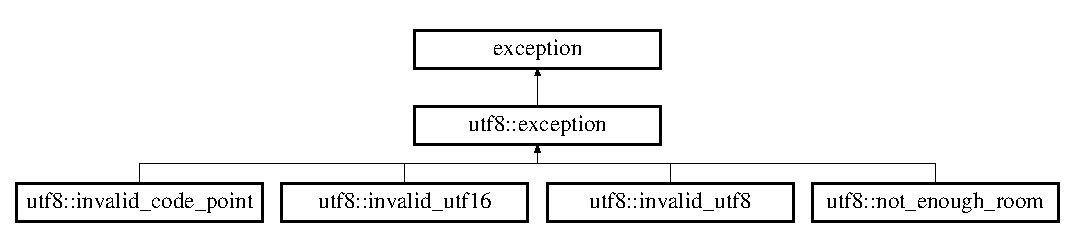
\includegraphics[height=2.745098cm]{classutf8_1_1exception}
\end{center}
\end{figure}


The documentation for this class was generated from the following file\+:\begin{DoxyCompactItemize}
\item 
C\+:/cygwin/home/\+Engineer/\+Development/time-\/clock-\/front/\+Q\+B\+Wrapper/\+U\+T\+F-\/8/utf8/\hyperlink{checked_8h}{checked.\+h}\end{DoxyCompactItemize}

\hypertarget{classutf8_1_1invalid__code__point}{}\section{utf8\+:\+:invalid\+\_\+code\+\_\+point Class Reference}
\label{classutf8_1_1invalid__code__point}\index{utf8\+::invalid\+\_\+code\+\_\+point@{utf8\+::invalid\+\_\+code\+\_\+point}}


{\ttfamily \#include $<$checked.\+h$>$}

Inheritance diagram for utf8\+:\+:invalid\+\_\+code\+\_\+point\+:\begin{figure}[H]
\begin{center}
\leavevmode
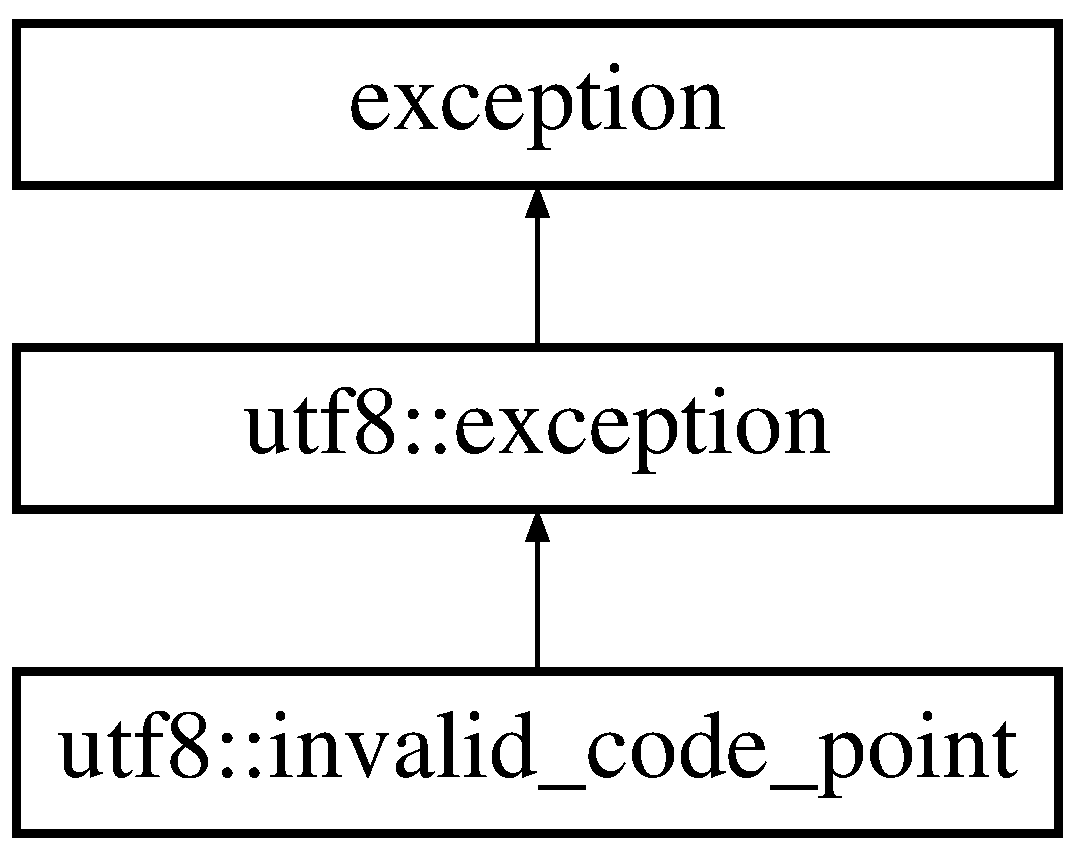
\includegraphics[height=3.000000cm]{classutf8_1_1invalid__code__point}
\end{center}
\end{figure}
\subsection*{Public Member Functions}
\begin{DoxyCompactItemize}
\item 
\hyperlink{classutf8_1_1invalid__code__point_a46f27dd1c5b286936ec58baca3ca6220}{invalid\+\_\+code\+\_\+point} (\hyperlink{namespaceutf8_a846259d2f173d524282583fc9d825b00}{uint32\+\_\+t} cp)
\item 
virtual const char $\ast$ \hyperlink{classutf8_1_1invalid__code__point_ada45ed42142e57e7e1693bbac6985dce}{what} () const   throw ()
\item 
\hyperlink{namespaceutf8_a846259d2f173d524282583fc9d825b00}{uint32\+\_\+t} \hyperlink{classutf8_1_1invalid__code__point_a07539c0ef6aa826178f56b9d53d475af}{code\+\_\+point} () const 
\end{DoxyCompactItemize}


\subsection{Constructor \& Destructor Documentation}
\hypertarget{classutf8_1_1invalid__code__point_a46f27dd1c5b286936ec58baca3ca6220}{}\index{utf8\+::invalid\+\_\+code\+\_\+point@{utf8\+::invalid\+\_\+code\+\_\+point}!invalid\+\_\+code\+\_\+point@{invalid\+\_\+code\+\_\+point}}
\index{invalid\+\_\+code\+\_\+point@{invalid\+\_\+code\+\_\+point}!utf8\+::invalid\+\_\+code\+\_\+point@{utf8\+::invalid\+\_\+code\+\_\+point}}
\subsubsection[{invalid\+\_\+code\+\_\+point}]{\setlength{\rightskip}{0pt plus 5cm}utf8\+::invalid\+\_\+code\+\_\+point\+::invalid\+\_\+code\+\_\+point (
\begin{DoxyParamCaption}
\item[{{\bf uint32\+\_\+t}}]{cp}
\end{DoxyParamCaption}
)\hspace{0.3cm}{\ttfamily [inline]}}\label{classutf8_1_1invalid__code__point_a46f27dd1c5b286936ec58baca3ca6220}


\subsection{Member Function Documentation}
\hypertarget{classutf8_1_1invalid__code__point_a07539c0ef6aa826178f56b9d53d475af}{}\index{utf8\+::invalid\+\_\+code\+\_\+point@{utf8\+::invalid\+\_\+code\+\_\+point}!code\+\_\+point@{code\+\_\+point}}
\index{code\+\_\+point@{code\+\_\+point}!utf8\+::invalid\+\_\+code\+\_\+point@{utf8\+::invalid\+\_\+code\+\_\+point}}
\subsubsection[{code\+\_\+point}]{\setlength{\rightskip}{0pt plus 5cm}{\bf uint32\+\_\+t} utf8\+::invalid\+\_\+code\+\_\+point\+::code\+\_\+point (
\begin{DoxyParamCaption}
{}
\end{DoxyParamCaption}
) const\hspace{0.3cm}{\ttfamily [inline]}}\label{classutf8_1_1invalid__code__point_a07539c0ef6aa826178f56b9d53d475af}
\hypertarget{classutf8_1_1invalid__code__point_ada45ed42142e57e7e1693bbac6985dce}{}\index{utf8\+::invalid\+\_\+code\+\_\+point@{utf8\+::invalid\+\_\+code\+\_\+point}!what@{what}}
\index{what@{what}!utf8\+::invalid\+\_\+code\+\_\+point@{utf8\+::invalid\+\_\+code\+\_\+point}}
\subsubsection[{what}]{\setlength{\rightskip}{0pt plus 5cm}virtual const char$\ast$ utf8\+::invalid\+\_\+code\+\_\+point\+::what (
\begin{DoxyParamCaption}
{}
\end{DoxyParamCaption}
) const throw  ) \hspace{0.3cm}{\ttfamily [inline]}, {\ttfamily [virtual]}}\label{classutf8_1_1invalid__code__point_ada45ed42142e57e7e1693bbac6985dce}


The documentation for this class was generated from the following file\+:\begin{DoxyCompactItemize}
\item 
C\+:/cygwin/home/\+Engineer/\+Development/time-\/clock-\/front/\+Q\+B\+Wrapper/\+U\+T\+F-\/8/utf8/\hyperlink{checked_8h}{checked.\+h}\end{DoxyCompactItemize}

\hypertarget{classutf8_1_1invalid__utf16}{}\section{utf8\+:\+:invalid\+\_\+utf16 Class Reference}
\label{classutf8_1_1invalid__utf16}\index{utf8\+::invalid\+\_\+utf16@{utf8\+::invalid\+\_\+utf16}}


{\ttfamily \#include $<$checked.\+h$>$}

Inheritance diagram for utf8\+:\+:invalid\+\_\+utf16\+:\begin{figure}[H]
\begin{center}
\leavevmode
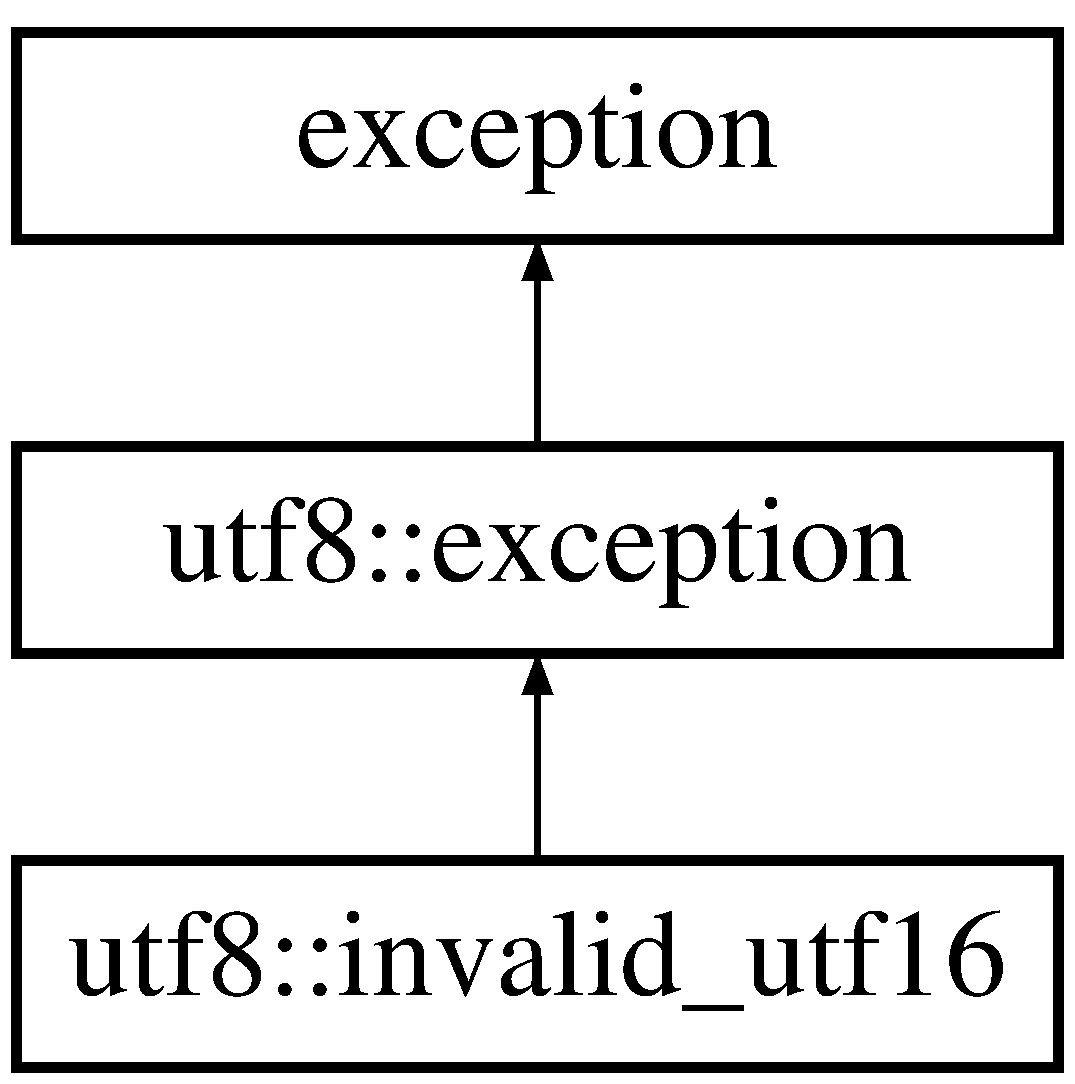
\includegraphics[height=3.000000cm]{classutf8_1_1invalid__utf16}
\end{center}
\end{figure}
\subsection*{Public Member Functions}
\begin{DoxyCompactItemize}
\item 
\hyperlink{classutf8_1_1invalid__utf16_a83f8d198986495279499cfba0f44f9e5}{invalid\+\_\+utf16} (\hyperlink{namespaceutf8_ac23066b92c5a1d9d9ef177201f750936}{uint16\+\_\+t} u)
\item 
virtual const char $\ast$ \hyperlink{classutf8_1_1invalid__utf16_a70fd20978a50030a2f364e0da08346f6}{what} () const   throw ()
\item 
\hyperlink{namespaceutf8_ac23066b92c5a1d9d9ef177201f750936}{uint16\+\_\+t} \hyperlink{classutf8_1_1invalid__utf16_a514a11e2df0c73edd4afcccc89317c4b}{utf16\+\_\+word} () const 
\end{DoxyCompactItemize}


\subsection{Constructor \& Destructor Documentation}
\hypertarget{classutf8_1_1invalid__utf16_a83f8d198986495279499cfba0f44f9e5}{}\index{utf8\+::invalid\+\_\+utf16@{utf8\+::invalid\+\_\+utf16}!invalid\+\_\+utf16@{invalid\+\_\+utf16}}
\index{invalid\+\_\+utf16@{invalid\+\_\+utf16}!utf8\+::invalid\+\_\+utf16@{utf8\+::invalid\+\_\+utf16}}
\subsubsection[{invalid\+\_\+utf16}]{\setlength{\rightskip}{0pt plus 5cm}utf8\+::invalid\+\_\+utf16\+::invalid\+\_\+utf16 (
\begin{DoxyParamCaption}
\item[{{\bf uint16\+\_\+t}}]{u}
\end{DoxyParamCaption}
)\hspace{0.3cm}{\ttfamily [inline]}}\label{classutf8_1_1invalid__utf16_a83f8d198986495279499cfba0f44f9e5}


\subsection{Member Function Documentation}
\hypertarget{classutf8_1_1invalid__utf16_a514a11e2df0c73edd4afcccc89317c4b}{}\index{utf8\+::invalid\+\_\+utf16@{utf8\+::invalid\+\_\+utf16}!utf16\+\_\+word@{utf16\+\_\+word}}
\index{utf16\+\_\+word@{utf16\+\_\+word}!utf8\+::invalid\+\_\+utf16@{utf8\+::invalid\+\_\+utf16}}
\subsubsection[{utf16\+\_\+word}]{\setlength{\rightskip}{0pt plus 5cm}{\bf uint16\+\_\+t} utf8\+::invalid\+\_\+utf16\+::utf16\+\_\+word (
\begin{DoxyParamCaption}
{}
\end{DoxyParamCaption}
) const\hspace{0.3cm}{\ttfamily [inline]}}\label{classutf8_1_1invalid__utf16_a514a11e2df0c73edd4afcccc89317c4b}
\hypertarget{classutf8_1_1invalid__utf16_a70fd20978a50030a2f364e0da08346f6}{}\index{utf8\+::invalid\+\_\+utf16@{utf8\+::invalid\+\_\+utf16}!what@{what}}
\index{what@{what}!utf8\+::invalid\+\_\+utf16@{utf8\+::invalid\+\_\+utf16}}
\subsubsection[{what}]{\setlength{\rightskip}{0pt plus 5cm}virtual const char$\ast$ utf8\+::invalid\+\_\+utf16\+::what (
\begin{DoxyParamCaption}
{}
\end{DoxyParamCaption}
) const throw  ) \hspace{0.3cm}{\ttfamily [inline]}, {\ttfamily [virtual]}}\label{classutf8_1_1invalid__utf16_a70fd20978a50030a2f364e0da08346f6}


The documentation for this class was generated from the following file\+:\begin{DoxyCompactItemize}
\item 
C\+:/cygwin/home/\+Engineer/\+Development/time-\/clock-\/front/\+Q\+B\+Wrapper/\+U\+T\+F-\/8/utf8/\hyperlink{checked_8h}{checked.\+h}\end{DoxyCompactItemize}

\hypertarget{classutf8_1_1invalid__utf8}{}\section{utf8\+:\+:invalid\+\_\+utf8 Class Reference}
\label{classutf8_1_1invalid__utf8}\index{utf8\+::invalid\+\_\+utf8@{utf8\+::invalid\+\_\+utf8}}


{\ttfamily \#include $<$checked.\+h$>$}

Inheritance diagram for utf8\+:\+:invalid\+\_\+utf8\+:\begin{figure}[H]
\begin{center}
\leavevmode
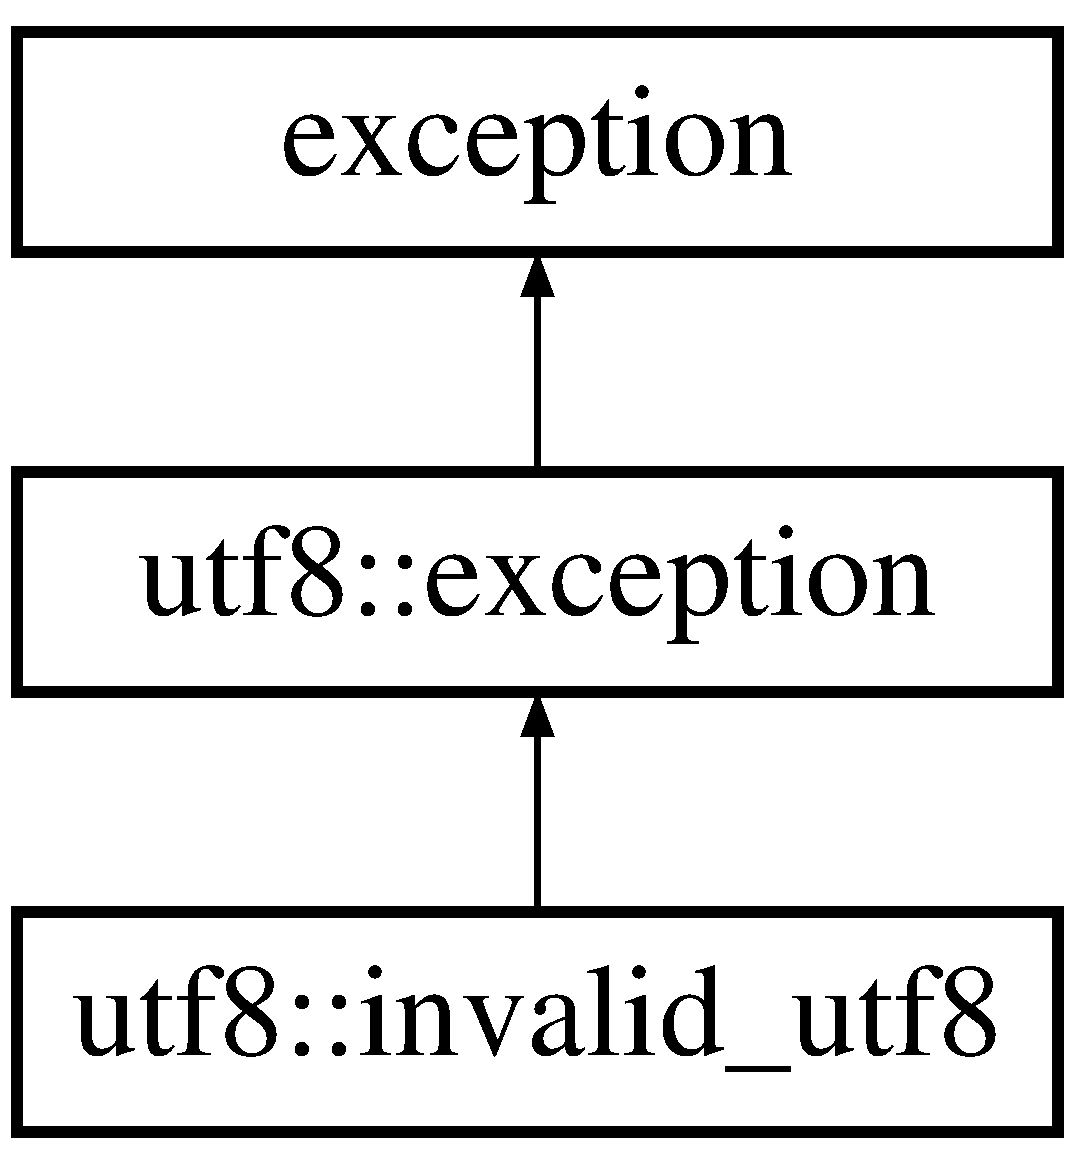
\includegraphics[height=3.000000cm]{classutf8_1_1invalid__utf8}
\end{center}
\end{figure}
\subsection*{Public Member Functions}
\begin{DoxyCompactItemize}
\item 
\hyperlink{classutf8_1_1invalid__utf8_a161e63ef9ceb25f5e916d7b580d001a0}{invalid\+\_\+utf8} (\hyperlink{namespaceutf8_abe793b552fabe390d134b97ab81d2c7f}{uint8\+\_\+t} u)
\item 
virtual const char $\ast$ \hyperlink{classutf8_1_1invalid__utf8_ae142c084e0a6ded9c186d09879d97036}{what} () const   throw ()
\item 
\hyperlink{namespaceutf8_abe793b552fabe390d134b97ab81d2c7f}{uint8\+\_\+t} \hyperlink{classutf8_1_1invalid__utf8_ab5f53ce0be75c4eeee078f471ce40a7b}{utf8\+\_\+octet} () const 
\end{DoxyCompactItemize}


\subsection{Constructor \& Destructor Documentation}
\hypertarget{classutf8_1_1invalid__utf8_a161e63ef9ceb25f5e916d7b580d001a0}{}\index{utf8\+::invalid\+\_\+utf8@{utf8\+::invalid\+\_\+utf8}!invalid\+\_\+utf8@{invalid\+\_\+utf8}}
\index{invalid\+\_\+utf8@{invalid\+\_\+utf8}!utf8\+::invalid\+\_\+utf8@{utf8\+::invalid\+\_\+utf8}}
\subsubsection[{invalid\+\_\+utf8}]{\setlength{\rightskip}{0pt plus 5cm}utf8\+::invalid\+\_\+utf8\+::invalid\+\_\+utf8 (
\begin{DoxyParamCaption}
\item[{{\bf uint8\+\_\+t}}]{u}
\end{DoxyParamCaption}
)\hspace{0.3cm}{\ttfamily [inline]}}\label{classutf8_1_1invalid__utf8_a161e63ef9ceb25f5e916d7b580d001a0}


\subsection{Member Function Documentation}
\hypertarget{classutf8_1_1invalid__utf8_ab5f53ce0be75c4eeee078f471ce40a7b}{}\index{utf8\+::invalid\+\_\+utf8@{utf8\+::invalid\+\_\+utf8}!utf8\+\_\+octet@{utf8\+\_\+octet}}
\index{utf8\+\_\+octet@{utf8\+\_\+octet}!utf8\+::invalid\+\_\+utf8@{utf8\+::invalid\+\_\+utf8}}
\subsubsection[{utf8\+\_\+octet}]{\setlength{\rightskip}{0pt plus 5cm}{\bf uint8\+\_\+t} utf8\+::invalid\+\_\+utf8\+::utf8\+\_\+octet (
\begin{DoxyParamCaption}
{}
\end{DoxyParamCaption}
) const\hspace{0.3cm}{\ttfamily [inline]}}\label{classutf8_1_1invalid__utf8_ab5f53ce0be75c4eeee078f471ce40a7b}
\hypertarget{classutf8_1_1invalid__utf8_ae142c084e0a6ded9c186d09879d97036}{}\index{utf8\+::invalid\+\_\+utf8@{utf8\+::invalid\+\_\+utf8}!what@{what}}
\index{what@{what}!utf8\+::invalid\+\_\+utf8@{utf8\+::invalid\+\_\+utf8}}
\subsubsection[{what}]{\setlength{\rightskip}{0pt plus 5cm}virtual const char$\ast$ utf8\+::invalid\+\_\+utf8\+::what (
\begin{DoxyParamCaption}
{}
\end{DoxyParamCaption}
) const throw  ) \hspace{0.3cm}{\ttfamily [inline]}, {\ttfamily [virtual]}}\label{classutf8_1_1invalid__utf8_ae142c084e0a6ded9c186d09879d97036}


The documentation for this class was generated from the following file\+:\begin{DoxyCompactItemize}
\item 
C\+:/cygwin/home/\+Engineer/\+Development/time-\/clock-\/front/\+Q\+B\+Wrapper/\+U\+T\+F-\/8/utf8/\hyperlink{checked_8h}{checked.\+h}\end{DoxyCompactItemize}

\hypertarget{classutf8_1_1unchecked_1_1iterator}{}\section{utf8\+:\+:unchecked\+:\+:iterator$<$ octet\+\_\+iterator $>$ Class Template Reference}
\label{classutf8_1_1unchecked_1_1iterator}\index{utf8\+::unchecked\+::iterator$<$ octet\+\_\+iterator $>$@{utf8\+::unchecked\+::iterator$<$ octet\+\_\+iterator $>$}}


{\ttfamily \#include $<$unchecked.\+h$>$}

Inheritance diagram for utf8\+:\+:unchecked\+:\+:iterator$<$ octet\+\_\+iterator $>$\+:\begin{figure}[H]
\begin{center}
\leavevmode
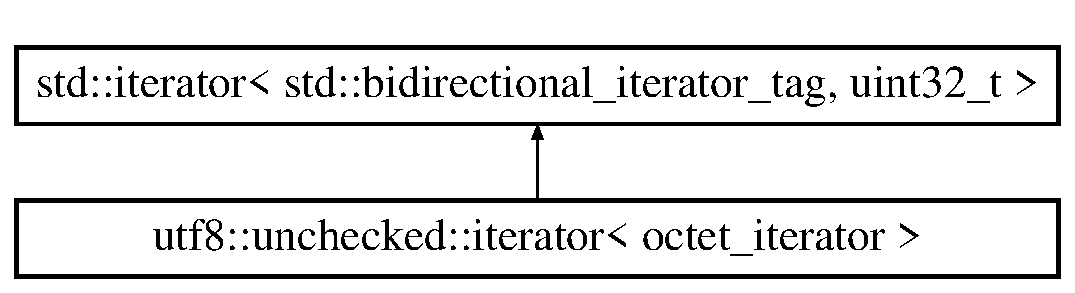
\includegraphics[height=2.000000cm]{classutf8_1_1unchecked_1_1iterator}
\end{center}
\end{figure}
\subsection*{Public Member Functions}
\begin{DoxyCompactItemize}
\item 
\hyperlink{classutf8_1_1unchecked_1_1iterator_a6564ecea96a82b87daca60a153ee1a6f}{iterator} ()
\item 
\hyperlink{classutf8_1_1unchecked_1_1iterator_a0f93d81989f2eb1038c0550431b9653b}{iterator} (const octet\+\_\+iterator \&octet\+\_\+it)
\item 
octet\+\_\+iterator \hyperlink{classutf8_1_1unchecked_1_1iterator_a9aca104f445e27a31fd755dcad2a5b60}{base} () const 
\item 
\hyperlink{namespaceutf8_a846259d2f173d524282583fc9d825b00}{uint32\+\_\+t} \hyperlink{classutf8_1_1unchecked_1_1iterator_a06b0df26a8570080c756f8d9a4cfdf76}{operator$\ast$} () const 
\item 
bool \hyperlink{classutf8_1_1unchecked_1_1iterator_aabb0ce8d23aa99bdddc70b9f41ee9d9a}{operator==} (const \hyperlink{classutf8_1_1unchecked_1_1iterator}{iterator} \&rhs) const 
\item 
bool \hyperlink{classutf8_1_1unchecked_1_1iterator_afd83ba10f6b423665e6b376759b21026}{operator!=} (const \hyperlink{classutf8_1_1unchecked_1_1iterator}{iterator} \&rhs) const 
\item 
\hyperlink{classutf8_1_1unchecked_1_1iterator}{iterator} \& \hyperlink{classutf8_1_1unchecked_1_1iterator_a0450ee39cf7eeed074d229fb9b6b22bc}{operator++} ()
\item 
\hyperlink{classutf8_1_1unchecked_1_1iterator}{iterator} \hyperlink{classutf8_1_1unchecked_1_1iterator_ae1cadaddd5c1db5518def5af491a1ff1}{operator++} (int)
\item 
\hyperlink{classutf8_1_1unchecked_1_1iterator}{iterator} \& \hyperlink{classutf8_1_1unchecked_1_1iterator_a8b50b3a0d7b2c2506e135db73a636c7b}{operator-\/-\/} ()
\item 
\hyperlink{classutf8_1_1unchecked_1_1iterator}{iterator} \hyperlink{classutf8_1_1unchecked_1_1iterator_a85597f5ae4bd175edb6dc2fc9ceb2f34}{operator-\/-\/} (int)
\end{DoxyCompactItemize}


\subsection{Constructor \& Destructor Documentation}
\hypertarget{classutf8_1_1unchecked_1_1iterator_a6564ecea96a82b87daca60a153ee1a6f}{}\index{utf8\+::unchecked\+::iterator@{utf8\+::unchecked\+::iterator}!iterator@{iterator}}
\index{iterator@{iterator}!utf8\+::unchecked\+::iterator@{utf8\+::unchecked\+::iterator}}
\subsubsection[{iterator}]{\setlength{\rightskip}{0pt plus 5cm}template$<$typename octet\+\_\+iterator $>$ {\bf utf8\+::unchecked\+::iterator}$<$ octet\+\_\+iterator $>$\+::{\bf iterator} (
\begin{DoxyParamCaption}
{}
\end{DoxyParamCaption}
)\hspace{0.3cm}{\ttfamily [inline]}}\label{classutf8_1_1unchecked_1_1iterator_a6564ecea96a82b87daca60a153ee1a6f}
\hypertarget{classutf8_1_1unchecked_1_1iterator_a0f93d81989f2eb1038c0550431b9653b}{}\index{utf8\+::unchecked\+::iterator@{utf8\+::unchecked\+::iterator}!iterator@{iterator}}
\index{iterator@{iterator}!utf8\+::unchecked\+::iterator@{utf8\+::unchecked\+::iterator}}
\subsubsection[{iterator}]{\setlength{\rightskip}{0pt plus 5cm}template$<$typename octet\+\_\+iterator $>$ {\bf utf8\+::unchecked\+::iterator}$<$ octet\+\_\+iterator $>$\+::{\bf iterator} (
\begin{DoxyParamCaption}
\item[{const octet\+\_\+iterator$<$ octet\+\_\+iterator $>$ \&}]{octet\+\_\+it}
\end{DoxyParamCaption}
)\hspace{0.3cm}{\ttfamily [inline]}, {\ttfamily [explicit]}}\label{classutf8_1_1unchecked_1_1iterator_a0f93d81989f2eb1038c0550431b9653b}


\subsection{Member Function Documentation}
\hypertarget{classutf8_1_1unchecked_1_1iterator_a9aca104f445e27a31fd755dcad2a5b60}{}\index{utf8\+::unchecked\+::iterator@{utf8\+::unchecked\+::iterator}!base@{base}}
\index{base@{base}!utf8\+::unchecked\+::iterator@{utf8\+::unchecked\+::iterator}}
\subsubsection[{base}]{\setlength{\rightskip}{0pt plus 5cm}template$<$typename octet\+\_\+iterator $>$ octet\+\_\+iterator {\bf utf8\+::unchecked\+::iterator}$<$ octet\+\_\+iterator $>$\+::base (
\begin{DoxyParamCaption}
{}
\end{DoxyParamCaption}
) const\hspace{0.3cm}{\ttfamily [inline]}}\label{classutf8_1_1unchecked_1_1iterator_a9aca104f445e27a31fd755dcad2a5b60}
\hypertarget{classutf8_1_1unchecked_1_1iterator_afd83ba10f6b423665e6b376759b21026}{}\index{utf8\+::unchecked\+::iterator@{utf8\+::unchecked\+::iterator}!operator"!=@{operator"!=}}
\index{operator"!=@{operator"!=}!utf8\+::unchecked\+::iterator@{utf8\+::unchecked\+::iterator}}
\subsubsection[{operator"!=}]{\setlength{\rightskip}{0pt plus 5cm}template$<$typename octet\+\_\+iterator $>$ bool {\bf utf8\+::unchecked\+::iterator}$<$ octet\+\_\+iterator $>$\+::operator!= (
\begin{DoxyParamCaption}
\item[{const {\bf iterator}$<$ octet\+\_\+iterator $>$ \&}]{rhs}
\end{DoxyParamCaption}
) const\hspace{0.3cm}{\ttfamily [inline]}}\label{classutf8_1_1unchecked_1_1iterator_afd83ba10f6b423665e6b376759b21026}
\hypertarget{classutf8_1_1unchecked_1_1iterator_a06b0df26a8570080c756f8d9a4cfdf76}{}\index{utf8\+::unchecked\+::iterator@{utf8\+::unchecked\+::iterator}!operator$\ast$@{operator$\ast$}}
\index{operator$\ast$@{operator$\ast$}!utf8\+::unchecked\+::iterator@{utf8\+::unchecked\+::iterator}}
\subsubsection[{operator$\ast$}]{\setlength{\rightskip}{0pt plus 5cm}template$<$typename octet\+\_\+iterator $>$ {\bf uint32\+\_\+t} {\bf utf8\+::unchecked\+::iterator}$<$ octet\+\_\+iterator $>$\+::operator$\ast$ (
\begin{DoxyParamCaption}
{}
\end{DoxyParamCaption}
) const\hspace{0.3cm}{\ttfamily [inline]}}\label{classutf8_1_1unchecked_1_1iterator_a06b0df26a8570080c756f8d9a4cfdf76}
\hypertarget{classutf8_1_1unchecked_1_1iterator_a0450ee39cf7eeed074d229fb9b6b22bc}{}\index{utf8\+::unchecked\+::iterator@{utf8\+::unchecked\+::iterator}!operator++@{operator++}}
\index{operator++@{operator++}!utf8\+::unchecked\+::iterator@{utf8\+::unchecked\+::iterator}}
\subsubsection[{operator++}]{\setlength{\rightskip}{0pt plus 5cm}template$<$typename octet\+\_\+iterator $>$ {\bf iterator}\& {\bf utf8\+::unchecked\+::iterator}$<$ octet\+\_\+iterator $>$\+::operator++ (
\begin{DoxyParamCaption}
{}
\end{DoxyParamCaption}
)\hspace{0.3cm}{\ttfamily [inline]}}\label{classutf8_1_1unchecked_1_1iterator_a0450ee39cf7eeed074d229fb9b6b22bc}
\hypertarget{classutf8_1_1unchecked_1_1iterator_ae1cadaddd5c1db5518def5af491a1ff1}{}\index{utf8\+::unchecked\+::iterator@{utf8\+::unchecked\+::iterator}!operator++@{operator++}}
\index{operator++@{operator++}!utf8\+::unchecked\+::iterator@{utf8\+::unchecked\+::iterator}}
\subsubsection[{operator++}]{\setlength{\rightskip}{0pt plus 5cm}template$<$typename octet\+\_\+iterator $>$ {\bf iterator} {\bf utf8\+::unchecked\+::iterator}$<$ octet\+\_\+iterator $>$\+::operator++ (
\begin{DoxyParamCaption}
\item[{int}]{}
\end{DoxyParamCaption}
)\hspace{0.3cm}{\ttfamily [inline]}}\label{classutf8_1_1unchecked_1_1iterator_ae1cadaddd5c1db5518def5af491a1ff1}
\hypertarget{classutf8_1_1unchecked_1_1iterator_a8b50b3a0d7b2c2506e135db73a636c7b}{}\index{utf8\+::unchecked\+::iterator@{utf8\+::unchecked\+::iterator}!operator-\/-\/@{operator-\/-\/}}
\index{operator-\/-\/@{operator-\/-\/}!utf8\+::unchecked\+::iterator@{utf8\+::unchecked\+::iterator}}
\subsubsection[{operator-\/-\/}]{\setlength{\rightskip}{0pt plus 5cm}template$<$typename octet\+\_\+iterator $>$ {\bf iterator}\& {\bf utf8\+::unchecked\+::iterator}$<$ octet\+\_\+iterator $>$\+::operator-\/-\/ (
\begin{DoxyParamCaption}
{}
\end{DoxyParamCaption}
)\hspace{0.3cm}{\ttfamily [inline]}}\label{classutf8_1_1unchecked_1_1iterator_a8b50b3a0d7b2c2506e135db73a636c7b}
\hypertarget{classutf8_1_1unchecked_1_1iterator_a85597f5ae4bd175edb6dc2fc9ceb2f34}{}\index{utf8\+::unchecked\+::iterator@{utf8\+::unchecked\+::iterator}!operator-\/-\/@{operator-\/-\/}}
\index{operator-\/-\/@{operator-\/-\/}!utf8\+::unchecked\+::iterator@{utf8\+::unchecked\+::iterator}}
\subsubsection[{operator-\/-\/}]{\setlength{\rightskip}{0pt plus 5cm}template$<$typename octet\+\_\+iterator $>$ {\bf iterator} {\bf utf8\+::unchecked\+::iterator}$<$ octet\+\_\+iterator $>$\+::operator-\/-\/ (
\begin{DoxyParamCaption}
\item[{int}]{}
\end{DoxyParamCaption}
)\hspace{0.3cm}{\ttfamily [inline]}}\label{classutf8_1_1unchecked_1_1iterator_a85597f5ae4bd175edb6dc2fc9ceb2f34}
\hypertarget{classutf8_1_1unchecked_1_1iterator_aabb0ce8d23aa99bdddc70b9f41ee9d9a}{}\index{utf8\+::unchecked\+::iterator@{utf8\+::unchecked\+::iterator}!operator==@{operator==}}
\index{operator==@{operator==}!utf8\+::unchecked\+::iterator@{utf8\+::unchecked\+::iterator}}
\subsubsection[{operator==}]{\setlength{\rightskip}{0pt plus 5cm}template$<$typename octet\+\_\+iterator $>$ bool {\bf utf8\+::unchecked\+::iterator}$<$ octet\+\_\+iterator $>$\+::operator== (
\begin{DoxyParamCaption}
\item[{const {\bf iterator}$<$ octet\+\_\+iterator $>$ \&}]{rhs}
\end{DoxyParamCaption}
) const\hspace{0.3cm}{\ttfamily [inline]}}\label{classutf8_1_1unchecked_1_1iterator_aabb0ce8d23aa99bdddc70b9f41ee9d9a}


The documentation for this class was generated from the following file\+:\begin{DoxyCompactItemize}
\item 
C\+:/cygwin/home/\+Engineer/\+Development/time-\/clock-\/front/\+Q\+B\+Wrapper/\+U\+T\+F-\/8/utf8/\hyperlink{unchecked_8h}{unchecked.\+h}\end{DoxyCompactItemize}

\hypertarget{classutf8_1_1iterator}{}\section{utf8\+:\+:iterator$<$ octet\+\_\+iterator $>$ Class Template Reference}
\label{classutf8_1_1iterator}\index{utf8\+::iterator$<$ octet\+\_\+iterator $>$@{utf8\+::iterator$<$ octet\+\_\+iterator $>$}}


{\ttfamily \#include $<$checked.\+h$>$}

Inheritance diagram for utf8\+:\+:iterator$<$ octet\+\_\+iterator $>$\+:\begin{figure}[H]
\begin{center}
\leavevmode
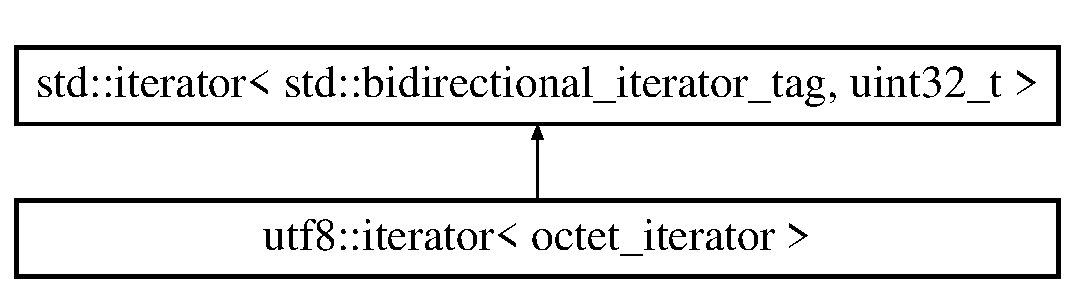
\includegraphics[height=2.000000cm]{classutf8_1_1iterator}
\end{center}
\end{figure}
\subsection*{Public Member Functions}
\begin{DoxyCompactItemize}
\item 
\hyperlink{classutf8_1_1iterator_a507000943ac3fdfe59331dac3c35c6bd}{iterator} ()
\item 
\hyperlink{classutf8_1_1iterator_a85a9cb70e9e77d2d04eba61612b5ef13}{iterator} (const octet\+\_\+iterator \&octet\+\_\+it, const octet\+\_\+iterator \&range\+\_\+start, const octet\+\_\+iterator \&range\+\_\+end)
\item 
octet\+\_\+iterator \hyperlink{classutf8_1_1iterator_aec700ec9689fe88ebe9a7fe1feca8d2d}{base} () const 
\item 
\hyperlink{namespaceutf8_a846259d2f173d524282583fc9d825b00}{uint32\+\_\+t} \hyperlink{classutf8_1_1iterator_abbe7cf79cc5b78a375d80b0dba39fa0c}{operator$\ast$} () const 
\item 
bool \hyperlink{classutf8_1_1iterator_a0527930d64be7835f881bf649a317cfb}{operator==} (const \hyperlink{classutf8_1_1iterator}{iterator} \&rhs) const 
\item 
bool \hyperlink{classutf8_1_1iterator_a6be99d96bf62e7e0d9f1bdc1841efb3c}{operator!=} (const \hyperlink{classutf8_1_1iterator}{iterator} \&rhs) const 
\item 
\hyperlink{classutf8_1_1iterator}{iterator} \& \hyperlink{classutf8_1_1iterator_a93e9ac16a560fab545a05efb6b0a3add}{operator++} ()
\item 
\hyperlink{classutf8_1_1iterator}{iterator} \hyperlink{classutf8_1_1iterator_aa21c39e32e3bf53c08d8ee5cde280671}{operator++} (int)
\item 
\hyperlink{classutf8_1_1iterator}{iterator} \& \hyperlink{classutf8_1_1iterator_a7781099a85323b5a3ff4dc1015ca5af0}{operator-\/-\/} ()
\item 
\hyperlink{classutf8_1_1iterator}{iterator} \hyperlink{classutf8_1_1iterator_afc228985ba672a6b6966ea0a705a4755}{operator-\/-\/} (int)
\end{DoxyCompactItemize}


\subsection{Constructor \& Destructor Documentation}
\hypertarget{classutf8_1_1iterator_a507000943ac3fdfe59331dac3c35c6bd}{}\index{utf8\+::iterator@{utf8\+::iterator}!iterator@{iterator}}
\index{iterator@{iterator}!utf8\+::iterator@{utf8\+::iterator}}
\subsubsection[{iterator}]{\setlength{\rightskip}{0pt plus 5cm}template$<$typename octet\+\_\+iterator $>$ {\bf utf8\+::iterator}$<$ octet\+\_\+iterator $>$\+::{\bf iterator} (
\begin{DoxyParamCaption}
{}
\end{DoxyParamCaption}
)\hspace{0.3cm}{\ttfamily [inline]}}\label{classutf8_1_1iterator_a507000943ac3fdfe59331dac3c35c6bd}
\hypertarget{classutf8_1_1iterator_a85a9cb70e9e77d2d04eba61612b5ef13}{}\index{utf8\+::iterator@{utf8\+::iterator}!iterator@{iterator}}
\index{iterator@{iterator}!utf8\+::iterator@{utf8\+::iterator}}
\subsubsection[{iterator}]{\setlength{\rightskip}{0pt plus 5cm}template$<$typename octet\+\_\+iterator $>$ {\bf utf8\+::iterator}$<$ octet\+\_\+iterator $>$\+::{\bf iterator} (
\begin{DoxyParamCaption}
\item[{const octet\+\_\+iterator$<$ octet\+\_\+iterator $>$ \&}]{octet\+\_\+it, }
\item[{const octet\+\_\+iterator$<$ octet\+\_\+iterator $>$ \&}]{range\+\_\+start, }
\item[{const octet\+\_\+iterator$<$ octet\+\_\+iterator $>$ \&}]{range\+\_\+end}
\end{DoxyParamCaption}
)\hspace{0.3cm}{\ttfamily [inline]}, {\ttfamily [explicit]}}\label{classutf8_1_1iterator_a85a9cb70e9e77d2d04eba61612b5ef13}


\subsection{Member Function Documentation}
\hypertarget{classutf8_1_1iterator_aec700ec9689fe88ebe9a7fe1feca8d2d}{}\index{utf8\+::iterator@{utf8\+::iterator}!base@{base}}
\index{base@{base}!utf8\+::iterator@{utf8\+::iterator}}
\subsubsection[{base}]{\setlength{\rightskip}{0pt plus 5cm}template$<$typename octet\+\_\+iterator $>$ octet\+\_\+iterator {\bf utf8\+::iterator}$<$ octet\+\_\+iterator $>$\+::base (
\begin{DoxyParamCaption}
{}
\end{DoxyParamCaption}
) const\hspace{0.3cm}{\ttfamily [inline]}}\label{classutf8_1_1iterator_aec700ec9689fe88ebe9a7fe1feca8d2d}
\hypertarget{classutf8_1_1iterator_a6be99d96bf62e7e0d9f1bdc1841efb3c}{}\index{utf8\+::iterator@{utf8\+::iterator}!operator"!=@{operator"!=}}
\index{operator"!=@{operator"!=}!utf8\+::iterator@{utf8\+::iterator}}
\subsubsection[{operator"!=}]{\setlength{\rightskip}{0pt plus 5cm}template$<$typename octet\+\_\+iterator $>$ bool {\bf utf8\+::iterator}$<$ octet\+\_\+iterator $>$\+::operator!= (
\begin{DoxyParamCaption}
\item[{const {\bf iterator}$<$ octet\+\_\+iterator $>$ \&}]{rhs}
\end{DoxyParamCaption}
) const\hspace{0.3cm}{\ttfamily [inline]}}\label{classutf8_1_1iterator_a6be99d96bf62e7e0d9f1bdc1841efb3c}
\hypertarget{classutf8_1_1iterator_abbe7cf79cc5b78a375d80b0dba39fa0c}{}\index{utf8\+::iterator@{utf8\+::iterator}!operator$\ast$@{operator$\ast$}}
\index{operator$\ast$@{operator$\ast$}!utf8\+::iterator@{utf8\+::iterator}}
\subsubsection[{operator$\ast$}]{\setlength{\rightskip}{0pt plus 5cm}template$<$typename octet\+\_\+iterator $>$ {\bf uint32\+\_\+t} {\bf utf8\+::iterator}$<$ octet\+\_\+iterator $>$\+::operator$\ast$ (
\begin{DoxyParamCaption}
{}
\end{DoxyParamCaption}
) const\hspace{0.3cm}{\ttfamily [inline]}}\label{classutf8_1_1iterator_abbe7cf79cc5b78a375d80b0dba39fa0c}
\hypertarget{classutf8_1_1iterator_a93e9ac16a560fab545a05efb6b0a3add}{}\index{utf8\+::iterator@{utf8\+::iterator}!operator++@{operator++}}
\index{operator++@{operator++}!utf8\+::iterator@{utf8\+::iterator}}
\subsubsection[{operator++}]{\setlength{\rightskip}{0pt plus 5cm}template$<$typename octet\+\_\+iterator $>$ {\bf iterator}\& {\bf utf8\+::iterator}$<$ octet\+\_\+iterator $>$\+::operator++ (
\begin{DoxyParamCaption}
{}
\end{DoxyParamCaption}
)\hspace{0.3cm}{\ttfamily [inline]}}\label{classutf8_1_1iterator_a93e9ac16a560fab545a05efb6b0a3add}
\hypertarget{classutf8_1_1iterator_aa21c39e32e3bf53c08d8ee5cde280671}{}\index{utf8\+::iterator@{utf8\+::iterator}!operator++@{operator++}}
\index{operator++@{operator++}!utf8\+::iterator@{utf8\+::iterator}}
\subsubsection[{operator++}]{\setlength{\rightskip}{0pt plus 5cm}template$<$typename octet\+\_\+iterator $>$ {\bf iterator} {\bf utf8\+::iterator}$<$ octet\+\_\+iterator $>$\+::operator++ (
\begin{DoxyParamCaption}
\item[{int}]{}
\end{DoxyParamCaption}
)\hspace{0.3cm}{\ttfamily [inline]}}\label{classutf8_1_1iterator_aa21c39e32e3bf53c08d8ee5cde280671}
\hypertarget{classutf8_1_1iterator_a7781099a85323b5a3ff4dc1015ca5af0}{}\index{utf8\+::iterator@{utf8\+::iterator}!operator-\/-\/@{operator-\/-\/}}
\index{operator-\/-\/@{operator-\/-\/}!utf8\+::iterator@{utf8\+::iterator}}
\subsubsection[{operator-\/-\/}]{\setlength{\rightskip}{0pt plus 5cm}template$<$typename octet\+\_\+iterator $>$ {\bf iterator}\& {\bf utf8\+::iterator}$<$ octet\+\_\+iterator $>$\+::operator-\/-\/ (
\begin{DoxyParamCaption}
{}
\end{DoxyParamCaption}
)\hspace{0.3cm}{\ttfamily [inline]}}\label{classutf8_1_1iterator_a7781099a85323b5a3ff4dc1015ca5af0}
\hypertarget{classutf8_1_1iterator_afc228985ba672a6b6966ea0a705a4755}{}\index{utf8\+::iterator@{utf8\+::iterator}!operator-\/-\/@{operator-\/-\/}}
\index{operator-\/-\/@{operator-\/-\/}!utf8\+::iterator@{utf8\+::iterator}}
\subsubsection[{operator-\/-\/}]{\setlength{\rightskip}{0pt plus 5cm}template$<$typename octet\+\_\+iterator $>$ {\bf iterator} {\bf utf8\+::iterator}$<$ octet\+\_\+iterator $>$\+::operator-\/-\/ (
\begin{DoxyParamCaption}
\item[{int}]{}
\end{DoxyParamCaption}
)\hspace{0.3cm}{\ttfamily [inline]}}\label{classutf8_1_1iterator_afc228985ba672a6b6966ea0a705a4755}
\hypertarget{classutf8_1_1iterator_a0527930d64be7835f881bf649a317cfb}{}\index{utf8\+::iterator@{utf8\+::iterator}!operator==@{operator==}}
\index{operator==@{operator==}!utf8\+::iterator@{utf8\+::iterator}}
\subsubsection[{operator==}]{\setlength{\rightskip}{0pt plus 5cm}template$<$typename octet\+\_\+iterator $>$ bool {\bf utf8\+::iterator}$<$ octet\+\_\+iterator $>$\+::operator== (
\begin{DoxyParamCaption}
\item[{const {\bf iterator}$<$ octet\+\_\+iterator $>$ \&}]{rhs}
\end{DoxyParamCaption}
) const\hspace{0.3cm}{\ttfamily [inline]}}\label{classutf8_1_1iterator_a0527930d64be7835f881bf649a317cfb}


The documentation for this class was generated from the following file\+:\begin{DoxyCompactItemize}
\item 
C\+:/cygwin/home/\+Engineer/\+Development/time-\/clock-\/front/\+Q\+B\+Wrapper/\+U\+T\+F-\/8/utf8/\hyperlink{checked_8h}{checked.\+h}\end{DoxyCompactItemize}

\hypertarget{classutf8_1_1not__enough__room}{}\section{utf8\+:\+:not\+\_\+enough\+\_\+room Class Reference}
\label{classutf8_1_1not__enough__room}\index{utf8\+::not\+\_\+enough\+\_\+room@{utf8\+::not\+\_\+enough\+\_\+room}}


{\ttfamily \#include $<$checked.\+h$>$}

Inheritance diagram for utf8\+:\+:not\+\_\+enough\+\_\+room\+:\begin{figure}[H]
\begin{center}
\leavevmode
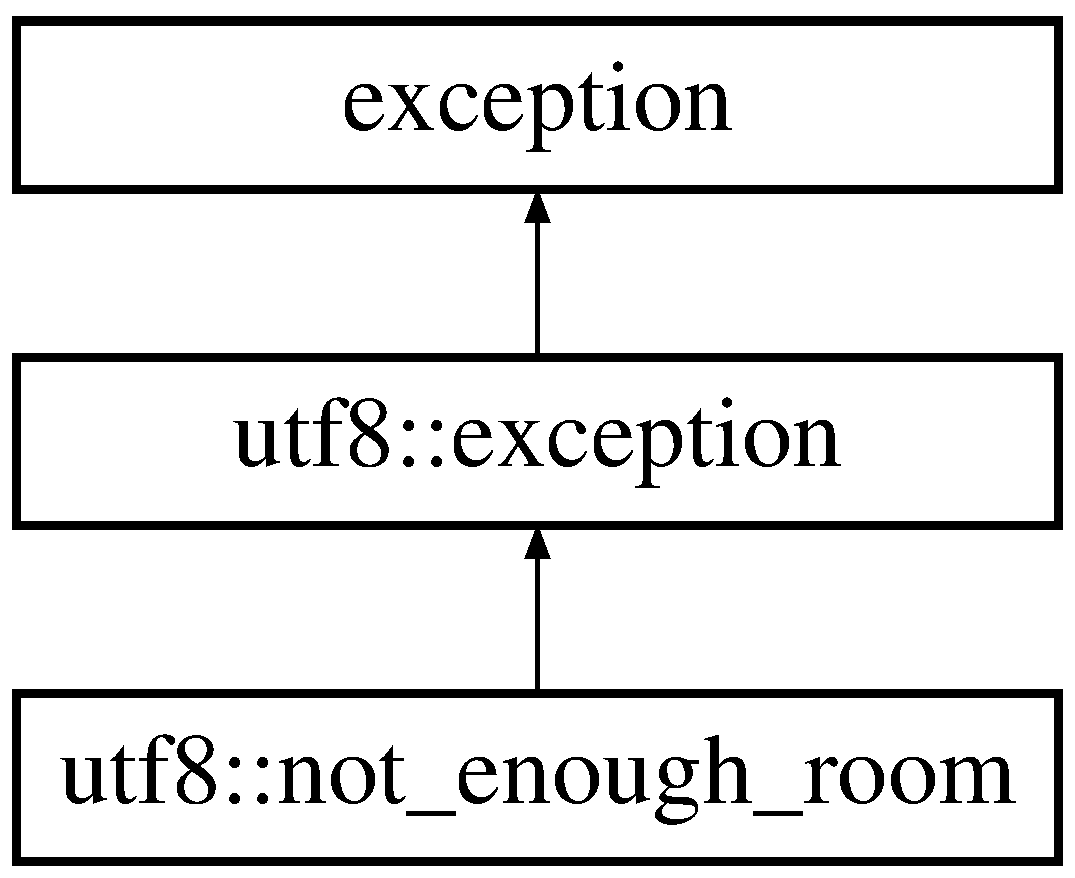
\includegraphics[height=3.000000cm]{classutf8_1_1not__enough__room}
\end{center}
\end{figure}
\subsection*{Public Member Functions}
\begin{DoxyCompactItemize}
\item 
virtual const char $\ast$ \hyperlink{classutf8_1_1not__enough__room_a368f7b33dc7d66e12576f55991c77676}{what} () const   throw ()
\end{DoxyCompactItemize}


\subsection{Member Function Documentation}
\hypertarget{classutf8_1_1not__enough__room_a368f7b33dc7d66e12576f55991c77676}{}\index{utf8\+::not\+\_\+enough\+\_\+room@{utf8\+::not\+\_\+enough\+\_\+room}!what@{what}}
\index{what@{what}!utf8\+::not\+\_\+enough\+\_\+room@{utf8\+::not\+\_\+enough\+\_\+room}}
\subsubsection[{what}]{\setlength{\rightskip}{0pt plus 5cm}virtual const char$\ast$ utf8\+::not\+\_\+enough\+\_\+room\+::what (
\begin{DoxyParamCaption}
{}
\end{DoxyParamCaption}
) const throw  ) \hspace{0.3cm}{\ttfamily [inline]}, {\ttfamily [virtual]}}\label{classutf8_1_1not__enough__room_a368f7b33dc7d66e12576f55991c77676}


The documentation for this class was generated from the following file\+:\begin{DoxyCompactItemize}
\item 
C\+:/cygwin/home/\+Engineer/\+Development/time-\/clock-\/front/\+Q\+B\+Wrapper/\+U\+T\+F-\/8/utf8/\hyperlink{checked_8h}{checked.\+h}\end{DoxyCompactItemize}

\hypertarget{structparam_data}{}\section{param\+Data Struct Reference}
\label{structparam_data}\index{param\+Data@{param\+Data}}


{\ttfamily \#include $<$Q\+B\+Wrapper.\+h$>$}

\subsection*{Public Attributes}
\begin{DoxyCompactItemize}
\item 
vector$<$ string $>$ \hyperlink{structparam_data_a2601bc4a92cb63714403a3cac4d55cfa}{b\+Params} = \{\}
\item 
vector$<$ string $>$ \hyperlink{structparam_data_ab973b0f2e408f0075b474e94f0b62fc5}{i\+Params} = \{\}
\item 
vector$<$ string $>$ \hyperlink{structparam_data_a19da62f881dccbf0f63c423e896ad8d1}{s\+Params} = \{\}
\item 
vector$<$ string $>$ \hyperlink{structparam_data_a645656536b9d6a8f716effeae49acbab}{f\+Params} = \{\}
\item 
vector$<$ bool $>$ \hyperlink{structparam_data_a0e70736d8fef01a994cb6282dcdcfc54}{b\+Values} = \{\}
\item 
vector$<$ int $>$ \hyperlink{structparam_data_a524931886354bfbd088178860999f9e1}{i\+Values} = \{\}
\item 
vector$<$ string $>$ \hyperlink{structparam_data_a530e1ec7867fb4713b34a1dfa0cffe14}{s\+Values} = \{\}
\item 
vector$<$ float $>$ \hyperlink{structparam_data_aded9de47eea4d3861aed3c649511648d}{f\+Values} = \{\}
\end{DoxyCompactItemize}


\subsection{Member Data Documentation}
\hypertarget{structparam_data_a2601bc4a92cb63714403a3cac4d55cfa}{}\index{param\+Data@{param\+Data}!b\+Params@{b\+Params}}
\index{b\+Params@{b\+Params}!param\+Data@{param\+Data}}
\subsubsection[{b\+Params}]{\setlength{\rightskip}{0pt plus 5cm}vector$<$string$>$ param\+Data\+::b\+Params = \{\}}\label{structparam_data_a2601bc4a92cb63714403a3cac4d55cfa}
\hypertarget{structparam_data_a0e70736d8fef01a994cb6282dcdcfc54}{}\index{param\+Data@{param\+Data}!b\+Values@{b\+Values}}
\index{b\+Values@{b\+Values}!param\+Data@{param\+Data}}
\subsubsection[{b\+Values}]{\setlength{\rightskip}{0pt plus 5cm}vector$<$bool$>$ param\+Data\+::b\+Values = \{\}}\label{structparam_data_a0e70736d8fef01a994cb6282dcdcfc54}
\hypertarget{structparam_data_a645656536b9d6a8f716effeae49acbab}{}\index{param\+Data@{param\+Data}!f\+Params@{f\+Params}}
\index{f\+Params@{f\+Params}!param\+Data@{param\+Data}}
\subsubsection[{f\+Params}]{\setlength{\rightskip}{0pt plus 5cm}vector$<$string$>$ param\+Data\+::f\+Params = \{\}}\label{structparam_data_a645656536b9d6a8f716effeae49acbab}
\hypertarget{structparam_data_aded9de47eea4d3861aed3c649511648d}{}\index{param\+Data@{param\+Data}!f\+Values@{f\+Values}}
\index{f\+Values@{f\+Values}!param\+Data@{param\+Data}}
\subsubsection[{f\+Values}]{\setlength{\rightskip}{0pt plus 5cm}vector$<$float$>$ param\+Data\+::f\+Values = \{\}}\label{structparam_data_aded9de47eea4d3861aed3c649511648d}
\hypertarget{structparam_data_ab973b0f2e408f0075b474e94f0b62fc5}{}\index{param\+Data@{param\+Data}!i\+Params@{i\+Params}}
\index{i\+Params@{i\+Params}!param\+Data@{param\+Data}}
\subsubsection[{i\+Params}]{\setlength{\rightskip}{0pt plus 5cm}vector$<$string$>$ param\+Data\+::i\+Params = \{\}}\label{structparam_data_ab973b0f2e408f0075b474e94f0b62fc5}
\hypertarget{structparam_data_a524931886354bfbd088178860999f9e1}{}\index{param\+Data@{param\+Data}!i\+Values@{i\+Values}}
\index{i\+Values@{i\+Values}!param\+Data@{param\+Data}}
\subsubsection[{i\+Values}]{\setlength{\rightskip}{0pt plus 5cm}vector$<$int$>$ param\+Data\+::i\+Values = \{\}}\label{structparam_data_a524931886354bfbd088178860999f9e1}
\hypertarget{structparam_data_a19da62f881dccbf0f63c423e896ad8d1}{}\index{param\+Data@{param\+Data}!s\+Params@{s\+Params}}
\index{s\+Params@{s\+Params}!param\+Data@{param\+Data}}
\subsubsection[{s\+Params}]{\setlength{\rightskip}{0pt plus 5cm}vector$<$string$>$ param\+Data\+::s\+Params = \{\}}\label{structparam_data_a19da62f881dccbf0f63c423e896ad8d1}
\hypertarget{structparam_data_a530e1ec7867fb4713b34a1dfa0cffe14}{}\index{param\+Data@{param\+Data}!s\+Values@{s\+Values}}
\index{s\+Values@{s\+Values}!param\+Data@{param\+Data}}
\subsubsection[{s\+Values}]{\setlength{\rightskip}{0pt plus 5cm}vector$<$string$>$ param\+Data\+::s\+Values = \{\}}\label{structparam_data_a530e1ec7867fb4713b34a1dfa0cffe14}


The documentation for this struct was generated from the following file\+:\begin{DoxyCompactItemize}
\item 
C\+:/cygwin/home/\+Engineer/\+Development/time-\/clock-\/front/\+Q\+B\+Wrapper/\hyperlink{_q_b_wrapper_8h}{Q\+B\+Wrapper.\+h}\end{DoxyCompactItemize}

\hypertarget{class_q_b_wrapper}{}\section{Q\+B\+Wrapper Class Reference}
\label{class_q_b_wrapper}\index{Q\+B\+Wrapper@{Q\+B\+Wrapper}}


{\ttfamily \#include $<$Q\+B\+Wrapper.\+h$>$}

\subsection*{Public Member Functions}
\begin{DoxyCompactItemize}
\item 
\hyperlink{class_q_b_wrapper_af53be4336b122a01f5fe4731e1ac612a}{Q\+B\+Wrapper} ()
\item 
\hyperlink{class_q_b_wrapper_a68833457b1963e6cb888f39702d9d7df}{$\sim$\+Q\+B\+Wrapper} ()
\item 
void \hyperlink{class_q_b_wrapper_acb5c3565b3f0a4a6332b524d5b300b70}{Set\+App\+Location} (string location)
\item 
void \hyperlink{class_q_b_wrapper_a306867c866078edb73acd59235f8a417}{Set\+App\+Token} (string token)
\item 
\hyperlink{class_q_b_x_m_l}{Q\+B\+X\+M\+L} \hyperlink{class_q_b_wrapper_aeac0cd9c9c43c54fa0c965001b8361ac}{Authenticate} (string username, string password, int hours, string udata)
\item 
\hyperlink{class_q_b_x_m_l}{Q\+B\+X\+M\+L} \hyperlink{class_q_b_wrapper_ae7d56cc01f73dad3fc80871337336a66}{Add\+Record} (vector$<$ string $>$ fields, vector$<$ string $>$ field\+Contents, bool disprec, bool ignore\+Error, string ticket, string apptoken, string udata, bool ms\+In\+U\+T\+C, string dbid)
\item 
\hyperlink{class_q_b_x_m_l}{Q\+B\+X\+M\+L} \hyperlink{class_q_b_wrapper_a91a75b6d40df547582f8afac5bbc3da8}{Edit\+Record} (int rid, int update\+I\+D, vector$<$ string $>$ fields, vector$<$ string $>$ contents, bool disprec, bool ignore\+Error, string ticket, string apptoken, string udata, bool ms\+In\+U\+T\+C, string dbid)
\item 
\hyperlink{class_q_b_x_m_l}{Q\+B\+X\+M\+L} \hyperlink{class_q_b_wrapper_a8f525eba166a9ead5b945a4d4a35d0a6}{Get\+Schema} (string ticket, string apptoken, string udata, string dbid)
\item 
\hyperlink{class_q_b_x_m_l}{Q\+B\+X\+M\+L} \hyperlink{class_q_b_wrapper_a1b584e685675bc48e1084a84d6db0dd9}{Get\+D\+B\+Info} (string ticket, string apptoken, string udata, string dbid)
\item 
\hyperlink{class_q_b_x_m_l}{Q\+B\+X\+M\+L} \hyperlink{class_q_b_wrapper_a411e4f414a4ff74801720da3502c4f33}{Add\+Field} (bool add\+To\+Forms, string apptoken, string label, string mode, string ticket, string type, string udata, string dbid)
\item 
\hyperlink{class_q_b_x_m_l}{Q\+B\+X\+M\+L} \hyperlink{class_q_b_wrapper_aa05817f83b2a60cc31bc5350399e1d89}{Delete\+Field} (int fid, string ticket, string apptoken, string udata, string dbid)
\item 
\hyperlink{class_q_b_x_m_l}{Q\+B\+X\+M\+L} \hyperlink{class_q_b_wrapper_adbdd00c2d8e49a47f4f04eed85240068}{Set\+Field\+Properties} (vector$<$ string $>$property\+Params, vector$<$ string $>$property\+Values, int fid, string ticket, string apptoken, string udata, string dbid)
\item 
\hyperlink{class_q_b_x_m_l}{Q\+B\+X\+M\+L} \hyperlink{class_q_b_wrapper_a2f113126a6be90cf7e6989d88fd552a4}{Create\+Table} (string tname, string pnoun, string ticket, string apptoken, string udata, string dbid)
\item 
\hyperlink{class_q_b_x_m_l}{Q\+B\+X\+M\+L} \hyperlink{class_q_b_wrapper_ae2683af81b7d67ed63ba488760506285}{Get\+Num\+Records} (string ticket, string apptoken, string udata, string dbid)
\item 
\hyperlink{class_q_b_x_m_l}{Q\+B\+X\+M\+L} \hyperlink{class_q_b_wrapper_a0489d9d624cc4bde429f20facc15d3d6}{Get\+Record\+Info} (int rid, string ticket, string apptoken, string udata, string dbid)
\item 
\hyperlink{class_q_b_x_m_l}{Q\+B\+X\+M\+L} \hyperlink{class_q_b_wrapper_affa5d7c3f1a19d0509d2a5c03e7b2c8f}{Delete\+Record} (int rid, string ticket, string apptoken, string udata, string dbid)
\item 
\hyperlink{class_q_b_x_m_l}{Q\+B\+X\+M\+L} \hyperlink{class_q_b_wrapper_a563d79fecd24b0ddae2be0a36c27e448}{Purge\+Records} (string query, int qid, string qname, string ticket, string apptoken, string udata, string dbid)
\item 
\hyperlink{class_q_b_x_m_l}{Q\+B\+X\+M\+L} \hyperlink{class_q_b_wrapper_ad75e2cd8fe5541a317e0b07e6a130aeb}{Do\+Query} (string query, int qid, string qname, string clist, string slist, bool fmt, bool return\+Percentage, string options, bool include\+Rids, string ticket, string apptoken, string udata, string dbid)
\item 
string \hyperlink{class_q_b_wrapper_a31b1f95cf4507b683a584bd9345f025d}{Get\+Field\+Contents} (int fid, string ticket, string apptoken, string udata, string dbid, int rid)
\item 
void \hyperlink{class_q_b_wrapper_a23f67ceee52901ab538998f9bfe3b167}{Cleanup} ()
\end{DoxyCompactItemize}


\subsection{Constructor \& Destructor Documentation}
\hypertarget{class_q_b_wrapper_af53be4336b122a01f5fe4731e1ac612a}{}\index{Q\+B\+Wrapper@{Q\+B\+Wrapper}!Q\+B\+Wrapper@{Q\+B\+Wrapper}}
\index{Q\+B\+Wrapper@{Q\+B\+Wrapper}!Q\+B\+Wrapper@{Q\+B\+Wrapper}}
\subsubsection[{Q\+B\+Wrapper}]{\setlength{\rightskip}{0pt plus 5cm}Q\+B\+Wrapper\+::\+Q\+B\+Wrapper (
\begin{DoxyParamCaption}
{}
\end{DoxyParamCaption}
)}\label{class_q_b_wrapper_af53be4336b122a01f5fe4731e1ac612a}
\hypertarget{class_q_b_wrapper_a68833457b1963e6cb888f39702d9d7df}{}\index{Q\+B\+Wrapper@{Q\+B\+Wrapper}!````~Q\+B\+Wrapper@{$\sim$\+Q\+B\+Wrapper}}
\index{````~Q\+B\+Wrapper@{$\sim$\+Q\+B\+Wrapper}!Q\+B\+Wrapper@{Q\+B\+Wrapper}}
\subsubsection[{$\sim$\+Q\+B\+Wrapper}]{\setlength{\rightskip}{0pt plus 5cm}Q\+B\+Wrapper\+::$\sim$\+Q\+B\+Wrapper (
\begin{DoxyParamCaption}
{}
\end{DoxyParamCaption}
)}\label{class_q_b_wrapper_a68833457b1963e6cb888f39702d9d7df}


\subsection{Member Function Documentation}
\hypertarget{class_q_b_wrapper_a411e4f414a4ff74801720da3502c4f33}{}\index{Q\+B\+Wrapper@{Q\+B\+Wrapper}!Add\+Field@{Add\+Field}}
\index{Add\+Field@{Add\+Field}!Q\+B\+Wrapper@{Q\+B\+Wrapper}}
\subsubsection[{Add\+Field}]{\setlength{\rightskip}{0pt plus 5cm}{\bf Q\+B\+X\+M\+L} Q\+B\+Wrapper\+::\+Add\+Field (
\begin{DoxyParamCaption}
\item[{bool}]{add\+To\+Forms, }
\item[{string}]{apptoken, }
\item[{string}]{label, }
\item[{string}]{mode, }
\item[{string}]{ticket, }
\item[{string}]{type, }
\item[{string}]{udata, }
\item[{string}]{dbid}
\end{DoxyParamCaption}
)}\label{class_q_b_wrapper_a411e4f414a4ff74801720da3502c4f33}
\hypertarget{class_q_b_wrapper_ae7d56cc01f73dad3fc80871337336a66}{}\index{Q\+B\+Wrapper@{Q\+B\+Wrapper}!Add\+Record@{Add\+Record}}
\index{Add\+Record@{Add\+Record}!Q\+B\+Wrapper@{Q\+B\+Wrapper}}
\subsubsection[{Add\+Record}]{\setlength{\rightskip}{0pt plus 5cm}{\bf Q\+B\+X\+M\+L} Q\+B\+Wrapper\+::\+Add\+Record (
\begin{DoxyParamCaption}
\item[{vector$<$ string $>$}]{fields, }
\item[{vector$<$ string $>$}]{field\+Contents, }
\item[{bool}]{disprec, }
\item[{bool}]{ignore\+Error, }
\item[{string}]{ticket, }
\item[{string}]{apptoken, }
\item[{string}]{udata, }
\item[{bool}]{ms\+In\+U\+T\+C, }
\item[{string}]{dbid}
\end{DoxyParamCaption}
)}\label{class_q_b_wrapper_ae7d56cc01f73dad3fc80871337336a66}
\hypertarget{class_q_b_wrapper_aeac0cd9c9c43c54fa0c965001b8361ac}{}\index{Q\+B\+Wrapper@{Q\+B\+Wrapper}!Authenticate@{Authenticate}}
\index{Authenticate@{Authenticate}!Q\+B\+Wrapper@{Q\+B\+Wrapper}}
\subsubsection[{Authenticate}]{\setlength{\rightskip}{0pt plus 5cm}{\bf Q\+B\+X\+M\+L} Q\+B\+Wrapper\+::\+Authenticate (
\begin{DoxyParamCaption}
\item[{string}]{username, }
\item[{string}]{password, }
\item[{int}]{hours, }
\item[{string}]{udata}
\end{DoxyParamCaption}
)}\label{class_q_b_wrapper_aeac0cd9c9c43c54fa0c965001b8361ac}
\hypertarget{class_q_b_wrapper_a23f67ceee52901ab538998f9bfe3b167}{}\index{Q\+B\+Wrapper@{Q\+B\+Wrapper}!Cleanup@{Cleanup}}
\index{Cleanup@{Cleanup}!Q\+B\+Wrapper@{Q\+B\+Wrapper}}
\subsubsection[{Cleanup}]{\setlength{\rightskip}{0pt plus 5cm}void Q\+B\+Wrapper\+::\+Cleanup (
\begin{DoxyParamCaption}
{}
\end{DoxyParamCaption}
)}\label{class_q_b_wrapper_a23f67ceee52901ab538998f9bfe3b167}
\hypertarget{class_q_b_wrapper_a2f113126a6be90cf7e6989d88fd552a4}{}\index{Q\+B\+Wrapper@{Q\+B\+Wrapper}!Create\+Table@{Create\+Table}}
\index{Create\+Table@{Create\+Table}!Q\+B\+Wrapper@{Q\+B\+Wrapper}}
\subsubsection[{Create\+Table}]{\setlength{\rightskip}{0pt plus 5cm}{\bf Q\+B\+X\+M\+L} Q\+B\+Wrapper\+::\+Create\+Table (
\begin{DoxyParamCaption}
\item[{string}]{tname, }
\item[{string}]{pnoun, }
\item[{string}]{ticket, }
\item[{string}]{apptoken, }
\item[{string}]{udata, }
\item[{string}]{dbid}
\end{DoxyParamCaption}
)}\label{class_q_b_wrapper_a2f113126a6be90cf7e6989d88fd552a4}
\hypertarget{class_q_b_wrapper_aa05817f83b2a60cc31bc5350399e1d89}{}\index{Q\+B\+Wrapper@{Q\+B\+Wrapper}!Delete\+Field@{Delete\+Field}}
\index{Delete\+Field@{Delete\+Field}!Q\+B\+Wrapper@{Q\+B\+Wrapper}}
\subsubsection[{Delete\+Field}]{\setlength{\rightskip}{0pt plus 5cm}{\bf Q\+B\+X\+M\+L} Q\+B\+Wrapper\+::\+Delete\+Field (
\begin{DoxyParamCaption}
\item[{int}]{fid, }
\item[{string}]{ticket, }
\item[{string}]{apptoken, }
\item[{string}]{udata, }
\item[{string}]{dbid}
\end{DoxyParamCaption}
)}\label{class_q_b_wrapper_aa05817f83b2a60cc31bc5350399e1d89}
\hypertarget{class_q_b_wrapper_affa5d7c3f1a19d0509d2a5c03e7b2c8f}{}\index{Q\+B\+Wrapper@{Q\+B\+Wrapper}!Delete\+Record@{Delete\+Record}}
\index{Delete\+Record@{Delete\+Record}!Q\+B\+Wrapper@{Q\+B\+Wrapper}}
\subsubsection[{Delete\+Record}]{\setlength{\rightskip}{0pt plus 5cm}{\bf Q\+B\+X\+M\+L} Q\+B\+Wrapper\+::\+Delete\+Record (
\begin{DoxyParamCaption}
\item[{int}]{rid, }
\item[{string}]{ticket, }
\item[{string}]{apptoken, }
\item[{string}]{udata, }
\item[{string}]{dbid}
\end{DoxyParamCaption}
)}\label{class_q_b_wrapper_affa5d7c3f1a19d0509d2a5c03e7b2c8f}
\hypertarget{class_q_b_wrapper_ad75e2cd8fe5541a317e0b07e6a130aeb}{}\index{Q\+B\+Wrapper@{Q\+B\+Wrapper}!Do\+Query@{Do\+Query}}
\index{Do\+Query@{Do\+Query}!Q\+B\+Wrapper@{Q\+B\+Wrapper}}
\subsubsection[{Do\+Query}]{\setlength{\rightskip}{0pt plus 5cm}{\bf Q\+B\+X\+M\+L} Q\+B\+Wrapper\+::\+Do\+Query (
\begin{DoxyParamCaption}
\item[{string}]{query, }
\item[{int}]{qid, }
\item[{string}]{qname, }
\item[{string}]{clist, }
\item[{string}]{slist, }
\item[{bool}]{fmt, }
\item[{bool}]{return\+Percentage, }
\item[{string}]{options, }
\item[{bool}]{include\+Rids, }
\item[{string}]{ticket, }
\item[{string}]{apptoken, }
\item[{string}]{udata, }
\item[{string}]{dbid}
\end{DoxyParamCaption}
)}\label{class_q_b_wrapper_ad75e2cd8fe5541a317e0b07e6a130aeb}
\hypertarget{class_q_b_wrapper_a91a75b6d40df547582f8afac5bbc3da8}{}\index{Q\+B\+Wrapper@{Q\+B\+Wrapper}!Edit\+Record@{Edit\+Record}}
\index{Edit\+Record@{Edit\+Record}!Q\+B\+Wrapper@{Q\+B\+Wrapper}}
\subsubsection[{Edit\+Record}]{\setlength{\rightskip}{0pt plus 5cm}{\bf Q\+B\+X\+M\+L} Q\+B\+Wrapper\+::\+Edit\+Record (
\begin{DoxyParamCaption}
\item[{int}]{rid, }
\item[{int}]{update\+I\+D, }
\item[{vector$<$ string $>$}]{fields, }
\item[{vector$<$ string $>$}]{contents, }
\item[{bool}]{disprec, }
\item[{bool}]{ignore\+Error, }
\item[{string}]{ticket, }
\item[{string}]{apptoken, }
\item[{string}]{udata, }
\item[{bool}]{ms\+In\+U\+T\+C, }
\item[{string}]{dbid}
\end{DoxyParamCaption}
)}\label{class_q_b_wrapper_a91a75b6d40df547582f8afac5bbc3da8}
\hypertarget{class_q_b_wrapper_a1b584e685675bc48e1084a84d6db0dd9}{}\index{Q\+B\+Wrapper@{Q\+B\+Wrapper}!Get\+D\+B\+Info@{Get\+D\+B\+Info}}
\index{Get\+D\+B\+Info@{Get\+D\+B\+Info}!Q\+B\+Wrapper@{Q\+B\+Wrapper}}
\subsubsection[{Get\+D\+B\+Info}]{\setlength{\rightskip}{0pt plus 5cm}{\bf Q\+B\+X\+M\+L} Q\+B\+Wrapper\+::\+Get\+D\+B\+Info (
\begin{DoxyParamCaption}
\item[{string}]{ticket, }
\item[{string}]{apptoken, }
\item[{string}]{udata, }
\item[{string}]{dbid}
\end{DoxyParamCaption}
)}\label{class_q_b_wrapper_a1b584e685675bc48e1084a84d6db0dd9}
\hypertarget{class_q_b_wrapper_a31b1f95cf4507b683a584bd9345f025d}{}\index{Q\+B\+Wrapper@{Q\+B\+Wrapper}!Get\+Field\+Contents@{Get\+Field\+Contents}}
\index{Get\+Field\+Contents@{Get\+Field\+Contents}!Q\+B\+Wrapper@{Q\+B\+Wrapper}}
\subsubsection[{Get\+Field\+Contents}]{\setlength{\rightskip}{0pt plus 5cm}string Q\+B\+Wrapper\+::\+Get\+Field\+Contents (
\begin{DoxyParamCaption}
\item[{int}]{fid, }
\item[{string}]{ticket, }
\item[{string}]{apptoken, }
\item[{string}]{udata, }
\item[{string}]{dbid, }
\item[{int}]{rid}
\end{DoxyParamCaption}
)}\label{class_q_b_wrapper_a31b1f95cf4507b683a584bd9345f025d}
\hypertarget{class_q_b_wrapper_ae2683af81b7d67ed63ba488760506285}{}\index{Q\+B\+Wrapper@{Q\+B\+Wrapper}!Get\+Num\+Records@{Get\+Num\+Records}}
\index{Get\+Num\+Records@{Get\+Num\+Records}!Q\+B\+Wrapper@{Q\+B\+Wrapper}}
\subsubsection[{Get\+Num\+Records}]{\setlength{\rightskip}{0pt plus 5cm}{\bf Q\+B\+X\+M\+L} Q\+B\+Wrapper\+::\+Get\+Num\+Records (
\begin{DoxyParamCaption}
\item[{string}]{ticket, }
\item[{string}]{apptoken, }
\item[{string}]{udata, }
\item[{string}]{dbid}
\end{DoxyParamCaption}
)}\label{class_q_b_wrapper_ae2683af81b7d67ed63ba488760506285}
\hypertarget{class_q_b_wrapper_a0489d9d624cc4bde429f20facc15d3d6}{}\index{Q\+B\+Wrapper@{Q\+B\+Wrapper}!Get\+Record\+Info@{Get\+Record\+Info}}
\index{Get\+Record\+Info@{Get\+Record\+Info}!Q\+B\+Wrapper@{Q\+B\+Wrapper}}
\subsubsection[{Get\+Record\+Info}]{\setlength{\rightskip}{0pt plus 5cm}{\bf Q\+B\+X\+M\+L} Q\+B\+Wrapper\+::\+Get\+Record\+Info (
\begin{DoxyParamCaption}
\item[{int}]{rid, }
\item[{string}]{ticket, }
\item[{string}]{apptoken, }
\item[{string}]{udata, }
\item[{string}]{dbid}
\end{DoxyParamCaption}
)}\label{class_q_b_wrapper_a0489d9d624cc4bde429f20facc15d3d6}
\hypertarget{class_q_b_wrapper_a8f525eba166a9ead5b945a4d4a35d0a6}{}\index{Q\+B\+Wrapper@{Q\+B\+Wrapper}!Get\+Schema@{Get\+Schema}}
\index{Get\+Schema@{Get\+Schema}!Q\+B\+Wrapper@{Q\+B\+Wrapper}}
\subsubsection[{Get\+Schema}]{\setlength{\rightskip}{0pt plus 5cm}{\bf Q\+B\+X\+M\+L} Q\+B\+Wrapper\+::\+Get\+Schema (
\begin{DoxyParamCaption}
\item[{string}]{ticket, }
\item[{string}]{apptoken, }
\item[{string}]{udata, }
\item[{string}]{dbid}
\end{DoxyParamCaption}
)}\label{class_q_b_wrapper_a8f525eba166a9ead5b945a4d4a35d0a6}
\hypertarget{class_q_b_wrapper_a563d79fecd24b0ddae2be0a36c27e448}{}\index{Q\+B\+Wrapper@{Q\+B\+Wrapper}!Purge\+Records@{Purge\+Records}}
\index{Purge\+Records@{Purge\+Records}!Q\+B\+Wrapper@{Q\+B\+Wrapper}}
\subsubsection[{Purge\+Records}]{\setlength{\rightskip}{0pt plus 5cm}{\bf Q\+B\+X\+M\+L} Q\+B\+Wrapper\+::\+Purge\+Records (
\begin{DoxyParamCaption}
\item[{string}]{query, }
\item[{int}]{qid, }
\item[{string}]{qname, }
\item[{string}]{ticket, }
\item[{string}]{apptoken, }
\item[{string}]{udata, }
\item[{string}]{dbid}
\end{DoxyParamCaption}
)}\label{class_q_b_wrapper_a563d79fecd24b0ddae2be0a36c27e448}
\hypertarget{class_q_b_wrapper_acb5c3565b3f0a4a6332b524d5b300b70}{}\index{Q\+B\+Wrapper@{Q\+B\+Wrapper}!Set\+App\+Location@{Set\+App\+Location}}
\index{Set\+App\+Location@{Set\+App\+Location}!Q\+B\+Wrapper@{Q\+B\+Wrapper}}
\subsubsection[{Set\+App\+Location}]{\setlength{\rightskip}{0pt plus 5cm}void Q\+B\+Wrapper\+::\+Set\+App\+Location (
\begin{DoxyParamCaption}
\item[{string}]{location}
\end{DoxyParamCaption}
)}\label{class_q_b_wrapper_acb5c3565b3f0a4a6332b524d5b300b70}
\hypertarget{class_q_b_wrapper_a306867c866078edb73acd59235f8a417}{}\index{Q\+B\+Wrapper@{Q\+B\+Wrapper}!Set\+App\+Token@{Set\+App\+Token}}
\index{Set\+App\+Token@{Set\+App\+Token}!Q\+B\+Wrapper@{Q\+B\+Wrapper}}
\subsubsection[{Set\+App\+Token}]{\setlength{\rightskip}{0pt plus 5cm}void Q\+B\+Wrapper\+::\+Set\+App\+Token (
\begin{DoxyParamCaption}
\item[{string}]{token}
\end{DoxyParamCaption}
)}\label{class_q_b_wrapper_a306867c866078edb73acd59235f8a417}
\hypertarget{class_q_b_wrapper_adbdd00c2d8e49a47f4f04eed85240068}{}\index{Q\+B\+Wrapper@{Q\+B\+Wrapper}!Set\+Field\+Properties@{Set\+Field\+Properties}}
\index{Set\+Field\+Properties@{Set\+Field\+Properties}!Q\+B\+Wrapper@{Q\+B\+Wrapper}}
\subsubsection[{Set\+Field\+Properties}]{\setlength{\rightskip}{0pt plus 5cm}{\bf Q\+B\+X\+M\+L} Q\+B\+Wrapper\+::\+Set\+Field\+Properties (
\begin{DoxyParamCaption}
\item[{vector$<$ string $>$}]{property\+Params, }
\item[{vector$<$ string $>$}]{property\+Values, }
\item[{int}]{fid, }
\item[{string}]{ticket, }
\item[{string}]{apptoken, }
\item[{string}]{udata, }
\item[{string}]{dbid}
\end{DoxyParamCaption}
)}\label{class_q_b_wrapper_adbdd00c2d8e49a47f4f04eed85240068}


The documentation for this class was generated from the following files\+:\begin{DoxyCompactItemize}
\item 
C\+:/cygwin/home/\+Engineer/\+Development/time-\/clock-\/front/\+Q\+B\+Wrapper/\hyperlink{_q_b_wrapper_8h}{Q\+B\+Wrapper.\+h}\item 
C\+:/cygwin/home/\+Engineer/\+Development/time-\/clock-\/front/\+Q\+B\+Wrapper/\hyperlink{_q_b_wrapper_8cpp}{Q\+B\+Wrapper.\+cpp}\end{DoxyCompactItemize}

\hypertarget{class_q_b_x_m_l}{}\section{Q\+B\+X\+M\+L Class Reference}
\label{class_q_b_x_m_l}\index{Q\+B\+X\+M\+L@{Q\+B\+X\+M\+L}}


{\ttfamily \#include $<$Q\+B\+X\+M\+L.\+h$>$}

\subsection*{Public Member Functions}
\begin{DoxyCompactItemize}
\item 
\hyperlink{class_q_b_x_m_l_ad5d7e15c9c1d968f57e681e7c5cb6c04}{Q\+B\+X\+M\+L} (\hyperlink{class_x_m_l_read}{X\+M\+L\+Read} $\ast$read)
\item 
\hyperlink{class_q_b_x_m_l_a29b25b0d79351ec8498aeca770cf854f}{$\sim$\+Q\+B\+X\+M\+L} ()
\item 
void \hyperlink{class_q_b_x_m_l_a146d1f5ee8f24fce540eb1c1f4c20ee9}{Dealloc} ()
\item 
\hyperlink{struct_x_m_l_result}{X\+M\+L\+Result} \hyperlink{class_q_b_x_m_l_a7a110dde5772b961ca6c572b4caaca8b}{Get\+Action} ()
\item 
\hyperlink{struct_x_m_l_result}{X\+M\+L\+Result} \hyperlink{class_q_b_x_m_l_a0acf0bdc0f8b865d9016510057816ecf}{Get\+Err\+Code} ()
\item 
\hyperlink{struct_x_m_l_result}{X\+M\+L\+Result} \hyperlink{class_q_b_x_m_l_a77cd91afd92fe8fe4861269eabed85e8}{Get\+Err\+Text} ()
\item 
\hyperlink{struct_x_m_l_result}{X\+M\+L\+Result} \hyperlink{class_q_b_x_m_l_a58b44d06a90f3a0012d0c3e77b30720c}{Get\+U\+Data} ()
\item 
\hyperlink{struct_x_m_l_result}{X\+M\+L\+Result} \hyperlink{class_q_b_x_m_l_ae8f688578c62d3e12939c0a1d7246073}{Get\+User\+I\+D} ()
\item 
\hyperlink{struct_x_m_l_result}{X\+M\+L\+Result} \hyperlink{class_q_b_x_m_l_ac0fc9a0151377c29c8c2f864aef82ff7}{Get\+Ticket} ()
\item 
\hyperlink{struct_x_m_l_result}{X\+M\+L\+Result} \hyperlink{class_q_b_x_m_l_a08fa0b97fcc3feac3b41db1ce3aa1d37}{Get\+R\+I\+D} ()
\item 
\hyperlink{struct_x_m_l_result}{X\+M\+L\+Result} \hyperlink{class_q_b_x_m_l_a014c3f5b93eac9afaa2c6815a35c2583}{Get\+Update\+I\+D} ()
\item 
\hyperlink{struct_x_m_l_result}{X\+M\+L\+Result} \hyperlink{class_q_b_x_m_l_a1f8ba59f5ee8ff09c0bfee29586c92d6}{Get\+F\+I\+D} ()
\item 
\hyperlink{struct_x_m_l_result}{X\+M\+L\+Result} \hyperlink{class_q_b_x_m_l_aec4f1f6a57b4a0818ef1bb031fa931e4}{Get\+Label} ()
\item 
\hyperlink{struct_x_m_l_result}{X\+M\+L\+Result} \hyperlink{class_q_b_x_m_l_af6574482722aa1369cfb5f3b3dd1fdd3}{Get\+Num\+Fields\+Changed} ()
\item 
\hyperlink{struct_x_m_l_result}{X\+M\+L\+Result} \hyperlink{class_q_b_x_m_l_aca2882b34f865a22e512ffd291c99202}{Get\+New\+D\+B\+I\+D} ()
\item 
\hyperlink{struct_x_m_l_result}{X\+M\+L\+Result} \hyperlink{class_q_b_x_m_l_ab0bba404c8b07ee490f719f4d8d6d04b}{Get\+Record} ()
\item 
\hyperlink{struct_x_m_l_result}{X\+M\+L\+Result} \hyperlink{class_q_b_x_m_l_a9117678ee7676294fee4b3a85bebb54b}{Get\+Num\+Fields} ()
\item 
\hyperlink{struct_x_m_l_result}{X\+M\+L\+Result} \hyperlink{class_q_b_x_m_l_ac30e2951aa89b481fa02859fe6275265}{Get\+Value} ()
\item 
vector$<$ \hyperlink{class_q_b_x_m_l}{Q\+B\+X\+M\+L} $>$ \hyperlink{class_q_b_x_m_l_ab108326c6f1af5b853cbd2c0d58d5316}{Get\+Fields} ()
\end{DoxyCompactItemize}


\subsection{Constructor \& Destructor Documentation}
\hypertarget{class_q_b_x_m_l_ad5d7e15c9c1d968f57e681e7c5cb6c04}{}\index{Q\+B\+X\+M\+L@{Q\+B\+X\+M\+L}!Q\+B\+X\+M\+L@{Q\+B\+X\+M\+L}}
\index{Q\+B\+X\+M\+L@{Q\+B\+X\+M\+L}!Q\+B\+X\+M\+L@{Q\+B\+X\+M\+L}}
\subsubsection[{Q\+B\+X\+M\+L}]{\setlength{\rightskip}{0pt plus 5cm}Q\+B\+X\+M\+L\+::\+Q\+B\+X\+M\+L (
\begin{DoxyParamCaption}
\item[{{\bf X\+M\+L\+Read} $\ast$}]{read}
\end{DoxyParamCaption}
)}\label{class_q_b_x_m_l_ad5d7e15c9c1d968f57e681e7c5cb6c04}
\hypertarget{class_q_b_x_m_l_a29b25b0d79351ec8498aeca770cf854f}{}\index{Q\+B\+X\+M\+L@{Q\+B\+X\+M\+L}!````~Q\+B\+X\+M\+L@{$\sim$\+Q\+B\+X\+M\+L}}
\index{````~Q\+B\+X\+M\+L@{$\sim$\+Q\+B\+X\+M\+L}!Q\+B\+X\+M\+L@{Q\+B\+X\+M\+L}}
\subsubsection[{$\sim$\+Q\+B\+X\+M\+L}]{\setlength{\rightskip}{0pt plus 5cm}Q\+B\+X\+M\+L\+::$\sim$\+Q\+B\+X\+M\+L (
\begin{DoxyParamCaption}
{}
\end{DoxyParamCaption}
)}\label{class_q_b_x_m_l_a29b25b0d79351ec8498aeca770cf854f}


\subsection{Member Function Documentation}
\hypertarget{class_q_b_x_m_l_a146d1f5ee8f24fce540eb1c1f4c20ee9}{}\index{Q\+B\+X\+M\+L@{Q\+B\+X\+M\+L}!Dealloc@{Dealloc}}
\index{Dealloc@{Dealloc}!Q\+B\+X\+M\+L@{Q\+B\+X\+M\+L}}
\subsubsection[{Dealloc}]{\setlength{\rightskip}{0pt plus 5cm}void Q\+B\+X\+M\+L\+::\+Dealloc (
\begin{DoxyParamCaption}
{}
\end{DoxyParamCaption}
)}\label{class_q_b_x_m_l_a146d1f5ee8f24fce540eb1c1f4c20ee9}
\hypertarget{class_q_b_x_m_l_a7a110dde5772b961ca6c572b4caaca8b}{}\index{Q\+B\+X\+M\+L@{Q\+B\+X\+M\+L}!Get\+Action@{Get\+Action}}
\index{Get\+Action@{Get\+Action}!Q\+B\+X\+M\+L@{Q\+B\+X\+M\+L}}
\subsubsection[{Get\+Action}]{\setlength{\rightskip}{0pt plus 5cm}{\bf X\+M\+L\+Result} Q\+B\+X\+M\+L\+::\+Get\+Action (
\begin{DoxyParamCaption}
{}
\end{DoxyParamCaption}
)}\label{class_q_b_x_m_l_a7a110dde5772b961ca6c572b4caaca8b}
\hypertarget{class_q_b_x_m_l_a0acf0bdc0f8b865d9016510057816ecf}{}\index{Q\+B\+X\+M\+L@{Q\+B\+X\+M\+L}!Get\+Err\+Code@{Get\+Err\+Code}}
\index{Get\+Err\+Code@{Get\+Err\+Code}!Q\+B\+X\+M\+L@{Q\+B\+X\+M\+L}}
\subsubsection[{Get\+Err\+Code}]{\setlength{\rightskip}{0pt plus 5cm}{\bf X\+M\+L\+Result} Q\+B\+X\+M\+L\+::\+Get\+Err\+Code (
\begin{DoxyParamCaption}
{}
\end{DoxyParamCaption}
)}\label{class_q_b_x_m_l_a0acf0bdc0f8b865d9016510057816ecf}
\hypertarget{class_q_b_x_m_l_a77cd91afd92fe8fe4861269eabed85e8}{}\index{Q\+B\+X\+M\+L@{Q\+B\+X\+M\+L}!Get\+Err\+Text@{Get\+Err\+Text}}
\index{Get\+Err\+Text@{Get\+Err\+Text}!Q\+B\+X\+M\+L@{Q\+B\+X\+M\+L}}
\subsubsection[{Get\+Err\+Text}]{\setlength{\rightskip}{0pt plus 5cm}{\bf X\+M\+L\+Result} Q\+B\+X\+M\+L\+::\+Get\+Err\+Text (
\begin{DoxyParamCaption}
{}
\end{DoxyParamCaption}
)}\label{class_q_b_x_m_l_a77cd91afd92fe8fe4861269eabed85e8}
\hypertarget{class_q_b_x_m_l_a1f8ba59f5ee8ff09c0bfee29586c92d6}{}\index{Q\+B\+X\+M\+L@{Q\+B\+X\+M\+L}!Get\+F\+I\+D@{Get\+F\+I\+D}}
\index{Get\+F\+I\+D@{Get\+F\+I\+D}!Q\+B\+X\+M\+L@{Q\+B\+X\+M\+L}}
\subsubsection[{Get\+F\+I\+D}]{\setlength{\rightskip}{0pt plus 5cm}{\bf X\+M\+L\+Result} Q\+B\+X\+M\+L\+::\+Get\+F\+I\+D (
\begin{DoxyParamCaption}
{}
\end{DoxyParamCaption}
)}\label{class_q_b_x_m_l_a1f8ba59f5ee8ff09c0bfee29586c92d6}
\hypertarget{class_q_b_x_m_l_ab108326c6f1af5b853cbd2c0d58d5316}{}\index{Q\+B\+X\+M\+L@{Q\+B\+X\+M\+L}!Get\+Fields@{Get\+Fields}}
\index{Get\+Fields@{Get\+Fields}!Q\+B\+X\+M\+L@{Q\+B\+X\+M\+L}}
\subsubsection[{Get\+Fields}]{\setlength{\rightskip}{0pt plus 5cm}vector$<$ {\bf Q\+B\+X\+M\+L} $>$ Q\+B\+X\+M\+L\+::\+Get\+Fields (
\begin{DoxyParamCaption}
{}
\end{DoxyParamCaption}
)}\label{class_q_b_x_m_l_ab108326c6f1af5b853cbd2c0d58d5316}
\hypertarget{class_q_b_x_m_l_aec4f1f6a57b4a0818ef1bb031fa931e4}{}\index{Q\+B\+X\+M\+L@{Q\+B\+X\+M\+L}!Get\+Label@{Get\+Label}}
\index{Get\+Label@{Get\+Label}!Q\+B\+X\+M\+L@{Q\+B\+X\+M\+L}}
\subsubsection[{Get\+Label}]{\setlength{\rightskip}{0pt plus 5cm}{\bf X\+M\+L\+Result} Q\+B\+X\+M\+L\+::\+Get\+Label (
\begin{DoxyParamCaption}
{}
\end{DoxyParamCaption}
)}\label{class_q_b_x_m_l_aec4f1f6a57b4a0818ef1bb031fa931e4}
\hypertarget{class_q_b_x_m_l_aca2882b34f865a22e512ffd291c99202}{}\index{Q\+B\+X\+M\+L@{Q\+B\+X\+M\+L}!Get\+New\+D\+B\+I\+D@{Get\+New\+D\+B\+I\+D}}
\index{Get\+New\+D\+B\+I\+D@{Get\+New\+D\+B\+I\+D}!Q\+B\+X\+M\+L@{Q\+B\+X\+M\+L}}
\subsubsection[{Get\+New\+D\+B\+I\+D}]{\setlength{\rightskip}{0pt plus 5cm}{\bf X\+M\+L\+Result} Q\+B\+X\+M\+L\+::\+Get\+New\+D\+B\+I\+D (
\begin{DoxyParamCaption}
{}
\end{DoxyParamCaption}
)}\label{class_q_b_x_m_l_aca2882b34f865a22e512ffd291c99202}
\hypertarget{class_q_b_x_m_l_a9117678ee7676294fee4b3a85bebb54b}{}\index{Q\+B\+X\+M\+L@{Q\+B\+X\+M\+L}!Get\+Num\+Fields@{Get\+Num\+Fields}}
\index{Get\+Num\+Fields@{Get\+Num\+Fields}!Q\+B\+X\+M\+L@{Q\+B\+X\+M\+L}}
\subsubsection[{Get\+Num\+Fields}]{\setlength{\rightskip}{0pt plus 5cm}{\bf X\+M\+L\+Result} Q\+B\+X\+M\+L\+::\+Get\+Num\+Fields (
\begin{DoxyParamCaption}
{}
\end{DoxyParamCaption}
)}\label{class_q_b_x_m_l_a9117678ee7676294fee4b3a85bebb54b}
\hypertarget{class_q_b_x_m_l_af6574482722aa1369cfb5f3b3dd1fdd3}{}\index{Q\+B\+X\+M\+L@{Q\+B\+X\+M\+L}!Get\+Num\+Fields\+Changed@{Get\+Num\+Fields\+Changed}}
\index{Get\+Num\+Fields\+Changed@{Get\+Num\+Fields\+Changed}!Q\+B\+X\+M\+L@{Q\+B\+X\+M\+L}}
\subsubsection[{Get\+Num\+Fields\+Changed}]{\setlength{\rightskip}{0pt plus 5cm}{\bf X\+M\+L\+Result} Q\+B\+X\+M\+L\+::\+Get\+Num\+Fields\+Changed (
\begin{DoxyParamCaption}
{}
\end{DoxyParamCaption}
)}\label{class_q_b_x_m_l_af6574482722aa1369cfb5f3b3dd1fdd3}
\hypertarget{class_q_b_x_m_l_ab0bba404c8b07ee490f719f4d8d6d04b}{}\index{Q\+B\+X\+M\+L@{Q\+B\+X\+M\+L}!Get\+Record@{Get\+Record}}
\index{Get\+Record@{Get\+Record}!Q\+B\+X\+M\+L@{Q\+B\+X\+M\+L}}
\subsubsection[{Get\+Record}]{\setlength{\rightskip}{0pt plus 5cm}{\bf X\+M\+L\+Result} Q\+B\+X\+M\+L\+::\+Get\+Record (
\begin{DoxyParamCaption}
{}
\end{DoxyParamCaption}
)}\label{class_q_b_x_m_l_ab0bba404c8b07ee490f719f4d8d6d04b}
\hypertarget{class_q_b_x_m_l_a08fa0b97fcc3feac3b41db1ce3aa1d37}{}\index{Q\+B\+X\+M\+L@{Q\+B\+X\+M\+L}!Get\+R\+I\+D@{Get\+R\+I\+D}}
\index{Get\+R\+I\+D@{Get\+R\+I\+D}!Q\+B\+X\+M\+L@{Q\+B\+X\+M\+L}}
\subsubsection[{Get\+R\+I\+D}]{\setlength{\rightskip}{0pt plus 5cm}{\bf X\+M\+L\+Result} Q\+B\+X\+M\+L\+::\+Get\+R\+I\+D (
\begin{DoxyParamCaption}
{}
\end{DoxyParamCaption}
)}\label{class_q_b_x_m_l_a08fa0b97fcc3feac3b41db1ce3aa1d37}
\hypertarget{class_q_b_x_m_l_ac0fc9a0151377c29c8c2f864aef82ff7}{}\index{Q\+B\+X\+M\+L@{Q\+B\+X\+M\+L}!Get\+Ticket@{Get\+Ticket}}
\index{Get\+Ticket@{Get\+Ticket}!Q\+B\+X\+M\+L@{Q\+B\+X\+M\+L}}
\subsubsection[{Get\+Ticket}]{\setlength{\rightskip}{0pt plus 5cm}{\bf X\+M\+L\+Result} Q\+B\+X\+M\+L\+::\+Get\+Ticket (
\begin{DoxyParamCaption}
{}
\end{DoxyParamCaption}
)}\label{class_q_b_x_m_l_ac0fc9a0151377c29c8c2f864aef82ff7}
\hypertarget{class_q_b_x_m_l_a58b44d06a90f3a0012d0c3e77b30720c}{}\index{Q\+B\+X\+M\+L@{Q\+B\+X\+M\+L}!Get\+U\+Data@{Get\+U\+Data}}
\index{Get\+U\+Data@{Get\+U\+Data}!Q\+B\+X\+M\+L@{Q\+B\+X\+M\+L}}
\subsubsection[{Get\+U\+Data}]{\setlength{\rightskip}{0pt plus 5cm}{\bf X\+M\+L\+Result} Q\+B\+X\+M\+L\+::\+Get\+U\+Data (
\begin{DoxyParamCaption}
{}
\end{DoxyParamCaption}
)}\label{class_q_b_x_m_l_a58b44d06a90f3a0012d0c3e77b30720c}
\hypertarget{class_q_b_x_m_l_a014c3f5b93eac9afaa2c6815a35c2583}{}\index{Q\+B\+X\+M\+L@{Q\+B\+X\+M\+L}!Get\+Update\+I\+D@{Get\+Update\+I\+D}}
\index{Get\+Update\+I\+D@{Get\+Update\+I\+D}!Q\+B\+X\+M\+L@{Q\+B\+X\+M\+L}}
\subsubsection[{Get\+Update\+I\+D}]{\setlength{\rightskip}{0pt plus 5cm}{\bf X\+M\+L\+Result} Q\+B\+X\+M\+L\+::\+Get\+Update\+I\+D (
\begin{DoxyParamCaption}
{}
\end{DoxyParamCaption}
)}\label{class_q_b_x_m_l_a014c3f5b93eac9afaa2c6815a35c2583}
\hypertarget{class_q_b_x_m_l_ae8f688578c62d3e12939c0a1d7246073}{}\index{Q\+B\+X\+M\+L@{Q\+B\+X\+M\+L}!Get\+User\+I\+D@{Get\+User\+I\+D}}
\index{Get\+User\+I\+D@{Get\+User\+I\+D}!Q\+B\+X\+M\+L@{Q\+B\+X\+M\+L}}
\subsubsection[{Get\+User\+I\+D}]{\setlength{\rightskip}{0pt plus 5cm}{\bf X\+M\+L\+Result} Q\+B\+X\+M\+L\+::\+Get\+User\+I\+D (
\begin{DoxyParamCaption}
{}
\end{DoxyParamCaption}
)}\label{class_q_b_x_m_l_ae8f688578c62d3e12939c0a1d7246073}
\hypertarget{class_q_b_x_m_l_ac30e2951aa89b481fa02859fe6275265}{}\index{Q\+B\+X\+M\+L@{Q\+B\+X\+M\+L}!Get\+Value@{Get\+Value}}
\index{Get\+Value@{Get\+Value}!Q\+B\+X\+M\+L@{Q\+B\+X\+M\+L}}
\subsubsection[{Get\+Value}]{\setlength{\rightskip}{0pt plus 5cm}{\bf X\+M\+L\+Result} Q\+B\+X\+M\+L\+::\+Get\+Value (
\begin{DoxyParamCaption}
{}
\end{DoxyParamCaption}
)}\label{class_q_b_x_m_l_ac30e2951aa89b481fa02859fe6275265}


The documentation for this class was generated from the following files\+:\begin{DoxyCompactItemize}
\item 
C\+:/cygwin/home/\+Engineer/\+Development/time-\/clock-\/front/\+Q\+B\+Wrapper/\hyperlink{_q_b_x_m_l_8h}{Q\+B\+X\+M\+L.\+h}\item 
C\+:/cygwin/home/\+Engineer/\+Development/time-\/clock-\/front/\+Q\+B\+Wrapper/\hyperlink{_q_b_x_m_l_8cpp}{Q\+B\+X\+M\+L.\+cpp}\end{DoxyCompactItemize}

\hypertarget{class_x_m_l_gen}{}\section{X\+M\+L\+Gen Class Reference}
\label{class_x_m_l_gen}\index{X\+M\+L\+Gen@{X\+M\+L\+Gen}}


{\ttfamily \#include $<$X\+M\+L\+Gen.\+h$>$}

\subsection*{Public Member Functions}
\begin{DoxyCompactItemize}
\item 
\hyperlink{class_x_m_l_gen_ad45ea148e0694fc773713b5606be8e1a}{X\+M\+L\+Gen} ()
\item 
\hyperlink{class_x_m_l_gen_a4d1f4210a87bcf18a8e7847bd3a24f45}{$\sim$\+X\+M\+L\+Gen} ()
\item 
void \hyperlink{class_x_m_l_gen_a8d56da65790ba691c908ab470a9d8ace}{Set\+Location} (string location)
\item 
void \hyperlink{class_x_m_l_gen_ad440a660d2fbe66dfebbf86e2232618d}{Set\+Q\+B\+Action} (string Q\+B\+Act\+Name)
\item 
void \hyperlink{class_x_m_l_gen_a017a799085841759bb6adcc97bd9187e}{Add\+Parent} (string name)
\item 
void \hyperlink{class_x_m_l_gen_aab1e7dfadedd526713bcbe1c3057ae2c}{Close\+Parent} (string name)
\item 
void \hyperlink{class_x_m_l_gen_a1d94ee8db00ec0d7918a44fd59a8ee90}{Add\+Field} (string name, string data)
\item 
void \hyperlink{class_x_m_l_gen_add03ae6f55c8e083b6fad6fac39f0eb7}{Add\+Field\+With\+Param} (string name, string data, string p\+Name, string p\+Data)
\item 
bool \hyperlink{class_x_m_l_gen_a64c71a8286c2c563763b9332640322b0}{Write\+Out} ()
\item 
void \hyperlink{class_x_m_l_gen_a27b2bc8bb98a70fd9b1e58d995b8e986}{a\+Reset} ()
\end{DoxyCompactItemize}


\subsection{Constructor \& Destructor Documentation}
\hypertarget{class_x_m_l_gen_ad45ea148e0694fc773713b5606be8e1a}{}\index{X\+M\+L\+Gen@{X\+M\+L\+Gen}!X\+M\+L\+Gen@{X\+M\+L\+Gen}}
\index{X\+M\+L\+Gen@{X\+M\+L\+Gen}!X\+M\+L\+Gen@{X\+M\+L\+Gen}}
\subsubsection[{X\+M\+L\+Gen}]{\setlength{\rightskip}{0pt plus 5cm}X\+M\+L\+Gen\+::\+X\+M\+L\+Gen (
\begin{DoxyParamCaption}
{}
\end{DoxyParamCaption}
)}\label{class_x_m_l_gen_ad45ea148e0694fc773713b5606be8e1a}
\hypertarget{class_x_m_l_gen_a4d1f4210a87bcf18a8e7847bd3a24f45}{}\index{X\+M\+L\+Gen@{X\+M\+L\+Gen}!````~X\+M\+L\+Gen@{$\sim$\+X\+M\+L\+Gen}}
\index{````~X\+M\+L\+Gen@{$\sim$\+X\+M\+L\+Gen}!X\+M\+L\+Gen@{X\+M\+L\+Gen}}
\subsubsection[{$\sim$\+X\+M\+L\+Gen}]{\setlength{\rightskip}{0pt plus 5cm}X\+M\+L\+Gen\+::$\sim$\+X\+M\+L\+Gen (
\begin{DoxyParamCaption}
{}
\end{DoxyParamCaption}
)}\label{class_x_m_l_gen_a4d1f4210a87bcf18a8e7847bd3a24f45}


\subsection{Member Function Documentation}
\hypertarget{class_x_m_l_gen_a1d94ee8db00ec0d7918a44fd59a8ee90}{}\index{X\+M\+L\+Gen@{X\+M\+L\+Gen}!Add\+Field@{Add\+Field}}
\index{Add\+Field@{Add\+Field}!X\+M\+L\+Gen@{X\+M\+L\+Gen}}
\subsubsection[{Add\+Field}]{\setlength{\rightskip}{0pt plus 5cm}void X\+M\+L\+Gen\+::\+Add\+Field (
\begin{DoxyParamCaption}
\item[{string}]{name, }
\item[{string}]{data}
\end{DoxyParamCaption}
)}\label{class_x_m_l_gen_a1d94ee8db00ec0d7918a44fd59a8ee90}
\hypertarget{class_x_m_l_gen_add03ae6f55c8e083b6fad6fac39f0eb7}{}\index{X\+M\+L\+Gen@{X\+M\+L\+Gen}!Add\+Field\+With\+Param@{Add\+Field\+With\+Param}}
\index{Add\+Field\+With\+Param@{Add\+Field\+With\+Param}!X\+M\+L\+Gen@{X\+M\+L\+Gen}}
\subsubsection[{Add\+Field\+With\+Param}]{\setlength{\rightskip}{0pt plus 5cm}void X\+M\+L\+Gen\+::\+Add\+Field\+With\+Param (
\begin{DoxyParamCaption}
\item[{string}]{name, }
\item[{string}]{data, }
\item[{string}]{p\+Name, }
\item[{string}]{p\+Data}
\end{DoxyParamCaption}
)}\label{class_x_m_l_gen_add03ae6f55c8e083b6fad6fac39f0eb7}
\hypertarget{class_x_m_l_gen_a017a799085841759bb6adcc97bd9187e}{}\index{X\+M\+L\+Gen@{X\+M\+L\+Gen}!Add\+Parent@{Add\+Parent}}
\index{Add\+Parent@{Add\+Parent}!X\+M\+L\+Gen@{X\+M\+L\+Gen}}
\subsubsection[{Add\+Parent}]{\setlength{\rightskip}{0pt plus 5cm}void X\+M\+L\+Gen\+::\+Add\+Parent (
\begin{DoxyParamCaption}
\item[{string}]{name}
\end{DoxyParamCaption}
)}\label{class_x_m_l_gen_a017a799085841759bb6adcc97bd9187e}
\hypertarget{class_x_m_l_gen_a27b2bc8bb98a70fd9b1e58d995b8e986}{}\index{X\+M\+L\+Gen@{X\+M\+L\+Gen}!a\+Reset@{a\+Reset}}
\index{a\+Reset@{a\+Reset}!X\+M\+L\+Gen@{X\+M\+L\+Gen}}
\subsubsection[{a\+Reset}]{\setlength{\rightskip}{0pt plus 5cm}void X\+M\+L\+Gen\+::a\+Reset (
\begin{DoxyParamCaption}
{}
\end{DoxyParamCaption}
)}\label{class_x_m_l_gen_a27b2bc8bb98a70fd9b1e58d995b8e986}
\hypertarget{class_x_m_l_gen_aab1e7dfadedd526713bcbe1c3057ae2c}{}\index{X\+M\+L\+Gen@{X\+M\+L\+Gen}!Close\+Parent@{Close\+Parent}}
\index{Close\+Parent@{Close\+Parent}!X\+M\+L\+Gen@{X\+M\+L\+Gen}}
\subsubsection[{Close\+Parent}]{\setlength{\rightskip}{0pt plus 5cm}void X\+M\+L\+Gen\+::\+Close\+Parent (
\begin{DoxyParamCaption}
\item[{string}]{name}
\end{DoxyParamCaption}
)}\label{class_x_m_l_gen_aab1e7dfadedd526713bcbe1c3057ae2c}
\hypertarget{class_x_m_l_gen_a8d56da65790ba691c908ab470a9d8ace}{}\index{X\+M\+L\+Gen@{X\+M\+L\+Gen}!Set\+Location@{Set\+Location}}
\index{Set\+Location@{Set\+Location}!X\+M\+L\+Gen@{X\+M\+L\+Gen}}
\subsubsection[{Set\+Location}]{\setlength{\rightskip}{0pt plus 5cm}void X\+M\+L\+Gen\+::\+Set\+Location (
\begin{DoxyParamCaption}
\item[{string}]{location}
\end{DoxyParamCaption}
)}\label{class_x_m_l_gen_a8d56da65790ba691c908ab470a9d8ace}
\hypertarget{class_x_m_l_gen_ad440a660d2fbe66dfebbf86e2232618d}{}\index{X\+M\+L\+Gen@{X\+M\+L\+Gen}!Set\+Q\+B\+Action@{Set\+Q\+B\+Action}}
\index{Set\+Q\+B\+Action@{Set\+Q\+B\+Action}!X\+M\+L\+Gen@{X\+M\+L\+Gen}}
\subsubsection[{Set\+Q\+B\+Action}]{\setlength{\rightskip}{0pt plus 5cm}void X\+M\+L\+Gen\+::\+Set\+Q\+B\+Action (
\begin{DoxyParamCaption}
\item[{string}]{Q\+B\+Act\+Name}
\end{DoxyParamCaption}
)}\label{class_x_m_l_gen_ad440a660d2fbe66dfebbf86e2232618d}
\hypertarget{class_x_m_l_gen_a64c71a8286c2c563763b9332640322b0}{}\index{X\+M\+L\+Gen@{X\+M\+L\+Gen}!Write\+Out@{Write\+Out}}
\index{Write\+Out@{Write\+Out}!X\+M\+L\+Gen@{X\+M\+L\+Gen}}
\subsubsection[{Write\+Out}]{\setlength{\rightskip}{0pt plus 5cm}bool X\+M\+L\+Gen\+::\+Write\+Out (
\begin{DoxyParamCaption}
{}
\end{DoxyParamCaption}
)}\label{class_x_m_l_gen_a64c71a8286c2c563763b9332640322b0}


The documentation for this class was generated from the following files\+:\begin{DoxyCompactItemize}
\item 
C\+:/cygwin/home/\+Engineer/\+Development/time-\/clock-\/front/\+Q\+B\+Wrapper/\hyperlink{_x_m_l_gen_8h}{X\+M\+L\+Gen.\+h}\item 
C\+:/cygwin/home/\+Engineer/\+Development/time-\/clock-\/front/\+Q\+B\+Wrapper/\hyperlink{_x_m_l_gen_8cpp}{X\+M\+L\+Gen.\+cpp}\end{DoxyCompactItemize}

\hypertarget{class_x_m_l_read}{}\section{X\+M\+L\+Read Class Reference}
\label{class_x_m_l_read}\index{X\+M\+L\+Read@{X\+M\+L\+Read}}


{\ttfamily \#include $<$X\+M\+L\+Read.\+h$>$}

\subsection*{Public Member Functions}
\begin{DoxyCompactItemize}
\item 
\hyperlink{class_x_m_l_read_a7b10c58e431889f2cc698f4794808b8a}{X\+M\+L\+Read} ()
\item 
\hyperlink{class_x_m_l_read_a4f0ccc3710b8a94bb36a464ee4658d2c}{$\sim$\+X\+M\+L\+Read} ()
\item 
void \hyperlink{class_x_m_l_read_a620541fa0ffa9ce8dabde6b18d597b81}{Load} (string xml\+Data)
\item 
string \hyperlink{class_x_m_l_read_a75d73ad091e233d45b5a7f3e3f3f5a90}{Get\+Field\+Contents} (string field\+Name)
\item 
string \hyperlink{class_x_m_l_read_a82663b83710471d2ce029c097586cd27}{Get\+Raw\+X\+M\+L} ()
\end{DoxyCompactItemize}


\subsection{Constructor \& Destructor Documentation}
\hypertarget{class_x_m_l_read_a7b10c58e431889f2cc698f4794808b8a}{}\index{X\+M\+L\+Read@{X\+M\+L\+Read}!X\+M\+L\+Read@{X\+M\+L\+Read}}
\index{X\+M\+L\+Read@{X\+M\+L\+Read}!X\+M\+L\+Read@{X\+M\+L\+Read}}
\subsubsection[{X\+M\+L\+Read}]{\setlength{\rightskip}{0pt plus 5cm}X\+M\+L\+Read\+::\+X\+M\+L\+Read (
\begin{DoxyParamCaption}
{}
\end{DoxyParamCaption}
)}\label{class_x_m_l_read_a7b10c58e431889f2cc698f4794808b8a}
\hypertarget{class_x_m_l_read_a4f0ccc3710b8a94bb36a464ee4658d2c}{}\index{X\+M\+L\+Read@{X\+M\+L\+Read}!````~X\+M\+L\+Read@{$\sim$\+X\+M\+L\+Read}}
\index{````~X\+M\+L\+Read@{$\sim$\+X\+M\+L\+Read}!X\+M\+L\+Read@{X\+M\+L\+Read}}
\subsubsection[{$\sim$\+X\+M\+L\+Read}]{\setlength{\rightskip}{0pt plus 5cm}X\+M\+L\+Read\+::$\sim$\+X\+M\+L\+Read (
\begin{DoxyParamCaption}
{}
\end{DoxyParamCaption}
)}\label{class_x_m_l_read_a4f0ccc3710b8a94bb36a464ee4658d2c}


\subsection{Member Function Documentation}
\hypertarget{class_x_m_l_read_a75d73ad091e233d45b5a7f3e3f3f5a90}{}\index{X\+M\+L\+Read@{X\+M\+L\+Read}!Get\+Field\+Contents@{Get\+Field\+Contents}}
\index{Get\+Field\+Contents@{Get\+Field\+Contents}!X\+M\+L\+Read@{X\+M\+L\+Read}}
\subsubsection[{Get\+Field\+Contents}]{\setlength{\rightskip}{0pt plus 5cm}string X\+M\+L\+Read\+::\+Get\+Field\+Contents (
\begin{DoxyParamCaption}
\item[{string}]{field\+Name}
\end{DoxyParamCaption}
)}\label{class_x_m_l_read_a75d73ad091e233d45b5a7f3e3f3f5a90}
\hypertarget{class_x_m_l_read_a82663b83710471d2ce029c097586cd27}{}\index{X\+M\+L\+Read@{X\+M\+L\+Read}!Get\+Raw\+X\+M\+L@{Get\+Raw\+X\+M\+L}}
\index{Get\+Raw\+X\+M\+L@{Get\+Raw\+X\+M\+L}!X\+M\+L\+Read@{X\+M\+L\+Read}}
\subsubsection[{Get\+Raw\+X\+M\+L}]{\setlength{\rightskip}{0pt plus 5cm}string X\+M\+L\+Read\+::\+Get\+Raw\+X\+M\+L (
\begin{DoxyParamCaption}
{}
\end{DoxyParamCaption}
)}\label{class_x_m_l_read_a82663b83710471d2ce029c097586cd27}
\hypertarget{class_x_m_l_read_a620541fa0ffa9ce8dabde6b18d597b81}{}\index{X\+M\+L\+Read@{X\+M\+L\+Read}!Load@{Load}}
\index{Load@{Load}!X\+M\+L\+Read@{X\+M\+L\+Read}}
\subsubsection[{Load}]{\setlength{\rightskip}{0pt plus 5cm}void X\+M\+L\+Read\+::\+Load (
\begin{DoxyParamCaption}
\item[{string}]{xml\+Data}
\end{DoxyParamCaption}
)}\label{class_x_m_l_read_a620541fa0ffa9ce8dabde6b18d597b81}


The documentation for this class was generated from the following files\+:\begin{DoxyCompactItemize}
\item 
C\+:/cygwin/home/\+Engineer/\+Development/time-\/clock-\/front/\+Q\+B\+Wrapper/\hyperlink{_x_m_l_read_8h}{X\+M\+L\+Read.\+h}\item 
C\+:/cygwin/home/\+Engineer/\+Development/time-\/clock-\/front/\+Q\+B\+Wrapper/\hyperlink{_x_m_l_read_8cpp}{X\+M\+L\+Read.\+cpp}\end{DoxyCompactItemize}

\hypertarget{struct_x_m_l_result}{}\section{X\+M\+L\+Result Struct Reference}
\label{struct_x_m_l_result}\index{X\+M\+L\+Result@{X\+M\+L\+Result}}


{\ttfamily \#include $<$Q\+B\+X\+M\+L.\+h$>$}

\subsection*{Public Attributes}
\begin{DoxyCompactItemize}
\item 
bool \hyperlink{struct_x_m_l_result_a2c81c272e36460c8a94740e4ff3b48fb}{valid}
\item 
string \hyperlink{struct_x_m_l_result_a6afef5232dc14e8571d1a3078b04f99f}{text}
\item 
string \hyperlink{struct_x_m_l_result_a6b006e23e884a4b51ce8cb47ff99f0f5}{type}
\end{DoxyCompactItemize}


\subsection{Member Data Documentation}
\hypertarget{struct_x_m_l_result_a6afef5232dc14e8571d1a3078b04f99f}{}\index{X\+M\+L\+Result@{X\+M\+L\+Result}!text@{text}}
\index{text@{text}!X\+M\+L\+Result@{X\+M\+L\+Result}}
\subsubsection[{text}]{\setlength{\rightskip}{0pt plus 5cm}string X\+M\+L\+Result\+::text}\label{struct_x_m_l_result_a6afef5232dc14e8571d1a3078b04f99f}
\hypertarget{struct_x_m_l_result_a6b006e23e884a4b51ce8cb47ff99f0f5}{}\index{X\+M\+L\+Result@{X\+M\+L\+Result}!type@{type}}
\index{type@{type}!X\+M\+L\+Result@{X\+M\+L\+Result}}
\subsubsection[{type}]{\setlength{\rightskip}{0pt plus 5cm}string X\+M\+L\+Result\+::type}\label{struct_x_m_l_result_a6b006e23e884a4b51ce8cb47ff99f0f5}
\hypertarget{struct_x_m_l_result_a2c81c272e36460c8a94740e4ff3b48fb}{}\index{X\+M\+L\+Result@{X\+M\+L\+Result}!valid@{valid}}
\index{valid@{valid}!X\+M\+L\+Result@{X\+M\+L\+Result}}
\subsubsection[{valid}]{\setlength{\rightskip}{0pt plus 5cm}bool X\+M\+L\+Result\+::valid}\label{struct_x_m_l_result_a2c81c272e36460c8a94740e4ff3b48fb}


The documentation for this struct was generated from the following file\+:\begin{DoxyCompactItemize}
\item 
C\+:/cygwin/home/\+Engineer/\+Development/time-\/clock-\/front/\+Q\+B\+Wrapper/\hyperlink{_q_b_x_m_l_8h}{Q\+B\+X\+M\+L.\+h}\end{DoxyCompactItemize}

\chapter{File Documentation}
\hypertarget{curl_8h}{}\section{C\+:/cygwin/home/\+Engineer/\+Development/time-\/clock-\/front/\+Q\+B\+Wrapper/custom\+\_\+libraries/include/curl/curl.h File Reference}
\label{curl_8h}\index{C\+:/cygwin/home/\+Engineer/\+Development/time-\/clock-\/front/\+Q\+B\+Wrapper/custom\+\_\+libraries/include/curl/curl.\+h@{C\+:/cygwin/home/\+Engineer/\+Development/time-\/clock-\/front/\+Q\+B\+Wrapper/custom\+\_\+libraries/include/curl/curl.\+h}}
{\ttfamily \#include \char`\"{}curlver.\+h\char`\"{}}\\*
{\ttfamily \#include \char`\"{}curlbuild.\+h\char`\"{}}\\*
{\ttfamily \#include \char`\"{}curlrules.\+h\char`\"{}}\\*
{\ttfamily \#include $<$stdio.\+h$>$}\\*
{\ttfamily \#include $<$limits.\+h$>$}\\*
{\ttfamily \#include $<$sys/types.\+h$>$}\\*
{\ttfamily \#include $<$time.\+h$>$}\\*
{\ttfamily \#include $<$sys/socket.\+h$>$}\\*
{\ttfamily \#include $<$sys/time.\+h$>$}\\*
{\ttfamily \#include \char`\"{}easy.\+h\char`\"{}}\\*
{\ttfamily \#include \char`\"{}multi.\+h\char`\"{}}\\*
\subsection*{Classes}
\begin{DoxyCompactItemize}
\item 
struct \hyperlink{structcurl__httppost}{curl\+\_\+httppost}
\item 
struct \hyperlink{structcurl__fileinfo}{curl\+\_\+fileinfo}
\item 
struct \hyperlink{structcurl__sockaddr}{curl\+\_\+sockaddr}
\item 
struct \hyperlink{structcurl__khkey}{curl\+\_\+khkey}
\item 
struct \hyperlink{structcurl__forms}{curl\+\_\+forms}
\item 
struct \hyperlink{structcurl__slist}{curl\+\_\+slist}
\item 
struct \hyperlink{structcurl__certinfo}{curl\+\_\+certinfo}
\item 
struct \hyperlink{structcurl__tlssessioninfo}{curl\+\_\+tlssessioninfo}
\item 
struct \hyperlink{structcurl__version__info__data}{curl\+\_\+version\+\_\+info\+\_\+data}
\end{DoxyCompactItemize}
\subsection*{Macros}
\begin{DoxyCompactItemize}
\item 
\#define \hyperlink{curl_8h_a10a59554805ac7ce3905fd3540f98137}{N\+O\+E\+X\+C\+E\+P\+T}~noexcept
\item 
\#define \hyperlink{curl_8h_a3adb15f21a822fbf7e879d3b78474490}{C\+U\+R\+L\+\_\+\+E\+X\+T\+E\+R\+N}
\item 
\#define \hyperlink{curl_8h_ada0bbe252b7b370ef4e135b93b2fe71e}{C\+U\+R\+L\+\_\+\+S\+O\+C\+K\+E\+T\+\_\+\+B\+A\+D}~-\/1
\item 
\#define \hyperlink{curl_8h_aa967e65e89e98fcc28424723b5758092}{curl\+\_\+socket\+\_\+typedef}
\item 
\#define \hyperlink{curl_8h_a1902b6e96f01aaaed3180714df4faef4}{H\+T\+T\+P\+P\+O\+S\+T\+\_\+\+F\+I\+L\+E\+N\+A\+M\+E}~(1$<$$<$0)    /$\ast$ specified content is a file name $\ast$/
\item 
\#define \hyperlink{curl_8h_a9f5ad2d20687360fd9cf86b7c6887d86}{H\+T\+T\+P\+P\+O\+S\+T\+\_\+\+R\+E\+A\+D\+F\+I\+L\+E}~(1$<$$<$1)    /$\ast$ specified content is a file name $\ast$/
\item 
\#define \hyperlink{curl_8h_a152dd38815c2d61ccf8e6cfe454c81c2}{H\+T\+T\+P\+P\+O\+S\+T\+\_\+\+P\+T\+R\+N\+A\+M\+E}
\item 
\#define \hyperlink{curl_8h_a2cba177058c75264d396b0f4b3b6886f}{H\+T\+T\+P\+P\+O\+S\+T\+\_\+\+P\+T\+R\+C\+O\+N\+T\+E\+N\+T\+S}
\item 
\#define \hyperlink{curl_8h_af8f32e09b4f89edf57c763dff0eaf39e}{H\+T\+T\+P\+P\+O\+S\+T\+\_\+\+B\+U\+F\+F\+E\+R}~(1$<$$<$4)      /$\ast$ upload file from buffer $\ast$/
\item 
\#define \hyperlink{curl_8h_a6cee088e31c4d14204d6788e79047493}{H\+T\+T\+P\+P\+O\+S\+T\+\_\+\+P\+T\+R\+B\+U\+F\+F\+E\+R}~(1$<$$<$5)   /$\ast$ upload file from pointer contents $\ast$/
\item 
\#define \hyperlink{curl_8h_a627323fd2b367b08f01a417cd996aa06}{H\+T\+T\+P\+P\+O\+S\+T\+\_\+\+C\+A\+L\+L\+B\+A\+C\+K}
\item 
\#define \hyperlink{curl_8h_a0417440dcb84270d40959fa70aec6f86}{C\+U\+R\+L\+\_\+\+M\+A\+X\+\_\+\+W\+R\+I\+T\+E\+\_\+\+S\+I\+Z\+E}~16384
\item 
\#define \hyperlink{curl_8h_a7a2d5bd19a5af3674e7d8ecab1a4dfaf}{C\+U\+R\+L\+\_\+\+M\+A\+X\+\_\+\+H\+T\+T\+P\+\_\+\+H\+E\+A\+D\+E\+R}~(100$\ast$1024)
\item 
\#define \hyperlink{curl_8h_a92dbb683d6d53810d66b51331a94acc9}{C\+U\+R\+L\+\_\+\+W\+R\+I\+T\+E\+F\+U\+N\+C\+\_\+\+P\+A\+U\+S\+E}~0x10000001
\item 
\#define \hyperlink{curl_8h_a320490cac858f32bd07e20b9956b5353}{C\+U\+R\+L\+F\+I\+N\+F\+O\+F\+L\+A\+G\+\_\+\+K\+N\+O\+W\+N\+\_\+\+F\+I\+L\+E\+N\+A\+M\+E}~(1$<$$<$0)
\item 
\#define \hyperlink{curl_8h_a5fab5ef722321430d37adaf2aef5f692}{C\+U\+R\+L\+F\+I\+N\+F\+O\+F\+L\+A\+G\+\_\+\+K\+N\+O\+W\+N\+\_\+\+F\+I\+L\+E\+T\+Y\+P\+E}~(1$<$$<$1)
\item 
\#define \hyperlink{curl_8h_a733b2699a859d4824aa202ab20b57798}{C\+U\+R\+L\+F\+I\+N\+F\+O\+F\+L\+A\+G\+\_\+\+K\+N\+O\+W\+N\+\_\+\+T\+I\+M\+E}~(1$<$$<$2)
\item 
\#define \hyperlink{curl_8h_a3755d2ed35fd6cf9b8bf6fc07fb13b5f}{C\+U\+R\+L\+F\+I\+N\+F\+O\+F\+L\+A\+G\+\_\+\+K\+N\+O\+W\+N\+\_\+\+P\+E\+R\+M}~(1$<$$<$3)
\item 
\#define \hyperlink{curl_8h_af970340d76b0c7bb4819711c876ab85b}{C\+U\+R\+L\+F\+I\+N\+F\+O\+F\+L\+A\+G\+\_\+\+K\+N\+O\+W\+N\+\_\+\+U\+I\+D}~(1$<$$<$4)
\item 
\#define \hyperlink{curl_8h_af0c616cf47658bcb68280aa7df1e78ed}{C\+U\+R\+L\+F\+I\+N\+F\+O\+F\+L\+A\+G\+\_\+\+K\+N\+O\+W\+N\+\_\+\+G\+I\+D}~(1$<$$<$5)
\item 
\#define \hyperlink{curl_8h_a530ec194255dd00d6ea8968c76a0d03f}{C\+U\+R\+L\+F\+I\+N\+F\+O\+F\+L\+A\+G\+\_\+\+K\+N\+O\+W\+N\+\_\+\+S\+I\+Z\+E}~(1$<$$<$6)
\item 
\#define \hyperlink{curl_8h_a6bb15c3c694560c34797e9218d7b2167}{C\+U\+R\+L\+F\+I\+N\+F\+O\+F\+L\+A\+G\+\_\+\+K\+N\+O\+W\+N\+\_\+\+H\+L\+I\+N\+K\+C\+O\+U\+N\+T}~(1$<$$<$7)
\item 
\#define \hyperlink{curl_8h_a2c362158e7c3f5b8ad6df6e52eeeccaa}{C\+U\+R\+L\+\_\+\+C\+H\+U\+N\+K\+\_\+\+B\+G\+N\+\_\+\+F\+U\+N\+C\+\_\+\+O\+K}~0
\item 
\#define \hyperlink{curl_8h_a225ec1b70e37967edeaf7fdb780d0456}{C\+U\+R\+L\+\_\+\+C\+H\+U\+N\+K\+\_\+\+B\+G\+N\+\_\+\+F\+U\+N\+C\+\_\+\+F\+A\+I\+L}~1 /$\ast$ tell the lib to end the task $\ast$/
\item 
\#define \hyperlink{curl_8h_ad33aec6913a92b0f7730934990435499}{C\+U\+R\+L\+\_\+\+C\+H\+U\+N\+K\+\_\+\+B\+G\+N\+\_\+\+F\+U\+N\+C\+\_\+\+S\+K\+I\+P}~2 /$\ast$ skip this chunk over $\ast$/
\item 
\#define \hyperlink{curl_8h_a54fda2cbcd1d008ff79c0b5fedf5cca8}{C\+U\+R\+L\+\_\+\+C\+H\+U\+N\+K\+\_\+\+E\+N\+D\+\_\+\+F\+U\+N\+C\+\_\+\+O\+K}~0
\item 
\#define \hyperlink{curl_8h_ae959496c9d8672674ae691cd7da0b0f5}{C\+U\+R\+L\+\_\+\+C\+H\+U\+N\+K\+\_\+\+E\+N\+D\+\_\+\+F\+U\+N\+C\+\_\+\+F\+A\+I\+L}~1 /$\ast$ tell the lib to end the task $\ast$/
\item 
\#define \hyperlink{curl_8h_a3885dbade51bea860e8ee8eee37a0bbf}{C\+U\+R\+L\+\_\+\+F\+N\+M\+A\+T\+C\+H\+F\+U\+N\+C\+\_\+\+M\+A\+T\+C\+H}~0 /$\ast$ string corresponds to the pattern $\ast$/
\item 
\#define \hyperlink{curl_8h_a2341aafdd9f9025eeb837e020c59841e}{C\+U\+R\+L\+\_\+\+F\+N\+M\+A\+T\+C\+H\+F\+U\+N\+C\+\_\+\+N\+O\+M\+A\+T\+C\+H}~1 /$\ast$ pattern doesn\textquotesingle{}t match the string $\ast$/
\item 
\#define \hyperlink{curl_8h_af68b10e595a3441ef5f88e1e56a9e98a}{C\+U\+R\+L\+\_\+\+F\+N\+M\+A\+T\+C\+H\+F\+U\+N\+C\+\_\+\+F\+A\+I\+L}~2 /$\ast$ an error occurred $\ast$/
\item 
\#define \hyperlink{curl_8h_af7074ca58279ac7ad8f78b9954a31160}{C\+U\+R\+L\+\_\+\+S\+E\+E\+K\+F\+U\+N\+C\+\_\+\+O\+K}~0
\item 
\#define \hyperlink{curl_8h_a7d210f0631e3de2ae352413b0eaf8226}{C\+U\+R\+L\+\_\+\+S\+E\+E\+K\+F\+U\+N\+C\+\_\+\+F\+A\+I\+L}~1 /$\ast$ fail the entire transfer $\ast$/
\item 
\#define \hyperlink{curl_8h_a34eb017e0a29378f976becdaa94160d1}{C\+U\+R\+L\+\_\+\+S\+E\+E\+K\+F\+U\+N\+C\+\_\+\+C\+A\+N\+T\+S\+E\+E\+K}
\item 
\#define \hyperlink{curl_8h_a37f72557bd7b33a75cb3c3ab165e357e}{C\+U\+R\+L\+\_\+\+R\+E\+A\+D\+F\+U\+N\+C\+\_\+\+A\+B\+O\+R\+T}~0x10000000
\item 
\#define \hyperlink{curl_8h_a8a6431fcced5944dec01685f14de2540}{C\+U\+R\+L\+\_\+\+R\+E\+A\+D\+F\+U\+N\+C\+\_\+\+P\+A\+U\+S\+E}~0x10000001
\item 
\#define \hyperlink{curl_8h_a80afa4a2e3b715c20835a48c2d1148d2}{C\+U\+R\+L\+\_\+\+S\+O\+C\+K\+O\+P\+T\+\_\+\+O\+K}~0
\item 
\#define \hyperlink{curl_8h_a62a1c9567d07589dedd9001903347944}{C\+U\+R\+L\+\_\+\+S\+O\+C\+K\+O\+P\+T\+\_\+\+E\+R\+R\+O\+R}
\item 
\#define \hyperlink{curl_8h_ab8ca8814344440cc2b4c774d5ef656d1}{C\+U\+R\+L\+\_\+\+S\+O\+C\+K\+O\+P\+T\+\_\+\+A\+L\+R\+E\+A\+D\+Y\+\_\+\+C\+O\+N\+N\+E\+C\+T\+E\+D}~2
\item 
\#define \hyperlink{curl_8h_a7046c032bc63dc18d8d8276e17f05789}{C\+U\+R\+L\+E\+\_\+\+O\+B\+S\+O\+L\+E\+T\+E16}~\hyperlink{curl_8h_af0691941698240652e0a391394217951a090207c607d64b223413bac4406e7e34}{C\+U\+R\+L\+E\+\_\+\+H\+T\+T\+P2}
\item 
\#define \hyperlink{curl_8h_a0d4586b25e17d8a4f56a3702128422d9}{C\+U\+R\+L\+E\+\_\+\+O\+B\+S\+O\+L\+E\+T\+E10}~\hyperlink{curl_8h_af0691941698240652e0a391394217951a114cd0e74c19b6463a13df837b6931d9}{C\+U\+R\+L\+E\+\_\+\+F\+T\+P\+\_\+\+A\+C\+C\+E\+P\+T\+\_\+\+F\+A\+I\+L\+E\+D}
\item 
\#define \hyperlink{curl_8h_ae39ed06db2773b625bc927d2d17a52e0}{C\+U\+R\+L\+E\+\_\+\+O\+B\+S\+O\+L\+E\+T\+E12}~\hyperlink{curl_8h_af0691941698240652e0a391394217951a4312ee806c76575f6183c9b9a57c4601}{C\+U\+R\+L\+E\+\_\+\+F\+T\+P\+\_\+\+A\+C\+C\+E\+P\+T\+\_\+\+T\+I\+M\+E\+O\+U\+T}
\item 
\#define \hyperlink{curl_8h_acba2cfdf2a86c52c77231df84a532c92}{C\+U\+R\+L\+O\+P\+T\+\_\+\+E\+N\+C\+O\+D\+I\+N\+G}~C\+U\+R\+L\+O\+P\+T\+\_\+\+A\+C\+C\+E\+P\+T\+\_\+\+E\+N\+C\+O\+D\+I\+N\+G
\item 
\#define \hyperlink{curl_8h_a820bd0782ee32dcaaece1b4adeb421dc}{C\+U\+R\+L\+E\+\_\+\+U\+N\+K\+N\+O\+W\+N\+\_\+\+T\+E\+L\+N\+E\+T\+\_\+\+O\+P\+T\+I\+O\+N}~\hyperlink{curl_8h_af0691941698240652e0a391394217951abf7638d198de39a72f5594dad2655bbe}{C\+U\+R\+L\+E\+\_\+\+U\+N\+K\+N\+O\+W\+N\+\_\+\+O\+P\+T\+I\+O\+N}
\item 
\#define \hyperlink{curl_8h_a5f081a4889df6207637d94244ef610d2}{C\+U\+R\+L\+E\+\_\+\+S\+S\+L\+\_\+\+P\+E\+E\+R\+\_\+\+C\+E\+R\+T\+I\+F\+I\+C\+A\+T\+E}~\hyperlink{curl_8h_af0691941698240652e0a391394217951a746b63c8123f5bdc10a916f720f2c9e5}{C\+U\+R\+L\+E\+\_\+\+P\+E\+E\+R\+\_\+\+F\+A\+I\+L\+E\+D\+\_\+\+V\+E\+R\+I\+F\+I\+C\+A\+T\+I\+O\+N}
\item 
\#define \hyperlink{curl_8h_a222df7c0728c6dad2557147df2c5f46b}{C\+U\+R\+L\+E\+\_\+\+O\+B\+S\+O\+L\+E\+T\+E}~\hyperlink{curl_8h_af0691941698240652e0a391394217951a2d29348c5bbeecec4483bf127ec49df2}{C\+U\+R\+L\+E\+\_\+\+O\+B\+S\+O\+L\+E\+T\+E50} /$\ast$ no one should be using this! $\ast$/
\item 
\#define \hyperlink{curl_8h_a5fe4f6d7bca18e6562f8310e59d65c5c}{C\+U\+R\+L\+E\+\_\+\+B\+A\+D\+\_\+\+P\+A\+S\+S\+W\+O\+R\+D\+\_\+\+E\+N\+T\+E\+R\+E\+D}~\hyperlink{curl_8h_af0691941698240652e0a391394217951a7b73879e89d0dcf4f4561a1c51a0b6a4}{C\+U\+R\+L\+E\+\_\+\+O\+B\+S\+O\+L\+E\+T\+E46}
\item 
\#define \hyperlink{curl_8h_a9628f27d1ac7169357bb1b351261a80f}{C\+U\+R\+L\+E\+\_\+\+B\+A\+D\+\_\+\+C\+A\+L\+L\+I\+N\+G\+\_\+\+O\+R\+D\+E\+R}~\hyperlink{curl_8h_af0691941698240652e0a391394217951a75ecf6bab9ef0c747240900080328cf8}{C\+U\+R\+L\+E\+\_\+\+O\+B\+S\+O\+L\+E\+T\+E44}
\item 
\#define \hyperlink{curl_8h_a686e6347006d66d1d6b03fa67a055759}{C\+U\+R\+L\+E\+\_\+\+F\+T\+P\+\_\+\+U\+S\+E\+R\+\_\+\+P\+A\+S\+S\+W\+O\+R\+D\+\_\+\+I\+N\+C\+O\+R\+R\+E\+C\+T}~\hyperlink{curl_8h_a0d4586b25e17d8a4f56a3702128422d9}{C\+U\+R\+L\+E\+\_\+\+O\+B\+S\+O\+L\+E\+T\+E10}
\item 
\#define \hyperlink{curl_8h_a0b386bb04a524298a60c55231e644e0e}{C\+U\+R\+L\+E\+\_\+\+F\+T\+P\+\_\+\+C\+A\+N\+T\+\_\+\+R\+E\+C\+O\+N\+N\+E\+C\+T}~\hyperlink{curl_8h_a7046c032bc63dc18d8d8276e17f05789}{C\+U\+R\+L\+E\+\_\+\+O\+B\+S\+O\+L\+E\+T\+E16}
\item 
\#define \hyperlink{curl_8h_aaf2440cba7154e3a4c3f5c9c0698b29f}{C\+U\+R\+L\+E\+\_\+\+F\+T\+P\+\_\+\+C\+O\+U\+L\+D\+N\+T\+\_\+\+G\+E\+T\+\_\+\+S\+I\+Z\+E}~\hyperlink{curl_8h_af0691941698240652e0a391394217951a2bc6d1f938e6010f432f0407ea54649e}{C\+U\+R\+L\+E\+\_\+\+O\+B\+S\+O\+L\+E\+T\+E32}
\item 
\#define \hyperlink{curl_8h_ace9e05f8c86184658afb4ec05f93f019}{C\+U\+R\+L\+E\+\_\+\+F\+T\+P\+\_\+\+C\+O\+U\+L\+D\+N\+T\+\_\+\+S\+E\+T\+\_\+\+A\+S\+C\+I\+I}~\hyperlink{curl_8h_af0691941698240652e0a391394217951a7bfbc5cfeacffd07401a16280a2a1657}{C\+U\+R\+L\+E\+\_\+\+O\+B\+S\+O\+L\+E\+T\+E29}
\item 
\#define \hyperlink{curl_8h_a09085f2484dd07088600ff22ce44adfb}{C\+U\+R\+L\+E\+\_\+\+F\+T\+P\+\_\+\+W\+E\+I\+R\+D\+\_\+\+U\+S\+E\+R\+\_\+\+R\+E\+P\+L\+Y}~\hyperlink{curl_8h_ae39ed06db2773b625bc927d2d17a52e0}{C\+U\+R\+L\+E\+\_\+\+O\+B\+S\+O\+L\+E\+T\+E12}
\item 
\#define \hyperlink{curl_8h_a166abf08933c6bfb69283269fd82668d}{C\+U\+R\+L\+E\+\_\+\+F\+T\+P\+\_\+\+W\+R\+I\+T\+E\+\_\+\+E\+R\+R\+O\+R}~\hyperlink{curl_8h_af0691941698240652e0a391394217951ae294ea2f425f94ca03e6622652b41616}{C\+U\+R\+L\+E\+\_\+\+O\+B\+S\+O\+L\+E\+T\+E20}
\item 
\#define \hyperlink{curl_8h_af376853c809a62c24a3d17e4d1e532e9}{C\+U\+R\+L\+E\+\_\+\+L\+I\+B\+R\+A\+R\+Y\+\_\+\+N\+O\+T\+\_\+\+F\+O\+U\+N\+D}~\hyperlink{curl_8h_af0691941698240652e0a391394217951ac26cf022cd88dba7d9f08292689adaa6}{C\+U\+R\+L\+E\+\_\+\+O\+B\+S\+O\+L\+E\+T\+E40}
\item 
\#define \hyperlink{curl_8h_a5b8693ae1297487d6ecb927c6f92dd9f}{C\+U\+R\+L\+E\+\_\+\+M\+A\+L\+F\+O\+R\+M\+A\+T\+\_\+\+U\+S\+E\+R}~\hyperlink{curl_8h_af0691941698240652e0a391394217951a4756f1513222f915ac6b2e10777f842b}{C\+U\+R\+L\+E\+\_\+\+O\+B\+S\+O\+L\+E\+T\+E24}
\item 
\#define \hyperlink{curl_8h_a5ff0890188e6fb1bea5b1bb7053302bc}{C\+U\+R\+L\+E\+\_\+\+S\+H\+A\+R\+E\+\_\+\+I\+N\+\_\+\+U\+S\+E}~\hyperlink{curl_8h_af0691941698240652e0a391394217951a60caf7cd9f3e18ed850e61f1a35a5603}{C\+U\+R\+L\+E\+\_\+\+O\+B\+S\+O\+L\+E\+T\+E57}
\item 
\#define \hyperlink{curl_8h_ad0f449b3400e73ad6f80e31074ef005b}{C\+U\+R\+L\+E\+\_\+\+U\+R\+L\+\_\+\+M\+A\+L\+F\+O\+R\+M\+A\+T\+\_\+\+U\+S\+E\+R}~\hyperlink{curl_8h_af0691941698240652e0a391394217951ac92786e19b828c0c4a8fa5f7d6b1e01e}{C\+U\+R\+L\+E\+\_\+\+N\+O\+T\+\_\+\+B\+U\+I\+L\+T\+\_\+\+I\+N}
\item 
\#define \hyperlink{curl_8h_ac02136e5d7db8fc7bf0cd851f022b3e5}{C\+U\+R\+L\+E\+\_\+\+F\+T\+P\+\_\+\+A\+C\+C\+E\+S\+S\+\_\+\+D\+E\+N\+I\+E\+D}~\hyperlink{curl_8h_af0691941698240652e0a391394217951a682b1c9a48ab0eff7ca39e6ee8728bbc}{C\+U\+R\+L\+E\+\_\+\+R\+E\+M\+O\+T\+E\+\_\+\+A\+C\+C\+E\+S\+S\+\_\+\+D\+E\+N\+I\+E\+D}
\item 
\#define \hyperlink{curl_8h_a5720d577969600192c79f624efc8244c}{C\+U\+R\+L\+E\+\_\+\+F\+T\+P\+\_\+\+C\+O\+U\+L\+D\+N\+T\+\_\+\+S\+E\+T\+\_\+\+B\+I\+N\+A\+R\+Y}~\hyperlink{curl_8h_af0691941698240652e0a391394217951aa1f636ad685a1ab9e362ebb4fe068063}{C\+U\+R\+L\+E\+\_\+\+F\+T\+P\+\_\+\+C\+O\+U\+L\+D\+N\+T\+\_\+\+S\+E\+T\+\_\+\+T\+Y\+P\+E}
\item 
\#define \hyperlink{curl_8h_a3e2c13909be64aa167c30cf532c110c8}{C\+U\+R\+L\+E\+\_\+\+F\+T\+P\+\_\+\+Q\+U\+O\+T\+E\+\_\+\+E\+R\+R\+O\+R}~\hyperlink{curl_8h_af0691941698240652e0a391394217951a807aec0dfce25fe10b6d54c6843ceecb}{C\+U\+R\+L\+E\+\_\+\+Q\+U\+O\+T\+E\+\_\+\+E\+R\+R\+O\+R}
\item 
\#define \hyperlink{curl_8h_afa2d56379b4f307887c684bd91cf4c14}{C\+U\+R\+L\+E\+\_\+\+T\+F\+T\+P\+\_\+\+D\+I\+S\+K\+F\+U\+L\+L}~\hyperlink{curl_8h_af0691941698240652e0a391394217951a3a0a06e9b8aa024a522d8fc26e0ad1d5}{C\+U\+R\+L\+E\+\_\+\+R\+E\+M\+O\+T\+E\+\_\+\+D\+I\+S\+K\+\_\+\+F\+U\+L\+L}
\item 
\#define \hyperlink{curl_8h_a9d0fa73f7392310b7a858a5243909cef}{C\+U\+R\+L\+E\+\_\+\+T\+F\+T\+P\+\_\+\+E\+X\+I\+S\+T\+S}~\hyperlink{curl_8h_af0691941698240652e0a391394217951acff3de36710deafa5d65153a2af0bc57}{C\+U\+R\+L\+E\+\_\+\+R\+E\+M\+O\+T\+E\+\_\+\+F\+I\+L\+E\+\_\+\+E\+X\+I\+S\+T\+S}
\item 
\#define \hyperlink{curl_8h_a386d71e6e3499ec425eb132a1a012a6b}{C\+U\+R\+L\+E\+\_\+\+H\+T\+T\+P\+\_\+\+R\+A\+N\+G\+E\+\_\+\+E\+R\+R\+O\+R}~\hyperlink{curl_8h_af0691941698240652e0a391394217951ab14492d4934da6ddd87b78ede328becd}{C\+U\+R\+L\+E\+\_\+\+R\+A\+N\+G\+E\+\_\+\+E\+R\+R\+O\+R}
\item 
\#define \hyperlink{curl_8h_a9552a2fa763ba8880800cd5f260546dc}{C\+U\+R\+L\+E\+\_\+\+F\+T\+P\+\_\+\+S\+S\+L\+\_\+\+F\+A\+I\+L\+E\+D}~\hyperlink{curl_8h_af0691941698240652e0a391394217951ae3a33eef0d22573e545dc857bf3e6105}{C\+U\+R\+L\+E\+\_\+\+U\+S\+E\+\_\+\+S\+S\+L\+\_\+\+F\+A\+I\+L\+E\+D}
\item 
\#define \hyperlink{curl_8h_a400af9f36dfdc36ba4c3b62a18e9ac3e}{C\+U\+R\+L\+E\+\_\+\+O\+P\+E\+R\+A\+T\+I\+O\+N\+\_\+\+T\+I\+M\+E\+O\+U\+T\+E\+D}~\hyperlink{curl_8h_af0691941698240652e0a391394217951aaa7a948caaac0addf8754794663f48b1}{C\+U\+R\+L\+E\+\_\+\+O\+P\+E\+R\+A\+T\+I\+O\+N\+\_\+\+T\+I\+M\+E\+D\+O\+U\+T}
\item 
\#define \hyperlink{curl_8h_ae2c06449b9f9b57121414fab4aa2d65a}{C\+U\+R\+L\+E\+\_\+\+H\+T\+T\+P\+\_\+\+N\+O\+T\+\_\+\+F\+O\+U\+N\+D}~\hyperlink{curl_8h_af0691941698240652e0a391394217951a1e57e9a26e10b0a871f2539d24994cd3}{C\+U\+R\+L\+E\+\_\+\+H\+T\+T\+P\+\_\+\+R\+E\+T\+U\+R\+N\+E\+D\+\_\+\+E\+R\+R\+O\+R}
\item 
\#define \hyperlink{curl_8h_af79d2e0c01943729bb59b7b2d9bd074f}{C\+U\+R\+L\+E\+\_\+\+H\+T\+T\+P\+\_\+\+P\+O\+R\+T\+\_\+\+F\+A\+I\+L\+E\+D}~\hyperlink{curl_8h_af0691941698240652e0a391394217951abfd13ad6a4d10eee0425a50258a19567}{C\+U\+R\+L\+E\+\_\+\+I\+N\+T\+E\+R\+F\+A\+C\+E\+\_\+\+F\+A\+I\+L\+E\+D}
\item 
\#define \hyperlink{curl_8h_a5d4b3cf822f3d742dba31fde714f8941}{C\+U\+R\+L\+E\+\_\+\+F\+T\+P\+\_\+\+C\+O\+U\+L\+D\+N\+T\+\_\+\+S\+T\+O\+R\+\_\+\+F\+I\+L\+E}~\hyperlink{curl_8h_af0691941698240652e0a391394217951a3e48e0195eb27ce292195e9133c70a18}{C\+U\+R\+L\+E\+\_\+\+U\+P\+L\+O\+A\+D\+\_\+\+F\+A\+I\+L\+E\+D}
\item 
\#define \hyperlink{curl_8h_a64cf6429c284c9cba6f5fbc3e1ff18c0}{C\+U\+R\+L\+E\+\_\+\+F\+T\+P\+\_\+\+P\+A\+R\+T\+I\+A\+L\+\_\+\+F\+I\+L\+E}~\hyperlink{curl_8h_af0691941698240652e0a391394217951ac6544fd7da6ddfd7893d74095b17a28d}{C\+U\+R\+L\+E\+\_\+\+P\+A\+R\+T\+I\+A\+L\+\_\+\+F\+I\+L\+E}
\item 
\#define \hyperlink{curl_8h_a14d3fecd59d53b75e0626406d5e2ecae}{C\+U\+R\+L\+E\+\_\+\+F\+T\+P\+\_\+\+B\+A\+D\+\_\+\+D\+O\+W\+N\+L\+O\+A\+D\+\_\+\+R\+E\+S\+U\+M\+E}~\hyperlink{curl_8h_af0691941698240652e0a391394217951aa35bfdab90de5c981dc4e10e5e352a5e}{C\+U\+R\+L\+E\+\_\+\+B\+A\+D\+\_\+\+D\+O\+W\+N\+L\+O\+A\+D\+\_\+\+R\+E\+S\+U\+M\+E}
\item 
\#define \hyperlink{curl_8h_a4a8498c7a8dcf0a24fda239a4683e366}{C\+U\+R\+L\+E\+\_\+\+A\+L\+R\+E\+A\+D\+Y\+\_\+\+C\+O\+M\+P\+L\+E\+T\+E}~99999
\item 
\#define \hyperlink{curl_8h_a30c615d5b4e0f852b169693cbabf5ceb}{C\+U\+R\+L\+O\+P\+T\+\_\+\+F\+I\+L\+E}~C\+U\+R\+L\+O\+P\+T\+\_\+\+W\+R\+I\+T\+E\+D\+A\+T\+A /$\ast$ name changed in 7.\+9.\+7 $\ast$/
\item 
\#define \hyperlink{curl_8h_ac266df939b696d3709ad06e3a3e446ce}{C\+U\+R\+L\+O\+P\+T\+\_\+\+I\+N\+F\+I\+L\+E}~C\+U\+R\+L\+O\+P\+T\+\_\+\+R\+E\+A\+D\+D\+A\+T\+A /$\ast$ name changed in 7.\+9.\+7 $\ast$/
\item 
\#define \hyperlink{curl_8h_aadb4af6c82664433b145a3a5045797fa}{C\+U\+R\+L\+O\+P\+T\+\_\+\+W\+R\+I\+T\+E\+H\+E\+A\+D\+E\+R}~C\+U\+R\+L\+O\+P\+T\+\_\+\+H\+E\+A\+D\+E\+R\+D\+A\+T\+A
\item 
\#define \hyperlink{curl_8h_a677ac33e37fe30398d5fe5b0007996cb}{C\+U\+R\+L\+O\+P\+T\+\_\+\+W\+R\+I\+T\+E\+I\+N\+F\+O}~C\+U\+R\+L\+O\+P\+T\+\_\+\+O\+B\+S\+O\+L\+E\+T\+E40
\item 
\#define \hyperlink{curl_8h_a8dca86d80ec288c984b0c8c78ce501c7}{C\+U\+R\+L\+O\+P\+T\+\_\+\+C\+L\+O\+S\+E\+P\+O\+L\+I\+C\+Y}~C\+U\+R\+L\+O\+P\+T\+\_\+\+O\+B\+S\+O\+L\+E\+T\+E72
\item 
\#define \hyperlink{curl_8h_a2623448e48f97bb09eb1a83b28da7735}{C\+U\+R\+L\+A\+U\+T\+H\+\_\+\+N\+O\+N\+E}~((unsigned long)0)
\item 
\#define \hyperlink{curl_8h_a71a1fde704d583a1f5dc57f77f1e957b}{C\+U\+R\+L\+A\+U\+T\+H\+\_\+\+B\+A\+S\+I\+C}~(((unsigned long)1)$<$$<$0)
\item 
\#define \hyperlink{curl_8h_ae8273f5a281c589c89d0d3ab2f565a93}{C\+U\+R\+L\+A\+U\+T\+H\+\_\+\+D\+I\+G\+E\+S\+T}~(((unsigned long)1)$<$$<$1)
\item 
\#define \hyperlink{curl_8h_a2947f26fc8cf96c0e438edb33e9e39ae}{C\+U\+R\+L\+A\+U\+T\+H\+\_\+\+N\+E\+G\+O\+T\+I\+A\+T\+E}~(((unsigned long)1)$<$$<$2)
\item 
\#define \hyperlink{curl_8h_abd8249802f5605e95c6fedcaf22f9f5c}{C\+U\+R\+L\+A\+U\+T\+H\+\_\+\+G\+S\+S\+N\+E\+G\+O\+T\+I\+A\+T\+E}~\hyperlink{curl_8h_a2947f26fc8cf96c0e438edb33e9e39ae}{C\+U\+R\+L\+A\+U\+T\+H\+\_\+\+N\+E\+G\+O\+T\+I\+A\+T\+E}
\item 
\#define \hyperlink{curl_8h_ab0e8299ededa678028a9e5796b0f77ce}{C\+U\+R\+L\+A\+U\+T\+H\+\_\+\+N\+T\+L\+M}~(((unsigned long)1)$<$$<$3)
\item 
\#define \hyperlink{curl_8h_a35dfbbf1be296636005ebb30f70ca4ee}{C\+U\+R\+L\+A\+U\+T\+H\+\_\+\+D\+I\+G\+E\+S\+T\+\_\+\+I\+E}~(((unsigned long)1)$<$$<$4)
\item 
\#define \hyperlink{curl_8h_abc73006227ef9c2827f26b33d7cbadce}{C\+U\+R\+L\+A\+U\+T\+H\+\_\+\+N\+T\+L\+M\+\_\+\+W\+B}~(((unsigned long)1)$<$$<$5)
\item 
\#define \hyperlink{curl_8h_a364ee5914ac1e0d54264d47913a6dc90}{C\+U\+R\+L\+A\+U\+T\+H\+\_\+\+O\+N\+L\+Y}~(((unsigned long)1)$<$$<$31)
\item 
\#define \hyperlink{curl_8h_a1efcf40f2478220c01b64c4f0ecfb4c5}{C\+U\+R\+L\+A\+U\+T\+H\+\_\+\+A\+N\+Y}~($\sim$\hyperlink{curl_8h_a35dfbbf1be296636005ebb30f70ca4ee}{C\+U\+R\+L\+A\+U\+T\+H\+\_\+\+D\+I\+G\+E\+S\+T\+\_\+\+I\+E})
\item 
\#define \hyperlink{curl_8h_a174ea33dcb0f86da43765f0373c0cb27}{C\+U\+R\+L\+A\+U\+T\+H\+\_\+\+A\+N\+Y\+S\+A\+F\+E}~($\sim$(\hyperlink{curl_8h_a71a1fde704d583a1f5dc57f77f1e957b}{C\+U\+R\+L\+A\+U\+T\+H\+\_\+\+B\+A\+S\+I\+C}$\vert$\hyperlink{curl_8h_a35dfbbf1be296636005ebb30f70ca4ee}{C\+U\+R\+L\+A\+U\+T\+H\+\_\+\+D\+I\+G\+E\+S\+T\+\_\+\+I\+E}))
\item 
\#define \hyperlink{curl_8h_ae2eed9c79cbc4b77700cc3b5a9ca9fc6}{C\+U\+R\+L\+S\+S\+H\+\_\+\+A\+U\+T\+H\+\_\+\+A\+N\+Y}~$\sim$0     /$\ast$ all types supported by the server $\ast$/
\item 
\#define \hyperlink{curl_8h_a8870e7f5c594a9d9f4d1283d31cee8a2}{C\+U\+R\+L\+S\+S\+H\+\_\+\+A\+U\+T\+H\+\_\+\+N\+O\+N\+E}~0      /$\ast$ none allowed, silly but complete $\ast$/
\item 
\#define \hyperlink{curl_8h_a9c97deb48aedddd960456bf853ef4561}{C\+U\+R\+L\+S\+S\+H\+\_\+\+A\+U\+T\+H\+\_\+\+P\+U\+B\+L\+I\+C\+K\+E\+Y}~(1$<$$<$0) /$\ast$ public/private key files $\ast$/
\item 
\#define \hyperlink{curl_8h_aac05add1c594bdb7e438451c419b9ef1}{C\+U\+R\+L\+S\+S\+H\+\_\+\+A\+U\+T\+H\+\_\+\+P\+A\+S\+S\+W\+O\+R\+D}~(1$<$$<$1) /$\ast$ password $\ast$/
\item 
\#define \hyperlink{curl_8h_a20d304786ed857ccad3701c8310beef1}{C\+U\+R\+L\+S\+S\+H\+\_\+\+A\+U\+T\+H\+\_\+\+H\+O\+S\+T}~(1$<$$<$2) /$\ast$ host key files $\ast$/
\item 
\#define \hyperlink{curl_8h_a6c58e70cd4005e4c55f59ed804dfe875}{C\+U\+R\+L\+S\+S\+H\+\_\+\+A\+U\+T\+H\+\_\+\+K\+E\+Y\+B\+O\+A\+R\+D}~(1$<$$<$3) /$\ast$ keyboard interactive $\ast$/
\item 
\#define \hyperlink{curl_8h_a3aa6e2397de4d4f9181c92aa89cc1c42}{C\+U\+R\+L\+S\+S\+H\+\_\+\+A\+U\+T\+H\+\_\+\+A\+G\+E\+N\+T}~(1$<$$<$4) /$\ast$ agent (ssh-\/agent, pageant...) $\ast$/
\item 
\#define \hyperlink{curl_8h_a88e64b73acc60922b65a117f226afe61}{C\+U\+R\+L\+S\+S\+H\+\_\+\+A\+U\+T\+H\+\_\+\+D\+E\+F\+A\+U\+L\+T}~\hyperlink{curl_8h_ae2eed9c79cbc4b77700cc3b5a9ca9fc6}{C\+U\+R\+L\+S\+S\+H\+\_\+\+A\+U\+T\+H\+\_\+\+A\+N\+Y}
\item 
\#define \hyperlink{curl_8h_a2243fee3530fd81c0ada81acc24bd5ce}{C\+U\+R\+L\+G\+S\+S\+A\+P\+I\+\_\+\+D\+E\+L\+E\+G\+A\+T\+I\+O\+N\+\_\+\+N\+O\+N\+E}~0      /$\ast$ no delegation (default) $\ast$/
\item 
\#define \hyperlink{curl_8h_af0463d52dc4d2538e049d0886f7f4b14}{C\+U\+R\+L\+G\+S\+S\+A\+P\+I\+\_\+\+D\+E\+L\+E\+G\+A\+T\+I\+O\+N\+\_\+\+P\+O\+L\+I\+C\+Y\+\_\+\+F\+L\+A\+G}~(1$<$$<$0) /$\ast$ if permitted by policy $\ast$/
\item 
\#define \hyperlink{curl_8h_a57cd23ab6a1ba7ed9c00525e253aac0d}{C\+U\+R\+L\+G\+S\+S\+A\+P\+I\+\_\+\+D\+E\+L\+E\+G\+A\+T\+I\+O\+N\+\_\+\+F\+L\+A\+G}~(1$<$$<$1) /$\ast$ delegate always $\ast$/
\item 
\#define \hyperlink{curl_8h_a9b030d9fa7b7487eb12d53c6188a2bde}{C\+U\+R\+L\+\_\+\+E\+R\+R\+O\+R\+\_\+\+S\+I\+Z\+E}~256
\item 
\#define \hyperlink{curl_8h_a4c7100c64d90f69f04bec0cc4628ecdd}{C\+U\+R\+L\+S\+S\+L\+O\+P\+T\+\_\+\+A\+L\+L\+O\+W\+\_\+\+B\+E\+A\+S\+T}~(1$<$$<$0)
\item 
\#define \hyperlink{curl_8h_a918ac7135eef312171babc159c489376}{C\+U\+R\+L\+F\+T\+P\+S\+S\+L\+\_\+\+N\+O\+N\+E}~\hyperlink{curl_8h_aa5618da2459dcb16a18ed3552c17d33fa8d2d45872cd96c41e269a5b659e023c4}{C\+U\+R\+L\+U\+S\+E\+S\+S\+L\+\_\+\+N\+O\+N\+E}
\item 
\#define \hyperlink{curl_8h_a6ffd055fa470ac4ce8698ba07e3ba2cd}{C\+U\+R\+L\+F\+T\+P\+S\+S\+L\+\_\+\+T\+R\+Y}~\hyperlink{curl_8h_aa5618da2459dcb16a18ed3552c17d33fa1b2e22a414d8dcc2d2c651bc59012986}{C\+U\+R\+L\+U\+S\+E\+S\+S\+L\+\_\+\+T\+R\+Y}
\item 
\#define \hyperlink{curl_8h_a954dd091c2aa7d2e18ca14f0ff6cdc7f}{C\+U\+R\+L\+F\+T\+P\+S\+S\+L\+\_\+\+C\+O\+N\+T\+R\+O\+L}~\hyperlink{curl_8h_aa5618da2459dcb16a18ed3552c17d33fa6b661cf271e2f9d9ff0eb28d926d417b}{C\+U\+R\+L\+U\+S\+E\+S\+S\+L\+\_\+\+C\+O\+N\+T\+R\+O\+L}
\item 
\#define \hyperlink{curl_8h_a091b7a37bdf8f2923396176587f26962}{C\+U\+R\+L\+F\+T\+P\+S\+S\+L\+\_\+\+A\+L\+L}~\hyperlink{curl_8h_aa5618da2459dcb16a18ed3552c17d33fa996f396157159019b0308a009cfd5ab2}{C\+U\+R\+L\+U\+S\+E\+S\+S\+L\+\_\+\+A\+L\+L}
\item 
\#define \hyperlink{curl_8h_a29893c3b89bc19831182cc13c591bca1}{C\+U\+R\+L\+F\+T\+P\+S\+S\+L\+\_\+\+L\+A\+S\+T}~\hyperlink{curl_8h_aa5618da2459dcb16a18ed3552c17d33fa9ae20cbb3c0362584a88d00f7248a8ff}{C\+U\+R\+L\+U\+S\+E\+S\+S\+L\+\_\+\+L\+A\+S\+T}
\item 
\#define \hyperlink{curl_8h_a400d9707f705f42aea5a1d80561dc5e1}{curl\+\_\+ftpssl}~\hyperlink{curl_8h_aa5618da2459dcb16a18ed3552c17d33f}{curl\+\_\+usessl}
\item 
\#define \hyperlink{curl_8h_aa2220c0fe7de3c426fc965b004c2f519}{C\+U\+R\+L\+H\+E\+A\+D\+E\+R\+\_\+\+U\+N\+I\+F\+I\+E\+D}~0
\item 
\#define \hyperlink{curl_8h_acd511c0cc396dc02b4d58e794f71e697}{C\+U\+R\+L\+H\+E\+A\+D\+E\+R\+\_\+\+S\+E\+P\+A\+R\+A\+T\+E}~(1$<$$<$0)
\item 
\#define \hyperlink{curl_8h_a4c4a3046bce0da437f299072f489bc02}{C\+U\+R\+L\+P\+R\+O\+T\+O\+\_\+\+H\+T\+T\+P}~(1$<$$<$0)
\item 
\#define \hyperlink{curl_8h_a83d34123b66749720352af4bcb17a8e4}{C\+U\+R\+L\+P\+R\+O\+T\+O\+\_\+\+H\+T\+T\+P\+S}~(1$<$$<$1)
\item 
\#define \hyperlink{curl_8h_a9ba581e59a874626d594c0f7c241d6d2}{C\+U\+R\+L\+P\+R\+O\+T\+O\+\_\+\+F\+T\+P}~(1$<$$<$2)
\item 
\#define \hyperlink{curl_8h_adef34e1e2989d3726cc20e3b5875f2f4}{C\+U\+R\+L\+P\+R\+O\+T\+O\+\_\+\+F\+T\+P\+S}~(1$<$$<$3)
\item 
\#define \hyperlink{curl_8h_a9815b02ec8c789f7afcda6e4e1144d23}{C\+U\+R\+L\+P\+R\+O\+T\+O\+\_\+\+S\+C\+P}~(1$<$$<$4)
\item 
\#define \hyperlink{curl_8h_a7f016ee652c822683d1f48fdbe21dbb6}{C\+U\+R\+L\+P\+R\+O\+T\+O\+\_\+\+S\+F\+T\+P}~(1$<$$<$5)
\item 
\#define \hyperlink{curl_8h_ab3bdc6e04b3b3af7d40f0719e2f66bf2}{C\+U\+R\+L\+P\+R\+O\+T\+O\+\_\+\+T\+E\+L\+N\+E\+T}~(1$<$$<$6)
\item 
\#define \hyperlink{curl_8h_a5588596e963ddd108786b3e331eb09e4}{C\+U\+R\+L\+P\+R\+O\+T\+O\+\_\+\+L\+D\+A\+P}~(1$<$$<$7)
\item 
\#define \hyperlink{curl_8h_aed470ee20e1ed4de6ca0c00708679512}{C\+U\+R\+L\+P\+R\+O\+T\+O\+\_\+\+L\+D\+A\+P\+S}~(1$<$$<$8)
\item 
\#define \hyperlink{curl_8h_a6674b8f85b7731eb61fca98a390db4d3}{C\+U\+R\+L\+P\+R\+O\+T\+O\+\_\+\+D\+I\+C\+T}~(1$<$$<$9)
\item 
\#define \hyperlink{curl_8h_ab9dc18362468a060094b6fea044e2a40}{C\+U\+R\+L\+P\+R\+O\+T\+O\+\_\+\+F\+I\+L\+E}~(1$<$$<$10)
\item 
\#define \hyperlink{curl_8h_ae2930aaf7cffdd6b90d6e2ed9ed2f041}{C\+U\+R\+L\+P\+R\+O\+T\+O\+\_\+\+T\+F\+T\+P}~(1$<$$<$11)
\item 
\#define \hyperlink{curl_8h_a30d3c27b363600b6748798f8b3a1ec75}{C\+U\+R\+L\+P\+R\+O\+T\+O\+\_\+\+I\+M\+A\+P}~(1$<$$<$12)
\item 
\#define \hyperlink{curl_8h_a2431e24f2138b8074ffe85acace52384}{C\+U\+R\+L\+P\+R\+O\+T\+O\+\_\+\+I\+M\+A\+P\+S}~(1$<$$<$13)
\item 
\#define \hyperlink{curl_8h_a10d827e5e0e4d1c324f0dbc4ebe2f2b1}{C\+U\+R\+L\+P\+R\+O\+T\+O\+\_\+\+P\+O\+P3}~(1$<$$<$14)
\item 
\#define \hyperlink{curl_8h_a9ce81639f6e31bbaccd16bc86c7b6edb}{C\+U\+R\+L\+P\+R\+O\+T\+O\+\_\+\+P\+O\+P3\+S}~(1$<$$<$15)
\item 
\#define \hyperlink{curl_8h_ab0ce92d385bff5793aee465a73023072}{C\+U\+R\+L\+P\+R\+O\+T\+O\+\_\+\+S\+M\+T\+P}~(1$<$$<$16)
\item 
\#define \hyperlink{curl_8h_ab6449e5f8491c9bf6330f54b03a5690b}{C\+U\+R\+L\+P\+R\+O\+T\+O\+\_\+\+S\+M\+T\+P\+S}~(1$<$$<$17)
\item 
\#define \hyperlink{curl_8h_a57c429ed3dc3a2dc9ff5c6eba392b6b2}{C\+U\+R\+L\+P\+R\+O\+T\+O\+\_\+\+R\+T\+S\+P}~(1$<$$<$18)
\item 
\#define \hyperlink{curl_8h_a697c179efe391ebeac338945bb3388ca}{C\+U\+R\+L\+P\+R\+O\+T\+O\+\_\+\+R\+T\+M\+P}~(1$<$$<$19)
\item 
\#define \hyperlink{curl_8h_ae4ca8bc935e80a76fa4a2426a5826ae5}{C\+U\+R\+L\+P\+R\+O\+T\+O\+\_\+\+R\+T\+M\+P\+T}~(1$<$$<$20)
\item 
\#define \hyperlink{curl_8h_a244121d9a638b2a30b892c2f350f1c7f}{C\+U\+R\+L\+P\+R\+O\+T\+O\+\_\+\+R\+T\+M\+P\+E}~(1$<$$<$21)
\item 
\#define \hyperlink{curl_8h_a18ed920bff785f395a16861d51292d8c}{C\+U\+R\+L\+P\+R\+O\+T\+O\+\_\+\+R\+T\+M\+P\+T\+E}~(1$<$$<$22)
\item 
\#define \hyperlink{curl_8h_a386aada409c078d3506577dcca240beb}{C\+U\+R\+L\+P\+R\+O\+T\+O\+\_\+\+R\+T\+M\+P\+S}~(1$<$$<$23)
\item 
\#define \hyperlink{curl_8h_a85221b44d4bac67c49e8c53618aac8cd}{C\+U\+R\+L\+P\+R\+O\+T\+O\+\_\+\+R\+T\+M\+P\+T\+S}~(1$<$$<$24)
\item 
\#define \hyperlink{curl_8h_a6b98cffae36087ef3b2ce037790261d5}{C\+U\+R\+L\+P\+R\+O\+T\+O\+\_\+\+G\+O\+P\+H\+E\+R}~(1$<$$<$25)
\item 
\#define \hyperlink{curl_8h_a49028b11b0ed527a8e0be3434588ad04}{C\+U\+R\+L\+P\+R\+O\+T\+O\+\_\+\+S\+M\+B}~(1$<$$<$26)
\item 
\#define \hyperlink{curl_8h_a069e80ac9e73bf4d189c2166da0f5e34}{C\+U\+R\+L\+P\+R\+O\+T\+O\+\_\+\+S\+M\+B\+S}~(1$<$$<$27)
\item 
\#define \hyperlink{curl_8h_a85eed180d156ca929d85f3173667f23c}{C\+U\+R\+L\+P\+R\+O\+T\+O\+\_\+\+A\+L\+L}~($\sim$0) /$\ast$ enable everything $\ast$/
\item 
\#define \hyperlink{curl_8h_abd1ce766be9641babe63203813f8aff2}{C\+U\+R\+L\+O\+P\+T\+T\+Y\+P\+E\+\_\+\+L\+O\+N\+G}~0
\item 
\#define \hyperlink{curl_8h_a88edcf8f9aaf67683b27caca050e87b6}{C\+U\+R\+L\+O\+P\+T\+T\+Y\+P\+E\+\_\+\+O\+B\+J\+E\+C\+T\+P\+O\+I\+N\+T}~10000
\item 
\#define \hyperlink{curl_8h_a8719769991e0fb137b96bc151eb1360b}{C\+U\+R\+L\+O\+P\+T\+T\+Y\+P\+E\+\_\+\+F\+U\+N\+C\+T\+I\+O\+N\+P\+O\+I\+N\+T}~20000
\item 
\#define \hyperlink{curl_8h_ac8bad04621a0523755477f782b7a656a}{C\+U\+R\+L\+O\+P\+T\+T\+Y\+P\+E\+\_\+\+O\+F\+F\+\_\+\+T}~30000
\item 
\#define \hyperlink{curl_8h_acaa7b8a7167a8214f499c71c413ddcca}{L\+O\+N\+G}~\hyperlink{curl_8h_abd1ce766be9641babe63203813f8aff2}{C\+U\+R\+L\+O\+P\+T\+T\+Y\+P\+E\+\_\+\+L\+O\+N\+G}
\item 
\#define \hyperlink{curl_8h_ab61dca06f0317c8e0aa0b238088e3a44}{O\+B\+J\+E\+C\+T\+P\+O\+I\+N\+T}~\hyperlink{curl_8h_a88edcf8f9aaf67683b27caca050e87b6}{C\+U\+R\+L\+O\+P\+T\+T\+Y\+P\+E\+\_\+\+O\+B\+J\+E\+C\+T\+P\+O\+I\+N\+T}
\item 
\#define \hyperlink{curl_8h_a405762201e64851aafda2138130d1654}{F\+U\+N\+C\+T\+I\+O\+N\+P\+O\+I\+N\+T}~\hyperlink{curl_8h_a8719769991e0fb137b96bc151eb1360b}{C\+U\+R\+L\+O\+P\+T\+T\+Y\+P\+E\+\_\+\+F\+U\+N\+C\+T\+I\+O\+N\+P\+O\+I\+N\+T}
\item 
\#define \hyperlink{curl_8h_ab8bd63e7a74ee69778f78c27ea229ffd}{O\+F\+F\+\_\+\+T}~\hyperlink{curl_8h_ac8bad04621a0523755477f782b7a656a}{C\+U\+R\+L\+O\+P\+T\+T\+Y\+P\+E\+\_\+\+O\+F\+F\+\_\+\+T}
\item 
\#define \hyperlink{curl_8h_a63eebb3dd03510f7bea08893ee734435}{C\+I\+N\+I\+T}(name,  type,  number)~C\+U\+R\+L\+O\+P\+T\+\_\+name = type + number
\item 
\#define \hyperlink{curl_8h_a290ddb5567ffc50a7e28995bf48347fe}{C\+U\+R\+L\+O\+P\+T\+\_\+\+X\+F\+E\+R\+I\+N\+F\+O\+D\+A\+T\+A}~C\+U\+R\+L\+O\+P\+T\+\_\+\+P\+R\+O\+G\+R\+E\+S\+S\+D\+A\+T\+A
\item 
\#define \hyperlink{curl_8h_ad3bb5ede1422eea51ca8f9d52849d677}{C\+U\+R\+L\+O\+P\+T\+\_\+\+S\+E\+R\+V\+E\+R\+\_\+\+R\+E\+S\+P\+O\+N\+S\+E\+\_\+\+T\+I\+M\+E\+O\+U\+T}~C\+U\+R\+L\+O\+P\+T\+\_\+\+F\+T\+P\+\_\+\+R\+E\+S\+P\+O\+N\+S\+E\+\_\+\+T\+I\+M\+E\+O\+U\+T
\item 
\#define \hyperlink{curl_8h_aa56b7c6d9bfe12b08dcab6ecb476efc5}{C\+U\+R\+L\+O\+P\+T\+\_\+\+P\+O\+S\+T301}~C\+U\+R\+L\+O\+P\+T\+\_\+\+P\+O\+S\+T\+R\+E\+D\+I\+R
\item 
\#define \hyperlink{curl_8h_acad0963ad9273d00375c924f40ba0705}{C\+U\+R\+L\+O\+P\+T\+\_\+\+S\+S\+L\+K\+E\+Y\+P\+A\+S\+S\+W\+D}~C\+U\+R\+L\+O\+P\+T\+\_\+\+K\+E\+Y\+P\+A\+S\+S\+W\+D
\item 
\#define \hyperlink{curl_8h_a826c1e33383e4bc1eb712a586d32d6c9}{C\+U\+R\+L\+O\+P\+T\+\_\+\+F\+T\+P\+A\+P\+P\+E\+N\+D}~C\+U\+R\+L\+O\+P\+T\+\_\+\+A\+P\+P\+E\+N\+D
\item 
\#define \hyperlink{curl_8h_a6e94277ad26ebde31ec52c86ff244251}{C\+U\+R\+L\+O\+P\+T\+\_\+\+F\+T\+P\+L\+I\+S\+T\+O\+N\+L\+Y}~C\+U\+R\+L\+O\+P\+T\+\_\+\+D\+I\+R\+L\+I\+S\+T\+O\+N\+L\+Y
\item 
\#define \hyperlink{curl_8h_a4a8fb49715939b7586872bfe00eaec15}{C\+U\+R\+L\+O\+P\+T\+\_\+\+F\+T\+P\+\_\+\+S\+S\+L}~C\+U\+R\+L\+O\+P\+T\+\_\+\+U\+S\+E\+\_\+\+S\+S\+L
\item 
\#define \hyperlink{curl_8h_ab759ab822f5ef28c16c1c6c1f440c741}{C\+U\+R\+L\+O\+P\+T\+\_\+\+S\+S\+L\+C\+E\+R\+T\+P\+A\+S\+S\+W\+D}~C\+U\+R\+L\+O\+P\+T\+\_\+\+K\+E\+Y\+P\+A\+S\+S\+W\+D
\item 
\#define \hyperlink{curl_8h_afdee9a03e53e8f90c6414ebfacc1cfe2}{C\+U\+R\+L\+O\+P\+T\+\_\+\+K\+R\+B4\+L\+E\+V\+E\+L}~C\+U\+R\+L\+O\+P\+T\+\_\+\+K\+R\+B\+L\+E\+V\+E\+L
\item 
\#define \hyperlink{curl_8h_adb36b6934b8ef9329bbb24879d2deb6b}{C\+U\+R\+L\+\_\+\+I\+P\+R\+E\+S\+O\+L\+V\+E\+\_\+\+W\+H\+A\+T\+E\+V\+E\+R}
\item 
\#define \hyperlink{curl_8h_a10f1fdedc5753fb92ccfb7cb08bdf9d7}{C\+U\+R\+L\+\_\+\+I\+P\+R\+E\+S\+O\+L\+V\+E\+\_\+\+V4}~1 /$\ast$ resolve to I\+Pv4 addresses $\ast$/
\item 
\#define \hyperlink{curl_8h_aacb5df097bc05c47daa985deb2425e67}{C\+U\+R\+L\+\_\+\+I\+P\+R\+E\+S\+O\+L\+V\+E\+\_\+\+V6}~2 /$\ast$ resolve to I\+Pv6 addresses $\ast$/
\item 
\#define \hyperlink{curl_8h_a5e9f7c3897d98ee088d4565369ac4e29}{C\+U\+R\+L\+O\+P\+T\+\_\+\+R\+T\+S\+P\+H\+E\+A\+D\+E\+R}~C\+U\+R\+L\+O\+P\+T\+\_\+\+H\+T\+T\+P\+H\+E\+A\+D\+E\+R
\item 
\#define \hyperlink{curl_8h_a7a36820bb8c0019008f4416578658846}{C\+U\+R\+L\+\_\+\+R\+E\+D\+I\+R\+\_\+\+G\+E\+T\+\_\+\+A\+L\+L}~0
\item 
\#define \hyperlink{curl_8h_abf6110d6bc48dd3362cd3f849cde56b6}{C\+U\+R\+L\+\_\+\+R\+E\+D\+I\+R\+\_\+\+P\+O\+S\+T\+\_\+301}~1
\item 
\#define \hyperlink{curl_8h_a02bb343e31cce7e50c7623ced74e5d09}{C\+U\+R\+L\+\_\+\+R\+E\+D\+I\+R\+\_\+\+P\+O\+S\+T\+\_\+302}~2
\item 
\#define \hyperlink{curl_8h_a381b5af92e29a2b013413ae7e9cae096}{C\+U\+R\+L\+\_\+\+R\+E\+D\+I\+R\+\_\+\+P\+O\+S\+T\+\_\+303}~4
\item 
\#define \hyperlink{curl_8h_a7360dd73a62a9573d733995fafcf544d}{C\+U\+R\+L\+\_\+\+R\+E\+D\+I\+R\+\_\+\+P\+O\+S\+T\+\_\+\+A\+L\+L}~(\hyperlink{curl_8h_abf6110d6bc48dd3362cd3f849cde56b6}{C\+U\+R\+L\+\_\+\+R\+E\+D\+I\+R\+\_\+\+P\+O\+S\+T\+\_\+301}$\vert$\hyperlink{curl_8h_a02bb343e31cce7e50c7623ced74e5d09}{C\+U\+R\+L\+\_\+\+R\+E\+D\+I\+R\+\_\+\+P\+O\+S\+T\+\_\+302}$\vert$\hyperlink{curl_8h_a381b5af92e29a2b013413ae7e9cae096}{C\+U\+R\+L\+\_\+\+R\+E\+D\+I\+R\+\_\+\+P\+O\+S\+T\+\_\+303})
\item 
\#define \hyperlink{curl_8h_ac8cfd88fb72d9728d89e0d5ec5b8c83d}{C\+F\+I\+N\+I\+T}(name)~C\+U\+R\+L\+F\+O\+R\+M\+\_\+name
\item 
\#define \hyperlink{curl_8h_a2df6a052fcaceae309702c24d19ce5f5}{C\+U\+R\+L\+I\+N\+F\+O\+\_\+\+S\+T\+R\+I\+N\+G}~0x100000
\item 
\#define \hyperlink{curl_8h_ad7be151454940ae2241677a25623ff4d}{C\+U\+R\+L\+I\+N\+F\+O\+\_\+\+L\+O\+N\+G}~0x200000
\item 
\#define \hyperlink{curl_8h_a363ca12d0c8bf659e5464e4b04b8606c}{C\+U\+R\+L\+I\+N\+F\+O\+\_\+\+D\+O\+U\+B\+L\+E}~0x300000
\item 
\#define \hyperlink{curl_8h_a49a110fda25ca4982e67a0c547f0826c}{C\+U\+R\+L\+I\+N\+F\+O\+\_\+\+S\+L\+I\+S\+T}~0x400000
\item 
\#define \hyperlink{curl_8h_af4a1df554a45a86e4868a5b1d64f6991}{C\+U\+R\+L\+I\+N\+F\+O\+\_\+\+M\+A\+S\+K}~0x0fffff
\item 
\#define \hyperlink{curl_8h_a23b724ee5185221a88164a8b416f3429}{C\+U\+R\+L\+I\+N\+F\+O\+\_\+\+T\+Y\+P\+E\+M\+A\+S\+K}~0xf00000
\item 
\#define \hyperlink{curl_8h_a88f893151b99185948ebe53dd69a8cdf}{C\+U\+R\+L\+I\+N\+F\+O\+\_\+\+H\+T\+T\+P\+\_\+\+C\+O\+D\+E}~\hyperlink{curl_8h_aabc03ec968a2fdccde5c6709f712dd7baf5e74cbc1dbb0b57197dba384bf28997}{C\+U\+R\+L\+I\+N\+F\+O\+\_\+\+R\+E\+S\+P\+O\+N\+S\+E\+\_\+\+C\+O\+D\+E}
\item 
\#define \hyperlink{curl_8h_a2517ce71747dda1470069ca93a329e24}{C\+U\+R\+L\+\_\+\+G\+L\+O\+B\+A\+L\+\_\+\+S\+S\+L}~(1$<$$<$0)
\item 
\#define \hyperlink{curl_8h_a0b857a818f0ddcf043deb2d0b9417c80}{C\+U\+R\+L\+\_\+\+G\+L\+O\+B\+A\+L\+\_\+\+W\+I\+N32}~(1$<$$<$1)
\item 
\#define \hyperlink{curl_8h_a3ca6789664491b9b5f7cb2a16ebd40ec}{C\+U\+R\+L\+\_\+\+G\+L\+O\+B\+A\+L\+\_\+\+A\+L\+L}~(\hyperlink{curl_8h_a2517ce71747dda1470069ca93a329e24}{C\+U\+R\+L\+\_\+\+G\+L\+O\+B\+A\+L\+\_\+\+S\+S\+L}$\vert$\hyperlink{curl_8h_a0b857a818f0ddcf043deb2d0b9417c80}{C\+U\+R\+L\+\_\+\+G\+L\+O\+B\+A\+L\+\_\+\+W\+I\+N32})
\item 
\#define \hyperlink{curl_8h_a5027d8a54995995b0ee6b7b38478e0a7}{C\+U\+R\+L\+\_\+\+G\+L\+O\+B\+A\+L\+\_\+\+N\+O\+T\+H\+I\+N\+G}~0
\item 
\#define \hyperlink{curl_8h_a43a83b323c903cc5042cd55cb6f2c78c}{C\+U\+R\+L\+\_\+\+G\+L\+O\+B\+A\+L\+\_\+\+D\+E\+F\+A\+U\+L\+T}~\hyperlink{curl_8h_a3ca6789664491b9b5f7cb2a16ebd40ec}{C\+U\+R\+L\+\_\+\+G\+L\+O\+B\+A\+L\+\_\+\+A\+L\+L}
\item 
\#define \hyperlink{curl_8h_a315db88ec7475af3c9a5ffff0d0de099}{C\+U\+R\+L\+\_\+\+G\+L\+O\+B\+A\+L\+\_\+\+A\+C\+K\+\_\+\+E\+I\+N\+T\+R}~(1$<$$<$2)
\item 
\#define \hyperlink{curl_8h_a41c58742877824ee533fb8533f2911fa}{C\+U\+R\+L\+V\+E\+R\+S\+I\+O\+N\+\_\+\+N\+O\+W}~\hyperlink{curl_8h_a5354571aaeb1637cb595ab4515ec15fea98fc23c2d00458e406304f4166975cc2}{C\+U\+R\+L\+V\+E\+R\+S\+I\+O\+N\+\_\+\+F\+O\+U\+R\+T\+H}
\item 
\#define \hyperlink{curl_8h_a732afea89c24ab88a96d7959e410fbbd}{C\+U\+R\+L\+\_\+\+V\+E\+R\+S\+I\+O\+N\+\_\+\+I\+P\+V6}~(1$<$$<$0)  /$\ast$ I\+Pv6-\/enabled $\ast$/
\item 
\#define \hyperlink{curl_8h_a017b0d41b37d7d33033a456a456803ed}{C\+U\+R\+L\+\_\+\+V\+E\+R\+S\+I\+O\+N\+\_\+\+K\+E\+R\+B\+E\+R\+O\+S4}
\item 
\#define \hyperlink{curl_8h_a417166f911aae22ebd22af906e40c4ba}{C\+U\+R\+L\+\_\+\+V\+E\+R\+S\+I\+O\+N\+\_\+\+S\+S\+L}~(1$<$$<$2)  /$\ast$ S\+S\+L options are present $\ast$/
\item 
\#define \hyperlink{curl_8h_a972e9d8fa319372f541a1c7da5fa6cdf}{C\+U\+R\+L\+\_\+\+V\+E\+R\+S\+I\+O\+N\+\_\+\+L\+I\+B\+Z}~(1$<$$<$3)  /$\ast$ libz features are present $\ast$/
\item 
\#define \hyperlink{curl_8h_a2e0974add6b4f989f28017487b4f89c0}{C\+U\+R\+L\+\_\+\+V\+E\+R\+S\+I\+O\+N\+\_\+\+N\+T\+L\+M}~(1$<$$<$4)  /$\ast$ N\+T\+L\+M auth is supported $\ast$/
\item 
\#define \hyperlink{curl_8h_a9e9e2ba688191e2070de5d79b184151b}{C\+U\+R\+L\+\_\+\+V\+E\+R\+S\+I\+O\+N\+\_\+\+G\+S\+S\+N\+E\+G\+O\+T\+I\+A\+T\+E}
\item 
\#define \hyperlink{curl_8h_a66172241d00e4d8bbe18ed21fd01a4e9}{C\+U\+R\+L\+\_\+\+V\+E\+R\+S\+I\+O\+N\+\_\+\+D\+E\+B\+U\+G}~(1$<$$<$6)  /$\ast$ Built with debug capabilities $\ast$/
\item 
\#define \hyperlink{curl_8h_a6627186553dd46efdf897b90f76cef7d}{C\+U\+R\+L\+\_\+\+V\+E\+R\+S\+I\+O\+N\+\_\+\+A\+S\+Y\+N\+C\+H\+D\+N\+S}~(1$<$$<$7)  /$\ast$ Asynchronous D\+N\+S resolves $\ast$/
\item 
\#define \hyperlink{curl_8h_ad0e3a3493d8c2e55735909291b589955}{C\+U\+R\+L\+\_\+\+V\+E\+R\+S\+I\+O\+N\+\_\+\+S\+P\+N\+E\+G\+O}~(1$<$$<$8)  /$\ast$ S\+P\+N\+E\+G\+O auth is supported $\ast$/
\item 
\#define \hyperlink{curl_8h_aecdf3400f7fa771c1ec8beb96b11ed8d}{C\+U\+R\+L\+\_\+\+V\+E\+R\+S\+I\+O\+N\+\_\+\+L\+A\+R\+G\+E\+F\+I\+L\+E}~(1$<$$<$9)  /$\ast$ Supports files larger than 2\+G\+B $\ast$/
\item 
\#define \hyperlink{curl_8h_a33b23bc3f72d47266aa145d9ba135a1a}{C\+U\+R\+L\+\_\+\+V\+E\+R\+S\+I\+O\+N\+\_\+\+I\+D\+N}
\item 
\#define \hyperlink{curl_8h_a47972f44690acd15c94d8b37b4c588e5}{C\+U\+R\+L\+\_\+\+V\+E\+R\+S\+I\+O\+N\+\_\+\+S\+S\+P\+I}~(1$<$$<$11) /$\ast$ Built against Windows S\+S\+P\+I $\ast$/
\item 
\#define \hyperlink{curl_8h_aa9c353a6b5082cbdaaa72a2092081980}{C\+U\+R\+L\+\_\+\+V\+E\+R\+S\+I\+O\+N\+\_\+\+C\+O\+N\+V}~(1$<$$<$12) /$\ast$ Character conversions supported $\ast$/
\item 
\#define \hyperlink{curl_8h_a7d790f9e08f2580e8c95a4040674f12f}{C\+U\+R\+L\+\_\+\+V\+E\+R\+S\+I\+O\+N\+\_\+\+C\+U\+R\+L\+D\+E\+B\+U\+G}~(1$<$$<$13) /$\ast$ Debug memory tracking supported $\ast$/
\item 
\#define \hyperlink{curl_8h_af0e076dc75652f872ba6e0dcd7b7e0e8}{C\+U\+R\+L\+\_\+\+V\+E\+R\+S\+I\+O\+N\+\_\+\+T\+L\+S\+A\+U\+T\+H\+\_\+\+S\+R\+P}~(1$<$$<$14) /$\ast$ T\+L\+S-\/S\+R\+P auth is supported $\ast$/
\item 
\#define \hyperlink{curl_8h_a0bfa2e05b87951a9807b0764b8007834}{C\+U\+R\+L\+\_\+\+V\+E\+R\+S\+I\+O\+N\+\_\+\+N\+T\+L\+M\+\_\+\+W\+B}
\item 
\#define \hyperlink{curl_8h_a2d70138a41c555e3ff0c7b57be7089ba}{C\+U\+R\+L\+\_\+\+V\+E\+R\+S\+I\+O\+N\+\_\+\+H\+T\+T\+P2}~(1$<$$<$16) /$\ast$ H\+T\+T\+P2 support built-\/in $\ast$/
\item 
\#define \hyperlink{curl_8h_a05a66c70ff83d4d553f05fb0228cdd8f}{C\+U\+R\+L\+\_\+\+V\+E\+R\+S\+I\+O\+N\+\_\+\+G\+S\+S\+A\+P\+I}~(1$<$$<$17) /$\ast$ Built against a G\+S\+S-\/A\+P\+I library $\ast$/
\item 
\#define \hyperlink{curl_8h_a1de92fcfe4bc29470bc543c2305e021c}{C\+U\+R\+L\+\_\+\+V\+E\+R\+S\+I\+O\+N\+\_\+\+K\+E\+R\+B\+E\+R\+O\+S5}~(1$<$$<$18) /$\ast$ Kerberos V5 auth is supported $\ast$/
\item 
\#define \hyperlink{curl_8h_ac968ee92474849aaebcebc3f8db52490}{C\+U\+R\+L\+\_\+\+V\+E\+R\+S\+I\+O\+N\+\_\+\+U\+N\+I\+X\+\_\+\+S\+O\+C\+K\+E\+T\+S}~(1$<$$<$19) /$\ast$ Unix domain sockets support $\ast$/
\item 
\#define \hyperlink{curl_8h_a4077482c8ed11b401c3b25cc4a85fe8d}{C\+U\+R\+L\+P\+A\+U\+S\+E\+\_\+\+R\+E\+C\+V}~(1$<$$<$0)
\item 
\#define \hyperlink{curl_8h_a011c0278d35a3c9dff11c33b88ae40be}{C\+U\+R\+L\+P\+A\+U\+S\+E\+\_\+\+R\+E\+C\+V\+\_\+\+C\+O\+N\+T}~(0)
\item 
\#define \hyperlink{curl_8h_ac77929ee5c2138a0ddaf1bdc79ece91a}{C\+U\+R\+L\+P\+A\+U\+S\+E\+\_\+\+S\+E\+N\+D}~(1$<$$<$2)
\item 
\#define \hyperlink{curl_8h_aba127afecedea3e386ea08fa1b0e2e56}{C\+U\+R\+L\+P\+A\+U\+S\+E\+\_\+\+S\+E\+N\+D\+\_\+\+C\+O\+N\+T}~(0)
\item 
\#define \hyperlink{curl_8h_adb02dbb314753220ee81e7b4b6bf1c02}{C\+U\+R\+L\+P\+A\+U\+S\+E\+\_\+\+A\+L\+L}~(\hyperlink{curl_8h_a4077482c8ed11b401c3b25cc4a85fe8d}{C\+U\+R\+L\+P\+A\+U\+S\+E\+\_\+\+R\+E\+C\+V}$\vert$\hyperlink{curl_8h_ac77929ee5c2138a0ddaf1bdc79ece91a}{C\+U\+R\+L\+P\+A\+U\+S\+E\+\_\+\+S\+E\+N\+D})
\item 
\#define \hyperlink{curl_8h_a3eb7278110fc809b420e55e3e562d32e}{C\+U\+R\+L\+P\+A\+U\+S\+E\+\_\+\+C\+O\+N\+T}~(\hyperlink{curl_8h_a011c0278d35a3c9dff11c33b88ae40be}{C\+U\+R\+L\+P\+A\+U\+S\+E\+\_\+\+R\+E\+C\+V\+\_\+\+C\+O\+N\+T}$\vert$\hyperlink{curl_8h_aba127afecedea3e386ea08fa1b0e2e56}{C\+U\+R\+L\+P\+A\+U\+S\+E\+\_\+\+S\+E\+N\+D\+\_\+\+C\+O\+N\+T})
\end{DoxyCompactItemize}
\subsection*{Typedefs}
\begin{DoxyCompactItemize}
\item 
typedef void \hyperlink{curl_8h_ace655e3633b6533591283994d6b5cdda}{C\+U\+R\+L}
\item 
typedef int \hyperlink{curl_8h_adb5a46d02359d2379dc7e0904c987828}{curl\+\_\+socket\+\_\+t}
\item 
typedef int($\ast$ \hyperlink{curl_8h_af0a8c6d62890980b259658d6a4b5454a}{curl\+\_\+progress\+\_\+callback}) (void $\ast$clientp, double dltotal, double dlnow, double ultotal, double ulnow)
\item 
typedef int($\ast$ \hyperlink{curl_8h_a688f6e2d721219d1fe4820cbab3de6d4}{curl\+\_\+xferinfo\+\_\+callback}) (void $\ast$clientp, curl\+\_\+off\+\_\+t dltotal, curl\+\_\+off\+\_\+t dlnow, curl\+\_\+off\+\_\+t ultotal, curl\+\_\+off\+\_\+t ulnow)
\item 
typedef size\+\_\+t($\ast$ \hyperlink{curl_8h_ad65e62dcde45b356254b0f25f38dd802}{curl\+\_\+write\+\_\+callback}) (char $\ast$buffer, size\+\_\+t size, size\+\_\+t nitems, void $\ast$outstream)
\item 
typedef long($\ast$ \hyperlink{curl_8h_a65cd4af64438c303045fe1783719260a}{curl\+\_\+chunk\+\_\+bgn\+\_\+callback}) (const void $\ast$transfer\+\_\+info, void $\ast$ptr, int remains)
\item 
typedef long($\ast$ \hyperlink{curl_8h_a894654e607def3e31d834266d4d511e0}{curl\+\_\+chunk\+\_\+end\+\_\+callback}) (void $\ast$ptr)
\item 
typedef int($\ast$ \hyperlink{curl_8h_a21a12c9a4972ad2d0d6459ca2772971c}{curl\+\_\+fnmatch\+\_\+callback}) (void $\ast$ptr, const char $\ast$pattern, const char $\ast$string)
\item 
typedef int($\ast$ \hyperlink{curl_8h_a8ea5d0b350bebdf47cfb237e7caac14a}{curl\+\_\+seek\+\_\+callback}) (void $\ast$instream, curl\+\_\+off\+\_\+t offset, int origin)
\item 
typedef size\+\_\+t($\ast$ \hyperlink{curl_8h_a7516630ec17f247697dd3272be7ada74}{curl\+\_\+read\+\_\+callback}) (char $\ast$buffer, size\+\_\+t size, size\+\_\+t nitems, void $\ast$instream)
\item 
typedef int($\ast$ \hyperlink{curl_8h_a687bc180c1842bae4d28f8803c307c70}{curl\+\_\+sockopt\+\_\+callback}) (void $\ast$clientp, \hyperlink{curl_8h_adb5a46d02359d2379dc7e0904c987828}{curl\+\_\+socket\+\_\+t} curlfd, \hyperlink{curl_8h_ae319cab849319fca1b222de282506ad9}{curlsocktype} purpose)
\item 
typedef \hyperlink{curl_8h_adb5a46d02359d2379dc7e0904c987828}{curl\+\_\+socket\+\_\+t}($\ast$ \hyperlink{curl_8h_a1b8b8f3e1a4e538a6bb1dd83a3388547}{curl\+\_\+opensocket\+\_\+callback}) (void $\ast$clientp, \hyperlink{curl_8h_ae319cab849319fca1b222de282506ad9}{curlsocktype} purpose, struct \hyperlink{structcurl__sockaddr}{curl\+\_\+sockaddr} $\ast$address)
\item 
typedef int($\ast$ \hyperlink{curl_8h_a877c7464a6f8f1d4d1dde4fd8d7a7044}{curl\+\_\+closesocket\+\_\+callback}) (void $\ast$clientp, \hyperlink{curl_8h_adb5a46d02359d2379dc7e0904c987828}{curl\+\_\+socket\+\_\+t} item)
\item 
typedef \hyperlink{curl_8h_aed08c6203949f0b52a655e094f241920}{curlioerr}($\ast$ \hyperlink{curl_8h_ae0524f6ec082005e39eb275c71c59a3b}{curl\+\_\+ioctl\+\_\+callback}) (\hyperlink{curl_8h_ace655e3633b6533591283994d6b5cdda}{C\+U\+R\+L} $\ast$handle, int cmd, void $\ast$clientp)
\item 
typedef void $\ast$($\ast$ \hyperlink{curl_8h_a22b6e161d65b9b760fe9f1819e96a198}{curl\+\_\+malloc\+\_\+callback}) (size\+\_\+t size)
\item 
typedef void($\ast$ \hyperlink{curl_8h_ad7ff72bc35b39df6cca31d944c585add}{curl\+\_\+free\+\_\+callback}) (void $\ast$ptr)
\item 
typedef void $\ast$($\ast$ \hyperlink{curl_8h_ad518eb7a4480d100252dba829a2cf0a8}{curl\+\_\+realloc\+\_\+callback}) (void $\ast$ptr, size\+\_\+t size)
\item 
typedef char $\ast$($\ast$ \hyperlink{curl_8h_a8f17f3715a2390a2f884dbef796bab4f}{curl\+\_\+strdup\+\_\+callback}) (const char $\ast$str)
\item 
typedef void $\ast$($\ast$ \hyperlink{curl_8h_a55a219acef1d4b3977b8854fb738b177}{curl\+\_\+calloc\+\_\+callback}) (size\+\_\+t nmemb, size\+\_\+t size)
\item 
typedef int($\ast$ \hyperlink{curl_8h_a50147c55283ee1fa3322b0d5aff2326c}{curl\+\_\+debug\+\_\+callback}) (\hyperlink{curl_8h_ace655e3633b6533591283994d6b5cdda}{C\+U\+R\+L} $\ast$handle, \hyperlink{curl_8h_a9704d2633927f77efaa3e3c6f1c23a14}{curl\+\_\+infotype} type, char $\ast$data, size\+\_\+t size, void $\ast$userptr)
\item 
typedef \hyperlink{curl_8h_af0691941698240652e0a391394217951}{C\+U\+R\+Lcode}($\ast$ \hyperlink{curl_8h_acb230bf6dbf7bcb6e4e8740ea42ca3b3}{curl\+\_\+conv\+\_\+callback}) (char $\ast$buffer, size\+\_\+t length)
\item 
typedef \hyperlink{curl_8h_af0691941698240652e0a391394217951}{C\+U\+R\+Lcode}($\ast$ \hyperlink{curl_8h_a9b5a1cf0ff518b80be52ff24bdea5d8a}{curl\+\_\+ssl\+\_\+ctx\+\_\+callback}) (\hyperlink{curl_8h_ace655e3633b6533591283994d6b5cdda}{C\+U\+R\+L} $\ast$curl, void $\ast$ssl\+\_\+ctx, void $\ast$userptr)
\item 
typedef int($\ast$ \hyperlink{curl_8h_aad615bc07bac8c4a6906775429961670}{curl\+\_\+sshkeycallback}) (\hyperlink{curl_8h_ace655e3633b6533591283994d6b5cdda}{C\+U\+R\+L} $\ast$easy, const struct \hyperlink{structcurl__khkey}{curl\+\_\+khkey} $\ast$knownkey, const struct \hyperlink{structcurl__khkey}{curl\+\_\+khkey} $\ast$foundkey, enum \hyperlink{curl_8h_a7cae413d076cdf380274f5641a1b4a22}{curl\+\_\+khmatch}, void $\ast$clientp)
\item 
typedef size\+\_\+t($\ast$ \hyperlink{curl_8h_ab1d1a6e0621528e0406be23fa5e7d425}{curl\+\_\+formget\+\_\+callback}) (void $\ast$arg, const char $\ast$buf, size\+\_\+t len)
\item 
typedef void($\ast$ \hyperlink{curl_8h_a405c5881424ec798ade7c5ce49d61f46}{curl\+\_\+lock\+\_\+function}) (\hyperlink{curl_8h_ace655e3633b6533591283994d6b5cdda}{C\+U\+R\+L} $\ast$handle, \hyperlink{curl_8h_af898dd6eb71573ccb1668c3d2380549c}{curl\+\_\+lock\+\_\+data} data, \hyperlink{curl_8h_a0ea2c7f23828ae93fb4eb9ab701bf6fe}{curl\+\_\+lock\+\_\+access} locktype, void $\ast$userptr)
\item 
typedef void($\ast$ \hyperlink{curl_8h_ac8b67e1561a2a74912591723ccf0712f}{curl\+\_\+unlock\+\_\+function}) (\hyperlink{curl_8h_ace655e3633b6533591283994d6b5cdda}{C\+U\+R\+L} $\ast$handle, \hyperlink{curl_8h_af898dd6eb71573ccb1668c3d2380549c}{curl\+\_\+lock\+\_\+data} data, void $\ast$userptr)
\item 
typedef void \hyperlink{curl_8h_a746d4e7ba89fe28a008e91cffb343ef0}{C\+U\+R\+L\+S\+H}
\end{DoxyCompactItemize}
\subsection*{Enumerations}
\begin{DoxyCompactItemize}
\item 
enum \hyperlink{curl_8h_a9780ca29d2faed151148e197d1d1e94f}{curlfiletype} \{ \\*
\hyperlink{curl_8h_a9780ca29d2faed151148e197d1d1e94fa5f08730cf69dcbc51c08420fb9f4c03d}{C\+U\+R\+L\+F\+I\+L\+E\+T\+Y\+P\+E\+\_\+\+F\+I\+L\+E} = 0, 
\hyperlink{curl_8h_a9780ca29d2faed151148e197d1d1e94fa636ba024085e308c3880cba44c447014}{C\+U\+R\+L\+F\+I\+L\+E\+T\+Y\+P\+E\+\_\+\+D\+I\+R\+E\+C\+T\+O\+R\+Y}, 
\hyperlink{curl_8h_a9780ca29d2faed151148e197d1d1e94fad79f7605ee48833605411722c75e0cba}{C\+U\+R\+L\+F\+I\+L\+E\+T\+Y\+P\+E\+\_\+\+S\+Y\+M\+L\+I\+N\+K}, 
\hyperlink{curl_8h_a9780ca29d2faed151148e197d1d1e94fab8df63e013ff26e31c1d39d6849c83f3}{C\+U\+R\+L\+F\+I\+L\+E\+T\+Y\+P\+E\+\_\+\+D\+E\+V\+I\+C\+E\+\_\+\+B\+L\+O\+C\+K}, 
\\*
\hyperlink{curl_8h_a9780ca29d2faed151148e197d1d1e94fa5e3011c8fb17343b17616c6ea61f91bd}{C\+U\+R\+L\+F\+I\+L\+E\+T\+Y\+P\+E\+\_\+\+D\+E\+V\+I\+C\+E\+\_\+\+C\+H\+A\+R}, 
\hyperlink{curl_8h_a9780ca29d2faed151148e197d1d1e94fab813758fd103efa3146ec8640208fe92}{C\+U\+R\+L\+F\+I\+L\+E\+T\+Y\+P\+E\+\_\+\+N\+A\+M\+E\+D\+P\+I\+P\+E}, 
\hyperlink{curl_8h_a9780ca29d2faed151148e197d1d1e94fa501a71cdf8d1a9c27c3aad06c352c67e}{C\+U\+R\+L\+F\+I\+L\+E\+T\+Y\+P\+E\+\_\+\+S\+O\+C\+K\+E\+T}, 
\hyperlink{curl_8h_a9780ca29d2faed151148e197d1d1e94fa0069a52e445dee286dc61b8409b4c723}{C\+U\+R\+L\+F\+I\+L\+E\+T\+Y\+P\+E\+\_\+\+D\+O\+O\+R}, 
\\*
\hyperlink{curl_8h_a9780ca29d2faed151148e197d1d1e94facdcf93cf184709a955d9f01c0fbf02dd}{C\+U\+R\+L\+F\+I\+L\+E\+T\+Y\+P\+E\+\_\+\+U\+N\+K\+N\+O\+W\+N}
 \}
\item 
enum \hyperlink{curl_8h_ae319cab849319fca1b222de282506ad9}{curlsocktype} \{ \hyperlink{curl_8h_ae319cab849319fca1b222de282506ad9a7edf7696936815d320fd1060f4a315d8}{C\+U\+R\+L\+S\+O\+C\+K\+T\+Y\+P\+E\+\_\+\+I\+P\+C\+X\+N}, 
\hyperlink{curl_8h_ae319cab849319fca1b222de282506ad9ac1674afdd84449264ce314c1f525ab33}{C\+U\+R\+L\+S\+O\+C\+K\+T\+Y\+P\+E\+\_\+\+A\+C\+C\+E\+P\+T}, 
\hyperlink{curl_8h_ae319cab849319fca1b222de282506ad9a4b3f455f0ecc0bcb8b78903b5835ecf3}{C\+U\+R\+L\+S\+O\+C\+K\+T\+Y\+P\+E\+\_\+\+L\+A\+S\+T}
 \}
\item 
enum \hyperlink{curl_8h_aed08c6203949f0b52a655e094f241920}{curlioerr} \{ \hyperlink{curl_8h_aed08c6203949f0b52a655e094f241920af2c981dce1ae7b34f0c1a66964cb8434}{C\+U\+R\+L\+I\+O\+E\+\_\+\+O\+K}, 
\hyperlink{curl_8h_aed08c6203949f0b52a655e094f241920ad03d9de14b04f68b2fc2acf63083df0f}{C\+U\+R\+L\+I\+O\+E\+\_\+\+U\+N\+K\+N\+O\+W\+N\+C\+M\+D}, 
\hyperlink{curl_8h_aed08c6203949f0b52a655e094f241920a838ac47d6cea88883716562bc9620950}{C\+U\+R\+L\+I\+O\+E\+\_\+\+F\+A\+I\+L\+R\+E\+S\+T\+A\+R\+T}, 
\hyperlink{curl_8h_aed08c6203949f0b52a655e094f241920a290b1a02fae1703330f3cbb019d439d6}{C\+U\+R\+L\+I\+O\+E\+\_\+\+L\+A\+S\+T}
 \}
\item 
enum \hyperlink{curl_8h_a3781556120d1f44d126ef1cf50019cf4}{curliocmd} \{ \hyperlink{curl_8h_a3781556120d1f44d126ef1cf50019cf4abc37bd835ff9881a11797960f1969d75}{C\+U\+R\+L\+I\+O\+C\+M\+D\+\_\+\+N\+O\+P}, 
\hyperlink{curl_8h_a3781556120d1f44d126ef1cf50019cf4a86fa94f83ce5f3a990ff26ea4a8b18ab}{C\+U\+R\+L\+I\+O\+C\+M\+D\+\_\+\+R\+E\+S\+T\+A\+R\+T\+R\+E\+A\+D}, 
\hyperlink{curl_8h_a3781556120d1f44d126ef1cf50019cf4acc2b197ee00e3cba59b257a8c71827e7}{C\+U\+R\+L\+I\+O\+C\+M\+D\+\_\+\+L\+A\+S\+T}
 \}
\item 
enum \hyperlink{curl_8h_a9704d2633927f77efaa3e3c6f1c23a14}{curl\+\_\+infotype} \{ \\*
\hyperlink{curl_8h_a9704d2633927f77efaa3e3c6f1c23a14a527a249892b8a9d34406e66c18611767}{C\+U\+R\+L\+I\+N\+F\+O\+\_\+\+T\+E\+X\+T} = 0, 
\hyperlink{curl_8h_a9704d2633927f77efaa3e3c6f1c23a14a7d8a29d35245d116245a1bd1f31f0175}{C\+U\+R\+L\+I\+N\+F\+O\+\_\+\+H\+E\+A\+D\+E\+R\+\_\+\+I\+N}, 
\hyperlink{curl_8h_a9704d2633927f77efaa3e3c6f1c23a14a39c388deb977296403ec7a28b6c5acbe}{C\+U\+R\+L\+I\+N\+F\+O\+\_\+\+H\+E\+A\+D\+E\+R\+\_\+\+O\+U\+T}, 
\hyperlink{curl_8h_a9704d2633927f77efaa3e3c6f1c23a14a415579b635fe7e73cfe18e013f9a7dd7}{C\+U\+R\+L\+I\+N\+F\+O\+\_\+\+D\+A\+T\+A\+\_\+\+I\+N}, 
\\*
\hyperlink{curl_8h_a9704d2633927f77efaa3e3c6f1c23a14a650f0c484d2be1b78af50ff3d5bf4ddc}{C\+U\+R\+L\+I\+N\+F\+O\+\_\+\+D\+A\+T\+A\+\_\+\+O\+U\+T}, 
\hyperlink{curl_8h_a9704d2633927f77efaa3e3c6f1c23a14af788d7ad3eeacfcbd2170c64166c241c}{C\+U\+R\+L\+I\+N\+F\+O\+\_\+\+S\+S\+L\+\_\+\+D\+A\+T\+A\+\_\+\+I\+N}, 
\hyperlink{curl_8h_a9704d2633927f77efaa3e3c6f1c23a14a24d8abe6d4ec1df2e2e707b07bca57dd}{C\+U\+R\+L\+I\+N\+F\+O\+\_\+\+S\+S\+L\+\_\+\+D\+A\+T\+A\+\_\+\+O\+U\+T}, 
\hyperlink{curl_8h_a9704d2633927f77efaa3e3c6f1c23a14a35eb48bba7867fad6da9b97c497e9ad8}{C\+U\+R\+L\+I\+N\+F\+O\+\_\+\+E\+N\+D}
 \}
\item 
enum \hyperlink{curl_8h_af0691941698240652e0a391394217951}{C\+U\+R\+Lcode} \{ \\*
\hyperlink{curl_8h_af0691941698240652e0a391394217951af2fb280cf805aa199f6b63a2a27c318b}{C\+U\+R\+L\+E\+\_\+\+O\+K} = 0, 
\hyperlink{curl_8h_af0691941698240652e0a391394217951a95d1430b03a5f959134870f3a578eb1d}{C\+U\+R\+L\+E\+\_\+\+U\+N\+S\+U\+P\+P\+O\+R\+T\+E\+D\+\_\+\+P\+R\+O\+T\+O\+C\+O\+L}, 
\hyperlink{curl_8h_af0691941698240652e0a391394217951a7c5e621b8f31e5f941e6044519b4c9c9}{C\+U\+R\+L\+E\+\_\+\+F\+A\+I\+L\+E\+D\+\_\+\+I\+N\+I\+T}, 
\hyperlink{curl_8h_af0691941698240652e0a391394217951ab9b2b0dca8aa242d128640dbfde66fc6}{C\+U\+R\+L\+E\+\_\+\+U\+R\+L\+\_\+\+M\+A\+L\+F\+O\+R\+M\+A\+T}, 
\\*
\hyperlink{curl_8h_af0691941698240652e0a391394217951ac92786e19b828c0c4a8fa5f7d6b1e01e}{C\+U\+R\+L\+E\+\_\+\+N\+O\+T\+\_\+\+B\+U\+I\+L\+T\+\_\+\+I\+N}, 
\hyperlink{curl_8h_af0691941698240652e0a391394217951a9492950b668aee96f09e54a328d762fd}{C\+U\+R\+L\+E\+\_\+\+C\+O\+U\+L\+D\+N\+T\+\_\+\+R\+E\+S\+O\+L\+V\+E\+\_\+\+P\+R\+O\+X\+Y}, 
\hyperlink{curl_8h_af0691941698240652e0a391394217951ad09d0102a75633a97e1f58be1abaf630}{C\+U\+R\+L\+E\+\_\+\+C\+O\+U\+L\+D\+N\+T\+\_\+\+R\+E\+S\+O\+L\+V\+E\+\_\+\+H\+O\+S\+T}, 
\hyperlink{curl_8h_af0691941698240652e0a391394217951a90b98fc82c9d84afa3a8a3f82d283388}{C\+U\+R\+L\+E\+\_\+\+C\+O\+U\+L\+D\+N\+T\+\_\+\+C\+O\+N\+N\+E\+C\+T}, 
\\*
\hyperlink{curl_8h_af0691941698240652e0a391394217951a1f9f58ce30572ce2381a760a90e60d90}{C\+U\+R\+L\+E\+\_\+\+F\+T\+P\+\_\+\+W\+E\+I\+R\+D\+\_\+\+S\+E\+R\+V\+E\+R\+\_\+\+R\+E\+P\+L\+Y}, 
\hyperlink{curl_8h_af0691941698240652e0a391394217951a682b1c9a48ab0eff7ca39e6ee8728bbc}{C\+U\+R\+L\+E\+\_\+\+R\+E\+M\+O\+T\+E\+\_\+\+A\+C\+C\+E\+S\+S\+\_\+\+D\+E\+N\+I\+E\+D}, 
\hyperlink{curl_8h_af0691941698240652e0a391394217951a114cd0e74c19b6463a13df837b6931d9}{C\+U\+R\+L\+E\+\_\+\+F\+T\+P\+\_\+\+A\+C\+C\+E\+P\+T\+\_\+\+F\+A\+I\+L\+E\+D}, 
\hyperlink{curl_8h_af0691941698240652e0a391394217951a9c679a0c848f49bf6a02e97c7784d20c}{C\+U\+R\+L\+E\+\_\+\+F\+T\+P\+\_\+\+W\+E\+I\+R\+D\+\_\+\+P\+A\+S\+S\+\_\+\+R\+E\+P\+L\+Y}, 
\\*
\hyperlink{curl_8h_af0691941698240652e0a391394217951a4312ee806c76575f6183c9b9a57c4601}{C\+U\+R\+L\+E\+\_\+\+F\+T\+P\+\_\+\+A\+C\+C\+E\+P\+T\+\_\+\+T\+I\+M\+E\+O\+U\+T}, 
\hyperlink{curl_8h_af0691941698240652e0a391394217951a16be3d146abcb8267fcf04cd9c41b647}{C\+U\+R\+L\+E\+\_\+\+F\+T\+P\+\_\+\+W\+E\+I\+R\+D\+\_\+\+P\+A\+S\+V\+\_\+\+R\+E\+P\+L\+Y}, 
\hyperlink{curl_8h_af0691941698240652e0a391394217951aa798d744ee845440856a8fdfcaf46b06}{C\+U\+R\+L\+E\+\_\+\+F\+T\+P\+\_\+\+W\+E\+I\+R\+D\+\_\+227\+\_\+\+F\+O\+R\+M\+A\+T}, 
\hyperlink{curl_8h_af0691941698240652e0a391394217951af977c5b7373a2cbb9f657327ec6bb675}{C\+U\+R\+L\+E\+\_\+\+F\+T\+P\+\_\+\+C\+A\+N\+T\+\_\+\+G\+E\+T\+\_\+\+H\+O\+S\+T}, 
\\*
\hyperlink{curl_8h_af0691941698240652e0a391394217951a090207c607d64b223413bac4406e7e34}{C\+U\+R\+L\+E\+\_\+\+H\+T\+T\+P2}, 
\hyperlink{curl_8h_af0691941698240652e0a391394217951aa1f636ad685a1ab9e362ebb4fe068063}{C\+U\+R\+L\+E\+\_\+\+F\+T\+P\+\_\+\+C\+O\+U\+L\+D\+N\+T\+\_\+\+S\+E\+T\+\_\+\+T\+Y\+P\+E}, 
\hyperlink{curl_8h_af0691941698240652e0a391394217951ac6544fd7da6ddfd7893d74095b17a28d}{C\+U\+R\+L\+E\+\_\+\+P\+A\+R\+T\+I\+A\+L\+\_\+\+F\+I\+L\+E}, 
\hyperlink{curl_8h_af0691941698240652e0a391394217951ac0a65d42e6dbdf1da26be9f6cff864ff}{C\+U\+R\+L\+E\+\_\+\+F\+T\+P\+\_\+\+C\+O\+U\+L\+D\+N\+T\+\_\+\+R\+E\+T\+R\+\_\+\+F\+I\+L\+E}, 
\\*
\hyperlink{curl_8h_af0691941698240652e0a391394217951ae294ea2f425f94ca03e6622652b41616}{C\+U\+R\+L\+E\+\_\+\+O\+B\+S\+O\+L\+E\+T\+E20}, 
\hyperlink{curl_8h_af0691941698240652e0a391394217951a807aec0dfce25fe10b6d54c6843ceecb}{C\+U\+R\+L\+E\+\_\+\+Q\+U\+O\+T\+E\+\_\+\+E\+R\+R\+O\+R}, 
\hyperlink{curl_8h_af0691941698240652e0a391394217951a1e57e9a26e10b0a871f2539d24994cd3}{C\+U\+R\+L\+E\+\_\+\+H\+T\+T\+P\+\_\+\+R\+E\+T\+U\+R\+N\+E\+D\+\_\+\+E\+R\+R\+O\+R}, 
\hyperlink{curl_8h_af0691941698240652e0a391394217951acaaed2faf20c957350e90a68282ae314}{C\+U\+R\+L\+E\+\_\+\+W\+R\+I\+T\+E\+\_\+\+E\+R\+R\+O\+R}, 
\\*
\hyperlink{curl_8h_af0691941698240652e0a391394217951a4756f1513222f915ac6b2e10777f842b}{C\+U\+R\+L\+E\+\_\+\+O\+B\+S\+O\+L\+E\+T\+E24}, 
\hyperlink{curl_8h_af0691941698240652e0a391394217951a3e48e0195eb27ce292195e9133c70a18}{C\+U\+R\+L\+E\+\_\+\+U\+P\+L\+O\+A\+D\+\_\+\+F\+A\+I\+L\+E\+D}, 
\hyperlink{curl_8h_af0691941698240652e0a391394217951adaff0cec927d10c0ec5059ee0104ef62}{C\+U\+R\+L\+E\+\_\+\+R\+E\+A\+D\+\_\+\+E\+R\+R\+O\+R}, 
\hyperlink{curl_8h_af0691941698240652e0a391394217951aba5a22c9f705ed27933344be221fe937}{C\+U\+R\+L\+E\+\_\+\+O\+U\+T\+\_\+\+O\+F\+\_\+\+M\+E\+M\+O\+R\+Y}, 
\\*
\hyperlink{curl_8h_af0691941698240652e0a391394217951aaa7a948caaac0addf8754794663f48b1}{C\+U\+R\+L\+E\+\_\+\+O\+P\+E\+R\+A\+T\+I\+O\+N\+\_\+\+T\+I\+M\+E\+D\+O\+U\+T}, 
\hyperlink{curl_8h_af0691941698240652e0a391394217951a7bfbc5cfeacffd07401a16280a2a1657}{C\+U\+R\+L\+E\+\_\+\+O\+B\+S\+O\+L\+E\+T\+E29}, 
\hyperlink{curl_8h_af0691941698240652e0a391394217951a29324ee6c3345ce74d7ad9d47a509b0a}{C\+U\+R\+L\+E\+\_\+\+F\+T\+P\+\_\+\+P\+O\+R\+T\+\_\+\+F\+A\+I\+L\+E\+D}, 
\hyperlink{curl_8h_af0691941698240652e0a391394217951a404154a216fca019f85509759015820c}{C\+U\+R\+L\+E\+\_\+\+F\+T\+P\+\_\+\+C\+O\+U\+L\+D\+N\+T\+\_\+\+U\+S\+E\+\_\+\+R\+E\+S\+T}, 
\\*
\hyperlink{curl_8h_af0691941698240652e0a391394217951a2bc6d1f938e6010f432f0407ea54649e}{C\+U\+R\+L\+E\+\_\+\+O\+B\+S\+O\+L\+E\+T\+E32}, 
\hyperlink{curl_8h_af0691941698240652e0a391394217951ab14492d4934da6ddd87b78ede328becd}{C\+U\+R\+L\+E\+\_\+\+R\+A\+N\+G\+E\+\_\+\+E\+R\+R\+O\+R}, 
\hyperlink{curl_8h_af0691941698240652e0a391394217951a345f763a902625f88ae69c630297ae9f}{C\+U\+R\+L\+E\+\_\+\+H\+T\+T\+P\+\_\+\+P\+O\+S\+T\+\_\+\+E\+R\+R\+O\+R}, 
\hyperlink{curl_8h_af0691941698240652e0a391394217951af47b7606f9b1ac9d655fe959fdefbd7d}{C\+U\+R\+L\+E\+\_\+\+S\+S\+L\+\_\+\+C\+O\+N\+N\+E\+C\+T\+\_\+\+E\+R\+R\+O\+R}, 
\\*
\hyperlink{curl_8h_af0691941698240652e0a391394217951aa35bfdab90de5c981dc4e10e5e352a5e}{C\+U\+R\+L\+E\+\_\+\+B\+A\+D\+\_\+\+D\+O\+W\+N\+L\+O\+A\+D\+\_\+\+R\+E\+S\+U\+M\+E}, 
\hyperlink{curl_8h_af0691941698240652e0a391394217951a7357f5e474f98f5e52a70def2fd14c6a}{C\+U\+R\+L\+E\+\_\+\+F\+I\+L\+E\+\_\+\+C\+O\+U\+L\+D\+N\+T\+\_\+\+R\+E\+A\+D\+\_\+\+F\+I\+L\+E}, 
\hyperlink{curl_8h_af0691941698240652e0a391394217951aa7cd91294b499c96ac4a018e576af06a}{C\+U\+R\+L\+E\+\_\+\+L\+D\+A\+P\+\_\+\+C\+A\+N\+N\+O\+T\+\_\+\+B\+I\+N\+D}, 
\hyperlink{curl_8h_af0691941698240652e0a391394217951aa546c6fb1cb084fe89e88f8bf88167bd}{C\+U\+R\+L\+E\+\_\+\+L\+D\+A\+P\+\_\+\+S\+E\+A\+R\+C\+H\+\_\+\+F\+A\+I\+L\+E\+D}, 
\\*
\hyperlink{curl_8h_af0691941698240652e0a391394217951ac26cf022cd88dba7d9f08292689adaa6}{C\+U\+R\+L\+E\+\_\+\+O\+B\+S\+O\+L\+E\+T\+E40}, 
\hyperlink{curl_8h_af0691941698240652e0a391394217951a3a7370d280f3273db226a655fa2050af}{C\+U\+R\+L\+E\+\_\+\+F\+U\+N\+C\+T\+I\+O\+N\+\_\+\+N\+O\+T\+\_\+\+F\+O\+U\+N\+D}, 
\hyperlink{curl_8h_af0691941698240652e0a391394217951a309ade641c94c3e710ae887405dba78b}{C\+U\+R\+L\+E\+\_\+\+A\+B\+O\+R\+T\+E\+D\+\_\+\+B\+Y\+\_\+\+C\+A\+L\+L\+B\+A\+C\+K}, 
\hyperlink{curl_8h_af0691941698240652e0a391394217951a0e5145164e8e2a9d6eb43eef1c71f1af}{C\+U\+R\+L\+E\+\_\+\+B\+A\+D\+\_\+\+F\+U\+N\+C\+T\+I\+O\+N\+\_\+\+A\+R\+G\+U\+M\+E\+N\+T}, 
\\*
\hyperlink{curl_8h_af0691941698240652e0a391394217951a75ecf6bab9ef0c747240900080328cf8}{C\+U\+R\+L\+E\+\_\+\+O\+B\+S\+O\+L\+E\+T\+E44}, 
\hyperlink{curl_8h_af0691941698240652e0a391394217951abfd13ad6a4d10eee0425a50258a19567}{C\+U\+R\+L\+E\+\_\+\+I\+N\+T\+E\+R\+F\+A\+C\+E\+\_\+\+F\+A\+I\+L\+E\+D}, 
\hyperlink{curl_8h_af0691941698240652e0a391394217951a7b73879e89d0dcf4f4561a1c51a0b6a4}{C\+U\+R\+L\+E\+\_\+\+O\+B\+S\+O\+L\+E\+T\+E46}, 
\hyperlink{curl_8h_af0691941698240652e0a391394217951a8933e6db041d3f4a94227e991d789745}{C\+U\+R\+L\+E\+\_\+\+T\+O\+O\+\_\+\+M\+A\+N\+Y\+\_\+\+R\+E\+D\+I\+R\+E\+C\+T\+S}, 
\\*
\hyperlink{curl_8h_af0691941698240652e0a391394217951abf7638d198de39a72f5594dad2655bbe}{C\+U\+R\+L\+E\+\_\+\+U\+N\+K\+N\+O\+W\+N\+\_\+\+O\+P\+T\+I\+O\+N}, 
\hyperlink{curl_8h_af0691941698240652e0a391394217951ac82a57d4aac86f52a6f04f15e4547f44}{C\+U\+R\+L\+E\+\_\+\+T\+E\+L\+N\+E\+T\+\_\+\+O\+P\+T\+I\+O\+N\+\_\+\+S\+Y\+N\+T\+A\+X}, 
\hyperlink{curl_8h_af0691941698240652e0a391394217951a2d29348c5bbeecec4483bf127ec49df2}{C\+U\+R\+L\+E\+\_\+\+O\+B\+S\+O\+L\+E\+T\+E50}, 
\hyperlink{curl_8h_af0691941698240652e0a391394217951a746b63c8123f5bdc10a916f720f2c9e5}{C\+U\+R\+L\+E\+\_\+\+P\+E\+E\+R\+\_\+\+F\+A\+I\+L\+E\+D\+\_\+\+V\+E\+R\+I\+F\+I\+C\+A\+T\+I\+O\+N}, 
\\*
\hyperlink{curl_8h_af0691941698240652e0a391394217951a9c15eee85076ef8d51e4edb972b43492}{C\+U\+R\+L\+E\+\_\+\+G\+O\+T\+\_\+\+N\+O\+T\+H\+I\+N\+G}, 
\hyperlink{curl_8h_af0691941698240652e0a391394217951a52cb532d2a08f913d6273f0b4341e135}{C\+U\+R\+L\+E\+\_\+\+S\+S\+L\+\_\+\+E\+N\+G\+I\+N\+E\+\_\+\+N\+O\+T\+F\+O\+U\+N\+D}, 
\hyperlink{curl_8h_af0691941698240652e0a391394217951a91b56d8b059414b941e73150cd5fb3a2}{C\+U\+R\+L\+E\+\_\+\+S\+S\+L\+\_\+\+E\+N\+G\+I\+N\+E\+\_\+\+S\+E\+T\+F\+A\+I\+L\+E\+D}, 
\hyperlink{curl_8h_af0691941698240652e0a391394217951a9e0c77963cb42831dba8d5ee1840e80b}{C\+U\+R\+L\+E\+\_\+\+S\+E\+N\+D\+\_\+\+E\+R\+R\+O\+R}, 
\\*
\hyperlink{curl_8h_af0691941698240652e0a391394217951ae6d701fdcc9728db65dadb0ec7d1eec1}{C\+U\+R\+L\+E\+\_\+\+R\+E\+C\+V\+\_\+\+E\+R\+R\+O\+R}, 
\hyperlink{curl_8h_af0691941698240652e0a391394217951a60caf7cd9f3e18ed850e61f1a35a5603}{C\+U\+R\+L\+E\+\_\+\+O\+B\+S\+O\+L\+E\+T\+E57}, 
\hyperlink{curl_8h_af0691941698240652e0a391394217951a5ffb4b97de06318ffbd19405b18494f9}{C\+U\+R\+L\+E\+\_\+\+S\+S\+L\+\_\+\+C\+E\+R\+T\+P\+R\+O\+B\+L\+E\+M}, 
\hyperlink{curl_8h_af0691941698240652e0a391394217951a3d136f81a9d7bf281f4a050099438683}{C\+U\+R\+L\+E\+\_\+\+S\+S\+L\+\_\+\+C\+I\+P\+H\+E\+R}, 
\\*
\hyperlink{curl_8h_af0691941698240652e0a391394217951a575bfec18f8dbfff9eb69d3127b285ff}{C\+U\+R\+L\+E\+\_\+\+S\+S\+L\+\_\+\+C\+A\+C\+E\+R\+T}, 
\hyperlink{curl_8h_af0691941698240652e0a391394217951a15efbfbaf6168d954cd0cc855fc73553}{C\+U\+R\+L\+E\+\_\+\+B\+A\+D\+\_\+\+C\+O\+N\+T\+E\+N\+T\+\_\+\+E\+N\+C\+O\+D\+I\+N\+G}, 
\hyperlink{curl_8h_af0691941698240652e0a391394217951a6e98ab70d0724c67536f2f2cebd8f5a6}{C\+U\+R\+L\+E\+\_\+\+L\+D\+A\+P\+\_\+\+I\+N\+V\+A\+L\+I\+D\+\_\+\+U\+R\+L}, 
\hyperlink{curl_8h_af0691941698240652e0a391394217951a575639ff443233dd9af2c1835192ad3a}{C\+U\+R\+L\+E\+\_\+\+F\+I\+L\+E\+S\+I\+Z\+E\+\_\+\+E\+X\+C\+E\+E\+D\+E\+D}, 
\\*
\hyperlink{curl_8h_af0691941698240652e0a391394217951ae3a33eef0d22573e545dc857bf3e6105}{C\+U\+R\+L\+E\+\_\+\+U\+S\+E\+\_\+\+S\+S\+L\+\_\+\+F\+A\+I\+L\+E\+D}, 
\hyperlink{curl_8h_af0691941698240652e0a391394217951a1a9263421629452bb969e2aa901c11ed}{C\+U\+R\+L\+E\+\_\+\+S\+E\+N\+D\+\_\+\+F\+A\+I\+L\+\_\+\+R\+E\+W\+I\+N\+D}, 
\hyperlink{curl_8h_af0691941698240652e0a391394217951aa13f40e5aac785732191143407c0c612}{C\+U\+R\+L\+E\+\_\+\+S\+S\+L\+\_\+\+E\+N\+G\+I\+N\+E\+\_\+\+I\+N\+I\+T\+F\+A\+I\+L\+E\+D}, 
\hyperlink{curl_8h_af0691941698240652e0a391394217951a600c484dc2160f73477f9e1b2d3db513}{C\+U\+R\+L\+E\+\_\+\+L\+O\+G\+I\+N\+\_\+\+D\+E\+N\+I\+E\+D}, 
\\*
\hyperlink{curl_8h_af0691941698240652e0a391394217951a9103ad7f069dabecd846d059bc361682}{C\+U\+R\+L\+E\+\_\+\+T\+F\+T\+P\+\_\+\+N\+O\+T\+F\+O\+U\+N\+D}, 
\hyperlink{curl_8h_af0691941698240652e0a391394217951a0a1ba19cc7e1c1eb649f8a987f69c585}{C\+U\+R\+L\+E\+\_\+\+T\+F\+T\+P\+\_\+\+P\+E\+R\+M}, 
\hyperlink{curl_8h_af0691941698240652e0a391394217951a3a0a06e9b8aa024a522d8fc26e0ad1d5}{C\+U\+R\+L\+E\+\_\+\+R\+E\+M\+O\+T\+E\+\_\+\+D\+I\+S\+K\+\_\+\+F\+U\+L\+L}, 
\hyperlink{curl_8h_af0691941698240652e0a391394217951abe312c2b9451365d5c7889825133e88f}{C\+U\+R\+L\+E\+\_\+\+T\+F\+T\+P\+\_\+\+I\+L\+L\+E\+G\+A\+L}, 
\\*
\hyperlink{curl_8h_af0691941698240652e0a391394217951a049b0ed68ebd9dec69069536348c8659}{C\+U\+R\+L\+E\+\_\+\+T\+F\+T\+P\+\_\+\+U\+N\+K\+N\+O\+W\+N\+I\+D}, 
\hyperlink{curl_8h_af0691941698240652e0a391394217951acff3de36710deafa5d65153a2af0bc57}{C\+U\+R\+L\+E\+\_\+\+R\+E\+M\+O\+T\+E\+\_\+\+F\+I\+L\+E\+\_\+\+E\+X\+I\+S\+T\+S}, 
\hyperlink{curl_8h_af0691941698240652e0a391394217951a9feddcedb9a853c8ba1ee794b3499bac}{C\+U\+R\+L\+E\+\_\+\+T\+F\+T\+P\+\_\+\+N\+O\+S\+U\+C\+H\+U\+S\+E\+R}, 
\hyperlink{curl_8h_af0691941698240652e0a391394217951a4524c832a5a2e2777ad4bc6128f83451}{C\+U\+R\+L\+E\+\_\+\+C\+O\+N\+V\+\_\+\+F\+A\+I\+L\+E\+D}, 
\\*
\hyperlink{curl_8h_af0691941698240652e0a391394217951a031d604086239055f5e9ebcbf518fde2}{C\+U\+R\+L\+E\+\_\+\+C\+O\+N\+V\+\_\+\+R\+E\+Q\+D}, 
\hyperlink{curl_8h_af0691941698240652e0a391394217951a8e6bdaad09a5404d9b01acaa93e1a797}{C\+U\+R\+L\+E\+\_\+\+S\+S\+L\+\_\+\+C\+A\+C\+E\+R\+T\+\_\+\+B\+A\+D\+F\+I\+L\+E}, 
\hyperlink{curl_8h_af0691941698240652e0a391394217951a4dabe5a34a618b55e0d3bc4e85c0a2f0}{C\+U\+R\+L\+E\+\_\+\+R\+E\+M\+O\+T\+E\+\_\+\+F\+I\+L\+E\+\_\+\+N\+O\+T\+\_\+\+F\+O\+U\+N\+D}, 
\hyperlink{curl_8h_af0691941698240652e0a391394217951a9ef15283f9e1009f85be8a6509863d6e}{C\+U\+R\+L\+E\+\_\+\+S\+S\+H}, 
\\*
\hyperlink{curl_8h_af0691941698240652e0a391394217951a8d39df5d5e9f3ecd4b121021500f68f4}{C\+U\+R\+L\+E\+\_\+\+S\+S\+L\+\_\+\+S\+H\+U\+T\+D\+O\+W\+N\+\_\+\+F\+A\+I\+L\+E\+D}, 
\hyperlink{curl_8h_af0691941698240652e0a391394217951a8527394a7d1a590228373b95f55a61a7}{C\+U\+R\+L\+E\+\_\+\+A\+G\+A\+I\+N}, 
\hyperlink{curl_8h_af0691941698240652e0a391394217951a241c54474fe64668004fc8d15496085c}{C\+U\+R\+L\+E\+\_\+\+S\+S\+L\+\_\+\+C\+R\+L\+\_\+\+B\+A\+D\+F\+I\+L\+E}, 
\hyperlink{curl_8h_af0691941698240652e0a391394217951a567c864875b56a6fed90ca22bc89a5a2}{C\+U\+R\+L\+E\+\_\+\+S\+S\+L\+\_\+\+I\+S\+S\+U\+E\+R\+\_\+\+E\+R\+R\+O\+R}, 
\\*
\hyperlink{curl_8h_af0691941698240652e0a391394217951aebe38dbbb2739f5b0941a1bd1b4aa37c}{C\+U\+R\+L\+E\+\_\+\+F\+T\+P\+\_\+\+P\+R\+E\+T\+\_\+\+F\+A\+I\+L\+E\+D}, 
\hyperlink{curl_8h_af0691941698240652e0a391394217951afe1e1da27050140298cf7886ed3881cd}{C\+U\+R\+L\+E\+\_\+\+R\+T\+S\+P\+\_\+\+C\+S\+E\+Q\+\_\+\+E\+R\+R\+O\+R}, 
\hyperlink{curl_8h_af0691941698240652e0a391394217951ab9440df8dcfaec3b28598383762c8d90}{C\+U\+R\+L\+E\+\_\+\+R\+T\+S\+P\+\_\+\+S\+E\+S\+S\+I\+O\+N\+\_\+\+E\+R\+R\+O\+R}, 
\hyperlink{curl_8h_af0691941698240652e0a391394217951a97dd8798d0dacc473c93c8afb3872ac3}{C\+U\+R\+L\+E\+\_\+\+F\+T\+P\+\_\+\+B\+A\+D\+\_\+\+F\+I\+L\+E\+\_\+\+L\+I\+S\+T}, 
\\*
\hyperlink{curl_8h_af0691941698240652e0a391394217951a91e314b8c572061fed47b9a204d3397d}{C\+U\+R\+L\+E\+\_\+\+C\+H\+U\+N\+K\+\_\+\+F\+A\+I\+L\+E\+D}, 
\hyperlink{curl_8h_af0691941698240652e0a391394217951aeaaa9c51dc850e9dd9b052c4aa32b782}{C\+U\+R\+L\+E\+\_\+\+N\+O\+\_\+\+C\+O\+N\+N\+E\+C\+T\+I\+O\+N\+\_\+\+A\+V\+A\+I\+L\+A\+B\+L\+E}, 
\hyperlink{curl_8h_af0691941698240652e0a391394217951a785786e70ed591f03e61a7d0175d417f}{C\+U\+R\+L\+E\+\_\+\+S\+S\+L\+\_\+\+P\+I\+N\+N\+E\+D\+P\+U\+B\+K\+E\+Y\+N\+O\+T\+M\+A\+T\+C\+H}, 
\hyperlink{curl_8h_af0691941698240652e0a391394217951a5ad340930f379f8dfc17b8006eda254c}{C\+U\+R\+L\+E\+\_\+\+S\+S\+L\+\_\+\+I\+N\+V\+A\+L\+I\+D\+C\+E\+R\+T\+S\+T\+A\+T\+U\+S}, 
\\*
\hyperlink{curl_8h_af0691941698240652e0a391394217951a67378435ae77dbc409f77e9f67ea7eef}{C\+U\+R\+L\+\_\+\+L\+A\+S\+T}
 \}
\item 
enum \hyperlink{curl_8h_a8ebcd4e614f222aca6352ad5052634f8}{curl\+\_\+proxytype} \{ \\*
\hyperlink{curl_8h_a8ebcd4e614f222aca6352ad5052634f8a7d6d42eb703774dcd800c4881951c997}{C\+U\+R\+L\+P\+R\+O\+X\+Y\+\_\+\+H\+T\+T\+P} = 0, 
\hyperlink{curl_8h_a8ebcd4e614f222aca6352ad5052634f8a60f240b4395a4acea5816c585b68a32f}{C\+U\+R\+L\+P\+R\+O\+X\+Y\+\_\+\+H\+T\+T\+P\+\_\+1\+\_\+0} = 1, 
\hyperlink{curl_8h_a8ebcd4e614f222aca6352ad5052634f8a0ee68a0bf33b1d80a417c3d53a5bfa41}{C\+U\+R\+L\+P\+R\+O\+X\+Y\+\_\+\+S\+O\+C\+K\+S4} = 4, 
\hyperlink{curl_8h_a8ebcd4e614f222aca6352ad5052634f8a0221f060e5533f00d79538b80dc7b386}{C\+U\+R\+L\+P\+R\+O\+X\+Y\+\_\+\+S\+O\+C\+K\+S5} = 5, 
\\*
\hyperlink{curl_8h_a8ebcd4e614f222aca6352ad5052634f8a57108a90bd6ce44c3d94fdfd53c775fd}{C\+U\+R\+L\+P\+R\+O\+X\+Y\+\_\+\+S\+O\+C\+K\+S4\+A} = 6, 
\hyperlink{curl_8h_a8ebcd4e614f222aca6352ad5052634f8ac7b9486a2097e4217185729549839549}{C\+U\+R\+L\+P\+R\+O\+X\+Y\+\_\+\+S\+O\+C\+K\+S5\+\_\+\+H\+O\+S\+T\+N\+A\+M\+E} = 7
 \}
\item 
enum \hyperlink{curl_8h_ad99a943e7fdfac731261a696fbc8b526}{curl\+\_\+khtype} \{ \hyperlink{curl_8h_ad99a943e7fdfac731261a696fbc8b526af244f4ef1546face2715cba337e97ba6}{C\+U\+R\+L\+K\+H\+T\+Y\+P\+E\+\_\+\+U\+N\+K\+N\+O\+W\+N}, 
\hyperlink{curl_8h_ad99a943e7fdfac731261a696fbc8b526acf21925082b59c4fadec7a844daf6cda}{C\+U\+R\+L\+K\+H\+T\+Y\+P\+E\+\_\+\+R\+S\+A1}, 
\hyperlink{curl_8h_ad99a943e7fdfac731261a696fbc8b526adba7eaf692f35bee7ce4a1cbf7fa509b}{C\+U\+R\+L\+K\+H\+T\+Y\+P\+E\+\_\+\+R\+S\+A}, 
\hyperlink{curl_8h_ad99a943e7fdfac731261a696fbc8b526ab2e0caa9402aea2e1d6f2b36b3b23981}{C\+U\+R\+L\+K\+H\+T\+Y\+P\+E\+\_\+\+D\+S\+S}
 \}
\item 
enum \hyperlink{curl_8h_a750862c8f2d432432eadc8ad12f6e8af}{curl\+\_\+khstat} \{ \\*
\hyperlink{curl_8h_a750862c8f2d432432eadc8ad12f6e8afabed1a423ed4d53c2985380dc23f877db}{C\+U\+R\+L\+K\+H\+S\+T\+A\+T\+\_\+\+F\+I\+N\+E\+\_\+\+A\+D\+D\+\_\+\+T\+O\+\_\+\+F\+I\+L\+E}, 
\hyperlink{curl_8h_a750862c8f2d432432eadc8ad12f6e8afa5fdc789a1cfdd0240f662428af5c9376}{C\+U\+R\+L\+K\+H\+S\+T\+A\+T\+\_\+\+F\+I\+N\+E}, 
\hyperlink{curl_8h_a750862c8f2d432432eadc8ad12f6e8afa8cd745da2bf332b1369b829781b60f25}{C\+U\+R\+L\+K\+H\+S\+T\+A\+T\+\_\+\+R\+E\+J\+E\+C\+T}, 
\hyperlink{curl_8h_a750862c8f2d432432eadc8ad12f6e8afafb41a07782b0ea2fddb1d6ebc55bb2de}{C\+U\+R\+L\+K\+H\+S\+T\+A\+T\+\_\+\+D\+E\+F\+E\+R}, 
\\*
\hyperlink{curl_8h_a750862c8f2d432432eadc8ad12f6e8afa134bdbee394da3b7cc40ec13fa63e5ed}{C\+U\+R\+L\+K\+H\+S\+T\+A\+T\+\_\+\+L\+A\+S\+T}
 \}
\item 
enum \hyperlink{curl_8h_a7cae413d076cdf380274f5641a1b4a22}{curl\+\_\+khmatch} \{ \hyperlink{curl_8h_a7cae413d076cdf380274f5641a1b4a22a857492dd7231037ac45280c24e161600}{C\+U\+R\+L\+K\+H\+M\+A\+T\+C\+H\+\_\+\+O\+K}, 
\hyperlink{curl_8h_a7cae413d076cdf380274f5641a1b4a22af2a427f649e6ec8b416a06a132ba3e64}{C\+U\+R\+L\+K\+H\+M\+A\+T\+C\+H\+\_\+\+M\+I\+S\+M\+A\+T\+C\+H}, 
\hyperlink{curl_8h_a7cae413d076cdf380274f5641a1b4a22aabf26e9b52abf9c87add59529bb08a41}{C\+U\+R\+L\+K\+H\+M\+A\+T\+C\+H\+\_\+\+M\+I\+S\+S\+I\+N\+G}, 
\hyperlink{curl_8h_a7cae413d076cdf380274f5641a1b4a22a36b7d35d25c1bc7b309eebe54ff7ffc9}{C\+U\+R\+L\+K\+H\+M\+A\+T\+C\+H\+\_\+\+L\+A\+S\+T}
 \}
\item 
enum \hyperlink{curl_8h_aa5618da2459dcb16a18ed3552c17d33f}{curl\+\_\+usessl} \{ \\*
\hyperlink{curl_8h_aa5618da2459dcb16a18ed3552c17d33fa8d2d45872cd96c41e269a5b659e023c4}{C\+U\+R\+L\+U\+S\+E\+S\+S\+L\+\_\+\+N\+O\+N\+E}, 
\hyperlink{curl_8h_aa5618da2459dcb16a18ed3552c17d33fa1b2e22a414d8dcc2d2c651bc59012986}{C\+U\+R\+L\+U\+S\+E\+S\+S\+L\+\_\+\+T\+R\+Y}, 
\hyperlink{curl_8h_aa5618da2459dcb16a18ed3552c17d33fa6b661cf271e2f9d9ff0eb28d926d417b}{C\+U\+R\+L\+U\+S\+E\+S\+S\+L\+\_\+\+C\+O\+N\+T\+R\+O\+L}, 
\hyperlink{curl_8h_aa5618da2459dcb16a18ed3552c17d33fa996f396157159019b0308a009cfd5ab2}{C\+U\+R\+L\+U\+S\+E\+S\+S\+L\+\_\+\+A\+L\+L}, 
\\*
\hyperlink{curl_8h_aa5618da2459dcb16a18ed3552c17d33fa9ae20cbb3c0362584a88d00f7248a8ff}{C\+U\+R\+L\+U\+S\+E\+S\+S\+L\+\_\+\+L\+A\+S\+T}
 \}
\item 
enum \hyperlink{curl_8h_a48086b496b9853f6b9507af1c7a50aca}{curl\+\_\+ftpccc} \{ \hyperlink{curl_8h_a48086b496b9853f6b9507af1c7a50acaaebb4adbb11e48dd8a721041f833075c7}{C\+U\+R\+L\+F\+T\+P\+S\+S\+L\+\_\+\+C\+C\+C\+\_\+\+N\+O\+N\+E}, 
\hyperlink{curl_8h_a48086b496b9853f6b9507af1c7a50acaa109ae8cbe93e796ac24a2e745f362140}{C\+U\+R\+L\+F\+T\+P\+S\+S\+L\+\_\+\+C\+C\+C\+\_\+\+P\+A\+S\+S\+I\+V\+E}, 
\hyperlink{curl_8h_a48086b496b9853f6b9507af1c7a50acaa9159611119fe5f4912d5875f41dd5f0a}{C\+U\+R\+L\+F\+T\+P\+S\+S\+L\+\_\+\+C\+C\+C\+\_\+\+A\+C\+T\+I\+V\+E}, 
\hyperlink{curl_8h_a48086b496b9853f6b9507af1c7a50acaa99c1f13c292ceb4696afe5cd03024172}{C\+U\+R\+L\+F\+T\+P\+S\+S\+L\+\_\+\+C\+C\+C\+\_\+\+L\+A\+S\+T}
 \}
\item 
enum \hyperlink{curl_8h_afa63f4f6ec2b2589a3cb5e5ee4ac7f8d}{curl\+\_\+ftpauth} \{ \hyperlink{curl_8h_afa63f4f6ec2b2589a3cb5e5ee4ac7f8da46e091e25e4a6e44c28b131bc2559248}{C\+U\+R\+L\+F\+T\+P\+A\+U\+T\+H\+\_\+\+D\+E\+F\+A\+U\+L\+T}, 
\hyperlink{curl_8h_afa63f4f6ec2b2589a3cb5e5ee4ac7f8da578e0d340b5e495763b25fa1e8da3c3f}{C\+U\+R\+L\+F\+T\+P\+A\+U\+T\+H\+\_\+\+S\+S\+L}, 
\hyperlink{curl_8h_afa63f4f6ec2b2589a3cb5e5ee4ac7f8dad3c7dc37f58e16b08fdd590bdaf712e7}{C\+U\+R\+L\+F\+T\+P\+A\+U\+T\+H\+\_\+\+T\+L\+S}, 
\hyperlink{curl_8h_afa63f4f6ec2b2589a3cb5e5ee4ac7f8da009eac95309bcc8b86fa9f7fc4b6f03d}{C\+U\+R\+L\+F\+T\+P\+A\+U\+T\+H\+\_\+\+L\+A\+S\+T}
 \}
\item 
enum \hyperlink{curl_8h_a8f0f4653546847e18f56b9998fe32d48}{curl\+\_\+ftpcreatedir} \{ \hyperlink{curl_8h_a8f0f4653546847e18f56b9998fe32d48ac09f1b195c68519638d6a5d9ef70aaf6}{C\+U\+R\+L\+F\+T\+P\+\_\+\+C\+R\+E\+A\+T\+E\+\_\+\+D\+I\+R\+\_\+\+N\+O\+N\+E}, 
\hyperlink{curl_8h_a8f0f4653546847e18f56b9998fe32d48a2163443c074e73c61848fd0f34bbe0db}{C\+U\+R\+L\+F\+T\+P\+\_\+\+C\+R\+E\+A\+T\+E\+\_\+\+D\+I\+R}, 
\hyperlink{curl_8h_a8f0f4653546847e18f56b9998fe32d48a95d1161802442250aceb36a017e28de4}{C\+U\+R\+L\+F\+T\+P\+\_\+\+C\+R\+E\+A\+T\+E\+\_\+\+D\+I\+R\+\_\+\+R\+E\+T\+R\+Y}, 
\hyperlink{curl_8h_a8f0f4653546847e18f56b9998fe32d48a0b3b02758db2136df80a6151ec4e92b6}{C\+U\+R\+L\+F\+T\+P\+\_\+\+C\+R\+E\+A\+T\+E\+\_\+\+D\+I\+R\+\_\+\+L\+A\+S\+T}
 \}
\item 
enum \hyperlink{curl_8h_a23d10c12a7b202e52cd493b454b56b56}{curl\+\_\+ftpmethod} \{ \\*
\hyperlink{curl_8h_a23d10c12a7b202e52cd493b454b56b56ad5e47a4d1410ee0cb7a74236fac61628}{C\+U\+R\+L\+F\+T\+P\+M\+E\+T\+H\+O\+D\+\_\+\+D\+E\+F\+A\+U\+L\+T}, 
\hyperlink{curl_8h_a23d10c12a7b202e52cd493b454b56b56ac2ef0386be4c35f977f684b5357ba8cc}{C\+U\+R\+L\+F\+T\+P\+M\+E\+T\+H\+O\+D\+\_\+\+M\+U\+L\+T\+I\+C\+W\+D}, 
\hyperlink{curl_8h_a23d10c12a7b202e52cd493b454b56b56ad24edfb1eb56c55530ed797f3e0e50f0}{C\+U\+R\+L\+F\+T\+P\+M\+E\+T\+H\+O\+D\+\_\+\+N\+O\+C\+W\+D}, 
\hyperlink{curl_8h_a23d10c12a7b202e52cd493b454b56b56a77c87eb07a3562668559e8f124aa5a64}{C\+U\+R\+L\+F\+T\+P\+M\+E\+T\+H\+O\+D\+\_\+\+S\+I\+N\+G\+L\+E\+C\+W\+D}, 
\\*
\hyperlink{curl_8h_a23d10c12a7b202e52cd493b454b56b56a54ef7c45ba23bf3113ea15aaed16ba33}{C\+U\+R\+L\+F\+T\+P\+M\+E\+T\+H\+O\+D\+\_\+\+L\+A\+S\+T}
 \}
\item 
enum \hyperlink{curl_8h_a683f408ac299e0409f0c8b3f73c36610}{C\+U\+R\+Loption} \{ \\*
\hyperlink{curl_8h_a683f408ac299e0409f0c8b3f73c36610a5013453a71bb3b4b8a6f6991d4285042}{C\+I\+N\+I\+T} =(W\+R\+I\+T\+E\+D\+A\+T\+A, O\+B\+J\+E\+C\+T\+P\+O\+I\+N\+T, 1), 
\hyperlink{curl_8h_a683f408ac299e0409f0c8b3f73c36610a5013453a71bb3b4b8a6f6991d4285042}{C\+I\+N\+I\+T} =(W\+R\+I\+T\+E\+D\+A\+T\+A, O\+B\+J\+E\+C\+T\+P\+O\+I\+N\+T, 1), 
\hyperlink{curl_8h_a683f408ac299e0409f0c8b3f73c36610a5013453a71bb3b4b8a6f6991d4285042}{C\+I\+N\+I\+T} =(W\+R\+I\+T\+E\+D\+A\+T\+A, O\+B\+J\+E\+C\+T\+P\+O\+I\+N\+T, 1), 
\hyperlink{curl_8h_a683f408ac299e0409f0c8b3f73c36610a5013453a71bb3b4b8a6f6991d4285042}{C\+I\+N\+I\+T} =(W\+R\+I\+T\+E\+D\+A\+T\+A, O\+B\+J\+E\+C\+T\+P\+O\+I\+N\+T, 1), 
\\*
\hyperlink{curl_8h_a683f408ac299e0409f0c8b3f73c36610a5013453a71bb3b4b8a6f6991d4285042}{C\+I\+N\+I\+T} =(W\+R\+I\+T\+E\+D\+A\+T\+A, O\+B\+J\+E\+C\+T\+P\+O\+I\+N\+T, 1), 
\hyperlink{curl_8h_a683f408ac299e0409f0c8b3f73c36610a5013453a71bb3b4b8a6f6991d4285042}{C\+I\+N\+I\+T} =(W\+R\+I\+T\+E\+D\+A\+T\+A, O\+B\+J\+E\+C\+T\+P\+O\+I\+N\+T, 1), 
\hyperlink{curl_8h_a683f408ac299e0409f0c8b3f73c36610a5013453a71bb3b4b8a6f6991d4285042}{C\+I\+N\+I\+T} =(W\+R\+I\+T\+E\+D\+A\+T\+A, O\+B\+J\+E\+C\+T\+P\+O\+I\+N\+T, 1), 
\hyperlink{curl_8h_a683f408ac299e0409f0c8b3f73c36610a5013453a71bb3b4b8a6f6991d4285042}{C\+I\+N\+I\+T} =(W\+R\+I\+T\+E\+D\+A\+T\+A, O\+B\+J\+E\+C\+T\+P\+O\+I\+N\+T, 1), 
\\*
\hyperlink{curl_8h_a683f408ac299e0409f0c8b3f73c36610a5013453a71bb3b4b8a6f6991d4285042}{C\+I\+N\+I\+T} =(W\+R\+I\+T\+E\+D\+A\+T\+A, O\+B\+J\+E\+C\+T\+P\+O\+I\+N\+T, 1), 
\hyperlink{curl_8h_a683f408ac299e0409f0c8b3f73c36610a5013453a71bb3b4b8a6f6991d4285042}{C\+I\+N\+I\+T} =(W\+R\+I\+T\+E\+D\+A\+T\+A, O\+B\+J\+E\+C\+T\+P\+O\+I\+N\+T, 1), 
\hyperlink{curl_8h_a683f408ac299e0409f0c8b3f73c36610a5013453a71bb3b4b8a6f6991d4285042}{C\+I\+N\+I\+T} =(W\+R\+I\+T\+E\+D\+A\+T\+A, O\+B\+J\+E\+C\+T\+P\+O\+I\+N\+T, 1), 
\hyperlink{curl_8h_a683f408ac299e0409f0c8b3f73c36610a5013453a71bb3b4b8a6f6991d4285042}{C\+I\+N\+I\+T} =(W\+R\+I\+T\+E\+D\+A\+T\+A, O\+B\+J\+E\+C\+T\+P\+O\+I\+N\+T, 1), 
\\*
\hyperlink{curl_8h_a683f408ac299e0409f0c8b3f73c36610a5013453a71bb3b4b8a6f6991d4285042}{C\+I\+N\+I\+T} =(W\+R\+I\+T\+E\+D\+A\+T\+A, O\+B\+J\+E\+C\+T\+P\+O\+I\+N\+T, 1), 
\hyperlink{curl_8h_a683f408ac299e0409f0c8b3f73c36610a5013453a71bb3b4b8a6f6991d4285042}{C\+I\+N\+I\+T} =(W\+R\+I\+T\+E\+D\+A\+T\+A, O\+B\+J\+E\+C\+T\+P\+O\+I\+N\+T, 1), 
\hyperlink{curl_8h_a683f408ac299e0409f0c8b3f73c36610a5013453a71bb3b4b8a6f6991d4285042}{C\+I\+N\+I\+T} =(W\+R\+I\+T\+E\+D\+A\+T\+A, O\+B\+J\+E\+C\+T\+P\+O\+I\+N\+T, 1), 
\hyperlink{curl_8h_a683f408ac299e0409f0c8b3f73c36610a5013453a71bb3b4b8a6f6991d4285042}{C\+I\+N\+I\+T} =(W\+R\+I\+T\+E\+D\+A\+T\+A, O\+B\+J\+E\+C\+T\+P\+O\+I\+N\+T, 1), 
\\*
\hyperlink{curl_8h_a683f408ac299e0409f0c8b3f73c36610a5013453a71bb3b4b8a6f6991d4285042}{C\+I\+N\+I\+T} =(W\+R\+I\+T\+E\+D\+A\+T\+A, O\+B\+J\+E\+C\+T\+P\+O\+I\+N\+T, 1), 
\hyperlink{curl_8h_a683f408ac299e0409f0c8b3f73c36610a5013453a71bb3b4b8a6f6991d4285042}{C\+I\+N\+I\+T} =(W\+R\+I\+T\+E\+D\+A\+T\+A, O\+B\+J\+E\+C\+T\+P\+O\+I\+N\+T, 1), 
\hyperlink{curl_8h_a683f408ac299e0409f0c8b3f73c36610a5013453a71bb3b4b8a6f6991d4285042}{C\+I\+N\+I\+T} =(W\+R\+I\+T\+E\+D\+A\+T\+A, O\+B\+J\+E\+C\+T\+P\+O\+I\+N\+T, 1), 
\hyperlink{curl_8h_a683f408ac299e0409f0c8b3f73c36610a5013453a71bb3b4b8a6f6991d4285042}{C\+I\+N\+I\+T} =(W\+R\+I\+T\+E\+D\+A\+T\+A, O\+B\+J\+E\+C\+T\+P\+O\+I\+N\+T, 1), 
\\*
\hyperlink{curl_8h_a683f408ac299e0409f0c8b3f73c36610a5013453a71bb3b4b8a6f6991d4285042}{C\+I\+N\+I\+T} =(W\+R\+I\+T\+E\+D\+A\+T\+A, O\+B\+J\+E\+C\+T\+P\+O\+I\+N\+T, 1), 
\hyperlink{curl_8h_a683f408ac299e0409f0c8b3f73c36610a5013453a71bb3b4b8a6f6991d4285042}{C\+I\+N\+I\+T} =(W\+R\+I\+T\+E\+D\+A\+T\+A, O\+B\+J\+E\+C\+T\+P\+O\+I\+N\+T, 1), 
\hyperlink{curl_8h_a683f408ac299e0409f0c8b3f73c36610a5013453a71bb3b4b8a6f6991d4285042}{C\+I\+N\+I\+T} =(W\+R\+I\+T\+E\+D\+A\+T\+A, O\+B\+J\+E\+C\+T\+P\+O\+I\+N\+T, 1), 
\hyperlink{curl_8h_a683f408ac299e0409f0c8b3f73c36610a5013453a71bb3b4b8a6f6991d4285042}{C\+I\+N\+I\+T} =(W\+R\+I\+T\+E\+D\+A\+T\+A, O\+B\+J\+E\+C\+T\+P\+O\+I\+N\+T, 1), 
\\*
\hyperlink{curl_8h_a683f408ac299e0409f0c8b3f73c36610a5013453a71bb3b4b8a6f6991d4285042}{C\+I\+N\+I\+T} =(W\+R\+I\+T\+E\+D\+A\+T\+A, O\+B\+J\+E\+C\+T\+P\+O\+I\+N\+T, 1), 
\hyperlink{curl_8h_a683f408ac299e0409f0c8b3f73c36610a5013453a71bb3b4b8a6f6991d4285042}{C\+I\+N\+I\+T} =(W\+R\+I\+T\+E\+D\+A\+T\+A, O\+B\+J\+E\+C\+T\+P\+O\+I\+N\+T, 1), 
\hyperlink{curl_8h_a683f408ac299e0409f0c8b3f73c36610a5013453a71bb3b4b8a6f6991d4285042}{C\+I\+N\+I\+T} =(W\+R\+I\+T\+E\+D\+A\+T\+A, O\+B\+J\+E\+C\+T\+P\+O\+I\+N\+T, 1), 
\hyperlink{curl_8h_a683f408ac299e0409f0c8b3f73c36610a5013453a71bb3b4b8a6f6991d4285042}{C\+I\+N\+I\+T} =(W\+R\+I\+T\+E\+D\+A\+T\+A, O\+B\+J\+E\+C\+T\+P\+O\+I\+N\+T, 1), 
\\*
\hyperlink{curl_8h_a683f408ac299e0409f0c8b3f73c36610a5013453a71bb3b4b8a6f6991d4285042}{C\+I\+N\+I\+T} =(W\+R\+I\+T\+E\+D\+A\+T\+A, O\+B\+J\+E\+C\+T\+P\+O\+I\+N\+T, 1), 
\hyperlink{curl_8h_a683f408ac299e0409f0c8b3f73c36610a5013453a71bb3b4b8a6f6991d4285042}{C\+I\+N\+I\+T} =(W\+R\+I\+T\+E\+D\+A\+T\+A, O\+B\+J\+E\+C\+T\+P\+O\+I\+N\+T, 1), 
\hyperlink{curl_8h_a683f408ac299e0409f0c8b3f73c36610a5013453a71bb3b4b8a6f6991d4285042}{C\+I\+N\+I\+T} =(W\+R\+I\+T\+E\+D\+A\+T\+A, O\+B\+J\+E\+C\+T\+P\+O\+I\+N\+T, 1), 
\hyperlink{curl_8h_a683f408ac299e0409f0c8b3f73c36610a5013453a71bb3b4b8a6f6991d4285042}{C\+I\+N\+I\+T} =(W\+R\+I\+T\+E\+D\+A\+T\+A, O\+B\+J\+E\+C\+T\+P\+O\+I\+N\+T, 1), 
\\*
\hyperlink{curl_8h_a683f408ac299e0409f0c8b3f73c36610a5013453a71bb3b4b8a6f6991d4285042}{C\+I\+N\+I\+T} =(W\+R\+I\+T\+E\+D\+A\+T\+A, O\+B\+J\+E\+C\+T\+P\+O\+I\+N\+T, 1), 
\hyperlink{curl_8h_a683f408ac299e0409f0c8b3f73c36610a5013453a71bb3b4b8a6f6991d4285042}{C\+I\+N\+I\+T} =(W\+R\+I\+T\+E\+D\+A\+T\+A, O\+B\+J\+E\+C\+T\+P\+O\+I\+N\+T, 1), 
\hyperlink{curl_8h_a683f408ac299e0409f0c8b3f73c36610a5013453a71bb3b4b8a6f6991d4285042}{C\+I\+N\+I\+T} =(W\+R\+I\+T\+E\+D\+A\+T\+A, O\+B\+J\+E\+C\+T\+P\+O\+I\+N\+T, 1), 
\hyperlink{curl_8h_a683f408ac299e0409f0c8b3f73c36610a5013453a71bb3b4b8a6f6991d4285042}{C\+I\+N\+I\+T} =(W\+R\+I\+T\+E\+D\+A\+T\+A, O\+B\+J\+E\+C\+T\+P\+O\+I\+N\+T, 1), 
\\*
\hyperlink{curl_8h_a683f408ac299e0409f0c8b3f73c36610a5013453a71bb3b4b8a6f6991d4285042}{C\+I\+N\+I\+T} =(W\+R\+I\+T\+E\+D\+A\+T\+A, O\+B\+J\+E\+C\+T\+P\+O\+I\+N\+T, 1), 
\hyperlink{curl_8h_a683f408ac299e0409f0c8b3f73c36610a5013453a71bb3b4b8a6f6991d4285042}{C\+I\+N\+I\+T} =(W\+R\+I\+T\+E\+D\+A\+T\+A, O\+B\+J\+E\+C\+T\+P\+O\+I\+N\+T, 1), 
\hyperlink{curl_8h_a683f408ac299e0409f0c8b3f73c36610a5013453a71bb3b4b8a6f6991d4285042}{C\+I\+N\+I\+T} =(W\+R\+I\+T\+E\+D\+A\+T\+A, O\+B\+J\+E\+C\+T\+P\+O\+I\+N\+T, 1), 
\hyperlink{curl_8h_a683f408ac299e0409f0c8b3f73c36610a5013453a71bb3b4b8a6f6991d4285042}{C\+I\+N\+I\+T} =(W\+R\+I\+T\+E\+D\+A\+T\+A, O\+B\+J\+E\+C\+T\+P\+O\+I\+N\+T, 1), 
\\*
\hyperlink{curl_8h_a683f408ac299e0409f0c8b3f73c36610a5013453a71bb3b4b8a6f6991d4285042}{C\+I\+N\+I\+T} =(W\+R\+I\+T\+E\+D\+A\+T\+A, O\+B\+J\+E\+C\+T\+P\+O\+I\+N\+T, 1), 
\hyperlink{curl_8h_a683f408ac299e0409f0c8b3f73c36610a5013453a71bb3b4b8a6f6991d4285042}{C\+I\+N\+I\+T} =(W\+R\+I\+T\+E\+D\+A\+T\+A, O\+B\+J\+E\+C\+T\+P\+O\+I\+N\+T, 1), 
\hyperlink{curl_8h_a683f408ac299e0409f0c8b3f73c36610a5013453a71bb3b4b8a6f6991d4285042}{C\+I\+N\+I\+T} =(W\+R\+I\+T\+E\+D\+A\+T\+A, O\+B\+J\+E\+C\+T\+P\+O\+I\+N\+T, 1), 
\hyperlink{curl_8h_a683f408ac299e0409f0c8b3f73c36610a5013453a71bb3b4b8a6f6991d4285042}{C\+I\+N\+I\+T} =(W\+R\+I\+T\+E\+D\+A\+T\+A, O\+B\+J\+E\+C\+T\+P\+O\+I\+N\+T, 1), 
\\*
\hyperlink{curl_8h_a683f408ac299e0409f0c8b3f73c36610a5013453a71bb3b4b8a6f6991d4285042}{C\+I\+N\+I\+T} =(W\+R\+I\+T\+E\+D\+A\+T\+A, O\+B\+J\+E\+C\+T\+P\+O\+I\+N\+T, 1), 
\hyperlink{curl_8h_a683f408ac299e0409f0c8b3f73c36610a5013453a71bb3b4b8a6f6991d4285042}{C\+I\+N\+I\+T} =(W\+R\+I\+T\+E\+D\+A\+T\+A, O\+B\+J\+E\+C\+T\+P\+O\+I\+N\+T, 1), 
\hyperlink{curl_8h_a683f408ac299e0409f0c8b3f73c36610a5013453a71bb3b4b8a6f6991d4285042}{C\+I\+N\+I\+T} =(W\+R\+I\+T\+E\+D\+A\+T\+A, O\+B\+J\+E\+C\+T\+P\+O\+I\+N\+T, 1), 
\hyperlink{curl_8h_a683f408ac299e0409f0c8b3f73c36610a5013453a71bb3b4b8a6f6991d4285042}{C\+I\+N\+I\+T} =(W\+R\+I\+T\+E\+D\+A\+T\+A, O\+B\+J\+E\+C\+T\+P\+O\+I\+N\+T, 1), 
\\*
\hyperlink{curl_8h_a683f408ac299e0409f0c8b3f73c36610a5013453a71bb3b4b8a6f6991d4285042}{C\+I\+N\+I\+T} =(W\+R\+I\+T\+E\+D\+A\+T\+A, O\+B\+J\+E\+C\+T\+P\+O\+I\+N\+T, 1), 
\hyperlink{curl_8h_a683f408ac299e0409f0c8b3f73c36610a5013453a71bb3b4b8a6f6991d4285042}{C\+I\+N\+I\+T} =(W\+R\+I\+T\+E\+D\+A\+T\+A, O\+B\+J\+E\+C\+T\+P\+O\+I\+N\+T, 1), 
\hyperlink{curl_8h_a683f408ac299e0409f0c8b3f73c36610a5013453a71bb3b4b8a6f6991d4285042}{C\+I\+N\+I\+T} =(W\+R\+I\+T\+E\+D\+A\+T\+A, O\+B\+J\+E\+C\+T\+P\+O\+I\+N\+T, 1), 
\hyperlink{curl_8h_a683f408ac299e0409f0c8b3f73c36610a5013453a71bb3b4b8a6f6991d4285042}{C\+I\+N\+I\+T} =(W\+R\+I\+T\+E\+D\+A\+T\+A, O\+B\+J\+E\+C\+T\+P\+O\+I\+N\+T, 1), 
\\*
\hyperlink{curl_8h_a683f408ac299e0409f0c8b3f73c36610a5013453a71bb3b4b8a6f6991d4285042}{C\+I\+N\+I\+T} =(W\+R\+I\+T\+E\+D\+A\+T\+A, O\+B\+J\+E\+C\+T\+P\+O\+I\+N\+T, 1), 
\hyperlink{curl_8h_a683f408ac299e0409f0c8b3f73c36610a5013453a71bb3b4b8a6f6991d4285042}{C\+I\+N\+I\+T} =(W\+R\+I\+T\+E\+D\+A\+T\+A, O\+B\+J\+E\+C\+T\+P\+O\+I\+N\+T, 1), 
\hyperlink{curl_8h_a683f408ac299e0409f0c8b3f73c36610a5013453a71bb3b4b8a6f6991d4285042}{C\+I\+N\+I\+T} =(W\+R\+I\+T\+E\+D\+A\+T\+A, O\+B\+J\+E\+C\+T\+P\+O\+I\+N\+T, 1), 
\hyperlink{curl_8h_a683f408ac299e0409f0c8b3f73c36610a5013453a71bb3b4b8a6f6991d4285042}{C\+I\+N\+I\+T} =(W\+R\+I\+T\+E\+D\+A\+T\+A, O\+B\+J\+E\+C\+T\+P\+O\+I\+N\+T, 1), 
\\*
\hyperlink{curl_8h_a683f408ac299e0409f0c8b3f73c36610a5013453a71bb3b4b8a6f6991d4285042}{C\+I\+N\+I\+T} =(W\+R\+I\+T\+E\+D\+A\+T\+A, O\+B\+J\+E\+C\+T\+P\+O\+I\+N\+T, 1), 
\hyperlink{curl_8h_a683f408ac299e0409f0c8b3f73c36610a5013453a71bb3b4b8a6f6991d4285042}{C\+I\+N\+I\+T} =(W\+R\+I\+T\+E\+D\+A\+T\+A, O\+B\+J\+E\+C\+T\+P\+O\+I\+N\+T, 1), 
\hyperlink{curl_8h_a683f408ac299e0409f0c8b3f73c36610a5013453a71bb3b4b8a6f6991d4285042}{C\+I\+N\+I\+T} =(W\+R\+I\+T\+E\+D\+A\+T\+A, O\+B\+J\+E\+C\+T\+P\+O\+I\+N\+T, 1), 
\hyperlink{curl_8h_a683f408ac299e0409f0c8b3f73c36610a5013453a71bb3b4b8a6f6991d4285042}{C\+I\+N\+I\+T} =(W\+R\+I\+T\+E\+D\+A\+T\+A, O\+B\+J\+E\+C\+T\+P\+O\+I\+N\+T, 1), 
\\*
\hyperlink{curl_8h_a683f408ac299e0409f0c8b3f73c36610a5013453a71bb3b4b8a6f6991d4285042}{C\+I\+N\+I\+T} =(W\+R\+I\+T\+E\+D\+A\+T\+A, O\+B\+J\+E\+C\+T\+P\+O\+I\+N\+T, 1), 
\hyperlink{curl_8h_a683f408ac299e0409f0c8b3f73c36610a5013453a71bb3b4b8a6f6991d4285042}{C\+I\+N\+I\+T} =(W\+R\+I\+T\+E\+D\+A\+T\+A, O\+B\+J\+E\+C\+T\+P\+O\+I\+N\+T, 1), 
\hyperlink{curl_8h_a683f408ac299e0409f0c8b3f73c36610a5013453a71bb3b4b8a6f6991d4285042}{C\+I\+N\+I\+T} =(W\+R\+I\+T\+E\+D\+A\+T\+A, O\+B\+J\+E\+C\+T\+P\+O\+I\+N\+T, 1), 
\hyperlink{curl_8h_a683f408ac299e0409f0c8b3f73c36610a5013453a71bb3b4b8a6f6991d4285042}{C\+I\+N\+I\+T} =(W\+R\+I\+T\+E\+D\+A\+T\+A, O\+B\+J\+E\+C\+T\+P\+O\+I\+N\+T, 1), 
\\*
\hyperlink{curl_8h_a683f408ac299e0409f0c8b3f73c36610a5013453a71bb3b4b8a6f6991d4285042}{C\+I\+N\+I\+T} =(W\+R\+I\+T\+E\+D\+A\+T\+A, O\+B\+J\+E\+C\+T\+P\+O\+I\+N\+T, 1), 
\hyperlink{curl_8h_a683f408ac299e0409f0c8b3f73c36610a5013453a71bb3b4b8a6f6991d4285042}{C\+I\+N\+I\+T} =(W\+R\+I\+T\+E\+D\+A\+T\+A, O\+B\+J\+E\+C\+T\+P\+O\+I\+N\+T, 1), 
\hyperlink{curl_8h_a683f408ac299e0409f0c8b3f73c36610a5013453a71bb3b4b8a6f6991d4285042}{C\+I\+N\+I\+T} =(W\+R\+I\+T\+E\+D\+A\+T\+A, O\+B\+J\+E\+C\+T\+P\+O\+I\+N\+T, 1), 
\hyperlink{curl_8h_a683f408ac299e0409f0c8b3f73c36610a5013453a71bb3b4b8a6f6991d4285042}{C\+I\+N\+I\+T} =(W\+R\+I\+T\+E\+D\+A\+T\+A, O\+B\+J\+E\+C\+T\+P\+O\+I\+N\+T, 1), 
\\*
\hyperlink{curl_8h_a683f408ac299e0409f0c8b3f73c36610a5013453a71bb3b4b8a6f6991d4285042}{C\+I\+N\+I\+T} =(W\+R\+I\+T\+E\+D\+A\+T\+A, O\+B\+J\+E\+C\+T\+P\+O\+I\+N\+T, 1), 
\hyperlink{curl_8h_a683f408ac299e0409f0c8b3f73c36610a5013453a71bb3b4b8a6f6991d4285042}{C\+I\+N\+I\+T} =(W\+R\+I\+T\+E\+D\+A\+T\+A, O\+B\+J\+E\+C\+T\+P\+O\+I\+N\+T, 1), 
\hyperlink{curl_8h_a683f408ac299e0409f0c8b3f73c36610a5013453a71bb3b4b8a6f6991d4285042}{C\+I\+N\+I\+T} =(W\+R\+I\+T\+E\+D\+A\+T\+A, O\+B\+J\+E\+C\+T\+P\+O\+I\+N\+T, 1), 
\hyperlink{curl_8h_a683f408ac299e0409f0c8b3f73c36610a5013453a71bb3b4b8a6f6991d4285042}{C\+I\+N\+I\+T} =(W\+R\+I\+T\+E\+D\+A\+T\+A, O\+B\+J\+E\+C\+T\+P\+O\+I\+N\+T, 1), 
\\*
\hyperlink{curl_8h_a683f408ac299e0409f0c8b3f73c36610a5013453a71bb3b4b8a6f6991d4285042}{C\+I\+N\+I\+T} =(W\+R\+I\+T\+E\+D\+A\+T\+A, O\+B\+J\+E\+C\+T\+P\+O\+I\+N\+T, 1), 
\hyperlink{curl_8h_a683f408ac299e0409f0c8b3f73c36610a5013453a71bb3b4b8a6f6991d4285042}{C\+I\+N\+I\+T} =(W\+R\+I\+T\+E\+D\+A\+T\+A, O\+B\+J\+E\+C\+T\+P\+O\+I\+N\+T, 1), 
\hyperlink{curl_8h_a683f408ac299e0409f0c8b3f73c36610a5013453a71bb3b4b8a6f6991d4285042}{C\+I\+N\+I\+T} =(W\+R\+I\+T\+E\+D\+A\+T\+A, O\+B\+J\+E\+C\+T\+P\+O\+I\+N\+T, 1), 
\hyperlink{curl_8h_a683f408ac299e0409f0c8b3f73c36610a5013453a71bb3b4b8a6f6991d4285042}{C\+I\+N\+I\+T} =(W\+R\+I\+T\+E\+D\+A\+T\+A, O\+B\+J\+E\+C\+T\+P\+O\+I\+N\+T, 1), 
\\*
\hyperlink{curl_8h_a683f408ac299e0409f0c8b3f73c36610a5013453a71bb3b4b8a6f6991d4285042}{C\+I\+N\+I\+T} =(W\+R\+I\+T\+E\+D\+A\+T\+A, O\+B\+J\+E\+C\+T\+P\+O\+I\+N\+T, 1), 
\hyperlink{curl_8h_a683f408ac299e0409f0c8b3f73c36610a5013453a71bb3b4b8a6f6991d4285042}{C\+I\+N\+I\+T} =(W\+R\+I\+T\+E\+D\+A\+T\+A, O\+B\+J\+E\+C\+T\+P\+O\+I\+N\+T, 1), 
\hyperlink{curl_8h_a683f408ac299e0409f0c8b3f73c36610a5013453a71bb3b4b8a6f6991d4285042}{C\+I\+N\+I\+T} =(W\+R\+I\+T\+E\+D\+A\+T\+A, O\+B\+J\+E\+C\+T\+P\+O\+I\+N\+T, 1), 
\hyperlink{curl_8h_a683f408ac299e0409f0c8b3f73c36610a5013453a71bb3b4b8a6f6991d4285042}{C\+I\+N\+I\+T} =(W\+R\+I\+T\+E\+D\+A\+T\+A, O\+B\+J\+E\+C\+T\+P\+O\+I\+N\+T, 1), 
\\*
\hyperlink{curl_8h_a683f408ac299e0409f0c8b3f73c36610a5013453a71bb3b4b8a6f6991d4285042}{C\+I\+N\+I\+T} =(W\+R\+I\+T\+E\+D\+A\+T\+A, O\+B\+J\+E\+C\+T\+P\+O\+I\+N\+T, 1), 
\hyperlink{curl_8h_a683f408ac299e0409f0c8b3f73c36610a5013453a71bb3b4b8a6f6991d4285042}{C\+I\+N\+I\+T} =(W\+R\+I\+T\+E\+D\+A\+T\+A, O\+B\+J\+E\+C\+T\+P\+O\+I\+N\+T, 1), 
\hyperlink{curl_8h_a683f408ac299e0409f0c8b3f73c36610a5013453a71bb3b4b8a6f6991d4285042}{C\+I\+N\+I\+T} =(W\+R\+I\+T\+E\+D\+A\+T\+A, O\+B\+J\+E\+C\+T\+P\+O\+I\+N\+T, 1), 
\hyperlink{curl_8h_a683f408ac299e0409f0c8b3f73c36610a5013453a71bb3b4b8a6f6991d4285042}{C\+I\+N\+I\+T} =(W\+R\+I\+T\+E\+D\+A\+T\+A, O\+B\+J\+E\+C\+T\+P\+O\+I\+N\+T, 1), 
\\*
\hyperlink{curl_8h_a683f408ac299e0409f0c8b3f73c36610a5013453a71bb3b4b8a6f6991d4285042}{C\+I\+N\+I\+T} =(W\+R\+I\+T\+E\+D\+A\+T\+A, O\+B\+J\+E\+C\+T\+P\+O\+I\+N\+T, 1), 
\hyperlink{curl_8h_a683f408ac299e0409f0c8b3f73c36610a5013453a71bb3b4b8a6f6991d4285042}{C\+I\+N\+I\+T} =(W\+R\+I\+T\+E\+D\+A\+T\+A, O\+B\+J\+E\+C\+T\+P\+O\+I\+N\+T, 1), 
\hyperlink{curl_8h_a683f408ac299e0409f0c8b3f73c36610a5013453a71bb3b4b8a6f6991d4285042}{C\+I\+N\+I\+T} =(W\+R\+I\+T\+E\+D\+A\+T\+A, O\+B\+J\+E\+C\+T\+P\+O\+I\+N\+T, 1), 
\hyperlink{curl_8h_a683f408ac299e0409f0c8b3f73c36610a5013453a71bb3b4b8a6f6991d4285042}{C\+I\+N\+I\+T} =(W\+R\+I\+T\+E\+D\+A\+T\+A, O\+B\+J\+E\+C\+T\+P\+O\+I\+N\+T, 1), 
\\*
\hyperlink{curl_8h_a683f408ac299e0409f0c8b3f73c36610a5013453a71bb3b4b8a6f6991d4285042}{C\+I\+N\+I\+T} =(W\+R\+I\+T\+E\+D\+A\+T\+A, O\+B\+J\+E\+C\+T\+P\+O\+I\+N\+T, 1), 
\hyperlink{curl_8h_a683f408ac299e0409f0c8b3f73c36610a5013453a71bb3b4b8a6f6991d4285042}{C\+I\+N\+I\+T} =(W\+R\+I\+T\+E\+D\+A\+T\+A, O\+B\+J\+E\+C\+T\+P\+O\+I\+N\+T, 1), 
\hyperlink{curl_8h_a683f408ac299e0409f0c8b3f73c36610a5013453a71bb3b4b8a6f6991d4285042}{C\+I\+N\+I\+T} =(W\+R\+I\+T\+E\+D\+A\+T\+A, O\+B\+J\+E\+C\+T\+P\+O\+I\+N\+T, 1), 
\hyperlink{curl_8h_a683f408ac299e0409f0c8b3f73c36610a5013453a71bb3b4b8a6f6991d4285042}{C\+I\+N\+I\+T} =(W\+R\+I\+T\+E\+D\+A\+T\+A, O\+B\+J\+E\+C\+T\+P\+O\+I\+N\+T, 1), 
\\*
\hyperlink{curl_8h_a683f408ac299e0409f0c8b3f73c36610a5013453a71bb3b4b8a6f6991d4285042}{C\+I\+N\+I\+T} =(W\+R\+I\+T\+E\+D\+A\+T\+A, O\+B\+J\+E\+C\+T\+P\+O\+I\+N\+T, 1), 
\hyperlink{curl_8h_a683f408ac299e0409f0c8b3f73c36610a5013453a71bb3b4b8a6f6991d4285042}{C\+I\+N\+I\+T} =(W\+R\+I\+T\+E\+D\+A\+T\+A, O\+B\+J\+E\+C\+T\+P\+O\+I\+N\+T, 1), 
\hyperlink{curl_8h_a683f408ac299e0409f0c8b3f73c36610a5013453a71bb3b4b8a6f6991d4285042}{C\+I\+N\+I\+T} =(W\+R\+I\+T\+E\+D\+A\+T\+A, O\+B\+J\+E\+C\+T\+P\+O\+I\+N\+T, 1), 
\hyperlink{curl_8h_a683f408ac299e0409f0c8b3f73c36610a5013453a71bb3b4b8a6f6991d4285042}{C\+I\+N\+I\+T} =(W\+R\+I\+T\+E\+D\+A\+T\+A, O\+B\+J\+E\+C\+T\+P\+O\+I\+N\+T, 1), 
\\*
\hyperlink{curl_8h_a683f408ac299e0409f0c8b3f73c36610a5013453a71bb3b4b8a6f6991d4285042}{C\+I\+N\+I\+T} =(W\+R\+I\+T\+E\+D\+A\+T\+A, O\+B\+J\+E\+C\+T\+P\+O\+I\+N\+T, 1), 
\hyperlink{curl_8h_a683f408ac299e0409f0c8b3f73c36610a5013453a71bb3b4b8a6f6991d4285042}{C\+I\+N\+I\+T} =(W\+R\+I\+T\+E\+D\+A\+T\+A, O\+B\+J\+E\+C\+T\+P\+O\+I\+N\+T, 1), 
\hyperlink{curl_8h_a683f408ac299e0409f0c8b3f73c36610a5013453a71bb3b4b8a6f6991d4285042}{C\+I\+N\+I\+T} =(W\+R\+I\+T\+E\+D\+A\+T\+A, O\+B\+J\+E\+C\+T\+P\+O\+I\+N\+T, 1), 
\hyperlink{curl_8h_a683f408ac299e0409f0c8b3f73c36610a5013453a71bb3b4b8a6f6991d4285042}{C\+I\+N\+I\+T} =(W\+R\+I\+T\+E\+D\+A\+T\+A, O\+B\+J\+E\+C\+T\+P\+O\+I\+N\+T, 1), 
\\*
\hyperlink{curl_8h_a683f408ac299e0409f0c8b3f73c36610a5013453a71bb3b4b8a6f6991d4285042}{C\+I\+N\+I\+T} =(W\+R\+I\+T\+E\+D\+A\+T\+A, O\+B\+J\+E\+C\+T\+P\+O\+I\+N\+T, 1), 
\hyperlink{curl_8h_a683f408ac299e0409f0c8b3f73c36610a5013453a71bb3b4b8a6f6991d4285042}{C\+I\+N\+I\+T} =(W\+R\+I\+T\+E\+D\+A\+T\+A, O\+B\+J\+E\+C\+T\+P\+O\+I\+N\+T, 1), 
\hyperlink{curl_8h_a683f408ac299e0409f0c8b3f73c36610a5013453a71bb3b4b8a6f6991d4285042}{C\+I\+N\+I\+T} =(W\+R\+I\+T\+E\+D\+A\+T\+A, O\+B\+J\+E\+C\+T\+P\+O\+I\+N\+T, 1), 
\hyperlink{curl_8h_a683f408ac299e0409f0c8b3f73c36610a5013453a71bb3b4b8a6f6991d4285042}{C\+I\+N\+I\+T} =(W\+R\+I\+T\+E\+D\+A\+T\+A, O\+B\+J\+E\+C\+T\+P\+O\+I\+N\+T, 1), 
\\*
\hyperlink{curl_8h_a683f408ac299e0409f0c8b3f73c36610a5013453a71bb3b4b8a6f6991d4285042}{C\+I\+N\+I\+T} =(W\+R\+I\+T\+E\+D\+A\+T\+A, O\+B\+J\+E\+C\+T\+P\+O\+I\+N\+T, 1), 
\hyperlink{curl_8h_a683f408ac299e0409f0c8b3f73c36610a5013453a71bb3b4b8a6f6991d4285042}{C\+I\+N\+I\+T} =(W\+R\+I\+T\+E\+D\+A\+T\+A, O\+B\+J\+E\+C\+T\+P\+O\+I\+N\+T, 1), 
\hyperlink{curl_8h_a683f408ac299e0409f0c8b3f73c36610a5013453a71bb3b4b8a6f6991d4285042}{C\+I\+N\+I\+T} =(W\+R\+I\+T\+E\+D\+A\+T\+A, O\+B\+J\+E\+C\+T\+P\+O\+I\+N\+T, 1), 
\hyperlink{curl_8h_a683f408ac299e0409f0c8b3f73c36610a5013453a71bb3b4b8a6f6991d4285042}{C\+I\+N\+I\+T} =(W\+R\+I\+T\+E\+D\+A\+T\+A, O\+B\+J\+E\+C\+T\+P\+O\+I\+N\+T, 1), 
\\*
\hyperlink{curl_8h_a683f408ac299e0409f0c8b3f73c36610a5013453a71bb3b4b8a6f6991d4285042}{C\+I\+N\+I\+T} =(W\+R\+I\+T\+E\+D\+A\+T\+A, O\+B\+J\+E\+C\+T\+P\+O\+I\+N\+T, 1), 
\hyperlink{curl_8h_a683f408ac299e0409f0c8b3f73c36610a5013453a71bb3b4b8a6f6991d4285042}{C\+I\+N\+I\+T} =(W\+R\+I\+T\+E\+D\+A\+T\+A, O\+B\+J\+E\+C\+T\+P\+O\+I\+N\+T, 1), 
\hyperlink{curl_8h_a683f408ac299e0409f0c8b3f73c36610a5013453a71bb3b4b8a6f6991d4285042}{C\+I\+N\+I\+T} =(W\+R\+I\+T\+E\+D\+A\+T\+A, O\+B\+J\+E\+C\+T\+P\+O\+I\+N\+T, 1), 
\hyperlink{curl_8h_a683f408ac299e0409f0c8b3f73c36610a5013453a71bb3b4b8a6f6991d4285042}{C\+I\+N\+I\+T} =(W\+R\+I\+T\+E\+D\+A\+T\+A, O\+B\+J\+E\+C\+T\+P\+O\+I\+N\+T, 1), 
\\*
\hyperlink{curl_8h_a683f408ac299e0409f0c8b3f73c36610a5013453a71bb3b4b8a6f6991d4285042}{C\+I\+N\+I\+T} =(W\+R\+I\+T\+E\+D\+A\+T\+A, O\+B\+J\+E\+C\+T\+P\+O\+I\+N\+T, 1), 
\hyperlink{curl_8h_a683f408ac299e0409f0c8b3f73c36610a5013453a71bb3b4b8a6f6991d4285042}{C\+I\+N\+I\+T} =(W\+R\+I\+T\+E\+D\+A\+T\+A, O\+B\+J\+E\+C\+T\+P\+O\+I\+N\+T, 1), 
\hyperlink{curl_8h_a683f408ac299e0409f0c8b3f73c36610a5013453a71bb3b4b8a6f6991d4285042}{C\+I\+N\+I\+T} =(W\+R\+I\+T\+E\+D\+A\+T\+A, O\+B\+J\+E\+C\+T\+P\+O\+I\+N\+T, 1), 
\hyperlink{curl_8h_a683f408ac299e0409f0c8b3f73c36610a5013453a71bb3b4b8a6f6991d4285042}{C\+I\+N\+I\+T} =(W\+R\+I\+T\+E\+D\+A\+T\+A, O\+B\+J\+E\+C\+T\+P\+O\+I\+N\+T, 1), 
\\*
\hyperlink{curl_8h_a683f408ac299e0409f0c8b3f73c36610a5013453a71bb3b4b8a6f6991d4285042}{C\+I\+N\+I\+T} =(W\+R\+I\+T\+E\+D\+A\+T\+A, O\+B\+J\+E\+C\+T\+P\+O\+I\+N\+T, 1), 
\hyperlink{curl_8h_a683f408ac299e0409f0c8b3f73c36610a5013453a71bb3b4b8a6f6991d4285042}{C\+I\+N\+I\+T} =(W\+R\+I\+T\+E\+D\+A\+T\+A, O\+B\+J\+E\+C\+T\+P\+O\+I\+N\+T, 1), 
\hyperlink{curl_8h_a683f408ac299e0409f0c8b3f73c36610a5013453a71bb3b4b8a6f6991d4285042}{C\+I\+N\+I\+T} =(W\+R\+I\+T\+E\+D\+A\+T\+A, O\+B\+J\+E\+C\+T\+P\+O\+I\+N\+T, 1), 
\hyperlink{curl_8h_a683f408ac299e0409f0c8b3f73c36610a5013453a71bb3b4b8a6f6991d4285042}{C\+I\+N\+I\+T} =(W\+R\+I\+T\+E\+D\+A\+T\+A, O\+B\+J\+E\+C\+T\+P\+O\+I\+N\+T, 1), 
\\*
\hyperlink{curl_8h_a683f408ac299e0409f0c8b3f73c36610a5013453a71bb3b4b8a6f6991d4285042}{C\+I\+N\+I\+T} =(W\+R\+I\+T\+E\+D\+A\+T\+A, O\+B\+J\+E\+C\+T\+P\+O\+I\+N\+T, 1), 
\hyperlink{curl_8h_a683f408ac299e0409f0c8b3f73c36610a5013453a71bb3b4b8a6f6991d4285042}{C\+I\+N\+I\+T} =(W\+R\+I\+T\+E\+D\+A\+T\+A, O\+B\+J\+E\+C\+T\+P\+O\+I\+N\+T, 1), 
\hyperlink{curl_8h_a683f408ac299e0409f0c8b3f73c36610a5013453a71bb3b4b8a6f6991d4285042}{C\+I\+N\+I\+T} =(W\+R\+I\+T\+E\+D\+A\+T\+A, O\+B\+J\+E\+C\+T\+P\+O\+I\+N\+T, 1), 
\hyperlink{curl_8h_a683f408ac299e0409f0c8b3f73c36610a5013453a71bb3b4b8a6f6991d4285042}{C\+I\+N\+I\+T} =(W\+R\+I\+T\+E\+D\+A\+T\+A, O\+B\+J\+E\+C\+T\+P\+O\+I\+N\+T, 1), 
\\*
\hyperlink{curl_8h_a683f408ac299e0409f0c8b3f73c36610a5013453a71bb3b4b8a6f6991d4285042}{C\+I\+N\+I\+T} =(W\+R\+I\+T\+E\+D\+A\+T\+A, O\+B\+J\+E\+C\+T\+P\+O\+I\+N\+T, 1), 
\hyperlink{curl_8h_a683f408ac299e0409f0c8b3f73c36610a5013453a71bb3b4b8a6f6991d4285042}{C\+I\+N\+I\+T} =(W\+R\+I\+T\+E\+D\+A\+T\+A, O\+B\+J\+E\+C\+T\+P\+O\+I\+N\+T, 1), 
\hyperlink{curl_8h_a683f408ac299e0409f0c8b3f73c36610a5013453a71bb3b4b8a6f6991d4285042}{C\+I\+N\+I\+T} =(W\+R\+I\+T\+E\+D\+A\+T\+A, O\+B\+J\+E\+C\+T\+P\+O\+I\+N\+T, 1), 
\hyperlink{curl_8h_a683f408ac299e0409f0c8b3f73c36610a5013453a71bb3b4b8a6f6991d4285042}{C\+I\+N\+I\+T} =(W\+R\+I\+T\+E\+D\+A\+T\+A, O\+B\+J\+E\+C\+T\+P\+O\+I\+N\+T, 1), 
\\*
\hyperlink{curl_8h_a683f408ac299e0409f0c8b3f73c36610a5013453a71bb3b4b8a6f6991d4285042}{C\+I\+N\+I\+T} =(W\+R\+I\+T\+E\+D\+A\+T\+A, O\+B\+J\+E\+C\+T\+P\+O\+I\+N\+T, 1), 
\hyperlink{curl_8h_a683f408ac299e0409f0c8b3f73c36610a5013453a71bb3b4b8a6f6991d4285042}{C\+I\+N\+I\+T} =(W\+R\+I\+T\+E\+D\+A\+T\+A, O\+B\+J\+E\+C\+T\+P\+O\+I\+N\+T, 1), 
\hyperlink{curl_8h_a683f408ac299e0409f0c8b3f73c36610a5013453a71bb3b4b8a6f6991d4285042}{C\+I\+N\+I\+T} =(W\+R\+I\+T\+E\+D\+A\+T\+A, O\+B\+J\+E\+C\+T\+P\+O\+I\+N\+T, 1), 
\hyperlink{curl_8h_a683f408ac299e0409f0c8b3f73c36610a5013453a71bb3b4b8a6f6991d4285042}{C\+I\+N\+I\+T} =(W\+R\+I\+T\+E\+D\+A\+T\+A, O\+B\+J\+E\+C\+T\+P\+O\+I\+N\+T, 1), 
\\*
\hyperlink{curl_8h_a683f408ac299e0409f0c8b3f73c36610a5013453a71bb3b4b8a6f6991d4285042}{C\+I\+N\+I\+T} =(W\+R\+I\+T\+E\+D\+A\+T\+A, O\+B\+J\+E\+C\+T\+P\+O\+I\+N\+T, 1), 
\hyperlink{curl_8h_a683f408ac299e0409f0c8b3f73c36610a5013453a71bb3b4b8a6f6991d4285042}{C\+I\+N\+I\+T} =(W\+R\+I\+T\+E\+D\+A\+T\+A, O\+B\+J\+E\+C\+T\+P\+O\+I\+N\+T, 1), 
\hyperlink{curl_8h_a683f408ac299e0409f0c8b3f73c36610a5013453a71bb3b4b8a6f6991d4285042}{C\+I\+N\+I\+T} =(W\+R\+I\+T\+E\+D\+A\+T\+A, O\+B\+J\+E\+C\+T\+P\+O\+I\+N\+T, 1), 
\hyperlink{curl_8h_a683f408ac299e0409f0c8b3f73c36610a5013453a71bb3b4b8a6f6991d4285042}{C\+I\+N\+I\+T} =(W\+R\+I\+T\+E\+D\+A\+T\+A, O\+B\+J\+E\+C\+T\+P\+O\+I\+N\+T, 1), 
\\*
\hyperlink{curl_8h_a683f408ac299e0409f0c8b3f73c36610a5013453a71bb3b4b8a6f6991d4285042}{C\+I\+N\+I\+T} =(W\+R\+I\+T\+E\+D\+A\+T\+A, O\+B\+J\+E\+C\+T\+P\+O\+I\+N\+T, 1), 
\hyperlink{curl_8h_a683f408ac299e0409f0c8b3f73c36610a5013453a71bb3b4b8a6f6991d4285042}{C\+I\+N\+I\+T} =(W\+R\+I\+T\+E\+D\+A\+T\+A, O\+B\+J\+E\+C\+T\+P\+O\+I\+N\+T, 1), 
\hyperlink{curl_8h_a683f408ac299e0409f0c8b3f73c36610a5013453a71bb3b4b8a6f6991d4285042}{C\+I\+N\+I\+T} =(W\+R\+I\+T\+E\+D\+A\+T\+A, O\+B\+J\+E\+C\+T\+P\+O\+I\+N\+T, 1), 
\hyperlink{curl_8h_a683f408ac299e0409f0c8b3f73c36610a5013453a71bb3b4b8a6f6991d4285042}{C\+I\+N\+I\+T} =(W\+R\+I\+T\+E\+D\+A\+T\+A, O\+B\+J\+E\+C\+T\+P\+O\+I\+N\+T, 1), 
\\*
\hyperlink{curl_8h_a683f408ac299e0409f0c8b3f73c36610a5013453a71bb3b4b8a6f6991d4285042}{C\+I\+N\+I\+T} =(W\+R\+I\+T\+E\+D\+A\+T\+A, O\+B\+J\+E\+C\+T\+P\+O\+I\+N\+T, 1), 
\hyperlink{curl_8h_a683f408ac299e0409f0c8b3f73c36610a5013453a71bb3b4b8a6f6991d4285042}{C\+I\+N\+I\+T} =(W\+R\+I\+T\+E\+D\+A\+T\+A, O\+B\+J\+E\+C\+T\+P\+O\+I\+N\+T, 1), 
\hyperlink{curl_8h_a683f408ac299e0409f0c8b3f73c36610a5013453a71bb3b4b8a6f6991d4285042}{C\+I\+N\+I\+T} =(W\+R\+I\+T\+E\+D\+A\+T\+A, O\+B\+J\+E\+C\+T\+P\+O\+I\+N\+T, 1), 
\hyperlink{curl_8h_a683f408ac299e0409f0c8b3f73c36610a5013453a71bb3b4b8a6f6991d4285042}{C\+I\+N\+I\+T} =(W\+R\+I\+T\+E\+D\+A\+T\+A, O\+B\+J\+E\+C\+T\+P\+O\+I\+N\+T, 1), 
\\*
\hyperlink{curl_8h_a683f408ac299e0409f0c8b3f73c36610a5013453a71bb3b4b8a6f6991d4285042}{C\+I\+N\+I\+T} =(W\+R\+I\+T\+E\+D\+A\+T\+A, O\+B\+J\+E\+C\+T\+P\+O\+I\+N\+T, 1), 
\hyperlink{curl_8h_a683f408ac299e0409f0c8b3f73c36610a5013453a71bb3b4b8a6f6991d4285042}{C\+I\+N\+I\+T} =(W\+R\+I\+T\+E\+D\+A\+T\+A, O\+B\+J\+E\+C\+T\+P\+O\+I\+N\+T, 1), 
\hyperlink{curl_8h_a683f408ac299e0409f0c8b3f73c36610a5013453a71bb3b4b8a6f6991d4285042}{C\+I\+N\+I\+T} =(W\+R\+I\+T\+E\+D\+A\+T\+A, O\+B\+J\+E\+C\+T\+P\+O\+I\+N\+T, 1), 
\hyperlink{curl_8h_a683f408ac299e0409f0c8b3f73c36610a5013453a71bb3b4b8a6f6991d4285042}{C\+I\+N\+I\+T} =(W\+R\+I\+T\+E\+D\+A\+T\+A, O\+B\+J\+E\+C\+T\+P\+O\+I\+N\+T, 1), 
\\*
\hyperlink{curl_8h_a683f408ac299e0409f0c8b3f73c36610a5013453a71bb3b4b8a6f6991d4285042}{C\+I\+N\+I\+T} =(W\+R\+I\+T\+E\+D\+A\+T\+A, O\+B\+J\+E\+C\+T\+P\+O\+I\+N\+T, 1), 
\hyperlink{curl_8h_a683f408ac299e0409f0c8b3f73c36610a5013453a71bb3b4b8a6f6991d4285042}{C\+I\+N\+I\+T} =(W\+R\+I\+T\+E\+D\+A\+T\+A, O\+B\+J\+E\+C\+T\+P\+O\+I\+N\+T, 1), 
\hyperlink{curl_8h_a683f408ac299e0409f0c8b3f73c36610a5013453a71bb3b4b8a6f6991d4285042}{C\+I\+N\+I\+T} =(W\+R\+I\+T\+E\+D\+A\+T\+A, O\+B\+J\+E\+C\+T\+P\+O\+I\+N\+T, 1), 
\hyperlink{curl_8h_a683f408ac299e0409f0c8b3f73c36610a5013453a71bb3b4b8a6f6991d4285042}{C\+I\+N\+I\+T} =(W\+R\+I\+T\+E\+D\+A\+T\+A, O\+B\+J\+E\+C\+T\+P\+O\+I\+N\+T, 1), 
\\*
\hyperlink{curl_8h_a683f408ac299e0409f0c8b3f73c36610a5013453a71bb3b4b8a6f6991d4285042}{C\+I\+N\+I\+T} =(W\+R\+I\+T\+E\+D\+A\+T\+A, O\+B\+J\+E\+C\+T\+P\+O\+I\+N\+T, 1), 
\hyperlink{curl_8h_a683f408ac299e0409f0c8b3f73c36610a5013453a71bb3b4b8a6f6991d4285042}{C\+I\+N\+I\+T} =(W\+R\+I\+T\+E\+D\+A\+T\+A, O\+B\+J\+E\+C\+T\+P\+O\+I\+N\+T, 1), 
\hyperlink{curl_8h_a683f408ac299e0409f0c8b3f73c36610a5013453a71bb3b4b8a6f6991d4285042}{C\+I\+N\+I\+T} =(W\+R\+I\+T\+E\+D\+A\+T\+A, O\+B\+J\+E\+C\+T\+P\+O\+I\+N\+T, 1), 
\hyperlink{curl_8h_a683f408ac299e0409f0c8b3f73c36610a5013453a71bb3b4b8a6f6991d4285042}{C\+I\+N\+I\+T} =(W\+R\+I\+T\+E\+D\+A\+T\+A, O\+B\+J\+E\+C\+T\+P\+O\+I\+N\+T, 1), 
\\*
\hyperlink{curl_8h_a683f408ac299e0409f0c8b3f73c36610a5013453a71bb3b4b8a6f6991d4285042}{C\+I\+N\+I\+T} =(W\+R\+I\+T\+E\+D\+A\+T\+A, O\+B\+J\+E\+C\+T\+P\+O\+I\+N\+T, 1), 
\hyperlink{curl_8h_a683f408ac299e0409f0c8b3f73c36610a5013453a71bb3b4b8a6f6991d4285042}{C\+I\+N\+I\+T} =(W\+R\+I\+T\+E\+D\+A\+T\+A, O\+B\+J\+E\+C\+T\+P\+O\+I\+N\+T, 1), 
\hyperlink{curl_8h_a683f408ac299e0409f0c8b3f73c36610a5013453a71bb3b4b8a6f6991d4285042}{C\+I\+N\+I\+T} =(W\+R\+I\+T\+E\+D\+A\+T\+A, O\+B\+J\+E\+C\+T\+P\+O\+I\+N\+T, 1), 
\hyperlink{curl_8h_a683f408ac299e0409f0c8b3f73c36610a5013453a71bb3b4b8a6f6991d4285042}{C\+I\+N\+I\+T} =(W\+R\+I\+T\+E\+D\+A\+T\+A, O\+B\+J\+E\+C\+T\+P\+O\+I\+N\+T, 1), 
\\*
\hyperlink{curl_8h_a683f408ac299e0409f0c8b3f73c36610a5013453a71bb3b4b8a6f6991d4285042}{C\+I\+N\+I\+T} =(W\+R\+I\+T\+E\+D\+A\+T\+A, O\+B\+J\+E\+C\+T\+P\+O\+I\+N\+T, 1), 
\hyperlink{curl_8h_a683f408ac299e0409f0c8b3f73c36610a5013453a71bb3b4b8a6f6991d4285042}{C\+I\+N\+I\+T} =(W\+R\+I\+T\+E\+D\+A\+T\+A, O\+B\+J\+E\+C\+T\+P\+O\+I\+N\+T, 1), 
\hyperlink{curl_8h_a683f408ac299e0409f0c8b3f73c36610a5013453a71bb3b4b8a6f6991d4285042}{C\+I\+N\+I\+T} =(W\+R\+I\+T\+E\+D\+A\+T\+A, O\+B\+J\+E\+C\+T\+P\+O\+I\+N\+T, 1), 
\hyperlink{curl_8h_a683f408ac299e0409f0c8b3f73c36610a5013453a71bb3b4b8a6f6991d4285042}{C\+I\+N\+I\+T} =(W\+R\+I\+T\+E\+D\+A\+T\+A, O\+B\+J\+E\+C\+T\+P\+O\+I\+N\+T, 1), 
\\*
\hyperlink{curl_8h_a683f408ac299e0409f0c8b3f73c36610a5013453a71bb3b4b8a6f6991d4285042}{C\+I\+N\+I\+T} =(W\+R\+I\+T\+E\+D\+A\+T\+A, O\+B\+J\+E\+C\+T\+P\+O\+I\+N\+T, 1), 
\hyperlink{curl_8h_a683f408ac299e0409f0c8b3f73c36610a5013453a71bb3b4b8a6f6991d4285042}{C\+I\+N\+I\+T} =(W\+R\+I\+T\+E\+D\+A\+T\+A, O\+B\+J\+E\+C\+T\+P\+O\+I\+N\+T, 1), 
\hyperlink{curl_8h_a683f408ac299e0409f0c8b3f73c36610a5013453a71bb3b4b8a6f6991d4285042}{C\+I\+N\+I\+T} =(W\+R\+I\+T\+E\+D\+A\+T\+A, O\+B\+J\+E\+C\+T\+P\+O\+I\+N\+T, 1), 
\hyperlink{curl_8h_a683f408ac299e0409f0c8b3f73c36610a5013453a71bb3b4b8a6f6991d4285042}{C\+I\+N\+I\+T} =(W\+R\+I\+T\+E\+D\+A\+T\+A, O\+B\+J\+E\+C\+T\+P\+O\+I\+N\+T, 1), 
\\*
\hyperlink{curl_8h_a683f408ac299e0409f0c8b3f73c36610a5013453a71bb3b4b8a6f6991d4285042}{C\+I\+N\+I\+T} =(W\+R\+I\+T\+E\+D\+A\+T\+A, O\+B\+J\+E\+C\+T\+P\+O\+I\+N\+T, 1), 
\hyperlink{curl_8h_a683f408ac299e0409f0c8b3f73c36610a5013453a71bb3b4b8a6f6991d4285042}{C\+I\+N\+I\+T} =(W\+R\+I\+T\+E\+D\+A\+T\+A, O\+B\+J\+E\+C\+T\+P\+O\+I\+N\+T, 1), 
\hyperlink{curl_8h_a683f408ac299e0409f0c8b3f73c36610a5013453a71bb3b4b8a6f6991d4285042}{C\+I\+N\+I\+T} =(W\+R\+I\+T\+E\+D\+A\+T\+A, O\+B\+J\+E\+C\+T\+P\+O\+I\+N\+T, 1), 
\hyperlink{curl_8h_a683f408ac299e0409f0c8b3f73c36610a5013453a71bb3b4b8a6f6991d4285042}{C\+I\+N\+I\+T} =(W\+R\+I\+T\+E\+D\+A\+T\+A, O\+B\+J\+E\+C\+T\+P\+O\+I\+N\+T, 1), 
\\*
\hyperlink{curl_8h_a683f408ac299e0409f0c8b3f73c36610a5013453a71bb3b4b8a6f6991d4285042}{C\+I\+N\+I\+T} =(W\+R\+I\+T\+E\+D\+A\+T\+A, O\+B\+J\+E\+C\+T\+P\+O\+I\+N\+T, 1), 
\hyperlink{curl_8h_a683f408ac299e0409f0c8b3f73c36610a5013453a71bb3b4b8a6f6991d4285042}{C\+I\+N\+I\+T} =(W\+R\+I\+T\+E\+D\+A\+T\+A, O\+B\+J\+E\+C\+T\+P\+O\+I\+N\+T, 1), 
\hyperlink{curl_8h_a683f408ac299e0409f0c8b3f73c36610a5013453a71bb3b4b8a6f6991d4285042}{C\+I\+N\+I\+T} =(W\+R\+I\+T\+E\+D\+A\+T\+A, O\+B\+J\+E\+C\+T\+P\+O\+I\+N\+T, 1), 
\hyperlink{curl_8h_a683f408ac299e0409f0c8b3f73c36610a5013453a71bb3b4b8a6f6991d4285042}{C\+I\+N\+I\+T} =(W\+R\+I\+T\+E\+D\+A\+T\+A, O\+B\+J\+E\+C\+T\+P\+O\+I\+N\+T, 1), 
\\*
\hyperlink{curl_8h_a683f408ac299e0409f0c8b3f73c36610a5013453a71bb3b4b8a6f6991d4285042}{C\+I\+N\+I\+T} =(W\+R\+I\+T\+E\+D\+A\+T\+A, O\+B\+J\+E\+C\+T\+P\+O\+I\+N\+T, 1), 
\hyperlink{curl_8h_a683f408ac299e0409f0c8b3f73c36610a5013453a71bb3b4b8a6f6991d4285042}{C\+I\+N\+I\+T} =(W\+R\+I\+T\+E\+D\+A\+T\+A, O\+B\+J\+E\+C\+T\+P\+O\+I\+N\+T, 1), 
\hyperlink{curl_8h_a683f408ac299e0409f0c8b3f73c36610a5013453a71bb3b4b8a6f6991d4285042}{C\+I\+N\+I\+T} =(W\+R\+I\+T\+E\+D\+A\+T\+A, O\+B\+J\+E\+C\+T\+P\+O\+I\+N\+T, 1), 
\hyperlink{curl_8h_a683f408ac299e0409f0c8b3f73c36610a5013453a71bb3b4b8a6f6991d4285042}{C\+I\+N\+I\+T} =(W\+R\+I\+T\+E\+D\+A\+T\+A, O\+B\+J\+E\+C\+T\+P\+O\+I\+N\+T, 1), 
\\*
\hyperlink{curl_8h_a683f408ac299e0409f0c8b3f73c36610a5013453a71bb3b4b8a6f6991d4285042}{C\+I\+N\+I\+T} =(W\+R\+I\+T\+E\+D\+A\+T\+A, O\+B\+J\+E\+C\+T\+P\+O\+I\+N\+T, 1), 
\hyperlink{curl_8h_a683f408ac299e0409f0c8b3f73c36610a5013453a71bb3b4b8a6f6991d4285042}{C\+I\+N\+I\+T} =(W\+R\+I\+T\+E\+D\+A\+T\+A, O\+B\+J\+E\+C\+T\+P\+O\+I\+N\+T, 1), 
\hyperlink{curl_8h_a683f408ac299e0409f0c8b3f73c36610a5013453a71bb3b4b8a6f6991d4285042}{C\+I\+N\+I\+T} =(W\+R\+I\+T\+E\+D\+A\+T\+A, O\+B\+J\+E\+C\+T\+P\+O\+I\+N\+T, 1), 
\hyperlink{curl_8h_a683f408ac299e0409f0c8b3f73c36610a5013453a71bb3b4b8a6f6991d4285042}{C\+I\+N\+I\+T} =(W\+R\+I\+T\+E\+D\+A\+T\+A, O\+B\+J\+E\+C\+T\+P\+O\+I\+N\+T, 1), 
\\*
\hyperlink{curl_8h_a683f408ac299e0409f0c8b3f73c36610a5013453a71bb3b4b8a6f6991d4285042}{C\+I\+N\+I\+T} =(W\+R\+I\+T\+E\+D\+A\+T\+A, O\+B\+J\+E\+C\+T\+P\+O\+I\+N\+T, 1), 
\hyperlink{curl_8h_a683f408ac299e0409f0c8b3f73c36610a5013453a71bb3b4b8a6f6991d4285042}{C\+I\+N\+I\+T} =(W\+R\+I\+T\+E\+D\+A\+T\+A, O\+B\+J\+E\+C\+T\+P\+O\+I\+N\+T, 1), 
\hyperlink{curl_8h_a683f408ac299e0409f0c8b3f73c36610a5013453a71bb3b4b8a6f6991d4285042}{C\+I\+N\+I\+T} =(W\+R\+I\+T\+E\+D\+A\+T\+A, O\+B\+J\+E\+C\+T\+P\+O\+I\+N\+T, 1), 
\hyperlink{curl_8h_a683f408ac299e0409f0c8b3f73c36610a5013453a71bb3b4b8a6f6991d4285042}{C\+I\+N\+I\+T} =(W\+R\+I\+T\+E\+D\+A\+T\+A, O\+B\+J\+E\+C\+T\+P\+O\+I\+N\+T, 1), 
\\*
\hyperlink{curl_8h_a683f408ac299e0409f0c8b3f73c36610a5013453a71bb3b4b8a6f6991d4285042}{C\+I\+N\+I\+T} =(W\+R\+I\+T\+E\+D\+A\+T\+A, O\+B\+J\+E\+C\+T\+P\+O\+I\+N\+T, 1), 
\hyperlink{curl_8h_a683f408ac299e0409f0c8b3f73c36610a5013453a71bb3b4b8a6f6991d4285042}{C\+I\+N\+I\+T} =(W\+R\+I\+T\+E\+D\+A\+T\+A, O\+B\+J\+E\+C\+T\+P\+O\+I\+N\+T, 1), 
\hyperlink{curl_8h_a683f408ac299e0409f0c8b3f73c36610a5013453a71bb3b4b8a6f6991d4285042}{C\+I\+N\+I\+T} =(W\+R\+I\+T\+E\+D\+A\+T\+A, O\+B\+J\+E\+C\+T\+P\+O\+I\+N\+T, 1), 
\hyperlink{curl_8h_a683f408ac299e0409f0c8b3f73c36610a5013453a71bb3b4b8a6f6991d4285042}{C\+I\+N\+I\+T} =(W\+R\+I\+T\+E\+D\+A\+T\+A, O\+B\+J\+E\+C\+T\+P\+O\+I\+N\+T, 1), 
\\*
\hyperlink{curl_8h_a683f408ac299e0409f0c8b3f73c36610a5013453a71bb3b4b8a6f6991d4285042}{C\+I\+N\+I\+T} =(W\+R\+I\+T\+E\+D\+A\+T\+A, O\+B\+J\+E\+C\+T\+P\+O\+I\+N\+T, 1), 
\hyperlink{curl_8h_a683f408ac299e0409f0c8b3f73c36610a5013453a71bb3b4b8a6f6991d4285042}{C\+I\+N\+I\+T} =(W\+R\+I\+T\+E\+D\+A\+T\+A, O\+B\+J\+E\+C\+T\+P\+O\+I\+N\+T, 1), 
\hyperlink{curl_8h_a683f408ac299e0409f0c8b3f73c36610a5013453a71bb3b4b8a6f6991d4285042}{C\+I\+N\+I\+T} =(W\+R\+I\+T\+E\+D\+A\+T\+A, O\+B\+J\+E\+C\+T\+P\+O\+I\+N\+T, 1), 
\hyperlink{curl_8h_a683f408ac299e0409f0c8b3f73c36610a5013453a71bb3b4b8a6f6991d4285042}{C\+I\+N\+I\+T} =(W\+R\+I\+T\+E\+D\+A\+T\+A, O\+B\+J\+E\+C\+T\+P\+O\+I\+N\+T, 1), 
\\*
\hyperlink{curl_8h_a683f408ac299e0409f0c8b3f73c36610a5013453a71bb3b4b8a6f6991d4285042}{C\+I\+N\+I\+T} =(W\+R\+I\+T\+E\+D\+A\+T\+A, O\+B\+J\+E\+C\+T\+P\+O\+I\+N\+T, 1), 
\hyperlink{curl_8h_a683f408ac299e0409f0c8b3f73c36610a5013453a71bb3b4b8a6f6991d4285042}{C\+I\+N\+I\+T} =(W\+R\+I\+T\+E\+D\+A\+T\+A, O\+B\+J\+E\+C\+T\+P\+O\+I\+N\+T, 1), 
\hyperlink{curl_8h_a683f408ac299e0409f0c8b3f73c36610a5013453a71bb3b4b8a6f6991d4285042}{C\+I\+N\+I\+T} =(W\+R\+I\+T\+E\+D\+A\+T\+A, O\+B\+J\+E\+C\+T\+P\+O\+I\+N\+T, 1), 
\hyperlink{curl_8h_a683f408ac299e0409f0c8b3f73c36610a5013453a71bb3b4b8a6f6991d4285042}{C\+I\+N\+I\+T} =(W\+R\+I\+T\+E\+D\+A\+T\+A, O\+B\+J\+E\+C\+T\+P\+O\+I\+N\+T, 1), 
\\*
\hyperlink{curl_8h_a683f408ac299e0409f0c8b3f73c36610a5013453a71bb3b4b8a6f6991d4285042}{C\+I\+N\+I\+T} =(W\+R\+I\+T\+E\+D\+A\+T\+A, O\+B\+J\+E\+C\+T\+P\+O\+I\+N\+T, 1), 
\hyperlink{curl_8h_a683f408ac299e0409f0c8b3f73c36610a5013453a71bb3b4b8a6f6991d4285042}{C\+I\+N\+I\+T} =(W\+R\+I\+T\+E\+D\+A\+T\+A, O\+B\+J\+E\+C\+T\+P\+O\+I\+N\+T, 1), 
\hyperlink{curl_8h_a683f408ac299e0409f0c8b3f73c36610a5013453a71bb3b4b8a6f6991d4285042}{C\+I\+N\+I\+T} =(W\+R\+I\+T\+E\+D\+A\+T\+A, O\+B\+J\+E\+C\+T\+P\+O\+I\+N\+T, 1), 
\hyperlink{curl_8h_a683f408ac299e0409f0c8b3f73c36610a5013453a71bb3b4b8a6f6991d4285042}{C\+I\+N\+I\+T} =(W\+R\+I\+T\+E\+D\+A\+T\+A, O\+B\+J\+E\+C\+T\+P\+O\+I\+N\+T, 1), 
\\*
\hyperlink{curl_8h_a683f408ac299e0409f0c8b3f73c36610a5013453a71bb3b4b8a6f6991d4285042}{C\+I\+N\+I\+T} =(W\+R\+I\+T\+E\+D\+A\+T\+A, O\+B\+J\+E\+C\+T\+P\+O\+I\+N\+T, 1), 
\hyperlink{curl_8h_a683f408ac299e0409f0c8b3f73c36610a5013453a71bb3b4b8a6f6991d4285042}{C\+I\+N\+I\+T} =(W\+R\+I\+T\+E\+D\+A\+T\+A, O\+B\+J\+E\+C\+T\+P\+O\+I\+N\+T, 1), 
\hyperlink{curl_8h_a683f408ac299e0409f0c8b3f73c36610a5013453a71bb3b4b8a6f6991d4285042}{C\+I\+N\+I\+T} =(W\+R\+I\+T\+E\+D\+A\+T\+A, O\+B\+J\+E\+C\+T\+P\+O\+I\+N\+T, 1), 
\hyperlink{curl_8h_a683f408ac299e0409f0c8b3f73c36610a5013453a71bb3b4b8a6f6991d4285042}{C\+I\+N\+I\+T} =(W\+R\+I\+T\+E\+D\+A\+T\+A, O\+B\+J\+E\+C\+T\+P\+O\+I\+N\+T, 1), 
\\*
\hyperlink{curl_8h_a683f408ac299e0409f0c8b3f73c36610a5013453a71bb3b4b8a6f6991d4285042}{C\+I\+N\+I\+T} =(W\+R\+I\+T\+E\+D\+A\+T\+A, O\+B\+J\+E\+C\+T\+P\+O\+I\+N\+T, 1), 
\hyperlink{curl_8h_a683f408ac299e0409f0c8b3f73c36610a5013453a71bb3b4b8a6f6991d4285042}{C\+I\+N\+I\+T} =(W\+R\+I\+T\+E\+D\+A\+T\+A, O\+B\+J\+E\+C\+T\+P\+O\+I\+N\+T, 1), 
\hyperlink{curl_8h_a683f408ac299e0409f0c8b3f73c36610a5013453a71bb3b4b8a6f6991d4285042}{C\+I\+N\+I\+T} =(W\+R\+I\+T\+E\+D\+A\+T\+A, O\+B\+J\+E\+C\+T\+P\+O\+I\+N\+T, 1), 
\hyperlink{curl_8h_a683f408ac299e0409f0c8b3f73c36610a5013453a71bb3b4b8a6f6991d4285042}{C\+I\+N\+I\+T} =(W\+R\+I\+T\+E\+D\+A\+T\+A, O\+B\+J\+E\+C\+T\+P\+O\+I\+N\+T, 1), 
\\*
\hyperlink{curl_8h_a683f408ac299e0409f0c8b3f73c36610a5013453a71bb3b4b8a6f6991d4285042}{C\+I\+N\+I\+T} =(W\+R\+I\+T\+E\+D\+A\+T\+A, O\+B\+J\+E\+C\+T\+P\+O\+I\+N\+T, 1), 
\hyperlink{curl_8h_a683f408ac299e0409f0c8b3f73c36610a5013453a71bb3b4b8a6f6991d4285042}{C\+I\+N\+I\+T} =(W\+R\+I\+T\+E\+D\+A\+T\+A, O\+B\+J\+E\+C\+T\+P\+O\+I\+N\+T, 1), 
\hyperlink{curl_8h_a683f408ac299e0409f0c8b3f73c36610ae60c8f72e9956e3e64c57697883f689a}{C\+U\+R\+L\+O\+P\+T\+\_\+\+L\+A\+S\+T\+E\+N\+T\+R\+Y}
 \}
\item 
enum \{ \\*
\hyperlink{curl_8h_a06fc87d81c62e9abb8790b6e5713c55ba4006f988c2417f7059cf2b5f0d79630f}{C\+U\+R\+L\+\_\+\+H\+T\+T\+P\+\_\+\+V\+E\+R\+S\+I\+O\+N\+\_\+\+N\+O\+N\+E}, 
\hyperlink{curl_8h_a06fc87d81c62e9abb8790b6e5713c55babf20980d1f881523f95f620ddcce5667}{C\+U\+R\+L\+\_\+\+H\+T\+T\+P\+\_\+\+V\+E\+R\+S\+I\+O\+N\+\_\+1\+\_\+0}, 
\hyperlink{curl_8h_a06fc87d81c62e9abb8790b6e5713c55ba2bdca7ce6479378784212fee3a068c74}{C\+U\+R\+L\+\_\+\+H\+T\+T\+P\+\_\+\+V\+E\+R\+S\+I\+O\+N\+\_\+1\+\_\+1}, 
\hyperlink{curl_8h_a06fc87d81c62e9abb8790b6e5713c55bad7d493f095b039283d9e0c6332d8b622}{C\+U\+R\+L\+\_\+\+H\+T\+T\+P\+\_\+\+V\+E\+R\+S\+I\+O\+N\+\_\+2\+\_\+0}, 
\\*
\hyperlink{curl_8h_a06fc87d81c62e9abb8790b6e5713c55ba950b15b6bb24d2587223ad4ef9e57426}{C\+U\+R\+L\+\_\+\+H\+T\+T\+P\+\_\+\+V\+E\+R\+S\+I\+O\+N\+\_\+\+L\+A\+S\+T}
 \}
\item 
enum \{ \\*
\hyperlink{curl_8h_adf764cbdea00d65edcd07bb9953ad2b7a1bb8c86a6179f2f5edeb6e339aac21c2}{C\+U\+R\+L\+\_\+\+R\+T\+S\+P\+R\+E\+Q\+\_\+\+N\+O\+N\+E}, 
\hyperlink{curl_8h_adf764cbdea00d65edcd07bb9953ad2b7a419108dce39ebf4c49f3d64dbd0f0637}{C\+U\+R\+L\+\_\+\+R\+T\+S\+P\+R\+E\+Q\+\_\+\+O\+P\+T\+I\+O\+N\+S}, 
\hyperlink{curl_8h_adf764cbdea00d65edcd07bb9953ad2b7aec42254bf0ff28ee893454df870ffb70}{C\+U\+R\+L\+\_\+\+R\+T\+S\+P\+R\+E\+Q\+\_\+\+D\+E\+S\+C\+R\+I\+B\+E}, 
\hyperlink{curl_8h_adf764cbdea00d65edcd07bb9953ad2b7a06d051402f4b21f0bef6347f9c75d67c}{C\+U\+R\+L\+\_\+\+R\+T\+S\+P\+R\+E\+Q\+\_\+\+A\+N\+N\+O\+U\+N\+C\+E}, 
\\*
\hyperlink{curl_8h_adf764cbdea00d65edcd07bb9953ad2b7ab85f10e0d3234d3657ed72d449be494d}{C\+U\+R\+L\+\_\+\+R\+T\+S\+P\+R\+E\+Q\+\_\+\+S\+E\+T\+U\+P}, 
\hyperlink{curl_8h_adf764cbdea00d65edcd07bb9953ad2b7a90ba01eba9af51b9fb52ce70a4eebd9b}{C\+U\+R\+L\+\_\+\+R\+T\+S\+P\+R\+E\+Q\+\_\+\+P\+L\+A\+Y}, 
\hyperlink{curl_8h_adf764cbdea00d65edcd07bb9953ad2b7a2c55d5d8d52442b107872fe054e3f5cd}{C\+U\+R\+L\+\_\+\+R\+T\+S\+P\+R\+E\+Q\+\_\+\+P\+A\+U\+S\+E}, 
\hyperlink{curl_8h_adf764cbdea00d65edcd07bb9953ad2b7a74c540a8e47ac6bacb32ec2d9531049a}{C\+U\+R\+L\+\_\+\+R\+T\+S\+P\+R\+E\+Q\+\_\+\+T\+E\+A\+R\+D\+O\+W\+N}, 
\\*
\hyperlink{curl_8h_adf764cbdea00d65edcd07bb9953ad2b7ab04db7fb08f40e294cc6615bd7f7b3e7}{C\+U\+R\+L\+\_\+\+R\+T\+S\+P\+R\+E\+Q\+\_\+\+G\+E\+T\+\_\+\+P\+A\+R\+A\+M\+E\+T\+E\+R}, 
\hyperlink{curl_8h_adf764cbdea00d65edcd07bb9953ad2b7a687fa85c7b1166797d9ef7066074da34}{C\+U\+R\+L\+\_\+\+R\+T\+S\+P\+R\+E\+Q\+\_\+\+S\+E\+T\+\_\+\+P\+A\+R\+A\+M\+E\+T\+E\+R}, 
\hyperlink{curl_8h_adf764cbdea00d65edcd07bb9953ad2b7a1741568c7bf90f9fcf47fae3af39e9e8}{C\+U\+R\+L\+\_\+\+R\+T\+S\+P\+R\+E\+Q\+\_\+\+R\+E\+C\+O\+R\+D}, 
\hyperlink{curl_8h_adf764cbdea00d65edcd07bb9953ad2b7a9ff40f2a57197f0b7197c39e637ea4d9}{C\+U\+R\+L\+\_\+\+R\+T\+S\+P\+R\+E\+Q\+\_\+\+R\+E\+C\+E\+I\+V\+E}, 
\\*
\hyperlink{curl_8h_adf764cbdea00d65edcd07bb9953ad2b7a795700b26d23e049b22379c5986ba46e}{C\+U\+R\+L\+\_\+\+R\+T\+S\+P\+R\+E\+Q\+\_\+\+L\+A\+S\+T}
 \}
\item 
enum \hyperlink{curl_8h_ad2f83089deb2d8a6cac955e9d6f06dea}{C\+U\+R\+L\+\_\+\+N\+E\+T\+R\+C\+\_\+\+O\+P\+T\+I\+O\+N} \{ \hyperlink{curl_8h_ad2f83089deb2d8a6cac955e9d6f06deaa59820bd334fa9f57f196d62942254472}{C\+U\+R\+L\+\_\+\+N\+E\+T\+R\+C\+\_\+\+I\+G\+N\+O\+R\+E\+D}, 
\hyperlink{curl_8h_ad2f83089deb2d8a6cac955e9d6f06deaa0171a83022d598b131cc893975b13203}{C\+U\+R\+L\+\_\+\+N\+E\+T\+R\+C\+\_\+\+O\+P\+T\+I\+O\+N\+A\+L}, 
\hyperlink{curl_8h_ad2f83089deb2d8a6cac955e9d6f06deaa2effcb78ce3bbf09ca9a818ce3456c46}{C\+U\+R\+L\+\_\+\+N\+E\+T\+R\+C\+\_\+\+R\+E\+Q\+U\+I\+R\+E\+D}, 
\hyperlink{curl_8h_ad2f83089deb2d8a6cac955e9d6f06deaa22f60059fc71e05916c13ad9429cc0bc}{C\+U\+R\+L\+\_\+\+N\+E\+T\+R\+C\+\_\+\+L\+A\+S\+T}
 \}
\item 
enum \{ \\*
\hyperlink{curl_8h_a99fb83031ce9923c84392b4e92f956b5a0227d3edc8c1ee5f0bb41831912ce756}{C\+U\+R\+L\+\_\+\+S\+S\+L\+V\+E\+R\+S\+I\+O\+N\+\_\+\+D\+E\+F\+A\+U\+L\+T}, 
\hyperlink{curl_8h_a99fb83031ce9923c84392b4e92f956b5af516898239e1f4a335ab3c0d019de40e}{C\+U\+R\+L\+\_\+\+S\+S\+L\+V\+E\+R\+S\+I\+O\+N\+\_\+\+T\+L\+Sv1}, 
\hyperlink{curl_8h_a99fb83031ce9923c84392b4e92f956b5a0f8174e66c2e7084ab2aa414509110ce}{C\+U\+R\+L\+\_\+\+S\+S\+L\+V\+E\+R\+S\+I\+O\+N\+\_\+\+S\+S\+Lv2}, 
\hyperlink{curl_8h_a99fb83031ce9923c84392b4e92f956b5a196e49e6628c0360cbe00852964fa906}{C\+U\+R\+L\+\_\+\+S\+S\+L\+V\+E\+R\+S\+I\+O\+N\+\_\+\+S\+S\+Lv3}, 
\\*
\hyperlink{curl_8h_a99fb83031ce9923c84392b4e92f956b5a769044d53450fd19575f12b2838f54d0}{C\+U\+R\+L\+\_\+\+S\+S\+L\+V\+E\+R\+S\+I\+O\+N\+\_\+\+T\+L\+Sv1\+\_\+0}, 
\hyperlink{curl_8h_a99fb83031ce9923c84392b4e92f956b5a3659f18972112848e04fec39daf19985}{C\+U\+R\+L\+\_\+\+S\+S\+L\+V\+E\+R\+S\+I\+O\+N\+\_\+\+T\+L\+Sv1\+\_\+1}, 
\hyperlink{curl_8h_a99fb83031ce9923c84392b4e92f956b5ae9b72f6323430c824c44182b7649d0d8}{C\+U\+R\+L\+\_\+\+S\+S\+L\+V\+E\+R\+S\+I\+O\+N\+\_\+\+T\+L\+Sv1\+\_\+2}, 
\hyperlink{curl_8h_a99fb83031ce9923c84392b4e92f956b5a4fba35de2c7eebf13b096ac6c13d8219}{C\+U\+R\+L\+\_\+\+S\+S\+L\+V\+E\+R\+S\+I\+O\+N\+\_\+\+L\+A\+S\+T}
 \}
\item 
enum \hyperlink{curl_8h_a24fffb09f0eaa14dd67cde59e7b09480}{C\+U\+R\+L\+\_\+\+T\+L\+S\+A\+U\+T\+H} \{ \hyperlink{curl_8h_a24fffb09f0eaa14dd67cde59e7b09480a3e82c23436860875b1b656827911ee3e}{C\+U\+R\+L\+\_\+\+T\+L\+S\+A\+U\+T\+H\+\_\+\+N\+O\+N\+E}, 
\hyperlink{curl_8h_a24fffb09f0eaa14dd67cde59e7b09480a4c0ae8216421b905a5ba0fff6b685abe}{C\+U\+R\+L\+\_\+\+T\+L\+S\+A\+U\+T\+H\+\_\+\+S\+R\+P}, 
\hyperlink{curl_8h_a24fffb09f0eaa14dd67cde59e7b09480ab689ed68b5497a3ad7f2c3bba745df0b}{C\+U\+R\+L\+\_\+\+T\+L\+S\+A\+U\+T\+H\+\_\+\+L\+A\+S\+T}
 \}
\item 
enum \hyperlink{curl_8h_a845d262749bd413d724b58e26f713f25}{curl\+\_\+\+Time\+Cond} \{ \\*
\hyperlink{curl_8h_a845d262749bd413d724b58e26f713f25afedf4be1a889a36b688846763ca838f5}{C\+U\+R\+L\+\_\+\+T\+I\+M\+E\+C\+O\+N\+D\+\_\+\+N\+O\+N\+E}, 
\hyperlink{curl_8h_a845d262749bd413d724b58e26f713f25ad13e365aab4f32a0ee193510118f533d}{C\+U\+R\+L\+\_\+\+T\+I\+M\+E\+C\+O\+N\+D\+\_\+\+I\+F\+M\+O\+D\+S\+I\+N\+C\+E}, 
\hyperlink{curl_8h_a845d262749bd413d724b58e26f713f25ab52a0e6ddf579f8f81b40d8a684155a6}{C\+U\+R\+L\+\_\+\+T\+I\+M\+E\+C\+O\+N\+D\+\_\+\+I\+F\+U\+N\+M\+O\+D\+S\+I\+N\+C\+E}, 
\hyperlink{curl_8h_a845d262749bd413d724b58e26f713f25a78e03271e03b8cd828de47160a602353}{C\+U\+R\+L\+\_\+\+T\+I\+M\+E\+C\+O\+N\+D\+\_\+\+L\+A\+S\+T\+M\+O\+D}, 
\\*
\hyperlink{curl_8h_a845d262749bd413d724b58e26f713f25aea57dfe84d021e690718f324405a4b8f}{C\+U\+R\+L\+\_\+\+T\+I\+M\+E\+C\+O\+N\+D\+\_\+\+L\+A\+S\+T}
 \}
\item 
enum \hyperlink{curl_8h_ae5d88dd64ce41daec95c47679b8c000f}{C\+U\+R\+Lformoption} \{ \\*
\hyperlink{curl_8h_ae5d88dd64ce41daec95c47679b8c000fa91516b5d5e8957e15a12b5d54b21dc92}{C\+F\+I\+N\+I\+T} =(N\+O\+T\+H\+I\+N\+G), 
\hyperlink{curl_8h_ae5d88dd64ce41daec95c47679b8c000fa91516b5d5e8957e15a12b5d54b21dc92}{C\+F\+I\+N\+I\+T} =(N\+O\+T\+H\+I\+N\+G), 
\hyperlink{curl_8h_ae5d88dd64ce41daec95c47679b8c000fa91516b5d5e8957e15a12b5d54b21dc92}{C\+F\+I\+N\+I\+T} =(N\+O\+T\+H\+I\+N\+G), 
\hyperlink{curl_8h_ae5d88dd64ce41daec95c47679b8c000fa91516b5d5e8957e15a12b5d54b21dc92}{C\+F\+I\+N\+I\+T} =(N\+O\+T\+H\+I\+N\+G), 
\\*
\hyperlink{curl_8h_ae5d88dd64ce41daec95c47679b8c000fa91516b5d5e8957e15a12b5d54b21dc92}{C\+F\+I\+N\+I\+T} =(N\+O\+T\+H\+I\+N\+G), 
\hyperlink{curl_8h_ae5d88dd64ce41daec95c47679b8c000fa91516b5d5e8957e15a12b5d54b21dc92}{C\+F\+I\+N\+I\+T} =(N\+O\+T\+H\+I\+N\+G), 
\hyperlink{curl_8h_ae5d88dd64ce41daec95c47679b8c000fa91516b5d5e8957e15a12b5d54b21dc92}{C\+F\+I\+N\+I\+T} =(N\+O\+T\+H\+I\+N\+G), 
\hyperlink{curl_8h_ae5d88dd64ce41daec95c47679b8c000fa91516b5d5e8957e15a12b5d54b21dc92}{C\+F\+I\+N\+I\+T} =(N\+O\+T\+H\+I\+N\+G), 
\\*
\hyperlink{curl_8h_ae5d88dd64ce41daec95c47679b8c000fa91516b5d5e8957e15a12b5d54b21dc92}{C\+F\+I\+N\+I\+T} =(N\+O\+T\+H\+I\+N\+G), 
\hyperlink{curl_8h_ae5d88dd64ce41daec95c47679b8c000fa91516b5d5e8957e15a12b5d54b21dc92}{C\+F\+I\+N\+I\+T} =(N\+O\+T\+H\+I\+N\+G), 
\hyperlink{curl_8h_ae5d88dd64ce41daec95c47679b8c000fa91516b5d5e8957e15a12b5d54b21dc92}{C\+F\+I\+N\+I\+T} =(N\+O\+T\+H\+I\+N\+G), 
\hyperlink{curl_8h_ae5d88dd64ce41daec95c47679b8c000fa91516b5d5e8957e15a12b5d54b21dc92}{C\+F\+I\+N\+I\+T} =(N\+O\+T\+H\+I\+N\+G), 
\\*
\hyperlink{curl_8h_ae5d88dd64ce41daec95c47679b8c000fa91516b5d5e8957e15a12b5d54b21dc92}{C\+F\+I\+N\+I\+T} =(N\+O\+T\+H\+I\+N\+G), 
\hyperlink{curl_8h_ae5d88dd64ce41daec95c47679b8c000fa91516b5d5e8957e15a12b5d54b21dc92}{C\+F\+I\+N\+I\+T} =(N\+O\+T\+H\+I\+N\+G), 
\hyperlink{curl_8h_ae5d88dd64ce41daec95c47679b8c000fa91516b5d5e8957e15a12b5d54b21dc92}{C\+F\+I\+N\+I\+T} =(N\+O\+T\+H\+I\+N\+G), 
\hyperlink{curl_8h_ae5d88dd64ce41daec95c47679b8c000fa91516b5d5e8957e15a12b5d54b21dc92}{C\+F\+I\+N\+I\+T} =(N\+O\+T\+H\+I\+N\+G), 
\\*
\hyperlink{curl_8h_ae5d88dd64ce41daec95c47679b8c000fa91516b5d5e8957e15a12b5d54b21dc92}{C\+F\+I\+N\+I\+T} =(N\+O\+T\+H\+I\+N\+G), 
\hyperlink{curl_8h_ae5d88dd64ce41daec95c47679b8c000fa91516b5d5e8957e15a12b5d54b21dc92}{C\+F\+I\+N\+I\+T} =(N\+O\+T\+H\+I\+N\+G), 
\hyperlink{curl_8h_ae5d88dd64ce41daec95c47679b8c000fa91516b5d5e8957e15a12b5d54b21dc92}{C\+F\+I\+N\+I\+T} =(N\+O\+T\+H\+I\+N\+G), 
\hyperlink{curl_8h_ae5d88dd64ce41daec95c47679b8c000fa91516b5d5e8957e15a12b5d54b21dc92}{C\+F\+I\+N\+I\+T} =(N\+O\+T\+H\+I\+N\+G), 
\\*
\hyperlink{curl_8h_ae5d88dd64ce41daec95c47679b8c000faa07fd041aaaca989781349999dcc76ef}{C\+U\+R\+L\+F\+O\+R\+M\+\_\+\+L\+A\+S\+T\+E\+N\+T\+R\+Y}
 \}
\item 
enum \hyperlink{curl_8h_ad019905d2198c6b5937b21b0ac025271}{C\+U\+R\+L\+F\+O\+R\+Mcode} \{ \\*
\hyperlink{curl_8h_ad019905d2198c6b5937b21b0ac025271acf690d4c785b743d607d21cc3bd99025}{C\+U\+R\+L\+\_\+\+F\+O\+R\+M\+A\+D\+D\+\_\+\+O\+K}, 
\hyperlink{curl_8h_ad019905d2198c6b5937b21b0ac025271a2a83c978fd2da0e1396d4e1b3fc40d08}{C\+U\+R\+L\+\_\+\+F\+O\+R\+M\+A\+D\+D\+\_\+\+M\+E\+M\+O\+R\+Y}, 
\hyperlink{curl_8h_ad019905d2198c6b5937b21b0ac025271ab2fc8c1731f2d453fc3290cf0790058a}{C\+U\+R\+L\+\_\+\+F\+O\+R\+M\+A\+D\+D\+\_\+\+O\+P\+T\+I\+O\+N\+\_\+\+T\+W\+I\+C\+E}, 
\hyperlink{curl_8h_ad019905d2198c6b5937b21b0ac025271ad1e995994af9e4c3b998ed34098b6338}{C\+U\+R\+L\+\_\+\+F\+O\+R\+M\+A\+D\+D\+\_\+\+N\+U\+L\+L}, 
\\*
\hyperlink{curl_8h_ad019905d2198c6b5937b21b0ac025271ac106287f9f0b50fca8189bba1c072b81}{C\+U\+R\+L\+\_\+\+F\+O\+R\+M\+A\+D\+D\+\_\+\+U\+N\+K\+N\+O\+W\+N\+\_\+\+O\+P\+T\+I\+O\+N}, 
\hyperlink{curl_8h_ad019905d2198c6b5937b21b0ac025271a8967c3cb2759e94fa475e8b72d896f32}{C\+U\+R\+L\+\_\+\+F\+O\+R\+M\+A\+D\+D\+\_\+\+I\+N\+C\+O\+M\+P\+L\+E\+T\+E}, 
\hyperlink{curl_8h_ad019905d2198c6b5937b21b0ac025271a4c6f1eb3e8d2b60380dc62c13d7cd426}{C\+U\+R\+L\+\_\+\+F\+O\+R\+M\+A\+D\+D\+\_\+\+I\+L\+L\+E\+G\+A\+L\+\_\+\+A\+R\+R\+A\+Y}, 
\hyperlink{curl_8h_ad019905d2198c6b5937b21b0ac025271aace9e0be841f7edc999789f8748f66f4}{C\+U\+R\+L\+\_\+\+F\+O\+R\+M\+A\+D\+D\+\_\+\+D\+I\+S\+A\+B\+L\+E\+D}, 
\\*
\hyperlink{curl_8h_ad019905d2198c6b5937b21b0ac025271a26768e00903b4cfd04525ffce510ed86}{C\+U\+R\+L\+\_\+\+F\+O\+R\+M\+A\+D\+D\+\_\+\+L\+A\+S\+T}
 \}
\item 
enum \hyperlink{curl_8h_a908c5b707ac681212b8f8688cf76689d}{curl\+\_\+sslbackend} \{ \\*
\hyperlink{curl_8h_a908c5b707ac681212b8f8688cf76689da221aaf856b5e48cc0315c0fc62fc8caf}{C\+U\+R\+L\+S\+S\+L\+B\+A\+C\+K\+E\+N\+D\+\_\+\+N\+O\+N\+E} = 0, 
\hyperlink{curl_8h_a908c5b707ac681212b8f8688cf76689dac51b430af8fa4c044fb05a38e39a17c9}{C\+U\+R\+L\+S\+S\+L\+B\+A\+C\+K\+E\+N\+D\+\_\+\+O\+P\+E\+N\+S\+S\+L} = 1, 
\hyperlink{curl_8h_a908c5b707ac681212b8f8688cf76689da21ee67482e2b2db4fcf0852d738696bd}{C\+U\+R\+L\+S\+S\+L\+B\+A\+C\+K\+E\+N\+D\+\_\+\+G\+N\+U\+T\+L\+S} = 2, 
\hyperlink{curl_8h_a908c5b707ac681212b8f8688cf76689da567f220081489bae5752a35182b4676d}{C\+U\+R\+L\+S\+S\+L\+B\+A\+C\+K\+E\+N\+D\+\_\+\+N\+S\+S} = 3, 
\\*
\hyperlink{curl_8h_a908c5b707ac681212b8f8688cf76689da8dfa40d30895a7f11c67c254bc1634a5}{C\+U\+R\+L\+S\+S\+L\+B\+A\+C\+K\+E\+N\+D\+\_\+\+O\+B\+S\+O\+L\+E\+T\+E4} = 4, 
\hyperlink{curl_8h_a908c5b707ac681212b8f8688cf76689da5e4415f292e2dec3482c586dd35efa4f}{C\+U\+R\+L\+S\+S\+L\+B\+A\+C\+K\+E\+N\+D\+\_\+\+G\+S\+K\+I\+T} = 5, 
\hyperlink{curl_8h_a908c5b707ac681212b8f8688cf76689da752625aa34eaacaf783b2e8ed2f09ac4}{C\+U\+R\+L\+S\+S\+L\+B\+A\+C\+K\+E\+N\+D\+\_\+\+P\+O\+L\+A\+R\+S\+S\+L} = 6, 
\hyperlink{curl_8h_a908c5b707ac681212b8f8688cf76689da5a0d6da52531f86482e9e73f4a420b27}{C\+U\+R\+L\+S\+S\+L\+B\+A\+C\+K\+E\+N\+D\+\_\+\+C\+Y\+A\+S\+S\+L} = 7, 
\\*
\hyperlink{curl_8h_a908c5b707ac681212b8f8688cf76689dac89b6f3511b0840ecdf318e5e4f312ce}{C\+U\+R\+L\+S\+S\+L\+B\+A\+C\+K\+E\+N\+D\+\_\+\+S\+C\+H\+A\+N\+N\+E\+L} = 8, 
\hyperlink{curl_8h_a908c5b707ac681212b8f8688cf76689da66f73bb05c1675c012761aa41b1c957e}{C\+U\+R\+L\+S\+S\+L\+B\+A\+C\+K\+E\+N\+D\+\_\+\+D\+A\+R\+W\+I\+N\+S\+S\+L} = 9, 
\hyperlink{curl_8h_a908c5b707ac681212b8f8688cf76689dac6d0bb9b35d050764cf08d4fd4b75ac0}{C\+U\+R\+L\+S\+S\+L\+B\+A\+C\+K\+E\+N\+D\+\_\+\+A\+X\+T\+L\+S} = 10
 \}
\item 
enum \hyperlink{curl_8h_aabc03ec968a2fdccde5c6709f712dd7b}{C\+U\+R\+L\+I\+N\+F\+O} \{ \\*
\hyperlink{curl_8h_aabc03ec968a2fdccde5c6709f712dd7ba6dcfe2edaf984754bc597ea3ebf470ba}{C\+U\+R\+L\+I\+N\+F\+O\+\_\+\+N\+O\+N\+E}, 
\hyperlink{curl_8h_aabc03ec968a2fdccde5c6709f712dd7bacf13a3f290ab7e4cf24df648c1217a83}{C\+U\+R\+L\+I\+N\+F\+O\+\_\+\+E\+F\+F\+E\+C\+T\+I\+V\+E\+\_\+\+U\+R\+L} = C\+U\+R\+L\+I\+N\+F\+O\+\_\+\+S\+T\+R\+I\+N\+G + 1, 
\hyperlink{curl_8h_aabc03ec968a2fdccde5c6709f712dd7baf5e74cbc1dbb0b57197dba384bf28997}{C\+U\+R\+L\+I\+N\+F\+O\+\_\+\+R\+E\+S\+P\+O\+N\+S\+E\+\_\+\+C\+O\+D\+E} = C\+U\+R\+L\+I\+N\+F\+O\+\_\+\+L\+O\+N\+G + 2, 
\hyperlink{curl_8h_aabc03ec968a2fdccde5c6709f712dd7bad355757836e5df95f50ce3dc4d19dc4c}{C\+U\+R\+L\+I\+N\+F\+O\+\_\+\+T\+O\+T\+A\+L\+\_\+\+T\+I\+M\+E} = C\+U\+R\+L\+I\+N\+F\+O\+\_\+\+D\+O\+U\+B\+L\+E + 3, 
\\*
\hyperlink{curl_8h_aabc03ec968a2fdccde5c6709f712dd7baa1e152fa73d7eb0a364f7a8b1452070e}{C\+U\+R\+L\+I\+N\+F\+O\+\_\+\+N\+A\+M\+E\+L\+O\+O\+K\+U\+P\+\_\+\+T\+I\+M\+E} = C\+U\+R\+L\+I\+N\+F\+O\+\_\+\+D\+O\+U\+B\+L\+E + 4, 
\hyperlink{curl_8h_aabc03ec968a2fdccde5c6709f712dd7ba4d8c3c6fd853a95cdf0d512ac04a99f7}{C\+U\+R\+L\+I\+N\+F\+O\+\_\+\+C\+O\+N\+N\+E\+C\+T\+\_\+\+T\+I\+M\+E} = C\+U\+R\+L\+I\+N\+F\+O\+\_\+\+D\+O\+U\+B\+L\+E + 5, 
\hyperlink{curl_8h_aabc03ec968a2fdccde5c6709f712dd7ba78afb46296bde3fb712d849603af8da0}{C\+U\+R\+L\+I\+N\+F\+O\+\_\+\+P\+R\+E\+T\+R\+A\+N\+S\+F\+E\+R\+\_\+\+T\+I\+M\+E} = C\+U\+R\+L\+I\+N\+F\+O\+\_\+\+D\+O\+U\+B\+L\+E + 6, 
\hyperlink{curl_8h_aabc03ec968a2fdccde5c6709f712dd7baa9f385f80fb68ff90bada4f213799df2}{C\+U\+R\+L\+I\+N\+F\+O\+\_\+\+S\+I\+Z\+E\+\_\+\+U\+P\+L\+O\+A\+D} = C\+U\+R\+L\+I\+N\+F\+O\+\_\+\+D\+O\+U\+B\+L\+E + 7, 
\\*
\hyperlink{curl_8h_aabc03ec968a2fdccde5c6709f712dd7ba2dec6b3b80f2a2142f863604b9b8ebde}{C\+U\+R\+L\+I\+N\+F\+O\+\_\+\+S\+I\+Z\+E\+\_\+\+D\+O\+W\+N\+L\+O\+A\+D} = C\+U\+R\+L\+I\+N\+F\+O\+\_\+\+D\+O\+U\+B\+L\+E + 8, 
\hyperlink{curl_8h_aabc03ec968a2fdccde5c6709f712dd7baebd403dbcf0adc3a47d3898127571553}{C\+U\+R\+L\+I\+N\+F\+O\+\_\+\+S\+P\+E\+E\+D\+\_\+\+D\+O\+W\+N\+L\+O\+A\+D} = C\+U\+R\+L\+I\+N\+F\+O\+\_\+\+D\+O\+U\+B\+L\+E + 9, 
\hyperlink{curl_8h_aabc03ec968a2fdccde5c6709f712dd7bab90413618dc69c848add52ae36b4108e}{C\+U\+R\+L\+I\+N\+F\+O\+\_\+\+S\+P\+E\+E\+D\+\_\+\+U\+P\+L\+O\+A\+D} = C\+U\+R\+L\+I\+N\+F\+O\+\_\+\+D\+O\+U\+B\+L\+E + 10, 
\hyperlink{curl_8h_aabc03ec968a2fdccde5c6709f712dd7ba123ed3419d41b9e4070def28db6bc4b2}{C\+U\+R\+L\+I\+N\+F\+O\+\_\+\+H\+E\+A\+D\+E\+R\+\_\+\+S\+I\+Z\+E} = C\+U\+R\+L\+I\+N\+F\+O\+\_\+\+L\+O\+N\+G + 11, 
\\*
\hyperlink{curl_8h_aabc03ec968a2fdccde5c6709f712dd7ba615adbbc966d57573fb073e675961d5a}{C\+U\+R\+L\+I\+N\+F\+O\+\_\+\+R\+E\+Q\+U\+E\+S\+T\+\_\+\+S\+I\+Z\+E} = C\+U\+R\+L\+I\+N\+F\+O\+\_\+\+L\+O\+N\+G + 12, 
\hyperlink{curl_8h_aabc03ec968a2fdccde5c6709f712dd7ba6e0d39ed6379d3a5577cf02ba7d3d70c}{C\+U\+R\+L\+I\+N\+F\+O\+\_\+\+S\+S\+L\+\_\+\+V\+E\+R\+I\+F\+Y\+R\+E\+S\+U\+L\+T} = C\+U\+R\+L\+I\+N\+F\+O\+\_\+\+L\+O\+N\+G + 13, 
\hyperlink{curl_8h_aabc03ec968a2fdccde5c6709f712dd7ba5101a99671cfb46ce9a5998fe6e5f012}{C\+U\+R\+L\+I\+N\+F\+O\+\_\+\+F\+I\+L\+E\+T\+I\+M\+E} = C\+U\+R\+L\+I\+N\+F\+O\+\_\+\+L\+O\+N\+G + 14, 
\hyperlink{curl_8h_aabc03ec968a2fdccde5c6709f712dd7bac6b6780e727b18d48e293672d860e41f}{C\+U\+R\+L\+I\+N\+F\+O\+\_\+\+C\+O\+N\+T\+E\+N\+T\+\_\+\+L\+E\+N\+G\+T\+H\+\_\+\+D\+O\+W\+N\+L\+O\+A\+D} = C\+U\+R\+L\+I\+N\+F\+O\+\_\+\+D\+O\+U\+B\+L\+E + 15, 
\\*
\hyperlink{curl_8h_aabc03ec968a2fdccde5c6709f712dd7ba78e67c3c6640d5e7594628fab0700d62}{C\+U\+R\+L\+I\+N\+F\+O\+\_\+\+C\+O\+N\+T\+E\+N\+T\+\_\+\+L\+E\+N\+G\+T\+H\+\_\+\+U\+P\+L\+O\+A\+D} = C\+U\+R\+L\+I\+N\+F\+O\+\_\+\+D\+O\+U\+B\+L\+E + 16, 
\hyperlink{curl_8h_aabc03ec968a2fdccde5c6709f712dd7bafac8d15894f04bb72766940ceb8ba2b2}{C\+U\+R\+L\+I\+N\+F\+O\+\_\+\+S\+T\+A\+R\+T\+T\+R\+A\+N\+S\+F\+E\+R\+\_\+\+T\+I\+M\+E} = C\+U\+R\+L\+I\+N\+F\+O\+\_\+\+D\+O\+U\+B\+L\+E + 17, 
\hyperlink{curl_8h_aabc03ec968a2fdccde5c6709f712dd7bab5da68e3c8938e91667a953d95d5e5cb}{C\+U\+R\+L\+I\+N\+F\+O\+\_\+\+C\+O\+N\+T\+E\+N\+T\+\_\+\+T\+Y\+P\+E} = C\+U\+R\+L\+I\+N\+F\+O\+\_\+\+S\+T\+R\+I\+N\+G + 18, 
\hyperlink{curl_8h_aabc03ec968a2fdccde5c6709f712dd7babe494cb14ceda2b6988bd7ccd0cd7f7c}{C\+U\+R\+L\+I\+N\+F\+O\+\_\+\+R\+E\+D\+I\+R\+E\+C\+T\+\_\+\+T\+I\+M\+E} = C\+U\+R\+L\+I\+N\+F\+O\+\_\+\+D\+O\+U\+B\+L\+E + 19, 
\\*
\hyperlink{curl_8h_aabc03ec968a2fdccde5c6709f712dd7bab0d112b7b150265082057c8a112ff370}{C\+U\+R\+L\+I\+N\+F\+O\+\_\+\+R\+E\+D\+I\+R\+E\+C\+T\+\_\+\+C\+O\+U\+N\+T} = C\+U\+R\+L\+I\+N\+F\+O\+\_\+\+L\+O\+N\+G + 20, 
\hyperlink{curl_8h_aabc03ec968a2fdccde5c6709f712dd7ba38845390775c1b7e34a83056232eee7b}{C\+U\+R\+L\+I\+N\+F\+O\+\_\+\+P\+R\+I\+V\+A\+T\+E} = C\+U\+R\+L\+I\+N\+F\+O\+\_\+\+S\+T\+R\+I\+N\+G + 21, 
\hyperlink{curl_8h_aabc03ec968a2fdccde5c6709f712dd7babc2cd9cff0e8128e7f37bf53f51c4089}{C\+U\+R\+L\+I\+N\+F\+O\+\_\+\+H\+T\+T\+P\+\_\+\+C\+O\+N\+N\+E\+C\+T\+C\+O\+D\+E} = C\+U\+R\+L\+I\+N\+F\+O\+\_\+\+L\+O\+N\+G + 22, 
\hyperlink{curl_8h_aabc03ec968a2fdccde5c6709f712dd7ba4aeb65b7b91018bcc53af91ca33330d2}{C\+U\+R\+L\+I\+N\+F\+O\+\_\+\+H\+T\+T\+P\+A\+U\+T\+H\+\_\+\+A\+V\+A\+I\+L} = C\+U\+R\+L\+I\+N\+F\+O\+\_\+\+L\+O\+N\+G + 23, 
\\*
\hyperlink{curl_8h_aabc03ec968a2fdccde5c6709f712dd7ba9f1d0ed7c2247569eea8ed797add4369}{C\+U\+R\+L\+I\+N\+F\+O\+\_\+\+P\+R\+O\+X\+Y\+A\+U\+T\+H\+\_\+\+A\+V\+A\+I\+L} = C\+U\+R\+L\+I\+N\+F\+O\+\_\+\+L\+O\+N\+G + 24, 
\hyperlink{curl_8h_aabc03ec968a2fdccde5c6709f712dd7ba8675df5bb3157845268234133f519c54}{C\+U\+R\+L\+I\+N\+F\+O\+\_\+\+O\+S\+\_\+\+E\+R\+R\+N\+O} = C\+U\+R\+L\+I\+N\+F\+O\+\_\+\+L\+O\+N\+G + 25, 
\hyperlink{curl_8h_aabc03ec968a2fdccde5c6709f712dd7ba5e9b178906a514dd65c122bc97b4507e}{C\+U\+R\+L\+I\+N\+F\+O\+\_\+\+N\+U\+M\+\_\+\+C\+O\+N\+N\+E\+C\+T\+S} = C\+U\+R\+L\+I\+N\+F\+O\+\_\+\+L\+O\+N\+G + 26, 
\hyperlink{curl_8h_aabc03ec968a2fdccde5c6709f712dd7ba082caa7a00b724df7b7987772bee6bc8}{C\+U\+R\+L\+I\+N\+F\+O\+\_\+\+S\+S\+L\+\_\+\+E\+N\+G\+I\+N\+E\+S} = C\+U\+R\+L\+I\+N\+F\+O\+\_\+\+S\+L\+I\+S\+T + 27, 
\\*
\hyperlink{curl_8h_aabc03ec968a2fdccde5c6709f712dd7ba500b467f799c735b639a78ca87b17fb6}{C\+U\+R\+L\+I\+N\+F\+O\+\_\+\+C\+O\+O\+K\+I\+E\+L\+I\+S\+T} = C\+U\+R\+L\+I\+N\+F\+O\+\_\+\+S\+L\+I\+S\+T + 28, 
\hyperlink{curl_8h_aabc03ec968a2fdccde5c6709f712dd7baa4a640c63ddcc1bdaa32732115a60f97}{C\+U\+R\+L\+I\+N\+F\+O\+\_\+\+L\+A\+S\+T\+S\+O\+C\+K\+E\+T} = C\+U\+R\+L\+I\+N\+F\+O\+\_\+\+L\+O\+N\+G + 29, 
\hyperlink{curl_8h_aabc03ec968a2fdccde5c6709f712dd7baa05ca27b109aca2708c26fead5ca5f60}{C\+U\+R\+L\+I\+N\+F\+O\+\_\+\+F\+T\+P\+\_\+\+E\+N\+T\+R\+Y\+\_\+\+P\+A\+T\+H} = C\+U\+R\+L\+I\+N\+F\+O\+\_\+\+S\+T\+R\+I\+N\+G + 30, 
\hyperlink{curl_8h_aabc03ec968a2fdccde5c6709f712dd7ba13b45acf759a9ddde811bbb1e0c605c1}{C\+U\+R\+L\+I\+N\+F\+O\+\_\+\+R\+E\+D\+I\+R\+E\+C\+T\+\_\+\+U\+R\+L} = C\+U\+R\+L\+I\+N\+F\+O\+\_\+\+S\+T\+R\+I\+N\+G + 31, 
\\*
\hyperlink{curl_8h_aabc03ec968a2fdccde5c6709f712dd7ba4d0af75eeab132711a9023e7daae009d}{C\+U\+R\+L\+I\+N\+F\+O\+\_\+\+P\+R\+I\+M\+A\+R\+Y\+\_\+\+I\+P} = C\+U\+R\+L\+I\+N\+F\+O\+\_\+\+S\+T\+R\+I\+N\+G + 32, 
\hyperlink{curl_8h_aabc03ec968a2fdccde5c6709f712dd7ba3e5cbf88e4f4a11aa96f8be4bb70fff9}{C\+U\+R\+L\+I\+N\+F\+O\+\_\+\+A\+P\+P\+C\+O\+N\+N\+E\+C\+T\+\_\+\+T\+I\+M\+E} = C\+U\+R\+L\+I\+N\+F\+O\+\_\+\+D\+O\+U\+B\+L\+E + 33, 
\hyperlink{curl_8h_aabc03ec968a2fdccde5c6709f712dd7ba1124f7410b73edb2956d61266e457d73}{C\+U\+R\+L\+I\+N\+F\+O\+\_\+\+C\+E\+R\+T\+I\+N\+F\+O} = C\+U\+R\+L\+I\+N\+F\+O\+\_\+\+S\+L\+I\+S\+T + 34, 
\hyperlink{curl_8h_aabc03ec968a2fdccde5c6709f712dd7ba63d85e1bec2cdfe5009921904a409c17}{C\+U\+R\+L\+I\+N\+F\+O\+\_\+\+C\+O\+N\+D\+I\+T\+I\+O\+N\+\_\+\+U\+N\+M\+E\+T} = C\+U\+R\+L\+I\+N\+F\+O\+\_\+\+L\+O\+N\+G + 35, 
\\*
\hyperlink{curl_8h_aabc03ec968a2fdccde5c6709f712dd7ba42b43e5eb728e7cf4406136b3c85f5b7}{C\+U\+R\+L\+I\+N\+F\+O\+\_\+\+R\+T\+S\+P\+\_\+\+S\+E\+S\+S\+I\+O\+N\+\_\+\+I\+D} = C\+U\+R\+L\+I\+N\+F\+O\+\_\+\+S\+T\+R\+I\+N\+G + 36, 
\hyperlink{curl_8h_aabc03ec968a2fdccde5c6709f712dd7ba41c91e06be67d9d8e12fe8ea75dbebe2}{C\+U\+R\+L\+I\+N\+F\+O\+\_\+\+R\+T\+S\+P\+\_\+\+C\+L\+I\+E\+N\+T\+\_\+\+C\+S\+E\+Q} = C\+U\+R\+L\+I\+N\+F\+O\+\_\+\+L\+O\+N\+G + 37, 
\hyperlink{curl_8h_aabc03ec968a2fdccde5c6709f712dd7babe1c5fe0420f392c04c0c2920148b7ed}{C\+U\+R\+L\+I\+N\+F\+O\+\_\+\+R\+T\+S\+P\+\_\+\+S\+E\+R\+V\+E\+R\+\_\+\+C\+S\+E\+Q} = C\+U\+R\+L\+I\+N\+F\+O\+\_\+\+L\+O\+N\+G + 38, 
\hyperlink{curl_8h_aabc03ec968a2fdccde5c6709f712dd7ba2eb6be7f6841cc8c0fdec99378289a01}{C\+U\+R\+L\+I\+N\+F\+O\+\_\+\+R\+T\+S\+P\+\_\+\+C\+S\+E\+Q\+\_\+\+R\+E\+C\+V} = C\+U\+R\+L\+I\+N\+F\+O\+\_\+\+L\+O\+N\+G + 39, 
\\*
\hyperlink{curl_8h_aabc03ec968a2fdccde5c6709f712dd7ba7ccc43c524eef999c57ebaca35d96a15}{C\+U\+R\+L\+I\+N\+F\+O\+\_\+\+P\+R\+I\+M\+A\+R\+Y\+\_\+\+P\+O\+R\+T} = C\+U\+R\+L\+I\+N\+F\+O\+\_\+\+L\+O\+N\+G + 40, 
\hyperlink{curl_8h_aabc03ec968a2fdccde5c6709f712dd7baf13cebb7db1ac2c4742589c44abbc759}{C\+U\+R\+L\+I\+N\+F\+O\+\_\+\+L\+O\+C\+A\+L\+\_\+\+I\+P} = C\+U\+R\+L\+I\+N\+F\+O\+\_\+\+S\+T\+R\+I\+N\+G + 41, 
\hyperlink{curl_8h_aabc03ec968a2fdccde5c6709f712dd7ba5d8cba9b22aaada82437c26e267b4b3c}{C\+U\+R\+L\+I\+N\+F\+O\+\_\+\+L\+O\+C\+A\+L\+\_\+\+P\+O\+R\+T} = C\+U\+R\+L\+I\+N\+F\+O\+\_\+\+L\+O\+N\+G + 42, 
\hyperlink{curl_8h_aabc03ec968a2fdccde5c6709f712dd7baec99d0c4534207509d00a0f2feee97fb}{C\+U\+R\+L\+I\+N\+F\+O\+\_\+\+T\+L\+S\+\_\+\+S\+E\+S\+S\+I\+O\+N} = C\+U\+R\+L\+I\+N\+F\+O\+\_\+\+S\+L\+I\+S\+T + 43, 
\\*
\hyperlink{curl_8h_aabc03ec968a2fdccde5c6709f712dd7ba8e9f74340f9dde8d63abf02e8b73ffe7}{C\+U\+R\+L\+I\+N\+F\+O\+\_\+\+L\+A\+S\+T\+O\+N\+E} = 43
 \}
\item 
enum \hyperlink{curl_8h_aaf31ec3b5005604d9a4c8388ef0ecc60}{curl\+\_\+closepolicy} \{ \\*
\hyperlink{curl_8h_aaf31ec3b5005604d9a4c8388ef0ecc60a7a54fe8625e5dda04d185e73c58c1c50}{C\+U\+R\+L\+C\+L\+O\+S\+E\+P\+O\+L\+I\+C\+Y\+\_\+\+N\+O\+N\+E}, 
\hyperlink{curl_8h_aaf31ec3b5005604d9a4c8388ef0ecc60a70516900728a36b73062c3aa6363e4cd}{C\+U\+R\+L\+C\+L\+O\+S\+E\+P\+O\+L\+I\+C\+Y\+\_\+\+O\+L\+D\+E\+S\+T}, 
\hyperlink{curl_8h_aaf31ec3b5005604d9a4c8388ef0ecc60ad31905debe26d889ceef6201f321006d}{C\+U\+R\+L\+C\+L\+O\+S\+E\+P\+O\+L\+I\+C\+Y\+\_\+\+L\+E\+A\+S\+T\+\_\+\+R\+E\+C\+E\+N\+T\+L\+Y\+\_\+\+U\+S\+E\+D}, 
\hyperlink{curl_8h_aaf31ec3b5005604d9a4c8388ef0ecc60ab342dc4b07db0728797f0fbb871205e2}{C\+U\+R\+L\+C\+L\+O\+S\+E\+P\+O\+L\+I\+C\+Y\+\_\+\+L\+E\+A\+S\+T\+\_\+\+T\+R\+A\+F\+F\+I\+C}, 
\\*
\hyperlink{curl_8h_aaf31ec3b5005604d9a4c8388ef0ecc60a30377262436fabe8a85a0a2e32e01c7a}{C\+U\+R\+L\+C\+L\+O\+S\+E\+P\+O\+L\+I\+C\+Y\+\_\+\+S\+L\+O\+W\+E\+S\+T}, 
\hyperlink{curl_8h_aaf31ec3b5005604d9a4c8388ef0ecc60a09a92deaefb83c6d4ddba0f53706fae4}{C\+U\+R\+L\+C\+L\+O\+S\+E\+P\+O\+L\+I\+C\+Y\+\_\+\+C\+A\+L\+L\+B\+A\+C\+K}, 
\hyperlink{curl_8h_aaf31ec3b5005604d9a4c8388ef0ecc60a7052afb5b4bba67177566ca1cf9c0765}{C\+U\+R\+L\+C\+L\+O\+S\+E\+P\+O\+L\+I\+C\+Y\+\_\+\+L\+A\+S\+T}
 \}
\item 
enum \hyperlink{curl_8h_af898dd6eb71573ccb1668c3d2380549c}{curl\+\_\+lock\+\_\+data} \{ \\*
\hyperlink{curl_8h_af898dd6eb71573ccb1668c3d2380549cab59e865441ae82bbfeae866567fb2b59}{C\+U\+R\+L\+\_\+\+L\+O\+C\+K\+\_\+\+D\+A\+T\+A\+\_\+\+N\+O\+N\+E} = 0, 
\hyperlink{curl_8h_af898dd6eb71573ccb1668c3d2380549ca6f2da9e91a2a68f68ab45d547b4fffda}{C\+U\+R\+L\+\_\+\+L\+O\+C\+K\+\_\+\+D\+A\+T\+A\+\_\+\+S\+H\+A\+R\+E}, 
\hyperlink{curl_8h_af898dd6eb71573ccb1668c3d2380549ca0b91c2d37a109fecce2640cf69d18df1}{C\+U\+R\+L\+\_\+\+L\+O\+C\+K\+\_\+\+D\+A\+T\+A\+\_\+\+C\+O\+O\+K\+I\+E}, 
\hyperlink{curl_8h_af898dd6eb71573ccb1668c3d2380549cacccfc548470f64bb4c100d13d4cc9c9a}{C\+U\+R\+L\+\_\+\+L\+O\+C\+K\+\_\+\+D\+A\+T\+A\+\_\+\+D\+N\+S}, 
\\*
\hyperlink{curl_8h_af898dd6eb71573ccb1668c3d2380549cae1d5692a2f2f61e7194c5c0eb7227ae1}{C\+U\+R\+L\+\_\+\+L\+O\+C\+K\+\_\+\+D\+A\+T\+A\+\_\+\+S\+S\+L\+\_\+\+S\+E\+S\+S\+I\+O\+N}, 
\hyperlink{curl_8h_af898dd6eb71573ccb1668c3d2380549ca7a7c4e67b6d5acb22de6b3623d3c7ace}{C\+U\+R\+L\+\_\+\+L\+O\+C\+K\+\_\+\+D\+A\+T\+A\+\_\+\+C\+O\+N\+N\+E\+C\+T}, 
\hyperlink{curl_8h_af898dd6eb71573ccb1668c3d2380549ca1bb575d2465ef4cb2fea088931a65899}{C\+U\+R\+L\+\_\+\+L\+O\+C\+K\+\_\+\+D\+A\+T\+A\+\_\+\+L\+A\+S\+T}
 \}
\item 
enum \hyperlink{curl_8h_a0ea2c7f23828ae93fb4eb9ab701bf6fe}{curl\+\_\+lock\+\_\+access} \{ \hyperlink{curl_8h_a0ea2c7f23828ae93fb4eb9ab701bf6feafd2c6869a8aa0fa5b0c0caeeb0320251}{C\+U\+R\+L\+\_\+\+L\+O\+C\+K\+\_\+\+A\+C\+C\+E\+S\+S\+\_\+\+N\+O\+N\+E} = 0, 
\hyperlink{curl_8h_a0ea2c7f23828ae93fb4eb9ab701bf6feaf709df738d553cb8d267a8ea6ba94519}{C\+U\+R\+L\+\_\+\+L\+O\+C\+K\+\_\+\+A\+C\+C\+E\+S\+S\+\_\+\+S\+H\+A\+R\+E\+D} = 1, 
\hyperlink{curl_8h_a0ea2c7f23828ae93fb4eb9ab701bf6feac29aeaf619308f144ae4c72526fbdb95}{C\+U\+R\+L\+\_\+\+L\+O\+C\+K\+\_\+\+A\+C\+C\+E\+S\+S\+\_\+\+S\+I\+N\+G\+L\+E} = 2, 
\hyperlink{curl_8h_a0ea2c7f23828ae93fb4eb9ab701bf6feadec1daa1f6cab57dfbb40b03ba4603e4}{C\+U\+R\+L\+\_\+\+L\+O\+C\+K\+\_\+\+A\+C\+C\+E\+S\+S\+\_\+\+L\+A\+S\+T}
 \}
\item 
enum \hyperlink{curl_8h_ac43d8db465228ea2d53762dc58fc8e44}{C\+U\+R\+L\+S\+Hcode} \{ \\*
\hyperlink{curl_8h_ac43d8db465228ea2d53762dc58fc8e44a156188a51ff616335cdf4c57296b23dd}{C\+U\+R\+L\+S\+H\+E\+\_\+\+O\+K}, 
\hyperlink{curl_8h_ac43d8db465228ea2d53762dc58fc8e44a696b40464e101d1aea05d13334252cf0}{C\+U\+R\+L\+S\+H\+E\+\_\+\+B\+A\+D\+\_\+\+O\+P\+T\+I\+O\+N}, 
\hyperlink{curl_8h_ac43d8db465228ea2d53762dc58fc8e44ab68400fc38242e91de5546e1879d9710}{C\+U\+R\+L\+S\+H\+E\+\_\+\+I\+N\+\_\+\+U\+S\+E}, 
\hyperlink{curl_8h_ac43d8db465228ea2d53762dc58fc8e44a3a53406079254be84499c6fb197edbb2}{C\+U\+R\+L\+S\+H\+E\+\_\+\+I\+N\+V\+A\+L\+I\+D}, 
\\*
\hyperlink{curl_8h_ac43d8db465228ea2d53762dc58fc8e44ad7457aed2c03d5eda92d3e4cc59233f7}{C\+U\+R\+L\+S\+H\+E\+\_\+\+N\+O\+M\+E\+M}, 
\hyperlink{curl_8h_ac43d8db465228ea2d53762dc58fc8e44a00019557a5dacf575aeaabd58da7c79b}{C\+U\+R\+L\+S\+H\+E\+\_\+\+N\+O\+T\+\_\+\+B\+U\+I\+L\+T\+\_\+\+I\+N}, 
\hyperlink{curl_8h_ac43d8db465228ea2d53762dc58fc8e44a914402168635950403d69045a9a8e8e8}{C\+U\+R\+L\+S\+H\+E\+\_\+\+L\+A\+S\+T}
 \}
\item 
enum \hyperlink{curl_8h_a8f6f69476ad0661f0b12ae9f5d6d425f}{C\+U\+R\+L\+S\+Hoption} \{ \\*
\hyperlink{curl_8h_a8f6f69476ad0661f0b12ae9f5d6d425fabba78ec37924c71a9ddfd47f041391bc}{C\+U\+R\+L\+S\+H\+O\+P\+T\+\_\+\+N\+O\+N\+E}, 
\hyperlink{curl_8h_a8f6f69476ad0661f0b12ae9f5d6d425fac99813291b248a5a3f54c9f833347686}{C\+U\+R\+L\+S\+H\+O\+P\+T\+\_\+\+S\+H\+A\+R\+E}, 
\hyperlink{curl_8h_a8f6f69476ad0661f0b12ae9f5d6d425fa9acb23b734eb7900bdb259edbac508a1}{C\+U\+R\+L\+S\+H\+O\+P\+T\+\_\+\+U\+N\+S\+H\+A\+R\+E}, 
\hyperlink{curl_8h_a8f6f69476ad0661f0b12ae9f5d6d425fa7fc572c3d97f9220b6a8c997a879122b}{C\+U\+R\+L\+S\+H\+O\+P\+T\+\_\+\+L\+O\+C\+K\+F\+U\+N\+C}, 
\\*
\hyperlink{curl_8h_a8f6f69476ad0661f0b12ae9f5d6d425fa2b58633bf6d2130163f868f1c60474a7}{C\+U\+R\+L\+S\+H\+O\+P\+T\+\_\+\+U\+N\+L\+O\+C\+K\+F\+U\+N\+C}, 
\hyperlink{curl_8h_a8f6f69476ad0661f0b12ae9f5d6d425fa9a3e9b8589f3dc48246124e8c44fc442}{C\+U\+R\+L\+S\+H\+O\+P\+T\+\_\+\+U\+S\+E\+R\+D\+A\+T\+A}, 
\hyperlink{curl_8h_a8f6f69476ad0661f0b12ae9f5d6d425fa5ff5b801f12c16ef621f1e87b930a78c}{C\+U\+R\+L\+S\+H\+O\+P\+T\+\_\+\+L\+A\+S\+T}
 \}
\item 
enum \hyperlink{curl_8h_a5354571aaeb1637cb595ab4515ec15fe}{C\+U\+R\+Lversion} \{ \\*
\hyperlink{curl_8h_a5354571aaeb1637cb595ab4515ec15feabf6929024ef01881a523e0e93a5084c7}{C\+U\+R\+L\+V\+E\+R\+S\+I\+O\+N\+\_\+\+F\+I\+R\+S\+T}, 
\hyperlink{curl_8h_a5354571aaeb1637cb595ab4515ec15fea739761776f97e587aa772ad67f76998b}{C\+U\+R\+L\+V\+E\+R\+S\+I\+O\+N\+\_\+\+S\+E\+C\+O\+N\+D}, 
\hyperlink{curl_8h_a5354571aaeb1637cb595ab4515ec15feab1443a0d7cd60904785f2aa42f35349e}{C\+U\+R\+L\+V\+E\+R\+S\+I\+O\+N\+\_\+\+T\+H\+I\+R\+D}, 
\hyperlink{curl_8h_a5354571aaeb1637cb595ab4515ec15fea98fc23c2d00458e406304f4166975cc2}{C\+U\+R\+L\+V\+E\+R\+S\+I\+O\+N\+\_\+\+F\+O\+U\+R\+T\+H}, 
\\*
\hyperlink{curl_8h_a5354571aaeb1637cb595ab4515ec15fea49cded5522181ccc32abda1ae9a55b02}{C\+U\+R\+L\+V\+E\+R\+S\+I\+O\+N\+\_\+\+L\+A\+S\+T}
 \}
\end{DoxyCompactItemize}
\subsection*{Functions}
\begin{DoxyCompactItemize}
\item 
\hyperlink{curl_8h_a3adb15f21a822fbf7e879d3b78474490}{C\+U\+R\+L\+\_\+\+E\+X\+T\+E\+R\+N} int() \hyperlink{curl_8h_a175dd9a625a29628ea1caeb638affdc7}{curl\+\_\+strequal} (const char $\ast$s1, const char $\ast$s2)
\item 
\hyperlink{curl_8h_a3adb15f21a822fbf7e879d3b78474490}{C\+U\+R\+L\+\_\+\+E\+X\+T\+E\+R\+N} int() \hyperlink{curl_8h_adcd9a00cf9b7770143454202bf005921}{curl\+\_\+strnequal} (const char $\ast$s1, const char $\ast$s2, size\+\_\+t n)
\item 
\hyperlink{curl_8h_a3adb15f21a822fbf7e879d3b78474490}{C\+U\+R\+L\+\_\+\+E\+X\+T\+E\+R\+N} \hyperlink{curl_8h_ad019905d2198c6b5937b21b0ac025271}{C\+U\+R\+L\+F\+O\+R\+Mcode} \hyperlink{curl_8h_a7d1c26303b2da472de57561b3be68957}{curl\+\_\+formadd} (struct \hyperlink{structcurl__httppost}{curl\+\_\+httppost} $\ast$$\ast$httppost, struct \hyperlink{structcurl__httppost}{curl\+\_\+httppost} $\ast$$\ast$last\+\_\+post,...)
\item 
\hyperlink{curl_8h_a3adb15f21a822fbf7e879d3b78474490}{C\+U\+R\+L\+\_\+\+E\+X\+T\+E\+R\+N} int \hyperlink{curl_8h_aa5615dec7abe907630bbbf38449f3e3f}{curl\+\_\+formget} (struct \hyperlink{structcurl__httppost}{curl\+\_\+httppost} $\ast$form, void $\ast$arg, \hyperlink{curl_8h_ab1d1a6e0621528e0406be23fa5e7d425}{curl\+\_\+formget\+\_\+callback} append)
\item 
\hyperlink{curl_8h_a3adb15f21a822fbf7e879d3b78474490}{C\+U\+R\+L\+\_\+\+E\+X\+T\+E\+R\+N} void \hyperlink{curl_8h_a3a13684c1aa1a25f482b3cdda942c5ca}{curl\+\_\+formfree} (struct \hyperlink{structcurl__httppost}{curl\+\_\+httppost} $\ast$form)
\item 
\hyperlink{curl_8h_a3adb15f21a822fbf7e879d3b78474490}{C\+U\+R\+L\+\_\+\+E\+X\+T\+E\+R\+N} char $\ast$ \hyperlink{curl_8h_a613d9e6457f36b84548cbf2006a34e14}{curl\+\_\+getenv} (const char $\ast$variable)
\item 
\hyperlink{curl_8h_a3adb15f21a822fbf7e879d3b78474490}{C\+U\+R\+L\+\_\+\+E\+X\+T\+E\+R\+N} char $\ast$ \hyperlink{curl_8h_a98df605d09039ab19a90513b960d5ae2}{curl\+\_\+version} (void)
\item 
\hyperlink{curl_8h_a3adb15f21a822fbf7e879d3b78474490}{C\+U\+R\+L\+\_\+\+E\+X\+T\+E\+R\+N} char $\ast$ \hyperlink{curl_8h_a353cc12175851f8b8af197c2026e1639}{curl\+\_\+easy\+\_\+escape} (\hyperlink{curl_8h_ace655e3633b6533591283994d6b5cdda}{C\+U\+R\+L} $\ast$handle, const char $\ast$string, int length)
\item 
\hyperlink{curl_8h_a3adb15f21a822fbf7e879d3b78474490}{C\+U\+R\+L\+\_\+\+E\+X\+T\+E\+R\+N} char $\ast$ \hyperlink{curl_8h_a8c9edaa45c1c6e0d1ba7877463ec7e3c}{curl\+\_\+escape} (const char $\ast$string, int length)
\item 
\hyperlink{curl_8h_a3adb15f21a822fbf7e879d3b78474490}{C\+U\+R\+L\+\_\+\+E\+X\+T\+E\+R\+N} char $\ast$ \hyperlink{curl_8h_a2611629a2ab88e042f40a524d797e911}{curl\+\_\+easy\+\_\+unescape} (\hyperlink{curl_8h_ace655e3633b6533591283994d6b5cdda}{C\+U\+R\+L} $\ast$handle, const char $\ast$string, int length, int $\ast$outlength)
\item 
\hyperlink{curl_8h_a3adb15f21a822fbf7e879d3b78474490}{C\+U\+R\+L\+\_\+\+E\+X\+T\+E\+R\+N} char $\ast$ \hyperlink{curl_8h_a687796a263bff71484187d9a35bd8ff7}{curl\+\_\+unescape} (const char $\ast$string, int length)
\item 
\hyperlink{curl_8h_a3adb15f21a822fbf7e879d3b78474490}{C\+U\+R\+L\+\_\+\+E\+X\+T\+E\+R\+N} void \hyperlink{curl_8h_a87dca8b22dd0cba4eaa880bdf87b8805}{curl\+\_\+free} (void $\ast$p)
\item 
\hyperlink{curl_8h_a3adb15f21a822fbf7e879d3b78474490}{C\+U\+R\+L\+\_\+\+E\+X\+T\+E\+R\+N} \hyperlink{curl_8h_af0691941698240652e0a391394217951}{C\+U\+R\+Lcode} \hyperlink{curl_8h_a913e575dba100c0e9f9f6420a054d5ab}{curl\+\_\+global\+\_\+init} (long flags)
\item 
\hyperlink{curl_8h_a3adb15f21a822fbf7e879d3b78474490}{C\+U\+R\+L\+\_\+\+E\+X\+T\+E\+R\+N} \hyperlink{curl_8h_af0691941698240652e0a391394217951}{C\+U\+R\+Lcode} \hyperlink{curl_8h_a8ae4c879017763ef2d06bda73dec2f47}{curl\+\_\+global\+\_\+init\+\_\+mem} (long flags, \hyperlink{curl_8h_a22b6e161d65b9b760fe9f1819e96a198}{curl\+\_\+malloc\+\_\+callback} m, \hyperlink{curl_8h_ad7ff72bc35b39df6cca31d944c585add}{curl\+\_\+free\+\_\+callback} f, \hyperlink{curl_8h_ad518eb7a4480d100252dba829a2cf0a8}{curl\+\_\+realloc\+\_\+callback} r, \hyperlink{curl_8h_a8f17f3715a2390a2f884dbef796bab4f}{curl\+\_\+strdup\+\_\+callback} s, \hyperlink{curl_8h_a55a219acef1d4b3977b8854fb738b177}{curl\+\_\+calloc\+\_\+callback} c)
\item 
\hyperlink{curl_8h_a3adb15f21a822fbf7e879d3b78474490}{C\+U\+R\+L\+\_\+\+E\+X\+T\+E\+R\+N} void \hyperlink{curl_8h_a503816e4c3eefb2db99f82d6cd1ec9da}{curl\+\_\+global\+\_\+cleanup} (void)
\item 
\hyperlink{curl_8h_a3adb15f21a822fbf7e879d3b78474490}{C\+U\+R\+L\+\_\+\+E\+X\+T\+E\+R\+N} struct \hyperlink{structcurl__slist}{curl\+\_\+slist} $\ast$ \hyperlink{curl_8h_a7ea20d9a213c806f82446bed893f423f}{curl\+\_\+slist\+\_\+append} (struct \hyperlink{structcurl__slist}{curl\+\_\+slist} $\ast$, const char $\ast$)
\item 
\hyperlink{curl_8h_a3adb15f21a822fbf7e879d3b78474490}{C\+U\+R\+L\+\_\+\+E\+X\+T\+E\+R\+N} void \hyperlink{curl_8h_a3a28c84e40db0ef30859b680281c9d36}{curl\+\_\+slist\+\_\+free\+\_\+all} (struct \hyperlink{structcurl__slist}{curl\+\_\+slist} $\ast$)
\item 
\hyperlink{curl_8h_a3adb15f21a822fbf7e879d3b78474490}{C\+U\+R\+L\+\_\+\+E\+X\+T\+E\+R\+N} time\+\_\+t \hyperlink{curl_8h_ad4dd80e15a6f20cdd628a7f222fcb8eb}{curl\+\_\+getdate} (const char $\ast$p, const time\+\_\+t $\ast$unused)
\item 
\hyperlink{curl_8h_a3adb15f21a822fbf7e879d3b78474490}{C\+U\+R\+L\+\_\+\+E\+X\+T\+E\+R\+N} \hyperlink{curl_8h_a746d4e7ba89fe28a008e91cffb343ef0}{C\+U\+R\+L\+S\+H} $\ast$ \hyperlink{curl_8h_a1bba5c698484111ea064a7710632282d}{curl\+\_\+share\+\_\+init} (void)
\item 
\hyperlink{curl_8h_a3adb15f21a822fbf7e879d3b78474490}{C\+U\+R\+L\+\_\+\+E\+X\+T\+E\+R\+N} \hyperlink{curl_8h_ac43d8db465228ea2d53762dc58fc8e44}{C\+U\+R\+L\+S\+Hcode} \hyperlink{curl_8h_ac38d30e05f9ae833f3217a45ca83b430}{curl\+\_\+share\+\_\+setopt} (\hyperlink{curl_8h_a746d4e7ba89fe28a008e91cffb343ef0}{C\+U\+R\+L\+S\+H} $\ast$, \hyperlink{curl_8h_a8f6f69476ad0661f0b12ae9f5d6d425f}{C\+U\+R\+L\+S\+Hoption} option,...)
\item 
\hyperlink{curl_8h_a3adb15f21a822fbf7e879d3b78474490}{C\+U\+R\+L\+\_\+\+E\+X\+T\+E\+R\+N} \hyperlink{curl_8h_ac43d8db465228ea2d53762dc58fc8e44}{C\+U\+R\+L\+S\+Hcode} \hyperlink{curl_8h_a8fae188aa3114e3ed46a7c83d29791b6}{curl\+\_\+share\+\_\+cleanup} (\hyperlink{curl_8h_a746d4e7ba89fe28a008e91cffb343ef0}{C\+U\+R\+L\+S\+H} $\ast$)
\item 
\hyperlink{curl_8h_a3adb15f21a822fbf7e879d3b78474490}{C\+U\+R\+L\+\_\+\+E\+X\+T\+E\+R\+N} \hyperlink{structcurl__version__info__data}{curl\+\_\+version\+\_\+info\+\_\+data} $\ast$ \hyperlink{curl_8h_af9745bc4a671d4e4799d2323997bb270}{curl\+\_\+version\+\_\+info} (\hyperlink{curl_8h_a5354571aaeb1637cb595ab4515ec15fe}{C\+U\+R\+Lversion})
\item 
\hyperlink{curl_8h_a3adb15f21a822fbf7e879d3b78474490}{C\+U\+R\+L\+\_\+\+E\+X\+T\+E\+R\+N} const char $\ast$ \hyperlink{curl_8h_a1feaa896e865ad01f32cc46f6f8c72f5}{curl\+\_\+easy\+\_\+strerror} (\hyperlink{curl_8h_af0691941698240652e0a391394217951}{C\+U\+R\+Lcode})
\item 
\hyperlink{curl_8h_a3adb15f21a822fbf7e879d3b78474490}{C\+U\+R\+L\+\_\+\+E\+X\+T\+E\+R\+N} const char $\ast$ \hyperlink{curl_8h_abcb0aace380ea5995b1915254efb5ea4}{curl\+\_\+share\+\_\+strerror} (\hyperlink{curl_8h_ac43d8db465228ea2d53762dc58fc8e44}{C\+U\+R\+L\+S\+Hcode})
\item 
\hyperlink{curl_8h_a3adb15f21a822fbf7e879d3b78474490}{C\+U\+R\+L\+\_\+\+E\+X\+T\+E\+R\+N} \hyperlink{curl_8h_af0691941698240652e0a391394217951}{C\+U\+R\+Lcode} \hyperlink{curl_8h_a1158b5b55ae1eef84931f933c821a2e2}{curl\+\_\+easy\+\_\+pause} (\hyperlink{curl_8h_ace655e3633b6533591283994d6b5cdda}{C\+U\+R\+L} $\ast$handle, int bitmask)
\end{DoxyCompactItemize}


\subsection{Macro Definition Documentation}
\hypertarget{curl_8h_ac8cfd88fb72d9728d89e0d5ec5b8c83d}{}\index{curl.\+h@{curl.\+h}!C\+F\+I\+N\+I\+T@{C\+F\+I\+N\+I\+T}}
\index{C\+F\+I\+N\+I\+T@{C\+F\+I\+N\+I\+T}!curl.\+h@{curl.\+h}}
\subsubsection[{C\+F\+I\+N\+I\+T}]{\setlength{\rightskip}{0pt plus 5cm}\#define C\+F\+I\+N\+I\+T(
\begin{DoxyParamCaption}
\item[{}]{name}
\end{DoxyParamCaption}
)~C\+U\+R\+L\+F\+O\+R\+M\+\_\+name}\label{curl_8h_ac8cfd88fb72d9728d89e0d5ec5b8c83d}
\hypertarget{curl_8h_a63eebb3dd03510f7bea08893ee734435}{}\index{curl.\+h@{curl.\+h}!C\+I\+N\+I\+T@{C\+I\+N\+I\+T}}
\index{C\+I\+N\+I\+T@{C\+I\+N\+I\+T}!curl.\+h@{curl.\+h}}
\subsubsection[{C\+I\+N\+I\+T}]{\setlength{\rightskip}{0pt plus 5cm}\#define C\+I\+N\+I\+T(
\begin{DoxyParamCaption}
\item[{}]{name, }
\item[{}]{type, }
\item[{}]{number}
\end{DoxyParamCaption}
)~C\+U\+R\+L\+O\+P\+T\+\_\+name = type + number}\label{curl_8h_a63eebb3dd03510f7bea08893ee734435}
\hypertarget{curl_8h_a225ec1b70e37967edeaf7fdb780d0456}{}\index{curl.\+h@{curl.\+h}!C\+U\+R\+L\+\_\+\+C\+H\+U\+N\+K\+\_\+\+B\+G\+N\+\_\+\+F\+U\+N\+C\+\_\+\+F\+A\+I\+L@{C\+U\+R\+L\+\_\+\+C\+H\+U\+N\+K\+\_\+\+B\+G\+N\+\_\+\+F\+U\+N\+C\+\_\+\+F\+A\+I\+L}}
\index{C\+U\+R\+L\+\_\+\+C\+H\+U\+N\+K\+\_\+\+B\+G\+N\+\_\+\+F\+U\+N\+C\+\_\+\+F\+A\+I\+L@{C\+U\+R\+L\+\_\+\+C\+H\+U\+N\+K\+\_\+\+B\+G\+N\+\_\+\+F\+U\+N\+C\+\_\+\+F\+A\+I\+L}!curl.\+h@{curl.\+h}}
\subsubsection[{C\+U\+R\+L\+\_\+\+C\+H\+U\+N\+K\+\_\+\+B\+G\+N\+\_\+\+F\+U\+N\+C\+\_\+\+F\+A\+I\+L}]{\setlength{\rightskip}{0pt plus 5cm}\#define C\+U\+R\+L\+\_\+\+C\+H\+U\+N\+K\+\_\+\+B\+G\+N\+\_\+\+F\+U\+N\+C\+\_\+\+F\+A\+I\+L~1 /$\ast$ tell the lib to end the task $\ast$/}\label{curl_8h_a225ec1b70e37967edeaf7fdb780d0456}
\hypertarget{curl_8h_a2c362158e7c3f5b8ad6df6e52eeeccaa}{}\index{curl.\+h@{curl.\+h}!C\+U\+R\+L\+\_\+\+C\+H\+U\+N\+K\+\_\+\+B\+G\+N\+\_\+\+F\+U\+N\+C\+\_\+\+O\+K@{C\+U\+R\+L\+\_\+\+C\+H\+U\+N\+K\+\_\+\+B\+G\+N\+\_\+\+F\+U\+N\+C\+\_\+\+O\+K}}
\index{C\+U\+R\+L\+\_\+\+C\+H\+U\+N\+K\+\_\+\+B\+G\+N\+\_\+\+F\+U\+N\+C\+\_\+\+O\+K@{C\+U\+R\+L\+\_\+\+C\+H\+U\+N\+K\+\_\+\+B\+G\+N\+\_\+\+F\+U\+N\+C\+\_\+\+O\+K}!curl.\+h@{curl.\+h}}
\subsubsection[{C\+U\+R\+L\+\_\+\+C\+H\+U\+N\+K\+\_\+\+B\+G\+N\+\_\+\+F\+U\+N\+C\+\_\+\+O\+K}]{\setlength{\rightskip}{0pt plus 5cm}\#define C\+U\+R\+L\+\_\+\+C\+H\+U\+N\+K\+\_\+\+B\+G\+N\+\_\+\+F\+U\+N\+C\+\_\+\+O\+K~0}\label{curl_8h_a2c362158e7c3f5b8ad6df6e52eeeccaa}
\hypertarget{curl_8h_ad33aec6913a92b0f7730934990435499}{}\index{curl.\+h@{curl.\+h}!C\+U\+R\+L\+\_\+\+C\+H\+U\+N\+K\+\_\+\+B\+G\+N\+\_\+\+F\+U\+N\+C\+\_\+\+S\+K\+I\+P@{C\+U\+R\+L\+\_\+\+C\+H\+U\+N\+K\+\_\+\+B\+G\+N\+\_\+\+F\+U\+N\+C\+\_\+\+S\+K\+I\+P}}
\index{C\+U\+R\+L\+\_\+\+C\+H\+U\+N\+K\+\_\+\+B\+G\+N\+\_\+\+F\+U\+N\+C\+\_\+\+S\+K\+I\+P@{C\+U\+R\+L\+\_\+\+C\+H\+U\+N\+K\+\_\+\+B\+G\+N\+\_\+\+F\+U\+N\+C\+\_\+\+S\+K\+I\+P}!curl.\+h@{curl.\+h}}
\subsubsection[{C\+U\+R\+L\+\_\+\+C\+H\+U\+N\+K\+\_\+\+B\+G\+N\+\_\+\+F\+U\+N\+C\+\_\+\+S\+K\+I\+P}]{\setlength{\rightskip}{0pt plus 5cm}\#define C\+U\+R\+L\+\_\+\+C\+H\+U\+N\+K\+\_\+\+B\+G\+N\+\_\+\+F\+U\+N\+C\+\_\+\+S\+K\+I\+P~2 /$\ast$ skip this chunk over $\ast$/}\label{curl_8h_ad33aec6913a92b0f7730934990435499}
\hypertarget{curl_8h_ae959496c9d8672674ae691cd7da0b0f5}{}\index{curl.\+h@{curl.\+h}!C\+U\+R\+L\+\_\+\+C\+H\+U\+N\+K\+\_\+\+E\+N\+D\+\_\+\+F\+U\+N\+C\+\_\+\+F\+A\+I\+L@{C\+U\+R\+L\+\_\+\+C\+H\+U\+N\+K\+\_\+\+E\+N\+D\+\_\+\+F\+U\+N\+C\+\_\+\+F\+A\+I\+L}}
\index{C\+U\+R\+L\+\_\+\+C\+H\+U\+N\+K\+\_\+\+E\+N\+D\+\_\+\+F\+U\+N\+C\+\_\+\+F\+A\+I\+L@{C\+U\+R\+L\+\_\+\+C\+H\+U\+N\+K\+\_\+\+E\+N\+D\+\_\+\+F\+U\+N\+C\+\_\+\+F\+A\+I\+L}!curl.\+h@{curl.\+h}}
\subsubsection[{C\+U\+R\+L\+\_\+\+C\+H\+U\+N\+K\+\_\+\+E\+N\+D\+\_\+\+F\+U\+N\+C\+\_\+\+F\+A\+I\+L}]{\setlength{\rightskip}{0pt plus 5cm}\#define C\+U\+R\+L\+\_\+\+C\+H\+U\+N\+K\+\_\+\+E\+N\+D\+\_\+\+F\+U\+N\+C\+\_\+\+F\+A\+I\+L~1 /$\ast$ tell the lib to end the task $\ast$/}\label{curl_8h_ae959496c9d8672674ae691cd7da0b0f5}
\hypertarget{curl_8h_a54fda2cbcd1d008ff79c0b5fedf5cca8}{}\index{curl.\+h@{curl.\+h}!C\+U\+R\+L\+\_\+\+C\+H\+U\+N\+K\+\_\+\+E\+N\+D\+\_\+\+F\+U\+N\+C\+\_\+\+O\+K@{C\+U\+R\+L\+\_\+\+C\+H\+U\+N\+K\+\_\+\+E\+N\+D\+\_\+\+F\+U\+N\+C\+\_\+\+O\+K}}
\index{C\+U\+R\+L\+\_\+\+C\+H\+U\+N\+K\+\_\+\+E\+N\+D\+\_\+\+F\+U\+N\+C\+\_\+\+O\+K@{C\+U\+R\+L\+\_\+\+C\+H\+U\+N\+K\+\_\+\+E\+N\+D\+\_\+\+F\+U\+N\+C\+\_\+\+O\+K}!curl.\+h@{curl.\+h}}
\subsubsection[{C\+U\+R\+L\+\_\+\+C\+H\+U\+N\+K\+\_\+\+E\+N\+D\+\_\+\+F\+U\+N\+C\+\_\+\+O\+K}]{\setlength{\rightskip}{0pt plus 5cm}\#define C\+U\+R\+L\+\_\+\+C\+H\+U\+N\+K\+\_\+\+E\+N\+D\+\_\+\+F\+U\+N\+C\+\_\+\+O\+K~0}\label{curl_8h_a54fda2cbcd1d008ff79c0b5fedf5cca8}
\hypertarget{curl_8h_a9b030d9fa7b7487eb12d53c6188a2bde}{}\index{curl.\+h@{curl.\+h}!C\+U\+R\+L\+\_\+\+E\+R\+R\+O\+R\+\_\+\+S\+I\+Z\+E@{C\+U\+R\+L\+\_\+\+E\+R\+R\+O\+R\+\_\+\+S\+I\+Z\+E}}
\index{C\+U\+R\+L\+\_\+\+E\+R\+R\+O\+R\+\_\+\+S\+I\+Z\+E@{C\+U\+R\+L\+\_\+\+E\+R\+R\+O\+R\+\_\+\+S\+I\+Z\+E}!curl.\+h@{curl.\+h}}
\subsubsection[{C\+U\+R\+L\+\_\+\+E\+R\+R\+O\+R\+\_\+\+S\+I\+Z\+E}]{\setlength{\rightskip}{0pt plus 5cm}\#define C\+U\+R\+L\+\_\+\+E\+R\+R\+O\+R\+\_\+\+S\+I\+Z\+E~256}\label{curl_8h_a9b030d9fa7b7487eb12d53c6188a2bde}
\hypertarget{curl_8h_a3adb15f21a822fbf7e879d3b78474490}{}\index{curl.\+h@{curl.\+h}!C\+U\+R\+L\+\_\+\+E\+X\+T\+E\+R\+N@{C\+U\+R\+L\+\_\+\+E\+X\+T\+E\+R\+N}}
\index{C\+U\+R\+L\+\_\+\+E\+X\+T\+E\+R\+N@{C\+U\+R\+L\+\_\+\+E\+X\+T\+E\+R\+N}!curl.\+h@{curl.\+h}}
\subsubsection[{C\+U\+R\+L\+\_\+\+E\+X\+T\+E\+R\+N}]{\setlength{\rightskip}{0pt plus 5cm}\#define C\+U\+R\+L\+\_\+\+E\+X\+T\+E\+R\+N}\label{curl_8h_a3adb15f21a822fbf7e879d3b78474490}
\hypertarget{curl_8h_af68b10e595a3441ef5f88e1e56a9e98a}{}\index{curl.\+h@{curl.\+h}!C\+U\+R\+L\+\_\+\+F\+N\+M\+A\+T\+C\+H\+F\+U\+N\+C\+\_\+\+F\+A\+I\+L@{C\+U\+R\+L\+\_\+\+F\+N\+M\+A\+T\+C\+H\+F\+U\+N\+C\+\_\+\+F\+A\+I\+L}}
\index{C\+U\+R\+L\+\_\+\+F\+N\+M\+A\+T\+C\+H\+F\+U\+N\+C\+\_\+\+F\+A\+I\+L@{C\+U\+R\+L\+\_\+\+F\+N\+M\+A\+T\+C\+H\+F\+U\+N\+C\+\_\+\+F\+A\+I\+L}!curl.\+h@{curl.\+h}}
\subsubsection[{C\+U\+R\+L\+\_\+\+F\+N\+M\+A\+T\+C\+H\+F\+U\+N\+C\+\_\+\+F\+A\+I\+L}]{\setlength{\rightskip}{0pt plus 5cm}\#define C\+U\+R\+L\+\_\+\+F\+N\+M\+A\+T\+C\+H\+F\+U\+N\+C\+\_\+\+F\+A\+I\+L~2 /$\ast$ an error occurred $\ast$/}\label{curl_8h_af68b10e595a3441ef5f88e1e56a9e98a}
\hypertarget{curl_8h_a3885dbade51bea860e8ee8eee37a0bbf}{}\index{curl.\+h@{curl.\+h}!C\+U\+R\+L\+\_\+\+F\+N\+M\+A\+T\+C\+H\+F\+U\+N\+C\+\_\+\+M\+A\+T\+C\+H@{C\+U\+R\+L\+\_\+\+F\+N\+M\+A\+T\+C\+H\+F\+U\+N\+C\+\_\+\+M\+A\+T\+C\+H}}
\index{C\+U\+R\+L\+\_\+\+F\+N\+M\+A\+T\+C\+H\+F\+U\+N\+C\+\_\+\+M\+A\+T\+C\+H@{C\+U\+R\+L\+\_\+\+F\+N\+M\+A\+T\+C\+H\+F\+U\+N\+C\+\_\+\+M\+A\+T\+C\+H}!curl.\+h@{curl.\+h}}
\subsubsection[{C\+U\+R\+L\+\_\+\+F\+N\+M\+A\+T\+C\+H\+F\+U\+N\+C\+\_\+\+M\+A\+T\+C\+H}]{\setlength{\rightskip}{0pt plus 5cm}\#define C\+U\+R\+L\+\_\+\+F\+N\+M\+A\+T\+C\+H\+F\+U\+N\+C\+\_\+\+M\+A\+T\+C\+H~0 /$\ast$ string corresponds to the pattern $\ast$/}\label{curl_8h_a3885dbade51bea860e8ee8eee37a0bbf}
\hypertarget{curl_8h_a2341aafdd9f9025eeb837e020c59841e}{}\index{curl.\+h@{curl.\+h}!C\+U\+R\+L\+\_\+\+F\+N\+M\+A\+T\+C\+H\+F\+U\+N\+C\+\_\+\+N\+O\+M\+A\+T\+C\+H@{C\+U\+R\+L\+\_\+\+F\+N\+M\+A\+T\+C\+H\+F\+U\+N\+C\+\_\+\+N\+O\+M\+A\+T\+C\+H}}
\index{C\+U\+R\+L\+\_\+\+F\+N\+M\+A\+T\+C\+H\+F\+U\+N\+C\+\_\+\+N\+O\+M\+A\+T\+C\+H@{C\+U\+R\+L\+\_\+\+F\+N\+M\+A\+T\+C\+H\+F\+U\+N\+C\+\_\+\+N\+O\+M\+A\+T\+C\+H}!curl.\+h@{curl.\+h}}
\subsubsection[{C\+U\+R\+L\+\_\+\+F\+N\+M\+A\+T\+C\+H\+F\+U\+N\+C\+\_\+\+N\+O\+M\+A\+T\+C\+H}]{\setlength{\rightskip}{0pt plus 5cm}\#define C\+U\+R\+L\+\_\+\+F\+N\+M\+A\+T\+C\+H\+F\+U\+N\+C\+\_\+\+N\+O\+M\+A\+T\+C\+H~1 /$\ast$ pattern doesn\textquotesingle{}t match the string $\ast$/}\label{curl_8h_a2341aafdd9f9025eeb837e020c59841e}
\hypertarget{curl_8h_a400d9707f705f42aea5a1d80561dc5e1}{}\index{curl.\+h@{curl.\+h}!curl\+\_\+ftpssl@{curl\+\_\+ftpssl}}
\index{curl\+\_\+ftpssl@{curl\+\_\+ftpssl}!curl.\+h@{curl.\+h}}
\subsubsection[{curl\+\_\+ftpssl}]{\setlength{\rightskip}{0pt plus 5cm}\#define curl\+\_\+ftpssl~{\bf curl\+\_\+usessl}}\label{curl_8h_a400d9707f705f42aea5a1d80561dc5e1}
\hypertarget{curl_8h_a315db88ec7475af3c9a5ffff0d0de099}{}\index{curl.\+h@{curl.\+h}!C\+U\+R\+L\+\_\+\+G\+L\+O\+B\+A\+L\+\_\+\+A\+C\+K\+\_\+\+E\+I\+N\+T\+R@{C\+U\+R\+L\+\_\+\+G\+L\+O\+B\+A\+L\+\_\+\+A\+C\+K\+\_\+\+E\+I\+N\+T\+R}}
\index{C\+U\+R\+L\+\_\+\+G\+L\+O\+B\+A\+L\+\_\+\+A\+C\+K\+\_\+\+E\+I\+N\+T\+R@{C\+U\+R\+L\+\_\+\+G\+L\+O\+B\+A\+L\+\_\+\+A\+C\+K\+\_\+\+E\+I\+N\+T\+R}!curl.\+h@{curl.\+h}}
\subsubsection[{C\+U\+R\+L\+\_\+\+G\+L\+O\+B\+A\+L\+\_\+\+A\+C\+K\+\_\+\+E\+I\+N\+T\+R}]{\setlength{\rightskip}{0pt plus 5cm}\#define C\+U\+R\+L\+\_\+\+G\+L\+O\+B\+A\+L\+\_\+\+A\+C\+K\+\_\+\+E\+I\+N\+T\+R~(1$<$$<$2)}\label{curl_8h_a315db88ec7475af3c9a5ffff0d0de099}
\hypertarget{curl_8h_a3ca6789664491b9b5f7cb2a16ebd40ec}{}\index{curl.\+h@{curl.\+h}!C\+U\+R\+L\+\_\+\+G\+L\+O\+B\+A\+L\+\_\+\+A\+L\+L@{C\+U\+R\+L\+\_\+\+G\+L\+O\+B\+A\+L\+\_\+\+A\+L\+L}}
\index{C\+U\+R\+L\+\_\+\+G\+L\+O\+B\+A\+L\+\_\+\+A\+L\+L@{C\+U\+R\+L\+\_\+\+G\+L\+O\+B\+A\+L\+\_\+\+A\+L\+L}!curl.\+h@{curl.\+h}}
\subsubsection[{C\+U\+R\+L\+\_\+\+G\+L\+O\+B\+A\+L\+\_\+\+A\+L\+L}]{\setlength{\rightskip}{0pt plus 5cm}\#define C\+U\+R\+L\+\_\+\+G\+L\+O\+B\+A\+L\+\_\+\+A\+L\+L~({\bf C\+U\+R\+L\+\_\+\+G\+L\+O\+B\+A\+L\+\_\+\+S\+S\+L}$\vert${\bf C\+U\+R\+L\+\_\+\+G\+L\+O\+B\+A\+L\+\_\+\+W\+I\+N32})}\label{curl_8h_a3ca6789664491b9b5f7cb2a16ebd40ec}
\hypertarget{curl_8h_a43a83b323c903cc5042cd55cb6f2c78c}{}\index{curl.\+h@{curl.\+h}!C\+U\+R\+L\+\_\+\+G\+L\+O\+B\+A\+L\+\_\+\+D\+E\+F\+A\+U\+L\+T@{C\+U\+R\+L\+\_\+\+G\+L\+O\+B\+A\+L\+\_\+\+D\+E\+F\+A\+U\+L\+T}}
\index{C\+U\+R\+L\+\_\+\+G\+L\+O\+B\+A\+L\+\_\+\+D\+E\+F\+A\+U\+L\+T@{C\+U\+R\+L\+\_\+\+G\+L\+O\+B\+A\+L\+\_\+\+D\+E\+F\+A\+U\+L\+T}!curl.\+h@{curl.\+h}}
\subsubsection[{C\+U\+R\+L\+\_\+\+G\+L\+O\+B\+A\+L\+\_\+\+D\+E\+F\+A\+U\+L\+T}]{\setlength{\rightskip}{0pt plus 5cm}\#define C\+U\+R\+L\+\_\+\+G\+L\+O\+B\+A\+L\+\_\+\+D\+E\+F\+A\+U\+L\+T~{\bf C\+U\+R\+L\+\_\+\+G\+L\+O\+B\+A\+L\+\_\+\+A\+L\+L}}\label{curl_8h_a43a83b323c903cc5042cd55cb6f2c78c}
\hypertarget{curl_8h_a5027d8a54995995b0ee6b7b38478e0a7}{}\index{curl.\+h@{curl.\+h}!C\+U\+R\+L\+\_\+\+G\+L\+O\+B\+A\+L\+\_\+\+N\+O\+T\+H\+I\+N\+G@{C\+U\+R\+L\+\_\+\+G\+L\+O\+B\+A\+L\+\_\+\+N\+O\+T\+H\+I\+N\+G}}
\index{C\+U\+R\+L\+\_\+\+G\+L\+O\+B\+A\+L\+\_\+\+N\+O\+T\+H\+I\+N\+G@{C\+U\+R\+L\+\_\+\+G\+L\+O\+B\+A\+L\+\_\+\+N\+O\+T\+H\+I\+N\+G}!curl.\+h@{curl.\+h}}
\subsubsection[{C\+U\+R\+L\+\_\+\+G\+L\+O\+B\+A\+L\+\_\+\+N\+O\+T\+H\+I\+N\+G}]{\setlength{\rightskip}{0pt plus 5cm}\#define C\+U\+R\+L\+\_\+\+G\+L\+O\+B\+A\+L\+\_\+\+N\+O\+T\+H\+I\+N\+G~0}\label{curl_8h_a5027d8a54995995b0ee6b7b38478e0a7}
\hypertarget{curl_8h_a2517ce71747dda1470069ca93a329e24}{}\index{curl.\+h@{curl.\+h}!C\+U\+R\+L\+\_\+\+G\+L\+O\+B\+A\+L\+\_\+\+S\+S\+L@{C\+U\+R\+L\+\_\+\+G\+L\+O\+B\+A\+L\+\_\+\+S\+S\+L}}
\index{C\+U\+R\+L\+\_\+\+G\+L\+O\+B\+A\+L\+\_\+\+S\+S\+L@{C\+U\+R\+L\+\_\+\+G\+L\+O\+B\+A\+L\+\_\+\+S\+S\+L}!curl.\+h@{curl.\+h}}
\subsubsection[{C\+U\+R\+L\+\_\+\+G\+L\+O\+B\+A\+L\+\_\+\+S\+S\+L}]{\setlength{\rightskip}{0pt plus 5cm}\#define C\+U\+R\+L\+\_\+\+G\+L\+O\+B\+A\+L\+\_\+\+S\+S\+L~(1$<$$<$0)}\label{curl_8h_a2517ce71747dda1470069ca93a329e24}
\hypertarget{curl_8h_a0b857a818f0ddcf043deb2d0b9417c80}{}\index{curl.\+h@{curl.\+h}!C\+U\+R\+L\+\_\+\+G\+L\+O\+B\+A\+L\+\_\+\+W\+I\+N32@{C\+U\+R\+L\+\_\+\+G\+L\+O\+B\+A\+L\+\_\+\+W\+I\+N32}}
\index{C\+U\+R\+L\+\_\+\+G\+L\+O\+B\+A\+L\+\_\+\+W\+I\+N32@{C\+U\+R\+L\+\_\+\+G\+L\+O\+B\+A\+L\+\_\+\+W\+I\+N32}!curl.\+h@{curl.\+h}}
\subsubsection[{C\+U\+R\+L\+\_\+\+G\+L\+O\+B\+A\+L\+\_\+\+W\+I\+N32}]{\setlength{\rightskip}{0pt plus 5cm}\#define C\+U\+R\+L\+\_\+\+G\+L\+O\+B\+A\+L\+\_\+\+W\+I\+N32~(1$<$$<$1)}\label{curl_8h_a0b857a818f0ddcf043deb2d0b9417c80}
\hypertarget{curl_8h_a10f1fdedc5753fb92ccfb7cb08bdf9d7}{}\index{curl.\+h@{curl.\+h}!C\+U\+R\+L\+\_\+\+I\+P\+R\+E\+S\+O\+L\+V\+E\+\_\+\+V4@{C\+U\+R\+L\+\_\+\+I\+P\+R\+E\+S\+O\+L\+V\+E\+\_\+\+V4}}
\index{C\+U\+R\+L\+\_\+\+I\+P\+R\+E\+S\+O\+L\+V\+E\+\_\+\+V4@{C\+U\+R\+L\+\_\+\+I\+P\+R\+E\+S\+O\+L\+V\+E\+\_\+\+V4}!curl.\+h@{curl.\+h}}
\subsubsection[{C\+U\+R\+L\+\_\+\+I\+P\+R\+E\+S\+O\+L\+V\+E\+\_\+\+V4}]{\setlength{\rightskip}{0pt plus 5cm}\#define C\+U\+R\+L\+\_\+\+I\+P\+R\+E\+S\+O\+L\+V\+E\+\_\+\+V4~1 /$\ast$ resolve to I\+Pv4 addresses $\ast$/}\label{curl_8h_a10f1fdedc5753fb92ccfb7cb08bdf9d7}
\hypertarget{curl_8h_aacb5df097bc05c47daa985deb2425e67}{}\index{curl.\+h@{curl.\+h}!C\+U\+R\+L\+\_\+\+I\+P\+R\+E\+S\+O\+L\+V\+E\+\_\+\+V6@{C\+U\+R\+L\+\_\+\+I\+P\+R\+E\+S\+O\+L\+V\+E\+\_\+\+V6}}
\index{C\+U\+R\+L\+\_\+\+I\+P\+R\+E\+S\+O\+L\+V\+E\+\_\+\+V6@{C\+U\+R\+L\+\_\+\+I\+P\+R\+E\+S\+O\+L\+V\+E\+\_\+\+V6}!curl.\+h@{curl.\+h}}
\subsubsection[{C\+U\+R\+L\+\_\+\+I\+P\+R\+E\+S\+O\+L\+V\+E\+\_\+\+V6}]{\setlength{\rightskip}{0pt plus 5cm}\#define C\+U\+R\+L\+\_\+\+I\+P\+R\+E\+S\+O\+L\+V\+E\+\_\+\+V6~2 /$\ast$ resolve to I\+Pv6 addresses $\ast$/}\label{curl_8h_aacb5df097bc05c47daa985deb2425e67}
\hypertarget{curl_8h_adb36b6934b8ef9329bbb24879d2deb6b}{}\index{curl.\+h@{curl.\+h}!C\+U\+R\+L\+\_\+\+I\+P\+R\+E\+S\+O\+L\+V\+E\+\_\+\+W\+H\+A\+T\+E\+V\+E\+R@{C\+U\+R\+L\+\_\+\+I\+P\+R\+E\+S\+O\+L\+V\+E\+\_\+\+W\+H\+A\+T\+E\+V\+E\+R}}
\index{C\+U\+R\+L\+\_\+\+I\+P\+R\+E\+S\+O\+L\+V\+E\+\_\+\+W\+H\+A\+T\+E\+V\+E\+R@{C\+U\+R\+L\+\_\+\+I\+P\+R\+E\+S\+O\+L\+V\+E\+\_\+\+W\+H\+A\+T\+E\+V\+E\+R}!curl.\+h@{curl.\+h}}
\subsubsection[{C\+U\+R\+L\+\_\+\+I\+P\+R\+E\+S\+O\+L\+V\+E\+\_\+\+W\+H\+A\+T\+E\+V\+E\+R}]{\setlength{\rightskip}{0pt plus 5cm}\#define C\+U\+R\+L\+\_\+\+I\+P\+R\+E\+S\+O\+L\+V\+E\+\_\+\+W\+H\+A\+T\+E\+V\+E\+R}\label{curl_8h_adb36b6934b8ef9329bbb24879d2deb6b}
{\bfseries Value\+:}
\begin{DoxyCode}
0 \textcolor{comment}{/* default, resolves addresses to all IP}
\textcolor{comment}{                                     versions that your system allows */}
\end{DoxyCode}
\hypertarget{curl_8h_a7a2d5bd19a5af3674e7d8ecab1a4dfaf}{}\index{curl.\+h@{curl.\+h}!C\+U\+R\+L\+\_\+\+M\+A\+X\+\_\+\+H\+T\+T\+P\+\_\+\+H\+E\+A\+D\+E\+R@{C\+U\+R\+L\+\_\+\+M\+A\+X\+\_\+\+H\+T\+T\+P\+\_\+\+H\+E\+A\+D\+E\+R}}
\index{C\+U\+R\+L\+\_\+\+M\+A\+X\+\_\+\+H\+T\+T\+P\+\_\+\+H\+E\+A\+D\+E\+R@{C\+U\+R\+L\+\_\+\+M\+A\+X\+\_\+\+H\+T\+T\+P\+\_\+\+H\+E\+A\+D\+E\+R}!curl.\+h@{curl.\+h}}
\subsubsection[{C\+U\+R\+L\+\_\+\+M\+A\+X\+\_\+\+H\+T\+T\+P\+\_\+\+H\+E\+A\+D\+E\+R}]{\setlength{\rightskip}{0pt plus 5cm}\#define C\+U\+R\+L\+\_\+\+M\+A\+X\+\_\+\+H\+T\+T\+P\+\_\+\+H\+E\+A\+D\+E\+R~(100$\ast$1024)}\label{curl_8h_a7a2d5bd19a5af3674e7d8ecab1a4dfaf}
\hypertarget{curl_8h_a0417440dcb84270d40959fa70aec6f86}{}\index{curl.\+h@{curl.\+h}!C\+U\+R\+L\+\_\+\+M\+A\+X\+\_\+\+W\+R\+I\+T\+E\+\_\+\+S\+I\+Z\+E@{C\+U\+R\+L\+\_\+\+M\+A\+X\+\_\+\+W\+R\+I\+T\+E\+\_\+\+S\+I\+Z\+E}}
\index{C\+U\+R\+L\+\_\+\+M\+A\+X\+\_\+\+W\+R\+I\+T\+E\+\_\+\+S\+I\+Z\+E@{C\+U\+R\+L\+\_\+\+M\+A\+X\+\_\+\+W\+R\+I\+T\+E\+\_\+\+S\+I\+Z\+E}!curl.\+h@{curl.\+h}}
\subsubsection[{C\+U\+R\+L\+\_\+\+M\+A\+X\+\_\+\+W\+R\+I\+T\+E\+\_\+\+S\+I\+Z\+E}]{\setlength{\rightskip}{0pt plus 5cm}\#define C\+U\+R\+L\+\_\+\+M\+A\+X\+\_\+\+W\+R\+I\+T\+E\+\_\+\+S\+I\+Z\+E~16384}\label{curl_8h_a0417440dcb84270d40959fa70aec6f86}
\hypertarget{curl_8h_a37f72557bd7b33a75cb3c3ab165e357e}{}\index{curl.\+h@{curl.\+h}!C\+U\+R\+L\+\_\+\+R\+E\+A\+D\+F\+U\+N\+C\+\_\+\+A\+B\+O\+R\+T@{C\+U\+R\+L\+\_\+\+R\+E\+A\+D\+F\+U\+N\+C\+\_\+\+A\+B\+O\+R\+T}}
\index{C\+U\+R\+L\+\_\+\+R\+E\+A\+D\+F\+U\+N\+C\+\_\+\+A\+B\+O\+R\+T@{C\+U\+R\+L\+\_\+\+R\+E\+A\+D\+F\+U\+N\+C\+\_\+\+A\+B\+O\+R\+T}!curl.\+h@{curl.\+h}}
\subsubsection[{C\+U\+R\+L\+\_\+\+R\+E\+A\+D\+F\+U\+N\+C\+\_\+\+A\+B\+O\+R\+T}]{\setlength{\rightskip}{0pt plus 5cm}\#define C\+U\+R\+L\+\_\+\+R\+E\+A\+D\+F\+U\+N\+C\+\_\+\+A\+B\+O\+R\+T~0x10000000}\label{curl_8h_a37f72557bd7b33a75cb3c3ab165e357e}
\hypertarget{curl_8h_a8a6431fcced5944dec01685f14de2540}{}\index{curl.\+h@{curl.\+h}!C\+U\+R\+L\+\_\+\+R\+E\+A\+D\+F\+U\+N\+C\+\_\+\+P\+A\+U\+S\+E@{C\+U\+R\+L\+\_\+\+R\+E\+A\+D\+F\+U\+N\+C\+\_\+\+P\+A\+U\+S\+E}}
\index{C\+U\+R\+L\+\_\+\+R\+E\+A\+D\+F\+U\+N\+C\+\_\+\+P\+A\+U\+S\+E@{C\+U\+R\+L\+\_\+\+R\+E\+A\+D\+F\+U\+N\+C\+\_\+\+P\+A\+U\+S\+E}!curl.\+h@{curl.\+h}}
\subsubsection[{C\+U\+R\+L\+\_\+\+R\+E\+A\+D\+F\+U\+N\+C\+\_\+\+P\+A\+U\+S\+E}]{\setlength{\rightskip}{0pt plus 5cm}\#define C\+U\+R\+L\+\_\+\+R\+E\+A\+D\+F\+U\+N\+C\+\_\+\+P\+A\+U\+S\+E~0x10000001}\label{curl_8h_a8a6431fcced5944dec01685f14de2540}
\hypertarget{curl_8h_a7a36820bb8c0019008f4416578658846}{}\index{curl.\+h@{curl.\+h}!C\+U\+R\+L\+\_\+\+R\+E\+D\+I\+R\+\_\+\+G\+E\+T\+\_\+\+A\+L\+L@{C\+U\+R\+L\+\_\+\+R\+E\+D\+I\+R\+\_\+\+G\+E\+T\+\_\+\+A\+L\+L}}
\index{C\+U\+R\+L\+\_\+\+R\+E\+D\+I\+R\+\_\+\+G\+E\+T\+\_\+\+A\+L\+L@{C\+U\+R\+L\+\_\+\+R\+E\+D\+I\+R\+\_\+\+G\+E\+T\+\_\+\+A\+L\+L}!curl.\+h@{curl.\+h}}
\subsubsection[{C\+U\+R\+L\+\_\+\+R\+E\+D\+I\+R\+\_\+\+G\+E\+T\+\_\+\+A\+L\+L}]{\setlength{\rightskip}{0pt plus 5cm}\#define C\+U\+R\+L\+\_\+\+R\+E\+D\+I\+R\+\_\+\+G\+E\+T\+\_\+\+A\+L\+L~0}\label{curl_8h_a7a36820bb8c0019008f4416578658846}
\hypertarget{curl_8h_abf6110d6bc48dd3362cd3f849cde56b6}{}\index{curl.\+h@{curl.\+h}!C\+U\+R\+L\+\_\+\+R\+E\+D\+I\+R\+\_\+\+P\+O\+S\+T\+\_\+301@{C\+U\+R\+L\+\_\+\+R\+E\+D\+I\+R\+\_\+\+P\+O\+S\+T\+\_\+301}}
\index{C\+U\+R\+L\+\_\+\+R\+E\+D\+I\+R\+\_\+\+P\+O\+S\+T\+\_\+301@{C\+U\+R\+L\+\_\+\+R\+E\+D\+I\+R\+\_\+\+P\+O\+S\+T\+\_\+301}!curl.\+h@{curl.\+h}}
\subsubsection[{C\+U\+R\+L\+\_\+\+R\+E\+D\+I\+R\+\_\+\+P\+O\+S\+T\+\_\+301}]{\setlength{\rightskip}{0pt plus 5cm}\#define C\+U\+R\+L\+\_\+\+R\+E\+D\+I\+R\+\_\+\+P\+O\+S\+T\+\_\+301~1}\label{curl_8h_abf6110d6bc48dd3362cd3f849cde56b6}
\hypertarget{curl_8h_a02bb343e31cce7e50c7623ced74e5d09}{}\index{curl.\+h@{curl.\+h}!C\+U\+R\+L\+\_\+\+R\+E\+D\+I\+R\+\_\+\+P\+O\+S\+T\+\_\+302@{C\+U\+R\+L\+\_\+\+R\+E\+D\+I\+R\+\_\+\+P\+O\+S\+T\+\_\+302}}
\index{C\+U\+R\+L\+\_\+\+R\+E\+D\+I\+R\+\_\+\+P\+O\+S\+T\+\_\+302@{C\+U\+R\+L\+\_\+\+R\+E\+D\+I\+R\+\_\+\+P\+O\+S\+T\+\_\+302}!curl.\+h@{curl.\+h}}
\subsubsection[{C\+U\+R\+L\+\_\+\+R\+E\+D\+I\+R\+\_\+\+P\+O\+S\+T\+\_\+302}]{\setlength{\rightskip}{0pt plus 5cm}\#define C\+U\+R\+L\+\_\+\+R\+E\+D\+I\+R\+\_\+\+P\+O\+S\+T\+\_\+302~2}\label{curl_8h_a02bb343e31cce7e50c7623ced74e5d09}
\hypertarget{curl_8h_a381b5af92e29a2b013413ae7e9cae096}{}\index{curl.\+h@{curl.\+h}!C\+U\+R\+L\+\_\+\+R\+E\+D\+I\+R\+\_\+\+P\+O\+S\+T\+\_\+303@{C\+U\+R\+L\+\_\+\+R\+E\+D\+I\+R\+\_\+\+P\+O\+S\+T\+\_\+303}}
\index{C\+U\+R\+L\+\_\+\+R\+E\+D\+I\+R\+\_\+\+P\+O\+S\+T\+\_\+303@{C\+U\+R\+L\+\_\+\+R\+E\+D\+I\+R\+\_\+\+P\+O\+S\+T\+\_\+303}!curl.\+h@{curl.\+h}}
\subsubsection[{C\+U\+R\+L\+\_\+\+R\+E\+D\+I\+R\+\_\+\+P\+O\+S\+T\+\_\+303}]{\setlength{\rightskip}{0pt plus 5cm}\#define C\+U\+R\+L\+\_\+\+R\+E\+D\+I\+R\+\_\+\+P\+O\+S\+T\+\_\+303~4}\label{curl_8h_a381b5af92e29a2b013413ae7e9cae096}
\hypertarget{curl_8h_a7360dd73a62a9573d733995fafcf544d}{}\index{curl.\+h@{curl.\+h}!C\+U\+R\+L\+\_\+\+R\+E\+D\+I\+R\+\_\+\+P\+O\+S\+T\+\_\+\+A\+L\+L@{C\+U\+R\+L\+\_\+\+R\+E\+D\+I\+R\+\_\+\+P\+O\+S\+T\+\_\+\+A\+L\+L}}
\index{C\+U\+R\+L\+\_\+\+R\+E\+D\+I\+R\+\_\+\+P\+O\+S\+T\+\_\+\+A\+L\+L@{C\+U\+R\+L\+\_\+\+R\+E\+D\+I\+R\+\_\+\+P\+O\+S\+T\+\_\+\+A\+L\+L}!curl.\+h@{curl.\+h}}
\subsubsection[{C\+U\+R\+L\+\_\+\+R\+E\+D\+I\+R\+\_\+\+P\+O\+S\+T\+\_\+\+A\+L\+L}]{\setlength{\rightskip}{0pt plus 5cm}\#define C\+U\+R\+L\+\_\+\+R\+E\+D\+I\+R\+\_\+\+P\+O\+S\+T\+\_\+\+A\+L\+L~({\bf C\+U\+R\+L\+\_\+\+R\+E\+D\+I\+R\+\_\+\+P\+O\+S\+T\+\_\+301}$\vert${\bf C\+U\+R\+L\+\_\+\+R\+E\+D\+I\+R\+\_\+\+P\+O\+S\+T\+\_\+302}$\vert${\bf C\+U\+R\+L\+\_\+\+R\+E\+D\+I\+R\+\_\+\+P\+O\+S\+T\+\_\+303})}\label{curl_8h_a7360dd73a62a9573d733995fafcf544d}
\hypertarget{curl_8h_a34eb017e0a29378f976becdaa94160d1}{}\index{curl.\+h@{curl.\+h}!C\+U\+R\+L\+\_\+\+S\+E\+E\+K\+F\+U\+N\+C\+\_\+\+C\+A\+N\+T\+S\+E\+E\+K@{C\+U\+R\+L\+\_\+\+S\+E\+E\+K\+F\+U\+N\+C\+\_\+\+C\+A\+N\+T\+S\+E\+E\+K}}
\index{C\+U\+R\+L\+\_\+\+S\+E\+E\+K\+F\+U\+N\+C\+\_\+\+C\+A\+N\+T\+S\+E\+E\+K@{C\+U\+R\+L\+\_\+\+S\+E\+E\+K\+F\+U\+N\+C\+\_\+\+C\+A\+N\+T\+S\+E\+E\+K}!curl.\+h@{curl.\+h}}
\subsubsection[{C\+U\+R\+L\+\_\+\+S\+E\+E\+K\+F\+U\+N\+C\+\_\+\+C\+A\+N\+T\+S\+E\+E\+K}]{\setlength{\rightskip}{0pt plus 5cm}\#define C\+U\+R\+L\+\_\+\+S\+E\+E\+K\+F\+U\+N\+C\+\_\+\+C\+A\+N\+T\+S\+E\+E\+K}\label{curl_8h_a34eb017e0a29378f976becdaa94160d1}
{\bfseries Value\+:}
\begin{DoxyCode}
2 \textcolor{comment}{/* tell libcurl seeking can't be done, so}
\textcolor{comment}{                                    libcurl might try other means instead */}
\end{DoxyCode}
\hypertarget{curl_8h_a7d210f0631e3de2ae352413b0eaf8226}{}\index{curl.\+h@{curl.\+h}!C\+U\+R\+L\+\_\+\+S\+E\+E\+K\+F\+U\+N\+C\+\_\+\+F\+A\+I\+L@{C\+U\+R\+L\+\_\+\+S\+E\+E\+K\+F\+U\+N\+C\+\_\+\+F\+A\+I\+L}}
\index{C\+U\+R\+L\+\_\+\+S\+E\+E\+K\+F\+U\+N\+C\+\_\+\+F\+A\+I\+L@{C\+U\+R\+L\+\_\+\+S\+E\+E\+K\+F\+U\+N\+C\+\_\+\+F\+A\+I\+L}!curl.\+h@{curl.\+h}}
\subsubsection[{C\+U\+R\+L\+\_\+\+S\+E\+E\+K\+F\+U\+N\+C\+\_\+\+F\+A\+I\+L}]{\setlength{\rightskip}{0pt plus 5cm}\#define C\+U\+R\+L\+\_\+\+S\+E\+E\+K\+F\+U\+N\+C\+\_\+\+F\+A\+I\+L~1 /$\ast$ fail the entire transfer $\ast$/}\label{curl_8h_a7d210f0631e3de2ae352413b0eaf8226}
\hypertarget{curl_8h_af7074ca58279ac7ad8f78b9954a31160}{}\index{curl.\+h@{curl.\+h}!C\+U\+R\+L\+\_\+\+S\+E\+E\+K\+F\+U\+N\+C\+\_\+\+O\+K@{C\+U\+R\+L\+\_\+\+S\+E\+E\+K\+F\+U\+N\+C\+\_\+\+O\+K}}
\index{C\+U\+R\+L\+\_\+\+S\+E\+E\+K\+F\+U\+N\+C\+\_\+\+O\+K@{C\+U\+R\+L\+\_\+\+S\+E\+E\+K\+F\+U\+N\+C\+\_\+\+O\+K}!curl.\+h@{curl.\+h}}
\subsubsection[{C\+U\+R\+L\+\_\+\+S\+E\+E\+K\+F\+U\+N\+C\+\_\+\+O\+K}]{\setlength{\rightskip}{0pt plus 5cm}\#define C\+U\+R\+L\+\_\+\+S\+E\+E\+K\+F\+U\+N\+C\+\_\+\+O\+K~0}\label{curl_8h_af7074ca58279ac7ad8f78b9954a31160}
\hypertarget{curl_8h_ada0bbe252b7b370ef4e135b93b2fe71e}{}\index{curl.\+h@{curl.\+h}!C\+U\+R\+L\+\_\+\+S\+O\+C\+K\+E\+T\+\_\+\+B\+A\+D@{C\+U\+R\+L\+\_\+\+S\+O\+C\+K\+E\+T\+\_\+\+B\+A\+D}}
\index{C\+U\+R\+L\+\_\+\+S\+O\+C\+K\+E\+T\+\_\+\+B\+A\+D@{C\+U\+R\+L\+\_\+\+S\+O\+C\+K\+E\+T\+\_\+\+B\+A\+D}!curl.\+h@{curl.\+h}}
\subsubsection[{C\+U\+R\+L\+\_\+\+S\+O\+C\+K\+E\+T\+\_\+\+B\+A\+D}]{\setlength{\rightskip}{0pt plus 5cm}\#define C\+U\+R\+L\+\_\+\+S\+O\+C\+K\+E\+T\+\_\+\+B\+A\+D~-\/1}\label{curl_8h_ada0bbe252b7b370ef4e135b93b2fe71e}
\hypertarget{curl_8h_aa967e65e89e98fcc28424723b5758092}{}\index{curl.\+h@{curl.\+h}!curl\+\_\+socket\+\_\+typedef@{curl\+\_\+socket\+\_\+typedef}}
\index{curl\+\_\+socket\+\_\+typedef@{curl\+\_\+socket\+\_\+typedef}!curl.\+h@{curl.\+h}}
\subsubsection[{curl\+\_\+socket\+\_\+typedef}]{\setlength{\rightskip}{0pt plus 5cm}\#define curl\+\_\+socket\+\_\+typedef}\label{curl_8h_aa967e65e89e98fcc28424723b5758092}
\hypertarget{curl_8h_ab8ca8814344440cc2b4c774d5ef656d1}{}\index{curl.\+h@{curl.\+h}!C\+U\+R\+L\+\_\+\+S\+O\+C\+K\+O\+P\+T\+\_\+\+A\+L\+R\+E\+A\+D\+Y\+\_\+\+C\+O\+N\+N\+E\+C\+T\+E\+D@{C\+U\+R\+L\+\_\+\+S\+O\+C\+K\+O\+P\+T\+\_\+\+A\+L\+R\+E\+A\+D\+Y\+\_\+\+C\+O\+N\+N\+E\+C\+T\+E\+D}}
\index{C\+U\+R\+L\+\_\+\+S\+O\+C\+K\+O\+P\+T\+\_\+\+A\+L\+R\+E\+A\+D\+Y\+\_\+\+C\+O\+N\+N\+E\+C\+T\+E\+D@{C\+U\+R\+L\+\_\+\+S\+O\+C\+K\+O\+P\+T\+\_\+\+A\+L\+R\+E\+A\+D\+Y\+\_\+\+C\+O\+N\+N\+E\+C\+T\+E\+D}!curl.\+h@{curl.\+h}}
\subsubsection[{C\+U\+R\+L\+\_\+\+S\+O\+C\+K\+O\+P\+T\+\_\+\+A\+L\+R\+E\+A\+D\+Y\+\_\+\+C\+O\+N\+N\+E\+C\+T\+E\+D}]{\setlength{\rightskip}{0pt plus 5cm}\#define C\+U\+R\+L\+\_\+\+S\+O\+C\+K\+O\+P\+T\+\_\+\+A\+L\+R\+E\+A\+D\+Y\+\_\+\+C\+O\+N\+N\+E\+C\+T\+E\+D~2}\label{curl_8h_ab8ca8814344440cc2b4c774d5ef656d1}
\hypertarget{curl_8h_a62a1c9567d07589dedd9001903347944}{}\index{curl.\+h@{curl.\+h}!C\+U\+R\+L\+\_\+\+S\+O\+C\+K\+O\+P\+T\+\_\+\+E\+R\+R\+O\+R@{C\+U\+R\+L\+\_\+\+S\+O\+C\+K\+O\+P\+T\+\_\+\+E\+R\+R\+O\+R}}
\index{C\+U\+R\+L\+\_\+\+S\+O\+C\+K\+O\+P\+T\+\_\+\+E\+R\+R\+O\+R@{C\+U\+R\+L\+\_\+\+S\+O\+C\+K\+O\+P\+T\+\_\+\+E\+R\+R\+O\+R}!curl.\+h@{curl.\+h}}
\subsubsection[{C\+U\+R\+L\+\_\+\+S\+O\+C\+K\+O\+P\+T\+\_\+\+E\+R\+R\+O\+R}]{\setlength{\rightskip}{0pt plus 5cm}\#define C\+U\+R\+L\+\_\+\+S\+O\+C\+K\+O\+P\+T\+\_\+\+E\+R\+R\+O\+R}\label{curl_8h_a62a1c9567d07589dedd9001903347944}
{\bfseries Value\+:}
\begin{DoxyCode}
1 \textcolor{comment}{/* causes libcurl to abort and return}
\textcolor{comment}{                                CURLE\_ABORTED\_BY\_CALLBACK */}
\end{DoxyCode}
\hypertarget{curl_8h_a80afa4a2e3b715c20835a48c2d1148d2}{}\index{curl.\+h@{curl.\+h}!C\+U\+R\+L\+\_\+\+S\+O\+C\+K\+O\+P\+T\+\_\+\+O\+K@{C\+U\+R\+L\+\_\+\+S\+O\+C\+K\+O\+P\+T\+\_\+\+O\+K}}
\index{C\+U\+R\+L\+\_\+\+S\+O\+C\+K\+O\+P\+T\+\_\+\+O\+K@{C\+U\+R\+L\+\_\+\+S\+O\+C\+K\+O\+P\+T\+\_\+\+O\+K}!curl.\+h@{curl.\+h}}
\subsubsection[{C\+U\+R\+L\+\_\+\+S\+O\+C\+K\+O\+P\+T\+\_\+\+O\+K}]{\setlength{\rightskip}{0pt plus 5cm}\#define C\+U\+R\+L\+\_\+\+S\+O\+C\+K\+O\+P\+T\+\_\+\+O\+K~0}\label{curl_8h_a80afa4a2e3b715c20835a48c2d1148d2}
\hypertarget{curl_8h_a6627186553dd46efdf897b90f76cef7d}{}\index{curl.\+h@{curl.\+h}!C\+U\+R\+L\+\_\+\+V\+E\+R\+S\+I\+O\+N\+\_\+\+A\+S\+Y\+N\+C\+H\+D\+N\+S@{C\+U\+R\+L\+\_\+\+V\+E\+R\+S\+I\+O\+N\+\_\+\+A\+S\+Y\+N\+C\+H\+D\+N\+S}}
\index{C\+U\+R\+L\+\_\+\+V\+E\+R\+S\+I\+O\+N\+\_\+\+A\+S\+Y\+N\+C\+H\+D\+N\+S@{C\+U\+R\+L\+\_\+\+V\+E\+R\+S\+I\+O\+N\+\_\+\+A\+S\+Y\+N\+C\+H\+D\+N\+S}!curl.\+h@{curl.\+h}}
\subsubsection[{C\+U\+R\+L\+\_\+\+V\+E\+R\+S\+I\+O\+N\+\_\+\+A\+S\+Y\+N\+C\+H\+D\+N\+S}]{\setlength{\rightskip}{0pt plus 5cm}\#define C\+U\+R\+L\+\_\+\+V\+E\+R\+S\+I\+O\+N\+\_\+\+A\+S\+Y\+N\+C\+H\+D\+N\+S~(1$<$$<$7)  /$\ast$ Asynchronous D\+N\+S resolves $\ast$/}\label{curl_8h_a6627186553dd46efdf897b90f76cef7d}
\hypertarget{curl_8h_aa9c353a6b5082cbdaaa72a2092081980}{}\index{curl.\+h@{curl.\+h}!C\+U\+R\+L\+\_\+\+V\+E\+R\+S\+I\+O\+N\+\_\+\+C\+O\+N\+V@{C\+U\+R\+L\+\_\+\+V\+E\+R\+S\+I\+O\+N\+\_\+\+C\+O\+N\+V}}
\index{C\+U\+R\+L\+\_\+\+V\+E\+R\+S\+I\+O\+N\+\_\+\+C\+O\+N\+V@{C\+U\+R\+L\+\_\+\+V\+E\+R\+S\+I\+O\+N\+\_\+\+C\+O\+N\+V}!curl.\+h@{curl.\+h}}
\subsubsection[{C\+U\+R\+L\+\_\+\+V\+E\+R\+S\+I\+O\+N\+\_\+\+C\+O\+N\+V}]{\setlength{\rightskip}{0pt plus 5cm}\#define C\+U\+R\+L\+\_\+\+V\+E\+R\+S\+I\+O\+N\+\_\+\+C\+O\+N\+V~(1$<$$<$12) /$\ast$ Character conversions supported $\ast$/}\label{curl_8h_aa9c353a6b5082cbdaaa72a2092081980}
\hypertarget{curl_8h_a7d790f9e08f2580e8c95a4040674f12f}{}\index{curl.\+h@{curl.\+h}!C\+U\+R\+L\+\_\+\+V\+E\+R\+S\+I\+O\+N\+\_\+\+C\+U\+R\+L\+D\+E\+B\+U\+G@{C\+U\+R\+L\+\_\+\+V\+E\+R\+S\+I\+O\+N\+\_\+\+C\+U\+R\+L\+D\+E\+B\+U\+G}}
\index{C\+U\+R\+L\+\_\+\+V\+E\+R\+S\+I\+O\+N\+\_\+\+C\+U\+R\+L\+D\+E\+B\+U\+G@{C\+U\+R\+L\+\_\+\+V\+E\+R\+S\+I\+O\+N\+\_\+\+C\+U\+R\+L\+D\+E\+B\+U\+G}!curl.\+h@{curl.\+h}}
\subsubsection[{C\+U\+R\+L\+\_\+\+V\+E\+R\+S\+I\+O\+N\+\_\+\+C\+U\+R\+L\+D\+E\+B\+U\+G}]{\setlength{\rightskip}{0pt plus 5cm}\#define C\+U\+R\+L\+\_\+\+V\+E\+R\+S\+I\+O\+N\+\_\+\+C\+U\+R\+L\+D\+E\+B\+U\+G~(1$<$$<$13) /$\ast$ Debug memory tracking supported $\ast$/}\label{curl_8h_a7d790f9e08f2580e8c95a4040674f12f}
\hypertarget{curl_8h_a66172241d00e4d8bbe18ed21fd01a4e9}{}\index{curl.\+h@{curl.\+h}!C\+U\+R\+L\+\_\+\+V\+E\+R\+S\+I\+O\+N\+\_\+\+D\+E\+B\+U\+G@{C\+U\+R\+L\+\_\+\+V\+E\+R\+S\+I\+O\+N\+\_\+\+D\+E\+B\+U\+G}}
\index{C\+U\+R\+L\+\_\+\+V\+E\+R\+S\+I\+O\+N\+\_\+\+D\+E\+B\+U\+G@{C\+U\+R\+L\+\_\+\+V\+E\+R\+S\+I\+O\+N\+\_\+\+D\+E\+B\+U\+G}!curl.\+h@{curl.\+h}}
\subsubsection[{C\+U\+R\+L\+\_\+\+V\+E\+R\+S\+I\+O\+N\+\_\+\+D\+E\+B\+U\+G}]{\setlength{\rightskip}{0pt plus 5cm}\#define C\+U\+R\+L\+\_\+\+V\+E\+R\+S\+I\+O\+N\+\_\+\+D\+E\+B\+U\+G~(1$<$$<$6)  /$\ast$ Built with debug capabilities $\ast$/}\label{curl_8h_a66172241d00e4d8bbe18ed21fd01a4e9}
\hypertarget{curl_8h_a05a66c70ff83d4d553f05fb0228cdd8f}{}\index{curl.\+h@{curl.\+h}!C\+U\+R\+L\+\_\+\+V\+E\+R\+S\+I\+O\+N\+\_\+\+G\+S\+S\+A\+P\+I@{C\+U\+R\+L\+\_\+\+V\+E\+R\+S\+I\+O\+N\+\_\+\+G\+S\+S\+A\+P\+I}}
\index{C\+U\+R\+L\+\_\+\+V\+E\+R\+S\+I\+O\+N\+\_\+\+G\+S\+S\+A\+P\+I@{C\+U\+R\+L\+\_\+\+V\+E\+R\+S\+I\+O\+N\+\_\+\+G\+S\+S\+A\+P\+I}!curl.\+h@{curl.\+h}}
\subsubsection[{C\+U\+R\+L\+\_\+\+V\+E\+R\+S\+I\+O\+N\+\_\+\+G\+S\+S\+A\+P\+I}]{\setlength{\rightskip}{0pt plus 5cm}\#define C\+U\+R\+L\+\_\+\+V\+E\+R\+S\+I\+O\+N\+\_\+\+G\+S\+S\+A\+P\+I~(1$<$$<$17) /$\ast$ Built against a G\+S\+S-\/A\+P\+I library $\ast$/}\label{curl_8h_a05a66c70ff83d4d553f05fb0228cdd8f}
\hypertarget{curl_8h_a9e9e2ba688191e2070de5d79b184151b}{}\index{curl.\+h@{curl.\+h}!C\+U\+R\+L\+\_\+\+V\+E\+R\+S\+I\+O\+N\+\_\+\+G\+S\+S\+N\+E\+G\+O\+T\+I\+A\+T\+E@{C\+U\+R\+L\+\_\+\+V\+E\+R\+S\+I\+O\+N\+\_\+\+G\+S\+S\+N\+E\+G\+O\+T\+I\+A\+T\+E}}
\index{C\+U\+R\+L\+\_\+\+V\+E\+R\+S\+I\+O\+N\+\_\+\+G\+S\+S\+N\+E\+G\+O\+T\+I\+A\+T\+E@{C\+U\+R\+L\+\_\+\+V\+E\+R\+S\+I\+O\+N\+\_\+\+G\+S\+S\+N\+E\+G\+O\+T\+I\+A\+T\+E}!curl.\+h@{curl.\+h}}
\subsubsection[{C\+U\+R\+L\+\_\+\+V\+E\+R\+S\+I\+O\+N\+\_\+\+G\+S\+S\+N\+E\+G\+O\+T\+I\+A\+T\+E}]{\setlength{\rightskip}{0pt plus 5cm}\#define C\+U\+R\+L\+\_\+\+V\+E\+R\+S\+I\+O\+N\+\_\+\+G\+S\+S\+N\+E\+G\+O\+T\+I\+A\+T\+E}\label{curl_8h_a9e9e2ba688191e2070de5d79b184151b}
{\bfseries Value\+:}
\begin{DoxyCode}
(1<<5)  \textcolor{comment}{/* Negotiate auth is supported}
\textcolor{comment}{                                             (deprecated) */}
\end{DoxyCode}
\hypertarget{curl_8h_a2d70138a41c555e3ff0c7b57be7089ba}{}\index{curl.\+h@{curl.\+h}!C\+U\+R\+L\+\_\+\+V\+E\+R\+S\+I\+O\+N\+\_\+\+H\+T\+T\+P2@{C\+U\+R\+L\+\_\+\+V\+E\+R\+S\+I\+O\+N\+\_\+\+H\+T\+T\+P2}}
\index{C\+U\+R\+L\+\_\+\+V\+E\+R\+S\+I\+O\+N\+\_\+\+H\+T\+T\+P2@{C\+U\+R\+L\+\_\+\+V\+E\+R\+S\+I\+O\+N\+\_\+\+H\+T\+T\+P2}!curl.\+h@{curl.\+h}}
\subsubsection[{C\+U\+R\+L\+\_\+\+V\+E\+R\+S\+I\+O\+N\+\_\+\+H\+T\+T\+P2}]{\setlength{\rightskip}{0pt plus 5cm}\#define C\+U\+R\+L\+\_\+\+V\+E\+R\+S\+I\+O\+N\+\_\+\+H\+T\+T\+P2~(1$<$$<$16) /$\ast$ H\+T\+T\+P2 support built-\/in $\ast$/}\label{curl_8h_a2d70138a41c555e3ff0c7b57be7089ba}
\hypertarget{curl_8h_a33b23bc3f72d47266aa145d9ba135a1a}{}\index{curl.\+h@{curl.\+h}!C\+U\+R\+L\+\_\+\+V\+E\+R\+S\+I\+O\+N\+\_\+\+I\+D\+N@{C\+U\+R\+L\+\_\+\+V\+E\+R\+S\+I\+O\+N\+\_\+\+I\+D\+N}}
\index{C\+U\+R\+L\+\_\+\+V\+E\+R\+S\+I\+O\+N\+\_\+\+I\+D\+N@{C\+U\+R\+L\+\_\+\+V\+E\+R\+S\+I\+O\+N\+\_\+\+I\+D\+N}!curl.\+h@{curl.\+h}}
\subsubsection[{C\+U\+R\+L\+\_\+\+V\+E\+R\+S\+I\+O\+N\+\_\+\+I\+D\+N}]{\setlength{\rightskip}{0pt plus 5cm}\#define C\+U\+R\+L\+\_\+\+V\+E\+R\+S\+I\+O\+N\+\_\+\+I\+D\+N}\label{curl_8h_a33b23bc3f72d47266aa145d9ba135a1a}
{\bfseries Value\+:}
\begin{DoxyCode}
(1<<10) \textcolor{comment}{/* Internationized Domain Names are}
\textcolor{comment}{                                             supported */}
\end{DoxyCode}
\hypertarget{curl_8h_a732afea89c24ab88a96d7959e410fbbd}{}\index{curl.\+h@{curl.\+h}!C\+U\+R\+L\+\_\+\+V\+E\+R\+S\+I\+O\+N\+\_\+\+I\+P\+V6@{C\+U\+R\+L\+\_\+\+V\+E\+R\+S\+I\+O\+N\+\_\+\+I\+P\+V6}}
\index{C\+U\+R\+L\+\_\+\+V\+E\+R\+S\+I\+O\+N\+\_\+\+I\+P\+V6@{C\+U\+R\+L\+\_\+\+V\+E\+R\+S\+I\+O\+N\+\_\+\+I\+P\+V6}!curl.\+h@{curl.\+h}}
\subsubsection[{C\+U\+R\+L\+\_\+\+V\+E\+R\+S\+I\+O\+N\+\_\+\+I\+P\+V6}]{\setlength{\rightskip}{0pt plus 5cm}\#define C\+U\+R\+L\+\_\+\+V\+E\+R\+S\+I\+O\+N\+\_\+\+I\+P\+V6~(1$<$$<$0)  /$\ast$ I\+Pv6-\/enabled $\ast$/}\label{curl_8h_a732afea89c24ab88a96d7959e410fbbd}
\hypertarget{curl_8h_a017b0d41b37d7d33033a456a456803ed}{}\index{curl.\+h@{curl.\+h}!C\+U\+R\+L\+\_\+\+V\+E\+R\+S\+I\+O\+N\+\_\+\+K\+E\+R\+B\+E\+R\+O\+S4@{C\+U\+R\+L\+\_\+\+V\+E\+R\+S\+I\+O\+N\+\_\+\+K\+E\+R\+B\+E\+R\+O\+S4}}
\index{C\+U\+R\+L\+\_\+\+V\+E\+R\+S\+I\+O\+N\+\_\+\+K\+E\+R\+B\+E\+R\+O\+S4@{C\+U\+R\+L\+\_\+\+V\+E\+R\+S\+I\+O\+N\+\_\+\+K\+E\+R\+B\+E\+R\+O\+S4}!curl.\+h@{curl.\+h}}
\subsubsection[{C\+U\+R\+L\+\_\+\+V\+E\+R\+S\+I\+O\+N\+\_\+\+K\+E\+R\+B\+E\+R\+O\+S4}]{\setlength{\rightskip}{0pt plus 5cm}\#define C\+U\+R\+L\+\_\+\+V\+E\+R\+S\+I\+O\+N\+\_\+\+K\+E\+R\+B\+E\+R\+O\+S4}\label{curl_8h_a017b0d41b37d7d33033a456a456803ed}
{\bfseries Value\+:}
\begin{DoxyCode}
(1<<1)  \textcolor{comment}{/* Kerberos V4 auth is supported}
\textcolor{comment}{                                             (deprecated) */}
\end{DoxyCode}
\hypertarget{curl_8h_a1de92fcfe4bc29470bc543c2305e021c}{}\index{curl.\+h@{curl.\+h}!C\+U\+R\+L\+\_\+\+V\+E\+R\+S\+I\+O\+N\+\_\+\+K\+E\+R\+B\+E\+R\+O\+S5@{C\+U\+R\+L\+\_\+\+V\+E\+R\+S\+I\+O\+N\+\_\+\+K\+E\+R\+B\+E\+R\+O\+S5}}
\index{C\+U\+R\+L\+\_\+\+V\+E\+R\+S\+I\+O\+N\+\_\+\+K\+E\+R\+B\+E\+R\+O\+S5@{C\+U\+R\+L\+\_\+\+V\+E\+R\+S\+I\+O\+N\+\_\+\+K\+E\+R\+B\+E\+R\+O\+S5}!curl.\+h@{curl.\+h}}
\subsubsection[{C\+U\+R\+L\+\_\+\+V\+E\+R\+S\+I\+O\+N\+\_\+\+K\+E\+R\+B\+E\+R\+O\+S5}]{\setlength{\rightskip}{0pt plus 5cm}\#define C\+U\+R\+L\+\_\+\+V\+E\+R\+S\+I\+O\+N\+\_\+\+K\+E\+R\+B\+E\+R\+O\+S5~(1$<$$<$18) /$\ast$ Kerberos V5 auth is supported $\ast$/}\label{curl_8h_a1de92fcfe4bc29470bc543c2305e021c}
\hypertarget{curl_8h_aecdf3400f7fa771c1ec8beb96b11ed8d}{}\index{curl.\+h@{curl.\+h}!C\+U\+R\+L\+\_\+\+V\+E\+R\+S\+I\+O\+N\+\_\+\+L\+A\+R\+G\+E\+F\+I\+L\+E@{C\+U\+R\+L\+\_\+\+V\+E\+R\+S\+I\+O\+N\+\_\+\+L\+A\+R\+G\+E\+F\+I\+L\+E}}
\index{C\+U\+R\+L\+\_\+\+V\+E\+R\+S\+I\+O\+N\+\_\+\+L\+A\+R\+G\+E\+F\+I\+L\+E@{C\+U\+R\+L\+\_\+\+V\+E\+R\+S\+I\+O\+N\+\_\+\+L\+A\+R\+G\+E\+F\+I\+L\+E}!curl.\+h@{curl.\+h}}
\subsubsection[{C\+U\+R\+L\+\_\+\+V\+E\+R\+S\+I\+O\+N\+\_\+\+L\+A\+R\+G\+E\+F\+I\+L\+E}]{\setlength{\rightskip}{0pt plus 5cm}\#define C\+U\+R\+L\+\_\+\+V\+E\+R\+S\+I\+O\+N\+\_\+\+L\+A\+R\+G\+E\+F\+I\+L\+E~(1$<$$<$9)  /$\ast$ Supports files larger than 2\+G\+B $\ast$/}\label{curl_8h_aecdf3400f7fa771c1ec8beb96b11ed8d}
\hypertarget{curl_8h_a972e9d8fa319372f541a1c7da5fa6cdf}{}\index{curl.\+h@{curl.\+h}!C\+U\+R\+L\+\_\+\+V\+E\+R\+S\+I\+O\+N\+\_\+\+L\+I\+B\+Z@{C\+U\+R\+L\+\_\+\+V\+E\+R\+S\+I\+O\+N\+\_\+\+L\+I\+B\+Z}}
\index{C\+U\+R\+L\+\_\+\+V\+E\+R\+S\+I\+O\+N\+\_\+\+L\+I\+B\+Z@{C\+U\+R\+L\+\_\+\+V\+E\+R\+S\+I\+O\+N\+\_\+\+L\+I\+B\+Z}!curl.\+h@{curl.\+h}}
\subsubsection[{C\+U\+R\+L\+\_\+\+V\+E\+R\+S\+I\+O\+N\+\_\+\+L\+I\+B\+Z}]{\setlength{\rightskip}{0pt plus 5cm}\#define C\+U\+R\+L\+\_\+\+V\+E\+R\+S\+I\+O\+N\+\_\+\+L\+I\+B\+Z~(1$<$$<$3)  /$\ast$ libz features are present $\ast$/}\label{curl_8h_a972e9d8fa319372f541a1c7da5fa6cdf}
\hypertarget{curl_8h_a2e0974add6b4f989f28017487b4f89c0}{}\index{curl.\+h@{curl.\+h}!C\+U\+R\+L\+\_\+\+V\+E\+R\+S\+I\+O\+N\+\_\+\+N\+T\+L\+M@{C\+U\+R\+L\+\_\+\+V\+E\+R\+S\+I\+O\+N\+\_\+\+N\+T\+L\+M}}
\index{C\+U\+R\+L\+\_\+\+V\+E\+R\+S\+I\+O\+N\+\_\+\+N\+T\+L\+M@{C\+U\+R\+L\+\_\+\+V\+E\+R\+S\+I\+O\+N\+\_\+\+N\+T\+L\+M}!curl.\+h@{curl.\+h}}
\subsubsection[{C\+U\+R\+L\+\_\+\+V\+E\+R\+S\+I\+O\+N\+\_\+\+N\+T\+L\+M}]{\setlength{\rightskip}{0pt plus 5cm}\#define C\+U\+R\+L\+\_\+\+V\+E\+R\+S\+I\+O\+N\+\_\+\+N\+T\+L\+M~(1$<$$<$4)  /$\ast$ N\+T\+L\+M auth is supported $\ast$/}\label{curl_8h_a2e0974add6b4f989f28017487b4f89c0}
\hypertarget{curl_8h_a0bfa2e05b87951a9807b0764b8007834}{}\index{curl.\+h@{curl.\+h}!C\+U\+R\+L\+\_\+\+V\+E\+R\+S\+I\+O\+N\+\_\+\+N\+T\+L\+M\+\_\+\+W\+B@{C\+U\+R\+L\+\_\+\+V\+E\+R\+S\+I\+O\+N\+\_\+\+N\+T\+L\+M\+\_\+\+W\+B}}
\index{C\+U\+R\+L\+\_\+\+V\+E\+R\+S\+I\+O\+N\+\_\+\+N\+T\+L\+M\+\_\+\+W\+B@{C\+U\+R\+L\+\_\+\+V\+E\+R\+S\+I\+O\+N\+\_\+\+N\+T\+L\+M\+\_\+\+W\+B}!curl.\+h@{curl.\+h}}
\subsubsection[{C\+U\+R\+L\+\_\+\+V\+E\+R\+S\+I\+O\+N\+\_\+\+N\+T\+L\+M\+\_\+\+W\+B}]{\setlength{\rightskip}{0pt plus 5cm}\#define C\+U\+R\+L\+\_\+\+V\+E\+R\+S\+I\+O\+N\+\_\+\+N\+T\+L\+M\+\_\+\+W\+B}\label{curl_8h_a0bfa2e05b87951a9807b0764b8007834}
{\bfseries Value\+:}
\begin{DoxyCode}
(1<<15) \textcolor{comment}{/* NTLM delegation to winbind helper}
\textcolor{comment}{                                             is suported */}
\end{DoxyCode}
\hypertarget{curl_8h_ad0e3a3493d8c2e55735909291b589955}{}\index{curl.\+h@{curl.\+h}!C\+U\+R\+L\+\_\+\+V\+E\+R\+S\+I\+O\+N\+\_\+\+S\+P\+N\+E\+G\+O@{C\+U\+R\+L\+\_\+\+V\+E\+R\+S\+I\+O\+N\+\_\+\+S\+P\+N\+E\+G\+O}}
\index{C\+U\+R\+L\+\_\+\+V\+E\+R\+S\+I\+O\+N\+\_\+\+S\+P\+N\+E\+G\+O@{C\+U\+R\+L\+\_\+\+V\+E\+R\+S\+I\+O\+N\+\_\+\+S\+P\+N\+E\+G\+O}!curl.\+h@{curl.\+h}}
\subsubsection[{C\+U\+R\+L\+\_\+\+V\+E\+R\+S\+I\+O\+N\+\_\+\+S\+P\+N\+E\+G\+O}]{\setlength{\rightskip}{0pt plus 5cm}\#define C\+U\+R\+L\+\_\+\+V\+E\+R\+S\+I\+O\+N\+\_\+\+S\+P\+N\+E\+G\+O~(1$<$$<$8)  /$\ast$ S\+P\+N\+E\+G\+O auth is supported $\ast$/}\label{curl_8h_ad0e3a3493d8c2e55735909291b589955}
\hypertarget{curl_8h_a417166f911aae22ebd22af906e40c4ba}{}\index{curl.\+h@{curl.\+h}!C\+U\+R\+L\+\_\+\+V\+E\+R\+S\+I\+O\+N\+\_\+\+S\+S\+L@{C\+U\+R\+L\+\_\+\+V\+E\+R\+S\+I\+O\+N\+\_\+\+S\+S\+L}}
\index{C\+U\+R\+L\+\_\+\+V\+E\+R\+S\+I\+O\+N\+\_\+\+S\+S\+L@{C\+U\+R\+L\+\_\+\+V\+E\+R\+S\+I\+O\+N\+\_\+\+S\+S\+L}!curl.\+h@{curl.\+h}}
\subsubsection[{C\+U\+R\+L\+\_\+\+V\+E\+R\+S\+I\+O\+N\+\_\+\+S\+S\+L}]{\setlength{\rightskip}{0pt plus 5cm}\#define C\+U\+R\+L\+\_\+\+V\+E\+R\+S\+I\+O\+N\+\_\+\+S\+S\+L~(1$<$$<$2)  /$\ast$ S\+S\+L options are present $\ast$/}\label{curl_8h_a417166f911aae22ebd22af906e40c4ba}
\hypertarget{curl_8h_a47972f44690acd15c94d8b37b4c588e5}{}\index{curl.\+h@{curl.\+h}!C\+U\+R\+L\+\_\+\+V\+E\+R\+S\+I\+O\+N\+\_\+\+S\+S\+P\+I@{C\+U\+R\+L\+\_\+\+V\+E\+R\+S\+I\+O\+N\+\_\+\+S\+S\+P\+I}}
\index{C\+U\+R\+L\+\_\+\+V\+E\+R\+S\+I\+O\+N\+\_\+\+S\+S\+P\+I@{C\+U\+R\+L\+\_\+\+V\+E\+R\+S\+I\+O\+N\+\_\+\+S\+S\+P\+I}!curl.\+h@{curl.\+h}}
\subsubsection[{C\+U\+R\+L\+\_\+\+V\+E\+R\+S\+I\+O\+N\+\_\+\+S\+S\+P\+I}]{\setlength{\rightskip}{0pt plus 5cm}\#define C\+U\+R\+L\+\_\+\+V\+E\+R\+S\+I\+O\+N\+\_\+\+S\+S\+P\+I~(1$<$$<$11) /$\ast$ Built against Windows S\+S\+P\+I $\ast$/}\label{curl_8h_a47972f44690acd15c94d8b37b4c588e5}
\hypertarget{curl_8h_af0e076dc75652f872ba6e0dcd7b7e0e8}{}\index{curl.\+h@{curl.\+h}!C\+U\+R\+L\+\_\+\+V\+E\+R\+S\+I\+O\+N\+\_\+\+T\+L\+S\+A\+U\+T\+H\+\_\+\+S\+R\+P@{C\+U\+R\+L\+\_\+\+V\+E\+R\+S\+I\+O\+N\+\_\+\+T\+L\+S\+A\+U\+T\+H\+\_\+\+S\+R\+P}}
\index{C\+U\+R\+L\+\_\+\+V\+E\+R\+S\+I\+O\+N\+\_\+\+T\+L\+S\+A\+U\+T\+H\+\_\+\+S\+R\+P@{C\+U\+R\+L\+\_\+\+V\+E\+R\+S\+I\+O\+N\+\_\+\+T\+L\+S\+A\+U\+T\+H\+\_\+\+S\+R\+P}!curl.\+h@{curl.\+h}}
\subsubsection[{C\+U\+R\+L\+\_\+\+V\+E\+R\+S\+I\+O\+N\+\_\+\+T\+L\+S\+A\+U\+T\+H\+\_\+\+S\+R\+P}]{\setlength{\rightskip}{0pt plus 5cm}\#define C\+U\+R\+L\+\_\+\+V\+E\+R\+S\+I\+O\+N\+\_\+\+T\+L\+S\+A\+U\+T\+H\+\_\+\+S\+R\+P~(1$<$$<$14) /$\ast$ T\+L\+S-\/S\+R\+P auth is supported $\ast$/}\label{curl_8h_af0e076dc75652f872ba6e0dcd7b7e0e8}
\hypertarget{curl_8h_ac968ee92474849aaebcebc3f8db52490}{}\index{curl.\+h@{curl.\+h}!C\+U\+R\+L\+\_\+\+V\+E\+R\+S\+I\+O\+N\+\_\+\+U\+N\+I\+X\+\_\+\+S\+O\+C\+K\+E\+T\+S@{C\+U\+R\+L\+\_\+\+V\+E\+R\+S\+I\+O\+N\+\_\+\+U\+N\+I\+X\+\_\+\+S\+O\+C\+K\+E\+T\+S}}
\index{C\+U\+R\+L\+\_\+\+V\+E\+R\+S\+I\+O\+N\+\_\+\+U\+N\+I\+X\+\_\+\+S\+O\+C\+K\+E\+T\+S@{C\+U\+R\+L\+\_\+\+V\+E\+R\+S\+I\+O\+N\+\_\+\+U\+N\+I\+X\+\_\+\+S\+O\+C\+K\+E\+T\+S}!curl.\+h@{curl.\+h}}
\subsubsection[{C\+U\+R\+L\+\_\+\+V\+E\+R\+S\+I\+O\+N\+\_\+\+U\+N\+I\+X\+\_\+\+S\+O\+C\+K\+E\+T\+S}]{\setlength{\rightskip}{0pt plus 5cm}\#define C\+U\+R\+L\+\_\+\+V\+E\+R\+S\+I\+O\+N\+\_\+\+U\+N\+I\+X\+\_\+\+S\+O\+C\+K\+E\+T\+S~(1$<$$<$19) /$\ast$ Unix domain sockets support $\ast$/}\label{curl_8h_ac968ee92474849aaebcebc3f8db52490}
\hypertarget{curl_8h_a92dbb683d6d53810d66b51331a94acc9}{}\index{curl.\+h@{curl.\+h}!C\+U\+R\+L\+\_\+\+W\+R\+I\+T\+E\+F\+U\+N\+C\+\_\+\+P\+A\+U\+S\+E@{C\+U\+R\+L\+\_\+\+W\+R\+I\+T\+E\+F\+U\+N\+C\+\_\+\+P\+A\+U\+S\+E}}
\index{C\+U\+R\+L\+\_\+\+W\+R\+I\+T\+E\+F\+U\+N\+C\+\_\+\+P\+A\+U\+S\+E@{C\+U\+R\+L\+\_\+\+W\+R\+I\+T\+E\+F\+U\+N\+C\+\_\+\+P\+A\+U\+S\+E}!curl.\+h@{curl.\+h}}
\subsubsection[{C\+U\+R\+L\+\_\+\+W\+R\+I\+T\+E\+F\+U\+N\+C\+\_\+\+P\+A\+U\+S\+E}]{\setlength{\rightskip}{0pt plus 5cm}\#define C\+U\+R\+L\+\_\+\+W\+R\+I\+T\+E\+F\+U\+N\+C\+\_\+\+P\+A\+U\+S\+E~0x10000001}\label{curl_8h_a92dbb683d6d53810d66b51331a94acc9}
\hypertarget{curl_8h_a1efcf40f2478220c01b64c4f0ecfb4c5}{}\index{curl.\+h@{curl.\+h}!C\+U\+R\+L\+A\+U\+T\+H\+\_\+\+A\+N\+Y@{C\+U\+R\+L\+A\+U\+T\+H\+\_\+\+A\+N\+Y}}
\index{C\+U\+R\+L\+A\+U\+T\+H\+\_\+\+A\+N\+Y@{C\+U\+R\+L\+A\+U\+T\+H\+\_\+\+A\+N\+Y}!curl.\+h@{curl.\+h}}
\subsubsection[{C\+U\+R\+L\+A\+U\+T\+H\+\_\+\+A\+N\+Y}]{\setlength{\rightskip}{0pt plus 5cm}\#define C\+U\+R\+L\+A\+U\+T\+H\+\_\+\+A\+N\+Y~($\sim${\bf C\+U\+R\+L\+A\+U\+T\+H\+\_\+\+D\+I\+G\+E\+S\+T\+\_\+\+I\+E})}\label{curl_8h_a1efcf40f2478220c01b64c4f0ecfb4c5}
\hypertarget{curl_8h_a174ea33dcb0f86da43765f0373c0cb27}{}\index{curl.\+h@{curl.\+h}!C\+U\+R\+L\+A\+U\+T\+H\+\_\+\+A\+N\+Y\+S\+A\+F\+E@{C\+U\+R\+L\+A\+U\+T\+H\+\_\+\+A\+N\+Y\+S\+A\+F\+E}}
\index{C\+U\+R\+L\+A\+U\+T\+H\+\_\+\+A\+N\+Y\+S\+A\+F\+E@{C\+U\+R\+L\+A\+U\+T\+H\+\_\+\+A\+N\+Y\+S\+A\+F\+E}!curl.\+h@{curl.\+h}}
\subsubsection[{C\+U\+R\+L\+A\+U\+T\+H\+\_\+\+A\+N\+Y\+S\+A\+F\+E}]{\setlength{\rightskip}{0pt plus 5cm}\#define C\+U\+R\+L\+A\+U\+T\+H\+\_\+\+A\+N\+Y\+S\+A\+F\+E~($\sim$({\bf C\+U\+R\+L\+A\+U\+T\+H\+\_\+\+B\+A\+S\+I\+C}$\vert${\bf C\+U\+R\+L\+A\+U\+T\+H\+\_\+\+D\+I\+G\+E\+S\+T\+\_\+\+I\+E}))}\label{curl_8h_a174ea33dcb0f86da43765f0373c0cb27}
\hypertarget{curl_8h_a71a1fde704d583a1f5dc57f77f1e957b}{}\index{curl.\+h@{curl.\+h}!C\+U\+R\+L\+A\+U\+T\+H\+\_\+\+B\+A\+S\+I\+C@{C\+U\+R\+L\+A\+U\+T\+H\+\_\+\+B\+A\+S\+I\+C}}
\index{C\+U\+R\+L\+A\+U\+T\+H\+\_\+\+B\+A\+S\+I\+C@{C\+U\+R\+L\+A\+U\+T\+H\+\_\+\+B\+A\+S\+I\+C}!curl.\+h@{curl.\+h}}
\subsubsection[{C\+U\+R\+L\+A\+U\+T\+H\+\_\+\+B\+A\+S\+I\+C}]{\setlength{\rightskip}{0pt plus 5cm}\#define C\+U\+R\+L\+A\+U\+T\+H\+\_\+\+B\+A\+S\+I\+C~(((unsigned long)1)$<$$<$0)}\label{curl_8h_a71a1fde704d583a1f5dc57f77f1e957b}
\hypertarget{curl_8h_ae8273f5a281c589c89d0d3ab2f565a93}{}\index{curl.\+h@{curl.\+h}!C\+U\+R\+L\+A\+U\+T\+H\+\_\+\+D\+I\+G\+E\+S\+T@{C\+U\+R\+L\+A\+U\+T\+H\+\_\+\+D\+I\+G\+E\+S\+T}}
\index{C\+U\+R\+L\+A\+U\+T\+H\+\_\+\+D\+I\+G\+E\+S\+T@{C\+U\+R\+L\+A\+U\+T\+H\+\_\+\+D\+I\+G\+E\+S\+T}!curl.\+h@{curl.\+h}}
\subsubsection[{C\+U\+R\+L\+A\+U\+T\+H\+\_\+\+D\+I\+G\+E\+S\+T}]{\setlength{\rightskip}{0pt plus 5cm}\#define C\+U\+R\+L\+A\+U\+T\+H\+\_\+\+D\+I\+G\+E\+S\+T~(((unsigned long)1)$<$$<$1)}\label{curl_8h_ae8273f5a281c589c89d0d3ab2f565a93}
\hypertarget{curl_8h_a35dfbbf1be296636005ebb30f70ca4ee}{}\index{curl.\+h@{curl.\+h}!C\+U\+R\+L\+A\+U\+T\+H\+\_\+\+D\+I\+G\+E\+S\+T\+\_\+\+I\+E@{C\+U\+R\+L\+A\+U\+T\+H\+\_\+\+D\+I\+G\+E\+S\+T\+\_\+\+I\+E}}
\index{C\+U\+R\+L\+A\+U\+T\+H\+\_\+\+D\+I\+G\+E\+S\+T\+\_\+\+I\+E@{C\+U\+R\+L\+A\+U\+T\+H\+\_\+\+D\+I\+G\+E\+S\+T\+\_\+\+I\+E}!curl.\+h@{curl.\+h}}
\subsubsection[{C\+U\+R\+L\+A\+U\+T\+H\+\_\+\+D\+I\+G\+E\+S\+T\+\_\+\+I\+E}]{\setlength{\rightskip}{0pt plus 5cm}\#define C\+U\+R\+L\+A\+U\+T\+H\+\_\+\+D\+I\+G\+E\+S\+T\+\_\+\+I\+E~(((unsigned long)1)$<$$<$4)}\label{curl_8h_a35dfbbf1be296636005ebb30f70ca4ee}
\hypertarget{curl_8h_abd8249802f5605e95c6fedcaf22f9f5c}{}\index{curl.\+h@{curl.\+h}!C\+U\+R\+L\+A\+U\+T\+H\+\_\+\+G\+S\+S\+N\+E\+G\+O\+T\+I\+A\+T\+E@{C\+U\+R\+L\+A\+U\+T\+H\+\_\+\+G\+S\+S\+N\+E\+G\+O\+T\+I\+A\+T\+E}}
\index{C\+U\+R\+L\+A\+U\+T\+H\+\_\+\+G\+S\+S\+N\+E\+G\+O\+T\+I\+A\+T\+E@{C\+U\+R\+L\+A\+U\+T\+H\+\_\+\+G\+S\+S\+N\+E\+G\+O\+T\+I\+A\+T\+E}!curl.\+h@{curl.\+h}}
\subsubsection[{C\+U\+R\+L\+A\+U\+T\+H\+\_\+\+G\+S\+S\+N\+E\+G\+O\+T\+I\+A\+T\+E}]{\setlength{\rightskip}{0pt plus 5cm}\#define C\+U\+R\+L\+A\+U\+T\+H\+\_\+\+G\+S\+S\+N\+E\+G\+O\+T\+I\+A\+T\+E~{\bf C\+U\+R\+L\+A\+U\+T\+H\+\_\+\+N\+E\+G\+O\+T\+I\+A\+T\+E}}\label{curl_8h_abd8249802f5605e95c6fedcaf22f9f5c}
\hypertarget{curl_8h_a2947f26fc8cf96c0e438edb33e9e39ae}{}\index{curl.\+h@{curl.\+h}!C\+U\+R\+L\+A\+U\+T\+H\+\_\+\+N\+E\+G\+O\+T\+I\+A\+T\+E@{C\+U\+R\+L\+A\+U\+T\+H\+\_\+\+N\+E\+G\+O\+T\+I\+A\+T\+E}}
\index{C\+U\+R\+L\+A\+U\+T\+H\+\_\+\+N\+E\+G\+O\+T\+I\+A\+T\+E@{C\+U\+R\+L\+A\+U\+T\+H\+\_\+\+N\+E\+G\+O\+T\+I\+A\+T\+E}!curl.\+h@{curl.\+h}}
\subsubsection[{C\+U\+R\+L\+A\+U\+T\+H\+\_\+\+N\+E\+G\+O\+T\+I\+A\+T\+E}]{\setlength{\rightskip}{0pt plus 5cm}\#define C\+U\+R\+L\+A\+U\+T\+H\+\_\+\+N\+E\+G\+O\+T\+I\+A\+T\+E~(((unsigned long)1)$<$$<$2)}\label{curl_8h_a2947f26fc8cf96c0e438edb33e9e39ae}
\hypertarget{curl_8h_a2623448e48f97bb09eb1a83b28da7735}{}\index{curl.\+h@{curl.\+h}!C\+U\+R\+L\+A\+U\+T\+H\+\_\+\+N\+O\+N\+E@{C\+U\+R\+L\+A\+U\+T\+H\+\_\+\+N\+O\+N\+E}}
\index{C\+U\+R\+L\+A\+U\+T\+H\+\_\+\+N\+O\+N\+E@{C\+U\+R\+L\+A\+U\+T\+H\+\_\+\+N\+O\+N\+E}!curl.\+h@{curl.\+h}}
\subsubsection[{C\+U\+R\+L\+A\+U\+T\+H\+\_\+\+N\+O\+N\+E}]{\setlength{\rightskip}{0pt plus 5cm}\#define C\+U\+R\+L\+A\+U\+T\+H\+\_\+\+N\+O\+N\+E~((unsigned long)0)}\label{curl_8h_a2623448e48f97bb09eb1a83b28da7735}
\hypertarget{curl_8h_ab0e8299ededa678028a9e5796b0f77ce}{}\index{curl.\+h@{curl.\+h}!C\+U\+R\+L\+A\+U\+T\+H\+\_\+\+N\+T\+L\+M@{C\+U\+R\+L\+A\+U\+T\+H\+\_\+\+N\+T\+L\+M}}
\index{C\+U\+R\+L\+A\+U\+T\+H\+\_\+\+N\+T\+L\+M@{C\+U\+R\+L\+A\+U\+T\+H\+\_\+\+N\+T\+L\+M}!curl.\+h@{curl.\+h}}
\subsubsection[{C\+U\+R\+L\+A\+U\+T\+H\+\_\+\+N\+T\+L\+M}]{\setlength{\rightskip}{0pt plus 5cm}\#define C\+U\+R\+L\+A\+U\+T\+H\+\_\+\+N\+T\+L\+M~(((unsigned long)1)$<$$<$3)}\label{curl_8h_ab0e8299ededa678028a9e5796b0f77ce}
\hypertarget{curl_8h_abc73006227ef9c2827f26b33d7cbadce}{}\index{curl.\+h@{curl.\+h}!C\+U\+R\+L\+A\+U\+T\+H\+\_\+\+N\+T\+L\+M\+\_\+\+W\+B@{C\+U\+R\+L\+A\+U\+T\+H\+\_\+\+N\+T\+L\+M\+\_\+\+W\+B}}
\index{C\+U\+R\+L\+A\+U\+T\+H\+\_\+\+N\+T\+L\+M\+\_\+\+W\+B@{C\+U\+R\+L\+A\+U\+T\+H\+\_\+\+N\+T\+L\+M\+\_\+\+W\+B}!curl.\+h@{curl.\+h}}
\subsubsection[{C\+U\+R\+L\+A\+U\+T\+H\+\_\+\+N\+T\+L\+M\+\_\+\+W\+B}]{\setlength{\rightskip}{0pt plus 5cm}\#define C\+U\+R\+L\+A\+U\+T\+H\+\_\+\+N\+T\+L\+M\+\_\+\+W\+B~(((unsigned long)1)$<$$<$5)}\label{curl_8h_abc73006227ef9c2827f26b33d7cbadce}
\hypertarget{curl_8h_a364ee5914ac1e0d54264d47913a6dc90}{}\index{curl.\+h@{curl.\+h}!C\+U\+R\+L\+A\+U\+T\+H\+\_\+\+O\+N\+L\+Y@{C\+U\+R\+L\+A\+U\+T\+H\+\_\+\+O\+N\+L\+Y}}
\index{C\+U\+R\+L\+A\+U\+T\+H\+\_\+\+O\+N\+L\+Y@{C\+U\+R\+L\+A\+U\+T\+H\+\_\+\+O\+N\+L\+Y}!curl.\+h@{curl.\+h}}
\subsubsection[{C\+U\+R\+L\+A\+U\+T\+H\+\_\+\+O\+N\+L\+Y}]{\setlength{\rightskip}{0pt plus 5cm}\#define C\+U\+R\+L\+A\+U\+T\+H\+\_\+\+O\+N\+L\+Y~(((unsigned long)1)$<$$<$31)}\label{curl_8h_a364ee5914ac1e0d54264d47913a6dc90}
\hypertarget{curl_8h_a4a8498c7a8dcf0a24fda239a4683e366}{}\index{curl.\+h@{curl.\+h}!C\+U\+R\+L\+E\+\_\+\+A\+L\+R\+E\+A\+D\+Y\+\_\+\+C\+O\+M\+P\+L\+E\+T\+E@{C\+U\+R\+L\+E\+\_\+\+A\+L\+R\+E\+A\+D\+Y\+\_\+\+C\+O\+M\+P\+L\+E\+T\+E}}
\index{C\+U\+R\+L\+E\+\_\+\+A\+L\+R\+E\+A\+D\+Y\+\_\+\+C\+O\+M\+P\+L\+E\+T\+E@{C\+U\+R\+L\+E\+\_\+\+A\+L\+R\+E\+A\+D\+Y\+\_\+\+C\+O\+M\+P\+L\+E\+T\+E}!curl.\+h@{curl.\+h}}
\subsubsection[{C\+U\+R\+L\+E\+\_\+\+A\+L\+R\+E\+A\+D\+Y\+\_\+\+C\+O\+M\+P\+L\+E\+T\+E}]{\setlength{\rightskip}{0pt plus 5cm}\#define C\+U\+R\+L\+E\+\_\+\+A\+L\+R\+E\+A\+D\+Y\+\_\+\+C\+O\+M\+P\+L\+E\+T\+E~99999}\label{curl_8h_a4a8498c7a8dcf0a24fda239a4683e366}
\hypertarget{curl_8h_a9628f27d1ac7169357bb1b351261a80f}{}\index{curl.\+h@{curl.\+h}!C\+U\+R\+L\+E\+\_\+\+B\+A\+D\+\_\+\+C\+A\+L\+L\+I\+N\+G\+\_\+\+O\+R\+D\+E\+R@{C\+U\+R\+L\+E\+\_\+\+B\+A\+D\+\_\+\+C\+A\+L\+L\+I\+N\+G\+\_\+\+O\+R\+D\+E\+R}}
\index{C\+U\+R\+L\+E\+\_\+\+B\+A\+D\+\_\+\+C\+A\+L\+L\+I\+N\+G\+\_\+\+O\+R\+D\+E\+R@{C\+U\+R\+L\+E\+\_\+\+B\+A\+D\+\_\+\+C\+A\+L\+L\+I\+N\+G\+\_\+\+O\+R\+D\+E\+R}!curl.\+h@{curl.\+h}}
\subsubsection[{C\+U\+R\+L\+E\+\_\+\+B\+A\+D\+\_\+\+C\+A\+L\+L\+I\+N\+G\+\_\+\+O\+R\+D\+E\+R}]{\setlength{\rightskip}{0pt plus 5cm}\#define C\+U\+R\+L\+E\+\_\+\+B\+A\+D\+\_\+\+C\+A\+L\+L\+I\+N\+G\+\_\+\+O\+R\+D\+E\+R~{\bf C\+U\+R\+L\+E\+\_\+\+O\+B\+S\+O\+L\+E\+T\+E44}}\label{curl_8h_a9628f27d1ac7169357bb1b351261a80f}
\hypertarget{curl_8h_a5fe4f6d7bca18e6562f8310e59d65c5c}{}\index{curl.\+h@{curl.\+h}!C\+U\+R\+L\+E\+\_\+\+B\+A\+D\+\_\+\+P\+A\+S\+S\+W\+O\+R\+D\+\_\+\+E\+N\+T\+E\+R\+E\+D@{C\+U\+R\+L\+E\+\_\+\+B\+A\+D\+\_\+\+P\+A\+S\+S\+W\+O\+R\+D\+\_\+\+E\+N\+T\+E\+R\+E\+D}}
\index{C\+U\+R\+L\+E\+\_\+\+B\+A\+D\+\_\+\+P\+A\+S\+S\+W\+O\+R\+D\+\_\+\+E\+N\+T\+E\+R\+E\+D@{C\+U\+R\+L\+E\+\_\+\+B\+A\+D\+\_\+\+P\+A\+S\+S\+W\+O\+R\+D\+\_\+\+E\+N\+T\+E\+R\+E\+D}!curl.\+h@{curl.\+h}}
\subsubsection[{C\+U\+R\+L\+E\+\_\+\+B\+A\+D\+\_\+\+P\+A\+S\+S\+W\+O\+R\+D\+\_\+\+E\+N\+T\+E\+R\+E\+D}]{\setlength{\rightskip}{0pt plus 5cm}\#define C\+U\+R\+L\+E\+\_\+\+B\+A\+D\+\_\+\+P\+A\+S\+S\+W\+O\+R\+D\+\_\+\+E\+N\+T\+E\+R\+E\+D~{\bf C\+U\+R\+L\+E\+\_\+\+O\+B\+S\+O\+L\+E\+T\+E46}}\label{curl_8h_a5fe4f6d7bca18e6562f8310e59d65c5c}
\hypertarget{curl_8h_ac02136e5d7db8fc7bf0cd851f022b3e5}{}\index{curl.\+h@{curl.\+h}!C\+U\+R\+L\+E\+\_\+\+F\+T\+P\+\_\+\+A\+C\+C\+E\+S\+S\+\_\+\+D\+E\+N\+I\+E\+D@{C\+U\+R\+L\+E\+\_\+\+F\+T\+P\+\_\+\+A\+C\+C\+E\+S\+S\+\_\+\+D\+E\+N\+I\+E\+D}}
\index{C\+U\+R\+L\+E\+\_\+\+F\+T\+P\+\_\+\+A\+C\+C\+E\+S\+S\+\_\+\+D\+E\+N\+I\+E\+D@{C\+U\+R\+L\+E\+\_\+\+F\+T\+P\+\_\+\+A\+C\+C\+E\+S\+S\+\_\+\+D\+E\+N\+I\+E\+D}!curl.\+h@{curl.\+h}}
\subsubsection[{C\+U\+R\+L\+E\+\_\+\+F\+T\+P\+\_\+\+A\+C\+C\+E\+S\+S\+\_\+\+D\+E\+N\+I\+E\+D}]{\setlength{\rightskip}{0pt plus 5cm}\#define C\+U\+R\+L\+E\+\_\+\+F\+T\+P\+\_\+\+A\+C\+C\+E\+S\+S\+\_\+\+D\+E\+N\+I\+E\+D~{\bf C\+U\+R\+L\+E\+\_\+\+R\+E\+M\+O\+T\+E\+\_\+\+A\+C\+C\+E\+S\+S\+\_\+\+D\+E\+N\+I\+E\+D}}\label{curl_8h_ac02136e5d7db8fc7bf0cd851f022b3e5}
\hypertarget{curl_8h_a14d3fecd59d53b75e0626406d5e2ecae}{}\index{curl.\+h@{curl.\+h}!C\+U\+R\+L\+E\+\_\+\+F\+T\+P\+\_\+\+B\+A\+D\+\_\+\+D\+O\+W\+N\+L\+O\+A\+D\+\_\+\+R\+E\+S\+U\+M\+E@{C\+U\+R\+L\+E\+\_\+\+F\+T\+P\+\_\+\+B\+A\+D\+\_\+\+D\+O\+W\+N\+L\+O\+A\+D\+\_\+\+R\+E\+S\+U\+M\+E}}
\index{C\+U\+R\+L\+E\+\_\+\+F\+T\+P\+\_\+\+B\+A\+D\+\_\+\+D\+O\+W\+N\+L\+O\+A\+D\+\_\+\+R\+E\+S\+U\+M\+E@{C\+U\+R\+L\+E\+\_\+\+F\+T\+P\+\_\+\+B\+A\+D\+\_\+\+D\+O\+W\+N\+L\+O\+A\+D\+\_\+\+R\+E\+S\+U\+M\+E}!curl.\+h@{curl.\+h}}
\subsubsection[{C\+U\+R\+L\+E\+\_\+\+F\+T\+P\+\_\+\+B\+A\+D\+\_\+\+D\+O\+W\+N\+L\+O\+A\+D\+\_\+\+R\+E\+S\+U\+M\+E}]{\setlength{\rightskip}{0pt plus 5cm}\#define C\+U\+R\+L\+E\+\_\+\+F\+T\+P\+\_\+\+B\+A\+D\+\_\+\+D\+O\+W\+N\+L\+O\+A\+D\+\_\+\+R\+E\+S\+U\+M\+E~{\bf C\+U\+R\+L\+E\+\_\+\+B\+A\+D\+\_\+\+D\+O\+W\+N\+L\+O\+A\+D\+\_\+\+R\+E\+S\+U\+M\+E}}\label{curl_8h_a14d3fecd59d53b75e0626406d5e2ecae}
\hypertarget{curl_8h_a0b386bb04a524298a60c55231e644e0e}{}\index{curl.\+h@{curl.\+h}!C\+U\+R\+L\+E\+\_\+\+F\+T\+P\+\_\+\+C\+A\+N\+T\+\_\+\+R\+E\+C\+O\+N\+N\+E\+C\+T@{C\+U\+R\+L\+E\+\_\+\+F\+T\+P\+\_\+\+C\+A\+N\+T\+\_\+\+R\+E\+C\+O\+N\+N\+E\+C\+T}}
\index{C\+U\+R\+L\+E\+\_\+\+F\+T\+P\+\_\+\+C\+A\+N\+T\+\_\+\+R\+E\+C\+O\+N\+N\+E\+C\+T@{C\+U\+R\+L\+E\+\_\+\+F\+T\+P\+\_\+\+C\+A\+N\+T\+\_\+\+R\+E\+C\+O\+N\+N\+E\+C\+T}!curl.\+h@{curl.\+h}}
\subsubsection[{C\+U\+R\+L\+E\+\_\+\+F\+T\+P\+\_\+\+C\+A\+N\+T\+\_\+\+R\+E\+C\+O\+N\+N\+E\+C\+T}]{\setlength{\rightskip}{0pt plus 5cm}\#define C\+U\+R\+L\+E\+\_\+\+F\+T\+P\+\_\+\+C\+A\+N\+T\+\_\+\+R\+E\+C\+O\+N\+N\+E\+C\+T~{\bf C\+U\+R\+L\+E\+\_\+\+O\+B\+S\+O\+L\+E\+T\+E16}}\label{curl_8h_a0b386bb04a524298a60c55231e644e0e}
\hypertarget{curl_8h_aaf2440cba7154e3a4c3f5c9c0698b29f}{}\index{curl.\+h@{curl.\+h}!C\+U\+R\+L\+E\+\_\+\+F\+T\+P\+\_\+\+C\+O\+U\+L\+D\+N\+T\+\_\+\+G\+E\+T\+\_\+\+S\+I\+Z\+E@{C\+U\+R\+L\+E\+\_\+\+F\+T\+P\+\_\+\+C\+O\+U\+L\+D\+N\+T\+\_\+\+G\+E\+T\+\_\+\+S\+I\+Z\+E}}
\index{C\+U\+R\+L\+E\+\_\+\+F\+T\+P\+\_\+\+C\+O\+U\+L\+D\+N\+T\+\_\+\+G\+E\+T\+\_\+\+S\+I\+Z\+E@{C\+U\+R\+L\+E\+\_\+\+F\+T\+P\+\_\+\+C\+O\+U\+L\+D\+N\+T\+\_\+\+G\+E\+T\+\_\+\+S\+I\+Z\+E}!curl.\+h@{curl.\+h}}
\subsubsection[{C\+U\+R\+L\+E\+\_\+\+F\+T\+P\+\_\+\+C\+O\+U\+L\+D\+N\+T\+\_\+\+G\+E\+T\+\_\+\+S\+I\+Z\+E}]{\setlength{\rightskip}{0pt plus 5cm}\#define C\+U\+R\+L\+E\+\_\+\+F\+T\+P\+\_\+\+C\+O\+U\+L\+D\+N\+T\+\_\+\+G\+E\+T\+\_\+\+S\+I\+Z\+E~{\bf C\+U\+R\+L\+E\+\_\+\+O\+B\+S\+O\+L\+E\+T\+E32}}\label{curl_8h_aaf2440cba7154e3a4c3f5c9c0698b29f}
\hypertarget{curl_8h_ace9e05f8c86184658afb4ec05f93f019}{}\index{curl.\+h@{curl.\+h}!C\+U\+R\+L\+E\+\_\+\+F\+T\+P\+\_\+\+C\+O\+U\+L\+D\+N\+T\+\_\+\+S\+E\+T\+\_\+\+A\+S\+C\+I\+I@{C\+U\+R\+L\+E\+\_\+\+F\+T\+P\+\_\+\+C\+O\+U\+L\+D\+N\+T\+\_\+\+S\+E\+T\+\_\+\+A\+S\+C\+I\+I}}
\index{C\+U\+R\+L\+E\+\_\+\+F\+T\+P\+\_\+\+C\+O\+U\+L\+D\+N\+T\+\_\+\+S\+E\+T\+\_\+\+A\+S\+C\+I\+I@{C\+U\+R\+L\+E\+\_\+\+F\+T\+P\+\_\+\+C\+O\+U\+L\+D\+N\+T\+\_\+\+S\+E\+T\+\_\+\+A\+S\+C\+I\+I}!curl.\+h@{curl.\+h}}
\subsubsection[{C\+U\+R\+L\+E\+\_\+\+F\+T\+P\+\_\+\+C\+O\+U\+L\+D\+N\+T\+\_\+\+S\+E\+T\+\_\+\+A\+S\+C\+I\+I}]{\setlength{\rightskip}{0pt plus 5cm}\#define C\+U\+R\+L\+E\+\_\+\+F\+T\+P\+\_\+\+C\+O\+U\+L\+D\+N\+T\+\_\+\+S\+E\+T\+\_\+\+A\+S\+C\+I\+I~{\bf C\+U\+R\+L\+E\+\_\+\+O\+B\+S\+O\+L\+E\+T\+E29}}\label{curl_8h_ace9e05f8c86184658afb4ec05f93f019}
\hypertarget{curl_8h_a5720d577969600192c79f624efc8244c}{}\index{curl.\+h@{curl.\+h}!C\+U\+R\+L\+E\+\_\+\+F\+T\+P\+\_\+\+C\+O\+U\+L\+D\+N\+T\+\_\+\+S\+E\+T\+\_\+\+B\+I\+N\+A\+R\+Y@{C\+U\+R\+L\+E\+\_\+\+F\+T\+P\+\_\+\+C\+O\+U\+L\+D\+N\+T\+\_\+\+S\+E\+T\+\_\+\+B\+I\+N\+A\+R\+Y}}
\index{C\+U\+R\+L\+E\+\_\+\+F\+T\+P\+\_\+\+C\+O\+U\+L\+D\+N\+T\+\_\+\+S\+E\+T\+\_\+\+B\+I\+N\+A\+R\+Y@{C\+U\+R\+L\+E\+\_\+\+F\+T\+P\+\_\+\+C\+O\+U\+L\+D\+N\+T\+\_\+\+S\+E\+T\+\_\+\+B\+I\+N\+A\+R\+Y}!curl.\+h@{curl.\+h}}
\subsubsection[{C\+U\+R\+L\+E\+\_\+\+F\+T\+P\+\_\+\+C\+O\+U\+L\+D\+N\+T\+\_\+\+S\+E\+T\+\_\+\+B\+I\+N\+A\+R\+Y}]{\setlength{\rightskip}{0pt plus 5cm}\#define C\+U\+R\+L\+E\+\_\+\+F\+T\+P\+\_\+\+C\+O\+U\+L\+D\+N\+T\+\_\+\+S\+E\+T\+\_\+\+B\+I\+N\+A\+R\+Y~{\bf C\+U\+R\+L\+E\+\_\+\+F\+T\+P\+\_\+\+C\+O\+U\+L\+D\+N\+T\+\_\+\+S\+E\+T\+\_\+\+T\+Y\+P\+E}}\label{curl_8h_a5720d577969600192c79f624efc8244c}
\hypertarget{curl_8h_a5d4b3cf822f3d742dba31fde714f8941}{}\index{curl.\+h@{curl.\+h}!C\+U\+R\+L\+E\+\_\+\+F\+T\+P\+\_\+\+C\+O\+U\+L\+D\+N\+T\+\_\+\+S\+T\+O\+R\+\_\+\+F\+I\+L\+E@{C\+U\+R\+L\+E\+\_\+\+F\+T\+P\+\_\+\+C\+O\+U\+L\+D\+N\+T\+\_\+\+S\+T\+O\+R\+\_\+\+F\+I\+L\+E}}
\index{C\+U\+R\+L\+E\+\_\+\+F\+T\+P\+\_\+\+C\+O\+U\+L\+D\+N\+T\+\_\+\+S\+T\+O\+R\+\_\+\+F\+I\+L\+E@{C\+U\+R\+L\+E\+\_\+\+F\+T\+P\+\_\+\+C\+O\+U\+L\+D\+N\+T\+\_\+\+S\+T\+O\+R\+\_\+\+F\+I\+L\+E}!curl.\+h@{curl.\+h}}
\subsubsection[{C\+U\+R\+L\+E\+\_\+\+F\+T\+P\+\_\+\+C\+O\+U\+L\+D\+N\+T\+\_\+\+S\+T\+O\+R\+\_\+\+F\+I\+L\+E}]{\setlength{\rightskip}{0pt plus 5cm}\#define C\+U\+R\+L\+E\+\_\+\+F\+T\+P\+\_\+\+C\+O\+U\+L\+D\+N\+T\+\_\+\+S\+T\+O\+R\+\_\+\+F\+I\+L\+E~{\bf C\+U\+R\+L\+E\+\_\+\+U\+P\+L\+O\+A\+D\+\_\+\+F\+A\+I\+L\+E\+D}}\label{curl_8h_a5d4b3cf822f3d742dba31fde714f8941}
\hypertarget{curl_8h_a64cf6429c284c9cba6f5fbc3e1ff18c0}{}\index{curl.\+h@{curl.\+h}!C\+U\+R\+L\+E\+\_\+\+F\+T\+P\+\_\+\+P\+A\+R\+T\+I\+A\+L\+\_\+\+F\+I\+L\+E@{C\+U\+R\+L\+E\+\_\+\+F\+T\+P\+\_\+\+P\+A\+R\+T\+I\+A\+L\+\_\+\+F\+I\+L\+E}}
\index{C\+U\+R\+L\+E\+\_\+\+F\+T\+P\+\_\+\+P\+A\+R\+T\+I\+A\+L\+\_\+\+F\+I\+L\+E@{C\+U\+R\+L\+E\+\_\+\+F\+T\+P\+\_\+\+P\+A\+R\+T\+I\+A\+L\+\_\+\+F\+I\+L\+E}!curl.\+h@{curl.\+h}}
\subsubsection[{C\+U\+R\+L\+E\+\_\+\+F\+T\+P\+\_\+\+P\+A\+R\+T\+I\+A\+L\+\_\+\+F\+I\+L\+E}]{\setlength{\rightskip}{0pt plus 5cm}\#define C\+U\+R\+L\+E\+\_\+\+F\+T\+P\+\_\+\+P\+A\+R\+T\+I\+A\+L\+\_\+\+F\+I\+L\+E~{\bf C\+U\+R\+L\+E\+\_\+\+P\+A\+R\+T\+I\+A\+L\+\_\+\+F\+I\+L\+E}}\label{curl_8h_a64cf6429c284c9cba6f5fbc3e1ff18c0}
\hypertarget{curl_8h_a3e2c13909be64aa167c30cf532c110c8}{}\index{curl.\+h@{curl.\+h}!C\+U\+R\+L\+E\+\_\+\+F\+T\+P\+\_\+\+Q\+U\+O\+T\+E\+\_\+\+E\+R\+R\+O\+R@{C\+U\+R\+L\+E\+\_\+\+F\+T\+P\+\_\+\+Q\+U\+O\+T\+E\+\_\+\+E\+R\+R\+O\+R}}
\index{C\+U\+R\+L\+E\+\_\+\+F\+T\+P\+\_\+\+Q\+U\+O\+T\+E\+\_\+\+E\+R\+R\+O\+R@{C\+U\+R\+L\+E\+\_\+\+F\+T\+P\+\_\+\+Q\+U\+O\+T\+E\+\_\+\+E\+R\+R\+O\+R}!curl.\+h@{curl.\+h}}
\subsubsection[{C\+U\+R\+L\+E\+\_\+\+F\+T\+P\+\_\+\+Q\+U\+O\+T\+E\+\_\+\+E\+R\+R\+O\+R}]{\setlength{\rightskip}{0pt plus 5cm}\#define C\+U\+R\+L\+E\+\_\+\+F\+T\+P\+\_\+\+Q\+U\+O\+T\+E\+\_\+\+E\+R\+R\+O\+R~{\bf C\+U\+R\+L\+E\+\_\+\+Q\+U\+O\+T\+E\+\_\+\+E\+R\+R\+O\+R}}\label{curl_8h_a3e2c13909be64aa167c30cf532c110c8}
\hypertarget{curl_8h_a9552a2fa763ba8880800cd5f260546dc}{}\index{curl.\+h@{curl.\+h}!C\+U\+R\+L\+E\+\_\+\+F\+T\+P\+\_\+\+S\+S\+L\+\_\+\+F\+A\+I\+L\+E\+D@{C\+U\+R\+L\+E\+\_\+\+F\+T\+P\+\_\+\+S\+S\+L\+\_\+\+F\+A\+I\+L\+E\+D}}
\index{C\+U\+R\+L\+E\+\_\+\+F\+T\+P\+\_\+\+S\+S\+L\+\_\+\+F\+A\+I\+L\+E\+D@{C\+U\+R\+L\+E\+\_\+\+F\+T\+P\+\_\+\+S\+S\+L\+\_\+\+F\+A\+I\+L\+E\+D}!curl.\+h@{curl.\+h}}
\subsubsection[{C\+U\+R\+L\+E\+\_\+\+F\+T\+P\+\_\+\+S\+S\+L\+\_\+\+F\+A\+I\+L\+E\+D}]{\setlength{\rightskip}{0pt plus 5cm}\#define C\+U\+R\+L\+E\+\_\+\+F\+T\+P\+\_\+\+S\+S\+L\+\_\+\+F\+A\+I\+L\+E\+D~{\bf C\+U\+R\+L\+E\+\_\+\+U\+S\+E\+\_\+\+S\+S\+L\+\_\+\+F\+A\+I\+L\+E\+D}}\label{curl_8h_a9552a2fa763ba8880800cd5f260546dc}
\hypertarget{curl_8h_a686e6347006d66d1d6b03fa67a055759}{}\index{curl.\+h@{curl.\+h}!C\+U\+R\+L\+E\+\_\+\+F\+T\+P\+\_\+\+U\+S\+E\+R\+\_\+\+P\+A\+S\+S\+W\+O\+R\+D\+\_\+\+I\+N\+C\+O\+R\+R\+E\+C\+T@{C\+U\+R\+L\+E\+\_\+\+F\+T\+P\+\_\+\+U\+S\+E\+R\+\_\+\+P\+A\+S\+S\+W\+O\+R\+D\+\_\+\+I\+N\+C\+O\+R\+R\+E\+C\+T}}
\index{C\+U\+R\+L\+E\+\_\+\+F\+T\+P\+\_\+\+U\+S\+E\+R\+\_\+\+P\+A\+S\+S\+W\+O\+R\+D\+\_\+\+I\+N\+C\+O\+R\+R\+E\+C\+T@{C\+U\+R\+L\+E\+\_\+\+F\+T\+P\+\_\+\+U\+S\+E\+R\+\_\+\+P\+A\+S\+S\+W\+O\+R\+D\+\_\+\+I\+N\+C\+O\+R\+R\+E\+C\+T}!curl.\+h@{curl.\+h}}
\subsubsection[{C\+U\+R\+L\+E\+\_\+\+F\+T\+P\+\_\+\+U\+S\+E\+R\+\_\+\+P\+A\+S\+S\+W\+O\+R\+D\+\_\+\+I\+N\+C\+O\+R\+R\+E\+C\+T}]{\setlength{\rightskip}{0pt plus 5cm}\#define C\+U\+R\+L\+E\+\_\+\+F\+T\+P\+\_\+\+U\+S\+E\+R\+\_\+\+P\+A\+S\+S\+W\+O\+R\+D\+\_\+\+I\+N\+C\+O\+R\+R\+E\+C\+T~{\bf C\+U\+R\+L\+E\+\_\+\+O\+B\+S\+O\+L\+E\+T\+E10}}\label{curl_8h_a686e6347006d66d1d6b03fa67a055759}
\hypertarget{curl_8h_a09085f2484dd07088600ff22ce44adfb}{}\index{curl.\+h@{curl.\+h}!C\+U\+R\+L\+E\+\_\+\+F\+T\+P\+\_\+\+W\+E\+I\+R\+D\+\_\+\+U\+S\+E\+R\+\_\+\+R\+E\+P\+L\+Y@{C\+U\+R\+L\+E\+\_\+\+F\+T\+P\+\_\+\+W\+E\+I\+R\+D\+\_\+\+U\+S\+E\+R\+\_\+\+R\+E\+P\+L\+Y}}
\index{C\+U\+R\+L\+E\+\_\+\+F\+T\+P\+\_\+\+W\+E\+I\+R\+D\+\_\+\+U\+S\+E\+R\+\_\+\+R\+E\+P\+L\+Y@{C\+U\+R\+L\+E\+\_\+\+F\+T\+P\+\_\+\+W\+E\+I\+R\+D\+\_\+\+U\+S\+E\+R\+\_\+\+R\+E\+P\+L\+Y}!curl.\+h@{curl.\+h}}
\subsubsection[{C\+U\+R\+L\+E\+\_\+\+F\+T\+P\+\_\+\+W\+E\+I\+R\+D\+\_\+\+U\+S\+E\+R\+\_\+\+R\+E\+P\+L\+Y}]{\setlength{\rightskip}{0pt plus 5cm}\#define C\+U\+R\+L\+E\+\_\+\+F\+T\+P\+\_\+\+W\+E\+I\+R\+D\+\_\+\+U\+S\+E\+R\+\_\+\+R\+E\+P\+L\+Y~{\bf C\+U\+R\+L\+E\+\_\+\+O\+B\+S\+O\+L\+E\+T\+E12}}\label{curl_8h_a09085f2484dd07088600ff22ce44adfb}
\hypertarget{curl_8h_a166abf08933c6bfb69283269fd82668d}{}\index{curl.\+h@{curl.\+h}!C\+U\+R\+L\+E\+\_\+\+F\+T\+P\+\_\+\+W\+R\+I\+T\+E\+\_\+\+E\+R\+R\+O\+R@{C\+U\+R\+L\+E\+\_\+\+F\+T\+P\+\_\+\+W\+R\+I\+T\+E\+\_\+\+E\+R\+R\+O\+R}}
\index{C\+U\+R\+L\+E\+\_\+\+F\+T\+P\+\_\+\+W\+R\+I\+T\+E\+\_\+\+E\+R\+R\+O\+R@{C\+U\+R\+L\+E\+\_\+\+F\+T\+P\+\_\+\+W\+R\+I\+T\+E\+\_\+\+E\+R\+R\+O\+R}!curl.\+h@{curl.\+h}}
\subsubsection[{C\+U\+R\+L\+E\+\_\+\+F\+T\+P\+\_\+\+W\+R\+I\+T\+E\+\_\+\+E\+R\+R\+O\+R}]{\setlength{\rightskip}{0pt plus 5cm}\#define C\+U\+R\+L\+E\+\_\+\+F\+T\+P\+\_\+\+W\+R\+I\+T\+E\+\_\+\+E\+R\+R\+O\+R~{\bf C\+U\+R\+L\+E\+\_\+\+O\+B\+S\+O\+L\+E\+T\+E20}}\label{curl_8h_a166abf08933c6bfb69283269fd82668d}
\hypertarget{curl_8h_ae2c06449b9f9b57121414fab4aa2d65a}{}\index{curl.\+h@{curl.\+h}!C\+U\+R\+L\+E\+\_\+\+H\+T\+T\+P\+\_\+\+N\+O\+T\+\_\+\+F\+O\+U\+N\+D@{C\+U\+R\+L\+E\+\_\+\+H\+T\+T\+P\+\_\+\+N\+O\+T\+\_\+\+F\+O\+U\+N\+D}}
\index{C\+U\+R\+L\+E\+\_\+\+H\+T\+T\+P\+\_\+\+N\+O\+T\+\_\+\+F\+O\+U\+N\+D@{C\+U\+R\+L\+E\+\_\+\+H\+T\+T\+P\+\_\+\+N\+O\+T\+\_\+\+F\+O\+U\+N\+D}!curl.\+h@{curl.\+h}}
\subsubsection[{C\+U\+R\+L\+E\+\_\+\+H\+T\+T\+P\+\_\+\+N\+O\+T\+\_\+\+F\+O\+U\+N\+D}]{\setlength{\rightskip}{0pt plus 5cm}\#define C\+U\+R\+L\+E\+\_\+\+H\+T\+T\+P\+\_\+\+N\+O\+T\+\_\+\+F\+O\+U\+N\+D~{\bf C\+U\+R\+L\+E\+\_\+\+H\+T\+T\+P\+\_\+\+R\+E\+T\+U\+R\+N\+E\+D\+\_\+\+E\+R\+R\+O\+R}}\label{curl_8h_ae2c06449b9f9b57121414fab4aa2d65a}
\hypertarget{curl_8h_af79d2e0c01943729bb59b7b2d9bd074f}{}\index{curl.\+h@{curl.\+h}!C\+U\+R\+L\+E\+\_\+\+H\+T\+T\+P\+\_\+\+P\+O\+R\+T\+\_\+\+F\+A\+I\+L\+E\+D@{C\+U\+R\+L\+E\+\_\+\+H\+T\+T\+P\+\_\+\+P\+O\+R\+T\+\_\+\+F\+A\+I\+L\+E\+D}}
\index{C\+U\+R\+L\+E\+\_\+\+H\+T\+T\+P\+\_\+\+P\+O\+R\+T\+\_\+\+F\+A\+I\+L\+E\+D@{C\+U\+R\+L\+E\+\_\+\+H\+T\+T\+P\+\_\+\+P\+O\+R\+T\+\_\+\+F\+A\+I\+L\+E\+D}!curl.\+h@{curl.\+h}}
\subsubsection[{C\+U\+R\+L\+E\+\_\+\+H\+T\+T\+P\+\_\+\+P\+O\+R\+T\+\_\+\+F\+A\+I\+L\+E\+D}]{\setlength{\rightskip}{0pt plus 5cm}\#define C\+U\+R\+L\+E\+\_\+\+H\+T\+T\+P\+\_\+\+P\+O\+R\+T\+\_\+\+F\+A\+I\+L\+E\+D~{\bf C\+U\+R\+L\+E\+\_\+\+I\+N\+T\+E\+R\+F\+A\+C\+E\+\_\+\+F\+A\+I\+L\+E\+D}}\label{curl_8h_af79d2e0c01943729bb59b7b2d9bd074f}
\hypertarget{curl_8h_a386d71e6e3499ec425eb132a1a012a6b}{}\index{curl.\+h@{curl.\+h}!C\+U\+R\+L\+E\+\_\+\+H\+T\+T\+P\+\_\+\+R\+A\+N\+G\+E\+\_\+\+E\+R\+R\+O\+R@{C\+U\+R\+L\+E\+\_\+\+H\+T\+T\+P\+\_\+\+R\+A\+N\+G\+E\+\_\+\+E\+R\+R\+O\+R}}
\index{C\+U\+R\+L\+E\+\_\+\+H\+T\+T\+P\+\_\+\+R\+A\+N\+G\+E\+\_\+\+E\+R\+R\+O\+R@{C\+U\+R\+L\+E\+\_\+\+H\+T\+T\+P\+\_\+\+R\+A\+N\+G\+E\+\_\+\+E\+R\+R\+O\+R}!curl.\+h@{curl.\+h}}
\subsubsection[{C\+U\+R\+L\+E\+\_\+\+H\+T\+T\+P\+\_\+\+R\+A\+N\+G\+E\+\_\+\+E\+R\+R\+O\+R}]{\setlength{\rightskip}{0pt plus 5cm}\#define C\+U\+R\+L\+E\+\_\+\+H\+T\+T\+P\+\_\+\+R\+A\+N\+G\+E\+\_\+\+E\+R\+R\+O\+R~{\bf C\+U\+R\+L\+E\+\_\+\+R\+A\+N\+G\+E\+\_\+\+E\+R\+R\+O\+R}}\label{curl_8h_a386d71e6e3499ec425eb132a1a012a6b}
\hypertarget{curl_8h_af376853c809a62c24a3d17e4d1e532e9}{}\index{curl.\+h@{curl.\+h}!C\+U\+R\+L\+E\+\_\+\+L\+I\+B\+R\+A\+R\+Y\+\_\+\+N\+O\+T\+\_\+\+F\+O\+U\+N\+D@{C\+U\+R\+L\+E\+\_\+\+L\+I\+B\+R\+A\+R\+Y\+\_\+\+N\+O\+T\+\_\+\+F\+O\+U\+N\+D}}
\index{C\+U\+R\+L\+E\+\_\+\+L\+I\+B\+R\+A\+R\+Y\+\_\+\+N\+O\+T\+\_\+\+F\+O\+U\+N\+D@{C\+U\+R\+L\+E\+\_\+\+L\+I\+B\+R\+A\+R\+Y\+\_\+\+N\+O\+T\+\_\+\+F\+O\+U\+N\+D}!curl.\+h@{curl.\+h}}
\subsubsection[{C\+U\+R\+L\+E\+\_\+\+L\+I\+B\+R\+A\+R\+Y\+\_\+\+N\+O\+T\+\_\+\+F\+O\+U\+N\+D}]{\setlength{\rightskip}{0pt plus 5cm}\#define C\+U\+R\+L\+E\+\_\+\+L\+I\+B\+R\+A\+R\+Y\+\_\+\+N\+O\+T\+\_\+\+F\+O\+U\+N\+D~{\bf C\+U\+R\+L\+E\+\_\+\+O\+B\+S\+O\+L\+E\+T\+E40}}\label{curl_8h_af376853c809a62c24a3d17e4d1e532e9}
\hypertarget{curl_8h_a5b8693ae1297487d6ecb927c6f92dd9f}{}\index{curl.\+h@{curl.\+h}!C\+U\+R\+L\+E\+\_\+\+M\+A\+L\+F\+O\+R\+M\+A\+T\+\_\+\+U\+S\+E\+R@{C\+U\+R\+L\+E\+\_\+\+M\+A\+L\+F\+O\+R\+M\+A\+T\+\_\+\+U\+S\+E\+R}}
\index{C\+U\+R\+L\+E\+\_\+\+M\+A\+L\+F\+O\+R\+M\+A\+T\+\_\+\+U\+S\+E\+R@{C\+U\+R\+L\+E\+\_\+\+M\+A\+L\+F\+O\+R\+M\+A\+T\+\_\+\+U\+S\+E\+R}!curl.\+h@{curl.\+h}}
\subsubsection[{C\+U\+R\+L\+E\+\_\+\+M\+A\+L\+F\+O\+R\+M\+A\+T\+\_\+\+U\+S\+E\+R}]{\setlength{\rightskip}{0pt plus 5cm}\#define C\+U\+R\+L\+E\+\_\+\+M\+A\+L\+F\+O\+R\+M\+A\+T\+\_\+\+U\+S\+E\+R~{\bf C\+U\+R\+L\+E\+\_\+\+O\+B\+S\+O\+L\+E\+T\+E24}}\label{curl_8h_a5b8693ae1297487d6ecb927c6f92dd9f}
\hypertarget{curl_8h_a222df7c0728c6dad2557147df2c5f46b}{}\index{curl.\+h@{curl.\+h}!C\+U\+R\+L\+E\+\_\+\+O\+B\+S\+O\+L\+E\+T\+E@{C\+U\+R\+L\+E\+\_\+\+O\+B\+S\+O\+L\+E\+T\+E}}
\index{C\+U\+R\+L\+E\+\_\+\+O\+B\+S\+O\+L\+E\+T\+E@{C\+U\+R\+L\+E\+\_\+\+O\+B\+S\+O\+L\+E\+T\+E}!curl.\+h@{curl.\+h}}
\subsubsection[{C\+U\+R\+L\+E\+\_\+\+O\+B\+S\+O\+L\+E\+T\+E}]{\setlength{\rightskip}{0pt plus 5cm}\#define C\+U\+R\+L\+E\+\_\+\+O\+B\+S\+O\+L\+E\+T\+E~{\bf C\+U\+R\+L\+E\+\_\+\+O\+B\+S\+O\+L\+E\+T\+E50} /$\ast$ no one should be using this! $\ast$/}\label{curl_8h_a222df7c0728c6dad2557147df2c5f46b}
\hypertarget{curl_8h_a0d4586b25e17d8a4f56a3702128422d9}{}\index{curl.\+h@{curl.\+h}!C\+U\+R\+L\+E\+\_\+\+O\+B\+S\+O\+L\+E\+T\+E10@{C\+U\+R\+L\+E\+\_\+\+O\+B\+S\+O\+L\+E\+T\+E10}}
\index{C\+U\+R\+L\+E\+\_\+\+O\+B\+S\+O\+L\+E\+T\+E10@{C\+U\+R\+L\+E\+\_\+\+O\+B\+S\+O\+L\+E\+T\+E10}!curl.\+h@{curl.\+h}}
\subsubsection[{C\+U\+R\+L\+E\+\_\+\+O\+B\+S\+O\+L\+E\+T\+E10}]{\setlength{\rightskip}{0pt plus 5cm}\#define C\+U\+R\+L\+E\+\_\+\+O\+B\+S\+O\+L\+E\+T\+E10~{\bf C\+U\+R\+L\+E\+\_\+\+F\+T\+P\+\_\+\+A\+C\+C\+E\+P\+T\+\_\+\+F\+A\+I\+L\+E\+D}}\label{curl_8h_a0d4586b25e17d8a4f56a3702128422d9}
\hypertarget{curl_8h_ae39ed06db2773b625bc927d2d17a52e0}{}\index{curl.\+h@{curl.\+h}!C\+U\+R\+L\+E\+\_\+\+O\+B\+S\+O\+L\+E\+T\+E12@{C\+U\+R\+L\+E\+\_\+\+O\+B\+S\+O\+L\+E\+T\+E12}}
\index{C\+U\+R\+L\+E\+\_\+\+O\+B\+S\+O\+L\+E\+T\+E12@{C\+U\+R\+L\+E\+\_\+\+O\+B\+S\+O\+L\+E\+T\+E12}!curl.\+h@{curl.\+h}}
\subsubsection[{C\+U\+R\+L\+E\+\_\+\+O\+B\+S\+O\+L\+E\+T\+E12}]{\setlength{\rightskip}{0pt plus 5cm}\#define C\+U\+R\+L\+E\+\_\+\+O\+B\+S\+O\+L\+E\+T\+E12~{\bf C\+U\+R\+L\+E\+\_\+\+F\+T\+P\+\_\+\+A\+C\+C\+E\+P\+T\+\_\+\+T\+I\+M\+E\+O\+U\+T}}\label{curl_8h_ae39ed06db2773b625bc927d2d17a52e0}
\hypertarget{curl_8h_a7046c032bc63dc18d8d8276e17f05789}{}\index{curl.\+h@{curl.\+h}!C\+U\+R\+L\+E\+\_\+\+O\+B\+S\+O\+L\+E\+T\+E16@{C\+U\+R\+L\+E\+\_\+\+O\+B\+S\+O\+L\+E\+T\+E16}}
\index{C\+U\+R\+L\+E\+\_\+\+O\+B\+S\+O\+L\+E\+T\+E16@{C\+U\+R\+L\+E\+\_\+\+O\+B\+S\+O\+L\+E\+T\+E16}!curl.\+h@{curl.\+h}}
\subsubsection[{C\+U\+R\+L\+E\+\_\+\+O\+B\+S\+O\+L\+E\+T\+E16}]{\setlength{\rightskip}{0pt plus 5cm}\#define C\+U\+R\+L\+E\+\_\+\+O\+B\+S\+O\+L\+E\+T\+E16~{\bf C\+U\+R\+L\+E\+\_\+\+H\+T\+T\+P2}}\label{curl_8h_a7046c032bc63dc18d8d8276e17f05789}
\hypertarget{curl_8h_a400af9f36dfdc36ba4c3b62a18e9ac3e}{}\index{curl.\+h@{curl.\+h}!C\+U\+R\+L\+E\+\_\+\+O\+P\+E\+R\+A\+T\+I\+O\+N\+\_\+\+T\+I\+M\+E\+O\+U\+T\+E\+D@{C\+U\+R\+L\+E\+\_\+\+O\+P\+E\+R\+A\+T\+I\+O\+N\+\_\+\+T\+I\+M\+E\+O\+U\+T\+E\+D}}
\index{C\+U\+R\+L\+E\+\_\+\+O\+P\+E\+R\+A\+T\+I\+O\+N\+\_\+\+T\+I\+M\+E\+O\+U\+T\+E\+D@{C\+U\+R\+L\+E\+\_\+\+O\+P\+E\+R\+A\+T\+I\+O\+N\+\_\+\+T\+I\+M\+E\+O\+U\+T\+E\+D}!curl.\+h@{curl.\+h}}
\subsubsection[{C\+U\+R\+L\+E\+\_\+\+O\+P\+E\+R\+A\+T\+I\+O\+N\+\_\+\+T\+I\+M\+E\+O\+U\+T\+E\+D}]{\setlength{\rightskip}{0pt plus 5cm}\#define C\+U\+R\+L\+E\+\_\+\+O\+P\+E\+R\+A\+T\+I\+O\+N\+\_\+\+T\+I\+M\+E\+O\+U\+T\+E\+D~{\bf C\+U\+R\+L\+E\+\_\+\+O\+P\+E\+R\+A\+T\+I\+O\+N\+\_\+\+T\+I\+M\+E\+D\+O\+U\+T}}\label{curl_8h_a400af9f36dfdc36ba4c3b62a18e9ac3e}
\hypertarget{curl_8h_a5ff0890188e6fb1bea5b1bb7053302bc}{}\index{curl.\+h@{curl.\+h}!C\+U\+R\+L\+E\+\_\+\+S\+H\+A\+R\+E\+\_\+\+I\+N\+\_\+\+U\+S\+E@{C\+U\+R\+L\+E\+\_\+\+S\+H\+A\+R\+E\+\_\+\+I\+N\+\_\+\+U\+S\+E}}
\index{C\+U\+R\+L\+E\+\_\+\+S\+H\+A\+R\+E\+\_\+\+I\+N\+\_\+\+U\+S\+E@{C\+U\+R\+L\+E\+\_\+\+S\+H\+A\+R\+E\+\_\+\+I\+N\+\_\+\+U\+S\+E}!curl.\+h@{curl.\+h}}
\subsubsection[{C\+U\+R\+L\+E\+\_\+\+S\+H\+A\+R\+E\+\_\+\+I\+N\+\_\+\+U\+S\+E}]{\setlength{\rightskip}{0pt plus 5cm}\#define C\+U\+R\+L\+E\+\_\+\+S\+H\+A\+R\+E\+\_\+\+I\+N\+\_\+\+U\+S\+E~{\bf C\+U\+R\+L\+E\+\_\+\+O\+B\+S\+O\+L\+E\+T\+E57}}\label{curl_8h_a5ff0890188e6fb1bea5b1bb7053302bc}
\hypertarget{curl_8h_a5f081a4889df6207637d94244ef610d2}{}\index{curl.\+h@{curl.\+h}!C\+U\+R\+L\+E\+\_\+\+S\+S\+L\+\_\+\+P\+E\+E\+R\+\_\+\+C\+E\+R\+T\+I\+F\+I\+C\+A\+T\+E@{C\+U\+R\+L\+E\+\_\+\+S\+S\+L\+\_\+\+P\+E\+E\+R\+\_\+\+C\+E\+R\+T\+I\+F\+I\+C\+A\+T\+E}}
\index{C\+U\+R\+L\+E\+\_\+\+S\+S\+L\+\_\+\+P\+E\+E\+R\+\_\+\+C\+E\+R\+T\+I\+F\+I\+C\+A\+T\+E@{C\+U\+R\+L\+E\+\_\+\+S\+S\+L\+\_\+\+P\+E\+E\+R\+\_\+\+C\+E\+R\+T\+I\+F\+I\+C\+A\+T\+E}!curl.\+h@{curl.\+h}}
\subsubsection[{C\+U\+R\+L\+E\+\_\+\+S\+S\+L\+\_\+\+P\+E\+E\+R\+\_\+\+C\+E\+R\+T\+I\+F\+I\+C\+A\+T\+E}]{\setlength{\rightskip}{0pt plus 5cm}\#define C\+U\+R\+L\+E\+\_\+\+S\+S\+L\+\_\+\+P\+E\+E\+R\+\_\+\+C\+E\+R\+T\+I\+F\+I\+C\+A\+T\+E~{\bf C\+U\+R\+L\+E\+\_\+\+P\+E\+E\+R\+\_\+\+F\+A\+I\+L\+E\+D\+\_\+\+V\+E\+R\+I\+F\+I\+C\+A\+T\+I\+O\+N}}\label{curl_8h_a5f081a4889df6207637d94244ef610d2}
\hypertarget{curl_8h_afa2d56379b4f307887c684bd91cf4c14}{}\index{curl.\+h@{curl.\+h}!C\+U\+R\+L\+E\+\_\+\+T\+F\+T\+P\+\_\+\+D\+I\+S\+K\+F\+U\+L\+L@{C\+U\+R\+L\+E\+\_\+\+T\+F\+T\+P\+\_\+\+D\+I\+S\+K\+F\+U\+L\+L}}
\index{C\+U\+R\+L\+E\+\_\+\+T\+F\+T\+P\+\_\+\+D\+I\+S\+K\+F\+U\+L\+L@{C\+U\+R\+L\+E\+\_\+\+T\+F\+T\+P\+\_\+\+D\+I\+S\+K\+F\+U\+L\+L}!curl.\+h@{curl.\+h}}
\subsubsection[{C\+U\+R\+L\+E\+\_\+\+T\+F\+T\+P\+\_\+\+D\+I\+S\+K\+F\+U\+L\+L}]{\setlength{\rightskip}{0pt plus 5cm}\#define C\+U\+R\+L\+E\+\_\+\+T\+F\+T\+P\+\_\+\+D\+I\+S\+K\+F\+U\+L\+L~{\bf C\+U\+R\+L\+E\+\_\+\+R\+E\+M\+O\+T\+E\+\_\+\+D\+I\+S\+K\+\_\+\+F\+U\+L\+L}}\label{curl_8h_afa2d56379b4f307887c684bd91cf4c14}
\hypertarget{curl_8h_a9d0fa73f7392310b7a858a5243909cef}{}\index{curl.\+h@{curl.\+h}!C\+U\+R\+L\+E\+\_\+\+T\+F\+T\+P\+\_\+\+E\+X\+I\+S\+T\+S@{C\+U\+R\+L\+E\+\_\+\+T\+F\+T\+P\+\_\+\+E\+X\+I\+S\+T\+S}}
\index{C\+U\+R\+L\+E\+\_\+\+T\+F\+T\+P\+\_\+\+E\+X\+I\+S\+T\+S@{C\+U\+R\+L\+E\+\_\+\+T\+F\+T\+P\+\_\+\+E\+X\+I\+S\+T\+S}!curl.\+h@{curl.\+h}}
\subsubsection[{C\+U\+R\+L\+E\+\_\+\+T\+F\+T\+P\+\_\+\+E\+X\+I\+S\+T\+S}]{\setlength{\rightskip}{0pt plus 5cm}\#define C\+U\+R\+L\+E\+\_\+\+T\+F\+T\+P\+\_\+\+E\+X\+I\+S\+T\+S~{\bf C\+U\+R\+L\+E\+\_\+\+R\+E\+M\+O\+T\+E\+\_\+\+F\+I\+L\+E\+\_\+\+E\+X\+I\+S\+T\+S}}\label{curl_8h_a9d0fa73f7392310b7a858a5243909cef}
\hypertarget{curl_8h_a820bd0782ee32dcaaece1b4adeb421dc}{}\index{curl.\+h@{curl.\+h}!C\+U\+R\+L\+E\+\_\+\+U\+N\+K\+N\+O\+W\+N\+\_\+\+T\+E\+L\+N\+E\+T\+\_\+\+O\+P\+T\+I\+O\+N@{C\+U\+R\+L\+E\+\_\+\+U\+N\+K\+N\+O\+W\+N\+\_\+\+T\+E\+L\+N\+E\+T\+\_\+\+O\+P\+T\+I\+O\+N}}
\index{C\+U\+R\+L\+E\+\_\+\+U\+N\+K\+N\+O\+W\+N\+\_\+\+T\+E\+L\+N\+E\+T\+\_\+\+O\+P\+T\+I\+O\+N@{C\+U\+R\+L\+E\+\_\+\+U\+N\+K\+N\+O\+W\+N\+\_\+\+T\+E\+L\+N\+E\+T\+\_\+\+O\+P\+T\+I\+O\+N}!curl.\+h@{curl.\+h}}
\subsubsection[{C\+U\+R\+L\+E\+\_\+\+U\+N\+K\+N\+O\+W\+N\+\_\+\+T\+E\+L\+N\+E\+T\+\_\+\+O\+P\+T\+I\+O\+N}]{\setlength{\rightskip}{0pt plus 5cm}\#define C\+U\+R\+L\+E\+\_\+\+U\+N\+K\+N\+O\+W\+N\+\_\+\+T\+E\+L\+N\+E\+T\+\_\+\+O\+P\+T\+I\+O\+N~{\bf C\+U\+R\+L\+E\+\_\+\+U\+N\+K\+N\+O\+W\+N\+\_\+\+O\+P\+T\+I\+O\+N}}\label{curl_8h_a820bd0782ee32dcaaece1b4adeb421dc}
\hypertarget{curl_8h_ad0f449b3400e73ad6f80e31074ef005b}{}\index{curl.\+h@{curl.\+h}!C\+U\+R\+L\+E\+\_\+\+U\+R\+L\+\_\+\+M\+A\+L\+F\+O\+R\+M\+A\+T\+\_\+\+U\+S\+E\+R@{C\+U\+R\+L\+E\+\_\+\+U\+R\+L\+\_\+\+M\+A\+L\+F\+O\+R\+M\+A\+T\+\_\+\+U\+S\+E\+R}}
\index{C\+U\+R\+L\+E\+\_\+\+U\+R\+L\+\_\+\+M\+A\+L\+F\+O\+R\+M\+A\+T\+\_\+\+U\+S\+E\+R@{C\+U\+R\+L\+E\+\_\+\+U\+R\+L\+\_\+\+M\+A\+L\+F\+O\+R\+M\+A\+T\+\_\+\+U\+S\+E\+R}!curl.\+h@{curl.\+h}}
\subsubsection[{C\+U\+R\+L\+E\+\_\+\+U\+R\+L\+\_\+\+M\+A\+L\+F\+O\+R\+M\+A\+T\+\_\+\+U\+S\+E\+R}]{\setlength{\rightskip}{0pt plus 5cm}\#define C\+U\+R\+L\+E\+\_\+\+U\+R\+L\+\_\+\+M\+A\+L\+F\+O\+R\+M\+A\+T\+\_\+\+U\+S\+E\+R~{\bf C\+U\+R\+L\+E\+\_\+\+N\+O\+T\+\_\+\+B\+U\+I\+L\+T\+\_\+\+I\+N}}\label{curl_8h_ad0f449b3400e73ad6f80e31074ef005b}
\hypertarget{curl_8h_a320490cac858f32bd07e20b9956b5353}{}\index{curl.\+h@{curl.\+h}!C\+U\+R\+L\+F\+I\+N\+F\+O\+F\+L\+A\+G\+\_\+\+K\+N\+O\+W\+N\+\_\+\+F\+I\+L\+E\+N\+A\+M\+E@{C\+U\+R\+L\+F\+I\+N\+F\+O\+F\+L\+A\+G\+\_\+\+K\+N\+O\+W\+N\+\_\+\+F\+I\+L\+E\+N\+A\+M\+E}}
\index{C\+U\+R\+L\+F\+I\+N\+F\+O\+F\+L\+A\+G\+\_\+\+K\+N\+O\+W\+N\+\_\+\+F\+I\+L\+E\+N\+A\+M\+E@{C\+U\+R\+L\+F\+I\+N\+F\+O\+F\+L\+A\+G\+\_\+\+K\+N\+O\+W\+N\+\_\+\+F\+I\+L\+E\+N\+A\+M\+E}!curl.\+h@{curl.\+h}}
\subsubsection[{C\+U\+R\+L\+F\+I\+N\+F\+O\+F\+L\+A\+G\+\_\+\+K\+N\+O\+W\+N\+\_\+\+F\+I\+L\+E\+N\+A\+M\+E}]{\setlength{\rightskip}{0pt plus 5cm}\#define C\+U\+R\+L\+F\+I\+N\+F\+O\+F\+L\+A\+G\+\_\+\+K\+N\+O\+W\+N\+\_\+\+F\+I\+L\+E\+N\+A\+M\+E~(1$<$$<$0)}\label{curl_8h_a320490cac858f32bd07e20b9956b5353}
\hypertarget{curl_8h_a5fab5ef722321430d37adaf2aef5f692}{}\index{curl.\+h@{curl.\+h}!C\+U\+R\+L\+F\+I\+N\+F\+O\+F\+L\+A\+G\+\_\+\+K\+N\+O\+W\+N\+\_\+\+F\+I\+L\+E\+T\+Y\+P\+E@{C\+U\+R\+L\+F\+I\+N\+F\+O\+F\+L\+A\+G\+\_\+\+K\+N\+O\+W\+N\+\_\+\+F\+I\+L\+E\+T\+Y\+P\+E}}
\index{C\+U\+R\+L\+F\+I\+N\+F\+O\+F\+L\+A\+G\+\_\+\+K\+N\+O\+W\+N\+\_\+\+F\+I\+L\+E\+T\+Y\+P\+E@{C\+U\+R\+L\+F\+I\+N\+F\+O\+F\+L\+A\+G\+\_\+\+K\+N\+O\+W\+N\+\_\+\+F\+I\+L\+E\+T\+Y\+P\+E}!curl.\+h@{curl.\+h}}
\subsubsection[{C\+U\+R\+L\+F\+I\+N\+F\+O\+F\+L\+A\+G\+\_\+\+K\+N\+O\+W\+N\+\_\+\+F\+I\+L\+E\+T\+Y\+P\+E}]{\setlength{\rightskip}{0pt plus 5cm}\#define C\+U\+R\+L\+F\+I\+N\+F\+O\+F\+L\+A\+G\+\_\+\+K\+N\+O\+W\+N\+\_\+\+F\+I\+L\+E\+T\+Y\+P\+E~(1$<$$<$1)}\label{curl_8h_a5fab5ef722321430d37adaf2aef5f692}
\hypertarget{curl_8h_af0c616cf47658bcb68280aa7df1e78ed}{}\index{curl.\+h@{curl.\+h}!C\+U\+R\+L\+F\+I\+N\+F\+O\+F\+L\+A\+G\+\_\+\+K\+N\+O\+W\+N\+\_\+\+G\+I\+D@{C\+U\+R\+L\+F\+I\+N\+F\+O\+F\+L\+A\+G\+\_\+\+K\+N\+O\+W\+N\+\_\+\+G\+I\+D}}
\index{C\+U\+R\+L\+F\+I\+N\+F\+O\+F\+L\+A\+G\+\_\+\+K\+N\+O\+W\+N\+\_\+\+G\+I\+D@{C\+U\+R\+L\+F\+I\+N\+F\+O\+F\+L\+A\+G\+\_\+\+K\+N\+O\+W\+N\+\_\+\+G\+I\+D}!curl.\+h@{curl.\+h}}
\subsubsection[{C\+U\+R\+L\+F\+I\+N\+F\+O\+F\+L\+A\+G\+\_\+\+K\+N\+O\+W\+N\+\_\+\+G\+I\+D}]{\setlength{\rightskip}{0pt plus 5cm}\#define C\+U\+R\+L\+F\+I\+N\+F\+O\+F\+L\+A\+G\+\_\+\+K\+N\+O\+W\+N\+\_\+\+G\+I\+D~(1$<$$<$5)}\label{curl_8h_af0c616cf47658bcb68280aa7df1e78ed}
\hypertarget{curl_8h_a6bb15c3c694560c34797e9218d7b2167}{}\index{curl.\+h@{curl.\+h}!C\+U\+R\+L\+F\+I\+N\+F\+O\+F\+L\+A\+G\+\_\+\+K\+N\+O\+W\+N\+\_\+\+H\+L\+I\+N\+K\+C\+O\+U\+N\+T@{C\+U\+R\+L\+F\+I\+N\+F\+O\+F\+L\+A\+G\+\_\+\+K\+N\+O\+W\+N\+\_\+\+H\+L\+I\+N\+K\+C\+O\+U\+N\+T}}
\index{C\+U\+R\+L\+F\+I\+N\+F\+O\+F\+L\+A\+G\+\_\+\+K\+N\+O\+W\+N\+\_\+\+H\+L\+I\+N\+K\+C\+O\+U\+N\+T@{C\+U\+R\+L\+F\+I\+N\+F\+O\+F\+L\+A\+G\+\_\+\+K\+N\+O\+W\+N\+\_\+\+H\+L\+I\+N\+K\+C\+O\+U\+N\+T}!curl.\+h@{curl.\+h}}
\subsubsection[{C\+U\+R\+L\+F\+I\+N\+F\+O\+F\+L\+A\+G\+\_\+\+K\+N\+O\+W\+N\+\_\+\+H\+L\+I\+N\+K\+C\+O\+U\+N\+T}]{\setlength{\rightskip}{0pt plus 5cm}\#define C\+U\+R\+L\+F\+I\+N\+F\+O\+F\+L\+A\+G\+\_\+\+K\+N\+O\+W\+N\+\_\+\+H\+L\+I\+N\+K\+C\+O\+U\+N\+T~(1$<$$<$7)}\label{curl_8h_a6bb15c3c694560c34797e9218d7b2167}
\hypertarget{curl_8h_a3755d2ed35fd6cf9b8bf6fc07fb13b5f}{}\index{curl.\+h@{curl.\+h}!C\+U\+R\+L\+F\+I\+N\+F\+O\+F\+L\+A\+G\+\_\+\+K\+N\+O\+W\+N\+\_\+\+P\+E\+R\+M@{C\+U\+R\+L\+F\+I\+N\+F\+O\+F\+L\+A\+G\+\_\+\+K\+N\+O\+W\+N\+\_\+\+P\+E\+R\+M}}
\index{C\+U\+R\+L\+F\+I\+N\+F\+O\+F\+L\+A\+G\+\_\+\+K\+N\+O\+W\+N\+\_\+\+P\+E\+R\+M@{C\+U\+R\+L\+F\+I\+N\+F\+O\+F\+L\+A\+G\+\_\+\+K\+N\+O\+W\+N\+\_\+\+P\+E\+R\+M}!curl.\+h@{curl.\+h}}
\subsubsection[{C\+U\+R\+L\+F\+I\+N\+F\+O\+F\+L\+A\+G\+\_\+\+K\+N\+O\+W\+N\+\_\+\+P\+E\+R\+M}]{\setlength{\rightskip}{0pt plus 5cm}\#define C\+U\+R\+L\+F\+I\+N\+F\+O\+F\+L\+A\+G\+\_\+\+K\+N\+O\+W\+N\+\_\+\+P\+E\+R\+M~(1$<$$<$3)}\label{curl_8h_a3755d2ed35fd6cf9b8bf6fc07fb13b5f}
\hypertarget{curl_8h_a530ec194255dd00d6ea8968c76a0d03f}{}\index{curl.\+h@{curl.\+h}!C\+U\+R\+L\+F\+I\+N\+F\+O\+F\+L\+A\+G\+\_\+\+K\+N\+O\+W\+N\+\_\+\+S\+I\+Z\+E@{C\+U\+R\+L\+F\+I\+N\+F\+O\+F\+L\+A\+G\+\_\+\+K\+N\+O\+W\+N\+\_\+\+S\+I\+Z\+E}}
\index{C\+U\+R\+L\+F\+I\+N\+F\+O\+F\+L\+A\+G\+\_\+\+K\+N\+O\+W\+N\+\_\+\+S\+I\+Z\+E@{C\+U\+R\+L\+F\+I\+N\+F\+O\+F\+L\+A\+G\+\_\+\+K\+N\+O\+W\+N\+\_\+\+S\+I\+Z\+E}!curl.\+h@{curl.\+h}}
\subsubsection[{C\+U\+R\+L\+F\+I\+N\+F\+O\+F\+L\+A\+G\+\_\+\+K\+N\+O\+W\+N\+\_\+\+S\+I\+Z\+E}]{\setlength{\rightskip}{0pt plus 5cm}\#define C\+U\+R\+L\+F\+I\+N\+F\+O\+F\+L\+A\+G\+\_\+\+K\+N\+O\+W\+N\+\_\+\+S\+I\+Z\+E~(1$<$$<$6)}\label{curl_8h_a530ec194255dd00d6ea8968c76a0d03f}
\hypertarget{curl_8h_a733b2699a859d4824aa202ab20b57798}{}\index{curl.\+h@{curl.\+h}!C\+U\+R\+L\+F\+I\+N\+F\+O\+F\+L\+A\+G\+\_\+\+K\+N\+O\+W\+N\+\_\+\+T\+I\+M\+E@{C\+U\+R\+L\+F\+I\+N\+F\+O\+F\+L\+A\+G\+\_\+\+K\+N\+O\+W\+N\+\_\+\+T\+I\+M\+E}}
\index{C\+U\+R\+L\+F\+I\+N\+F\+O\+F\+L\+A\+G\+\_\+\+K\+N\+O\+W\+N\+\_\+\+T\+I\+M\+E@{C\+U\+R\+L\+F\+I\+N\+F\+O\+F\+L\+A\+G\+\_\+\+K\+N\+O\+W\+N\+\_\+\+T\+I\+M\+E}!curl.\+h@{curl.\+h}}
\subsubsection[{C\+U\+R\+L\+F\+I\+N\+F\+O\+F\+L\+A\+G\+\_\+\+K\+N\+O\+W\+N\+\_\+\+T\+I\+M\+E}]{\setlength{\rightskip}{0pt plus 5cm}\#define C\+U\+R\+L\+F\+I\+N\+F\+O\+F\+L\+A\+G\+\_\+\+K\+N\+O\+W\+N\+\_\+\+T\+I\+M\+E~(1$<$$<$2)}\label{curl_8h_a733b2699a859d4824aa202ab20b57798}
\hypertarget{curl_8h_af970340d76b0c7bb4819711c876ab85b}{}\index{curl.\+h@{curl.\+h}!C\+U\+R\+L\+F\+I\+N\+F\+O\+F\+L\+A\+G\+\_\+\+K\+N\+O\+W\+N\+\_\+\+U\+I\+D@{C\+U\+R\+L\+F\+I\+N\+F\+O\+F\+L\+A\+G\+\_\+\+K\+N\+O\+W\+N\+\_\+\+U\+I\+D}}
\index{C\+U\+R\+L\+F\+I\+N\+F\+O\+F\+L\+A\+G\+\_\+\+K\+N\+O\+W\+N\+\_\+\+U\+I\+D@{C\+U\+R\+L\+F\+I\+N\+F\+O\+F\+L\+A\+G\+\_\+\+K\+N\+O\+W\+N\+\_\+\+U\+I\+D}!curl.\+h@{curl.\+h}}
\subsubsection[{C\+U\+R\+L\+F\+I\+N\+F\+O\+F\+L\+A\+G\+\_\+\+K\+N\+O\+W\+N\+\_\+\+U\+I\+D}]{\setlength{\rightskip}{0pt plus 5cm}\#define C\+U\+R\+L\+F\+I\+N\+F\+O\+F\+L\+A\+G\+\_\+\+K\+N\+O\+W\+N\+\_\+\+U\+I\+D~(1$<$$<$4)}\label{curl_8h_af970340d76b0c7bb4819711c876ab85b}
\hypertarget{curl_8h_a091b7a37bdf8f2923396176587f26962}{}\index{curl.\+h@{curl.\+h}!C\+U\+R\+L\+F\+T\+P\+S\+S\+L\+\_\+\+A\+L\+L@{C\+U\+R\+L\+F\+T\+P\+S\+S\+L\+\_\+\+A\+L\+L}}
\index{C\+U\+R\+L\+F\+T\+P\+S\+S\+L\+\_\+\+A\+L\+L@{C\+U\+R\+L\+F\+T\+P\+S\+S\+L\+\_\+\+A\+L\+L}!curl.\+h@{curl.\+h}}
\subsubsection[{C\+U\+R\+L\+F\+T\+P\+S\+S\+L\+\_\+\+A\+L\+L}]{\setlength{\rightskip}{0pt plus 5cm}\#define C\+U\+R\+L\+F\+T\+P\+S\+S\+L\+\_\+\+A\+L\+L~{\bf C\+U\+R\+L\+U\+S\+E\+S\+S\+L\+\_\+\+A\+L\+L}}\label{curl_8h_a091b7a37bdf8f2923396176587f26962}
\hypertarget{curl_8h_a954dd091c2aa7d2e18ca14f0ff6cdc7f}{}\index{curl.\+h@{curl.\+h}!C\+U\+R\+L\+F\+T\+P\+S\+S\+L\+\_\+\+C\+O\+N\+T\+R\+O\+L@{C\+U\+R\+L\+F\+T\+P\+S\+S\+L\+\_\+\+C\+O\+N\+T\+R\+O\+L}}
\index{C\+U\+R\+L\+F\+T\+P\+S\+S\+L\+\_\+\+C\+O\+N\+T\+R\+O\+L@{C\+U\+R\+L\+F\+T\+P\+S\+S\+L\+\_\+\+C\+O\+N\+T\+R\+O\+L}!curl.\+h@{curl.\+h}}
\subsubsection[{C\+U\+R\+L\+F\+T\+P\+S\+S\+L\+\_\+\+C\+O\+N\+T\+R\+O\+L}]{\setlength{\rightskip}{0pt plus 5cm}\#define C\+U\+R\+L\+F\+T\+P\+S\+S\+L\+\_\+\+C\+O\+N\+T\+R\+O\+L~{\bf C\+U\+R\+L\+U\+S\+E\+S\+S\+L\+\_\+\+C\+O\+N\+T\+R\+O\+L}}\label{curl_8h_a954dd091c2aa7d2e18ca14f0ff6cdc7f}
\hypertarget{curl_8h_a29893c3b89bc19831182cc13c591bca1}{}\index{curl.\+h@{curl.\+h}!C\+U\+R\+L\+F\+T\+P\+S\+S\+L\+\_\+\+L\+A\+S\+T@{C\+U\+R\+L\+F\+T\+P\+S\+S\+L\+\_\+\+L\+A\+S\+T}}
\index{C\+U\+R\+L\+F\+T\+P\+S\+S\+L\+\_\+\+L\+A\+S\+T@{C\+U\+R\+L\+F\+T\+P\+S\+S\+L\+\_\+\+L\+A\+S\+T}!curl.\+h@{curl.\+h}}
\subsubsection[{C\+U\+R\+L\+F\+T\+P\+S\+S\+L\+\_\+\+L\+A\+S\+T}]{\setlength{\rightskip}{0pt plus 5cm}\#define C\+U\+R\+L\+F\+T\+P\+S\+S\+L\+\_\+\+L\+A\+S\+T~{\bf C\+U\+R\+L\+U\+S\+E\+S\+S\+L\+\_\+\+L\+A\+S\+T}}\label{curl_8h_a29893c3b89bc19831182cc13c591bca1}
\hypertarget{curl_8h_a918ac7135eef312171babc159c489376}{}\index{curl.\+h@{curl.\+h}!C\+U\+R\+L\+F\+T\+P\+S\+S\+L\+\_\+\+N\+O\+N\+E@{C\+U\+R\+L\+F\+T\+P\+S\+S\+L\+\_\+\+N\+O\+N\+E}}
\index{C\+U\+R\+L\+F\+T\+P\+S\+S\+L\+\_\+\+N\+O\+N\+E@{C\+U\+R\+L\+F\+T\+P\+S\+S\+L\+\_\+\+N\+O\+N\+E}!curl.\+h@{curl.\+h}}
\subsubsection[{C\+U\+R\+L\+F\+T\+P\+S\+S\+L\+\_\+\+N\+O\+N\+E}]{\setlength{\rightskip}{0pt plus 5cm}\#define C\+U\+R\+L\+F\+T\+P\+S\+S\+L\+\_\+\+N\+O\+N\+E~{\bf C\+U\+R\+L\+U\+S\+E\+S\+S\+L\+\_\+\+N\+O\+N\+E}}\label{curl_8h_a918ac7135eef312171babc159c489376}
\hypertarget{curl_8h_a6ffd055fa470ac4ce8698ba07e3ba2cd}{}\index{curl.\+h@{curl.\+h}!C\+U\+R\+L\+F\+T\+P\+S\+S\+L\+\_\+\+T\+R\+Y@{C\+U\+R\+L\+F\+T\+P\+S\+S\+L\+\_\+\+T\+R\+Y}}
\index{C\+U\+R\+L\+F\+T\+P\+S\+S\+L\+\_\+\+T\+R\+Y@{C\+U\+R\+L\+F\+T\+P\+S\+S\+L\+\_\+\+T\+R\+Y}!curl.\+h@{curl.\+h}}
\subsubsection[{C\+U\+R\+L\+F\+T\+P\+S\+S\+L\+\_\+\+T\+R\+Y}]{\setlength{\rightskip}{0pt plus 5cm}\#define C\+U\+R\+L\+F\+T\+P\+S\+S\+L\+\_\+\+T\+R\+Y~{\bf C\+U\+R\+L\+U\+S\+E\+S\+S\+L\+\_\+\+T\+R\+Y}}\label{curl_8h_a6ffd055fa470ac4ce8698ba07e3ba2cd}
\hypertarget{curl_8h_a57cd23ab6a1ba7ed9c00525e253aac0d}{}\index{curl.\+h@{curl.\+h}!C\+U\+R\+L\+G\+S\+S\+A\+P\+I\+\_\+\+D\+E\+L\+E\+G\+A\+T\+I\+O\+N\+\_\+\+F\+L\+A\+G@{C\+U\+R\+L\+G\+S\+S\+A\+P\+I\+\_\+\+D\+E\+L\+E\+G\+A\+T\+I\+O\+N\+\_\+\+F\+L\+A\+G}}
\index{C\+U\+R\+L\+G\+S\+S\+A\+P\+I\+\_\+\+D\+E\+L\+E\+G\+A\+T\+I\+O\+N\+\_\+\+F\+L\+A\+G@{C\+U\+R\+L\+G\+S\+S\+A\+P\+I\+\_\+\+D\+E\+L\+E\+G\+A\+T\+I\+O\+N\+\_\+\+F\+L\+A\+G}!curl.\+h@{curl.\+h}}
\subsubsection[{C\+U\+R\+L\+G\+S\+S\+A\+P\+I\+\_\+\+D\+E\+L\+E\+G\+A\+T\+I\+O\+N\+\_\+\+F\+L\+A\+G}]{\setlength{\rightskip}{0pt plus 5cm}\#define C\+U\+R\+L\+G\+S\+S\+A\+P\+I\+\_\+\+D\+E\+L\+E\+G\+A\+T\+I\+O\+N\+\_\+\+F\+L\+A\+G~(1$<$$<$1) /$\ast$ delegate always $\ast$/}\label{curl_8h_a57cd23ab6a1ba7ed9c00525e253aac0d}
\hypertarget{curl_8h_a2243fee3530fd81c0ada81acc24bd5ce}{}\index{curl.\+h@{curl.\+h}!C\+U\+R\+L\+G\+S\+S\+A\+P\+I\+\_\+\+D\+E\+L\+E\+G\+A\+T\+I\+O\+N\+\_\+\+N\+O\+N\+E@{C\+U\+R\+L\+G\+S\+S\+A\+P\+I\+\_\+\+D\+E\+L\+E\+G\+A\+T\+I\+O\+N\+\_\+\+N\+O\+N\+E}}
\index{C\+U\+R\+L\+G\+S\+S\+A\+P\+I\+\_\+\+D\+E\+L\+E\+G\+A\+T\+I\+O\+N\+\_\+\+N\+O\+N\+E@{C\+U\+R\+L\+G\+S\+S\+A\+P\+I\+\_\+\+D\+E\+L\+E\+G\+A\+T\+I\+O\+N\+\_\+\+N\+O\+N\+E}!curl.\+h@{curl.\+h}}
\subsubsection[{C\+U\+R\+L\+G\+S\+S\+A\+P\+I\+\_\+\+D\+E\+L\+E\+G\+A\+T\+I\+O\+N\+\_\+\+N\+O\+N\+E}]{\setlength{\rightskip}{0pt plus 5cm}\#define C\+U\+R\+L\+G\+S\+S\+A\+P\+I\+\_\+\+D\+E\+L\+E\+G\+A\+T\+I\+O\+N\+\_\+\+N\+O\+N\+E~0      /$\ast$ no delegation (default) $\ast$/}\label{curl_8h_a2243fee3530fd81c0ada81acc24bd5ce}
\hypertarget{curl_8h_af0463d52dc4d2538e049d0886f7f4b14}{}\index{curl.\+h@{curl.\+h}!C\+U\+R\+L\+G\+S\+S\+A\+P\+I\+\_\+\+D\+E\+L\+E\+G\+A\+T\+I\+O\+N\+\_\+\+P\+O\+L\+I\+C\+Y\+\_\+\+F\+L\+A\+G@{C\+U\+R\+L\+G\+S\+S\+A\+P\+I\+\_\+\+D\+E\+L\+E\+G\+A\+T\+I\+O\+N\+\_\+\+P\+O\+L\+I\+C\+Y\+\_\+\+F\+L\+A\+G}}
\index{C\+U\+R\+L\+G\+S\+S\+A\+P\+I\+\_\+\+D\+E\+L\+E\+G\+A\+T\+I\+O\+N\+\_\+\+P\+O\+L\+I\+C\+Y\+\_\+\+F\+L\+A\+G@{C\+U\+R\+L\+G\+S\+S\+A\+P\+I\+\_\+\+D\+E\+L\+E\+G\+A\+T\+I\+O\+N\+\_\+\+P\+O\+L\+I\+C\+Y\+\_\+\+F\+L\+A\+G}!curl.\+h@{curl.\+h}}
\subsubsection[{C\+U\+R\+L\+G\+S\+S\+A\+P\+I\+\_\+\+D\+E\+L\+E\+G\+A\+T\+I\+O\+N\+\_\+\+P\+O\+L\+I\+C\+Y\+\_\+\+F\+L\+A\+G}]{\setlength{\rightskip}{0pt plus 5cm}\#define C\+U\+R\+L\+G\+S\+S\+A\+P\+I\+\_\+\+D\+E\+L\+E\+G\+A\+T\+I\+O\+N\+\_\+\+P\+O\+L\+I\+C\+Y\+\_\+\+F\+L\+A\+G~(1$<$$<$0) /$\ast$ if permitted by policy $\ast$/}\label{curl_8h_af0463d52dc4d2538e049d0886f7f4b14}
\hypertarget{curl_8h_acd511c0cc396dc02b4d58e794f71e697}{}\index{curl.\+h@{curl.\+h}!C\+U\+R\+L\+H\+E\+A\+D\+E\+R\+\_\+\+S\+E\+P\+A\+R\+A\+T\+E@{C\+U\+R\+L\+H\+E\+A\+D\+E\+R\+\_\+\+S\+E\+P\+A\+R\+A\+T\+E}}
\index{C\+U\+R\+L\+H\+E\+A\+D\+E\+R\+\_\+\+S\+E\+P\+A\+R\+A\+T\+E@{C\+U\+R\+L\+H\+E\+A\+D\+E\+R\+\_\+\+S\+E\+P\+A\+R\+A\+T\+E}!curl.\+h@{curl.\+h}}
\subsubsection[{C\+U\+R\+L\+H\+E\+A\+D\+E\+R\+\_\+\+S\+E\+P\+A\+R\+A\+T\+E}]{\setlength{\rightskip}{0pt plus 5cm}\#define C\+U\+R\+L\+H\+E\+A\+D\+E\+R\+\_\+\+S\+E\+P\+A\+R\+A\+T\+E~(1$<$$<$0)}\label{curl_8h_acd511c0cc396dc02b4d58e794f71e697}
\hypertarget{curl_8h_aa2220c0fe7de3c426fc965b004c2f519}{}\index{curl.\+h@{curl.\+h}!C\+U\+R\+L\+H\+E\+A\+D\+E\+R\+\_\+\+U\+N\+I\+F\+I\+E\+D@{C\+U\+R\+L\+H\+E\+A\+D\+E\+R\+\_\+\+U\+N\+I\+F\+I\+E\+D}}
\index{C\+U\+R\+L\+H\+E\+A\+D\+E\+R\+\_\+\+U\+N\+I\+F\+I\+E\+D@{C\+U\+R\+L\+H\+E\+A\+D\+E\+R\+\_\+\+U\+N\+I\+F\+I\+E\+D}!curl.\+h@{curl.\+h}}
\subsubsection[{C\+U\+R\+L\+H\+E\+A\+D\+E\+R\+\_\+\+U\+N\+I\+F\+I\+E\+D}]{\setlength{\rightskip}{0pt plus 5cm}\#define C\+U\+R\+L\+H\+E\+A\+D\+E\+R\+\_\+\+U\+N\+I\+F\+I\+E\+D~0}\label{curl_8h_aa2220c0fe7de3c426fc965b004c2f519}
\hypertarget{curl_8h_a363ca12d0c8bf659e5464e4b04b8606c}{}\index{curl.\+h@{curl.\+h}!C\+U\+R\+L\+I\+N\+F\+O\+\_\+\+D\+O\+U\+B\+L\+E@{C\+U\+R\+L\+I\+N\+F\+O\+\_\+\+D\+O\+U\+B\+L\+E}}
\index{C\+U\+R\+L\+I\+N\+F\+O\+\_\+\+D\+O\+U\+B\+L\+E@{C\+U\+R\+L\+I\+N\+F\+O\+\_\+\+D\+O\+U\+B\+L\+E}!curl.\+h@{curl.\+h}}
\subsubsection[{C\+U\+R\+L\+I\+N\+F\+O\+\_\+\+D\+O\+U\+B\+L\+E}]{\setlength{\rightskip}{0pt plus 5cm}\#define C\+U\+R\+L\+I\+N\+F\+O\+\_\+\+D\+O\+U\+B\+L\+E~0x300000}\label{curl_8h_a363ca12d0c8bf659e5464e4b04b8606c}
\hypertarget{curl_8h_a88f893151b99185948ebe53dd69a8cdf}{}\index{curl.\+h@{curl.\+h}!C\+U\+R\+L\+I\+N\+F\+O\+\_\+\+H\+T\+T\+P\+\_\+\+C\+O\+D\+E@{C\+U\+R\+L\+I\+N\+F\+O\+\_\+\+H\+T\+T\+P\+\_\+\+C\+O\+D\+E}}
\index{C\+U\+R\+L\+I\+N\+F\+O\+\_\+\+H\+T\+T\+P\+\_\+\+C\+O\+D\+E@{C\+U\+R\+L\+I\+N\+F\+O\+\_\+\+H\+T\+T\+P\+\_\+\+C\+O\+D\+E}!curl.\+h@{curl.\+h}}
\subsubsection[{C\+U\+R\+L\+I\+N\+F\+O\+\_\+\+H\+T\+T\+P\+\_\+\+C\+O\+D\+E}]{\setlength{\rightskip}{0pt plus 5cm}\#define C\+U\+R\+L\+I\+N\+F\+O\+\_\+\+H\+T\+T\+P\+\_\+\+C\+O\+D\+E~{\bf C\+U\+R\+L\+I\+N\+F\+O\+\_\+\+R\+E\+S\+P\+O\+N\+S\+E\+\_\+\+C\+O\+D\+E}}\label{curl_8h_a88f893151b99185948ebe53dd69a8cdf}
\hypertarget{curl_8h_ad7be151454940ae2241677a25623ff4d}{}\index{curl.\+h@{curl.\+h}!C\+U\+R\+L\+I\+N\+F\+O\+\_\+\+L\+O\+N\+G@{C\+U\+R\+L\+I\+N\+F\+O\+\_\+\+L\+O\+N\+G}}
\index{C\+U\+R\+L\+I\+N\+F\+O\+\_\+\+L\+O\+N\+G@{C\+U\+R\+L\+I\+N\+F\+O\+\_\+\+L\+O\+N\+G}!curl.\+h@{curl.\+h}}
\subsubsection[{C\+U\+R\+L\+I\+N\+F\+O\+\_\+\+L\+O\+N\+G}]{\setlength{\rightskip}{0pt plus 5cm}\#define C\+U\+R\+L\+I\+N\+F\+O\+\_\+\+L\+O\+N\+G~0x200000}\label{curl_8h_ad7be151454940ae2241677a25623ff4d}
\hypertarget{curl_8h_af4a1df554a45a86e4868a5b1d64f6991}{}\index{curl.\+h@{curl.\+h}!C\+U\+R\+L\+I\+N\+F\+O\+\_\+\+M\+A\+S\+K@{C\+U\+R\+L\+I\+N\+F\+O\+\_\+\+M\+A\+S\+K}}
\index{C\+U\+R\+L\+I\+N\+F\+O\+\_\+\+M\+A\+S\+K@{C\+U\+R\+L\+I\+N\+F\+O\+\_\+\+M\+A\+S\+K}!curl.\+h@{curl.\+h}}
\subsubsection[{C\+U\+R\+L\+I\+N\+F\+O\+\_\+\+M\+A\+S\+K}]{\setlength{\rightskip}{0pt plus 5cm}\#define C\+U\+R\+L\+I\+N\+F\+O\+\_\+\+M\+A\+S\+K~0x0fffff}\label{curl_8h_af4a1df554a45a86e4868a5b1d64f6991}
\hypertarget{curl_8h_a49a110fda25ca4982e67a0c547f0826c}{}\index{curl.\+h@{curl.\+h}!C\+U\+R\+L\+I\+N\+F\+O\+\_\+\+S\+L\+I\+S\+T@{C\+U\+R\+L\+I\+N\+F\+O\+\_\+\+S\+L\+I\+S\+T}}
\index{C\+U\+R\+L\+I\+N\+F\+O\+\_\+\+S\+L\+I\+S\+T@{C\+U\+R\+L\+I\+N\+F\+O\+\_\+\+S\+L\+I\+S\+T}!curl.\+h@{curl.\+h}}
\subsubsection[{C\+U\+R\+L\+I\+N\+F\+O\+\_\+\+S\+L\+I\+S\+T}]{\setlength{\rightskip}{0pt plus 5cm}\#define C\+U\+R\+L\+I\+N\+F\+O\+\_\+\+S\+L\+I\+S\+T~0x400000}\label{curl_8h_a49a110fda25ca4982e67a0c547f0826c}
\hypertarget{curl_8h_a2df6a052fcaceae309702c24d19ce5f5}{}\index{curl.\+h@{curl.\+h}!C\+U\+R\+L\+I\+N\+F\+O\+\_\+\+S\+T\+R\+I\+N\+G@{C\+U\+R\+L\+I\+N\+F\+O\+\_\+\+S\+T\+R\+I\+N\+G}}
\index{C\+U\+R\+L\+I\+N\+F\+O\+\_\+\+S\+T\+R\+I\+N\+G@{C\+U\+R\+L\+I\+N\+F\+O\+\_\+\+S\+T\+R\+I\+N\+G}!curl.\+h@{curl.\+h}}
\subsubsection[{C\+U\+R\+L\+I\+N\+F\+O\+\_\+\+S\+T\+R\+I\+N\+G}]{\setlength{\rightskip}{0pt plus 5cm}\#define C\+U\+R\+L\+I\+N\+F\+O\+\_\+\+S\+T\+R\+I\+N\+G~0x100000}\label{curl_8h_a2df6a052fcaceae309702c24d19ce5f5}
\hypertarget{curl_8h_a23b724ee5185221a88164a8b416f3429}{}\index{curl.\+h@{curl.\+h}!C\+U\+R\+L\+I\+N\+F\+O\+\_\+\+T\+Y\+P\+E\+M\+A\+S\+K@{C\+U\+R\+L\+I\+N\+F\+O\+\_\+\+T\+Y\+P\+E\+M\+A\+S\+K}}
\index{C\+U\+R\+L\+I\+N\+F\+O\+\_\+\+T\+Y\+P\+E\+M\+A\+S\+K@{C\+U\+R\+L\+I\+N\+F\+O\+\_\+\+T\+Y\+P\+E\+M\+A\+S\+K}!curl.\+h@{curl.\+h}}
\subsubsection[{C\+U\+R\+L\+I\+N\+F\+O\+\_\+\+T\+Y\+P\+E\+M\+A\+S\+K}]{\setlength{\rightskip}{0pt plus 5cm}\#define C\+U\+R\+L\+I\+N\+F\+O\+\_\+\+T\+Y\+P\+E\+M\+A\+S\+K~0xf00000}\label{curl_8h_a23b724ee5185221a88164a8b416f3429}
\hypertarget{curl_8h_a8dca86d80ec288c984b0c8c78ce501c7}{}\index{curl.\+h@{curl.\+h}!C\+U\+R\+L\+O\+P\+T\+\_\+\+C\+L\+O\+S\+E\+P\+O\+L\+I\+C\+Y@{C\+U\+R\+L\+O\+P\+T\+\_\+\+C\+L\+O\+S\+E\+P\+O\+L\+I\+C\+Y}}
\index{C\+U\+R\+L\+O\+P\+T\+\_\+\+C\+L\+O\+S\+E\+P\+O\+L\+I\+C\+Y@{C\+U\+R\+L\+O\+P\+T\+\_\+\+C\+L\+O\+S\+E\+P\+O\+L\+I\+C\+Y}!curl.\+h@{curl.\+h}}
\subsubsection[{C\+U\+R\+L\+O\+P\+T\+\_\+\+C\+L\+O\+S\+E\+P\+O\+L\+I\+C\+Y}]{\setlength{\rightskip}{0pt plus 5cm}\#define C\+U\+R\+L\+O\+P\+T\+\_\+\+C\+L\+O\+S\+E\+P\+O\+L\+I\+C\+Y~C\+U\+R\+L\+O\+P\+T\+\_\+\+O\+B\+S\+O\+L\+E\+T\+E72}\label{curl_8h_a8dca86d80ec288c984b0c8c78ce501c7}
\hypertarget{curl_8h_acba2cfdf2a86c52c77231df84a532c92}{}\index{curl.\+h@{curl.\+h}!C\+U\+R\+L\+O\+P\+T\+\_\+\+E\+N\+C\+O\+D\+I\+N\+G@{C\+U\+R\+L\+O\+P\+T\+\_\+\+E\+N\+C\+O\+D\+I\+N\+G}}
\index{C\+U\+R\+L\+O\+P\+T\+\_\+\+E\+N\+C\+O\+D\+I\+N\+G@{C\+U\+R\+L\+O\+P\+T\+\_\+\+E\+N\+C\+O\+D\+I\+N\+G}!curl.\+h@{curl.\+h}}
\subsubsection[{C\+U\+R\+L\+O\+P\+T\+\_\+\+E\+N\+C\+O\+D\+I\+N\+G}]{\setlength{\rightskip}{0pt plus 5cm}\#define C\+U\+R\+L\+O\+P\+T\+\_\+\+E\+N\+C\+O\+D\+I\+N\+G~C\+U\+R\+L\+O\+P\+T\+\_\+\+A\+C\+C\+E\+P\+T\+\_\+\+E\+N\+C\+O\+D\+I\+N\+G}\label{curl_8h_acba2cfdf2a86c52c77231df84a532c92}
\hypertarget{curl_8h_a30c615d5b4e0f852b169693cbabf5ceb}{}\index{curl.\+h@{curl.\+h}!C\+U\+R\+L\+O\+P\+T\+\_\+\+F\+I\+L\+E@{C\+U\+R\+L\+O\+P\+T\+\_\+\+F\+I\+L\+E}}
\index{C\+U\+R\+L\+O\+P\+T\+\_\+\+F\+I\+L\+E@{C\+U\+R\+L\+O\+P\+T\+\_\+\+F\+I\+L\+E}!curl.\+h@{curl.\+h}}
\subsubsection[{C\+U\+R\+L\+O\+P\+T\+\_\+\+F\+I\+L\+E}]{\setlength{\rightskip}{0pt plus 5cm}\#define C\+U\+R\+L\+O\+P\+T\+\_\+\+F\+I\+L\+E~C\+U\+R\+L\+O\+P\+T\+\_\+\+W\+R\+I\+T\+E\+D\+A\+T\+A /$\ast$ name changed in 7.\+9.\+7 $\ast$/}\label{curl_8h_a30c615d5b4e0f852b169693cbabf5ceb}
\hypertarget{curl_8h_a4a8fb49715939b7586872bfe00eaec15}{}\index{curl.\+h@{curl.\+h}!C\+U\+R\+L\+O\+P\+T\+\_\+\+F\+T\+P\+\_\+\+S\+S\+L@{C\+U\+R\+L\+O\+P\+T\+\_\+\+F\+T\+P\+\_\+\+S\+S\+L}}
\index{C\+U\+R\+L\+O\+P\+T\+\_\+\+F\+T\+P\+\_\+\+S\+S\+L@{C\+U\+R\+L\+O\+P\+T\+\_\+\+F\+T\+P\+\_\+\+S\+S\+L}!curl.\+h@{curl.\+h}}
\subsubsection[{C\+U\+R\+L\+O\+P\+T\+\_\+\+F\+T\+P\+\_\+\+S\+S\+L}]{\setlength{\rightskip}{0pt plus 5cm}\#define C\+U\+R\+L\+O\+P\+T\+\_\+\+F\+T\+P\+\_\+\+S\+S\+L~C\+U\+R\+L\+O\+P\+T\+\_\+\+U\+S\+E\+\_\+\+S\+S\+L}\label{curl_8h_a4a8fb49715939b7586872bfe00eaec15}
\hypertarget{curl_8h_a826c1e33383e4bc1eb712a586d32d6c9}{}\index{curl.\+h@{curl.\+h}!C\+U\+R\+L\+O\+P\+T\+\_\+\+F\+T\+P\+A\+P\+P\+E\+N\+D@{C\+U\+R\+L\+O\+P\+T\+\_\+\+F\+T\+P\+A\+P\+P\+E\+N\+D}}
\index{C\+U\+R\+L\+O\+P\+T\+\_\+\+F\+T\+P\+A\+P\+P\+E\+N\+D@{C\+U\+R\+L\+O\+P\+T\+\_\+\+F\+T\+P\+A\+P\+P\+E\+N\+D}!curl.\+h@{curl.\+h}}
\subsubsection[{C\+U\+R\+L\+O\+P\+T\+\_\+\+F\+T\+P\+A\+P\+P\+E\+N\+D}]{\setlength{\rightskip}{0pt plus 5cm}\#define C\+U\+R\+L\+O\+P\+T\+\_\+\+F\+T\+P\+A\+P\+P\+E\+N\+D~C\+U\+R\+L\+O\+P\+T\+\_\+\+A\+P\+P\+E\+N\+D}\label{curl_8h_a826c1e33383e4bc1eb712a586d32d6c9}
\hypertarget{curl_8h_a6e94277ad26ebde31ec52c86ff244251}{}\index{curl.\+h@{curl.\+h}!C\+U\+R\+L\+O\+P\+T\+\_\+\+F\+T\+P\+L\+I\+S\+T\+O\+N\+L\+Y@{C\+U\+R\+L\+O\+P\+T\+\_\+\+F\+T\+P\+L\+I\+S\+T\+O\+N\+L\+Y}}
\index{C\+U\+R\+L\+O\+P\+T\+\_\+\+F\+T\+P\+L\+I\+S\+T\+O\+N\+L\+Y@{C\+U\+R\+L\+O\+P\+T\+\_\+\+F\+T\+P\+L\+I\+S\+T\+O\+N\+L\+Y}!curl.\+h@{curl.\+h}}
\subsubsection[{C\+U\+R\+L\+O\+P\+T\+\_\+\+F\+T\+P\+L\+I\+S\+T\+O\+N\+L\+Y}]{\setlength{\rightskip}{0pt plus 5cm}\#define C\+U\+R\+L\+O\+P\+T\+\_\+\+F\+T\+P\+L\+I\+S\+T\+O\+N\+L\+Y~C\+U\+R\+L\+O\+P\+T\+\_\+\+D\+I\+R\+L\+I\+S\+T\+O\+N\+L\+Y}\label{curl_8h_a6e94277ad26ebde31ec52c86ff244251}
\hypertarget{curl_8h_ac266df939b696d3709ad06e3a3e446ce}{}\index{curl.\+h@{curl.\+h}!C\+U\+R\+L\+O\+P\+T\+\_\+\+I\+N\+F\+I\+L\+E@{C\+U\+R\+L\+O\+P\+T\+\_\+\+I\+N\+F\+I\+L\+E}}
\index{C\+U\+R\+L\+O\+P\+T\+\_\+\+I\+N\+F\+I\+L\+E@{C\+U\+R\+L\+O\+P\+T\+\_\+\+I\+N\+F\+I\+L\+E}!curl.\+h@{curl.\+h}}
\subsubsection[{C\+U\+R\+L\+O\+P\+T\+\_\+\+I\+N\+F\+I\+L\+E}]{\setlength{\rightskip}{0pt plus 5cm}\#define C\+U\+R\+L\+O\+P\+T\+\_\+\+I\+N\+F\+I\+L\+E~C\+U\+R\+L\+O\+P\+T\+\_\+\+R\+E\+A\+D\+D\+A\+T\+A /$\ast$ name changed in 7.\+9.\+7 $\ast$/}\label{curl_8h_ac266df939b696d3709ad06e3a3e446ce}
\hypertarget{curl_8h_afdee9a03e53e8f90c6414ebfacc1cfe2}{}\index{curl.\+h@{curl.\+h}!C\+U\+R\+L\+O\+P\+T\+\_\+\+K\+R\+B4\+L\+E\+V\+E\+L@{C\+U\+R\+L\+O\+P\+T\+\_\+\+K\+R\+B4\+L\+E\+V\+E\+L}}
\index{C\+U\+R\+L\+O\+P\+T\+\_\+\+K\+R\+B4\+L\+E\+V\+E\+L@{C\+U\+R\+L\+O\+P\+T\+\_\+\+K\+R\+B4\+L\+E\+V\+E\+L}!curl.\+h@{curl.\+h}}
\subsubsection[{C\+U\+R\+L\+O\+P\+T\+\_\+\+K\+R\+B4\+L\+E\+V\+E\+L}]{\setlength{\rightskip}{0pt plus 5cm}\#define C\+U\+R\+L\+O\+P\+T\+\_\+\+K\+R\+B4\+L\+E\+V\+E\+L~C\+U\+R\+L\+O\+P\+T\+\_\+\+K\+R\+B\+L\+E\+V\+E\+L}\label{curl_8h_afdee9a03e53e8f90c6414ebfacc1cfe2}
\hypertarget{curl_8h_aa56b7c6d9bfe12b08dcab6ecb476efc5}{}\index{curl.\+h@{curl.\+h}!C\+U\+R\+L\+O\+P\+T\+\_\+\+P\+O\+S\+T301@{C\+U\+R\+L\+O\+P\+T\+\_\+\+P\+O\+S\+T301}}
\index{C\+U\+R\+L\+O\+P\+T\+\_\+\+P\+O\+S\+T301@{C\+U\+R\+L\+O\+P\+T\+\_\+\+P\+O\+S\+T301}!curl.\+h@{curl.\+h}}
\subsubsection[{C\+U\+R\+L\+O\+P\+T\+\_\+\+P\+O\+S\+T301}]{\setlength{\rightskip}{0pt plus 5cm}\#define C\+U\+R\+L\+O\+P\+T\+\_\+\+P\+O\+S\+T301~C\+U\+R\+L\+O\+P\+T\+\_\+\+P\+O\+S\+T\+R\+E\+D\+I\+R}\label{curl_8h_aa56b7c6d9bfe12b08dcab6ecb476efc5}
\hypertarget{curl_8h_a5e9f7c3897d98ee088d4565369ac4e29}{}\index{curl.\+h@{curl.\+h}!C\+U\+R\+L\+O\+P\+T\+\_\+\+R\+T\+S\+P\+H\+E\+A\+D\+E\+R@{C\+U\+R\+L\+O\+P\+T\+\_\+\+R\+T\+S\+P\+H\+E\+A\+D\+E\+R}}
\index{C\+U\+R\+L\+O\+P\+T\+\_\+\+R\+T\+S\+P\+H\+E\+A\+D\+E\+R@{C\+U\+R\+L\+O\+P\+T\+\_\+\+R\+T\+S\+P\+H\+E\+A\+D\+E\+R}!curl.\+h@{curl.\+h}}
\subsubsection[{C\+U\+R\+L\+O\+P\+T\+\_\+\+R\+T\+S\+P\+H\+E\+A\+D\+E\+R}]{\setlength{\rightskip}{0pt plus 5cm}\#define C\+U\+R\+L\+O\+P\+T\+\_\+\+R\+T\+S\+P\+H\+E\+A\+D\+E\+R~C\+U\+R\+L\+O\+P\+T\+\_\+\+H\+T\+T\+P\+H\+E\+A\+D\+E\+R}\label{curl_8h_a5e9f7c3897d98ee088d4565369ac4e29}
\hypertarget{curl_8h_ad3bb5ede1422eea51ca8f9d52849d677}{}\index{curl.\+h@{curl.\+h}!C\+U\+R\+L\+O\+P\+T\+\_\+\+S\+E\+R\+V\+E\+R\+\_\+\+R\+E\+S\+P\+O\+N\+S\+E\+\_\+\+T\+I\+M\+E\+O\+U\+T@{C\+U\+R\+L\+O\+P\+T\+\_\+\+S\+E\+R\+V\+E\+R\+\_\+\+R\+E\+S\+P\+O\+N\+S\+E\+\_\+\+T\+I\+M\+E\+O\+U\+T}}
\index{C\+U\+R\+L\+O\+P\+T\+\_\+\+S\+E\+R\+V\+E\+R\+\_\+\+R\+E\+S\+P\+O\+N\+S\+E\+\_\+\+T\+I\+M\+E\+O\+U\+T@{C\+U\+R\+L\+O\+P\+T\+\_\+\+S\+E\+R\+V\+E\+R\+\_\+\+R\+E\+S\+P\+O\+N\+S\+E\+\_\+\+T\+I\+M\+E\+O\+U\+T}!curl.\+h@{curl.\+h}}
\subsubsection[{C\+U\+R\+L\+O\+P\+T\+\_\+\+S\+E\+R\+V\+E\+R\+\_\+\+R\+E\+S\+P\+O\+N\+S\+E\+\_\+\+T\+I\+M\+E\+O\+U\+T}]{\setlength{\rightskip}{0pt plus 5cm}\#define C\+U\+R\+L\+O\+P\+T\+\_\+\+S\+E\+R\+V\+E\+R\+\_\+\+R\+E\+S\+P\+O\+N\+S\+E\+\_\+\+T\+I\+M\+E\+O\+U\+T~C\+U\+R\+L\+O\+P\+T\+\_\+\+F\+T\+P\+\_\+\+R\+E\+S\+P\+O\+N\+S\+E\+\_\+\+T\+I\+M\+E\+O\+U\+T}\label{curl_8h_ad3bb5ede1422eea51ca8f9d52849d677}
\hypertarget{curl_8h_ab759ab822f5ef28c16c1c6c1f440c741}{}\index{curl.\+h@{curl.\+h}!C\+U\+R\+L\+O\+P\+T\+\_\+\+S\+S\+L\+C\+E\+R\+T\+P\+A\+S\+S\+W\+D@{C\+U\+R\+L\+O\+P\+T\+\_\+\+S\+S\+L\+C\+E\+R\+T\+P\+A\+S\+S\+W\+D}}
\index{C\+U\+R\+L\+O\+P\+T\+\_\+\+S\+S\+L\+C\+E\+R\+T\+P\+A\+S\+S\+W\+D@{C\+U\+R\+L\+O\+P\+T\+\_\+\+S\+S\+L\+C\+E\+R\+T\+P\+A\+S\+S\+W\+D}!curl.\+h@{curl.\+h}}
\subsubsection[{C\+U\+R\+L\+O\+P\+T\+\_\+\+S\+S\+L\+C\+E\+R\+T\+P\+A\+S\+S\+W\+D}]{\setlength{\rightskip}{0pt plus 5cm}\#define C\+U\+R\+L\+O\+P\+T\+\_\+\+S\+S\+L\+C\+E\+R\+T\+P\+A\+S\+S\+W\+D~C\+U\+R\+L\+O\+P\+T\+\_\+\+K\+E\+Y\+P\+A\+S\+S\+W\+D}\label{curl_8h_ab759ab822f5ef28c16c1c6c1f440c741}
\hypertarget{curl_8h_acad0963ad9273d00375c924f40ba0705}{}\index{curl.\+h@{curl.\+h}!C\+U\+R\+L\+O\+P\+T\+\_\+\+S\+S\+L\+K\+E\+Y\+P\+A\+S\+S\+W\+D@{C\+U\+R\+L\+O\+P\+T\+\_\+\+S\+S\+L\+K\+E\+Y\+P\+A\+S\+S\+W\+D}}
\index{C\+U\+R\+L\+O\+P\+T\+\_\+\+S\+S\+L\+K\+E\+Y\+P\+A\+S\+S\+W\+D@{C\+U\+R\+L\+O\+P\+T\+\_\+\+S\+S\+L\+K\+E\+Y\+P\+A\+S\+S\+W\+D}!curl.\+h@{curl.\+h}}
\subsubsection[{C\+U\+R\+L\+O\+P\+T\+\_\+\+S\+S\+L\+K\+E\+Y\+P\+A\+S\+S\+W\+D}]{\setlength{\rightskip}{0pt plus 5cm}\#define C\+U\+R\+L\+O\+P\+T\+\_\+\+S\+S\+L\+K\+E\+Y\+P\+A\+S\+S\+W\+D~C\+U\+R\+L\+O\+P\+T\+\_\+\+K\+E\+Y\+P\+A\+S\+S\+W\+D}\label{curl_8h_acad0963ad9273d00375c924f40ba0705}
\hypertarget{curl_8h_aadb4af6c82664433b145a3a5045797fa}{}\index{curl.\+h@{curl.\+h}!C\+U\+R\+L\+O\+P\+T\+\_\+\+W\+R\+I\+T\+E\+H\+E\+A\+D\+E\+R@{C\+U\+R\+L\+O\+P\+T\+\_\+\+W\+R\+I\+T\+E\+H\+E\+A\+D\+E\+R}}
\index{C\+U\+R\+L\+O\+P\+T\+\_\+\+W\+R\+I\+T\+E\+H\+E\+A\+D\+E\+R@{C\+U\+R\+L\+O\+P\+T\+\_\+\+W\+R\+I\+T\+E\+H\+E\+A\+D\+E\+R}!curl.\+h@{curl.\+h}}
\subsubsection[{C\+U\+R\+L\+O\+P\+T\+\_\+\+W\+R\+I\+T\+E\+H\+E\+A\+D\+E\+R}]{\setlength{\rightskip}{0pt plus 5cm}\#define C\+U\+R\+L\+O\+P\+T\+\_\+\+W\+R\+I\+T\+E\+H\+E\+A\+D\+E\+R~C\+U\+R\+L\+O\+P\+T\+\_\+\+H\+E\+A\+D\+E\+R\+D\+A\+T\+A}\label{curl_8h_aadb4af6c82664433b145a3a5045797fa}
\hypertarget{curl_8h_a677ac33e37fe30398d5fe5b0007996cb}{}\index{curl.\+h@{curl.\+h}!C\+U\+R\+L\+O\+P\+T\+\_\+\+W\+R\+I\+T\+E\+I\+N\+F\+O@{C\+U\+R\+L\+O\+P\+T\+\_\+\+W\+R\+I\+T\+E\+I\+N\+F\+O}}
\index{C\+U\+R\+L\+O\+P\+T\+\_\+\+W\+R\+I\+T\+E\+I\+N\+F\+O@{C\+U\+R\+L\+O\+P\+T\+\_\+\+W\+R\+I\+T\+E\+I\+N\+F\+O}!curl.\+h@{curl.\+h}}
\subsubsection[{C\+U\+R\+L\+O\+P\+T\+\_\+\+W\+R\+I\+T\+E\+I\+N\+F\+O}]{\setlength{\rightskip}{0pt plus 5cm}\#define C\+U\+R\+L\+O\+P\+T\+\_\+\+W\+R\+I\+T\+E\+I\+N\+F\+O~C\+U\+R\+L\+O\+P\+T\+\_\+\+O\+B\+S\+O\+L\+E\+T\+E40}\label{curl_8h_a677ac33e37fe30398d5fe5b0007996cb}
\hypertarget{curl_8h_a290ddb5567ffc50a7e28995bf48347fe}{}\index{curl.\+h@{curl.\+h}!C\+U\+R\+L\+O\+P\+T\+\_\+\+X\+F\+E\+R\+I\+N\+F\+O\+D\+A\+T\+A@{C\+U\+R\+L\+O\+P\+T\+\_\+\+X\+F\+E\+R\+I\+N\+F\+O\+D\+A\+T\+A}}
\index{C\+U\+R\+L\+O\+P\+T\+\_\+\+X\+F\+E\+R\+I\+N\+F\+O\+D\+A\+T\+A@{C\+U\+R\+L\+O\+P\+T\+\_\+\+X\+F\+E\+R\+I\+N\+F\+O\+D\+A\+T\+A}!curl.\+h@{curl.\+h}}
\subsubsection[{C\+U\+R\+L\+O\+P\+T\+\_\+\+X\+F\+E\+R\+I\+N\+F\+O\+D\+A\+T\+A}]{\setlength{\rightskip}{0pt plus 5cm}\#define C\+U\+R\+L\+O\+P\+T\+\_\+\+X\+F\+E\+R\+I\+N\+F\+O\+D\+A\+T\+A~C\+U\+R\+L\+O\+P\+T\+\_\+\+P\+R\+O\+G\+R\+E\+S\+S\+D\+A\+T\+A}\label{curl_8h_a290ddb5567ffc50a7e28995bf48347fe}
\hypertarget{curl_8h_a8719769991e0fb137b96bc151eb1360b}{}\index{curl.\+h@{curl.\+h}!C\+U\+R\+L\+O\+P\+T\+T\+Y\+P\+E\+\_\+\+F\+U\+N\+C\+T\+I\+O\+N\+P\+O\+I\+N\+T@{C\+U\+R\+L\+O\+P\+T\+T\+Y\+P\+E\+\_\+\+F\+U\+N\+C\+T\+I\+O\+N\+P\+O\+I\+N\+T}}
\index{C\+U\+R\+L\+O\+P\+T\+T\+Y\+P\+E\+\_\+\+F\+U\+N\+C\+T\+I\+O\+N\+P\+O\+I\+N\+T@{C\+U\+R\+L\+O\+P\+T\+T\+Y\+P\+E\+\_\+\+F\+U\+N\+C\+T\+I\+O\+N\+P\+O\+I\+N\+T}!curl.\+h@{curl.\+h}}
\subsubsection[{C\+U\+R\+L\+O\+P\+T\+T\+Y\+P\+E\+\_\+\+F\+U\+N\+C\+T\+I\+O\+N\+P\+O\+I\+N\+T}]{\setlength{\rightskip}{0pt plus 5cm}\#define C\+U\+R\+L\+O\+P\+T\+T\+Y\+P\+E\+\_\+\+F\+U\+N\+C\+T\+I\+O\+N\+P\+O\+I\+N\+T~20000}\label{curl_8h_a8719769991e0fb137b96bc151eb1360b}
\hypertarget{curl_8h_abd1ce766be9641babe63203813f8aff2}{}\index{curl.\+h@{curl.\+h}!C\+U\+R\+L\+O\+P\+T\+T\+Y\+P\+E\+\_\+\+L\+O\+N\+G@{C\+U\+R\+L\+O\+P\+T\+T\+Y\+P\+E\+\_\+\+L\+O\+N\+G}}
\index{C\+U\+R\+L\+O\+P\+T\+T\+Y\+P\+E\+\_\+\+L\+O\+N\+G@{C\+U\+R\+L\+O\+P\+T\+T\+Y\+P\+E\+\_\+\+L\+O\+N\+G}!curl.\+h@{curl.\+h}}
\subsubsection[{C\+U\+R\+L\+O\+P\+T\+T\+Y\+P\+E\+\_\+\+L\+O\+N\+G}]{\setlength{\rightskip}{0pt plus 5cm}\#define C\+U\+R\+L\+O\+P\+T\+T\+Y\+P\+E\+\_\+\+L\+O\+N\+G~0}\label{curl_8h_abd1ce766be9641babe63203813f8aff2}
\hypertarget{curl_8h_a88edcf8f9aaf67683b27caca050e87b6}{}\index{curl.\+h@{curl.\+h}!C\+U\+R\+L\+O\+P\+T\+T\+Y\+P\+E\+\_\+\+O\+B\+J\+E\+C\+T\+P\+O\+I\+N\+T@{C\+U\+R\+L\+O\+P\+T\+T\+Y\+P\+E\+\_\+\+O\+B\+J\+E\+C\+T\+P\+O\+I\+N\+T}}
\index{C\+U\+R\+L\+O\+P\+T\+T\+Y\+P\+E\+\_\+\+O\+B\+J\+E\+C\+T\+P\+O\+I\+N\+T@{C\+U\+R\+L\+O\+P\+T\+T\+Y\+P\+E\+\_\+\+O\+B\+J\+E\+C\+T\+P\+O\+I\+N\+T}!curl.\+h@{curl.\+h}}
\subsubsection[{C\+U\+R\+L\+O\+P\+T\+T\+Y\+P\+E\+\_\+\+O\+B\+J\+E\+C\+T\+P\+O\+I\+N\+T}]{\setlength{\rightskip}{0pt plus 5cm}\#define C\+U\+R\+L\+O\+P\+T\+T\+Y\+P\+E\+\_\+\+O\+B\+J\+E\+C\+T\+P\+O\+I\+N\+T~10000}\label{curl_8h_a88edcf8f9aaf67683b27caca050e87b6}
\hypertarget{curl_8h_ac8bad04621a0523755477f782b7a656a}{}\index{curl.\+h@{curl.\+h}!C\+U\+R\+L\+O\+P\+T\+T\+Y\+P\+E\+\_\+\+O\+F\+F\+\_\+\+T@{C\+U\+R\+L\+O\+P\+T\+T\+Y\+P\+E\+\_\+\+O\+F\+F\+\_\+\+T}}
\index{C\+U\+R\+L\+O\+P\+T\+T\+Y\+P\+E\+\_\+\+O\+F\+F\+\_\+\+T@{C\+U\+R\+L\+O\+P\+T\+T\+Y\+P\+E\+\_\+\+O\+F\+F\+\_\+\+T}!curl.\+h@{curl.\+h}}
\subsubsection[{C\+U\+R\+L\+O\+P\+T\+T\+Y\+P\+E\+\_\+\+O\+F\+F\+\_\+\+T}]{\setlength{\rightskip}{0pt plus 5cm}\#define C\+U\+R\+L\+O\+P\+T\+T\+Y\+P\+E\+\_\+\+O\+F\+F\+\_\+\+T~30000}\label{curl_8h_ac8bad04621a0523755477f782b7a656a}
\hypertarget{curl_8h_adb02dbb314753220ee81e7b4b6bf1c02}{}\index{curl.\+h@{curl.\+h}!C\+U\+R\+L\+P\+A\+U\+S\+E\+\_\+\+A\+L\+L@{C\+U\+R\+L\+P\+A\+U\+S\+E\+\_\+\+A\+L\+L}}
\index{C\+U\+R\+L\+P\+A\+U\+S\+E\+\_\+\+A\+L\+L@{C\+U\+R\+L\+P\+A\+U\+S\+E\+\_\+\+A\+L\+L}!curl.\+h@{curl.\+h}}
\subsubsection[{C\+U\+R\+L\+P\+A\+U\+S\+E\+\_\+\+A\+L\+L}]{\setlength{\rightskip}{0pt plus 5cm}\#define C\+U\+R\+L\+P\+A\+U\+S\+E\+\_\+\+A\+L\+L~({\bf C\+U\+R\+L\+P\+A\+U\+S\+E\+\_\+\+R\+E\+C\+V}$\vert${\bf C\+U\+R\+L\+P\+A\+U\+S\+E\+\_\+\+S\+E\+N\+D})}\label{curl_8h_adb02dbb314753220ee81e7b4b6bf1c02}
\hypertarget{curl_8h_a3eb7278110fc809b420e55e3e562d32e}{}\index{curl.\+h@{curl.\+h}!C\+U\+R\+L\+P\+A\+U\+S\+E\+\_\+\+C\+O\+N\+T@{C\+U\+R\+L\+P\+A\+U\+S\+E\+\_\+\+C\+O\+N\+T}}
\index{C\+U\+R\+L\+P\+A\+U\+S\+E\+\_\+\+C\+O\+N\+T@{C\+U\+R\+L\+P\+A\+U\+S\+E\+\_\+\+C\+O\+N\+T}!curl.\+h@{curl.\+h}}
\subsubsection[{C\+U\+R\+L\+P\+A\+U\+S\+E\+\_\+\+C\+O\+N\+T}]{\setlength{\rightskip}{0pt plus 5cm}\#define C\+U\+R\+L\+P\+A\+U\+S\+E\+\_\+\+C\+O\+N\+T~({\bf C\+U\+R\+L\+P\+A\+U\+S\+E\+\_\+\+R\+E\+C\+V\+\_\+\+C\+O\+N\+T}$\vert${\bf C\+U\+R\+L\+P\+A\+U\+S\+E\+\_\+\+S\+E\+N\+D\+\_\+\+C\+O\+N\+T})}\label{curl_8h_a3eb7278110fc809b420e55e3e562d32e}
\hypertarget{curl_8h_a4077482c8ed11b401c3b25cc4a85fe8d}{}\index{curl.\+h@{curl.\+h}!C\+U\+R\+L\+P\+A\+U\+S\+E\+\_\+\+R\+E\+C\+V@{C\+U\+R\+L\+P\+A\+U\+S\+E\+\_\+\+R\+E\+C\+V}}
\index{C\+U\+R\+L\+P\+A\+U\+S\+E\+\_\+\+R\+E\+C\+V@{C\+U\+R\+L\+P\+A\+U\+S\+E\+\_\+\+R\+E\+C\+V}!curl.\+h@{curl.\+h}}
\subsubsection[{C\+U\+R\+L\+P\+A\+U\+S\+E\+\_\+\+R\+E\+C\+V}]{\setlength{\rightskip}{0pt plus 5cm}\#define C\+U\+R\+L\+P\+A\+U\+S\+E\+\_\+\+R\+E\+C\+V~(1$<$$<$0)}\label{curl_8h_a4077482c8ed11b401c3b25cc4a85fe8d}
\hypertarget{curl_8h_a011c0278d35a3c9dff11c33b88ae40be}{}\index{curl.\+h@{curl.\+h}!C\+U\+R\+L\+P\+A\+U\+S\+E\+\_\+\+R\+E\+C\+V\+\_\+\+C\+O\+N\+T@{C\+U\+R\+L\+P\+A\+U\+S\+E\+\_\+\+R\+E\+C\+V\+\_\+\+C\+O\+N\+T}}
\index{C\+U\+R\+L\+P\+A\+U\+S\+E\+\_\+\+R\+E\+C\+V\+\_\+\+C\+O\+N\+T@{C\+U\+R\+L\+P\+A\+U\+S\+E\+\_\+\+R\+E\+C\+V\+\_\+\+C\+O\+N\+T}!curl.\+h@{curl.\+h}}
\subsubsection[{C\+U\+R\+L\+P\+A\+U\+S\+E\+\_\+\+R\+E\+C\+V\+\_\+\+C\+O\+N\+T}]{\setlength{\rightskip}{0pt plus 5cm}\#define C\+U\+R\+L\+P\+A\+U\+S\+E\+\_\+\+R\+E\+C\+V\+\_\+\+C\+O\+N\+T~(0)}\label{curl_8h_a011c0278d35a3c9dff11c33b88ae40be}
\hypertarget{curl_8h_ac77929ee5c2138a0ddaf1bdc79ece91a}{}\index{curl.\+h@{curl.\+h}!C\+U\+R\+L\+P\+A\+U\+S\+E\+\_\+\+S\+E\+N\+D@{C\+U\+R\+L\+P\+A\+U\+S\+E\+\_\+\+S\+E\+N\+D}}
\index{C\+U\+R\+L\+P\+A\+U\+S\+E\+\_\+\+S\+E\+N\+D@{C\+U\+R\+L\+P\+A\+U\+S\+E\+\_\+\+S\+E\+N\+D}!curl.\+h@{curl.\+h}}
\subsubsection[{C\+U\+R\+L\+P\+A\+U\+S\+E\+\_\+\+S\+E\+N\+D}]{\setlength{\rightskip}{0pt plus 5cm}\#define C\+U\+R\+L\+P\+A\+U\+S\+E\+\_\+\+S\+E\+N\+D~(1$<$$<$2)}\label{curl_8h_ac77929ee5c2138a0ddaf1bdc79ece91a}
\hypertarget{curl_8h_aba127afecedea3e386ea08fa1b0e2e56}{}\index{curl.\+h@{curl.\+h}!C\+U\+R\+L\+P\+A\+U\+S\+E\+\_\+\+S\+E\+N\+D\+\_\+\+C\+O\+N\+T@{C\+U\+R\+L\+P\+A\+U\+S\+E\+\_\+\+S\+E\+N\+D\+\_\+\+C\+O\+N\+T}}
\index{C\+U\+R\+L\+P\+A\+U\+S\+E\+\_\+\+S\+E\+N\+D\+\_\+\+C\+O\+N\+T@{C\+U\+R\+L\+P\+A\+U\+S\+E\+\_\+\+S\+E\+N\+D\+\_\+\+C\+O\+N\+T}!curl.\+h@{curl.\+h}}
\subsubsection[{C\+U\+R\+L\+P\+A\+U\+S\+E\+\_\+\+S\+E\+N\+D\+\_\+\+C\+O\+N\+T}]{\setlength{\rightskip}{0pt plus 5cm}\#define C\+U\+R\+L\+P\+A\+U\+S\+E\+\_\+\+S\+E\+N\+D\+\_\+\+C\+O\+N\+T~(0)}\label{curl_8h_aba127afecedea3e386ea08fa1b0e2e56}
\hypertarget{curl_8h_a85eed180d156ca929d85f3173667f23c}{}\index{curl.\+h@{curl.\+h}!C\+U\+R\+L\+P\+R\+O\+T\+O\+\_\+\+A\+L\+L@{C\+U\+R\+L\+P\+R\+O\+T\+O\+\_\+\+A\+L\+L}}
\index{C\+U\+R\+L\+P\+R\+O\+T\+O\+\_\+\+A\+L\+L@{C\+U\+R\+L\+P\+R\+O\+T\+O\+\_\+\+A\+L\+L}!curl.\+h@{curl.\+h}}
\subsubsection[{C\+U\+R\+L\+P\+R\+O\+T\+O\+\_\+\+A\+L\+L}]{\setlength{\rightskip}{0pt plus 5cm}\#define C\+U\+R\+L\+P\+R\+O\+T\+O\+\_\+\+A\+L\+L~($\sim$0) /$\ast$ enable everything $\ast$/}\label{curl_8h_a85eed180d156ca929d85f3173667f23c}
\hypertarget{curl_8h_a6674b8f85b7731eb61fca98a390db4d3}{}\index{curl.\+h@{curl.\+h}!C\+U\+R\+L\+P\+R\+O\+T\+O\+\_\+\+D\+I\+C\+T@{C\+U\+R\+L\+P\+R\+O\+T\+O\+\_\+\+D\+I\+C\+T}}
\index{C\+U\+R\+L\+P\+R\+O\+T\+O\+\_\+\+D\+I\+C\+T@{C\+U\+R\+L\+P\+R\+O\+T\+O\+\_\+\+D\+I\+C\+T}!curl.\+h@{curl.\+h}}
\subsubsection[{C\+U\+R\+L\+P\+R\+O\+T\+O\+\_\+\+D\+I\+C\+T}]{\setlength{\rightskip}{0pt plus 5cm}\#define C\+U\+R\+L\+P\+R\+O\+T\+O\+\_\+\+D\+I\+C\+T~(1$<$$<$9)}\label{curl_8h_a6674b8f85b7731eb61fca98a390db4d3}
\hypertarget{curl_8h_ab9dc18362468a060094b6fea044e2a40}{}\index{curl.\+h@{curl.\+h}!C\+U\+R\+L\+P\+R\+O\+T\+O\+\_\+\+F\+I\+L\+E@{C\+U\+R\+L\+P\+R\+O\+T\+O\+\_\+\+F\+I\+L\+E}}
\index{C\+U\+R\+L\+P\+R\+O\+T\+O\+\_\+\+F\+I\+L\+E@{C\+U\+R\+L\+P\+R\+O\+T\+O\+\_\+\+F\+I\+L\+E}!curl.\+h@{curl.\+h}}
\subsubsection[{C\+U\+R\+L\+P\+R\+O\+T\+O\+\_\+\+F\+I\+L\+E}]{\setlength{\rightskip}{0pt plus 5cm}\#define C\+U\+R\+L\+P\+R\+O\+T\+O\+\_\+\+F\+I\+L\+E~(1$<$$<$10)}\label{curl_8h_ab9dc18362468a060094b6fea044e2a40}
\hypertarget{curl_8h_a9ba581e59a874626d594c0f7c241d6d2}{}\index{curl.\+h@{curl.\+h}!C\+U\+R\+L\+P\+R\+O\+T\+O\+\_\+\+F\+T\+P@{C\+U\+R\+L\+P\+R\+O\+T\+O\+\_\+\+F\+T\+P}}
\index{C\+U\+R\+L\+P\+R\+O\+T\+O\+\_\+\+F\+T\+P@{C\+U\+R\+L\+P\+R\+O\+T\+O\+\_\+\+F\+T\+P}!curl.\+h@{curl.\+h}}
\subsubsection[{C\+U\+R\+L\+P\+R\+O\+T\+O\+\_\+\+F\+T\+P}]{\setlength{\rightskip}{0pt plus 5cm}\#define C\+U\+R\+L\+P\+R\+O\+T\+O\+\_\+\+F\+T\+P~(1$<$$<$2)}\label{curl_8h_a9ba581e59a874626d594c0f7c241d6d2}
\hypertarget{curl_8h_adef34e1e2989d3726cc20e3b5875f2f4}{}\index{curl.\+h@{curl.\+h}!C\+U\+R\+L\+P\+R\+O\+T\+O\+\_\+\+F\+T\+P\+S@{C\+U\+R\+L\+P\+R\+O\+T\+O\+\_\+\+F\+T\+P\+S}}
\index{C\+U\+R\+L\+P\+R\+O\+T\+O\+\_\+\+F\+T\+P\+S@{C\+U\+R\+L\+P\+R\+O\+T\+O\+\_\+\+F\+T\+P\+S}!curl.\+h@{curl.\+h}}
\subsubsection[{C\+U\+R\+L\+P\+R\+O\+T\+O\+\_\+\+F\+T\+P\+S}]{\setlength{\rightskip}{0pt plus 5cm}\#define C\+U\+R\+L\+P\+R\+O\+T\+O\+\_\+\+F\+T\+P\+S~(1$<$$<$3)}\label{curl_8h_adef34e1e2989d3726cc20e3b5875f2f4}
\hypertarget{curl_8h_a6b98cffae36087ef3b2ce037790261d5}{}\index{curl.\+h@{curl.\+h}!C\+U\+R\+L\+P\+R\+O\+T\+O\+\_\+\+G\+O\+P\+H\+E\+R@{C\+U\+R\+L\+P\+R\+O\+T\+O\+\_\+\+G\+O\+P\+H\+E\+R}}
\index{C\+U\+R\+L\+P\+R\+O\+T\+O\+\_\+\+G\+O\+P\+H\+E\+R@{C\+U\+R\+L\+P\+R\+O\+T\+O\+\_\+\+G\+O\+P\+H\+E\+R}!curl.\+h@{curl.\+h}}
\subsubsection[{C\+U\+R\+L\+P\+R\+O\+T\+O\+\_\+\+G\+O\+P\+H\+E\+R}]{\setlength{\rightskip}{0pt plus 5cm}\#define C\+U\+R\+L\+P\+R\+O\+T\+O\+\_\+\+G\+O\+P\+H\+E\+R~(1$<$$<$25)}\label{curl_8h_a6b98cffae36087ef3b2ce037790261d5}
\hypertarget{curl_8h_a4c4a3046bce0da437f299072f489bc02}{}\index{curl.\+h@{curl.\+h}!C\+U\+R\+L\+P\+R\+O\+T\+O\+\_\+\+H\+T\+T\+P@{C\+U\+R\+L\+P\+R\+O\+T\+O\+\_\+\+H\+T\+T\+P}}
\index{C\+U\+R\+L\+P\+R\+O\+T\+O\+\_\+\+H\+T\+T\+P@{C\+U\+R\+L\+P\+R\+O\+T\+O\+\_\+\+H\+T\+T\+P}!curl.\+h@{curl.\+h}}
\subsubsection[{C\+U\+R\+L\+P\+R\+O\+T\+O\+\_\+\+H\+T\+T\+P}]{\setlength{\rightskip}{0pt plus 5cm}\#define C\+U\+R\+L\+P\+R\+O\+T\+O\+\_\+\+H\+T\+T\+P~(1$<$$<$0)}\label{curl_8h_a4c4a3046bce0da437f299072f489bc02}
\hypertarget{curl_8h_a83d34123b66749720352af4bcb17a8e4}{}\index{curl.\+h@{curl.\+h}!C\+U\+R\+L\+P\+R\+O\+T\+O\+\_\+\+H\+T\+T\+P\+S@{C\+U\+R\+L\+P\+R\+O\+T\+O\+\_\+\+H\+T\+T\+P\+S}}
\index{C\+U\+R\+L\+P\+R\+O\+T\+O\+\_\+\+H\+T\+T\+P\+S@{C\+U\+R\+L\+P\+R\+O\+T\+O\+\_\+\+H\+T\+T\+P\+S}!curl.\+h@{curl.\+h}}
\subsubsection[{C\+U\+R\+L\+P\+R\+O\+T\+O\+\_\+\+H\+T\+T\+P\+S}]{\setlength{\rightskip}{0pt plus 5cm}\#define C\+U\+R\+L\+P\+R\+O\+T\+O\+\_\+\+H\+T\+T\+P\+S~(1$<$$<$1)}\label{curl_8h_a83d34123b66749720352af4bcb17a8e4}
\hypertarget{curl_8h_a30d3c27b363600b6748798f8b3a1ec75}{}\index{curl.\+h@{curl.\+h}!C\+U\+R\+L\+P\+R\+O\+T\+O\+\_\+\+I\+M\+A\+P@{C\+U\+R\+L\+P\+R\+O\+T\+O\+\_\+\+I\+M\+A\+P}}
\index{C\+U\+R\+L\+P\+R\+O\+T\+O\+\_\+\+I\+M\+A\+P@{C\+U\+R\+L\+P\+R\+O\+T\+O\+\_\+\+I\+M\+A\+P}!curl.\+h@{curl.\+h}}
\subsubsection[{C\+U\+R\+L\+P\+R\+O\+T\+O\+\_\+\+I\+M\+A\+P}]{\setlength{\rightskip}{0pt plus 5cm}\#define C\+U\+R\+L\+P\+R\+O\+T\+O\+\_\+\+I\+M\+A\+P~(1$<$$<$12)}\label{curl_8h_a30d3c27b363600b6748798f8b3a1ec75}
\hypertarget{curl_8h_a2431e24f2138b8074ffe85acace52384}{}\index{curl.\+h@{curl.\+h}!C\+U\+R\+L\+P\+R\+O\+T\+O\+\_\+\+I\+M\+A\+P\+S@{C\+U\+R\+L\+P\+R\+O\+T\+O\+\_\+\+I\+M\+A\+P\+S}}
\index{C\+U\+R\+L\+P\+R\+O\+T\+O\+\_\+\+I\+M\+A\+P\+S@{C\+U\+R\+L\+P\+R\+O\+T\+O\+\_\+\+I\+M\+A\+P\+S}!curl.\+h@{curl.\+h}}
\subsubsection[{C\+U\+R\+L\+P\+R\+O\+T\+O\+\_\+\+I\+M\+A\+P\+S}]{\setlength{\rightskip}{0pt plus 5cm}\#define C\+U\+R\+L\+P\+R\+O\+T\+O\+\_\+\+I\+M\+A\+P\+S~(1$<$$<$13)}\label{curl_8h_a2431e24f2138b8074ffe85acace52384}
\hypertarget{curl_8h_a5588596e963ddd108786b3e331eb09e4}{}\index{curl.\+h@{curl.\+h}!C\+U\+R\+L\+P\+R\+O\+T\+O\+\_\+\+L\+D\+A\+P@{C\+U\+R\+L\+P\+R\+O\+T\+O\+\_\+\+L\+D\+A\+P}}
\index{C\+U\+R\+L\+P\+R\+O\+T\+O\+\_\+\+L\+D\+A\+P@{C\+U\+R\+L\+P\+R\+O\+T\+O\+\_\+\+L\+D\+A\+P}!curl.\+h@{curl.\+h}}
\subsubsection[{C\+U\+R\+L\+P\+R\+O\+T\+O\+\_\+\+L\+D\+A\+P}]{\setlength{\rightskip}{0pt plus 5cm}\#define C\+U\+R\+L\+P\+R\+O\+T\+O\+\_\+\+L\+D\+A\+P~(1$<$$<$7)}\label{curl_8h_a5588596e963ddd108786b3e331eb09e4}
\hypertarget{curl_8h_aed470ee20e1ed4de6ca0c00708679512}{}\index{curl.\+h@{curl.\+h}!C\+U\+R\+L\+P\+R\+O\+T\+O\+\_\+\+L\+D\+A\+P\+S@{C\+U\+R\+L\+P\+R\+O\+T\+O\+\_\+\+L\+D\+A\+P\+S}}
\index{C\+U\+R\+L\+P\+R\+O\+T\+O\+\_\+\+L\+D\+A\+P\+S@{C\+U\+R\+L\+P\+R\+O\+T\+O\+\_\+\+L\+D\+A\+P\+S}!curl.\+h@{curl.\+h}}
\subsubsection[{C\+U\+R\+L\+P\+R\+O\+T\+O\+\_\+\+L\+D\+A\+P\+S}]{\setlength{\rightskip}{0pt plus 5cm}\#define C\+U\+R\+L\+P\+R\+O\+T\+O\+\_\+\+L\+D\+A\+P\+S~(1$<$$<$8)}\label{curl_8h_aed470ee20e1ed4de6ca0c00708679512}
\hypertarget{curl_8h_a10d827e5e0e4d1c324f0dbc4ebe2f2b1}{}\index{curl.\+h@{curl.\+h}!C\+U\+R\+L\+P\+R\+O\+T\+O\+\_\+\+P\+O\+P3@{C\+U\+R\+L\+P\+R\+O\+T\+O\+\_\+\+P\+O\+P3}}
\index{C\+U\+R\+L\+P\+R\+O\+T\+O\+\_\+\+P\+O\+P3@{C\+U\+R\+L\+P\+R\+O\+T\+O\+\_\+\+P\+O\+P3}!curl.\+h@{curl.\+h}}
\subsubsection[{C\+U\+R\+L\+P\+R\+O\+T\+O\+\_\+\+P\+O\+P3}]{\setlength{\rightskip}{0pt plus 5cm}\#define C\+U\+R\+L\+P\+R\+O\+T\+O\+\_\+\+P\+O\+P3~(1$<$$<$14)}\label{curl_8h_a10d827e5e0e4d1c324f0dbc4ebe2f2b1}
\hypertarget{curl_8h_a9ce81639f6e31bbaccd16bc86c7b6edb}{}\index{curl.\+h@{curl.\+h}!C\+U\+R\+L\+P\+R\+O\+T\+O\+\_\+\+P\+O\+P3\+S@{C\+U\+R\+L\+P\+R\+O\+T\+O\+\_\+\+P\+O\+P3\+S}}
\index{C\+U\+R\+L\+P\+R\+O\+T\+O\+\_\+\+P\+O\+P3\+S@{C\+U\+R\+L\+P\+R\+O\+T\+O\+\_\+\+P\+O\+P3\+S}!curl.\+h@{curl.\+h}}
\subsubsection[{C\+U\+R\+L\+P\+R\+O\+T\+O\+\_\+\+P\+O\+P3\+S}]{\setlength{\rightskip}{0pt plus 5cm}\#define C\+U\+R\+L\+P\+R\+O\+T\+O\+\_\+\+P\+O\+P3\+S~(1$<$$<$15)}\label{curl_8h_a9ce81639f6e31bbaccd16bc86c7b6edb}
\hypertarget{curl_8h_a697c179efe391ebeac338945bb3388ca}{}\index{curl.\+h@{curl.\+h}!C\+U\+R\+L\+P\+R\+O\+T\+O\+\_\+\+R\+T\+M\+P@{C\+U\+R\+L\+P\+R\+O\+T\+O\+\_\+\+R\+T\+M\+P}}
\index{C\+U\+R\+L\+P\+R\+O\+T\+O\+\_\+\+R\+T\+M\+P@{C\+U\+R\+L\+P\+R\+O\+T\+O\+\_\+\+R\+T\+M\+P}!curl.\+h@{curl.\+h}}
\subsubsection[{C\+U\+R\+L\+P\+R\+O\+T\+O\+\_\+\+R\+T\+M\+P}]{\setlength{\rightskip}{0pt plus 5cm}\#define C\+U\+R\+L\+P\+R\+O\+T\+O\+\_\+\+R\+T\+M\+P~(1$<$$<$19)}\label{curl_8h_a697c179efe391ebeac338945bb3388ca}
\hypertarget{curl_8h_a244121d9a638b2a30b892c2f350f1c7f}{}\index{curl.\+h@{curl.\+h}!C\+U\+R\+L\+P\+R\+O\+T\+O\+\_\+\+R\+T\+M\+P\+E@{C\+U\+R\+L\+P\+R\+O\+T\+O\+\_\+\+R\+T\+M\+P\+E}}
\index{C\+U\+R\+L\+P\+R\+O\+T\+O\+\_\+\+R\+T\+M\+P\+E@{C\+U\+R\+L\+P\+R\+O\+T\+O\+\_\+\+R\+T\+M\+P\+E}!curl.\+h@{curl.\+h}}
\subsubsection[{C\+U\+R\+L\+P\+R\+O\+T\+O\+\_\+\+R\+T\+M\+P\+E}]{\setlength{\rightskip}{0pt plus 5cm}\#define C\+U\+R\+L\+P\+R\+O\+T\+O\+\_\+\+R\+T\+M\+P\+E~(1$<$$<$21)}\label{curl_8h_a244121d9a638b2a30b892c2f350f1c7f}
\hypertarget{curl_8h_a386aada409c078d3506577dcca240beb}{}\index{curl.\+h@{curl.\+h}!C\+U\+R\+L\+P\+R\+O\+T\+O\+\_\+\+R\+T\+M\+P\+S@{C\+U\+R\+L\+P\+R\+O\+T\+O\+\_\+\+R\+T\+M\+P\+S}}
\index{C\+U\+R\+L\+P\+R\+O\+T\+O\+\_\+\+R\+T\+M\+P\+S@{C\+U\+R\+L\+P\+R\+O\+T\+O\+\_\+\+R\+T\+M\+P\+S}!curl.\+h@{curl.\+h}}
\subsubsection[{C\+U\+R\+L\+P\+R\+O\+T\+O\+\_\+\+R\+T\+M\+P\+S}]{\setlength{\rightskip}{0pt plus 5cm}\#define C\+U\+R\+L\+P\+R\+O\+T\+O\+\_\+\+R\+T\+M\+P\+S~(1$<$$<$23)}\label{curl_8h_a386aada409c078d3506577dcca240beb}
\hypertarget{curl_8h_ae4ca8bc935e80a76fa4a2426a5826ae5}{}\index{curl.\+h@{curl.\+h}!C\+U\+R\+L\+P\+R\+O\+T\+O\+\_\+\+R\+T\+M\+P\+T@{C\+U\+R\+L\+P\+R\+O\+T\+O\+\_\+\+R\+T\+M\+P\+T}}
\index{C\+U\+R\+L\+P\+R\+O\+T\+O\+\_\+\+R\+T\+M\+P\+T@{C\+U\+R\+L\+P\+R\+O\+T\+O\+\_\+\+R\+T\+M\+P\+T}!curl.\+h@{curl.\+h}}
\subsubsection[{C\+U\+R\+L\+P\+R\+O\+T\+O\+\_\+\+R\+T\+M\+P\+T}]{\setlength{\rightskip}{0pt plus 5cm}\#define C\+U\+R\+L\+P\+R\+O\+T\+O\+\_\+\+R\+T\+M\+P\+T~(1$<$$<$20)}\label{curl_8h_ae4ca8bc935e80a76fa4a2426a5826ae5}
\hypertarget{curl_8h_a18ed920bff785f395a16861d51292d8c}{}\index{curl.\+h@{curl.\+h}!C\+U\+R\+L\+P\+R\+O\+T\+O\+\_\+\+R\+T\+M\+P\+T\+E@{C\+U\+R\+L\+P\+R\+O\+T\+O\+\_\+\+R\+T\+M\+P\+T\+E}}
\index{C\+U\+R\+L\+P\+R\+O\+T\+O\+\_\+\+R\+T\+M\+P\+T\+E@{C\+U\+R\+L\+P\+R\+O\+T\+O\+\_\+\+R\+T\+M\+P\+T\+E}!curl.\+h@{curl.\+h}}
\subsubsection[{C\+U\+R\+L\+P\+R\+O\+T\+O\+\_\+\+R\+T\+M\+P\+T\+E}]{\setlength{\rightskip}{0pt plus 5cm}\#define C\+U\+R\+L\+P\+R\+O\+T\+O\+\_\+\+R\+T\+M\+P\+T\+E~(1$<$$<$22)}\label{curl_8h_a18ed920bff785f395a16861d51292d8c}
\hypertarget{curl_8h_a85221b44d4bac67c49e8c53618aac8cd}{}\index{curl.\+h@{curl.\+h}!C\+U\+R\+L\+P\+R\+O\+T\+O\+\_\+\+R\+T\+M\+P\+T\+S@{C\+U\+R\+L\+P\+R\+O\+T\+O\+\_\+\+R\+T\+M\+P\+T\+S}}
\index{C\+U\+R\+L\+P\+R\+O\+T\+O\+\_\+\+R\+T\+M\+P\+T\+S@{C\+U\+R\+L\+P\+R\+O\+T\+O\+\_\+\+R\+T\+M\+P\+T\+S}!curl.\+h@{curl.\+h}}
\subsubsection[{C\+U\+R\+L\+P\+R\+O\+T\+O\+\_\+\+R\+T\+M\+P\+T\+S}]{\setlength{\rightskip}{0pt plus 5cm}\#define C\+U\+R\+L\+P\+R\+O\+T\+O\+\_\+\+R\+T\+M\+P\+T\+S~(1$<$$<$24)}\label{curl_8h_a85221b44d4bac67c49e8c53618aac8cd}
\hypertarget{curl_8h_a57c429ed3dc3a2dc9ff5c6eba392b6b2}{}\index{curl.\+h@{curl.\+h}!C\+U\+R\+L\+P\+R\+O\+T\+O\+\_\+\+R\+T\+S\+P@{C\+U\+R\+L\+P\+R\+O\+T\+O\+\_\+\+R\+T\+S\+P}}
\index{C\+U\+R\+L\+P\+R\+O\+T\+O\+\_\+\+R\+T\+S\+P@{C\+U\+R\+L\+P\+R\+O\+T\+O\+\_\+\+R\+T\+S\+P}!curl.\+h@{curl.\+h}}
\subsubsection[{C\+U\+R\+L\+P\+R\+O\+T\+O\+\_\+\+R\+T\+S\+P}]{\setlength{\rightskip}{0pt plus 5cm}\#define C\+U\+R\+L\+P\+R\+O\+T\+O\+\_\+\+R\+T\+S\+P~(1$<$$<$18)}\label{curl_8h_a57c429ed3dc3a2dc9ff5c6eba392b6b2}
\hypertarget{curl_8h_a9815b02ec8c789f7afcda6e4e1144d23}{}\index{curl.\+h@{curl.\+h}!C\+U\+R\+L\+P\+R\+O\+T\+O\+\_\+\+S\+C\+P@{C\+U\+R\+L\+P\+R\+O\+T\+O\+\_\+\+S\+C\+P}}
\index{C\+U\+R\+L\+P\+R\+O\+T\+O\+\_\+\+S\+C\+P@{C\+U\+R\+L\+P\+R\+O\+T\+O\+\_\+\+S\+C\+P}!curl.\+h@{curl.\+h}}
\subsubsection[{C\+U\+R\+L\+P\+R\+O\+T\+O\+\_\+\+S\+C\+P}]{\setlength{\rightskip}{0pt plus 5cm}\#define C\+U\+R\+L\+P\+R\+O\+T\+O\+\_\+\+S\+C\+P~(1$<$$<$4)}\label{curl_8h_a9815b02ec8c789f7afcda6e4e1144d23}
\hypertarget{curl_8h_a7f016ee652c822683d1f48fdbe21dbb6}{}\index{curl.\+h@{curl.\+h}!C\+U\+R\+L\+P\+R\+O\+T\+O\+\_\+\+S\+F\+T\+P@{C\+U\+R\+L\+P\+R\+O\+T\+O\+\_\+\+S\+F\+T\+P}}
\index{C\+U\+R\+L\+P\+R\+O\+T\+O\+\_\+\+S\+F\+T\+P@{C\+U\+R\+L\+P\+R\+O\+T\+O\+\_\+\+S\+F\+T\+P}!curl.\+h@{curl.\+h}}
\subsubsection[{C\+U\+R\+L\+P\+R\+O\+T\+O\+\_\+\+S\+F\+T\+P}]{\setlength{\rightskip}{0pt plus 5cm}\#define C\+U\+R\+L\+P\+R\+O\+T\+O\+\_\+\+S\+F\+T\+P~(1$<$$<$5)}\label{curl_8h_a7f016ee652c822683d1f48fdbe21dbb6}
\hypertarget{curl_8h_a49028b11b0ed527a8e0be3434588ad04}{}\index{curl.\+h@{curl.\+h}!C\+U\+R\+L\+P\+R\+O\+T\+O\+\_\+\+S\+M\+B@{C\+U\+R\+L\+P\+R\+O\+T\+O\+\_\+\+S\+M\+B}}
\index{C\+U\+R\+L\+P\+R\+O\+T\+O\+\_\+\+S\+M\+B@{C\+U\+R\+L\+P\+R\+O\+T\+O\+\_\+\+S\+M\+B}!curl.\+h@{curl.\+h}}
\subsubsection[{C\+U\+R\+L\+P\+R\+O\+T\+O\+\_\+\+S\+M\+B}]{\setlength{\rightskip}{0pt plus 5cm}\#define C\+U\+R\+L\+P\+R\+O\+T\+O\+\_\+\+S\+M\+B~(1$<$$<$26)}\label{curl_8h_a49028b11b0ed527a8e0be3434588ad04}
\hypertarget{curl_8h_a069e80ac9e73bf4d189c2166da0f5e34}{}\index{curl.\+h@{curl.\+h}!C\+U\+R\+L\+P\+R\+O\+T\+O\+\_\+\+S\+M\+B\+S@{C\+U\+R\+L\+P\+R\+O\+T\+O\+\_\+\+S\+M\+B\+S}}
\index{C\+U\+R\+L\+P\+R\+O\+T\+O\+\_\+\+S\+M\+B\+S@{C\+U\+R\+L\+P\+R\+O\+T\+O\+\_\+\+S\+M\+B\+S}!curl.\+h@{curl.\+h}}
\subsubsection[{C\+U\+R\+L\+P\+R\+O\+T\+O\+\_\+\+S\+M\+B\+S}]{\setlength{\rightskip}{0pt plus 5cm}\#define C\+U\+R\+L\+P\+R\+O\+T\+O\+\_\+\+S\+M\+B\+S~(1$<$$<$27)}\label{curl_8h_a069e80ac9e73bf4d189c2166da0f5e34}
\hypertarget{curl_8h_ab0ce92d385bff5793aee465a73023072}{}\index{curl.\+h@{curl.\+h}!C\+U\+R\+L\+P\+R\+O\+T\+O\+\_\+\+S\+M\+T\+P@{C\+U\+R\+L\+P\+R\+O\+T\+O\+\_\+\+S\+M\+T\+P}}
\index{C\+U\+R\+L\+P\+R\+O\+T\+O\+\_\+\+S\+M\+T\+P@{C\+U\+R\+L\+P\+R\+O\+T\+O\+\_\+\+S\+M\+T\+P}!curl.\+h@{curl.\+h}}
\subsubsection[{C\+U\+R\+L\+P\+R\+O\+T\+O\+\_\+\+S\+M\+T\+P}]{\setlength{\rightskip}{0pt plus 5cm}\#define C\+U\+R\+L\+P\+R\+O\+T\+O\+\_\+\+S\+M\+T\+P~(1$<$$<$16)}\label{curl_8h_ab0ce92d385bff5793aee465a73023072}
\hypertarget{curl_8h_ab6449e5f8491c9bf6330f54b03a5690b}{}\index{curl.\+h@{curl.\+h}!C\+U\+R\+L\+P\+R\+O\+T\+O\+\_\+\+S\+M\+T\+P\+S@{C\+U\+R\+L\+P\+R\+O\+T\+O\+\_\+\+S\+M\+T\+P\+S}}
\index{C\+U\+R\+L\+P\+R\+O\+T\+O\+\_\+\+S\+M\+T\+P\+S@{C\+U\+R\+L\+P\+R\+O\+T\+O\+\_\+\+S\+M\+T\+P\+S}!curl.\+h@{curl.\+h}}
\subsubsection[{C\+U\+R\+L\+P\+R\+O\+T\+O\+\_\+\+S\+M\+T\+P\+S}]{\setlength{\rightskip}{0pt plus 5cm}\#define C\+U\+R\+L\+P\+R\+O\+T\+O\+\_\+\+S\+M\+T\+P\+S~(1$<$$<$17)}\label{curl_8h_ab6449e5f8491c9bf6330f54b03a5690b}
\hypertarget{curl_8h_ab3bdc6e04b3b3af7d40f0719e2f66bf2}{}\index{curl.\+h@{curl.\+h}!C\+U\+R\+L\+P\+R\+O\+T\+O\+\_\+\+T\+E\+L\+N\+E\+T@{C\+U\+R\+L\+P\+R\+O\+T\+O\+\_\+\+T\+E\+L\+N\+E\+T}}
\index{C\+U\+R\+L\+P\+R\+O\+T\+O\+\_\+\+T\+E\+L\+N\+E\+T@{C\+U\+R\+L\+P\+R\+O\+T\+O\+\_\+\+T\+E\+L\+N\+E\+T}!curl.\+h@{curl.\+h}}
\subsubsection[{C\+U\+R\+L\+P\+R\+O\+T\+O\+\_\+\+T\+E\+L\+N\+E\+T}]{\setlength{\rightskip}{0pt plus 5cm}\#define C\+U\+R\+L\+P\+R\+O\+T\+O\+\_\+\+T\+E\+L\+N\+E\+T~(1$<$$<$6)}\label{curl_8h_ab3bdc6e04b3b3af7d40f0719e2f66bf2}
\hypertarget{curl_8h_ae2930aaf7cffdd6b90d6e2ed9ed2f041}{}\index{curl.\+h@{curl.\+h}!C\+U\+R\+L\+P\+R\+O\+T\+O\+\_\+\+T\+F\+T\+P@{C\+U\+R\+L\+P\+R\+O\+T\+O\+\_\+\+T\+F\+T\+P}}
\index{C\+U\+R\+L\+P\+R\+O\+T\+O\+\_\+\+T\+F\+T\+P@{C\+U\+R\+L\+P\+R\+O\+T\+O\+\_\+\+T\+F\+T\+P}!curl.\+h@{curl.\+h}}
\subsubsection[{C\+U\+R\+L\+P\+R\+O\+T\+O\+\_\+\+T\+F\+T\+P}]{\setlength{\rightskip}{0pt plus 5cm}\#define C\+U\+R\+L\+P\+R\+O\+T\+O\+\_\+\+T\+F\+T\+P~(1$<$$<$11)}\label{curl_8h_ae2930aaf7cffdd6b90d6e2ed9ed2f041}
\hypertarget{curl_8h_a3aa6e2397de4d4f9181c92aa89cc1c42}{}\index{curl.\+h@{curl.\+h}!C\+U\+R\+L\+S\+S\+H\+\_\+\+A\+U\+T\+H\+\_\+\+A\+G\+E\+N\+T@{C\+U\+R\+L\+S\+S\+H\+\_\+\+A\+U\+T\+H\+\_\+\+A\+G\+E\+N\+T}}
\index{C\+U\+R\+L\+S\+S\+H\+\_\+\+A\+U\+T\+H\+\_\+\+A\+G\+E\+N\+T@{C\+U\+R\+L\+S\+S\+H\+\_\+\+A\+U\+T\+H\+\_\+\+A\+G\+E\+N\+T}!curl.\+h@{curl.\+h}}
\subsubsection[{C\+U\+R\+L\+S\+S\+H\+\_\+\+A\+U\+T\+H\+\_\+\+A\+G\+E\+N\+T}]{\setlength{\rightskip}{0pt plus 5cm}\#define C\+U\+R\+L\+S\+S\+H\+\_\+\+A\+U\+T\+H\+\_\+\+A\+G\+E\+N\+T~(1$<$$<$4) /$\ast$ agent (ssh-\/agent, pageant...) $\ast$/}\label{curl_8h_a3aa6e2397de4d4f9181c92aa89cc1c42}
\hypertarget{curl_8h_ae2eed9c79cbc4b77700cc3b5a9ca9fc6}{}\index{curl.\+h@{curl.\+h}!C\+U\+R\+L\+S\+S\+H\+\_\+\+A\+U\+T\+H\+\_\+\+A\+N\+Y@{C\+U\+R\+L\+S\+S\+H\+\_\+\+A\+U\+T\+H\+\_\+\+A\+N\+Y}}
\index{C\+U\+R\+L\+S\+S\+H\+\_\+\+A\+U\+T\+H\+\_\+\+A\+N\+Y@{C\+U\+R\+L\+S\+S\+H\+\_\+\+A\+U\+T\+H\+\_\+\+A\+N\+Y}!curl.\+h@{curl.\+h}}
\subsubsection[{C\+U\+R\+L\+S\+S\+H\+\_\+\+A\+U\+T\+H\+\_\+\+A\+N\+Y}]{\setlength{\rightskip}{0pt plus 5cm}\#define C\+U\+R\+L\+S\+S\+H\+\_\+\+A\+U\+T\+H\+\_\+\+A\+N\+Y~$\sim$0     /$\ast$ all types supported by the server $\ast$/}\label{curl_8h_ae2eed9c79cbc4b77700cc3b5a9ca9fc6}
\hypertarget{curl_8h_a88e64b73acc60922b65a117f226afe61}{}\index{curl.\+h@{curl.\+h}!C\+U\+R\+L\+S\+S\+H\+\_\+\+A\+U\+T\+H\+\_\+\+D\+E\+F\+A\+U\+L\+T@{C\+U\+R\+L\+S\+S\+H\+\_\+\+A\+U\+T\+H\+\_\+\+D\+E\+F\+A\+U\+L\+T}}
\index{C\+U\+R\+L\+S\+S\+H\+\_\+\+A\+U\+T\+H\+\_\+\+D\+E\+F\+A\+U\+L\+T@{C\+U\+R\+L\+S\+S\+H\+\_\+\+A\+U\+T\+H\+\_\+\+D\+E\+F\+A\+U\+L\+T}!curl.\+h@{curl.\+h}}
\subsubsection[{C\+U\+R\+L\+S\+S\+H\+\_\+\+A\+U\+T\+H\+\_\+\+D\+E\+F\+A\+U\+L\+T}]{\setlength{\rightskip}{0pt plus 5cm}\#define C\+U\+R\+L\+S\+S\+H\+\_\+\+A\+U\+T\+H\+\_\+\+D\+E\+F\+A\+U\+L\+T~{\bf C\+U\+R\+L\+S\+S\+H\+\_\+\+A\+U\+T\+H\+\_\+\+A\+N\+Y}}\label{curl_8h_a88e64b73acc60922b65a117f226afe61}
\hypertarget{curl_8h_a20d304786ed857ccad3701c8310beef1}{}\index{curl.\+h@{curl.\+h}!C\+U\+R\+L\+S\+S\+H\+\_\+\+A\+U\+T\+H\+\_\+\+H\+O\+S\+T@{C\+U\+R\+L\+S\+S\+H\+\_\+\+A\+U\+T\+H\+\_\+\+H\+O\+S\+T}}
\index{C\+U\+R\+L\+S\+S\+H\+\_\+\+A\+U\+T\+H\+\_\+\+H\+O\+S\+T@{C\+U\+R\+L\+S\+S\+H\+\_\+\+A\+U\+T\+H\+\_\+\+H\+O\+S\+T}!curl.\+h@{curl.\+h}}
\subsubsection[{C\+U\+R\+L\+S\+S\+H\+\_\+\+A\+U\+T\+H\+\_\+\+H\+O\+S\+T}]{\setlength{\rightskip}{0pt plus 5cm}\#define C\+U\+R\+L\+S\+S\+H\+\_\+\+A\+U\+T\+H\+\_\+\+H\+O\+S\+T~(1$<$$<$2) /$\ast$ host key files $\ast$/}\label{curl_8h_a20d304786ed857ccad3701c8310beef1}
\hypertarget{curl_8h_a6c58e70cd4005e4c55f59ed804dfe875}{}\index{curl.\+h@{curl.\+h}!C\+U\+R\+L\+S\+S\+H\+\_\+\+A\+U\+T\+H\+\_\+\+K\+E\+Y\+B\+O\+A\+R\+D@{C\+U\+R\+L\+S\+S\+H\+\_\+\+A\+U\+T\+H\+\_\+\+K\+E\+Y\+B\+O\+A\+R\+D}}
\index{C\+U\+R\+L\+S\+S\+H\+\_\+\+A\+U\+T\+H\+\_\+\+K\+E\+Y\+B\+O\+A\+R\+D@{C\+U\+R\+L\+S\+S\+H\+\_\+\+A\+U\+T\+H\+\_\+\+K\+E\+Y\+B\+O\+A\+R\+D}!curl.\+h@{curl.\+h}}
\subsubsection[{C\+U\+R\+L\+S\+S\+H\+\_\+\+A\+U\+T\+H\+\_\+\+K\+E\+Y\+B\+O\+A\+R\+D}]{\setlength{\rightskip}{0pt plus 5cm}\#define C\+U\+R\+L\+S\+S\+H\+\_\+\+A\+U\+T\+H\+\_\+\+K\+E\+Y\+B\+O\+A\+R\+D~(1$<$$<$3) /$\ast$ keyboard interactive $\ast$/}\label{curl_8h_a6c58e70cd4005e4c55f59ed804dfe875}
\hypertarget{curl_8h_a8870e7f5c594a9d9f4d1283d31cee8a2}{}\index{curl.\+h@{curl.\+h}!C\+U\+R\+L\+S\+S\+H\+\_\+\+A\+U\+T\+H\+\_\+\+N\+O\+N\+E@{C\+U\+R\+L\+S\+S\+H\+\_\+\+A\+U\+T\+H\+\_\+\+N\+O\+N\+E}}
\index{C\+U\+R\+L\+S\+S\+H\+\_\+\+A\+U\+T\+H\+\_\+\+N\+O\+N\+E@{C\+U\+R\+L\+S\+S\+H\+\_\+\+A\+U\+T\+H\+\_\+\+N\+O\+N\+E}!curl.\+h@{curl.\+h}}
\subsubsection[{C\+U\+R\+L\+S\+S\+H\+\_\+\+A\+U\+T\+H\+\_\+\+N\+O\+N\+E}]{\setlength{\rightskip}{0pt plus 5cm}\#define C\+U\+R\+L\+S\+S\+H\+\_\+\+A\+U\+T\+H\+\_\+\+N\+O\+N\+E~0      /$\ast$ none allowed, silly but complete $\ast$/}\label{curl_8h_a8870e7f5c594a9d9f4d1283d31cee8a2}
\hypertarget{curl_8h_aac05add1c594bdb7e438451c419b9ef1}{}\index{curl.\+h@{curl.\+h}!C\+U\+R\+L\+S\+S\+H\+\_\+\+A\+U\+T\+H\+\_\+\+P\+A\+S\+S\+W\+O\+R\+D@{C\+U\+R\+L\+S\+S\+H\+\_\+\+A\+U\+T\+H\+\_\+\+P\+A\+S\+S\+W\+O\+R\+D}}
\index{C\+U\+R\+L\+S\+S\+H\+\_\+\+A\+U\+T\+H\+\_\+\+P\+A\+S\+S\+W\+O\+R\+D@{C\+U\+R\+L\+S\+S\+H\+\_\+\+A\+U\+T\+H\+\_\+\+P\+A\+S\+S\+W\+O\+R\+D}!curl.\+h@{curl.\+h}}
\subsubsection[{C\+U\+R\+L\+S\+S\+H\+\_\+\+A\+U\+T\+H\+\_\+\+P\+A\+S\+S\+W\+O\+R\+D}]{\setlength{\rightskip}{0pt plus 5cm}\#define C\+U\+R\+L\+S\+S\+H\+\_\+\+A\+U\+T\+H\+\_\+\+P\+A\+S\+S\+W\+O\+R\+D~(1$<$$<$1) /$\ast$ password $\ast$/}\label{curl_8h_aac05add1c594bdb7e438451c419b9ef1}
\hypertarget{curl_8h_a9c97deb48aedddd960456bf853ef4561}{}\index{curl.\+h@{curl.\+h}!C\+U\+R\+L\+S\+S\+H\+\_\+\+A\+U\+T\+H\+\_\+\+P\+U\+B\+L\+I\+C\+K\+E\+Y@{C\+U\+R\+L\+S\+S\+H\+\_\+\+A\+U\+T\+H\+\_\+\+P\+U\+B\+L\+I\+C\+K\+E\+Y}}
\index{C\+U\+R\+L\+S\+S\+H\+\_\+\+A\+U\+T\+H\+\_\+\+P\+U\+B\+L\+I\+C\+K\+E\+Y@{C\+U\+R\+L\+S\+S\+H\+\_\+\+A\+U\+T\+H\+\_\+\+P\+U\+B\+L\+I\+C\+K\+E\+Y}!curl.\+h@{curl.\+h}}
\subsubsection[{C\+U\+R\+L\+S\+S\+H\+\_\+\+A\+U\+T\+H\+\_\+\+P\+U\+B\+L\+I\+C\+K\+E\+Y}]{\setlength{\rightskip}{0pt plus 5cm}\#define C\+U\+R\+L\+S\+S\+H\+\_\+\+A\+U\+T\+H\+\_\+\+P\+U\+B\+L\+I\+C\+K\+E\+Y~(1$<$$<$0) /$\ast$ public/private key files $\ast$/}\label{curl_8h_a9c97deb48aedddd960456bf853ef4561}
\hypertarget{curl_8h_a4c7100c64d90f69f04bec0cc4628ecdd}{}\index{curl.\+h@{curl.\+h}!C\+U\+R\+L\+S\+S\+L\+O\+P\+T\+\_\+\+A\+L\+L\+O\+W\+\_\+\+B\+E\+A\+S\+T@{C\+U\+R\+L\+S\+S\+L\+O\+P\+T\+\_\+\+A\+L\+L\+O\+W\+\_\+\+B\+E\+A\+S\+T}}
\index{C\+U\+R\+L\+S\+S\+L\+O\+P\+T\+\_\+\+A\+L\+L\+O\+W\+\_\+\+B\+E\+A\+S\+T@{C\+U\+R\+L\+S\+S\+L\+O\+P\+T\+\_\+\+A\+L\+L\+O\+W\+\_\+\+B\+E\+A\+S\+T}!curl.\+h@{curl.\+h}}
\subsubsection[{C\+U\+R\+L\+S\+S\+L\+O\+P\+T\+\_\+\+A\+L\+L\+O\+W\+\_\+\+B\+E\+A\+S\+T}]{\setlength{\rightskip}{0pt plus 5cm}\#define C\+U\+R\+L\+S\+S\+L\+O\+P\+T\+\_\+\+A\+L\+L\+O\+W\+\_\+\+B\+E\+A\+S\+T~(1$<$$<$0)}\label{curl_8h_a4c7100c64d90f69f04bec0cc4628ecdd}
\hypertarget{curl_8h_a41c58742877824ee533fb8533f2911fa}{}\index{curl.\+h@{curl.\+h}!C\+U\+R\+L\+V\+E\+R\+S\+I\+O\+N\+\_\+\+N\+O\+W@{C\+U\+R\+L\+V\+E\+R\+S\+I\+O\+N\+\_\+\+N\+O\+W}}
\index{C\+U\+R\+L\+V\+E\+R\+S\+I\+O\+N\+\_\+\+N\+O\+W@{C\+U\+R\+L\+V\+E\+R\+S\+I\+O\+N\+\_\+\+N\+O\+W}!curl.\+h@{curl.\+h}}
\subsubsection[{C\+U\+R\+L\+V\+E\+R\+S\+I\+O\+N\+\_\+\+N\+O\+W}]{\setlength{\rightskip}{0pt plus 5cm}\#define C\+U\+R\+L\+V\+E\+R\+S\+I\+O\+N\+\_\+\+N\+O\+W~{\bf C\+U\+R\+L\+V\+E\+R\+S\+I\+O\+N\+\_\+\+F\+O\+U\+R\+T\+H}}\label{curl_8h_a41c58742877824ee533fb8533f2911fa}
\hypertarget{curl_8h_a405762201e64851aafda2138130d1654}{}\index{curl.\+h@{curl.\+h}!F\+U\+N\+C\+T\+I\+O\+N\+P\+O\+I\+N\+T@{F\+U\+N\+C\+T\+I\+O\+N\+P\+O\+I\+N\+T}}
\index{F\+U\+N\+C\+T\+I\+O\+N\+P\+O\+I\+N\+T@{F\+U\+N\+C\+T\+I\+O\+N\+P\+O\+I\+N\+T}!curl.\+h@{curl.\+h}}
\subsubsection[{F\+U\+N\+C\+T\+I\+O\+N\+P\+O\+I\+N\+T}]{\setlength{\rightskip}{0pt plus 5cm}\#define F\+U\+N\+C\+T\+I\+O\+N\+P\+O\+I\+N\+T~{\bf C\+U\+R\+L\+O\+P\+T\+T\+Y\+P\+E\+\_\+\+F\+U\+N\+C\+T\+I\+O\+N\+P\+O\+I\+N\+T}}\label{curl_8h_a405762201e64851aafda2138130d1654}
\hypertarget{curl_8h_af8f32e09b4f89edf57c763dff0eaf39e}{}\index{curl.\+h@{curl.\+h}!H\+T\+T\+P\+P\+O\+S\+T\+\_\+\+B\+U\+F\+F\+E\+R@{H\+T\+T\+P\+P\+O\+S\+T\+\_\+\+B\+U\+F\+F\+E\+R}}
\index{H\+T\+T\+P\+P\+O\+S\+T\+\_\+\+B\+U\+F\+F\+E\+R@{H\+T\+T\+P\+P\+O\+S\+T\+\_\+\+B\+U\+F\+F\+E\+R}!curl.\+h@{curl.\+h}}
\subsubsection[{H\+T\+T\+P\+P\+O\+S\+T\+\_\+\+B\+U\+F\+F\+E\+R}]{\setlength{\rightskip}{0pt plus 5cm}\#define H\+T\+T\+P\+P\+O\+S\+T\+\_\+\+B\+U\+F\+F\+E\+R~(1$<$$<$4)      /$\ast$ upload file from buffer $\ast$/}\label{curl_8h_af8f32e09b4f89edf57c763dff0eaf39e}
\hypertarget{curl_8h_a627323fd2b367b08f01a417cd996aa06}{}\index{curl.\+h@{curl.\+h}!H\+T\+T\+P\+P\+O\+S\+T\+\_\+\+C\+A\+L\+L\+B\+A\+C\+K@{H\+T\+T\+P\+P\+O\+S\+T\+\_\+\+C\+A\+L\+L\+B\+A\+C\+K}}
\index{H\+T\+T\+P\+P\+O\+S\+T\+\_\+\+C\+A\+L\+L\+B\+A\+C\+K@{H\+T\+T\+P\+P\+O\+S\+T\+\_\+\+C\+A\+L\+L\+B\+A\+C\+K}!curl.\+h@{curl.\+h}}
\subsubsection[{H\+T\+T\+P\+P\+O\+S\+T\+\_\+\+C\+A\+L\+L\+B\+A\+C\+K}]{\setlength{\rightskip}{0pt plus 5cm}\#define H\+T\+T\+P\+P\+O\+S\+T\+\_\+\+C\+A\+L\+L\+B\+A\+C\+K}\label{curl_8h_a627323fd2b367b08f01a417cd996aa06}
{\bfseries Value\+:}
\begin{DoxyCode}
(1<<6)    \textcolor{comment}{/* upload file contents by using the}
\textcolor{comment}{                                       regular read callback to get the data}
\textcolor{comment}{                                       and pass the given pointer as custom}
\textcolor{comment}{                                       pointer */}
\end{DoxyCode}
\hypertarget{curl_8h_a1902b6e96f01aaaed3180714df4faef4}{}\index{curl.\+h@{curl.\+h}!H\+T\+T\+P\+P\+O\+S\+T\+\_\+\+F\+I\+L\+E\+N\+A\+M\+E@{H\+T\+T\+P\+P\+O\+S\+T\+\_\+\+F\+I\+L\+E\+N\+A\+M\+E}}
\index{H\+T\+T\+P\+P\+O\+S\+T\+\_\+\+F\+I\+L\+E\+N\+A\+M\+E@{H\+T\+T\+P\+P\+O\+S\+T\+\_\+\+F\+I\+L\+E\+N\+A\+M\+E}!curl.\+h@{curl.\+h}}
\subsubsection[{H\+T\+T\+P\+P\+O\+S\+T\+\_\+\+F\+I\+L\+E\+N\+A\+M\+E}]{\setlength{\rightskip}{0pt plus 5cm}\#define H\+T\+T\+P\+P\+O\+S\+T\+\_\+\+F\+I\+L\+E\+N\+A\+M\+E~(1$<$$<$0)    /$\ast$ specified content is a file name $\ast$/}\label{curl_8h_a1902b6e96f01aaaed3180714df4faef4}
\hypertarget{curl_8h_a6cee088e31c4d14204d6788e79047493}{}\index{curl.\+h@{curl.\+h}!H\+T\+T\+P\+P\+O\+S\+T\+\_\+\+P\+T\+R\+B\+U\+F\+F\+E\+R@{H\+T\+T\+P\+P\+O\+S\+T\+\_\+\+P\+T\+R\+B\+U\+F\+F\+E\+R}}
\index{H\+T\+T\+P\+P\+O\+S\+T\+\_\+\+P\+T\+R\+B\+U\+F\+F\+E\+R@{H\+T\+T\+P\+P\+O\+S\+T\+\_\+\+P\+T\+R\+B\+U\+F\+F\+E\+R}!curl.\+h@{curl.\+h}}
\subsubsection[{H\+T\+T\+P\+P\+O\+S\+T\+\_\+\+P\+T\+R\+B\+U\+F\+F\+E\+R}]{\setlength{\rightskip}{0pt plus 5cm}\#define H\+T\+T\+P\+P\+O\+S\+T\+\_\+\+P\+T\+R\+B\+U\+F\+F\+E\+R~(1$<$$<$5)   /$\ast$ upload file from pointer contents $\ast$/}\label{curl_8h_a6cee088e31c4d14204d6788e79047493}
\hypertarget{curl_8h_a2cba177058c75264d396b0f4b3b6886f}{}\index{curl.\+h@{curl.\+h}!H\+T\+T\+P\+P\+O\+S\+T\+\_\+\+P\+T\+R\+C\+O\+N\+T\+E\+N\+T\+S@{H\+T\+T\+P\+P\+O\+S\+T\+\_\+\+P\+T\+R\+C\+O\+N\+T\+E\+N\+T\+S}}
\index{H\+T\+T\+P\+P\+O\+S\+T\+\_\+\+P\+T\+R\+C\+O\+N\+T\+E\+N\+T\+S@{H\+T\+T\+P\+P\+O\+S\+T\+\_\+\+P\+T\+R\+C\+O\+N\+T\+E\+N\+T\+S}!curl.\+h@{curl.\+h}}
\subsubsection[{H\+T\+T\+P\+P\+O\+S\+T\+\_\+\+P\+T\+R\+C\+O\+N\+T\+E\+N\+T\+S}]{\setlength{\rightskip}{0pt plus 5cm}\#define H\+T\+T\+P\+P\+O\+S\+T\+\_\+\+P\+T\+R\+C\+O\+N\+T\+E\+N\+T\+S}\label{curl_8h_a2cba177058c75264d396b0f4b3b6886f}
{\bfseries Value\+:}
\begin{DoxyCode}
(1<<3) \textcolor{comment}{/* contents is only stored pointer}
\textcolor{comment}{                                       do not free in formfree */}
\end{DoxyCode}
\hypertarget{curl_8h_a152dd38815c2d61ccf8e6cfe454c81c2}{}\index{curl.\+h@{curl.\+h}!H\+T\+T\+P\+P\+O\+S\+T\+\_\+\+P\+T\+R\+N\+A\+M\+E@{H\+T\+T\+P\+P\+O\+S\+T\+\_\+\+P\+T\+R\+N\+A\+M\+E}}
\index{H\+T\+T\+P\+P\+O\+S\+T\+\_\+\+P\+T\+R\+N\+A\+M\+E@{H\+T\+T\+P\+P\+O\+S\+T\+\_\+\+P\+T\+R\+N\+A\+M\+E}!curl.\+h@{curl.\+h}}
\subsubsection[{H\+T\+T\+P\+P\+O\+S\+T\+\_\+\+P\+T\+R\+N\+A\+M\+E}]{\setlength{\rightskip}{0pt plus 5cm}\#define H\+T\+T\+P\+P\+O\+S\+T\+\_\+\+P\+T\+R\+N\+A\+M\+E}\label{curl_8h_a152dd38815c2d61ccf8e6cfe454c81c2}
{\bfseries Value\+:}
\begin{DoxyCode}
(1<<2)     \textcolor{comment}{/* name is only stored pointer}
\textcolor{comment}{                                       do not free in formfree */}
\end{DoxyCode}
\hypertarget{curl_8h_a9f5ad2d20687360fd9cf86b7c6887d86}{}\index{curl.\+h@{curl.\+h}!H\+T\+T\+P\+P\+O\+S\+T\+\_\+\+R\+E\+A\+D\+F\+I\+L\+E@{H\+T\+T\+P\+P\+O\+S\+T\+\_\+\+R\+E\+A\+D\+F\+I\+L\+E}}
\index{H\+T\+T\+P\+P\+O\+S\+T\+\_\+\+R\+E\+A\+D\+F\+I\+L\+E@{H\+T\+T\+P\+P\+O\+S\+T\+\_\+\+R\+E\+A\+D\+F\+I\+L\+E}!curl.\+h@{curl.\+h}}
\subsubsection[{H\+T\+T\+P\+P\+O\+S\+T\+\_\+\+R\+E\+A\+D\+F\+I\+L\+E}]{\setlength{\rightskip}{0pt plus 5cm}\#define H\+T\+T\+P\+P\+O\+S\+T\+\_\+\+R\+E\+A\+D\+F\+I\+L\+E~(1$<$$<$1)    /$\ast$ specified content is a file name $\ast$/}\label{curl_8h_a9f5ad2d20687360fd9cf86b7c6887d86}
\hypertarget{curl_8h_acaa7b8a7167a8214f499c71c413ddcca}{}\index{curl.\+h@{curl.\+h}!L\+O\+N\+G@{L\+O\+N\+G}}
\index{L\+O\+N\+G@{L\+O\+N\+G}!curl.\+h@{curl.\+h}}
\subsubsection[{L\+O\+N\+G}]{\setlength{\rightskip}{0pt plus 5cm}\#define L\+O\+N\+G~{\bf C\+U\+R\+L\+O\+P\+T\+T\+Y\+P\+E\+\_\+\+L\+O\+N\+G}}\label{curl_8h_acaa7b8a7167a8214f499c71c413ddcca}
\hypertarget{curl_8h_a10a59554805ac7ce3905fd3540f98137}{}\index{curl.\+h@{curl.\+h}!N\+O\+E\+X\+C\+E\+P\+T@{N\+O\+E\+X\+C\+E\+P\+T}}
\index{N\+O\+E\+X\+C\+E\+P\+T@{N\+O\+E\+X\+C\+E\+P\+T}!curl.\+h@{curl.\+h}}
\subsubsection[{N\+O\+E\+X\+C\+E\+P\+T}]{\setlength{\rightskip}{0pt plus 5cm}\#define N\+O\+E\+X\+C\+E\+P\+T~noexcept}\label{curl_8h_a10a59554805ac7ce3905fd3540f98137}
\hypertarget{curl_8h_ab61dca06f0317c8e0aa0b238088e3a44}{}\index{curl.\+h@{curl.\+h}!O\+B\+J\+E\+C\+T\+P\+O\+I\+N\+T@{O\+B\+J\+E\+C\+T\+P\+O\+I\+N\+T}}
\index{O\+B\+J\+E\+C\+T\+P\+O\+I\+N\+T@{O\+B\+J\+E\+C\+T\+P\+O\+I\+N\+T}!curl.\+h@{curl.\+h}}
\subsubsection[{O\+B\+J\+E\+C\+T\+P\+O\+I\+N\+T}]{\setlength{\rightskip}{0pt plus 5cm}\#define O\+B\+J\+E\+C\+T\+P\+O\+I\+N\+T~{\bf C\+U\+R\+L\+O\+P\+T\+T\+Y\+P\+E\+\_\+\+O\+B\+J\+E\+C\+T\+P\+O\+I\+N\+T}}\label{curl_8h_ab61dca06f0317c8e0aa0b238088e3a44}
\hypertarget{curl_8h_ab8bd63e7a74ee69778f78c27ea229ffd}{}\index{curl.\+h@{curl.\+h}!O\+F\+F\+\_\+\+T@{O\+F\+F\+\_\+\+T}}
\index{O\+F\+F\+\_\+\+T@{O\+F\+F\+\_\+\+T}!curl.\+h@{curl.\+h}}
\subsubsection[{O\+F\+F\+\_\+\+T}]{\setlength{\rightskip}{0pt plus 5cm}\#define O\+F\+F\+\_\+\+T~{\bf C\+U\+R\+L\+O\+P\+T\+T\+Y\+P\+E\+\_\+\+O\+F\+F\+\_\+\+T}}\label{curl_8h_ab8bd63e7a74ee69778f78c27ea229ffd}


\subsection{Typedef Documentation}
\hypertarget{curl_8h_ace655e3633b6533591283994d6b5cdda}{}\index{curl.\+h@{curl.\+h}!C\+U\+R\+L@{C\+U\+R\+L}}
\index{C\+U\+R\+L@{C\+U\+R\+L}!curl.\+h@{curl.\+h}}
\subsubsection[{C\+U\+R\+L}]{\setlength{\rightskip}{0pt plus 5cm}typedef void {\bf C\+U\+R\+L}}\label{curl_8h_ace655e3633b6533591283994d6b5cdda}
\hypertarget{curl_8h_a55a219acef1d4b3977b8854fb738b177}{}\index{curl.\+h@{curl.\+h}!curl\+\_\+calloc\+\_\+callback@{curl\+\_\+calloc\+\_\+callback}}
\index{curl\+\_\+calloc\+\_\+callback@{curl\+\_\+calloc\+\_\+callback}!curl.\+h@{curl.\+h}}
\subsubsection[{curl\+\_\+calloc\+\_\+callback}]{\setlength{\rightskip}{0pt plus 5cm}typedef void$\ast$($\ast$ curl\+\_\+calloc\+\_\+callback) (size\+\_\+t nmemb, size\+\_\+t size)}\label{curl_8h_a55a219acef1d4b3977b8854fb738b177}
\hypertarget{curl_8h_a65cd4af64438c303045fe1783719260a}{}\index{curl.\+h@{curl.\+h}!curl\+\_\+chunk\+\_\+bgn\+\_\+callback@{curl\+\_\+chunk\+\_\+bgn\+\_\+callback}}
\index{curl\+\_\+chunk\+\_\+bgn\+\_\+callback@{curl\+\_\+chunk\+\_\+bgn\+\_\+callback}!curl.\+h@{curl.\+h}}
\subsubsection[{curl\+\_\+chunk\+\_\+bgn\+\_\+callback}]{\setlength{\rightskip}{0pt plus 5cm}typedef long($\ast$ curl\+\_\+chunk\+\_\+bgn\+\_\+callback) (const void $\ast$transfer\+\_\+info, void $\ast$ptr, int remains)}\label{curl_8h_a65cd4af64438c303045fe1783719260a}
\hypertarget{curl_8h_a894654e607def3e31d834266d4d511e0}{}\index{curl.\+h@{curl.\+h}!curl\+\_\+chunk\+\_\+end\+\_\+callback@{curl\+\_\+chunk\+\_\+end\+\_\+callback}}
\index{curl\+\_\+chunk\+\_\+end\+\_\+callback@{curl\+\_\+chunk\+\_\+end\+\_\+callback}!curl.\+h@{curl.\+h}}
\subsubsection[{curl\+\_\+chunk\+\_\+end\+\_\+callback}]{\setlength{\rightskip}{0pt plus 5cm}typedef long($\ast$ curl\+\_\+chunk\+\_\+end\+\_\+callback) (void $\ast$ptr)}\label{curl_8h_a894654e607def3e31d834266d4d511e0}
\hypertarget{curl_8h_a877c7464a6f8f1d4d1dde4fd8d7a7044}{}\index{curl.\+h@{curl.\+h}!curl\+\_\+closesocket\+\_\+callback@{curl\+\_\+closesocket\+\_\+callback}}
\index{curl\+\_\+closesocket\+\_\+callback@{curl\+\_\+closesocket\+\_\+callback}!curl.\+h@{curl.\+h}}
\subsubsection[{curl\+\_\+closesocket\+\_\+callback}]{\setlength{\rightskip}{0pt plus 5cm}typedef int($\ast$ curl\+\_\+closesocket\+\_\+callback) (void $\ast$clientp, {\bf curl\+\_\+socket\+\_\+t} item)}\label{curl_8h_a877c7464a6f8f1d4d1dde4fd8d7a7044}
\hypertarget{curl_8h_acb230bf6dbf7bcb6e4e8740ea42ca3b3}{}\index{curl.\+h@{curl.\+h}!curl\+\_\+conv\+\_\+callback@{curl\+\_\+conv\+\_\+callback}}
\index{curl\+\_\+conv\+\_\+callback@{curl\+\_\+conv\+\_\+callback}!curl.\+h@{curl.\+h}}
\subsubsection[{curl\+\_\+conv\+\_\+callback}]{\setlength{\rightskip}{0pt plus 5cm}typedef {\bf C\+U\+R\+Lcode}($\ast$ curl\+\_\+conv\+\_\+callback) (char $\ast$buffer, size\+\_\+t length)}\label{curl_8h_acb230bf6dbf7bcb6e4e8740ea42ca3b3}
C\+U\+R\+L\+\_\+\+N\+O\+\_\+\+O\+L\+D\+I\+E\+S \hypertarget{curl_8h_a50147c55283ee1fa3322b0d5aff2326c}{}\index{curl.\+h@{curl.\+h}!curl\+\_\+debug\+\_\+callback@{curl\+\_\+debug\+\_\+callback}}
\index{curl\+\_\+debug\+\_\+callback@{curl\+\_\+debug\+\_\+callback}!curl.\+h@{curl.\+h}}
\subsubsection[{curl\+\_\+debug\+\_\+callback}]{\setlength{\rightskip}{0pt plus 5cm}typedef int($\ast$ curl\+\_\+debug\+\_\+callback) ({\bf C\+U\+R\+L} $\ast$handle,{\bf curl\+\_\+infotype} type,char $\ast$data,size\+\_\+t size,void $\ast$userptr)}\label{curl_8h_a50147c55283ee1fa3322b0d5aff2326c}
\hypertarget{curl_8h_a21a12c9a4972ad2d0d6459ca2772971c}{}\index{curl.\+h@{curl.\+h}!curl\+\_\+fnmatch\+\_\+callback@{curl\+\_\+fnmatch\+\_\+callback}}
\index{curl\+\_\+fnmatch\+\_\+callback@{curl\+\_\+fnmatch\+\_\+callback}!curl.\+h@{curl.\+h}}
\subsubsection[{curl\+\_\+fnmatch\+\_\+callback}]{\setlength{\rightskip}{0pt plus 5cm}typedef int($\ast$ curl\+\_\+fnmatch\+\_\+callback) (void $\ast$ptr, const char $\ast$pattern, const char $\ast$string)}\label{curl_8h_a21a12c9a4972ad2d0d6459ca2772971c}
\hypertarget{curl_8h_ab1d1a6e0621528e0406be23fa5e7d425}{}\index{curl.\+h@{curl.\+h}!curl\+\_\+formget\+\_\+callback@{curl\+\_\+formget\+\_\+callback}}
\index{curl\+\_\+formget\+\_\+callback@{curl\+\_\+formget\+\_\+callback}!curl.\+h@{curl.\+h}}
\subsubsection[{curl\+\_\+formget\+\_\+callback}]{\setlength{\rightskip}{0pt plus 5cm}typedef size\+\_\+t($\ast$ curl\+\_\+formget\+\_\+callback) (void $\ast$arg, const char $\ast$buf, size\+\_\+t len)}\label{curl_8h_ab1d1a6e0621528e0406be23fa5e7d425}
\hypertarget{curl_8h_ad7ff72bc35b39df6cca31d944c585add}{}\index{curl.\+h@{curl.\+h}!curl\+\_\+free\+\_\+callback@{curl\+\_\+free\+\_\+callback}}
\index{curl\+\_\+free\+\_\+callback@{curl\+\_\+free\+\_\+callback}!curl.\+h@{curl.\+h}}
\subsubsection[{curl\+\_\+free\+\_\+callback}]{\setlength{\rightskip}{0pt plus 5cm}typedef void($\ast$ curl\+\_\+free\+\_\+callback) (void $\ast$ptr)}\label{curl_8h_ad7ff72bc35b39df6cca31d944c585add}
\hypertarget{curl_8h_ae0524f6ec082005e39eb275c71c59a3b}{}\index{curl.\+h@{curl.\+h}!curl\+\_\+ioctl\+\_\+callback@{curl\+\_\+ioctl\+\_\+callback}}
\index{curl\+\_\+ioctl\+\_\+callback@{curl\+\_\+ioctl\+\_\+callback}!curl.\+h@{curl.\+h}}
\subsubsection[{curl\+\_\+ioctl\+\_\+callback}]{\setlength{\rightskip}{0pt plus 5cm}typedef {\bf curlioerr}($\ast$ curl\+\_\+ioctl\+\_\+callback) ({\bf C\+U\+R\+L} $\ast$handle, int cmd, void $\ast$clientp)}\label{curl_8h_ae0524f6ec082005e39eb275c71c59a3b}
\hypertarget{curl_8h_a405c5881424ec798ade7c5ce49d61f46}{}\index{curl.\+h@{curl.\+h}!curl\+\_\+lock\+\_\+function@{curl\+\_\+lock\+\_\+function}}
\index{curl\+\_\+lock\+\_\+function@{curl\+\_\+lock\+\_\+function}!curl.\+h@{curl.\+h}}
\subsubsection[{curl\+\_\+lock\+\_\+function}]{\setlength{\rightskip}{0pt plus 5cm}typedef void($\ast$ curl\+\_\+lock\+\_\+function) ({\bf C\+U\+R\+L} $\ast$handle, {\bf curl\+\_\+lock\+\_\+data} data, {\bf curl\+\_\+lock\+\_\+access} locktype, void $\ast$userptr)}\label{curl_8h_a405c5881424ec798ade7c5ce49d61f46}
\hypertarget{curl_8h_a22b6e161d65b9b760fe9f1819e96a198}{}\index{curl.\+h@{curl.\+h}!curl\+\_\+malloc\+\_\+callback@{curl\+\_\+malloc\+\_\+callback}}
\index{curl\+\_\+malloc\+\_\+callback@{curl\+\_\+malloc\+\_\+callback}!curl.\+h@{curl.\+h}}
\subsubsection[{curl\+\_\+malloc\+\_\+callback}]{\setlength{\rightskip}{0pt plus 5cm}typedef void$\ast$($\ast$ curl\+\_\+malloc\+\_\+callback) (size\+\_\+t size)}\label{curl_8h_a22b6e161d65b9b760fe9f1819e96a198}
\hypertarget{curl_8h_a1b8b8f3e1a4e538a6bb1dd83a3388547}{}\index{curl.\+h@{curl.\+h}!curl\+\_\+opensocket\+\_\+callback@{curl\+\_\+opensocket\+\_\+callback}}
\index{curl\+\_\+opensocket\+\_\+callback@{curl\+\_\+opensocket\+\_\+callback}!curl.\+h@{curl.\+h}}
\subsubsection[{curl\+\_\+opensocket\+\_\+callback}]{\setlength{\rightskip}{0pt plus 5cm}typedef {\bf curl\+\_\+socket\+\_\+t}($\ast$ curl\+\_\+opensocket\+\_\+callback) (void $\ast$clientp, {\bf curlsocktype} purpose, struct {\bf curl\+\_\+sockaddr} $\ast$address)}\label{curl_8h_a1b8b8f3e1a4e538a6bb1dd83a3388547}
\hypertarget{curl_8h_af0a8c6d62890980b259658d6a4b5454a}{}\index{curl.\+h@{curl.\+h}!curl\+\_\+progress\+\_\+callback@{curl\+\_\+progress\+\_\+callback}}
\index{curl\+\_\+progress\+\_\+callback@{curl\+\_\+progress\+\_\+callback}!curl.\+h@{curl.\+h}}
\subsubsection[{curl\+\_\+progress\+\_\+callback}]{\setlength{\rightskip}{0pt plus 5cm}typedef int($\ast$ curl\+\_\+progress\+\_\+callback) (void $\ast$clientp, double dltotal, double dlnow, double ultotal, double ulnow)}\label{curl_8h_af0a8c6d62890980b259658d6a4b5454a}
\hypertarget{curl_8h_a7516630ec17f247697dd3272be7ada74}{}\index{curl.\+h@{curl.\+h}!curl\+\_\+read\+\_\+callback@{curl\+\_\+read\+\_\+callback}}
\index{curl\+\_\+read\+\_\+callback@{curl\+\_\+read\+\_\+callback}!curl.\+h@{curl.\+h}}
\subsubsection[{curl\+\_\+read\+\_\+callback}]{\setlength{\rightskip}{0pt plus 5cm}typedef size\+\_\+t($\ast$ curl\+\_\+read\+\_\+callback) (char $\ast$buffer, size\+\_\+t size, size\+\_\+t nitems, void $\ast$instream)}\label{curl_8h_a7516630ec17f247697dd3272be7ada74}
\hypertarget{curl_8h_ad518eb7a4480d100252dba829a2cf0a8}{}\index{curl.\+h@{curl.\+h}!curl\+\_\+realloc\+\_\+callback@{curl\+\_\+realloc\+\_\+callback}}
\index{curl\+\_\+realloc\+\_\+callback@{curl\+\_\+realloc\+\_\+callback}!curl.\+h@{curl.\+h}}
\subsubsection[{curl\+\_\+realloc\+\_\+callback}]{\setlength{\rightskip}{0pt plus 5cm}typedef void$\ast$($\ast$ curl\+\_\+realloc\+\_\+callback) (void $\ast$ptr, size\+\_\+t size)}\label{curl_8h_ad518eb7a4480d100252dba829a2cf0a8}
\hypertarget{curl_8h_a8ea5d0b350bebdf47cfb237e7caac14a}{}\index{curl.\+h@{curl.\+h}!curl\+\_\+seek\+\_\+callback@{curl\+\_\+seek\+\_\+callback}}
\index{curl\+\_\+seek\+\_\+callback@{curl\+\_\+seek\+\_\+callback}!curl.\+h@{curl.\+h}}
\subsubsection[{curl\+\_\+seek\+\_\+callback}]{\setlength{\rightskip}{0pt plus 5cm}typedef int($\ast$ curl\+\_\+seek\+\_\+callback) (void $\ast$instream, curl\+\_\+off\+\_\+t offset, int origin)}\label{curl_8h_a8ea5d0b350bebdf47cfb237e7caac14a}
\hypertarget{curl_8h_adb5a46d02359d2379dc7e0904c987828}{}\index{curl.\+h@{curl.\+h}!curl\+\_\+socket\+\_\+t@{curl\+\_\+socket\+\_\+t}}
\index{curl\+\_\+socket\+\_\+t@{curl\+\_\+socket\+\_\+t}!curl.\+h@{curl.\+h}}
\subsubsection[{curl\+\_\+socket\+\_\+t}]{\setlength{\rightskip}{0pt plus 5cm}typedef int {\bf curl\+\_\+socket\+\_\+t}}\label{curl_8h_adb5a46d02359d2379dc7e0904c987828}
\hypertarget{curl_8h_a687bc180c1842bae4d28f8803c307c70}{}\index{curl.\+h@{curl.\+h}!curl\+\_\+sockopt\+\_\+callback@{curl\+\_\+sockopt\+\_\+callback}}
\index{curl\+\_\+sockopt\+\_\+callback@{curl\+\_\+sockopt\+\_\+callback}!curl.\+h@{curl.\+h}}
\subsubsection[{curl\+\_\+sockopt\+\_\+callback}]{\setlength{\rightskip}{0pt plus 5cm}typedef int($\ast$ curl\+\_\+sockopt\+\_\+callback) (void $\ast$clientp, {\bf curl\+\_\+socket\+\_\+t} curlfd, {\bf curlsocktype} purpose)}\label{curl_8h_a687bc180c1842bae4d28f8803c307c70}
\hypertarget{curl_8h_aad615bc07bac8c4a6906775429961670}{}\index{curl.\+h@{curl.\+h}!curl\+\_\+sshkeycallback@{curl\+\_\+sshkeycallback}}
\index{curl\+\_\+sshkeycallback@{curl\+\_\+sshkeycallback}!curl.\+h@{curl.\+h}}
\subsubsection[{curl\+\_\+sshkeycallback}]{\setlength{\rightskip}{0pt plus 5cm}typedef int($\ast$ curl\+\_\+sshkeycallback) ({\bf C\+U\+R\+L} $\ast$easy,const struct {\bf curl\+\_\+khkey} $\ast$knownkey,const struct {\bf curl\+\_\+khkey} $\ast$foundkey,enum {\bf curl\+\_\+khmatch},void $\ast$clientp)}\label{curl_8h_aad615bc07bac8c4a6906775429961670}
\hypertarget{curl_8h_a9b5a1cf0ff518b80be52ff24bdea5d8a}{}\index{curl.\+h@{curl.\+h}!curl\+\_\+ssl\+\_\+ctx\+\_\+callback@{curl\+\_\+ssl\+\_\+ctx\+\_\+callback}}
\index{curl\+\_\+ssl\+\_\+ctx\+\_\+callback@{curl\+\_\+ssl\+\_\+ctx\+\_\+callback}!curl.\+h@{curl.\+h}}
\subsubsection[{curl\+\_\+ssl\+\_\+ctx\+\_\+callback}]{\setlength{\rightskip}{0pt plus 5cm}typedef {\bf C\+U\+R\+Lcode}($\ast$ curl\+\_\+ssl\+\_\+ctx\+\_\+callback) ({\bf C\+U\+R\+L} $\ast$curl,void $\ast$ssl\+\_\+ctx,void $\ast$userptr)}\label{curl_8h_a9b5a1cf0ff518b80be52ff24bdea5d8a}
\hypertarget{curl_8h_a8f17f3715a2390a2f884dbef796bab4f}{}\index{curl.\+h@{curl.\+h}!curl\+\_\+strdup\+\_\+callback@{curl\+\_\+strdup\+\_\+callback}}
\index{curl\+\_\+strdup\+\_\+callback@{curl\+\_\+strdup\+\_\+callback}!curl.\+h@{curl.\+h}}
\subsubsection[{curl\+\_\+strdup\+\_\+callback}]{\setlength{\rightskip}{0pt plus 5cm}typedef char$\ast$($\ast$ curl\+\_\+strdup\+\_\+callback) (const char $\ast$str)}\label{curl_8h_a8f17f3715a2390a2f884dbef796bab4f}
\hypertarget{curl_8h_ac8b67e1561a2a74912591723ccf0712f}{}\index{curl.\+h@{curl.\+h}!curl\+\_\+unlock\+\_\+function@{curl\+\_\+unlock\+\_\+function}}
\index{curl\+\_\+unlock\+\_\+function@{curl\+\_\+unlock\+\_\+function}!curl.\+h@{curl.\+h}}
\subsubsection[{curl\+\_\+unlock\+\_\+function}]{\setlength{\rightskip}{0pt plus 5cm}typedef void($\ast$ curl\+\_\+unlock\+\_\+function) ({\bf C\+U\+R\+L} $\ast$handle, {\bf curl\+\_\+lock\+\_\+data} data, void $\ast$userptr)}\label{curl_8h_ac8b67e1561a2a74912591723ccf0712f}
\hypertarget{curl_8h_ad65e62dcde45b356254b0f25f38dd802}{}\index{curl.\+h@{curl.\+h}!curl\+\_\+write\+\_\+callback@{curl\+\_\+write\+\_\+callback}}
\index{curl\+\_\+write\+\_\+callback@{curl\+\_\+write\+\_\+callback}!curl.\+h@{curl.\+h}}
\subsubsection[{curl\+\_\+write\+\_\+callback}]{\setlength{\rightskip}{0pt plus 5cm}typedef size\+\_\+t($\ast$ curl\+\_\+write\+\_\+callback) (char $\ast$buffer, size\+\_\+t size, size\+\_\+t nitems, void $\ast$outstream)}\label{curl_8h_ad65e62dcde45b356254b0f25f38dd802}
\hypertarget{curl_8h_a688f6e2d721219d1fe4820cbab3de6d4}{}\index{curl.\+h@{curl.\+h}!curl\+\_\+xferinfo\+\_\+callback@{curl\+\_\+xferinfo\+\_\+callback}}
\index{curl\+\_\+xferinfo\+\_\+callback@{curl\+\_\+xferinfo\+\_\+callback}!curl.\+h@{curl.\+h}}
\subsubsection[{curl\+\_\+xferinfo\+\_\+callback}]{\setlength{\rightskip}{0pt plus 5cm}typedef int($\ast$ curl\+\_\+xferinfo\+\_\+callback) (void $\ast$clientp, curl\+\_\+off\+\_\+t dltotal, curl\+\_\+off\+\_\+t dlnow, curl\+\_\+off\+\_\+t ultotal, curl\+\_\+off\+\_\+t ulnow)}\label{curl_8h_a688f6e2d721219d1fe4820cbab3de6d4}
\hypertarget{curl_8h_a746d4e7ba89fe28a008e91cffb343ef0}{}\index{curl.\+h@{curl.\+h}!C\+U\+R\+L\+S\+H@{C\+U\+R\+L\+S\+H}}
\index{C\+U\+R\+L\+S\+H@{C\+U\+R\+L\+S\+H}!curl.\+h@{curl.\+h}}
\subsubsection[{C\+U\+R\+L\+S\+H}]{\setlength{\rightskip}{0pt plus 5cm}typedef void {\bf C\+U\+R\+L\+S\+H}}\label{curl_8h_a746d4e7ba89fe28a008e91cffb343ef0}


\subsection{Enumeration Type Documentation}
\hypertarget{curl_8h_a06fc87d81c62e9abb8790b6e5713c55b}{}\subsubsection[{anonymous enum}]{\setlength{\rightskip}{0pt plus 5cm}anonymous enum}\label{curl_8h_a06fc87d81c62e9abb8790b6e5713c55b}
\begin{Desc}
\item[Enumerator]\par
\begin{description}
\index{C\+U\+R\+L\+\_\+\+H\+T\+T\+P\+\_\+\+V\+E\+R\+S\+I\+O\+N\+\_\+\+N\+O\+N\+E@{C\+U\+R\+L\+\_\+\+H\+T\+T\+P\+\_\+\+V\+E\+R\+S\+I\+O\+N\+\_\+\+N\+O\+N\+E}!curl.\+h@{curl.\+h}}\index{curl.\+h@{curl.\+h}!C\+U\+R\+L\+\_\+\+H\+T\+T\+P\+\_\+\+V\+E\+R\+S\+I\+O\+N\+\_\+\+N\+O\+N\+E@{C\+U\+R\+L\+\_\+\+H\+T\+T\+P\+\_\+\+V\+E\+R\+S\+I\+O\+N\+\_\+\+N\+O\+N\+E}}\item[{\em 
\hypertarget{curl_8h_a06fc87d81c62e9abb8790b6e5713c55ba4006f988c2417f7059cf2b5f0d79630f}{}C\+U\+R\+L\+\_\+\+H\+T\+T\+P\+\_\+\+V\+E\+R\+S\+I\+O\+N\+\_\+\+N\+O\+N\+E\label{curl_8h_a06fc87d81c62e9abb8790b6e5713c55ba4006f988c2417f7059cf2b5f0d79630f}
}]\index{C\+U\+R\+L\+\_\+\+H\+T\+T\+P\+\_\+\+V\+E\+R\+S\+I\+O\+N\+\_\+1\+\_\+0@{C\+U\+R\+L\+\_\+\+H\+T\+T\+P\+\_\+\+V\+E\+R\+S\+I\+O\+N\+\_\+1\+\_\+0}!curl.\+h@{curl.\+h}}\index{curl.\+h@{curl.\+h}!C\+U\+R\+L\+\_\+\+H\+T\+T\+P\+\_\+\+V\+E\+R\+S\+I\+O\+N\+\_\+1\+\_\+0@{C\+U\+R\+L\+\_\+\+H\+T\+T\+P\+\_\+\+V\+E\+R\+S\+I\+O\+N\+\_\+1\+\_\+0}}\item[{\em 
\hypertarget{curl_8h_a06fc87d81c62e9abb8790b6e5713c55babf20980d1f881523f95f620ddcce5667}{}C\+U\+R\+L\+\_\+\+H\+T\+T\+P\+\_\+\+V\+E\+R\+S\+I\+O\+N\+\_\+1\+\_\+0\label{curl_8h_a06fc87d81c62e9abb8790b6e5713c55babf20980d1f881523f95f620ddcce5667}
}]\index{C\+U\+R\+L\+\_\+\+H\+T\+T\+P\+\_\+\+V\+E\+R\+S\+I\+O\+N\+\_\+1\+\_\+1@{C\+U\+R\+L\+\_\+\+H\+T\+T\+P\+\_\+\+V\+E\+R\+S\+I\+O\+N\+\_\+1\+\_\+1}!curl.\+h@{curl.\+h}}\index{curl.\+h@{curl.\+h}!C\+U\+R\+L\+\_\+\+H\+T\+T\+P\+\_\+\+V\+E\+R\+S\+I\+O\+N\+\_\+1\+\_\+1@{C\+U\+R\+L\+\_\+\+H\+T\+T\+P\+\_\+\+V\+E\+R\+S\+I\+O\+N\+\_\+1\+\_\+1}}\item[{\em 
\hypertarget{curl_8h_a06fc87d81c62e9abb8790b6e5713c55ba2bdca7ce6479378784212fee3a068c74}{}C\+U\+R\+L\+\_\+\+H\+T\+T\+P\+\_\+\+V\+E\+R\+S\+I\+O\+N\+\_\+1\+\_\+1\label{curl_8h_a06fc87d81c62e9abb8790b6e5713c55ba2bdca7ce6479378784212fee3a068c74}
}]\index{C\+U\+R\+L\+\_\+\+H\+T\+T\+P\+\_\+\+V\+E\+R\+S\+I\+O\+N\+\_\+2\+\_\+0@{C\+U\+R\+L\+\_\+\+H\+T\+T\+P\+\_\+\+V\+E\+R\+S\+I\+O\+N\+\_\+2\+\_\+0}!curl.\+h@{curl.\+h}}\index{curl.\+h@{curl.\+h}!C\+U\+R\+L\+\_\+\+H\+T\+T\+P\+\_\+\+V\+E\+R\+S\+I\+O\+N\+\_\+2\+\_\+0@{C\+U\+R\+L\+\_\+\+H\+T\+T\+P\+\_\+\+V\+E\+R\+S\+I\+O\+N\+\_\+2\+\_\+0}}\item[{\em 
\hypertarget{curl_8h_a06fc87d81c62e9abb8790b6e5713c55bad7d493f095b039283d9e0c6332d8b622}{}C\+U\+R\+L\+\_\+\+H\+T\+T\+P\+\_\+\+V\+E\+R\+S\+I\+O\+N\+\_\+2\+\_\+0\label{curl_8h_a06fc87d81c62e9abb8790b6e5713c55bad7d493f095b039283d9e0c6332d8b622}
}]\index{C\+U\+R\+L\+\_\+\+H\+T\+T\+P\+\_\+\+V\+E\+R\+S\+I\+O\+N\+\_\+\+L\+A\+S\+T@{C\+U\+R\+L\+\_\+\+H\+T\+T\+P\+\_\+\+V\+E\+R\+S\+I\+O\+N\+\_\+\+L\+A\+S\+T}!curl.\+h@{curl.\+h}}\index{curl.\+h@{curl.\+h}!C\+U\+R\+L\+\_\+\+H\+T\+T\+P\+\_\+\+V\+E\+R\+S\+I\+O\+N\+\_\+\+L\+A\+S\+T@{C\+U\+R\+L\+\_\+\+H\+T\+T\+P\+\_\+\+V\+E\+R\+S\+I\+O\+N\+\_\+\+L\+A\+S\+T}}\item[{\em 
\hypertarget{curl_8h_a06fc87d81c62e9abb8790b6e5713c55ba950b15b6bb24d2587223ad4ef9e57426}{}C\+U\+R\+L\+\_\+\+H\+T\+T\+P\+\_\+\+V\+E\+R\+S\+I\+O\+N\+\_\+\+L\+A\+S\+T\label{curl_8h_a06fc87d81c62e9abb8790b6e5713c55ba950b15b6bb24d2587223ad4ef9e57426}
}]\end{description}
\end{Desc}
\hypertarget{curl_8h_adf764cbdea00d65edcd07bb9953ad2b7}{}\subsubsection[{anonymous enum}]{\setlength{\rightskip}{0pt plus 5cm}anonymous enum}\label{curl_8h_adf764cbdea00d65edcd07bb9953ad2b7}
\begin{Desc}
\item[Enumerator]\par
\begin{description}
\index{C\+U\+R\+L\+\_\+\+R\+T\+S\+P\+R\+E\+Q\+\_\+\+N\+O\+N\+E@{C\+U\+R\+L\+\_\+\+R\+T\+S\+P\+R\+E\+Q\+\_\+\+N\+O\+N\+E}!curl.\+h@{curl.\+h}}\index{curl.\+h@{curl.\+h}!C\+U\+R\+L\+\_\+\+R\+T\+S\+P\+R\+E\+Q\+\_\+\+N\+O\+N\+E@{C\+U\+R\+L\+\_\+\+R\+T\+S\+P\+R\+E\+Q\+\_\+\+N\+O\+N\+E}}\item[{\em 
\hypertarget{curl_8h_adf764cbdea00d65edcd07bb9953ad2b7a1bb8c86a6179f2f5edeb6e339aac21c2}{}C\+U\+R\+L\+\_\+\+R\+T\+S\+P\+R\+E\+Q\+\_\+\+N\+O\+N\+E\label{curl_8h_adf764cbdea00d65edcd07bb9953ad2b7a1bb8c86a6179f2f5edeb6e339aac21c2}
}]\index{C\+U\+R\+L\+\_\+\+R\+T\+S\+P\+R\+E\+Q\+\_\+\+O\+P\+T\+I\+O\+N\+S@{C\+U\+R\+L\+\_\+\+R\+T\+S\+P\+R\+E\+Q\+\_\+\+O\+P\+T\+I\+O\+N\+S}!curl.\+h@{curl.\+h}}\index{curl.\+h@{curl.\+h}!C\+U\+R\+L\+\_\+\+R\+T\+S\+P\+R\+E\+Q\+\_\+\+O\+P\+T\+I\+O\+N\+S@{C\+U\+R\+L\+\_\+\+R\+T\+S\+P\+R\+E\+Q\+\_\+\+O\+P\+T\+I\+O\+N\+S}}\item[{\em 
\hypertarget{curl_8h_adf764cbdea00d65edcd07bb9953ad2b7a419108dce39ebf4c49f3d64dbd0f0637}{}C\+U\+R\+L\+\_\+\+R\+T\+S\+P\+R\+E\+Q\+\_\+\+O\+P\+T\+I\+O\+N\+S\label{curl_8h_adf764cbdea00d65edcd07bb9953ad2b7a419108dce39ebf4c49f3d64dbd0f0637}
}]\index{C\+U\+R\+L\+\_\+\+R\+T\+S\+P\+R\+E\+Q\+\_\+\+D\+E\+S\+C\+R\+I\+B\+E@{C\+U\+R\+L\+\_\+\+R\+T\+S\+P\+R\+E\+Q\+\_\+\+D\+E\+S\+C\+R\+I\+B\+E}!curl.\+h@{curl.\+h}}\index{curl.\+h@{curl.\+h}!C\+U\+R\+L\+\_\+\+R\+T\+S\+P\+R\+E\+Q\+\_\+\+D\+E\+S\+C\+R\+I\+B\+E@{C\+U\+R\+L\+\_\+\+R\+T\+S\+P\+R\+E\+Q\+\_\+\+D\+E\+S\+C\+R\+I\+B\+E}}\item[{\em 
\hypertarget{curl_8h_adf764cbdea00d65edcd07bb9953ad2b7aec42254bf0ff28ee893454df870ffb70}{}C\+U\+R\+L\+\_\+\+R\+T\+S\+P\+R\+E\+Q\+\_\+\+D\+E\+S\+C\+R\+I\+B\+E\label{curl_8h_adf764cbdea00d65edcd07bb9953ad2b7aec42254bf0ff28ee893454df870ffb70}
}]\index{C\+U\+R\+L\+\_\+\+R\+T\+S\+P\+R\+E\+Q\+\_\+\+A\+N\+N\+O\+U\+N\+C\+E@{C\+U\+R\+L\+\_\+\+R\+T\+S\+P\+R\+E\+Q\+\_\+\+A\+N\+N\+O\+U\+N\+C\+E}!curl.\+h@{curl.\+h}}\index{curl.\+h@{curl.\+h}!C\+U\+R\+L\+\_\+\+R\+T\+S\+P\+R\+E\+Q\+\_\+\+A\+N\+N\+O\+U\+N\+C\+E@{C\+U\+R\+L\+\_\+\+R\+T\+S\+P\+R\+E\+Q\+\_\+\+A\+N\+N\+O\+U\+N\+C\+E}}\item[{\em 
\hypertarget{curl_8h_adf764cbdea00d65edcd07bb9953ad2b7a06d051402f4b21f0bef6347f9c75d67c}{}C\+U\+R\+L\+\_\+\+R\+T\+S\+P\+R\+E\+Q\+\_\+\+A\+N\+N\+O\+U\+N\+C\+E\label{curl_8h_adf764cbdea00d65edcd07bb9953ad2b7a06d051402f4b21f0bef6347f9c75d67c}
}]\index{C\+U\+R\+L\+\_\+\+R\+T\+S\+P\+R\+E\+Q\+\_\+\+S\+E\+T\+U\+P@{C\+U\+R\+L\+\_\+\+R\+T\+S\+P\+R\+E\+Q\+\_\+\+S\+E\+T\+U\+P}!curl.\+h@{curl.\+h}}\index{curl.\+h@{curl.\+h}!C\+U\+R\+L\+\_\+\+R\+T\+S\+P\+R\+E\+Q\+\_\+\+S\+E\+T\+U\+P@{C\+U\+R\+L\+\_\+\+R\+T\+S\+P\+R\+E\+Q\+\_\+\+S\+E\+T\+U\+P}}\item[{\em 
\hypertarget{curl_8h_adf764cbdea00d65edcd07bb9953ad2b7ab85f10e0d3234d3657ed72d449be494d}{}C\+U\+R\+L\+\_\+\+R\+T\+S\+P\+R\+E\+Q\+\_\+\+S\+E\+T\+U\+P\label{curl_8h_adf764cbdea00d65edcd07bb9953ad2b7ab85f10e0d3234d3657ed72d449be494d}
}]\index{C\+U\+R\+L\+\_\+\+R\+T\+S\+P\+R\+E\+Q\+\_\+\+P\+L\+A\+Y@{C\+U\+R\+L\+\_\+\+R\+T\+S\+P\+R\+E\+Q\+\_\+\+P\+L\+A\+Y}!curl.\+h@{curl.\+h}}\index{curl.\+h@{curl.\+h}!C\+U\+R\+L\+\_\+\+R\+T\+S\+P\+R\+E\+Q\+\_\+\+P\+L\+A\+Y@{C\+U\+R\+L\+\_\+\+R\+T\+S\+P\+R\+E\+Q\+\_\+\+P\+L\+A\+Y}}\item[{\em 
\hypertarget{curl_8h_adf764cbdea00d65edcd07bb9953ad2b7a90ba01eba9af51b9fb52ce70a4eebd9b}{}C\+U\+R\+L\+\_\+\+R\+T\+S\+P\+R\+E\+Q\+\_\+\+P\+L\+A\+Y\label{curl_8h_adf764cbdea00d65edcd07bb9953ad2b7a90ba01eba9af51b9fb52ce70a4eebd9b}
}]\index{C\+U\+R\+L\+\_\+\+R\+T\+S\+P\+R\+E\+Q\+\_\+\+P\+A\+U\+S\+E@{C\+U\+R\+L\+\_\+\+R\+T\+S\+P\+R\+E\+Q\+\_\+\+P\+A\+U\+S\+E}!curl.\+h@{curl.\+h}}\index{curl.\+h@{curl.\+h}!C\+U\+R\+L\+\_\+\+R\+T\+S\+P\+R\+E\+Q\+\_\+\+P\+A\+U\+S\+E@{C\+U\+R\+L\+\_\+\+R\+T\+S\+P\+R\+E\+Q\+\_\+\+P\+A\+U\+S\+E}}\item[{\em 
\hypertarget{curl_8h_adf764cbdea00d65edcd07bb9953ad2b7a2c55d5d8d52442b107872fe054e3f5cd}{}C\+U\+R\+L\+\_\+\+R\+T\+S\+P\+R\+E\+Q\+\_\+\+P\+A\+U\+S\+E\label{curl_8h_adf764cbdea00d65edcd07bb9953ad2b7a2c55d5d8d52442b107872fe054e3f5cd}
}]\index{C\+U\+R\+L\+\_\+\+R\+T\+S\+P\+R\+E\+Q\+\_\+\+T\+E\+A\+R\+D\+O\+W\+N@{C\+U\+R\+L\+\_\+\+R\+T\+S\+P\+R\+E\+Q\+\_\+\+T\+E\+A\+R\+D\+O\+W\+N}!curl.\+h@{curl.\+h}}\index{curl.\+h@{curl.\+h}!C\+U\+R\+L\+\_\+\+R\+T\+S\+P\+R\+E\+Q\+\_\+\+T\+E\+A\+R\+D\+O\+W\+N@{C\+U\+R\+L\+\_\+\+R\+T\+S\+P\+R\+E\+Q\+\_\+\+T\+E\+A\+R\+D\+O\+W\+N}}\item[{\em 
\hypertarget{curl_8h_adf764cbdea00d65edcd07bb9953ad2b7a74c540a8e47ac6bacb32ec2d9531049a}{}C\+U\+R\+L\+\_\+\+R\+T\+S\+P\+R\+E\+Q\+\_\+\+T\+E\+A\+R\+D\+O\+W\+N\label{curl_8h_adf764cbdea00d65edcd07bb9953ad2b7a74c540a8e47ac6bacb32ec2d9531049a}
}]\index{C\+U\+R\+L\+\_\+\+R\+T\+S\+P\+R\+E\+Q\+\_\+\+G\+E\+T\+\_\+\+P\+A\+R\+A\+M\+E\+T\+E\+R@{C\+U\+R\+L\+\_\+\+R\+T\+S\+P\+R\+E\+Q\+\_\+\+G\+E\+T\+\_\+\+P\+A\+R\+A\+M\+E\+T\+E\+R}!curl.\+h@{curl.\+h}}\index{curl.\+h@{curl.\+h}!C\+U\+R\+L\+\_\+\+R\+T\+S\+P\+R\+E\+Q\+\_\+\+G\+E\+T\+\_\+\+P\+A\+R\+A\+M\+E\+T\+E\+R@{C\+U\+R\+L\+\_\+\+R\+T\+S\+P\+R\+E\+Q\+\_\+\+G\+E\+T\+\_\+\+P\+A\+R\+A\+M\+E\+T\+E\+R}}\item[{\em 
\hypertarget{curl_8h_adf764cbdea00d65edcd07bb9953ad2b7ab04db7fb08f40e294cc6615bd7f7b3e7}{}C\+U\+R\+L\+\_\+\+R\+T\+S\+P\+R\+E\+Q\+\_\+\+G\+E\+T\+\_\+\+P\+A\+R\+A\+M\+E\+T\+E\+R\label{curl_8h_adf764cbdea00d65edcd07bb9953ad2b7ab04db7fb08f40e294cc6615bd7f7b3e7}
}]\index{C\+U\+R\+L\+\_\+\+R\+T\+S\+P\+R\+E\+Q\+\_\+\+S\+E\+T\+\_\+\+P\+A\+R\+A\+M\+E\+T\+E\+R@{C\+U\+R\+L\+\_\+\+R\+T\+S\+P\+R\+E\+Q\+\_\+\+S\+E\+T\+\_\+\+P\+A\+R\+A\+M\+E\+T\+E\+R}!curl.\+h@{curl.\+h}}\index{curl.\+h@{curl.\+h}!C\+U\+R\+L\+\_\+\+R\+T\+S\+P\+R\+E\+Q\+\_\+\+S\+E\+T\+\_\+\+P\+A\+R\+A\+M\+E\+T\+E\+R@{C\+U\+R\+L\+\_\+\+R\+T\+S\+P\+R\+E\+Q\+\_\+\+S\+E\+T\+\_\+\+P\+A\+R\+A\+M\+E\+T\+E\+R}}\item[{\em 
\hypertarget{curl_8h_adf764cbdea00d65edcd07bb9953ad2b7a687fa85c7b1166797d9ef7066074da34}{}C\+U\+R\+L\+\_\+\+R\+T\+S\+P\+R\+E\+Q\+\_\+\+S\+E\+T\+\_\+\+P\+A\+R\+A\+M\+E\+T\+E\+R\label{curl_8h_adf764cbdea00d65edcd07bb9953ad2b7a687fa85c7b1166797d9ef7066074da34}
}]\index{C\+U\+R\+L\+\_\+\+R\+T\+S\+P\+R\+E\+Q\+\_\+\+R\+E\+C\+O\+R\+D@{C\+U\+R\+L\+\_\+\+R\+T\+S\+P\+R\+E\+Q\+\_\+\+R\+E\+C\+O\+R\+D}!curl.\+h@{curl.\+h}}\index{curl.\+h@{curl.\+h}!C\+U\+R\+L\+\_\+\+R\+T\+S\+P\+R\+E\+Q\+\_\+\+R\+E\+C\+O\+R\+D@{C\+U\+R\+L\+\_\+\+R\+T\+S\+P\+R\+E\+Q\+\_\+\+R\+E\+C\+O\+R\+D}}\item[{\em 
\hypertarget{curl_8h_adf764cbdea00d65edcd07bb9953ad2b7a1741568c7bf90f9fcf47fae3af39e9e8}{}C\+U\+R\+L\+\_\+\+R\+T\+S\+P\+R\+E\+Q\+\_\+\+R\+E\+C\+O\+R\+D\label{curl_8h_adf764cbdea00d65edcd07bb9953ad2b7a1741568c7bf90f9fcf47fae3af39e9e8}
}]\index{C\+U\+R\+L\+\_\+\+R\+T\+S\+P\+R\+E\+Q\+\_\+\+R\+E\+C\+E\+I\+V\+E@{C\+U\+R\+L\+\_\+\+R\+T\+S\+P\+R\+E\+Q\+\_\+\+R\+E\+C\+E\+I\+V\+E}!curl.\+h@{curl.\+h}}\index{curl.\+h@{curl.\+h}!C\+U\+R\+L\+\_\+\+R\+T\+S\+P\+R\+E\+Q\+\_\+\+R\+E\+C\+E\+I\+V\+E@{C\+U\+R\+L\+\_\+\+R\+T\+S\+P\+R\+E\+Q\+\_\+\+R\+E\+C\+E\+I\+V\+E}}\item[{\em 
\hypertarget{curl_8h_adf764cbdea00d65edcd07bb9953ad2b7a9ff40f2a57197f0b7197c39e637ea4d9}{}C\+U\+R\+L\+\_\+\+R\+T\+S\+P\+R\+E\+Q\+\_\+\+R\+E\+C\+E\+I\+V\+E\label{curl_8h_adf764cbdea00d65edcd07bb9953ad2b7a9ff40f2a57197f0b7197c39e637ea4d9}
}]\index{C\+U\+R\+L\+\_\+\+R\+T\+S\+P\+R\+E\+Q\+\_\+\+L\+A\+S\+T@{C\+U\+R\+L\+\_\+\+R\+T\+S\+P\+R\+E\+Q\+\_\+\+L\+A\+S\+T}!curl.\+h@{curl.\+h}}\index{curl.\+h@{curl.\+h}!C\+U\+R\+L\+\_\+\+R\+T\+S\+P\+R\+E\+Q\+\_\+\+L\+A\+S\+T@{C\+U\+R\+L\+\_\+\+R\+T\+S\+P\+R\+E\+Q\+\_\+\+L\+A\+S\+T}}\item[{\em 
\hypertarget{curl_8h_adf764cbdea00d65edcd07bb9953ad2b7a795700b26d23e049b22379c5986ba46e}{}C\+U\+R\+L\+\_\+\+R\+T\+S\+P\+R\+E\+Q\+\_\+\+L\+A\+S\+T\label{curl_8h_adf764cbdea00d65edcd07bb9953ad2b7a795700b26d23e049b22379c5986ba46e}
}]\end{description}
\end{Desc}
\hypertarget{curl_8h_a99fb83031ce9923c84392b4e92f956b5}{}\subsubsection[{anonymous enum}]{\setlength{\rightskip}{0pt plus 5cm}anonymous enum}\label{curl_8h_a99fb83031ce9923c84392b4e92f956b5}
\begin{Desc}
\item[Enumerator]\par
\begin{description}
\index{C\+U\+R\+L\+\_\+\+S\+S\+L\+V\+E\+R\+S\+I\+O\+N\+\_\+\+D\+E\+F\+A\+U\+L\+T@{C\+U\+R\+L\+\_\+\+S\+S\+L\+V\+E\+R\+S\+I\+O\+N\+\_\+\+D\+E\+F\+A\+U\+L\+T}!curl.\+h@{curl.\+h}}\index{curl.\+h@{curl.\+h}!C\+U\+R\+L\+\_\+\+S\+S\+L\+V\+E\+R\+S\+I\+O\+N\+\_\+\+D\+E\+F\+A\+U\+L\+T@{C\+U\+R\+L\+\_\+\+S\+S\+L\+V\+E\+R\+S\+I\+O\+N\+\_\+\+D\+E\+F\+A\+U\+L\+T}}\item[{\em 
\hypertarget{curl_8h_a99fb83031ce9923c84392b4e92f956b5a0227d3edc8c1ee5f0bb41831912ce756}{}C\+U\+R\+L\+\_\+\+S\+S\+L\+V\+E\+R\+S\+I\+O\+N\+\_\+\+D\+E\+F\+A\+U\+L\+T\label{curl_8h_a99fb83031ce9923c84392b4e92f956b5a0227d3edc8c1ee5f0bb41831912ce756}
}]\index{C\+U\+R\+L\+\_\+\+S\+S\+L\+V\+E\+R\+S\+I\+O\+N\+\_\+\+T\+L\+Sv1@{C\+U\+R\+L\+\_\+\+S\+S\+L\+V\+E\+R\+S\+I\+O\+N\+\_\+\+T\+L\+Sv1}!curl.\+h@{curl.\+h}}\index{curl.\+h@{curl.\+h}!C\+U\+R\+L\+\_\+\+S\+S\+L\+V\+E\+R\+S\+I\+O\+N\+\_\+\+T\+L\+Sv1@{C\+U\+R\+L\+\_\+\+S\+S\+L\+V\+E\+R\+S\+I\+O\+N\+\_\+\+T\+L\+Sv1}}\item[{\em 
\hypertarget{curl_8h_a99fb83031ce9923c84392b4e92f956b5af516898239e1f4a335ab3c0d019de40e}{}C\+U\+R\+L\+\_\+\+S\+S\+L\+V\+E\+R\+S\+I\+O\+N\+\_\+\+T\+L\+Sv1\label{curl_8h_a99fb83031ce9923c84392b4e92f956b5af516898239e1f4a335ab3c0d019de40e}
}]\index{C\+U\+R\+L\+\_\+\+S\+S\+L\+V\+E\+R\+S\+I\+O\+N\+\_\+\+S\+S\+Lv2@{C\+U\+R\+L\+\_\+\+S\+S\+L\+V\+E\+R\+S\+I\+O\+N\+\_\+\+S\+S\+Lv2}!curl.\+h@{curl.\+h}}\index{curl.\+h@{curl.\+h}!C\+U\+R\+L\+\_\+\+S\+S\+L\+V\+E\+R\+S\+I\+O\+N\+\_\+\+S\+S\+Lv2@{C\+U\+R\+L\+\_\+\+S\+S\+L\+V\+E\+R\+S\+I\+O\+N\+\_\+\+S\+S\+Lv2}}\item[{\em 
\hypertarget{curl_8h_a99fb83031ce9923c84392b4e92f956b5a0f8174e66c2e7084ab2aa414509110ce}{}C\+U\+R\+L\+\_\+\+S\+S\+L\+V\+E\+R\+S\+I\+O\+N\+\_\+\+S\+S\+Lv2\label{curl_8h_a99fb83031ce9923c84392b4e92f956b5a0f8174e66c2e7084ab2aa414509110ce}
}]\index{C\+U\+R\+L\+\_\+\+S\+S\+L\+V\+E\+R\+S\+I\+O\+N\+\_\+\+S\+S\+Lv3@{C\+U\+R\+L\+\_\+\+S\+S\+L\+V\+E\+R\+S\+I\+O\+N\+\_\+\+S\+S\+Lv3}!curl.\+h@{curl.\+h}}\index{curl.\+h@{curl.\+h}!C\+U\+R\+L\+\_\+\+S\+S\+L\+V\+E\+R\+S\+I\+O\+N\+\_\+\+S\+S\+Lv3@{C\+U\+R\+L\+\_\+\+S\+S\+L\+V\+E\+R\+S\+I\+O\+N\+\_\+\+S\+S\+Lv3}}\item[{\em 
\hypertarget{curl_8h_a99fb83031ce9923c84392b4e92f956b5a196e49e6628c0360cbe00852964fa906}{}C\+U\+R\+L\+\_\+\+S\+S\+L\+V\+E\+R\+S\+I\+O\+N\+\_\+\+S\+S\+Lv3\label{curl_8h_a99fb83031ce9923c84392b4e92f956b5a196e49e6628c0360cbe00852964fa906}
}]\index{C\+U\+R\+L\+\_\+\+S\+S\+L\+V\+E\+R\+S\+I\+O\+N\+\_\+\+T\+L\+Sv1\+\_\+0@{C\+U\+R\+L\+\_\+\+S\+S\+L\+V\+E\+R\+S\+I\+O\+N\+\_\+\+T\+L\+Sv1\+\_\+0}!curl.\+h@{curl.\+h}}\index{curl.\+h@{curl.\+h}!C\+U\+R\+L\+\_\+\+S\+S\+L\+V\+E\+R\+S\+I\+O\+N\+\_\+\+T\+L\+Sv1\+\_\+0@{C\+U\+R\+L\+\_\+\+S\+S\+L\+V\+E\+R\+S\+I\+O\+N\+\_\+\+T\+L\+Sv1\+\_\+0}}\item[{\em 
\hypertarget{curl_8h_a99fb83031ce9923c84392b4e92f956b5a769044d53450fd19575f12b2838f54d0}{}C\+U\+R\+L\+\_\+\+S\+S\+L\+V\+E\+R\+S\+I\+O\+N\+\_\+\+T\+L\+Sv1\+\_\+0\label{curl_8h_a99fb83031ce9923c84392b4e92f956b5a769044d53450fd19575f12b2838f54d0}
}]\index{C\+U\+R\+L\+\_\+\+S\+S\+L\+V\+E\+R\+S\+I\+O\+N\+\_\+\+T\+L\+Sv1\+\_\+1@{C\+U\+R\+L\+\_\+\+S\+S\+L\+V\+E\+R\+S\+I\+O\+N\+\_\+\+T\+L\+Sv1\+\_\+1}!curl.\+h@{curl.\+h}}\index{curl.\+h@{curl.\+h}!C\+U\+R\+L\+\_\+\+S\+S\+L\+V\+E\+R\+S\+I\+O\+N\+\_\+\+T\+L\+Sv1\+\_\+1@{C\+U\+R\+L\+\_\+\+S\+S\+L\+V\+E\+R\+S\+I\+O\+N\+\_\+\+T\+L\+Sv1\+\_\+1}}\item[{\em 
\hypertarget{curl_8h_a99fb83031ce9923c84392b4e92f956b5a3659f18972112848e04fec39daf19985}{}C\+U\+R\+L\+\_\+\+S\+S\+L\+V\+E\+R\+S\+I\+O\+N\+\_\+\+T\+L\+Sv1\+\_\+1\label{curl_8h_a99fb83031ce9923c84392b4e92f956b5a3659f18972112848e04fec39daf19985}
}]\index{C\+U\+R\+L\+\_\+\+S\+S\+L\+V\+E\+R\+S\+I\+O\+N\+\_\+\+T\+L\+Sv1\+\_\+2@{C\+U\+R\+L\+\_\+\+S\+S\+L\+V\+E\+R\+S\+I\+O\+N\+\_\+\+T\+L\+Sv1\+\_\+2}!curl.\+h@{curl.\+h}}\index{curl.\+h@{curl.\+h}!C\+U\+R\+L\+\_\+\+S\+S\+L\+V\+E\+R\+S\+I\+O\+N\+\_\+\+T\+L\+Sv1\+\_\+2@{C\+U\+R\+L\+\_\+\+S\+S\+L\+V\+E\+R\+S\+I\+O\+N\+\_\+\+T\+L\+Sv1\+\_\+2}}\item[{\em 
\hypertarget{curl_8h_a99fb83031ce9923c84392b4e92f956b5ae9b72f6323430c824c44182b7649d0d8}{}C\+U\+R\+L\+\_\+\+S\+S\+L\+V\+E\+R\+S\+I\+O\+N\+\_\+\+T\+L\+Sv1\+\_\+2\label{curl_8h_a99fb83031ce9923c84392b4e92f956b5ae9b72f6323430c824c44182b7649d0d8}
}]\index{C\+U\+R\+L\+\_\+\+S\+S\+L\+V\+E\+R\+S\+I\+O\+N\+\_\+\+L\+A\+S\+T@{C\+U\+R\+L\+\_\+\+S\+S\+L\+V\+E\+R\+S\+I\+O\+N\+\_\+\+L\+A\+S\+T}!curl.\+h@{curl.\+h}}\index{curl.\+h@{curl.\+h}!C\+U\+R\+L\+\_\+\+S\+S\+L\+V\+E\+R\+S\+I\+O\+N\+\_\+\+L\+A\+S\+T@{C\+U\+R\+L\+\_\+\+S\+S\+L\+V\+E\+R\+S\+I\+O\+N\+\_\+\+L\+A\+S\+T}}\item[{\em 
\hypertarget{curl_8h_a99fb83031ce9923c84392b4e92f956b5a4fba35de2c7eebf13b096ac6c13d8219}{}C\+U\+R\+L\+\_\+\+S\+S\+L\+V\+E\+R\+S\+I\+O\+N\+\_\+\+L\+A\+S\+T\label{curl_8h_a99fb83031ce9923c84392b4e92f956b5a4fba35de2c7eebf13b096ac6c13d8219}
}]\end{description}
\end{Desc}
\hypertarget{curl_8h_aaf31ec3b5005604d9a4c8388ef0ecc60}{}\index{curl.\+h@{curl.\+h}!curl\+\_\+closepolicy@{curl\+\_\+closepolicy}}
\index{curl\+\_\+closepolicy@{curl\+\_\+closepolicy}!curl.\+h@{curl.\+h}}
\subsubsection[{curl\+\_\+closepolicy}]{\setlength{\rightskip}{0pt plus 5cm}enum {\bf curl\+\_\+closepolicy}}\label{curl_8h_aaf31ec3b5005604d9a4c8388ef0ecc60}
\begin{Desc}
\item[Enumerator]\par
\begin{description}
\index{C\+U\+R\+L\+C\+L\+O\+S\+E\+P\+O\+L\+I\+C\+Y\+\_\+\+N\+O\+N\+E@{C\+U\+R\+L\+C\+L\+O\+S\+E\+P\+O\+L\+I\+C\+Y\+\_\+\+N\+O\+N\+E}!curl.\+h@{curl.\+h}}\index{curl.\+h@{curl.\+h}!C\+U\+R\+L\+C\+L\+O\+S\+E\+P\+O\+L\+I\+C\+Y\+\_\+\+N\+O\+N\+E@{C\+U\+R\+L\+C\+L\+O\+S\+E\+P\+O\+L\+I\+C\+Y\+\_\+\+N\+O\+N\+E}}\item[{\em 
\hypertarget{curl_8h_aaf31ec3b5005604d9a4c8388ef0ecc60a7a54fe8625e5dda04d185e73c58c1c50}{}C\+U\+R\+L\+C\+L\+O\+S\+E\+P\+O\+L\+I\+C\+Y\+\_\+\+N\+O\+N\+E\label{curl_8h_aaf31ec3b5005604d9a4c8388ef0ecc60a7a54fe8625e5dda04d185e73c58c1c50}
}]\index{C\+U\+R\+L\+C\+L\+O\+S\+E\+P\+O\+L\+I\+C\+Y\+\_\+\+O\+L\+D\+E\+S\+T@{C\+U\+R\+L\+C\+L\+O\+S\+E\+P\+O\+L\+I\+C\+Y\+\_\+\+O\+L\+D\+E\+S\+T}!curl.\+h@{curl.\+h}}\index{curl.\+h@{curl.\+h}!C\+U\+R\+L\+C\+L\+O\+S\+E\+P\+O\+L\+I\+C\+Y\+\_\+\+O\+L\+D\+E\+S\+T@{C\+U\+R\+L\+C\+L\+O\+S\+E\+P\+O\+L\+I\+C\+Y\+\_\+\+O\+L\+D\+E\+S\+T}}\item[{\em 
\hypertarget{curl_8h_aaf31ec3b5005604d9a4c8388ef0ecc60a70516900728a36b73062c3aa6363e4cd}{}C\+U\+R\+L\+C\+L\+O\+S\+E\+P\+O\+L\+I\+C\+Y\+\_\+\+O\+L\+D\+E\+S\+T\label{curl_8h_aaf31ec3b5005604d9a4c8388ef0ecc60a70516900728a36b73062c3aa6363e4cd}
}]\index{C\+U\+R\+L\+C\+L\+O\+S\+E\+P\+O\+L\+I\+C\+Y\+\_\+\+L\+E\+A\+S\+T\+\_\+\+R\+E\+C\+E\+N\+T\+L\+Y\+\_\+\+U\+S\+E\+D@{C\+U\+R\+L\+C\+L\+O\+S\+E\+P\+O\+L\+I\+C\+Y\+\_\+\+L\+E\+A\+S\+T\+\_\+\+R\+E\+C\+E\+N\+T\+L\+Y\+\_\+\+U\+S\+E\+D}!curl.\+h@{curl.\+h}}\index{curl.\+h@{curl.\+h}!C\+U\+R\+L\+C\+L\+O\+S\+E\+P\+O\+L\+I\+C\+Y\+\_\+\+L\+E\+A\+S\+T\+\_\+\+R\+E\+C\+E\+N\+T\+L\+Y\+\_\+\+U\+S\+E\+D@{C\+U\+R\+L\+C\+L\+O\+S\+E\+P\+O\+L\+I\+C\+Y\+\_\+\+L\+E\+A\+S\+T\+\_\+\+R\+E\+C\+E\+N\+T\+L\+Y\+\_\+\+U\+S\+E\+D}}\item[{\em 
\hypertarget{curl_8h_aaf31ec3b5005604d9a4c8388ef0ecc60ad31905debe26d889ceef6201f321006d}{}C\+U\+R\+L\+C\+L\+O\+S\+E\+P\+O\+L\+I\+C\+Y\+\_\+\+L\+E\+A\+S\+T\+\_\+\+R\+E\+C\+E\+N\+T\+L\+Y\+\_\+\+U\+S\+E\+D\label{curl_8h_aaf31ec3b5005604d9a4c8388ef0ecc60ad31905debe26d889ceef6201f321006d}
}]\index{C\+U\+R\+L\+C\+L\+O\+S\+E\+P\+O\+L\+I\+C\+Y\+\_\+\+L\+E\+A\+S\+T\+\_\+\+T\+R\+A\+F\+F\+I\+C@{C\+U\+R\+L\+C\+L\+O\+S\+E\+P\+O\+L\+I\+C\+Y\+\_\+\+L\+E\+A\+S\+T\+\_\+\+T\+R\+A\+F\+F\+I\+C}!curl.\+h@{curl.\+h}}\index{curl.\+h@{curl.\+h}!C\+U\+R\+L\+C\+L\+O\+S\+E\+P\+O\+L\+I\+C\+Y\+\_\+\+L\+E\+A\+S\+T\+\_\+\+T\+R\+A\+F\+F\+I\+C@{C\+U\+R\+L\+C\+L\+O\+S\+E\+P\+O\+L\+I\+C\+Y\+\_\+\+L\+E\+A\+S\+T\+\_\+\+T\+R\+A\+F\+F\+I\+C}}\item[{\em 
\hypertarget{curl_8h_aaf31ec3b5005604d9a4c8388ef0ecc60ab342dc4b07db0728797f0fbb871205e2}{}C\+U\+R\+L\+C\+L\+O\+S\+E\+P\+O\+L\+I\+C\+Y\+\_\+\+L\+E\+A\+S\+T\+\_\+\+T\+R\+A\+F\+F\+I\+C\label{curl_8h_aaf31ec3b5005604d9a4c8388ef0ecc60ab342dc4b07db0728797f0fbb871205e2}
}]\index{C\+U\+R\+L\+C\+L\+O\+S\+E\+P\+O\+L\+I\+C\+Y\+\_\+\+S\+L\+O\+W\+E\+S\+T@{C\+U\+R\+L\+C\+L\+O\+S\+E\+P\+O\+L\+I\+C\+Y\+\_\+\+S\+L\+O\+W\+E\+S\+T}!curl.\+h@{curl.\+h}}\index{curl.\+h@{curl.\+h}!C\+U\+R\+L\+C\+L\+O\+S\+E\+P\+O\+L\+I\+C\+Y\+\_\+\+S\+L\+O\+W\+E\+S\+T@{C\+U\+R\+L\+C\+L\+O\+S\+E\+P\+O\+L\+I\+C\+Y\+\_\+\+S\+L\+O\+W\+E\+S\+T}}\item[{\em 
\hypertarget{curl_8h_aaf31ec3b5005604d9a4c8388ef0ecc60a30377262436fabe8a85a0a2e32e01c7a}{}C\+U\+R\+L\+C\+L\+O\+S\+E\+P\+O\+L\+I\+C\+Y\+\_\+\+S\+L\+O\+W\+E\+S\+T\label{curl_8h_aaf31ec3b5005604d9a4c8388ef0ecc60a30377262436fabe8a85a0a2e32e01c7a}
}]\index{C\+U\+R\+L\+C\+L\+O\+S\+E\+P\+O\+L\+I\+C\+Y\+\_\+\+C\+A\+L\+L\+B\+A\+C\+K@{C\+U\+R\+L\+C\+L\+O\+S\+E\+P\+O\+L\+I\+C\+Y\+\_\+\+C\+A\+L\+L\+B\+A\+C\+K}!curl.\+h@{curl.\+h}}\index{curl.\+h@{curl.\+h}!C\+U\+R\+L\+C\+L\+O\+S\+E\+P\+O\+L\+I\+C\+Y\+\_\+\+C\+A\+L\+L\+B\+A\+C\+K@{C\+U\+R\+L\+C\+L\+O\+S\+E\+P\+O\+L\+I\+C\+Y\+\_\+\+C\+A\+L\+L\+B\+A\+C\+K}}\item[{\em 
\hypertarget{curl_8h_aaf31ec3b5005604d9a4c8388ef0ecc60a09a92deaefb83c6d4ddba0f53706fae4}{}C\+U\+R\+L\+C\+L\+O\+S\+E\+P\+O\+L\+I\+C\+Y\+\_\+\+C\+A\+L\+L\+B\+A\+C\+K\label{curl_8h_aaf31ec3b5005604d9a4c8388ef0ecc60a09a92deaefb83c6d4ddba0f53706fae4}
}]\index{C\+U\+R\+L\+C\+L\+O\+S\+E\+P\+O\+L\+I\+C\+Y\+\_\+\+L\+A\+S\+T@{C\+U\+R\+L\+C\+L\+O\+S\+E\+P\+O\+L\+I\+C\+Y\+\_\+\+L\+A\+S\+T}!curl.\+h@{curl.\+h}}\index{curl.\+h@{curl.\+h}!C\+U\+R\+L\+C\+L\+O\+S\+E\+P\+O\+L\+I\+C\+Y\+\_\+\+L\+A\+S\+T@{C\+U\+R\+L\+C\+L\+O\+S\+E\+P\+O\+L\+I\+C\+Y\+\_\+\+L\+A\+S\+T}}\item[{\em 
\hypertarget{curl_8h_aaf31ec3b5005604d9a4c8388ef0ecc60a7052afb5b4bba67177566ca1cf9c0765}{}C\+U\+R\+L\+C\+L\+O\+S\+E\+P\+O\+L\+I\+C\+Y\+\_\+\+L\+A\+S\+T\label{curl_8h_aaf31ec3b5005604d9a4c8388ef0ecc60a7052afb5b4bba67177566ca1cf9c0765}
}]\end{description}
\end{Desc}
\hypertarget{curl_8h_afa63f4f6ec2b2589a3cb5e5ee4ac7f8d}{}\index{curl.\+h@{curl.\+h}!curl\+\_\+ftpauth@{curl\+\_\+ftpauth}}
\index{curl\+\_\+ftpauth@{curl\+\_\+ftpauth}!curl.\+h@{curl.\+h}}
\subsubsection[{curl\+\_\+ftpauth}]{\setlength{\rightskip}{0pt plus 5cm}enum {\bf curl\+\_\+ftpauth}}\label{curl_8h_afa63f4f6ec2b2589a3cb5e5ee4ac7f8d}
\begin{Desc}
\item[Enumerator]\par
\begin{description}
\index{C\+U\+R\+L\+F\+T\+P\+A\+U\+T\+H\+\_\+\+D\+E\+F\+A\+U\+L\+T@{C\+U\+R\+L\+F\+T\+P\+A\+U\+T\+H\+\_\+\+D\+E\+F\+A\+U\+L\+T}!curl.\+h@{curl.\+h}}\index{curl.\+h@{curl.\+h}!C\+U\+R\+L\+F\+T\+P\+A\+U\+T\+H\+\_\+\+D\+E\+F\+A\+U\+L\+T@{C\+U\+R\+L\+F\+T\+P\+A\+U\+T\+H\+\_\+\+D\+E\+F\+A\+U\+L\+T}}\item[{\em 
\hypertarget{curl_8h_afa63f4f6ec2b2589a3cb5e5ee4ac7f8da46e091e25e4a6e44c28b131bc2559248}{}C\+U\+R\+L\+F\+T\+P\+A\+U\+T\+H\+\_\+\+D\+E\+F\+A\+U\+L\+T\label{curl_8h_afa63f4f6ec2b2589a3cb5e5ee4ac7f8da46e091e25e4a6e44c28b131bc2559248}
}]\index{C\+U\+R\+L\+F\+T\+P\+A\+U\+T\+H\+\_\+\+S\+S\+L@{C\+U\+R\+L\+F\+T\+P\+A\+U\+T\+H\+\_\+\+S\+S\+L}!curl.\+h@{curl.\+h}}\index{curl.\+h@{curl.\+h}!C\+U\+R\+L\+F\+T\+P\+A\+U\+T\+H\+\_\+\+S\+S\+L@{C\+U\+R\+L\+F\+T\+P\+A\+U\+T\+H\+\_\+\+S\+S\+L}}\item[{\em 
\hypertarget{curl_8h_afa63f4f6ec2b2589a3cb5e5ee4ac7f8da578e0d340b5e495763b25fa1e8da3c3f}{}C\+U\+R\+L\+F\+T\+P\+A\+U\+T\+H\+\_\+\+S\+S\+L\label{curl_8h_afa63f4f6ec2b2589a3cb5e5ee4ac7f8da578e0d340b5e495763b25fa1e8da3c3f}
}]\index{C\+U\+R\+L\+F\+T\+P\+A\+U\+T\+H\+\_\+\+T\+L\+S@{C\+U\+R\+L\+F\+T\+P\+A\+U\+T\+H\+\_\+\+T\+L\+S}!curl.\+h@{curl.\+h}}\index{curl.\+h@{curl.\+h}!C\+U\+R\+L\+F\+T\+P\+A\+U\+T\+H\+\_\+\+T\+L\+S@{C\+U\+R\+L\+F\+T\+P\+A\+U\+T\+H\+\_\+\+T\+L\+S}}\item[{\em 
\hypertarget{curl_8h_afa63f4f6ec2b2589a3cb5e5ee4ac7f8dad3c7dc37f58e16b08fdd590bdaf712e7}{}C\+U\+R\+L\+F\+T\+P\+A\+U\+T\+H\+\_\+\+T\+L\+S\label{curl_8h_afa63f4f6ec2b2589a3cb5e5ee4ac7f8dad3c7dc37f58e16b08fdd590bdaf712e7}
}]\index{C\+U\+R\+L\+F\+T\+P\+A\+U\+T\+H\+\_\+\+L\+A\+S\+T@{C\+U\+R\+L\+F\+T\+P\+A\+U\+T\+H\+\_\+\+L\+A\+S\+T}!curl.\+h@{curl.\+h}}\index{curl.\+h@{curl.\+h}!C\+U\+R\+L\+F\+T\+P\+A\+U\+T\+H\+\_\+\+L\+A\+S\+T@{C\+U\+R\+L\+F\+T\+P\+A\+U\+T\+H\+\_\+\+L\+A\+S\+T}}\item[{\em 
\hypertarget{curl_8h_afa63f4f6ec2b2589a3cb5e5ee4ac7f8da009eac95309bcc8b86fa9f7fc4b6f03d}{}C\+U\+R\+L\+F\+T\+P\+A\+U\+T\+H\+\_\+\+L\+A\+S\+T\label{curl_8h_afa63f4f6ec2b2589a3cb5e5ee4ac7f8da009eac95309bcc8b86fa9f7fc4b6f03d}
}]\end{description}
\end{Desc}
\hypertarget{curl_8h_a48086b496b9853f6b9507af1c7a50aca}{}\index{curl.\+h@{curl.\+h}!curl\+\_\+ftpccc@{curl\+\_\+ftpccc}}
\index{curl\+\_\+ftpccc@{curl\+\_\+ftpccc}!curl.\+h@{curl.\+h}}
\subsubsection[{curl\+\_\+ftpccc}]{\setlength{\rightskip}{0pt plus 5cm}enum {\bf curl\+\_\+ftpccc}}\label{curl_8h_a48086b496b9853f6b9507af1c7a50aca}
C\+U\+R\+L\+\_\+\+N\+O\+\_\+\+O\+L\+D\+I\+E\+S \begin{Desc}
\item[Enumerator]\par
\begin{description}
\index{C\+U\+R\+L\+F\+T\+P\+S\+S\+L\+\_\+\+C\+C\+C\+\_\+\+N\+O\+N\+E@{C\+U\+R\+L\+F\+T\+P\+S\+S\+L\+\_\+\+C\+C\+C\+\_\+\+N\+O\+N\+E}!curl.\+h@{curl.\+h}}\index{curl.\+h@{curl.\+h}!C\+U\+R\+L\+F\+T\+P\+S\+S\+L\+\_\+\+C\+C\+C\+\_\+\+N\+O\+N\+E@{C\+U\+R\+L\+F\+T\+P\+S\+S\+L\+\_\+\+C\+C\+C\+\_\+\+N\+O\+N\+E}}\item[{\em 
\hypertarget{curl_8h_a48086b496b9853f6b9507af1c7a50acaaebb4adbb11e48dd8a721041f833075c7}{}C\+U\+R\+L\+F\+T\+P\+S\+S\+L\+\_\+\+C\+C\+C\+\_\+\+N\+O\+N\+E\label{curl_8h_a48086b496b9853f6b9507af1c7a50acaaebb4adbb11e48dd8a721041f833075c7}
}]\index{C\+U\+R\+L\+F\+T\+P\+S\+S\+L\+\_\+\+C\+C\+C\+\_\+\+P\+A\+S\+S\+I\+V\+E@{C\+U\+R\+L\+F\+T\+P\+S\+S\+L\+\_\+\+C\+C\+C\+\_\+\+P\+A\+S\+S\+I\+V\+E}!curl.\+h@{curl.\+h}}\index{curl.\+h@{curl.\+h}!C\+U\+R\+L\+F\+T\+P\+S\+S\+L\+\_\+\+C\+C\+C\+\_\+\+P\+A\+S\+S\+I\+V\+E@{C\+U\+R\+L\+F\+T\+P\+S\+S\+L\+\_\+\+C\+C\+C\+\_\+\+P\+A\+S\+S\+I\+V\+E}}\item[{\em 
\hypertarget{curl_8h_a48086b496b9853f6b9507af1c7a50acaa109ae8cbe93e796ac24a2e745f362140}{}C\+U\+R\+L\+F\+T\+P\+S\+S\+L\+\_\+\+C\+C\+C\+\_\+\+P\+A\+S\+S\+I\+V\+E\label{curl_8h_a48086b496b9853f6b9507af1c7a50acaa109ae8cbe93e796ac24a2e745f362140}
}]\index{C\+U\+R\+L\+F\+T\+P\+S\+S\+L\+\_\+\+C\+C\+C\+\_\+\+A\+C\+T\+I\+V\+E@{C\+U\+R\+L\+F\+T\+P\+S\+S\+L\+\_\+\+C\+C\+C\+\_\+\+A\+C\+T\+I\+V\+E}!curl.\+h@{curl.\+h}}\index{curl.\+h@{curl.\+h}!C\+U\+R\+L\+F\+T\+P\+S\+S\+L\+\_\+\+C\+C\+C\+\_\+\+A\+C\+T\+I\+V\+E@{C\+U\+R\+L\+F\+T\+P\+S\+S\+L\+\_\+\+C\+C\+C\+\_\+\+A\+C\+T\+I\+V\+E}}\item[{\em 
\hypertarget{curl_8h_a48086b496b9853f6b9507af1c7a50acaa9159611119fe5f4912d5875f41dd5f0a}{}C\+U\+R\+L\+F\+T\+P\+S\+S\+L\+\_\+\+C\+C\+C\+\_\+\+A\+C\+T\+I\+V\+E\label{curl_8h_a48086b496b9853f6b9507af1c7a50acaa9159611119fe5f4912d5875f41dd5f0a}
}]\index{C\+U\+R\+L\+F\+T\+P\+S\+S\+L\+\_\+\+C\+C\+C\+\_\+\+L\+A\+S\+T@{C\+U\+R\+L\+F\+T\+P\+S\+S\+L\+\_\+\+C\+C\+C\+\_\+\+L\+A\+S\+T}!curl.\+h@{curl.\+h}}\index{curl.\+h@{curl.\+h}!C\+U\+R\+L\+F\+T\+P\+S\+S\+L\+\_\+\+C\+C\+C\+\_\+\+L\+A\+S\+T@{C\+U\+R\+L\+F\+T\+P\+S\+S\+L\+\_\+\+C\+C\+C\+\_\+\+L\+A\+S\+T}}\item[{\em 
\hypertarget{curl_8h_a48086b496b9853f6b9507af1c7a50acaa99c1f13c292ceb4696afe5cd03024172}{}C\+U\+R\+L\+F\+T\+P\+S\+S\+L\+\_\+\+C\+C\+C\+\_\+\+L\+A\+S\+T\label{curl_8h_a48086b496b9853f6b9507af1c7a50acaa99c1f13c292ceb4696afe5cd03024172}
}]\end{description}
\end{Desc}
\hypertarget{curl_8h_a8f0f4653546847e18f56b9998fe32d48}{}\index{curl.\+h@{curl.\+h}!curl\+\_\+ftpcreatedir@{curl\+\_\+ftpcreatedir}}
\index{curl\+\_\+ftpcreatedir@{curl\+\_\+ftpcreatedir}!curl.\+h@{curl.\+h}}
\subsubsection[{curl\+\_\+ftpcreatedir}]{\setlength{\rightskip}{0pt plus 5cm}enum {\bf curl\+\_\+ftpcreatedir}}\label{curl_8h_a8f0f4653546847e18f56b9998fe32d48}
\begin{Desc}
\item[Enumerator]\par
\begin{description}
\index{C\+U\+R\+L\+F\+T\+P\+\_\+\+C\+R\+E\+A\+T\+E\+\_\+\+D\+I\+R\+\_\+\+N\+O\+N\+E@{C\+U\+R\+L\+F\+T\+P\+\_\+\+C\+R\+E\+A\+T\+E\+\_\+\+D\+I\+R\+\_\+\+N\+O\+N\+E}!curl.\+h@{curl.\+h}}\index{curl.\+h@{curl.\+h}!C\+U\+R\+L\+F\+T\+P\+\_\+\+C\+R\+E\+A\+T\+E\+\_\+\+D\+I\+R\+\_\+\+N\+O\+N\+E@{C\+U\+R\+L\+F\+T\+P\+\_\+\+C\+R\+E\+A\+T\+E\+\_\+\+D\+I\+R\+\_\+\+N\+O\+N\+E}}\item[{\em 
\hypertarget{curl_8h_a8f0f4653546847e18f56b9998fe32d48ac09f1b195c68519638d6a5d9ef70aaf6}{}C\+U\+R\+L\+F\+T\+P\+\_\+\+C\+R\+E\+A\+T\+E\+\_\+\+D\+I\+R\+\_\+\+N\+O\+N\+E\label{curl_8h_a8f0f4653546847e18f56b9998fe32d48ac09f1b195c68519638d6a5d9ef70aaf6}
}]\index{C\+U\+R\+L\+F\+T\+P\+\_\+\+C\+R\+E\+A\+T\+E\+\_\+\+D\+I\+R@{C\+U\+R\+L\+F\+T\+P\+\_\+\+C\+R\+E\+A\+T\+E\+\_\+\+D\+I\+R}!curl.\+h@{curl.\+h}}\index{curl.\+h@{curl.\+h}!C\+U\+R\+L\+F\+T\+P\+\_\+\+C\+R\+E\+A\+T\+E\+\_\+\+D\+I\+R@{C\+U\+R\+L\+F\+T\+P\+\_\+\+C\+R\+E\+A\+T\+E\+\_\+\+D\+I\+R}}\item[{\em 
\hypertarget{curl_8h_a8f0f4653546847e18f56b9998fe32d48a2163443c074e73c61848fd0f34bbe0db}{}C\+U\+R\+L\+F\+T\+P\+\_\+\+C\+R\+E\+A\+T\+E\+\_\+\+D\+I\+R\label{curl_8h_a8f0f4653546847e18f56b9998fe32d48a2163443c074e73c61848fd0f34bbe0db}
}]\index{C\+U\+R\+L\+F\+T\+P\+\_\+\+C\+R\+E\+A\+T\+E\+\_\+\+D\+I\+R\+\_\+\+R\+E\+T\+R\+Y@{C\+U\+R\+L\+F\+T\+P\+\_\+\+C\+R\+E\+A\+T\+E\+\_\+\+D\+I\+R\+\_\+\+R\+E\+T\+R\+Y}!curl.\+h@{curl.\+h}}\index{curl.\+h@{curl.\+h}!C\+U\+R\+L\+F\+T\+P\+\_\+\+C\+R\+E\+A\+T\+E\+\_\+\+D\+I\+R\+\_\+\+R\+E\+T\+R\+Y@{C\+U\+R\+L\+F\+T\+P\+\_\+\+C\+R\+E\+A\+T\+E\+\_\+\+D\+I\+R\+\_\+\+R\+E\+T\+R\+Y}}\item[{\em 
\hypertarget{curl_8h_a8f0f4653546847e18f56b9998fe32d48a95d1161802442250aceb36a017e28de4}{}C\+U\+R\+L\+F\+T\+P\+\_\+\+C\+R\+E\+A\+T\+E\+\_\+\+D\+I\+R\+\_\+\+R\+E\+T\+R\+Y\label{curl_8h_a8f0f4653546847e18f56b9998fe32d48a95d1161802442250aceb36a017e28de4}
}]\index{C\+U\+R\+L\+F\+T\+P\+\_\+\+C\+R\+E\+A\+T\+E\+\_\+\+D\+I\+R\+\_\+\+L\+A\+S\+T@{C\+U\+R\+L\+F\+T\+P\+\_\+\+C\+R\+E\+A\+T\+E\+\_\+\+D\+I\+R\+\_\+\+L\+A\+S\+T}!curl.\+h@{curl.\+h}}\index{curl.\+h@{curl.\+h}!C\+U\+R\+L\+F\+T\+P\+\_\+\+C\+R\+E\+A\+T\+E\+\_\+\+D\+I\+R\+\_\+\+L\+A\+S\+T@{C\+U\+R\+L\+F\+T\+P\+\_\+\+C\+R\+E\+A\+T\+E\+\_\+\+D\+I\+R\+\_\+\+L\+A\+S\+T}}\item[{\em 
\hypertarget{curl_8h_a8f0f4653546847e18f56b9998fe32d48a0b3b02758db2136df80a6151ec4e92b6}{}C\+U\+R\+L\+F\+T\+P\+\_\+\+C\+R\+E\+A\+T\+E\+\_\+\+D\+I\+R\+\_\+\+L\+A\+S\+T\label{curl_8h_a8f0f4653546847e18f56b9998fe32d48a0b3b02758db2136df80a6151ec4e92b6}
}]\end{description}
\end{Desc}
\hypertarget{curl_8h_a23d10c12a7b202e52cd493b454b56b56}{}\index{curl.\+h@{curl.\+h}!curl\+\_\+ftpmethod@{curl\+\_\+ftpmethod}}
\index{curl\+\_\+ftpmethod@{curl\+\_\+ftpmethod}!curl.\+h@{curl.\+h}}
\subsubsection[{curl\+\_\+ftpmethod}]{\setlength{\rightskip}{0pt plus 5cm}enum {\bf curl\+\_\+ftpmethod}}\label{curl_8h_a23d10c12a7b202e52cd493b454b56b56}
\begin{Desc}
\item[Enumerator]\par
\begin{description}
\index{C\+U\+R\+L\+F\+T\+P\+M\+E\+T\+H\+O\+D\+\_\+\+D\+E\+F\+A\+U\+L\+T@{C\+U\+R\+L\+F\+T\+P\+M\+E\+T\+H\+O\+D\+\_\+\+D\+E\+F\+A\+U\+L\+T}!curl.\+h@{curl.\+h}}\index{curl.\+h@{curl.\+h}!C\+U\+R\+L\+F\+T\+P\+M\+E\+T\+H\+O\+D\+\_\+\+D\+E\+F\+A\+U\+L\+T@{C\+U\+R\+L\+F\+T\+P\+M\+E\+T\+H\+O\+D\+\_\+\+D\+E\+F\+A\+U\+L\+T}}\item[{\em 
\hypertarget{curl_8h_a23d10c12a7b202e52cd493b454b56b56ad5e47a4d1410ee0cb7a74236fac61628}{}C\+U\+R\+L\+F\+T\+P\+M\+E\+T\+H\+O\+D\+\_\+\+D\+E\+F\+A\+U\+L\+T\label{curl_8h_a23d10c12a7b202e52cd493b454b56b56ad5e47a4d1410ee0cb7a74236fac61628}
}]\index{C\+U\+R\+L\+F\+T\+P\+M\+E\+T\+H\+O\+D\+\_\+\+M\+U\+L\+T\+I\+C\+W\+D@{C\+U\+R\+L\+F\+T\+P\+M\+E\+T\+H\+O\+D\+\_\+\+M\+U\+L\+T\+I\+C\+W\+D}!curl.\+h@{curl.\+h}}\index{curl.\+h@{curl.\+h}!C\+U\+R\+L\+F\+T\+P\+M\+E\+T\+H\+O\+D\+\_\+\+M\+U\+L\+T\+I\+C\+W\+D@{C\+U\+R\+L\+F\+T\+P\+M\+E\+T\+H\+O\+D\+\_\+\+M\+U\+L\+T\+I\+C\+W\+D}}\item[{\em 
\hypertarget{curl_8h_a23d10c12a7b202e52cd493b454b56b56ac2ef0386be4c35f977f684b5357ba8cc}{}C\+U\+R\+L\+F\+T\+P\+M\+E\+T\+H\+O\+D\+\_\+\+M\+U\+L\+T\+I\+C\+W\+D\label{curl_8h_a23d10c12a7b202e52cd493b454b56b56ac2ef0386be4c35f977f684b5357ba8cc}
}]\index{C\+U\+R\+L\+F\+T\+P\+M\+E\+T\+H\+O\+D\+\_\+\+N\+O\+C\+W\+D@{C\+U\+R\+L\+F\+T\+P\+M\+E\+T\+H\+O\+D\+\_\+\+N\+O\+C\+W\+D}!curl.\+h@{curl.\+h}}\index{curl.\+h@{curl.\+h}!C\+U\+R\+L\+F\+T\+P\+M\+E\+T\+H\+O\+D\+\_\+\+N\+O\+C\+W\+D@{C\+U\+R\+L\+F\+T\+P\+M\+E\+T\+H\+O\+D\+\_\+\+N\+O\+C\+W\+D}}\item[{\em 
\hypertarget{curl_8h_a23d10c12a7b202e52cd493b454b56b56ad24edfb1eb56c55530ed797f3e0e50f0}{}C\+U\+R\+L\+F\+T\+P\+M\+E\+T\+H\+O\+D\+\_\+\+N\+O\+C\+W\+D\label{curl_8h_a23d10c12a7b202e52cd493b454b56b56ad24edfb1eb56c55530ed797f3e0e50f0}
}]\index{C\+U\+R\+L\+F\+T\+P\+M\+E\+T\+H\+O\+D\+\_\+\+S\+I\+N\+G\+L\+E\+C\+W\+D@{C\+U\+R\+L\+F\+T\+P\+M\+E\+T\+H\+O\+D\+\_\+\+S\+I\+N\+G\+L\+E\+C\+W\+D}!curl.\+h@{curl.\+h}}\index{curl.\+h@{curl.\+h}!C\+U\+R\+L\+F\+T\+P\+M\+E\+T\+H\+O\+D\+\_\+\+S\+I\+N\+G\+L\+E\+C\+W\+D@{C\+U\+R\+L\+F\+T\+P\+M\+E\+T\+H\+O\+D\+\_\+\+S\+I\+N\+G\+L\+E\+C\+W\+D}}\item[{\em 
\hypertarget{curl_8h_a23d10c12a7b202e52cd493b454b56b56a77c87eb07a3562668559e8f124aa5a64}{}C\+U\+R\+L\+F\+T\+P\+M\+E\+T\+H\+O\+D\+\_\+\+S\+I\+N\+G\+L\+E\+C\+W\+D\label{curl_8h_a23d10c12a7b202e52cd493b454b56b56a77c87eb07a3562668559e8f124aa5a64}
}]\index{C\+U\+R\+L\+F\+T\+P\+M\+E\+T\+H\+O\+D\+\_\+\+L\+A\+S\+T@{C\+U\+R\+L\+F\+T\+P\+M\+E\+T\+H\+O\+D\+\_\+\+L\+A\+S\+T}!curl.\+h@{curl.\+h}}\index{curl.\+h@{curl.\+h}!C\+U\+R\+L\+F\+T\+P\+M\+E\+T\+H\+O\+D\+\_\+\+L\+A\+S\+T@{C\+U\+R\+L\+F\+T\+P\+M\+E\+T\+H\+O\+D\+\_\+\+L\+A\+S\+T}}\item[{\em 
\hypertarget{curl_8h_a23d10c12a7b202e52cd493b454b56b56a54ef7c45ba23bf3113ea15aaed16ba33}{}C\+U\+R\+L\+F\+T\+P\+M\+E\+T\+H\+O\+D\+\_\+\+L\+A\+S\+T\label{curl_8h_a23d10c12a7b202e52cd493b454b56b56a54ef7c45ba23bf3113ea15aaed16ba33}
}]\end{description}
\end{Desc}
\hypertarget{curl_8h_a9704d2633927f77efaa3e3c6f1c23a14}{}\index{curl.\+h@{curl.\+h}!curl\+\_\+infotype@{curl\+\_\+infotype}}
\index{curl\+\_\+infotype@{curl\+\_\+infotype}!curl.\+h@{curl.\+h}}
\subsubsection[{curl\+\_\+infotype}]{\setlength{\rightskip}{0pt plus 5cm}enum {\bf curl\+\_\+infotype}}\label{curl_8h_a9704d2633927f77efaa3e3c6f1c23a14}
\begin{Desc}
\item[Enumerator]\par
\begin{description}
\index{C\+U\+R\+L\+I\+N\+F\+O\+\_\+\+T\+E\+X\+T@{C\+U\+R\+L\+I\+N\+F\+O\+\_\+\+T\+E\+X\+T}!curl.\+h@{curl.\+h}}\index{curl.\+h@{curl.\+h}!C\+U\+R\+L\+I\+N\+F\+O\+\_\+\+T\+E\+X\+T@{C\+U\+R\+L\+I\+N\+F\+O\+\_\+\+T\+E\+X\+T}}\item[{\em 
\hypertarget{curl_8h_a9704d2633927f77efaa3e3c6f1c23a14a527a249892b8a9d34406e66c18611767}{}C\+U\+R\+L\+I\+N\+F\+O\+\_\+\+T\+E\+X\+T\label{curl_8h_a9704d2633927f77efaa3e3c6f1c23a14a527a249892b8a9d34406e66c18611767}
}]\index{C\+U\+R\+L\+I\+N\+F\+O\+\_\+\+H\+E\+A\+D\+E\+R\+\_\+\+I\+N@{C\+U\+R\+L\+I\+N\+F\+O\+\_\+\+H\+E\+A\+D\+E\+R\+\_\+\+I\+N}!curl.\+h@{curl.\+h}}\index{curl.\+h@{curl.\+h}!C\+U\+R\+L\+I\+N\+F\+O\+\_\+\+H\+E\+A\+D\+E\+R\+\_\+\+I\+N@{C\+U\+R\+L\+I\+N\+F\+O\+\_\+\+H\+E\+A\+D\+E\+R\+\_\+\+I\+N}}\item[{\em 
\hypertarget{curl_8h_a9704d2633927f77efaa3e3c6f1c23a14a7d8a29d35245d116245a1bd1f31f0175}{}C\+U\+R\+L\+I\+N\+F\+O\+\_\+\+H\+E\+A\+D\+E\+R\+\_\+\+I\+N\label{curl_8h_a9704d2633927f77efaa3e3c6f1c23a14a7d8a29d35245d116245a1bd1f31f0175}
}]\index{C\+U\+R\+L\+I\+N\+F\+O\+\_\+\+H\+E\+A\+D\+E\+R\+\_\+\+O\+U\+T@{C\+U\+R\+L\+I\+N\+F\+O\+\_\+\+H\+E\+A\+D\+E\+R\+\_\+\+O\+U\+T}!curl.\+h@{curl.\+h}}\index{curl.\+h@{curl.\+h}!C\+U\+R\+L\+I\+N\+F\+O\+\_\+\+H\+E\+A\+D\+E\+R\+\_\+\+O\+U\+T@{C\+U\+R\+L\+I\+N\+F\+O\+\_\+\+H\+E\+A\+D\+E\+R\+\_\+\+O\+U\+T}}\item[{\em 
\hypertarget{curl_8h_a9704d2633927f77efaa3e3c6f1c23a14a39c388deb977296403ec7a28b6c5acbe}{}C\+U\+R\+L\+I\+N\+F\+O\+\_\+\+H\+E\+A\+D\+E\+R\+\_\+\+O\+U\+T\label{curl_8h_a9704d2633927f77efaa3e3c6f1c23a14a39c388deb977296403ec7a28b6c5acbe}
}]\index{C\+U\+R\+L\+I\+N\+F\+O\+\_\+\+D\+A\+T\+A\+\_\+\+I\+N@{C\+U\+R\+L\+I\+N\+F\+O\+\_\+\+D\+A\+T\+A\+\_\+\+I\+N}!curl.\+h@{curl.\+h}}\index{curl.\+h@{curl.\+h}!C\+U\+R\+L\+I\+N\+F\+O\+\_\+\+D\+A\+T\+A\+\_\+\+I\+N@{C\+U\+R\+L\+I\+N\+F\+O\+\_\+\+D\+A\+T\+A\+\_\+\+I\+N}}\item[{\em 
\hypertarget{curl_8h_a9704d2633927f77efaa3e3c6f1c23a14a415579b635fe7e73cfe18e013f9a7dd7}{}C\+U\+R\+L\+I\+N\+F\+O\+\_\+\+D\+A\+T\+A\+\_\+\+I\+N\label{curl_8h_a9704d2633927f77efaa3e3c6f1c23a14a415579b635fe7e73cfe18e013f9a7dd7}
}]\index{C\+U\+R\+L\+I\+N\+F\+O\+\_\+\+D\+A\+T\+A\+\_\+\+O\+U\+T@{C\+U\+R\+L\+I\+N\+F\+O\+\_\+\+D\+A\+T\+A\+\_\+\+O\+U\+T}!curl.\+h@{curl.\+h}}\index{curl.\+h@{curl.\+h}!C\+U\+R\+L\+I\+N\+F\+O\+\_\+\+D\+A\+T\+A\+\_\+\+O\+U\+T@{C\+U\+R\+L\+I\+N\+F\+O\+\_\+\+D\+A\+T\+A\+\_\+\+O\+U\+T}}\item[{\em 
\hypertarget{curl_8h_a9704d2633927f77efaa3e3c6f1c23a14a650f0c484d2be1b78af50ff3d5bf4ddc}{}C\+U\+R\+L\+I\+N\+F\+O\+\_\+\+D\+A\+T\+A\+\_\+\+O\+U\+T\label{curl_8h_a9704d2633927f77efaa3e3c6f1c23a14a650f0c484d2be1b78af50ff3d5bf4ddc}
}]\index{C\+U\+R\+L\+I\+N\+F\+O\+\_\+\+S\+S\+L\+\_\+\+D\+A\+T\+A\+\_\+\+I\+N@{C\+U\+R\+L\+I\+N\+F\+O\+\_\+\+S\+S\+L\+\_\+\+D\+A\+T\+A\+\_\+\+I\+N}!curl.\+h@{curl.\+h}}\index{curl.\+h@{curl.\+h}!C\+U\+R\+L\+I\+N\+F\+O\+\_\+\+S\+S\+L\+\_\+\+D\+A\+T\+A\+\_\+\+I\+N@{C\+U\+R\+L\+I\+N\+F\+O\+\_\+\+S\+S\+L\+\_\+\+D\+A\+T\+A\+\_\+\+I\+N}}\item[{\em 
\hypertarget{curl_8h_a9704d2633927f77efaa3e3c6f1c23a14af788d7ad3eeacfcbd2170c64166c241c}{}C\+U\+R\+L\+I\+N\+F\+O\+\_\+\+S\+S\+L\+\_\+\+D\+A\+T\+A\+\_\+\+I\+N\label{curl_8h_a9704d2633927f77efaa3e3c6f1c23a14af788d7ad3eeacfcbd2170c64166c241c}
}]\index{C\+U\+R\+L\+I\+N\+F\+O\+\_\+\+S\+S\+L\+\_\+\+D\+A\+T\+A\+\_\+\+O\+U\+T@{C\+U\+R\+L\+I\+N\+F\+O\+\_\+\+S\+S\+L\+\_\+\+D\+A\+T\+A\+\_\+\+O\+U\+T}!curl.\+h@{curl.\+h}}\index{curl.\+h@{curl.\+h}!C\+U\+R\+L\+I\+N\+F\+O\+\_\+\+S\+S\+L\+\_\+\+D\+A\+T\+A\+\_\+\+O\+U\+T@{C\+U\+R\+L\+I\+N\+F\+O\+\_\+\+S\+S\+L\+\_\+\+D\+A\+T\+A\+\_\+\+O\+U\+T}}\item[{\em 
\hypertarget{curl_8h_a9704d2633927f77efaa3e3c6f1c23a14a24d8abe6d4ec1df2e2e707b07bca57dd}{}C\+U\+R\+L\+I\+N\+F\+O\+\_\+\+S\+S\+L\+\_\+\+D\+A\+T\+A\+\_\+\+O\+U\+T\label{curl_8h_a9704d2633927f77efaa3e3c6f1c23a14a24d8abe6d4ec1df2e2e707b07bca57dd}
}]\index{C\+U\+R\+L\+I\+N\+F\+O\+\_\+\+E\+N\+D@{C\+U\+R\+L\+I\+N\+F\+O\+\_\+\+E\+N\+D}!curl.\+h@{curl.\+h}}\index{curl.\+h@{curl.\+h}!C\+U\+R\+L\+I\+N\+F\+O\+\_\+\+E\+N\+D@{C\+U\+R\+L\+I\+N\+F\+O\+\_\+\+E\+N\+D}}\item[{\em 
\hypertarget{curl_8h_a9704d2633927f77efaa3e3c6f1c23a14a35eb48bba7867fad6da9b97c497e9ad8}{}C\+U\+R\+L\+I\+N\+F\+O\+\_\+\+E\+N\+D\label{curl_8h_a9704d2633927f77efaa3e3c6f1c23a14a35eb48bba7867fad6da9b97c497e9ad8}
}]\end{description}
\end{Desc}
\hypertarget{curl_8h_a7cae413d076cdf380274f5641a1b4a22}{}\index{curl.\+h@{curl.\+h}!curl\+\_\+khmatch@{curl\+\_\+khmatch}}
\index{curl\+\_\+khmatch@{curl\+\_\+khmatch}!curl.\+h@{curl.\+h}}
\subsubsection[{curl\+\_\+khmatch}]{\setlength{\rightskip}{0pt plus 5cm}enum {\bf curl\+\_\+khmatch}}\label{curl_8h_a7cae413d076cdf380274f5641a1b4a22}
\begin{Desc}
\item[Enumerator]\par
\begin{description}
\index{C\+U\+R\+L\+K\+H\+M\+A\+T\+C\+H\+\_\+\+O\+K@{C\+U\+R\+L\+K\+H\+M\+A\+T\+C\+H\+\_\+\+O\+K}!curl.\+h@{curl.\+h}}\index{curl.\+h@{curl.\+h}!C\+U\+R\+L\+K\+H\+M\+A\+T\+C\+H\+\_\+\+O\+K@{C\+U\+R\+L\+K\+H\+M\+A\+T\+C\+H\+\_\+\+O\+K}}\item[{\em 
\hypertarget{curl_8h_a7cae413d076cdf380274f5641a1b4a22a857492dd7231037ac45280c24e161600}{}C\+U\+R\+L\+K\+H\+M\+A\+T\+C\+H\+\_\+\+O\+K\label{curl_8h_a7cae413d076cdf380274f5641a1b4a22a857492dd7231037ac45280c24e161600}
}]\index{C\+U\+R\+L\+K\+H\+M\+A\+T\+C\+H\+\_\+\+M\+I\+S\+M\+A\+T\+C\+H@{C\+U\+R\+L\+K\+H\+M\+A\+T\+C\+H\+\_\+\+M\+I\+S\+M\+A\+T\+C\+H}!curl.\+h@{curl.\+h}}\index{curl.\+h@{curl.\+h}!C\+U\+R\+L\+K\+H\+M\+A\+T\+C\+H\+\_\+\+M\+I\+S\+M\+A\+T\+C\+H@{C\+U\+R\+L\+K\+H\+M\+A\+T\+C\+H\+\_\+\+M\+I\+S\+M\+A\+T\+C\+H}}\item[{\em 
\hypertarget{curl_8h_a7cae413d076cdf380274f5641a1b4a22af2a427f649e6ec8b416a06a132ba3e64}{}C\+U\+R\+L\+K\+H\+M\+A\+T\+C\+H\+\_\+\+M\+I\+S\+M\+A\+T\+C\+H\label{curl_8h_a7cae413d076cdf380274f5641a1b4a22af2a427f649e6ec8b416a06a132ba3e64}
}]\index{C\+U\+R\+L\+K\+H\+M\+A\+T\+C\+H\+\_\+\+M\+I\+S\+S\+I\+N\+G@{C\+U\+R\+L\+K\+H\+M\+A\+T\+C\+H\+\_\+\+M\+I\+S\+S\+I\+N\+G}!curl.\+h@{curl.\+h}}\index{curl.\+h@{curl.\+h}!C\+U\+R\+L\+K\+H\+M\+A\+T\+C\+H\+\_\+\+M\+I\+S\+S\+I\+N\+G@{C\+U\+R\+L\+K\+H\+M\+A\+T\+C\+H\+\_\+\+M\+I\+S\+S\+I\+N\+G}}\item[{\em 
\hypertarget{curl_8h_a7cae413d076cdf380274f5641a1b4a22aabf26e9b52abf9c87add59529bb08a41}{}C\+U\+R\+L\+K\+H\+M\+A\+T\+C\+H\+\_\+\+M\+I\+S\+S\+I\+N\+G\label{curl_8h_a7cae413d076cdf380274f5641a1b4a22aabf26e9b52abf9c87add59529bb08a41}
}]\index{C\+U\+R\+L\+K\+H\+M\+A\+T\+C\+H\+\_\+\+L\+A\+S\+T@{C\+U\+R\+L\+K\+H\+M\+A\+T\+C\+H\+\_\+\+L\+A\+S\+T}!curl.\+h@{curl.\+h}}\index{curl.\+h@{curl.\+h}!C\+U\+R\+L\+K\+H\+M\+A\+T\+C\+H\+\_\+\+L\+A\+S\+T@{C\+U\+R\+L\+K\+H\+M\+A\+T\+C\+H\+\_\+\+L\+A\+S\+T}}\item[{\em 
\hypertarget{curl_8h_a7cae413d076cdf380274f5641a1b4a22a36b7d35d25c1bc7b309eebe54ff7ffc9}{}C\+U\+R\+L\+K\+H\+M\+A\+T\+C\+H\+\_\+\+L\+A\+S\+T\label{curl_8h_a7cae413d076cdf380274f5641a1b4a22a36b7d35d25c1bc7b309eebe54ff7ffc9}
}]\end{description}
\end{Desc}
\hypertarget{curl_8h_a750862c8f2d432432eadc8ad12f6e8af}{}\index{curl.\+h@{curl.\+h}!curl\+\_\+khstat@{curl\+\_\+khstat}}
\index{curl\+\_\+khstat@{curl\+\_\+khstat}!curl.\+h@{curl.\+h}}
\subsubsection[{curl\+\_\+khstat}]{\setlength{\rightskip}{0pt plus 5cm}enum {\bf curl\+\_\+khstat}}\label{curl_8h_a750862c8f2d432432eadc8ad12f6e8af}
\begin{Desc}
\item[Enumerator]\par
\begin{description}
\index{C\+U\+R\+L\+K\+H\+S\+T\+A\+T\+\_\+\+F\+I\+N\+E\+\_\+\+A\+D\+D\+\_\+\+T\+O\+\_\+\+F\+I\+L\+E@{C\+U\+R\+L\+K\+H\+S\+T\+A\+T\+\_\+\+F\+I\+N\+E\+\_\+\+A\+D\+D\+\_\+\+T\+O\+\_\+\+F\+I\+L\+E}!curl.\+h@{curl.\+h}}\index{curl.\+h@{curl.\+h}!C\+U\+R\+L\+K\+H\+S\+T\+A\+T\+\_\+\+F\+I\+N\+E\+\_\+\+A\+D\+D\+\_\+\+T\+O\+\_\+\+F\+I\+L\+E@{C\+U\+R\+L\+K\+H\+S\+T\+A\+T\+\_\+\+F\+I\+N\+E\+\_\+\+A\+D\+D\+\_\+\+T\+O\+\_\+\+F\+I\+L\+E}}\item[{\em 
\hypertarget{curl_8h_a750862c8f2d432432eadc8ad12f6e8afabed1a423ed4d53c2985380dc23f877db}{}C\+U\+R\+L\+K\+H\+S\+T\+A\+T\+\_\+\+F\+I\+N\+E\+\_\+\+A\+D\+D\+\_\+\+T\+O\+\_\+\+F\+I\+L\+E\label{curl_8h_a750862c8f2d432432eadc8ad12f6e8afabed1a423ed4d53c2985380dc23f877db}
}]\index{C\+U\+R\+L\+K\+H\+S\+T\+A\+T\+\_\+\+F\+I\+N\+E@{C\+U\+R\+L\+K\+H\+S\+T\+A\+T\+\_\+\+F\+I\+N\+E}!curl.\+h@{curl.\+h}}\index{curl.\+h@{curl.\+h}!C\+U\+R\+L\+K\+H\+S\+T\+A\+T\+\_\+\+F\+I\+N\+E@{C\+U\+R\+L\+K\+H\+S\+T\+A\+T\+\_\+\+F\+I\+N\+E}}\item[{\em 
\hypertarget{curl_8h_a750862c8f2d432432eadc8ad12f6e8afa5fdc789a1cfdd0240f662428af5c9376}{}C\+U\+R\+L\+K\+H\+S\+T\+A\+T\+\_\+\+F\+I\+N\+E\label{curl_8h_a750862c8f2d432432eadc8ad12f6e8afa5fdc789a1cfdd0240f662428af5c9376}
}]\index{C\+U\+R\+L\+K\+H\+S\+T\+A\+T\+\_\+\+R\+E\+J\+E\+C\+T@{C\+U\+R\+L\+K\+H\+S\+T\+A\+T\+\_\+\+R\+E\+J\+E\+C\+T}!curl.\+h@{curl.\+h}}\index{curl.\+h@{curl.\+h}!C\+U\+R\+L\+K\+H\+S\+T\+A\+T\+\_\+\+R\+E\+J\+E\+C\+T@{C\+U\+R\+L\+K\+H\+S\+T\+A\+T\+\_\+\+R\+E\+J\+E\+C\+T}}\item[{\em 
\hypertarget{curl_8h_a750862c8f2d432432eadc8ad12f6e8afa8cd745da2bf332b1369b829781b60f25}{}C\+U\+R\+L\+K\+H\+S\+T\+A\+T\+\_\+\+R\+E\+J\+E\+C\+T\label{curl_8h_a750862c8f2d432432eadc8ad12f6e8afa8cd745da2bf332b1369b829781b60f25}
}]\index{C\+U\+R\+L\+K\+H\+S\+T\+A\+T\+\_\+\+D\+E\+F\+E\+R@{C\+U\+R\+L\+K\+H\+S\+T\+A\+T\+\_\+\+D\+E\+F\+E\+R}!curl.\+h@{curl.\+h}}\index{curl.\+h@{curl.\+h}!C\+U\+R\+L\+K\+H\+S\+T\+A\+T\+\_\+\+D\+E\+F\+E\+R@{C\+U\+R\+L\+K\+H\+S\+T\+A\+T\+\_\+\+D\+E\+F\+E\+R}}\item[{\em 
\hypertarget{curl_8h_a750862c8f2d432432eadc8ad12f6e8afafb41a07782b0ea2fddb1d6ebc55bb2de}{}C\+U\+R\+L\+K\+H\+S\+T\+A\+T\+\_\+\+D\+E\+F\+E\+R\label{curl_8h_a750862c8f2d432432eadc8ad12f6e8afafb41a07782b0ea2fddb1d6ebc55bb2de}
}]\index{C\+U\+R\+L\+K\+H\+S\+T\+A\+T\+\_\+\+L\+A\+S\+T@{C\+U\+R\+L\+K\+H\+S\+T\+A\+T\+\_\+\+L\+A\+S\+T}!curl.\+h@{curl.\+h}}\index{curl.\+h@{curl.\+h}!C\+U\+R\+L\+K\+H\+S\+T\+A\+T\+\_\+\+L\+A\+S\+T@{C\+U\+R\+L\+K\+H\+S\+T\+A\+T\+\_\+\+L\+A\+S\+T}}\item[{\em 
\hypertarget{curl_8h_a750862c8f2d432432eadc8ad12f6e8afa134bdbee394da3b7cc40ec13fa63e5ed}{}C\+U\+R\+L\+K\+H\+S\+T\+A\+T\+\_\+\+L\+A\+S\+T\label{curl_8h_a750862c8f2d432432eadc8ad12f6e8afa134bdbee394da3b7cc40ec13fa63e5ed}
}]\end{description}
\end{Desc}
\hypertarget{curl_8h_ad99a943e7fdfac731261a696fbc8b526}{}\index{curl.\+h@{curl.\+h}!curl\+\_\+khtype@{curl\+\_\+khtype}}
\index{curl\+\_\+khtype@{curl\+\_\+khtype}!curl.\+h@{curl.\+h}}
\subsubsection[{curl\+\_\+khtype}]{\setlength{\rightskip}{0pt plus 5cm}enum {\bf curl\+\_\+khtype}}\label{curl_8h_ad99a943e7fdfac731261a696fbc8b526}
\begin{Desc}
\item[Enumerator]\par
\begin{description}
\index{C\+U\+R\+L\+K\+H\+T\+Y\+P\+E\+\_\+\+U\+N\+K\+N\+O\+W\+N@{C\+U\+R\+L\+K\+H\+T\+Y\+P\+E\+\_\+\+U\+N\+K\+N\+O\+W\+N}!curl.\+h@{curl.\+h}}\index{curl.\+h@{curl.\+h}!C\+U\+R\+L\+K\+H\+T\+Y\+P\+E\+\_\+\+U\+N\+K\+N\+O\+W\+N@{C\+U\+R\+L\+K\+H\+T\+Y\+P\+E\+\_\+\+U\+N\+K\+N\+O\+W\+N}}\item[{\em 
\hypertarget{curl_8h_ad99a943e7fdfac731261a696fbc8b526af244f4ef1546face2715cba337e97ba6}{}C\+U\+R\+L\+K\+H\+T\+Y\+P\+E\+\_\+\+U\+N\+K\+N\+O\+W\+N\label{curl_8h_ad99a943e7fdfac731261a696fbc8b526af244f4ef1546face2715cba337e97ba6}
}]\index{C\+U\+R\+L\+K\+H\+T\+Y\+P\+E\+\_\+\+R\+S\+A1@{C\+U\+R\+L\+K\+H\+T\+Y\+P\+E\+\_\+\+R\+S\+A1}!curl.\+h@{curl.\+h}}\index{curl.\+h@{curl.\+h}!C\+U\+R\+L\+K\+H\+T\+Y\+P\+E\+\_\+\+R\+S\+A1@{C\+U\+R\+L\+K\+H\+T\+Y\+P\+E\+\_\+\+R\+S\+A1}}\item[{\em 
\hypertarget{curl_8h_ad99a943e7fdfac731261a696fbc8b526acf21925082b59c4fadec7a844daf6cda}{}C\+U\+R\+L\+K\+H\+T\+Y\+P\+E\+\_\+\+R\+S\+A1\label{curl_8h_ad99a943e7fdfac731261a696fbc8b526acf21925082b59c4fadec7a844daf6cda}
}]\index{C\+U\+R\+L\+K\+H\+T\+Y\+P\+E\+\_\+\+R\+S\+A@{C\+U\+R\+L\+K\+H\+T\+Y\+P\+E\+\_\+\+R\+S\+A}!curl.\+h@{curl.\+h}}\index{curl.\+h@{curl.\+h}!C\+U\+R\+L\+K\+H\+T\+Y\+P\+E\+\_\+\+R\+S\+A@{C\+U\+R\+L\+K\+H\+T\+Y\+P\+E\+\_\+\+R\+S\+A}}\item[{\em 
\hypertarget{curl_8h_ad99a943e7fdfac731261a696fbc8b526adba7eaf692f35bee7ce4a1cbf7fa509b}{}C\+U\+R\+L\+K\+H\+T\+Y\+P\+E\+\_\+\+R\+S\+A\label{curl_8h_ad99a943e7fdfac731261a696fbc8b526adba7eaf692f35bee7ce4a1cbf7fa509b}
}]\index{C\+U\+R\+L\+K\+H\+T\+Y\+P\+E\+\_\+\+D\+S\+S@{C\+U\+R\+L\+K\+H\+T\+Y\+P\+E\+\_\+\+D\+S\+S}!curl.\+h@{curl.\+h}}\index{curl.\+h@{curl.\+h}!C\+U\+R\+L\+K\+H\+T\+Y\+P\+E\+\_\+\+D\+S\+S@{C\+U\+R\+L\+K\+H\+T\+Y\+P\+E\+\_\+\+D\+S\+S}}\item[{\em 
\hypertarget{curl_8h_ad99a943e7fdfac731261a696fbc8b526ab2e0caa9402aea2e1d6f2b36b3b23981}{}C\+U\+R\+L\+K\+H\+T\+Y\+P\+E\+\_\+\+D\+S\+S\label{curl_8h_ad99a943e7fdfac731261a696fbc8b526ab2e0caa9402aea2e1d6f2b36b3b23981}
}]\end{description}
\end{Desc}
\hypertarget{curl_8h_a0ea2c7f23828ae93fb4eb9ab701bf6fe}{}\index{curl.\+h@{curl.\+h}!curl\+\_\+lock\+\_\+access@{curl\+\_\+lock\+\_\+access}}
\index{curl\+\_\+lock\+\_\+access@{curl\+\_\+lock\+\_\+access}!curl.\+h@{curl.\+h}}
\subsubsection[{curl\+\_\+lock\+\_\+access}]{\setlength{\rightskip}{0pt plus 5cm}enum {\bf curl\+\_\+lock\+\_\+access}}\label{curl_8h_a0ea2c7f23828ae93fb4eb9ab701bf6fe}
\begin{Desc}
\item[Enumerator]\par
\begin{description}
\index{C\+U\+R\+L\+\_\+\+L\+O\+C\+K\+\_\+\+A\+C\+C\+E\+S\+S\+\_\+\+N\+O\+N\+E@{C\+U\+R\+L\+\_\+\+L\+O\+C\+K\+\_\+\+A\+C\+C\+E\+S\+S\+\_\+\+N\+O\+N\+E}!curl.\+h@{curl.\+h}}\index{curl.\+h@{curl.\+h}!C\+U\+R\+L\+\_\+\+L\+O\+C\+K\+\_\+\+A\+C\+C\+E\+S\+S\+\_\+\+N\+O\+N\+E@{C\+U\+R\+L\+\_\+\+L\+O\+C\+K\+\_\+\+A\+C\+C\+E\+S\+S\+\_\+\+N\+O\+N\+E}}\item[{\em 
\hypertarget{curl_8h_a0ea2c7f23828ae93fb4eb9ab701bf6feafd2c6869a8aa0fa5b0c0caeeb0320251}{}C\+U\+R\+L\+\_\+\+L\+O\+C\+K\+\_\+\+A\+C\+C\+E\+S\+S\+\_\+\+N\+O\+N\+E\label{curl_8h_a0ea2c7f23828ae93fb4eb9ab701bf6feafd2c6869a8aa0fa5b0c0caeeb0320251}
}]\index{C\+U\+R\+L\+\_\+\+L\+O\+C\+K\+\_\+\+A\+C\+C\+E\+S\+S\+\_\+\+S\+H\+A\+R\+E\+D@{C\+U\+R\+L\+\_\+\+L\+O\+C\+K\+\_\+\+A\+C\+C\+E\+S\+S\+\_\+\+S\+H\+A\+R\+E\+D}!curl.\+h@{curl.\+h}}\index{curl.\+h@{curl.\+h}!C\+U\+R\+L\+\_\+\+L\+O\+C\+K\+\_\+\+A\+C\+C\+E\+S\+S\+\_\+\+S\+H\+A\+R\+E\+D@{C\+U\+R\+L\+\_\+\+L\+O\+C\+K\+\_\+\+A\+C\+C\+E\+S\+S\+\_\+\+S\+H\+A\+R\+E\+D}}\item[{\em 
\hypertarget{curl_8h_a0ea2c7f23828ae93fb4eb9ab701bf6feaf709df738d553cb8d267a8ea6ba94519}{}C\+U\+R\+L\+\_\+\+L\+O\+C\+K\+\_\+\+A\+C\+C\+E\+S\+S\+\_\+\+S\+H\+A\+R\+E\+D\label{curl_8h_a0ea2c7f23828ae93fb4eb9ab701bf6feaf709df738d553cb8d267a8ea6ba94519}
}]\index{C\+U\+R\+L\+\_\+\+L\+O\+C\+K\+\_\+\+A\+C\+C\+E\+S\+S\+\_\+\+S\+I\+N\+G\+L\+E@{C\+U\+R\+L\+\_\+\+L\+O\+C\+K\+\_\+\+A\+C\+C\+E\+S\+S\+\_\+\+S\+I\+N\+G\+L\+E}!curl.\+h@{curl.\+h}}\index{curl.\+h@{curl.\+h}!C\+U\+R\+L\+\_\+\+L\+O\+C\+K\+\_\+\+A\+C\+C\+E\+S\+S\+\_\+\+S\+I\+N\+G\+L\+E@{C\+U\+R\+L\+\_\+\+L\+O\+C\+K\+\_\+\+A\+C\+C\+E\+S\+S\+\_\+\+S\+I\+N\+G\+L\+E}}\item[{\em 
\hypertarget{curl_8h_a0ea2c7f23828ae93fb4eb9ab701bf6feac29aeaf619308f144ae4c72526fbdb95}{}C\+U\+R\+L\+\_\+\+L\+O\+C\+K\+\_\+\+A\+C\+C\+E\+S\+S\+\_\+\+S\+I\+N\+G\+L\+E\label{curl_8h_a0ea2c7f23828ae93fb4eb9ab701bf6feac29aeaf619308f144ae4c72526fbdb95}
}]\index{C\+U\+R\+L\+\_\+\+L\+O\+C\+K\+\_\+\+A\+C\+C\+E\+S\+S\+\_\+\+L\+A\+S\+T@{C\+U\+R\+L\+\_\+\+L\+O\+C\+K\+\_\+\+A\+C\+C\+E\+S\+S\+\_\+\+L\+A\+S\+T}!curl.\+h@{curl.\+h}}\index{curl.\+h@{curl.\+h}!C\+U\+R\+L\+\_\+\+L\+O\+C\+K\+\_\+\+A\+C\+C\+E\+S\+S\+\_\+\+L\+A\+S\+T@{C\+U\+R\+L\+\_\+\+L\+O\+C\+K\+\_\+\+A\+C\+C\+E\+S\+S\+\_\+\+L\+A\+S\+T}}\item[{\em 
\hypertarget{curl_8h_a0ea2c7f23828ae93fb4eb9ab701bf6feadec1daa1f6cab57dfbb40b03ba4603e4}{}C\+U\+R\+L\+\_\+\+L\+O\+C\+K\+\_\+\+A\+C\+C\+E\+S\+S\+\_\+\+L\+A\+S\+T\label{curl_8h_a0ea2c7f23828ae93fb4eb9ab701bf6feadec1daa1f6cab57dfbb40b03ba4603e4}
}]\end{description}
\end{Desc}
\hypertarget{curl_8h_af898dd6eb71573ccb1668c3d2380549c}{}\index{curl.\+h@{curl.\+h}!curl\+\_\+lock\+\_\+data@{curl\+\_\+lock\+\_\+data}}
\index{curl\+\_\+lock\+\_\+data@{curl\+\_\+lock\+\_\+data}!curl.\+h@{curl.\+h}}
\subsubsection[{curl\+\_\+lock\+\_\+data}]{\setlength{\rightskip}{0pt plus 5cm}enum {\bf curl\+\_\+lock\+\_\+data}}\label{curl_8h_af898dd6eb71573ccb1668c3d2380549c}
\begin{Desc}
\item[Enumerator]\par
\begin{description}
\index{C\+U\+R\+L\+\_\+\+L\+O\+C\+K\+\_\+\+D\+A\+T\+A\+\_\+\+N\+O\+N\+E@{C\+U\+R\+L\+\_\+\+L\+O\+C\+K\+\_\+\+D\+A\+T\+A\+\_\+\+N\+O\+N\+E}!curl.\+h@{curl.\+h}}\index{curl.\+h@{curl.\+h}!C\+U\+R\+L\+\_\+\+L\+O\+C\+K\+\_\+\+D\+A\+T\+A\+\_\+\+N\+O\+N\+E@{C\+U\+R\+L\+\_\+\+L\+O\+C\+K\+\_\+\+D\+A\+T\+A\+\_\+\+N\+O\+N\+E}}\item[{\em 
\hypertarget{curl_8h_af898dd6eb71573ccb1668c3d2380549cab59e865441ae82bbfeae866567fb2b59}{}C\+U\+R\+L\+\_\+\+L\+O\+C\+K\+\_\+\+D\+A\+T\+A\+\_\+\+N\+O\+N\+E\label{curl_8h_af898dd6eb71573ccb1668c3d2380549cab59e865441ae82bbfeae866567fb2b59}
}]\index{C\+U\+R\+L\+\_\+\+L\+O\+C\+K\+\_\+\+D\+A\+T\+A\+\_\+\+S\+H\+A\+R\+E@{C\+U\+R\+L\+\_\+\+L\+O\+C\+K\+\_\+\+D\+A\+T\+A\+\_\+\+S\+H\+A\+R\+E}!curl.\+h@{curl.\+h}}\index{curl.\+h@{curl.\+h}!C\+U\+R\+L\+\_\+\+L\+O\+C\+K\+\_\+\+D\+A\+T\+A\+\_\+\+S\+H\+A\+R\+E@{C\+U\+R\+L\+\_\+\+L\+O\+C\+K\+\_\+\+D\+A\+T\+A\+\_\+\+S\+H\+A\+R\+E}}\item[{\em 
\hypertarget{curl_8h_af898dd6eb71573ccb1668c3d2380549ca6f2da9e91a2a68f68ab45d547b4fffda}{}C\+U\+R\+L\+\_\+\+L\+O\+C\+K\+\_\+\+D\+A\+T\+A\+\_\+\+S\+H\+A\+R\+E\label{curl_8h_af898dd6eb71573ccb1668c3d2380549ca6f2da9e91a2a68f68ab45d547b4fffda}
}]\index{C\+U\+R\+L\+\_\+\+L\+O\+C\+K\+\_\+\+D\+A\+T\+A\+\_\+\+C\+O\+O\+K\+I\+E@{C\+U\+R\+L\+\_\+\+L\+O\+C\+K\+\_\+\+D\+A\+T\+A\+\_\+\+C\+O\+O\+K\+I\+E}!curl.\+h@{curl.\+h}}\index{curl.\+h@{curl.\+h}!C\+U\+R\+L\+\_\+\+L\+O\+C\+K\+\_\+\+D\+A\+T\+A\+\_\+\+C\+O\+O\+K\+I\+E@{C\+U\+R\+L\+\_\+\+L\+O\+C\+K\+\_\+\+D\+A\+T\+A\+\_\+\+C\+O\+O\+K\+I\+E}}\item[{\em 
\hypertarget{curl_8h_af898dd6eb71573ccb1668c3d2380549ca0b91c2d37a109fecce2640cf69d18df1}{}C\+U\+R\+L\+\_\+\+L\+O\+C\+K\+\_\+\+D\+A\+T\+A\+\_\+\+C\+O\+O\+K\+I\+E\label{curl_8h_af898dd6eb71573ccb1668c3d2380549ca0b91c2d37a109fecce2640cf69d18df1}
}]\index{C\+U\+R\+L\+\_\+\+L\+O\+C\+K\+\_\+\+D\+A\+T\+A\+\_\+\+D\+N\+S@{C\+U\+R\+L\+\_\+\+L\+O\+C\+K\+\_\+\+D\+A\+T\+A\+\_\+\+D\+N\+S}!curl.\+h@{curl.\+h}}\index{curl.\+h@{curl.\+h}!C\+U\+R\+L\+\_\+\+L\+O\+C\+K\+\_\+\+D\+A\+T\+A\+\_\+\+D\+N\+S@{C\+U\+R\+L\+\_\+\+L\+O\+C\+K\+\_\+\+D\+A\+T\+A\+\_\+\+D\+N\+S}}\item[{\em 
\hypertarget{curl_8h_af898dd6eb71573ccb1668c3d2380549cacccfc548470f64bb4c100d13d4cc9c9a}{}C\+U\+R\+L\+\_\+\+L\+O\+C\+K\+\_\+\+D\+A\+T\+A\+\_\+\+D\+N\+S\label{curl_8h_af898dd6eb71573ccb1668c3d2380549cacccfc548470f64bb4c100d13d4cc9c9a}
}]\index{C\+U\+R\+L\+\_\+\+L\+O\+C\+K\+\_\+\+D\+A\+T\+A\+\_\+\+S\+S\+L\+\_\+\+S\+E\+S\+S\+I\+O\+N@{C\+U\+R\+L\+\_\+\+L\+O\+C\+K\+\_\+\+D\+A\+T\+A\+\_\+\+S\+S\+L\+\_\+\+S\+E\+S\+S\+I\+O\+N}!curl.\+h@{curl.\+h}}\index{curl.\+h@{curl.\+h}!C\+U\+R\+L\+\_\+\+L\+O\+C\+K\+\_\+\+D\+A\+T\+A\+\_\+\+S\+S\+L\+\_\+\+S\+E\+S\+S\+I\+O\+N@{C\+U\+R\+L\+\_\+\+L\+O\+C\+K\+\_\+\+D\+A\+T\+A\+\_\+\+S\+S\+L\+\_\+\+S\+E\+S\+S\+I\+O\+N}}\item[{\em 
\hypertarget{curl_8h_af898dd6eb71573ccb1668c3d2380549cae1d5692a2f2f61e7194c5c0eb7227ae1}{}C\+U\+R\+L\+\_\+\+L\+O\+C\+K\+\_\+\+D\+A\+T\+A\+\_\+\+S\+S\+L\+\_\+\+S\+E\+S\+S\+I\+O\+N\label{curl_8h_af898dd6eb71573ccb1668c3d2380549cae1d5692a2f2f61e7194c5c0eb7227ae1}
}]\index{C\+U\+R\+L\+\_\+\+L\+O\+C\+K\+\_\+\+D\+A\+T\+A\+\_\+\+C\+O\+N\+N\+E\+C\+T@{C\+U\+R\+L\+\_\+\+L\+O\+C\+K\+\_\+\+D\+A\+T\+A\+\_\+\+C\+O\+N\+N\+E\+C\+T}!curl.\+h@{curl.\+h}}\index{curl.\+h@{curl.\+h}!C\+U\+R\+L\+\_\+\+L\+O\+C\+K\+\_\+\+D\+A\+T\+A\+\_\+\+C\+O\+N\+N\+E\+C\+T@{C\+U\+R\+L\+\_\+\+L\+O\+C\+K\+\_\+\+D\+A\+T\+A\+\_\+\+C\+O\+N\+N\+E\+C\+T}}\item[{\em 
\hypertarget{curl_8h_af898dd6eb71573ccb1668c3d2380549ca7a7c4e67b6d5acb22de6b3623d3c7ace}{}C\+U\+R\+L\+\_\+\+L\+O\+C\+K\+\_\+\+D\+A\+T\+A\+\_\+\+C\+O\+N\+N\+E\+C\+T\label{curl_8h_af898dd6eb71573ccb1668c3d2380549ca7a7c4e67b6d5acb22de6b3623d3c7ace}
}]\index{C\+U\+R\+L\+\_\+\+L\+O\+C\+K\+\_\+\+D\+A\+T\+A\+\_\+\+L\+A\+S\+T@{C\+U\+R\+L\+\_\+\+L\+O\+C\+K\+\_\+\+D\+A\+T\+A\+\_\+\+L\+A\+S\+T}!curl.\+h@{curl.\+h}}\index{curl.\+h@{curl.\+h}!C\+U\+R\+L\+\_\+\+L\+O\+C\+K\+\_\+\+D\+A\+T\+A\+\_\+\+L\+A\+S\+T@{C\+U\+R\+L\+\_\+\+L\+O\+C\+K\+\_\+\+D\+A\+T\+A\+\_\+\+L\+A\+S\+T}}\item[{\em 
\hypertarget{curl_8h_af898dd6eb71573ccb1668c3d2380549ca1bb575d2465ef4cb2fea088931a65899}{}C\+U\+R\+L\+\_\+\+L\+O\+C\+K\+\_\+\+D\+A\+T\+A\+\_\+\+L\+A\+S\+T\label{curl_8h_af898dd6eb71573ccb1668c3d2380549ca1bb575d2465ef4cb2fea088931a65899}
}]\end{description}
\end{Desc}
\hypertarget{curl_8h_ad2f83089deb2d8a6cac955e9d6f06dea}{}\index{curl.\+h@{curl.\+h}!C\+U\+R\+L\+\_\+\+N\+E\+T\+R\+C\+\_\+\+O\+P\+T\+I\+O\+N@{C\+U\+R\+L\+\_\+\+N\+E\+T\+R\+C\+\_\+\+O\+P\+T\+I\+O\+N}}
\index{C\+U\+R\+L\+\_\+\+N\+E\+T\+R\+C\+\_\+\+O\+P\+T\+I\+O\+N@{C\+U\+R\+L\+\_\+\+N\+E\+T\+R\+C\+\_\+\+O\+P\+T\+I\+O\+N}!curl.\+h@{curl.\+h}}
\subsubsection[{C\+U\+R\+L\+\_\+\+N\+E\+T\+R\+C\+\_\+\+O\+P\+T\+I\+O\+N}]{\setlength{\rightskip}{0pt plus 5cm}enum {\bf C\+U\+R\+L\+\_\+\+N\+E\+T\+R\+C\+\_\+\+O\+P\+T\+I\+O\+N}}\label{curl_8h_ad2f83089deb2d8a6cac955e9d6f06dea}
\begin{Desc}
\item[Enumerator]\par
\begin{description}
\index{C\+U\+R\+L\+\_\+\+N\+E\+T\+R\+C\+\_\+\+I\+G\+N\+O\+R\+E\+D@{C\+U\+R\+L\+\_\+\+N\+E\+T\+R\+C\+\_\+\+I\+G\+N\+O\+R\+E\+D}!curl.\+h@{curl.\+h}}\index{curl.\+h@{curl.\+h}!C\+U\+R\+L\+\_\+\+N\+E\+T\+R\+C\+\_\+\+I\+G\+N\+O\+R\+E\+D@{C\+U\+R\+L\+\_\+\+N\+E\+T\+R\+C\+\_\+\+I\+G\+N\+O\+R\+E\+D}}\item[{\em 
\hypertarget{curl_8h_ad2f83089deb2d8a6cac955e9d6f06deaa59820bd334fa9f57f196d62942254472}{}C\+U\+R\+L\+\_\+\+N\+E\+T\+R\+C\+\_\+\+I\+G\+N\+O\+R\+E\+D\label{curl_8h_ad2f83089deb2d8a6cac955e9d6f06deaa59820bd334fa9f57f196d62942254472}
}]\index{C\+U\+R\+L\+\_\+\+N\+E\+T\+R\+C\+\_\+\+O\+P\+T\+I\+O\+N\+A\+L@{C\+U\+R\+L\+\_\+\+N\+E\+T\+R\+C\+\_\+\+O\+P\+T\+I\+O\+N\+A\+L}!curl.\+h@{curl.\+h}}\index{curl.\+h@{curl.\+h}!C\+U\+R\+L\+\_\+\+N\+E\+T\+R\+C\+\_\+\+O\+P\+T\+I\+O\+N\+A\+L@{C\+U\+R\+L\+\_\+\+N\+E\+T\+R\+C\+\_\+\+O\+P\+T\+I\+O\+N\+A\+L}}\item[{\em 
\hypertarget{curl_8h_ad2f83089deb2d8a6cac955e9d6f06deaa0171a83022d598b131cc893975b13203}{}C\+U\+R\+L\+\_\+\+N\+E\+T\+R\+C\+\_\+\+O\+P\+T\+I\+O\+N\+A\+L\label{curl_8h_ad2f83089deb2d8a6cac955e9d6f06deaa0171a83022d598b131cc893975b13203}
}]\index{C\+U\+R\+L\+\_\+\+N\+E\+T\+R\+C\+\_\+\+R\+E\+Q\+U\+I\+R\+E\+D@{C\+U\+R\+L\+\_\+\+N\+E\+T\+R\+C\+\_\+\+R\+E\+Q\+U\+I\+R\+E\+D}!curl.\+h@{curl.\+h}}\index{curl.\+h@{curl.\+h}!C\+U\+R\+L\+\_\+\+N\+E\+T\+R\+C\+\_\+\+R\+E\+Q\+U\+I\+R\+E\+D@{C\+U\+R\+L\+\_\+\+N\+E\+T\+R\+C\+\_\+\+R\+E\+Q\+U\+I\+R\+E\+D}}\item[{\em 
\hypertarget{curl_8h_ad2f83089deb2d8a6cac955e9d6f06deaa2effcb78ce3bbf09ca9a818ce3456c46}{}C\+U\+R\+L\+\_\+\+N\+E\+T\+R\+C\+\_\+\+R\+E\+Q\+U\+I\+R\+E\+D\label{curl_8h_ad2f83089deb2d8a6cac955e9d6f06deaa2effcb78ce3bbf09ca9a818ce3456c46}
}]\index{C\+U\+R\+L\+\_\+\+N\+E\+T\+R\+C\+\_\+\+L\+A\+S\+T@{C\+U\+R\+L\+\_\+\+N\+E\+T\+R\+C\+\_\+\+L\+A\+S\+T}!curl.\+h@{curl.\+h}}\index{curl.\+h@{curl.\+h}!C\+U\+R\+L\+\_\+\+N\+E\+T\+R\+C\+\_\+\+L\+A\+S\+T@{C\+U\+R\+L\+\_\+\+N\+E\+T\+R\+C\+\_\+\+L\+A\+S\+T}}\item[{\em 
\hypertarget{curl_8h_ad2f83089deb2d8a6cac955e9d6f06deaa22f60059fc71e05916c13ad9429cc0bc}{}C\+U\+R\+L\+\_\+\+N\+E\+T\+R\+C\+\_\+\+L\+A\+S\+T\label{curl_8h_ad2f83089deb2d8a6cac955e9d6f06deaa22f60059fc71e05916c13ad9429cc0bc}
}]\end{description}
\end{Desc}
\hypertarget{curl_8h_a8ebcd4e614f222aca6352ad5052634f8}{}\index{curl.\+h@{curl.\+h}!curl\+\_\+proxytype@{curl\+\_\+proxytype}}
\index{curl\+\_\+proxytype@{curl\+\_\+proxytype}!curl.\+h@{curl.\+h}}
\subsubsection[{curl\+\_\+proxytype}]{\setlength{\rightskip}{0pt plus 5cm}enum {\bf curl\+\_\+proxytype}}\label{curl_8h_a8ebcd4e614f222aca6352ad5052634f8}
\begin{Desc}
\item[Enumerator]\par
\begin{description}
\index{C\+U\+R\+L\+P\+R\+O\+X\+Y\+\_\+\+H\+T\+T\+P@{C\+U\+R\+L\+P\+R\+O\+X\+Y\+\_\+\+H\+T\+T\+P}!curl.\+h@{curl.\+h}}\index{curl.\+h@{curl.\+h}!C\+U\+R\+L\+P\+R\+O\+X\+Y\+\_\+\+H\+T\+T\+P@{C\+U\+R\+L\+P\+R\+O\+X\+Y\+\_\+\+H\+T\+T\+P}}\item[{\em 
\hypertarget{curl_8h_a8ebcd4e614f222aca6352ad5052634f8a7d6d42eb703774dcd800c4881951c997}{}C\+U\+R\+L\+P\+R\+O\+X\+Y\+\_\+\+H\+T\+T\+P\label{curl_8h_a8ebcd4e614f222aca6352ad5052634f8a7d6d42eb703774dcd800c4881951c997}
}]\index{C\+U\+R\+L\+P\+R\+O\+X\+Y\+\_\+\+H\+T\+T\+P\+\_\+1\+\_\+0@{C\+U\+R\+L\+P\+R\+O\+X\+Y\+\_\+\+H\+T\+T\+P\+\_\+1\+\_\+0}!curl.\+h@{curl.\+h}}\index{curl.\+h@{curl.\+h}!C\+U\+R\+L\+P\+R\+O\+X\+Y\+\_\+\+H\+T\+T\+P\+\_\+1\+\_\+0@{C\+U\+R\+L\+P\+R\+O\+X\+Y\+\_\+\+H\+T\+T\+P\+\_\+1\+\_\+0}}\item[{\em 
\hypertarget{curl_8h_a8ebcd4e614f222aca6352ad5052634f8a60f240b4395a4acea5816c585b68a32f}{}C\+U\+R\+L\+P\+R\+O\+X\+Y\+\_\+\+H\+T\+T\+P\+\_\+1\+\_\+0\label{curl_8h_a8ebcd4e614f222aca6352ad5052634f8a60f240b4395a4acea5816c585b68a32f}
}]\index{C\+U\+R\+L\+P\+R\+O\+X\+Y\+\_\+\+S\+O\+C\+K\+S4@{C\+U\+R\+L\+P\+R\+O\+X\+Y\+\_\+\+S\+O\+C\+K\+S4}!curl.\+h@{curl.\+h}}\index{curl.\+h@{curl.\+h}!C\+U\+R\+L\+P\+R\+O\+X\+Y\+\_\+\+S\+O\+C\+K\+S4@{C\+U\+R\+L\+P\+R\+O\+X\+Y\+\_\+\+S\+O\+C\+K\+S4}}\item[{\em 
\hypertarget{curl_8h_a8ebcd4e614f222aca6352ad5052634f8a0ee68a0bf33b1d80a417c3d53a5bfa41}{}C\+U\+R\+L\+P\+R\+O\+X\+Y\+\_\+\+S\+O\+C\+K\+S4\label{curl_8h_a8ebcd4e614f222aca6352ad5052634f8a0ee68a0bf33b1d80a417c3d53a5bfa41}
}]\index{C\+U\+R\+L\+P\+R\+O\+X\+Y\+\_\+\+S\+O\+C\+K\+S5@{C\+U\+R\+L\+P\+R\+O\+X\+Y\+\_\+\+S\+O\+C\+K\+S5}!curl.\+h@{curl.\+h}}\index{curl.\+h@{curl.\+h}!C\+U\+R\+L\+P\+R\+O\+X\+Y\+\_\+\+S\+O\+C\+K\+S5@{C\+U\+R\+L\+P\+R\+O\+X\+Y\+\_\+\+S\+O\+C\+K\+S5}}\item[{\em 
\hypertarget{curl_8h_a8ebcd4e614f222aca6352ad5052634f8a0221f060e5533f00d79538b80dc7b386}{}C\+U\+R\+L\+P\+R\+O\+X\+Y\+\_\+\+S\+O\+C\+K\+S5\label{curl_8h_a8ebcd4e614f222aca6352ad5052634f8a0221f060e5533f00d79538b80dc7b386}
}]\index{C\+U\+R\+L\+P\+R\+O\+X\+Y\+\_\+\+S\+O\+C\+K\+S4\+A@{C\+U\+R\+L\+P\+R\+O\+X\+Y\+\_\+\+S\+O\+C\+K\+S4\+A}!curl.\+h@{curl.\+h}}\index{curl.\+h@{curl.\+h}!C\+U\+R\+L\+P\+R\+O\+X\+Y\+\_\+\+S\+O\+C\+K\+S4\+A@{C\+U\+R\+L\+P\+R\+O\+X\+Y\+\_\+\+S\+O\+C\+K\+S4\+A}}\item[{\em 
\hypertarget{curl_8h_a8ebcd4e614f222aca6352ad5052634f8a57108a90bd6ce44c3d94fdfd53c775fd}{}C\+U\+R\+L\+P\+R\+O\+X\+Y\+\_\+\+S\+O\+C\+K\+S4\+A\label{curl_8h_a8ebcd4e614f222aca6352ad5052634f8a57108a90bd6ce44c3d94fdfd53c775fd}
}]\index{C\+U\+R\+L\+P\+R\+O\+X\+Y\+\_\+\+S\+O\+C\+K\+S5\+\_\+\+H\+O\+S\+T\+N\+A\+M\+E@{C\+U\+R\+L\+P\+R\+O\+X\+Y\+\_\+\+S\+O\+C\+K\+S5\+\_\+\+H\+O\+S\+T\+N\+A\+M\+E}!curl.\+h@{curl.\+h}}\index{curl.\+h@{curl.\+h}!C\+U\+R\+L\+P\+R\+O\+X\+Y\+\_\+\+S\+O\+C\+K\+S5\+\_\+\+H\+O\+S\+T\+N\+A\+M\+E@{C\+U\+R\+L\+P\+R\+O\+X\+Y\+\_\+\+S\+O\+C\+K\+S5\+\_\+\+H\+O\+S\+T\+N\+A\+M\+E}}\item[{\em 
\hypertarget{curl_8h_a8ebcd4e614f222aca6352ad5052634f8ac7b9486a2097e4217185729549839549}{}C\+U\+R\+L\+P\+R\+O\+X\+Y\+\_\+\+S\+O\+C\+K\+S5\+\_\+\+H\+O\+S\+T\+N\+A\+M\+E\label{curl_8h_a8ebcd4e614f222aca6352ad5052634f8ac7b9486a2097e4217185729549839549}
}]\end{description}
\end{Desc}
\hypertarget{curl_8h_a908c5b707ac681212b8f8688cf76689d}{}\index{curl.\+h@{curl.\+h}!curl\+\_\+sslbackend@{curl\+\_\+sslbackend}}
\index{curl\+\_\+sslbackend@{curl\+\_\+sslbackend}!curl.\+h@{curl.\+h}}
\subsubsection[{curl\+\_\+sslbackend}]{\setlength{\rightskip}{0pt plus 5cm}enum {\bf curl\+\_\+sslbackend}}\label{curl_8h_a908c5b707ac681212b8f8688cf76689d}
\begin{Desc}
\item[Enumerator]\par
\begin{description}
\index{C\+U\+R\+L\+S\+S\+L\+B\+A\+C\+K\+E\+N\+D\+\_\+\+N\+O\+N\+E@{C\+U\+R\+L\+S\+S\+L\+B\+A\+C\+K\+E\+N\+D\+\_\+\+N\+O\+N\+E}!curl.\+h@{curl.\+h}}\index{curl.\+h@{curl.\+h}!C\+U\+R\+L\+S\+S\+L\+B\+A\+C\+K\+E\+N\+D\+\_\+\+N\+O\+N\+E@{C\+U\+R\+L\+S\+S\+L\+B\+A\+C\+K\+E\+N\+D\+\_\+\+N\+O\+N\+E}}\item[{\em 
\hypertarget{curl_8h_a908c5b707ac681212b8f8688cf76689da221aaf856b5e48cc0315c0fc62fc8caf}{}C\+U\+R\+L\+S\+S\+L\+B\+A\+C\+K\+E\+N\+D\+\_\+\+N\+O\+N\+E\label{curl_8h_a908c5b707ac681212b8f8688cf76689da221aaf856b5e48cc0315c0fc62fc8caf}
}]\index{C\+U\+R\+L\+S\+S\+L\+B\+A\+C\+K\+E\+N\+D\+\_\+\+O\+P\+E\+N\+S\+S\+L@{C\+U\+R\+L\+S\+S\+L\+B\+A\+C\+K\+E\+N\+D\+\_\+\+O\+P\+E\+N\+S\+S\+L}!curl.\+h@{curl.\+h}}\index{curl.\+h@{curl.\+h}!C\+U\+R\+L\+S\+S\+L\+B\+A\+C\+K\+E\+N\+D\+\_\+\+O\+P\+E\+N\+S\+S\+L@{C\+U\+R\+L\+S\+S\+L\+B\+A\+C\+K\+E\+N\+D\+\_\+\+O\+P\+E\+N\+S\+S\+L}}\item[{\em 
\hypertarget{curl_8h_a908c5b707ac681212b8f8688cf76689dac51b430af8fa4c044fb05a38e39a17c9}{}C\+U\+R\+L\+S\+S\+L\+B\+A\+C\+K\+E\+N\+D\+\_\+\+O\+P\+E\+N\+S\+S\+L\label{curl_8h_a908c5b707ac681212b8f8688cf76689dac51b430af8fa4c044fb05a38e39a17c9}
}]\index{C\+U\+R\+L\+S\+S\+L\+B\+A\+C\+K\+E\+N\+D\+\_\+\+G\+N\+U\+T\+L\+S@{C\+U\+R\+L\+S\+S\+L\+B\+A\+C\+K\+E\+N\+D\+\_\+\+G\+N\+U\+T\+L\+S}!curl.\+h@{curl.\+h}}\index{curl.\+h@{curl.\+h}!C\+U\+R\+L\+S\+S\+L\+B\+A\+C\+K\+E\+N\+D\+\_\+\+G\+N\+U\+T\+L\+S@{C\+U\+R\+L\+S\+S\+L\+B\+A\+C\+K\+E\+N\+D\+\_\+\+G\+N\+U\+T\+L\+S}}\item[{\em 
\hypertarget{curl_8h_a908c5b707ac681212b8f8688cf76689da21ee67482e2b2db4fcf0852d738696bd}{}C\+U\+R\+L\+S\+S\+L\+B\+A\+C\+K\+E\+N\+D\+\_\+\+G\+N\+U\+T\+L\+S\label{curl_8h_a908c5b707ac681212b8f8688cf76689da21ee67482e2b2db4fcf0852d738696bd}
}]\index{C\+U\+R\+L\+S\+S\+L\+B\+A\+C\+K\+E\+N\+D\+\_\+\+N\+S\+S@{C\+U\+R\+L\+S\+S\+L\+B\+A\+C\+K\+E\+N\+D\+\_\+\+N\+S\+S}!curl.\+h@{curl.\+h}}\index{curl.\+h@{curl.\+h}!C\+U\+R\+L\+S\+S\+L\+B\+A\+C\+K\+E\+N\+D\+\_\+\+N\+S\+S@{C\+U\+R\+L\+S\+S\+L\+B\+A\+C\+K\+E\+N\+D\+\_\+\+N\+S\+S}}\item[{\em 
\hypertarget{curl_8h_a908c5b707ac681212b8f8688cf76689da567f220081489bae5752a35182b4676d}{}C\+U\+R\+L\+S\+S\+L\+B\+A\+C\+K\+E\+N\+D\+\_\+\+N\+S\+S\label{curl_8h_a908c5b707ac681212b8f8688cf76689da567f220081489bae5752a35182b4676d}
}]\index{C\+U\+R\+L\+S\+S\+L\+B\+A\+C\+K\+E\+N\+D\+\_\+\+O\+B\+S\+O\+L\+E\+T\+E4@{C\+U\+R\+L\+S\+S\+L\+B\+A\+C\+K\+E\+N\+D\+\_\+\+O\+B\+S\+O\+L\+E\+T\+E4}!curl.\+h@{curl.\+h}}\index{curl.\+h@{curl.\+h}!C\+U\+R\+L\+S\+S\+L\+B\+A\+C\+K\+E\+N\+D\+\_\+\+O\+B\+S\+O\+L\+E\+T\+E4@{C\+U\+R\+L\+S\+S\+L\+B\+A\+C\+K\+E\+N\+D\+\_\+\+O\+B\+S\+O\+L\+E\+T\+E4}}\item[{\em 
\hypertarget{curl_8h_a908c5b707ac681212b8f8688cf76689da8dfa40d30895a7f11c67c254bc1634a5}{}C\+U\+R\+L\+S\+S\+L\+B\+A\+C\+K\+E\+N\+D\+\_\+\+O\+B\+S\+O\+L\+E\+T\+E4\label{curl_8h_a908c5b707ac681212b8f8688cf76689da8dfa40d30895a7f11c67c254bc1634a5}
}]\index{C\+U\+R\+L\+S\+S\+L\+B\+A\+C\+K\+E\+N\+D\+\_\+\+G\+S\+K\+I\+T@{C\+U\+R\+L\+S\+S\+L\+B\+A\+C\+K\+E\+N\+D\+\_\+\+G\+S\+K\+I\+T}!curl.\+h@{curl.\+h}}\index{curl.\+h@{curl.\+h}!C\+U\+R\+L\+S\+S\+L\+B\+A\+C\+K\+E\+N\+D\+\_\+\+G\+S\+K\+I\+T@{C\+U\+R\+L\+S\+S\+L\+B\+A\+C\+K\+E\+N\+D\+\_\+\+G\+S\+K\+I\+T}}\item[{\em 
\hypertarget{curl_8h_a908c5b707ac681212b8f8688cf76689da5e4415f292e2dec3482c586dd35efa4f}{}C\+U\+R\+L\+S\+S\+L\+B\+A\+C\+K\+E\+N\+D\+\_\+\+G\+S\+K\+I\+T\label{curl_8h_a908c5b707ac681212b8f8688cf76689da5e4415f292e2dec3482c586dd35efa4f}
}]\index{C\+U\+R\+L\+S\+S\+L\+B\+A\+C\+K\+E\+N\+D\+\_\+\+P\+O\+L\+A\+R\+S\+S\+L@{C\+U\+R\+L\+S\+S\+L\+B\+A\+C\+K\+E\+N\+D\+\_\+\+P\+O\+L\+A\+R\+S\+S\+L}!curl.\+h@{curl.\+h}}\index{curl.\+h@{curl.\+h}!C\+U\+R\+L\+S\+S\+L\+B\+A\+C\+K\+E\+N\+D\+\_\+\+P\+O\+L\+A\+R\+S\+S\+L@{C\+U\+R\+L\+S\+S\+L\+B\+A\+C\+K\+E\+N\+D\+\_\+\+P\+O\+L\+A\+R\+S\+S\+L}}\item[{\em 
\hypertarget{curl_8h_a908c5b707ac681212b8f8688cf76689da752625aa34eaacaf783b2e8ed2f09ac4}{}C\+U\+R\+L\+S\+S\+L\+B\+A\+C\+K\+E\+N\+D\+\_\+\+P\+O\+L\+A\+R\+S\+S\+L\label{curl_8h_a908c5b707ac681212b8f8688cf76689da752625aa34eaacaf783b2e8ed2f09ac4}
}]\index{C\+U\+R\+L\+S\+S\+L\+B\+A\+C\+K\+E\+N\+D\+\_\+\+C\+Y\+A\+S\+S\+L@{C\+U\+R\+L\+S\+S\+L\+B\+A\+C\+K\+E\+N\+D\+\_\+\+C\+Y\+A\+S\+S\+L}!curl.\+h@{curl.\+h}}\index{curl.\+h@{curl.\+h}!C\+U\+R\+L\+S\+S\+L\+B\+A\+C\+K\+E\+N\+D\+\_\+\+C\+Y\+A\+S\+S\+L@{C\+U\+R\+L\+S\+S\+L\+B\+A\+C\+K\+E\+N\+D\+\_\+\+C\+Y\+A\+S\+S\+L}}\item[{\em 
\hypertarget{curl_8h_a908c5b707ac681212b8f8688cf76689da5a0d6da52531f86482e9e73f4a420b27}{}C\+U\+R\+L\+S\+S\+L\+B\+A\+C\+K\+E\+N\+D\+\_\+\+C\+Y\+A\+S\+S\+L\label{curl_8h_a908c5b707ac681212b8f8688cf76689da5a0d6da52531f86482e9e73f4a420b27}
}]\index{C\+U\+R\+L\+S\+S\+L\+B\+A\+C\+K\+E\+N\+D\+\_\+\+S\+C\+H\+A\+N\+N\+E\+L@{C\+U\+R\+L\+S\+S\+L\+B\+A\+C\+K\+E\+N\+D\+\_\+\+S\+C\+H\+A\+N\+N\+E\+L}!curl.\+h@{curl.\+h}}\index{curl.\+h@{curl.\+h}!C\+U\+R\+L\+S\+S\+L\+B\+A\+C\+K\+E\+N\+D\+\_\+\+S\+C\+H\+A\+N\+N\+E\+L@{C\+U\+R\+L\+S\+S\+L\+B\+A\+C\+K\+E\+N\+D\+\_\+\+S\+C\+H\+A\+N\+N\+E\+L}}\item[{\em 
\hypertarget{curl_8h_a908c5b707ac681212b8f8688cf76689dac89b6f3511b0840ecdf318e5e4f312ce}{}C\+U\+R\+L\+S\+S\+L\+B\+A\+C\+K\+E\+N\+D\+\_\+\+S\+C\+H\+A\+N\+N\+E\+L\label{curl_8h_a908c5b707ac681212b8f8688cf76689dac89b6f3511b0840ecdf318e5e4f312ce}
}]\index{C\+U\+R\+L\+S\+S\+L\+B\+A\+C\+K\+E\+N\+D\+\_\+\+D\+A\+R\+W\+I\+N\+S\+S\+L@{C\+U\+R\+L\+S\+S\+L\+B\+A\+C\+K\+E\+N\+D\+\_\+\+D\+A\+R\+W\+I\+N\+S\+S\+L}!curl.\+h@{curl.\+h}}\index{curl.\+h@{curl.\+h}!C\+U\+R\+L\+S\+S\+L\+B\+A\+C\+K\+E\+N\+D\+\_\+\+D\+A\+R\+W\+I\+N\+S\+S\+L@{C\+U\+R\+L\+S\+S\+L\+B\+A\+C\+K\+E\+N\+D\+\_\+\+D\+A\+R\+W\+I\+N\+S\+S\+L}}\item[{\em 
\hypertarget{curl_8h_a908c5b707ac681212b8f8688cf76689da66f73bb05c1675c012761aa41b1c957e}{}C\+U\+R\+L\+S\+S\+L\+B\+A\+C\+K\+E\+N\+D\+\_\+\+D\+A\+R\+W\+I\+N\+S\+S\+L\label{curl_8h_a908c5b707ac681212b8f8688cf76689da66f73bb05c1675c012761aa41b1c957e}
}]\index{C\+U\+R\+L\+S\+S\+L\+B\+A\+C\+K\+E\+N\+D\+\_\+\+A\+X\+T\+L\+S@{C\+U\+R\+L\+S\+S\+L\+B\+A\+C\+K\+E\+N\+D\+\_\+\+A\+X\+T\+L\+S}!curl.\+h@{curl.\+h}}\index{curl.\+h@{curl.\+h}!C\+U\+R\+L\+S\+S\+L\+B\+A\+C\+K\+E\+N\+D\+\_\+\+A\+X\+T\+L\+S@{C\+U\+R\+L\+S\+S\+L\+B\+A\+C\+K\+E\+N\+D\+\_\+\+A\+X\+T\+L\+S}}\item[{\em 
\hypertarget{curl_8h_a908c5b707ac681212b8f8688cf76689dac6d0bb9b35d050764cf08d4fd4b75ac0}{}C\+U\+R\+L\+S\+S\+L\+B\+A\+C\+K\+E\+N\+D\+\_\+\+A\+X\+T\+L\+S\label{curl_8h_a908c5b707ac681212b8f8688cf76689dac6d0bb9b35d050764cf08d4fd4b75ac0}
}]\end{description}
\end{Desc}
\hypertarget{curl_8h_a845d262749bd413d724b58e26f713f25}{}\index{curl.\+h@{curl.\+h}!curl\+\_\+\+Time\+Cond@{curl\+\_\+\+Time\+Cond}}
\index{curl\+\_\+\+Time\+Cond@{curl\+\_\+\+Time\+Cond}!curl.\+h@{curl.\+h}}
\subsubsection[{curl\+\_\+\+Time\+Cond}]{\setlength{\rightskip}{0pt plus 5cm}enum {\bf curl\+\_\+\+Time\+Cond}}\label{curl_8h_a845d262749bd413d724b58e26f713f25}
\begin{Desc}
\item[Enumerator]\par
\begin{description}
\index{C\+U\+R\+L\+\_\+\+T\+I\+M\+E\+C\+O\+N\+D\+\_\+\+N\+O\+N\+E@{C\+U\+R\+L\+\_\+\+T\+I\+M\+E\+C\+O\+N\+D\+\_\+\+N\+O\+N\+E}!curl.\+h@{curl.\+h}}\index{curl.\+h@{curl.\+h}!C\+U\+R\+L\+\_\+\+T\+I\+M\+E\+C\+O\+N\+D\+\_\+\+N\+O\+N\+E@{C\+U\+R\+L\+\_\+\+T\+I\+M\+E\+C\+O\+N\+D\+\_\+\+N\+O\+N\+E}}\item[{\em 
\hypertarget{curl_8h_a845d262749bd413d724b58e26f713f25afedf4be1a889a36b688846763ca838f5}{}C\+U\+R\+L\+\_\+\+T\+I\+M\+E\+C\+O\+N\+D\+\_\+\+N\+O\+N\+E\label{curl_8h_a845d262749bd413d724b58e26f713f25afedf4be1a889a36b688846763ca838f5}
}]\index{C\+U\+R\+L\+\_\+\+T\+I\+M\+E\+C\+O\+N\+D\+\_\+\+I\+F\+M\+O\+D\+S\+I\+N\+C\+E@{C\+U\+R\+L\+\_\+\+T\+I\+M\+E\+C\+O\+N\+D\+\_\+\+I\+F\+M\+O\+D\+S\+I\+N\+C\+E}!curl.\+h@{curl.\+h}}\index{curl.\+h@{curl.\+h}!C\+U\+R\+L\+\_\+\+T\+I\+M\+E\+C\+O\+N\+D\+\_\+\+I\+F\+M\+O\+D\+S\+I\+N\+C\+E@{C\+U\+R\+L\+\_\+\+T\+I\+M\+E\+C\+O\+N\+D\+\_\+\+I\+F\+M\+O\+D\+S\+I\+N\+C\+E}}\item[{\em 
\hypertarget{curl_8h_a845d262749bd413d724b58e26f713f25ad13e365aab4f32a0ee193510118f533d}{}C\+U\+R\+L\+\_\+\+T\+I\+M\+E\+C\+O\+N\+D\+\_\+\+I\+F\+M\+O\+D\+S\+I\+N\+C\+E\label{curl_8h_a845d262749bd413d724b58e26f713f25ad13e365aab4f32a0ee193510118f533d}
}]\index{C\+U\+R\+L\+\_\+\+T\+I\+M\+E\+C\+O\+N\+D\+\_\+\+I\+F\+U\+N\+M\+O\+D\+S\+I\+N\+C\+E@{C\+U\+R\+L\+\_\+\+T\+I\+M\+E\+C\+O\+N\+D\+\_\+\+I\+F\+U\+N\+M\+O\+D\+S\+I\+N\+C\+E}!curl.\+h@{curl.\+h}}\index{curl.\+h@{curl.\+h}!C\+U\+R\+L\+\_\+\+T\+I\+M\+E\+C\+O\+N\+D\+\_\+\+I\+F\+U\+N\+M\+O\+D\+S\+I\+N\+C\+E@{C\+U\+R\+L\+\_\+\+T\+I\+M\+E\+C\+O\+N\+D\+\_\+\+I\+F\+U\+N\+M\+O\+D\+S\+I\+N\+C\+E}}\item[{\em 
\hypertarget{curl_8h_a845d262749bd413d724b58e26f713f25ab52a0e6ddf579f8f81b40d8a684155a6}{}C\+U\+R\+L\+\_\+\+T\+I\+M\+E\+C\+O\+N\+D\+\_\+\+I\+F\+U\+N\+M\+O\+D\+S\+I\+N\+C\+E\label{curl_8h_a845d262749bd413d724b58e26f713f25ab52a0e6ddf579f8f81b40d8a684155a6}
}]\index{C\+U\+R\+L\+\_\+\+T\+I\+M\+E\+C\+O\+N\+D\+\_\+\+L\+A\+S\+T\+M\+O\+D@{C\+U\+R\+L\+\_\+\+T\+I\+M\+E\+C\+O\+N\+D\+\_\+\+L\+A\+S\+T\+M\+O\+D}!curl.\+h@{curl.\+h}}\index{curl.\+h@{curl.\+h}!C\+U\+R\+L\+\_\+\+T\+I\+M\+E\+C\+O\+N\+D\+\_\+\+L\+A\+S\+T\+M\+O\+D@{C\+U\+R\+L\+\_\+\+T\+I\+M\+E\+C\+O\+N\+D\+\_\+\+L\+A\+S\+T\+M\+O\+D}}\item[{\em 
\hypertarget{curl_8h_a845d262749bd413d724b58e26f713f25a78e03271e03b8cd828de47160a602353}{}C\+U\+R\+L\+\_\+\+T\+I\+M\+E\+C\+O\+N\+D\+\_\+\+L\+A\+S\+T\+M\+O\+D\label{curl_8h_a845d262749bd413d724b58e26f713f25a78e03271e03b8cd828de47160a602353}
}]\index{C\+U\+R\+L\+\_\+\+T\+I\+M\+E\+C\+O\+N\+D\+\_\+\+L\+A\+S\+T@{C\+U\+R\+L\+\_\+\+T\+I\+M\+E\+C\+O\+N\+D\+\_\+\+L\+A\+S\+T}!curl.\+h@{curl.\+h}}\index{curl.\+h@{curl.\+h}!C\+U\+R\+L\+\_\+\+T\+I\+M\+E\+C\+O\+N\+D\+\_\+\+L\+A\+S\+T@{C\+U\+R\+L\+\_\+\+T\+I\+M\+E\+C\+O\+N\+D\+\_\+\+L\+A\+S\+T}}\item[{\em 
\hypertarget{curl_8h_a845d262749bd413d724b58e26f713f25aea57dfe84d021e690718f324405a4b8f}{}C\+U\+R\+L\+\_\+\+T\+I\+M\+E\+C\+O\+N\+D\+\_\+\+L\+A\+S\+T\label{curl_8h_a845d262749bd413d724b58e26f713f25aea57dfe84d021e690718f324405a4b8f}
}]\end{description}
\end{Desc}
\hypertarget{curl_8h_a24fffb09f0eaa14dd67cde59e7b09480}{}\index{curl.\+h@{curl.\+h}!C\+U\+R\+L\+\_\+\+T\+L\+S\+A\+U\+T\+H@{C\+U\+R\+L\+\_\+\+T\+L\+S\+A\+U\+T\+H}}
\index{C\+U\+R\+L\+\_\+\+T\+L\+S\+A\+U\+T\+H@{C\+U\+R\+L\+\_\+\+T\+L\+S\+A\+U\+T\+H}!curl.\+h@{curl.\+h}}
\subsubsection[{C\+U\+R\+L\+\_\+\+T\+L\+S\+A\+U\+T\+H}]{\setlength{\rightskip}{0pt plus 5cm}enum {\bf C\+U\+R\+L\+\_\+\+T\+L\+S\+A\+U\+T\+H}}\label{curl_8h_a24fffb09f0eaa14dd67cde59e7b09480}
\begin{Desc}
\item[Enumerator]\par
\begin{description}
\index{C\+U\+R\+L\+\_\+\+T\+L\+S\+A\+U\+T\+H\+\_\+\+N\+O\+N\+E@{C\+U\+R\+L\+\_\+\+T\+L\+S\+A\+U\+T\+H\+\_\+\+N\+O\+N\+E}!curl.\+h@{curl.\+h}}\index{curl.\+h@{curl.\+h}!C\+U\+R\+L\+\_\+\+T\+L\+S\+A\+U\+T\+H\+\_\+\+N\+O\+N\+E@{C\+U\+R\+L\+\_\+\+T\+L\+S\+A\+U\+T\+H\+\_\+\+N\+O\+N\+E}}\item[{\em 
\hypertarget{curl_8h_a24fffb09f0eaa14dd67cde59e7b09480a3e82c23436860875b1b656827911ee3e}{}C\+U\+R\+L\+\_\+\+T\+L\+S\+A\+U\+T\+H\+\_\+\+N\+O\+N\+E\label{curl_8h_a24fffb09f0eaa14dd67cde59e7b09480a3e82c23436860875b1b656827911ee3e}
}]\index{C\+U\+R\+L\+\_\+\+T\+L\+S\+A\+U\+T\+H\+\_\+\+S\+R\+P@{C\+U\+R\+L\+\_\+\+T\+L\+S\+A\+U\+T\+H\+\_\+\+S\+R\+P}!curl.\+h@{curl.\+h}}\index{curl.\+h@{curl.\+h}!C\+U\+R\+L\+\_\+\+T\+L\+S\+A\+U\+T\+H\+\_\+\+S\+R\+P@{C\+U\+R\+L\+\_\+\+T\+L\+S\+A\+U\+T\+H\+\_\+\+S\+R\+P}}\item[{\em 
\hypertarget{curl_8h_a24fffb09f0eaa14dd67cde59e7b09480a4c0ae8216421b905a5ba0fff6b685abe}{}C\+U\+R\+L\+\_\+\+T\+L\+S\+A\+U\+T\+H\+\_\+\+S\+R\+P\label{curl_8h_a24fffb09f0eaa14dd67cde59e7b09480a4c0ae8216421b905a5ba0fff6b685abe}
}]\index{C\+U\+R\+L\+\_\+\+T\+L\+S\+A\+U\+T\+H\+\_\+\+L\+A\+S\+T@{C\+U\+R\+L\+\_\+\+T\+L\+S\+A\+U\+T\+H\+\_\+\+L\+A\+S\+T}!curl.\+h@{curl.\+h}}\index{curl.\+h@{curl.\+h}!C\+U\+R\+L\+\_\+\+T\+L\+S\+A\+U\+T\+H\+\_\+\+L\+A\+S\+T@{C\+U\+R\+L\+\_\+\+T\+L\+S\+A\+U\+T\+H\+\_\+\+L\+A\+S\+T}}\item[{\em 
\hypertarget{curl_8h_a24fffb09f0eaa14dd67cde59e7b09480ab689ed68b5497a3ad7f2c3bba745df0b}{}C\+U\+R\+L\+\_\+\+T\+L\+S\+A\+U\+T\+H\+\_\+\+L\+A\+S\+T\label{curl_8h_a24fffb09f0eaa14dd67cde59e7b09480ab689ed68b5497a3ad7f2c3bba745df0b}
}]\end{description}
\end{Desc}
\hypertarget{curl_8h_aa5618da2459dcb16a18ed3552c17d33f}{}\index{curl.\+h@{curl.\+h}!curl\+\_\+usessl@{curl\+\_\+usessl}}
\index{curl\+\_\+usessl@{curl\+\_\+usessl}!curl.\+h@{curl.\+h}}
\subsubsection[{curl\+\_\+usessl}]{\setlength{\rightskip}{0pt plus 5cm}enum {\bf curl\+\_\+usessl}}\label{curl_8h_aa5618da2459dcb16a18ed3552c17d33f}
\begin{Desc}
\item[Enumerator]\par
\begin{description}
\index{C\+U\+R\+L\+U\+S\+E\+S\+S\+L\+\_\+\+N\+O\+N\+E@{C\+U\+R\+L\+U\+S\+E\+S\+S\+L\+\_\+\+N\+O\+N\+E}!curl.\+h@{curl.\+h}}\index{curl.\+h@{curl.\+h}!C\+U\+R\+L\+U\+S\+E\+S\+S\+L\+\_\+\+N\+O\+N\+E@{C\+U\+R\+L\+U\+S\+E\+S\+S\+L\+\_\+\+N\+O\+N\+E}}\item[{\em 
\hypertarget{curl_8h_aa5618da2459dcb16a18ed3552c17d33fa8d2d45872cd96c41e269a5b659e023c4}{}C\+U\+R\+L\+U\+S\+E\+S\+S\+L\+\_\+\+N\+O\+N\+E\label{curl_8h_aa5618da2459dcb16a18ed3552c17d33fa8d2d45872cd96c41e269a5b659e023c4}
}]\index{C\+U\+R\+L\+U\+S\+E\+S\+S\+L\+\_\+\+T\+R\+Y@{C\+U\+R\+L\+U\+S\+E\+S\+S\+L\+\_\+\+T\+R\+Y}!curl.\+h@{curl.\+h}}\index{curl.\+h@{curl.\+h}!C\+U\+R\+L\+U\+S\+E\+S\+S\+L\+\_\+\+T\+R\+Y@{C\+U\+R\+L\+U\+S\+E\+S\+S\+L\+\_\+\+T\+R\+Y}}\item[{\em 
\hypertarget{curl_8h_aa5618da2459dcb16a18ed3552c17d33fa1b2e22a414d8dcc2d2c651bc59012986}{}C\+U\+R\+L\+U\+S\+E\+S\+S\+L\+\_\+\+T\+R\+Y\label{curl_8h_aa5618da2459dcb16a18ed3552c17d33fa1b2e22a414d8dcc2d2c651bc59012986}
}]\index{C\+U\+R\+L\+U\+S\+E\+S\+S\+L\+\_\+\+C\+O\+N\+T\+R\+O\+L@{C\+U\+R\+L\+U\+S\+E\+S\+S\+L\+\_\+\+C\+O\+N\+T\+R\+O\+L}!curl.\+h@{curl.\+h}}\index{curl.\+h@{curl.\+h}!C\+U\+R\+L\+U\+S\+E\+S\+S\+L\+\_\+\+C\+O\+N\+T\+R\+O\+L@{C\+U\+R\+L\+U\+S\+E\+S\+S\+L\+\_\+\+C\+O\+N\+T\+R\+O\+L}}\item[{\em 
\hypertarget{curl_8h_aa5618da2459dcb16a18ed3552c17d33fa6b661cf271e2f9d9ff0eb28d926d417b}{}C\+U\+R\+L\+U\+S\+E\+S\+S\+L\+\_\+\+C\+O\+N\+T\+R\+O\+L\label{curl_8h_aa5618da2459dcb16a18ed3552c17d33fa6b661cf271e2f9d9ff0eb28d926d417b}
}]\index{C\+U\+R\+L\+U\+S\+E\+S\+S\+L\+\_\+\+A\+L\+L@{C\+U\+R\+L\+U\+S\+E\+S\+S\+L\+\_\+\+A\+L\+L}!curl.\+h@{curl.\+h}}\index{curl.\+h@{curl.\+h}!C\+U\+R\+L\+U\+S\+E\+S\+S\+L\+\_\+\+A\+L\+L@{C\+U\+R\+L\+U\+S\+E\+S\+S\+L\+\_\+\+A\+L\+L}}\item[{\em 
\hypertarget{curl_8h_aa5618da2459dcb16a18ed3552c17d33fa996f396157159019b0308a009cfd5ab2}{}C\+U\+R\+L\+U\+S\+E\+S\+S\+L\+\_\+\+A\+L\+L\label{curl_8h_aa5618da2459dcb16a18ed3552c17d33fa996f396157159019b0308a009cfd5ab2}
}]\index{C\+U\+R\+L\+U\+S\+E\+S\+S\+L\+\_\+\+L\+A\+S\+T@{C\+U\+R\+L\+U\+S\+E\+S\+S\+L\+\_\+\+L\+A\+S\+T}!curl.\+h@{curl.\+h}}\index{curl.\+h@{curl.\+h}!C\+U\+R\+L\+U\+S\+E\+S\+S\+L\+\_\+\+L\+A\+S\+T@{C\+U\+R\+L\+U\+S\+E\+S\+S\+L\+\_\+\+L\+A\+S\+T}}\item[{\em 
\hypertarget{curl_8h_aa5618da2459dcb16a18ed3552c17d33fa9ae20cbb3c0362584a88d00f7248a8ff}{}C\+U\+R\+L\+U\+S\+E\+S\+S\+L\+\_\+\+L\+A\+S\+T\label{curl_8h_aa5618da2459dcb16a18ed3552c17d33fa9ae20cbb3c0362584a88d00f7248a8ff}
}]\end{description}
\end{Desc}
\hypertarget{curl_8h_af0691941698240652e0a391394217951}{}\index{curl.\+h@{curl.\+h}!C\+U\+R\+Lcode@{C\+U\+R\+Lcode}}
\index{C\+U\+R\+Lcode@{C\+U\+R\+Lcode}!curl.\+h@{curl.\+h}}
\subsubsection[{C\+U\+R\+Lcode}]{\setlength{\rightskip}{0pt plus 5cm}enum {\bf C\+U\+R\+Lcode}}\label{curl_8h_af0691941698240652e0a391394217951}
\begin{Desc}
\item[Enumerator]\par
\begin{description}
\index{C\+U\+R\+L\+E\+\_\+\+O\+K@{C\+U\+R\+L\+E\+\_\+\+O\+K}!curl.\+h@{curl.\+h}}\index{curl.\+h@{curl.\+h}!C\+U\+R\+L\+E\+\_\+\+O\+K@{C\+U\+R\+L\+E\+\_\+\+O\+K}}\item[{\em 
\hypertarget{curl_8h_af0691941698240652e0a391394217951af2fb280cf805aa199f6b63a2a27c318b}{}C\+U\+R\+L\+E\+\_\+\+O\+K\label{curl_8h_af0691941698240652e0a391394217951af2fb280cf805aa199f6b63a2a27c318b}
}]\index{C\+U\+R\+L\+E\+\_\+\+U\+N\+S\+U\+P\+P\+O\+R\+T\+E\+D\+\_\+\+P\+R\+O\+T\+O\+C\+O\+L@{C\+U\+R\+L\+E\+\_\+\+U\+N\+S\+U\+P\+P\+O\+R\+T\+E\+D\+\_\+\+P\+R\+O\+T\+O\+C\+O\+L}!curl.\+h@{curl.\+h}}\index{curl.\+h@{curl.\+h}!C\+U\+R\+L\+E\+\_\+\+U\+N\+S\+U\+P\+P\+O\+R\+T\+E\+D\+\_\+\+P\+R\+O\+T\+O\+C\+O\+L@{C\+U\+R\+L\+E\+\_\+\+U\+N\+S\+U\+P\+P\+O\+R\+T\+E\+D\+\_\+\+P\+R\+O\+T\+O\+C\+O\+L}}\item[{\em 
\hypertarget{curl_8h_af0691941698240652e0a391394217951a95d1430b03a5f959134870f3a578eb1d}{}C\+U\+R\+L\+E\+\_\+\+U\+N\+S\+U\+P\+P\+O\+R\+T\+E\+D\+\_\+\+P\+R\+O\+T\+O\+C\+O\+L\label{curl_8h_af0691941698240652e0a391394217951a95d1430b03a5f959134870f3a578eb1d}
}]\index{C\+U\+R\+L\+E\+\_\+\+F\+A\+I\+L\+E\+D\+\_\+\+I\+N\+I\+T@{C\+U\+R\+L\+E\+\_\+\+F\+A\+I\+L\+E\+D\+\_\+\+I\+N\+I\+T}!curl.\+h@{curl.\+h}}\index{curl.\+h@{curl.\+h}!C\+U\+R\+L\+E\+\_\+\+F\+A\+I\+L\+E\+D\+\_\+\+I\+N\+I\+T@{C\+U\+R\+L\+E\+\_\+\+F\+A\+I\+L\+E\+D\+\_\+\+I\+N\+I\+T}}\item[{\em 
\hypertarget{curl_8h_af0691941698240652e0a391394217951a7c5e621b8f31e5f941e6044519b4c9c9}{}C\+U\+R\+L\+E\+\_\+\+F\+A\+I\+L\+E\+D\+\_\+\+I\+N\+I\+T\label{curl_8h_af0691941698240652e0a391394217951a7c5e621b8f31e5f941e6044519b4c9c9}
}]\index{C\+U\+R\+L\+E\+\_\+\+U\+R\+L\+\_\+\+M\+A\+L\+F\+O\+R\+M\+A\+T@{C\+U\+R\+L\+E\+\_\+\+U\+R\+L\+\_\+\+M\+A\+L\+F\+O\+R\+M\+A\+T}!curl.\+h@{curl.\+h}}\index{curl.\+h@{curl.\+h}!C\+U\+R\+L\+E\+\_\+\+U\+R\+L\+\_\+\+M\+A\+L\+F\+O\+R\+M\+A\+T@{C\+U\+R\+L\+E\+\_\+\+U\+R\+L\+\_\+\+M\+A\+L\+F\+O\+R\+M\+A\+T}}\item[{\em 
\hypertarget{curl_8h_af0691941698240652e0a391394217951ab9b2b0dca8aa242d128640dbfde66fc6}{}C\+U\+R\+L\+E\+\_\+\+U\+R\+L\+\_\+\+M\+A\+L\+F\+O\+R\+M\+A\+T\label{curl_8h_af0691941698240652e0a391394217951ab9b2b0dca8aa242d128640dbfde66fc6}
}]\index{C\+U\+R\+L\+E\+\_\+\+N\+O\+T\+\_\+\+B\+U\+I\+L\+T\+\_\+\+I\+N@{C\+U\+R\+L\+E\+\_\+\+N\+O\+T\+\_\+\+B\+U\+I\+L\+T\+\_\+\+I\+N}!curl.\+h@{curl.\+h}}\index{curl.\+h@{curl.\+h}!C\+U\+R\+L\+E\+\_\+\+N\+O\+T\+\_\+\+B\+U\+I\+L\+T\+\_\+\+I\+N@{C\+U\+R\+L\+E\+\_\+\+N\+O\+T\+\_\+\+B\+U\+I\+L\+T\+\_\+\+I\+N}}\item[{\em 
\hypertarget{curl_8h_af0691941698240652e0a391394217951ac92786e19b828c0c4a8fa5f7d6b1e01e}{}C\+U\+R\+L\+E\+\_\+\+N\+O\+T\+\_\+\+B\+U\+I\+L\+T\+\_\+\+I\+N\label{curl_8h_af0691941698240652e0a391394217951ac92786e19b828c0c4a8fa5f7d6b1e01e}
}]\index{C\+U\+R\+L\+E\+\_\+\+C\+O\+U\+L\+D\+N\+T\+\_\+\+R\+E\+S\+O\+L\+V\+E\+\_\+\+P\+R\+O\+X\+Y@{C\+U\+R\+L\+E\+\_\+\+C\+O\+U\+L\+D\+N\+T\+\_\+\+R\+E\+S\+O\+L\+V\+E\+\_\+\+P\+R\+O\+X\+Y}!curl.\+h@{curl.\+h}}\index{curl.\+h@{curl.\+h}!C\+U\+R\+L\+E\+\_\+\+C\+O\+U\+L\+D\+N\+T\+\_\+\+R\+E\+S\+O\+L\+V\+E\+\_\+\+P\+R\+O\+X\+Y@{C\+U\+R\+L\+E\+\_\+\+C\+O\+U\+L\+D\+N\+T\+\_\+\+R\+E\+S\+O\+L\+V\+E\+\_\+\+P\+R\+O\+X\+Y}}\item[{\em 
\hypertarget{curl_8h_af0691941698240652e0a391394217951a9492950b668aee96f09e54a328d762fd}{}C\+U\+R\+L\+E\+\_\+\+C\+O\+U\+L\+D\+N\+T\+\_\+\+R\+E\+S\+O\+L\+V\+E\+\_\+\+P\+R\+O\+X\+Y\label{curl_8h_af0691941698240652e0a391394217951a9492950b668aee96f09e54a328d762fd}
}]\index{C\+U\+R\+L\+E\+\_\+\+C\+O\+U\+L\+D\+N\+T\+\_\+\+R\+E\+S\+O\+L\+V\+E\+\_\+\+H\+O\+S\+T@{C\+U\+R\+L\+E\+\_\+\+C\+O\+U\+L\+D\+N\+T\+\_\+\+R\+E\+S\+O\+L\+V\+E\+\_\+\+H\+O\+S\+T}!curl.\+h@{curl.\+h}}\index{curl.\+h@{curl.\+h}!C\+U\+R\+L\+E\+\_\+\+C\+O\+U\+L\+D\+N\+T\+\_\+\+R\+E\+S\+O\+L\+V\+E\+\_\+\+H\+O\+S\+T@{C\+U\+R\+L\+E\+\_\+\+C\+O\+U\+L\+D\+N\+T\+\_\+\+R\+E\+S\+O\+L\+V\+E\+\_\+\+H\+O\+S\+T}}\item[{\em 
\hypertarget{curl_8h_af0691941698240652e0a391394217951ad09d0102a75633a97e1f58be1abaf630}{}C\+U\+R\+L\+E\+\_\+\+C\+O\+U\+L\+D\+N\+T\+\_\+\+R\+E\+S\+O\+L\+V\+E\+\_\+\+H\+O\+S\+T\label{curl_8h_af0691941698240652e0a391394217951ad09d0102a75633a97e1f58be1abaf630}
}]\index{C\+U\+R\+L\+E\+\_\+\+C\+O\+U\+L\+D\+N\+T\+\_\+\+C\+O\+N\+N\+E\+C\+T@{C\+U\+R\+L\+E\+\_\+\+C\+O\+U\+L\+D\+N\+T\+\_\+\+C\+O\+N\+N\+E\+C\+T}!curl.\+h@{curl.\+h}}\index{curl.\+h@{curl.\+h}!C\+U\+R\+L\+E\+\_\+\+C\+O\+U\+L\+D\+N\+T\+\_\+\+C\+O\+N\+N\+E\+C\+T@{C\+U\+R\+L\+E\+\_\+\+C\+O\+U\+L\+D\+N\+T\+\_\+\+C\+O\+N\+N\+E\+C\+T}}\item[{\em 
\hypertarget{curl_8h_af0691941698240652e0a391394217951a90b98fc82c9d84afa3a8a3f82d283388}{}C\+U\+R\+L\+E\+\_\+\+C\+O\+U\+L\+D\+N\+T\+\_\+\+C\+O\+N\+N\+E\+C\+T\label{curl_8h_af0691941698240652e0a391394217951a90b98fc82c9d84afa3a8a3f82d283388}
}]\index{C\+U\+R\+L\+E\+\_\+\+F\+T\+P\+\_\+\+W\+E\+I\+R\+D\+\_\+\+S\+E\+R\+V\+E\+R\+\_\+\+R\+E\+P\+L\+Y@{C\+U\+R\+L\+E\+\_\+\+F\+T\+P\+\_\+\+W\+E\+I\+R\+D\+\_\+\+S\+E\+R\+V\+E\+R\+\_\+\+R\+E\+P\+L\+Y}!curl.\+h@{curl.\+h}}\index{curl.\+h@{curl.\+h}!C\+U\+R\+L\+E\+\_\+\+F\+T\+P\+\_\+\+W\+E\+I\+R\+D\+\_\+\+S\+E\+R\+V\+E\+R\+\_\+\+R\+E\+P\+L\+Y@{C\+U\+R\+L\+E\+\_\+\+F\+T\+P\+\_\+\+W\+E\+I\+R\+D\+\_\+\+S\+E\+R\+V\+E\+R\+\_\+\+R\+E\+P\+L\+Y}}\item[{\em 
\hypertarget{curl_8h_af0691941698240652e0a391394217951a1f9f58ce30572ce2381a760a90e60d90}{}C\+U\+R\+L\+E\+\_\+\+F\+T\+P\+\_\+\+W\+E\+I\+R\+D\+\_\+\+S\+E\+R\+V\+E\+R\+\_\+\+R\+E\+P\+L\+Y\label{curl_8h_af0691941698240652e0a391394217951a1f9f58ce30572ce2381a760a90e60d90}
}]\index{C\+U\+R\+L\+E\+\_\+\+R\+E\+M\+O\+T\+E\+\_\+\+A\+C\+C\+E\+S\+S\+\_\+\+D\+E\+N\+I\+E\+D@{C\+U\+R\+L\+E\+\_\+\+R\+E\+M\+O\+T\+E\+\_\+\+A\+C\+C\+E\+S\+S\+\_\+\+D\+E\+N\+I\+E\+D}!curl.\+h@{curl.\+h}}\index{curl.\+h@{curl.\+h}!C\+U\+R\+L\+E\+\_\+\+R\+E\+M\+O\+T\+E\+\_\+\+A\+C\+C\+E\+S\+S\+\_\+\+D\+E\+N\+I\+E\+D@{C\+U\+R\+L\+E\+\_\+\+R\+E\+M\+O\+T\+E\+\_\+\+A\+C\+C\+E\+S\+S\+\_\+\+D\+E\+N\+I\+E\+D}}\item[{\em 
\hypertarget{curl_8h_af0691941698240652e0a391394217951a682b1c9a48ab0eff7ca39e6ee8728bbc}{}C\+U\+R\+L\+E\+\_\+\+R\+E\+M\+O\+T\+E\+\_\+\+A\+C\+C\+E\+S\+S\+\_\+\+D\+E\+N\+I\+E\+D\label{curl_8h_af0691941698240652e0a391394217951a682b1c9a48ab0eff7ca39e6ee8728bbc}
}]\index{C\+U\+R\+L\+E\+\_\+\+F\+T\+P\+\_\+\+A\+C\+C\+E\+P\+T\+\_\+\+F\+A\+I\+L\+E\+D@{C\+U\+R\+L\+E\+\_\+\+F\+T\+P\+\_\+\+A\+C\+C\+E\+P\+T\+\_\+\+F\+A\+I\+L\+E\+D}!curl.\+h@{curl.\+h}}\index{curl.\+h@{curl.\+h}!C\+U\+R\+L\+E\+\_\+\+F\+T\+P\+\_\+\+A\+C\+C\+E\+P\+T\+\_\+\+F\+A\+I\+L\+E\+D@{C\+U\+R\+L\+E\+\_\+\+F\+T\+P\+\_\+\+A\+C\+C\+E\+P\+T\+\_\+\+F\+A\+I\+L\+E\+D}}\item[{\em 
\hypertarget{curl_8h_af0691941698240652e0a391394217951a114cd0e74c19b6463a13df837b6931d9}{}C\+U\+R\+L\+E\+\_\+\+F\+T\+P\+\_\+\+A\+C\+C\+E\+P\+T\+\_\+\+F\+A\+I\+L\+E\+D\label{curl_8h_af0691941698240652e0a391394217951a114cd0e74c19b6463a13df837b6931d9}
}]\index{C\+U\+R\+L\+E\+\_\+\+F\+T\+P\+\_\+\+W\+E\+I\+R\+D\+\_\+\+P\+A\+S\+S\+\_\+\+R\+E\+P\+L\+Y@{C\+U\+R\+L\+E\+\_\+\+F\+T\+P\+\_\+\+W\+E\+I\+R\+D\+\_\+\+P\+A\+S\+S\+\_\+\+R\+E\+P\+L\+Y}!curl.\+h@{curl.\+h}}\index{curl.\+h@{curl.\+h}!C\+U\+R\+L\+E\+\_\+\+F\+T\+P\+\_\+\+W\+E\+I\+R\+D\+\_\+\+P\+A\+S\+S\+\_\+\+R\+E\+P\+L\+Y@{C\+U\+R\+L\+E\+\_\+\+F\+T\+P\+\_\+\+W\+E\+I\+R\+D\+\_\+\+P\+A\+S\+S\+\_\+\+R\+E\+P\+L\+Y}}\item[{\em 
\hypertarget{curl_8h_af0691941698240652e0a391394217951a9c679a0c848f49bf6a02e97c7784d20c}{}C\+U\+R\+L\+E\+\_\+\+F\+T\+P\+\_\+\+W\+E\+I\+R\+D\+\_\+\+P\+A\+S\+S\+\_\+\+R\+E\+P\+L\+Y\label{curl_8h_af0691941698240652e0a391394217951a9c679a0c848f49bf6a02e97c7784d20c}
}]\index{C\+U\+R\+L\+E\+\_\+\+F\+T\+P\+\_\+\+A\+C\+C\+E\+P\+T\+\_\+\+T\+I\+M\+E\+O\+U\+T@{C\+U\+R\+L\+E\+\_\+\+F\+T\+P\+\_\+\+A\+C\+C\+E\+P\+T\+\_\+\+T\+I\+M\+E\+O\+U\+T}!curl.\+h@{curl.\+h}}\index{curl.\+h@{curl.\+h}!C\+U\+R\+L\+E\+\_\+\+F\+T\+P\+\_\+\+A\+C\+C\+E\+P\+T\+\_\+\+T\+I\+M\+E\+O\+U\+T@{C\+U\+R\+L\+E\+\_\+\+F\+T\+P\+\_\+\+A\+C\+C\+E\+P\+T\+\_\+\+T\+I\+M\+E\+O\+U\+T}}\item[{\em 
\hypertarget{curl_8h_af0691941698240652e0a391394217951a4312ee806c76575f6183c9b9a57c4601}{}C\+U\+R\+L\+E\+\_\+\+F\+T\+P\+\_\+\+A\+C\+C\+E\+P\+T\+\_\+\+T\+I\+M\+E\+O\+U\+T\label{curl_8h_af0691941698240652e0a391394217951a4312ee806c76575f6183c9b9a57c4601}
}]\index{C\+U\+R\+L\+E\+\_\+\+F\+T\+P\+\_\+\+W\+E\+I\+R\+D\+\_\+\+P\+A\+S\+V\+\_\+\+R\+E\+P\+L\+Y@{C\+U\+R\+L\+E\+\_\+\+F\+T\+P\+\_\+\+W\+E\+I\+R\+D\+\_\+\+P\+A\+S\+V\+\_\+\+R\+E\+P\+L\+Y}!curl.\+h@{curl.\+h}}\index{curl.\+h@{curl.\+h}!C\+U\+R\+L\+E\+\_\+\+F\+T\+P\+\_\+\+W\+E\+I\+R\+D\+\_\+\+P\+A\+S\+V\+\_\+\+R\+E\+P\+L\+Y@{C\+U\+R\+L\+E\+\_\+\+F\+T\+P\+\_\+\+W\+E\+I\+R\+D\+\_\+\+P\+A\+S\+V\+\_\+\+R\+E\+P\+L\+Y}}\item[{\em 
\hypertarget{curl_8h_af0691941698240652e0a391394217951a16be3d146abcb8267fcf04cd9c41b647}{}C\+U\+R\+L\+E\+\_\+\+F\+T\+P\+\_\+\+W\+E\+I\+R\+D\+\_\+\+P\+A\+S\+V\+\_\+\+R\+E\+P\+L\+Y\label{curl_8h_af0691941698240652e0a391394217951a16be3d146abcb8267fcf04cd9c41b647}
}]\index{C\+U\+R\+L\+E\+\_\+\+F\+T\+P\+\_\+\+W\+E\+I\+R\+D\+\_\+227\+\_\+\+F\+O\+R\+M\+A\+T@{C\+U\+R\+L\+E\+\_\+\+F\+T\+P\+\_\+\+W\+E\+I\+R\+D\+\_\+227\+\_\+\+F\+O\+R\+M\+A\+T}!curl.\+h@{curl.\+h}}\index{curl.\+h@{curl.\+h}!C\+U\+R\+L\+E\+\_\+\+F\+T\+P\+\_\+\+W\+E\+I\+R\+D\+\_\+227\+\_\+\+F\+O\+R\+M\+A\+T@{C\+U\+R\+L\+E\+\_\+\+F\+T\+P\+\_\+\+W\+E\+I\+R\+D\+\_\+227\+\_\+\+F\+O\+R\+M\+A\+T}}\item[{\em 
\hypertarget{curl_8h_af0691941698240652e0a391394217951aa798d744ee845440856a8fdfcaf46b06}{}C\+U\+R\+L\+E\+\_\+\+F\+T\+P\+\_\+\+W\+E\+I\+R\+D\+\_\+227\+\_\+\+F\+O\+R\+M\+A\+T\label{curl_8h_af0691941698240652e0a391394217951aa798d744ee845440856a8fdfcaf46b06}
}]\index{C\+U\+R\+L\+E\+\_\+\+F\+T\+P\+\_\+\+C\+A\+N\+T\+\_\+\+G\+E\+T\+\_\+\+H\+O\+S\+T@{C\+U\+R\+L\+E\+\_\+\+F\+T\+P\+\_\+\+C\+A\+N\+T\+\_\+\+G\+E\+T\+\_\+\+H\+O\+S\+T}!curl.\+h@{curl.\+h}}\index{curl.\+h@{curl.\+h}!C\+U\+R\+L\+E\+\_\+\+F\+T\+P\+\_\+\+C\+A\+N\+T\+\_\+\+G\+E\+T\+\_\+\+H\+O\+S\+T@{C\+U\+R\+L\+E\+\_\+\+F\+T\+P\+\_\+\+C\+A\+N\+T\+\_\+\+G\+E\+T\+\_\+\+H\+O\+S\+T}}\item[{\em 
\hypertarget{curl_8h_af0691941698240652e0a391394217951af977c5b7373a2cbb9f657327ec6bb675}{}C\+U\+R\+L\+E\+\_\+\+F\+T\+P\+\_\+\+C\+A\+N\+T\+\_\+\+G\+E\+T\+\_\+\+H\+O\+S\+T\label{curl_8h_af0691941698240652e0a391394217951af977c5b7373a2cbb9f657327ec6bb675}
}]\index{C\+U\+R\+L\+E\+\_\+\+H\+T\+T\+P2@{C\+U\+R\+L\+E\+\_\+\+H\+T\+T\+P2}!curl.\+h@{curl.\+h}}\index{curl.\+h@{curl.\+h}!C\+U\+R\+L\+E\+\_\+\+H\+T\+T\+P2@{C\+U\+R\+L\+E\+\_\+\+H\+T\+T\+P2}}\item[{\em 
\hypertarget{curl_8h_af0691941698240652e0a391394217951a090207c607d64b223413bac4406e7e34}{}C\+U\+R\+L\+E\+\_\+\+H\+T\+T\+P2\label{curl_8h_af0691941698240652e0a391394217951a090207c607d64b223413bac4406e7e34}
}]\index{C\+U\+R\+L\+E\+\_\+\+F\+T\+P\+\_\+\+C\+O\+U\+L\+D\+N\+T\+\_\+\+S\+E\+T\+\_\+\+T\+Y\+P\+E@{C\+U\+R\+L\+E\+\_\+\+F\+T\+P\+\_\+\+C\+O\+U\+L\+D\+N\+T\+\_\+\+S\+E\+T\+\_\+\+T\+Y\+P\+E}!curl.\+h@{curl.\+h}}\index{curl.\+h@{curl.\+h}!C\+U\+R\+L\+E\+\_\+\+F\+T\+P\+\_\+\+C\+O\+U\+L\+D\+N\+T\+\_\+\+S\+E\+T\+\_\+\+T\+Y\+P\+E@{C\+U\+R\+L\+E\+\_\+\+F\+T\+P\+\_\+\+C\+O\+U\+L\+D\+N\+T\+\_\+\+S\+E\+T\+\_\+\+T\+Y\+P\+E}}\item[{\em 
\hypertarget{curl_8h_af0691941698240652e0a391394217951aa1f636ad685a1ab9e362ebb4fe068063}{}C\+U\+R\+L\+E\+\_\+\+F\+T\+P\+\_\+\+C\+O\+U\+L\+D\+N\+T\+\_\+\+S\+E\+T\+\_\+\+T\+Y\+P\+E\label{curl_8h_af0691941698240652e0a391394217951aa1f636ad685a1ab9e362ebb4fe068063}
}]\index{C\+U\+R\+L\+E\+\_\+\+P\+A\+R\+T\+I\+A\+L\+\_\+\+F\+I\+L\+E@{C\+U\+R\+L\+E\+\_\+\+P\+A\+R\+T\+I\+A\+L\+\_\+\+F\+I\+L\+E}!curl.\+h@{curl.\+h}}\index{curl.\+h@{curl.\+h}!C\+U\+R\+L\+E\+\_\+\+P\+A\+R\+T\+I\+A\+L\+\_\+\+F\+I\+L\+E@{C\+U\+R\+L\+E\+\_\+\+P\+A\+R\+T\+I\+A\+L\+\_\+\+F\+I\+L\+E}}\item[{\em 
\hypertarget{curl_8h_af0691941698240652e0a391394217951ac6544fd7da6ddfd7893d74095b17a28d}{}C\+U\+R\+L\+E\+\_\+\+P\+A\+R\+T\+I\+A\+L\+\_\+\+F\+I\+L\+E\label{curl_8h_af0691941698240652e0a391394217951ac6544fd7da6ddfd7893d74095b17a28d}
}]\index{C\+U\+R\+L\+E\+\_\+\+F\+T\+P\+\_\+\+C\+O\+U\+L\+D\+N\+T\+\_\+\+R\+E\+T\+R\+\_\+\+F\+I\+L\+E@{C\+U\+R\+L\+E\+\_\+\+F\+T\+P\+\_\+\+C\+O\+U\+L\+D\+N\+T\+\_\+\+R\+E\+T\+R\+\_\+\+F\+I\+L\+E}!curl.\+h@{curl.\+h}}\index{curl.\+h@{curl.\+h}!C\+U\+R\+L\+E\+\_\+\+F\+T\+P\+\_\+\+C\+O\+U\+L\+D\+N\+T\+\_\+\+R\+E\+T\+R\+\_\+\+F\+I\+L\+E@{C\+U\+R\+L\+E\+\_\+\+F\+T\+P\+\_\+\+C\+O\+U\+L\+D\+N\+T\+\_\+\+R\+E\+T\+R\+\_\+\+F\+I\+L\+E}}\item[{\em 
\hypertarget{curl_8h_af0691941698240652e0a391394217951ac0a65d42e6dbdf1da26be9f6cff864ff}{}C\+U\+R\+L\+E\+\_\+\+F\+T\+P\+\_\+\+C\+O\+U\+L\+D\+N\+T\+\_\+\+R\+E\+T\+R\+\_\+\+F\+I\+L\+E\label{curl_8h_af0691941698240652e0a391394217951ac0a65d42e6dbdf1da26be9f6cff864ff}
}]\index{C\+U\+R\+L\+E\+\_\+\+O\+B\+S\+O\+L\+E\+T\+E20@{C\+U\+R\+L\+E\+\_\+\+O\+B\+S\+O\+L\+E\+T\+E20}!curl.\+h@{curl.\+h}}\index{curl.\+h@{curl.\+h}!C\+U\+R\+L\+E\+\_\+\+O\+B\+S\+O\+L\+E\+T\+E20@{C\+U\+R\+L\+E\+\_\+\+O\+B\+S\+O\+L\+E\+T\+E20}}\item[{\em 
\hypertarget{curl_8h_af0691941698240652e0a391394217951ae294ea2f425f94ca03e6622652b41616}{}C\+U\+R\+L\+E\+\_\+\+O\+B\+S\+O\+L\+E\+T\+E20\label{curl_8h_af0691941698240652e0a391394217951ae294ea2f425f94ca03e6622652b41616}
}]\index{C\+U\+R\+L\+E\+\_\+\+Q\+U\+O\+T\+E\+\_\+\+E\+R\+R\+O\+R@{C\+U\+R\+L\+E\+\_\+\+Q\+U\+O\+T\+E\+\_\+\+E\+R\+R\+O\+R}!curl.\+h@{curl.\+h}}\index{curl.\+h@{curl.\+h}!C\+U\+R\+L\+E\+\_\+\+Q\+U\+O\+T\+E\+\_\+\+E\+R\+R\+O\+R@{C\+U\+R\+L\+E\+\_\+\+Q\+U\+O\+T\+E\+\_\+\+E\+R\+R\+O\+R}}\item[{\em 
\hypertarget{curl_8h_af0691941698240652e0a391394217951a807aec0dfce25fe10b6d54c6843ceecb}{}C\+U\+R\+L\+E\+\_\+\+Q\+U\+O\+T\+E\+\_\+\+E\+R\+R\+O\+R\label{curl_8h_af0691941698240652e0a391394217951a807aec0dfce25fe10b6d54c6843ceecb}
}]\index{C\+U\+R\+L\+E\+\_\+\+H\+T\+T\+P\+\_\+\+R\+E\+T\+U\+R\+N\+E\+D\+\_\+\+E\+R\+R\+O\+R@{C\+U\+R\+L\+E\+\_\+\+H\+T\+T\+P\+\_\+\+R\+E\+T\+U\+R\+N\+E\+D\+\_\+\+E\+R\+R\+O\+R}!curl.\+h@{curl.\+h}}\index{curl.\+h@{curl.\+h}!C\+U\+R\+L\+E\+\_\+\+H\+T\+T\+P\+\_\+\+R\+E\+T\+U\+R\+N\+E\+D\+\_\+\+E\+R\+R\+O\+R@{C\+U\+R\+L\+E\+\_\+\+H\+T\+T\+P\+\_\+\+R\+E\+T\+U\+R\+N\+E\+D\+\_\+\+E\+R\+R\+O\+R}}\item[{\em 
\hypertarget{curl_8h_af0691941698240652e0a391394217951a1e57e9a26e10b0a871f2539d24994cd3}{}C\+U\+R\+L\+E\+\_\+\+H\+T\+T\+P\+\_\+\+R\+E\+T\+U\+R\+N\+E\+D\+\_\+\+E\+R\+R\+O\+R\label{curl_8h_af0691941698240652e0a391394217951a1e57e9a26e10b0a871f2539d24994cd3}
}]\index{C\+U\+R\+L\+E\+\_\+\+W\+R\+I\+T\+E\+\_\+\+E\+R\+R\+O\+R@{C\+U\+R\+L\+E\+\_\+\+W\+R\+I\+T\+E\+\_\+\+E\+R\+R\+O\+R}!curl.\+h@{curl.\+h}}\index{curl.\+h@{curl.\+h}!C\+U\+R\+L\+E\+\_\+\+W\+R\+I\+T\+E\+\_\+\+E\+R\+R\+O\+R@{C\+U\+R\+L\+E\+\_\+\+W\+R\+I\+T\+E\+\_\+\+E\+R\+R\+O\+R}}\item[{\em 
\hypertarget{curl_8h_af0691941698240652e0a391394217951acaaed2faf20c957350e90a68282ae314}{}C\+U\+R\+L\+E\+\_\+\+W\+R\+I\+T\+E\+\_\+\+E\+R\+R\+O\+R\label{curl_8h_af0691941698240652e0a391394217951acaaed2faf20c957350e90a68282ae314}
}]\index{C\+U\+R\+L\+E\+\_\+\+O\+B\+S\+O\+L\+E\+T\+E24@{C\+U\+R\+L\+E\+\_\+\+O\+B\+S\+O\+L\+E\+T\+E24}!curl.\+h@{curl.\+h}}\index{curl.\+h@{curl.\+h}!C\+U\+R\+L\+E\+\_\+\+O\+B\+S\+O\+L\+E\+T\+E24@{C\+U\+R\+L\+E\+\_\+\+O\+B\+S\+O\+L\+E\+T\+E24}}\item[{\em 
\hypertarget{curl_8h_af0691941698240652e0a391394217951a4756f1513222f915ac6b2e10777f842b}{}C\+U\+R\+L\+E\+\_\+\+O\+B\+S\+O\+L\+E\+T\+E24\label{curl_8h_af0691941698240652e0a391394217951a4756f1513222f915ac6b2e10777f842b}
}]\index{C\+U\+R\+L\+E\+\_\+\+U\+P\+L\+O\+A\+D\+\_\+\+F\+A\+I\+L\+E\+D@{C\+U\+R\+L\+E\+\_\+\+U\+P\+L\+O\+A\+D\+\_\+\+F\+A\+I\+L\+E\+D}!curl.\+h@{curl.\+h}}\index{curl.\+h@{curl.\+h}!C\+U\+R\+L\+E\+\_\+\+U\+P\+L\+O\+A\+D\+\_\+\+F\+A\+I\+L\+E\+D@{C\+U\+R\+L\+E\+\_\+\+U\+P\+L\+O\+A\+D\+\_\+\+F\+A\+I\+L\+E\+D}}\item[{\em 
\hypertarget{curl_8h_af0691941698240652e0a391394217951a3e48e0195eb27ce292195e9133c70a18}{}C\+U\+R\+L\+E\+\_\+\+U\+P\+L\+O\+A\+D\+\_\+\+F\+A\+I\+L\+E\+D\label{curl_8h_af0691941698240652e0a391394217951a3e48e0195eb27ce292195e9133c70a18}
}]\index{C\+U\+R\+L\+E\+\_\+\+R\+E\+A\+D\+\_\+\+E\+R\+R\+O\+R@{C\+U\+R\+L\+E\+\_\+\+R\+E\+A\+D\+\_\+\+E\+R\+R\+O\+R}!curl.\+h@{curl.\+h}}\index{curl.\+h@{curl.\+h}!C\+U\+R\+L\+E\+\_\+\+R\+E\+A\+D\+\_\+\+E\+R\+R\+O\+R@{C\+U\+R\+L\+E\+\_\+\+R\+E\+A\+D\+\_\+\+E\+R\+R\+O\+R}}\item[{\em 
\hypertarget{curl_8h_af0691941698240652e0a391394217951adaff0cec927d10c0ec5059ee0104ef62}{}C\+U\+R\+L\+E\+\_\+\+R\+E\+A\+D\+\_\+\+E\+R\+R\+O\+R\label{curl_8h_af0691941698240652e0a391394217951adaff0cec927d10c0ec5059ee0104ef62}
}]\index{C\+U\+R\+L\+E\+\_\+\+O\+U\+T\+\_\+\+O\+F\+\_\+\+M\+E\+M\+O\+R\+Y@{C\+U\+R\+L\+E\+\_\+\+O\+U\+T\+\_\+\+O\+F\+\_\+\+M\+E\+M\+O\+R\+Y}!curl.\+h@{curl.\+h}}\index{curl.\+h@{curl.\+h}!C\+U\+R\+L\+E\+\_\+\+O\+U\+T\+\_\+\+O\+F\+\_\+\+M\+E\+M\+O\+R\+Y@{C\+U\+R\+L\+E\+\_\+\+O\+U\+T\+\_\+\+O\+F\+\_\+\+M\+E\+M\+O\+R\+Y}}\item[{\em 
\hypertarget{curl_8h_af0691941698240652e0a391394217951aba5a22c9f705ed27933344be221fe937}{}C\+U\+R\+L\+E\+\_\+\+O\+U\+T\+\_\+\+O\+F\+\_\+\+M\+E\+M\+O\+R\+Y\label{curl_8h_af0691941698240652e0a391394217951aba5a22c9f705ed27933344be221fe937}
}]\index{C\+U\+R\+L\+E\+\_\+\+O\+P\+E\+R\+A\+T\+I\+O\+N\+\_\+\+T\+I\+M\+E\+D\+O\+U\+T@{C\+U\+R\+L\+E\+\_\+\+O\+P\+E\+R\+A\+T\+I\+O\+N\+\_\+\+T\+I\+M\+E\+D\+O\+U\+T}!curl.\+h@{curl.\+h}}\index{curl.\+h@{curl.\+h}!C\+U\+R\+L\+E\+\_\+\+O\+P\+E\+R\+A\+T\+I\+O\+N\+\_\+\+T\+I\+M\+E\+D\+O\+U\+T@{C\+U\+R\+L\+E\+\_\+\+O\+P\+E\+R\+A\+T\+I\+O\+N\+\_\+\+T\+I\+M\+E\+D\+O\+U\+T}}\item[{\em 
\hypertarget{curl_8h_af0691941698240652e0a391394217951aaa7a948caaac0addf8754794663f48b1}{}C\+U\+R\+L\+E\+\_\+\+O\+P\+E\+R\+A\+T\+I\+O\+N\+\_\+\+T\+I\+M\+E\+D\+O\+U\+T\label{curl_8h_af0691941698240652e0a391394217951aaa7a948caaac0addf8754794663f48b1}
}]\index{C\+U\+R\+L\+E\+\_\+\+O\+B\+S\+O\+L\+E\+T\+E29@{C\+U\+R\+L\+E\+\_\+\+O\+B\+S\+O\+L\+E\+T\+E29}!curl.\+h@{curl.\+h}}\index{curl.\+h@{curl.\+h}!C\+U\+R\+L\+E\+\_\+\+O\+B\+S\+O\+L\+E\+T\+E29@{C\+U\+R\+L\+E\+\_\+\+O\+B\+S\+O\+L\+E\+T\+E29}}\item[{\em 
\hypertarget{curl_8h_af0691941698240652e0a391394217951a7bfbc5cfeacffd07401a16280a2a1657}{}C\+U\+R\+L\+E\+\_\+\+O\+B\+S\+O\+L\+E\+T\+E29\label{curl_8h_af0691941698240652e0a391394217951a7bfbc5cfeacffd07401a16280a2a1657}
}]\index{C\+U\+R\+L\+E\+\_\+\+F\+T\+P\+\_\+\+P\+O\+R\+T\+\_\+\+F\+A\+I\+L\+E\+D@{C\+U\+R\+L\+E\+\_\+\+F\+T\+P\+\_\+\+P\+O\+R\+T\+\_\+\+F\+A\+I\+L\+E\+D}!curl.\+h@{curl.\+h}}\index{curl.\+h@{curl.\+h}!C\+U\+R\+L\+E\+\_\+\+F\+T\+P\+\_\+\+P\+O\+R\+T\+\_\+\+F\+A\+I\+L\+E\+D@{C\+U\+R\+L\+E\+\_\+\+F\+T\+P\+\_\+\+P\+O\+R\+T\+\_\+\+F\+A\+I\+L\+E\+D}}\item[{\em 
\hypertarget{curl_8h_af0691941698240652e0a391394217951a29324ee6c3345ce74d7ad9d47a509b0a}{}C\+U\+R\+L\+E\+\_\+\+F\+T\+P\+\_\+\+P\+O\+R\+T\+\_\+\+F\+A\+I\+L\+E\+D\label{curl_8h_af0691941698240652e0a391394217951a29324ee6c3345ce74d7ad9d47a509b0a}
}]\index{C\+U\+R\+L\+E\+\_\+\+F\+T\+P\+\_\+\+C\+O\+U\+L\+D\+N\+T\+\_\+\+U\+S\+E\+\_\+\+R\+E\+S\+T@{C\+U\+R\+L\+E\+\_\+\+F\+T\+P\+\_\+\+C\+O\+U\+L\+D\+N\+T\+\_\+\+U\+S\+E\+\_\+\+R\+E\+S\+T}!curl.\+h@{curl.\+h}}\index{curl.\+h@{curl.\+h}!C\+U\+R\+L\+E\+\_\+\+F\+T\+P\+\_\+\+C\+O\+U\+L\+D\+N\+T\+\_\+\+U\+S\+E\+\_\+\+R\+E\+S\+T@{C\+U\+R\+L\+E\+\_\+\+F\+T\+P\+\_\+\+C\+O\+U\+L\+D\+N\+T\+\_\+\+U\+S\+E\+\_\+\+R\+E\+S\+T}}\item[{\em 
\hypertarget{curl_8h_af0691941698240652e0a391394217951a404154a216fca019f85509759015820c}{}C\+U\+R\+L\+E\+\_\+\+F\+T\+P\+\_\+\+C\+O\+U\+L\+D\+N\+T\+\_\+\+U\+S\+E\+\_\+\+R\+E\+S\+T\label{curl_8h_af0691941698240652e0a391394217951a404154a216fca019f85509759015820c}
}]\index{C\+U\+R\+L\+E\+\_\+\+O\+B\+S\+O\+L\+E\+T\+E32@{C\+U\+R\+L\+E\+\_\+\+O\+B\+S\+O\+L\+E\+T\+E32}!curl.\+h@{curl.\+h}}\index{curl.\+h@{curl.\+h}!C\+U\+R\+L\+E\+\_\+\+O\+B\+S\+O\+L\+E\+T\+E32@{C\+U\+R\+L\+E\+\_\+\+O\+B\+S\+O\+L\+E\+T\+E32}}\item[{\em 
\hypertarget{curl_8h_af0691941698240652e0a391394217951a2bc6d1f938e6010f432f0407ea54649e}{}C\+U\+R\+L\+E\+\_\+\+O\+B\+S\+O\+L\+E\+T\+E32\label{curl_8h_af0691941698240652e0a391394217951a2bc6d1f938e6010f432f0407ea54649e}
}]\index{C\+U\+R\+L\+E\+\_\+\+R\+A\+N\+G\+E\+\_\+\+E\+R\+R\+O\+R@{C\+U\+R\+L\+E\+\_\+\+R\+A\+N\+G\+E\+\_\+\+E\+R\+R\+O\+R}!curl.\+h@{curl.\+h}}\index{curl.\+h@{curl.\+h}!C\+U\+R\+L\+E\+\_\+\+R\+A\+N\+G\+E\+\_\+\+E\+R\+R\+O\+R@{C\+U\+R\+L\+E\+\_\+\+R\+A\+N\+G\+E\+\_\+\+E\+R\+R\+O\+R}}\item[{\em 
\hypertarget{curl_8h_af0691941698240652e0a391394217951ab14492d4934da6ddd87b78ede328becd}{}C\+U\+R\+L\+E\+\_\+\+R\+A\+N\+G\+E\+\_\+\+E\+R\+R\+O\+R\label{curl_8h_af0691941698240652e0a391394217951ab14492d4934da6ddd87b78ede328becd}
}]\index{C\+U\+R\+L\+E\+\_\+\+H\+T\+T\+P\+\_\+\+P\+O\+S\+T\+\_\+\+E\+R\+R\+O\+R@{C\+U\+R\+L\+E\+\_\+\+H\+T\+T\+P\+\_\+\+P\+O\+S\+T\+\_\+\+E\+R\+R\+O\+R}!curl.\+h@{curl.\+h}}\index{curl.\+h@{curl.\+h}!C\+U\+R\+L\+E\+\_\+\+H\+T\+T\+P\+\_\+\+P\+O\+S\+T\+\_\+\+E\+R\+R\+O\+R@{C\+U\+R\+L\+E\+\_\+\+H\+T\+T\+P\+\_\+\+P\+O\+S\+T\+\_\+\+E\+R\+R\+O\+R}}\item[{\em 
\hypertarget{curl_8h_af0691941698240652e0a391394217951a345f763a902625f88ae69c630297ae9f}{}C\+U\+R\+L\+E\+\_\+\+H\+T\+T\+P\+\_\+\+P\+O\+S\+T\+\_\+\+E\+R\+R\+O\+R\label{curl_8h_af0691941698240652e0a391394217951a345f763a902625f88ae69c630297ae9f}
}]\index{C\+U\+R\+L\+E\+\_\+\+S\+S\+L\+\_\+\+C\+O\+N\+N\+E\+C\+T\+\_\+\+E\+R\+R\+O\+R@{C\+U\+R\+L\+E\+\_\+\+S\+S\+L\+\_\+\+C\+O\+N\+N\+E\+C\+T\+\_\+\+E\+R\+R\+O\+R}!curl.\+h@{curl.\+h}}\index{curl.\+h@{curl.\+h}!C\+U\+R\+L\+E\+\_\+\+S\+S\+L\+\_\+\+C\+O\+N\+N\+E\+C\+T\+\_\+\+E\+R\+R\+O\+R@{C\+U\+R\+L\+E\+\_\+\+S\+S\+L\+\_\+\+C\+O\+N\+N\+E\+C\+T\+\_\+\+E\+R\+R\+O\+R}}\item[{\em 
\hypertarget{curl_8h_af0691941698240652e0a391394217951af47b7606f9b1ac9d655fe959fdefbd7d}{}C\+U\+R\+L\+E\+\_\+\+S\+S\+L\+\_\+\+C\+O\+N\+N\+E\+C\+T\+\_\+\+E\+R\+R\+O\+R\label{curl_8h_af0691941698240652e0a391394217951af47b7606f9b1ac9d655fe959fdefbd7d}
}]\index{C\+U\+R\+L\+E\+\_\+\+B\+A\+D\+\_\+\+D\+O\+W\+N\+L\+O\+A\+D\+\_\+\+R\+E\+S\+U\+M\+E@{C\+U\+R\+L\+E\+\_\+\+B\+A\+D\+\_\+\+D\+O\+W\+N\+L\+O\+A\+D\+\_\+\+R\+E\+S\+U\+M\+E}!curl.\+h@{curl.\+h}}\index{curl.\+h@{curl.\+h}!C\+U\+R\+L\+E\+\_\+\+B\+A\+D\+\_\+\+D\+O\+W\+N\+L\+O\+A\+D\+\_\+\+R\+E\+S\+U\+M\+E@{C\+U\+R\+L\+E\+\_\+\+B\+A\+D\+\_\+\+D\+O\+W\+N\+L\+O\+A\+D\+\_\+\+R\+E\+S\+U\+M\+E}}\item[{\em 
\hypertarget{curl_8h_af0691941698240652e0a391394217951aa35bfdab90de5c981dc4e10e5e352a5e}{}C\+U\+R\+L\+E\+\_\+\+B\+A\+D\+\_\+\+D\+O\+W\+N\+L\+O\+A\+D\+\_\+\+R\+E\+S\+U\+M\+E\label{curl_8h_af0691941698240652e0a391394217951aa35bfdab90de5c981dc4e10e5e352a5e}
}]\index{C\+U\+R\+L\+E\+\_\+\+F\+I\+L\+E\+\_\+\+C\+O\+U\+L\+D\+N\+T\+\_\+\+R\+E\+A\+D\+\_\+\+F\+I\+L\+E@{C\+U\+R\+L\+E\+\_\+\+F\+I\+L\+E\+\_\+\+C\+O\+U\+L\+D\+N\+T\+\_\+\+R\+E\+A\+D\+\_\+\+F\+I\+L\+E}!curl.\+h@{curl.\+h}}\index{curl.\+h@{curl.\+h}!C\+U\+R\+L\+E\+\_\+\+F\+I\+L\+E\+\_\+\+C\+O\+U\+L\+D\+N\+T\+\_\+\+R\+E\+A\+D\+\_\+\+F\+I\+L\+E@{C\+U\+R\+L\+E\+\_\+\+F\+I\+L\+E\+\_\+\+C\+O\+U\+L\+D\+N\+T\+\_\+\+R\+E\+A\+D\+\_\+\+F\+I\+L\+E}}\item[{\em 
\hypertarget{curl_8h_af0691941698240652e0a391394217951a7357f5e474f98f5e52a70def2fd14c6a}{}C\+U\+R\+L\+E\+\_\+\+F\+I\+L\+E\+\_\+\+C\+O\+U\+L\+D\+N\+T\+\_\+\+R\+E\+A\+D\+\_\+\+F\+I\+L\+E\label{curl_8h_af0691941698240652e0a391394217951a7357f5e474f98f5e52a70def2fd14c6a}
}]\index{C\+U\+R\+L\+E\+\_\+\+L\+D\+A\+P\+\_\+\+C\+A\+N\+N\+O\+T\+\_\+\+B\+I\+N\+D@{C\+U\+R\+L\+E\+\_\+\+L\+D\+A\+P\+\_\+\+C\+A\+N\+N\+O\+T\+\_\+\+B\+I\+N\+D}!curl.\+h@{curl.\+h}}\index{curl.\+h@{curl.\+h}!C\+U\+R\+L\+E\+\_\+\+L\+D\+A\+P\+\_\+\+C\+A\+N\+N\+O\+T\+\_\+\+B\+I\+N\+D@{C\+U\+R\+L\+E\+\_\+\+L\+D\+A\+P\+\_\+\+C\+A\+N\+N\+O\+T\+\_\+\+B\+I\+N\+D}}\item[{\em 
\hypertarget{curl_8h_af0691941698240652e0a391394217951aa7cd91294b499c96ac4a018e576af06a}{}C\+U\+R\+L\+E\+\_\+\+L\+D\+A\+P\+\_\+\+C\+A\+N\+N\+O\+T\+\_\+\+B\+I\+N\+D\label{curl_8h_af0691941698240652e0a391394217951aa7cd91294b499c96ac4a018e576af06a}
}]\index{C\+U\+R\+L\+E\+\_\+\+L\+D\+A\+P\+\_\+\+S\+E\+A\+R\+C\+H\+\_\+\+F\+A\+I\+L\+E\+D@{C\+U\+R\+L\+E\+\_\+\+L\+D\+A\+P\+\_\+\+S\+E\+A\+R\+C\+H\+\_\+\+F\+A\+I\+L\+E\+D}!curl.\+h@{curl.\+h}}\index{curl.\+h@{curl.\+h}!C\+U\+R\+L\+E\+\_\+\+L\+D\+A\+P\+\_\+\+S\+E\+A\+R\+C\+H\+\_\+\+F\+A\+I\+L\+E\+D@{C\+U\+R\+L\+E\+\_\+\+L\+D\+A\+P\+\_\+\+S\+E\+A\+R\+C\+H\+\_\+\+F\+A\+I\+L\+E\+D}}\item[{\em 
\hypertarget{curl_8h_af0691941698240652e0a391394217951aa546c6fb1cb084fe89e88f8bf88167bd}{}C\+U\+R\+L\+E\+\_\+\+L\+D\+A\+P\+\_\+\+S\+E\+A\+R\+C\+H\+\_\+\+F\+A\+I\+L\+E\+D\label{curl_8h_af0691941698240652e0a391394217951aa546c6fb1cb084fe89e88f8bf88167bd}
}]\index{C\+U\+R\+L\+E\+\_\+\+O\+B\+S\+O\+L\+E\+T\+E40@{C\+U\+R\+L\+E\+\_\+\+O\+B\+S\+O\+L\+E\+T\+E40}!curl.\+h@{curl.\+h}}\index{curl.\+h@{curl.\+h}!C\+U\+R\+L\+E\+\_\+\+O\+B\+S\+O\+L\+E\+T\+E40@{C\+U\+R\+L\+E\+\_\+\+O\+B\+S\+O\+L\+E\+T\+E40}}\item[{\em 
\hypertarget{curl_8h_af0691941698240652e0a391394217951ac26cf022cd88dba7d9f08292689adaa6}{}C\+U\+R\+L\+E\+\_\+\+O\+B\+S\+O\+L\+E\+T\+E40\label{curl_8h_af0691941698240652e0a391394217951ac26cf022cd88dba7d9f08292689adaa6}
}]\index{C\+U\+R\+L\+E\+\_\+\+F\+U\+N\+C\+T\+I\+O\+N\+\_\+\+N\+O\+T\+\_\+\+F\+O\+U\+N\+D@{C\+U\+R\+L\+E\+\_\+\+F\+U\+N\+C\+T\+I\+O\+N\+\_\+\+N\+O\+T\+\_\+\+F\+O\+U\+N\+D}!curl.\+h@{curl.\+h}}\index{curl.\+h@{curl.\+h}!C\+U\+R\+L\+E\+\_\+\+F\+U\+N\+C\+T\+I\+O\+N\+\_\+\+N\+O\+T\+\_\+\+F\+O\+U\+N\+D@{C\+U\+R\+L\+E\+\_\+\+F\+U\+N\+C\+T\+I\+O\+N\+\_\+\+N\+O\+T\+\_\+\+F\+O\+U\+N\+D}}\item[{\em 
\hypertarget{curl_8h_af0691941698240652e0a391394217951a3a7370d280f3273db226a655fa2050af}{}C\+U\+R\+L\+E\+\_\+\+F\+U\+N\+C\+T\+I\+O\+N\+\_\+\+N\+O\+T\+\_\+\+F\+O\+U\+N\+D\label{curl_8h_af0691941698240652e0a391394217951a3a7370d280f3273db226a655fa2050af}
}]\index{C\+U\+R\+L\+E\+\_\+\+A\+B\+O\+R\+T\+E\+D\+\_\+\+B\+Y\+\_\+\+C\+A\+L\+L\+B\+A\+C\+K@{C\+U\+R\+L\+E\+\_\+\+A\+B\+O\+R\+T\+E\+D\+\_\+\+B\+Y\+\_\+\+C\+A\+L\+L\+B\+A\+C\+K}!curl.\+h@{curl.\+h}}\index{curl.\+h@{curl.\+h}!C\+U\+R\+L\+E\+\_\+\+A\+B\+O\+R\+T\+E\+D\+\_\+\+B\+Y\+\_\+\+C\+A\+L\+L\+B\+A\+C\+K@{C\+U\+R\+L\+E\+\_\+\+A\+B\+O\+R\+T\+E\+D\+\_\+\+B\+Y\+\_\+\+C\+A\+L\+L\+B\+A\+C\+K}}\item[{\em 
\hypertarget{curl_8h_af0691941698240652e0a391394217951a309ade641c94c3e710ae887405dba78b}{}C\+U\+R\+L\+E\+\_\+\+A\+B\+O\+R\+T\+E\+D\+\_\+\+B\+Y\+\_\+\+C\+A\+L\+L\+B\+A\+C\+K\label{curl_8h_af0691941698240652e0a391394217951a309ade641c94c3e710ae887405dba78b}
}]\index{C\+U\+R\+L\+E\+\_\+\+B\+A\+D\+\_\+\+F\+U\+N\+C\+T\+I\+O\+N\+\_\+\+A\+R\+G\+U\+M\+E\+N\+T@{C\+U\+R\+L\+E\+\_\+\+B\+A\+D\+\_\+\+F\+U\+N\+C\+T\+I\+O\+N\+\_\+\+A\+R\+G\+U\+M\+E\+N\+T}!curl.\+h@{curl.\+h}}\index{curl.\+h@{curl.\+h}!C\+U\+R\+L\+E\+\_\+\+B\+A\+D\+\_\+\+F\+U\+N\+C\+T\+I\+O\+N\+\_\+\+A\+R\+G\+U\+M\+E\+N\+T@{C\+U\+R\+L\+E\+\_\+\+B\+A\+D\+\_\+\+F\+U\+N\+C\+T\+I\+O\+N\+\_\+\+A\+R\+G\+U\+M\+E\+N\+T}}\item[{\em 
\hypertarget{curl_8h_af0691941698240652e0a391394217951a0e5145164e8e2a9d6eb43eef1c71f1af}{}C\+U\+R\+L\+E\+\_\+\+B\+A\+D\+\_\+\+F\+U\+N\+C\+T\+I\+O\+N\+\_\+\+A\+R\+G\+U\+M\+E\+N\+T\label{curl_8h_af0691941698240652e0a391394217951a0e5145164e8e2a9d6eb43eef1c71f1af}
}]\index{C\+U\+R\+L\+E\+\_\+\+O\+B\+S\+O\+L\+E\+T\+E44@{C\+U\+R\+L\+E\+\_\+\+O\+B\+S\+O\+L\+E\+T\+E44}!curl.\+h@{curl.\+h}}\index{curl.\+h@{curl.\+h}!C\+U\+R\+L\+E\+\_\+\+O\+B\+S\+O\+L\+E\+T\+E44@{C\+U\+R\+L\+E\+\_\+\+O\+B\+S\+O\+L\+E\+T\+E44}}\item[{\em 
\hypertarget{curl_8h_af0691941698240652e0a391394217951a75ecf6bab9ef0c747240900080328cf8}{}C\+U\+R\+L\+E\+\_\+\+O\+B\+S\+O\+L\+E\+T\+E44\label{curl_8h_af0691941698240652e0a391394217951a75ecf6bab9ef0c747240900080328cf8}
}]\index{C\+U\+R\+L\+E\+\_\+\+I\+N\+T\+E\+R\+F\+A\+C\+E\+\_\+\+F\+A\+I\+L\+E\+D@{C\+U\+R\+L\+E\+\_\+\+I\+N\+T\+E\+R\+F\+A\+C\+E\+\_\+\+F\+A\+I\+L\+E\+D}!curl.\+h@{curl.\+h}}\index{curl.\+h@{curl.\+h}!C\+U\+R\+L\+E\+\_\+\+I\+N\+T\+E\+R\+F\+A\+C\+E\+\_\+\+F\+A\+I\+L\+E\+D@{C\+U\+R\+L\+E\+\_\+\+I\+N\+T\+E\+R\+F\+A\+C\+E\+\_\+\+F\+A\+I\+L\+E\+D}}\item[{\em 
\hypertarget{curl_8h_af0691941698240652e0a391394217951abfd13ad6a4d10eee0425a50258a19567}{}C\+U\+R\+L\+E\+\_\+\+I\+N\+T\+E\+R\+F\+A\+C\+E\+\_\+\+F\+A\+I\+L\+E\+D\label{curl_8h_af0691941698240652e0a391394217951abfd13ad6a4d10eee0425a50258a19567}
}]\index{C\+U\+R\+L\+E\+\_\+\+O\+B\+S\+O\+L\+E\+T\+E46@{C\+U\+R\+L\+E\+\_\+\+O\+B\+S\+O\+L\+E\+T\+E46}!curl.\+h@{curl.\+h}}\index{curl.\+h@{curl.\+h}!C\+U\+R\+L\+E\+\_\+\+O\+B\+S\+O\+L\+E\+T\+E46@{C\+U\+R\+L\+E\+\_\+\+O\+B\+S\+O\+L\+E\+T\+E46}}\item[{\em 
\hypertarget{curl_8h_af0691941698240652e0a391394217951a7b73879e89d0dcf4f4561a1c51a0b6a4}{}C\+U\+R\+L\+E\+\_\+\+O\+B\+S\+O\+L\+E\+T\+E46\label{curl_8h_af0691941698240652e0a391394217951a7b73879e89d0dcf4f4561a1c51a0b6a4}
}]\index{C\+U\+R\+L\+E\+\_\+\+T\+O\+O\+\_\+\+M\+A\+N\+Y\+\_\+\+R\+E\+D\+I\+R\+E\+C\+T\+S@{C\+U\+R\+L\+E\+\_\+\+T\+O\+O\+\_\+\+M\+A\+N\+Y\+\_\+\+R\+E\+D\+I\+R\+E\+C\+T\+S}!curl.\+h@{curl.\+h}}\index{curl.\+h@{curl.\+h}!C\+U\+R\+L\+E\+\_\+\+T\+O\+O\+\_\+\+M\+A\+N\+Y\+\_\+\+R\+E\+D\+I\+R\+E\+C\+T\+S@{C\+U\+R\+L\+E\+\_\+\+T\+O\+O\+\_\+\+M\+A\+N\+Y\+\_\+\+R\+E\+D\+I\+R\+E\+C\+T\+S}}\item[{\em 
\hypertarget{curl_8h_af0691941698240652e0a391394217951a8933e6db041d3f4a94227e991d789745}{}C\+U\+R\+L\+E\+\_\+\+T\+O\+O\+\_\+\+M\+A\+N\+Y\+\_\+\+R\+E\+D\+I\+R\+E\+C\+T\+S\label{curl_8h_af0691941698240652e0a391394217951a8933e6db041d3f4a94227e991d789745}
}]\index{C\+U\+R\+L\+E\+\_\+\+U\+N\+K\+N\+O\+W\+N\+\_\+\+O\+P\+T\+I\+O\+N@{C\+U\+R\+L\+E\+\_\+\+U\+N\+K\+N\+O\+W\+N\+\_\+\+O\+P\+T\+I\+O\+N}!curl.\+h@{curl.\+h}}\index{curl.\+h@{curl.\+h}!C\+U\+R\+L\+E\+\_\+\+U\+N\+K\+N\+O\+W\+N\+\_\+\+O\+P\+T\+I\+O\+N@{C\+U\+R\+L\+E\+\_\+\+U\+N\+K\+N\+O\+W\+N\+\_\+\+O\+P\+T\+I\+O\+N}}\item[{\em 
\hypertarget{curl_8h_af0691941698240652e0a391394217951abf7638d198de39a72f5594dad2655bbe}{}C\+U\+R\+L\+E\+\_\+\+U\+N\+K\+N\+O\+W\+N\+\_\+\+O\+P\+T\+I\+O\+N\label{curl_8h_af0691941698240652e0a391394217951abf7638d198de39a72f5594dad2655bbe}
}]\index{C\+U\+R\+L\+E\+\_\+\+T\+E\+L\+N\+E\+T\+\_\+\+O\+P\+T\+I\+O\+N\+\_\+\+S\+Y\+N\+T\+A\+X@{C\+U\+R\+L\+E\+\_\+\+T\+E\+L\+N\+E\+T\+\_\+\+O\+P\+T\+I\+O\+N\+\_\+\+S\+Y\+N\+T\+A\+X}!curl.\+h@{curl.\+h}}\index{curl.\+h@{curl.\+h}!C\+U\+R\+L\+E\+\_\+\+T\+E\+L\+N\+E\+T\+\_\+\+O\+P\+T\+I\+O\+N\+\_\+\+S\+Y\+N\+T\+A\+X@{C\+U\+R\+L\+E\+\_\+\+T\+E\+L\+N\+E\+T\+\_\+\+O\+P\+T\+I\+O\+N\+\_\+\+S\+Y\+N\+T\+A\+X}}\item[{\em 
\hypertarget{curl_8h_af0691941698240652e0a391394217951ac82a57d4aac86f52a6f04f15e4547f44}{}C\+U\+R\+L\+E\+\_\+\+T\+E\+L\+N\+E\+T\+\_\+\+O\+P\+T\+I\+O\+N\+\_\+\+S\+Y\+N\+T\+A\+X\label{curl_8h_af0691941698240652e0a391394217951ac82a57d4aac86f52a6f04f15e4547f44}
}]\index{C\+U\+R\+L\+E\+\_\+\+O\+B\+S\+O\+L\+E\+T\+E50@{C\+U\+R\+L\+E\+\_\+\+O\+B\+S\+O\+L\+E\+T\+E50}!curl.\+h@{curl.\+h}}\index{curl.\+h@{curl.\+h}!C\+U\+R\+L\+E\+\_\+\+O\+B\+S\+O\+L\+E\+T\+E50@{C\+U\+R\+L\+E\+\_\+\+O\+B\+S\+O\+L\+E\+T\+E50}}\item[{\em 
\hypertarget{curl_8h_af0691941698240652e0a391394217951a2d29348c5bbeecec4483bf127ec49df2}{}C\+U\+R\+L\+E\+\_\+\+O\+B\+S\+O\+L\+E\+T\+E50\label{curl_8h_af0691941698240652e0a391394217951a2d29348c5bbeecec4483bf127ec49df2}
}]\index{C\+U\+R\+L\+E\+\_\+\+P\+E\+E\+R\+\_\+\+F\+A\+I\+L\+E\+D\+\_\+\+V\+E\+R\+I\+F\+I\+C\+A\+T\+I\+O\+N@{C\+U\+R\+L\+E\+\_\+\+P\+E\+E\+R\+\_\+\+F\+A\+I\+L\+E\+D\+\_\+\+V\+E\+R\+I\+F\+I\+C\+A\+T\+I\+O\+N}!curl.\+h@{curl.\+h}}\index{curl.\+h@{curl.\+h}!C\+U\+R\+L\+E\+\_\+\+P\+E\+E\+R\+\_\+\+F\+A\+I\+L\+E\+D\+\_\+\+V\+E\+R\+I\+F\+I\+C\+A\+T\+I\+O\+N@{C\+U\+R\+L\+E\+\_\+\+P\+E\+E\+R\+\_\+\+F\+A\+I\+L\+E\+D\+\_\+\+V\+E\+R\+I\+F\+I\+C\+A\+T\+I\+O\+N}}\item[{\em 
\hypertarget{curl_8h_af0691941698240652e0a391394217951a746b63c8123f5bdc10a916f720f2c9e5}{}C\+U\+R\+L\+E\+\_\+\+P\+E\+E\+R\+\_\+\+F\+A\+I\+L\+E\+D\+\_\+\+V\+E\+R\+I\+F\+I\+C\+A\+T\+I\+O\+N\label{curl_8h_af0691941698240652e0a391394217951a746b63c8123f5bdc10a916f720f2c9e5}
}]\index{C\+U\+R\+L\+E\+\_\+\+G\+O\+T\+\_\+\+N\+O\+T\+H\+I\+N\+G@{C\+U\+R\+L\+E\+\_\+\+G\+O\+T\+\_\+\+N\+O\+T\+H\+I\+N\+G}!curl.\+h@{curl.\+h}}\index{curl.\+h@{curl.\+h}!C\+U\+R\+L\+E\+\_\+\+G\+O\+T\+\_\+\+N\+O\+T\+H\+I\+N\+G@{C\+U\+R\+L\+E\+\_\+\+G\+O\+T\+\_\+\+N\+O\+T\+H\+I\+N\+G}}\item[{\em 
\hypertarget{curl_8h_af0691941698240652e0a391394217951a9c15eee85076ef8d51e4edb972b43492}{}C\+U\+R\+L\+E\+\_\+\+G\+O\+T\+\_\+\+N\+O\+T\+H\+I\+N\+G\label{curl_8h_af0691941698240652e0a391394217951a9c15eee85076ef8d51e4edb972b43492}
}]\index{C\+U\+R\+L\+E\+\_\+\+S\+S\+L\+\_\+\+E\+N\+G\+I\+N\+E\+\_\+\+N\+O\+T\+F\+O\+U\+N\+D@{C\+U\+R\+L\+E\+\_\+\+S\+S\+L\+\_\+\+E\+N\+G\+I\+N\+E\+\_\+\+N\+O\+T\+F\+O\+U\+N\+D}!curl.\+h@{curl.\+h}}\index{curl.\+h@{curl.\+h}!C\+U\+R\+L\+E\+\_\+\+S\+S\+L\+\_\+\+E\+N\+G\+I\+N\+E\+\_\+\+N\+O\+T\+F\+O\+U\+N\+D@{C\+U\+R\+L\+E\+\_\+\+S\+S\+L\+\_\+\+E\+N\+G\+I\+N\+E\+\_\+\+N\+O\+T\+F\+O\+U\+N\+D}}\item[{\em 
\hypertarget{curl_8h_af0691941698240652e0a391394217951a52cb532d2a08f913d6273f0b4341e135}{}C\+U\+R\+L\+E\+\_\+\+S\+S\+L\+\_\+\+E\+N\+G\+I\+N\+E\+\_\+\+N\+O\+T\+F\+O\+U\+N\+D\label{curl_8h_af0691941698240652e0a391394217951a52cb532d2a08f913d6273f0b4341e135}
}]\index{C\+U\+R\+L\+E\+\_\+\+S\+S\+L\+\_\+\+E\+N\+G\+I\+N\+E\+\_\+\+S\+E\+T\+F\+A\+I\+L\+E\+D@{C\+U\+R\+L\+E\+\_\+\+S\+S\+L\+\_\+\+E\+N\+G\+I\+N\+E\+\_\+\+S\+E\+T\+F\+A\+I\+L\+E\+D}!curl.\+h@{curl.\+h}}\index{curl.\+h@{curl.\+h}!C\+U\+R\+L\+E\+\_\+\+S\+S\+L\+\_\+\+E\+N\+G\+I\+N\+E\+\_\+\+S\+E\+T\+F\+A\+I\+L\+E\+D@{C\+U\+R\+L\+E\+\_\+\+S\+S\+L\+\_\+\+E\+N\+G\+I\+N\+E\+\_\+\+S\+E\+T\+F\+A\+I\+L\+E\+D}}\item[{\em 
\hypertarget{curl_8h_af0691941698240652e0a391394217951a91b56d8b059414b941e73150cd5fb3a2}{}C\+U\+R\+L\+E\+\_\+\+S\+S\+L\+\_\+\+E\+N\+G\+I\+N\+E\+\_\+\+S\+E\+T\+F\+A\+I\+L\+E\+D\label{curl_8h_af0691941698240652e0a391394217951a91b56d8b059414b941e73150cd5fb3a2}
}]\index{C\+U\+R\+L\+E\+\_\+\+S\+E\+N\+D\+\_\+\+E\+R\+R\+O\+R@{C\+U\+R\+L\+E\+\_\+\+S\+E\+N\+D\+\_\+\+E\+R\+R\+O\+R}!curl.\+h@{curl.\+h}}\index{curl.\+h@{curl.\+h}!C\+U\+R\+L\+E\+\_\+\+S\+E\+N\+D\+\_\+\+E\+R\+R\+O\+R@{C\+U\+R\+L\+E\+\_\+\+S\+E\+N\+D\+\_\+\+E\+R\+R\+O\+R}}\item[{\em 
\hypertarget{curl_8h_af0691941698240652e0a391394217951a9e0c77963cb42831dba8d5ee1840e80b}{}C\+U\+R\+L\+E\+\_\+\+S\+E\+N\+D\+\_\+\+E\+R\+R\+O\+R\label{curl_8h_af0691941698240652e0a391394217951a9e0c77963cb42831dba8d5ee1840e80b}
}]\index{C\+U\+R\+L\+E\+\_\+\+R\+E\+C\+V\+\_\+\+E\+R\+R\+O\+R@{C\+U\+R\+L\+E\+\_\+\+R\+E\+C\+V\+\_\+\+E\+R\+R\+O\+R}!curl.\+h@{curl.\+h}}\index{curl.\+h@{curl.\+h}!C\+U\+R\+L\+E\+\_\+\+R\+E\+C\+V\+\_\+\+E\+R\+R\+O\+R@{C\+U\+R\+L\+E\+\_\+\+R\+E\+C\+V\+\_\+\+E\+R\+R\+O\+R}}\item[{\em 
\hypertarget{curl_8h_af0691941698240652e0a391394217951ae6d701fdcc9728db65dadb0ec7d1eec1}{}C\+U\+R\+L\+E\+\_\+\+R\+E\+C\+V\+\_\+\+E\+R\+R\+O\+R\label{curl_8h_af0691941698240652e0a391394217951ae6d701fdcc9728db65dadb0ec7d1eec1}
}]\index{C\+U\+R\+L\+E\+\_\+\+O\+B\+S\+O\+L\+E\+T\+E57@{C\+U\+R\+L\+E\+\_\+\+O\+B\+S\+O\+L\+E\+T\+E57}!curl.\+h@{curl.\+h}}\index{curl.\+h@{curl.\+h}!C\+U\+R\+L\+E\+\_\+\+O\+B\+S\+O\+L\+E\+T\+E57@{C\+U\+R\+L\+E\+\_\+\+O\+B\+S\+O\+L\+E\+T\+E57}}\item[{\em 
\hypertarget{curl_8h_af0691941698240652e0a391394217951a60caf7cd9f3e18ed850e61f1a35a5603}{}C\+U\+R\+L\+E\+\_\+\+O\+B\+S\+O\+L\+E\+T\+E57\label{curl_8h_af0691941698240652e0a391394217951a60caf7cd9f3e18ed850e61f1a35a5603}
}]\index{C\+U\+R\+L\+E\+\_\+\+S\+S\+L\+\_\+\+C\+E\+R\+T\+P\+R\+O\+B\+L\+E\+M@{C\+U\+R\+L\+E\+\_\+\+S\+S\+L\+\_\+\+C\+E\+R\+T\+P\+R\+O\+B\+L\+E\+M}!curl.\+h@{curl.\+h}}\index{curl.\+h@{curl.\+h}!C\+U\+R\+L\+E\+\_\+\+S\+S\+L\+\_\+\+C\+E\+R\+T\+P\+R\+O\+B\+L\+E\+M@{C\+U\+R\+L\+E\+\_\+\+S\+S\+L\+\_\+\+C\+E\+R\+T\+P\+R\+O\+B\+L\+E\+M}}\item[{\em 
\hypertarget{curl_8h_af0691941698240652e0a391394217951a5ffb4b97de06318ffbd19405b18494f9}{}C\+U\+R\+L\+E\+\_\+\+S\+S\+L\+\_\+\+C\+E\+R\+T\+P\+R\+O\+B\+L\+E\+M\label{curl_8h_af0691941698240652e0a391394217951a5ffb4b97de06318ffbd19405b18494f9}
}]\index{C\+U\+R\+L\+E\+\_\+\+S\+S\+L\+\_\+\+C\+I\+P\+H\+E\+R@{C\+U\+R\+L\+E\+\_\+\+S\+S\+L\+\_\+\+C\+I\+P\+H\+E\+R}!curl.\+h@{curl.\+h}}\index{curl.\+h@{curl.\+h}!C\+U\+R\+L\+E\+\_\+\+S\+S\+L\+\_\+\+C\+I\+P\+H\+E\+R@{C\+U\+R\+L\+E\+\_\+\+S\+S\+L\+\_\+\+C\+I\+P\+H\+E\+R}}\item[{\em 
\hypertarget{curl_8h_af0691941698240652e0a391394217951a3d136f81a9d7bf281f4a050099438683}{}C\+U\+R\+L\+E\+\_\+\+S\+S\+L\+\_\+\+C\+I\+P\+H\+E\+R\label{curl_8h_af0691941698240652e0a391394217951a3d136f81a9d7bf281f4a050099438683}
}]\index{C\+U\+R\+L\+E\+\_\+\+S\+S\+L\+\_\+\+C\+A\+C\+E\+R\+T@{C\+U\+R\+L\+E\+\_\+\+S\+S\+L\+\_\+\+C\+A\+C\+E\+R\+T}!curl.\+h@{curl.\+h}}\index{curl.\+h@{curl.\+h}!C\+U\+R\+L\+E\+\_\+\+S\+S\+L\+\_\+\+C\+A\+C\+E\+R\+T@{C\+U\+R\+L\+E\+\_\+\+S\+S\+L\+\_\+\+C\+A\+C\+E\+R\+T}}\item[{\em 
\hypertarget{curl_8h_af0691941698240652e0a391394217951a575bfec18f8dbfff9eb69d3127b285ff}{}C\+U\+R\+L\+E\+\_\+\+S\+S\+L\+\_\+\+C\+A\+C\+E\+R\+T\label{curl_8h_af0691941698240652e0a391394217951a575bfec18f8dbfff9eb69d3127b285ff}
}]\index{C\+U\+R\+L\+E\+\_\+\+B\+A\+D\+\_\+\+C\+O\+N\+T\+E\+N\+T\+\_\+\+E\+N\+C\+O\+D\+I\+N\+G@{C\+U\+R\+L\+E\+\_\+\+B\+A\+D\+\_\+\+C\+O\+N\+T\+E\+N\+T\+\_\+\+E\+N\+C\+O\+D\+I\+N\+G}!curl.\+h@{curl.\+h}}\index{curl.\+h@{curl.\+h}!C\+U\+R\+L\+E\+\_\+\+B\+A\+D\+\_\+\+C\+O\+N\+T\+E\+N\+T\+\_\+\+E\+N\+C\+O\+D\+I\+N\+G@{C\+U\+R\+L\+E\+\_\+\+B\+A\+D\+\_\+\+C\+O\+N\+T\+E\+N\+T\+\_\+\+E\+N\+C\+O\+D\+I\+N\+G}}\item[{\em 
\hypertarget{curl_8h_af0691941698240652e0a391394217951a15efbfbaf6168d954cd0cc855fc73553}{}C\+U\+R\+L\+E\+\_\+\+B\+A\+D\+\_\+\+C\+O\+N\+T\+E\+N\+T\+\_\+\+E\+N\+C\+O\+D\+I\+N\+G\label{curl_8h_af0691941698240652e0a391394217951a15efbfbaf6168d954cd0cc855fc73553}
}]\index{C\+U\+R\+L\+E\+\_\+\+L\+D\+A\+P\+\_\+\+I\+N\+V\+A\+L\+I\+D\+\_\+\+U\+R\+L@{C\+U\+R\+L\+E\+\_\+\+L\+D\+A\+P\+\_\+\+I\+N\+V\+A\+L\+I\+D\+\_\+\+U\+R\+L}!curl.\+h@{curl.\+h}}\index{curl.\+h@{curl.\+h}!C\+U\+R\+L\+E\+\_\+\+L\+D\+A\+P\+\_\+\+I\+N\+V\+A\+L\+I\+D\+\_\+\+U\+R\+L@{C\+U\+R\+L\+E\+\_\+\+L\+D\+A\+P\+\_\+\+I\+N\+V\+A\+L\+I\+D\+\_\+\+U\+R\+L}}\item[{\em 
\hypertarget{curl_8h_af0691941698240652e0a391394217951a6e98ab70d0724c67536f2f2cebd8f5a6}{}C\+U\+R\+L\+E\+\_\+\+L\+D\+A\+P\+\_\+\+I\+N\+V\+A\+L\+I\+D\+\_\+\+U\+R\+L\label{curl_8h_af0691941698240652e0a391394217951a6e98ab70d0724c67536f2f2cebd8f5a6}
}]\index{C\+U\+R\+L\+E\+\_\+\+F\+I\+L\+E\+S\+I\+Z\+E\+\_\+\+E\+X\+C\+E\+E\+D\+E\+D@{C\+U\+R\+L\+E\+\_\+\+F\+I\+L\+E\+S\+I\+Z\+E\+\_\+\+E\+X\+C\+E\+E\+D\+E\+D}!curl.\+h@{curl.\+h}}\index{curl.\+h@{curl.\+h}!C\+U\+R\+L\+E\+\_\+\+F\+I\+L\+E\+S\+I\+Z\+E\+\_\+\+E\+X\+C\+E\+E\+D\+E\+D@{C\+U\+R\+L\+E\+\_\+\+F\+I\+L\+E\+S\+I\+Z\+E\+\_\+\+E\+X\+C\+E\+E\+D\+E\+D}}\item[{\em 
\hypertarget{curl_8h_af0691941698240652e0a391394217951a575639ff443233dd9af2c1835192ad3a}{}C\+U\+R\+L\+E\+\_\+\+F\+I\+L\+E\+S\+I\+Z\+E\+\_\+\+E\+X\+C\+E\+E\+D\+E\+D\label{curl_8h_af0691941698240652e0a391394217951a575639ff443233dd9af2c1835192ad3a}
}]\index{C\+U\+R\+L\+E\+\_\+\+U\+S\+E\+\_\+\+S\+S\+L\+\_\+\+F\+A\+I\+L\+E\+D@{C\+U\+R\+L\+E\+\_\+\+U\+S\+E\+\_\+\+S\+S\+L\+\_\+\+F\+A\+I\+L\+E\+D}!curl.\+h@{curl.\+h}}\index{curl.\+h@{curl.\+h}!C\+U\+R\+L\+E\+\_\+\+U\+S\+E\+\_\+\+S\+S\+L\+\_\+\+F\+A\+I\+L\+E\+D@{C\+U\+R\+L\+E\+\_\+\+U\+S\+E\+\_\+\+S\+S\+L\+\_\+\+F\+A\+I\+L\+E\+D}}\item[{\em 
\hypertarget{curl_8h_af0691941698240652e0a391394217951ae3a33eef0d22573e545dc857bf3e6105}{}C\+U\+R\+L\+E\+\_\+\+U\+S\+E\+\_\+\+S\+S\+L\+\_\+\+F\+A\+I\+L\+E\+D\label{curl_8h_af0691941698240652e0a391394217951ae3a33eef0d22573e545dc857bf3e6105}
}]\index{C\+U\+R\+L\+E\+\_\+\+S\+E\+N\+D\+\_\+\+F\+A\+I\+L\+\_\+\+R\+E\+W\+I\+N\+D@{C\+U\+R\+L\+E\+\_\+\+S\+E\+N\+D\+\_\+\+F\+A\+I\+L\+\_\+\+R\+E\+W\+I\+N\+D}!curl.\+h@{curl.\+h}}\index{curl.\+h@{curl.\+h}!C\+U\+R\+L\+E\+\_\+\+S\+E\+N\+D\+\_\+\+F\+A\+I\+L\+\_\+\+R\+E\+W\+I\+N\+D@{C\+U\+R\+L\+E\+\_\+\+S\+E\+N\+D\+\_\+\+F\+A\+I\+L\+\_\+\+R\+E\+W\+I\+N\+D}}\item[{\em 
\hypertarget{curl_8h_af0691941698240652e0a391394217951a1a9263421629452bb969e2aa901c11ed}{}C\+U\+R\+L\+E\+\_\+\+S\+E\+N\+D\+\_\+\+F\+A\+I\+L\+\_\+\+R\+E\+W\+I\+N\+D\label{curl_8h_af0691941698240652e0a391394217951a1a9263421629452bb969e2aa901c11ed}
}]\index{C\+U\+R\+L\+E\+\_\+\+S\+S\+L\+\_\+\+E\+N\+G\+I\+N\+E\+\_\+\+I\+N\+I\+T\+F\+A\+I\+L\+E\+D@{C\+U\+R\+L\+E\+\_\+\+S\+S\+L\+\_\+\+E\+N\+G\+I\+N\+E\+\_\+\+I\+N\+I\+T\+F\+A\+I\+L\+E\+D}!curl.\+h@{curl.\+h}}\index{curl.\+h@{curl.\+h}!C\+U\+R\+L\+E\+\_\+\+S\+S\+L\+\_\+\+E\+N\+G\+I\+N\+E\+\_\+\+I\+N\+I\+T\+F\+A\+I\+L\+E\+D@{C\+U\+R\+L\+E\+\_\+\+S\+S\+L\+\_\+\+E\+N\+G\+I\+N\+E\+\_\+\+I\+N\+I\+T\+F\+A\+I\+L\+E\+D}}\item[{\em 
\hypertarget{curl_8h_af0691941698240652e0a391394217951aa13f40e5aac785732191143407c0c612}{}C\+U\+R\+L\+E\+\_\+\+S\+S\+L\+\_\+\+E\+N\+G\+I\+N\+E\+\_\+\+I\+N\+I\+T\+F\+A\+I\+L\+E\+D\label{curl_8h_af0691941698240652e0a391394217951aa13f40e5aac785732191143407c0c612}
}]\index{C\+U\+R\+L\+E\+\_\+\+L\+O\+G\+I\+N\+\_\+\+D\+E\+N\+I\+E\+D@{C\+U\+R\+L\+E\+\_\+\+L\+O\+G\+I\+N\+\_\+\+D\+E\+N\+I\+E\+D}!curl.\+h@{curl.\+h}}\index{curl.\+h@{curl.\+h}!C\+U\+R\+L\+E\+\_\+\+L\+O\+G\+I\+N\+\_\+\+D\+E\+N\+I\+E\+D@{C\+U\+R\+L\+E\+\_\+\+L\+O\+G\+I\+N\+\_\+\+D\+E\+N\+I\+E\+D}}\item[{\em 
\hypertarget{curl_8h_af0691941698240652e0a391394217951a600c484dc2160f73477f9e1b2d3db513}{}C\+U\+R\+L\+E\+\_\+\+L\+O\+G\+I\+N\+\_\+\+D\+E\+N\+I\+E\+D\label{curl_8h_af0691941698240652e0a391394217951a600c484dc2160f73477f9e1b2d3db513}
}]\index{C\+U\+R\+L\+E\+\_\+\+T\+F\+T\+P\+\_\+\+N\+O\+T\+F\+O\+U\+N\+D@{C\+U\+R\+L\+E\+\_\+\+T\+F\+T\+P\+\_\+\+N\+O\+T\+F\+O\+U\+N\+D}!curl.\+h@{curl.\+h}}\index{curl.\+h@{curl.\+h}!C\+U\+R\+L\+E\+\_\+\+T\+F\+T\+P\+\_\+\+N\+O\+T\+F\+O\+U\+N\+D@{C\+U\+R\+L\+E\+\_\+\+T\+F\+T\+P\+\_\+\+N\+O\+T\+F\+O\+U\+N\+D}}\item[{\em 
\hypertarget{curl_8h_af0691941698240652e0a391394217951a9103ad7f069dabecd846d059bc361682}{}C\+U\+R\+L\+E\+\_\+\+T\+F\+T\+P\+\_\+\+N\+O\+T\+F\+O\+U\+N\+D\label{curl_8h_af0691941698240652e0a391394217951a9103ad7f069dabecd846d059bc361682}
}]\index{C\+U\+R\+L\+E\+\_\+\+T\+F\+T\+P\+\_\+\+P\+E\+R\+M@{C\+U\+R\+L\+E\+\_\+\+T\+F\+T\+P\+\_\+\+P\+E\+R\+M}!curl.\+h@{curl.\+h}}\index{curl.\+h@{curl.\+h}!C\+U\+R\+L\+E\+\_\+\+T\+F\+T\+P\+\_\+\+P\+E\+R\+M@{C\+U\+R\+L\+E\+\_\+\+T\+F\+T\+P\+\_\+\+P\+E\+R\+M}}\item[{\em 
\hypertarget{curl_8h_af0691941698240652e0a391394217951a0a1ba19cc7e1c1eb649f8a987f69c585}{}C\+U\+R\+L\+E\+\_\+\+T\+F\+T\+P\+\_\+\+P\+E\+R\+M\label{curl_8h_af0691941698240652e0a391394217951a0a1ba19cc7e1c1eb649f8a987f69c585}
}]\index{C\+U\+R\+L\+E\+\_\+\+R\+E\+M\+O\+T\+E\+\_\+\+D\+I\+S\+K\+\_\+\+F\+U\+L\+L@{C\+U\+R\+L\+E\+\_\+\+R\+E\+M\+O\+T\+E\+\_\+\+D\+I\+S\+K\+\_\+\+F\+U\+L\+L}!curl.\+h@{curl.\+h}}\index{curl.\+h@{curl.\+h}!C\+U\+R\+L\+E\+\_\+\+R\+E\+M\+O\+T\+E\+\_\+\+D\+I\+S\+K\+\_\+\+F\+U\+L\+L@{C\+U\+R\+L\+E\+\_\+\+R\+E\+M\+O\+T\+E\+\_\+\+D\+I\+S\+K\+\_\+\+F\+U\+L\+L}}\item[{\em 
\hypertarget{curl_8h_af0691941698240652e0a391394217951a3a0a06e9b8aa024a522d8fc26e0ad1d5}{}C\+U\+R\+L\+E\+\_\+\+R\+E\+M\+O\+T\+E\+\_\+\+D\+I\+S\+K\+\_\+\+F\+U\+L\+L\label{curl_8h_af0691941698240652e0a391394217951a3a0a06e9b8aa024a522d8fc26e0ad1d5}
}]\index{C\+U\+R\+L\+E\+\_\+\+T\+F\+T\+P\+\_\+\+I\+L\+L\+E\+G\+A\+L@{C\+U\+R\+L\+E\+\_\+\+T\+F\+T\+P\+\_\+\+I\+L\+L\+E\+G\+A\+L}!curl.\+h@{curl.\+h}}\index{curl.\+h@{curl.\+h}!C\+U\+R\+L\+E\+\_\+\+T\+F\+T\+P\+\_\+\+I\+L\+L\+E\+G\+A\+L@{C\+U\+R\+L\+E\+\_\+\+T\+F\+T\+P\+\_\+\+I\+L\+L\+E\+G\+A\+L}}\item[{\em 
\hypertarget{curl_8h_af0691941698240652e0a391394217951abe312c2b9451365d5c7889825133e88f}{}C\+U\+R\+L\+E\+\_\+\+T\+F\+T\+P\+\_\+\+I\+L\+L\+E\+G\+A\+L\label{curl_8h_af0691941698240652e0a391394217951abe312c2b9451365d5c7889825133e88f}
}]\index{C\+U\+R\+L\+E\+\_\+\+T\+F\+T\+P\+\_\+\+U\+N\+K\+N\+O\+W\+N\+I\+D@{C\+U\+R\+L\+E\+\_\+\+T\+F\+T\+P\+\_\+\+U\+N\+K\+N\+O\+W\+N\+I\+D}!curl.\+h@{curl.\+h}}\index{curl.\+h@{curl.\+h}!C\+U\+R\+L\+E\+\_\+\+T\+F\+T\+P\+\_\+\+U\+N\+K\+N\+O\+W\+N\+I\+D@{C\+U\+R\+L\+E\+\_\+\+T\+F\+T\+P\+\_\+\+U\+N\+K\+N\+O\+W\+N\+I\+D}}\item[{\em 
\hypertarget{curl_8h_af0691941698240652e0a391394217951a049b0ed68ebd9dec69069536348c8659}{}C\+U\+R\+L\+E\+\_\+\+T\+F\+T\+P\+\_\+\+U\+N\+K\+N\+O\+W\+N\+I\+D\label{curl_8h_af0691941698240652e0a391394217951a049b0ed68ebd9dec69069536348c8659}
}]\index{C\+U\+R\+L\+E\+\_\+\+R\+E\+M\+O\+T\+E\+\_\+\+F\+I\+L\+E\+\_\+\+E\+X\+I\+S\+T\+S@{C\+U\+R\+L\+E\+\_\+\+R\+E\+M\+O\+T\+E\+\_\+\+F\+I\+L\+E\+\_\+\+E\+X\+I\+S\+T\+S}!curl.\+h@{curl.\+h}}\index{curl.\+h@{curl.\+h}!C\+U\+R\+L\+E\+\_\+\+R\+E\+M\+O\+T\+E\+\_\+\+F\+I\+L\+E\+\_\+\+E\+X\+I\+S\+T\+S@{C\+U\+R\+L\+E\+\_\+\+R\+E\+M\+O\+T\+E\+\_\+\+F\+I\+L\+E\+\_\+\+E\+X\+I\+S\+T\+S}}\item[{\em 
\hypertarget{curl_8h_af0691941698240652e0a391394217951acff3de36710deafa5d65153a2af0bc57}{}C\+U\+R\+L\+E\+\_\+\+R\+E\+M\+O\+T\+E\+\_\+\+F\+I\+L\+E\+\_\+\+E\+X\+I\+S\+T\+S\label{curl_8h_af0691941698240652e0a391394217951acff3de36710deafa5d65153a2af0bc57}
}]\index{C\+U\+R\+L\+E\+\_\+\+T\+F\+T\+P\+\_\+\+N\+O\+S\+U\+C\+H\+U\+S\+E\+R@{C\+U\+R\+L\+E\+\_\+\+T\+F\+T\+P\+\_\+\+N\+O\+S\+U\+C\+H\+U\+S\+E\+R}!curl.\+h@{curl.\+h}}\index{curl.\+h@{curl.\+h}!C\+U\+R\+L\+E\+\_\+\+T\+F\+T\+P\+\_\+\+N\+O\+S\+U\+C\+H\+U\+S\+E\+R@{C\+U\+R\+L\+E\+\_\+\+T\+F\+T\+P\+\_\+\+N\+O\+S\+U\+C\+H\+U\+S\+E\+R}}\item[{\em 
\hypertarget{curl_8h_af0691941698240652e0a391394217951a9feddcedb9a853c8ba1ee794b3499bac}{}C\+U\+R\+L\+E\+\_\+\+T\+F\+T\+P\+\_\+\+N\+O\+S\+U\+C\+H\+U\+S\+E\+R\label{curl_8h_af0691941698240652e0a391394217951a9feddcedb9a853c8ba1ee794b3499bac}
}]\index{C\+U\+R\+L\+E\+\_\+\+C\+O\+N\+V\+\_\+\+F\+A\+I\+L\+E\+D@{C\+U\+R\+L\+E\+\_\+\+C\+O\+N\+V\+\_\+\+F\+A\+I\+L\+E\+D}!curl.\+h@{curl.\+h}}\index{curl.\+h@{curl.\+h}!C\+U\+R\+L\+E\+\_\+\+C\+O\+N\+V\+\_\+\+F\+A\+I\+L\+E\+D@{C\+U\+R\+L\+E\+\_\+\+C\+O\+N\+V\+\_\+\+F\+A\+I\+L\+E\+D}}\item[{\em 
\hypertarget{curl_8h_af0691941698240652e0a391394217951a4524c832a5a2e2777ad4bc6128f83451}{}C\+U\+R\+L\+E\+\_\+\+C\+O\+N\+V\+\_\+\+F\+A\+I\+L\+E\+D\label{curl_8h_af0691941698240652e0a391394217951a4524c832a5a2e2777ad4bc6128f83451}
}]\index{C\+U\+R\+L\+E\+\_\+\+C\+O\+N\+V\+\_\+\+R\+E\+Q\+D@{C\+U\+R\+L\+E\+\_\+\+C\+O\+N\+V\+\_\+\+R\+E\+Q\+D}!curl.\+h@{curl.\+h}}\index{curl.\+h@{curl.\+h}!C\+U\+R\+L\+E\+\_\+\+C\+O\+N\+V\+\_\+\+R\+E\+Q\+D@{C\+U\+R\+L\+E\+\_\+\+C\+O\+N\+V\+\_\+\+R\+E\+Q\+D}}\item[{\em 
\hypertarget{curl_8h_af0691941698240652e0a391394217951a031d604086239055f5e9ebcbf518fde2}{}C\+U\+R\+L\+E\+\_\+\+C\+O\+N\+V\+\_\+\+R\+E\+Q\+D\label{curl_8h_af0691941698240652e0a391394217951a031d604086239055f5e9ebcbf518fde2}
}]\index{C\+U\+R\+L\+E\+\_\+\+S\+S\+L\+\_\+\+C\+A\+C\+E\+R\+T\+\_\+\+B\+A\+D\+F\+I\+L\+E@{C\+U\+R\+L\+E\+\_\+\+S\+S\+L\+\_\+\+C\+A\+C\+E\+R\+T\+\_\+\+B\+A\+D\+F\+I\+L\+E}!curl.\+h@{curl.\+h}}\index{curl.\+h@{curl.\+h}!C\+U\+R\+L\+E\+\_\+\+S\+S\+L\+\_\+\+C\+A\+C\+E\+R\+T\+\_\+\+B\+A\+D\+F\+I\+L\+E@{C\+U\+R\+L\+E\+\_\+\+S\+S\+L\+\_\+\+C\+A\+C\+E\+R\+T\+\_\+\+B\+A\+D\+F\+I\+L\+E}}\item[{\em 
\hypertarget{curl_8h_af0691941698240652e0a391394217951a8e6bdaad09a5404d9b01acaa93e1a797}{}C\+U\+R\+L\+E\+\_\+\+S\+S\+L\+\_\+\+C\+A\+C\+E\+R\+T\+\_\+\+B\+A\+D\+F\+I\+L\+E\label{curl_8h_af0691941698240652e0a391394217951a8e6bdaad09a5404d9b01acaa93e1a797}
}]\index{C\+U\+R\+L\+E\+\_\+\+R\+E\+M\+O\+T\+E\+\_\+\+F\+I\+L\+E\+\_\+\+N\+O\+T\+\_\+\+F\+O\+U\+N\+D@{C\+U\+R\+L\+E\+\_\+\+R\+E\+M\+O\+T\+E\+\_\+\+F\+I\+L\+E\+\_\+\+N\+O\+T\+\_\+\+F\+O\+U\+N\+D}!curl.\+h@{curl.\+h}}\index{curl.\+h@{curl.\+h}!C\+U\+R\+L\+E\+\_\+\+R\+E\+M\+O\+T\+E\+\_\+\+F\+I\+L\+E\+\_\+\+N\+O\+T\+\_\+\+F\+O\+U\+N\+D@{C\+U\+R\+L\+E\+\_\+\+R\+E\+M\+O\+T\+E\+\_\+\+F\+I\+L\+E\+\_\+\+N\+O\+T\+\_\+\+F\+O\+U\+N\+D}}\item[{\em 
\hypertarget{curl_8h_af0691941698240652e0a391394217951a4dabe5a34a618b55e0d3bc4e85c0a2f0}{}C\+U\+R\+L\+E\+\_\+\+R\+E\+M\+O\+T\+E\+\_\+\+F\+I\+L\+E\+\_\+\+N\+O\+T\+\_\+\+F\+O\+U\+N\+D\label{curl_8h_af0691941698240652e0a391394217951a4dabe5a34a618b55e0d3bc4e85c0a2f0}
}]\index{C\+U\+R\+L\+E\+\_\+\+S\+S\+H@{C\+U\+R\+L\+E\+\_\+\+S\+S\+H}!curl.\+h@{curl.\+h}}\index{curl.\+h@{curl.\+h}!C\+U\+R\+L\+E\+\_\+\+S\+S\+H@{C\+U\+R\+L\+E\+\_\+\+S\+S\+H}}\item[{\em 
\hypertarget{curl_8h_af0691941698240652e0a391394217951a9ef15283f9e1009f85be8a6509863d6e}{}C\+U\+R\+L\+E\+\_\+\+S\+S\+H\label{curl_8h_af0691941698240652e0a391394217951a9ef15283f9e1009f85be8a6509863d6e}
}]\index{C\+U\+R\+L\+E\+\_\+\+S\+S\+L\+\_\+\+S\+H\+U\+T\+D\+O\+W\+N\+\_\+\+F\+A\+I\+L\+E\+D@{C\+U\+R\+L\+E\+\_\+\+S\+S\+L\+\_\+\+S\+H\+U\+T\+D\+O\+W\+N\+\_\+\+F\+A\+I\+L\+E\+D}!curl.\+h@{curl.\+h}}\index{curl.\+h@{curl.\+h}!C\+U\+R\+L\+E\+\_\+\+S\+S\+L\+\_\+\+S\+H\+U\+T\+D\+O\+W\+N\+\_\+\+F\+A\+I\+L\+E\+D@{C\+U\+R\+L\+E\+\_\+\+S\+S\+L\+\_\+\+S\+H\+U\+T\+D\+O\+W\+N\+\_\+\+F\+A\+I\+L\+E\+D}}\item[{\em 
\hypertarget{curl_8h_af0691941698240652e0a391394217951a8d39df5d5e9f3ecd4b121021500f68f4}{}C\+U\+R\+L\+E\+\_\+\+S\+S\+L\+\_\+\+S\+H\+U\+T\+D\+O\+W\+N\+\_\+\+F\+A\+I\+L\+E\+D\label{curl_8h_af0691941698240652e0a391394217951a8d39df5d5e9f3ecd4b121021500f68f4}
}]\index{C\+U\+R\+L\+E\+\_\+\+A\+G\+A\+I\+N@{C\+U\+R\+L\+E\+\_\+\+A\+G\+A\+I\+N}!curl.\+h@{curl.\+h}}\index{curl.\+h@{curl.\+h}!C\+U\+R\+L\+E\+\_\+\+A\+G\+A\+I\+N@{C\+U\+R\+L\+E\+\_\+\+A\+G\+A\+I\+N}}\item[{\em 
\hypertarget{curl_8h_af0691941698240652e0a391394217951a8527394a7d1a590228373b95f55a61a7}{}C\+U\+R\+L\+E\+\_\+\+A\+G\+A\+I\+N\label{curl_8h_af0691941698240652e0a391394217951a8527394a7d1a590228373b95f55a61a7}
}]\index{C\+U\+R\+L\+E\+\_\+\+S\+S\+L\+\_\+\+C\+R\+L\+\_\+\+B\+A\+D\+F\+I\+L\+E@{C\+U\+R\+L\+E\+\_\+\+S\+S\+L\+\_\+\+C\+R\+L\+\_\+\+B\+A\+D\+F\+I\+L\+E}!curl.\+h@{curl.\+h}}\index{curl.\+h@{curl.\+h}!C\+U\+R\+L\+E\+\_\+\+S\+S\+L\+\_\+\+C\+R\+L\+\_\+\+B\+A\+D\+F\+I\+L\+E@{C\+U\+R\+L\+E\+\_\+\+S\+S\+L\+\_\+\+C\+R\+L\+\_\+\+B\+A\+D\+F\+I\+L\+E}}\item[{\em 
\hypertarget{curl_8h_af0691941698240652e0a391394217951a241c54474fe64668004fc8d15496085c}{}C\+U\+R\+L\+E\+\_\+\+S\+S\+L\+\_\+\+C\+R\+L\+\_\+\+B\+A\+D\+F\+I\+L\+E\label{curl_8h_af0691941698240652e0a391394217951a241c54474fe64668004fc8d15496085c}
}]\index{C\+U\+R\+L\+E\+\_\+\+S\+S\+L\+\_\+\+I\+S\+S\+U\+E\+R\+\_\+\+E\+R\+R\+O\+R@{C\+U\+R\+L\+E\+\_\+\+S\+S\+L\+\_\+\+I\+S\+S\+U\+E\+R\+\_\+\+E\+R\+R\+O\+R}!curl.\+h@{curl.\+h}}\index{curl.\+h@{curl.\+h}!C\+U\+R\+L\+E\+\_\+\+S\+S\+L\+\_\+\+I\+S\+S\+U\+E\+R\+\_\+\+E\+R\+R\+O\+R@{C\+U\+R\+L\+E\+\_\+\+S\+S\+L\+\_\+\+I\+S\+S\+U\+E\+R\+\_\+\+E\+R\+R\+O\+R}}\item[{\em 
\hypertarget{curl_8h_af0691941698240652e0a391394217951a567c864875b56a6fed90ca22bc89a5a2}{}C\+U\+R\+L\+E\+\_\+\+S\+S\+L\+\_\+\+I\+S\+S\+U\+E\+R\+\_\+\+E\+R\+R\+O\+R\label{curl_8h_af0691941698240652e0a391394217951a567c864875b56a6fed90ca22bc89a5a2}
}]\index{C\+U\+R\+L\+E\+\_\+\+F\+T\+P\+\_\+\+P\+R\+E\+T\+\_\+\+F\+A\+I\+L\+E\+D@{C\+U\+R\+L\+E\+\_\+\+F\+T\+P\+\_\+\+P\+R\+E\+T\+\_\+\+F\+A\+I\+L\+E\+D}!curl.\+h@{curl.\+h}}\index{curl.\+h@{curl.\+h}!C\+U\+R\+L\+E\+\_\+\+F\+T\+P\+\_\+\+P\+R\+E\+T\+\_\+\+F\+A\+I\+L\+E\+D@{C\+U\+R\+L\+E\+\_\+\+F\+T\+P\+\_\+\+P\+R\+E\+T\+\_\+\+F\+A\+I\+L\+E\+D}}\item[{\em 
\hypertarget{curl_8h_af0691941698240652e0a391394217951aebe38dbbb2739f5b0941a1bd1b4aa37c}{}C\+U\+R\+L\+E\+\_\+\+F\+T\+P\+\_\+\+P\+R\+E\+T\+\_\+\+F\+A\+I\+L\+E\+D\label{curl_8h_af0691941698240652e0a391394217951aebe38dbbb2739f5b0941a1bd1b4aa37c}
}]\index{C\+U\+R\+L\+E\+\_\+\+R\+T\+S\+P\+\_\+\+C\+S\+E\+Q\+\_\+\+E\+R\+R\+O\+R@{C\+U\+R\+L\+E\+\_\+\+R\+T\+S\+P\+\_\+\+C\+S\+E\+Q\+\_\+\+E\+R\+R\+O\+R}!curl.\+h@{curl.\+h}}\index{curl.\+h@{curl.\+h}!C\+U\+R\+L\+E\+\_\+\+R\+T\+S\+P\+\_\+\+C\+S\+E\+Q\+\_\+\+E\+R\+R\+O\+R@{C\+U\+R\+L\+E\+\_\+\+R\+T\+S\+P\+\_\+\+C\+S\+E\+Q\+\_\+\+E\+R\+R\+O\+R}}\item[{\em 
\hypertarget{curl_8h_af0691941698240652e0a391394217951afe1e1da27050140298cf7886ed3881cd}{}C\+U\+R\+L\+E\+\_\+\+R\+T\+S\+P\+\_\+\+C\+S\+E\+Q\+\_\+\+E\+R\+R\+O\+R\label{curl_8h_af0691941698240652e0a391394217951afe1e1da27050140298cf7886ed3881cd}
}]\index{C\+U\+R\+L\+E\+\_\+\+R\+T\+S\+P\+\_\+\+S\+E\+S\+S\+I\+O\+N\+\_\+\+E\+R\+R\+O\+R@{C\+U\+R\+L\+E\+\_\+\+R\+T\+S\+P\+\_\+\+S\+E\+S\+S\+I\+O\+N\+\_\+\+E\+R\+R\+O\+R}!curl.\+h@{curl.\+h}}\index{curl.\+h@{curl.\+h}!C\+U\+R\+L\+E\+\_\+\+R\+T\+S\+P\+\_\+\+S\+E\+S\+S\+I\+O\+N\+\_\+\+E\+R\+R\+O\+R@{C\+U\+R\+L\+E\+\_\+\+R\+T\+S\+P\+\_\+\+S\+E\+S\+S\+I\+O\+N\+\_\+\+E\+R\+R\+O\+R}}\item[{\em 
\hypertarget{curl_8h_af0691941698240652e0a391394217951ab9440df8dcfaec3b28598383762c8d90}{}C\+U\+R\+L\+E\+\_\+\+R\+T\+S\+P\+\_\+\+S\+E\+S\+S\+I\+O\+N\+\_\+\+E\+R\+R\+O\+R\label{curl_8h_af0691941698240652e0a391394217951ab9440df8dcfaec3b28598383762c8d90}
}]\index{C\+U\+R\+L\+E\+\_\+\+F\+T\+P\+\_\+\+B\+A\+D\+\_\+\+F\+I\+L\+E\+\_\+\+L\+I\+S\+T@{C\+U\+R\+L\+E\+\_\+\+F\+T\+P\+\_\+\+B\+A\+D\+\_\+\+F\+I\+L\+E\+\_\+\+L\+I\+S\+T}!curl.\+h@{curl.\+h}}\index{curl.\+h@{curl.\+h}!C\+U\+R\+L\+E\+\_\+\+F\+T\+P\+\_\+\+B\+A\+D\+\_\+\+F\+I\+L\+E\+\_\+\+L\+I\+S\+T@{C\+U\+R\+L\+E\+\_\+\+F\+T\+P\+\_\+\+B\+A\+D\+\_\+\+F\+I\+L\+E\+\_\+\+L\+I\+S\+T}}\item[{\em 
\hypertarget{curl_8h_af0691941698240652e0a391394217951a97dd8798d0dacc473c93c8afb3872ac3}{}C\+U\+R\+L\+E\+\_\+\+F\+T\+P\+\_\+\+B\+A\+D\+\_\+\+F\+I\+L\+E\+\_\+\+L\+I\+S\+T\label{curl_8h_af0691941698240652e0a391394217951a97dd8798d0dacc473c93c8afb3872ac3}
}]\index{C\+U\+R\+L\+E\+\_\+\+C\+H\+U\+N\+K\+\_\+\+F\+A\+I\+L\+E\+D@{C\+U\+R\+L\+E\+\_\+\+C\+H\+U\+N\+K\+\_\+\+F\+A\+I\+L\+E\+D}!curl.\+h@{curl.\+h}}\index{curl.\+h@{curl.\+h}!C\+U\+R\+L\+E\+\_\+\+C\+H\+U\+N\+K\+\_\+\+F\+A\+I\+L\+E\+D@{C\+U\+R\+L\+E\+\_\+\+C\+H\+U\+N\+K\+\_\+\+F\+A\+I\+L\+E\+D}}\item[{\em 
\hypertarget{curl_8h_af0691941698240652e0a391394217951a91e314b8c572061fed47b9a204d3397d}{}C\+U\+R\+L\+E\+\_\+\+C\+H\+U\+N\+K\+\_\+\+F\+A\+I\+L\+E\+D\label{curl_8h_af0691941698240652e0a391394217951a91e314b8c572061fed47b9a204d3397d}
}]\index{C\+U\+R\+L\+E\+\_\+\+N\+O\+\_\+\+C\+O\+N\+N\+E\+C\+T\+I\+O\+N\+\_\+\+A\+V\+A\+I\+L\+A\+B\+L\+E@{C\+U\+R\+L\+E\+\_\+\+N\+O\+\_\+\+C\+O\+N\+N\+E\+C\+T\+I\+O\+N\+\_\+\+A\+V\+A\+I\+L\+A\+B\+L\+E}!curl.\+h@{curl.\+h}}\index{curl.\+h@{curl.\+h}!C\+U\+R\+L\+E\+\_\+\+N\+O\+\_\+\+C\+O\+N\+N\+E\+C\+T\+I\+O\+N\+\_\+\+A\+V\+A\+I\+L\+A\+B\+L\+E@{C\+U\+R\+L\+E\+\_\+\+N\+O\+\_\+\+C\+O\+N\+N\+E\+C\+T\+I\+O\+N\+\_\+\+A\+V\+A\+I\+L\+A\+B\+L\+E}}\item[{\em 
\hypertarget{curl_8h_af0691941698240652e0a391394217951aeaaa9c51dc850e9dd9b052c4aa32b782}{}C\+U\+R\+L\+E\+\_\+\+N\+O\+\_\+\+C\+O\+N\+N\+E\+C\+T\+I\+O\+N\+\_\+\+A\+V\+A\+I\+L\+A\+B\+L\+E\label{curl_8h_af0691941698240652e0a391394217951aeaaa9c51dc850e9dd9b052c4aa32b782}
}]\index{C\+U\+R\+L\+E\+\_\+\+S\+S\+L\+\_\+\+P\+I\+N\+N\+E\+D\+P\+U\+B\+K\+E\+Y\+N\+O\+T\+M\+A\+T\+C\+H@{C\+U\+R\+L\+E\+\_\+\+S\+S\+L\+\_\+\+P\+I\+N\+N\+E\+D\+P\+U\+B\+K\+E\+Y\+N\+O\+T\+M\+A\+T\+C\+H}!curl.\+h@{curl.\+h}}\index{curl.\+h@{curl.\+h}!C\+U\+R\+L\+E\+\_\+\+S\+S\+L\+\_\+\+P\+I\+N\+N\+E\+D\+P\+U\+B\+K\+E\+Y\+N\+O\+T\+M\+A\+T\+C\+H@{C\+U\+R\+L\+E\+\_\+\+S\+S\+L\+\_\+\+P\+I\+N\+N\+E\+D\+P\+U\+B\+K\+E\+Y\+N\+O\+T\+M\+A\+T\+C\+H}}\item[{\em 
\hypertarget{curl_8h_af0691941698240652e0a391394217951a785786e70ed591f03e61a7d0175d417f}{}C\+U\+R\+L\+E\+\_\+\+S\+S\+L\+\_\+\+P\+I\+N\+N\+E\+D\+P\+U\+B\+K\+E\+Y\+N\+O\+T\+M\+A\+T\+C\+H\label{curl_8h_af0691941698240652e0a391394217951a785786e70ed591f03e61a7d0175d417f}
}]\index{C\+U\+R\+L\+E\+\_\+\+S\+S\+L\+\_\+\+I\+N\+V\+A\+L\+I\+D\+C\+E\+R\+T\+S\+T\+A\+T\+U\+S@{C\+U\+R\+L\+E\+\_\+\+S\+S\+L\+\_\+\+I\+N\+V\+A\+L\+I\+D\+C\+E\+R\+T\+S\+T\+A\+T\+U\+S}!curl.\+h@{curl.\+h}}\index{curl.\+h@{curl.\+h}!C\+U\+R\+L\+E\+\_\+\+S\+S\+L\+\_\+\+I\+N\+V\+A\+L\+I\+D\+C\+E\+R\+T\+S\+T\+A\+T\+U\+S@{C\+U\+R\+L\+E\+\_\+\+S\+S\+L\+\_\+\+I\+N\+V\+A\+L\+I\+D\+C\+E\+R\+T\+S\+T\+A\+T\+U\+S}}\item[{\em 
\hypertarget{curl_8h_af0691941698240652e0a391394217951a5ad340930f379f8dfc17b8006eda254c}{}C\+U\+R\+L\+E\+\_\+\+S\+S\+L\+\_\+\+I\+N\+V\+A\+L\+I\+D\+C\+E\+R\+T\+S\+T\+A\+T\+U\+S\label{curl_8h_af0691941698240652e0a391394217951a5ad340930f379f8dfc17b8006eda254c}
}]\index{C\+U\+R\+L\+\_\+\+L\+A\+S\+T@{C\+U\+R\+L\+\_\+\+L\+A\+S\+T}!curl.\+h@{curl.\+h}}\index{curl.\+h@{curl.\+h}!C\+U\+R\+L\+\_\+\+L\+A\+S\+T@{C\+U\+R\+L\+\_\+\+L\+A\+S\+T}}\item[{\em 
\hypertarget{curl_8h_af0691941698240652e0a391394217951a67378435ae77dbc409f77e9f67ea7eef}{}C\+U\+R\+L\+\_\+\+L\+A\+S\+T\label{curl_8h_af0691941698240652e0a391394217951a67378435ae77dbc409f77e9f67ea7eef}
}]\end{description}
\end{Desc}
\hypertarget{curl_8h_a9780ca29d2faed151148e197d1d1e94f}{}\index{curl.\+h@{curl.\+h}!curlfiletype@{curlfiletype}}
\index{curlfiletype@{curlfiletype}!curl.\+h@{curl.\+h}}
\subsubsection[{curlfiletype}]{\setlength{\rightskip}{0pt plus 5cm}enum {\bf curlfiletype}}\label{curl_8h_a9780ca29d2faed151148e197d1d1e94f}
\begin{Desc}
\item[Enumerator]\par
\begin{description}
\index{C\+U\+R\+L\+F\+I\+L\+E\+T\+Y\+P\+E\+\_\+\+F\+I\+L\+E@{C\+U\+R\+L\+F\+I\+L\+E\+T\+Y\+P\+E\+\_\+\+F\+I\+L\+E}!curl.\+h@{curl.\+h}}\index{curl.\+h@{curl.\+h}!C\+U\+R\+L\+F\+I\+L\+E\+T\+Y\+P\+E\+\_\+\+F\+I\+L\+E@{C\+U\+R\+L\+F\+I\+L\+E\+T\+Y\+P\+E\+\_\+\+F\+I\+L\+E}}\item[{\em 
\hypertarget{curl_8h_a9780ca29d2faed151148e197d1d1e94fa5f08730cf69dcbc51c08420fb9f4c03d}{}C\+U\+R\+L\+F\+I\+L\+E\+T\+Y\+P\+E\+\_\+\+F\+I\+L\+E\label{curl_8h_a9780ca29d2faed151148e197d1d1e94fa5f08730cf69dcbc51c08420fb9f4c03d}
}]\index{C\+U\+R\+L\+F\+I\+L\+E\+T\+Y\+P\+E\+\_\+\+D\+I\+R\+E\+C\+T\+O\+R\+Y@{C\+U\+R\+L\+F\+I\+L\+E\+T\+Y\+P\+E\+\_\+\+D\+I\+R\+E\+C\+T\+O\+R\+Y}!curl.\+h@{curl.\+h}}\index{curl.\+h@{curl.\+h}!C\+U\+R\+L\+F\+I\+L\+E\+T\+Y\+P\+E\+\_\+\+D\+I\+R\+E\+C\+T\+O\+R\+Y@{C\+U\+R\+L\+F\+I\+L\+E\+T\+Y\+P\+E\+\_\+\+D\+I\+R\+E\+C\+T\+O\+R\+Y}}\item[{\em 
\hypertarget{curl_8h_a9780ca29d2faed151148e197d1d1e94fa636ba024085e308c3880cba44c447014}{}C\+U\+R\+L\+F\+I\+L\+E\+T\+Y\+P\+E\+\_\+\+D\+I\+R\+E\+C\+T\+O\+R\+Y\label{curl_8h_a9780ca29d2faed151148e197d1d1e94fa636ba024085e308c3880cba44c447014}
}]\index{C\+U\+R\+L\+F\+I\+L\+E\+T\+Y\+P\+E\+\_\+\+S\+Y\+M\+L\+I\+N\+K@{C\+U\+R\+L\+F\+I\+L\+E\+T\+Y\+P\+E\+\_\+\+S\+Y\+M\+L\+I\+N\+K}!curl.\+h@{curl.\+h}}\index{curl.\+h@{curl.\+h}!C\+U\+R\+L\+F\+I\+L\+E\+T\+Y\+P\+E\+\_\+\+S\+Y\+M\+L\+I\+N\+K@{C\+U\+R\+L\+F\+I\+L\+E\+T\+Y\+P\+E\+\_\+\+S\+Y\+M\+L\+I\+N\+K}}\item[{\em 
\hypertarget{curl_8h_a9780ca29d2faed151148e197d1d1e94fad79f7605ee48833605411722c75e0cba}{}C\+U\+R\+L\+F\+I\+L\+E\+T\+Y\+P\+E\+\_\+\+S\+Y\+M\+L\+I\+N\+K\label{curl_8h_a9780ca29d2faed151148e197d1d1e94fad79f7605ee48833605411722c75e0cba}
}]\index{C\+U\+R\+L\+F\+I\+L\+E\+T\+Y\+P\+E\+\_\+\+D\+E\+V\+I\+C\+E\+\_\+\+B\+L\+O\+C\+K@{C\+U\+R\+L\+F\+I\+L\+E\+T\+Y\+P\+E\+\_\+\+D\+E\+V\+I\+C\+E\+\_\+\+B\+L\+O\+C\+K}!curl.\+h@{curl.\+h}}\index{curl.\+h@{curl.\+h}!C\+U\+R\+L\+F\+I\+L\+E\+T\+Y\+P\+E\+\_\+\+D\+E\+V\+I\+C\+E\+\_\+\+B\+L\+O\+C\+K@{C\+U\+R\+L\+F\+I\+L\+E\+T\+Y\+P\+E\+\_\+\+D\+E\+V\+I\+C\+E\+\_\+\+B\+L\+O\+C\+K}}\item[{\em 
\hypertarget{curl_8h_a9780ca29d2faed151148e197d1d1e94fab8df63e013ff26e31c1d39d6849c83f3}{}C\+U\+R\+L\+F\+I\+L\+E\+T\+Y\+P\+E\+\_\+\+D\+E\+V\+I\+C\+E\+\_\+\+B\+L\+O\+C\+K\label{curl_8h_a9780ca29d2faed151148e197d1d1e94fab8df63e013ff26e31c1d39d6849c83f3}
}]\index{C\+U\+R\+L\+F\+I\+L\+E\+T\+Y\+P\+E\+\_\+\+D\+E\+V\+I\+C\+E\+\_\+\+C\+H\+A\+R@{C\+U\+R\+L\+F\+I\+L\+E\+T\+Y\+P\+E\+\_\+\+D\+E\+V\+I\+C\+E\+\_\+\+C\+H\+A\+R}!curl.\+h@{curl.\+h}}\index{curl.\+h@{curl.\+h}!C\+U\+R\+L\+F\+I\+L\+E\+T\+Y\+P\+E\+\_\+\+D\+E\+V\+I\+C\+E\+\_\+\+C\+H\+A\+R@{C\+U\+R\+L\+F\+I\+L\+E\+T\+Y\+P\+E\+\_\+\+D\+E\+V\+I\+C\+E\+\_\+\+C\+H\+A\+R}}\item[{\em 
\hypertarget{curl_8h_a9780ca29d2faed151148e197d1d1e94fa5e3011c8fb17343b17616c6ea61f91bd}{}C\+U\+R\+L\+F\+I\+L\+E\+T\+Y\+P\+E\+\_\+\+D\+E\+V\+I\+C\+E\+\_\+\+C\+H\+A\+R\label{curl_8h_a9780ca29d2faed151148e197d1d1e94fa5e3011c8fb17343b17616c6ea61f91bd}
}]\index{C\+U\+R\+L\+F\+I\+L\+E\+T\+Y\+P\+E\+\_\+\+N\+A\+M\+E\+D\+P\+I\+P\+E@{C\+U\+R\+L\+F\+I\+L\+E\+T\+Y\+P\+E\+\_\+\+N\+A\+M\+E\+D\+P\+I\+P\+E}!curl.\+h@{curl.\+h}}\index{curl.\+h@{curl.\+h}!C\+U\+R\+L\+F\+I\+L\+E\+T\+Y\+P\+E\+\_\+\+N\+A\+M\+E\+D\+P\+I\+P\+E@{C\+U\+R\+L\+F\+I\+L\+E\+T\+Y\+P\+E\+\_\+\+N\+A\+M\+E\+D\+P\+I\+P\+E}}\item[{\em 
\hypertarget{curl_8h_a9780ca29d2faed151148e197d1d1e94fab813758fd103efa3146ec8640208fe92}{}C\+U\+R\+L\+F\+I\+L\+E\+T\+Y\+P\+E\+\_\+\+N\+A\+M\+E\+D\+P\+I\+P\+E\label{curl_8h_a9780ca29d2faed151148e197d1d1e94fab813758fd103efa3146ec8640208fe92}
}]\index{C\+U\+R\+L\+F\+I\+L\+E\+T\+Y\+P\+E\+\_\+\+S\+O\+C\+K\+E\+T@{C\+U\+R\+L\+F\+I\+L\+E\+T\+Y\+P\+E\+\_\+\+S\+O\+C\+K\+E\+T}!curl.\+h@{curl.\+h}}\index{curl.\+h@{curl.\+h}!C\+U\+R\+L\+F\+I\+L\+E\+T\+Y\+P\+E\+\_\+\+S\+O\+C\+K\+E\+T@{C\+U\+R\+L\+F\+I\+L\+E\+T\+Y\+P\+E\+\_\+\+S\+O\+C\+K\+E\+T}}\item[{\em 
\hypertarget{curl_8h_a9780ca29d2faed151148e197d1d1e94fa501a71cdf8d1a9c27c3aad06c352c67e}{}C\+U\+R\+L\+F\+I\+L\+E\+T\+Y\+P\+E\+\_\+\+S\+O\+C\+K\+E\+T\label{curl_8h_a9780ca29d2faed151148e197d1d1e94fa501a71cdf8d1a9c27c3aad06c352c67e}
}]\index{C\+U\+R\+L\+F\+I\+L\+E\+T\+Y\+P\+E\+\_\+\+D\+O\+O\+R@{C\+U\+R\+L\+F\+I\+L\+E\+T\+Y\+P\+E\+\_\+\+D\+O\+O\+R}!curl.\+h@{curl.\+h}}\index{curl.\+h@{curl.\+h}!C\+U\+R\+L\+F\+I\+L\+E\+T\+Y\+P\+E\+\_\+\+D\+O\+O\+R@{C\+U\+R\+L\+F\+I\+L\+E\+T\+Y\+P\+E\+\_\+\+D\+O\+O\+R}}\item[{\em 
\hypertarget{curl_8h_a9780ca29d2faed151148e197d1d1e94fa0069a52e445dee286dc61b8409b4c723}{}C\+U\+R\+L\+F\+I\+L\+E\+T\+Y\+P\+E\+\_\+\+D\+O\+O\+R\label{curl_8h_a9780ca29d2faed151148e197d1d1e94fa0069a52e445dee286dc61b8409b4c723}
}]\index{C\+U\+R\+L\+F\+I\+L\+E\+T\+Y\+P\+E\+\_\+\+U\+N\+K\+N\+O\+W\+N@{C\+U\+R\+L\+F\+I\+L\+E\+T\+Y\+P\+E\+\_\+\+U\+N\+K\+N\+O\+W\+N}!curl.\+h@{curl.\+h}}\index{curl.\+h@{curl.\+h}!C\+U\+R\+L\+F\+I\+L\+E\+T\+Y\+P\+E\+\_\+\+U\+N\+K\+N\+O\+W\+N@{C\+U\+R\+L\+F\+I\+L\+E\+T\+Y\+P\+E\+\_\+\+U\+N\+K\+N\+O\+W\+N}}\item[{\em 
\hypertarget{curl_8h_a9780ca29d2faed151148e197d1d1e94facdcf93cf184709a955d9f01c0fbf02dd}{}C\+U\+R\+L\+F\+I\+L\+E\+T\+Y\+P\+E\+\_\+\+U\+N\+K\+N\+O\+W\+N\label{curl_8h_a9780ca29d2faed151148e197d1d1e94facdcf93cf184709a955d9f01c0fbf02dd}
}]\end{description}
\end{Desc}
\hypertarget{curl_8h_ad019905d2198c6b5937b21b0ac025271}{}\index{curl.\+h@{curl.\+h}!C\+U\+R\+L\+F\+O\+R\+Mcode@{C\+U\+R\+L\+F\+O\+R\+Mcode}}
\index{C\+U\+R\+L\+F\+O\+R\+Mcode@{C\+U\+R\+L\+F\+O\+R\+Mcode}!curl.\+h@{curl.\+h}}
\subsubsection[{C\+U\+R\+L\+F\+O\+R\+Mcode}]{\setlength{\rightskip}{0pt plus 5cm}enum {\bf C\+U\+R\+L\+F\+O\+R\+Mcode}}\label{curl_8h_ad019905d2198c6b5937b21b0ac025271}
\begin{Desc}
\item[Enumerator]\par
\begin{description}
\index{C\+U\+R\+L\+\_\+\+F\+O\+R\+M\+A\+D\+D\+\_\+\+O\+K@{C\+U\+R\+L\+\_\+\+F\+O\+R\+M\+A\+D\+D\+\_\+\+O\+K}!curl.\+h@{curl.\+h}}\index{curl.\+h@{curl.\+h}!C\+U\+R\+L\+\_\+\+F\+O\+R\+M\+A\+D\+D\+\_\+\+O\+K@{C\+U\+R\+L\+\_\+\+F\+O\+R\+M\+A\+D\+D\+\_\+\+O\+K}}\item[{\em 
\hypertarget{curl_8h_ad019905d2198c6b5937b21b0ac025271acf690d4c785b743d607d21cc3bd99025}{}C\+U\+R\+L\+\_\+\+F\+O\+R\+M\+A\+D\+D\+\_\+\+O\+K\label{curl_8h_ad019905d2198c6b5937b21b0ac025271acf690d4c785b743d607d21cc3bd99025}
}]\index{C\+U\+R\+L\+\_\+\+F\+O\+R\+M\+A\+D\+D\+\_\+\+M\+E\+M\+O\+R\+Y@{C\+U\+R\+L\+\_\+\+F\+O\+R\+M\+A\+D\+D\+\_\+\+M\+E\+M\+O\+R\+Y}!curl.\+h@{curl.\+h}}\index{curl.\+h@{curl.\+h}!C\+U\+R\+L\+\_\+\+F\+O\+R\+M\+A\+D\+D\+\_\+\+M\+E\+M\+O\+R\+Y@{C\+U\+R\+L\+\_\+\+F\+O\+R\+M\+A\+D\+D\+\_\+\+M\+E\+M\+O\+R\+Y}}\item[{\em 
\hypertarget{curl_8h_ad019905d2198c6b5937b21b0ac025271a2a83c978fd2da0e1396d4e1b3fc40d08}{}C\+U\+R\+L\+\_\+\+F\+O\+R\+M\+A\+D\+D\+\_\+\+M\+E\+M\+O\+R\+Y\label{curl_8h_ad019905d2198c6b5937b21b0ac025271a2a83c978fd2da0e1396d4e1b3fc40d08}
}]\index{C\+U\+R\+L\+\_\+\+F\+O\+R\+M\+A\+D\+D\+\_\+\+O\+P\+T\+I\+O\+N\+\_\+\+T\+W\+I\+C\+E@{C\+U\+R\+L\+\_\+\+F\+O\+R\+M\+A\+D\+D\+\_\+\+O\+P\+T\+I\+O\+N\+\_\+\+T\+W\+I\+C\+E}!curl.\+h@{curl.\+h}}\index{curl.\+h@{curl.\+h}!C\+U\+R\+L\+\_\+\+F\+O\+R\+M\+A\+D\+D\+\_\+\+O\+P\+T\+I\+O\+N\+\_\+\+T\+W\+I\+C\+E@{C\+U\+R\+L\+\_\+\+F\+O\+R\+M\+A\+D\+D\+\_\+\+O\+P\+T\+I\+O\+N\+\_\+\+T\+W\+I\+C\+E}}\item[{\em 
\hypertarget{curl_8h_ad019905d2198c6b5937b21b0ac025271ab2fc8c1731f2d453fc3290cf0790058a}{}C\+U\+R\+L\+\_\+\+F\+O\+R\+M\+A\+D\+D\+\_\+\+O\+P\+T\+I\+O\+N\+\_\+\+T\+W\+I\+C\+E\label{curl_8h_ad019905d2198c6b5937b21b0ac025271ab2fc8c1731f2d453fc3290cf0790058a}
}]\index{C\+U\+R\+L\+\_\+\+F\+O\+R\+M\+A\+D\+D\+\_\+\+N\+U\+L\+L@{C\+U\+R\+L\+\_\+\+F\+O\+R\+M\+A\+D\+D\+\_\+\+N\+U\+L\+L}!curl.\+h@{curl.\+h}}\index{curl.\+h@{curl.\+h}!C\+U\+R\+L\+\_\+\+F\+O\+R\+M\+A\+D\+D\+\_\+\+N\+U\+L\+L@{C\+U\+R\+L\+\_\+\+F\+O\+R\+M\+A\+D\+D\+\_\+\+N\+U\+L\+L}}\item[{\em 
\hypertarget{curl_8h_ad019905d2198c6b5937b21b0ac025271ad1e995994af9e4c3b998ed34098b6338}{}C\+U\+R\+L\+\_\+\+F\+O\+R\+M\+A\+D\+D\+\_\+\+N\+U\+L\+L\label{curl_8h_ad019905d2198c6b5937b21b0ac025271ad1e995994af9e4c3b998ed34098b6338}
}]\index{C\+U\+R\+L\+\_\+\+F\+O\+R\+M\+A\+D\+D\+\_\+\+U\+N\+K\+N\+O\+W\+N\+\_\+\+O\+P\+T\+I\+O\+N@{C\+U\+R\+L\+\_\+\+F\+O\+R\+M\+A\+D\+D\+\_\+\+U\+N\+K\+N\+O\+W\+N\+\_\+\+O\+P\+T\+I\+O\+N}!curl.\+h@{curl.\+h}}\index{curl.\+h@{curl.\+h}!C\+U\+R\+L\+\_\+\+F\+O\+R\+M\+A\+D\+D\+\_\+\+U\+N\+K\+N\+O\+W\+N\+\_\+\+O\+P\+T\+I\+O\+N@{C\+U\+R\+L\+\_\+\+F\+O\+R\+M\+A\+D\+D\+\_\+\+U\+N\+K\+N\+O\+W\+N\+\_\+\+O\+P\+T\+I\+O\+N}}\item[{\em 
\hypertarget{curl_8h_ad019905d2198c6b5937b21b0ac025271ac106287f9f0b50fca8189bba1c072b81}{}C\+U\+R\+L\+\_\+\+F\+O\+R\+M\+A\+D\+D\+\_\+\+U\+N\+K\+N\+O\+W\+N\+\_\+\+O\+P\+T\+I\+O\+N\label{curl_8h_ad019905d2198c6b5937b21b0ac025271ac106287f9f0b50fca8189bba1c072b81}
}]\index{C\+U\+R\+L\+\_\+\+F\+O\+R\+M\+A\+D\+D\+\_\+\+I\+N\+C\+O\+M\+P\+L\+E\+T\+E@{C\+U\+R\+L\+\_\+\+F\+O\+R\+M\+A\+D\+D\+\_\+\+I\+N\+C\+O\+M\+P\+L\+E\+T\+E}!curl.\+h@{curl.\+h}}\index{curl.\+h@{curl.\+h}!C\+U\+R\+L\+\_\+\+F\+O\+R\+M\+A\+D\+D\+\_\+\+I\+N\+C\+O\+M\+P\+L\+E\+T\+E@{C\+U\+R\+L\+\_\+\+F\+O\+R\+M\+A\+D\+D\+\_\+\+I\+N\+C\+O\+M\+P\+L\+E\+T\+E}}\item[{\em 
\hypertarget{curl_8h_ad019905d2198c6b5937b21b0ac025271a8967c3cb2759e94fa475e8b72d896f32}{}C\+U\+R\+L\+\_\+\+F\+O\+R\+M\+A\+D\+D\+\_\+\+I\+N\+C\+O\+M\+P\+L\+E\+T\+E\label{curl_8h_ad019905d2198c6b5937b21b0ac025271a8967c3cb2759e94fa475e8b72d896f32}
}]\index{C\+U\+R\+L\+\_\+\+F\+O\+R\+M\+A\+D\+D\+\_\+\+I\+L\+L\+E\+G\+A\+L\+\_\+\+A\+R\+R\+A\+Y@{C\+U\+R\+L\+\_\+\+F\+O\+R\+M\+A\+D\+D\+\_\+\+I\+L\+L\+E\+G\+A\+L\+\_\+\+A\+R\+R\+A\+Y}!curl.\+h@{curl.\+h}}\index{curl.\+h@{curl.\+h}!C\+U\+R\+L\+\_\+\+F\+O\+R\+M\+A\+D\+D\+\_\+\+I\+L\+L\+E\+G\+A\+L\+\_\+\+A\+R\+R\+A\+Y@{C\+U\+R\+L\+\_\+\+F\+O\+R\+M\+A\+D\+D\+\_\+\+I\+L\+L\+E\+G\+A\+L\+\_\+\+A\+R\+R\+A\+Y}}\item[{\em 
\hypertarget{curl_8h_ad019905d2198c6b5937b21b0ac025271a4c6f1eb3e8d2b60380dc62c13d7cd426}{}C\+U\+R\+L\+\_\+\+F\+O\+R\+M\+A\+D\+D\+\_\+\+I\+L\+L\+E\+G\+A\+L\+\_\+\+A\+R\+R\+A\+Y\label{curl_8h_ad019905d2198c6b5937b21b0ac025271a4c6f1eb3e8d2b60380dc62c13d7cd426}
}]\index{C\+U\+R\+L\+\_\+\+F\+O\+R\+M\+A\+D\+D\+\_\+\+D\+I\+S\+A\+B\+L\+E\+D@{C\+U\+R\+L\+\_\+\+F\+O\+R\+M\+A\+D\+D\+\_\+\+D\+I\+S\+A\+B\+L\+E\+D}!curl.\+h@{curl.\+h}}\index{curl.\+h@{curl.\+h}!C\+U\+R\+L\+\_\+\+F\+O\+R\+M\+A\+D\+D\+\_\+\+D\+I\+S\+A\+B\+L\+E\+D@{C\+U\+R\+L\+\_\+\+F\+O\+R\+M\+A\+D\+D\+\_\+\+D\+I\+S\+A\+B\+L\+E\+D}}\item[{\em 
\hypertarget{curl_8h_ad019905d2198c6b5937b21b0ac025271aace9e0be841f7edc999789f8748f66f4}{}C\+U\+R\+L\+\_\+\+F\+O\+R\+M\+A\+D\+D\+\_\+\+D\+I\+S\+A\+B\+L\+E\+D\label{curl_8h_ad019905d2198c6b5937b21b0ac025271aace9e0be841f7edc999789f8748f66f4}
}]\index{C\+U\+R\+L\+\_\+\+F\+O\+R\+M\+A\+D\+D\+\_\+\+L\+A\+S\+T@{C\+U\+R\+L\+\_\+\+F\+O\+R\+M\+A\+D\+D\+\_\+\+L\+A\+S\+T}!curl.\+h@{curl.\+h}}\index{curl.\+h@{curl.\+h}!C\+U\+R\+L\+\_\+\+F\+O\+R\+M\+A\+D\+D\+\_\+\+L\+A\+S\+T@{C\+U\+R\+L\+\_\+\+F\+O\+R\+M\+A\+D\+D\+\_\+\+L\+A\+S\+T}}\item[{\em 
\hypertarget{curl_8h_ad019905d2198c6b5937b21b0ac025271a26768e00903b4cfd04525ffce510ed86}{}C\+U\+R\+L\+\_\+\+F\+O\+R\+M\+A\+D\+D\+\_\+\+L\+A\+S\+T\label{curl_8h_ad019905d2198c6b5937b21b0ac025271a26768e00903b4cfd04525ffce510ed86}
}]\end{description}
\end{Desc}
\hypertarget{curl_8h_ae5d88dd64ce41daec95c47679b8c000f}{}\index{curl.\+h@{curl.\+h}!C\+U\+R\+Lformoption@{C\+U\+R\+Lformoption}}
\index{C\+U\+R\+Lformoption@{C\+U\+R\+Lformoption}!curl.\+h@{curl.\+h}}
\subsubsection[{C\+U\+R\+Lformoption}]{\setlength{\rightskip}{0pt plus 5cm}enum {\bf C\+U\+R\+Lformoption}}\label{curl_8h_ae5d88dd64ce41daec95c47679b8c000f}
\begin{Desc}
\item[Enumerator]\par
\begin{description}
\index{C\+F\+I\+N\+I\+T@{C\+F\+I\+N\+I\+T}!curl.\+h@{curl.\+h}}\index{curl.\+h@{curl.\+h}!C\+F\+I\+N\+I\+T@{C\+F\+I\+N\+I\+T}}\item[{\em 
\hypertarget{curl_8h_ae5d88dd64ce41daec95c47679b8c000fa91516b5d5e8957e15a12b5d54b21dc92}{}C\+F\+I\+N\+I\+T\label{curl_8h_ae5d88dd64ce41daec95c47679b8c000fa91516b5d5e8957e15a12b5d54b21dc92}
}]\index{C\+F\+I\+N\+I\+T@{C\+F\+I\+N\+I\+T}!curl.\+h@{curl.\+h}}\index{curl.\+h@{curl.\+h}!C\+F\+I\+N\+I\+T@{C\+F\+I\+N\+I\+T}}\item[{\em 
\hypertarget{curl_8h_ae5d88dd64ce41daec95c47679b8c000fa91516b5d5e8957e15a12b5d54b21dc92}{}C\+F\+I\+N\+I\+T\label{curl_8h_ae5d88dd64ce41daec95c47679b8c000fa91516b5d5e8957e15a12b5d54b21dc92}
}]\index{C\+F\+I\+N\+I\+T@{C\+F\+I\+N\+I\+T}!curl.\+h@{curl.\+h}}\index{curl.\+h@{curl.\+h}!C\+F\+I\+N\+I\+T@{C\+F\+I\+N\+I\+T}}\item[{\em 
\hypertarget{curl_8h_ae5d88dd64ce41daec95c47679b8c000fa91516b5d5e8957e15a12b5d54b21dc92}{}C\+F\+I\+N\+I\+T\label{curl_8h_ae5d88dd64ce41daec95c47679b8c000fa91516b5d5e8957e15a12b5d54b21dc92}
}]\index{C\+F\+I\+N\+I\+T@{C\+F\+I\+N\+I\+T}!curl.\+h@{curl.\+h}}\index{curl.\+h@{curl.\+h}!C\+F\+I\+N\+I\+T@{C\+F\+I\+N\+I\+T}}\item[{\em 
\hypertarget{curl_8h_ae5d88dd64ce41daec95c47679b8c000fa91516b5d5e8957e15a12b5d54b21dc92}{}C\+F\+I\+N\+I\+T\label{curl_8h_ae5d88dd64ce41daec95c47679b8c000fa91516b5d5e8957e15a12b5d54b21dc92}
}]\index{C\+F\+I\+N\+I\+T@{C\+F\+I\+N\+I\+T}!curl.\+h@{curl.\+h}}\index{curl.\+h@{curl.\+h}!C\+F\+I\+N\+I\+T@{C\+F\+I\+N\+I\+T}}\item[{\em 
\hypertarget{curl_8h_ae5d88dd64ce41daec95c47679b8c000fa91516b5d5e8957e15a12b5d54b21dc92}{}C\+F\+I\+N\+I\+T\label{curl_8h_ae5d88dd64ce41daec95c47679b8c000fa91516b5d5e8957e15a12b5d54b21dc92}
}]\index{C\+F\+I\+N\+I\+T@{C\+F\+I\+N\+I\+T}!curl.\+h@{curl.\+h}}\index{curl.\+h@{curl.\+h}!C\+F\+I\+N\+I\+T@{C\+F\+I\+N\+I\+T}}\item[{\em 
\hypertarget{curl_8h_ae5d88dd64ce41daec95c47679b8c000fa91516b5d5e8957e15a12b5d54b21dc92}{}C\+F\+I\+N\+I\+T\label{curl_8h_ae5d88dd64ce41daec95c47679b8c000fa91516b5d5e8957e15a12b5d54b21dc92}
}]\index{C\+F\+I\+N\+I\+T@{C\+F\+I\+N\+I\+T}!curl.\+h@{curl.\+h}}\index{curl.\+h@{curl.\+h}!C\+F\+I\+N\+I\+T@{C\+F\+I\+N\+I\+T}}\item[{\em 
\hypertarget{curl_8h_ae5d88dd64ce41daec95c47679b8c000fa91516b5d5e8957e15a12b5d54b21dc92}{}C\+F\+I\+N\+I\+T\label{curl_8h_ae5d88dd64ce41daec95c47679b8c000fa91516b5d5e8957e15a12b5d54b21dc92}
}]\index{C\+F\+I\+N\+I\+T@{C\+F\+I\+N\+I\+T}!curl.\+h@{curl.\+h}}\index{curl.\+h@{curl.\+h}!C\+F\+I\+N\+I\+T@{C\+F\+I\+N\+I\+T}}\item[{\em 
\hypertarget{curl_8h_ae5d88dd64ce41daec95c47679b8c000fa91516b5d5e8957e15a12b5d54b21dc92}{}C\+F\+I\+N\+I\+T\label{curl_8h_ae5d88dd64ce41daec95c47679b8c000fa91516b5d5e8957e15a12b5d54b21dc92}
}]\index{C\+F\+I\+N\+I\+T@{C\+F\+I\+N\+I\+T}!curl.\+h@{curl.\+h}}\index{curl.\+h@{curl.\+h}!C\+F\+I\+N\+I\+T@{C\+F\+I\+N\+I\+T}}\item[{\em 
\hypertarget{curl_8h_ae5d88dd64ce41daec95c47679b8c000fa91516b5d5e8957e15a12b5d54b21dc92}{}C\+F\+I\+N\+I\+T\label{curl_8h_ae5d88dd64ce41daec95c47679b8c000fa91516b5d5e8957e15a12b5d54b21dc92}
}]\index{C\+F\+I\+N\+I\+T@{C\+F\+I\+N\+I\+T}!curl.\+h@{curl.\+h}}\index{curl.\+h@{curl.\+h}!C\+F\+I\+N\+I\+T@{C\+F\+I\+N\+I\+T}}\item[{\em 
\hypertarget{curl_8h_ae5d88dd64ce41daec95c47679b8c000fa91516b5d5e8957e15a12b5d54b21dc92}{}C\+F\+I\+N\+I\+T\label{curl_8h_ae5d88dd64ce41daec95c47679b8c000fa91516b5d5e8957e15a12b5d54b21dc92}
}]\index{C\+F\+I\+N\+I\+T@{C\+F\+I\+N\+I\+T}!curl.\+h@{curl.\+h}}\index{curl.\+h@{curl.\+h}!C\+F\+I\+N\+I\+T@{C\+F\+I\+N\+I\+T}}\item[{\em 
\hypertarget{curl_8h_ae5d88dd64ce41daec95c47679b8c000fa91516b5d5e8957e15a12b5d54b21dc92}{}C\+F\+I\+N\+I\+T\label{curl_8h_ae5d88dd64ce41daec95c47679b8c000fa91516b5d5e8957e15a12b5d54b21dc92}
}]\index{C\+F\+I\+N\+I\+T@{C\+F\+I\+N\+I\+T}!curl.\+h@{curl.\+h}}\index{curl.\+h@{curl.\+h}!C\+F\+I\+N\+I\+T@{C\+F\+I\+N\+I\+T}}\item[{\em 
\hypertarget{curl_8h_ae5d88dd64ce41daec95c47679b8c000fa91516b5d5e8957e15a12b5d54b21dc92}{}C\+F\+I\+N\+I\+T\label{curl_8h_ae5d88dd64ce41daec95c47679b8c000fa91516b5d5e8957e15a12b5d54b21dc92}
}]\index{C\+F\+I\+N\+I\+T@{C\+F\+I\+N\+I\+T}!curl.\+h@{curl.\+h}}\index{curl.\+h@{curl.\+h}!C\+F\+I\+N\+I\+T@{C\+F\+I\+N\+I\+T}}\item[{\em 
\hypertarget{curl_8h_ae5d88dd64ce41daec95c47679b8c000fa91516b5d5e8957e15a12b5d54b21dc92}{}C\+F\+I\+N\+I\+T\label{curl_8h_ae5d88dd64ce41daec95c47679b8c000fa91516b5d5e8957e15a12b5d54b21dc92}
}]\index{C\+F\+I\+N\+I\+T@{C\+F\+I\+N\+I\+T}!curl.\+h@{curl.\+h}}\index{curl.\+h@{curl.\+h}!C\+F\+I\+N\+I\+T@{C\+F\+I\+N\+I\+T}}\item[{\em 
\hypertarget{curl_8h_ae5d88dd64ce41daec95c47679b8c000fa91516b5d5e8957e15a12b5d54b21dc92}{}C\+F\+I\+N\+I\+T\label{curl_8h_ae5d88dd64ce41daec95c47679b8c000fa91516b5d5e8957e15a12b5d54b21dc92}
}]\index{C\+F\+I\+N\+I\+T@{C\+F\+I\+N\+I\+T}!curl.\+h@{curl.\+h}}\index{curl.\+h@{curl.\+h}!C\+F\+I\+N\+I\+T@{C\+F\+I\+N\+I\+T}}\item[{\em 
\hypertarget{curl_8h_ae5d88dd64ce41daec95c47679b8c000fa91516b5d5e8957e15a12b5d54b21dc92}{}C\+F\+I\+N\+I\+T\label{curl_8h_ae5d88dd64ce41daec95c47679b8c000fa91516b5d5e8957e15a12b5d54b21dc92}
}]\index{C\+F\+I\+N\+I\+T@{C\+F\+I\+N\+I\+T}!curl.\+h@{curl.\+h}}\index{curl.\+h@{curl.\+h}!C\+F\+I\+N\+I\+T@{C\+F\+I\+N\+I\+T}}\item[{\em 
\hypertarget{curl_8h_ae5d88dd64ce41daec95c47679b8c000fa91516b5d5e8957e15a12b5d54b21dc92}{}C\+F\+I\+N\+I\+T\label{curl_8h_ae5d88dd64ce41daec95c47679b8c000fa91516b5d5e8957e15a12b5d54b21dc92}
}]\index{C\+F\+I\+N\+I\+T@{C\+F\+I\+N\+I\+T}!curl.\+h@{curl.\+h}}\index{curl.\+h@{curl.\+h}!C\+F\+I\+N\+I\+T@{C\+F\+I\+N\+I\+T}}\item[{\em 
\hypertarget{curl_8h_ae5d88dd64ce41daec95c47679b8c000fa91516b5d5e8957e15a12b5d54b21dc92}{}C\+F\+I\+N\+I\+T\label{curl_8h_ae5d88dd64ce41daec95c47679b8c000fa91516b5d5e8957e15a12b5d54b21dc92}
}]\index{C\+F\+I\+N\+I\+T@{C\+F\+I\+N\+I\+T}!curl.\+h@{curl.\+h}}\index{curl.\+h@{curl.\+h}!C\+F\+I\+N\+I\+T@{C\+F\+I\+N\+I\+T}}\item[{\em 
\hypertarget{curl_8h_ae5d88dd64ce41daec95c47679b8c000fa91516b5d5e8957e15a12b5d54b21dc92}{}C\+F\+I\+N\+I\+T\label{curl_8h_ae5d88dd64ce41daec95c47679b8c000fa91516b5d5e8957e15a12b5d54b21dc92}
}]\index{C\+F\+I\+N\+I\+T@{C\+F\+I\+N\+I\+T}!curl.\+h@{curl.\+h}}\index{curl.\+h@{curl.\+h}!C\+F\+I\+N\+I\+T@{C\+F\+I\+N\+I\+T}}\item[{\em 
\hypertarget{curl_8h_ae5d88dd64ce41daec95c47679b8c000fa91516b5d5e8957e15a12b5d54b21dc92}{}C\+F\+I\+N\+I\+T\label{curl_8h_ae5d88dd64ce41daec95c47679b8c000fa91516b5d5e8957e15a12b5d54b21dc92}
}]\index{C\+F\+I\+N\+I\+T@{C\+F\+I\+N\+I\+T}!curl.\+h@{curl.\+h}}\index{curl.\+h@{curl.\+h}!C\+F\+I\+N\+I\+T@{C\+F\+I\+N\+I\+T}}\item[{\em 
\hypertarget{curl_8h_ae5d88dd64ce41daec95c47679b8c000fa91516b5d5e8957e15a12b5d54b21dc92}{}C\+F\+I\+N\+I\+T\label{curl_8h_ae5d88dd64ce41daec95c47679b8c000fa91516b5d5e8957e15a12b5d54b21dc92}
}]\index{C\+U\+R\+L\+F\+O\+R\+M\+\_\+\+L\+A\+S\+T\+E\+N\+T\+R\+Y@{C\+U\+R\+L\+F\+O\+R\+M\+\_\+\+L\+A\+S\+T\+E\+N\+T\+R\+Y}!curl.\+h@{curl.\+h}}\index{curl.\+h@{curl.\+h}!C\+U\+R\+L\+F\+O\+R\+M\+\_\+\+L\+A\+S\+T\+E\+N\+T\+R\+Y@{C\+U\+R\+L\+F\+O\+R\+M\+\_\+\+L\+A\+S\+T\+E\+N\+T\+R\+Y}}\item[{\em 
\hypertarget{curl_8h_ae5d88dd64ce41daec95c47679b8c000faa07fd041aaaca989781349999dcc76ef}{}C\+U\+R\+L\+F\+O\+R\+M\+\_\+\+L\+A\+S\+T\+E\+N\+T\+R\+Y\label{curl_8h_ae5d88dd64ce41daec95c47679b8c000faa07fd041aaaca989781349999dcc76ef}
}]\end{description}
\end{Desc}
\hypertarget{curl_8h_aabc03ec968a2fdccde5c6709f712dd7b}{}\index{curl.\+h@{curl.\+h}!C\+U\+R\+L\+I\+N\+F\+O@{C\+U\+R\+L\+I\+N\+F\+O}}
\index{C\+U\+R\+L\+I\+N\+F\+O@{C\+U\+R\+L\+I\+N\+F\+O}!curl.\+h@{curl.\+h}}
\subsubsection[{C\+U\+R\+L\+I\+N\+F\+O}]{\setlength{\rightskip}{0pt plus 5cm}enum {\bf C\+U\+R\+L\+I\+N\+F\+O}}\label{curl_8h_aabc03ec968a2fdccde5c6709f712dd7b}
\begin{Desc}
\item[Enumerator]\par
\begin{description}
\index{C\+U\+R\+L\+I\+N\+F\+O\+\_\+\+N\+O\+N\+E@{C\+U\+R\+L\+I\+N\+F\+O\+\_\+\+N\+O\+N\+E}!curl.\+h@{curl.\+h}}\index{curl.\+h@{curl.\+h}!C\+U\+R\+L\+I\+N\+F\+O\+\_\+\+N\+O\+N\+E@{C\+U\+R\+L\+I\+N\+F\+O\+\_\+\+N\+O\+N\+E}}\item[{\em 
\hypertarget{curl_8h_aabc03ec968a2fdccde5c6709f712dd7ba6dcfe2edaf984754bc597ea3ebf470ba}{}C\+U\+R\+L\+I\+N\+F\+O\+\_\+\+N\+O\+N\+E\label{curl_8h_aabc03ec968a2fdccde5c6709f712dd7ba6dcfe2edaf984754bc597ea3ebf470ba}
}]\index{C\+U\+R\+L\+I\+N\+F\+O\+\_\+\+E\+F\+F\+E\+C\+T\+I\+V\+E\+\_\+\+U\+R\+L@{C\+U\+R\+L\+I\+N\+F\+O\+\_\+\+E\+F\+F\+E\+C\+T\+I\+V\+E\+\_\+\+U\+R\+L}!curl.\+h@{curl.\+h}}\index{curl.\+h@{curl.\+h}!C\+U\+R\+L\+I\+N\+F\+O\+\_\+\+E\+F\+F\+E\+C\+T\+I\+V\+E\+\_\+\+U\+R\+L@{C\+U\+R\+L\+I\+N\+F\+O\+\_\+\+E\+F\+F\+E\+C\+T\+I\+V\+E\+\_\+\+U\+R\+L}}\item[{\em 
\hypertarget{curl_8h_aabc03ec968a2fdccde5c6709f712dd7bacf13a3f290ab7e4cf24df648c1217a83}{}C\+U\+R\+L\+I\+N\+F\+O\+\_\+\+E\+F\+F\+E\+C\+T\+I\+V\+E\+\_\+\+U\+R\+L\label{curl_8h_aabc03ec968a2fdccde5c6709f712dd7bacf13a3f290ab7e4cf24df648c1217a83}
}]\index{C\+U\+R\+L\+I\+N\+F\+O\+\_\+\+R\+E\+S\+P\+O\+N\+S\+E\+\_\+\+C\+O\+D\+E@{C\+U\+R\+L\+I\+N\+F\+O\+\_\+\+R\+E\+S\+P\+O\+N\+S\+E\+\_\+\+C\+O\+D\+E}!curl.\+h@{curl.\+h}}\index{curl.\+h@{curl.\+h}!C\+U\+R\+L\+I\+N\+F\+O\+\_\+\+R\+E\+S\+P\+O\+N\+S\+E\+\_\+\+C\+O\+D\+E@{C\+U\+R\+L\+I\+N\+F\+O\+\_\+\+R\+E\+S\+P\+O\+N\+S\+E\+\_\+\+C\+O\+D\+E}}\item[{\em 
\hypertarget{curl_8h_aabc03ec968a2fdccde5c6709f712dd7baf5e74cbc1dbb0b57197dba384bf28997}{}C\+U\+R\+L\+I\+N\+F\+O\+\_\+\+R\+E\+S\+P\+O\+N\+S\+E\+\_\+\+C\+O\+D\+E\label{curl_8h_aabc03ec968a2fdccde5c6709f712dd7baf5e74cbc1dbb0b57197dba384bf28997}
}]\index{C\+U\+R\+L\+I\+N\+F\+O\+\_\+\+T\+O\+T\+A\+L\+\_\+\+T\+I\+M\+E@{C\+U\+R\+L\+I\+N\+F\+O\+\_\+\+T\+O\+T\+A\+L\+\_\+\+T\+I\+M\+E}!curl.\+h@{curl.\+h}}\index{curl.\+h@{curl.\+h}!C\+U\+R\+L\+I\+N\+F\+O\+\_\+\+T\+O\+T\+A\+L\+\_\+\+T\+I\+M\+E@{C\+U\+R\+L\+I\+N\+F\+O\+\_\+\+T\+O\+T\+A\+L\+\_\+\+T\+I\+M\+E}}\item[{\em 
\hypertarget{curl_8h_aabc03ec968a2fdccde5c6709f712dd7bad355757836e5df95f50ce3dc4d19dc4c}{}C\+U\+R\+L\+I\+N\+F\+O\+\_\+\+T\+O\+T\+A\+L\+\_\+\+T\+I\+M\+E\label{curl_8h_aabc03ec968a2fdccde5c6709f712dd7bad355757836e5df95f50ce3dc4d19dc4c}
}]\index{C\+U\+R\+L\+I\+N\+F\+O\+\_\+\+N\+A\+M\+E\+L\+O\+O\+K\+U\+P\+\_\+\+T\+I\+M\+E@{C\+U\+R\+L\+I\+N\+F\+O\+\_\+\+N\+A\+M\+E\+L\+O\+O\+K\+U\+P\+\_\+\+T\+I\+M\+E}!curl.\+h@{curl.\+h}}\index{curl.\+h@{curl.\+h}!C\+U\+R\+L\+I\+N\+F\+O\+\_\+\+N\+A\+M\+E\+L\+O\+O\+K\+U\+P\+\_\+\+T\+I\+M\+E@{C\+U\+R\+L\+I\+N\+F\+O\+\_\+\+N\+A\+M\+E\+L\+O\+O\+K\+U\+P\+\_\+\+T\+I\+M\+E}}\item[{\em 
\hypertarget{curl_8h_aabc03ec968a2fdccde5c6709f712dd7baa1e152fa73d7eb0a364f7a8b1452070e}{}C\+U\+R\+L\+I\+N\+F\+O\+\_\+\+N\+A\+M\+E\+L\+O\+O\+K\+U\+P\+\_\+\+T\+I\+M\+E\label{curl_8h_aabc03ec968a2fdccde5c6709f712dd7baa1e152fa73d7eb0a364f7a8b1452070e}
}]\index{C\+U\+R\+L\+I\+N\+F\+O\+\_\+\+C\+O\+N\+N\+E\+C\+T\+\_\+\+T\+I\+M\+E@{C\+U\+R\+L\+I\+N\+F\+O\+\_\+\+C\+O\+N\+N\+E\+C\+T\+\_\+\+T\+I\+M\+E}!curl.\+h@{curl.\+h}}\index{curl.\+h@{curl.\+h}!C\+U\+R\+L\+I\+N\+F\+O\+\_\+\+C\+O\+N\+N\+E\+C\+T\+\_\+\+T\+I\+M\+E@{C\+U\+R\+L\+I\+N\+F\+O\+\_\+\+C\+O\+N\+N\+E\+C\+T\+\_\+\+T\+I\+M\+E}}\item[{\em 
\hypertarget{curl_8h_aabc03ec968a2fdccde5c6709f712dd7ba4d8c3c6fd853a95cdf0d512ac04a99f7}{}C\+U\+R\+L\+I\+N\+F\+O\+\_\+\+C\+O\+N\+N\+E\+C\+T\+\_\+\+T\+I\+M\+E\label{curl_8h_aabc03ec968a2fdccde5c6709f712dd7ba4d8c3c6fd853a95cdf0d512ac04a99f7}
}]\index{C\+U\+R\+L\+I\+N\+F\+O\+\_\+\+P\+R\+E\+T\+R\+A\+N\+S\+F\+E\+R\+\_\+\+T\+I\+M\+E@{C\+U\+R\+L\+I\+N\+F\+O\+\_\+\+P\+R\+E\+T\+R\+A\+N\+S\+F\+E\+R\+\_\+\+T\+I\+M\+E}!curl.\+h@{curl.\+h}}\index{curl.\+h@{curl.\+h}!C\+U\+R\+L\+I\+N\+F\+O\+\_\+\+P\+R\+E\+T\+R\+A\+N\+S\+F\+E\+R\+\_\+\+T\+I\+M\+E@{C\+U\+R\+L\+I\+N\+F\+O\+\_\+\+P\+R\+E\+T\+R\+A\+N\+S\+F\+E\+R\+\_\+\+T\+I\+M\+E}}\item[{\em 
\hypertarget{curl_8h_aabc03ec968a2fdccde5c6709f712dd7ba78afb46296bde3fb712d849603af8da0}{}C\+U\+R\+L\+I\+N\+F\+O\+\_\+\+P\+R\+E\+T\+R\+A\+N\+S\+F\+E\+R\+\_\+\+T\+I\+M\+E\label{curl_8h_aabc03ec968a2fdccde5c6709f712dd7ba78afb46296bde3fb712d849603af8da0}
}]\index{C\+U\+R\+L\+I\+N\+F\+O\+\_\+\+S\+I\+Z\+E\+\_\+\+U\+P\+L\+O\+A\+D@{C\+U\+R\+L\+I\+N\+F\+O\+\_\+\+S\+I\+Z\+E\+\_\+\+U\+P\+L\+O\+A\+D}!curl.\+h@{curl.\+h}}\index{curl.\+h@{curl.\+h}!C\+U\+R\+L\+I\+N\+F\+O\+\_\+\+S\+I\+Z\+E\+\_\+\+U\+P\+L\+O\+A\+D@{C\+U\+R\+L\+I\+N\+F\+O\+\_\+\+S\+I\+Z\+E\+\_\+\+U\+P\+L\+O\+A\+D}}\item[{\em 
\hypertarget{curl_8h_aabc03ec968a2fdccde5c6709f712dd7baa9f385f80fb68ff90bada4f213799df2}{}C\+U\+R\+L\+I\+N\+F\+O\+\_\+\+S\+I\+Z\+E\+\_\+\+U\+P\+L\+O\+A\+D\label{curl_8h_aabc03ec968a2fdccde5c6709f712dd7baa9f385f80fb68ff90bada4f213799df2}
}]\index{C\+U\+R\+L\+I\+N\+F\+O\+\_\+\+S\+I\+Z\+E\+\_\+\+D\+O\+W\+N\+L\+O\+A\+D@{C\+U\+R\+L\+I\+N\+F\+O\+\_\+\+S\+I\+Z\+E\+\_\+\+D\+O\+W\+N\+L\+O\+A\+D}!curl.\+h@{curl.\+h}}\index{curl.\+h@{curl.\+h}!C\+U\+R\+L\+I\+N\+F\+O\+\_\+\+S\+I\+Z\+E\+\_\+\+D\+O\+W\+N\+L\+O\+A\+D@{C\+U\+R\+L\+I\+N\+F\+O\+\_\+\+S\+I\+Z\+E\+\_\+\+D\+O\+W\+N\+L\+O\+A\+D}}\item[{\em 
\hypertarget{curl_8h_aabc03ec968a2fdccde5c6709f712dd7ba2dec6b3b80f2a2142f863604b9b8ebde}{}C\+U\+R\+L\+I\+N\+F\+O\+\_\+\+S\+I\+Z\+E\+\_\+\+D\+O\+W\+N\+L\+O\+A\+D\label{curl_8h_aabc03ec968a2fdccde5c6709f712dd7ba2dec6b3b80f2a2142f863604b9b8ebde}
}]\index{C\+U\+R\+L\+I\+N\+F\+O\+\_\+\+S\+P\+E\+E\+D\+\_\+\+D\+O\+W\+N\+L\+O\+A\+D@{C\+U\+R\+L\+I\+N\+F\+O\+\_\+\+S\+P\+E\+E\+D\+\_\+\+D\+O\+W\+N\+L\+O\+A\+D}!curl.\+h@{curl.\+h}}\index{curl.\+h@{curl.\+h}!C\+U\+R\+L\+I\+N\+F\+O\+\_\+\+S\+P\+E\+E\+D\+\_\+\+D\+O\+W\+N\+L\+O\+A\+D@{C\+U\+R\+L\+I\+N\+F\+O\+\_\+\+S\+P\+E\+E\+D\+\_\+\+D\+O\+W\+N\+L\+O\+A\+D}}\item[{\em 
\hypertarget{curl_8h_aabc03ec968a2fdccde5c6709f712dd7baebd403dbcf0adc3a47d3898127571553}{}C\+U\+R\+L\+I\+N\+F\+O\+\_\+\+S\+P\+E\+E\+D\+\_\+\+D\+O\+W\+N\+L\+O\+A\+D\label{curl_8h_aabc03ec968a2fdccde5c6709f712dd7baebd403dbcf0adc3a47d3898127571553}
}]\index{C\+U\+R\+L\+I\+N\+F\+O\+\_\+\+S\+P\+E\+E\+D\+\_\+\+U\+P\+L\+O\+A\+D@{C\+U\+R\+L\+I\+N\+F\+O\+\_\+\+S\+P\+E\+E\+D\+\_\+\+U\+P\+L\+O\+A\+D}!curl.\+h@{curl.\+h}}\index{curl.\+h@{curl.\+h}!C\+U\+R\+L\+I\+N\+F\+O\+\_\+\+S\+P\+E\+E\+D\+\_\+\+U\+P\+L\+O\+A\+D@{C\+U\+R\+L\+I\+N\+F\+O\+\_\+\+S\+P\+E\+E\+D\+\_\+\+U\+P\+L\+O\+A\+D}}\item[{\em 
\hypertarget{curl_8h_aabc03ec968a2fdccde5c6709f712dd7bab90413618dc69c848add52ae36b4108e}{}C\+U\+R\+L\+I\+N\+F\+O\+\_\+\+S\+P\+E\+E\+D\+\_\+\+U\+P\+L\+O\+A\+D\label{curl_8h_aabc03ec968a2fdccde5c6709f712dd7bab90413618dc69c848add52ae36b4108e}
}]\index{C\+U\+R\+L\+I\+N\+F\+O\+\_\+\+H\+E\+A\+D\+E\+R\+\_\+\+S\+I\+Z\+E@{C\+U\+R\+L\+I\+N\+F\+O\+\_\+\+H\+E\+A\+D\+E\+R\+\_\+\+S\+I\+Z\+E}!curl.\+h@{curl.\+h}}\index{curl.\+h@{curl.\+h}!C\+U\+R\+L\+I\+N\+F\+O\+\_\+\+H\+E\+A\+D\+E\+R\+\_\+\+S\+I\+Z\+E@{C\+U\+R\+L\+I\+N\+F\+O\+\_\+\+H\+E\+A\+D\+E\+R\+\_\+\+S\+I\+Z\+E}}\item[{\em 
\hypertarget{curl_8h_aabc03ec968a2fdccde5c6709f712dd7ba123ed3419d41b9e4070def28db6bc4b2}{}C\+U\+R\+L\+I\+N\+F\+O\+\_\+\+H\+E\+A\+D\+E\+R\+\_\+\+S\+I\+Z\+E\label{curl_8h_aabc03ec968a2fdccde5c6709f712dd7ba123ed3419d41b9e4070def28db6bc4b2}
}]\index{C\+U\+R\+L\+I\+N\+F\+O\+\_\+\+R\+E\+Q\+U\+E\+S\+T\+\_\+\+S\+I\+Z\+E@{C\+U\+R\+L\+I\+N\+F\+O\+\_\+\+R\+E\+Q\+U\+E\+S\+T\+\_\+\+S\+I\+Z\+E}!curl.\+h@{curl.\+h}}\index{curl.\+h@{curl.\+h}!C\+U\+R\+L\+I\+N\+F\+O\+\_\+\+R\+E\+Q\+U\+E\+S\+T\+\_\+\+S\+I\+Z\+E@{C\+U\+R\+L\+I\+N\+F\+O\+\_\+\+R\+E\+Q\+U\+E\+S\+T\+\_\+\+S\+I\+Z\+E}}\item[{\em 
\hypertarget{curl_8h_aabc03ec968a2fdccde5c6709f712dd7ba615adbbc966d57573fb073e675961d5a}{}C\+U\+R\+L\+I\+N\+F\+O\+\_\+\+R\+E\+Q\+U\+E\+S\+T\+\_\+\+S\+I\+Z\+E\label{curl_8h_aabc03ec968a2fdccde5c6709f712dd7ba615adbbc966d57573fb073e675961d5a}
}]\index{C\+U\+R\+L\+I\+N\+F\+O\+\_\+\+S\+S\+L\+\_\+\+V\+E\+R\+I\+F\+Y\+R\+E\+S\+U\+L\+T@{C\+U\+R\+L\+I\+N\+F\+O\+\_\+\+S\+S\+L\+\_\+\+V\+E\+R\+I\+F\+Y\+R\+E\+S\+U\+L\+T}!curl.\+h@{curl.\+h}}\index{curl.\+h@{curl.\+h}!C\+U\+R\+L\+I\+N\+F\+O\+\_\+\+S\+S\+L\+\_\+\+V\+E\+R\+I\+F\+Y\+R\+E\+S\+U\+L\+T@{C\+U\+R\+L\+I\+N\+F\+O\+\_\+\+S\+S\+L\+\_\+\+V\+E\+R\+I\+F\+Y\+R\+E\+S\+U\+L\+T}}\item[{\em 
\hypertarget{curl_8h_aabc03ec968a2fdccde5c6709f712dd7ba6e0d39ed6379d3a5577cf02ba7d3d70c}{}C\+U\+R\+L\+I\+N\+F\+O\+\_\+\+S\+S\+L\+\_\+\+V\+E\+R\+I\+F\+Y\+R\+E\+S\+U\+L\+T\label{curl_8h_aabc03ec968a2fdccde5c6709f712dd7ba6e0d39ed6379d3a5577cf02ba7d3d70c}
}]\index{C\+U\+R\+L\+I\+N\+F\+O\+\_\+\+F\+I\+L\+E\+T\+I\+M\+E@{C\+U\+R\+L\+I\+N\+F\+O\+\_\+\+F\+I\+L\+E\+T\+I\+M\+E}!curl.\+h@{curl.\+h}}\index{curl.\+h@{curl.\+h}!C\+U\+R\+L\+I\+N\+F\+O\+\_\+\+F\+I\+L\+E\+T\+I\+M\+E@{C\+U\+R\+L\+I\+N\+F\+O\+\_\+\+F\+I\+L\+E\+T\+I\+M\+E}}\item[{\em 
\hypertarget{curl_8h_aabc03ec968a2fdccde5c6709f712dd7ba5101a99671cfb46ce9a5998fe6e5f012}{}C\+U\+R\+L\+I\+N\+F\+O\+\_\+\+F\+I\+L\+E\+T\+I\+M\+E\label{curl_8h_aabc03ec968a2fdccde5c6709f712dd7ba5101a99671cfb46ce9a5998fe6e5f012}
}]\index{C\+U\+R\+L\+I\+N\+F\+O\+\_\+\+C\+O\+N\+T\+E\+N\+T\+\_\+\+L\+E\+N\+G\+T\+H\+\_\+\+D\+O\+W\+N\+L\+O\+A\+D@{C\+U\+R\+L\+I\+N\+F\+O\+\_\+\+C\+O\+N\+T\+E\+N\+T\+\_\+\+L\+E\+N\+G\+T\+H\+\_\+\+D\+O\+W\+N\+L\+O\+A\+D}!curl.\+h@{curl.\+h}}\index{curl.\+h@{curl.\+h}!C\+U\+R\+L\+I\+N\+F\+O\+\_\+\+C\+O\+N\+T\+E\+N\+T\+\_\+\+L\+E\+N\+G\+T\+H\+\_\+\+D\+O\+W\+N\+L\+O\+A\+D@{C\+U\+R\+L\+I\+N\+F\+O\+\_\+\+C\+O\+N\+T\+E\+N\+T\+\_\+\+L\+E\+N\+G\+T\+H\+\_\+\+D\+O\+W\+N\+L\+O\+A\+D}}\item[{\em 
\hypertarget{curl_8h_aabc03ec968a2fdccde5c6709f712dd7bac6b6780e727b18d48e293672d860e41f}{}C\+U\+R\+L\+I\+N\+F\+O\+\_\+\+C\+O\+N\+T\+E\+N\+T\+\_\+\+L\+E\+N\+G\+T\+H\+\_\+\+D\+O\+W\+N\+L\+O\+A\+D\label{curl_8h_aabc03ec968a2fdccde5c6709f712dd7bac6b6780e727b18d48e293672d860e41f}
}]\index{C\+U\+R\+L\+I\+N\+F\+O\+\_\+\+C\+O\+N\+T\+E\+N\+T\+\_\+\+L\+E\+N\+G\+T\+H\+\_\+\+U\+P\+L\+O\+A\+D@{C\+U\+R\+L\+I\+N\+F\+O\+\_\+\+C\+O\+N\+T\+E\+N\+T\+\_\+\+L\+E\+N\+G\+T\+H\+\_\+\+U\+P\+L\+O\+A\+D}!curl.\+h@{curl.\+h}}\index{curl.\+h@{curl.\+h}!C\+U\+R\+L\+I\+N\+F\+O\+\_\+\+C\+O\+N\+T\+E\+N\+T\+\_\+\+L\+E\+N\+G\+T\+H\+\_\+\+U\+P\+L\+O\+A\+D@{C\+U\+R\+L\+I\+N\+F\+O\+\_\+\+C\+O\+N\+T\+E\+N\+T\+\_\+\+L\+E\+N\+G\+T\+H\+\_\+\+U\+P\+L\+O\+A\+D}}\item[{\em 
\hypertarget{curl_8h_aabc03ec968a2fdccde5c6709f712dd7ba78e67c3c6640d5e7594628fab0700d62}{}C\+U\+R\+L\+I\+N\+F\+O\+\_\+\+C\+O\+N\+T\+E\+N\+T\+\_\+\+L\+E\+N\+G\+T\+H\+\_\+\+U\+P\+L\+O\+A\+D\label{curl_8h_aabc03ec968a2fdccde5c6709f712dd7ba78e67c3c6640d5e7594628fab0700d62}
}]\index{C\+U\+R\+L\+I\+N\+F\+O\+\_\+\+S\+T\+A\+R\+T\+T\+R\+A\+N\+S\+F\+E\+R\+\_\+\+T\+I\+M\+E@{C\+U\+R\+L\+I\+N\+F\+O\+\_\+\+S\+T\+A\+R\+T\+T\+R\+A\+N\+S\+F\+E\+R\+\_\+\+T\+I\+M\+E}!curl.\+h@{curl.\+h}}\index{curl.\+h@{curl.\+h}!C\+U\+R\+L\+I\+N\+F\+O\+\_\+\+S\+T\+A\+R\+T\+T\+R\+A\+N\+S\+F\+E\+R\+\_\+\+T\+I\+M\+E@{C\+U\+R\+L\+I\+N\+F\+O\+\_\+\+S\+T\+A\+R\+T\+T\+R\+A\+N\+S\+F\+E\+R\+\_\+\+T\+I\+M\+E}}\item[{\em 
\hypertarget{curl_8h_aabc03ec968a2fdccde5c6709f712dd7bafac8d15894f04bb72766940ceb8ba2b2}{}C\+U\+R\+L\+I\+N\+F\+O\+\_\+\+S\+T\+A\+R\+T\+T\+R\+A\+N\+S\+F\+E\+R\+\_\+\+T\+I\+M\+E\label{curl_8h_aabc03ec968a2fdccde5c6709f712dd7bafac8d15894f04bb72766940ceb8ba2b2}
}]\index{C\+U\+R\+L\+I\+N\+F\+O\+\_\+\+C\+O\+N\+T\+E\+N\+T\+\_\+\+T\+Y\+P\+E@{C\+U\+R\+L\+I\+N\+F\+O\+\_\+\+C\+O\+N\+T\+E\+N\+T\+\_\+\+T\+Y\+P\+E}!curl.\+h@{curl.\+h}}\index{curl.\+h@{curl.\+h}!C\+U\+R\+L\+I\+N\+F\+O\+\_\+\+C\+O\+N\+T\+E\+N\+T\+\_\+\+T\+Y\+P\+E@{C\+U\+R\+L\+I\+N\+F\+O\+\_\+\+C\+O\+N\+T\+E\+N\+T\+\_\+\+T\+Y\+P\+E}}\item[{\em 
\hypertarget{curl_8h_aabc03ec968a2fdccde5c6709f712dd7bab5da68e3c8938e91667a953d95d5e5cb}{}C\+U\+R\+L\+I\+N\+F\+O\+\_\+\+C\+O\+N\+T\+E\+N\+T\+\_\+\+T\+Y\+P\+E\label{curl_8h_aabc03ec968a2fdccde5c6709f712dd7bab5da68e3c8938e91667a953d95d5e5cb}
}]\index{C\+U\+R\+L\+I\+N\+F\+O\+\_\+\+R\+E\+D\+I\+R\+E\+C\+T\+\_\+\+T\+I\+M\+E@{C\+U\+R\+L\+I\+N\+F\+O\+\_\+\+R\+E\+D\+I\+R\+E\+C\+T\+\_\+\+T\+I\+M\+E}!curl.\+h@{curl.\+h}}\index{curl.\+h@{curl.\+h}!C\+U\+R\+L\+I\+N\+F\+O\+\_\+\+R\+E\+D\+I\+R\+E\+C\+T\+\_\+\+T\+I\+M\+E@{C\+U\+R\+L\+I\+N\+F\+O\+\_\+\+R\+E\+D\+I\+R\+E\+C\+T\+\_\+\+T\+I\+M\+E}}\item[{\em 
\hypertarget{curl_8h_aabc03ec968a2fdccde5c6709f712dd7babe494cb14ceda2b6988bd7ccd0cd7f7c}{}C\+U\+R\+L\+I\+N\+F\+O\+\_\+\+R\+E\+D\+I\+R\+E\+C\+T\+\_\+\+T\+I\+M\+E\label{curl_8h_aabc03ec968a2fdccde5c6709f712dd7babe494cb14ceda2b6988bd7ccd0cd7f7c}
}]\index{C\+U\+R\+L\+I\+N\+F\+O\+\_\+\+R\+E\+D\+I\+R\+E\+C\+T\+\_\+\+C\+O\+U\+N\+T@{C\+U\+R\+L\+I\+N\+F\+O\+\_\+\+R\+E\+D\+I\+R\+E\+C\+T\+\_\+\+C\+O\+U\+N\+T}!curl.\+h@{curl.\+h}}\index{curl.\+h@{curl.\+h}!C\+U\+R\+L\+I\+N\+F\+O\+\_\+\+R\+E\+D\+I\+R\+E\+C\+T\+\_\+\+C\+O\+U\+N\+T@{C\+U\+R\+L\+I\+N\+F\+O\+\_\+\+R\+E\+D\+I\+R\+E\+C\+T\+\_\+\+C\+O\+U\+N\+T}}\item[{\em 
\hypertarget{curl_8h_aabc03ec968a2fdccde5c6709f712dd7bab0d112b7b150265082057c8a112ff370}{}C\+U\+R\+L\+I\+N\+F\+O\+\_\+\+R\+E\+D\+I\+R\+E\+C\+T\+\_\+\+C\+O\+U\+N\+T\label{curl_8h_aabc03ec968a2fdccde5c6709f712dd7bab0d112b7b150265082057c8a112ff370}
}]\index{C\+U\+R\+L\+I\+N\+F\+O\+\_\+\+P\+R\+I\+V\+A\+T\+E@{C\+U\+R\+L\+I\+N\+F\+O\+\_\+\+P\+R\+I\+V\+A\+T\+E}!curl.\+h@{curl.\+h}}\index{curl.\+h@{curl.\+h}!C\+U\+R\+L\+I\+N\+F\+O\+\_\+\+P\+R\+I\+V\+A\+T\+E@{C\+U\+R\+L\+I\+N\+F\+O\+\_\+\+P\+R\+I\+V\+A\+T\+E}}\item[{\em 
\hypertarget{curl_8h_aabc03ec968a2fdccde5c6709f712dd7ba38845390775c1b7e34a83056232eee7b}{}C\+U\+R\+L\+I\+N\+F\+O\+\_\+\+P\+R\+I\+V\+A\+T\+E\label{curl_8h_aabc03ec968a2fdccde5c6709f712dd7ba38845390775c1b7e34a83056232eee7b}
}]\index{C\+U\+R\+L\+I\+N\+F\+O\+\_\+\+H\+T\+T\+P\+\_\+\+C\+O\+N\+N\+E\+C\+T\+C\+O\+D\+E@{C\+U\+R\+L\+I\+N\+F\+O\+\_\+\+H\+T\+T\+P\+\_\+\+C\+O\+N\+N\+E\+C\+T\+C\+O\+D\+E}!curl.\+h@{curl.\+h}}\index{curl.\+h@{curl.\+h}!C\+U\+R\+L\+I\+N\+F\+O\+\_\+\+H\+T\+T\+P\+\_\+\+C\+O\+N\+N\+E\+C\+T\+C\+O\+D\+E@{C\+U\+R\+L\+I\+N\+F\+O\+\_\+\+H\+T\+T\+P\+\_\+\+C\+O\+N\+N\+E\+C\+T\+C\+O\+D\+E}}\item[{\em 
\hypertarget{curl_8h_aabc03ec968a2fdccde5c6709f712dd7babc2cd9cff0e8128e7f37bf53f51c4089}{}C\+U\+R\+L\+I\+N\+F\+O\+\_\+\+H\+T\+T\+P\+\_\+\+C\+O\+N\+N\+E\+C\+T\+C\+O\+D\+E\label{curl_8h_aabc03ec968a2fdccde5c6709f712dd7babc2cd9cff0e8128e7f37bf53f51c4089}
}]\index{C\+U\+R\+L\+I\+N\+F\+O\+\_\+\+H\+T\+T\+P\+A\+U\+T\+H\+\_\+\+A\+V\+A\+I\+L@{C\+U\+R\+L\+I\+N\+F\+O\+\_\+\+H\+T\+T\+P\+A\+U\+T\+H\+\_\+\+A\+V\+A\+I\+L}!curl.\+h@{curl.\+h}}\index{curl.\+h@{curl.\+h}!C\+U\+R\+L\+I\+N\+F\+O\+\_\+\+H\+T\+T\+P\+A\+U\+T\+H\+\_\+\+A\+V\+A\+I\+L@{C\+U\+R\+L\+I\+N\+F\+O\+\_\+\+H\+T\+T\+P\+A\+U\+T\+H\+\_\+\+A\+V\+A\+I\+L}}\item[{\em 
\hypertarget{curl_8h_aabc03ec968a2fdccde5c6709f712dd7ba4aeb65b7b91018bcc53af91ca33330d2}{}C\+U\+R\+L\+I\+N\+F\+O\+\_\+\+H\+T\+T\+P\+A\+U\+T\+H\+\_\+\+A\+V\+A\+I\+L\label{curl_8h_aabc03ec968a2fdccde5c6709f712dd7ba4aeb65b7b91018bcc53af91ca33330d2}
}]\index{C\+U\+R\+L\+I\+N\+F\+O\+\_\+\+P\+R\+O\+X\+Y\+A\+U\+T\+H\+\_\+\+A\+V\+A\+I\+L@{C\+U\+R\+L\+I\+N\+F\+O\+\_\+\+P\+R\+O\+X\+Y\+A\+U\+T\+H\+\_\+\+A\+V\+A\+I\+L}!curl.\+h@{curl.\+h}}\index{curl.\+h@{curl.\+h}!C\+U\+R\+L\+I\+N\+F\+O\+\_\+\+P\+R\+O\+X\+Y\+A\+U\+T\+H\+\_\+\+A\+V\+A\+I\+L@{C\+U\+R\+L\+I\+N\+F\+O\+\_\+\+P\+R\+O\+X\+Y\+A\+U\+T\+H\+\_\+\+A\+V\+A\+I\+L}}\item[{\em 
\hypertarget{curl_8h_aabc03ec968a2fdccde5c6709f712dd7ba9f1d0ed7c2247569eea8ed797add4369}{}C\+U\+R\+L\+I\+N\+F\+O\+\_\+\+P\+R\+O\+X\+Y\+A\+U\+T\+H\+\_\+\+A\+V\+A\+I\+L\label{curl_8h_aabc03ec968a2fdccde5c6709f712dd7ba9f1d0ed7c2247569eea8ed797add4369}
}]\index{C\+U\+R\+L\+I\+N\+F\+O\+\_\+\+O\+S\+\_\+\+E\+R\+R\+N\+O@{C\+U\+R\+L\+I\+N\+F\+O\+\_\+\+O\+S\+\_\+\+E\+R\+R\+N\+O}!curl.\+h@{curl.\+h}}\index{curl.\+h@{curl.\+h}!C\+U\+R\+L\+I\+N\+F\+O\+\_\+\+O\+S\+\_\+\+E\+R\+R\+N\+O@{C\+U\+R\+L\+I\+N\+F\+O\+\_\+\+O\+S\+\_\+\+E\+R\+R\+N\+O}}\item[{\em 
\hypertarget{curl_8h_aabc03ec968a2fdccde5c6709f712dd7ba8675df5bb3157845268234133f519c54}{}C\+U\+R\+L\+I\+N\+F\+O\+\_\+\+O\+S\+\_\+\+E\+R\+R\+N\+O\label{curl_8h_aabc03ec968a2fdccde5c6709f712dd7ba8675df5bb3157845268234133f519c54}
}]\index{C\+U\+R\+L\+I\+N\+F\+O\+\_\+\+N\+U\+M\+\_\+\+C\+O\+N\+N\+E\+C\+T\+S@{C\+U\+R\+L\+I\+N\+F\+O\+\_\+\+N\+U\+M\+\_\+\+C\+O\+N\+N\+E\+C\+T\+S}!curl.\+h@{curl.\+h}}\index{curl.\+h@{curl.\+h}!C\+U\+R\+L\+I\+N\+F\+O\+\_\+\+N\+U\+M\+\_\+\+C\+O\+N\+N\+E\+C\+T\+S@{C\+U\+R\+L\+I\+N\+F\+O\+\_\+\+N\+U\+M\+\_\+\+C\+O\+N\+N\+E\+C\+T\+S}}\item[{\em 
\hypertarget{curl_8h_aabc03ec968a2fdccde5c6709f712dd7ba5e9b178906a514dd65c122bc97b4507e}{}C\+U\+R\+L\+I\+N\+F\+O\+\_\+\+N\+U\+M\+\_\+\+C\+O\+N\+N\+E\+C\+T\+S\label{curl_8h_aabc03ec968a2fdccde5c6709f712dd7ba5e9b178906a514dd65c122bc97b4507e}
}]\index{C\+U\+R\+L\+I\+N\+F\+O\+\_\+\+S\+S\+L\+\_\+\+E\+N\+G\+I\+N\+E\+S@{C\+U\+R\+L\+I\+N\+F\+O\+\_\+\+S\+S\+L\+\_\+\+E\+N\+G\+I\+N\+E\+S}!curl.\+h@{curl.\+h}}\index{curl.\+h@{curl.\+h}!C\+U\+R\+L\+I\+N\+F\+O\+\_\+\+S\+S\+L\+\_\+\+E\+N\+G\+I\+N\+E\+S@{C\+U\+R\+L\+I\+N\+F\+O\+\_\+\+S\+S\+L\+\_\+\+E\+N\+G\+I\+N\+E\+S}}\item[{\em 
\hypertarget{curl_8h_aabc03ec968a2fdccde5c6709f712dd7ba082caa7a00b724df7b7987772bee6bc8}{}C\+U\+R\+L\+I\+N\+F\+O\+\_\+\+S\+S\+L\+\_\+\+E\+N\+G\+I\+N\+E\+S\label{curl_8h_aabc03ec968a2fdccde5c6709f712dd7ba082caa7a00b724df7b7987772bee6bc8}
}]\index{C\+U\+R\+L\+I\+N\+F\+O\+\_\+\+C\+O\+O\+K\+I\+E\+L\+I\+S\+T@{C\+U\+R\+L\+I\+N\+F\+O\+\_\+\+C\+O\+O\+K\+I\+E\+L\+I\+S\+T}!curl.\+h@{curl.\+h}}\index{curl.\+h@{curl.\+h}!C\+U\+R\+L\+I\+N\+F\+O\+\_\+\+C\+O\+O\+K\+I\+E\+L\+I\+S\+T@{C\+U\+R\+L\+I\+N\+F\+O\+\_\+\+C\+O\+O\+K\+I\+E\+L\+I\+S\+T}}\item[{\em 
\hypertarget{curl_8h_aabc03ec968a2fdccde5c6709f712dd7ba500b467f799c735b639a78ca87b17fb6}{}C\+U\+R\+L\+I\+N\+F\+O\+\_\+\+C\+O\+O\+K\+I\+E\+L\+I\+S\+T\label{curl_8h_aabc03ec968a2fdccde5c6709f712dd7ba500b467f799c735b639a78ca87b17fb6}
}]\index{C\+U\+R\+L\+I\+N\+F\+O\+\_\+\+L\+A\+S\+T\+S\+O\+C\+K\+E\+T@{C\+U\+R\+L\+I\+N\+F\+O\+\_\+\+L\+A\+S\+T\+S\+O\+C\+K\+E\+T}!curl.\+h@{curl.\+h}}\index{curl.\+h@{curl.\+h}!C\+U\+R\+L\+I\+N\+F\+O\+\_\+\+L\+A\+S\+T\+S\+O\+C\+K\+E\+T@{C\+U\+R\+L\+I\+N\+F\+O\+\_\+\+L\+A\+S\+T\+S\+O\+C\+K\+E\+T}}\item[{\em 
\hypertarget{curl_8h_aabc03ec968a2fdccde5c6709f712dd7baa4a640c63ddcc1bdaa32732115a60f97}{}C\+U\+R\+L\+I\+N\+F\+O\+\_\+\+L\+A\+S\+T\+S\+O\+C\+K\+E\+T\label{curl_8h_aabc03ec968a2fdccde5c6709f712dd7baa4a640c63ddcc1bdaa32732115a60f97}
}]\index{C\+U\+R\+L\+I\+N\+F\+O\+\_\+\+F\+T\+P\+\_\+\+E\+N\+T\+R\+Y\+\_\+\+P\+A\+T\+H@{C\+U\+R\+L\+I\+N\+F\+O\+\_\+\+F\+T\+P\+\_\+\+E\+N\+T\+R\+Y\+\_\+\+P\+A\+T\+H}!curl.\+h@{curl.\+h}}\index{curl.\+h@{curl.\+h}!C\+U\+R\+L\+I\+N\+F\+O\+\_\+\+F\+T\+P\+\_\+\+E\+N\+T\+R\+Y\+\_\+\+P\+A\+T\+H@{C\+U\+R\+L\+I\+N\+F\+O\+\_\+\+F\+T\+P\+\_\+\+E\+N\+T\+R\+Y\+\_\+\+P\+A\+T\+H}}\item[{\em 
\hypertarget{curl_8h_aabc03ec968a2fdccde5c6709f712dd7baa05ca27b109aca2708c26fead5ca5f60}{}C\+U\+R\+L\+I\+N\+F\+O\+\_\+\+F\+T\+P\+\_\+\+E\+N\+T\+R\+Y\+\_\+\+P\+A\+T\+H\label{curl_8h_aabc03ec968a2fdccde5c6709f712dd7baa05ca27b109aca2708c26fead5ca5f60}
}]\index{C\+U\+R\+L\+I\+N\+F\+O\+\_\+\+R\+E\+D\+I\+R\+E\+C\+T\+\_\+\+U\+R\+L@{C\+U\+R\+L\+I\+N\+F\+O\+\_\+\+R\+E\+D\+I\+R\+E\+C\+T\+\_\+\+U\+R\+L}!curl.\+h@{curl.\+h}}\index{curl.\+h@{curl.\+h}!C\+U\+R\+L\+I\+N\+F\+O\+\_\+\+R\+E\+D\+I\+R\+E\+C\+T\+\_\+\+U\+R\+L@{C\+U\+R\+L\+I\+N\+F\+O\+\_\+\+R\+E\+D\+I\+R\+E\+C\+T\+\_\+\+U\+R\+L}}\item[{\em 
\hypertarget{curl_8h_aabc03ec968a2fdccde5c6709f712dd7ba13b45acf759a9ddde811bbb1e0c605c1}{}C\+U\+R\+L\+I\+N\+F\+O\+\_\+\+R\+E\+D\+I\+R\+E\+C\+T\+\_\+\+U\+R\+L\label{curl_8h_aabc03ec968a2fdccde5c6709f712dd7ba13b45acf759a9ddde811bbb1e0c605c1}
}]\index{C\+U\+R\+L\+I\+N\+F\+O\+\_\+\+P\+R\+I\+M\+A\+R\+Y\+\_\+\+I\+P@{C\+U\+R\+L\+I\+N\+F\+O\+\_\+\+P\+R\+I\+M\+A\+R\+Y\+\_\+\+I\+P}!curl.\+h@{curl.\+h}}\index{curl.\+h@{curl.\+h}!C\+U\+R\+L\+I\+N\+F\+O\+\_\+\+P\+R\+I\+M\+A\+R\+Y\+\_\+\+I\+P@{C\+U\+R\+L\+I\+N\+F\+O\+\_\+\+P\+R\+I\+M\+A\+R\+Y\+\_\+\+I\+P}}\item[{\em 
\hypertarget{curl_8h_aabc03ec968a2fdccde5c6709f712dd7ba4d0af75eeab132711a9023e7daae009d}{}C\+U\+R\+L\+I\+N\+F\+O\+\_\+\+P\+R\+I\+M\+A\+R\+Y\+\_\+\+I\+P\label{curl_8h_aabc03ec968a2fdccde5c6709f712dd7ba4d0af75eeab132711a9023e7daae009d}
}]\index{C\+U\+R\+L\+I\+N\+F\+O\+\_\+\+A\+P\+P\+C\+O\+N\+N\+E\+C\+T\+\_\+\+T\+I\+M\+E@{C\+U\+R\+L\+I\+N\+F\+O\+\_\+\+A\+P\+P\+C\+O\+N\+N\+E\+C\+T\+\_\+\+T\+I\+M\+E}!curl.\+h@{curl.\+h}}\index{curl.\+h@{curl.\+h}!C\+U\+R\+L\+I\+N\+F\+O\+\_\+\+A\+P\+P\+C\+O\+N\+N\+E\+C\+T\+\_\+\+T\+I\+M\+E@{C\+U\+R\+L\+I\+N\+F\+O\+\_\+\+A\+P\+P\+C\+O\+N\+N\+E\+C\+T\+\_\+\+T\+I\+M\+E}}\item[{\em 
\hypertarget{curl_8h_aabc03ec968a2fdccde5c6709f712dd7ba3e5cbf88e4f4a11aa96f8be4bb70fff9}{}C\+U\+R\+L\+I\+N\+F\+O\+\_\+\+A\+P\+P\+C\+O\+N\+N\+E\+C\+T\+\_\+\+T\+I\+M\+E\label{curl_8h_aabc03ec968a2fdccde5c6709f712dd7ba3e5cbf88e4f4a11aa96f8be4bb70fff9}
}]\index{C\+U\+R\+L\+I\+N\+F\+O\+\_\+\+C\+E\+R\+T\+I\+N\+F\+O@{C\+U\+R\+L\+I\+N\+F\+O\+\_\+\+C\+E\+R\+T\+I\+N\+F\+O}!curl.\+h@{curl.\+h}}\index{curl.\+h@{curl.\+h}!C\+U\+R\+L\+I\+N\+F\+O\+\_\+\+C\+E\+R\+T\+I\+N\+F\+O@{C\+U\+R\+L\+I\+N\+F\+O\+\_\+\+C\+E\+R\+T\+I\+N\+F\+O}}\item[{\em 
\hypertarget{curl_8h_aabc03ec968a2fdccde5c6709f712dd7ba1124f7410b73edb2956d61266e457d73}{}C\+U\+R\+L\+I\+N\+F\+O\+\_\+\+C\+E\+R\+T\+I\+N\+F\+O\label{curl_8h_aabc03ec968a2fdccde5c6709f712dd7ba1124f7410b73edb2956d61266e457d73}
}]\index{C\+U\+R\+L\+I\+N\+F\+O\+\_\+\+C\+O\+N\+D\+I\+T\+I\+O\+N\+\_\+\+U\+N\+M\+E\+T@{C\+U\+R\+L\+I\+N\+F\+O\+\_\+\+C\+O\+N\+D\+I\+T\+I\+O\+N\+\_\+\+U\+N\+M\+E\+T}!curl.\+h@{curl.\+h}}\index{curl.\+h@{curl.\+h}!C\+U\+R\+L\+I\+N\+F\+O\+\_\+\+C\+O\+N\+D\+I\+T\+I\+O\+N\+\_\+\+U\+N\+M\+E\+T@{C\+U\+R\+L\+I\+N\+F\+O\+\_\+\+C\+O\+N\+D\+I\+T\+I\+O\+N\+\_\+\+U\+N\+M\+E\+T}}\item[{\em 
\hypertarget{curl_8h_aabc03ec968a2fdccde5c6709f712dd7ba63d85e1bec2cdfe5009921904a409c17}{}C\+U\+R\+L\+I\+N\+F\+O\+\_\+\+C\+O\+N\+D\+I\+T\+I\+O\+N\+\_\+\+U\+N\+M\+E\+T\label{curl_8h_aabc03ec968a2fdccde5c6709f712dd7ba63d85e1bec2cdfe5009921904a409c17}
}]\index{C\+U\+R\+L\+I\+N\+F\+O\+\_\+\+R\+T\+S\+P\+\_\+\+S\+E\+S\+S\+I\+O\+N\+\_\+\+I\+D@{C\+U\+R\+L\+I\+N\+F\+O\+\_\+\+R\+T\+S\+P\+\_\+\+S\+E\+S\+S\+I\+O\+N\+\_\+\+I\+D}!curl.\+h@{curl.\+h}}\index{curl.\+h@{curl.\+h}!C\+U\+R\+L\+I\+N\+F\+O\+\_\+\+R\+T\+S\+P\+\_\+\+S\+E\+S\+S\+I\+O\+N\+\_\+\+I\+D@{C\+U\+R\+L\+I\+N\+F\+O\+\_\+\+R\+T\+S\+P\+\_\+\+S\+E\+S\+S\+I\+O\+N\+\_\+\+I\+D}}\item[{\em 
\hypertarget{curl_8h_aabc03ec968a2fdccde5c6709f712dd7ba42b43e5eb728e7cf4406136b3c85f5b7}{}C\+U\+R\+L\+I\+N\+F\+O\+\_\+\+R\+T\+S\+P\+\_\+\+S\+E\+S\+S\+I\+O\+N\+\_\+\+I\+D\label{curl_8h_aabc03ec968a2fdccde5c6709f712dd7ba42b43e5eb728e7cf4406136b3c85f5b7}
}]\index{C\+U\+R\+L\+I\+N\+F\+O\+\_\+\+R\+T\+S\+P\+\_\+\+C\+L\+I\+E\+N\+T\+\_\+\+C\+S\+E\+Q@{C\+U\+R\+L\+I\+N\+F\+O\+\_\+\+R\+T\+S\+P\+\_\+\+C\+L\+I\+E\+N\+T\+\_\+\+C\+S\+E\+Q}!curl.\+h@{curl.\+h}}\index{curl.\+h@{curl.\+h}!C\+U\+R\+L\+I\+N\+F\+O\+\_\+\+R\+T\+S\+P\+\_\+\+C\+L\+I\+E\+N\+T\+\_\+\+C\+S\+E\+Q@{C\+U\+R\+L\+I\+N\+F\+O\+\_\+\+R\+T\+S\+P\+\_\+\+C\+L\+I\+E\+N\+T\+\_\+\+C\+S\+E\+Q}}\item[{\em 
\hypertarget{curl_8h_aabc03ec968a2fdccde5c6709f712dd7ba41c91e06be67d9d8e12fe8ea75dbebe2}{}C\+U\+R\+L\+I\+N\+F\+O\+\_\+\+R\+T\+S\+P\+\_\+\+C\+L\+I\+E\+N\+T\+\_\+\+C\+S\+E\+Q\label{curl_8h_aabc03ec968a2fdccde5c6709f712dd7ba41c91e06be67d9d8e12fe8ea75dbebe2}
}]\index{C\+U\+R\+L\+I\+N\+F\+O\+\_\+\+R\+T\+S\+P\+\_\+\+S\+E\+R\+V\+E\+R\+\_\+\+C\+S\+E\+Q@{C\+U\+R\+L\+I\+N\+F\+O\+\_\+\+R\+T\+S\+P\+\_\+\+S\+E\+R\+V\+E\+R\+\_\+\+C\+S\+E\+Q}!curl.\+h@{curl.\+h}}\index{curl.\+h@{curl.\+h}!C\+U\+R\+L\+I\+N\+F\+O\+\_\+\+R\+T\+S\+P\+\_\+\+S\+E\+R\+V\+E\+R\+\_\+\+C\+S\+E\+Q@{C\+U\+R\+L\+I\+N\+F\+O\+\_\+\+R\+T\+S\+P\+\_\+\+S\+E\+R\+V\+E\+R\+\_\+\+C\+S\+E\+Q}}\item[{\em 
\hypertarget{curl_8h_aabc03ec968a2fdccde5c6709f712dd7babe1c5fe0420f392c04c0c2920148b7ed}{}C\+U\+R\+L\+I\+N\+F\+O\+\_\+\+R\+T\+S\+P\+\_\+\+S\+E\+R\+V\+E\+R\+\_\+\+C\+S\+E\+Q\label{curl_8h_aabc03ec968a2fdccde5c6709f712dd7babe1c5fe0420f392c04c0c2920148b7ed}
}]\index{C\+U\+R\+L\+I\+N\+F\+O\+\_\+\+R\+T\+S\+P\+\_\+\+C\+S\+E\+Q\+\_\+\+R\+E\+C\+V@{C\+U\+R\+L\+I\+N\+F\+O\+\_\+\+R\+T\+S\+P\+\_\+\+C\+S\+E\+Q\+\_\+\+R\+E\+C\+V}!curl.\+h@{curl.\+h}}\index{curl.\+h@{curl.\+h}!C\+U\+R\+L\+I\+N\+F\+O\+\_\+\+R\+T\+S\+P\+\_\+\+C\+S\+E\+Q\+\_\+\+R\+E\+C\+V@{C\+U\+R\+L\+I\+N\+F\+O\+\_\+\+R\+T\+S\+P\+\_\+\+C\+S\+E\+Q\+\_\+\+R\+E\+C\+V}}\item[{\em 
\hypertarget{curl_8h_aabc03ec968a2fdccde5c6709f712dd7ba2eb6be7f6841cc8c0fdec99378289a01}{}C\+U\+R\+L\+I\+N\+F\+O\+\_\+\+R\+T\+S\+P\+\_\+\+C\+S\+E\+Q\+\_\+\+R\+E\+C\+V\label{curl_8h_aabc03ec968a2fdccde5c6709f712dd7ba2eb6be7f6841cc8c0fdec99378289a01}
}]\index{C\+U\+R\+L\+I\+N\+F\+O\+\_\+\+P\+R\+I\+M\+A\+R\+Y\+\_\+\+P\+O\+R\+T@{C\+U\+R\+L\+I\+N\+F\+O\+\_\+\+P\+R\+I\+M\+A\+R\+Y\+\_\+\+P\+O\+R\+T}!curl.\+h@{curl.\+h}}\index{curl.\+h@{curl.\+h}!C\+U\+R\+L\+I\+N\+F\+O\+\_\+\+P\+R\+I\+M\+A\+R\+Y\+\_\+\+P\+O\+R\+T@{C\+U\+R\+L\+I\+N\+F\+O\+\_\+\+P\+R\+I\+M\+A\+R\+Y\+\_\+\+P\+O\+R\+T}}\item[{\em 
\hypertarget{curl_8h_aabc03ec968a2fdccde5c6709f712dd7ba7ccc43c524eef999c57ebaca35d96a15}{}C\+U\+R\+L\+I\+N\+F\+O\+\_\+\+P\+R\+I\+M\+A\+R\+Y\+\_\+\+P\+O\+R\+T\label{curl_8h_aabc03ec968a2fdccde5c6709f712dd7ba7ccc43c524eef999c57ebaca35d96a15}
}]\index{C\+U\+R\+L\+I\+N\+F\+O\+\_\+\+L\+O\+C\+A\+L\+\_\+\+I\+P@{C\+U\+R\+L\+I\+N\+F\+O\+\_\+\+L\+O\+C\+A\+L\+\_\+\+I\+P}!curl.\+h@{curl.\+h}}\index{curl.\+h@{curl.\+h}!C\+U\+R\+L\+I\+N\+F\+O\+\_\+\+L\+O\+C\+A\+L\+\_\+\+I\+P@{C\+U\+R\+L\+I\+N\+F\+O\+\_\+\+L\+O\+C\+A\+L\+\_\+\+I\+P}}\item[{\em 
\hypertarget{curl_8h_aabc03ec968a2fdccde5c6709f712dd7baf13cebb7db1ac2c4742589c44abbc759}{}C\+U\+R\+L\+I\+N\+F\+O\+\_\+\+L\+O\+C\+A\+L\+\_\+\+I\+P\label{curl_8h_aabc03ec968a2fdccde5c6709f712dd7baf13cebb7db1ac2c4742589c44abbc759}
}]\index{C\+U\+R\+L\+I\+N\+F\+O\+\_\+\+L\+O\+C\+A\+L\+\_\+\+P\+O\+R\+T@{C\+U\+R\+L\+I\+N\+F\+O\+\_\+\+L\+O\+C\+A\+L\+\_\+\+P\+O\+R\+T}!curl.\+h@{curl.\+h}}\index{curl.\+h@{curl.\+h}!C\+U\+R\+L\+I\+N\+F\+O\+\_\+\+L\+O\+C\+A\+L\+\_\+\+P\+O\+R\+T@{C\+U\+R\+L\+I\+N\+F\+O\+\_\+\+L\+O\+C\+A\+L\+\_\+\+P\+O\+R\+T}}\item[{\em 
\hypertarget{curl_8h_aabc03ec968a2fdccde5c6709f712dd7ba5d8cba9b22aaada82437c26e267b4b3c}{}C\+U\+R\+L\+I\+N\+F\+O\+\_\+\+L\+O\+C\+A\+L\+\_\+\+P\+O\+R\+T\label{curl_8h_aabc03ec968a2fdccde5c6709f712dd7ba5d8cba9b22aaada82437c26e267b4b3c}
}]\index{C\+U\+R\+L\+I\+N\+F\+O\+\_\+\+T\+L\+S\+\_\+\+S\+E\+S\+S\+I\+O\+N@{C\+U\+R\+L\+I\+N\+F\+O\+\_\+\+T\+L\+S\+\_\+\+S\+E\+S\+S\+I\+O\+N}!curl.\+h@{curl.\+h}}\index{curl.\+h@{curl.\+h}!C\+U\+R\+L\+I\+N\+F\+O\+\_\+\+T\+L\+S\+\_\+\+S\+E\+S\+S\+I\+O\+N@{C\+U\+R\+L\+I\+N\+F\+O\+\_\+\+T\+L\+S\+\_\+\+S\+E\+S\+S\+I\+O\+N}}\item[{\em 
\hypertarget{curl_8h_aabc03ec968a2fdccde5c6709f712dd7baec99d0c4534207509d00a0f2feee97fb}{}C\+U\+R\+L\+I\+N\+F\+O\+\_\+\+T\+L\+S\+\_\+\+S\+E\+S\+S\+I\+O\+N\label{curl_8h_aabc03ec968a2fdccde5c6709f712dd7baec99d0c4534207509d00a0f2feee97fb}
}]\index{C\+U\+R\+L\+I\+N\+F\+O\+\_\+\+L\+A\+S\+T\+O\+N\+E@{C\+U\+R\+L\+I\+N\+F\+O\+\_\+\+L\+A\+S\+T\+O\+N\+E}!curl.\+h@{curl.\+h}}\index{curl.\+h@{curl.\+h}!C\+U\+R\+L\+I\+N\+F\+O\+\_\+\+L\+A\+S\+T\+O\+N\+E@{C\+U\+R\+L\+I\+N\+F\+O\+\_\+\+L\+A\+S\+T\+O\+N\+E}}\item[{\em 
\hypertarget{curl_8h_aabc03ec968a2fdccde5c6709f712dd7ba8e9f74340f9dde8d63abf02e8b73ffe7}{}C\+U\+R\+L\+I\+N\+F\+O\+\_\+\+L\+A\+S\+T\+O\+N\+E\label{curl_8h_aabc03ec968a2fdccde5c6709f712dd7ba8e9f74340f9dde8d63abf02e8b73ffe7}
}]\end{description}
\end{Desc}
\hypertarget{curl_8h_a3781556120d1f44d126ef1cf50019cf4}{}\index{curl.\+h@{curl.\+h}!curliocmd@{curliocmd}}
\index{curliocmd@{curliocmd}!curl.\+h@{curl.\+h}}
\subsubsection[{curliocmd}]{\setlength{\rightskip}{0pt plus 5cm}enum {\bf curliocmd}}\label{curl_8h_a3781556120d1f44d126ef1cf50019cf4}
\begin{Desc}
\item[Enumerator]\par
\begin{description}
\index{C\+U\+R\+L\+I\+O\+C\+M\+D\+\_\+\+N\+O\+P@{C\+U\+R\+L\+I\+O\+C\+M\+D\+\_\+\+N\+O\+P}!curl.\+h@{curl.\+h}}\index{curl.\+h@{curl.\+h}!C\+U\+R\+L\+I\+O\+C\+M\+D\+\_\+\+N\+O\+P@{C\+U\+R\+L\+I\+O\+C\+M\+D\+\_\+\+N\+O\+P}}\item[{\em 
\hypertarget{curl_8h_a3781556120d1f44d126ef1cf50019cf4abc37bd835ff9881a11797960f1969d75}{}C\+U\+R\+L\+I\+O\+C\+M\+D\+\_\+\+N\+O\+P\label{curl_8h_a3781556120d1f44d126ef1cf50019cf4abc37bd835ff9881a11797960f1969d75}
}]\index{C\+U\+R\+L\+I\+O\+C\+M\+D\+\_\+\+R\+E\+S\+T\+A\+R\+T\+R\+E\+A\+D@{C\+U\+R\+L\+I\+O\+C\+M\+D\+\_\+\+R\+E\+S\+T\+A\+R\+T\+R\+E\+A\+D}!curl.\+h@{curl.\+h}}\index{curl.\+h@{curl.\+h}!C\+U\+R\+L\+I\+O\+C\+M\+D\+\_\+\+R\+E\+S\+T\+A\+R\+T\+R\+E\+A\+D@{C\+U\+R\+L\+I\+O\+C\+M\+D\+\_\+\+R\+E\+S\+T\+A\+R\+T\+R\+E\+A\+D}}\item[{\em 
\hypertarget{curl_8h_a3781556120d1f44d126ef1cf50019cf4a86fa94f83ce5f3a990ff26ea4a8b18ab}{}C\+U\+R\+L\+I\+O\+C\+M\+D\+\_\+\+R\+E\+S\+T\+A\+R\+T\+R\+E\+A\+D\label{curl_8h_a3781556120d1f44d126ef1cf50019cf4a86fa94f83ce5f3a990ff26ea4a8b18ab}
}]\index{C\+U\+R\+L\+I\+O\+C\+M\+D\+\_\+\+L\+A\+S\+T@{C\+U\+R\+L\+I\+O\+C\+M\+D\+\_\+\+L\+A\+S\+T}!curl.\+h@{curl.\+h}}\index{curl.\+h@{curl.\+h}!C\+U\+R\+L\+I\+O\+C\+M\+D\+\_\+\+L\+A\+S\+T@{C\+U\+R\+L\+I\+O\+C\+M\+D\+\_\+\+L\+A\+S\+T}}\item[{\em 
\hypertarget{curl_8h_a3781556120d1f44d126ef1cf50019cf4acc2b197ee00e3cba59b257a8c71827e7}{}C\+U\+R\+L\+I\+O\+C\+M\+D\+\_\+\+L\+A\+S\+T\label{curl_8h_a3781556120d1f44d126ef1cf50019cf4acc2b197ee00e3cba59b257a8c71827e7}
}]\end{description}
\end{Desc}
\hypertarget{curl_8h_aed08c6203949f0b52a655e094f241920}{}\index{curl.\+h@{curl.\+h}!curlioerr@{curlioerr}}
\index{curlioerr@{curlioerr}!curl.\+h@{curl.\+h}}
\subsubsection[{curlioerr}]{\setlength{\rightskip}{0pt plus 5cm}enum {\bf curlioerr}}\label{curl_8h_aed08c6203949f0b52a655e094f241920}
\begin{Desc}
\item[Enumerator]\par
\begin{description}
\index{C\+U\+R\+L\+I\+O\+E\+\_\+\+O\+K@{C\+U\+R\+L\+I\+O\+E\+\_\+\+O\+K}!curl.\+h@{curl.\+h}}\index{curl.\+h@{curl.\+h}!C\+U\+R\+L\+I\+O\+E\+\_\+\+O\+K@{C\+U\+R\+L\+I\+O\+E\+\_\+\+O\+K}}\item[{\em 
\hypertarget{curl_8h_aed08c6203949f0b52a655e094f241920af2c981dce1ae7b34f0c1a66964cb8434}{}C\+U\+R\+L\+I\+O\+E\+\_\+\+O\+K\label{curl_8h_aed08c6203949f0b52a655e094f241920af2c981dce1ae7b34f0c1a66964cb8434}
}]\index{C\+U\+R\+L\+I\+O\+E\+\_\+\+U\+N\+K\+N\+O\+W\+N\+C\+M\+D@{C\+U\+R\+L\+I\+O\+E\+\_\+\+U\+N\+K\+N\+O\+W\+N\+C\+M\+D}!curl.\+h@{curl.\+h}}\index{curl.\+h@{curl.\+h}!C\+U\+R\+L\+I\+O\+E\+\_\+\+U\+N\+K\+N\+O\+W\+N\+C\+M\+D@{C\+U\+R\+L\+I\+O\+E\+\_\+\+U\+N\+K\+N\+O\+W\+N\+C\+M\+D}}\item[{\em 
\hypertarget{curl_8h_aed08c6203949f0b52a655e094f241920ad03d9de14b04f68b2fc2acf63083df0f}{}C\+U\+R\+L\+I\+O\+E\+\_\+\+U\+N\+K\+N\+O\+W\+N\+C\+M\+D\label{curl_8h_aed08c6203949f0b52a655e094f241920ad03d9de14b04f68b2fc2acf63083df0f}
}]\index{C\+U\+R\+L\+I\+O\+E\+\_\+\+F\+A\+I\+L\+R\+E\+S\+T\+A\+R\+T@{C\+U\+R\+L\+I\+O\+E\+\_\+\+F\+A\+I\+L\+R\+E\+S\+T\+A\+R\+T}!curl.\+h@{curl.\+h}}\index{curl.\+h@{curl.\+h}!C\+U\+R\+L\+I\+O\+E\+\_\+\+F\+A\+I\+L\+R\+E\+S\+T\+A\+R\+T@{C\+U\+R\+L\+I\+O\+E\+\_\+\+F\+A\+I\+L\+R\+E\+S\+T\+A\+R\+T}}\item[{\em 
\hypertarget{curl_8h_aed08c6203949f0b52a655e094f241920a838ac47d6cea88883716562bc9620950}{}C\+U\+R\+L\+I\+O\+E\+\_\+\+F\+A\+I\+L\+R\+E\+S\+T\+A\+R\+T\label{curl_8h_aed08c6203949f0b52a655e094f241920a838ac47d6cea88883716562bc9620950}
}]\index{C\+U\+R\+L\+I\+O\+E\+\_\+\+L\+A\+S\+T@{C\+U\+R\+L\+I\+O\+E\+\_\+\+L\+A\+S\+T}!curl.\+h@{curl.\+h}}\index{curl.\+h@{curl.\+h}!C\+U\+R\+L\+I\+O\+E\+\_\+\+L\+A\+S\+T@{C\+U\+R\+L\+I\+O\+E\+\_\+\+L\+A\+S\+T}}\item[{\em 
\hypertarget{curl_8h_aed08c6203949f0b52a655e094f241920a290b1a02fae1703330f3cbb019d439d6}{}C\+U\+R\+L\+I\+O\+E\+\_\+\+L\+A\+S\+T\label{curl_8h_aed08c6203949f0b52a655e094f241920a290b1a02fae1703330f3cbb019d439d6}
}]\end{description}
\end{Desc}
\hypertarget{curl_8h_a683f408ac299e0409f0c8b3f73c36610}{}\index{curl.\+h@{curl.\+h}!C\+U\+R\+Loption@{C\+U\+R\+Loption}}
\index{C\+U\+R\+Loption@{C\+U\+R\+Loption}!curl.\+h@{curl.\+h}}
\subsubsection[{C\+U\+R\+Loption}]{\setlength{\rightskip}{0pt plus 5cm}enum {\bf C\+U\+R\+Loption}}\label{curl_8h_a683f408ac299e0409f0c8b3f73c36610}
\begin{Desc}
\item[Enumerator]\par
\begin{description}
\index{C\+I\+N\+I\+T@{C\+I\+N\+I\+T}!curl.\+h@{curl.\+h}}\index{curl.\+h@{curl.\+h}!C\+I\+N\+I\+T@{C\+I\+N\+I\+T}}\item[{\em 
\hypertarget{curl_8h_a683f408ac299e0409f0c8b3f73c36610a5013453a71bb3b4b8a6f6991d4285042}{}C\+I\+N\+I\+T\label{curl_8h_a683f408ac299e0409f0c8b3f73c36610a5013453a71bb3b4b8a6f6991d4285042}
}]\index{C\+I\+N\+I\+T@{C\+I\+N\+I\+T}!curl.\+h@{curl.\+h}}\index{curl.\+h@{curl.\+h}!C\+I\+N\+I\+T@{C\+I\+N\+I\+T}}\item[{\em 
\hypertarget{curl_8h_a683f408ac299e0409f0c8b3f73c36610a5013453a71bb3b4b8a6f6991d4285042}{}C\+I\+N\+I\+T\label{curl_8h_a683f408ac299e0409f0c8b3f73c36610a5013453a71bb3b4b8a6f6991d4285042}
}]\index{C\+I\+N\+I\+T@{C\+I\+N\+I\+T}!curl.\+h@{curl.\+h}}\index{curl.\+h@{curl.\+h}!C\+I\+N\+I\+T@{C\+I\+N\+I\+T}}\item[{\em 
\hypertarget{curl_8h_a683f408ac299e0409f0c8b3f73c36610a5013453a71bb3b4b8a6f6991d4285042}{}C\+I\+N\+I\+T\label{curl_8h_a683f408ac299e0409f0c8b3f73c36610a5013453a71bb3b4b8a6f6991d4285042}
}]\index{C\+I\+N\+I\+T@{C\+I\+N\+I\+T}!curl.\+h@{curl.\+h}}\index{curl.\+h@{curl.\+h}!C\+I\+N\+I\+T@{C\+I\+N\+I\+T}}\item[{\em 
\hypertarget{curl_8h_a683f408ac299e0409f0c8b3f73c36610a5013453a71bb3b4b8a6f6991d4285042}{}C\+I\+N\+I\+T\label{curl_8h_a683f408ac299e0409f0c8b3f73c36610a5013453a71bb3b4b8a6f6991d4285042}
}]\index{C\+I\+N\+I\+T@{C\+I\+N\+I\+T}!curl.\+h@{curl.\+h}}\index{curl.\+h@{curl.\+h}!C\+I\+N\+I\+T@{C\+I\+N\+I\+T}}\item[{\em 
\hypertarget{curl_8h_a683f408ac299e0409f0c8b3f73c36610a5013453a71bb3b4b8a6f6991d4285042}{}C\+I\+N\+I\+T\label{curl_8h_a683f408ac299e0409f0c8b3f73c36610a5013453a71bb3b4b8a6f6991d4285042}
}]\index{C\+I\+N\+I\+T@{C\+I\+N\+I\+T}!curl.\+h@{curl.\+h}}\index{curl.\+h@{curl.\+h}!C\+I\+N\+I\+T@{C\+I\+N\+I\+T}}\item[{\em 
\hypertarget{curl_8h_a683f408ac299e0409f0c8b3f73c36610a5013453a71bb3b4b8a6f6991d4285042}{}C\+I\+N\+I\+T\label{curl_8h_a683f408ac299e0409f0c8b3f73c36610a5013453a71bb3b4b8a6f6991d4285042}
}]\index{C\+I\+N\+I\+T@{C\+I\+N\+I\+T}!curl.\+h@{curl.\+h}}\index{curl.\+h@{curl.\+h}!C\+I\+N\+I\+T@{C\+I\+N\+I\+T}}\item[{\em 
\hypertarget{curl_8h_a683f408ac299e0409f0c8b3f73c36610a5013453a71bb3b4b8a6f6991d4285042}{}C\+I\+N\+I\+T\label{curl_8h_a683f408ac299e0409f0c8b3f73c36610a5013453a71bb3b4b8a6f6991d4285042}
}]\index{C\+I\+N\+I\+T@{C\+I\+N\+I\+T}!curl.\+h@{curl.\+h}}\index{curl.\+h@{curl.\+h}!C\+I\+N\+I\+T@{C\+I\+N\+I\+T}}\item[{\em 
\hypertarget{curl_8h_a683f408ac299e0409f0c8b3f73c36610a5013453a71bb3b4b8a6f6991d4285042}{}C\+I\+N\+I\+T\label{curl_8h_a683f408ac299e0409f0c8b3f73c36610a5013453a71bb3b4b8a6f6991d4285042}
}]\index{C\+I\+N\+I\+T@{C\+I\+N\+I\+T}!curl.\+h@{curl.\+h}}\index{curl.\+h@{curl.\+h}!C\+I\+N\+I\+T@{C\+I\+N\+I\+T}}\item[{\em 
\hypertarget{curl_8h_a683f408ac299e0409f0c8b3f73c36610a5013453a71bb3b4b8a6f6991d4285042}{}C\+I\+N\+I\+T\label{curl_8h_a683f408ac299e0409f0c8b3f73c36610a5013453a71bb3b4b8a6f6991d4285042}
}]\index{C\+I\+N\+I\+T@{C\+I\+N\+I\+T}!curl.\+h@{curl.\+h}}\index{curl.\+h@{curl.\+h}!C\+I\+N\+I\+T@{C\+I\+N\+I\+T}}\item[{\em 
\hypertarget{curl_8h_a683f408ac299e0409f0c8b3f73c36610a5013453a71bb3b4b8a6f6991d4285042}{}C\+I\+N\+I\+T\label{curl_8h_a683f408ac299e0409f0c8b3f73c36610a5013453a71bb3b4b8a6f6991d4285042}
}]\index{C\+I\+N\+I\+T@{C\+I\+N\+I\+T}!curl.\+h@{curl.\+h}}\index{curl.\+h@{curl.\+h}!C\+I\+N\+I\+T@{C\+I\+N\+I\+T}}\item[{\em 
\hypertarget{curl_8h_a683f408ac299e0409f0c8b3f73c36610a5013453a71bb3b4b8a6f6991d4285042}{}C\+I\+N\+I\+T\label{curl_8h_a683f408ac299e0409f0c8b3f73c36610a5013453a71bb3b4b8a6f6991d4285042}
}]\index{C\+I\+N\+I\+T@{C\+I\+N\+I\+T}!curl.\+h@{curl.\+h}}\index{curl.\+h@{curl.\+h}!C\+I\+N\+I\+T@{C\+I\+N\+I\+T}}\item[{\em 
\hypertarget{curl_8h_a683f408ac299e0409f0c8b3f73c36610a5013453a71bb3b4b8a6f6991d4285042}{}C\+I\+N\+I\+T\label{curl_8h_a683f408ac299e0409f0c8b3f73c36610a5013453a71bb3b4b8a6f6991d4285042}
}]\index{C\+I\+N\+I\+T@{C\+I\+N\+I\+T}!curl.\+h@{curl.\+h}}\index{curl.\+h@{curl.\+h}!C\+I\+N\+I\+T@{C\+I\+N\+I\+T}}\item[{\em 
\hypertarget{curl_8h_a683f408ac299e0409f0c8b3f73c36610a5013453a71bb3b4b8a6f6991d4285042}{}C\+I\+N\+I\+T\label{curl_8h_a683f408ac299e0409f0c8b3f73c36610a5013453a71bb3b4b8a6f6991d4285042}
}]\index{C\+I\+N\+I\+T@{C\+I\+N\+I\+T}!curl.\+h@{curl.\+h}}\index{curl.\+h@{curl.\+h}!C\+I\+N\+I\+T@{C\+I\+N\+I\+T}}\item[{\em 
\hypertarget{curl_8h_a683f408ac299e0409f0c8b3f73c36610a5013453a71bb3b4b8a6f6991d4285042}{}C\+I\+N\+I\+T\label{curl_8h_a683f408ac299e0409f0c8b3f73c36610a5013453a71bb3b4b8a6f6991d4285042}
}]\index{C\+I\+N\+I\+T@{C\+I\+N\+I\+T}!curl.\+h@{curl.\+h}}\index{curl.\+h@{curl.\+h}!C\+I\+N\+I\+T@{C\+I\+N\+I\+T}}\item[{\em 
\hypertarget{curl_8h_a683f408ac299e0409f0c8b3f73c36610a5013453a71bb3b4b8a6f6991d4285042}{}C\+I\+N\+I\+T\label{curl_8h_a683f408ac299e0409f0c8b3f73c36610a5013453a71bb3b4b8a6f6991d4285042}
}]\index{C\+I\+N\+I\+T@{C\+I\+N\+I\+T}!curl.\+h@{curl.\+h}}\index{curl.\+h@{curl.\+h}!C\+I\+N\+I\+T@{C\+I\+N\+I\+T}}\item[{\em 
\hypertarget{curl_8h_a683f408ac299e0409f0c8b3f73c36610a5013453a71bb3b4b8a6f6991d4285042}{}C\+I\+N\+I\+T\label{curl_8h_a683f408ac299e0409f0c8b3f73c36610a5013453a71bb3b4b8a6f6991d4285042}
}]\index{C\+I\+N\+I\+T@{C\+I\+N\+I\+T}!curl.\+h@{curl.\+h}}\index{curl.\+h@{curl.\+h}!C\+I\+N\+I\+T@{C\+I\+N\+I\+T}}\item[{\em 
\hypertarget{curl_8h_a683f408ac299e0409f0c8b3f73c36610a5013453a71bb3b4b8a6f6991d4285042}{}C\+I\+N\+I\+T\label{curl_8h_a683f408ac299e0409f0c8b3f73c36610a5013453a71bb3b4b8a6f6991d4285042}
}]\index{C\+I\+N\+I\+T@{C\+I\+N\+I\+T}!curl.\+h@{curl.\+h}}\index{curl.\+h@{curl.\+h}!C\+I\+N\+I\+T@{C\+I\+N\+I\+T}}\item[{\em 
\hypertarget{curl_8h_a683f408ac299e0409f0c8b3f73c36610a5013453a71bb3b4b8a6f6991d4285042}{}C\+I\+N\+I\+T\label{curl_8h_a683f408ac299e0409f0c8b3f73c36610a5013453a71bb3b4b8a6f6991d4285042}
}]\index{C\+I\+N\+I\+T@{C\+I\+N\+I\+T}!curl.\+h@{curl.\+h}}\index{curl.\+h@{curl.\+h}!C\+I\+N\+I\+T@{C\+I\+N\+I\+T}}\item[{\em 
\hypertarget{curl_8h_a683f408ac299e0409f0c8b3f73c36610a5013453a71bb3b4b8a6f6991d4285042}{}C\+I\+N\+I\+T\label{curl_8h_a683f408ac299e0409f0c8b3f73c36610a5013453a71bb3b4b8a6f6991d4285042}
}]\index{C\+I\+N\+I\+T@{C\+I\+N\+I\+T}!curl.\+h@{curl.\+h}}\index{curl.\+h@{curl.\+h}!C\+I\+N\+I\+T@{C\+I\+N\+I\+T}}\item[{\em 
\hypertarget{curl_8h_a683f408ac299e0409f0c8b3f73c36610a5013453a71bb3b4b8a6f6991d4285042}{}C\+I\+N\+I\+T\label{curl_8h_a683f408ac299e0409f0c8b3f73c36610a5013453a71bb3b4b8a6f6991d4285042}
}]\index{C\+I\+N\+I\+T@{C\+I\+N\+I\+T}!curl.\+h@{curl.\+h}}\index{curl.\+h@{curl.\+h}!C\+I\+N\+I\+T@{C\+I\+N\+I\+T}}\item[{\em 
\hypertarget{curl_8h_a683f408ac299e0409f0c8b3f73c36610a5013453a71bb3b4b8a6f6991d4285042}{}C\+I\+N\+I\+T\label{curl_8h_a683f408ac299e0409f0c8b3f73c36610a5013453a71bb3b4b8a6f6991d4285042}
}]\index{C\+I\+N\+I\+T@{C\+I\+N\+I\+T}!curl.\+h@{curl.\+h}}\index{curl.\+h@{curl.\+h}!C\+I\+N\+I\+T@{C\+I\+N\+I\+T}}\item[{\em 
\hypertarget{curl_8h_a683f408ac299e0409f0c8b3f73c36610a5013453a71bb3b4b8a6f6991d4285042}{}C\+I\+N\+I\+T\label{curl_8h_a683f408ac299e0409f0c8b3f73c36610a5013453a71bb3b4b8a6f6991d4285042}
}]\index{C\+I\+N\+I\+T@{C\+I\+N\+I\+T}!curl.\+h@{curl.\+h}}\index{curl.\+h@{curl.\+h}!C\+I\+N\+I\+T@{C\+I\+N\+I\+T}}\item[{\em 
\hypertarget{curl_8h_a683f408ac299e0409f0c8b3f73c36610a5013453a71bb3b4b8a6f6991d4285042}{}C\+I\+N\+I\+T\label{curl_8h_a683f408ac299e0409f0c8b3f73c36610a5013453a71bb3b4b8a6f6991d4285042}
}]\index{C\+I\+N\+I\+T@{C\+I\+N\+I\+T}!curl.\+h@{curl.\+h}}\index{curl.\+h@{curl.\+h}!C\+I\+N\+I\+T@{C\+I\+N\+I\+T}}\item[{\em 
\hypertarget{curl_8h_a683f408ac299e0409f0c8b3f73c36610a5013453a71bb3b4b8a6f6991d4285042}{}C\+I\+N\+I\+T\label{curl_8h_a683f408ac299e0409f0c8b3f73c36610a5013453a71bb3b4b8a6f6991d4285042}
}]\index{C\+I\+N\+I\+T@{C\+I\+N\+I\+T}!curl.\+h@{curl.\+h}}\index{curl.\+h@{curl.\+h}!C\+I\+N\+I\+T@{C\+I\+N\+I\+T}}\item[{\em 
\hypertarget{curl_8h_a683f408ac299e0409f0c8b3f73c36610a5013453a71bb3b4b8a6f6991d4285042}{}C\+I\+N\+I\+T\label{curl_8h_a683f408ac299e0409f0c8b3f73c36610a5013453a71bb3b4b8a6f6991d4285042}
}]\index{C\+I\+N\+I\+T@{C\+I\+N\+I\+T}!curl.\+h@{curl.\+h}}\index{curl.\+h@{curl.\+h}!C\+I\+N\+I\+T@{C\+I\+N\+I\+T}}\item[{\em 
\hypertarget{curl_8h_a683f408ac299e0409f0c8b3f73c36610a5013453a71bb3b4b8a6f6991d4285042}{}C\+I\+N\+I\+T\label{curl_8h_a683f408ac299e0409f0c8b3f73c36610a5013453a71bb3b4b8a6f6991d4285042}
}]\index{C\+I\+N\+I\+T@{C\+I\+N\+I\+T}!curl.\+h@{curl.\+h}}\index{curl.\+h@{curl.\+h}!C\+I\+N\+I\+T@{C\+I\+N\+I\+T}}\item[{\em 
\hypertarget{curl_8h_a683f408ac299e0409f0c8b3f73c36610a5013453a71bb3b4b8a6f6991d4285042}{}C\+I\+N\+I\+T\label{curl_8h_a683f408ac299e0409f0c8b3f73c36610a5013453a71bb3b4b8a6f6991d4285042}
}]\index{C\+I\+N\+I\+T@{C\+I\+N\+I\+T}!curl.\+h@{curl.\+h}}\index{curl.\+h@{curl.\+h}!C\+I\+N\+I\+T@{C\+I\+N\+I\+T}}\item[{\em 
\hypertarget{curl_8h_a683f408ac299e0409f0c8b3f73c36610a5013453a71bb3b4b8a6f6991d4285042}{}C\+I\+N\+I\+T\label{curl_8h_a683f408ac299e0409f0c8b3f73c36610a5013453a71bb3b4b8a6f6991d4285042}
}]\index{C\+I\+N\+I\+T@{C\+I\+N\+I\+T}!curl.\+h@{curl.\+h}}\index{curl.\+h@{curl.\+h}!C\+I\+N\+I\+T@{C\+I\+N\+I\+T}}\item[{\em 
\hypertarget{curl_8h_a683f408ac299e0409f0c8b3f73c36610a5013453a71bb3b4b8a6f6991d4285042}{}C\+I\+N\+I\+T\label{curl_8h_a683f408ac299e0409f0c8b3f73c36610a5013453a71bb3b4b8a6f6991d4285042}
}]\index{C\+I\+N\+I\+T@{C\+I\+N\+I\+T}!curl.\+h@{curl.\+h}}\index{curl.\+h@{curl.\+h}!C\+I\+N\+I\+T@{C\+I\+N\+I\+T}}\item[{\em 
\hypertarget{curl_8h_a683f408ac299e0409f0c8b3f73c36610a5013453a71bb3b4b8a6f6991d4285042}{}C\+I\+N\+I\+T\label{curl_8h_a683f408ac299e0409f0c8b3f73c36610a5013453a71bb3b4b8a6f6991d4285042}
}]\index{C\+I\+N\+I\+T@{C\+I\+N\+I\+T}!curl.\+h@{curl.\+h}}\index{curl.\+h@{curl.\+h}!C\+I\+N\+I\+T@{C\+I\+N\+I\+T}}\item[{\em 
\hypertarget{curl_8h_a683f408ac299e0409f0c8b3f73c36610a5013453a71bb3b4b8a6f6991d4285042}{}C\+I\+N\+I\+T\label{curl_8h_a683f408ac299e0409f0c8b3f73c36610a5013453a71bb3b4b8a6f6991d4285042}
}]\index{C\+I\+N\+I\+T@{C\+I\+N\+I\+T}!curl.\+h@{curl.\+h}}\index{curl.\+h@{curl.\+h}!C\+I\+N\+I\+T@{C\+I\+N\+I\+T}}\item[{\em 
\hypertarget{curl_8h_a683f408ac299e0409f0c8b3f73c36610a5013453a71bb3b4b8a6f6991d4285042}{}C\+I\+N\+I\+T\label{curl_8h_a683f408ac299e0409f0c8b3f73c36610a5013453a71bb3b4b8a6f6991d4285042}
}]\index{C\+I\+N\+I\+T@{C\+I\+N\+I\+T}!curl.\+h@{curl.\+h}}\index{curl.\+h@{curl.\+h}!C\+I\+N\+I\+T@{C\+I\+N\+I\+T}}\item[{\em 
\hypertarget{curl_8h_a683f408ac299e0409f0c8b3f73c36610a5013453a71bb3b4b8a6f6991d4285042}{}C\+I\+N\+I\+T\label{curl_8h_a683f408ac299e0409f0c8b3f73c36610a5013453a71bb3b4b8a6f6991d4285042}
}]\index{C\+I\+N\+I\+T@{C\+I\+N\+I\+T}!curl.\+h@{curl.\+h}}\index{curl.\+h@{curl.\+h}!C\+I\+N\+I\+T@{C\+I\+N\+I\+T}}\item[{\em 
\hypertarget{curl_8h_a683f408ac299e0409f0c8b3f73c36610a5013453a71bb3b4b8a6f6991d4285042}{}C\+I\+N\+I\+T\label{curl_8h_a683f408ac299e0409f0c8b3f73c36610a5013453a71bb3b4b8a6f6991d4285042}
}]\index{C\+I\+N\+I\+T@{C\+I\+N\+I\+T}!curl.\+h@{curl.\+h}}\index{curl.\+h@{curl.\+h}!C\+I\+N\+I\+T@{C\+I\+N\+I\+T}}\item[{\em 
\hypertarget{curl_8h_a683f408ac299e0409f0c8b3f73c36610a5013453a71bb3b4b8a6f6991d4285042}{}C\+I\+N\+I\+T\label{curl_8h_a683f408ac299e0409f0c8b3f73c36610a5013453a71bb3b4b8a6f6991d4285042}
}]\index{C\+I\+N\+I\+T@{C\+I\+N\+I\+T}!curl.\+h@{curl.\+h}}\index{curl.\+h@{curl.\+h}!C\+I\+N\+I\+T@{C\+I\+N\+I\+T}}\item[{\em 
\hypertarget{curl_8h_a683f408ac299e0409f0c8b3f73c36610a5013453a71bb3b4b8a6f6991d4285042}{}C\+I\+N\+I\+T\label{curl_8h_a683f408ac299e0409f0c8b3f73c36610a5013453a71bb3b4b8a6f6991d4285042}
}]\index{C\+I\+N\+I\+T@{C\+I\+N\+I\+T}!curl.\+h@{curl.\+h}}\index{curl.\+h@{curl.\+h}!C\+I\+N\+I\+T@{C\+I\+N\+I\+T}}\item[{\em 
\hypertarget{curl_8h_a683f408ac299e0409f0c8b3f73c36610a5013453a71bb3b4b8a6f6991d4285042}{}C\+I\+N\+I\+T\label{curl_8h_a683f408ac299e0409f0c8b3f73c36610a5013453a71bb3b4b8a6f6991d4285042}
}]\index{C\+I\+N\+I\+T@{C\+I\+N\+I\+T}!curl.\+h@{curl.\+h}}\index{curl.\+h@{curl.\+h}!C\+I\+N\+I\+T@{C\+I\+N\+I\+T}}\item[{\em 
\hypertarget{curl_8h_a683f408ac299e0409f0c8b3f73c36610a5013453a71bb3b4b8a6f6991d4285042}{}C\+I\+N\+I\+T\label{curl_8h_a683f408ac299e0409f0c8b3f73c36610a5013453a71bb3b4b8a6f6991d4285042}
}]\index{C\+I\+N\+I\+T@{C\+I\+N\+I\+T}!curl.\+h@{curl.\+h}}\index{curl.\+h@{curl.\+h}!C\+I\+N\+I\+T@{C\+I\+N\+I\+T}}\item[{\em 
\hypertarget{curl_8h_a683f408ac299e0409f0c8b3f73c36610a5013453a71bb3b4b8a6f6991d4285042}{}C\+I\+N\+I\+T\label{curl_8h_a683f408ac299e0409f0c8b3f73c36610a5013453a71bb3b4b8a6f6991d4285042}
}]\index{C\+I\+N\+I\+T@{C\+I\+N\+I\+T}!curl.\+h@{curl.\+h}}\index{curl.\+h@{curl.\+h}!C\+I\+N\+I\+T@{C\+I\+N\+I\+T}}\item[{\em 
\hypertarget{curl_8h_a683f408ac299e0409f0c8b3f73c36610a5013453a71bb3b4b8a6f6991d4285042}{}C\+I\+N\+I\+T\label{curl_8h_a683f408ac299e0409f0c8b3f73c36610a5013453a71bb3b4b8a6f6991d4285042}
}]\index{C\+I\+N\+I\+T@{C\+I\+N\+I\+T}!curl.\+h@{curl.\+h}}\index{curl.\+h@{curl.\+h}!C\+I\+N\+I\+T@{C\+I\+N\+I\+T}}\item[{\em 
\hypertarget{curl_8h_a683f408ac299e0409f0c8b3f73c36610a5013453a71bb3b4b8a6f6991d4285042}{}C\+I\+N\+I\+T\label{curl_8h_a683f408ac299e0409f0c8b3f73c36610a5013453a71bb3b4b8a6f6991d4285042}
}]\index{C\+I\+N\+I\+T@{C\+I\+N\+I\+T}!curl.\+h@{curl.\+h}}\index{curl.\+h@{curl.\+h}!C\+I\+N\+I\+T@{C\+I\+N\+I\+T}}\item[{\em 
\hypertarget{curl_8h_a683f408ac299e0409f0c8b3f73c36610a5013453a71bb3b4b8a6f6991d4285042}{}C\+I\+N\+I\+T\label{curl_8h_a683f408ac299e0409f0c8b3f73c36610a5013453a71bb3b4b8a6f6991d4285042}
}]\index{C\+I\+N\+I\+T@{C\+I\+N\+I\+T}!curl.\+h@{curl.\+h}}\index{curl.\+h@{curl.\+h}!C\+I\+N\+I\+T@{C\+I\+N\+I\+T}}\item[{\em 
\hypertarget{curl_8h_a683f408ac299e0409f0c8b3f73c36610a5013453a71bb3b4b8a6f6991d4285042}{}C\+I\+N\+I\+T\label{curl_8h_a683f408ac299e0409f0c8b3f73c36610a5013453a71bb3b4b8a6f6991d4285042}
}]\index{C\+I\+N\+I\+T@{C\+I\+N\+I\+T}!curl.\+h@{curl.\+h}}\index{curl.\+h@{curl.\+h}!C\+I\+N\+I\+T@{C\+I\+N\+I\+T}}\item[{\em 
\hypertarget{curl_8h_a683f408ac299e0409f0c8b3f73c36610a5013453a71bb3b4b8a6f6991d4285042}{}C\+I\+N\+I\+T\label{curl_8h_a683f408ac299e0409f0c8b3f73c36610a5013453a71bb3b4b8a6f6991d4285042}
}]\index{C\+I\+N\+I\+T@{C\+I\+N\+I\+T}!curl.\+h@{curl.\+h}}\index{curl.\+h@{curl.\+h}!C\+I\+N\+I\+T@{C\+I\+N\+I\+T}}\item[{\em 
\hypertarget{curl_8h_a683f408ac299e0409f0c8b3f73c36610a5013453a71bb3b4b8a6f6991d4285042}{}C\+I\+N\+I\+T\label{curl_8h_a683f408ac299e0409f0c8b3f73c36610a5013453a71bb3b4b8a6f6991d4285042}
}]\index{C\+I\+N\+I\+T@{C\+I\+N\+I\+T}!curl.\+h@{curl.\+h}}\index{curl.\+h@{curl.\+h}!C\+I\+N\+I\+T@{C\+I\+N\+I\+T}}\item[{\em 
\hypertarget{curl_8h_a683f408ac299e0409f0c8b3f73c36610a5013453a71bb3b4b8a6f6991d4285042}{}C\+I\+N\+I\+T\label{curl_8h_a683f408ac299e0409f0c8b3f73c36610a5013453a71bb3b4b8a6f6991d4285042}
}]\index{C\+I\+N\+I\+T@{C\+I\+N\+I\+T}!curl.\+h@{curl.\+h}}\index{curl.\+h@{curl.\+h}!C\+I\+N\+I\+T@{C\+I\+N\+I\+T}}\item[{\em 
\hypertarget{curl_8h_a683f408ac299e0409f0c8b3f73c36610a5013453a71bb3b4b8a6f6991d4285042}{}C\+I\+N\+I\+T\label{curl_8h_a683f408ac299e0409f0c8b3f73c36610a5013453a71bb3b4b8a6f6991d4285042}
}]\index{C\+I\+N\+I\+T@{C\+I\+N\+I\+T}!curl.\+h@{curl.\+h}}\index{curl.\+h@{curl.\+h}!C\+I\+N\+I\+T@{C\+I\+N\+I\+T}}\item[{\em 
\hypertarget{curl_8h_a683f408ac299e0409f0c8b3f73c36610a5013453a71bb3b4b8a6f6991d4285042}{}C\+I\+N\+I\+T\label{curl_8h_a683f408ac299e0409f0c8b3f73c36610a5013453a71bb3b4b8a6f6991d4285042}
}]\index{C\+I\+N\+I\+T@{C\+I\+N\+I\+T}!curl.\+h@{curl.\+h}}\index{curl.\+h@{curl.\+h}!C\+I\+N\+I\+T@{C\+I\+N\+I\+T}}\item[{\em 
\hypertarget{curl_8h_a683f408ac299e0409f0c8b3f73c36610a5013453a71bb3b4b8a6f6991d4285042}{}C\+I\+N\+I\+T\label{curl_8h_a683f408ac299e0409f0c8b3f73c36610a5013453a71bb3b4b8a6f6991d4285042}
}]\index{C\+I\+N\+I\+T@{C\+I\+N\+I\+T}!curl.\+h@{curl.\+h}}\index{curl.\+h@{curl.\+h}!C\+I\+N\+I\+T@{C\+I\+N\+I\+T}}\item[{\em 
\hypertarget{curl_8h_a683f408ac299e0409f0c8b3f73c36610a5013453a71bb3b4b8a6f6991d4285042}{}C\+I\+N\+I\+T\label{curl_8h_a683f408ac299e0409f0c8b3f73c36610a5013453a71bb3b4b8a6f6991d4285042}
}]\index{C\+I\+N\+I\+T@{C\+I\+N\+I\+T}!curl.\+h@{curl.\+h}}\index{curl.\+h@{curl.\+h}!C\+I\+N\+I\+T@{C\+I\+N\+I\+T}}\item[{\em 
\hypertarget{curl_8h_a683f408ac299e0409f0c8b3f73c36610a5013453a71bb3b4b8a6f6991d4285042}{}C\+I\+N\+I\+T\label{curl_8h_a683f408ac299e0409f0c8b3f73c36610a5013453a71bb3b4b8a6f6991d4285042}
}]\index{C\+I\+N\+I\+T@{C\+I\+N\+I\+T}!curl.\+h@{curl.\+h}}\index{curl.\+h@{curl.\+h}!C\+I\+N\+I\+T@{C\+I\+N\+I\+T}}\item[{\em 
\hypertarget{curl_8h_a683f408ac299e0409f0c8b3f73c36610a5013453a71bb3b4b8a6f6991d4285042}{}C\+I\+N\+I\+T\label{curl_8h_a683f408ac299e0409f0c8b3f73c36610a5013453a71bb3b4b8a6f6991d4285042}
}]\index{C\+I\+N\+I\+T@{C\+I\+N\+I\+T}!curl.\+h@{curl.\+h}}\index{curl.\+h@{curl.\+h}!C\+I\+N\+I\+T@{C\+I\+N\+I\+T}}\item[{\em 
\hypertarget{curl_8h_a683f408ac299e0409f0c8b3f73c36610a5013453a71bb3b4b8a6f6991d4285042}{}C\+I\+N\+I\+T\label{curl_8h_a683f408ac299e0409f0c8b3f73c36610a5013453a71bb3b4b8a6f6991d4285042}
}]\index{C\+I\+N\+I\+T@{C\+I\+N\+I\+T}!curl.\+h@{curl.\+h}}\index{curl.\+h@{curl.\+h}!C\+I\+N\+I\+T@{C\+I\+N\+I\+T}}\item[{\em 
\hypertarget{curl_8h_a683f408ac299e0409f0c8b3f73c36610a5013453a71bb3b4b8a6f6991d4285042}{}C\+I\+N\+I\+T\label{curl_8h_a683f408ac299e0409f0c8b3f73c36610a5013453a71bb3b4b8a6f6991d4285042}
}]\index{C\+I\+N\+I\+T@{C\+I\+N\+I\+T}!curl.\+h@{curl.\+h}}\index{curl.\+h@{curl.\+h}!C\+I\+N\+I\+T@{C\+I\+N\+I\+T}}\item[{\em 
\hypertarget{curl_8h_a683f408ac299e0409f0c8b3f73c36610a5013453a71bb3b4b8a6f6991d4285042}{}C\+I\+N\+I\+T\label{curl_8h_a683f408ac299e0409f0c8b3f73c36610a5013453a71bb3b4b8a6f6991d4285042}
}]\index{C\+I\+N\+I\+T@{C\+I\+N\+I\+T}!curl.\+h@{curl.\+h}}\index{curl.\+h@{curl.\+h}!C\+I\+N\+I\+T@{C\+I\+N\+I\+T}}\item[{\em 
\hypertarget{curl_8h_a683f408ac299e0409f0c8b3f73c36610a5013453a71bb3b4b8a6f6991d4285042}{}C\+I\+N\+I\+T\label{curl_8h_a683f408ac299e0409f0c8b3f73c36610a5013453a71bb3b4b8a6f6991d4285042}
}]\index{C\+I\+N\+I\+T@{C\+I\+N\+I\+T}!curl.\+h@{curl.\+h}}\index{curl.\+h@{curl.\+h}!C\+I\+N\+I\+T@{C\+I\+N\+I\+T}}\item[{\em 
\hypertarget{curl_8h_a683f408ac299e0409f0c8b3f73c36610a5013453a71bb3b4b8a6f6991d4285042}{}C\+I\+N\+I\+T\label{curl_8h_a683f408ac299e0409f0c8b3f73c36610a5013453a71bb3b4b8a6f6991d4285042}
}]\index{C\+I\+N\+I\+T@{C\+I\+N\+I\+T}!curl.\+h@{curl.\+h}}\index{curl.\+h@{curl.\+h}!C\+I\+N\+I\+T@{C\+I\+N\+I\+T}}\item[{\em 
\hypertarget{curl_8h_a683f408ac299e0409f0c8b3f73c36610a5013453a71bb3b4b8a6f6991d4285042}{}C\+I\+N\+I\+T\label{curl_8h_a683f408ac299e0409f0c8b3f73c36610a5013453a71bb3b4b8a6f6991d4285042}
}]\index{C\+I\+N\+I\+T@{C\+I\+N\+I\+T}!curl.\+h@{curl.\+h}}\index{curl.\+h@{curl.\+h}!C\+I\+N\+I\+T@{C\+I\+N\+I\+T}}\item[{\em 
\hypertarget{curl_8h_a683f408ac299e0409f0c8b3f73c36610a5013453a71bb3b4b8a6f6991d4285042}{}C\+I\+N\+I\+T\label{curl_8h_a683f408ac299e0409f0c8b3f73c36610a5013453a71bb3b4b8a6f6991d4285042}
}]\index{C\+I\+N\+I\+T@{C\+I\+N\+I\+T}!curl.\+h@{curl.\+h}}\index{curl.\+h@{curl.\+h}!C\+I\+N\+I\+T@{C\+I\+N\+I\+T}}\item[{\em 
\hypertarget{curl_8h_a683f408ac299e0409f0c8b3f73c36610a5013453a71bb3b4b8a6f6991d4285042}{}C\+I\+N\+I\+T\label{curl_8h_a683f408ac299e0409f0c8b3f73c36610a5013453a71bb3b4b8a6f6991d4285042}
}]\index{C\+I\+N\+I\+T@{C\+I\+N\+I\+T}!curl.\+h@{curl.\+h}}\index{curl.\+h@{curl.\+h}!C\+I\+N\+I\+T@{C\+I\+N\+I\+T}}\item[{\em 
\hypertarget{curl_8h_a683f408ac299e0409f0c8b3f73c36610a5013453a71bb3b4b8a6f6991d4285042}{}C\+I\+N\+I\+T\label{curl_8h_a683f408ac299e0409f0c8b3f73c36610a5013453a71bb3b4b8a6f6991d4285042}
}]\index{C\+I\+N\+I\+T@{C\+I\+N\+I\+T}!curl.\+h@{curl.\+h}}\index{curl.\+h@{curl.\+h}!C\+I\+N\+I\+T@{C\+I\+N\+I\+T}}\item[{\em 
\hypertarget{curl_8h_a683f408ac299e0409f0c8b3f73c36610a5013453a71bb3b4b8a6f6991d4285042}{}C\+I\+N\+I\+T\label{curl_8h_a683f408ac299e0409f0c8b3f73c36610a5013453a71bb3b4b8a6f6991d4285042}
}]\index{C\+I\+N\+I\+T@{C\+I\+N\+I\+T}!curl.\+h@{curl.\+h}}\index{curl.\+h@{curl.\+h}!C\+I\+N\+I\+T@{C\+I\+N\+I\+T}}\item[{\em 
\hypertarget{curl_8h_a683f408ac299e0409f0c8b3f73c36610a5013453a71bb3b4b8a6f6991d4285042}{}C\+I\+N\+I\+T\label{curl_8h_a683f408ac299e0409f0c8b3f73c36610a5013453a71bb3b4b8a6f6991d4285042}
}]\index{C\+I\+N\+I\+T@{C\+I\+N\+I\+T}!curl.\+h@{curl.\+h}}\index{curl.\+h@{curl.\+h}!C\+I\+N\+I\+T@{C\+I\+N\+I\+T}}\item[{\em 
\hypertarget{curl_8h_a683f408ac299e0409f0c8b3f73c36610a5013453a71bb3b4b8a6f6991d4285042}{}C\+I\+N\+I\+T\label{curl_8h_a683f408ac299e0409f0c8b3f73c36610a5013453a71bb3b4b8a6f6991d4285042}
}]\index{C\+I\+N\+I\+T@{C\+I\+N\+I\+T}!curl.\+h@{curl.\+h}}\index{curl.\+h@{curl.\+h}!C\+I\+N\+I\+T@{C\+I\+N\+I\+T}}\item[{\em 
\hypertarget{curl_8h_a683f408ac299e0409f0c8b3f73c36610a5013453a71bb3b4b8a6f6991d4285042}{}C\+I\+N\+I\+T\label{curl_8h_a683f408ac299e0409f0c8b3f73c36610a5013453a71bb3b4b8a6f6991d4285042}
}]\index{C\+I\+N\+I\+T@{C\+I\+N\+I\+T}!curl.\+h@{curl.\+h}}\index{curl.\+h@{curl.\+h}!C\+I\+N\+I\+T@{C\+I\+N\+I\+T}}\item[{\em 
\hypertarget{curl_8h_a683f408ac299e0409f0c8b3f73c36610a5013453a71bb3b4b8a6f6991d4285042}{}C\+I\+N\+I\+T\label{curl_8h_a683f408ac299e0409f0c8b3f73c36610a5013453a71bb3b4b8a6f6991d4285042}
}]\index{C\+I\+N\+I\+T@{C\+I\+N\+I\+T}!curl.\+h@{curl.\+h}}\index{curl.\+h@{curl.\+h}!C\+I\+N\+I\+T@{C\+I\+N\+I\+T}}\item[{\em 
\hypertarget{curl_8h_a683f408ac299e0409f0c8b3f73c36610a5013453a71bb3b4b8a6f6991d4285042}{}C\+I\+N\+I\+T\label{curl_8h_a683f408ac299e0409f0c8b3f73c36610a5013453a71bb3b4b8a6f6991d4285042}
}]\index{C\+I\+N\+I\+T@{C\+I\+N\+I\+T}!curl.\+h@{curl.\+h}}\index{curl.\+h@{curl.\+h}!C\+I\+N\+I\+T@{C\+I\+N\+I\+T}}\item[{\em 
\hypertarget{curl_8h_a683f408ac299e0409f0c8b3f73c36610a5013453a71bb3b4b8a6f6991d4285042}{}C\+I\+N\+I\+T\label{curl_8h_a683f408ac299e0409f0c8b3f73c36610a5013453a71bb3b4b8a6f6991d4285042}
}]\index{C\+I\+N\+I\+T@{C\+I\+N\+I\+T}!curl.\+h@{curl.\+h}}\index{curl.\+h@{curl.\+h}!C\+I\+N\+I\+T@{C\+I\+N\+I\+T}}\item[{\em 
\hypertarget{curl_8h_a683f408ac299e0409f0c8b3f73c36610a5013453a71bb3b4b8a6f6991d4285042}{}C\+I\+N\+I\+T\label{curl_8h_a683f408ac299e0409f0c8b3f73c36610a5013453a71bb3b4b8a6f6991d4285042}
}]\index{C\+I\+N\+I\+T@{C\+I\+N\+I\+T}!curl.\+h@{curl.\+h}}\index{curl.\+h@{curl.\+h}!C\+I\+N\+I\+T@{C\+I\+N\+I\+T}}\item[{\em 
\hypertarget{curl_8h_a683f408ac299e0409f0c8b3f73c36610a5013453a71bb3b4b8a6f6991d4285042}{}C\+I\+N\+I\+T\label{curl_8h_a683f408ac299e0409f0c8b3f73c36610a5013453a71bb3b4b8a6f6991d4285042}
}]\index{C\+I\+N\+I\+T@{C\+I\+N\+I\+T}!curl.\+h@{curl.\+h}}\index{curl.\+h@{curl.\+h}!C\+I\+N\+I\+T@{C\+I\+N\+I\+T}}\item[{\em 
\hypertarget{curl_8h_a683f408ac299e0409f0c8b3f73c36610a5013453a71bb3b4b8a6f6991d4285042}{}C\+I\+N\+I\+T\label{curl_8h_a683f408ac299e0409f0c8b3f73c36610a5013453a71bb3b4b8a6f6991d4285042}
}]\index{C\+I\+N\+I\+T@{C\+I\+N\+I\+T}!curl.\+h@{curl.\+h}}\index{curl.\+h@{curl.\+h}!C\+I\+N\+I\+T@{C\+I\+N\+I\+T}}\item[{\em 
\hypertarget{curl_8h_a683f408ac299e0409f0c8b3f73c36610a5013453a71bb3b4b8a6f6991d4285042}{}C\+I\+N\+I\+T\label{curl_8h_a683f408ac299e0409f0c8b3f73c36610a5013453a71bb3b4b8a6f6991d4285042}
}]\index{C\+I\+N\+I\+T@{C\+I\+N\+I\+T}!curl.\+h@{curl.\+h}}\index{curl.\+h@{curl.\+h}!C\+I\+N\+I\+T@{C\+I\+N\+I\+T}}\item[{\em 
\hypertarget{curl_8h_a683f408ac299e0409f0c8b3f73c36610a5013453a71bb3b4b8a6f6991d4285042}{}C\+I\+N\+I\+T\label{curl_8h_a683f408ac299e0409f0c8b3f73c36610a5013453a71bb3b4b8a6f6991d4285042}
}]\index{C\+I\+N\+I\+T@{C\+I\+N\+I\+T}!curl.\+h@{curl.\+h}}\index{curl.\+h@{curl.\+h}!C\+I\+N\+I\+T@{C\+I\+N\+I\+T}}\item[{\em 
\hypertarget{curl_8h_a683f408ac299e0409f0c8b3f73c36610a5013453a71bb3b4b8a6f6991d4285042}{}C\+I\+N\+I\+T\label{curl_8h_a683f408ac299e0409f0c8b3f73c36610a5013453a71bb3b4b8a6f6991d4285042}
}]\index{C\+I\+N\+I\+T@{C\+I\+N\+I\+T}!curl.\+h@{curl.\+h}}\index{curl.\+h@{curl.\+h}!C\+I\+N\+I\+T@{C\+I\+N\+I\+T}}\item[{\em 
\hypertarget{curl_8h_a683f408ac299e0409f0c8b3f73c36610a5013453a71bb3b4b8a6f6991d4285042}{}C\+I\+N\+I\+T\label{curl_8h_a683f408ac299e0409f0c8b3f73c36610a5013453a71bb3b4b8a6f6991d4285042}
}]\index{C\+I\+N\+I\+T@{C\+I\+N\+I\+T}!curl.\+h@{curl.\+h}}\index{curl.\+h@{curl.\+h}!C\+I\+N\+I\+T@{C\+I\+N\+I\+T}}\item[{\em 
\hypertarget{curl_8h_a683f408ac299e0409f0c8b3f73c36610a5013453a71bb3b4b8a6f6991d4285042}{}C\+I\+N\+I\+T\label{curl_8h_a683f408ac299e0409f0c8b3f73c36610a5013453a71bb3b4b8a6f6991d4285042}
}]\index{C\+I\+N\+I\+T@{C\+I\+N\+I\+T}!curl.\+h@{curl.\+h}}\index{curl.\+h@{curl.\+h}!C\+I\+N\+I\+T@{C\+I\+N\+I\+T}}\item[{\em 
\hypertarget{curl_8h_a683f408ac299e0409f0c8b3f73c36610a5013453a71bb3b4b8a6f6991d4285042}{}C\+I\+N\+I\+T\label{curl_8h_a683f408ac299e0409f0c8b3f73c36610a5013453a71bb3b4b8a6f6991d4285042}
}]\index{C\+I\+N\+I\+T@{C\+I\+N\+I\+T}!curl.\+h@{curl.\+h}}\index{curl.\+h@{curl.\+h}!C\+I\+N\+I\+T@{C\+I\+N\+I\+T}}\item[{\em 
\hypertarget{curl_8h_a683f408ac299e0409f0c8b3f73c36610a5013453a71bb3b4b8a6f6991d4285042}{}C\+I\+N\+I\+T\label{curl_8h_a683f408ac299e0409f0c8b3f73c36610a5013453a71bb3b4b8a6f6991d4285042}
}]\index{C\+I\+N\+I\+T@{C\+I\+N\+I\+T}!curl.\+h@{curl.\+h}}\index{curl.\+h@{curl.\+h}!C\+I\+N\+I\+T@{C\+I\+N\+I\+T}}\item[{\em 
\hypertarget{curl_8h_a683f408ac299e0409f0c8b3f73c36610a5013453a71bb3b4b8a6f6991d4285042}{}C\+I\+N\+I\+T\label{curl_8h_a683f408ac299e0409f0c8b3f73c36610a5013453a71bb3b4b8a6f6991d4285042}
}]\index{C\+I\+N\+I\+T@{C\+I\+N\+I\+T}!curl.\+h@{curl.\+h}}\index{curl.\+h@{curl.\+h}!C\+I\+N\+I\+T@{C\+I\+N\+I\+T}}\item[{\em 
\hypertarget{curl_8h_a683f408ac299e0409f0c8b3f73c36610a5013453a71bb3b4b8a6f6991d4285042}{}C\+I\+N\+I\+T\label{curl_8h_a683f408ac299e0409f0c8b3f73c36610a5013453a71bb3b4b8a6f6991d4285042}
}]\index{C\+I\+N\+I\+T@{C\+I\+N\+I\+T}!curl.\+h@{curl.\+h}}\index{curl.\+h@{curl.\+h}!C\+I\+N\+I\+T@{C\+I\+N\+I\+T}}\item[{\em 
\hypertarget{curl_8h_a683f408ac299e0409f0c8b3f73c36610a5013453a71bb3b4b8a6f6991d4285042}{}C\+I\+N\+I\+T\label{curl_8h_a683f408ac299e0409f0c8b3f73c36610a5013453a71bb3b4b8a6f6991d4285042}
}]\index{C\+I\+N\+I\+T@{C\+I\+N\+I\+T}!curl.\+h@{curl.\+h}}\index{curl.\+h@{curl.\+h}!C\+I\+N\+I\+T@{C\+I\+N\+I\+T}}\item[{\em 
\hypertarget{curl_8h_a683f408ac299e0409f0c8b3f73c36610a5013453a71bb3b4b8a6f6991d4285042}{}C\+I\+N\+I\+T\label{curl_8h_a683f408ac299e0409f0c8b3f73c36610a5013453a71bb3b4b8a6f6991d4285042}
}]\index{C\+I\+N\+I\+T@{C\+I\+N\+I\+T}!curl.\+h@{curl.\+h}}\index{curl.\+h@{curl.\+h}!C\+I\+N\+I\+T@{C\+I\+N\+I\+T}}\item[{\em 
\hypertarget{curl_8h_a683f408ac299e0409f0c8b3f73c36610a5013453a71bb3b4b8a6f6991d4285042}{}C\+I\+N\+I\+T\label{curl_8h_a683f408ac299e0409f0c8b3f73c36610a5013453a71bb3b4b8a6f6991d4285042}
}]\index{C\+I\+N\+I\+T@{C\+I\+N\+I\+T}!curl.\+h@{curl.\+h}}\index{curl.\+h@{curl.\+h}!C\+I\+N\+I\+T@{C\+I\+N\+I\+T}}\item[{\em 
\hypertarget{curl_8h_a683f408ac299e0409f0c8b3f73c36610a5013453a71bb3b4b8a6f6991d4285042}{}C\+I\+N\+I\+T\label{curl_8h_a683f408ac299e0409f0c8b3f73c36610a5013453a71bb3b4b8a6f6991d4285042}
}]\index{C\+I\+N\+I\+T@{C\+I\+N\+I\+T}!curl.\+h@{curl.\+h}}\index{curl.\+h@{curl.\+h}!C\+I\+N\+I\+T@{C\+I\+N\+I\+T}}\item[{\em 
\hypertarget{curl_8h_a683f408ac299e0409f0c8b3f73c36610a5013453a71bb3b4b8a6f6991d4285042}{}C\+I\+N\+I\+T\label{curl_8h_a683f408ac299e0409f0c8b3f73c36610a5013453a71bb3b4b8a6f6991d4285042}
}]\index{C\+I\+N\+I\+T@{C\+I\+N\+I\+T}!curl.\+h@{curl.\+h}}\index{curl.\+h@{curl.\+h}!C\+I\+N\+I\+T@{C\+I\+N\+I\+T}}\item[{\em 
\hypertarget{curl_8h_a683f408ac299e0409f0c8b3f73c36610a5013453a71bb3b4b8a6f6991d4285042}{}C\+I\+N\+I\+T\label{curl_8h_a683f408ac299e0409f0c8b3f73c36610a5013453a71bb3b4b8a6f6991d4285042}
}]\index{C\+I\+N\+I\+T@{C\+I\+N\+I\+T}!curl.\+h@{curl.\+h}}\index{curl.\+h@{curl.\+h}!C\+I\+N\+I\+T@{C\+I\+N\+I\+T}}\item[{\em 
\hypertarget{curl_8h_a683f408ac299e0409f0c8b3f73c36610a5013453a71bb3b4b8a6f6991d4285042}{}C\+I\+N\+I\+T\label{curl_8h_a683f408ac299e0409f0c8b3f73c36610a5013453a71bb3b4b8a6f6991d4285042}
}]\index{C\+I\+N\+I\+T@{C\+I\+N\+I\+T}!curl.\+h@{curl.\+h}}\index{curl.\+h@{curl.\+h}!C\+I\+N\+I\+T@{C\+I\+N\+I\+T}}\item[{\em 
\hypertarget{curl_8h_a683f408ac299e0409f0c8b3f73c36610a5013453a71bb3b4b8a6f6991d4285042}{}C\+I\+N\+I\+T\label{curl_8h_a683f408ac299e0409f0c8b3f73c36610a5013453a71bb3b4b8a6f6991d4285042}
}]\index{C\+I\+N\+I\+T@{C\+I\+N\+I\+T}!curl.\+h@{curl.\+h}}\index{curl.\+h@{curl.\+h}!C\+I\+N\+I\+T@{C\+I\+N\+I\+T}}\item[{\em 
\hypertarget{curl_8h_a683f408ac299e0409f0c8b3f73c36610a5013453a71bb3b4b8a6f6991d4285042}{}C\+I\+N\+I\+T\label{curl_8h_a683f408ac299e0409f0c8b3f73c36610a5013453a71bb3b4b8a6f6991d4285042}
}]\index{C\+I\+N\+I\+T@{C\+I\+N\+I\+T}!curl.\+h@{curl.\+h}}\index{curl.\+h@{curl.\+h}!C\+I\+N\+I\+T@{C\+I\+N\+I\+T}}\item[{\em 
\hypertarget{curl_8h_a683f408ac299e0409f0c8b3f73c36610a5013453a71bb3b4b8a6f6991d4285042}{}C\+I\+N\+I\+T\label{curl_8h_a683f408ac299e0409f0c8b3f73c36610a5013453a71bb3b4b8a6f6991d4285042}
}]\index{C\+I\+N\+I\+T@{C\+I\+N\+I\+T}!curl.\+h@{curl.\+h}}\index{curl.\+h@{curl.\+h}!C\+I\+N\+I\+T@{C\+I\+N\+I\+T}}\item[{\em 
\hypertarget{curl_8h_a683f408ac299e0409f0c8b3f73c36610a5013453a71bb3b4b8a6f6991d4285042}{}C\+I\+N\+I\+T\label{curl_8h_a683f408ac299e0409f0c8b3f73c36610a5013453a71bb3b4b8a6f6991d4285042}
}]\index{C\+I\+N\+I\+T@{C\+I\+N\+I\+T}!curl.\+h@{curl.\+h}}\index{curl.\+h@{curl.\+h}!C\+I\+N\+I\+T@{C\+I\+N\+I\+T}}\item[{\em 
\hypertarget{curl_8h_a683f408ac299e0409f0c8b3f73c36610a5013453a71bb3b4b8a6f6991d4285042}{}C\+I\+N\+I\+T\label{curl_8h_a683f408ac299e0409f0c8b3f73c36610a5013453a71bb3b4b8a6f6991d4285042}
}]\index{C\+I\+N\+I\+T@{C\+I\+N\+I\+T}!curl.\+h@{curl.\+h}}\index{curl.\+h@{curl.\+h}!C\+I\+N\+I\+T@{C\+I\+N\+I\+T}}\item[{\em 
\hypertarget{curl_8h_a683f408ac299e0409f0c8b3f73c36610a5013453a71bb3b4b8a6f6991d4285042}{}C\+I\+N\+I\+T\label{curl_8h_a683f408ac299e0409f0c8b3f73c36610a5013453a71bb3b4b8a6f6991d4285042}
}]\index{C\+I\+N\+I\+T@{C\+I\+N\+I\+T}!curl.\+h@{curl.\+h}}\index{curl.\+h@{curl.\+h}!C\+I\+N\+I\+T@{C\+I\+N\+I\+T}}\item[{\em 
\hypertarget{curl_8h_a683f408ac299e0409f0c8b3f73c36610a5013453a71bb3b4b8a6f6991d4285042}{}C\+I\+N\+I\+T\label{curl_8h_a683f408ac299e0409f0c8b3f73c36610a5013453a71bb3b4b8a6f6991d4285042}
}]\index{C\+I\+N\+I\+T@{C\+I\+N\+I\+T}!curl.\+h@{curl.\+h}}\index{curl.\+h@{curl.\+h}!C\+I\+N\+I\+T@{C\+I\+N\+I\+T}}\item[{\em 
\hypertarget{curl_8h_a683f408ac299e0409f0c8b3f73c36610a5013453a71bb3b4b8a6f6991d4285042}{}C\+I\+N\+I\+T\label{curl_8h_a683f408ac299e0409f0c8b3f73c36610a5013453a71bb3b4b8a6f6991d4285042}
}]\index{C\+I\+N\+I\+T@{C\+I\+N\+I\+T}!curl.\+h@{curl.\+h}}\index{curl.\+h@{curl.\+h}!C\+I\+N\+I\+T@{C\+I\+N\+I\+T}}\item[{\em 
\hypertarget{curl_8h_a683f408ac299e0409f0c8b3f73c36610a5013453a71bb3b4b8a6f6991d4285042}{}C\+I\+N\+I\+T\label{curl_8h_a683f408ac299e0409f0c8b3f73c36610a5013453a71bb3b4b8a6f6991d4285042}
}]\index{C\+I\+N\+I\+T@{C\+I\+N\+I\+T}!curl.\+h@{curl.\+h}}\index{curl.\+h@{curl.\+h}!C\+I\+N\+I\+T@{C\+I\+N\+I\+T}}\item[{\em 
\hypertarget{curl_8h_a683f408ac299e0409f0c8b3f73c36610a5013453a71bb3b4b8a6f6991d4285042}{}C\+I\+N\+I\+T\label{curl_8h_a683f408ac299e0409f0c8b3f73c36610a5013453a71bb3b4b8a6f6991d4285042}
}]\index{C\+I\+N\+I\+T@{C\+I\+N\+I\+T}!curl.\+h@{curl.\+h}}\index{curl.\+h@{curl.\+h}!C\+I\+N\+I\+T@{C\+I\+N\+I\+T}}\item[{\em 
\hypertarget{curl_8h_a683f408ac299e0409f0c8b3f73c36610a5013453a71bb3b4b8a6f6991d4285042}{}C\+I\+N\+I\+T\label{curl_8h_a683f408ac299e0409f0c8b3f73c36610a5013453a71bb3b4b8a6f6991d4285042}
}]\index{C\+I\+N\+I\+T@{C\+I\+N\+I\+T}!curl.\+h@{curl.\+h}}\index{curl.\+h@{curl.\+h}!C\+I\+N\+I\+T@{C\+I\+N\+I\+T}}\item[{\em 
\hypertarget{curl_8h_a683f408ac299e0409f0c8b3f73c36610a5013453a71bb3b4b8a6f6991d4285042}{}C\+I\+N\+I\+T\label{curl_8h_a683f408ac299e0409f0c8b3f73c36610a5013453a71bb3b4b8a6f6991d4285042}
}]\index{C\+I\+N\+I\+T@{C\+I\+N\+I\+T}!curl.\+h@{curl.\+h}}\index{curl.\+h@{curl.\+h}!C\+I\+N\+I\+T@{C\+I\+N\+I\+T}}\item[{\em 
\hypertarget{curl_8h_a683f408ac299e0409f0c8b3f73c36610a5013453a71bb3b4b8a6f6991d4285042}{}C\+I\+N\+I\+T\label{curl_8h_a683f408ac299e0409f0c8b3f73c36610a5013453a71bb3b4b8a6f6991d4285042}
}]\index{C\+I\+N\+I\+T@{C\+I\+N\+I\+T}!curl.\+h@{curl.\+h}}\index{curl.\+h@{curl.\+h}!C\+I\+N\+I\+T@{C\+I\+N\+I\+T}}\item[{\em 
\hypertarget{curl_8h_a683f408ac299e0409f0c8b3f73c36610a5013453a71bb3b4b8a6f6991d4285042}{}C\+I\+N\+I\+T\label{curl_8h_a683f408ac299e0409f0c8b3f73c36610a5013453a71bb3b4b8a6f6991d4285042}
}]\index{C\+I\+N\+I\+T@{C\+I\+N\+I\+T}!curl.\+h@{curl.\+h}}\index{curl.\+h@{curl.\+h}!C\+I\+N\+I\+T@{C\+I\+N\+I\+T}}\item[{\em 
\hypertarget{curl_8h_a683f408ac299e0409f0c8b3f73c36610a5013453a71bb3b4b8a6f6991d4285042}{}C\+I\+N\+I\+T\label{curl_8h_a683f408ac299e0409f0c8b3f73c36610a5013453a71bb3b4b8a6f6991d4285042}
}]\index{C\+I\+N\+I\+T@{C\+I\+N\+I\+T}!curl.\+h@{curl.\+h}}\index{curl.\+h@{curl.\+h}!C\+I\+N\+I\+T@{C\+I\+N\+I\+T}}\item[{\em 
\hypertarget{curl_8h_a683f408ac299e0409f0c8b3f73c36610a5013453a71bb3b4b8a6f6991d4285042}{}C\+I\+N\+I\+T\label{curl_8h_a683f408ac299e0409f0c8b3f73c36610a5013453a71bb3b4b8a6f6991d4285042}
}]\index{C\+I\+N\+I\+T@{C\+I\+N\+I\+T}!curl.\+h@{curl.\+h}}\index{curl.\+h@{curl.\+h}!C\+I\+N\+I\+T@{C\+I\+N\+I\+T}}\item[{\em 
\hypertarget{curl_8h_a683f408ac299e0409f0c8b3f73c36610a5013453a71bb3b4b8a6f6991d4285042}{}C\+I\+N\+I\+T\label{curl_8h_a683f408ac299e0409f0c8b3f73c36610a5013453a71bb3b4b8a6f6991d4285042}
}]\index{C\+I\+N\+I\+T@{C\+I\+N\+I\+T}!curl.\+h@{curl.\+h}}\index{curl.\+h@{curl.\+h}!C\+I\+N\+I\+T@{C\+I\+N\+I\+T}}\item[{\em 
\hypertarget{curl_8h_a683f408ac299e0409f0c8b3f73c36610a5013453a71bb3b4b8a6f6991d4285042}{}C\+I\+N\+I\+T\label{curl_8h_a683f408ac299e0409f0c8b3f73c36610a5013453a71bb3b4b8a6f6991d4285042}
}]\index{C\+I\+N\+I\+T@{C\+I\+N\+I\+T}!curl.\+h@{curl.\+h}}\index{curl.\+h@{curl.\+h}!C\+I\+N\+I\+T@{C\+I\+N\+I\+T}}\item[{\em 
\hypertarget{curl_8h_a683f408ac299e0409f0c8b3f73c36610a5013453a71bb3b4b8a6f6991d4285042}{}C\+I\+N\+I\+T\label{curl_8h_a683f408ac299e0409f0c8b3f73c36610a5013453a71bb3b4b8a6f6991d4285042}
}]\index{C\+I\+N\+I\+T@{C\+I\+N\+I\+T}!curl.\+h@{curl.\+h}}\index{curl.\+h@{curl.\+h}!C\+I\+N\+I\+T@{C\+I\+N\+I\+T}}\item[{\em 
\hypertarget{curl_8h_a683f408ac299e0409f0c8b3f73c36610a5013453a71bb3b4b8a6f6991d4285042}{}C\+I\+N\+I\+T\label{curl_8h_a683f408ac299e0409f0c8b3f73c36610a5013453a71bb3b4b8a6f6991d4285042}
}]\index{C\+I\+N\+I\+T@{C\+I\+N\+I\+T}!curl.\+h@{curl.\+h}}\index{curl.\+h@{curl.\+h}!C\+I\+N\+I\+T@{C\+I\+N\+I\+T}}\item[{\em 
\hypertarget{curl_8h_a683f408ac299e0409f0c8b3f73c36610a5013453a71bb3b4b8a6f6991d4285042}{}C\+I\+N\+I\+T\label{curl_8h_a683f408ac299e0409f0c8b3f73c36610a5013453a71bb3b4b8a6f6991d4285042}
}]\index{C\+I\+N\+I\+T@{C\+I\+N\+I\+T}!curl.\+h@{curl.\+h}}\index{curl.\+h@{curl.\+h}!C\+I\+N\+I\+T@{C\+I\+N\+I\+T}}\item[{\em 
\hypertarget{curl_8h_a683f408ac299e0409f0c8b3f73c36610a5013453a71bb3b4b8a6f6991d4285042}{}C\+I\+N\+I\+T\label{curl_8h_a683f408ac299e0409f0c8b3f73c36610a5013453a71bb3b4b8a6f6991d4285042}
}]\index{C\+I\+N\+I\+T@{C\+I\+N\+I\+T}!curl.\+h@{curl.\+h}}\index{curl.\+h@{curl.\+h}!C\+I\+N\+I\+T@{C\+I\+N\+I\+T}}\item[{\em 
\hypertarget{curl_8h_a683f408ac299e0409f0c8b3f73c36610a5013453a71bb3b4b8a6f6991d4285042}{}C\+I\+N\+I\+T\label{curl_8h_a683f408ac299e0409f0c8b3f73c36610a5013453a71bb3b4b8a6f6991d4285042}
}]\index{C\+I\+N\+I\+T@{C\+I\+N\+I\+T}!curl.\+h@{curl.\+h}}\index{curl.\+h@{curl.\+h}!C\+I\+N\+I\+T@{C\+I\+N\+I\+T}}\item[{\em 
\hypertarget{curl_8h_a683f408ac299e0409f0c8b3f73c36610a5013453a71bb3b4b8a6f6991d4285042}{}C\+I\+N\+I\+T\label{curl_8h_a683f408ac299e0409f0c8b3f73c36610a5013453a71bb3b4b8a6f6991d4285042}
}]\index{C\+I\+N\+I\+T@{C\+I\+N\+I\+T}!curl.\+h@{curl.\+h}}\index{curl.\+h@{curl.\+h}!C\+I\+N\+I\+T@{C\+I\+N\+I\+T}}\item[{\em 
\hypertarget{curl_8h_a683f408ac299e0409f0c8b3f73c36610a5013453a71bb3b4b8a6f6991d4285042}{}C\+I\+N\+I\+T\label{curl_8h_a683f408ac299e0409f0c8b3f73c36610a5013453a71bb3b4b8a6f6991d4285042}
}]\index{C\+I\+N\+I\+T@{C\+I\+N\+I\+T}!curl.\+h@{curl.\+h}}\index{curl.\+h@{curl.\+h}!C\+I\+N\+I\+T@{C\+I\+N\+I\+T}}\item[{\em 
\hypertarget{curl_8h_a683f408ac299e0409f0c8b3f73c36610a5013453a71bb3b4b8a6f6991d4285042}{}C\+I\+N\+I\+T\label{curl_8h_a683f408ac299e0409f0c8b3f73c36610a5013453a71bb3b4b8a6f6991d4285042}
}]\index{C\+I\+N\+I\+T@{C\+I\+N\+I\+T}!curl.\+h@{curl.\+h}}\index{curl.\+h@{curl.\+h}!C\+I\+N\+I\+T@{C\+I\+N\+I\+T}}\item[{\em 
\hypertarget{curl_8h_a683f408ac299e0409f0c8b3f73c36610a5013453a71bb3b4b8a6f6991d4285042}{}C\+I\+N\+I\+T\label{curl_8h_a683f408ac299e0409f0c8b3f73c36610a5013453a71bb3b4b8a6f6991d4285042}
}]\index{C\+I\+N\+I\+T@{C\+I\+N\+I\+T}!curl.\+h@{curl.\+h}}\index{curl.\+h@{curl.\+h}!C\+I\+N\+I\+T@{C\+I\+N\+I\+T}}\item[{\em 
\hypertarget{curl_8h_a683f408ac299e0409f0c8b3f73c36610a5013453a71bb3b4b8a6f6991d4285042}{}C\+I\+N\+I\+T\label{curl_8h_a683f408ac299e0409f0c8b3f73c36610a5013453a71bb3b4b8a6f6991d4285042}
}]\index{C\+I\+N\+I\+T@{C\+I\+N\+I\+T}!curl.\+h@{curl.\+h}}\index{curl.\+h@{curl.\+h}!C\+I\+N\+I\+T@{C\+I\+N\+I\+T}}\item[{\em 
\hypertarget{curl_8h_a683f408ac299e0409f0c8b3f73c36610a5013453a71bb3b4b8a6f6991d4285042}{}C\+I\+N\+I\+T\label{curl_8h_a683f408ac299e0409f0c8b3f73c36610a5013453a71bb3b4b8a6f6991d4285042}
}]\index{C\+I\+N\+I\+T@{C\+I\+N\+I\+T}!curl.\+h@{curl.\+h}}\index{curl.\+h@{curl.\+h}!C\+I\+N\+I\+T@{C\+I\+N\+I\+T}}\item[{\em 
\hypertarget{curl_8h_a683f408ac299e0409f0c8b3f73c36610a5013453a71bb3b4b8a6f6991d4285042}{}C\+I\+N\+I\+T\label{curl_8h_a683f408ac299e0409f0c8b3f73c36610a5013453a71bb3b4b8a6f6991d4285042}
}]\index{C\+I\+N\+I\+T@{C\+I\+N\+I\+T}!curl.\+h@{curl.\+h}}\index{curl.\+h@{curl.\+h}!C\+I\+N\+I\+T@{C\+I\+N\+I\+T}}\item[{\em 
\hypertarget{curl_8h_a683f408ac299e0409f0c8b3f73c36610a5013453a71bb3b4b8a6f6991d4285042}{}C\+I\+N\+I\+T\label{curl_8h_a683f408ac299e0409f0c8b3f73c36610a5013453a71bb3b4b8a6f6991d4285042}
}]\index{C\+I\+N\+I\+T@{C\+I\+N\+I\+T}!curl.\+h@{curl.\+h}}\index{curl.\+h@{curl.\+h}!C\+I\+N\+I\+T@{C\+I\+N\+I\+T}}\item[{\em 
\hypertarget{curl_8h_a683f408ac299e0409f0c8b3f73c36610a5013453a71bb3b4b8a6f6991d4285042}{}C\+I\+N\+I\+T\label{curl_8h_a683f408ac299e0409f0c8b3f73c36610a5013453a71bb3b4b8a6f6991d4285042}
}]\index{C\+I\+N\+I\+T@{C\+I\+N\+I\+T}!curl.\+h@{curl.\+h}}\index{curl.\+h@{curl.\+h}!C\+I\+N\+I\+T@{C\+I\+N\+I\+T}}\item[{\em 
\hypertarget{curl_8h_a683f408ac299e0409f0c8b3f73c36610a5013453a71bb3b4b8a6f6991d4285042}{}C\+I\+N\+I\+T\label{curl_8h_a683f408ac299e0409f0c8b3f73c36610a5013453a71bb3b4b8a6f6991d4285042}
}]\index{C\+I\+N\+I\+T@{C\+I\+N\+I\+T}!curl.\+h@{curl.\+h}}\index{curl.\+h@{curl.\+h}!C\+I\+N\+I\+T@{C\+I\+N\+I\+T}}\item[{\em 
\hypertarget{curl_8h_a683f408ac299e0409f0c8b3f73c36610a5013453a71bb3b4b8a6f6991d4285042}{}C\+I\+N\+I\+T\label{curl_8h_a683f408ac299e0409f0c8b3f73c36610a5013453a71bb3b4b8a6f6991d4285042}
}]\index{C\+I\+N\+I\+T@{C\+I\+N\+I\+T}!curl.\+h@{curl.\+h}}\index{curl.\+h@{curl.\+h}!C\+I\+N\+I\+T@{C\+I\+N\+I\+T}}\item[{\em 
\hypertarget{curl_8h_a683f408ac299e0409f0c8b3f73c36610a5013453a71bb3b4b8a6f6991d4285042}{}C\+I\+N\+I\+T\label{curl_8h_a683f408ac299e0409f0c8b3f73c36610a5013453a71bb3b4b8a6f6991d4285042}
}]\index{C\+I\+N\+I\+T@{C\+I\+N\+I\+T}!curl.\+h@{curl.\+h}}\index{curl.\+h@{curl.\+h}!C\+I\+N\+I\+T@{C\+I\+N\+I\+T}}\item[{\em 
\hypertarget{curl_8h_a683f408ac299e0409f0c8b3f73c36610a5013453a71bb3b4b8a6f6991d4285042}{}C\+I\+N\+I\+T\label{curl_8h_a683f408ac299e0409f0c8b3f73c36610a5013453a71bb3b4b8a6f6991d4285042}
}]\index{C\+I\+N\+I\+T@{C\+I\+N\+I\+T}!curl.\+h@{curl.\+h}}\index{curl.\+h@{curl.\+h}!C\+I\+N\+I\+T@{C\+I\+N\+I\+T}}\item[{\em 
\hypertarget{curl_8h_a683f408ac299e0409f0c8b3f73c36610a5013453a71bb3b4b8a6f6991d4285042}{}C\+I\+N\+I\+T\label{curl_8h_a683f408ac299e0409f0c8b3f73c36610a5013453a71bb3b4b8a6f6991d4285042}
}]\index{C\+I\+N\+I\+T@{C\+I\+N\+I\+T}!curl.\+h@{curl.\+h}}\index{curl.\+h@{curl.\+h}!C\+I\+N\+I\+T@{C\+I\+N\+I\+T}}\item[{\em 
\hypertarget{curl_8h_a683f408ac299e0409f0c8b3f73c36610a5013453a71bb3b4b8a6f6991d4285042}{}C\+I\+N\+I\+T\label{curl_8h_a683f408ac299e0409f0c8b3f73c36610a5013453a71bb3b4b8a6f6991d4285042}
}]\index{C\+I\+N\+I\+T@{C\+I\+N\+I\+T}!curl.\+h@{curl.\+h}}\index{curl.\+h@{curl.\+h}!C\+I\+N\+I\+T@{C\+I\+N\+I\+T}}\item[{\em 
\hypertarget{curl_8h_a683f408ac299e0409f0c8b3f73c36610a5013453a71bb3b4b8a6f6991d4285042}{}C\+I\+N\+I\+T\label{curl_8h_a683f408ac299e0409f0c8b3f73c36610a5013453a71bb3b4b8a6f6991d4285042}
}]\index{C\+I\+N\+I\+T@{C\+I\+N\+I\+T}!curl.\+h@{curl.\+h}}\index{curl.\+h@{curl.\+h}!C\+I\+N\+I\+T@{C\+I\+N\+I\+T}}\item[{\em 
\hypertarget{curl_8h_a683f408ac299e0409f0c8b3f73c36610a5013453a71bb3b4b8a6f6991d4285042}{}C\+I\+N\+I\+T\label{curl_8h_a683f408ac299e0409f0c8b3f73c36610a5013453a71bb3b4b8a6f6991d4285042}
}]\index{C\+I\+N\+I\+T@{C\+I\+N\+I\+T}!curl.\+h@{curl.\+h}}\index{curl.\+h@{curl.\+h}!C\+I\+N\+I\+T@{C\+I\+N\+I\+T}}\item[{\em 
\hypertarget{curl_8h_a683f408ac299e0409f0c8b3f73c36610a5013453a71bb3b4b8a6f6991d4285042}{}C\+I\+N\+I\+T\label{curl_8h_a683f408ac299e0409f0c8b3f73c36610a5013453a71bb3b4b8a6f6991d4285042}
}]\index{C\+I\+N\+I\+T@{C\+I\+N\+I\+T}!curl.\+h@{curl.\+h}}\index{curl.\+h@{curl.\+h}!C\+I\+N\+I\+T@{C\+I\+N\+I\+T}}\item[{\em 
\hypertarget{curl_8h_a683f408ac299e0409f0c8b3f73c36610a5013453a71bb3b4b8a6f6991d4285042}{}C\+I\+N\+I\+T\label{curl_8h_a683f408ac299e0409f0c8b3f73c36610a5013453a71bb3b4b8a6f6991d4285042}
}]\index{C\+I\+N\+I\+T@{C\+I\+N\+I\+T}!curl.\+h@{curl.\+h}}\index{curl.\+h@{curl.\+h}!C\+I\+N\+I\+T@{C\+I\+N\+I\+T}}\item[{\em 
\hypertarget{curl_8h_a683f408ac299e0409f0c8b3f73c36610a5013453a71bb3b4b8a6f6991d4285042}{}C\+I\+N\+I\+T\label{curl_8h_a683f408ac299e0409f0c8b3f73c36610a5013453a71bb3b4b8a6f6991d4285042}
}]\index{C\+I\+N\+I\+T@{C\+I\+N\+I\+T}!curl.\+h@{curl.\+h}}\index{curl.\+h@{curl.\+h}!C\+I\+N\+I\+T@{C\+I\+N\+I\+T}}\item[{\em 
\hypertarget{curl_8h_a683f408ac299e0409f0c8b3f73c36610a5013453a71bb3b4b8a6f6991d4285042}{}C\+I\+N\+I\+T\label{curl_8h_a683f408ac299e0409f0c8b3f73c36610a5013453a71bb3b4b8a6f6991d4285042}
}]\index{C\+I\+N\+I\+T@{C\+I\+N\+I\+T}!curl.\+h@{curl.\+h}}\index{curl.\+h@{curl.\+h}!C\+I\+N\+I\+T@{C\+I\+N\+I\+T}}\item[{\em 
\hypertarget{curl_8h_a683f408ac299e0409f0c8b3f73c36610a5013453a71bb3b4b8a6f6991d4285042}{}C\+I\+N\+I\+T\label{curl_8h_a683f408ac299e0409f0c8b3f73c36610a5013453a71bb3b4b8a6f6991d4285042}
}]\index{C\+I\+N\+I\+T@{C\+I\+N\+I\+T}!curl.\+h@{curl.\+h}}\index{curl.\+h@{curl.\+h}!C\+I\+N\+I\+T@{C\+I\+N\+I\+T}}\item[{\em 
\hypertarget{curl_8h_a683f408ac299e0409f0c8b3f73c36610a5013453a71bb3b4b8a6f6991d4285042}{}C\+I\+N\+I\+T\label{curl_8h_a683f408ac299e0409f0c8b3f73c36610a5013453a71bb3b4b8a6f6991d4285042}
}]\index{C\+I\+N\+I\+T@{C\+I\+N\+I\+T}!curl.\+h@{curl.\+h}}\index{curl.\+h@{curl.\+h}!C\+I\+N\+I\+T@{C\+I\+N\+I\+T}}\item[{\em 
\hypertarget{curl_8h_a683f408ac299e0409f0c8b3f73c36610a5013453a71bb3b4b8a6f6991d4285042}{}C\+I\+N\+I\+T\label{curl_8h_a683f408ac299e0409f0c8b3f73c36610a5013453a71bb3b4b8a6f6991d4285042}
}]\index{C\+I\+N\+I\+T@{C\+I\+N\+I\+T}!curl.\+h@{curl.\+h}}\index{curl.\+h@{curl.\+h}!C\+I\+N\+I\+T@{C\+I\+N\+I\+T}}\item[{\em 
\hypertarget{curl_8h_a683f408ac299e0409f0c8b3f73c36610a5013453a71bb3b4b8a6f6991d4285042}{}C\+I\+N\+I\+T\label{curl_8h_a683f408ac299e0409f0c8b3f73c36610a5013453a71bb3b4b8a6f6991d4285042}
}]\index{C\+I\+N\+I\+T@{C\+I\+N\+I\+T}!curl.\+h@{curl.\+h}}\index{curl.\+h@{curl.\+h}!C\+I\+N\+I\+T@{C\+I\+N\+I\+T}}\item[{\em 
\hypertarget{curl_8h_a683f408ac299e0409f0c8b3f73c36610a5013453a71bb3b4b8a6f6991d4285042}{}C\+I\+N\+I\+T\label{curl_8h_a683f408ac299e0409f0c8b3f73c36610a5013453a71bb3b4b8a6f6991d4285042}
}]\index{C\+I\+N\+I\+T@{C\+I\+N\+I\+T}!curl.\+h@{curl.\+h}}\index{curl.\+h@{curl.\+h}!C\+I\+N\+I\+T@{C\+I\+N\+I\+T}}\item[{\em 
\hypertarget{curl_8h_a683f408ac299e0409f0c8b3f73c36610a5013453a71bb3b4b8a6f6991d4285042}{}C\+I\+N\+I\+T\label{curl_8h_a683f408ac299e0409f0c8b3f73c36610a5013453a71bb3b4b8a6f6991d4285042}
}]\index{C\+I\+N\+I\+T@{C\+I\+N\+I\+T}!curl.\+h@{curl.\+h}}\index{curl.\+h@{curl.\+h}!C\+I\+N\+I\+T@{C\+I\+N\+I\+T}}\item[{\em 
\hypertarget{curl_8h_a683f408ac299e0409f0c8b3f73c36610a5013453a71bb3b4b8a6f6991d4285042}{}C\+I\+N\+I\+T\label{curl_8h_a683f408ac299e0409f0c8b3f73c36610a5013453a71bb3b4b8a6f6991d4285042}
}]\index{C\+I\+N\+I\+T@{C\+I\+N\+I\+T}!curl.\+h@{curl.\+h}}\index{curl.\+h@{curl.\+h}!C\+I\+N\+I\+T@{C\+I\+N\+I\+T}}\item[{\em 
\hypertarget{curl_8h_a683f408ac299e0409f0c8b3f73c36610a5013453a71bb3b4b8a6f6991d4285042}{}C\+I\+N\+I\+T\label{curl_8h_a683f408ac299e0409f0c8b3f73c36610a5013453a71bb3b4b8a6f6991d4285042}
}]\index{C\+I\+N\+I\+T@{C\+I\+N\+I\+T}!curl.\+h@{curl.\+h}}\index{curl.\+h@{curl.\+h}!C\+I\+N\+I\+T@{C\+I\+N\+I\+T}}\item[{\em 
\hypertarget{curl_8h_a683f408ac299e0409f0c8b3f73c36610a5013453a71bb3b4b8a6f6991d4285042}{}C\+I\+N\+I\+T\label{curl_8h_a683f408ac299e0409f0c8b3f73c36610a5013453a71bb3b4b8a6f6991d4285042}
}]\index{C\+I\+N\+I\+T@{C\+I\+N\+I\+T}!curl.\+h@{curl.\+h}}\index{curl.\+h@{curl.\+h}!C\+I\+N\+I\+T@{C\+I\+N\+I\+T}}\item[{\em 
\hypertarget{curl_8h_a683f408ac299e0409f0c8b3f73c36610a5013453a71bb3b4b8a6f6991d4285042}{}C\+I\+N\+I\+T\label{curl_8h_a683f408ac299e0409f0c8b3f73c36610a5013453a71bb3b4b8a6f6991d4285042}
}]\index{C\+I\+N\+I\+T@{C\+I\+N\+I\+T}!curl.\+h@{curl.\+h}}\index{curl.\+h@{curl.\+h}!C\+I\+N\+I\+T@{C\+I\+N\+I\+T}}\item[{\em 
\hypertarget{curl_8h_a683f408ac299e0409f0c8b3f73c36610a5013453a71bb3b4b8a6f6991d4285042}{}C\+I\+N\+I\+T\label{curl_8h_a683f408ac299e0409f0c8b3f73c36610a5013453a71bb3b4b8a6f6991d4285042}
}]\index{C\+I\+N\+I\+T@{C\+I\+N\+I\+T}!curl.\+h@{curl.\+h}}\index{curl.\+h@{curl.\+h}!C\+I\+N\+I\+T@{C\+I\+N\+I\+T}}\item[{\em 
\hypertarget{curl_8h_a683f408ac299e0409f0c8b3f73c36610a5013453a71bb3b4b8a6f6991d4285042}{}C\+I\+N\+I\+T\label{curl_8h_a683f408ac299e0409f0c8b3f73c36610a5013453a71bb3b4b8a6f6991d4285042}
}]\index{C\+I\+N\+I\+T@{C\+I\+N\+I\+T}!curl.\+h@{curl.\+h}}\index{curl.\+h@{curl.\+h}!C\+I\+N\+I\+T@{C\+I\+N\+I\+T}}\item[{\em 
\hypertarget{curl_8h_a683f408ac299e0409f0c8b3f73c36610a5013453a71bb3b4b8a6f6991d4285042}{}C\+I\+N\+I\+T\label{curl_8h_a683f408ac299e0409f0c8b3f73c36610a5013453a71bb3b4b8a6f6991d4285042}
}]\index{C\+I\+N\+I\+T@{C\+I\+N\+I\+T}!curl.\+h@{curl.\+h}}\index{curl.\+h@{curl.\+h}!C\+I\+N\+I\+T@{C\+I\+N\+I\+T}}\item[{\em 
\hypertarget{curl_8h_a683f408ac299e0409f0c8b3f73c36610a5013453a71bb3b4b8a6f6991d4285042}{}C\+I\+N\+I\+T\label{curl_8h_a683f408ac299e0409f0c8b3f73c36610a5013453a71bb3b4b8a6f6991d4285042}
}]\index{C\+I\+N\+I\+T@{C\+I\+N\+I\+T}!curl.\+h@{curl.\+h}}\index{curl.\+h@{curl.\+h}!C\+I\+N\+I\+T@{C\+I\+N\+I\+T}}\item[{\em 
\hypertarget{curl_8h_a683f408ac299e0409f0c8b3f73c36610a5013453a71bb3b4b8a6f6991d4285042}{}C\+I\+N\+I\+T\label{curl_8h_a683f408ac299e0409f0c8b3f73c36610a5013453a71bb3b4b8a6f6991d4285042}
}]\index{C\+I\+N\+I\+T@{C\+I\+N\+I\+T}!curl.\+h@{curl.\+h}}\index{curl.\+h@{curl.\+h}!C\+I\+N\+I\+T@{C\+I\+N\+I\+T}}\item[{\em 
\hypertarget{curl_8h_a683f408ac299e0409f0c8b3f73c36610a5013453a71bb3b4b8a6f6991d4285042}{}C\+I\+N\+I\+T\label{curl_8h_a683f408ac299e0409f0c8b3f73c36610a5013453a71bb3b4b8a6f6991d4285042}
}]\index{C\+I\+N\+I\+T@{C\+I\+N\+I\+T}!curl.\+h@{curl.\+h}}\index{curl.\+h@{curl.\+h}!C\+I\+N\+I\+T@{C\+I\+N\+I\+T}}\item[{\em 
\hypertarget{curl_8h_a683f408ac299e0409f0c8b3f73c36610a5013453a71bb3b4b8a6f6991d4285042}{}C\+I\+N\+I\+T\label{curl_8h_a683f408ac299e0409f0c8b3f73c36610a5013453a71bb3b4b8a6f6991d4285042}
}]\index{C\+I\+N\+I\+T@{C\+I\+N\+I\+T}!curl.\+h@{curl.\+h}}\index{curl.\+h@{curl.\+h}!C\+I\+N\+I\+T@{C\+I\+N\+I\+T}}\item[{\em 
\hypertarget{curl_8h_a683f408ac299e0409f0c8b3f73c36610a5013453a71bb3b4b8a6f6991d4285042}{}C\+I\+N\+I\+T\label{curl_8h_a683f408ac299e0409f0c8b3f73c36610a5013453a71bb3b4b8a6f6991d4285042}
}]\index{C\+I\+N\+I\+T@{C\+I\+N\+I\+T}!curl.\+h@{curl.\+h}}\index{curl.\+h@{curl.\+h}!C\+I\+N\+I\+T@{C\+I\+N\+I\+T}}\item[{\em 
\hypertarget{curl_8h_a683f408ac299e0409f0c8b3f73c36610a5013453a71bb3b4b8a6f6991d4285042}{}C\+I\+N\+I\+T\label{curl_8h_a683f408ac299e0409f0c8b3f73c36610a5013453a71bb3b4b8a6f6991d4285042}
}]\index{C\+I\+N\+I\+T@{C\+I\+N\+I\+T}!curl.\+h@{curl.\+h}}\index{curl.\+h@{curl.\+h}!C\+I\+N\+I\+T@{C\+I\+N\+I\+T}}\item[{\em 
\hypertarget{curl_8h_a683f408ac299e0409f0c8b3f73c36610a5013453a71bb3b4b8a6f6991d4285042}{}C\+I\+N\+I\+T\label{curl_8h_a683f408ac299e0409f0c8b3f73c36610a5013453a71bb3b4b8a6f6991d4285042}
}]\index{C\+I\+N\+I\+T@{C\+I\+N\+I\+T}!curl.\+h@{curl.\+h}}\index{curl.\+h@{curl.\+h}!C\+I\+N\+I\+T@{C\+I\+N\+I\+T}}\item[{\em 
\hypertarget{curl_8h_a683f408ac299e0409f0c8b3f73c36610a5013453a71bb3b4b8a6f6991d4285042}{}C\+I\+N\+I\+T\label{curl_8h_a683f408ac299e0409f0c8b3f73c36610a5013453a71bb3b4b8a6f6991d4285042}
}]\index{C\+I\+N\+I\+T@{C\+I\+N\+I\+T}!curl.\+h@{curl.\+h}}\index{curl.\+h@{curl.\+h}!C\+I\+N\+I\+T@{C\+I\+N\+I\+T}}\item[{\em 
\hypertarget{curl_8h_a683f408ac299e0409f0c8b3f73c36610a5013453a71bb3b4b8a6f6991d4285042}{}C\+I\+N\+I\+T\label{curl_8h_a683f408ac299e0409f0c8b3f73c36610a5013453a71bb3b4b8a6f6991d4285042}
}]\index{C\+I\+N\+I\+T@{C\+I\+N\+I\+T}!curl.\+h@{curl.\+h}}\index{curl.\+h@{curl.\+h}!C\+I\+N\+I\+T@{C\+I\+N\+I\+T}}\item[{\em 
\hypertarget{curl_8h_a683f408ac299e0409f0c8b3f73c36610a5013453a71bb3b4b8a6f6991d4285042}{}C\+I\+N\+I\+T\label{curl_8h_a683f408ac299e0409f0c8b3f73c36610a5013453a71bb3b4b8a6f6991d4285042}
}]\index{C\+I\+N\+I\+T@{C\+I\+N\+I\+T}!curl.\+h@{curl.\+h}}\index{curl.\+h@{curl.\+h}!C\+I\+N\+I\+T@{C\+I\+N\+I\+T}}\item[{\em 
\hypertarget{curl_8h_a683f408ac299e0409f0c8b3f73c36610a5013453a71bb3b4b8a6f6991d4285042}{}C\+I\+N\+I\+T\label{curl_8h_a683f408ac299e0409f0c8b3f73c36610a5013453a71bb3b4b8a6f6991d4285042}
}]\index{C\+I\+N\+I\+T@{C\+I\+N\+I\+T}!curl.\+h@{curl.\+h}}\index{curl.\+h@{curl.\+h}!C\+I\+N\+I\+T@{C\+I\+N\+I\+T}}\item[{\em 
\hypertarget{curl_8h_a683f408ac299e0409f0c8b3f73c36610a5013453a71bb3b4b8a6f6991d4285042}{}C\+I\+N\+I\+T\label{curl_8h_a683f408ac299e0409f0c8b3f73c36610a5013453a71bb3b4b8a6f6991d4285042}
}]\index{C\+I\+N\+I\+T@{C\+I\+N\+I\+T}!curl.\+h@{curl.\+h}}\index{curl.\+h@{curl.\+h}!C\+I\+N\+I\+T@{C\+I\+N\+I\+T}}\item[{\em 
\hypertarget{curl_8h_a683f408ac299e0409f0c8b3f73c36610a5013453a71bb3b4b8a6f6991d4285042}{}C\+I\+N\+I\+T\label{curl_8h_a683f408ac299e0409f0c8b3f73c36610a5013453a71bb3b4b8a6f6991d4285042}
}]\index{C\+I\+N\+I\+T@{C\+I\+N\+I\+T}!curl.\+h@{curl.\+h}}\index{curl.\+h@{curl.\+h}!C\+I\+N\+I\+T@{C\+I\+N\+I\+T}}\item[{\em 
\hypertarget{curl_8h_a683f408ac299e0409f0c8b3f73c36610a5013453a71bb3b4b8a6f6991d4285042}{}C\+I\+N\+I\+T\label{curl_8h_a683f408ac299e0409f0c8b3f73c36610a5013453a71bb3b4b8a6f6991d4285042}
}]\index{C\+I\+N\+I\+T@{C\+I\+N\+I\+T}!curl.\+h@{curl.\+h}}\index{curl.\+h@{curl.\+h}!C\+I\+N\+I\+T@{C\+I\+N\+I\+T}}\item[{\em 
\hypertarget{curl_8h_a683f408ac299e0409f0c8b3f73c36610a5013453a71bb3b4b8a6f6991d4285042}{}C\+I\+N\+I\+T\label{curl_8h_a683f408ac299e0409f0c8b3f73c36610a5013453a71bb3b4b8a6f6991d4285042}
}]\index{C\+I\+N\+I\+T@{C\+I\+N\+I\+T}!curl.\+h@{curl.\+h}}\index{curl.\+h@{curl.\+h}!C\+I\+N\+I\+T@{C\+I\+N\+I\+T}}\item[{\em 
\hypertarget{curl_8h_a683f408ac299e0409f0c8b3f73c36610a5013453a71bb3b4b8a6f6991d4285042}{}C\+I\+N\+I\+T\label{curl_8h_a683f408ac299e0409f0c8b3f73c36610a5013453a71bb3b4b8a6f6991d4285042}
}]\index{C\+I\+N\+I\+T@{C\+I\+N\+I\+T}!curl.\+h@{curl.\+h}}\index{curl.\+h@{curl.\+h}!C\+I\+N\+I\+T@{C\+I\+N\+I\+T}}\item[{\em 
\hypertarget{curl_8h_a683f408ac299e0409f0c8b3f73c36610a5013453a71bb3b4b8a6f6991d4285042}{}C\+I\+N\+I\+T\label{curl_8h_a683f408ac299e0409f0c8b3f73c36610a5013453a71bb3b4b8a6f6991d4285042}
}]\index{C\+I\+N\+I\+T@{C\+I\+N\+I\+T}!curl.\+h@{curl.\+h}}\index{curl.\+h@{curl.\+h}!C\+I\+N\+I\+T@{C\+I\+N\+I\+T}}\item[{\em 
\hypertarget{curl_8h_a683f408ac299e0409f0c8b3f73c36610a5013453a71bb3b4b8a6f6991d4285042}{}C\+I\+N\+I\+T\label{curl_8h_a683f408ac299e0409f0c8b3f73c36610a5013453a71bb3b4b8a6f6991d4285042}
}]\index{C\+I\+N\+I\+T@{C\+I\+N\+I\+T}!curl.\+h@{curl.\+h}}\index{curl.\+h@{curl.\+h}!C\+I\+N\+I\+T@{C\+I\+N\+I\+T}}\item[{\em 
\hypertarget{curl_8h_a683f408ac299e0409f0c8b3f73c36610a5013453a71bb3b4b8a6f6991d4285042}{}C\+I\+N\+I\+T\label{curl_8h_a683f408ac299e0409f0c8b3f73c36610a5013453a71bb3b4b8a6f6991d4285042}
}]\index{C\+I\+N\+I\+T@{C\+I\+N\+I\+T}!curl.\+h@{curl.\+h}}\index{curl.\+h@{curl.\+h}!C\+I\+N\+I\+T@{C\+I\+N\+I\+T}}\item[{\em 
\hypertarget{curl_8h_a683f408ac299e0409f0c8b3f73c36610a5013453a71bb3b4b8a6f6991d4285042}{}C\+I\+N\+I\+T\label{curl_8h_a683f408ac299e0409f0c8b3f73c36610a5013453a71bb3b4b8a6f6991d4285042}
}]\index{C\+I\+N\+I\+T@{C\+I\+N\+I\+T}!curl.\+h@{curl.\+h}}\index{curl.\+h@{curl.\+h}!C\+I\+N\+I\+T@{C\+I\+N\+I\+T}}\item[{\em 
\hypertarget{curl_8h_a683f408ac299e0409f0c8b3f73c36610a5013453a71bb3b4b8a6f6991d4285042}{}C\+I\+N\+I\+T\label{curl_8h_a683f408ac299e0409f0c8b3f73c36610a5013453a71bb3b4b8a6f6991d4285042}
}]\index{C\+I\+N\+I\+T@{C\+I\+N\+I\+T}!curl.\+h@{curl.\+h}}\index{curl.\+h@{curl.\+h}!C\+I\+N\+I\+T@{C\+I\+N\+I\+T}}\item[{\em 
\hypertarget{curl_8h_a683f408ac299e0409f0c8b3f73c36610a5013453a71bb3b4b8a6f6991d4285042}{}C\+I\+N\+I\+T\label{curl_8h_a683f408ac299e0409f0c8b3f73c36610a5013453a71bb3b4b8a6f6991d4285042}
}]\index{C\+I\+N\+I\+T@{C\+I\+N\+I\+T}!curl.\+h@{curl.\+h}}\index{curl.\+h@{curl.\+h}!C\+I\+N\+I\+T@{C\+I\+N\+I\+T}}\item[{\em 
\hypertarget{curl_8h_a683f408ac299e0409f0c8b3f73c36610a5013453a71bb3b4b8a6f6991d4285042}{}C\+I\+N\+I\+T\label{curl_8h_a683f408ac299e0409f0c8b3f73c36610a5013453a71bb3b4b8a6f6991d4285042}
}]\index{C\+I\+N\+I\+T@{C\+I\+N\+I\+T}!curl.\+h@{curl.\+h}}\index{curl.\+h@{curl.\+h}!C\+I\+N\+I\+T@{C\+I\+N\+I\+T}}\item[{\em 
\hypertarget{curl_8h_a683f408ac299e0409f0c8b3f73c36610a5013453a71bb3b4b8a6f6991d4285042}{}C\+I\+N\+I\+T\label{curl_8h_a683f408ac299e0409f0c8b3f73c36610a5013453a71bb3b4b8a6f6991d4285042}
}]\index{C\+I\+N\+I\+T@{C\+I\+N\+I\+T}!curl.\+h@{curl.\+h}}\index{curl.\+h@{curl.\+h}!C\+I\+N\+I\+T@{C\+I\+N\+I\+T}}\item[{\em 
\hypertarget{curl_8h_a683f408ac299e0409f0c8b3f73c36610a5013453a71bb3b4b8a6f6991d4285042}{}C\+I\+N\+I\+T\label{curl_8h_a683f408ac299e0409f0c8b3f73c36610a5013453a71bb3b4b8a6f6991d4285042}
}]\index{C\+I\+N\+I\+T@{C\+I\+N\+I\+T}!curl.\+h@{curl.\+h}}\index{curl.\+h@{curl.\+h}!C\+I\+N\+I\+T@{C\+I\+N\+I\+T}}\item[{\em 
\hypertarget{curl_8h_a683f408ac299e0409f0c8b3f73c36610a5013453a71bb3b4b8a6f6991d4285042}{}C\+I\+N\+I\+T\label{curl_8h_a683f408ac299e0409f0c8b3f73c36610a5013453a71bb3b4b8a6f6991d4285042}
}]\index{C\+I\+N\+I\+T@{C\+I\+N\+I\+T}!curl.\+h@{curl.\+h}}\index{curl.\+h@{curl.\+h}!C\+I\+N\+I\+T@{C\+I\+N\+I\+T}}\item[{\em 
\hypertarget{curl_8h_a683f408ac299e0409f0c8b3f73c36610a5013453a71bb3b4b8a6f6991d4285042}{}C\+I\+N\+I\+T\label{curl_8h_a683f408ac299e0409f0c8b3f73c36610a5013453a71bb3b4b8a6f6991d4285042}
}]\index{C\+I\+N\+I\+T@{C\+I\+N\+I\+T}!curl.\+h@{curl.\+h}}\index{curl.\+h@{curl.\+h}!C\+I\+N\+I\+T@{C\+I\+N\+I\+T}}\item[{\em 
\hypertarget{curl_8h_a683f408ac299e0409f0c8b3f73c36610a5013453a71bb3b4b8a6f6991d4285042}{}C\+I\+N\+I\+T\label{curl_8h_a683f408ac299e0409f0c8b3f73c36610a5013453a71bb3b4b8a6f6991d4285042}
}]\index{C\+I\+N\+I\+T@{C\+I\+N\+I\+T}!curl.\+h@{curl.\+h}}\index{curl.\+h@{curl.\+h}!C\+I\+N\+I\+T@{C\+I\+N\+I\+T}}\item[{\em 
\hypertarget{curl_8h_a683f408ac299e0409f0c8b3f73c36610a5013453a71bb3b4b8a6f6991d4285042}{}C\+I\+N\+I\+T\label{curl_8h_a683f408ac299e0409f0c8b3f73c36610a5013453a71bb3b4b8a6f6991d4285042}
}]\index{C\+I\+N\+I\+T@{C\+I\+N\+I\+T}!curl.\+h@{curl.\+h}}\index{curl.\+h@{curl.\+h}!C\+I\+N\+I\+T@{C\+I\+N\+I\+T}}\item[{\em 
\hypertarget{curl_8h_a683f408ac299e0409f0c8b3f73c36610a5013453a71bb3b4b8a6f6991d4285042}{}C\+I\+N\+I\+T\label{curl_8h_a683f408ac299e0409f0c8b3f73c36610a5013453a71bb3b4b8a6f6991d4285042}
}]\index{C\+I\+N\+I\+T@{C\+I\+N\+I\+T}!curl.\+h@{curl.\+h}}\index{curl.\+h@{curl.\+h}!C\+I\+N\+I\+T@{C\+I\+N\+I\+T}}\item[{\em 
\hypertarget{curl_8h_a683f408ac299e0409f0c8b3f73c36610a5013453a71bb3b4b8a6f6991d4285042}{}C\+I\+N\+I\+T\label{curl_8h_a683f408ac299e0409f0c8b3f73c36610a5013453a71bb3b4b8a6f6991d4285042}
}]\index{C\+I\+N\+I\+T@{C\+I\+N\+I\+T}!curl.\+h@{curl.\+h}}\index{curl.\+h@{curl.\+h}!C\+I\+N\+I\+T@{C\+I\+N\+I\+T}}\item[{\em 
\hypertarget{curl_8h_a683f408ac299e0409f0c8b3f73c36610a5013453a71bb3b4b8a6f6991d4285042}{}C\+I\+N\+I\+T\label{curl_8h_a683f408ac299e0409f0c8b3f73c36610a5013453a71bb3b4b8a6f6991d4285042}
}]\index{C\+I\+N\+I\+T@{C\+I\+N\+I\+T}!curl.\+h@{curl.\+h}}\index{curl.\+h@{curl.\+h}!C\+I\+N\+I\+T@{C\+I\+N\+I\+T}}\item[{\em 
\hypertarget{curl_8h_a683f408ac299e0409f0c8b3f73c36610a5013453a71bb3b4b8a6f6991d4285042}{}C\+I\+N\+I\+T\label{curl_8h_a683f408ac299e0409f0c8b3f73c36610a5013453a71bb3b4b8a6f6991d4285042}
}]\index{C\+I\+N\+I\+T@{C\+I\+N\+I\+T}!curl.\+h@{curl.\+h}}\index{curl.\+h@{curl.\+h}!C\+I\+N\+I\+T@{C\+I\+N\+I\+T}}\item[{\em 
\hypertarget{curl_8h_a683f408ac299e0409f0c8b3f73c36610a5013453a71bb3b4b8a6f6991d4285042}{}C\+I\+N\+I\+T\label{curl_8h_a683f408ac299e0409f0c8b3f73c36610a5013453a71bb3b4b8a6f6991d4285042}
}]\index{C\+I\+N\+I\+T@{C\+I\+N\+I\+T}!curl.\+h@{curl.\+h}}\index{curl.\+h@{curl.\+h}!C\+I\+N\+I\+T@{C\+I\+N\+I\+T}}\item[{\em 
\hypertarget{curl_8h_a683f408ac299e0409f0c8b3f73c36610a5013453a71bb3b4b8a6f6991d4285042}{}C\+I\+N\+I\+T\label{curl_8h_a683f408ac299e0409f0c8b3f73c36610a5013453a71bb3b4b8a6f6991d4285042}
}]\index{C\+I\+N\+I\+T@{C\+I\+N\+I\+T}!curl.\+h@{curl.\+h}}\index{curl.\+h@{curl.\+h}!C\+I\+N\+I\+T@{C\+I\+N\+I\+T}}\item[{\em 
\hypertarget{curl_8h_a683f408ac299e0409f0c8b3f73c36610a5013453a71bb3b4b8a6f6991d4285042}{}C\+I\+N\+I\+T\label{curl_8h_a683f408ac299e0409f0c8b3f73c36610a5013453a71bb3b4b8a6f6991d4285042}
}]\index{C\+I\+N\+I\+T@{C\+I\+N\+I\+T}!curl.\+h@{curl.\+h}}\index{curl.\+h@{curl.\+h}!C\+I\+N\+I\+T@{C\+I\+N\+I\+T}}\item[{\em 
\hypertarget{curl_8h_a683f408ac299e0409f0c8b3f73c36610a5013453a71bb3b4b8a6f6991d4285042}{}C\+I\+N\+I\+T\label{curl_8h_a683f408ac299e0409f0c8b3f73c36610a5013453a71bb3b4b8a6f6991d4285042}
}]\index{C\+I\+N\+I\+T@{C\+I\+N\+I\+T}!curl.\+h@{curl.\+h}}\index{curl.\+h@{curl.\+h}!C\+I\+N\+I\+T@{C\+I\+N\+I\+T}}\item[{\em 
\hypertarget{curl_8h_a683f408ac299e0409f0c8b3f73c36610a5013453a71bb3b4b8a6f6991d4285042}{}C\+I\+N\+I\+T\label{curl_8h_a683f408ac299e0409f0c8b3f73c36610a5013453a71bb3b4b8a6f6991d4285042}
}]\index{C\+I\+N\+I\+T@{C\+I\+N\+I\+T}!curl.\+h@{curl.\+h}}\index{curl.\+h@{curl.\+h}!C\+I\+N\+I\+T@{C\+I\+N\+I\+T}}\item[{\em 
\hypertarget{curl_8h_a683f408ac299e0409f0c8b3f73c36610a5013453a71bb3b4b8a6f6991d4285042}{}C\+I\+N\+I\+T\label{curl_8h_a683f408ac299e0409f0c8b3f73c36610a5013453a71bb3b4b8a6f6991d4285042}
}]\index{C\+I\+N\+I\+T@{C\+I\+N\+I\+T}!curl.\+h@{curl.\+h}}\index{curl.\+h@{curl.\+h}!C\+I\+N\+I\+T@{C\+I\+N\+I\+T}}\item[{\em 
\hypertarget{curl_8h_a683f408ac299e0409f0c8b3f73c36610a5013453a71bb3b4b8a6f6991d4285042}{}C\+I\+N\+I\+T\label{curl_8h_a683f408ac299e0409f0c8b3f73c36610a5013453a71bb3b4b8a6f6991d4285042}
}]\index{C\+I\+N\+I\+T@{C\+I\+N\+I\+T}!curl.\+h@{curl.\+h}}\index{curl.\+h@{curl.\+h}!C\+I\+N\+I\+T@{C\+I\+N\+I\+T}}\item[{\em 
\hypertarget{curl_8h_a683f408ac299e0409f0c8b3f73c36610a5013453a71bb3b4b8a6f6991d4285042}{}C\+I\+N\+I\+T\label{curl_8h_a683f408ac299e0409f0c8b3f73c36610a5013453a71bb3b4b8a6f6991d4285042}
}]\index{C\+I\+N\+I\+T@{C\+I\+N\+I\+T}!curl.\+h@{curl.\+h}}\index{curl.\+h@{curl.\+h}!C\+I\+N\+I\+T@{C\+I\+N\+I\+T}}\item[{\em 
\hypertarget{curl_8h_a683f408ac299e0409f0c8b3f73c36610a5013453a71bb3b4b8a6f6991d4285042}{}C\+I\+N\+I\+T\label{curl_8h_a683f408ac299e0409f0c8b3f73c36610a5013453a71bb3b4b8a6f6991d4285042}
}]\index{C\+I\+N\+I\+T@{C\+I\+N\+I\+T}!curl.\+h@{curl.\+h}}\index{curl.\+h@{curl.\+h}!C\+I\+N\+I\+T@{C\+I\+N\+I\+T}}\item[{\em 
\hypertarget{curl_8h_a683f408ac299e0409f0c8b3f73c36610a5013453a71bb3b4b8a6f6991d4285042}{}C\+I\+N\+I\+T\label{curl_8h_a683f408ac299e0409f0c8b3f73c36610a5013453a71bb3b4b8a6f6991d4285042}
}]\index{C\+I\+N\+I\+T@{C\+I\+N\+I\+T}!curl.\+h@{curl.\+h}}\index{curl.\+h@{curl.\+h}!C\+I\+N\+I\+T@{C\+I\+N\+I\+T}}\item[{\em 
\hypertarget{curl_8h_a683f408ac299e0409f0c8b3f73c36610a5013453a71bb3b4b8a6f6991d4285042}{}C\+I\+N\+I\+T\label{curl_8h_a683f408ac299e0409f0c8b3f73c36610a5013453a71bb3b4b8a6f6991d4285042}
}]\index{C\+I\+N\+I\+T@{C\+I\+N\+I\+T}!curl.\+h@{curl.\+h}}\index{curl.\+h@{curl.\+h}!C\+I\+N\+I\+T@{C\+I\+N\+I\+T}}\item[{\em 
\hypertarget{curl_8h_a683f408ac299e0409f0c8b3f73c36610a5013453a71bb3b4b8a6f6991d4285042}{}C\+I\+N\+I\+T\label{curl_8h_a683f408ac299e0409f0c8b3f73c36610a5013453a71bb3b4b8a6f6991d4285042}
}]\index{C\+I\+N\+I\+T@{C\+I\+N\+I\+T}!curl.\+h@{curl.\+h}}\index{curl.\+h@{curl.\+h}!C\+I\+N\+I\+T@{C\+I\+N\+I\+T}}\item[{\em 
\hypertarget{curl_8h_a683f408ac299e0409f0c8b3f73c36610a5013453a71bb3b4b8a6f6991d4285042}{}C\+I\+N\+I\+T\label{curl_8h_a683f408ac299e0409f0c8b3f73c36610a5013453a71bb3b4b8a6f6991d4285042}
}]\index{C\+I\+N\+I\+T@{C\+I\+N\+I\+T}!curl.\+h@{curl.\+h}}\index{curl.\+h@{curl.\+h}!C\+I\+N\+I\+T@{C\+I\+N\+I\+T}}\item[{\em 
\hypertarget{curl_8h_a683f408ac299e0409f0c8b3f73c36610a5013453a71bb3b4b8a6f6991d4285042}{}C\+I\+N\+I\+T\label{curl_8h_a683f408ac299e0409f0c8b3f73c36610a5013453a71bb3b4b8a6f6991d4285042}
}]\index{C\+I\+N\+I\+T@{C\+I\+N\+I\+T}!curl.\+h@{curl.\+h}}\index{curl.\+h@{curl.\+h}!C\+I\+N\+I\+T@{C\+I\+N\+I\+T}}\item[{\em 
\hypertarget{curl_8h_a683f408ac299e0409f0c8b3f73c36610a5013453a71bb3b4b8a6f6991d4285042}{}C\+I\+N\+I\+T\label{curl_8h_a683f408ac299e0409f0c8b3f73c36610a5013453a71bb3b4b8a6f6991d4285042}
}]\index{C\+I\+N\+I\+T@{C\+I\+N\+I\+T}!curl.\+h@{curl.\+h}}\index{curl.\+h@{curl.\+h}!C\+I\+N\+I\+T@{C\+I\+N\+I\+T}}\item[{\em 
\hypertarget{curl_8h_a683f408ac299e0409f0c8b3f73c36610a5013453a71bb3b4b8a6f6991d4285042}{}C\+I\+N\+I\+T\label{curl_8h_a683f408ac299e0409f0c8b3f73c36610a5013453a71bb3b4b8a6f6991d4285042}
}]\index{C\+I\+N\+I\+T@{C\+I\+N\+I\+T}!curl.\+h@{curl.\+h}}\index{curl.\+h@{curl.\+h}!C\+I\+N\+I\+T@{C\+I\+N\+I\+T}}\item[{\em 
\hypertarget{curl_8h_a683f408ac299e0409f0c8b3f73c36610a5013453a71bb3b4b8a6f6991d4285042}{}C\+I\+N\+I\+T\label{curl_8h_a683f408ac299e0409f0c8b3f73c36610a5013453a71bb3b4b8a6f6991d4285042}
}]\index{C\+I\+N\+I\+T@{C\+I\+N\+I\+T}!curl.\+h@{curl.\+h}}\index{curl.\+h@{curl.\+h}!C\+I\+N\+I\+T@{C\+I\+N\+I\+T}}\item[{\em 
\hypertarget{curl_8h_a683f408ac299e0409f0c8b3f73c36610a5013453a71bb3b4b8a6f6991d4285042}{}C\+I\+N\+I\+T\label{curl_8h_a683f408ac299e0409f0c8b3f73c36610a5013453a71bb3b4b8a6f6991d4285042}
}]\index{C\+I\+N\+I\+T@{C\+I\+N\+I\+T}!curl.\+h@{curl.\+h}}\index{curl.\+h@{curl.\+h}!C\+I\+N\+I\+T@{C\+I\+N\+I\+T}}\item[{\em 
\hypertarget{curl_8h_a683f408ac299e0409f0c8b3f73c36610a5013453a71bb3b4b8a6f6991d4285042}{}C\+I\+N\+I\+T\label{curl_8h_a683f408ac299e0409f0c8b3f73c36610a5013453a71bb3b4b8a6f6991d4285042}
}]\index{C\+I\+N\+I\+T@{C\+I\+N\+I\+T}!curl.\+h@{curl.\+h}}\index{curl.\+h@{curl.\+h}!C\+I\+N\+I\+T@{C\+I\+N\+I\+T}}\item[{\em 
\hypertarget{curl_8h_a683f408ac299e0409f0c8b3f73c36610a5013453a71bb3b4b8a6f6991d4285042}{}C\+I\+N\+I\+T\label{curl_8h_a683f408ac299e0409f0c8b3f73c36610a5013453a71bb3b4b8a6f6991d4285042}
}]\index{C\+I\+N\+I\+T@{C\+I\+N\+I\+T}!curl.\+h@{curl.\+h}}\index{curl.\+h@{curl.\+h}!C\+I\+N\+I\+T@{C\+I\+N\+I\+T}}\item[{\em 
\hypertarget{curl_8h_a683f408ac299e0409f0c8b3f73c36610a5013453a71bb3b4b8a6f6991d4285042}{}C\+I\+N\+I\+T\label{curl_8h_a683f408ac299e0409f0c8b3f73c36610a5013453a71bb3b4b8a6f6991d4285042}
}]\index{C\+I\+N\+I\+T@{C\+I\+N\+I\+T}!curl.\+h@{curl.\+h}}\index{curl.\+h@{curl.\+h}!C\+I\+N\+I\+T@{C\+I\+N\+I\+T}}\item[{\em 
\hypertarget{curl_8h_a683f408ac299e0409f0c8b3f73c36610a5013453a71bb3b4b8a6f6991d4285042}{}C\+I\+N\+I\+T\label{curl_8h_a683f408ac299e0409f0c8b3f73c36610a5013453a71bb3b4b8a6f6991d4285042}
}]\index{C\+I\+N\+I\+T@{C\+I\+N\+I\+T}!curl.\+h@{curl.\+h}}\index{curl.\+h@{curl.\+h}!C\+I\+N\+I\+T@{C\+I\+N\+I\+T}}\item[{\em 
\hypertarget{curl_8h_a683f408ac299e0409f0c8b3f73c36610a5013453a71bb3b4b8a6f6991d4285042}{}C\+I\+N\+I\+T\label{curl_8h_a683f408ac299e0409f0c8b3f73c36610a5013453a71bb3b4b8a6f6991d4285042}
}]\index{C\+I\+N\+I\+T@{C\+I\+N\+I\+T}!curl.\+h@{curl.\+h}}\index{curl.\+h@{curl.\+h}!C\+I\+N\+I\+T@{C\+I\+N\+I\+T}}\item[{\em 
\hypertarget{curl_8h_a683f408ac299e0409f0c8b3f73c36610a5013453a71bb3b4b8a6f6991d4285042}{}C\+I\+N\+I\+T\label{curl_8h_a683f408ac299e0409f0c8b3f73c36610a5013453a71bb3b4b8a6f6991d4285042}
}]\index{C\+I\+N\+I\+T@{C\+I\+N\+I\+T}!curl.\+h@{curl.\+h}}\index{curl.\+h@{curl.\+h}!C\+I\+N\+I\+T@{C\+I\+N\+I\+T}}\item[{\em 
\hypertarget{curl_8h_a683f408ac299e0409f0c8b3f73c36610a5013453a71bb3b4b8a6f6991d4285042}{}C\+I\+N\+I\+T\label{curl_8h_a683f408ac299e0409f0c8b3f73c36610a5013453a71bb3b4b8a6f6991d4285042}
}]\index{C\+I\+N\+I\+T@{C\+I\+N\+I\+T}!curl.\+h@{curl.\+h}}\index{curl.\+h@{curl.\+h}!C\+I\+N\+I\+T@{C\+I\+N\+I\+T}}\item[{\em 
\hypertarget{curl_8h_a683f408ac299e0409f0c8b3f73c36610a5013453a71bb3b4b8a6f6991d4285042}{}C\+I\+N\+I\+T\label{curl_8h_a683f408ac299e0409f0c8b3f73c36610a5013453a71bb3b4b8a6f6991d4285042}
}]\index{C\+I\+N\+I\+T@{C\+I\+N\+I\+T}!curl.\+h@{curl.\+h}}\index{curl.\+h@{curl.\+h}!C\+I\+N\+I\+T@{C\+I\+N\+I\+T}}\item[{\em 
\hypertarget{curl_8h_a683f408ac299e0409f0c8b3f73c36610a5013453a71bb3b4b8a6f6991d4285042}{}C\+I\+N\+I\+T\label{curl_8h_a683f408ac299e0409f0c8b3f73c36610a5013453a71bb3b4b8a6f6991d4285042}
}]\index{C\+I\+N\+I\+T@{C\+I\+N\+I\+T}!curl.\+h@{curl.\+h}}\index{curl.\+h@{curl.\+h}!C\+I\+N\+I\+T@{C\+I\+N\+I\+T}}\item[{\em 
\hypertarget{curl_8h_a683f408ac299e0409f0c8b3f73c36610a5013453a71bb3b4b8a6f6991d4285042}{}C\+I\+N\+I\+T\label{curl_8h_a683f408ac299e0409f0c8b3f73c36610a5013453a71bb3b4b8a6f6991d4285042}
}]\index{C\+I\+N\+I\+T@{C\+I\+N\+I\+T}!curl.\+h@{curl.\+h}}\index{curl.\+h@{curl.\+h}!C\+I\+N\+I\+T@{C\+I\+N\+I\+T}}\item[{\em 
\hypertarget{curl_8h_a683f408ac299e0409f0c8b3f73c36610a5013453a71bb3b4b8a6f6991d4285042}{}C\+I\+N\+I\+T\label{curl_8h_a683f408ac299e0409f0c8b3f73c36610a5013453a71bb3b4b8a6f6991d4285042}
}]\index{C\+I\+N\+I\+T@{C\+I\+N\+I\+T}!curl.\+h@{curl.\+h}}\index{curl.\+h@{curl.\+h}!C\+I\+N\+I\+T@{C\+I\+N\+I\+T}}\item[{\em 
\hypertarget{curl_8h_a683f408ac299e0409f0c8b3f73c36610a5013453a71bb3b4b8a6f6991d4285042}{}C\+I\+N\+I\+T\label{curl_8h_a683f408ac299e0409f0c8b3f73c36610a5013453a71bb3b4b8a6f6991d4285042}
}]\index{C\+I\+N\+I\+T@{C\+I\+N\+I\+T}!curl.\+h@{curl.\+h}}\index{curl.\+h@{curl.\+h}!C\+I\+N\+I\+T@{C\+I\+N\+I\+T}}\item[{\em 
\hypertarget{curl_8h_a683f408ac299e0409f0c8b3f73c36610a5013453a71bb3b4b8a6f6991d4285042}{}C\+I\+N\+I\+T\label{curl_8h_a683f408ac299e0409f0c8b3f73c36610a5013453a71bb3b4b8a6f6991d4285042}
}]\index{C\+I\+N\+I\+T@{C\+I\+N\+I\+T}!curl.\+h@{curl.\+h}}\index{curl.\+h@{curl.\+h}!C\+I\+N\+I\+T@{C\+I\+N\+I\+T}}\item[{\em 
\hypertarget{curl_8h_a683f408ac299e0409f0c8b3f73c36610a5013453a71bb3b4b8a6f6991d4285042}{}C\+I\+N\+I\+T\label{curl_8h_a683f408ac299e0409f0c8b3f73c36610a5013453a71bb3b4b8a6f6991d4285042}
}]\index{C\+I\+N\+I\+T@{C\+I\+N\+I\+T}!curl.\+h@{curl.\+h}}\index{curl.\+h@{curl.\+h}!C\+I\+N\+I\+T@{C\+I\+N\+I\+T}}\item[{\em 
\hypertarget{curl_8h_a683f408ac299e0409f0c8b3f73c36610a5013453a71bb3b4b8a6f6991d4285042}{}C\+I\+N\+I\+T\label{curl_8h_a683f408ac299e0409f0c8b3f73c36610a5013453a71bb3b4b8a6f6991d4285042}
}]\index{C\+I\+N\+I\+T@{C\+I\+N\+I\+T}!curl.\+h@{curl.\+h}}\index{curl.\+h@{curl.\+h}!C\+I\+N\+I\+T@{C\+I\+N\+I\+T}}\item[{\em 
\hypertarget{curl_8h_a683f408ac299e0409f0c8b3f73c36610a5013453a71bb3b4b8a6f6991d4285042}{}C\+I\+N\+I\+T\label{curl_8h_a683f408ac299e0409f0c8b3f73c36610a5013453a71bb3b4b8a6f6991d4285042}
}]\index{C\+I\+N\+I\+T@{C\+I\+N\+I\+T}!curl.\+h@{curl.\+h}}\index{curl.\+h@{curl.\+h}!C\+I\+N\+I\+T@{C\+I\+N\+I\+T}}\item[{\em 
\hypertarget{curl_8h_a683f408ac299e0409f0c8b3f73c36610a5013453a71bb3b4b8a6f6991d4285042}{}C\+I\+N\+I\+T\label{curl_8h_a683f408ac299e0409f0c8b3f73c36610a5013453a71bb3b4b8a6f6991d4285042}
}]\index{C\+I\+N\+I\+T@{C\+I\+N\+I\+T}!curl.\+h@{curl.\+h}}\index{curl.\+h@{curl.\+h}!C\+I\+N\+I\+T@{C\+I\+N\+I\+T}}\item[{\em 
\hypertarget{curl_8h_a683f408ac299e0409f0c8b3f73c36610a5013453a71bb3b4b8a6f6991d4285042}{}C\+I\+N\+I\+T\label{curl_8h_a683f408ac299e0409f0c8b3f73c36610a5013453a71bb3b4b8a6f6991d4285042}
}]\index{C\+I\+N\+I\+T@{C\+I\+N\+I\+T}!curl.\+h@{curl.\+h}}\index{curl.\+h@{curl.\+h}!C\+I\+N\+I\+T@{C\+I\+N\+I\+T}}\item[{\em 
\hypertarget{curl_8h_a683f408ac299e0409f0c8b3f73c36610a5013453a71bb3b4b8a6f6991d4285042}{}C\+I\+N\+I\+T\label{curl_8h_a683f408ac299e0409f0c8b3f73c36610a5013453a71bb3b4b8a6f6991d4285042}
}]\index{C\+U\+R\+L\+O\+P\+T\+\_\+\+L\+A\+S\+T\+E\+N\+T\+R\+Y@{C\+U\+R\+L\+O\+P\+T\+\_\+\+L\+A\+S\+T\+E\+N\+T\+R\+Y}!curl.\+h@{curl.\+h}}\index{curl.\+h@{curl.\+h}!C\+U\+R\+L\+O\+P\+T\+\_\+\+L\+A\+S\+T\+E\+N\+T\+R\+Y@{C\+U\+R\+L\+O\+P\+T\+\_\+\+L\+A\+S\+T\+E\+N\+T\+R\+Y}}\item[{\em 
\hypertarget{curl_8h_a683f408ac299e0409f0c8b3f73c36610ae60c8f72e9956e3e64c57697883f689a}{}C\+U\+R\+L\+O\+P\+T\+\_\+\+L\+A\+S\+T\+E\+N\+T\+R\+Y\label{curl_8h_a683f408ac299e0409f0c8b3f73c36610ae60c8f72e9956e3e64c57697883f689a}
}]\end{description}
\end{Desc}
\hypertarget{curl_8h_ac43d8db465228ea2d53762dc58fc8e44}{}\index{curl.\+h@{curl.\+h}!C\+U\+R\+L\+S\+Hcode@{C\+U\+R\+L\+S\+Hcode}}
\index{C\+U\+R\+L\+S\+Hcode@{C\+U\+R\+L\+S\+Hcode}!curl.\+h@{curl.\+h}}
\subsubsection[{C\+U\+R\+L\+S\+Hcode}]{\setlength{\rightskip}{0pt plus 5cm}enum {\bf C\+U\+R\+L\+S\+Hcode}}\label{curl_8h_ac43d8db465228ea2d53762dc58fc8e44}
\begin{Desc}
\item[Enumerator]\par
\begin{description}
\index{C\+U\+R\+L\+S\+H\+E\+\_\+\+O\+K@{C\+U\+R\+L\+S\+H\+E\+\_\+\+O\+K}!curl.\+h@{curl.\+h}}\index{curl.\+h@{curl.\+h}!C\+U\+R\+L\+S\+H\+E\+\_\+\+O\+K@{C\+U\+R\+L\+S\+H\+E\+\_\+\+O\+K}}\item[{\em 
\hypertarget{curl_8h_ac43d8db465228ea2d53762dc58fc8e44a156188a51ff616335cdf4c57296b23dd}{}C\+U\+R\+L\+S\+H\+E\+\_\+\+O\+K\label{curl_8h_ac43d8db465228ea2d53762dc58fc8e44a156188a51ff616335cdf4c57296b23dd}
}]\index{C\+U\+R\+L\+S\+H\+E\+\_\+\+B\+A\+D\+\_\+\+O\+P\+T\+I\+O\+N@{C\+U\+R\+L\+S\+H\+E\+\_\+\+B\+A\+D\+\_\+\+O\+P\+T\+I\+O\+N}!curl.\+h@{curl.\+h}}\index{curl.\+h@{curl.\+h}!C\+U\+R\+L\+S\+H\+E\+\_\+\+B\+A\+D\+\_\+\+O\+P\+T\+I\+O\+N@{C\+U\+R\+L\+S\+H\+E\+\_\+\+B\+A\+D\+\_\+\+O\+P\+T\+I\+O\+N}}\item[{\em 
\hypertarget{curl_8h_ac43d8db465228ea2d53762dc58fc8e44a696b40464e101d1aea05d13334252cf0}{}C\+U\+R\+L\+S\+H\+E\+\_\+\+B\+A\+D\+\_\+\+O\+P\+T\+I\+O\+N\label{curl_8h_ac43d8db465228ea2d53762dc58fc8e44a696b40464e101d1aea05d13334252cf0}
}]\index{C\+U\+R\+L\+S\+H\+E\+\_\+\+I\+N\+\_\+\+U\+S\+E@{C\+U\+R\+L\+S\+H\+E\+\_\+\+I\+N\+\_\+\+U\+S\+E}!curl.\+h@{curl.\+h}}\index{curl.\+h@{curl.\+h}!C\+U\+R\+L\+S\+H\+E\+\_\+\+I\+N\+\_\+\+U\+S\+E@{C\+U\+R\+L\+S\+H\+E\+\_\+\+I\+N\+\_\+\+U\+S\+E}}\item[{\em 
\hypertarget{curl_8h_ac43d8db465228ea2d53762dc58fc8e44ab68400fc38242e91de5546e1879d9710}{}C\+U\+R\+L\+S\+H\+E\+\_\+\+I\+N\+\_\+\+U\+S\+E\label{curl_8h_ac43d8db465228ea2d53762dc58fc8e44ab68400fc38242e91de5546e1879d9710}
}]\index{C\+U\+R\+L\+S\+H\+E\+\_\+\+I\+N\+V\+A\+L\+I\+D@{C\+U\+R\+L\+S\+H\+E\+\_\+\+I\+N\+V\+A\+L\+I\+D}!curl.\+h@{curl.\+h}}\index{curl.\+h@{curl.\+h}!C\+U\+R\+L\+S\+H\+E\+\_\+\+I\+N\+V\+A\+L\+I\+D@{C\+U\+R\+L\+S\+H\+E\+\_\+\+I\+N\+V\+A\+L\+I\+D}}\item[{\em 
\hypertarget{curl_8h_ac43d8db465228ea2d53762dc58fc8e44a3a53406079254be84499c6fb197edbb2}{}C\+U\+R\+L\+S\+H\+E\+\_\+\+I\+N\+V\+A\+L\+I\+D\label{curl_8h_ac43d8db465228ea2d53762dc58fc8e44a3a53406079254be84499c6fb197edbb2}
}]\index{C\+U\+R\+L\+S\+H\+E\+\_\+\+N\+O\+M\+E\+M@{C\+U\+R\+L\+S\+H\+E\+\_\+\+N\+O\+M\+E\+M}!curl.\+h@{curl.\+h}}\index{curl.\+h@{curl.\+h}!C\+U\+R\+L\+S\+H\+E\+\_\+\+N\+O\+M\+E\+M@{C\+U\+R\+L\+S\+H\+E\+\_\+\+N\+O\+M\+E\+M}}\item[{\em 
\hypertarget{curl_8h_ac43d8db465228ea2d53762dc58fc8e44ad7457aed2c03d5eda92d3e4cc59233f7}{}C\+U\+R\+L\+S\+H\+E\+\_\+\+N\+O\+M\+E\+M\label{curl_8h_ac43d8db465228ea2d53762dc58fc8e44ad7457aed2c03d5eda92d3e4cc59233f7}
}]\index{C\+U\+R\+L\+S\+H\+E\+\_\+\+N\+O\+T\+\_\+\+B\+U\+I\+L\+T\+\_\+\+I\+N@{C\+U\+R\+L\+S\+H\+E\+\_\+\+N\+O\+T\+\_\+\+B\+U\+I\+L\+T\+\_\+\+I\+N}!curl.\+h@{curl.\+h}}\index{curl.\+h@{curl.\+h}!C\+U\+R\+L\+S\+H\+E\+\_\+\+N\+O\+T\+\_\+\+B\+U\+I\+L\+T\+\_\+\+I\+N@{C\+U\+R\+L\+S\+H\+E\+\_\+\+N\+O\+T\+\_\+\+B\+U\+I\+L\+T\+\_\+\+I\+N}}\item[{\em 
\hypertarget{curl_8h_ac43d8db465228ea2d53762dc58fc8e44a00019557a5dacf575aeaabd58da7c79b}{}C\+U\+R\+L\+S\+H\+E\+\_\+\+N\+O\+T\+\_\+\+B\+U\+I\+L\+T\+\_\+\+I\+N\label{curl_8h_ac43d8db465228ea2d53762dc58fc8e44a00019557a5dacf575aeaabd58da7c79b}
}]\index{C\+U\+R\+L\+S\+H\+E\+\_\+\+L\+A\+S\+T@{C\+U\+R\+L\+S\+H\+E\+\_\+\+L\+A\+S\+T}!curl.\+h@{curl.\+h}}\index{curl.\+h@{curl.\+h}!C\+U\+R\+L\+S\+H\+E\+\_\+\+L\+A\+S\+T@{C\+U\+R\+L\+S\+H\+E\+\_\+\+L\+A\+S\+T}}\item[{\em 
\hypertarget{curl_8h_ac43d8db465228ea2d53762dc58fc8e44a914402168635950403d69045a9a8e8e8}{}C\+U\+R\+L\+S\+H\+E\+\_\+\+L\+A\+S\+T\label{curl_8h_ac43d8db465228ea2d53762dc58fc8e44a914402168635950403d69045a9a8e8e8}
}]\end{description}
\end{Desc}
\hypertarget{curl_8h_a8f6f69476ad0661f0b12ae9f5d6d425f}{}\index{curl.\+h@{curl.\+h}!C\+U\+R\+L\+S\+Hoption@{C\+U\+R\+L\+S\+Hoption}}
\index{C\+U\+R\+L\+S\+Hoption@{C\+U\+R\+L\+S\+Hoption}!curl.\+h@{curl.\+h}}
\subsubsection[{C\+U\+R\+L\+S\+Hoption}]{\setlength{\rightskip}{0pt plus 5cm}enum {\bf C\+U\+R\+L\+S\+Hoption}}\label{curl_8h_a8f6f69476ad0661f0b12ae9f5d6d425f}
\begin{Desc}
\item[Enumerator]\par
\begin{description}
\index{C\+U\+R\+L\+S\+H\+O\+P\+T\+\_\+\+N\+O\+N\+E@{C\+U\+R\+L\+S\+H\+O\+P\+T\+\_\+\+N\+O\+N\+E}!curl.\+h@{curl.\+h}}\index{curl.\+h@{curl.\+h}!C\+U\+R\+L\+S\+H\+O\+P\+T\+\_\+\+N\+O\+N\+E@{C\+U\+R\+L\+S\+H\+O\+P\+T\+\_\+\+N\+O\+N\+E}}\item[{\em 
\hypertarget{curl_8h_a8f6f69476ad0661f0b12ae9f5d6d425fabba78ec37924c71a9ddfd47f041391bc}{}C\+U\+R\+L\+S\+H\+O\+P\+T\+\_\+\+N\+O\+N\+E\label{curl_8h_a8f6f69476ad0661f0b12ae9f5d6d425fabba78ec37924c71a9ddfd47f041391bc}
}]\index{C\+U\+R\+L\+S\+H\+O\+P\+T\+\_\+\+S\+H\+A\+R\+E@{C\+U\+R\+L\+S\+H\+O\+P\+T\+\_\+\+S\+H\+A\+R\+E}!curl.\+h@{curl.\+h}}\index{curl.\+h@{curl.\+h}!C\+U\+R\+L\+S\+H\+O\+P\+T\+\_\+\+S\+H\+A\+R\+E@{C\+U\+R\+L\+S\+H\+O\+P\+T\+\_\+\+S\+H\+A\+R\+E}}\item[{\em 
\hypertarget{curl_8h_a8f6f69476ad0661f0b12ae9f5d6d425fac99813291b248a5a3f54c9f833347686}{}C\+U\+R\+L\+S\+H\+O\+P\+T\+\_\+\+S\+H\+A\+R\+E\label{curl_8h_a8f6f69476ad0661f0b12ae9f5d6d425fac99813291b248a5a3f54c9f833347686}
}]\index{C\+U\+R\+L\+S\+H\+O\+P\+T\+\_\+\+U\+N\+S\+H\+A\+R\+E@{C\+U\+R\+L\+S\+H\+O\+P\+T\+\_\+\+U\+N\+S\+H\+A\+R\+E}!curl.\+h@{curl.\+h}}\index{curl.\+h@{curl.\+h}!C\+U\+R\+L\+S\+H\+O\+P\+T\+\_\+\+U\+N\+S\+H\+A\+R\+E@{C\+U\+R\+L\+S\+H\+O\+P\+T\+\_\+\+U\+N\+S\+H\+A\+R\+E}}\item[{\em 
\hypertarget{curl_8h_a8f6f69476ad0661f0b12ae9f5d6d425fa9acb23b734eb7900bdb259edbac508a1}{}C\+U\+R\+L\+S\+H\+O\+P\+T\+\_\+\+U\+N\+S\+H\+A\+R\+E\label{curl_8h_a8f6f69476ad0661f0b12ae9f5d6d425fa9acb23b734eb7900bdb259edbac508a1}
}]\index{C\+U\+R\+L\+S\+H\+O\+P\+T\+\_\+\+L\+O\+C\+K\+F\+U\+N\+C@{C\+U\+R\+L\+S\+H\+O\+P\+T\+\_\+\+L\+O\+C\+K\+F\+U\+N\+C}!curl.\+h@{curl.\+h}}\index{curl.\+h@{curl.\+h}!C\+U\+R\+L\+S\+H\+O\+P\+T\+\_\+\+L\+O\+C\+K\+F\+U\+N\+C@{C\+U\+R\+L\+S\+H\+O\+P\+T\+\_\+\+L\+O\+C\+K\+F\+U\+N\+C}}\item[{\em 
\hypertarget{curl_8h_a8f6f69476ad0661f0b12ae9f5d6d425fa7fc572c3d97f9220b6a8c997a879122b}{}C\+U\+R\+L\+S\+H\+O\+P\+T\+\_\+\+L\+O\+C\+K\+F\+U\+N\+C\label{curl_8h_a8f6f69476ad0661f0b12ae9f5d6d425fa7fc572c3d97f9220b6a8c997a879122b}
}]\index{C\+U\+R\+L\+S\+H\+O\+P\+T\+\_\+\+U\+N\+L\+O\+C\+K\+F\+U\+N\+C@{C\+U\+R\+L\+S\+H\+O\+P\+T\+\_\+\+U\+N\+L\+O\+C\+K\+F\+U\+N\+C}!curl.\+h@{curl.\+h}}\index{curl.\+h@{curl.\+h}!C\+U\+R\+L\+S\+H\+O\+P\+T\+\_\+\+U\+N\+L\+O\+C\+K\+F\+U\+N\+C@{C\+U\+R\+L\+S\+H\+O\+P\+T\+\_\+\+U\+N\+L\+O\+C\+K\+F\+U\+N\+C}}\item[{\em 
\hypertarget{curl_8h_a8f6f69476ad0661f0b12ae9f5d6d425fa2b58633bf6d2130163f868f1c60474a7}{}C\+U\+R\+L\+S\+H\+O\+P\+T\+\_\+\+U\+N\+L\+O\+C\+K\+F\+U\+N\+C\label{curl_8h_a8f6f69476ad0661f0b12ae9f5d6d425fa2b58633bf6d2130163f868f1c60474a7}
}]\index{C\+U\+R\+L\+S\+H\+O\+P\+T\+\_\+\+U\+S\+E\+R\+D\+A\+T\+A@{C\+U\+R\+L\+S\+H\+O\+P\+T\+\_\+\+U\+S\+E\+R\+D\+A\+T\+A}!curl.\+h@{curl.\+h}}\index{curl.\+h@{curl.\+h}!C\+U\+R\+L\+S\+H\+O\+P\+T\+\_\+\+U\+S\+E\+R\+D\+A\+T\+A@{C\+U\+R\+L\+S\+H\+O\+P\+T\+\_\+\+U\+S\+E\+R\+D\+A\+T\+A}}\item[{\em 
\hypertarget{curl_8h_a8f6f69476ad0661f0b12ae9f5d6d425fa9a3e9b8589f3dc48246124e8c44fc442}{}C\+U\+R\+L\+S\+H\+O\+P\+T\+\_\+\+U\+S\+E\+R\+D\+A\+T\+A\label{curl_8h_a8f6f69476ad0661f0b12ae9f5d6d425fa9a3e9b8589f3dc48246124e8c44fc442}
}]\index{C\+U\+R\+L\+S\+H\+O\+P\+T\+\_\+\+L\+A\+S\+T@{C\+U\+R\+L\+S\+H\+O\+P\+T\+\_\+\+L\+A\+S\+T}!curl.\+h@{curl.\+h}}\index{curl.\+h@{curl.\+h}!C\+U\+R\+L\+S\+H\+O\+P\+T\+\_\+\+L\+A\+S\+T@{C\+U\+R\+L\+S\+H\+O\+P\+T\+\_\+\+L\+A\+S\+T}}\item[{\em 
\hypertarget{curl_8h_a8f6f69476ad0661f0b12ae9f5d6d425fa5ff5b801f12c16ef621f1e87b930a78c}{}C\+U\+R\+L\+S\+H\+O\+P\+T\+\_\+\+L\+A\+S\+T\label{curl_8h_a8f6f69476ad0661f0b12ae9f5d6d425fa5ff5b801f12c16ef621f1e87b930a78c}
}]\end{description}
\end{Desc}
\hypertarget{curl_8h_ae319cab849319fca1b222de282506ad9}{}\index{curl.\+h@{curl.\+h}!curlsocktype@{curlsocktype}}
\index{curlsocktype@{curlsocktype}!curl.\+h@{curl.\+h}}
\subsubsection[{curlsocktype}]{\setlength{\rightskip}{0pt plus 5cm}enum {\bf curlsocktype}}\label{curl_8h_ae319cab849319fca1b222de282506ad9}
\begin{Desc}
\item[Enumerator]\par
\begin{description}
\index{C\+U\+R\+L\+S\+O\+C\+K\+T\+Y\+P\+E\+\_\+\+I\+P\+C\+X\+N@{C\+U\+R\+L\+S\+O\+C\+K\+T\+Y\+P\+E\+\_\+\+I\+P\+C\+X\+N}!curl.\+h@{curl.\+h}}\index{curl.\+h@{curl.\+h}!C\+U\+R\+L\+S\+O\+C\+K\+T\+Y\+P\+E\+\_\+\+I\+P\+C\+X\+N@{C\+U\+R\+L\+S\+O\+C\+K\+T\+Y\+P\+E\+\_\+\+I\+P\+C\+X\+N}}\item[{\em 
\hypertarget{curl_8h_ae319cab849319fca1b222de282506ad9a7edf7696936815d320fd1060f4a315d8}{}C\+U\+R\+L\+S\+O\+C\+K\+T\+Y\+P\+E\+\_\+\+I\+P\+C\+X\+N\label{curl_8h_ae319cab849319fca1b222de282506ad9a7edf7696936815d320fd1060f4a315d8}
}]\index{C\+U\+R\+L\+S\+O\+C\+K\+T\+Y\+P\+E\+\_\+\+A\+C\+C\+E\+P\+T@{C\+U\+R\+L\+S\+O\+C\+K\+T\+Y\+P\+E\+\_\+\+A\+C\+C\+E\+P\+T}!curl.\+h@{curl.\+h}}\index{curl.\+h@{curl.\+h}!C\+U\+R\+L\+S\+O\+C\+K\+T\+Y\+P\+E\+\_\+\+A\+C\+C\+E\+P\+T@{C\+U\+R\+L\+S\+O\+C\+K\+T\+Y\+P\+E\+\_\+\+A\+C\+C\+E\+P\+T}}\item[{\em 
\hypertarget{curl_8h_ae319cab849319fca1b222de282506ad9ac1674afdd84449264ce314c1f525ab33}{}C\+U\+R\+L\+S\+O\+C\+K\+T\+Y\+P\+E\+\_\+\+A\+C\+C\+E\+P\+T\label{curl_8h_ae319cab849319fca1b222de282506ad9ac1674afdd84449264ce314c1f525ab33}
}]\index{C\+U\+R\+L\+S\+O\+C\+K\+T\+Y\+P\+E\+\_\+\+L\+A\+S\+T@{C\+U\+R\+L\+S\+O\+C\+K\+T\+Y\+P\+E\+\_\+\+L\+A\+S\+T}!curl.\+h@{curl.\+h}}\index{curl.\+h@{curl.\+h}!C\+U\+R\+L\+S\+O\+C\+K\+T\+Y\+P\+E\+\_\+\+L\+A\+S\+T@{C\+U\+R\+L\+S\+O\+C\+K\+T\+Y\+P\+E\+\_\+\+L\+A\+S\+T}}\item[{\em 
\hypertarget{curl_8h_ae319cab849319fca1b222de282506ad9a4b3f455f0ecc0bcb8b78903b5835ecf3}{}C\+U\+R\+L\+S\+O\+C\+K\+T\+Y\+P\+E\+\_\+\+L\+A\+S\+T\label{curl_8h_ae319cab849319fca1b222de282506ad9a4b3f455f0ecc0bcb8b78903b5835ecf3}
}]\end{description}
\end{Desc}
\hypertarget{curl_8h_a5354571aaeb1637cb595ab4515ec15fe}{}\index{curl.\+h@{curl.\+h}!C\+U\+R\+Lversion@{C\+U\+R\+Lversion}}
\index{C\+U\+R\+Lversion@{C\+U\+R\+Lversion}!curl.\+h@{curl.\+h}}
\subsubsection[{C\+U\+R\+Lversion}]{\setlength{\rightskip}{0pt plus 5cm}enum {\bf C\+U\+R\+Lversion}}\label{curl_8h_a5354571aaeb1637cb595ab4515ec15fe}
\begin{Desc}
\item[Enumerator]\par
\begin{description}
\index{C\+U\+R\+L\+V\+E\+R\+S\+I\+O\+N\+\_\+\+F\+I\+R\+S\+T@{C\+U\+R\+L\+V\+E\+R\+S\+I\+O\+N\+\_\+\+F\+I\+R\+S\+T}!curl.\+h@{curl.\+h}}\index{curl.\+h@{curl.\+h}!C\+U\+R\+L\+V\+E\+R\+S\+I\+O\+N\+\_\+\+F\+I\+R\+S\+T@{C\+U\+R\+L\+V\+E\+R\+S\+I\+O\+N\+\_\+\+F\+I\+R\+S\+T}}\item[{\em 
\hypertarget{curl_8h_a5354571aaeb1637cb595ab4515ec15feabf6929024ef01881a523e0e93a5084c7}{}C\+U\+R\+L\+V\+E\+R\+S\+I\+O\+N\+\_\+\+F\+I\+R\+S\+T\label{curl_8h_a5354571aaeb1637cb595ab4515ec15feabf6929024ef01881a523e0e93a5084c7}
}]\index{C\+U\+R\+L\+V\+E\+R\+S\+I\+O\+N\+\_\+\+S\+E\+C\+O\+N\+D@{C\+U\+R\+L\+V\+E\+R\+S\+I\+O\+N\+\_\+\+S\+E\+C\+O\+N\+D}!curl.\+h@{curl.\+h}}\index{curl.\+h@{curl.\+h}!C\+U\+R\+L\+V\+E\+R\+S\+I\+O\+N\+\_\+\+S\+E\+C\+O\+N\+D@{C\+U\+R\+L\+V\+E\+R\+S\+I\+O\+N\+\_\+\+S\+E\+C\+O\+N\+D}}\item[{\em 
\hypertarget{curl_8h_a5354571aaeb1637cb595ab4515ec15fea739761776f97e587aa772ad67f76998b}{}C\+U\+R\+L\+V\+E\+R\+S\+I\+O\+N\+\_\+\+S\+E\+C\+O\+N\+D\label{curl_8h_a5354571aaeb1637cb595ab4515ec15fea739761776f97e587aa772ad67f76998b}
}]\index{C\+U\+R\+L\+V\+E\+R\+S\+I\+O\+N\+\_\+\+T\+H\+I\+R\+D@{C\+U\+R\+L\+V\+E\+R\+S\+I\+O\+N\+\_\+\+T\+H\+I\+R\+D}!curl.\+h@{curl.\+h}}\index{curl.\+h@{curl.\+h}!C\+U\+R\+L\+V\+E\+R\+S\+I\+O\+N\+\_\+\+T\+H\+I\+R\+D@{C\+U\+R\+L\+V\+E\+R\+S\+I\+O\+N\+\_\+\+T\+H\+I\+R\+D}}\item[{\em 
\hypertarget{curl_8h_a5354571aaeb1637cb595ab4515ec15feab1443a0d7cd60904785f2aa42f35349e}{}C\+U\+R\+L\+V\+E\+R\+S\+I\+O\+N\+\_\+\+T\+H\+I\+R\+D\label{curl_8h_a5354571aaeb1637cb595ab4515ec15feab1443a0d7cd60904785f2aa42f35349e}
}]\index{C\+U\+R\+L\+V\+E\+R\+S\+I\+O\+N\+\_\+\+F\+O\+U\+R\+T\+H@{C\+U\+R\+L\+V\+E\+R\+S\+I\+O\+N\+\_\+\+F\+O\+U\+R\+T\+H}!curl.\+h@{curl.\+h}}\index{curl.\+h@{curl.\+h}!C\+U\+R\+L\+V\+E\+R\+S\+I\+O\+N\+\_\+\+F\+O\+U\+R\+T\+H@{C\+U\+R\+L\+V\+E\+R\+S\+I\+O\+N\+\_\+\+F\+O\+U\+R\+T\+H}}\item[{\em 
\hypertarget{curl_8h_a5354571aaeb1637cb595ab4515ec15fea98fc23c2d00458e406304f4166975cc2}{}C\+U\+R\+L\+V\+E\+R\+S\+I\+O\+N\+\_\+\+F\+O\+U\+R\+T\+H\label{curl_8h_a5354571aaeb1637cb595ab4515ec15fea98fc23c2d00458e406304f4166975cc2}
}]\index{C\+U\+R\+L\+V\+E\+R\+S\+I\+O\+N\+\_\+\+L\+A\+S\+T@{C\+U\+R\+L\+V\+E\+R\+S\+I\+O\+N\+\_\+\+L\+A\+S\+T}!curl.\+h@{curl.\+h}}\index{curl.\+h@{curl.\+h}!C\+U\+R\+L\+V\+E\+R\+S\+I\+O\+N\+\_\+\+L\+A\+S\+T@{C\+U\+R\+L\+V\+E\+R\+S\+I\+O\+N\+\_\+\+L\+A\+S\+T}}\item[{\em 
\hypertarget{curl_8h_a5354571aaeb1637cb595ab4515ec15fea49cded5522181ccc32abda1ae9a55b02}{}C\+U\+R\+L\+V\+E\+R\+S\+I\+O\+N\+\_\+\+L\+A\+S\+T\label{curl_8h_a5354571aaeb1637cb595ab4515ec15fea49cded5522181ccc32abda1ae9a55b02}
}]\end{description}
\end{Desc}


\subsection{Function Documentation}
\hypertarget{curl_8h_a353cc12175851f8b8af197c2026e1639}{}\index{curl.\+h@{curl.\+h}!curl\+\_\+easy\+\_\+escape@{curl\+\_\+easy\+\_\+escape}}
\index{curl\+\_\+easy\+\_\+escape@{curl\+\_\+easy\+\_\+escape}!curl.\+h@{curl.\+h}}
\subsubsection[{curl\+\_\+easy\+\_\+escape}]{\setlength{\rightskip}{0pt plus 5cm}{\bf C\+U\+R\+L\+\_\+\+E\+X\+T\+E\+R\+N} char$\ast$ curl\+\_\+easy\+\_\+escape (
\begin{DoxyParamCaption}
\item[{{\bf C\+U\+R\+L} $\ast$}]{handle, }
\item[{const char $\ast$}]{string, }
\item[{int}]{length}
\end{DoxyParamCaption}
)}\label{curl_8h_a353cc12175851f8b8af197c2026e1639}
\hypertarget{curl_8h_a1158b5b55ae1eef84931f933c821a2e2}{}\index{curl.\+h@{curl.\+h}!curl\+\_\+easy\+\_\+pause@{curl\+\_\+easy\+\_\+pause}}
\index{curl\+\_\+easy\+\_\+pause@{curl\+\_\+easy\+\_\+pause}!curl.\+h@{curl.\+h}}
\subsubsection[{curl\+\_\+easy\+\_\+pause}]{\setlength{\rightskip}{0pt plus 5cm}{\bf C\+U\+R\+L\+\_\+\+E\+X\+T\+E\+R\+N} {\bf C\+U\+R\+Lcode} curl\+\_\+easy\+\_\+pause (
\begin{DoxyParamCaption}
\item[{{\bf C\+U\+R\+L} $\ast$}]{handle, }
\item[{int}]{bitmask}
\end{DoxyParamCaption}
)}\label{curl_8h_a1158b5b55ae1eef84931f933c821a2e2}
\hypertarget{curl_8h_a1feaa896e865ad01f32cc46f6f8c72f5}{}\index{curl.\+h@{curl.\+h}!curl\+\_\+easy\+\_\+strerror@{curl\+\_\+easy\+\_\+strerror}}
\index{curl\+\_\+easy\+\_\+strerror@{curl\+\_\+easy\+\_\+strerror}!curl.\+h@{curl.\+h}}
\subsubsection[{curl\+\_\+easy\+\_\+strerror}]{\setlength{\rightskip}{0pt plus 5cm}{\bf C\+U\+R\+L\+\_\+\+E\+X\+T\+E\+R\+N} const char$\ast$ curl\+\_\+easy\+\_\+strerror (
\begin{DoxyParamCaption}
\item[{{\bf C\+U\+R\+Lcode}}]{}
\end{DoxyParamCaption}
)}\label{curl_8h_a1feaa896e865ad01f32cc46f6f8c72f5}
\hypertarget{curl_8h_a2611629a2ab88e042f40a524d797e911}{}\index{curl.\+h@{curl.\+h}!curl\+\_\+easy\+\_\+unescape@{curl\+\_\+easy\+\_\+unescape}}
\index{curl\+\_\+easy\+\_\+unescape@{curl\+\_\+easy\+\_\+unescape}!curl.\+h@{curl.\+h}}
\subsubsection[{curl\+\_\+easy\+\_\+unescape}]{\setlength{\rightskip}{0pt plus 5cm}{\bf C\+U\+R\+L\+\_\+\+E\+X\+T\+E\+R\+N} char$\ast$ curl\+\_\+easy\+\_\+unescape (
\begin{DoxyParamCaption}
\item[{{\bf C\+U\+R\+L} $\ast$}]{handle, }
\item[{const char $\ast$}]{string, }
\item[{int}]{length, }
\item[{int $\ast$}]{outlength}
\end{DoxyParamCaption}
)}\label{curl_8h_a2611629a2ab88e042f40a524d797e911}
\hypertarget{curl_8h_a8c9edaa45c1c6e0d1ba7877463ec7e3c}{}\index{curl.\+h@{curl.\+h}!curl\+\_\+escape@{curl\+\_\+escape}}
\index{curl\+\_\+escape@{curl\+\_\+escape}!curl.\+h@{curl.\+h}}
\subsubsection[{curl\+\_\+escape}]{\setlength{\rightskip}{0pt plus 5cm}{\bf C\+U\+R\+L\+\_\+\+E\+X\+T\+E\+R\+N} char$\ast$ curl\+\_\+escape (
\begin{DoxyParamCaption}
\item[{const char $\ast$}]{string, }
\item[{int}]{length}
\end{DoxyParamCaption}
)}\label{curl_8h_a8c9edaa45c1c6e0d1ba7877463ec7e3c}
\hypertarget{curl_8h_a7d1c26303b2da472de57561b3be68957}{}\index{curl.\+h@{curl.\+h}!curl\+\_\+formadd@{curl\+\_\+formadd}}
\index{curl\+\_\+formadd@{curl\+\_\+formadd}!curl.\+h@{curl.\+h}}
\subsubsection[{curl\+\_\+formadd}]{\setlength{\rightskip}{0pt plus 5cm}{\bf C\+U\+R\+L\+\_\+\+E\+X\+T\+E\+R\+N} {\bf C\+U\+R\+L\+F\+O\+R\+Mcode} curl\+\_\+formadd (
\begin{DoxyParamCaption}
\item[{struct {\bf curl\+\_\+httppost} $\ast$$\ast$}]{httppost, }
\item[{struct {\bf curl\+\_\+httppost} $\ast$$\ast$}]{last\+\_\+post, }
\item[{}]{...}
\end{DoxyParamCaption}
)}\label{curl_8h_a7d1c26303b2da472de57561b3be68957}
\hypertarget{curl_8h_a3a13684c1aa1a25f482b3cdda942c5ca}{}\index{curl.\+h@{curl.\+h}!curl\+\_\+formfree@{curl\+\_\+formfree}}
\index{curl\+\_\+formfree@{curl\+\_\+formfree}!curl.\+h@{curl.\+h}}
\subsubsection[{curl\+\_\+formfree}]{\setlength{\rightskip}{0pt plus 5cm}{\bf C\+U\+R\+L\+\_\+\+E\+X\+T\+E\+R\+N} void curl\+\_\+formfree (
\begin{DoxyParamCaption}
\item[{struct {\bf curl\+\_\+httppost} $\ast$}]{form}
\end{DoxyParamCaption}
)}\label{curl_8h_a3a13684c1aa1a25f482b3cdda942c5ca}
\hypertarget{curl_8h_aa5615dec7abe907630bbbf38449f3e3f}{}\index{curl.\+h@{curl.\+h}!curl\+\_\+formget@{curl\+\_\+formget}}
\index{curl\+\_\+formget@{curl\+\_\+formget}!curl.\+h@{curl.\+h}}
\subsubsection[{curl\+\_\+formget}]{\setlength{\rightskip}{0pt plus 5cm}{\bf C\+U\+R\+L\+\_\+\+E\+X\+T\+E\+R\+N} int curl\+\_\+formget (
\begin{DoxyParamCaption}
\item[{struct {\bf curl\+\_\+httppost} $\ast$}]{form, }
\item[{void $\ast$}]{arg, }
\item[{{\bf curl\+\_\+formget\+\_\+callback}}]{append}
\end{DoxyParamCaption}
)}\label{curl_8h_aa5615dec7abe907630bbbf38449f3e3f}
\hypertarget{curl_8h_a87dca8b22dd0cba4eaa880bdf87b8805}{}\index{curl.\+h@{curl.\+h}!curl\+\_\+free@{curl\+\_\+free}}
\index{curl\+\_\+free@{curl\+\_\+free}!curl.\+h@{curl.\+h}}
\subsubsection[{curl\+\_\+free}]{\setlength{\rightskip}{0pt plus 5cm}{\bf C\+U\+R\+L\+\_\+\+E\+X\+T\+E\+R\+N} void curl\+\_\+free (
\begin{DoxyParamCaption}
\item[{void $\ast$}]{p}
\end{DoxyParamCaption}
)}\label{curl_8h_a87dca8b22dd0cba4eaa880bdf87b8805}
\hypertarget{curl_8h_ad4dd80e15a6f20cdd628a7f222fcb8eb}{}\index{curl.\+h@{curl.\+h}!curl\+\_\+getdate@{curl\+\_\+getdate}}
\index{curl\+\_\+getdate@{curl\+\_\+getdate}!curl.\+h@{curl.\+h}}
\subsubsection[{curl\+\_\+getdate}]{\setlength{\rightskip}{0pt plus 5cm}{\bf C\+U\+R\+L\+\_\+\+E\+X\+T\+E\+R\+N} time\+\_\+t curl\+\_\+getdate (
\begin{DoxyParamCaption}
\item[{const char $\ast$}]{p, }
\item[{const time\+\_\+t $\ast$}]{unused}
\end{DoxyParamCaption}
)}\label{curl_8h_ad4dd80e15a6f20cdd628a7f222fcb8eb}
\hypertarget{curl_8h_a613d9e6457f36b84548cbf2006a34e14}{}\index{curl.\+h@{curl.\+h}!curl\+\_\+getenv@{curl\+\_\+getenv}}
\index{curl\+\_\+getenv@{curl\+\_\+getenv}!curl.\+h@{curl.\+h}}
\subsubsection[{curl\+\_\+getenv}]{\setlength{\rightskip}{0pt plus 5cm}{\bf C\+U\+R\+L\+\_\+\+E\+X\+T\+E\+R\+N} char$\ast$ curl\+\_\+getenv (
\begin{DoxyParamCaption}
\item[{const char $\ast$}]{variable}
\end{DoxyParamCaption}
)}\label{curl_8h_a613d9e6457f36b84548cbf2006a34e14}
\hypertarget{curl_8h_a503816e4c3eefb2db99f82d6cd1ec9da}{}\index{curl.\+h@{curl.\+h}!curl\+\_\+global\+\_\+cleanup@{curl\+\_\+global\+\_\+cleanup}}
\index{curl\+\_\+global\+\_\+cleanup@{curl\+\_\+global\+\_\+cleanup}!curl.\+h@{curl.\+h}}
\subsubsection[{curl\+\_\+global\+\_\+cleanup}]{\setlength{\rightskip}{0pt plus 5cm}{\bf C\+U\+R\+L\+\_\+\+E\+X\+T\+E\+R\+N} void curl\+\_\+global\+\_\+cleanup (
\begin{DoxyParamCaption}
\item[{void}]{}
\end{DoxyParamCaption}
)}\label{curl_8h_a503816e4c3eefb2db99f82d6cd1ec9da}
\hypertarget{curl_8h_a913e575dba100c0e9f9f6420a054d5ab}{}\index{curl.\+h@{curl.\+h}!curl\+\_\+global\+\_\+init@{curl\+\_\+global\+\_\+init}}
\index{curl\+\_\+global\+\_\+init@{curl\+\_\+global\+\_\+init}!curl.\+h@{curl.\+h}}
\subsubsection[{curl\+\_\+global\+\_\+init}]{\setlength{\rightskip}{0pt plus 5cm}{\bf C\+U\+R\+L\+\_\+\+E\+X\+T\+E\+R\+N} {\bf C\+U\+R\+Lcode} curl\+\_\+global\+\_\+init (
\begin{DoxyParamCaption}
\item[{long}]{flags}
\end{DoxyParamCaption}
)}\label{curl_8h_a913e575dba100c0e9f9f6420a054d5ab}
\hypertarget{curl_8h_a8ae4c879017763ef2d06bda73dec2f47}{}\index{curl.\+h@{curl.\+h}!curl\+\_\+global\+\_\+init\+\_\+mem@{curl\+\_\+global\+\_\+init\+\_\+mem}}
\index{curl\+\_\+global\+\_\+init\+\_\+mem@{curl\+\_\+global\+\_\+init\+\_\+mem}!curl.\+h@{curl.\+h}}
\subsubsection[{curl\+\_\+global\+\_\+init\+\_\+mem}]{\setlength{\rightskip}{0pt plus 5cm}{\bf C\+U\+R\+L\+\_\+\+E\+X\+T\+E\+R\+N} {\bf C\+U\+R\+Lcode} curl\+\_\+global\+\_\+init\+\_\+mem (
\begin{DoxyParamCaption}
\item[{long}]{flags, }
\item[{{\bf curl\+\_\+malloc\+\_\+callback}}]{m, }
\item[{{\bf curl\+\_\+free\+\_\+callback}}]{f, }
\item[{{\bf curl\+\_\+realloc\+\_\+callback}}]{r, }
\item[{{\bf curl\+\_\+strdup\+\_\+callback}}]{s, }
\item[{{\bf curl\+\_\+calloc\+\_\+callback}}]{c}
\end{DoxyParamCaption}
)}\label{curl_8h_a8ae4c879017763ef2d06bda73dec2f47}
\hypertarget{curl_8h_a8fae188aa3114e3ed46a7c83d29791b6}{}\index{curl.\+h@{curl.\+h}!curl\+\_\+share\+\_\+cleanup@{curl\+\_\+share\+\_\+cleanup}}
\index{curl\+\_\+share\+\_\+cleanup@{curl\+\_\+share\+\_\+cleanup}!curl.\+h@{curl.\+h}}
\subsubsection[{curl\+\_\+share\+\_\+cleanup}]{\setlength{\rightskip}{0pt plus 5cm}{\bf C\+U\+R\+L\+\_\+\+E\+X\+T\+E\+R\+N} {\bf C\+U\+R\+L\+S\+Hcode} curl\+\_\+share\+\_\+cleanup (
\begin{DoxyParamCaption}
\item[{{\bf C\+U\+R\+L\+S\+H} $\ast$}]{}
\end{DoxyParamCaption}
)}\label{curl_8h_a8fae188aa3114e3ed46a7c83d29791b6}
\hypertarget{curl_8h_a1bba5c698484111ea064a7710632282d}{}\index{curl.\+h@{curl.\+h}!curl\+\_\+share\+\_\+init@{curl\+\_\+share\+\_\+init}}
\index{curl\+\_\+share\+\_\+init@{curl\+\_\+share\+\_\+init}!curl.\+h@{curl.\+h}}
\subsubsection[{curl\+\_\+share\+\_\+init}]{\setlength{\rightskip}{0pt plus 5cm}{\bf C\+U\+R\+L\+\_\+\+E\+X\+T\+E\+R\+N} {\bf C\+U\+R\+L\+S\+H}$\ast$ curl\+\_\+share\+\_\+init (
\begin{DoxyParamCaption}
\item[{void}]{}
\end{DoxyParamCaption}
)}\label{curl_8h_a1bba5c698484111ea064a7710632282d}
\hypertarget{curl_8h_ac38d30e05f9ae833f3217a45ca83b430}{}\index{curl.\+h@{curl.\+h}!curl\+\_\+share\+\_\+setopt@{curl\+\_\+share\+\_\+setopt}}
\index{curl\+\_\+share\+\_\+setopt@{curl\+\_\+share\+\_\+setopt}!curl.\+h@{curl.\+h}}
\subsubsection[{curl\+\_\+share\+\_\+setopt}]{\setlength{\rightskip}{0pt plus 5cm}{\bf C\+U\+R\+L\+\_\+\+E\+X\+T\+E\+R\+N} {\bf C\+U\+R\+L\+S\+Hcode} curl\+\_\+share\+\_\+setopt (
\begin{DoxyParamCaption}
\item[{{\bf C\+U\+R\+L\+S\+H} $\ast$}]{, }
\item[{{\bf C\+U\+R\+L\+S\+Hoption}}]{option, }
\item[{}]{...}
\end{DoxyParamCaption}
)}\label{curl_8h_ac38d30e05f9ae833f3217a45ca83b430}
\hypertarget{curl_8h_abcb0aace380ea5995b1915254efb5ea4}{}\index{curl.\+h@{curl.\+h}!curl\+\_\+share\+\_\+strerror@{curl\+\_\+share\+\_\+strerror}}
\index{curl\+\_\+share\+\_\+strerror@{curl\+\_\+share\+\_\+strerror}!curl.\+h@{curl.\+h}}
\subsubsection[{curl\+\_\+share\+\_\+strerror}]{\setlength{\rightskip}{0pt plus 5cm}{\bf C\+U\+R\+L\+\_\+\+E\+X\+T\+E\+R\+N} const char$\ast$ curl\+\_\+share\+\_\+strerror (
\begin{DoxyParamCaption}
\item[{{\bf C\+U\+R\+L\+S\+Hcode}}]{}
\end{DoxyParamCaption}
)}\label{curl_8h_abcb0aace380ea5995b1915254efb5ea4}
\hypertarget{curl_8h_a7ea20d9a213c806f82446bed893f423f}{}\index{curl.\+h@{curl.\+h}!curl\+\_\+slist\+\_\+append@{curl\+\_\+slist\+\_\+append}}
\index{curl\+\_\+slist\+\_\+append@{curl\+\_\+slist\+\_\+append}!curl.\+h@{curl.\+h}}
\subsubsection[{curl\+\_\+slist\+\_\+append}]{\setlength{\rightskip}{0pt plus 5cm}{\bf C\+U\+R\+L\+\_\+\+E\+X\+T\+E\+R\+N} struct {\bf curl\+\_\+slist}$\ast$ curl\+\_\+slist\+\_\+append (
\begin{DoxyParamCaption}
\item[{struct {\bf curl\+\_\+slist} $\ast$}]{, }
\item[{const char $\ast$}]{}
\end{DoxyParamCaption}
)}\label{curl_8h_a7ea20d9a213c806f82446bed893f423f}
\hypertarget{curl_8h_a3a28c84e40db0ef30859b680281c9d36}{}\index{curl.\+h@{curl.\+h}!curl\+\_\+slist\+\_\+free\+\_\+all@{curl\+\_\+slist\+\_\+free\+\_\+all}}
\index{curl\+\_\+slist\+\_\+free\+\_\+all@{curl\+\_\+slist\+\_\+free\+\_\+all}!curl.\+h@{curl.\+h}}
\subsubsection[{curl\+\_\+slist\+\_\+free\+\_\+all}]{\setlength{\rightskip}{0pt plus 5cm}{\bf C\+U\+R\+L\+\_\+\+E\+X\+T\+E\+R\+N} void curl\+\_\+slist\+\_\+free\+\_\+all (
\begin{DoxyParamCaption}
\item[{struct {\bf curl\+\_\+slist} $\ast$}]{}
\end{DoxyParamCaption}
)}\label{curl_8h_a3a28c84e40db0ef30859b680281c9d36}
\hypertarget{curl_8h_a175dd9a625a29628ea1caeb638affdc7}{}\index{curl.\+h@{curl.\+h}!curl\+\_\+strequal@{curl\+\_\+strequal}}
\index{curl\+\_\+strequal@{curl\+\_\+strequal}!curl.\+h@{curl.\+h}}
\subsubsection[{curl\+\_\+strequal}]{\setlength{\rightskip}{0pt plus 5cm}{\bf C\+U\+R\+L\+\_\+\+E\+X\+T\+E\+R\+N} int() curl\+\_\+strequal (
\begin{DoxyParamCaption}
\item[{const char $\ast$}]{s1, }
\item[{const char $\ast$}]{s2}
\end{DoxyParamCaption}
)}\label{curl_8h_a175dd9a625a29628ea1caeb638affdc7}
\hypertarget{curl_8h_adcd9a00cf9b7770143454202bf005921}{}\index{curl.\+h@{curl.\+h}!curl\+\_\+strnequal@{curl\+\_\+strnequal}}
\index{curl\+\_\+strnequal@{curl\+\_\+strnequal}!curl.\+h@{curl.\+h}}
\subsubsection[{curl\+\_\+strnequal}]{\setlength{\rightskip}{0pt plus 5cm}{\bf C\+U\+R\+L\+\_\+\+E\+X\+T\+E\+R\+N} int() curl\+\_\+strnequal (
\begin{DoxyParamCaption}
\item[{const char $\ast$}]{s1, }
\item[{const char $\ast$}]{s2, }
\item[{size\+\_\+t}]{n}
\end{DoxyParamCaption}
)}\label{curl_8h_adcd9a00cf9b7770143454202bf005921}
\hypertarget{curl_8h_a687796a263bff71484187d9a35bd8ff7}{}\index{curl.\+h@{curl.\+h}!curl\+\_\+unescape@{curl\+\_\+unescape}}
\index{curl\+\_\+unescape@{curl\+\_\+unescape}!curl.\+h@{curl.\+h}}
\subsubsection[{curl\+\_\+unescape}]{\setlength{\rightskip}{0pt plus 5cm}{\bf C\+U\+R\+L\+\_\+\+E\+X\+T\+E\+R\+N} char$\ast$ curl\+\_\+unescape (
\begin{DoxyParamCaption}
\item[{const char $\ast$}]{string, }
\item[{int}]{length}
\end{DoxyParamCaption}
)}\label{curl_8h_a687796a263bff71484187d9a35bd8ff7}
\hypertarget{curl_8h_a98df605d09039ab19a90513b960d5ae2}{}\index{curl.\+h@{curl.\+h}!curl\+\_\+version@{curl\+\_\+version}}
\index{curl\+\_\+version@{curl\+\_\+version}!curl.\+h@{curl.\+h}}
\subsubsection[{curl\+\_\+version}]{\setlength{\rightskip}{0pt plus 5cm}{\bf C\+U\+R\+L\+\_\+\+E\+X\+T\+E\+R\+N} char$\ast$ curl\+\_\+version (
\begin{DoxyParamCaption}
\item[{void}]{}
\end{DoxyParamCaption}
)}\label{curl_8h_a98df605d09039ab19a90513b960d5ae2}
\hypertarget{curl_8h_af9745bc4a671d4e4799d2323997bb270}{}\index{curl.\+h@{curl.\+h}!curl\+\_\+version\+\_\+info@{curl\+\_\+version\+\_\+info}}
\index{curl\+\_\+version\+\_\+info@{curl\+\_\+version\+\_\+info}!curl.\+h@{curl.\+h}}
\subsubsection[{curl\+\_\+version\+\_\+info}]{\setlength{\rightskip}{0pt plus 5cm}{\bf C\+U\+R\+L\+\_\+\+E\+X\+T\+E\+R\+N} {\bf curl\+\_\+version\+\_\+info\+\_\+data}$\ast$ curl\+\_\+version\+\_\+info (
\begin{DoxyParamCaption}
\item[{{\bf C\+U\+R\+Lversion}}]{}
\end{DoxyParamCaption}
)}\label{curl_8h_af9745bc4a671d4e4799d2323997bb270}

\hypertarget{curlbuild_8h}{}\section{C\+:/cygwin/home/\+Engineer/\+Development/time-\/clock-\/front/\+Q\+B\+Wrapper/custom\+\_\+libraries/include/curl/curlbuild.h File Reference}
\label{curlbuild_8h}\index{C\+:/cygwin/home/\+Engineer/\+Development/time-\/clock-\/front/\+Q\+B\+Wrapper/custom\+\_\+libraries/include/curl/curlbuild.\+h@{C\+:/cygwin/home/\+Engineer/\+Development/time-\/clock-\/front/\+Q\+B\+Wrapper/custom\+\_\+libraries/include/curl/curlbuild.\+h}}
\subsection*{Macros}
\begin{DoxyCompactItemize}
\item 
\#define \hyperlink{curlbuild_8h_a10a59554805ac7ce3905fd3540f98137}{N\+O\+E\+X\+C\+E\+P\+T}~noexcept
\end{DoxyCompactItemize}


\subsection{Macro Definition Documentation}
\hypertarget{curlbuild_8h_a10a59554805ac7ce3905fd3540f98137}{}\index{curlbuild.\+h@{curlbuild.\+h}!N\+O\+E\+X\+C\+E\+P\+T@{N\+O\+E\+X\+C\+E\+P\+T}}
\index{N\+O\+E\+X\+C\+E\+P\+T@{N\+O\+E\+X\+C\+E\+P\+T}!curlbuild.\+h@{curlbuild.\+h}}
\subsubsection[{N\+O\+E\+X\+C\+E\+P\+T}]{\setlength{\rightskip}{0pt plus 5cm}\#define N\+O\+E\+X\+C\+E\+P\+T~noexcept}\label{curlbuild_8h_a10a59554805ac7ce3905fd3540f98137}

\hypertarget{curlrules_8h}{}\section{C\+:/cygwin/home/\+Engineer/\+Development/time-\/clock-\/front/\+Q\+B\+Wrapper/custom\+\_\+libraries/include/curl/curlrules.h File Reference}
\label{curlrules_8h}\index{C\+:/cygwin/home/\+Engineer/\+Development/time-\/clock-\/front/\+Q\+B\+Wrapper/custom\+\_\+libraries/include/curl/curlrules.\+h@{C\+:/cygwin/home/\+Engineer/\+Development/time-\/clock-\/front/\+Q\+B\+Wrapper/custom\+\_\+libraries/include/curl/curlrules.\+h}}
\subsection*{Macros}
\begin{DoxyCompactItemize}
\item 
\#define \hyperlink{curlrules_8h_a10a59554805ac7ce3905fd3540f98137}{N\+O\+E\+X\+C\+E\+P\+T}~noexcept
\item 
\#define \hyperlink{curlrules_8h_a4def57007a9d2009b490829b2328ab40}{Curlchksz\+E\+Q}(t,  s)~sizeof(t) == s ? 1 \+: -\/1
\item 
\#define \hyperlink{curlrules_8h_aa24b6d18290e94b2b13e9e2fb67eee45}{Curlchksz\+G\+E}(t1,  t2)~sizeof(t1) $>$= sizeof(t2) ? 1 \+: -\/1
\item 
\#define \hyperlink{curlrules_8h_abcd794a99bf75ecf9ab8f1de88eec67d}{\+\_\+\+\_\+\+C\+U\+R\+L\+\_\+\+O\+F\+F\+\_\+\+T\+\_\+\+C\+\_\+\+H\+L\+P\+R2}(Val,  Suffix)~Val\+Suffix
\item 
\#define \hyperlink{curlrules_8h_ab9bf50d706d217b6a29834ab0d3cc38d}{\+\_\+\+\_\+\+C\+U\+R\+L\+\_\+\+O\+F\+F\+\_\+\+T\+\_\+\+C\+\_\+\+H\+L\+P\+R1}(Val,  Suffix)~\hyperlink{curlrules_8h_abcd794a99bf75ecf9ab8f1de88eec67d}{\+\_\+\+\_\+\+C\+U\+R\+L\+\_\+\+O\+F\+F\+\_\+\+T\+\_\+\+C\+\_\+\+H\+L\+P\+R2}(Val,Suffix)
\item 
\#define \hyperlink{curlrules_8h_a5c5d338cf3f0e585ed739b384f2a2a6e}{C\+U\+R\+L\+\_\+\+O\+F\+F\+\_\+\+T\+\_\+\+C}(Val)~\hyperlink{curlrules_8h_ab9bf50d706d217b6a29834ab0d3cc38d}{\+\_\+\+\_\+\+C\+U\+R\+L\+\_\+\+O\+F\+F\+\_\+\+T\+\_\+\+C\+\_\+\+H\+L\+P\+R1}(Val,C\+U\+R\+L\+\_\+\+S\+U\+F\+F\+I\+X\+\_\+\+C\+U\+R\+L\+\_\+\+O\+F\+F\+\_\+\+T)
\item 
\#define \hyperlink{curlrules_8h_a7de53b6e0a3867bac214753a56d68a8a}{C\+U\+R\+L\+\_\+\+O\+F\+F\+\_\+\+T\+U\+\_\+\+C}(Val)~\hyperlink{curlrules_8h_ab9bf50d706d217b6a29834ab0d3cc38d}{\+\_\+\+\_\+\+C\+U\+R\+L\+\_\+\+O\+F\+F\+\_\+\+T\+\_\+\+C\+\_\+\+H\+L\+P\+R1}(Val,C\+U\+R\+L\+\_\+\+S\+U\+F\+F\+I\+X\+\_\+\+C\+U\+R\+L\+\_\+\+O\+F\+F\+\_\+\+T\+U)
\end{DoxyCompactItemize}
\subsection*{Typedefs}
\begin{DoxyCompactItemize}
\item 
typedef char \hyperlink{curlrules_8h_a8206a51f7cf5f1deb3bfa3a6e7c68424}{\+\_\+\+\_\+curl\+\_\+rule\+\_\+01\+\_\+\+\_\+}\mbox{[}\hyperlink{curlrules_8h_a4def57007a9d2009b490829b2328ab40}{Curlchksz\+E\+Q}(long, C\+U\+R\+L\+\_\+\+S\+I\+Z\+E\+O\+F\+\_\+\+L\+O\+N\+G)\mbox{]}
\item 
typedef char \hyperlink{curlrules_8h_a2c5d480028704a875af753639638ef5f}{\+\_\+\+\_\+curl\+\_\+rule\+\_\+02\+\_\+\+\_\+}\mbox{[}\hyperlink{curlrules_8h_a4def57007a9d2009b490829b2328ab40}{Curlchksz\+E\+Q}(curl\+\_\+off\+\_\+t, C\+U\+R\+L\+\_\+\+S\+I\+Z\+E\+O\+F\+\_\+\+C\+U\+R\+L\+\_\+\+O\+F\+F\+\_\+\+T)\mbox{]}
\item 
typedef char \hyperlink{curlrules_8h_a242702df403aeb5c6455dccae056e700}{\+\_\+\+\_\+curl\+\_\+rule\+\_\+03\+\_\+\+\_\+}\mbox{[}\hyperlink{curlrules_8h_aa24b6d18290e94b2b13e9e2fb67eee45}{Curlchksz\+G\+E}(curl\+\_\+off\+\_\+t, long)\mbox{]}
\item 
typedef char \hyperlink{curlrules_8h_a29a6928ae1d31a2eaac66ac7d745d7e6}{\+\_\+\+\_\+curl\+\_\+rule\+\_\+04\+\_\+\+\_\+}\mbox{[}\hyperlink{curlrules_8h_a4def57007a9d2009b490829b2328ab40}{Curlchksz\+E\+Q}(curl\+\_\+socklen\+\_\+t, C\+U\+R\+L\+\_\+\+S\+I\+Z\+E\+O\+F\+\_\+\+C\+U\+R\+L\+\_\+\+S\+O\+C\+K\+L\+E\+N\+\_\+\+T)\mbox{]}
\item 
typedef char \hyperlink{curlrules_8h_af1a570059d2a39a7e45f37ba9bb83d89}{\+\_\+\+\_\+curl\+\_\+rule\+\_\+05\+\_\+\+\_\+}\mbox{[}\hyperlink{curlrules_8h_aa24b6d18290e94b2b13e9e2fb67eee45}{Curlchksz\+G\+E}(curl\+\_\+socklen\+\_\+t, int)\mbox{]}
\end{DoxyCompactItemize}


\subsection{Macro Definition Documentation}
\hypertarget{curlrules_8h_ab9bf50d706d217b6a29834ab0d3cc38d}{}\index{curlrules.\+h@{curlrules.\+h}!\+\_\+\+\_\+\+C\+U\+R\+L\+\_\+\+O\+F\+F\+\_\+\+T\+\_\+\+C\+\_\+\+H\+L\+P\+R1@{\+\_\+\+\_\+\+C\+U\+R\+L\+\_\+\+O\+F\+F\+\_\+\+T\+\_\+\+C\+\_\+\+H\+L\+P\+R1}}
\index{\+\_\+\+\_\+\+C\+U\+R\+L\+\_\+\+O\+F\+F\+\_\+\+T\+\_\+\+C\+\_\+\+H\+L\+P\+R1@{\+\_\+\+\_\+\+C\+U\+R\+L\+\_\+\+O\+F\+F\+\_\+\+T\+\_\+\+C\+\_\+\+H\+L\+P\+R1}!curlrules.\+h@{curlrules.\+h}}
\subsubsection[{\+\_\+\+\_\+\+C\+U\+R\+L\+\_\+\+O\+F\+F\+\_\+\+T\+\_\+\+C\+\_\+\+H\+L\+P\+R1}]{\setlength{\rightskip}{0pt plus 5cm}\#define \+\_\+\+\_\+\+C\+U\+R\+L\+\_\+\+O\+F\+F\+\_\+\+T\+\_\+\+C\+\_\+\+H\+L\+P\+R1(
\begin{DoxyParamCaption}
\item[{}]{Val, }
\item[{}]{Suffix}
\end{DoxyParamCaption}
)~{\bf \+\_\+\+\_\+\+C\+U\+R\+L\+\_\+\+O\+F\+F\+\_\+\+T\+\_\+\+C\+\_\+\+H\+L\+P\+R2}(Val,Suffix)}\label{curlrules_8h_ab9bf50d706d217b6a29834ab0d3cc38d}
\hypertarget{curlrules_8h_abcd794a99bf75ecf9ab8f1de88eec67d}{}\index{curlrules.\+h@{curlrules.\+h}!\+\_\+\+\_\+\+C\+U\+R\+L\+\_\+\+O\+F\+F\+\_\+\+T\+\_\+\+C\+\_\+\+H\+L\+P\+R2@{\+\_\+\+\_\+\+C\+U\+R\+L\+\_\+\+O\+F\+F\+\_\+\+T\+\_\+\+C\+\_\+\+H\+L\+P\+R2}}
\index{\+\_\+\+\_\+\+C\+U\+R\+L\+\_\+\+O\+F\+F\+\_\+\+T\+\_\+\+C\+\_\+\+H\+L\+P\+R2@{\+\_\+\+\_\+\+C\+U\+R\+L\+\_\+\+O\+F\+F\+\_\+\+T\+\_\+\+C\+\_\+\+H\+L\+P\+R2}!curlrules.\+h@{curlrules.\+h}}
\subsubsection[{\+\_\+\+\_\+\+C\+U\+R\+L\+\_\+\+O\+F\+F\+\_\+\+T\+\_\+\+C\+\_\+\+H\+L\+P\+R2}]{\setlength{\rightskip}{0pt plus 5cm}\#define \+\_\+\+\_\+\+C\+U\+R\+L\+\_\+\+O\+F\+F\+\_\+\+T\+\_\+\+C\+\_\+\+H\+L\+P\+R2(
\begin{DoxyParamCaption}
\item[{}]{Val, }
\item[{}]{Suffix}
\end{DoxyParamCaption}
)~Val\+Suffix}\label{curlrules_8h_abcd794a99bf75ecf9ab8f1de88eec67d}
\hypertarget{curlrules_8h_a5c5d338cf3f0e585ed739b384f2a2a6e}{}\index{curlrules.\+h@{curlrules.\+h}!C\+U\+R\+L\+\_\+\+O\+F\+F\+\_\+\+T\+\_\+\+C@{C\+U\+R\+L\+\_\+\+O\+F\+F\+\_\+\+T\+\_\+\+C}}
\index{C\+U\+R\+L\+\_\+\+O\+F\+F\+\_\+\+T\+\_\+\+C@{C\+U\+R\+L\+\_\+\+O\+F\+F\+\_\+\+T\+\_\+\+C}!curlrules.\+h@{curlrules.\+h}}
\subsubsection[{C\+U\+R\+L\+\_\+\+O\+F\+F\+\_\+\+T\+\_\+\+C}]{\setlength{\rightskip}{0pt plus 5cm}\#define C\+U\+R\+L\+\_\+\+O\+F\+F\+\_\+\+T\+\_\+\+C(
\begin{DoxyParamCaption}
\item[{}]{Val}
\end{DoxyParamCaption}
)~{\bf \+\_\+\+\_\+\+C\+U\+R\+L\+\_\+\+O\+F\+F\+\_\+\+T\+\_\+\+C\+\_\+\+H\+L\+P\+R1}(Val,C\+U\+R\+L\+\_\+\+S\+U\+F\+F\+I\+X\+\_\+\+C\+U\+R\+L\+\_\+\+O\+F\+F\+\_\+\+T)}\label{curlrules_8h_a5c5d338cf3f0e585ed739b384f2a2a6e}
\hypertarget{curlrules_8h_a7de53b6e0a3867bac214753a56d68a8a}{}\index{curlrules.\+h@{curlrules.\+h}!C\+U\+R\+L\+\_\+\+O\+F\+F\+\_\+\+T\+U\+\_\+\+C@{C\+U\+R\+L\+\_\+\+O\+F\+F\+\_\+\+T\+U\+\_\+\+C}}
\index{C\+U\+R\+L\+\_\+\+O\+F\+F\+\_\+\+T\+U\+\_\+\+C@{C\+U\+R\+L\+\_\+\+O\+F\+F\+\_\+\+T\+U\+\_\+\+C}!curlrules.\+h@{curlrules.\+h}}
\subsubsection[{C\+U\+R\+L\+\_\+\+O\+F\+F\+\_\+\+T\+U\+\_\+\+C}]{\setlength{\rightskip}{0pt plus 5cm}\#define C\+U\+R\+L\+\_\+\+O\+F\+F\+\_\+\+T\+U\+\_\+\+C(
\begin{DoxyParamCaption}
\item[{}]{Val}
\end{DoxyParamCaption}
)~{\bf \+\_\+\+\_\+\+C\+U\+R\+L\+\_\+\+O\+F\+F\+\_\+\+T\+\_\+\+C\+\_\+\+H\+L\+P\+R1}(Val,C\+U\+R\+L\+\_\+\+S\+U\+F\+F\+I\+X\+\_\+\+C\+U\+R\+L\+\_\+\+O\+F\+F\+\_\+\+T\+U)}\label{curlrules_8h_a7de53b6e0a3867bac214753a56d68a8a}
\hypertarget{curlrules_8h_a4def57007a9d2009b490829b2328ab40}{}\index{curlrules.\+h@{curlrules.\+h}!Curlchksz\+E\+Q@{Curlchksz\+E\+Q}}
\index{Curlchksz\+E\+Q@{Curlchksz\+E\+Q}!curlrules.\+h@{curlrules.\+h}}
\subsubsection[{Curlchksz\+E\+Q}]{\setlength{\rightskip}{0pt plus 5cm}\#define Curlchksz\+E\+Q(
\begin{DoxyParamCaption}
\item[{}]{t, }
\item[{}]{s}
\end{DoxyParamCaption}
)~sizeof(t) == s ? 1 \+: -\/1}\label{curlrules_8h_a4def57007a9d2009b490829b2328ab40}
\hypertarget{curlrules_8h_aa24b6d18290e94b2b13e9e2fb67eee45}{}\index{curlrules.\+h@{curlrules.\+h}!Curlchksz\+G\+E@{Curlchksz\+G\+E}}
\index{Curlchksz\+G\+E@{Curlchksz\+G\+E}!curlrules.\+h@{curlrules.\+h}}
\subsubsection[{Curlchksz\+G\+E}]{\setlength{\rightskip}{0pt plus 5cm}\#define Curlchksz\+G\+E(
\begin{DoxyParamCaption}
\item[{}]{t1, }
\item[{}]{t2}
\end{DoxyParamCaption}
)~sizeof(t1) $>$= sizeof(t2) ? 1 \+: -\/1}\label{curlrules_8h_aa24b6d18290e94b2b13e9e2fb67eee45}
\hypertarget{curlrules_8h_a10a59554805ac7ce3905fd3540f98137}{}\index{curlrules.\+h@{curlrules.\+h}!N\+O\+E\+X\+C\+E\+P\+T@{N\+O\+E\+X\+C\+E\+P\+T}}
\index{N\+O\+E\+X\+C\+E\+P\+T@{N\+O\+E\+X\+C\+E\+P\+T}!curlrules.\+h@{curlrules.\+h}}
\subsubsection[{N\+O\+E\+X\+C\+E\+P\+T}]{\setlength{\rightskip}{0pt plus 5cm}\#define N\+O\+E\+X\+C\+E\+P\+T~noexcept}\label{curlrules_8h_a10a59554805ac7ce3905fd3540f98137}


\subsection{Typedef Documentation}
\hypertarget{curlrules_8h_a8206a51f7cf5f1deb3bfa3a6e7c68424}{}\index{curlrules.\+h@{curlrules.\+h}!\+\_\+\+\_\+curl\+\_\+rule\+\_\+01\+\_\+\+\_\+@{\+\_\+\+\_\+curl\+\_\+rule\+\_\+01\+\_\+\+\_\+}}
\index{\+\_\+\+\_\+curl\+\_\+rule\+\_\+01\+\_\+\+\_\+@{\+\_\+\+\_\+curl\+\_\+rule\+\_\+01\+\_\+\+\_\+}!curlrules.\+h@{curlrules.\+h}}
\subsubsection[{\+\_\+\+\_\+curl\+\_\+rule\+\_\+01\+\_\+\+\_\+}]{\setlength{\rightskip}{0pt plus 5cm}typedef char \+\_\+\+\_\+curl\+\_\+rule\+\_\+01\+\_\+\+\_\+\mbox{[}{\bf Curlchksz\+E\+Q}(long, C\+U\+R\+L\+\_\+\+S\+I\+Z\+E\+O\+F\+\_\+\+L\+O\+N\+G)\mbox{]}}\label{curlrules_8h_a8206a51f7cf5f1deb3bfa3a6e7c68424}
\hypertarget{curlrules_8h_a2c5d480028704a875af753639638ef5f}{}\index{curlrules.\+h@{curlrules.\+h}!\+\_\+\+\_\+curl\+\_\+rule\+\_\+02\+\_\+\+\_\+@{\+\_\+\+\_\+curl\+\_\+rule\+\_\+02\+\_\+\+\_\+}}
\index{\+\_\+\+\_\+curl\+\_\+rule\+\_\+02\+\_\+\+\_\+@{\+\_\+\+\_\+curl\+\_\+rule\+\_\+02\+\_\+\+\_\+}!curlrules.\+h@{curlrules.\+h}}
\subsubsection[{\+\_\+\+\_\+curl\+\_\+rule\+\_\+02\+\_\+\+\_\+}]{\setlength{\rightskip}{0pt plus 5cm}typedef char \+\_\+\+\_\+curl\+\_\+rule\+\_\+02\+\_\+\+\_\+\mbox{[}{\bf Curlchksz\+E\+Q}(curl\+\_\+off\+\_\+t, C\+U\+R\+L\+\_\+\+S\+I\+Z\+E\+O\+F\+\_\+\+C\+U\+R\+L\+\_\+\+O\+F\+F\+\_\+\+T)\mbox{]}}\label{curlrules_8h_a2c5d480028704a875af753639638ef5f}
\hypertarget{curlrules_8h_a242702df403aeb5c6455dccae056e700}{}\index{curlrules.\+h@{curlrules.\+h}!\+\_\+\+\_\+curl\+\_\+rule\+\_\+03\+\_\+\+\_\+@{\+\_\+\+\_\+curl\+\_\+rule\+\_\+03\+\_\+\+\_\+}}
\index{\+\_\+\+\_\+curl\+\_\+rule\+\_\+03\+\_\+\+\_\+@{\+\_\+\+\_\+curl\+\_\+rule\+\_\+03\+\_\+\+\_\+}!curlrules.\+h@{curlrules.\+h}}
\subsubsection[{\+\_\+\+\_\+curl\+\_\+rule\+\_\+03\+\_\+\+\_\+}]{\setlength{\rightskip}{0pt plus 5cm}typedef char \+\_\+\+\_\+curl\+\_\+rule\+\_\+03\+\_\+\+\_\+\mbox{[}{\bf Curlchksz\+G\+E}(curl\+\_\+off\+\_\+t, long)\mbox{]}}\label{curlrules_8h_a242702df403aeb5c6455dccae056e700}
\hypertarget{curlrules_8h_a29a6928ae1d31a2eaac66ac7d745d7e6}{}\index{curlrules.\+h@{curlrules.\+h}!\+\_\+\+\_\+curl\+\_\+rule\+\_\+04\+\_\+\+\_\+@{\+\_\+\+\_\+curl\+\_\+rule\+\_\+04\+\_\+\+\_\+}}
\index{\+\_\+\+\_\+curl\+\_\+rule\+\_\+04\+\_\+\+\_\+@{\+\_\+\+\_\+curl\+\_\+rule\+\_\+04\+\_\+\+\_\+}!curlrules.\+h@{curlrules.\+h}}
\subsubsection[{\+\_\+\+\_\+curl\+\_\+rule\+\_\+04\+\_\+\+\_\+}]{\setlength{\rightskip}{0pt plus 5cm}typedef char \+\_\+\+\_\+curl\+\_\+rule\+\_\+04\+\_\+\+\_\+\mbox{[}{\bf Curlchksz\+E\+Q}(curl\+\_\+socklen\+\_\+t, C\+U\+R\+L\+\_\+\+S\+I\+Z\+E\+O\+F\+\_\+\+C\+U\+R\+L\+\_\+\+S\+O\+C\+K\+L\+E\+N\+\_\+\+T)\mbox{]}}\label{curlrules_8h_a29a6928ae1d31a2eaac66ac7d745d7e6}
\hypertarget{curlrules_8h_af1a570059d2a39a7e45f37ba9bb83d89}{}\index{curlrules.\+h@{curlrules.\+h}!\+\_\+\+\_\+curl\+\_\+rule\+\_\+05\+\_\+\+\_\+@{\+\_\+\+\_\+curl\+\_\+rule\+\_\+05\+\_\+\+\_\+}}
\index{\+\_\+\+\_\+curl\+\_\+rule\+\_\+05\+\_\+\+\_\+@{\+\_\+\+\_\+curl\+\_\+rule\+\_\+05\+\_\+\+\_\+}!curlrules.\+h@{curlrules.\+h}}
\subsubsection[{\+\_\+\+\_\+curl\+\_\+rule\+\_\+05\+\_\+\+\_\+}]{\setlength{\rightskip}{0pt plus 5cm}typedef char \+\_\+\+\_\+curl\+\_\+rule\+\_\+05\+\_\+\+\_\+\mbox{[}{\bf Curlchksz\+G\+E}(curl\+\_\+socklen\+\_\+t, int)\mbox{]}}\label{curlrules_8h_af1a570059d2a39a7e45f37ba9bb83d89}

\hypertarget{curlver_8h}{}\section{C\+:/cygwin/home/\+Engineer/\+Development/time-\/clock-\/front/\+Q\+B\+Wrapper/custom\+\_\+libraries/include/curl/curlver.h File Reference}
\label{curlver_8h}\index{C\+:/cygwin/home/\+Engineer/\+Development/time-\/clock-\/front/\+Q\+B\+Wrapper/custom\+\_\+libraries/include/curl/curlver.\+h@{C\+:/cygwin/home/\+Engineer/\+Development/time-\/clock-\/front/\+Q\+B\+Wrapper/custom\+\_\+libraries/include/curl/curlver.\+h}}
\subsection*{Macros}
\begin{DoxyCompactItemize}
\item 
\#define \hyperlink{curlver_8h_a10a59554805ac7ce3905fd3540f98137}{N\+O\+E\+X\+C\+E\+P\+T}~noexcept
\item 
\#define \hyperlink{curlver_8h_a1162cac499f185d44ea0810f05f998fc}{L\+I\+B\+C\+U\+R\+L\+\_\+\+C\+O\+P\+Y\+R\+I\+G\+H\+T}~\char`\"{}1996 -\/ 2015 Daniel Stenberg, $<$daniel@haxx.\+se$>$.\char`\"{}
\item 
\#define \hyperlink{curlver_8h_a7776ac6c5c596fa5388d287ea68bf935}{L\+I\+B\+C\+U\+R\+L\+\_\+\+V\+E\+R\+S\+I\+O\+N}~\char`\"{}7.\+41.\+0\char`\"{}
\item 
\#define \hyperlink{curlver_8h_aab6d7bae480f300f66158427a74d0e3b}{L\+I\+B\+C\+U\+R\+L\+\_\+\+V\+E\+R\+S\+I\+O\+N\+\_\+\+M\+A\+J\+O\+R}~7
\item 
\#define \hyperlink{curlver_8h_ab9b4ee2929f8c723475cff2d85f55113}{L\+I\+B\+C\+U\+R\+L\+\_\+\+V\+E\+R\+S\+I\+O\+N\+\_\+\+M\+I\+N\+O\+R}~41
\item 
\#define \hyperlink{curlver_8h_a0324754d001c031f4c09b3f4f25aa4c7}{L\+I\+B\+C\+U\+R\+L\+\_\+\+V\+E\+R\+S\+I\+O\+N\+\_\+\+P\+A\+T\+C\+H}~0
\item 
\#define \hyperlink{curlver_8h_a679beda6b1801b97570b579397706c10}{L\+I\+B\+C\+U\+R\+L\+\_\+\+V\+E\+R\+S\+I\+O\+N\+\_\+\+N\+U\+M}~0x072900
\item 
\#define \hyperlink{curlver_8h_a378884c9685f13f4cd3ccd8b47cc3c2d}{L\+I\+B\+C\+U\+R\+L\+\_\+\+T\+I\+M\+E\+S\+T\+A\+M\+P}~\char`\"{}Wed Feb 25 07\+:36\+:13 U\+T\+C 2015\char`\"{}
\end{DoxyCompactItemize}


\subsection{Macro Definition Documentation}
\hypertarget{curlver_8h_a1162cac499f185d44ea0810f05f998fc}{}\index{curlver.\+h@{curlver.\+h}!L\+I\+B\+C\+U\+R\+L\+\_\+\+C\+O\+P\+Y\+R\+I\+G\+H\+T@{L\+I\+B\+C\+U\+R\+L\+\_\+\+C\+O\+P\+Y\+R\+I\+G\+H\+T}}
\index{L\+I\+B\+C\+U\+R\+L\+\_\+\+C\+O\+P\+Y\+R\+I\+G\+H\+T@{L\+I\+B\+C\+U\+R\+L\+\_\+\+C\+O\+P\+Y\+R\+I\+G\+H\+T}!curlver.\+h@{curlver.\+h}}
\subsubsection[{L\+I\+B\+C\+U\+R\+L\+\_\+\+C\+O\+P\+Y\+R\+I\+G\+H\+T}]{\setlength{\rightskip}{0pt plus 5cm}\#define L\+I\+B\+C\+U\+R\+L\+\_\+\+C\+O\+P\+Y\+R\+I\+G\+H\+T~\char`\"{}1996 -\/ 2015 Daniel Stenberg, $<$daniel@haxx.\+se$>$.\char`\"{}}\label{curlver_8h_a1162cac499f185d44ea0810f05f998fc}
\hypertarget{curlver_8h_a378884c9685f13f4cd3ccd8b47cc3c2d}{}\index{curlver.\+h@{curlver.\+h}!L\+I\+B\+C\+U\+R\+L\+\_\+\+T\+I\+M\+E\+S\+T\+A\+M\+P@{L\+I\+B\+C\+U\+R\+L\+\_\+\+T\+I\+M\+E\+S\+T\+A\+M\+P}}
\index{L\+I\+B\+C\+U\+R\+L\+\_\+\+T\+I\+M\+E\+S\+T\+A\+M\+P@{L\+I\+B\+C\+U\+R\+L\+\_\+\+T\+I\+M\+E\+S\+T\+A\+M\+P}!curlver.\+h@{curlver.\+h}}
\subsubsection[{L\+I\+B\+C\+U\+R\+L\+\_\+\+T\+I\+M\+E\+S\+T\+A\+M\+P}]{\setlength{\rightskip}{0pt plus 5cm}\#define L\+I\+B\+C\+U\+R\+L\+\_\+\+T\+I\+M\+E\+S\+T\+A\+M\+P~\char`\"{}Wed Feb 25 07\+:36\+:13 U\+T\+C 2015\char`\"{}}\label{curlver_8h_a378884c9685f13f4cd3ccd8b47cc3c2d}
\hypertarget{curlver_8h_a7776ac6c5c596fa5388d287ea68bf935}{}\index{curlver.\+h@{curlver.\+h}!L\+I\+B\+C\+U\+R\+L\+\_\+\+V\+E\+R\+S\+I\+O\+N@{L\+I\+B\+C\+U\+R\+L\+\_\+\+V\+E\+R\+S\+I\+O\+N}}
\index{L\+I\+B\+C\+U\+R\+L\+\_\+\+V\+E\+R\+S\+I\+O\+N@{L\+I\+B\+C\+U\+R\+L\+\_\+\+V\+E\+R\+S\+I\+O\+N}!curlver.\+h@{curlver.\+h}}
\subsubsection[{L\+I\+B\+C\+U\+R\+L\+\_\+\+V\+E\+R\+S\+I\+O\+N}]{\setlength{\rightskip}{0pt plus 5cm}\#define L\+I\+B\+C\+U\+R\+L\+\_\+\+V\+E\+R\+S\+I\+O\+N~\char`\"{}7.\+41.\+0\char`\"{}}\label{curlver_8h_a7776ac6c5c596fa5388d287ea68bf935}
\hypertarget{curlver_8h_aab6d7bae480f300f66158427a74d0e3b}{}\index{curlver.\+h@{curlver.\+h}!L\+I\+B\+C\+U\+R\+L\+\_\+\+V\+E\+R\+S\+I\+O\+N\+\_\+\+M\+A\+J\+O\+R@{L\+I\+B\+C\+U\+R\+L\+\_\+\+V\+E\+R\+S\+I\+O\+N\+\_\+\+M\+A\+J\+O\+R}}
\index{L\+I\+B\+C\+U\+R\+L\+\_\+\+V\+E\+R\+S\+I\+O\+N\+\_\+\+M\+A\+J\+O\+R@{L\+I\+B\+C\+U\+R\+L\+\_\+\+V\+E\+R\+S\+I\+O\+N\+\_\+\+M\+A\+J\+O\+R}!curlver.\+h@{curlver.\+h}}
\subsubsection[{L\+I\+B\+C\+U\+R\+L\+\_\+\+V\+E\+R\+S\+I\+O\+N\+\_\+\+M\+A\+J\+O\+R}]{\setlength{\rightskip}{0pt plus 5cm}\#define L\+I\+B\+C\+U\+R\+L\+\_\+\+V\+E\+R\+S\+I\+O\+N\+\_\+\+M\+A\+J\+O\+R~7}\label{curlver_8h_aab6d7bae480f300f66158427a74d0e3b}
\hypertarget{curlver_8h_ab9b4ee2929f8c723475cff2d85f55113}{}\index{curlver.\+h@{curlver.\+h}!L\+I\+B\+C\+U\+R\+L\+\_\+\+V\+E\+R\+S\+I\+O\+N\+\_\+\+M\+I\+N\+O\+R@{L\+I\+B\+C\+U\+R\+L\+\_\+\+V\+E\+R\+S\+I\+O\+N\+\_\+\+M\+I\+N\+O\+R}}
\index{L\+I\+B\+C\+U\+R\+L\+\_\+\+V\+E\+R\+S\+I\+O\+N\+\_\+\+M\+I\+N\+O\+R@{L\+I\+B\+C\+U\+R\+L\+\_\+\+V\+E\+R\+S\+I\+O\+N\+\_\+\+M\+I\+N\+O\+R}!curlver.\+h@{curlver.\+h}}
\subsubsection[{L\+I\+B\+C\+U\+R\+L\+\_\+\+V\+E\+R\+S\+I\+O\+N\+\_\+\+M\+I\+N\+O\+R}]{\setlength{\rightskip}{0pt plus 5cm}\#define L\+I\+B\+C\+U\+R\+L\+\_\+\+V\+E\+R\+S\+I\+O\+N\+\_\+\+M\+I\+N\+O\+R~41}\label{curlver_8h_ab9b4ee2929f8c723475cff2d85f55113}
\hypertarget{curlver_8h_a679beda6b1801b97570b579397706c10}{}\index{curlver.\+h@{curlver.\+h}!L\+I\+B\+C\+U\+R\+L\+\_\+\+V\+E\+R\+S\+I\+O\+N\+\_\+\+N\+U\+M@{L\+I\+B\+C\+U\+R\+L\+\_\+\+V\+E\+R\+S\+I\+O\+N\+\_\+\+N\+U\+M}}
\index{L\+I\+B\+C\+U\+R\+L\+\_\+\+V\+E\+R\+S\+I\+O\+N\+\_\+\+N\+U\+M@{L\+I\+B\+C\+U\+R\+L\+\_\+\+V\+E\+R\+S\+I\+O\+N\+\_\+\+N\+U\+M}!curlver.\+h@{curlver.\+h}}
\subsubsection[{L\+I\+B\+C\+U\+R\+L\+\_\+\+V\+E\+R\+S\+I\+O\+N\+\_\+\+N\+U\+M}]{\setlength{\rightskip}{0pt plus 5cm}\#define L\+I\+B\+C\+U\+R\+L\+\_\+\+V\+E\+R\+S\+I\+O\+N\+\_\+\+N\+U\+M~0x072900}\label{curlver_8h_a679beda6b1801b97570b579397706c10}
\hypertarget{curlver_8h_a0324754d001c031f4c09b3f4f25aa4c7}{}\index{curlver.\+h@{curlver.\+h}!L\+I\+B\+C\+U\+R\+L\+\_\+\+V\+E\+R\+S\+I\+O\+N\+\_\+\+P\+A\+T\+C\+H@{L\+I\+B\+C\+U\+R\+L\+\_\+\+V\+E\+R\+S\+I\+O\+N\+\_\+\+P\+A\+T\+C\+H}}
\index{L\+I\+B\+C\+U\+R\+L\+\_\+\+V\+E\+R\+S\+I\+O\+N\+\_\+\+P\+A\+T\+C\+H@{L\+I\+B\+C\+U\+R\+L\+\_\+\+V\+E\+R\+S\+I\+O\+N\+\_\+\+P\+A\+T\+C\+H}!curlver.\+h@{curlver.\+h}}
\subsubsection[{L\+I\+B\+C\+U\+R\+L\+\_\+\+V\+E\+R\+S\+I\+O\+N\+\_\+\+P\+A\+T\+C\+H}]{\setlength{\rightskip}{0pt plus 5cm}\#define L\+I\+B\+C\+U\+R\+L\+\_\+\+V\+E\+R\+S\+I\+O\+N\+\_\+\+P\+A\+T\+C\+H~0}\label{curlver_8h_a0324754d001c031f4c09b3f4f25aa4c7}
\hypertarget{curlver_8h_a10a59554805ac7ce3905fd3540f98137}{}\index{curlver.\+h@{curlver.\+h}!N\+O\+E\+X\+C\+E\+P\+T@{N\+O\+E\+X\+C\+E\+P\+T}}
\index{N\+O\+E\+X\+C\+E\+P\+T@{N\+O\+E\+X\+C\+E\+P\+T}!curlver.\+h@{curlver.\+h}}
\subsubsection[{N\+O\+E\+X\+C\+E\+P\+T}]{\setlength{\rightskip}{0pt plus 5cm}\#define N\+O\+E\+X\+C\+E\+P\+T~noexcept}\label{curlver_8h_a10a59554805ac7ce3905fd3540f98137}

\hypertarget{easy_8h}{}\section{C\+:/cygwin/home/\+Engineer/\+Development/time-\/clock-\/front/\+Q\+B\+Wrapper/custom\+\_\+libraries/include/curl/easy.h File Reference}
\label{easy_8h}\index{C\+:/cygwin/home/\+Engineer/\+Development/time-\/clock-\/front/\+Q\+B\+Wrapper/custom\+\_\+libraries/include/curl/easy.\+h@{C\+:/cygwin/home/\+Engineer/\+Development/time-\/clock-\/front/\+Q\+B\+Wrapper/custom\+\_\+libraries/include/curl/easy.\+h}}
\subsection*{Macros}
\begin{DoxyCompactItemize}
\item 
\#define \hyperlink{easy_8h_a10a59554805ac7ce3905fd3540f98137}{N\+O\+E\+X\+C\+E\+P\+T}~noexcept
\end{DoxyCompactItemize}
\subsection*{Functions}
\begin{DoxyCompactItemize}
\item 
\hyperlink{curl_8h_a3adb15f21a822fbf7e879d3b78474490}{C\+U\+R\+L\+\_\+\+E\+X\+T\+E\+R\+N} \hyperlink{curl_8h_ace655e3633b6533591283994d6b5cdda}{C\+U\+R\+L} $\ast$ \hyperlink{easy_8h_ac6359c6087e29eb8876d92bf8c7c10d7}{curl\+\_\+easy\+\_\+init} (void)
\item 
\hyperlink{curl_8h_a3adb15f21a822fbf7e879d3b78474490}{C\+U\+R\+L\+\_\+\+E\+X\+T\+E\+R\+N} \hyperlink{curl_8h_af0691941698240652e0a391394217951}{C\+U\+R\+Lcode} \hyperlink{easy_8h_a7b171739b7bb728b3b58b2e6ec454aa0}{curl\+\_\+easy\+\_\+setopt} (\hyperlink{curl_8h_ace655e3633b6533591283994d6b5cdda}{C\+U\+R\+L} $\ast$curl, \hyperlink{curl_8h_a683f408ac299e0409f0c8b3f73c36610}{C\+U\+R\+Loption} option,...)
\item 
\hyperlink{curl_8h_a3adb15f21a822fbf7e879d3b78474490}{C\+U\+R\+L\+\_\+\+E\+X\+T\+E\+R\+N} \hyperlink{curl_8h_af0691941698240652e0a391394217951}{C\+U\+R\+Lcode} \hyperlink{easy_8h_a8126b918a6e44facb451ce6c78658506}{curl\+\_\+easy\+\_\+perform} (\hyperlink{curl_8h_ace655e3633b6533591283994d6b5cdda}{C\+U\+R\+L} $\ast$curl)
\item 
\hyperlink{curl_8h_a3adb15f21a822fbf7e879d3b78474490}{C\+U\+R\+L\+\_\+\+E\+X\+T\+E\+R\+N} void \hyperlink{easy_8h_a7acd7812b672df9e378050fab7c732aa}{curl\+\_\+easy\+\_\+cleanup} (\hyperlink{curl_8h_ace655e3633b6533591283994d6b5cdda}{C\+U\+R\+L} $\ast$curl)
\item 
\hyperlink{curl_8h_a3adb15f21a822fbf7e879d3b78474490}{C\+U\+R\+L\+\_\+\+E\+X\+T\+E\+R\+N} \hyperlink{curl_8h_af0691941698240652e0a391394217951}{C\+U\+R\+Lcode} \hyperlink{easy_8h_ae395d1ab3a14e03800b6aa89744aec4c}{curl\+\_\+easy\+\_\+getinfo} (\hyperlink{curl_8h_ace655e3633b6533591283994d6b5cdda}{C\+U\+R\+L} $\ast$curl, \hyperlink{curl_8h_aabc03ec968a2fdccde5c6709f712dd7b}{C\+U\+R\+L\+I\+N\+F\+O} info,...)
\item 
\hyperlink{curl_8h_a3adb15f21a822fbf7e879d3b78474490}{C\+U\+R\+L\+\_\+\+E\+X\+T\+E\+R\+N} \hyperlink{curl_8h_ace655e3633b6533591283994d6b5cdda}{C\+U\+R\+L} $\ast$ \hyperlink{easy_8h_ad613e7dceae0af83071d800255004421}{curl\+\_\+easy\+\_\+duphandle} (\hyperlink{curl_8h_ace655e3633b6533591283994d6b5cdda}{C\+U\+R\+L} $\ast$curl)
\item 
\hyperlink{curl_8h_a3adb15f21a822fbf7e879d3b78474490}{C\+U\+R\+L\+\_\+\+E\+X\+T\+E\+R\+N} void \hyperlink{easy_8h_a6b1b6c47c16c29c6c2ca1799fcbebccb}{curl\+\_\+easy\+\_\+reset} (\hyperlink{curl_8h_ace655e3633b6533591283994d6b5cdda}{C\+U\+R\+L} $\ast$curl)
\item 
\hyperlink{curl_8h_a3adb15f21a822fbf7e879d3b78474490}{C\+U\+R\+L\+\_\+\+E\+X\+T\+E\+R\+N} \hyperlink{curl_8h_af0691941698240652e0a391394217951}{C\+U\+R\+Lcode} \hyperlink{easy_8h_afbdb739f49de1f5dd83355389e322a10}{curl\+\_\+easy\+\_\+recv} (\hyperlink{curl_8h_ace655e3633b6533591283994d6b5cdda}{C\+U\+R\+L} $\ast$curl, void $\ast$buffer, size\+\_\+t buflen, size\+\_\+t $\ast$n)
\item 
\hyperlink{curl_8h_a3adb15f21a822fbf7e879d3b78474490}{C\+U\+R\+L\+\_\+\+E\+X\+T\+E\+R\+N} \hyperlink{curl_8h_af0691941698240652e0a391394217951}{C\+U\+R\+Lcode} \hyperlink{easy_8h_ad736e9ab7def9c7fa57a7bedefe77f42}{curl\+\_\+easy\+\_\+send} (\hyperlink{curl_8h_ace655e3633b6533591283994d6b5cdda}{C\+U\+R\+L} $\ast$curl, const void $\ast$buffer, size\+\_\+t buflen, size\+\_\+t $\ast$n)
\end{DoxyCompactItemize}


\subsection{Macro Definition Documentation}
\hypertarget{easy_8h_a10a59554805ac7ce3905fd3540f98137}{}\index{easy.\+h@{easy.\+h}!N\+O\+E\+X\+C\+E\+P\+T@{N\+O\+E\+X\+C\+E\+P\+T}}
\index{N\+O\+E\+X\+C\+E\+P\+T@{N\+O\+E\+X\+C\+E\+P\+T}!easy.\+h@{easy.\+h}}
\subsubsection[{N\+O\+E\+X\+C\+E\+P\+T}]{\setlength{\rightskip}{0pt plus 5cm}\#define N\+O\+E\+X\+C\+E\+P\+T~noexcept}\label{easy_8h_a10a59554805ac7ce3905fd3540f98137}


\subsection{Function Documentation}
\hypertarget{easy_8h_a7acd7812b672df9e378050fab7c732aa}{}\index{easy.\+h@{easy.\+h}!curl\+\_\+easy\+\_\+cleanup@{curl\+\_\+easy\+\_\+cleanup}}
\index{curl\+\_\+easy\+\_\+cleanup@{curl\+\_\+easy\+\_\+cleanup}!easy.\+h@{easy.\+h}}
\subsubsection[{curl\+\_\+easy\+\_\+cleanup}]{\setlength{\rightskip}{0pt plus 5cm}{\bf C\+U\+R\+L\+\_\+\+E\+X\+T\+E\+R\+N} void curl\+\_\+easy\+\_\+cleanup (
\begin{DoxyParamCaption}
\item[{{\bf C\+U\+R\+L} $\ast$}]{curl}
\end{DoxyParamCaption}
)}\label{easy_8h_a7acd7812b672df9e378050fab7c732aa}
\hypertarget{easy_8h_ad613e7dceae0af83071d800255004421}{}\index{easy.\+h@{easy.\+h}!curl\+\_\+easy\+\_\+duphandle@{curl\+\_\+easy\+\_\+duphandle}}
\index{curl\+\_\+easy\+\_\+duphandle@{curl\+\_\+easy\+\_\+duphandle}!easy.\+h@{easy.\+h}}
\subsubsection[{curl\+\_\+easy\+\_\+duphandle}]{\setlength{\rightskip}{0pt plus 5cm}{\bf C\+U\+R\+L\+\_\+\+E\+X\+T\+E\+R\+N} {\bf C\+U\+R\+L}$\ast$ curl\+\_\+easy\+\_\+duphandle (
\begin{DoxyParamCaption}
\item[{{\bf C\+U\+R\+L} $\ast$}]{curl}
\end{DoxyParamCaption}
)}\label{easy_8h_ad613e7dceae0af83071d800255004421}
\hypertarget{easy_8h_ae395d1ab3a14e03800b6aa89744aec4c}{}\index{easy.\+h@{easy.\+h}!curl\+\_\+easy\+\_\+getinfo@{curl\+\_\+easy\+\_\+getinfo}}
\index{curl\+\_\+easy\+\_\+getinfo@{curl\+\_\+easy\+\_\+getinfo}!easy.\+h@{easy.\+h}}
\subsubsection[{curl\+\_\+easy\+\_\+getinfo}]{\setlength{\rightskip}{0pt plus 5cm}{\bf C\+U\+R\+L\+\_\+\+E\+X\+T\+E\+R\+N} {\bf C\+U\+R\+Lcode} curl\+\_\+easy\+\_\+getinfo (
\begin{DoxyParamCaption}
\item[{{\bf C\+U\+R\+L} $\ast$}]{curl, }
\item[{{\bf C\+U\+R\+L\+I\+N\+F\+O}}]{info, }
\item[{}]{...}
\end{DoxyParamCaption}
)}\label{easy_8h_ae395d1ab3a14e03800b6aa89744aec4c}
\hypertarget{easy_8h_ac6359c6087e29eb8876d92bf8c7c10d7}{}\index{easy.\+h@{easy.\+h}!curl\+\_\+easy\+\_\+init@{curl\+\_\+easy\+\_\+init}}
\index{curl\+\_\+easy\+\_\+init@{curl\+\_\+easy\+\_\+init}!easy.\+h@{easy.\+h}}
\subsubsection[{curl\+\_\+easy\+\_\+init}]{\setlength{\rightskip}{0pt plus 5cm}{\bf C\+U\+R\+L\+\_\+\+E\+X\+T\+E\+R\+N} {\bf C\+U\+R\+L}$\ast$ curl\+\_\+easy\+\_\+init (
\begin{DoxyParamCaption}
\item[{void}]{}
\end{DoxyParamCaption}
)}\label{easy_8h_ac6359c6087e29eb8876d92bf8c7c10d7}
\hypertarget{easy_8h_a8126b918a6e44facb451ce6c78658506}{}\index{easy.\+h@{easy.\+h}!curl\+\_\+easy\+\_\+perform@{curl\+\_\+easy\+\_\+perform}}
\index{curl\+\_\+easy\+\_\+perform@{curl\+\_\+easy\+\_\+perform}!easy.\+h@{easy.\+h}}
\subsubsection[{curl\+\_\+easy\+\_\+perform}]{\setlength{\rightskip}{0pt plus 5cm}{\bf C\+U\+R\+L\+\_\+\+E\+X\+T\+E\+R\+N} {\bf C\+U\+R\+Lcode} curl\+\_\+easy\+\_\+perform (
\begin{DoxyParamCaption}
\item[{{\bf C\+U\+R\+L} $\ast$}]{curl}
\end{DoxyParamCaption}
)}\label{easy_8h_a8126b918a6e44facb451ce6c78658506}
\hypertarget{easy_8h_afbdb739f49de1f5dd83355389e322a10}{}\index{easy.\+h@{easy.\+h}!curl\+\_\+easy\+\_\+recv@{curl\+\_\+easy\+\_\+recv}}
\index{curl\+\_\+easy\+\_\+recv@{curl\+\_\+easy\+\_\+recv}!easy.\+h@{easy.\+h}}
\subsubsection[{curl\+\_\+easy\+\_\+recv}]{\setlength{\rightskip}{0pt plus 5cm}{\bf C\+U\+R\+L\+\_\+\+E\+X\+T\+E\+R\+N} {\bf C\+U\+R\+Lcode} curl\+\_\+easy\+\_\+recv (
\begin{DoxyParamCaption}
\item[{{\bf C\+U\+R\+L} $\ast$}]{curl, }
\item[{void $\ast$}]{buffer, }
\item[{size\+\_\+t}]{buflen, }
\item[{size\+\_\+t $\ast$}]{n}
\end{DoxyParamCaption}
)}\label{easy_8h_afbdb739f49de1f5dd83355389e322a10}
\hypertarget{easy_8h_a6b1b6c47c16c29c6c2ca1799fcbebccb}{}\index{easy.\+h@{easy.\+h}!curl\+\_\+easy\+\_\+reset@{curl\+\_\+easy\+\_\+reset}}
\index{curl\+\_\+easy\+\_\+reset@{curl\+\_\+easy\+\_\+reset}!easy.\+h@{easy.\+h}}
\subsubsection[{curl\+\_\+easy\+\_\+reset}]{\setlength{\rightskip}{0pt plus 5cm}{\bf C\+U\+R\+L\+\_\+\+E\+X\+T\+E\+R\+N} void curl\+\_\+easy\+\_\+reset (
\begin{DoxyParamCaption}
\item[{{\bf C\+U\+R\+L} $\ast$}]{curl}
\end{DoxyParamCaption}
)}\label{easy_8h_a6b1b6c47c16c29c6c2ca1799fcbebccb}
\hypertarget{easy_8h_ad736e9ab7def9c7fa57a7bedefe77f42}{}\index{easy.\+h@{easy.\+h}!curl\+\_\+easy\+\_\+send@{curl\+\_\+easy\+\_\+send}}
\index{curl\+\_\+easy\+\_\+send@{curl\+\_\+easy\+\_\+send}!easy.\+h@{easy.\+h}}
\subsubsection[{curl\+\_\+easy\+\_\+send}]{\setlength{\rightskip}{0pt plus 5cm}{\bf C\+U\+R\+L\+\_\+\+E\+X\+T\+E\+R\+N} {\bf C\+U\+R\+Lcode} curl\+\_\+easy\+\_\+send (
\begin{DoxyParamCaption}
\item[{{\bf C\+U\+R\+L} $\ast$}]{curl, }
\item[{const void $\ast$}]{buffer, }
\item[{size\+\_\+t}]{buflen, }
\item[{size\+\_\+t $\ast$}]{n}
\end{DoxyParamCaption}
)}\label{easy_8h_ad736e9ab7def9c7fa57a7bedefe77f42}
\hypertarget{easy_8h_a7b171739b7bb728b3b58b2e6ec454aa0}{}\index{easy.\+h@{easy.\+h}!curl\+\_\+easy\+\_\+setopt@{curl\+\_\+easy\+\_\+setopt}}
\index{curl\+\_\+easy\+\_\+setopt@{curl\+\_\+easy\+\_\+setopt}!easy.\+h@{easy.\+h}}
\subsubsection[{curl\+\_\+easy\+\_\+setopt}]{\setlength{\rightskip}{0pt plus 5cm}{\bf C\+U\+R\+L\+\_\+\+E\+X\+T\+E\+R\+N} {\bf C\+U\+R\+Lcode} curl\+\_\+easy\+\_\+setopt (
\begin{DoxyParamCaption}
\item[{{\bf C\+U\+R\+L} $\ast$}]{curl, }
\item[{{\bf C\+U\+R\+Loption}}]{option, }
\item[{}]{...}
\end{DoxyParamCaption}
)}\label{easy_8h_a7b171739b7bb728b3b58b2e6ec454aa0}

\hypertarget{mprintf_8h}{}\section{C\+:/cygwin/home/\+Engineer/\+Development/time-\/clock-\/front/\+Q\+B\+Wrapper/custom\+\_\+libraries/include/curl/mprintf.h File Reference}
\label{mprintf_8h}\index{C\+:/cygwin/home/\+Engineer/\+Development/time-\/clock-\/front/\+Q\+B\+Wrapper/custom\+\_\+libraries/include/curl/mprintf.\+h@{C\+:/cygwin/home/\+Engineer/\+Development/time-\/clock-\/front/\+Q\+B\+Wrapper/custom\+\_\+libraries/include/curl/mprintf.\+h}}
{\ttfamily \#include $<$stdarg.\+h$>$}\\*
{\ttfamily \#include $<$stdio.\+h$>$}\\*
{\ttfamily \#include \char`\"{}curl.\+h\char`\"{}}\\*
\subsection*{Macros}
\begin{DoxyCompactItemize}
\item 
\#define \hyperlink{mprintf_8h_a10a59554805ac7ce3905fd3540f98137}{N\+O\+E\+X\+C\+E\+P\+T}~noexcept
\end{DoxyCompactItemize}
\subsection*{Functions}
\begin{DoxyCompactItemize}
\item 
\hyperlink{curl_8h_a3adb15f21a822fbf7e879d3b78474490}{C\+U\+R\+L\+\_\+\+E\+X\+T\+E\+R\+N} int \hyperlink{mprintf_8h_a907054cde3b1aa4b356eddd53ee2d98b}{curl\+\_\+mprintf} (const char $\ast$format,...)
\item 
\hyperlink{curl_8h_a3adb15f21a822fbf7e879d3b78474490}{C\+U\+R\+L\+\_\+\+E\+X\+T\+E\+R\+N} int \hyperlink{mprintf_8h_a8c0533fee933957a60624a9a2f6938b8}{curl\+\_\+mfprintf} (F\+I\+L\+E $\ast$fd, const char $\ast$format,...)
\item 
\hyperlink{curl_8h_a3adb15f21a822fbf7e879d3b78474490}{C\+U\+R\+L\+\_\+\+E\+X\+T\+E\+R\+N} int \hyperlink{mprintf_8h_a5f93da03000abe98e68eb7c782f4a693}{curl\+\_\+msprintf} (char $\ast$buffer, const char $\ast$format,...)
\item 
\hyperlink{curl_8h_a3adb15f21a822fbf7e879d3b78474490}{C\+U\+R\+L\+\_\+\+E\+X\+T\+E\+R\+N} int \hyperlink{mprintf_8h_afe579f1f7632e811b480c042b15b8da4}{curl\+\_\+msnprintf} (char $\ast$buffer, size\+\_\+t maxlength, const char $\ast$format,...)
\item 
\hyperlink{curl_8h_a3adb15f21a822fbf7e879d3b78474490}{C\+U\+R\+L\+\_\+\+E\+X\+T\+E\+R\+N} int \hyperlink{mprintf_8h_aab43523fde8a3cb4dde8f32c3ddce07c}{curl\+\_\+mvprintf} (const char $\ast$format, va\+\_\+list args)
\item 
\hyperlink{curl_8h_a3adb15f21a822fbf7e879d3b78474490}{C\+U\+R\+L\+\_\+\+E\+X\+T\+E\+R\+N} int \hyperlink{mprintf_8h_acb10a4f3efeaf23f5c5f7b540b6393cb}{curl\+\_\+mvfprintf} (F\+I\+L\+E $\ast$fd, const char $\ast$format, va\+\_\+list args)
\item 
\hyperlink{curl_8h_a3adb15f21a822fbf7e879d3b78474490}{C\+U\+R\+L\+\_\+\+E\+X\+T\+E\+R\+N} int \hyperlink{mprintf_8h_acc15c9317dc924e848f1437f1e68c312}{curl\+\_\+mvsprintf} (char $\ast$buffer, const char $\ast$format, va\+\_\+list args)
\item 
\hyperlink{curl_8h_a3adb15f21a822fbf7e879d3b78474490}{C\+U\+R\+L\+\_\+\+E\+X\+T\+E\+R\+N} int \hyperlink{mprintf_8h_a2d33330e9b1f583941a7e61b3c64be4a}{curl\+\_\+mvsnprintf} (char $\ast$buffer, size\+\_\+t maxlength, const char $\ast$format, va\+\_\+list args)
\item 
\hyperlink{curl_8h_a3adb15f21a822fbf7e879d3b78474490}{C\+U\+R\+L\+\_\+\+E\+X\+T\+E\+R\+N} char $\ast$ \hyperlink{mprintf_8h_a0d5de0d2e86ff46856dc5bc0ae371c2a}{curl\+\_\+maprintf} (const char $\ast$format,...)
\item 
\hyperlink{curl_8h_a3adb15f21a822fbf7e879d3b78474490}{C\+U\+R\+L\+\_\+\+E\+X\+T\+E\+R\+N} char $\ast$ \hyperlink{mprintf_8h_a261c9a5d90b67ece71b5a1b358524d2e}{curl\+\_\+mvaprintf} (const char $\ast$format, va\+\_\+list args)
\end{DoxyCompactItemize}


\subsection{Macro Definition Documentation}
\hypertarget{mprintf_8h_a10a59554805ac7ce3905fd3540f98137}{}\index{mprintf.\+h@{mprintf.\+h}!N\+O\+E\+X\+C\+E\+P\+T@{N\+O\+E\+X\+C\+E\+P\+T}}
\index{N\+O\+E\+X\+C\+E\+P\+T@{N\+O\+E\+X\+C\+E\+P\+T}!mprintf.\+h@{mprintf.\+h}}
\subsubsection[{N\+O\+E\+X\+C\+E\+P\+T}]{\setlength{\rightskip}{0pt plus 5cm}\#define N\+O\+E\+X\+C\+E\+P\+T~noexcept}\label{mprintf_8h_a10a59554805ac7ce3905fd3540f98137}


\subsection{Function Documentation}
\hypertarget{mprintf_8h_a0d5de0d2e86ff46856dc5bc0ae371c2a}{}\index{mprintf.\+h@{mprintf.\+h}!curl\+\_\+maprintf@{curl\+\_\+maprintf}}
\index{curl\+\_\+maprintf@{curl\+\_\+maprintf}!mprintf.\+h@{mprintf.\+h}}
\subsubsection[{curl\+\_\+maprintf}]{\setlength{\rightskip}{0pt plus 5cm}{\bf C\+U\+R\+L\+\_\+\+E\+X\+T\+E\+R\+N} char$\ast$ curl\+\_\+maprintf (
\begin{DoxyParamCaption}
\item[{const char $\ast$}]{format, }
\item[{}]{...}
\end{DoxyParamCaption}
)}\label{mprintf_8h_a0d5de0d2e86ff46856dc5bc0ae371c2a}
\hypertarget{mprintf_8h_a8c0533fee933957a60624a9a2f6938b8}{}\index{mprintf.\+h@{mprintf.\+h}!curl\+\_\+mfprintf@{curl\+\_\+mfprintf}}
\index{curl\+\_\+mfprintf@{curl\+\_\+mfprintf}!mprintf.\+h@{mprintf.\+h}}
\subsubsection[{curl\+\_\+mfprintf}]{\setlength{\rightskip}{0pt plus 5cm}{\bf C\+U\+R\+L\+\_\+\+E\+X\+T\+E\+R\+N} int curl\+\_\+mfprintf (
\begin{DoxyParamCaption}
\item[{F\+I\+L\+E $\ast$}]{fd, }
\item[{const char $\ast$}]{format, }
\item[{}]{...}
\end{DoxyParamCaption}
)}\label{mprintf_8h_a8c0533fee933957a60624a9a2f6938b8}
\hypertarget{mprintf_8h_a907054cde3b1aa4b356eddd53ee2d98b}{}\index{mprintf.\+h@{mprintf.\+h}!curl\+\_\+mprintf@{curl\+\_\+mprintf}}
\index{curl\+\_\+mprintf@{curl\+\_\+mprintf}!mprintf.\+h@{mprintf.\+h}}
\subsubsection[{curl\+\_\+mprintf}]{\setlength{\rightskip}{0pt plus 5cm}{\bf C\+U\+R\+L\+\_\+\+E\+X\+T\+E\+R\+N} int curl\+\_\+mprintf (
\begin{DoxyParamCaption}
\item[{const char $\ast$}]{format, }
\item[{}]{...}
\end{DoxyParamCaption}
)}\label{mprintf_8h_a907054cde3b1aa4b356eddd53ee2d98b}
\hypertarget{mprintf_8h_afe579f1f7632e811b480c042b15b8da4}{}\index{mprintf.\+h@{mprintf.\+h}!curl\+\_\+msnprintf@{curl\+\_\+msnprintf}}
\index{curl\+\_\+msnprintf@{curl\+\_\+msnprintf}!mprintf.\+h@{mprintf.\+h}}
\subsubsection[{curl\+\_\+msnprintf}]{\setlength{\rightskip}{0pt plus 5cm}{\bf C\+U\+R\+L\+\_\+\+E\+X\+T\+E\+R\+N} int curl\+\_\+msnprintf (
\begin{DoxyParamCaption}
\item[{char $\ast$}]{buffer, }
\item[{size\+\_\+t}]{maxlength, }
\item[{const char $\ast$}]{format, }
\item[{}]{...}
\end{DoxyParamCaption}
)}\label{mprintf_8h_afe579f1f7632e811b480c042b15b8da4}
\hypertarget{mprintf_8h_a5f93da03000abe98e68eb7c782f4a693}{}\index{mprintf.\+h@{mprintf.\+h}!curl\+\_\+msprintf@{curl\+\_\+msprintf}}
\index{curl\+\_\+msprintf@{curl\+\_\+msprintf}!mprintf.\+h@{mprintf.\+h}}
\subsubsection[{curl\+\_\+msprintf}]{\setlength{\rightskip}{0pt plus 5cm}{\bf C\+U\+R\+L\+\_\+\+E\+X\+T\+E\+R\+N} int curl\+\_\+msprintf (
\begin{DoxyParamCaption}
\item[{char $\ast$}]{buffer, }
\item[{const char $\ast$}]{format, }
\item[{}]{...}
\end{DoxyParamCaption}
)}\label{mprintf_8h_a5f93da03000abe98e68eb7c782f4a693}
\hypertarget{mprintf_8h_a261c9a5d90b67ece71b5a1b358524d2e}{}\index{mprintf.\+h@{mprintf.\+h}!curl\+\_\+mvaprintf@{curl\+\_\+mvaprintf}}
\index{curl\+\_\+mvaprintf@{curl\+\_\+mvaprintf}!mprintf.\+h@{mprintf.\+h}}
\subsubsection[{curl\+\_\+mvaprintf}]{\setlength{\rightskip}{0pt plus 5cm}{\bf C\+U\+R\+L\+\_\+\+E\+X\+T\+E\+R\+N} char$\ast$ curl\+\_\+mvaprintf (
\begin{DoxyParamCaption}
\item[{const char $\ast$}]{format, }
\item[{va\+\_\+list}]{args}
\end{DoxyParamCaption}
)}\label{mprintf_8h_a261c9a5d90b67ece71b5a1b358524d2e}
\hypertarget{mprintf_8h_acb10a4f3efeaf23f5c5f7b540b6393cb}{}\index{mprintf.\+h@{mprintf.\+h}!curl\+\_\+mvfprintf@{curl\+\_\+mvfprintf}}
\index{curl\+\_\+mvfprintf@{curl\+\_\+mvfprintf}!mprintf.\+h@{mprintf.\+h}}
\subsubsection[{curl\+\_\+mvfprintf}]{\setlength{\rightskip}{0pt plus 5cm}{\bf C\+U\+R\+L\+\_\+\+E\+X\+T\+E\+R\+N} int curl\+\_\+mvfprintf (
\begin{DoxyParamCaption}
\item[{F\+I\+L\+E $\ast$}]{fd, }
\item[{const char $\ast$}]{format, }
\item[{va\+\_\+list}]{args}
\end{DoxyParamCaption}
)}\label{mprintf_8h_acb10a4f3efeaf23f5c5f7b540b6393cb}
\hypertarget{mprintf_8h_aab43523fde8a3cb4dde8f32c3ddce07c}{}\index{mprintf.\+h@{mprintf.\+h}!curl\+\_\+mvprintf@{curl\+\_\+mvprintf}}
\index{curl\+\_\+mvprintf@{curl\+\_\+mvprintf}!mprintf.\+h@{mprintf.\+h}}
\subsubsection[{curl\+\_\+mvprintf}]{\setlength{\rightskip}{0pt plus 5cm}{\bf C\+U\+R\+L\+\_\+\+E\+X\+T\+E\+R\+N} int curl\+\_\+mvprintf (
\begin{DoxyParamCaption}
\item[{const char $\ast$}]{format, }
\item[{va\+\_\+list}]{args}
\end{DoxyParamCaption}
)}\label{mprintf_8h_aab43523fde8a3cb4dde8f32c3ddce07c}
\hypertarget{mprintf_8h_a2d33330e9b1f583941a7e61b3c64be4a}{}\index{mprintf.\+h@{mprintf.\+h}!curl\+\_\+mvsnprintf@{curl\+\_\+mvsnprintf}}
\index{curl\+\_\+mvsnprintf@{curl\+\_\+mvsnprintf}!mprintf.\+h@{mprintf.\+h}}
\subsubsection[{curl\+\_\+mvsnprintf}]{\setlength{\rightskip}{0pt plus 5cm}{\bf C\+U\+R\+L\+\_\+\+E\+X\+T\+E\+R\+N} int curl\+\_\+mvsnprintf (
\begin{DoxyParamCaption}
\item[{char $\ast$}]{buffer, }
\item[{size\+\_\+t}]{maxlength, }
\item[{const char $\ast$}]{format, }
\item[{va\+\_\+list}]{args}
\end{DoxyParamCaption}
)}\label{mprintf_8h_a2d33330e9b1f583941a7e61b3c64be4a}
\hypertarget{mprintf_8h_acc15c9317dc924e848f1437f1e68c312}{}\index{mprintf.\+h@{mprintf.\+h}!curl\+\_\+mvsprintf@{curl\+\_\+mvsprintf}}
\index{curl\+\_\+mvsprintf@{curl\+\_\+mvsprintf}!mprintf.\+h@{mprintf.\+h}}
\subsubsection[{curl\+\_\+mvsprintf}]{\setlength{\rightskip}{0pt plus 5cm}{\bf C\+U\+R\+L\+\_\+\+E\+X\+T\+E\+R\+N} int curl\+\_\+mvsprintf (
\begin{DoxyParamCaption}
\item[{char $\ast$}]{buffer, }
\item[{const char $\ast$}]{format, }
\item[{va\+\_\+list}]{args}
\end{DoxyParamCaption}
)}\label{mprintf_8h_acc15c9317dc924e848f1437f1e68c312}

\hypertarget{multi_8h}{}\section{C\+:/cygwin/home/\+Engineer/\+Development/time-\/clock-\/front/\+Q\+B\+Wrapper/custom\+\_\+libraries/include/curl/multi.h File Reference}
\label{multi_8h}\index{C\+:/cygwin/home/\+Engineer/\+Development/time-\/clock-\/front/\+Q\+B\+Wrapper/custom\+\_\+libraries/include/curl/multi.\+h@{C\+:/cygwin/home/\+Engineer/\+Development/time-\/clock-\/front/\+Q\+B\+Wrapper/custom\+\_\+libraries/include/curl/multi.\+h}}
{\ttfamily \#include \char`\"{}curl.\+h\char`\"{}}\\*
\subsection*{Classes}
\begin{DoxyCompactItemize}
\item 
struct \hyperlink{struct_c_u_r_l_msg}{C\+U\+R\+L\+Msg}
\item 
struct \hyperlink{structcurl__waitfd}{curl\+\_\+waitfd}
\end{DoxyCompactItemize}
\subsection*{Macros}
\begin{DoxyCompactItemize}
\item 
\#define \hyperlink{multi_8h_a10a59554805ac7ce3905fd3540f98137}{N\+O\+E\+X\+C\+E\+P\+T}~noexcept
\item 
\#define \hyperlink{multi_8h_ae3d9fff8157632b92a0c1830fd8358fd}{C\+U\+R\+L\+M\+\_\+\+C\+A\+L\+L\+\_\+\+M\+U\+L\+T\+I\+\_\+\+S\+O\+C\+K\+E\+T}~\hyperlink{multi_8h_a92acc8d3a23eaae72955b8a8b22c83e3ada965a9b89eeb3b2f3a012edaa3acdd6}{C\+U\+R\+L\+M\+\_\+\+C\+A\+L\+L\+\_\+\+M\+U\+L\+T\+I\+\_\+\+P\+E\+R\+F\+O\+R\+M}
\item 
\#define \hyperlink{multi_8h_a8060cb4533f16bcc994a9d432925d94e}{C\+U\+R\+L\+\_\+\+W\+A\+I\+T\+\_\+\+P\+O\+L\+L\+I\+N}~0x0001
\item 
\#define \hyperlink{multi_8h_a062174f5299cafe7e77cff172fbe38c1}{C\+U\+R\+L\+\_\+\+W\+A\+I\+T\+\_\+\+P\+O\+L\+L\+P\+R\+I}~0x0002
\item 
\#define \hyperlink{multi_8h_ab807e242cd069d4496105fda9be157e6}{C\+U\+R\+L\+\_\+\+W\+A\+I\+T\+\_\+\+P\+O\+L\+L\+O\+U\+T}~0x0004
\item 
\#define \hyperlink{multi_8h_a6e92732986b0f84850cb41ce08f3deb6}{C\+U\+R\+L\+\_\+\+P\+O\+L\+L\+\_\+\+N\+O\+N\+E}~0
\item 
\#define \hyperlink{multi_8h_ae6c11d08c009204cdad567e762fa1716}{C\+U\+R\+L\+\_\+\+P\+O\+L\+L\+\_\+\+I\+N}~1
\item 
\#define \hyperlink{multi_8h_a062838fbdac95bf37a1c6b3b415f49a9}{C\+U\+R\+L\+\_\+\+P\+O\+L\+L\+\_\+\+O\+U\+T}~2
\item 
\#define \hyperlink{multi_8h_a42f17d6506e3702b77136084e4d77ea4}{C\+U\+R\+L\+\_\+\+P\+O\+L\+L\+\_\+\+I\+N\+O\+U\+T}~3
\item 
\#define \hyperlink{multi_8h_a88902618f461310d6654409444b53e86}{C\+U\+R\+L\+\_\+\+P\+O\+L\+L\+\_\+\+R\+E\+M\+O\+V\+E}~4
\item 
\#define \hyperlink{multi_8h_afea9c23cde7dbbc5aae300dcef4a1523}{C\+U\+R\+L\+\_\+\+S\+O\+C\+K\+E\+T\+\_\+\+T\+I\+M\+E\+O\+U\+T}~\hyperlink{curl_8h_ada0bbe252b7b370ef4e135b93b2fe71e}{C\+U\+R\+L\+\_\+\+S\+O\+C\+K\+E\+T\+\_\+\+B\+A\+D}
\item 
\#define \hyperlink{multi_8h_ac9841bc853b2a1874c9b5528b2ad3e5b}{C\+U\+R\+L\+\_\+\+C\+S\+E\+L\+E\+C\+T\+\_\+\+I\+N}~0x01
\item 
\#define \hyperlink{multi_8h_a11b8f4342e1cd64f59b37eda075627a6}{C\+U\+R\+L\+\_\+\+C\+S\+E\+L\+E\+C\+T\+\_\+\+O\+U\+T}~0x02
\item 
\#define \hyperlink{multi_8h_ac2f6404b4a34b0b43b61315b3c214912}{C\+U\+R\+L\+\_\+\+C\+S\+E\+L\+E\+C\+T\+\_\+\+E\+R\+R}~0x04
\item 
\#define \hyperlink{multi_8h_aad2178147cea07493eba9b4da3fb27df}{curl\+\_\+multi\+\_\+socket}(x,  y,  z)~\hyperlink{multi_8h_a4dd175dae1779c2984f366deffcc99cf}{curl\+\_\+multi\+\_\+socket\+\_\+action}(x,y,0,z)
\item 
\#define \hyperlink{multi_8h_acaa7b8a7167a8214f499c71c413ddcca}{L\+O\+N\+G}~\hyperlink{curl_8h_abd1ce766be9641babe63203813f8aff2}{C\+U\+R\+L\+O\+P\+T\+T\+Y\+P\+E\+\_\+\+L\+O\+N\+G}
\item 
\#define \hyperlink{multi_8h_ab61dca06f0317c8e0aa0b238088e3a44}{O\+B\+J\+E\+C\+T\+P\+O\+I\+N\+T}~\hyperlink{curl_8h_a88edcf8f9aaf67683b27caca050e87b6}{C\+U\+R\+L\+O\+P\+T\+T\+Y\+P\+E\+\_\+\+O\+B\+J\+E\+C\+T\+P\+O\+I\+N\+T}
\item 
\#define \hyperlink{multi_8h_a405762201e64851aafda2138130d1654}{F\+U\+N\+C\+T\+I\+O\+N\+P\+O\+I\+N\+T}~\hyperlink{curl_8h_a8719769991e0fb137b96bc151eb1360b}{C\+U\+R\+L\+O\+P\+T\+T\+Y\+P\+E\+\_\+\+F\+U\+N\+C\+T\+I\+O\+N\+P\+O\+I\+N\+T}
\item 
\#define \hyperlink{multi_8h_ab8bd63e7a74ee69778f78c27ea229ffd}{O\+F\+F\+\_\+\+T}~\hyperlink{curl_8h_ac8bad04621a0523755477f782b7a656a}{C\+U\+R\+L\+O\+P\+T\+T\+Y\+P\+E\+\_\+\+O\+F\+F\+\_\+\+T}
\item 
\#define \hyperlink{multi_8h_a63eebb3dd03510f7bea08893ee734435}{C\+I\+N\+I\+T}(name,  type,  number)~C\+U\+R\+L\+M\+O\+P\+T\+\_\+name = type + number
\end{DoxyCompactItemize}
\subsection*{Typedefs}
\begin{DoxyCompactItemize}
\item 
typedef void \hyperlink{multi_8h_a5ad3a82c3de54ee92ce4ddb052d18036}{C\+U\+R\+L\+M}
\item 
typedef struct \hyperlink{struct_c_u_r_l_msg}{C\+U\+R\+L\+Msg} \hyperlink{multi_8h_a091e73d065f7b286cb86ad6867e6f88b}{C\+U\+R\+L\+Msg}
\item 
typedef int($\ast$ \hyperlink{multi_8h_a09585bb278139aa80383ebf0cf39daac}{curl\+\_\+socket\+\_\+callback}) (\hyperlink{curl_8h_ace655e3633b6533591283994d6b5cdda}{C\+U\+R\+L} $\ast$easy, \hyperlink{curl_8h_adb5a46d02359d2379dc7e0904c987828}{curl\+\_\+socket\+\_\+t} s, int what, void $\ast$userp, void $\ast$socketp)
\item 
typedef int($\ast$ \hyperlink{multi_8h_a962d767e8e05d9cc0dc7987830064f2a}{curl\+\_\+multi\+\_\+timer\+\_\+callback}) (\hyperlink{multi_8h_a5ad3a82c3de54ee92ce4ddb052d18036}{C\+U\+R\+L\+M} $\ast$multi, long timeout\+\_\+ms, void $\ast$userp)
\end{DoxyCompactItemize}
\subsection*{Enumerations}
\begin{DoxyCompactItemize}
\item 
enum \hyperlink{multi_8h_a92acc8d3a23eaae72955b8a8b22c83e3}{C\+U\+R\+L\+Mcode} \{ \\*
\hyperlink{multi_8h_a92acc8d3a23eaae72955b8a8b22c83e3ada965a9b89eeb3b2f3a012edaa3acdd6}{C\+U\+R\+L\+M\+\_\+\+C\+A\+L\+L\+\_\+\+M\+U\+L\+T\+I\+\_\+\+P\+E\+R\+F\+O\+R\+M} = -\/1, 
\hyperlink{multi_8h_a92acc8d3a23eaae72955b8a8b22c83e3ae3b5d27fd8dc9cff7a60772cf90cf9d6}{C\+U\+R\+L\+M\+\_\+\+O\+K}, 
\hyperlink{multi_8h_a92acc8d3a23eaae72955b8a8b22c83e3a8876b8ad10b9b2e9ee4cfb22034803ed}{C\+U\+R\+L\+M\+\_\+\+B\+A\+D\+\_\+\+H\+A\+N\+D\+L\+E}, 
\hyperlink{multi_8h_a92acc8d3a23eaae72955b8a8b22c83e3af6c791401114f6d764dbb8209838ba31}{C\+U\+R\+L\+M\+\_\+\+B\+A\+D\+\_\+\+E\+A\+S\+Y\+\_\+\+H\+A\+N\+D\+L\+E}, 
\\*
\hyperlink{multi_8h_a92acc8d3a23eaae72955b8a8b22c83e3a323be072bc47b2a7ff1d3fc4533e8f70}{C\+U\+R\+L\+M\+\_\+\+O\+U\+T\+\_\+\+O\+F\+\_\+\+M\+E\+M\+O\+R\+Y}, 
\hyperlink{multi_8h_a92acc8d3a23eaae72955b8a8b22c83e3a53d037bdcf6900341e9f83efbf14b1d1}{C\+U\+R\+L\+M\+\_\+\+I\+N\+T\+E\+R\+N\+A\+L\+\_\+\+E\+R\+R\+O\+R}, 
\hyperlink{multi_8h_a92acc8d3a23eaae72955b8a8b22c83e3a13188cf491bdb9a8f77a5bed6365c34c}{C\+U\+R\+L\+M\+\_\+\+B\+A\+D\+\_\+\+S\+O\+C\+K\+E\+T}, 
\hyperlink{multi_8h_a92acc8d3a23eaae72955b8a8b22c83e3afeaa68ddf000332d41ce915f8658cf4c}{C\+U\+R\+L\+M\+\_\+\+U\+N\+K\+N\+O\+W\+N\+\_\+\+O\+P\+T\+I\+O\+N}, 
\\*
\hyperlink{multi_8h_a92acc8d3a23eaae72955b8a8b22c83e3a0f2a032f9bfe05ff2f3b5fc74d01f7eb}{C\+U\+R\+L\+M\+\_\+\+A\+D\+D\+E\+D\+\_\+\+A\+L\+R\+E\+A\+D\+Y}, 
\hyperlink{multi_8h_a92acc8d3a23eaae72955b8a8b22c83e3adf229fdf86c1ea54a8138f0bf702d3e6}{C\+U\+R\+L\+M\+\_\+\+L\+A\+S\+T}
 \}
\item 
enum \hyperlink{multi_8h_a7f87d375fc82f79b121ef4adaeedc154}{C\+U\+R\+L\+M\+S\+G} \{ \hyperlink{multi_8h_a7f87d375fc82f79b121ef4adaeedc154ae3b4bbc61ade639e930424147049e4e5}{C\+U\+R\+L\+M\+S\+G\+\_\+\+N\+O\+N\+E}, 
\hyperlink{multi_8h_a7f87d375fc82f79b121ef4adaeedc154a374efd706ae91c3321d6360be3c398b7}{C\+U\+R\+L\+M\+S\+G\+\_\+\+D\+O\+N\+E}, 
\hyperlink{multi_8h_a7f87d375fc82f79b121ef4adaeedc154a57d9664397bd951b89bf317b7f4721ec}{C\+U\+R\+L\+M\+S\+G\+\_\+\+L\+A\+S\+T}
 \}
\item 
enum \hyperlink{multi_8h_a63d84039b5e6092edec1f44c87dd1fe5}{C\+U\+R\+L\+Moption} \{ \\*
\hyperlink{multi_8h_a63d84039b5e6092edec1f44c87dd1fe5ac9eadb73d1bc8f8935343cafb92b211b}{C\+I\+N\+I\+T} =(S\+O\+C\+K\+E\+T\+F\+U\+N\+C\+T\+I\+O\+N, F\+U\+N\+C\+T\+I\+O\+N\+P\+O\+I\+N\+T, 1), 
\hyperlink{multi_8h_a63d84039b5e6092edec1f44c87dd1fe5ac9eadb73d1bc8f8935343cafb92b211b}{C\+I\+N\+I\+T} =(S\+O\+C\+K\+E\+T\+F\+U\+N\+C\+T\+I\+O\+N, F\+U\+N\+C\+T\+I\+O\+N\+P\+O\+I\+N\+T, 1), 
\hyperlink{multi_8h_a63d84039b5e6092edec1f44c87dd1fe5ac9eadb73d1bc8f8935343cafb92b211b}{C\+I\+N\+I\+T} =(S\+O\+C\+K\+E\+T\+F\+U\+N\+C\+T\+I\+O\+N, F\+U\+N\+C\+T\+I\+O\+N\+P\+O\+I\+N\+T, 1), 
\hyperlink{multi_8h_a63d84039b5e6092edec1f44c87dd1fe5ac9eadb73d1bc8f8935343cafb92b211b}{C\+I\+N\+I\+T} =(S\+O\+C\+K\+E\+T\+F\+U\+N\+C\+T\+I\+O\+N, F\+U\+N\+C\+T\+I\+O\+N\+P\+O\+I\+N\+T, 1), 
\\*
\hyperlink{multi_8h_a63d84039b5e6092edec1f44c87dd1fe5ac9eadb73d1bc8f8935343cafb92b211b}{C\+I\+N\+I\+T} =(S\+O\+C\+K\+E\+T\+F\+U\+N\+C\+T\+I\+O\+N, F\+U\+N\+C\+T\+I\+O\+N\+P\+O\+I\+N\+T, 1), 
\hyperlink{multi_8h_a63d84039b5e6092edec1f44c87dd1fe5ac9eadb73d1bc8f8935343cafb92b211b}{C\+I\+N\+I\+T} =(S\+O\+C\+K\+E\+T\+F\+U\+N\+C\+T\+I\+O\+N, F\+U\+N\+C\+T\+I\+O\+N\+P\+O\+I\+N\+T, 1), 
\hyperlink{multi_8h_a63d84039b5e6092edec1f44c87dd1fe5ac9eadb73d1bc8f8935343cafb92b211b}{C\+I\+N\+I\+T} =(S\+O\+C\+K\+E\+T\+F\+U\+N\+C\+T\+I\+O\+N, F\+U\+N\+C\+T\+I\+O\+N\+P\+O\+I\+N\+T, 1), 
\hyperlink{multi_8h_a63d84039b5e6092edec1f44c87dd1fe5ac9eadb73d1bc8f8935343cafb92b211b}{C\+I\+N\+I\+T} =(S\+O\+C\+K\+E\+T\+F\+U\+N\+C\+T\+I\+O\+N, F\+U\+N\+C\+T\+I\+O\+N\+P\+O\+I\+N\+T, 1), 
\\*
\hyperlink{multi_8h_a63d84039b5e6092edec1f44c87dd1fe5ac9eadb73d1bc8f8935343cafb92b211b}{C\+I\+N\+I\+T} =(S\+O\+C\+K\+E\+T\+F\+U\+N\+C\+T\+I\+O\+N, F\+U\+N\+C\+T\+I\+O\+N\+P\+O\+I\+N\+T, 1), 
\hyperlink{multi_8h_a63d84039b5e6092edec1f44c87dd1fe5ac9eadb73d1bc8f8935343cafb92b211b}{C\+I\+N\+I\+T} =(S\+O\+C\+K\+E\+T\+F\+U\+N\+C\+T\+I\+O\+N, F\+U\+N\+C\+T\+I\+O\+N\+P\+O\+I\+N\+T, 1), 
\hyperlink{multi_8h_a63d84039b5e6092edec1f44c87dd1fe5ac9eadb73d1bc8f8935343cafb92b211b}{C\+I\+N\+I\+T} =(S\+O\+C\+K\+E\+T\+F\+U\+N\+C\+T\+I\+O\+N, F\+U\+N\+C\+T\+I\+O\+N\+P\+O\+I\+N\+T, 1), 
\hyperlink{multi_8h_a63d84039b5e6092edec1f44c87dd1fe5ac9eadb73d1bc8f8935343cafb92b211b}{C\+I\+N\+I\+T} =(S\+O\+C\+K\+E\+T\+F\+U\+N\+C\+T\+I\+O\+N, F\+U\+N\+C\+T\+I\+O\+N\+P\+O\+I\+N\+T, 1), 
\\*
\hyperlink{multi_8h_a63d84039b5e6092edec1f44c87dd1fe5ac9eadb73d1bc8f8935343cafb92b211b}{C\+I\+N\+I\+T} =(S\+O\+C\+K\+E\+T\+F\+U\+N\+C\+T\+I\+O\+N, F\+U\+N\+C\+T\+I\+O\+N\+P\+O\+I\+N\+T, 1), 
\hyperlink{multi_8h_a63d84039b5e6092edec1f44c87dd1fe5a8b9faed3bc4162b20ab14f775a3ddb88}{C\+U\+R\+L\+M\+O\+P\+T\+\_\+\+L\+A\+S\+T\+E\+N\+T\+R\+Y}
 \}
\end{DoxyCompactItemize}
\subsection*{Functions}
\begin{DoxyCompactItemize}
\item 
\hyperlink{curl_8h_a3adb15f21a822fbf7e879d3b78474490}{C\+U\+R\+L\+\_\+\+E\+X\+T\+E\+R\+N} \hyperlink{multi_8h_a5ad3a82c3de54ee92ce4ddb052d18036}{C\+U\+R\+L\+M} $\ast$ \hyperlink{multi_8h_aa4fdb200d982ea646f6a647466a67334}{curl\+\_\+multi\+\_\+init} (void)
\item 
\hyperlink{curl_8h_a3adb15f21a822fbf7e879d3b78474490}{C\+U\+R\+L\+\_\+\+E\+X\+T\+E\+R\+N} \hyperlink{multi_8h_a92acc8d3a23eaae72955b8a8b22c83e3}{C\+U\+R\+L\+Mcode} \hyperlink{multi_8h_a85754cc6a7c820735e0fac1ebac7493d}{curl\+\_\+multi\+\_\+add\+\_\+handle} (\hyperlink{multi_8h_a5ad3a82c3de54ee92ce4ddb052d18036}{C\+U\+R\+L\+M} $\ast$multi\+\_\+handle, \hyperlink{curl_8h_ace655e3633b6533591283994d6b5cdda}{C\+U\+R\+L} $\ast$curl\+\_\+handle)
\item 
\hyperlink{curl_8h_a3adb15f21a822fbf7e879d3b78474490}{C\+U\+R\+L\+\_\+\+E\+X\+T\+E\+R\+N} \hyperlink{multi_8h_a92acc8d3a23eaae72955b8a8b22c83e3}{C\+U\+R\+L\+Mcode} \hyperlink{multi_8h_abd5c8bf83688f15099b512846f6efc5a}{curl\+\_\+multi\+\_\+remove\+\_\+handle} (\hyperlink{multi_8h_a5ad3a82c3de54ee92ce4ddb052d18036}{C\+U\+R\+L\+M} $\ast$multi\+\_\+handle, \hyperlink{curl_8h_ace655e3633b6533591283994d6b5cdda}{C\+U\+R\+L} $\ast$curl\+\_\+handle)
\item 
\hyperlink{curl_8h_a3adb15f21a822fbf7e879d3b78474490}{C\+U\+R\+L\+\_\+\+E\+X\+T\+E\+R\+N} \hyperlink{multi_8h_a92acc8d3a23eaae72955b8a8b22c83e3}{C\+U\+R\+L\+Mcode} \hyperlink{multi_8h_a84ad2ebd58c824fb208616bb160ca0c6}{curl\+\_\+multi\+\_\+fdset} (\hyperlink{multi_8h_a5ad3a82c3de54ee92ce4ddb052d18036}{C\+U\+R\+L\+M} $\ast$multi\+\_\+handle, fd\+\_\+set $\ast$read\+\_\+fd\+\_\+set, fd\+\_\+set $\ast$write\+\_\+fd\+\_\+set, fd\+\_\+set $\ast$exc\+\_\+fd\+\_\+set, int $\ast$max\+\_\+fd)
\item 
\hyperlink{curl_8h_a3adb15f21a822fbf7e879d3b78474490}{C\+U\+R\+L\+\_\+\+E\+X\+T\+E\+R\+N} \hyperlink{multi_8h_a92acc8d3a23eaae72955b8a8b22c83e3}{C\+U\+R\+L\+Mcode} \hyperlink{multi_8h_ac64df2007d846f723958e995f514ac69}{curl\+\_\+multi\+\_\+wait} (\hyperlink{multi_8h_a5ad3a82c3de54ee92ce4ddb052d18036}{C\+U\+R\+L\+M} $\ast$multi\+\_\+handle, struct \hyperlink{structcurl__waitfd}{curl\+\_\+waitfd} extra\+\_\+fds\mbox{[}$\,$\mbox{]}, unsigned int extra\+\_\+nfds, int timeout\+\_\+ms, int $\ast$ret)
\item 
\hyperlink{curl_8h_a3adb15f21a822fbf7e879d3b78474490}{C\+U\+R\+L\+\_\+\+E\+X\+T\+E\+R\+N} \hyperlink{multi_8h_a92acc8d3a23eaae72955b8a8b22c83e3}{C\+U\+R\+L\+Mcode} \hyperlink{multi_8h_a5323c6aff8b4eebc7fed8cf126a46241}{curl\+\_\+multi\+\_\+perform} (\hyperlink{multi_8h_a5ad3a82c3de54ee92ce4ddb052d18036}{C\+U\+R\+L\+M} $\ast$multi\+\_\+handle, int $\ast$running\+\_\+handles)
\item 
\hyperlink{curl_8h_a3adb15f21a822fbf7e879d3b78474490}{C\+U\+R\+L\+\_\+\+E\+X\+T\+E\+R\+N} \hyperlink{multi_8h_a92acc8d3a23eaae72955b8a8b22c83e3}{C\+U\+R\+L\+Mcode} \hyperlink{multi_8h_a05ea44148f8932f7d99ef0487ddf7003}{curl\+\_\+multi\+\_\+cleanup} (\hyperlink{multi_8h_a5ad3a82c3de54ee92ce4ddb052d18036}{C\+U\+R\+L\+M} $\ast$multi\+\_\+handle)
\item 
\hyperlink{curl_8h_a3adb15f21a822fbf7e879d3b78474490}{C\+U\+R\+L\+\_\+\+E\+X\+T\+E\+R\+N} \hyperlink{struct_c_u_r_l_msg}{C\+U\+R\+L\+Msg} $\ast$ \hyperlink{multi_8h_a1f6f814aa6eeacdd87ea0858a80121f9}{curl\+\_\+multi\+\_\+info\+\_\+read} (\hyperlink{multi_8h_a5ad3a82c3de54ee92ce4ddb052d18036}{C\+U\+R\+L\+M} $\ast$multi\+\_\+handle, int $\ast$msgs\+\_\+in\+\_\+queue)
\item 
\hyperlink{curl_8h_a3adb15f21a822fbf7e879d3b78474490}{C\+U\+R\+L\+\_\+\+E\+X\+T\+E\+R\+N} const char $\ast$ \hyperlink{multi_8h_aa75f149353672ca8ec3ed197964d3f5b}{curl\+\_\+multi\+\_\+strerror} (\hyperlink{multi_8h_a92acc8d3a23eaae72955b8a8b22c83e3}{C\+U\+R\+L\+Mcode})
\item 
\hyperlink{curl_8h_a3adb15f21a822fbf7e879d3b78474490}{C\+U\+R\+L\+\_\+\+E\+X\+T\+E\+R\+N} \hyperlink{multi_8h_a92acc8d3a23eaae72955b8a8b22c83e3}{C\+U\+R\+L\+Mcode} \hyperlink{multi_8h_aa93e337a137dd5a3ffd7a215fe8bfca9}{curl\+\_\+multi\+\_\+socket} (\hyperlink{multi_8h_a5ad3a82c3de54ee92ce4ddb052d18036}{C\+U\+R\+L\+M} $\ast$multi\+\_\+handle, \hyperlink{curl_8h_adb5a46d02359d2379dc7e0904c987828}{curl\+\_\+socket\+\_\+t} s, int $\ast$running\+\_\+handles)
\item 
\hyperlink{curl_8h_a3adb15f21a822fbf7e879d3b78474490}{C\+U\+R\+L\+\_\+\+E\+X\+T\+E\+R\+N} \hyperlink{multi_8h_a92acc8d3a23eaae72955b8a8b22c83e3}{C\+U\+R\+L\+Mcode} \hyperlink{multi_8h_a4dd175dae1779c2984f366deffcc99cf}{curl\+\_\+multi\+\_\+socket\+\_\+action} (\hyperlink{multi_8h_a5ad3a82c3de54ee92ce4ddb052d18036}{C\+U\+R\+L\+M} $\ast$multi\+\_\+handle, \hyperlink{curl_8h_adb5a46d02359d2379dc7e0904c987828}{curl\+\_\+socket\+\_\+t} s, int ev\+\_\+bitmask, int $\ast$running\+\_\+handles)
\item 
\hyperlink{curl_8h_a3adb15f21a822fbf7e879d3b78474490}{C\+U\+R\+L\+\_\+\+E\+X\+T\+E\+R\+N} \hyperlink{multi_8h_a92acc8d3a23eaae72955b8a8b22c83e3}{C\+U\+R\+L\+Mcode} \hyperlink{multi_8h_ae92d485b1eed94558d582346ae06f00f}{curl\+\_\+multi\+\_\+socket\+\_\+all} (\hyperlink{multi_8h_a5ad3a82c3de54ee92ce4ddb052d18036}{C\+U\+R\+L\+M} $\ast$multi\+\_\+handle, int $\ast$running\+\_\+handles)
\item 
\hyperlink{curl_8h_a3adb15f21a822fbf7e879d3b78474490}{C\+U\+R\+L\+\_\+\+E\+X\+T\+E\+R\+N} \hyperlink{multi_8h_a92acc8d3a23eaae72955b8a8b22c83e3}{C\+U\+R\+L\+Mcode} \hyperlink{multi_8h_aa27e7a4077145833babecc78f88f8feb}{curl\+\_\+multi\+\_\+timeout} (\hyperlink{multi_8h_a5ad3a82c3de54ee92ce4ddb052d18036}{C\+U\+R\+L\+M} $\ast$multi\+\_\+handle, long $\ast$milliseconds)
\item 
\hyperlink{curl_8h_a3adb15f21a822fbf7e879d3b78474490}{C\+U\+R\+L\+\_\+\+E\+X\+T\+E\+R\+N} \hyperlink{multi_8h_a92acc8d3a23eaae72955b8a8b22c83e3}{C\+U\+R\+L\+Mcode} \hyperlink{multi_8h_aa14317fbdf579d9aff1c2a9f49d3c083}{curl\+\_\+multi\+\_\+setopt} (\hyperlink{multi_8h_a5ad3a82c3de54ee92ce4ddb052d18036}{C\+U\+R\+L\+M} $\ast$multi\+\_\+handle, \hyperlink{multi_8h_a63d84039b5e6092edec1f44c87dd1fe5}{C\+U\+R\+L\+Moption} option,...)
\item 
\hyperlink{curl_8h_a3adb15f21a822fbf7e879d3b78474490}{C\+U\+R\+L\+\_\+\+E\+X\+T\+E\+R\+N} \hyperlink{multi_8h_a92acc8d3a23eaae72955b8a8b22c83e3}{C\+U\+R\+L\+Mcode} \hyperlink{multi_8h_ae8c35596bdcce4e3a09c5e0dffd45ae8}{curl\+\_\+multi\+\_\+assign} (\hyperlink{multi_8h_a5ad3a82c3de54ee92ce4ddb052d18036}{C\+U\+R\+L\+M} $\ast$multi\+\_\+handle, \hyperlink{curl_8h_adb5a46d02359d2379dc7e0904c987828}{curl\+\_\+socket\+\_\+t} sockfd, void $\ast$sockp)
\end{DoxyCompactItemize}


\subsection{Macro Definition Documentation}
\hypertarget{multi_8h_a63eebb3dd03510f7bea08893ee734435}{}\index{multi.\+h@{multi.\+h}!C\+I\+N\+I\+T@{C\+I\+N\+I\+T}}
\index{C\+I\+N\+I\+T@{C\+I\+N\+I\+T}!multi.\+h@{multi.\+h}}
\subsubsection[{C\+I\+N\+I\+T}]{\setlength{\rightskip}{0pt plus 5cm}\#define C\+I\+N\+I\+T(
\begin{DoxyParamCaption}
\item[{}]{name, }
\item[{}]{type, }
\item[{}]{number}
\end{DoxyParamCaption}
)~C\+U\+R\+L\+M\+O\+P\+T\+\_\+name = type + number}\label{multi_8h_a63eebb3dd03510f7bea08893ee734435}
\hypertarget{multi_8h_ac2f6404b4a34b0b43b61315b3c214912}{}\index{multi.\+h@{multi.\+h}!C\+U\+R\+L\+\_\+\+C\+S\+E\+L\+E\+C\+T\+\_\+\+E\+R\+R@{C\+U\+R\+L\+\_\+\+C\+S\+E\+L\+E\+C\+T\+\_\+\+E\+R\+R}}
\index{C\+U\+R\+L\+\_\+\+C\+S\+E\+L\+E\+C\+T\+\_\+\+E\+R\+R@{C\+U\+R\+L\+\_\+\+C\+S\+E\+L\+E\+C\+T\+\_\+\+E\+R\+R}!multi.\+h@{multi.\+h}}
\subsubsection[{C\+U\+R\+L\+\_\+\+C\+S\+E\+L\+E\+C\+T\+\_\+\+E\+R\+R}]{\setlength{\rightskip}{0pt plus 5cm}\#define C\+U\+R\+L\+\_\+\+C\+S\+E\+L\+E\+C\+T\+\_\+\+E\+R\+R~0x04}\label{multi_8h_ac2f6404b4a34b0b43b61315b3c214912}
\hypertarget{multi_8h_ac9841bc853b2a1874c9b5528b2ad3e5b}{}\index{multi.\+h@{multi.\+h}!C\+U\+R\+L\+\_\+\+C\+S\+E\+L\+E\+C\+T\+\_\+\+I\+N@{C\+U\+R\+L\+\_\+\+C\+S\+E\+L\+E\+C\+T\+\_\+\+I\+N}}
\index{C\+U\+R\+L\+\_\+\+C\+S\+E\+L\+E\+C\+T\+\_\+\+I\+N@{C\+U\+R\+L\+\_\+\+C\+S\+E\+L\+E\+C\+T\+\_\+\+I\+N}!multi.\+h@{multi.\+h}}
\subsubsection[{C\+U\+R\+L\+\_\+\+C\+S\+E\+L\+E\+C\+T\+\_\+\+I\+N}]{\setlength{\rightskip}{0pt plus 5cm}\#define C\+U\+R\+L\+\_\+\+C\+S\+E\+L\+E\+C\+T\+\_\+\+I\+N~0x01}\label{multi_8h_ac9841bc853b2a1874c9b5528b2ad3e5b}
\hypertarget{multi_8h_a11b8f4342e1cd64f59b37eda075627a6}{}\index{multi.\+h@{multi.\+h}!C\+U\+R\+L\+\_\+\+C\+S\+E\+L\+E\+C\+T\+\_\+\+O\+U\+T@{C\+U\+R\+L\+\_\+\+C\+S\+E\+L\+E\+C\+T\+\_\+\+O\+U\+T}}
\index{C\+U\+R\+L\+\_\+\+C\+S\+E\+L\+E\+C\+T\+\_\+\+O\+U\+T@{C\+U\+R\+L\+\_\+\+C\+S\+E\+L\+E\+C\+T\+\_\+\+O\+U\+T}!multi.\+h@{multi.\+h}}
\subsubsection[{C\+U\+R\+L\+\_\+\+C\+S\+E\+L\+E\+C\+T\+\_\+\+O\+U\+T}]{\setlength{\rightskip}{0pt plus 5cm}\#define C\+U\+R\+L\+\_\+\+C\+S\+E\+L\+E\+C\+T\+\_\+\+O\+U\+T~0x02}\label{multi_8h_a11b8f4342e1cd64f59b37eda075627a6}
\hypertarget{multi_8h_aad2178147cea07493eba9b4da3fb27df}{}\index{multi.\+h@{multi.\+h}!curl\+\_\+multi\+\_\+socket@{curl\+\_\+multi\+\_\+socket}}
\index{curl\+\_\+multi\+\_\+socket@{curl\+\_\+multi\+\_\+socket}!multi.\+h@{multi.\+h}}
\subsubsection[{curl\+\_\+multi\+\_\+socket}]{\setlength{\rightskip}{0pt plus 5cm}\#define curl\+\_\+multi\+\_\+socket(
\begin{DoxyParamCaption}
\item[{}]{x, }
\item[{}]{y, }
\item[{}]{z}
\end{DoxyParamCaption}
)~{\bf curl\+\_\+multi\+\_\+socket\+\_\+action}(x,y,0,z)}\label{multi_8h_aad2178147cea07493eba9b4da3fb27df}
\hypertarget{multi_8h_ae6c11d08c009204cdad567e762fa1716}{}\index{multi.\+h@{multi.\+h}!C\+U\+R\+L\+\_\+\+P\+O\+L\+L\+\_\+\+I\+N@{C\+U\+R\+L\+\_\+\+P\+O\+L\+L\+\_\+\+I\+N}}
\index{C\+U\+R\+L\+\_\+\+P\+O\+L\+L\+\_\+\+I\+N@{C\+U\+R\+L\+\_\+\+P\+O\+L\+L\+\_\+\+I\+N}!multi.\+h@{multi.\+h}}
\subsubsection[{C\+U\+R\+L\+\_\+\+P\+O\+L\+L\+\_\+\+I\+N}]{\setlength{\rightskip}{0pt plus 5cm}\#define C\+U\+R\+L\+\_\+\+P\+O\+L\+L\+\_\+\+I\+N~1}\label{multi_8h_ae6c11d08c009204cdad567e762fa1716}
\hypertarget{multi_8h_a42f17d6506e3702b77136084e4d77ea4}{}\index{multi.\+h@{multi.\+h}!C\+U\+R\+L\+\_\+\+P\+O\+L\+L\+\_\+\+I\+N\+O\+U\+T@{C\+U\+R\+L\+\_\+\+P\+O\+L\+L\+\_\+\+I\+N\+O\+U\+T}}
\index{C\+U\+R\+L\+\_\+\+P\+O\+L\+L\+\_\+\+I\+N\+O\+U\+T@{C\+U\+R\+L\+\_\+\+P\+O\+L\+L\+\_\+\+I\+N\+O\+U\+T}!multi.\+h@{multi.\+h}}
\subsubsection[{C\+U\+R\+L\+\_\+\+P\+O\+L\+L\+\_\+\+I\+N\+O\+U\+T}]{\setlength{\rightskip}{0pt plus 5cm}\#define C\+U\+R\+L\+\_\+\+P\+O\+L\+L\+\_\+\+I\+N\+O\+U\+T~3}\label{multi_8h_a42f17d6506e3702b77136084e4d77ea4}
\hypertarget{multi_8h_a6e92732986b0f84850cb41ce08f3deb6}{}\index{multi.\+h@{multi.\+h}!C\+U\+R\+L\+\_\+\+P\+O\+L\+L\+\_\+\+N\+O\+N\+E@{C\+U\+R\+L\+\_\+\+P\+O\+L\+L\+\_\+\+N\+O\+N\+E}}
\index{C\+U\+R\+L\+\_\+\+P\+O\+L\+L\+\_\+\+N\+O\+N\+E@{C\+U\+R\+L\+\_\+\+P\+O\+L\+L\+\_\+\+N\+O\+N\+E}!multi.\+h@{multi.\+h}}
\subsubsection[{C\+U\+R\+L\+\_\+\+P\+O\+L\+L\+\_\+\+N\+O\+N\+E}]{\setlength{\rightskip}{0pt plus 5cm}\#define C\+U\+R\+L\+\_\+\+P\+O\+L\+L\+\_\+\+N\+O\+N\+E~0}\label{multi_8h_a6e92732986b0f84850cb41ce08f3deb6}
\hypertarget{multi_8h_a062838fbdac95bf37a1c6b3b415f49a9}{}\index{multi.\+h@{multi.\+h}!C\+U\+R\+L\+\_\+\+P\+O\+L\+L\+\_\+\+O\+U\+T@{C\+U\+R\+L\+\_\+\+P\+O\+L\+L\+\_\+\+O\+U\+T}}
\index{C\+U\+R\+L\+\_\+\+P\+O\+L\+L\+\_\+\+O\+U\+T@{C\+U\+R\+L\+\_\+\+P\+O\+L\+L\+\_\+\+O\+U\+T}!multi.\+h@{multi.\+h}}
\subsubsection[{C\+U\+R\+L\+\_\+\+P\+O\+L\+L\+\_\+\+O\+U\+T}]{\setlength{\rightskip}{0pt plus 5cm}\#define C\+U\+R\+L\+\_\+\+P\+O\+L\+L\+\_\+\+O\+U\+T~2}\label{multi_8h_a062838fbdac95bf37a1c6b3b415f49a9}
\hypertarget{multi_8h_a88902618f461310d6654409444b53e86}{}\index{multi.\+h@{multi.\+h}!C\+U\+R\+L\+\_\+\+P\+O\+L\+L\+\_\+\+R\+E\+M\+O\+V\+E@{C\+U\+R\+L\+\_\+\+P\+O\+L\+L\+\_\+\+R\+E\+M\+O\+V\+E}}
\index{C\+U\+R\+L\+\_\+\+P\+O\+L\+L\+\_\+\+R\+E\+M\+O\+V\+E@{C\+U\+R\+L\+\_\+\+P\+O\+L\+L\+\_\+\+R\+E\+M\+O\+V\+E}!multi.\+h@{multi.\+h}}
\subsubsection[{C\+U\+R\+L\+\_\+\+P\+O\+L\+L\+\_\+\+R\+E\+M\+O\+V\+E}]{\setlength{\rightskip}{0pt plus 5cm}\#define C\+U\+R\+L\+\_\+\+P\+O\+L\+L\+\_\+\+R\+E\+M\+O\+V\+E~4}\label{multi_8h_a88902618f461310d6654409444b53e86}
\hypertarget{multi_8h_afea9c23cde7dbbc5aae300dcef4a1523}{}\index{multi.\+h@{multi.\+h}!C\+U\+R\+L\+\_\+\+S\+O\+C\+K\+E\+T\+\_\+\+T\+I\+M\+E\+O\+U\+T@{C\+U\+R\+L\+\_\+\+S\+O\+C\+K\+E\+T\+\_\+\+T\+I\+M\+E\+O\+U\+T}}
\index{C\+U\+R\+L\+\_\+\+S\+O\+C\+K\+E\+T\+\_\+\+T\+I\+M\+E\+O\+U\+T@{C\+U\+R\+L\+\_\+\+S\+O\+C\+K\+E\+T\+\_\+\+T\+I\+M\+E\+O\+U\+T}!multi.\+h@{multi.\+h}}
\subsubsection[{C\+U\+R\+L\+\_\+\+S\+O\+C\+K\+E\+T\+\_\+\+T\+I\+M\+E\+O\+U\+T}]{\setlength{\rightskip}{0pt plus 5cm}\#define C\+U\+R\+L\+\_\+\+S\+O\+C\+K\+E\+T\+\_\+\+T\+I\+M\+E\+O\+U\+T~{\bf C\+U\+R\+L\+\_\+\+S\+O\+C\+K\+E\+T\+\_\+\+B\+A\+D}}\label{multi_8h_afea9c23cde7dbbc5aae300dcef4a1523}
\hypertarget{multi_8h_a8060cb4533f16bcc994a9d432925d94e}{}\index{multi.\+h@{multi.\+h}!C\+U\+R\+L\+\_\+\+W\+A\+I\+T\+\_\+\+P\+O\+L\+L\+I\+N@{C\+U\+R\+L\+\_\+\+W\+A\+I\+T\+\_\+\+P\+O\+L\+L\+I\+N}}
\index{C\+U\+R\+L\+\_\+\+W\+A\+I\+T\+\_\+\+P\+O\+L\+L\+I\+N@{C\+U\+R\+L\+\_\+\+W\+A\+I\+T\+\_\+\+P\+O\+L\+L\+I\+N}!multi.\+h@{multi.\+h}}
\subsubsection[{C\+U\+R\+L\+\_\+\+W\+A\+I\+T\+\_\+\+P\+O\+L\+L\+I\+N}]{\setlength{\rightskip}{0pt plus 5cm}\#define C\+U\+R\+L\+\_\+\+W\+A\+I\+T\+\_\+\+P\+O\+L\+L\+I\+N~0x0001}\label{multi_8h_a8060cb4533f16bcc994a9d432925d94e}
\hypertarget{multi_8h_ab807e242cd069d4496105fda9be157e6}{}\index{multi.\+h@{multi.\+h}!C\+U\+R\+L\+\_\+\+W\+A\+I\+T\+\_\+\+P\+O\+L\+L\+O\+U\+T@{C\+U\+R\+L\+\_\+\+W\+A\+I\+T\+\_\+\+P\+O\+L\+L\+O\+U\+T}}
\index{C\+U\+R\+L\+\_\+\+W\+A\+I\+T\+\_\+\+P\+O\+L\+L\+O\+U\+T@{C\+U\+R\+L\+\_\+\+W\+A\+I\+T\+\_\+\+P\+O\+L\+L\+O\+U\+T}!multi.\+h@{multi.\+h}}
\subsubsection[{C\+U\+R\+L\+\_\+\+W\+A\+I\+T\+\_\+\+P\+O\+L\+L\+O\+U\+T}]{\setlength{\rightskip}{0pt plus 5cm}\#define C\+U\+R\+L\+\_\+\+W\+A\+I\+T\+\_\+\+P\+O\+L\+L\+O\+U\+T~0x0004}\label{multi_8h_ab807e242cd069d4496105fda9be157e6}
\hypertarget{multi_8h_a062174f5299cafe7e77cff172fbe38c1}{}\index{multi.\+h@{multi.\+h}!C\+U\+R\+L\+\_\+\+W\+A\+I\+T\+\_\+\+P\+O\+L\+L\+P\+R\+I@{C\+U\+R\+L\+\_\+\+W\+A\+I\+T\+\_\+\+P\+O\+L\+L\+P\+R\+I}}
\index{C\+U\+R\+L\+\_\+\+W\+A\+I\+T\+\_\+\+P\+O\+L\+L\+P\+R\+I@{C\+U\+R\+L\+\_\+\+W\+A\+I\+T\+\_\+\+P\+O\+L\+L\+P\+R\+I}!multi.\+h@{multi.\+h}}
\subsubsection[{C\+U\+R\+L\+\_\+\+W\+A\+I\+T\+\_\+\+P\+O\+L\+L\+P\+R\+I}]{\setlength{\rightskip}{0pt plus 5cm}\#define C\+U\+R\+L\+\_\+\+W\+A\+I\+T\+\_\+\+P\+O\+L\+L\+P\+R\+I~0x0002}\label{multi_8h_a062174f5299cafe7e77cff172fbe38c1}
\hypertarget{multi_8h_ae3d9fff8157632b92a0c1830fd8358fd}{}\index{multi.\+h@{multi.\+h}!C\+U\+R\+L\+M\+\_\+\+C\+A\+L\+L\+\_\+\+M\+U\+L\+T\+I\+\_\+\+S\+O\+C\+K\+E\+T@{C\+U\+R\+L\+M\+\_\+\+C\+A\+L\+L\+\_\+\+M\+U\+L\+T\+I\+\_\+\+S\+O\+C\+K\+E\+T}}
\index{C\+U\+R\+L\+M\+\_\+\+C\+A\+L\+L\+\_\+\+M\+U\+L\+T\+I\+\_\+\+S\+O\+C\+K\+E\+T@{C\+U\+R\+L\+M\+\_\+\+C\+A\+L\+L\+\_\+\+M\+U\+L\+T\+I\+\_\+\+S\+O\+C\+K\+E\+T}!multi.\+h@{multi.\+h}}
\subsubsection[{C\+U\+R\+L\+M\+\_\+\+C\+A\+L\+L\+\_\+\+M\+U\+L\+T\+I\+\_\+\+S\+O\+C\+K\+E\+T}]{\setlength{\rightskip}{0pt plus 5cm}\#define C\+U\+R\+L\+M\+\_\+\+C\+A\+L\+L\+\_\+\+M\+U\+L\+T\+I\+\_\+\+S\+O\+C\+K\+E\+T~{\bf C\+U\+R\+L\+M\+\_\+\+C\+A\+L\+L\+\_\+\+M\+U\+L\+T\+I\+\_\+\+P\+E\+R\+F\+O\+R\+M}}\label{multi_8h_ae3d9fff8157632b92a0c1830fd8358fd}
\hypertarget{multi_8h_a405762201e64851aafda2138130d1654}{}\index{multi.\+h@{multi.\+h}!F\+U\+N\+C\+T\+I\+O\+N\+P\+O\+I\+N\+T@{F\+U\+N\+C\+T\+I\+O\+N\+P\+O\+I\+N\+T}}
\index{F\+U\+N\+C\+T\+I\+O\+N\+P\+O\+I\+N\+T@{F\+U\+N\+C\+T\+I\+O\+N\+P\+O\+I\+N\+T}!multi.\+h@{multi.\+h}}
\subsubsection[{F\+U\+N\+C\+T\+I\+O\+N\+P\+O\+I\+N\+T}]{\setlength{\rightskip}{0pt plus 5cm}\#define F\+U\+N\+C\+T\+I\+O\+N\+P\+O\+I\+N\+T~{\bf C\+U\+R\+L\+O\+P\+T\+T\+Y\+P\+E\+\_\+\+F\+U\+N\+C\+T\+I\+O\+N\+P\+O\+I\+N\+T}}\label{multi_8h_a405762201e64851aafda2138130d1654}
\hypertarget{multi_8h_acaa7b8a7167a8214f499c71c413ddcca}{}\index{multi.\+h@{multi.\+h}!L\+O\+N\+G@{L\+O\+N\+G}}
\index{L\+O\+N\+G@{L\+O\+N\+G}!multi.\+h@{multi.\+h}}
\subsubsection[{L\+O\+N\+G}]{\setlength{\rightskip}{0pt plus 5cm}\#define L\+O\+N\+G~{\bf C\+U\+R\+L\+O\+P\+T\+T\+Y\+P\+E\+\_\+\+L\+O\+N\+G}}\label{multi_8h_acaa7b8a7167a8214f499c71c413ddcca}
\hypertarget{multi_8h_a10a59554805ac7ce3905fd3540f98137}{}\index{multi.\+h@{multi.\+h}!N\+O\+E\+X\+C\+E\+P\+T@{N\+O\+E\+X\+C\+E\+P\+T}}
\index{N\+O\+E\+X\+C\+E\+P\+T@{N\+O\+E\+X\+C\+E\+P\+T}!multi.\+h@{multi.\+h}}
\subsubsection[{N\+O\+E\+X\+C\+E\+P\+T}]{\setlength{\rightskip}{0pt plus 5cm}\#define N\+O\+E\+X\+C\+E\+P\+T~noexcept}\label{multi_8h_a10a59554805ac7ce3905fd3540f98137}
\hypertarget{multi_8h_ab61dca06f0317c8e0aa0b238088e3a44}{}\index{multi.\+h@{multi.\+h}!O\+B\+J\+E\+C\+T\+P\+O\+I\+N\+T@{O\+B\+J\+E\+C\+T\+P\+O\+I\+N\+T}}
\index{O\+B\+J\+E\+C\+T\+P\+O\+I\+N\+T@{O\+B\+J\+E\+C\+T\+P\+O\+I\+N\+T}!multi.\+h@{multi.\+h}}
\subsubsection[{O\+B\+J\+E\+C\+T\+P\+O\+I\+N\+T}]{\setlength{\rightskip}{0pt plus 5cm}\#define O\+B\+J\+E\+C\+T\+P\+O\+I\+N\+T~{\bf C\+U\+R\+L\+O\+P\+T\+T\+Y\+P\+E\+\_\+\+O\+B\+J\+E\+C\+T\+P\+O\+I\+N\+T}}\label{multi_8h_ab61dca06f0317c8e0aa0b238088e3a44}
\hypertarget{multi_8h_ab8bd63e7a74ee69778f78c27ea229ffd}{}\index{multi.\+h@{multi.\+h}!O\+F\+F\+\_\+\+T@{O\+F\+F\+\_\+\+T}}
\index{O\+F\+F\+\_\+\+T@{O\+F\+F\+\_\+\+T}!multi.\+h@{multi.\+h}}
\subsubsection[{O\+F\+F\+\_\+\+T}]{\setlength{\rightskip}{0pt plus 5cm}\#define O\+F\+F\+\_\+\+T~{\bf C\+U\+R\+L\+O\+P\+T\+T\+Y\+P\+E\+\_\+\+O\+F\+F\+\_\+\+T}}\label{multi_8h_ab8bd63e7a74ee69778f78c27ea229ffd}


\subsection{Typedef Documentation}
\hypertarget{multi_8h_a962d767e8e05d9cc0dc7987830064f2a}{}\index{multi.\+h@{multi.\+h}!curl\+\_\+multi\+\_\+timer\+\_\+callback@{curl\+\_\+multi\+\_\+timer\+\_\+callback}}
\index{curl\+\_\+multi\+\_\+timer\+\_\+callback@{curl\+\_\+multi\+\_\+timer\+\_\+callback}!multi.\+h@{multi.\+h}}
\subsubsection[{curl\+\_\+multi\+\_\+timer\+\_\+callback}]{\setlength{\rightskip}{0pt plus 5cm}typedef int($\ast$ curl\+\_\+multi\+\_\+timer\+\_\+callback) ({\bf C\+U\+R\+L\+M} $\ast$multi,long timeout\+\_\+ms,void $\ast$userp)}\label{multi_8h_a962d767e8e05d9cc0dc7987830064f2a}
\hypertarget{multi_8h_a09585bb278139aa80383ebf0cf39daac}{}\index{multi.\+h@{multi.\+h}!curl\+\_\+socket\+\_\+callback@{curl\+\_\+socket\+\_\+callback}}
\index{curl\+\_\+socket\+\_\+callback@{curl\+\_\+socket\+\_\+callback}!multi.\+h@{multi.\+h}}
\subsubsection[{curl\+\_\+socket\+\_\+callback}]{\setlength{\rightskip}{0pt plus 5cm}typedef int($\ast$ curl\+\_\+socket\+\_\+callback) ({\bf C\+U\+R\+L} $\ast$easy,{\bf curl\+\_\+socket\+\_\+t} s,int what,void $\ast$userp,void $\ast$socketp)}\label{multi_8h_a09585bb278139aa80383ebf0cf39daac}
\hypertarget{multi_8h_a5ad3a82c3de54ee92ce4ddb052d18036}{}\index{multi.\+h@{multi.\+h}!C\+U\+R\+L\+M@{C\+U\+R\+L\+M}}
\index{C\+U\+R\+L\+M@{C\+U\+R\+L\+M}!multi.\+h@{multi.\+h}}
\subsubsection[{C\+U\+R\+L\+M}]{\setlength{\rightskip}{0pt plus 5cm}typedef void {\bf C\+U\+R\+L\+M}}\label{multi_8h_a5ad3a82c3de54ee92ce4ddb052d18036}
\hypertarget{multi_8h_a091e73d065f7b286cb86ad6867e6f88b}{}\index{multi.\+h@{multi.\+h}!C\+U\+R\+L\+Msg@{C\+U\+R\+L\+Msg}}
\index{C\+U\+R\+L\+Msg@{C\+U\+R\+L\+Msg}!multi.\+h@{multi.\+h}}
\subsubsection[{C\+U\+R\+L\+Msg}]{\setlength{\rightskip}{0pt plus 5cm}typedef struct {\bf C\+U\+R\+L\+Msg} {\bf C\+U\+R\+L\+Msg}}\label{multi_8h_a091e73d065f7b286cb86ad6867e6f88b}


\subsection{Enumeration Type Documentation}
\hypertarget{multi_8h_a92acc8d3a23eaae72955b8a8b22c83e3}{}\index{multi.\+h@{multi.\+h}!C\+U\+R\+L\+Mcode@{C\+U\+R\+L\+Mcode}}
\index{C\+U\+R\+L\+Mcode@{C\+U\+R\+L\+Mcode}!multi.\+h@{multi.\+h}}
\subsubsection[{C\+U\+R\+L\+Mcode}]{\setlength{\rightskip}{0pt plus 5cm}enum {\bf C\+U\+R\+L\+Mcode}}\label{multi_8h_a92acc8d3a23eaae72955b8a8b22c83e3}
\begin{Desc}
\item[Enumerator]\par
\begin{description}
\index{C\+U\+R\+L\+M\+\_\+\+C\+A\+L\+L\+\_\+\+M\+U\+L\+T\+I\+\_\+\+P\+E\+R\+F\+O\+R\+M@{C\+U\+R\+L\+M\+\_\+\+C\+A\+L\+L\+\_\+\+M\+U\+L\+T\+I\+\_\+\+P\+E\+R\+F\+O\+R\+M}!multi.\+h@{multi.\+h}}\index{multi.\+h@{multi.\+h}!C\+U\+R\+L\+M\+\_\+\+C\+A\+L\+L\+\_\+\+M\+U\+L\+T\+I\+\_\+\+P\+E\+R\+F\+O\+R\+M@{C\+U\+R\+L\+M\+\_\+\+C\+A\+L\+L\+\_\+\+M\+U\+L\+T\+I\+\_\+\+P\+E\+R\+F\+O\+R\+M}}\item[{\em 
\hypertarget{multi_8h_a92acc8d3a23eaae72955b8a8b22c83e3ada965a9b89eeb3b2f3a012edaa3acdd6}{}C\+U\+R\+L\+M\+\_\+\+C\+A\+L\+L\+\_\+\+M\+U\+L\+T\+I\+\_\+\+P\+E\+R\+F\+O\+R\+M\label{multi_8h_a92acc8d3a23eaae72955b8a8b22c83e3ada965a9b89eeb3b2f3a012edaa3acdd6}
}]\index{C\+U\+R\+L\+M\+\_\+\+O\+K@{C\+U\+R\+L\+M\+\_\+\+O\+K}!multi.\+h@{multi.\+h}}\index{multi.\+h@{multi.\+h}!C\+U\+R\+L\+M\+\_\+\+O\+K@{C\+U\+R\+L\+M\+\_\+\+O\+K}}\item[{\em 
\hypertarget{multi_8h_a92acc8d3a23eaae72955b8a8b22c83e3ae3b5d27fd8dc9cff7a60772cf90cf9d6}{}C\+U\+R\+L\+M\+\_\+\+O\+K\label{multi_8h_a92acc8d3a23eaae72955b8a8b22c83e3ae3b5d27fd8dc9cff7a60772cf90cf9d6}
}]\index{C\+U\+R\+L\+M\+\_\+\+B\+A\+D\+\_\+\+H\+A\+N\+D\+L\+E@{C\+U\+R\+L\+M\+\_\+\+B\+A\+D\+\_\+\+H\+A\+N\+D\+L\+E}!multi.\+h@{multi.\+h}}\index{multi.\+h@{multi.\+h}!C\+U\+R\+L\+M\+\_\+\+B\+A\+D\+\_\+\+H\+A\+N\+D\+L\+E@{C\+U\+R\+L\+M\+\_\+\+B\+A\+D\+\_\+\+H\+A\+N\+D\+L\+E}}\item[{\em 
\hypertarget{multi_8h_a92acc8d3a23eaae72955b8a8b22c83e3a8876b8ad10b9b2e9ee4cfb22034803ed}{}C\+U\+R\+L\+M\+\_\+\+B\+A\+D\+\_\+\+H\+A\+N\+D\+L\+E\label{multi_8h_a92acc8d3a23eaae72955b8a8b22c83e3a8876b8ad10b9b2e9ee4cfb22034803ed}
}]\index{C\+U\+R\+L\+M\+\_\+\+B\+A\+D\+\_\+\+E\+A\+S\+Y\+\_\+\+H\+A\+N\+D\+L\+E@{C\+U\+R\+L\+M\+\_\+\+B\+A\+D\+\_\+\+E\+A\+S\+Y\+\_\+\+H\+A\+N\+D\+L\+E}!multi.\+h@{multi.\+h}}\index{multi.\+h@{multi.\+h}!C\+U\+R\+L\+M\+\_\+\+B\+A\+D\+\_\+\+E\+A\+S\+Y\+\_\+\+H\+A\+N\+D\+L\+E@{C\+U\+R\+L\+M\+\_\+\+B\+A\+D\+\_\+\+E\+A\+S\+Y\+\_\+\+H\+A\+N\+D\+L\+E}}\item[{\em 
\hypertarget{multi_8h_a92acc8d3a23eaae72955b8a8b22c83e3af6c791401114f6d764dbb8209838ba31}{}C\+U\+R\+L\+M\+\_\+\+B\+A\+D\+\_\+\+E\+A\+S\+Y\+\_\+\+H\+A\+N\+D\+L\+E\label{multi_8h_a92acc8d3a23eaae72955b8a8b22c83e3af6c791401114f6d764dbb8209838ba31}
}]\index{C\+U\+R\+L\+M\+\_\+\+O\+U\+T\+\_\+\+O\+F\+\_\+\+M\+E\+M\+O\+R\+Y@{C\+U\+R\+L\+M\+\_\+\+O\+U\+T\+\_\+\+O\+F\+\_\+\+M\+E\+M\+O\+R\+Y}!multi.\+h@{multi.\+h}}\index{multi.\+h@{multi.\+h}!C\+U\+R\+L\+M\+\_\+\+O\+U\+T\+\_\+\+O\+F\+\_\+\+M\+E\+M\+O\+R\+Y@{C\+U\+R\+L\+M\+\_\+\+O\+U\+T\+\_\+\+O\+F\+\_\+\+M\+E\+M\+O\+R\+Y}}\item[{\em 
\hypertarget{multi_8h_a92acc8d3a23eaae72955b8a8b22c83e3a323be072bc47b2a7ff1d3fc4533e8f70}{}C\+U\+R\+L\+M\+\_\+\+O\+U\+T\+\_\+\+O\+F\+\_\+\+M\+E\+M\+O\+R\+Y\label{multi_8h_a92acc8d3a23eaae72955b8a8b22c83e3a323be072bc47b2a7ff1d3fc4533e8f70}
}]\index{C\+U\+R\+L\+M\+\_\+\+I\+N\+T\+E\+R\+N\+A\+L\+\_\+\+E\+R\+R\+O\+R@{C\+U\+R\+L\+M\+\_\+\+I\+N\+T\+E\+R\+N\+A\+L\+\_\+\+E\+R\+R\+O\+R}!multi.\+h@{multi.\+h}}\index{multi.\+h@{multi.\+h}!C\+U\+R\+L\+M\+\_\+\+I\+N\+T\+E\+R\+N\+A\+L\+\_\+\+E\+R\+R\+O\+R@{C\+U\+R\+L\+M\+\_\+\+I\+N\+T\+E\+R\+N\+A\+L\+\_\+\+E\+R\+R\+O\+R}}\item[{\em 
\hypertarget{multi_8h_a92acc8d3a23eaae72955b8a8b22c83e3a53d037bdcf6900341e9f83efbf14b1d1}{}C\+U\+R\+L\+M\+\_\+\+I\+N\+T\+E\+R\+N\+A\+L\+\_\+\+E\+R\+R\+O\+R\label{multi_8h_a92acc8d3a23eaae72955b8a8b22c83e3a53d037bdcf6900341e9f83efbf14b1d1}
}]\index{C\+U\+R\+L\+M\+\_\+\+B\+A\+D\+\_\+\+S\+O\+C\+K\+E\+T@{C\+U\+R\+L\+M\+\_\+\+B\+A\+D\+\_\+\+S\+O\+C\+K\+E\+T}!multi.\+h@{multi.\+h}}\index{multi.\+h@{multi.\+h}!C\+U\+R\+L\+M\+\_\+\+B\+A\+D\+\_\+\+S\+O\+C\+K\+E\+T@{C\+U\+R\+L\+M\+\_\+\+B\+A\+D\+\_\+\+S\+O\+C\+K\+E\+T}}\item[{\em 
\hypertarget{multi_8h_a92acc8d3a23eaae72955b8a8b22c83e3a13188cf491bdb9a8f77a5bed6365c34c}{}C\+U\+R\+L\+M\+\_\+\+B\+A\+D\+\_\+\+S\+O\+C\+K\+E\+T\label{multi_8h_a92acc8d3a23eaae72955b8a8b22c83e3a13188cf491bdb9a8f77a5bed6365c34c}
}]\index{C\+U\+R\+L\+M\+\_\+\+U\+N\+K\+N\+O\+W\+N\+\_\+\+O\+P\+T\+I\+O\+N@{C\+U\+R\+L\+M\+\_\+\+U\+N\+K\+N\+O\+W\+N\+\_\+\+O\+P\+T\+I\+O\+N}!multi.\+h@{multi.\+h}}\index{multi.\+h@{multi.\+h}!C\+U\+R\+L\+M\+\_\+\+U\+N\+K\+N\+O\+W\+N\+\_\+\+O\+P\+T\+I\+O\+N@{C\+U\+R\+L\+M\+\_\+\+U\+N\+K\+N\+O\+W\+N\+\_\+\+O\+P\+T\+I\+O\+N}}\item[{\em 
\hypertarget{multi_8h_a92acc8d3a23eaae72955b8a8b22c83e3afeaa68ddf000332d41ce915f8658cf4c}{}C\+U\+R\+L\+M\+\_\+\+U\+N\+K\+N\+O\+W\+N\+\_\+\+O\+P\+T\+I\+O\+N\label{multi_8h_a92acc8d3a23eaae72955b8a8b22c83e3afeaa68ddf000332d41ce915f8658cf4c}
}]\index{C\+U\+R\+L\+M\+\_\+\+A\+D\+D\+E\+D\+\_\+\+A\+L\+R\+E\+A\+D\+Y@{C\+U\+R\+L\+M\+\_\+\+A\+D\+D\+E\+D\+\_\+\+A\+L\+R\+E\+A\+D\+Y}!multi.\+h@{multi.\+h}}\index{multi.\+h@{multi.\+h}!C\+U\+R\+L\+M\+\_\+\+A\+D\+D\+E\+D\+\_\+\+A\+L\+R\+E\+A\+D\+Y@{C\+U\+R\+L\+M\+\_\+\+A\+D\+D\+E\+D\+\_\+\+A\+L\+R\+E\+A\+D\+Y}}\item[{\em 
\hypertarget{multi_8h_a92acc8d3a23eaae72955b8a8b22c83e3a0f2a032f9bfe05ff2f3b5fc74d01f7eb}{}C\+U\+R\+L\+M\+\_\+\+A\+D\+D\+E\+D\+\_\+\+A\+L\+R\+E\+A\+D\+Y\label{multi_8h_a92acc8d3a23eaae72955b8a8b22c83e3a0f2a032f9bfe05ff2f3b5fc74d01f7eb}
}]\index{C\+U\+R\+L\+M\+\_\+\+L\+A\+S\+T@{C\+U\+R\+L\+M\+\_\+\+L\+A\+S\+T}!multi.\+h@{multi.\+h}}\index{multi.\+h@{multi.\+h}!C\+U\+R\+L\+M\+\_\+\+L\+A\+S\+T@{C\+U\+R\+L\+M\+\_\+\+L\+A\+S\+T}}\item[{\em 
\hypertarget{multi_8h_a92acc8d3a23eaae72955b8a8b22c83e3adf229fdf86c1ea54a8138f0bf702d3e6}{}C\+U\+R\+L\+M\+\_\+\+L\+A\+S\+T\label{multi_8h_a92acc8d3a23eaae72955b8a8b22c83e3adf229fdf86c1ea54a8138f0bf702d3e6}
}]\end{description}
\end{Desc}
\hypertarget{multi_8h_a63d84039b5e6092edec1f44c87dd1fe5}{}\index{multi.\+h@{multi.\+h}!C\+U\+R\+L\+Moption@{C\+U\+R\+L\+Moption}}
\index{C\+U\+R\+L\+Moption@{C\+U\+R\+L\+Moption}!multi.\+h@{multi.\+h}}
\subsubsection[{C\+U\+R\+L\+Moption}]{\setlength{\rightskip}{0pt plus 5cm}enum {\bf C\+U\+R\+L\+Moption}}\label{multi_8h_a63d84039b5e6092edec1f44c87dd1fe5}
\begin{Desc}
\item[Enumerator]\par
\begin{description}
\index{C\+I\+N\+I\+T@{C\+I\+N\+I\+T}!multi.\+h@{multi.\+h}}\index{multi.\+h@{multi.\+h}!C\+I\+N\+I\+T@{C\+I\+N\+I\+T}}\item[{\em 
\hypertarget{multi_8h_a63d84039b5e6092edec1f44c87dd1fe5ac9eadb73d1bc8f8935343cafb92b211b}{}C\+I\+N\+I\+T\label{multi_8h_a63d84039b5e6092edec1f44c87dd1fe5ac9eadb73d1bc8f8935343cafb92b211b}
}]\index{C\+I\+N\+I\+T@{C\+I\+N\+I\+T}!multi.\+h@{multi.\+h}}\index{multi.\+h@{multi.\+h}!C\+I\+N\+I\+T@{C\+I\+N\+I\+T}}\item[{\em 
\hypertarget{multi_8h_a63d84039b5e6092edec1f44c87dd1fe5ac9eadb73d1bc8f8935343cafb92b211b}{}C\+I\+N\+I\+T\label{multi_8h_a63d84039b5e6092edec1f44c87dd1fe5ac9eadb73d1bc8f8935343cafb92b211b}
}]\index{C\+I\+N\+I\+T@{C\+I\+N\+I\+T}!multi.\+h@{multi.\+h}}\index{multi.\+h@{multi.\+h}!C\+I\+N\+I\+T@{C\+I\+N\+I\+T}}\item[{\em 
\hypertarget{multi_8h_a63d84039b5e6092edec1f44c87dd1fe5ac9eadb73d1bc8f8935343cafb92b211b}{}C\+I\+N\+I\+T\label{multi_8h_a63d84039b5e6092edec1f44c87dd1fe5ac9eadb73d1bc8f8935343cafb92b211b}
}]\index{C\+I\+N\+I\+T@{C\+I\+N\+I\+T}!multi.\+h@{multi.\+h}}\index{multi.\+h@{multi.\+h}!C\+I\+N\+I\+T@{C\+I\+N\+I\+T}}\item[{\em 
\hypertarget{multi_8h_a63d84039b5e6092edec1f44c87dd1fe5ac9eadb73d1bc8f8935343cafb92b211b}{}C\+I\+N\+I\+T\label{multi_8h_a63d84039b5e6092edec1f44c87dd1fe5ac9eadb73d1bc8f8935343cafb92b211b}
}]\index{C\+I\+N\+I\+T@{C\+I\+N\+I\+T}!multi.\+h@{multi.\+h}}\index{multi.\+h@{multi.\+h}!C\+I\+N\+I\+T@{C\+I\+N\+I\+T}}\item[{\em 
\hypertarget{multi_8h_a63d84039b5e6092edec1f44c87dd1fe5ac9eadb73d1bc8f8935343cafb92b211b}{}C\+I\+N\+I\+T\label{multi_8h_a63d84039b5e6092edec1f44c87dd1fe5ac9eadb73d1bc8f8935343cafb92b211b}
}]\index{C\+I\+N\+I\+T@{C\+I\+N\+I\+T}!multi.\+h@{multi.\+h}}\index{multi.\+h@{multi.\+h}!C\+I\+N\+I\+T@{C\+I\+N\+I\+T}}\item[{\em 
\hypertarget{multi_8h_a63d84039b5e6092edec1f44c87dd1fe5ac9eadb73d1bc8f8935343cafb92b211b}{}C\+I\+N\+I\+T\label{multi_8h_a63d84039b5e6092edec1f44c87dd1fe5ac9eadb73d1bc8f8935343cafb92b211b}
}]\index{C\+I\+N\+I\+T@{C\+I\+N\+I\+T}!multi.\+h@{multi.\+h}}\index{multi.\+h@{multi.\+h}!C\+I\+N\+I\+T@{C\+I\+N\+I\+T}}\item[{\em 
\hypertarget{multi_8h_a63d84039b5e6092edec1f44c87dd1fe5ac9eadb73d1bc8f8935343cafb92b211b}{}C\+I\+N\+I\+T\label{multi_8h_a63d84039b5e6092edec1f44c87dd1fe5ac9eadb73d1bc8f8935343cafb92b211b}
}]\index{C\+I\+N\+I\+T@{C\+I\+N\+I\+T}!multi.\+h@{multi.\+h}}\index{multi.\+h@{multi.\+h}!C\+I\+N\+I\+T@{C\+I\+N\+I\+T}}\item[{\em 
\hypertarget{multi_8h_a63d84039b5e6092edec1f44c87dd1fe5ac9eadb73d1bc8f8935343cafb92b211b}{}C\+I\+N\+I\+T\label{multi_8h_a63d84039b5e6092edec1f44c87dd1fe5ac9eadb73d1bc8f8935343cafb92b211b}
}]\index{C\+I\+N\+I\+T@{C\+I\+N\+I\+T}!multi.\+h@{multi.\+h}}\index{multi.\+h@{multi.\+h}!C\+I\+N\+I\+T@{C\+I\+N\+I\+T}}\item[{\em 
\hypertarget{multi_8h_a63d84039b5e6092edec1f44c87dd1fe5ac9eadb73d1bc8f8935343cafb92b211b}{}C\+I\+N\+I\+T\label{multi_8h_a63d84039b5e6092edec1f44c87dd1fe5ac9eadb73d1bc8f8935343cafb92b211b}
}]\index{C\+I\+N\+I\+T@{C\+I\+N\+I\+T}!multi.\+h@{multi.\+h}}\index{multi.\+h@{multi.\+h}!C\+I\+N\+I\+T@{C\+I\+N\+I\+T}}\item[{\em 
\hypertarget{multi_8h_a63d84039b5e6092edec1f44c87dd1fe5ac9eadb73d1bc8f8935343cafb92b211b}{}C\+I\+N\+I\+T\label{multi_8h_a63d84039b5e6092edec1f44c87dd1fe5ac9eadb73d1bc8f8935343cafb92b211b}
}]\index{C\+I\+N\+I\+T@{C\+I\+N\+I\+T}!multi.\+h@{multi.\+h}}\index{multi.\+h@{multi.\+h}!C\+I\+N\+I\+T@{C\+I\+N\+I\+T}}\item[{\em 
\hypertarget{multi_8h_a63d84039b5e6092edec1f44c87dd1fe5ac9eadb73d1bc8f8935343cafb92b211b}{}C\+I\+N\+I\+T\label{multi_8h_a63d84039b5e6092edec1f44c87dd1fe5ac9eadb73d1bc8f8935343cafb92b211b}
}]\index{C\+I\+N\+I\+T@{C\+I\+N\+I\+T}!multi.\+h@{multi.\+h}}\index{multi.\+h@{multi.\+h}!C\+I\+N\+I\+T@{C\+I\+N\+I\+T}}\item[{\em 
\hypertarget{multi_8h_a63d84039b5e6092edec1f44c87dd1fe5ac9eadb73d1bc8f8935343cafb92b211b}{}C\+I\+N\+I\+T\label{multi_8h_a63d84039b5e6092edec1f44c87dd1fe5ac9eadb73d1bc8f8935343cafb92b211b}
}]\index{C\+I\+N\+I\+T@{C\+I\+N\+I\+T}!multi.\+h@{multi.\+h}}\index{multi.\+h@{multi.\+h}!C\+I\+N\+I\+T@{C\+I\+N\+I\+T}}\item[{\em 
\hypertarget{multi_8h_a63d84039b5e6092edec1f44c87dd1fe5ac9eadb73d1bc8f8935343cafb92b211b}{}C\+I\+N\+I\+T\label{multi_8h_a63d84039b5e6092edec1f44c87dd1fe5ac9eadb73d1bc8f8935343cafb92b211b}
}]\index{C\+U\+R\+L\+M\+O\+P\+T\+\_\+\+L\+A\+S\+T\+E\+N\+T\+R\+Y@{C\+U\+R\+L\+M\+O\+P\+T\+\_\+\+L\+A\+S\+T\+E\+N\+T\+R\+Y}!multi.\+h@{multi.\+h}}\index{multi.\+h@{multi.\+h}!C\+U\+R\+L\+M\+O\+P\+T\+\_\+\+L\+A\+S\+T\+E\+N\+T\+R\+Y@{C\+U\+R\+L\+M\+O\+P\+T\+\_\+\+L\+A\+S\+T\+E\+N\+T\+R\+Y}}\item[{\em 
\hypertarget{multi_8h_a63d84039b5e6092edec1f44c87dd1fe5a8b9faed3bc4162b20ab14f775a3ddb88}{}C\+U\+R\+L\+M\+O\+P\+T\+\_\+\+L\+A\+S\+T\+E\+N\+T\+R\+Y\label{multi_8h_a63d84039b5e6092edec1f44c87dd1fe5a8b9faed3bc4162b20ab14f775a3ddb88}
}]\end{description}
\end{Desc}
\hypertarget{multi_8h_a7f87d375fc82f79b121ef4adaeedc154}{}\index{multi.\+h@{multi.\+h}!C\+U\+R\+L\+M\+S\+G@{C\+U\+R\+L\+M\+S\+G}}
\index{C\+U\+R\+L\+M\+S\+G@{C\+U\+R\+L\+M\+S\+G}!multi.\+h@{multi.\+h}}
\subsubsection[{C\+U\+R\+L\+M\+S\+G}]{\setlength{\rightskip}{0pt plus 5cm}enum {\bf C\+U\+R\+L\+M\+S\+G}}\label{multi_8h_a7f87d375fc82f79b121ef4adaeedc154}
\begin{Desc}
\item[Enumerator]\par
\begin{description}
\index{C\+U\+R\+L\+M\+S\+G\+\_\+\+N\+O\+N\+E@{C\+U\+R\+L\+M\+S\+G\+\_\+\+N\+O\+N\+E}!multi.\+h@{multi.\+h}}\index{multi.\+h@{multi.\+h}!C\+U\+R\+L\+M\+S\+G\+\_\+\+N\+O\+N\+E@{C\+U\+R\+L\+M\+S\+G\+\_\+\+N\+O\+N\+E}}\item[{\em 
\hypertarget{multi_8h_a7f87d375fc82f79b121ef4adaeedc154ae3b4bbc61ade639e930424147049e4e5}{}C\+U\+R\+L\+M\+S\+G\+\_\+\+N\+O\+N\+E\label{multi_8h_a7f87d375fc82f79b121ef4adaeedc154ae3b4bbc61ade639e930424147049e4e5}
}]\index{C\+U\+R\+L\+M\+S\+G\+\_\+\+D\+O\+N\+E@{C\+U\+R\+L\+M\+S\+G\+\_\+\+D\+O\+N\+E}!multi.\+h@{multi.\+h}}\index{multi.\+h@{multi.\+h}!C\+U\+R\+L\+M\+S\+G\+\_\+\+D\+O\+N\+E@{C\+U\+R\+L\+M\+S\+G\+\_\+\+D\+O\+N\+E}}\item[{\em 
\hypertarget{multi_8h_a7f87d375fc82f79b121ef4adaeedc154a374efd706ae91c3321d6360be3c398b7}{}C\+U\+R\+L\+M\+S\+G\+\_\+\+D\+O\+N\+E\label{multi_8h_a7f87d375fc82f79b121ef4adaeedc154a374efd706ae91c3321d6360be3c398b7}
}]\index{C\+U\+R\+L\+M\+S\+G\+\_\+\+L\+A\+S\+T@{C\+U\+R\+L\+M\+S\+G\+\_\+\+L\+A\+S\+T}!multi.\+h@{multi.\+h}}\index{multi.\+h@{multi.\+h}!C\+U\+R\+L\+M\+S\+G\+\_\+\+L\+A\+S\+T@{C\+U\+R\+L\+M\+S\+G\+\_\+\+L\+A\+S\+T}}\item[{\em 
\hypertarget{multi_8h_a7f87d375fc82f79b121ef4adaeedc154a57d9664397bd951b89bf317b7f4721ec}{}C\+U\+R\+L\+M\+S\+G\+\_\+\+L\+A\+S\+T\label{multi_8h_a7f87d375fc82f79b121ef4adaeedc154a57d9664397bd951b89bf317b7f4721ec}
}]\end{description}
\end{Desc}


\subsection{Function Documentation}
\hypertarget{multi_8h_a85754cc6a7c820735e0fac1ebac7493d}{}\index{multi.\+h@{multi.\+h}!curl\+\_\+multi\+\_\+add\+\_\+handle@{curl\+\_\+multi\+\_\+add\+\_\+handle}}
\index{curl\+\_\+multi\+\_\+add\+\_\+handle@{curl\+\_\+multi\+\_\+add\+\_\+handle}!multi.\+h@{multi.\+h}}
\subsubsection[{curl\+\_\+multi\+\_\+add\+\_\+handle}]{\setlength{\rightskip}{0pt plus 5cm}{\bf C\+U\+R\+L\+\_\+\+E\+X\+T\+E\+R\+N} {\bf C\+U\+R\+L\+Mcode} curl\+\_\+multi\+\_\+add\+\_\+handle (
\begin{DoxyParamCaption}
\item[{{\bf C\+U\+R\+L\+M} $\ast$}]{multi\+\_\+handle, }
\item[{{\bf C\+U\+R\+L} $\ast$}]{curl\+\_\+handle}
\end{DoxyParamCaption}
)}\label{multi_8h_a85754cc6a7c820735e0fac1ebac7493d}
\hypertarget{multi_8h_ae8c35596bdcce4e3a09c5e0dffd45ae8}{}\index{multi.\+h@{multi.\+h}!curl\+\_\+multi\+\_\+assign@{curl\+\_\+multi\+\_\+assign}}
\index{curl\+\_\+multi\+\_\+assign@{curl\+\_\+multi\+\_\+assign}!multi.\+h@{multi.\+h}}
\subsubsection[{curl\+\_\+multi\+\_\+assign}]{\setlength{\rightskip}{0pt plus 5cm}{\bf C\+U\+R\+L\+\_\+\+E\+X\+T\+E\+R\+N} {\bf C\+U\+R\+L\+Mcode} curl\+\_\+multi\+\_\+assign (
\begin{DoxyParamCaption}
\item[{{\bf C\+U\+R\+L\+M} $\ast$}]{multi\+\_\+handle, }
\item[{{\bf curl\+\_\+socket\+\_\+t}}]{sockfd, }
\item[{void $\ast$}]{sockp}
\end{DoxyParamCaption}
)}\label{multi_8h_ae8c35596bdcce4e3a09c5e0dffd45ae8}
\hypertarget{multi_8h_a05ea44148f8932f7d99ef0487ddf7003}{}\index{multi.\+h@{multi.\+h}!curl\+\_\+multi\+\_\+cleanup@{curl\+\_\+multi\+\_\+cleanup}}
\index{curl\+\_\+multi\+\_\+cleanup@{curl\+\_\+multi\+\_\+cleanup}!multi.\+h@{multi.\+h}}
\subsubsection[{curl\+\_\+multi\+\_\+cleanup}]{\setlength{\rightskip}{0pt plus 5cm}{\bf C\+U\+R\+L\+\_\+\+E\+X\+T\+E\+R\+N} {\bf C\+U\+R\+L\+Mcode} curl\+\_\+multi\+\_\+cleanup (
\begin{DoxyParamCaption}
\item[{{\bf C\+U\+R\+L\+M} $\ast$}]{multi\+\_\+handle}
\end{DoxyParamCaption}
)}\label{multi_8h_a05ea44148f8932f7d99ef0487ddf7003}
\hypertarget{multi_8h_a84ad2ebd58c824fb208616bb160ca0c6}{}\index{multi.\+h@{multi.\+h}!curl\+\_\+multi\+\_\+fdset@{curl\+\_\+multi\+\_\+fdset}}
\index{curl\+\_\+multi\+\_\+fdset@{curl\+\_\+multi\+\_\+fdset}!multi.\+h@{multi.\+h}}
\subsubsection[{curl\+\_\+multi\+\_\+fdset}]{\setlength{\rightskip}{0pt plus 5cm}{\bf C\+U\+R\+L\+\_\+\+E\+X\+T\+E\+R\+N} {\bf C\+U\+R\+L\+Mcode} curl\+\_\+multi\+\_\+fdset (
\begin{DoxyParamCaption}
\item[{{\bf C\+U\+R\+L\+M} $\ast$}]{multi\+\_\+handle, }
\item[{fd\+\_\+set $\ast$}]{read\+\_\+fd\+\_\+set, }
\item[{fd\+\_\+set $\ast$}]{write\+\_\+fd\+\_\+set, }
\item[{fd\+\_\+set $\ast$}]{exc\+\_\+fd\+\_\+set, }
\item[{int $\ast$}]{max\+\_\+fd}
\end{DoxyParamCaption}
)}\label{multi_8h_a84ad2ebd58c824fb208616bb160ca0c6}
\hypertarget{multi_8h_a1f6f814aa6eeacdd87ea0858a80121f9}{}\index{multi.\+h@{multi.\+h}!curl\+\_\+multi\+\_\+info\+\_\+read@{curl\+\_\+multi\+\_\+info\+\_\+read}}
\index{curl\+\_\+multi\+\_\+info\+\_\+read@{curl\+\_\+multi\+\_\+info\+\_\+read}!multi.\+h@{multi.\+h}}
\subsubsection[{curl\+\_\+multi\+\_\+info\+\_\+read}]{\setlength{\rightskip}{0pt plus 5cm}{\bf C\+U\+R\+L\+\_\+\+E\+X\+T\+E\+R\+N} {\bf C\+U\+R\+L\+Msg}$\ast$ curl\+\_\+multi\+\_\+info\+\_\+read (
\begin{DoxyParamCaption}
\item[{{\bf C\+U\+R\+L\+M} $\ast$}]{multi\+\_\+handle, }
\item[{int $\ast$}]{msgs\+\_\+in\+\_\+queue}
\end{DoxyParamCaption}
)}\label{multi_8h_a1f6f814aa6eeacdd87ea0858a80121f9}
\hypertarget{multi_8h_aa4fdb200d982ea646f6a647466a67334}{}\index{multi.\+h@{multi.\+h}!curl\+\_\+multi\+\_\+init@{curl\+\_\+multi\+\_\+init}}
\index{curl\+\_\+multi\+\_\+init@{curl\+\_\+multi\+\_\+init}!multi.\+h@{multi.\+h}}
\subsubsection[{curl\+\_\+multi\+\_\+init}]{\setlength{\rightskip}{0pt plus 5cm}{\bf C\+U\+R\+L\+\_\+\+E\+X\+T\+E\+R\+N} {\bf C\+U\+R\+L\+M}$\ast$ curl\+\_\+multi\+\_\+init (
\begin{DoxyParamCaption}
\item[{void}]{}
\end{DoxyParamCaption}
)}\label{multi_8h_aa4fdb200d982ea646f6a647466a67334}
\hypertarget{multi_8h_a5323c6aff8b4eebc7fed8cf126a46241}{}\index{multi.\+h@{multi.\+h}!curl\+\_\+multi\+\_\+perform@{curl\+\_\+multi\+\_\+perform}}
\index{curl\+\_\+multi\+\_\+perform@{curl\+\_\+multi\+\_\+perform}!multi.\+h@{multi.\+h}}
\subsubsection[{curl\+\_\+multi\+\_\+perform}]{\setlength{\rightskip}{0pt plus 5cm}{\bf C\+U\+R\+L\+\_\+\+E\+X\+T\+E\+R\+N} {\bf C\+U\+R\+L\+Mcode} curl\+\_\+multi\+\_\+perform (
\begin{DoxyParamCaption}
\item[{{\bf C\+U\+R\+L\+M} $\ast$}]{multi\+\_\+handle, }
\item[{int $\ast$}]{running\+\_\+handles}
\end{DoxyParamCaption}
)}\label{multi_8h_a5323c6aff8b4eebc7fed8cf126a46241}
\hypertarget{multi_8h_abd5c8bf83688f15099b512846f6efc5a}{}\index{multi.\+h@{multi.\+h}!curl\+\_\+multi\+\_\+remove\+\_\+handle@{curl\+\_\+multi\+\_\+remove\+\_\+handle}}
\index{curl\+\_\+multi\+\_\+remove\+\_\+handle@{curl\+\_\+multi\+\_\+remove\+\_\+handle}!multi.\+h@{multi.\+h}}
\subsubsection[{curl\+\_\+multi\+\_\+remove\+\_\+handle}]{\setlength{\rightskip}{0pt plus 5cm}{\bf C\+U\+R\+L\+\_\+\+E\+X\+T\+E\+R\+N} {\bf C\+U\+R\+L\+Mcode} curl\+\_\+multi\+\_\+remove\+\_\+handle (
\begin{DoxyParamCaption}
\item[{{\bf C\+U\+R\+L\+M} $\ast$}]{multi\+\_\+handle, }
\item[{{\bf C\+U\+R\+L} $\ast$}]{curl\+\_\+handle}
\end{DoxyParamCaption}
)}\label{multi_8h_abd5c8bf83688f15099b512846f6efc5a}
\hypertarget{multi_8h_aa14317fbdf579d9aff1c2a9f49d3c083}{}\index{multi.\+h@{multi.\+h}!curl\+\_\+multi\+\_\+setopt@{curl\+\_\+multi\+\_\+setopt}}
\index{curl\+\_\+multi\+\_\+setopt@{curl\+\_\+multi\+\_\+setopt}!multi.\+h@{multi.\+h}}
\subsubsection[{curl\+\_\+multi\+\_\+setopt}]{\setlength{\rightskip}{0pt plus 5cm}{\bf C\+U\+R\+L\+\_\+\+E\+X\+T\+E\+R\+N} {\bf C\+U\+R\+L\+Mcode} curl\+\_\+multi\+\_\+setopt (
\begin{DoxyParamCaption}
\item[{{\bf C\+U\+R\+L\+M} $\ast$}]{multi\+\_\+handle, }
\item[{{\bf C\+U\+R\+L\+Moption}}]{option, }
\item[{}]{...}
\end{DoxyParamCaption}
)}\label{multi_8h_aa14317fbdf579d9aff1c2a9f49d3c083}
\hypertarget{multi_8h_aa93e337a137dd5a3ffd7a215fe8bfca9}{}\index{multi.\+h@{multi.\+h}!curl\+\_\+multi\+\_\+socket@{curl\+\_\+multi\+\_\+socket}}
\index{curl\+\_\+multi\+\_\+socket@{curl\+\_\+multi\+\_\+socket}!multi.\+h@{multi.\+h}}
\subsubsection[{curl\+\_\+multi\+\_\+socket}]{\setlength{\rightskip}{0pt plus 5cm}{\bf C\+U\+R\+L\+\_\+\+E\+X\+T\+E\+R\+N} {\bf C\+U\+R\+L\+Mcode} curl\+\_\+multi\+\_\+socket (
\begin{DoxyParamCaption}
\item[{{\bf C\+U\+R\+L\+M} $\ast$}]{multi\+\_\+handle, }
\item[{{\bf curl\+\_\+socket\+\_\+t}}]{s, }
\item[{int $\ast$}]{running\+\_\+handles}
\end{DoxyParamCaption}
)}\label{multi_8h_aa93e337a137dd5a3ffd7a215fe8bfca9}
\hypertarget{multi_8h_a4dd175dae1779c2984f366deffcc99cf}{}\index{multi.\+h@{multi.\+h}!curl\+\_\+multi\+\_\+socket\+\_\+action@{curl\+\_\+multi\+\_\+socket\+\_\+action}}
\index{curl\+\_\+multi\+\_\+socket\+\_\+action@{curl\+\_\+multi\+\_\+socket\+\_\+action}!multi.\+h@{multi.\+h}}
\subsubsection[{curl\+\_\+multi\+\_\+socket\+\_\+action}]{\setlength{\rightskip}{0pt plus 5cm}{\bf C\+U\+R\+L\+\_\+\+E\+X\+T\+E\+R\+N} {\bf C\+U\+R\+L\+Mcode} curl\+\_\+multi\+\_\+socket\+\_\+action (
\begin{DoxyParamCaption}
\item[{{\bf C\+U\+R\+L\+M} $\ast$}]{multi\+\_\+handle, }
\item[{{\bf curl\+\_\+socket\+\_\+t}}]{s, }
\item[{int}]{ev\+\_\+bitmask, }
\item[{int $\ast$}]{running\+\_\+handles}
\end{DoxyParamCaption}
)}\label{multi_8h_a4dd175dae1779c2984f366deffcc99cf}
\hypertarget{multi_8h_ae92d485b1eed94558d582346ae06f00f}{}\index{multi.\+h@{multi.\+h}!curl\+\_\+multi\+\_\+socket\+\_\+all@{curl\+\_\+multi\+\_\+socket\+\_\+all}}
\index{curl\+\_\+multi\+\_\+socket\+\_\+all@{curl\+\_\+multi\+\_\+socket\+\_\+all}!multi.\+h@{multi.\+h}}
\subsubsection[{curl\+\_\+multi\+\_\+socket\+\_\+all}]{\setlength{\rightskip}{0pt plus 5cm}{\bf C\+U\+R\+L\+\_\+\+E\+X\+T\+E\+R\+N} {\bf C\+U\+R\+L\+Mcode} curl\+\_\+multi\+\_\+socket\+\_\+all (
\begin{DoxyParamCaption}
\item[{{\bf C\+U\+R\+L\+M} $\ast$}]{multi\+\_\+handle, }
\item[{int $\ast$}]{running\+\_\+handles}
\end{DoxyParamCaption}
)}\label{multi_8h_ae92d485b1eed94558d582346ae06f00f}
\hypertarget{multi_8h_aa75f149353672ca8ec3ed197964d3f5b}{}\index{multi.\+h@{multi.\+h}!curl\+\_\+multi\+\_\+strerror@{curl\+\_\+multi\+\_\+strerror}}
\index{curl\+\_\+multi\+\_\+strerror@{curl\+\_\+multi\+\_\+strerror}!multi.\+h@{multi.\+h}}
\subsubsection[{curl\+\_\+multi\+\_\+strerror}]{\setlength{\rightskip}{0pt plus 5cm}{\bf C\+U\+R\+L\+\_\+\+E\+X\+T\+E\+R\+N} const char$\ast$ curl\+\_\+multi\+\_\+strerror (
\begin{DoxyParamCaption}
\item[{{\bf C\+U\+R\+L\+Mcode}}]{}
\end{DoxyParamCaption}
)}\label{multi_8h_aa75f149353672ca8ec3ed197964d3f5b}
\hypertarget{multi_8h_aa27e7a4077145833babecc78f88f8feb}{}\index{multi.\+h@{multi.\+h}!curl\+\_\+multi\+\_\+timeout@{curl\+\_\+multi\+\_\+timeout}}
\index{curl\+\_\+multi\+\_\+timeout@{curl\+\_\+multi\+\_\+timeout}!multi.\+h@{multi.\+h}}
\subsubsection[{curl\+\_\+multi\+\_\+timeout}]{\setlength{\rightskip}{0pt plus 5cm}{\bf C\+U\+R\+L\+\_\+\+E\+X\+T\+E\+R\+N} {\bf C\+U\+R\+L\+Mcode} curl\+\_\+multi\+\_\+timeout (
\begin{DoxyParamCaption}
\item[{{\bf C\+U\+R\+L\+M} $\ast$}]{multi\+\_\+handle, }
\item[{long $\ast$}]{milliseconds}
\end{DoxyParamCaption}
)}\label{multi_8h_aa27e7a4077145833babecc78f88f8feb}
\hypertarget{multi_8h_ac64df2007d846f723958e995f514ac69}{}\index{multi.\+h@{multi.\+h}!curl\+\_\+multi\+\_\+wait@{curl\+\_\+multi\+\_\+wait}}
\index{curl\+\_\+multi\+\_\+wait@{curl\+\_\+multi\+\_\+wait}!multi.\+h@{multi.\+h}}
\subsubsection[{curl\+\_\+multi\+\_\+wait}]{\setlength{\rightskip}{0pt plus 5cm}{\bf C\+U\+R\+L\+\_\+\+E\+X\+T\+E\+R\+N} {\bf C\+U\+R\+L\+Mcode} curl\+\_\+multi\+\_\+wait (
\begin{DoxyParamCaption}
\item[{{\bf C\+U\+R\+L\+M} $\ast$}]{multi\+\_\+handle, }
\item[{struct {\bf curl\+\_\+waitfd}}]{extra\+\_\+fds\mbox{[}$\,$\mbox{]}, }
\item[{unsigned int}]{extra\+\_\+nfds, }
\item[{int}]{timeout\+\_\+ms, }
\item[{int $\ast$}]{ret}
\end{DoxyParamCaption}
)}\label{multi_8h_ac64df2007d846f723958e995f514ac69}

\hypertarget{stdcheaders_8h}{}\section{C\+:/cygwin/home/\+Engineer/\+Development/time-\/clock-\/front/\+Q\+B\+Wrapper/custom\+\_\+libraries/include/curl/stdcheaders.h File Reference}
\label{stdcheaders_8h}\index{C\+:/cygwin/home/\+Engineer/\+Development/time-\/clock-\/front/\+Q\+B\+Wrapper/custom\+\_\+libraries/include/curl/stdcheaders.\+h@{C\+:/cygwin/home/\+Engineer/\+Development/time-\/clock-\/front/\+Q\+B\+Wrapper/custom\+\_\+libraries/include/curl/stdcheaders.\+h}}
{\ttfamily \#include $<$sys/types.\+h$>$}\\*
\subsection*{Macros}
\begin{DoxyCompactItemize}
\item 
\#define \hyperlink{stdcheaders_8h_a10a59554805ac7ce3905fd3540f98137}{N\+O\+E\+X\+C\+E\+P\+T}~noexcept
\end{DoxyCompactItemize}
\subsection*{Functions}
\begin{DoxyCompactItemize}
\item 
size\+\_\+t \hyperlink{stdcheaders_8h_aae22dd41ebe1e64904429c5a31e7e642}{fread} (void $\ast$, size\+\_\+t, size\+\_\+t, F\+I\+L\+E $\ast$)
\item 
size\+\_\+t \hyperlink{stdcheaders_8h_ae791f89cbd418b3074b1349d8f5075dd}{fwrite} (const void $\ast$, size\+\_\+t, size\+\_\+t, F\+I\+L\+E $\ast$)
\item 
int \hyperlink{stdcheaders_8h_a91ca23db677fbf51663c03060776457d}{strcasecmp} (const char $\ast$, const char $\ast$)
\item 
int \hyperlink{stdcheaders_8h_a03072fec48339478ee6ceeda36d977a4}{strncasecmp} (const char $\ast$, const char $\ast$, size\+\_\+t)
\end{DoxyCompactItemize}


\subsection{Macro Definition Documentation}
\hypertarget{stdcheaders_8h_a10a59554805ac7ce3905fd3540f98137}{}\index{stdcheaders.\+h@{stdcheaders.\+h}!N\+O\+E\+X\+C\+E\+P\+T@{N\+O\+E\+X\+C\+E\+P\+T}}
\index{N\+O\+E\+X\+C\+E\+P\+T@{N\+O\+E\+X\+C\+E\+P\+T}!stdcheaders.\+h@{stdcheaders.\+h}}
\subsubsection[{N\+O\+E\+X\+C\+E\+P\+T}]{\setlength{\rightskip}{0pt plus 5cm}\#define N\+O\+E\+X\+C\+E\+P\+T~noexcept}\label{stdcheaders_8h_a10a59554805ac7ce3905fd3540f98137}


\subsection{Function Documentation}
\hypertarget{stdcheaders_8h_aae22dd41ebe1e64904429c5a31e7e642}{}\index{stdcheaders.\+h@{stdcheaders.\+h}!fread@{fread}}
\index{fread@{fread}!stdcheaders.\+h@{stdcheaders.\+h}}
\subsubsection[{fread}]{\setlength{\rightskip}{0pt plus 5cm}size\+\_\+t fread (
\begin{DoxyParamCaption}
\item[{void $\ast$}]{, }
\item[{size\+\_\+t}]{, }
\item[{size\+\_\+t}]{, }
\item[{F\+I\+L\+E $\ast$}]{}
\end{DoxyParamCaption}
)}\label{stdcheaders_8h_aae22dd41ebe1e64904429c5a31e7e642}
\hypertarget{stdcheaders_8h_ae791f89cbd418b3074b1349d8f5075dd}{}\index{stdcheaders.\+h@{stdcheaders.\+h}!fwrite@{fwrite}}
\index{fwrite@{fwrite}!stdcheaders.\+h@{stdcheaders.\+h}}
\subsubsection[{fwrite}]{\setlength{\rightskip}{0pt plus 5cm}size\+\_\+t fwrite (
\begin{DoxyParamCaption}
\item[{const void $\ast$}]{, }
\item[{size\+\_\+t}]{, }
\item[{size\+\_\+t}]{, }
\item[{F\+I\+L\+E $\ast$}]{}
\end{DoxyParamCaption}
)}\label{stdcheaders_8h_ae791f89cbd418b3074b1349d8f5075dd}
\hypertarget{stdcheaders_8h_a91ca23db677fbf51663c03060776457d}{}\index{stdcheaders.\+h@{stdcheaders.\+h}!strcasecmp@{strcasecmp}}
\index{strcasecmp@{strcasecmp}!stdcheaders.\+h@{stdcheaders.\+h}}
\subsubsection[{strcasecmp}]{\setlength{\rightskip}{0pt plus 5cm}int strcasecmp (
\begin{DoxyParamCaption}
\item[{const char $\ast$}]{, }
\item[{const char $\ast$}]{}
\end{DoxyParamCaption}
)}\label{stdcheaders_8h_a91ca23db677fbf51663c03060776457d}
\hypertarget{stdcheaders_8h_a03072fec48339478ee6ceeda36d977a4}{}\index{stdcheaders.\+h@{stdcheaders.\+h}!strncasecmp@{strncasecmp}}
\index{strncasecmp@{strncasecmp}!stdcheaders.\+h@{stdcheaders.\+h}}
\subsubsection[{strncasecmp}]{\setlength{\rightskip}{0pt plus 5cm}int strncasecmp (
\begin{DoxyParamCaption}
\item[{const char $\ast$}]{, }
\item[{const char $\ast$}]{, }
\item[{size\+\_\+t}]{}
\end{DoxyParamCaption}
)}\label{stdcheaders_8h_a03072fec48339478ee6ceeda36d977a4}

\hypertarget{typecheck-gcc_8h}{}\section{C\+:/cygwin/home/\+Engineer/\+Development/time-\/clock-\/front/\+Q\+B\+Wrapper/custom\+\_\+libraries/include/curl/typecheck-\/gcc.h File Reference}
\label{typecheck-gcc_8h}\index{C\+:/cygwin/home/\+Engineer/\+Development/time-\/clock-\/front/\+Q\+B\+Wrapper/custom\+\_\+libraries/include/curl/typecheck-\/gcc.\+h@{C\+:/cygwin/home/\+Engineer/\+Development/time-\/clock-\/front/\+Q\+B\+Wrapper/custom\+\_\+libraries/include/curl/typecheck-\/gcc.\+h}}
\subsection*{Macros}
\begin{DoxyCompactItemize}
\item 
\#define \hyperlink{typecheck-gcc_8h_a10a59554805ac7ce3905fd3540f98137}{N\+O\+E\+X\+C\+E\+P\+T}~noexcept
\item 
\#define \hyperlink{typecheck-gcc_8h_af8d527555aeac344caa3754445c6ecba}{curl\+\_\+easy\+\_\+setopt}(handle,  option,  value)
\item 
\#define \hyperlink{typecheck-gcc_8h_a978f4e7a75943f3c2a518eb72da213f2}{curl\+\_\+easy\+\_\+getinfo}(handle,  info,  arg)
\item 
\#define \hyperlink{typecheck-gcc_8h_a3770cd3713e7cd0f49af3c076d58805a}{curl\+\_\+share\+\_\+setopt}(share,  opt,  param)~curl\+\_\+share\+\_\+setopt(share,opt,param)
\item 
\#define \hyperlink{typecheck-gcc_8h_afc081c3dd70db2f2641dd96d2513d8d3}{curl\+\_\+multi\+\_\+setopt}(handle,  opt,  param)~curl\+\_\+multi\+\_\+setopt(handle,opt,param)
\item 
\#define \hyperlink{typecheck-gcc_8h_adf5788b674ae99d7ee08c5fefa675609}{\+\_\+\+C\+U\+R\+L\+\_\+\+W\+A\+R\+N\+I\+N\+G}(id,  message)
\item 
\#define \hyperlink{typecheck-gcc_8h_ad0023d3e06ec2f748431e094e6f6aa10}{\+\_\+curl\+\_\+is\+\_\+long\+\_\+option}(option)~(0 $<$ (option) \&\& (option) $<$ \hyperlink{curl_8h_a88edcf8f9aaf67683b27caca050e87b6}{C\+U\+R\+L\+O\+P\+T\+T\+Y\+P\+E\+\_\+\+O\+B\+J\+E\+C\+T\+P\+O\+I\+N\+T})
\item 
\#define \hyperlink{typecheck-gcc_8h_a0452c43ac04346025736e5082cbd8e14}{\+\_\+curl\+\_\+is\+\_\+off\+\_\+t\+\_\+option}(option)~((option) $>$ \hyperlink{curl_8h_ac8bad04621a0523755477f782b7a656a}{C\+U\+R\+L\+O\+P\+T\+T\+Y\+P\+E\+\_\+\+O\+F\+F\+\_\+\+T})
\item 
\#define \hyperlink{typecheck-gcc_8h_a4d77b565e583b9e9e25dc7473a62c558}{\+\_\+curl\+\_\+is\+\_\+string\+\_\+option}(option)
\item 
\#define \hyperlink{typecheck-gcc_8h_afa2b47b2fb3f3cb1b30f1459e3e83dba}{\+\_\+curl\+\_\+is\+\_\+write\+\_\+cb\+\_\+option}(option)
\item 
\#define \hyperlink{typecheck-gcc_8h_a084944a41877f383164cdf0948be6a77}{\+\_\+curl\+\_\+is\+\_\+conv\+\_\+cb\+\_\+option}(option)
\item 
\#define \hyperlink{typecheck-gcc_8h_ab5e9dc6fafd6cce2e360fd41926cbbb6}{\+\_\+curl\+\_\+is\+\_\+cb\+\_\+data\+\_\+option}(option)
\item 
\#define \hyperlink{typecheck-gcc_8h_a219ab470b025e5855351c8f724d4d053}{\+\_\+curl\+\_\+is\+\_\+postfields\+\_\+option}(option)
\item 
\#define \hyperlink{typecheck-gcc_8h_abd91cfa02052fdf27f2d2278480f2601}{\+\_\+curl\+\_\+is\+\_\+slist\+\_\+option}(option)
\item 
\#define \hyperlink{typecheck-gcc_8h_abc3d0fb5cacf1e53fd1767653fdcd0db}{\+\_\+curl\+\_\+is\+\_\+string\+\_\+info}(info)~(\hyperlink{curl_8h_a2df6a052fcaceae309702c24d19ce5f5}{C\+U\+R\+L\+I\+N\+F\+O\+\_\+\+S\+T\+R\+I\+N\+G} $<$ (info) \&\& (info) $<$ \hyperlink{curl_8h_ad7be151454940ae2241677a25623ff4d}{C\+U\+R\+L\+I\+N\+F\+O\+\_\+\+L\+O\+N\+G})
\item 
\#define \hyperlink{typecheck-gcc_8h_adc6e9332b579cdab463112cf9a66c403}{\+\_\+curl\+\_\+is\+\_\+long\+\_\+info}(info)~(\hyperlink{curl_8h_ad7be151454940ae2241677a25623ff4d}{C\+U\+R\+L\+I\+N\+F\+O\+\_\+\+L\+O\+N\+G} $<$ (info) \&\& (info) $<$ \hyperlink{curl_8h_a363ca12d0c8bf659e5464e4b04b8606c}{C\+U\+R\+L\+I\+N\+F\+O\+\_\+\+D\+O\+U\+B\+L\+E})
\item 
\#define \hyperlink{typecheck-gcc_8h_a82d678e9c71e7c6fb9a0eb798eba3eea}{\+\_\+curl\+\_\+is\+\_\+double\+\_\+info}(info)~(\hyperlink{curl_8h_a363ca12d0c8bf659e5464e4b04b8606c}{C\+U\+R\+L\+I\+N\+F\+O\+\_\+\+D\+O\+U\+B\+L\+E} $<$ (info) \&\& (info) $<$ \hyperlink{curl_8h_a49a110fda25ca4982e67a0c547f0826c}{C\+U\+R\+L\+I\+N\+F\+O\+\_\+\+S\+L\+I\+S\+T})
\item 
\#define \hyperlink{typecheck-gcc_8h_ae64e7d84fcc0a5f297e7cd11f4003694}{\+\_\+curl\+\_\+is\+\_\+slist\+\_\+info}(info)~(\hyperlink{curl_8h_a49a110fda25ca4982e67a0c547f0826c}{C\+U\+R\+L\+I\+N\+F\+O\+\_\+\+S\+L\+I\+S\+T} $<$ (info))
\item 
\#define \hyperlink{typecheck-gcc_8h_a6262734b3ea5822848f25ead84674736}{\+\_\+curl\+\_\+is\+\_\+any\+\_\+ptr}(expr)~(sizeof(expr) == sizeof(void$\ast$))
\item 
\#define \hyperlink{typecheck-gcc_8h_a62558ae8dab69bab5b9267e95ffc1991}{\+\_\+curl\+\_\+is\+\_\+\+N\+U\+L\+L}(expr)~(\+\_\+\+\_\+builtin\+\_\+types\+\_\+compatible\+\_\+p(\+\_\+\+\_\+typeof\+\_\+\+\_\+(expr), \+\_\+\+\_\+typeof\+\_\+\+\_\+(N\+U\+L\+L)))
\item 
\#define \hyperlink{typecheck-gcc_8h_ad2e1376a037840f66b1bb1a2e71824b1}{\+\_\+curl\+\_\+is\+\_\+ptr}(expr,  type)
\item 
\#define \hyperlink{typecheck-gcc_8h_ab4b17ac3e1c0eccb2c7b7fd63fb07cb6}{\+\_\+curl\+\_\+is\+\_\+arr}(expr,  type)
\item 
\#define \hyperlink{typecheck-gcc_8h_a3b694a190dcf41d01e8e9cf3bcc85814}{\+\_\+curl\+\_\+is\+\_\+string}(expr)
\item 
\#define \hyperlink{typecheck-gcc_8h_abaaa49a9e8e8c55a4826b6e8c75785cd}{\+\_\+curl\+\_\+is\+\_\+long}(expr)
\item 
\#define \hyperlink{typecheck-gcc_8h_ad6728b9c1e253b78cad52c4a941b477d}{\+\_\+curl\+\_\+is\+\_\+off\+\_\+t}(expr)~(\+\_\+\+\_\+builtin\+\_\+types\+\_\+compatible\+\_\+p(\+\_\+\+\_\+typeof\+\_\+\+\_\+(expr), curl\+\_\+off\+\_\+t))
\item 
\#define \hyperlink{typecheck-gcc_8h_a7dea2a6ee1ed9843193c06b2fa932574}{\+\_\+curl\+\_\+is\+\_\+error\+\_\+buffer}(expr)
\item 
\#define \hyperlink{typecheck-gcc_8h_aabe122a7856e894514e8544629131449}{\+\_\+curl\+\_\+is\+\_\+cb\+\_\+data}(expr)~\hyperlink{typecheck-gcc_8h_a6262734b3ea5822848f25ead84674736}{\+\_\+curl\+\_\+is\+\_\+any\+\_\+ptr}(expr)
\item 
\#define \hyperlink{typecheck-gcc_8h_ab32e4635a06f3260ce2441fd3e8e4784}{\+\_\+curl\+\_\+is\+\_\+\+F\+I\+L\+E}(expr)~(\+\_\+\+\_\+builtin\+\_\+types\+\_\+compatible\+\_\+p(\+\_\+\+\_\+typeof\+\_\+\+\_\+(expr), F\+I\+L\+E $\ast$))
\item 
\#define \hyperlink{typecheck-gcc_8h_a1cd86a449c277f08900ac3e930cffe3d}{\+\_\+curl\+\_\+is\+\_\+postfields}(expr)
\item 
\#define \hyperlink{typecheck-gcc_8h_ab17970011d84bb174c2ad1e11361da88}{\+\_\+curl\+\_\+callback\+\_\+compatible}(func,  type)
\item 
\#define \hyperlink{typecheck-gcc_8h_a1d691b48d922594f30b3c66b3d71fc20}{\+\_\+curl\+\_\+is\+\_\+read\+\_\+cb}(expr)
\item 
\#define \hyperlink{typecheck-gcc_8h_ae471e53d5731bbf0e62d1157ba163e2d}{\+\_\+curl\+\_\+is\+\_\+write\+\_\+cb}(expr)
\item 
\#define \hyperlink{typecheck-gcc_8h_a343634078b6083aacab216927bd5bfd3}{\+\_\+curl\+\_\+is\+\_\+ioctl\+\_\+cb}(expr)
\item 
\#define \hyperlink{typecheck-gcc_8h_aee6cc642016be3742e3dd2fee0c7a107}{\+\_\+curl\+\_\+is\+\_\+sockopt\+\_\+cb}(expr)
\item 
\#define \hyperlink{typecheck-gcc_8h_a128331b4b1d5b537099b020fcc383af1}{\+\_\+curl\+\_\+is\+\_\+opensocket\+\_\+cb}(expr)
\item 
\#define \hyperlink{typecheck-gcc_8h_aed3dfc6abebb81de797621133fb4cb5e}{\+\_\+curl\+\_\+is\+\_\+progress\+\_\+cb}(expr)
\item 
\#define \hyperlink{typecheck-gcc_8h_a7bdfeab77393e9925ff74f6c19b838b1}{\+\_\+curl\+\_\+is\+\_\+debug\+\_\+cb}(expr)
\item 
\#define \hyperlink{typecheck-gcc_8h_af3824227ed3542cf9d7879f36de5de9d}{\+\_\+curl\+\_\+is\+\_\+ssl\+\_\+ctx\+\_\+cb}(expr)
\item 
\#define \hyperlink{typecheck-gcc_8h_acae13d0a890cf86e9dd8af64d648e190}{\+\_\+curl\+\_\+is\+\_\+conv\+\_\+cb}(expr)
\item 
\#define \hyperlink{typecheck-gcc_8h_ae7b2e1695c5aa009cab8486e76e7040b}{\+\_\+curl\+\_\+is\+\_\+seek\+\_\+cb}(expr)
\end{DoxyCompactItemize}
\subsection*{Typedefs}
\begin{DoxyCompactItemize}
\item 
typedef size\+\_\+t( \hyperlink{typecheck-gcc_8h_aa598cc71fb379db1bc23ff76e8b875c1}{\+\_\+curl\+\_\+read\+\_\+callback1}) (char $\ast$, size\+\_\+t, size\+\_\+t, void $\ast$)
\item 
typedef size\+\_\+t( \hyperlink{typecheck-gcc_8h_abc8917aae6499414b1ed0d570d8a9b72}{\+\_\+curl\+\_\+read\+\_\+callback2}) (char $\ast$, size\+\_\+t, size\+\_\+t, const void $\ast$)
\item 
typedef size\+\_\+t( \hyperlink{typecheck-gcc_8h_a9202adcd389876f4145aec8acd84387e}{\+\_\+curl\+\_\+read\+\_\+callback3}) (char $\ast$, size\+\_\+t, size\+\_\+t, F\+I\+L\+E $\ast$)
\item 
typedef size\+\_\+t( \hyperlink{typecheck-gcc_8h_acb4f6e1103153bc123153dc508530645}{\+\_\+curl\+\_\+read\+\_\+callback4}) (void $\ast$, size\+\_\+t, size\+\_\+t, void $\ast$)
\item 
typedef size\+\_\+t( \hyperlink{typecheck-gcc_8h_acb2e70bfa62e3fad2801c74ad83ae43c}{\+\_\+curl\+\_\+read\+\_\+callback5}) (void $\ast$, size\+\_\+t, size\+\_\+t, const void $\ast$)
\item 
typedef size\+\_\+t( \hyperlink{typecheck-gcc_8h_a7cac2f82ccf5a3dcb04f60d865119cce}{\+\_\+curl\+\_\+read\+\_\+callback6}) (void $\ast$, size\+\_\+t, size\+\_\+t, F\+I\+L\+E $\ast$)
\item 
typedef size\+\_\+t( \hyperlink{typecheck-gcc_8h_a6e919be022ec3a171fe5a52105753ba3}{\+\_\+curl\+\_\+write\+\_\+callback1}) (const char $\ast$, size\+\_\+t, size\+\_\+t, void $\ast$)
\item 
typedef size\+\_\+t( \hyperlink{typecheck-gcc_8h_aad4fdd999d08cae171a468c1e97d55d4}{\+\_\+curl\+\_\+write\+\_\+callback2}) (const char $\ast$, size\+\_\+t, size\+\_\+t, const void $\ast$)
\item 
typedef size\+\_\+t( \hyperlink{typecheck-gcc_8h_a94115d6760e3f7d4815177ca51903dce}{\+\_\+curl\+\_\+write\+\_\+callback3}) (const char $\ast$, size\+\_\+t, size\+\_\+t, F\+I\+L\+E $\ast$)
\item 
typedef size\+\_\+t( \hyperlink{typecheck-gcc_8h_a8c3b7fedfa10f92d318198423336183d}{\+\_\+curl\+\_\+write\+\_\+callback4}) (const void $\ast$, size\+\_\+t, size\+\_\+t, void $\ast$)
\item 
typedef size\+\_\+t( \hyperlink{typecheck-gcc_8h_adbc7b265ad924bbb086fe32e0b52935f}{\+\_\+curl\+\_\+write\+\_\+callback5}) (const void $\ast$, size\+\_\+t, size\+\_\+t, const void $\ast$)
\item 
typedef size\+\_\+t( \hyperlink{typecheck-gcc_8h_a7d38c5964bcf80455b4ac9fccb3bc4c3}{\+\_\+curl\+\_\+write\+\_\+callback6}) (const void $\ast$, size\+\_\+t, size\+\_\+t, F\+I\+L\+E $\ast$)
\item 
typedef \hyperlink{curl_8h_aed08c6203949f0b52a655e094f241920}{curlioerr}( \hyperlink{typecheck-gcc_8h_aac1891bdfef140df9bb64a06ed047fcc}{\+\_\+curl\+\_\+ioctl\+\_\+callback1}) (\hyperlink{curl_8h_ace655e3633b6533591283994d6b5cdda}{C\+U\+R\+L} $\ast$, int, void $\ast$)
\item 
typedef \hyperlink{curl_8h_aed08c6203949f0b52a655e094f241920}{curlioerr}( \hyperlink{typecheck-gcc_8h_afcf7a9e1d185d392c778b714db3112d1}{\+\_\+curl\+\_\+ioctl\+\_\+callback2}) (\hyperlink{curl_8h_ace655e3633b6533591283994d6b5cdda}{C\+U\+R\+L} $\ast$, int, const void $\ast$)
\item 
typedef \hyperlink{curl_8h_aed08c6203949f0b52a655e094f241920}{curlioerr}( \hyperlink{typecheck-gcc_8h_ae7c200fd4adb189b92a5373f59711ef8}{\+\_\+curl\+\_\+ioctl\+\_\+callback3}) (\hyperlink{curl_8h_ace655e3633b6533591283994d6b5cdda}{C\+U\+R\+L} $\ast$, \hyperlink{curl_8h_a3781556120d1f44d126ef1cf50019cf4}{curliocmd}, void $\ast$)
\item 
typedef \hyperlink{curl_8h_aed08c6203949f0b52a655e094f241920}{curlioerr}( \hyperlink{typecheck-gcc_8h_ab1a3806b61adfbc7040daf6f6d115f02}{\+\_\+curl\+\_\+ioctl\+\_\+callback4}) (\hyperlink{curl_8h_ace655e3633b6533591283994d6b5cdda}{C\+U\+R\+L} $\ast$, \hyperlink{curl_8h_a3781556120d1f44d126ef1cf50019cf4}{curliocmd}, const void $\ast$)
\item 
typedef int( \hyperlink{typecheck-gcc_8h_a32154ca77f61d2dec71eecd83f9416ca}{\+\_\+curl\+\_\+sockopt\+\_\+callback1}) (void $\ast$, \hyperlink{curl_8h_adb5a46d02359d2379dc7e0904c987828}{curl\+\_\+socket\+\_\+t}, \hyperlink{curl_8h_ae319cab849319fca1b222de282506ad9}{curlsocktype})
\item 
typedef int( \hyperlink{typecheck-gcc_8h_ababbf83b9d0907aa6938998a4bf0b6b8}{\+\_\+curl\+\_\+sockopt\+\_\+callback2}) (const void $\ast$, \hyperlink{curl_8h_adb5a46d02359d2379dc7e0904c987828}{curl\+\_\+socket\+\_\+t}, \hyperlink{curl_8h_ae319cab849319fca1b222de282506ad9}{curlsocktype})
\item 
typedef \hyperlink{curl_8h_adb5a46d02359d2379dc7e0904c987828}{curl\+\_\+socket\+\_\+t}( \hyperlink{typecheck-gcc_8h_a3e4f955d1af288f560f2cad5991caa14}{\+\_\+curl\+\_\+opensocket\+\_\+callback1}) (void $\ast$, \hyperlink{curl_8h_ae319cab849319fca1b222de282506ad9}{curlsocktype}, struct \hyperlink{structcurl__sockaddr}{curl\+\_\+sockaddr} $\ast$)
\item 
typedef \hyperlink{curl_8h_adb5a46d02359d2379dc7e0904c987828}{curl\+\_\+socket\+\_\+t}( \hyperlink{typecheck-gcc_8h_a94ad8a966561cb2d8182d913924ea3d4}{\+\_\+curl\+\_\+opensocket\+\_\+callback2}) (void $\ast$, \hyperlink{curl_8h_ae319cab849319fca1b222de282506ad9}{curlsocktype}, const struct \hyperlink{structcurl__sockaddr}{curl\+\_\+sockaddr} $\ast$)
\item 
typedef \hyperlink{curl_8h_adb5a46d02359d2379dc7e0904c987828}{curl\+\_\+socket\+\_\+t}( \hyperlink{typecheck-gcc_8h_a41d3335c85e3e2708a787de313b41735}{\+\_\+curl\+\_\+opensocket\+\_\+callback3}) (const void $\ast$, \hyperlink{curl_8h_ae319cab849319fca1b222de282506ad9}{curlsocktype}, struct \hyperlink{structcurl__sockaddr}{curl\+\_\+sockaddr} $\ast$)
\item 
typedef \hyperlink{curl_8h_adb5a46d02359d2379dc7e0904c987828}{curl\+\_\+socket\+\_\+t}( \hyperlink{typecheck-gcc_8h_ac996e9ffa7bb261a4589ce066ac69bb9}{\+\_\+curl\+\_\+opensocket\+\_\+callback4}) (const void $\ast$, \hyperlink{curl_8h_ae319cab849319fca1b222de282506ad9}{curlsocktype}, const struct \hyperlink{structcurl__sockaddr}{curl\+\_\+sockaddr} $\ast$)
\item 
typedef int( \hyperlink{typecheck-gcc_8h_a4a19f089bb72a78916e0c8f6d3eabb43}{\+\_\+curl\+\_\+progress\+\_\+callback1}) (void $\ast$, double, double, double, double)
\item 
typedef int( \hyperlink{typecheck-gcc_8h_a07f7e31041e7c89dd37e0abaa886eda1}{\+\_\+curl\+\_\+progress\+\_\+callback2}) (const void $\ast$, double, double, double, double)
\item 
typedef int( \hyperlink{typecheck-gcc_8h_a7df204c26605e377eb51af8159aaa6aa}{\+\_\+curl\+\_\+debug\+\_\+callback1}) (\hyperlink{curl_8h_ace655e3633b6533591283994d6b5cdda}{C\+U\+R\+L} $\ast$, \hyperlink{curl_8h_a9704d2633927f77efaa3e3c6f1c23a14}{curl\+\_\+infotype}, char $\ast$, size\+\_\+t, void $\ast$)
\item 
typedef int( \hyperlink{typecheck-gcc_8h_abff1bf0f556f56841d7ee494e28488a4}{\+\_\+curl\+\_\+debug\+\_\+callback2}) (\hyperlink{curl_8h_ace655e3633b6533591283994d6b5cdda}{C\+U\+R\+L} $\ast$, \hyperlink{curl_8h_a9704d2633927f77efaa3e3c6f1c23a14}{curl\+\_\+infotype}, char $\ast$, size\+\_\+t, const void $\ast$)
\item 
typedef int( \hyperlink{typecheck-gcc_8h_a6b69c0e254e465fbaf746b1ef7067914}{\+\_\+curl\+\_\+debug\+\_\+callback3}) (\hyperlink{curl_8h_ace655e3633b6533591283994d6b5cdda}{C\+U\+R\+L} $\ast$, \hyperlink{curl_8h_a9704d2633927f77efaa3e3c6f1c23a14}{curl\+\_\+infotype}, const char $\ast$, size\+\_\+t, void $\ast$)
\item 
typedef int( \hyperlink{typecheck-gcc_8h_a8577cd6fbe76c09f0e0242d94f842651}{\+\_\+curl\+\_\+debug\+\_\+callback4}) (\hyperlink{curl_8h_ace655e3633b6533591283994d6b5cdda}{C\+U\+R\+L} $\ast$, \hyperlink{curl_8h_a9704d2633927f77efaa3e3c6f1c23a14}{curl\+\_\+infotype}, const char $\ast$, size\+\_\+t, const void $\ast$)
\item 
typedef int( \hyperlink{typecheck-gcc_8h_a413cefc946d02050fd8ed446fb16d4af}{\+\_\+curl\+\_\+debug\+\_\+callback5}) (\hyperlink{curl_8h_ace655e3633b6533591283994d6b5cdda}{C\+U\+R\+L} $\ast$, \hyperlink{curl_8h_a9704d2633927f77efaa3e3c6f1c23a14}{curl\+\_\+infotype}, unsigned char $\ast$, size\+\_\+t, void $\ast$)
\item 
typedef int( \hyperlink{typecheck-gcc_8h_a125129a4ee026e1ba2ea8bffc369e894}{\+\_\+curl\+\_\+debug\+\_\+callback6}) (\hyperlink{curl_8h_ace655e3633b6533591283994d6b5cdda}{C\+U\+R\+L} $\ast$, \hyperlink{curl_8h_a9704d2633927f77efaa3e3c6f1c23a14}{curl\+\_\+infotype}, unsigned char $\ast$, size\+\_\+t, const void $\ast$)
\item 
typedef int( \hyperlink{typecheck-gcc_8h_ae964409993dea78229a06595a232b8c6}{\+\_\+curl\+\_\+debug\+\_\+callback7}) (\hyperlink{curl_8h_ace655e3633b6533591283994d6b5cdda}{C\+U\+R\+L} $\ast$, \hyperlink{curl_8h_a9704d2633927f77efaa3e3c6f1c23a14}{curl\+\_\+infotype}, const unsigned char $\ast$, size\+\_\+t, void $\ast$)
\item 
typedef int( \hyperlink{typecheck-gcc_8h_a5c3caa775cdc5419a7934129fe16eae8}{\+\_\+curl\+\_\+debug\+\_\+callback8}) (\hyperlink{curl_8h_ace655e3633b6533591283994d6b5cdda}{C\+U\+R\+L} $\ast$, \hyperlink{curl_8h_a9704d2633927f77efaa3e3c6f1c23a14}{curl\+\_\+infotype}, const unsigned char $\ast$, size\+\_\+t, const void $\ast$)
\item 
typedef \hyperlink{curl_8h_af0691941698240652e0a391394217951}{C\+U\+R\+Lcode}( \hyperlink{typecheck-gcc_8h_a05c55b1e4b35247bffa0fbe08d41ad38}{\+\_\+curl\+\_\+ssl\+\_\+ctx\+\_\+callback1}) (\hyperlink{curl_8h_ace655e3633b6533591283994d6b5cdda}{C\+U\+R\+L} $\ast$, void $\ast$, void $\ast$)
\item 
typedef \hyperlink{curl_8h_af0691941698240652e0a391394217951}{C\+U\+R\+Lcode}( \hyperlink{typecheck-gcc_8h_adc0ea99771e27458c834d1d6f8bdcc22}{\+\_\+curl\+\_\+ssl\+\_\+ctx\+\_\+callback2}) (\hyperlink{curl_8h_ace655e3633b6533591283994d6b5cdda}{C\+U\+R\+L} $\ast$, void $\ast$, const void $\ast$)
\item 
typedef \hyperlink{curl_8h_af0691941698240652e0a391394217951}{C\+U\+R\+Lcode}( \hyperlink{typecheck-gcc_8h_aa175d06eb00c16e50b97f65abe59d620}{\+\_\+curl\+\_\+ssl\+\_\+ctx\+\_\+callback3}) (\hyperlink{curl_8h_ace655e3633b6533591283994d6b5cdda}{C\+U\+R\+L} $\ast$, const void $\ast$, void $\ast$)
\item 
typedef \hyperlink{curl_8h_af0691941698240652e0a391394217951}{C\+U\+R\+Lcode}( \hyperlink{typecheck-gcc_8h_a0347bde422908e03a70feec13cce7119}{\+\_\+curl\+\_\+ssl\+\_\+ctx\+\_\+callback4}) (\hyperlink{curl_8h_ace655e3633b6533591283994d6b5cdda}{C\+U\+R\+L} $\ast$, const void $\ast$, const void $\ast$)
\item 
typedef \hyperlink{typecheck-gcc_8h_a05c55b1e4b35247bffa0fbe08d41ad38}{\+\_\+curl\+\_\+ssl\+\_\+ctx\+\_\+callback1} \hyperlink{typecheck-gcc_8h_ab603023e8514bafb4f44a5f7830beda0}{\+\_\+curl\+\_\+ssl\+\_\+ctx\+\_\+callback5}
\item 
typedef \hyperlink{typecheck-gcc_8h_a05c55b1e4b35247bffa0fbe08d41ad38}{\+\_\+curl\+\_\+ssl\+\_\+ctx\+\_\+callback1} \hyperlink{typecheck-gcc_8h_a6c4618e2a8fc4dac60df619ad8679b5a}{\+\_\+curl\+\_\+ssl\+\_\+ctx\+\_\+callback6}
\item 
typedef \hyperlink{typecheck-gcc_8h_a05c55b1e4b35247bffa0fbe08d41ad38}{\+\_\+curl\+\_\+ssl\+\_\+ctx\+\_\+callback1} \hyperlink{typecheck-gcc_8h_ae2ebdce539e2b1b1348bca8c74831d86}{\+\_\+curl\+\_\+ssl\+\_\+ctx\+\_\+callback7}
\item 
typedef \hyperlink{typecheck-gcc_8h_a05c55b1e4b35247bffa0fbe08d41ad38}{\+\_\+curl\+\_\+ssl\+\_\+ctx\+\_\+callback1} \hyperlink{typecheck-gcc_8h_aeea9c5ad63d27b7ce77216a872b737c6}{\+\_\+curl\+\_\+ssl\+\_\+ctx\+\_\+callback8}
\item 
typedef \hyperlink{curl_8h_af0691941698240652e0a391394217951}{C\+U\+R\+Lcode}($\ast$ \hyperlink{typecheck-gcc_8h_ae23e3d9711c086a0e6d7ed71528af612}{\+\_\+curl\+\_\+conv\+\_\+callback1}) (char $\ast$, size\+\_\+t length)
\item 
typedef \hyperlink{curl_8h_af0691941698240652e0a391394217951}{C\+U\+R\+Lcode}($\ast$ \hyperlink{typecheck-gcc_8h_a0fea29cfe79074a01e621e1a60991ef5}{\+\_\+curl\+\_\+conv\+\_\+callback2}) (const char $\ast$, size\+\_\+t length)
\item 
typedef \hyperlink{curl_8h_af0691941698240652e0a391394217951}{C\+U\+R\+Lcode}($\ast$ \hyperlink{typecheck-gcc_8h_a860c9f69cd61f0d62fe6d1c07f997557}{\+\_\+curl\+\_\+conv\+\_\+callback3}) (void $\ast$, size\+\_\+t length)
\item 
typedef \hyperlink{curl_8h_af0691941698240652e0a391394217951}{C\+U\+R\+Lcode}($\ast$ \hyperlink{typecheck-gcc_8h_ac3b116e3ba589ed78cc87e7c3112ea3a}{\+\_\+curl\+\_\+conv\+\_\+callback4}) (const void $\ast$, size\+\_\+t length)
\item 
typedef \hyperlink{curl_8h_af0691941698240652e0a391394217951}{C\+U\+R\+Lcode}($\ast$ \hyperlink{typecheck-gcc_8h_adebe91c0cf6ae015cc98752e4fe2c363}{\+\_\+curl\+\_\+seek\+\_\+callback1}) (void $\ast$, curl\+\_\+off\+\_\+t, int)
\item 
typedef \hyperlink{curl_8h_af0691941698240652e0a391394217951}{C\+U\+R\+Lcode}($\ast$ \hyperlink{typecheck-gcc_8h_a704fb61f39b18a5fde22c82d59b60865}{\+\_\+curl\+\_\+seek\+\_\+callback2}) (const void $\ast$, curl\+\_\+off\+\_\+t, int)
\end{DoxyCompactItemize}
\subsection*{Functions}
\begin{DoxyCompactItemize}
\item 
\hyperlink{typecheck-gcc_8h_a835f9ac5fa04c88a7cd643014f43c521}{\+\_\+\+C\+U\+R\+L\+\_\+\+W\+A\+R\+N\+I\+N\+G} (\+\_\+curl\+\_\+easy\+\_\+setopt\+\_\+err\+\_\+long,\char`\"{}curl\+\_\+easy\+\_\+setopt expects a long argument for this option\char`\"{}) \+\_\+\+C\+U\+R\+L\+\_\+\+W\+A\+R\+N\+I\+N\+G(\+\_\+curl\+\_\+easy\+\_\+setopt\+\_\+err\+\_\+curl\+\_\+off\+\_\+t
\item 
\hyperlink{easy_8h_a7b171739b7bb728b3b58b2e6ec454aa0}{curl\+\_\+easy\+\_\+setopt} expects a curl\+\_\+off\+\_\+t argument for this option \hyperlink{typecheck-gcc_8h_a219fe3ed7d487a8ffe131d7330ca2483}{\+\_\+\+C\+U\+R\+L\+\_\+\+W\+A\+R\+N\+I\+N\+G} (\+\_\+curl\+\_\+easy\+\_\+setopt\+\_\+err\+\_\+string,\char`\"{}curl\+\_\+easy\+\_\+setopt expects a \char`\"{}\char`\"{}string (char$\ast$ or char\mbox{[}$\,$\mbox{]}) argument for this option\char`\"{}) \+\_\+\+C\+U\+R\+L\+\_\+\+W\+A\+R\+N\+I\+N\+G(\+\_\+curl\+\_\+easy\+\_\+setopt\+\_\+err\+\_\+write\+\_\+callback
\item 
\hyperlink{easy_8h_a7b171739b7bb728b3b58b2e6ec454aa0}{curl\+\_\+easy\+\_\+setopt} expects a curl\+\_\+off\+\_\+t argument for this option \hyperlink{easy_8h_a7b171739b7bb728b3b58b2e6ec454aa0}{curl\+\_\+easy\+\_\+setopt} expects a \hyperlink{curl_8h_ad65e62dcde45b356254b0f25f38dd802}{curl\+\_\+write\+\_\+callback} argument for this option \hyperlink{typecheck-gcc_8h_ab760cc0249f77f50bcb61700f5da7dd5}{\+\_\+\+C\+U\+R\+L\+\_\+\+W\+A\+R\+N\+I\+N\+G} (\+\_\+curl\+\_\+easy\+\_\+setopt\+\_\+err\+\_\+read\+\_\+cb,\char`\"{}curl\+\_\+easy\+\_\+setopt expects a \hyperlink{curl_8h_a7516630ec17f247697dd3272be7ada74}{curl\+\_\+read\+\_\+callback} argument for this option\char`\"{}) \+\_\+\+C\+U\+R\+L\+\_\+\+W\+A\+R\+N\+I\+N\+G(\+\_\+curl\+\_\+easy\+\_\+setopt\+\_\+err\+\_\+ioctl\+\_\+cb
\item 
\hyperlink{easy_8h_a7b171739b7bb728b3b58b2e6ec454aa0}{curl\+\_\+easy\+\_\+setopt} expects a curl\+\_\+off\+\_\+t argument for this option \hyperlink{easy_8h_a7b171739b7bb728b3b58b2e6ec454aa0}{curl\+\_\+easy\+\_\+setopt} expects a \hyperlink{curl_8h_ad65e62dcde45b356254b0f25f38dd802}{curl\+\_\+write\+\_\+callback} argument for this option \hyperlink{easy_8h_a7b171739b7bb728b3b58b2e6ec454aa0}{curl\+\_\+easy\+\_\+setopt} expects a \hyperlink{curl_8h_ae0524f6ec082005e39eb275c71c59a3b}{curl\+\_\+ioctl\+\_\+callback} argument for this option \hyperlink{typecheck-gcc_8h_a1f08648ae4665286d7eafbb6bbd1a818}{\+\_\+\+C\+U\+R\+L\+\_\+\+W\+A\+R\+N\+I\+N\+G} (\+\_\+curl\+\_\+easy\+\_\+setopt\+\_\+err\+\_\+sockopt\+\_\+cb,\char`\"{}curl\+\_\+easy\+\_\+setopt expects a \hyperlink{curl_8h_a687bc180c1842bae4d28f8803c307c70}{curl\+\_\+sockopt\+\_\+callback} argument for this option\char`\"{}) \+\_\+\+C\+U\+R\+L\+\_\+\+W\+A\+R\+N\+I\+N\+G(\+\_\+curl\+\_\+easy\+\_\+setopt\+\_\+err\+\_\+opensocket\+\_\+cb
\item 
\hyperlink{easy_8h_a7b171739b7bb728b3b58b2e6ec454aa0}{curl\+\_\+easy\+\_\+setopt} expects a curl\+\_\+off\+\_\+t argument for this option \hyperlink{easy_8h_a7b171739b7bb728b3b58b2e6ec454aa0}{curl\+\_\+easy\+\_\+setopt} expects a \hyperlink{curl_8h_ad65e62dcde45b356254b0f25f38dd802}{curl\+\_\+write\+\_\+callback} argument for this option \hyperlink{easy_8h_a7b171739b7bb728b3b58b2e6ec454aa0}{curl\+\_\+easy\+\_\+setopt} expects a \hyperlink{curl_8h_ae0524f6ec082005e39eb275c71c59a3b}{curl\+\_\+ioctl\+\_\+callback} argument for this option \hyperlink{easy_8h_a7b171739b7bb728b3b58b2e6ec454aa0}{curl\+\_\+easy\+\_\+setopt} expects a \hyperlink{curl_8h_a1b8b8f3e1a4e538a6bb1dd83a3388547}{curl\+\_\+opensocket\+\_\+callback} argument for this option \hyperlink{typecheck-gcc_8h_aef8013d9624220baa0e35e9aea995039}{\+\_\+\+C\+U\+R\+L\+\_\+\+W\+A\+R\+N\+I\+N\+G} (\+\_\+curl\+\_\+easy\+\_\+setopt\+\_\+err\+\_\+progress\+\_\+cb,\char`\"{}curl\+\_\+easy\+\_\+setopt expects a \hyperlink{curl_8h_af0a8c6d62890980b259658d6a4b5454a}{curl\+\_\+progress\+\_\+callback} argument for this option\char`\"{}) \+\_\+\+C\+U\+R\+L\+\_\+\+W\+A\+R\+N\+I\+N\+G(\+\_\+curl\+\_\+easy\+\_\+setopt\+\_\+err\+\_\+debug\+\_\+cb
\item 
\hyperlink{easy_8h_a7b171739b7bb728b3b58b2e6ec454aa0}{curl\+\_\+easy\+\_\+setopt} expects a curl\+\_\+off\+\_\+t argument for this option \hyperlink{easy_8h_a7b171739b7bb728b3b58b2e6ec454aa0}{curl\+\_\+easy\+\_\+setopt} expects a \hyperlink{curl_8h_ad65e62dcde45b356254b0f25f38dd802}{curl\+\_\+write\+\_\+callback} argument for this option \hyperlink{easy_8h_a7b171739b7bb728b3b58b2e6ec454aa0}{curl\+\_\+easy\+\_\+setopt} expects a \hyperlink{curl_8h_ae0524f6ec082005e39eb275c71c59a3b}{curl\+\_\+ioctl\+\_\+callback} argument for this option \hyperlink{easy_8h_a7b171739b7bb728b3b58b2e6ec454aa0}{curl\+\_\+easy\+\_\+setopt} expects a \hyperlink{curl_8h_a1b8b8f3e1a4e538a6bb1dd83a3388547}{curl\+\_\+opensocket\+\_\+callback} argument for this option \hyperlink{easy_8h_a7b171739b7bb728b3b58b2e6ec454aa0}{curl\+\_\+easy\+\_\+setopt} expects a \hyperlink{curl_8h_a50147c55283ee1fa3322b0d5aff2326c}{curl\+\_\+debug\+\_\+callback} argument for this option \hyperlink{typecheck-gcc_8h_a1edc9e69bef3da2b6c4f152a691a86fb}{\+\_\+\+C\+U\+R\+L\+\_\+\+W\+A\+R\+N\+I\+N\+G} (\+\_\+curl\+\_\+easy\+\_\+setopt\+\_\+err\+\_\+ssl\+\_\+ctx\+\_\+cb,\char`\"{}curl\+\_\+easy\+\_\+setopt expects a \hyperlink{curl_8h_a9b5a1cf0ff518b80be52ff24bdea5d8a}{curl\+\_\+ssl\+\_\+ctx\+\_\+callback} argument for this option\char`\"{}) \+\_\+\+C\+U\+R\+L\+\_\+\+W\+A\+R\+N\+I\+N\+G(\+\_\+curl\+\_\+easy\+\_\+setopt\+\_\+err\+\_\+conv\+\_\+cb
\item 
\hyperlink{easy_8h_a7b171739b7bb728b3b58b2e6ec454aa0}{curl\+\_\+easy\+\_\+setopt} expects a curl\+\_\+off\+\_\+t argument for this option \hyperlink{easy_8h_a7b171739b7bb728b3b58b2e6ec454aa0}{curl\+\_\+easy\+\_\+setopt} expects a \hyperlink{curl_8h_ad65e62dcde45b356254b0f25f38dd802}{curl\+\_\+write\+\_\+callback} argument for this option \hyperlink{easy_8h_a7b171739b7bb728b3b58b2e6ec454aa0}{curl\+\_\+easy\+\_\+setopt} expects a \hyperlink{curl_8h_ae0524f6ec082005e39eb275c71c59a3b}{curl\+\_\+ioctl\+\_\+callback} argument for this option \hyperlink{easy_8h_a7b171739b7bb728b3b58b2e6ec454aa0}{curl\+\_\+easy\+\_\+setopt} expects a \hyperlink{curl_8h_a1b8b8f3e1a4e538a6bb1dd83a3388547}{curl\+\_\+opensocket\+\_\+callback} argument for this option \hyperlink{easy_8h_a7b171739b7bb728b3b58b2e6ec454aa0}{curl\+\_\+easy\+\_\+setopt} expects a \hyperlink{curl_8h_a50147c55283ee1fa3322b0d5aff2326c}{curl\+\_\+debug\+\_\+callback} argument for this option \hyperlink{easy_8h_a7b171739b7bb728b3b58b2e6ec454aa0}{curl\+\_\+easy\+\_\+setopt} expects a \hyperlink{curl_8h_acb230bf6dbf7bcb6e4e8740ea42ca3b3}{curl\+\_\+conv\+\_\+callback} argument for this option \hyperlink{typecheck-gcc_8h_a303ce695f02a9c140c9e09dd415d12d6}{\+\_\+\+C\+U\+R\+L\+\_\+\+W\+A\+R\+N\+I\+N\+G} (\+\_\+curl\+\_\+easy\+\_\+setopt\+\_\+err\+\_\+seek\+\_\+cb,\char`\"{}curl\+\_\+easy\+\_\+setopt expects a \hyperlink{curl_8h_a8ea5d0b350bebdf47cfb237e7caac14a}{curl\+\_\+seek\+\_\+callback} argument for this option\char`\"{}) \+\_\+\+C\+U\+R\+L\+\_\+\+W\+A\+R\+N\+I\+N\+G(\+\_\+curl\+\_\+easy\+\_\+setopt\+\_\+err\+\_\+cb\+\_\+data
\item 
\hyperlink{easy_8h_a7b171739b7bb728b3b58b2e6ec454aa0}{curl\+\_\+easy\+\_\+setopt} expects a curl\+\_\+off\+\_\+t argument for this option \hyperlink{easy_8h_a7b171739b7bb728b3b58b2e6ec454aa0}{curl\+\_\+easy\+\_\+setopt} expects a \hyperlink{curl_8h_ad65e62dcde45b356254b0f25f38dd802}{curl\+\_\+write\+\_\+callback} argument for this option \hyperlink{easy_8h_a7b171739b7bb728b3b58b2e6ec454aa0}{curl\+\_\+easy\+\_\+setopt} expects a \hyperlink{curl_8h_ae0524f6ec082005e39eb275c71c59a3b}{curl\+\_\+ioctl\+\_\+callback} argument for this option \hyperlink{easy_8h_a7b171739b7bb728b3b58b2e6ec454aa0}{curl\+\_\+easy\+\_\+setopt} expects a \hyperlink{curl_8h_a1b8b8f3e1a4e538a6bb1dd83a3388547}{curl\+\_\+opensocket\+\_\+callback} argument for this option \hyperlink{easy_8h_a7b171739b7bb728b3b58b2e6ec454aa0}{curl\+\_\+easy\+\_\+setopt} expects a \hyperlink{curl_8h_a50147c55283ee1fa3322b0d5aff2326c}{curl\+\_\+debug\+\_\+callback} argument for this option \hyperlink{easy_8h_a7b171739b7bb728b3b58b2e6ec454aa0}{curl\+\_\+easy\+\_\+setopt} expects a \hyperlink{curl_8h_acb230bf6dbf7bcb6e4e8740ea42ca3b3}{curl\+\_\+conv\+\_\+callback} argument for this option \hyperlink{easy_8h_a7b171739b7bb728b3b58b2e6ec454aa0}{curl\+\_\+easy\+\_\+setopt} expects a private data pointer as argument for this option \hyperlink{typecheck-gcc_8h_ae22d9c1d32c707914f070e1701b818b9}{\+\_\+\+C\+U\+R\+L\+\_\+\+W\+A\+R\+N\+I\+N\+G} (\+\_\+curl\+\_\+easy\+\_\+setopt\+\_\+err\+\_\+error\+\_\+buffer,\char`\"{}curl\+\_\+easy\+\_\+setopt expects a \char`\"{}\char`\"{}char buffer of \hyperlink{curl_8h_a9b030d9fa7b7487eb12d53c6188a2bde}{C\+U\+R\+L\+\_\+\+E\+R\+R\+O\+R\+\_\+\+S\+I\+Z\+E} as argument for this option\char`\"{}) \+\_\+\+C\+U\+R\+L\+\_\+\+W\+A\+R\+N\+I\+N\+G(\+\_\+curl\+\_\+easy\+\_\+setopt\+\_\+err\+\_\+\+F\+I\+L\+E
\item 
\hyperlink{easy_8h_a7b171739b7bb728b3b58b2e6ec454aa0}{curl\+\_\+easy\+\_\+setopt} expects a curl\+\_\+off\+\_\+t argument for this option \hyperlink{easy_8h_a7b171739b7bb728b3b58b2e6ec454aa0}{curl\+\_\+easy\+\_\+setopt} expects a \hyperlink{curl_8h_ad65e62dcde45b356254b0f25f38dd802}{curl\+\_\+write\+\_\+callback} argument for this option \hyperlink{easy_8h_a7b171739b7bb728b3b58b2e6ec454aa0}{curl\+\_\+easy\+\_\+setopt} expects a \hyperlink{curl_8h_ae0524f6ec082005e39eb275c71c59a3b}{curl\+\_\+ioctl\+\_\+callback} argument for this option \hyperlink{easy_8h_a7b171739b7bb728b3b58b2e6ec454aa0}{curl\+\_\+easy\+\_\+setopt} expects a \hyperlink{curl_8h_a1b8b8f3e1a4e538a6bb1dd83a3388547}{curl\+\_\+opensocket\+\_\+callback} argument for this option \hyperlink{easy_8h_a7b171739b7bb728b3b58b2e6ec454aa0}{curl\+\_\+easy\+\_\+setopt} expects a \hyperlink{curl_8h_a50147c55283ee1fa3322b0d5aff2326c}{curl\+\_\+debug\+\_\+callback} argument for this option \hyperlink{easy_8h_a7b171739b7bb728b3b58b2e6ec454aa0}{curl\+\_\+easy\+\_\+setopt} expects a \hyperlink{curl_8h_acb230bf6dbf7bcb6e4e8740ea42ca3b3}{curl\+\_\+conv\+\_\+callback} argument for this option \hyperlink{easy_8h_a7b171739b7bb728b3b58b2e6ec454aa0}{curl\+\_\+easy\+\_\+setopt} expects a private data pointer as argument for this option \hyperlink{easy_8h_a7b171739b7bb728b3b58b2e6ec454aa0}{curl\+\_\+easy\+\_\+setopt} expects a F\+I\+L\+E $\ast$argument for this option \hyperlink{typecheck-gcc_8h_a0df309c29bbc3a1689b28d104fe9e3a0}{\+\_\+\+C\+U\+R\+L\+\_\+\+W\+A\+R\+N\+I\+N\+G} (\+\_\+curl\+\_\+easy\+\_\+setopt\+\_\+err\+\_\+postfields,\char`\"{}curl\+\_\+easy\+\_\+setopt expects a void$\ast$ or char$\ast$ argument for this option\char`\"{}) \+\_\+\+C\+U\+R\+L\+\_\+\+W\+A\+R\+N\+I\+N\+G(\+\_\+curl\+\_\+easy\+\_\+setopt\+\_\+err\+\_\+curl\+\_\+httpost
\item 
\hyperlink{easy_8h_a7b171739b7bb728b3b58b2e6ec454aa0}{curl\+\_\+easy\+\_\+setopt} expects a curl\+\_\+off\+\_\+t argument for this option \hyperlink{easy_8h_a7b171739b7bb728b3b58b2e6ec454aa0}{curl\+\_\+easy\+\_\+setopt} expects a \hyperlink{curl_8h_ad65e62dcde45b356254b0f25f38dd802}{curl\+\_\+write\+\_\+callback} argument for this option \hyperlink{easy_8h_a7b171739b7bb728b3b58b2e6ec454aa0}{curl\+\_\+easy\+\_\+setopt} expects a \hyperlink{curl_8h_ae0524f6ec082005e39eb275c71c59a3b}{curl\+\_\+ioctl\+\_\+callback} argument for this option \hyperlink{easy_8h_a7b171739b7bb728b3b58b2e6ec454aa0}{curl\+\_\+easy\+\_\+setopt} expects a \hyperlink{curl_8h_a1b8b8f3e1a4e538a6bb1dd83a3388547}{curl\+\_\+opensocket\+\_\+callback} argument for this option \hyperlink{easy_8h_a7b171739b7bb728b3b58b2e6ec454aa0}{curl\+\_\+easy\+\_\+setopt} expects a \hyperlink{curl_8h_a50147c55283ee1fa3322b0d5aff2326c}{curl\+\_\+debug\+\_\+callback} argument for this option \hyperlink{easy_8h_a7b171739b7bb728b3b58b2e6ec454aa0}{curl\+\_\+easy\+\_\+setopt} expects a \hyperlink{curl_8h_acb230bf6dbf7bcb6e4e8740ea42ca3b3}{curl\+\_\+conv\+\_\+callback} argument for this option \hyperlink{easy_8h_a7b171739b7bb728b3b58b2e6ec454aa0}{curl\+\_\+easy\+\_\+setopt} expects a private data pointer as argument for this option \hyperlink{easy_8h_a7b171739b7bb728b3b58b2e6ec454aa0}{curl\+\_\+easy\+\_\+setopt} expects a F\+I\+L\+E $\ast$argument for this option \hyperlink{easy_8h_a7b171739b7bb728b3b58b2e6ec454aa0}{curl\+\_\+easy\+\_\+setopt} expects a struct \hyperlink{structcurl__httppost}{curl\+\_\+httppost} $\ast$argument for this option \hyperlink{typecheck-gcc_8h_a41371b428503baed0e38186cb78e4b7a}{\+\_\+\+C\+U\+R\+L\+\_\+\+W\+A\+R\+N\+I\+N\+G} (\+\_\+curl\+\_\+easy\+\_\+setopt\+\_\+err\+\_\+curl\+\_\+slist,\char`\"{}curl\+\_\+easy\+\_\+setopt expects a struct \hyperlink{structcurl__slist}{curl\+\_\+slist}$\ast$ argument for this option\char`\"{}) \+\_\+\+C\+U\+R\+L\+\_\+\+W\+A\+R\+N\+I\+N\+G(\+\_\+curl\+\_\+easy\+\_\+setopt\+\_\+err\+\_\+\+C\+U\+R\+L\+S\+H
\item 
\hyperlink{easy_8h_a7b171739b7bb728b3b58b2e6ec454aa0}{curl\+\_\+easy\+\_\+setopt} expects a curl\+\_\+off\+\_\+t argument for this option \hyperlink{easy_8h_a7b171739b7bb728b3b58b2e6ec454aa0}{curl\+\_\+easy\+\_\+setopt} expects a \hyperlink{curl_8h_ad65e62dcde45b356254b0f25f38dd802}{curl\+\_\+write\+\_\+callback} argument for this option \hyperlink{easy_8h_a7b171739b7bb728b3b58b2e6ec454aa0}{curl\+\_\+easy\+\_\+setopt} expects a \hyperlink{curl_8h_ae0524f6ec082005e39eb275c71c59a3b}{curl\+\_\+ioctl\+\_\+callback} argument for this option \hyperlink{easy_8h_a7b171739b7bb728b3b58b2e6ec454aa0}{curl\+\_\+easy\+\_\+setopt} expects a \hyperlink{curl_8h_a1b8b8f3e1a4e538a6bb1dd83a3388547}{curl\+\_\+opensocket\+\_\+callback} argument for this option \hyperlink{easy_8h_a7b171739b7bb728b3b58b2e6ec454aa0}{curl\+\_\+easy\+\_\+setopt} expects a \hyperlink{curl_8h_a50147c55283ee1fa3322b0d5aff2326c}{curl\+\_\+debug\+\_\+callback} argument for this option \hyperlink{easy_8h_a7b171739b7bb728b3b58b2e6ec454aa0}{curl\+\_\+easy\+\_\+setopt} expects a \hyperlink{curl_8h_acb230bf6dbf7bcb6e4e8740ea42ca3b3}{curl\+\_\+conv\+\_\+callback} argument for this option \hyperlink{easy_8h_a7b171739b7bb728b3b58b2e6ec454aa0}{curl\+\_\+easy\+\_\+setopt} expects a private data pointer as argument for this option \hyperlink{easy_8h_a7b171739b7bb728b3b58b2e6ec454aa0}{curl\+\_\+easy\+\_\+setopt} expects a F\+I\+L\+E $\ast$argument for this option \hyperlink{easy_8h_a7b171739b7bb728b3b58b2e6ec454aa0}{curl\+\_\+easy\+\_\+setopt} expects a struct \hyperlink{structcurl__httppost}{curl\+\_\+httppost} $\ast$argument for this option \hyperlink{easy_8h_a7b171739b7bb728b3b58b2e6ec454aa0}{curl\+\_\+easy\+\_\+setopt} expects a \hyperlink{curl_8h_a746d4e7ba89fe28a008e91cffb343ef0}{C\+U\+R\+L\+S\+H} $\ast$argument for this option \hyperlink{typecheck-gcc_8h_a52cfaffda1358b4ef703c9e692228170}{\+\_\+\+C\+U\+R\+L\+\_\+\+W\+A\+R\+N\+I\+N\+G} (\+\_\+curl\+\_\+easy\+\_\+getinfo\+\_\+err\+\_\+string,\char`\"{}curl\+\_\+easy\+\_\+getinfo expects a pointer to char $\ast$ for this info\char`\"{}) \+\_\+\+C\+U\+R\+L\+\_\+\+W\+A\+R\+N\+I\+N\+G(\+\_\+curl\+\_\+easy\+\_\+getinfo\+\_\+err\+\_\+long
\item 
\hyperlink{easy_8h_a7b171739b7bb728b3b58b2e6ec454aa0}{curl\+\_\+easy\+\_\+setopt} expects a curl\+\_\+off\+\_\+t argument for this option \hyperlink{easy_8h_a7b171739b7bb728b3b58b2e6ec454aa0}{curl\+\_\+easy\+\_\+setopt} expects a \hyperlink{curl_8h_ad65e62dcde45b356254b0f25f38dd802}{curl\+\_\+write\+\_\+callback} argument for this option \hyperlink{easy_8h_a7b171739b7bb728b3b58b2e6ec454aa0}{curl\+\_\+easy\+\_\+setopt} expects a \hyperlink{curl_8h_ae0524f6ec082005e39eb275c71c59a3b}{curl\+\_\+ioctl\+\_\+callback} argument for this option \hyperlink{easy_8h_a7b171739b7bb728b3b58b2e6ec454aa0}{curl\+\_\+easy\+\_\+setopt} expects a \hyperlink{curl_8h_a1b8b8f3e1a4e538a6bb1dd83a3388547}{curl\+\_\+opensocket\+\_\+callback} argument for this option \hyperlink{easy_8h_a7b171739b7bb728b3b58b2e6ec454aa0}{curl\+\_\+easy\+\_\+setopt} expects a \hyperlink{curl_8h_a50147c55283ee1fa3322b0d5aff2326c}{curl\+\_\+debug\+\_\+callback} argument for this option \hyperlink{easy_8h_a7b171739b7bb728b3b58b2e6ec454aa0}{curl\+\_\+easy\+\_\+setopt} expects a \hyperlink{curl_8h_acb230bf6dbf7bcb6e4e8740ea42ca3b3}{curl\+\_\+conv\+\_\+callback} argument for this option \hyperlink{easy_8h_a7b171739b7bb728b3b58b2e6ec454aa0}{curl\+\_\+easy\+\_\+setopt} expects a private data pointer as argument for this option \hyperlink{easy_8h_a7b171739b7bb728b3b58b2e6ec454aa0}{curl\+\_\+easy\+\_\+setopt} expects a F\+I\+L\+E $\ast$argument for this option \hyperlink{easy_8h_a7b171739b7bb728b3b58b2e6ec454aa0}{curl\+\_\+easy\+\_\+setopt} expects a struct \hyperlink{structcurl__httppost}{curl\+\_\+httppost} $\ast$argument for this option \hyperlink{easy_8h_a7b171739b7bb728b3b58b2e6ec454aa0}{curl\+\_\+easy\+\_\+setopt} expects a \hyperlink{curl_8h_a746d4e7ba89fe28a008e91cffb343ef0}{C\+U\+R\+L\+S\+H} $\ast$argument for this option \hyperlink{easy_8h_ae395d1ab3a14e03800b6aa89744aec4c}{curl\+\_\+easy\+\_\+getinfo} expects a pointer to long for this info \hyperlink{typecheck-gcc_8h_af0e68b2e6d33faf4c40e004cda04ca30}{\+\_\+\+C\+U\+R\+L\+\_\+\+W\+A\+R\+N\+I\+N\+G} (\+\_\+curl\+\_\+easy\+\_\+getinfo\+\_\+err\+\_\+double,\char`\"{}curl\+\_\+easy\+\_\+getinfo expects a pointer to double for this info\char`\"{}) \+\_\+\+C\+U\+R\+L\+\_\+\+W\+A\+R\+N\+I\+N\+G(\+\_\+curl\+\_\+easy\+\_\+getinfo\+\_\+err\+\_\+curl\+\_\+slist
\end{DoxyCompactItemize}


\subsection{Macro Definition Documentation}
\hypertarget{typecheck-gcc_8h_ab17970011d84bb174c2ad1e11361da88}{}\index{typecheck-\/gcc.\+h@{typecheck-\/gcc.\+h}!\+\_\+curl\+\_\+callback\+\_\+compatible@{\+\_\+curl\+\_\+callback\+\_\+compatible}}
\index{\+\_\+curl\+\_\+callback\+\_\+compatible@{\+\_\+curl\+\_\+callback\+\_\+compatible}!typecheck-\/gcc.\+h@{typecheck-\/gcc.\+h}}
\subsubsection[{\+\_\+curl\+\_\+callback\+\_\+compatible}]{\setlength{\rightskip}{0pt plus 5cm}\#define \+\_\+curl\+\_\+callback\+\_\+compatible(
\begin{DoxyParamCaption}
\item[{}]{func, }
\item[{}]{type}
\end{DoxyParamCaption}
)}\label{typecheck-gcc_8h_ab17970011d84bb174c2ad1e11361da88}
{\bfseries Value\+:}
\begin{DoxyCode}
(\_\_builtin\_types\_compatible\_p(\_\_typeof\_\_(func), type) ||                    \(\backslash\)
   \_\_builtin\_types\_compatible\_p(\_\_typeof\_\_(func), type*))
\end{DoxyCode}
\hypertarget{typecheck-gcc_8h_a6262734b3ea5822848f25ead84674736}{}\index{typecheck-\/gcc.\+h@{typecheck-\/gcc.\+h}!\+\_\+curl\+\_\+is\+\_\+any\+\_\+ptr@{\+\_\+curl\+\_\+is\+\_\+any\+\_\+ptr}}
\index{\+\_\+curl\+\_\+is\+\_\+any\+\_\+ptr@{\+\_\+curl\+\_\+is\+\_\+any\+\_\+ptr}!typecheck-\/gcc.\+h@{typecheck-\/gcc.\+h}}
\subsubsection[{\+\_\+curl\+\_\+is\+\_\+any\+\_\+ptr}]{\setlength{\rightskip}{0pt plus 5cm}\#define \+\_\+curl\+\_\+is\+\_\+any\+\_\+ptr(
\begin{DoxyParamCaption}
\item[{}]{expr}
\end{DoxyParamCaption}
)~(sizeof(expr) == sizeof(void$\ast$))}\label{typecheck-gcc_8h_a6262734b3ea5822848f25ead84674736}
\hypertarget{typecheck-gcc_8h_ab4b17ac3e1c0eccb2c7b7fd63fb07cb6}{}\index{typecheck-\/gcc.\+h@{typecheck-\/gcc.\+h}!\+\_\+curl\+\_\+is\+\_\+arr@{\+\_\+curl\+\_\+is\+\_\+arr}}
\index{\+\_\+curl\+\_\+is\+\_\+arr@{\+\_\+curl\+\_\+is\+\_\+arr}!typecheck-\/gcc.\+h@{typecheck-\/gcc.\+h}}
\subsubsection[{\+\_\+curl\+\_\+is\+\_\+arr}]{\setlength{\rightskip}{0pt plus 5cm}\#define \+\_\+curl\+\_\+is\+\_\+arr(
\begin{DoxyParamCaption}
\item[{}]{expr, }
\item[{}]{type}
\end{DoxyParamCaption}
)}\label{typecheck-gcc_8h_ab4b17ac3e1c0eccb2c7b7fd63fb07cb6}
{\bfseries Value\+:}
\begin{DoxyCode}
(\hyperlink{typecheck-gcc_8h_ad2e1376a037840f66b1bb1a2e71824b1}{\_curl\_is\_ptr}((expr), type) ||                                              \(\backslash\)
   \_\_builtin\_types\_compatible\_p(\_\_typeof\_\_(expr), type []))
\end{DoxyCode}
\hypertarget{typecheck-gcc_8h_aabe122a7856e894514e8544629131449}{}\index{typecheck-\/gcc.\+h@{typecheck-\/gcc.\+h}!\+\_\+curl\+\_\+is\+\_\+cb\+\_\+data@{\+\_\+curl\+\_\+is\+\_\+cb\+\_\+data}}
\index{\+\_\+curl\+\_\+is\+\_\+cb\+\_\+data@{\+\_\+curl\+\_\+is\+\_\+cb\+\_\+data}!typecheck-\/gcc.\+h@{typecheck-\/gcc.\+h}}
\subsubsection[{\+\_\+curl\+\_\+is\+\_\+cb\+\_\+data}]{\setlength{\rightskip}{0pt plus 5cm}\#define \+\_\+curl\+\_\+is\+\_\+cb\+\_\+data(
\begin{DoxyParamCaption}
\item[{}]{expr}
\end{DoxyParamCaption}
)~{\bf \+\_\+curl\+\_\+is\+\_\+any\+\_\+ptr}(expr)}\label{typecheck-gcc_8h_aabe122a7856e894514e8544629131449}
\hypertarget{typecheck-gcc_8h_ab5e9dc6fafd6cce2e360fd41926cbbb6}{}\index{typecheck-\/gcc.\+h@{typecheck-\/gcc.\+h}!\+\_\+curl\+\_\+is\+\_\+cb\+\_\+data\+\_\+option@{\+\_\+curl\+\_\+is\+\_\+cb\+\_\+data\+\_\+option}}
\index{\+\_\+curl\+\_\+is\+\_\+cb\+\_\+data\+\_\+option@{\+\_\+curl\+\_\+is\+\_\+cb\+\_\+data\+\_\+option}!typecheck-\/gcc.\+h@{typecheck-\/gcc.\+h}}
\subsubsection[{\+\_\+curl\+\_\+is\+\_\+cb\+\_\+data\+\_\+option}]{\setlength{\rightskip}{0pt plus 5cm}\#define \+\_\+curl\+\_\+is\+\_\+cb\+\_\+data\+\_\+option(
\begin{DoxyParamCaption}
\item[{}]{option}
\end{DoxyParamCaption}
)}\label{typecheck-gcc_8h_ab5e9dc6fafd6cce2e360fd41926cbbb6}
{\bfseries Value\+:}
\begin{DoxyCode}
((option) == CURLOPT\_WRITEDATA ||                                           \(\backslash\)
   (option) == CURLOPT\_READDATA ||                                            \(\backslash\)
   (option) == CURLOPT\_IOCTLDATA ||                                           \(\backslash\)
   (option) == CURLOPT\_SOCKOPTDATA ||                                         \(\backslash\)
   (option) == CURLOPT\_OPENSOCKETDATA ||                                      \(\backslash\)
   (option) == CURLOPT\_PROGRESSDATA ||                                        \(\backslash\)
   (option) == CURLOPT\_HEADERDATA ||                                         \(\backslash\)
   (option) == CURLOPT\_DEBUGDATA ||                                           \(\backslash\)
   (option) == CURLOPT\_SSL\_CTX\_DATA ||                                        \(\backslash\)
   (option) == CURLOPT\_SEEKDATA ||                                            \(\backslash\)
   (option) == CURLOPT\_PRIVATE ||                                             \(\backslash\)
   (option) == CURLOPT\_SSH\_KEYDATA ||                                         \(\backslash\)
   (option) == CURLOPT\_INTERLEAVEDATA ||                                      \(\backslash\)
   (option) == CURLOPT\_CHUNK\_DATA ||                                          \(\backslash\)
   (option) == CURLOPT\_FNMATCH\_DATA ||                                        \(\backslash\)
   0)
\end{DoxyCode}
\hypertarget{typecheck-gcc_8h_acae13d0a890cf86e9dd8af64d648e190}{}\index{typecheck-\/gcc.\+h@{typecheck-\/gcc.\+h}!\+\_\+curl\+\_\+is\+\_\+conv\+\_\+cb@{\+\_\+curl\+\_\+is\+\_\+conv\+\_\+cb}}
\index{\+\_\+curl\+\_\+is\+\_\+conv\+\_\+cb@{\+\_\+curl\+\_\+is\+\_\+conv\+\_\+cb}!typecheck-\/gcc.\+h@{typecheck-\/gcc.\+h}}
\subsubsection[{\+\_\+curl\+\_\+is\+\_\+conv\+\_\+cb}]{\setlength{\rightskip}{0pt plus 5cm}\#define \+\_\+curl\+\_\+is\+\_\+conv\+\_\+cb(
\begin{DoxyParamCaption}
\item[{}]{expr}
\end{DoxyParamCaption}
)}\label{typecheck-gcc_8h_acae13d0a890cf86e9dd8af64d648e190}
{\bfseries Value\+:}
\begin{DoxyCode}
(\hyperlink{typecheck-gcc_8h_a62558ae8dab69bab5b9267e95ffc1991}{\_curl\_is\_NULL}(expr) ||                                                     \(\backslash\)
   \_\_builtin\_types\_compatible\_p(\_\_typeof\_\_(expr), \hyperlink{curl_8h_acb230bf6dbf7bcb6e4e8740ea42ca3b3}{curl\_conv\_callback}) ||      
      \hyperlink{typecheck-gcc_8h_ab17970011d84bb174c2ad1e11361da88}{\(\backslash\)}
\hyperlink{typecheck-gcc_8h_ab17970011d84bb174c2ad1e11361da88}{   \_curl\_callback\_compatible}((expr), 
      \hyperlink{typecheck-gcc_8h_ae23e3d9711c086a0e6d7ed71528af612}{\_curl\_conv\_callback1}) ||                 \hyperlink{typecheck-gcc_8h_ab17970011d84bb174c2ad1e11361da88}{\(\backslash\)}
\hyperlink{typecheck-gcc_8h_ab17970011d84bb174c2ad1e11361da88}{   \_curl\_callback\_compatible}((expr), 
      \hyperlink{typecheck-gcc_8h_a0fea29cfe79074a01e621e1a60991ef5}{\_curl\_conv\_callback2}) ||                 \hyperlink{typecheck-gcc_8h_ab17970011d84bb174c2ad1e11361da88}{\(\backslash\)}
\hyperlink{typecheck-gcc_8h_ab17970011d84bb174c2ad1e11361da88}{   \_curl\_callback\_compatible}((expr), 
      \hyperlink{typecheck-gcc_8h_a860c9f69cd61f0d62fe6d1c07f997557}{\_curl\_conv\_callback3}) ||                 \hyperlink{typecheck-gcc_8h_ab17970011d84bb174c2ad1e11361da88}{\(\backslash\)}
\hyperlink{typecheck-gcc_8h_ab17970011d84bb174c2ad1e11361da88}{   \_curl\_callback\_compatible}((expr), 
      \hyperlink{typecheck-gcc_8h_ac3b116e3ba589ed78cc87e7c3112ea3a}{\_curl\_conv\_callback4}))
\end{DoxyCode}
\hypertarget{typecheck-gcc_8h_a084944a41877f383164cdf0948be6a77}{}\index{typecheck-\/gcc.\+h@{typecheck-\/gcc.\+h}!\+\_\+curl\+\_\+is\+\_\+conv\+\_\+cb\+\_\+option@{\+\_\+curl\+\_\+is\+\_\+conv\+\_\+cb\+\_\+option}}
\index{\+\_\+curl\+\_\+is\+\_\+conv\+\_\+cb\+\_\+option@{\+\_\+curl\+\_\+is\+\_\+conv\+\_\+cb\+\_\+option}!typecheck-\/gcc.\+h@{typecheck-\/gcc.\+h}}
\subsubsection[{\+\_\+curl\+\_\+is\+\_\+conv\+\_\+cb\+\_\+option}]{\setlength{\rightskip}{0pt plus 5cm}\#define \+\_\+curl\+\_\+is\+\_\+conv\+\_\+cb\+\_\+option(
\begin{DoxyParamCaption}
\item[{}]{option}
\end{DoxyParamCaption}
)}\label{typecheck-gcc_8h_a084944a41877f383164cdf0948be6a77}
{\bfseries Value\+:}
\begin{DoxyCode}
((option) == CURLOPT\_CONV\_TO\_NETWORK\_FUNCTION ||                            \(\backslash\)
   (option) == CURLOPT\_CONV\_FROM\_NETWORK\_FUNCTION ||                          \(\backslash\)
   (option) == CURLOPT\_CONV\_FROM\_UTF8\_FUNCTION)
\end{DoxyCode}
\hypertarget{typecheck-gcc_8h_a7bdfeab77393e9925ff74f6c19b838b1}{}\index{typecheck-\/gcc.\+h@{typecheck-\/gcc.\+h}!\+\_\+curl\+\_\+is\+\_\+debug\+\_\+cb@{\+\_\+curl\+\_\+is\+\_\+debug\+\_\+cb}}
\index{\+\_\+curl\+\_\+is\+\_\+debug\+\_\+cb@{\+\_\+curl\+\_\+is\+\_\+debug\+\_\+cb}!typecheck-\/gcc.\+h@{typecheck-\/gcc.\+h}}
\subsubsection[{\+\_\+curl\+\_\+is\+\_\+debug\+\_\+cb}]{\setlength{\rightskip}{0pt plus 5cm}\#define \+\_\+curl\+\_\+is\+\_\+debug\+\_\+cb(
\begin{DoxyParamCaption}
\item[{}]{expr}
\end{DoxyParamCaption}
)}\label{typecheck-gcc_8h_a7bdfeab77393e9925ff74f6c19b838b1}
{\bfseries Value\+:}
\begin{DoxyCode}
(\hyperlink{typecheck-gcc_8h_a62558ae8dab69bab5b9267e95ffc1991}{\_curl\_is\_NULL}(expr) ||                                                     \(\backslash\)
   \_\_builtin\_types\_compatible\_p(\_\_typeof\_\_(expr), \hyperlink{curl_8h_a50147c55283ee1fa3322b0d5aff2326c}{curl\_debug\_callback}) ||     
      \hyperlink{typecheck-gcc_8h_ab17970011d84bb174c2ad1e11361da88}{\(\backslash\)}
\hyperlink{typecheck-gcc_8h_ab17970011d84bb174c2ad1e11361da88}{   \_curl\_callback\_compatible}((expr), 
      \hyperlink{typecheck-gcc_8h_a7df204c26605e377eb51af8159aaa6aa}{\_curl\_debug\_callback1}) ||                \hyperlink{typecheck-gcc_8h_ab17970011d84bb174c2ad1e11361da88}{\(\backslash\)}
\hyperlink{typecheck-gcc_8h_ab17970011d84bb174c2ad1e11361da88}{   \_curl\_callback\_compatible}((expr), 
      \hyperlink{typecheck-gcc_8h_abff1bf0f556f56841d7ee494e28488a4}{\_curl\_debug\_callback2}) ||                \hyperlink{typecheck-gcc_8h_ab17970011d84bb174c2ad1e11361da88}{\(\backslash\)}
\hyperlink{typecheck-gcc_8h_ab17970011d84bb174c2ad1e11361da88}{   \_curl\_callback\_compatible}((expr), 
      \hyperlink{typecheck-gcc_8h_a6b69c0e254e465fbaf746b1ef7067914}{\_curl\_debug\_callback3}) ||                \hyperlink{typecheck-gcc_8h_ab17970011d84bb174c2ad1e11361da88}{\(\backslash\)}
\hyperlink{typecheck-gcc_8h_ab17970011d84bb174c2ad1e11361da88}{   \_curl\_callback\_compatible}((expr), 
      \hyperlink{typecheck-gcc_8h_a8577cd6fbe76c09f0e0242d94f842651}{\_curl\_debug\_callback4}) ||                \hyperlink{typecheck-gcc_8h_ab17970011d84bb174c2ad1e11361da88}{\(\backslash\)}
\hyperlink{typecheck-gcc_8h_ab17970011d84bb174c2ad1e11361da88}{   \_curl\_callback\_compatible}((expr), 
      \hyperlink{typecheck-gcc_8h_a413cefc946d02050fd8ed446fb16d4af}{\_curl\_debug\_callback5}) ||                \hyperlink{typecheck-gcc_8h_ab17970011d84bb174c2ad1e11361da88}{\(\backslash\)}
\hyperlink{typecheck-gcc_8h_ab17970011d84bb174c2ad1e11361da88}{   \_curl\_callback\_compatible}((expr), 
      \hyperlink{typecheck-gcc_8h_a125129a4ee026e1ba2ea8bffc369e894}{\_curl\_debug\_callback6}) ||                \hyperlink{typecheck-gcc_8h_ab17970011d84bb174c2ad1e11361da88}{\(\backslash\)}
\hyperlink{typecheck-gcc_8h_ab17970011d84bb174c2ad1e11361da88}{   \_curl\_callback\_compatible}((expr), 
      \hyperlink{typecheck-gcc_8h_ae964409993dea78229a06595a232b8c6}{\_curl\_debug\_callback7}) ||                \hyperlink{typecheck-gcc_8h_ab17970011d84bb174c2ad1e11361da88}{\(\backslash\)}
\hyperlink{typecheck-gcc_8h_ab17970011d84bb174c2ad1e11361da88}{   \_curl\_callback\_compatible}((expr), 
      \hyperlink{typecheck-gcc_8h_a5c3caa775cdc5419a7934129fe16eae8}{\_curl\_debug\_callback8}))
\end{DoxyCode}
\hypertarget{typecheck-gcc_8h_a82d678e9c71e7c6fb9a0eb798eba3eea}{}\index{typecheck-\/gcc.\+h@{typecheck-\/gcc.\+h}!\+\_\+curl\+\_\+is\+\_\+double\+\_\+info@{\+\_\+curl\+\_\+is\+\_\+double\+\_\+info}}
\index{\+\_\+curl\+\_\+is\+\_\+double\+\_\+info@{\+\_\+curl\+\_\+is\+\_\+double\+\_\+info}!typecheck-\/gcc.\+h@{typecheck-\/gcc.\+h}}
\subsubsection[{\+\_\+curl\+\_\+is\+\_\+double\+\_\+info}]{\setlength{\rightskip}{0pt plus 5cm}\#define \+\_\+curl\+\_\+is\+\_\+double\+\_\+info(
\begin{DoxyParamCaption}
\item[{}]{info}
\end{DoxyParamCaption}
)~({\bf C\+U\+R\+L\+I\+N\+F\+O\+\_\+\+D\+O\+U\+B\+L\+E} $<$ (info) \&\& (info) $<$ {\bf C\+U\+R\+L\+I\+N\+F\+O\+\_\+\+S\+L\+I\+S\+T})}\label{typecheck-gcc_8h_a82d678e9c71e7c6fb9a0eb798eba3eea}
\hypertarget{typecheck-gcc_8h_a7dea2a6ee1ed9843193c06b2fa932574}{}\index{typecheck-\/gcc.\+h@{typecheck-\/gcc.\+h}!\+\_\+curl\+\_\+is\+\_\+error\+\_\+buffer@{\+\_\+curl\+\_\+is\+\_\+error\+\_\+buffer}}
\index{\+\_\+curl\+\_\+is\+\_\+error\+\_\+buffer@{\+\_\+curl\+\_\+is\+\_\+error\+\_\+buffer}!typecheck-\/gcc.\+h@{typecheck-\/gcc.\+h}}
\subsubsection[{\+\_\+curl\+\_\+is\+\_\+error\+\_\+buffer}]{\setlength{\rightskip}{0pt plus 5cm}\#define \+\_\+curl\+\_\+is\+\_\+error\+\_\+buffer(
\begin{DoxyParamCaption}
\item[{}]{expr}
\end{DoxyParamCaption}
)}\label{typecheck-gcc_8h_a7dea2a6ee1ed9843193c06b2fa932574}
{\bfseries Value\+:}
\begin{DoxyCode}
(\hyperlink{typecheck-gcc_8h_a62558ae8dab69bab5b9267e95ffc1991}{\_curl\_is\_NULL}(expr) ||                                                     \(\backslash\)
   \_\_builtin\_types\_compatible\_p(\_\_typeof\_\_(expr), \textcolor{keywordtype}{char} *) ||                  \(\backslash\)
   \_\_builtin\_types\_compatible\_p(\_\_typeof\_\_(expr), \textcolor{keywordtype}{char}[]))
\end{DoxyCode}
\hypertarget{typecheck-gcc_8h_ab32e4635a06f3260ce2441fd3e8e4784}{}\index{typecheck-\/gcc.\+h@{typecheck-\/gcc.\+h}!\+\_\+curl\+\_\+is\+\_\+\+F\+I\+L\+E@{\+\_\+curl\+\_\+is\+\_\+\+F\+I\+L\+E}}
\index{\+\_\+curl\+\_\+is\+\_\+\+F\+I\+L\+E@{\+\_\+curl\+\_\+is\+\_\+\+F\+I\+L\+E}!typecheck-\/gcc.\+h@{typecheck-\/gcc.\+h}}
\subsubsection[{\+\_\+curl\+\_\+is\+\_\+\+F\+I\+L\+E}]{\setlength{\rightskip}{0pt plus 5cm}\#define \+\_\+curl\+\_\+is\+\_\+\+F\+I\+L\+E(
\begin{DoxyParamCaption}
\item[{}]{expr}
\end{DoxyParamCaption}
)~(\+\_\+\+\_\+builtin\+\_\+types\+\_\+compatible\+\_\+p(\+\_\+\+\_\+typeof\+\_\+\+\_\+(expr), F\+I\+L\+E $\ast$))}\label{typecheck-gcc_8h_ab32e4635a06f3260ce2441fd3e8e4784}
\hypertarget{typecheck-gcc_8h_a343634078b6083aacab216927bd5bfd3}{}\index{typecheck-\/gcc.\+h@{typecheck-\/gcc.\+h}!\+\_\+curl\+\_\+is\+\_\+ioctl\+\_\+cb@{\+\_\+curl\+\_\+is\+\_\+ioctl\+\_\+cb}}
\index{\+\_\+curl\+\_\+is\+\_\+ioctl\+\_\+cb@{\+\_\+curl\+\_\+is\+\_\+ioctl\+\_\+cb}!typecheck-\/gcc.\+h@{typecheck-\/gcc.\+h}}
\subsubsection[{\+\_\+curl\+\_\+is\+\_\+ioctl\+\_\+cb}]{\setlength{\rightskip}{0pt plus 5cm}\#define \+\_\+curl\+\_\+is\+\_\+ioctl\+\_\+cb(
\begin{DoxyParamCaption}
\item[{}]{expr}
\end{DoxyParamCaption}
)}\label{typecheck-gcc_8h_a343634078b6083aacab216927bd5bfd3}
{\bfseries Value\+:}
\begin{DoxyCode}
(\hyperlink{typecheck-gcc_8h_a62558ae8dab69bab5b9267e95ffc1991}{\_curl\_is\_NULL}(expr) ||                                                     \(\backslash\)
   \_\_builtin\_types\_compatible\_p(\_\_typeof\_\_(expr), \hyperlink{curl_8h_ae0524f6ec082005e39eb275c71c59a3b}{curl\_ioctl\_callback}) ||     
      \hyperlink{typecheck-gcc_8h_ab17970011d84bb174c2ad1e11361da88}{\(\backslash\)}
\hyperlink{typecheck-gcc_8h_ab17970011d84bb174c2ad1e11361da88}{   \_curl\_callback\_compatible}((expr), 
      \hyperlink{typecheck-gcc_8h_aac1891bdfef140df9bb64a06ed047fcc}{\_curl\_ioctl\_callback1}) ||                \hyperlink{typecheck-gcc_8h_ab17970011d84bb174c2ad1e11361da88}{\(\backslash\)}
\hyperlink{typecheck-gcc_8h_ab17970011d84bb174c2ad1e11361da88}{   \_curl\_callback\_compatible}((expr), 
      \hyperlink{typecheck-gcc_8h_afcf7a9e1d185d392c778b714db3112d1}{\_curl\_ioctl\_callback2}) ||                \hyperlink{typecheck-gcc_8h_ab17970011d84bb174c2ad1e11361da88}{\(\backslash\)}
\hyperlink{typecheck-gcc_8h_ab17970011d84bb174c2ad1e11361da88}{   \_curl\_callback\_compatible}((expr), 
      \hyperlink{typecheck-gcc_8h_ae7c200fd4adb189b92a5373f59711ef8}{\_curl\_ioctl\_callback3}) ||                \hyperlink{typecheck-gcc_8h_ab17970011d84bb174c2ad1e11361da88}{\(\backslash\)}
\hyperlink{typecheck-gcc_8h_ab17970011d84bb174c2ad1e11361da88}{   \_curl\_callback\_compatible}((expr), 
      \hyperlink{typecheck-gcc_8h_ab1a3806b61adfbc7040daf6f6d115f02}{\_curl\_ioctl\_callback4}))
\end{DoxyCode}
\hypertarget{typecheck-gcc_8h_abaaa49a9e8e8c55a4826b6e8c75785cd}{}\index{typecheck-\/gcc.\+h@{typecheck-\/gcc.\+h}!\+\_\+curl\+\_\+is\+\_\+long@{\+\_\+curl\+\_\+is\+\_\+long}}
\index{\+\_\+curl\+\_\+is\+\_\+long@{\+\_\+curl\+\_\+is\+\_\+long}!typecheck-\/gcc.\+h@{typecheck-\/gcc.\+h}}
\subsubsection[{\+\_\+curl\+\_\+is\+\_\+long}]{\setlength{\rightskip}{0pt plus 5cm}\#define \+\_\+curl\+\_\+is\+\_\+long(
\begin{DoxyParamCaption}
\item[{}]{expr}
\end{DoxyParamCaption}
)}\label{typecheck-gcc_8h_abaaa49a9e8e8c55a4826b6e8c75785cd}
{\bfseries Value\+:}
\begin{DoxyCode}
(\_\_builtin\_types\_compatible\_p(\_\_typeof\_\_(expr), \textcolor{keywordtype}{long}) ||                    \(\backslash\)
   \_\_builtin\_types\_compatible\_p(\_\_typeof\_\_(expr), \textcolor{keywordtype}{signed} \textcolor{keywordtype}{long}) ||             \(\backslash\)
   \_\_builtin\_types\_compatible\_p(\_\_typeof\_\_(expr), \textcolor{keywordtype}{unsigned} \textcolor{keywordtype}{long}) ||           \(\backslash\)
   \_\_builtin\_types\_compatible\_p(\_\_typeof\_\_(expr), \textcolor{keywordtype}{int}) ||                     \(\backslash\)
   \_\_builtin\_types\_compatible\_p(\_\_typeof\_\_(expr), \textcolor{keywordtype}{signed} \textcolor{keywordtype}{int}) ||              \(\backslash\)
   \_\_builtin\_types\_compatible\_p(\_\_typeof\_\_(expr), \textcolor{keywordtype}{unsigned} \textcolor{keywordtype}{int}) ||            \(\backslash\)
   \_\_builtin\_types\_compatible\_p(\_\_typeof\_\_(expr), \textcolor{keywordtype}{short}) ||                   \(\backslash\)
   \_\_builtin\_types\_compatible\_p(\_\_typeof\_\_(expr), \textcolor{keywordtype}{signed} \textcolor{keywordtype}{short}) ||            \(\backslash\)
   \_\_builtin\_types\_compatible\_p(\_\_typeof\_\_(expr), \textcolor{keywordtype}{unsigned} \textcolor{keywordtype}{short}) ||          \(\backslash\)
   \_\_builtin\_types\_compatible\_p(\_\_typeof\_\_(expr), \textcolor{keywordtype}{char}) ||                    \(\backslash\)
   \_\_builtin\_types\_compatible\_p(\_\_typeof\_\_(expr), \textcolor{keywordtype}{signed} \textcolor{keywordtype}{char}) ||             \(\backslash\)
   \_\_builtin\_types\_compatible\_p(\_\_typeof\_\_(expr), \textcolor{keywordtype}{unsigned} \textcolor{keywordtype}{char}))
\end{DoxyCode}
\hypertarget{typecheck-gcc_8h_adc6e9332b579cdab463112cf9a66c403}{}\index{typecheck-\/gcc.\+h@{typecheck-\/gcc.\+h}!\+\_\+curl\+\_\+is\+\_\+long\+\_\+info@{\+\_\+curl\+\_\+is\+\_\+long\+\_\+info}}
\index{\+\_\+curl\+\_\+is\+\_\+long\+\_\+info@{\+\_\+curl\+\_\+is\+\_\+long\+\_\+info}!typecheck-\/gcc.\+h@{typecheck-\/gcc.\+h}}
\subsubsection[{\+\_\+curl\+\_\+is\+\_\+long\+\_\+info}]{\setlength{\rightskip}{0pt plus 5cm}\#define \+\_\+curl\+\_\+is\+\_\+long\+\_\+info(
\begin{DoxyParamCaption}
\item[{}]{info}
\end{DoxyParamCaption}
)~({\bf C\+U\+R\+L\+I\+N\+F\+O\+\_\+\+L\+O\+N\+G} $<$ (info) \&\& (info) $<$ {\bf C\+U\+R\+L\+I\+N\+F\+O\+\_\+\+D\+O\+U\+B\+L\+E})}\label{typecheck-gcc_8h_adc6e9332b579cdab463112cf9a66c403}
\hypertarget{typecheck-gcc_8h_ad0023d3e06ec2f748431e094e6f6aa10}{}\index{typecheck-\/gcc.\+h@{typecheck-\/gcc.\+h}!\+\_\+curl\+\_\+is\+\_\+long\+\_\+option@{\+\_\+curl\+\_\+is\+\_\+long\+\_\+option}}
\index{\+\_\+curl\+\_\+is\+\_\+long\+\_\+option@{\+\_\+curl\+\_\+is\+\_\+long\+\_\+option}!typecheck-\/gcc.\+h@{typecheck-\/gcc.\+h}}
\subsubsection[{\+\_\+curl\+\_\+is\+\_\+long\+\_\+option}]{\setlength{\rightskip}{0pt plus 5cm}\#define \+\_\+curl\+\_\+is\+\_\+long\+\_\+option(
\begin{DoxyParamCaption}
\item[{}]{option}
\end{DoxyParamCaption}
)~(0 $<$ (option) \&\& (option) $<$ {\bf C\+U\+R\+L\+O\+P\+T\+T\+Y\+P\+E\+\_\+\+O\+B\+J\+E\+C\+T\+P\+O\+I\+N\+T})}\label{typecheck-gcc_8h_ad0023d3e06ec2f748431e094e6f6aa10}
\hypertarget{typecheck-gcc_8h_a62558ae8dab69bab5b9267e95ffc1991}{}\index{typecheck-\/gcc.\+h@{typecheck-\/gcc.\+h}!\+\_\+curl\+\_\+is\+\_\+\+N\+U\+L\+L@{\+\_\+curl\+\_\+is\+\_\+\+N\+U\+L\+L}}
\index{\+\_\+curl\+\_\+is\+\_\+\+N\+U\+L\+L@{\+\_\+curl\+\_\+is\+\_\+\+N\+U\+L\+L}!typecheck-\/gcc.\+h@{typecheck-\/gcc.\+h}}
\subsubsection[{\+\_\+curl\+\_\+is\+\_\+\+N\+U\+L\+L}]{\setlength{\rightskip}{0pt plus 5cm}\#define \+\_\+curl\+\_\+is\+\_\+\+N\+U\+L\+L(
\begin{DoxyParamCaption}
\item[{}]{expr}
\end{DoxyParamCaption}
)~(\+\_\+\+\_\+builtin\+\_\+types\+\_\+compatible\+\_\+p(\+\_\+\+\_\+typeof\+\_\+\+\_\+(expr), \+\_\+\+\_\+typeof\+\_\+\+\_\+(N\+U\+L\+L)))}\label{typecheck-gcc_8h_a62558ae8dab69bab5b9267e95ffc1991}
\hypertarget{typecheck-gcc_8h_ad6728b9c1e253b78cad52c4a941b477d}{}\index{typecheck-\/gcc.\+h@{typecheck-\/gcc.\+h}!\+\_\+curl\+\_\+is\+\_\+off\+\_\+t@{\+\_\+curl\+\_\+is\+\_\+off\+\_\+t}}
\index{\+\_\+curl\+\_\+is\+\_\+off\+\_\+t@{\+\_\+curl\+\_\+is\+\_\+off\+\_\+t}!typecheck-\/gcc.\+h@{typecheck-\/gcc.\+h}}
\subsubsection[{\+\_\+curl\+\_\+is\+\_\+off\+\_\+t}]{\setlength{\rightskip}{0pt plus 5cm}\#define \+\_\+curl\+\_\+is\+\_\+off\+\_\+t(
\begin{DoxyParamCaption}
\item[{}]{expr}
\end{DoxyParamCaption}
)~(\+\_\+\+\_\+builtin\+\_\+types\+\_\+compatible\+\_\+p(\+\_\+\+\_\+typeof\+\_\+\+\_\+(expr), curl\+\_\+off\+\_\+t))}\label{typecheck-gcc_8h_ad6728b9c1e253b78cad52c4a941b477d}
\hypertarget{typecheck-gcc_8h_a0452c43ac04346025736e5082cbd8e14}{}\index{typecheck-\/gcc.\+h@{typecheck-\/gcc.\+h}!\+\_\+curl\+\_\+is\+\_\+off\+\_\+t\+\_\+option@{\+\_\+curl\+\_\+is\+\_\+off\+\_\+t\+\_\+option}}
\index{\+\_\+curl\+\_\+is\+\_\+off\+\_\+t\+\_\+option@{\+\_\+curl\+\_\+is\+\_\+off\+\_\+t\+\_\+option}!typecheck-\/gcc.\+h@{typecheck-\/gcc.\+h}}
\subsubsection[{\+\_\+curl\+\_\+is\+\_\+off\+\_\+t\+\_\+option}]{\setlength{\rightskip}{0pt plus 5cm}\#define \+\_\+curl\+\_\+is\+\_\+off\+\_\+t\+\_\+option(
\begin{DoxyParamCaption}
\item[{}]{option}
\end{DoxyParamCaption}
)~((option) $>$ {\bf C\+U\+R\+L\+O\+P\+T\+T\+Y\+P\+E\+\_\+\+O\+F\+F\+\_\+\+T})}\label{typecheck-gcc_8h_a0452c43ac04346025736e5082cbd8e14}
\hypertarget{typecheck-gcc_8h_a128331b4b1d5b537099b020fcc383af1}{}\index{typecheck-\/gcc.\+h@{typecheck-\/gcc.\+h}!\+\_\+curl\+\_\+is\+\_\+opensocket\+\_\+cb@{\+\_\+curl\+\_\+is\+\_\+opensocket\+\_\+cb}}
\index{\+\_\+curl\+\_\+is\+\_\+opensocket\+\_\+cb@{\+\_\+curl\+\_\+is\+\_\+opensocket\+\_\+cb}!typecheck-\/gcc.\+h@{typecheck-\/gcc.\+h}}
\subsubsection[{\+\_\+curl\+\_\+is\+\_\+opensocket\+\_\+cb}]{\setlength{\rightskip}{0pt plus 5cm}\#define \+\_\+curl\+\_\+is\+\_\+opensocket\+\_\+cb(
\begin{DoxyParamCaption}
\item[{}]{expr}
\end{DoxyParamCaption}
)}\label{typecheck-gcc_8h_a128331b4b1d5b537099b020fcc383af1}
{\bfseries Value\+:}
\begin{DoxyCode}
(\hyperlink{typecheck-gcc_8h_a62558ae8dab69bab5b9267e95ffc1991}{\_curl\_is\_NULL}(expr) ||                                                     \(\backslash\)
   \_\_builtin\_types\_compatible\_p(\_\_typeof\_\_(expr), \hyperlink{curl_8h_a1b8b8f3e1a4e538a6bb1dd83a3388547}{curl\_opensocket\_callback}) ||
      \hyperlink{typecheck-gcc_8h_ab17970011d84bb174c2ad1e11361da88}{\(\backslash\)}
\hyperlink{typecheck-gcc_8h_ab17970011d84bb174c2ad1e11361da88}{   \_curl\_callback\_compatible}((expr), 
      \hyperlink{typecheck-gcc_8h_a3e4f955d1af288f560f2cad5991caa14}{\_curl\_opensocket\_callback1}) ||           \hyperlink{typecheck-gcc_8h_ab17970011d84bb174c2ad1e11361da88}{\(\backslash\)}
\hyperlink{typecheck-gcc_8h_ab17970011d84bb174c2ad1e11361da88}{   \_curl\_callback\_compatible}((expr), 
      \hyperlink{typecheck-gcc_8h_a94ad8a966561cb2d8182d913924ea3d4}{\_curl\_opensocket\_callback2}) ||           \hyperlink{typecheck-gcc_8h_ab17970011d84bb174c2ad1e11361da88}{\(\backslash\)}
\hyperlink{typecheck-gcc_8h_ab17970011d84bb174c2ad1e11361da88}{   \_curl\_callback\_compatible}((expr), 
      \hyperlink{typecheck-gcc_8h_a41d3335c85e3e2708a787de313b41735}{\_curl\_opensocket\_callback3}) ||           \hyperlink{typecheck-gcc_8h_ab17970011d84bb174c2ad1e11361da88}{\(\backslash\)}
\hyperlink{typecheck-gcc_8h_ab17970011d84bb174c2ad1e11361da88}{   \_curl\_callback\_compatible}((expr), 
      \hyperlink{typecheck-gcc_8h_ac996e9ffa7bb261a4589ce066ac69bb9}{\_curl\_opensocket\_callback4}))
\end{DoxyCode}
\hypertarget{typecheck-gcc_8h_a1cd86a449c277f08900ac3e930cffe3d}{}\index{typecheck-\/gcc.\+h@{typecheck-\/gcc.\+h}!\+\_\+curl\+\_\+is\+\_\+postfields@{\+\_\+curl\+\_\+is\+\_\+postfields}}
\index{\+\_\+curl\+\_\+is\+\_\+postfields@{\+\_\+curl\+\_\+is\+\_\+postfields}!typecheck-\/gcc.\+h@{typecheck-\/gcc.\+h}}
\subsubsection[{\+\_\+curl\+\_\+is\+\_\+postfields}]{\setlength{\rightskip}{0pt plus 5cm}\#define \+\_\+curl\+\_\+is\+\_\+postfields(
\begin{DoxyParamCaption}
\item[{}]{expr}
\end{DoxyParamCaption}
)}\label{typecheck-gcc_8h_a1cd86a449c277f08900ac3e930cffe3d}
{\bfseries Value\+:}
\begin{DoxyCode}
(\hyperlink{typecheck-gcc_8h_ad2e1376a037840f66b1bb1a2e71824b1}{\_curl\_is\_ptr}((expr), \textcolor{keywordtype}{void}) ||                                              
      \hyperlink{typecheck-gcc_8h_ab4b17ac3e1c0eccb2c7b7fd63fb07cb6}{\(\backslash\)}
\hyperlink{typecheck-gcc_8h_ab4b17ac3e1c0eccb2c7b7fd63fb07cb6}{   \_curl\_is\_arr}((expr), \textcolor{keywordtype}{char}))
\end{DoxyCode}
\hypertarget{typecheck-gcc_8h_a219ab470b025e5855351c8f724d4d053}{}\index{typecheck-\/gcc.\+h@{typecheck-\/gcc.\+h}!\+\_\+curl\+\_\+is\+\_\+postfields\+\_\+option@{\+\_\+curl\+\_\+is\+\_\+postfields\+\_\+option}}
\index{\+\_\+curl\+\_\+is\+\_\+postfields\+\_\+option@{\+\_\+curl\+\_\+is\+\_\+postfields\+\_\+option}!typecheck-\/gcc.\+h@{typecheck-\/gcc.\+h}}
\subsubsection[{\+\_\+curl\+\_\+is\+\_\+postfields\+\_\+option}]{\setlength{\rightskip}{0pt plus 5cm}\#define \+\_\+curl\+\_\+is\+\_\+postfields\+\_\+option(
\begin{DoxyParamCaption}
\item[{}]{option}
\end{DoxyParamCaption}
)}\label{typecheck-gcc_8h_a219ab470b025e5855351c8f724d4d053}
{\bfseries Value\+:}
\begin{DoxyCode}
((option) == CURLOPT\_POSTFIELDS ||                                          \(\backslash\)
   (option) == CURLOPT\_COPYPOSTFIELDS ||                                      \(\backslash\)
   0)
\end{DoxyCode}
\hypertarget{typecheck-gcc_8h_aed3dfc6abebb81de797621133fb4cb5e}{}\index{typecheck-\/gcc.\+h@{typecheck-\/gcc.\+h}!\+\_\+curl\+\_\+is\+\_\+progress\+\_\+cb@{\+\_\+curl\+\_\+is\+\_\+progress\+\_\+cb}}
\index{\+\_\+curl\+\_\+is\+\_\+progress\+\_\+cb@{\+\_\+curl\+\_\+is\+\_\+progress\+\_\+cb}!typecheck-\/gcc.\+h@{typecheck-\/gcc.\+h}}
\subsubsection[{\+\_\+curl\+\_\+is\+\_\+progress\+\_\+cb}]{\setlength{\rightskip}{0pt plus 5cm}\#define \+\_\+curl\+\_\+is\+\_\+progress\+\_\+cb(
\begin{DoxyParamCaption}
\item[{}]{expr}
\end{DoxyParamCaption}
)}\label{typecheck-gcc_8h_aed3dfc6abebb81de797621133fb4cb5e}
{\bfseries Value\+:}
\begin{DoxyCode}
(\hyperlink{typecheck-gcc_8h_a62558ae8dab69bab5b9267e95ffc1991}{\_curl\_is\_NULL}(expr) ||                                                     \(\backslash\)
   \_\_builtin\_types\_compatible\_p(\_\_typeof\_\_(expr), \hyperlink{curl_8h_af0a8c6d62890980b259658d6a4b5454a}{curl\_progress\_callback}) ||  
      \hyperlink{typecheck-gcc_8h_ab17970011d84bb174c2ad1e11361da88}{\(\backslash\)}
\hyperlink{typecheck-gcc_8h_ab17970011d84bb174c2ad1e11361da88}{   \_curl\_callback\_compatible}((expr), 
      \hyperlink{typecheck-gcc_8h_a4a19f089bb72a78916e0c8f6d3eabb43}{\_curl\_progress\_callback1}) ||             \hyperlink{typecheck-gcc_8h_ab17970011d84bb174c2ad1e11361da88}{\(\backslash\)}
\hyperlink{typecheck-gcc_8h_ab17970011d84bb174c2ad1e11361da88}{   \_curl\_callback\_compatible}((expr), 
      \hyperlink{typecheck-gcc_8h_a07f7e31041e7c89dd37e0abaa886eda1}{\_curl\_progress\_callback2}))
\end{DoxyCode}
\hypertarget{typecheck-gcc_8h_ad2e1376a037840f66b1bb1a2e71824b1}{}\index{typecheck-\/gcc.\+h@{typecheck-\/gcc.\+h}!\+\_\+curl\+\_\+is\+\_\+ptr@{\+\_\+curl\+\_\+is\+\_\+ptr}}
\index{\+\_\+curl\+\_\+is\+\_\+ptr@{\+\_\+curl\+\_\+is\+\_\+ptr}!typecheck-\/gcc.\+h@{typecheck-\/gcc.\+h}}
\subsubsection[{\+\_\+curl\+\_\+is\+\_\+ptr}]{\setlength{\rightskip}{0pt plus 5cm}\#define \+\_\+curl\+\_\+is\+\_\+ptr(
\begin{DoxyParamCaption}
\item[{}]{expr, }
\item[{}]{type}
\end{DoxyParamCaption}
)}\label{typecheck-gcc_8h_ad2e1376a037840f66b1bb1a2e71824b1}
{\bfseries Value\+:}
\begin{DoxyCode}
(\hyperlink{typecheck-gcc_8h_a62558ae8dab69bab5b9267e95ffc1991}{\_curl\_is\_NULL}(expr) ||                                                     \(\backslash\)
   \_\_builtin\_types\_compatible\_p(\_\_typeof\_\_(expr), type *) ||                  \(\backslash\)
   \_\_builtin\_types\_compatible\_p(\_\_typeof\_\_(expr), \textcolor{keyword}{const} type *))
\end{DoxyCode}
\hypertarget{typecheck-gcc_8h_a1d691b48d922594f30b3c66b3d71fc20}{}\index{typecheck-\/gcc.\+h@{typecheck-\/gcc.\+h}!\+\_\+curl\+\_\+is\+\_\+read\+\_\+cb@{\+\_\+curl\+\_\+is\+\_\+read\+\_\+cb}}
\index{\+\_\+curl\+\_\+is\+\_\+read\+\_\+cb@{\+\_\+curl\+\_\+is\+\_\+read\+\_\+cb}!typecheck-\/gcc.\+h@{typecheck-\/gcc.\+h}}
\subsubsection[{\+\_\+curl\+\_\+is\+\_\+read\+\_\+cb}]{\setlength{\rightskip}{0pt plus 5cm}\#define \+\_\+curl\+\_\+is\+\_\+read\+\_\+cb(
\begin{DoxyParamCaption}
\item[{}]{expr}
\end{DoxyParamCaption}
)}\label{typecheck-gcc_8h_a1d691b48d922594f30b3c66b3d71fc20}
{\bfseries Value\+:}
\begin{DoxyCode}
(\hyperlink{typecheck-gcc_8h_a62558ae8dab69bab5b9267e95ffc1991}{\_curl\_is\_NULL}(expr) ||                                                     \(\backslash\)
   \_\_builtin\_types\_compatible\_p(\_\_typeof\_\_(expr), \_\_typeof\_\_(\hyperlink{stdcheaders_8h_aae22dd41ebe1e64904429c5a31e7e642}{fread})) ||       \(\backslash\)
   \_\_builtin\_types\_compatible\_p(\_\_typeof\_\_(expr), \hyperlink{curl_8h_a7516630ec17f247697dd3272be7ada74}{curl\_read\_callback}) ||      
      \hyperlink{typecheck-gcc_8h_ab17970011d84bb174c2ad1e11361da88}{\(\backslash\)}
\hyperlink{typecheck-gcc_8h_ab17970011d84bb174c2ad1e11361da88}{   \_curl\_callback\_compatible}((expr), 
      \hyperlink{typecheck-gcc_8h_aa598cc71fb379db1bc23ff76e8b875c1}{\_curl\_read\_callback1}) ||                 \hyperlink{typecheck-gcc_8h_ab17970011d84bb174c2ad1e11361da88}{\(\backslash\)}
\hyperlink{typecheck-gcc_8h_ab17970011d84bb174c2ad1e11361da88}{   \_curl\_callback\_compatible}((expr), 
      \hyperlink{typecheck-gcc_8h_abc8917aae6499414b1ed0d570d8a9b72}{\_curl\_read\_callback2}) ||                 \hyperlink{typecheck-gcc_8h_ab17970011d84bb174c2ad1e11361da88}{\(\backslash\)}
\hyperlink{typecheck-gcc_8h_ab17970011d84bb174c2ad1e11361da88}{   \_curl\_callback\_compatible}((expr), 
      \hyperlink{typecheck-gcc_8h_a9202adcd389876f4145aec8acd84387e}{\_curl\_read\_callback3}) ||                 \hyperlink{typecheck-gcc_8h_ab17970011d84bb174c2ad1e11361da88}{\(\backslash\)}
\hyperlink{typecheck-gcc_8h_ab17970011d84bb174c2ad1e11361da88}{   \_curl\_callback\_compatible}((expr), 
      \hyperlink{typecheck-gcc_8h_acb4f6e1103153bc123153dc508530645}{\_curl\_read\_callback4}) ||                 \hyperlink{typecheck-gcc_8h_ab17970011d84bb174c2ad1e11361da88}{\(\backslash\)}
\hyperlink{typecheck-gcc_8h_ab17970011d84bb174c2ad1e11361da88}{   \_curl\_callback\_compatible}((expr), 
      \hyperlink{typecheck-gcc_8h_acb2e70bfa62e3fad2801c74ad83ae43c}{\_curl\_read\_callback5}) ||                 \hyperlink{typecheck-gcc_8h_ab17970011d84bb174c2ad1e11361da88}{\(\backslash\)}
\hyperlink{typecheck-gcc_8h_ab17970011d84bb174c2ad1e11361da88}{   \_curl\_callback\_compatible}((expr), 
      \hyperlink{typecheck-gcc_8h_a7cac2f82ccf5a3dcb04f60d865119cce}{\_curl\_read\_callback6}))
\end{DoxyCode}
\hypertarget{typecheck-gcc_8h_ae7b2e1695c5aa009cab8486e76e7040b}{}\index{typecheck-\/gcc.\+h@{typecheck-\/gcc.\+h}!\+\_\+curl\+\_\+is\+\_\+seek\+\_\+cb@{\+\_\+curl\+\_\+is\+\_\+seek\+\_\+cb}}
\index{\+\_\+curl\+\_\+is\+\_\+seek\+\_\+cb@{\+\_\+curl\+\_\+is\+\_\+seek\+\_\+cb}!typecheck-\/gcc.\+h@{typecheck-\/gcc.\+h}}
\subsubsection[{\+\_\+curl\+\_\+is\+\_\+seek\+\_\+cb}]{\setlength{\rightskip}{0pt plus 5cm}\#define \+\_\+curl\+\_\+is\+\_\+seek\+\_\+cb(
\begin{DoxyParamCaption}
\item[{}]{expr}
\end{DoxyParamCaption}
)}\label{typecheck-gcc_8h_ae7b2e1695c5aa009cab8486e76e7040b}
{\bfseries Value\+:}
\begin{DoxyCode}
(\hyperlink{typecheck-gcc_8h_a62558ae8dab69bab5b9267e95ffc1991}{\_curl\_is\_NULL}(expr) ||                                                     \(\backslash\)
   \_\_builtin\_types\_compatible\_p(\_\_typeof\_\_(expr), \hyperlink{curl_8h_a8ea5d0b350bebdf47cfb237e7caac14a}{curl\_seek\_callback}) ||      
      \hyperlink{typecheck-gcc_8h_ab17970011d84bb174c2ad1e11361da88}{\(\backslash\)}
\hyperlink{typecheck-gcc_8h_ab17970011d84bb174c2ad1e11361da88}{   \_curl\_callback\_compatible}((expr), 
      \hyperlink{typecheck-gcc_8h_adebe91c0cf6ae015cc98752e4fe2c363}{\_curl\_seek\_callback1}) ||                 \hyperlink{typecheck-gcc_8h_ab17970011d84bb174c2ad1e11361da88}{\(\backslash\)}
\hyperlink{typecheck-gcc_8h_ab17970011d84bb174c2ad1e11361da88}{   \_curl\_callback\_compatible}((expr), 
      \hyperlink{typecheck-gcc_8h_a704fb61f39b18a5fde22c82d59b60865}{\_curl\_seek\_callback2}))
\end{DoxyCode}
\hypertarget{typecheck-gcc_8h_ae64e7d84fcc0a5f297e7cd11f4003694}{}\index{typecheck-\/gcc.\+h@{typecheck-\/gcc.\+h}!\+\_\+curl\+\_\+is\+\_\+slist\+\_\+info@{\+\_\+curl\+\_\+is\+\_\+slist\+\_\+info}}
\index{\+\_\+curl\+\_\+is\+\_\+slist\+\_\+info@{\+\_\+curl\+\_\+is\+\_\+slist\+\_\+info}!typecheck-\/gcc.\+h@{typecheck-\/gcc.\+h}}
\subsubsection[{\+\_\+curl\+\_\+is\+\_\+slist\+\_\+info}]{\setlength{\rightskip}{0pt plus 5cm}\#define \+\_\+curl\+\_\+is\+\_\+slist\+\_\+info(
\begin{DoxyParamCaption}
\item[{}]{info}
\end{DoxyParamCaption}
)~({\bf C\+U\+R\+L\+I\+N\+F\+O\+\_\+\+S\+L\+I\+S\+T} $<$ (info))}\label{typecheck-gcc_8h_ae64e7d84fcc0a5f297e7cd11f4003694}
\hypertarget{typecheck-gcc_8h_abd91cfa02052fdf27f2d2278480f2601}{}\index{typecheck-\/gcc.\+h@{typecheck-\/gcc.\+h}!\+\_\+curl\+\_\+is\+\_\+slist\+\_\+option@{\+\_\+curl\+\_\+is\+\_\+slist\+\_\+option}}
\index{\+\_\+curl\+\_\+is\+\_\+slist\+\_\+option@{\+\_\+curl\+\_\+is\+\_\+slist\+\_\+option}!typecheck-\/gcc.\+h@{typecheck-\/gcc.\+h}}
\subsubsection[{\+\_\+curl\+\_\+is\+\_\+slist\+\_\+option}]{\setlength{\rightskip}{0pt plus 5cm}\#define \+\_\+curl\+\_\+is\+\_\+slist\+\_\+option(
\begin{DoxyParamCaption}
\item[{}]{option}
\end{DoxyParamCaption}
)}\label{typecheck-gcc_8h_abd91cfa02052fdf27f2d2278480f2601}
{\bfseries Value\+:}
\begin{DoxyCode}
((option) == CURLOPT\_HTTPHEADER ||                                          \(\backslash\)
   (option) == CURLOPT\_HTTP200ALIASES ||                                      \(\backslash\)
   (option) == CURLOPT\_QUOTE ||                                               \(\backslash\)
   (option) == CURLOPT\_POSTQUOTE ||                                           \(\backslash\)
   (option) == CURLOPT\_PREQUOTE ||                                            \(\backslash\)
   (option) == CURLOPT\_TELNETOPTIONS ||                                       \(\backslash\)
   (option) == CURLOPT\_MAIL\_RCPT ||                                           \(\backslash\)
   0)
\end{DoxyCode}
\hypertarget{typecheck-gcc_8h_aee6cc642016be3742e3dd2fee0c7a107}{}\index{typecheck-\/gcc.\+h@{typecheck-\/gcc.\+h}!\+\_\+curl\+\_\+is\+\_\+sockopt\+\_\+cb@{\+\_\+curl\+\_\+is\+\_\+sockopt\+\_\+cb}}
\index{\+\_\+curl\+\_\+is\+\_\+sockopt\+\_\+cb@{\+\_\+curl\+\_\+is\+\_\+sockopt\+\_\+cb}!typecheck-\/gcc.\+h@{typecheck-\/gcc.\+h}}
\subsubsection[{\+\_\+curl\+\_\+is\+\_\+sockopt\+\_\+cb}]{\setlength{\rightskip}{0pt plus 5cm}\#define \+\_\+curl\+\_\+is\+\_\+sockopt\+\_\+cb(
\begin{DoxyParamCaption}
\item[{}]{expr}
\end{DoxyParamCaption}
)}\label{typecheck-gcc_8h_aee6cc642016be3742e3dd2fee0c7a107}
{\bfseries Value\+:}
\begin{DoxyCode}
(\hyperlink{typecheck-gcc_8h_a62558ae8dab69bab5b9267e95ffc1991}{\_curl\_is\_NULL}(expr) ||                                                     \(\backslash\)
   \_\_builtin\_types\_compatible\_p(\_\_typeof\_\_(expr), \hyperlink{curl_8h_a687bc180c1842bae4d28f8803c307c70}{curl\_sockopt\_callback}) ||   
      \hyperlink{typecheck-gcc_8h_ab17970011d84bb174c2ad1e11361da88}{\(\backslash\)}
\hyperlink{typecheck-gcc_8h_ab17970011d84bb174c2ad1e11361da88}{   \_curl\_callback\_compatible}((expr), 
      \hyperlink{typecheck-gcc_8h_a32154ca77f61d2dec71eecd83f9416ca}{\_curl\_sockopt\_callback1}) ||              \hyperlink{typecheck-gcc_8h_ab17970011d84bb174c2ad1e11361da88}{\(\backslash\)}
\hyperlink{typecheck-gcc_8h_ab17970011d84bb174c2ad1e11361da88}{   \_curl\_callback\_compatible}((expr), 
      \hyperlink{typecheck-gcc_8h_ababbf83b9d0907aa6938998a4bf0b6b8}{\_curl\_sockopt\_callback2}))
\end{DoxyCode}
\hypertarget{typecheck-gcc_8h_af3824227ed3542cf9d7879f36de5de9d}{}\index{typecheck-\/gcc.\+h@{typecheck-\/gcc.\+h}!\+\_\+curl\+\_\+is\+\_\+ssl\+\_\+ctx\+\_\+cb@{\+\_\+curl\+\_\+is\+\_\+ssl\+\_\+ctx\+\_\+cb}}
\index{\+\_\+curl\+\_\+is\+\_\+ssl\+\_\+ctx\+\_\+cb@{\+\_\+curl\+\_\+is\+\_\+ssl\+\_\+ctx\+\_\+cb}!typecheck-\/gcc.\+h@{typecheck-\/gcc.\+h}}
\subsubsection[{\+\_\+curl\+\_\+is\+\_\+ssl\+\_\+ctx\+\_\+cb}]{\setlength{\rightskip}{0pt plus 5cm}\#define \+\_\+curl\+\_\+is\+\_\+ssl\+\_\+ctx\+\_\+cb(
\begin{DoxyParamCaption}
\item[{}]{expr}
\end{DoxyParamCaption}
)}\label{typecheck-gcc_8h_af3824227ed3542cf9d7879f36de5de9d}
{\bfseries Value\+:}
\begin{DoxyCode}
(\hyperlink{typecheck-gcc_8h_a62558ae8dab69bab5b9267e95ffc1991}{\_curl\_is\_NULL}(expr) ||                                                     \(\backslash\)
   \_\_builtin\_types\_compatible\_p(\_\_typeof\_\_(expr), \hyperlink{curl_8h_a9b5a1cf0ff518b80be52ff24bdea5d8a}{curl\_ssl\_ctx\_callback}) ||   
      \hyperlink{typecheck-gcc_8h_ab17970011d84bb174c2ad1e11361da88}{\(\backslash\)}
\hyperlink{typecheck-gcc_8h_ab17970011d84bb174c2ad1e11361da88}{   \_curl\_callback\_compatible}((expr), 
      \hyperlink{typecheck-gcc_8h_a05c55b1e4b35247bffa0fbe08d41ad38}{\_curl\_ssl\_ctx\_callback1}) ||              \hyperlink{typecheck-gcc_8h_ab17970011d84bb174c2ad1e11361da88}{\(\backslash\)}
\hyperlink{typecheck-gcc_8h_ab17970011d84bb174c2ad1e11361da88}{   \_curl\_callback\_compatible}((expr), 
      \hyperlink{typecheck-gcc_8h_adc0ea99771e27458c834d1d6f8bdcc22}{\_curl\_ssl\_ctx\_callback2}) ||              \hyperlink{typecheck-gcc_8h_ab17970011d84bb174c2ad1e11361da88}{\(\backslash\)}
\hyperlink{typecheck-gcc_8h_ab17970011d84bb174c2ad1e11361da88}{   \_curl\_callback\_compatible}((expr), 
      \hyperlink{typecheck-gcc_8h_aa175d06eb00c16e50b97f65abe59d620}{\_curl\_ssl\_ctx\_callback3}) ||              \hyperlink{typecheck-gcc_8h_ab17970011d84bb174c2ad1e11361da88}{\(\backslash\)}
\hyperlink{typecheck-gcc_8h_ab17970011d84bb174c2ad1e11361da88}{   \_curl\_callback\_compatible}((expr), 
      \hyperlink{typecheck-gcc_8h_a0347bde422908e03a70feec13cce7119}{\_curl\_ssl\_ctx\_callback4}) ||              \hyperlink{typecheck-gcc_8h_ab17970011d84bb174c2ad1e11361da88}{\(\backslash\)}
\hyperlink{typecheck-gcc_8h_ab17970011d84bb174c2ad1e11361da88}{   \_curl\_callback\_compatible}((expr), 
      \hyperlink{typecheck-gcc_8h_ab603023e8514bafb4f44a5f7830beda0}{\_curl\_ssl\_ctx\_callback5}) ||              \hyperlink{typecheck-gcc_8h_ab17970011d84bb174c2ad1e11361da88}{\(\backslash\)}
\hyperlink{typecheck-gcc_8h_ab17970011d84bb174c2ad1e11361da88}{   \_curl\_callback\_compatible}((expr), 
      \hyperlink{typecheck-gcc_8h_a6c4618e2a8fc4dac60df619ad8679b5a}{\_curl\_ssl\_ctx\_callback6}) ||              \hyperlink{typecheck-gcc_8h_ab17970011d84bb174c2ad1e11361da88}{\(\backslash\)}
\hyperlink{typecheck-gcc_8h_ab17970011d84bb174c2ad1e11361da88}{   \_curl\_callback\_compatible}((expr), 
      \hyperlink{typecheck-gcc_8h_ae2ebdce539e2b1b1348bca8c74831d86}{\_curl\_ssl\_ctx\_callback7}) ||              \hyperlink{typecheck-gcc_8h_ab17970011d84bb174c2ad1e11361da88}{\(\backslash\)}
\hyperlink{typecheck-gcc_8h_ab17970011d84bb174c2ad1e11361da88}{   \_curl\_callback\_compatible}((expr), 
      \hyperlink{typecheck-gcc_8h_aeea9c5ad63d27b7ce77216a872b737c6}{\_curl\_ssl\_ctx\_callback8}))
\end{DoxyCode}
\hypertarget{typecheck-gcc_8h_a3b694a190dcf41d01e8e9cf3bcc85814}{}\index{typecheck-\/gcc.\+h@{typecheck-\/gcc.\+h}!\+\_\+curl\+\_\+is\+\_\+string@{\+\_\+curl\+\_\+is\+\_\+string}}
\index{\+\_\+curl\+\_\+is\+\_\+string@{\+\_\+curl\+\_\+is\+\_\+string}!typecheck-\/gcc.\+h@{typecheck-\/gcc.\+h}}
\subsubsection[{\+\_\+curl\+\_\+is\+\_\+string}]{\setlength{\rightskip}{0pt plus 5cm}\#define \+\_\+curl\+\_\+is\+\_\+string(
\begin{DoxyParamCaption}
\item[{}]{expr}
\end{DoxyParamCaption}
)}\label{typecheck-gcc_8h_a3b694a190dcf41d01e8e9cf3bcc85814}
{\bfseries Value\+:}
\begin{DoxyCode}
(\hyperlink{typecheck-gcc_8h_ab4b17ac3e1c0eccb2c7b7fd63fb07cb6}{\_curl\_is\_arr}((expr), \textcolor{keywordtype}{char}) ||                                              
      \hyperlink{typecheck-gcc_8h_ab4b17ac3e1c0eccb2c7b7fd63fb07cb6}{\(\backslash\)}
\hyperlink{typecheck-gcc_8h_ab4b17ac3e1c0eccb2c7b7fd63fb07cb6}{   \_curl\_is\_arr}((expr), \textcolor{keywordtype}{signed} \textcolor{keywordtype}{char}) ||                                       
      \hyperlink{typecheck-gcc_8h_ab4b17ac3e1c0eccb2c7b7fd63fb07cb6}{\(\backslash\)}
\hyperlink{typecheck-gcc_8h_ab4b17ac3e1c0eccb2c7b7fd63fb07cb6}{   \_curl\_is\_arr}((expr), \textcolor{keywordtype}{unsigned} \textcolor{keywordtype}{char}))
\end{DoxyCode}
\hypertarget{typecheck-gcc_8h_abc3d0fb5cacf1e53fd1767653fdcd0db}{}\index{typecheck-\/gcc.\+h@{typecheck-\/gcc.\+h}!\+\_\+curl\+\_\+is\+\_\+string\+\_\+info@{\+\_\+curl\+\_\+is\+\_\+string\+\_\+info}}
\index{\+\_\+curl\+\_\+is\+\_\+string\+\_\+info@{\+\_\+curl\+\_\+is\+\_\+string\+\_\+info}!typecheck-\/gcc.\+h@{typecheck-\/gcc.\+h}}
\subsubsection[{\+\_\+curl\+\_\+is\+\_\+string\+\_\+info}]{\setlength{\rightskip}{0pt plus 5cm}\#define \+\_\+curl\+\_\+is\+\_\+string\+\_\+info(
\begin{DoxyParamCaption}
\item[{}]{info}
\end{DoxyParamCaption}
)~({\bf C\+U\+R\+L\+I\+N\+F\+O\+\_\+\+S\+T\+R\+I\+N\+G} $<$ (info) \&\& (info) $<$ {\bf C\+U\+R\+L\+I\+N\+F\+O\+\_\+\+L\+O\+N\+G})}\label{typecheck-gcc_8h_abc3d0fb5cacf1e53fd1767653fdcd0db}
\hypertarget{typecheck-gcc_8h_a4d77b565e583b9e9e25dc7473a62c558}{}\index{typecheck-\/gcc.\+h@{typecheck-\/gcc.\+h}!\+\_\+curl\+\_\+is\+\_\+string\+\_\+option@{\+\_\+curl\+\_\+is\+\_\+string\+\_\+option}}
\index{\+\_\+curl\+\_\+is\+\_\+string\+\_\+option@{\+\_\+curl\+\_\+is\+\_\+string\+\_\+option}!typecheck-\/gcc.\+h@{typecheck-\/gcc.\+h}}
\subsubsection[{\+\_\+curl\+\_\+is\+\_\+string\+\_\+option}]{\setlength{\rightskip}{0pt plus 5cm}\#define \+\_\+curl\+\_\+is\+\_\+string\+\_\+option(
\begin{DoxyParamCaption}
\item[{}]{option}
\end{DoxyParamCaption}
)}\label{typecheck-gcc_8h_a4d77b565e583b9e9e25dc7473a62c558}
\hypertarget{typecheck-gcc_8h_ae471e53d5731bbf0e62d1157ba163e2d}{}\index{typecheck-\/gcc.\+h@{typecheck-\/gcc.\+h}!\+\_\+curl\+\_\+is\+\_\+write\+\_\+cb@{\+\_\+curl\+\_\+is\+\_\+write\+\_\+cb}}
\index{\+\_\+curl\+\_\+is\+\_\+write\+\_\+cb@{\+\_\+curl\+\_\+is\+\_\+write\+\_\+cb}!typecheck-\/gcc.\+h@{typecheck-\/gcc.\+h}}
\subsubsection[{\+\_\+curl\+\_\+is\+\_\+write\+\_\+cb}]{\setlength{\rightskip}{0pt plus 5cm}\#define \+\_\+curl\+\_\+is\+\_\+write\+\_\+cb(
\begin{DoxyParamCaption}
\item[{}]{expr}
\end{DoxyParamCaption}
)}\label{typecheck-gcc_8h_ae471e53d5731bbf0e62d1157ba163e2d}
{\bfseries Value\+:}
\begin{DoxyCode}
(\hyperlink{typecheck-gcc_8h_a1d691b48d922594f30b3c66b3d71fc20}{\_curl\_is\_read\_cb}(expr) ||                                            \(\backslash\)
   \_\_builtin\_types\_compatible\_p(\_\_typeof\_\_(expr), \_\_typeof\_\_(\hyperlink{stdcheaders_8h_ae791f89cbd418b3074b1349d8f5075dd}{fwrite})) ||      \(\backslash\)
   \_\_builtin\_types\_compatible\_p(\_\_typeof\_\_(expr), \hyperlink{curl_8h_ad65e62dcde45b356254b0f25f38dd802}{curl\_write\_callback}) ||     
      \hyperlink{typecheck-gcc_8h_ab17970011d84bb174c2ad1e11361da88}{\(\backslash\)}
\hyperlink{typecheck-gcc_8h_ab17970011d84bb174c2ad1e11361da88}{   \_curl\_callback\_compatible}((expr), 
      \hyperlink{typecheck-gcc_8h_a6e919be022ec3a171fe5a52105753ba3}{\_curl\_write\_callback1}) ||                \hyperlink{typecheck-gcc_8h_ab17970011d84bb174c2ad1e11361da88}{\(\backslash\)}
\hyperlink{typecheck-gcc_8h_ab17970011d84bb174c2ad1e11361da88}{   \_curl\_callback\_compatible}((expr), 
      \hyperlink{typecheck-gcc_8h_aad4fdd999d08cae171a468c1e97d55d4}{\_curl\_write\_callback2}) ||                \hyperlink{typecheck-gcc_8h_ab17970011d84bb174c2ad1e11361da88}{\(\backslash\)}
\hyperlink{typecheck-gcc_8h_ab17970011d84bb174c2ad1e11361da88}{   \_curl\_callback\_compatible}((expr), 
      \hyperlink{typecheck-gcc_8h_a94115d6760e3f7d4815177ca51903dce}{\_curl\_write\_callback3}) ||                \hyperlink{typecheck-gcc_8h_ab17970011d84bb174c2ad1e11361da88}{\(\backslash\)}
\hyperlink{typecheck-gcc_8h_ab17970011d84bb174c2ad1e11361da88}{   \_curl\_callback\_compatible}((expr), 
      \hyperlink{typecheck-gcc_8h_a8c3b7fedfa10f92d318198423336183d}{\_curl\_write\_callback4}) ||                \hyperlink{typecheck-gcc_8h_ab17970011d84bb174c2ad1e11361da88}{\(\backslash\)}
\hyperlink{typecheck-gcc_8h_ab17970011d84bb174c2ad1e11361da88}{   \_curl\_callback\_compatible}((expr), 
      \hyperlink{typecheck-gcc_8h_adbc7b265ad924bbb086fe32e0b52935f}{\_curl\_write\_callback5}) ||                \hyperlink{typecheck-gcc_8h_ab17970011d84bb174c2ad1e11361da88}{\(\backslash\)}
\hyperlink{typecheck-gcc_8h_ab17970011d84bb174c2ad1e11361da88}{   \_curl\_callback\_compatible}((expr), 
      \hyperlink{typecheck-gcc_8h_a7d38c5964bcf80455b4ac9fccb3bc4c3}{\_curl\_write\_callback6}))
\end{DoxyCode}
\hypertarget{typecheck-gcc_8h_afa2b47b2fb3f3cb1b30f1459e3e83dba}{}\index{typecheck-\/gcc.\+h@{typecheck-\/gcc.\+h}!\+\_\+curl\+\_\+is\+\_\+write\+\_\+cb\+\_\+option@{\+\_\+curl\+\_\+is\+\_\+write\+\_\+cb\+\_\+option}}
\index{\+\_\+curl\+\_\+is\+\_\+write\+\_\+cb\+\_\+option@{\+\_\+curl\+\_\+is\+\_\+write\+\_\+cb\+\_\+option}!typecheck-\/gcc.\+h@{typecheck-\/gcc.\+h}}
\subsubsection[{\+\_\+curl\+\_\+is\+\_\+write\+\_\+cb\+\_\+option}]{\setlength{\rightskip}{0pt plus 5cm}\#define \+\_\+curl\+\_\+is\+\_\+write\+\_\+cb\+\_\+option(
\begin{DoxyParamCaption}
\item[{}]{option}
\end{DoxyParamCaption}
)}\label{typecheck-gcc_8h_afa2b47b2fb3f3cb1b30f1459e3e83dba}
{\bfseries Value\+:}
\begin{DoxyCode}
((option) == CURLOPT\_HEADERFUNCTION ||                                      \(\backslash\)
   (option) == CURLOPT\_WRITEFUNCTION)
\end{DoxyCode}
\hypertarget{typecheck-gcc_8h_adf5788b674ae99d7ee08c5fefa675609}{}\index{typecheck-\/gcc.\+h@{typecheck-\/gcc.\+h}!\+\_\+\+C\+U\+R\+L\+\_\+\+W\+A\+R\+N\+I\+N\+G@{\+\_\+\+C\+U\+R\+L\+\_\+\+W\+A\+R\+N\+I\+N\+G}}
\index{\+\_\+\+C\+U\+R\+L\+\_\+\+W\+A\+R\+N\+I\+N\+G@{\+\_\+\+C\+U\+R\+L\+\_\+\+W\+A\+R\+N\+I\+N\+G}!typecheck-\/gcc.\+h@{typecheck-\/gcc.\+h}}
\subsubsection[{\+\_\+\+C\+U\+R\+L\+\_\+\+W\+A\+R\+N\+I\+N\+G}]{\setlength{\rightskip}{0pt plus 5cm}\#define \+\_\+\+C\+U\+R\+L\+\_\+\+W\+A\+R\+N\+I\+N\+G(
\begin{DoxyParamCaption}
\item[{}]{id, }
\item[{}]{message}
\end{DoxyParamCaption}
)}\label{typecheck-gcc_8h_adf5788b674ae99d7ee08c5fefa675609}
{\bfseries Value\+:}
\begin{DoxyCode}
\textcolor{keyword}{static} \textcolor{keywordtype}{void} \_\_attribute\_\_((\_\_warning\_\_(message)))                           \(\backslash\)
  \_\_attribute\_\_((\_\_unused\_\_)) \_\_attribute\_\_((\_\_noinline\_\_))                   \(\backslash\)
  \textcolor{keywordtype}{id}(\textcolor{keywordtype}{void}) \{ \_\_asm\_\_(\textcolor{stringliteral}{""}); \}
\end{DoxyCode}
\hypertarget{typecheck-gcc_8h_a978f4e7a75943f3c2a518eb72da213f2}{}\index{typecheck-\/gcc.\+h@{typecheck-\/gcc.\+h}!curl\+\_\+easy\+\_\+getinfo@{curl\+\_\+easy\+\_\+getinfo}}
\index{curl\+\_\+easy\+\_\+getinfo@{curl\+\_\+easy\+\_\+getinfo}!typecheck-\/gcc.\+h@{typecheck-\/gcc.\+h}}
\subsubsection[{curl\+\_\+easy\+\_\+getinfo}]{\setlength{\rightskip}{0pt plus 5cm}\#define curl\+\_\+easy\+\_\+getinfo(
\begin{DoxyParamCaption}
\item[{}]{handle, }
\item[{}]{info, }
\item[{}]{arg}
\end{DoxyParamCaption}
)}\label{typecheck-gcc_8h_a978f4e7a75943f3c2a518eb72da213f2}
{\bfseries Value\+:}
\begin{DoxyCode}
\_\_extension\_\_ (\{                                                              \(\backslash\)
  \_\_typeof\_\_ (info) \_curl\_info = info;                                        \(\backslash\)
  if(\_\_builtin\_constant\_p(\_curl\_info)) \{                                      \(\backslash\)
    if(\hyperlink{typecheck-gcc_8h_abc3d0fb5cacf1e53fd1767653fdcd0db}{\_curl\_is\_string\_info}(\_curl\_info))                                      \(\backslash\)
      if(!\hyperlink{typecheck-gcc_8h_ab4b17ac3e1c0eccb2c7b7fd63fb07cb6}{\_curl\_is\_arr}((arg), \textcolor{keywordtype}{char} *))                                        \(\backslash\)
        \_curl\_easy\_getinfo\_err\_string();                                      \(\backslash\)
    if(\hyperlink{typecheck-gcc_8h_adc6e9332b579cdab463112cf9a66c403}{\_curl\_is\_long\_info}(\_curl\_info))                                        \(\backslash\)
      if(!\hyperlink{typecheck-gcc_8h_ab4b17ac3e1c0eccb2c7b7fd63fb07cb6}{\_curl\_is\_arr}((arg), \textcolor{keywordtype}{long}))                                          \(\backslash\)
        \_curl\_easy\_getinfo\_err\_long();                                        \(\backslash\)
    if(\hyperlink{typecheck-gcc_8h_a82d678e9c71e7c6fb9a0eb798eba3eea}{\_curl\_is\_double\_info}(\_curl\_info))                                      \(\backslash\)
      if(!\hyperlink{typecheck-gcc_8h_ab4b17ac3e1c0eccb2c7b7fd63fb07cb6}{\_curl\_is\_arr}((arg), \textcolor{keywordtype}{double}))                                        \(\backslash\)
        \_curl\_easy\_getinfo\_err\_double();                                      \(\backslash\)
    if(\hyperlink{typecheck-gcc_8h_ae64e7d84fcc0a5f297e7cd11f4003694}{\_curl\_is\_slist\_info}(\_curl\_info))                                       \(\backslash\)
      if(!\hyperlink{typecheck-gcc_8h_ab4b17ac3e1c0eccb2c7b7fd63fb07cb6}{\_curl\_is\_arr}((arg), \textcolor{keyword}{struct} \hyperlink{structcurl__slist}{curl\_slist} *))                           \(\backslash\)
        \_curl\_easy\_getinfo\_err\_curl\_slist();                                  \(\backslash\)
  \}                                                                           \hyperlink{typecheck-gcc_8h_a978f4e7a75943f3c2a518eb72da213f2}{\(\backslash\)}
\hyperlink{typecheck-gcc_8h_a978f4e7a75943f3c2a518eb72da213f2}{  curl\_easy\_getinfo}(handle, \_curl\_info, arg);                                 \(\backslash\)
\})
\end{DoxyCode}
\hypertarget{typecheck-gcc_8h_af8d527555aeac344caa3754445c6ecba}{}\index{typecheck-\/gcc.\+h@{typecheck-\/gcc.\+h}!curl\+\_\+easy\+\_\+setopt@{curl\+\_\+easy\+\_\+setopt}}
\index{curl\+\_\+easy\+\_\+setopt@{curl\+\_\+easy\+\_\+setopt}!typecheck-\/gcc.\+h@{typecheck-\/gcc.\+h}}
\subsubsection[{curl\+\_\+easy\+\_\+setopt}]{\setlength{\rightskip}{0pt plus 5cm}\#define curl\+\_\+easy\+\_\+setopt(
\begin{DoxyParamCaption}
\item[{}]{handle, }
\item[{}]{option, }
\item[{}]{value}
\end{DoxyParamCaption}
)}\label{typecheck-gcc_8h_af8d527555aeac344caa3754445c6ecba}
\hypertarget{typecheck-gcc_8h_afc081c3dd70db2f2641dd96d2513d8d3}{}\index{typecheck-\/gcc.\+h@{typecheck-\/gcc.\+h}!curl\+\_\+multi\+\_\+setopt@{curl\+\_\+multi\+\_\+setopt}}
\index{curl\+\_\+multi\+\_\+setopt@{curl\+\_\+multi\+\_\+setopt}!typecheck-\/gcc.\+h@{typecheck-\/gcc.\+h}}
\subsubsection[{curl\+\_\+multi\+\_\+setopt}]{\setlength{\rightskip}{0pt plus 5cm}\#define curl\+\_\+multi\+\_\+setopt(
\begin{DoxyParamCaption}
\item[{}]{handle, }
\item[{}]{opt, }
\item[{}]{param}
\end{DoxyParamCaption}
)~curl\+\_\+multi\+\_\+setopt(handle,opt,param)}\label{typecheck-gcc_8h_afc081c3dd70db2f2641dd96d2513d8d3}
\hypertarget{typecheck-gcc_8h_a3770cd3713e7cd0f49af3c076d58805a}{}\index{typecheck-\/gcc.\+h@{typecheck-\/gcc.\+h}!curl\+\_\+share\+\_\+setopt@{curl\+\_\+share\+\_\+setopt}}
\index{curl\+\_\+share\+\_\+setopt@{curl\+\_\+share\+\_\+setopt}!typecheck-\/gcc.\+h@{typecheck-\/gcc.\+h}}
\subsubsection[{curl\+\_\+share\+\_\+setopt}]{\setlength{\rightskip}{0pt plus 5cm}\#define curl\+\_\+share\+\_\+setopt(
\begin{DoxyParamCaption}
\item[{}]{share, }
\item[{}]{opt, }
\item[{}]{param}
\end{DoxyParamCaption}
)~curl\+\_\+share\+\_\+setopt(share,opt,param)}\label{typecheck-gcc_8h_a3770cd3713e7cd0f49af3c076d58805a}
\hypertarget{typecheck-gcc_8h_a10a59554805ac7ce3905fd3540f98137}{}\index{typecheck-\/gcc.\+h@{typecheck-\/gcc.\+h}!N\+O\+E\+X\+C\+E\+P\+T@{N\+O\+E\+X\+C\+E\+P\+T}}
\index{N\+O\+E\+X\+C\+E\+P\+T@{N\+O\+E\+X\+C\+E\+P\+T}!typecheck-\/gcc.\+h@{typecheck-\/gcc.\+h}}
\subsubsection[{N\+O\+E\+X\+C\+E\+P\+T}]{\setlength{\rightskip}{0pt plus 5cm}\#define N\+O\+E\+X\+C\+E\+P\+T~noexcept}\label{typecheck-gcc_8h_a10a59554805ac7ce3905fd3540f98137}


\subsection{Typedef Documentation}
\hypertarget{typecheck-gcc_8h_ae23e3d9711c086a0e6d7ed71528af612}{}\index{typecheck-\/gcc.\+h@{typecheck-\/gcc.\+h}!\+\_\+curl\+\_\+conv\+\_\+callback1@{\+\_\+curl\+\_\+conv\+\_\+callback1}}
\index{\+\_\+curl\+\_\+conv\+\_\+callback1@{\+\_\+curl\+\_\+conv\+\_\+callback1}!typecheck-\/gcc.\+h@{typecheck-\/gcc.\+h}}
\subsubsection[{\+\_\+curl\+\_\+conv\+\_\+callback1}]{\setlength{\rightskip}{0pt plus 5cm}typedef {\bf C\+U\+R\+Lcode}($\ast$ \+\_\+curl\+\_\+conv\+\_\+callback1) (char $\ast$, size\+\_\+t length)}\label{typecheck-gcc_8h_ae23e3d9711c086a0e6d7ed71528af612}
\hypertarget{typecheck-gcc_8h_a0fea29cfe79074a01e621e1a60991ef5}{}\index{typecheck-\/gcc.\+h@{typecheck-\/gcc.\+h}!\+\_\+curl\+\_\+conv\+\_\+callback2@{\+\_\+curl\+\_\+conv\+\_\+callback2}}
\index{\+\_\+curl\+\_\+conv\+\_\+callback2@{\+\_\+curl\+\_\+conv\+\_\+callback2}!typecheck-\/gcc.\+h@{typecheck-\/gcc.\+h}}
\subsubsection[{\+\_\+curl\+\_\+conv\+\_\+callback2}]{\setlength{\rightskip}{0pt plus 5cm}typedef {\bf C\+U\+R\+Lcode}($\ast$ \+\_\+curl\+\_\+conv\+\_\+callback2) (const char $\ast$, size\+\_\+t length)}\label{typecheck-gcc_8h_a0fea29cfe79074a01e621e1a60991ef5}
\hypertarget{typecheck-gcc_8h_a860c9f69cd61f0d62fe6d1c07f997557}{}\index{typecheck-\/gcc.\+h@{typecheck-\/gcc.\+h}!\+\_\+curl\+\_\+conv\+\_\+callback3@{\+\_\+curl\+\_\+conv\+\_\+callback3}}
\index{\+\_\+curl\+\_\+conv\+\_\+callback3@{\+\_\+curl\+\_\+conv\+\_\+callback3}!typecheck-\/gcc.\+h@{typecheck-\/gcc.\+h}}
\subsubsection[{\+\_\+curl\+\_\+conv\+\_\+callback3}]{\setlength{\rightskip}{0pt plus 5cm}typedef {\bf C\+U\+R\+Lcode}($\ast$ \+\_\+curl\+\_\+conv\+\_\+callback3) (void $\ast$, size\+\_\+t length)}\label{typecheck-gcc_8h_a860c9f69cd61f0d62fe6d1c07f997557}
\hypertarget{typecheck-gcc_8h_ac3b116e3ba589ed78cc87e7c3112ea3a}{}\index{typecheck-\/gcc.\+h@{typecheck-\/gcc.\+h}!\+\_\+curl\+\_\+conv\+\_\+callback4@{\+\_\+curl\+\_\+conv\+\_\+callback4}}
\index{\+\_\+curl\+\_\+conv\+\_\+callback4@{\+\_\+curl\+\_\+conv\+\_\+callback4}!typecheck-\/gcc.\+h@{typecheck-\/gcc.\+h}}
\subsubsection[{\+\_\+curl\+\_\+conv\+\_\+callback4}]{\setlength{\rightskip}{0pt plus 5cm}typedef {\bf C\+U\+R\+Lcode}($\ast$ \+\_\+curl\+\_\+conv\+\_\+callback4) (const void $\ast$, size\+\_\+t length)}\label{typecheck-gcc_8h_ac3b116e3ba589ed78cc87e7c3112ea3a}
\hypertarget{typecheck-gcc_8h_a7df204c26605e377eb51af8159aaa6aa}{}\index{typecheck-\/gcc.\+h@{typecheck-\/gcc.\+h}!\+\_\+curl\+\_\+debug\+\_\+callback1@{\+\_\+curl\+\_\+debug\+\_\+callback1}}
\index{\+\_\+curl\+\_\+debug\+\_\+callback1@{\+\_\+curl\+\_\+debug\+\_\+callback1}!typecheck-\/gcc.\+h@{typecheck-\/gcc.\+h}}
\subsubsection[{\+\_\+curl\+\_\+debug\+\_\+callback1}]{\setlength{\rightskip}{0pt plus 5cm}typedef int( \+\_\+curl\+\_\+debug\+\_\+callback1) ({\bf C\+U\+R\+L} $\ast$, {\bf curl\+\_\+infotype}, char $\ast$, size\+\_\+t, void $\ast$)}\label{typecheck-gcc_8h_a7df204c26605e377eb51af8159aaa6aa}
\hypertarget{typecheck-gcc_8h_abff1bf0f556f56841d7ee494e28488a4}{}\index{typecheck-\/gcc.\+h@{typecheck-\/gcc.\+h}!\+\_\+curl\+\_\+debug\+\_\+callback2@{\+\_\+curl\+\_\+debug\+\_\+callback2}}
\index{\+\_\+curl\+\_\+debug\+\_\+callback2@{\+\_\+curl\+\_\+debug\+\_\+callback2}!typecheck-\/gcc.\+h@{typecheck-\/gcc.\+h}}
\subsubsection[{\+\_\+curl\+\_\+debug\+\_\+callback2}]{\setlength{\rightskip}{0pt plus 5cm}typedef int( \+\_\+curl\+\_\+debug\+\_\+callback2) ({\bf C\+U\+R\+L} $\ast$, {\bf curl\+\_\+infotype}, char $\ast$, size\+\_\+t, const void $\ast$)}\label{typecheck-gcc_8h_abff1bf0f556f56841d7ee494e28488a4}
\hypertarget{typecheck-gcc_8h_a6b69c0e254e465fbaf746b1ef7067914}{}\index{typecheck-\/gcc.\+h@{typecheck-\/gcc.\+h}!\+\_\+curl\+\_\+debug\+\_\+callback3@{\+\_\+curl\+\_\+debug\+\_\+callback3}}
\index{\+\_\+curl\+\_\+debug\+\_\+callback3@{\+\_\+curl\+\_\+debug\+\_\+callback3}!typecheck-\/gcc.\+h@{typecheck-\/gcc.\+h}}
\subsubsection[{\+\_\+curl\+\_\+debug\+\_\+callback3}]{\setlength{\rightskip}{0pt plus 5cm}typedef int( \+\_\+curl\+\_\+debug\+\_\+callback3) ({\bf C\+U\+R\+L} $\ast$, {\bf curl\+\_\+infotype}, const char $\ast$, size\+\_\+t, void $\ast$)}\label{typecheck-gcc_8h_a6b69c0e254e465fbaf746b1ef7067914}
\hypertarget{typecheck-gcc_8h_a8577cd6fbe76c09f0e0242d94f842651}{}\index{typecheck-\/gcc.\+h@{typecheck-\/gcc.\+h}!\+\_\+curl\+\_\+debug\+\_\+callback4@{\+\_\+curl\+\_\+debug\+\_\+callback4}}
\index{\+\_\+curl\+\_\+debug\+\_\+callback4@{\+\_\+curl\+\_\+debug\+\_\+callback4}!typecheck-\/gcc.\+h@{typecheck-\/gcc.\+h}}
\subsubsection[{\+\_\+curl\+\_\+debug\+\_\+callback4}]{\setlength{\rightskip}{0pt plus 5cm}typedef int( \+\_\+curl\+\_\+debug\+\_\+callback4) ({\bf C\+U\+R\+L} $\ast$, {\bf curl\+\_\+infotype}, const char $\ast$, size\+\_\+t, const void $\ast$)}\label{typecheck-gcc_8h_a8577cd6fbe76c09f0e0242d94f842651}
\hypertarget{typecheck-gcc_8h_a413cefc946d02050fd8ed446fb16d4af}{}\index{typecheck-\/gcc.\+h@{typecheck-\/gcc.\+h}!\+\_\+curl\+\_\+debug\+\_\+callback5@{\+\_\+curl\+\_\+debug\+\_\+callback5}}
\index{\+\_\+curl\+\_\+debug\+\_\+callback5@{\+\_\+curl\+\_\+debug\+\_\+callback5}!typecheck-\/gcc.\+h@{typecheck-\/gcc.\+h}}
\subsubsection[{\+\_\+curl\+\_\+debug\+\_\+callback5}]{\setlength{\rightskip}{0pt plus 5cm}typedef int( \+\_\+curl\+\_\+debug\+\_\+callback5) ({\bf C\+U\+R\+L} $\ast$, {\bf curl\+\_\+infotype}, unsigned char $\ast$, size\+\_\+t, void $\ast$)}\label{typecheck-gcc_8h_a413cefc946d02050fd8ed446fb16d4af}
\hypertarget{typecheck-gcc_8h_a125129a4ee026e1ba2ea8bffc369e894}{}\index{typecheck-\/gcc.\+h@{typecheck-\/gcc.\+h}!\+\_\+curl\+\_\+debug\+\_\+callback6@{\+\_\+curl\+\_\+debug\+\_\+callback6}}
\index{\+\_\+curl\+\_\+debug\+\_\+callback6@{\+\_\+curl\+\_\+debug\+\_\+callback6}!typecheck-\/gcc.\+h@{typecheck-\/gcc.\+h}}
\subsubsection[{\+\_\+curl\+\_\+debug\+\_\+callback6}]{\setlength{\rightskip}{0pt plus 5cm}typedef int( \+\_\+curl\+\_\+debug\+\_\+callback6) ({\bf C\+U\+R\+L} $\ast$, {\bf curl\+\_\+infotype}, unsigned char $\ast$, size\+\_\+t, const void $\ast$)}\label{typecheck-gcc_8h_a125129a4ee026e1ba2ea8bffc369e894}
\hypertarget{typecheck-gcc_8h_ae964409993dea78229a06595a232b8c6}{}\index{typecheck-\/gcc.\+h@{typecheck-\/gcc.\+h}!\+\_\+curl\+\_\+debug\+\_\+callback7@{\+\_\+curl\+\_\+debug\+\_\+callback7}}
\index{\+\_\+curl\+\_\+debug\+\_\+callback7@{\+\_\+curl\+\_\+debug\+\_\+callback7}!typecheck-\/gcc.\+h@{typecheck-\/gcc.\+h}}
\subsubsection[{\+\_\+curl\+\_\+debug\+\_\+callback7}]{\setlength{\rightskip}{0pt plus 5cm}typedef int( \+\_\+curl\+\_\+debug\+\_\+callback7) ({\bf C\+U\+R\+L} $\ast$, {\bf curl\+\_\+infotype}, const unsigned char $\ast$, size\+\_\+t, void $\ast$)}\label{typecheck-gcc_8h_ae964409993dea78229a06595a232b8c6}
\hypertarget{typecheck-gcc_8h_a5c3caa775cdc5419a7934129fe16eae8}{}\index{typecheck-\/gcc.\+h@{typecheck-\/gcc.\+h}!\+\_\+curl\+\_\+debug\+\_\+callback8@{\+\_\+curl\+\_\+debug\+\_\+callback8}}
\index{\+\_\+curl\+\_\+debug\+\_\+callback8@{\+\_\+curl\+\_\+debug\+\_\+callback8}!typecheck-\/gcc.\+h@{typecheck-\/gcc.\+h}}
\subsubsection[{\+\_\+curl\+\_\+debug\+\_\+callback8}]{\setlength{\rightskip}{0pt plus 5cm}typedef int( \+\_\+curl\+\_\+debug\+\_\+callback8) ({\bf C\+U\+R\+L} $\ast$, {\bf curl\+\_\+infotype}, const unsigned char $\ast$, size\+\_\+t, const void $\ast$)}\label{typecheck-gcc_8h_a5c3caa775cdc5419a7934129fe16eae8}
\hypertarget{typecheck-gcc_8h_aac1891bdfef140df9bb64a06ed047fcc}{}\index{typecheck-\/gcc.\+h@{typecheck-\/gcc.\+h}!\+\_\+curl\+\_\+ioctl\+\_\+callback1@{\+\_\+curl\+\_\+ioctl\+\_\+callback1}}
\index{\+\_\+curl\+\_\+ioctl\+\_\+callback1@{\+\_\+curl\+\_\+ioctl\+\_\+callback1}!typecheck-\/gcc.\+h@{typecheck-\/gcc.\+h}}
\subsubsection[{\+\_\+curl\+\_\+ioctl\+\_\+callback1}]{\setlength{\rightskip}{0pt plus 5cm}typedef {\bf curlioerr}( \+\_\+curl\+\_\+ioctl\+\_\+callback1) ({\bf C\+U\+R\+L} $\ast$, int, void $\ast$)}\label{typecheck-gcc_8h_aac1891bdfef140df9bb64a06ed047fcc}
\hypertarget{typecheck-gcc_8h_afcf7a9e1d185d392c778b714db3112d1}{}\index{typecheck-\/gcc.\+h@{typecheck-\/gcc.\+h}!\+\_\+curl\+\_\+ioctl\+\_\+callback2@{\+\_\+curl\+\_\+ioctl\+\_\+callback2}}
\index{\+\_\+curl\+\_\+ioctl\+\_\+callback2@{\+\_\+curl\+\_\+ioctl\+\_\+callback2}!typecheck-\/gcc.\+h@{typecheck-\/gcc.\+h}}
\subsubsection[{\+\_\+curl\+\_\+ioctl\+\_\+callback2}]{\setlength{\rightskip}{0pt plus 5cm}typedef {\bf curlioerr}( \+\_\+curl\+\_\+ioctl\+\_\+callback2) ({\bf C\+U\+R\+L} $\ast$, int, const void $\ast$)}\label{typecheck-gcc_8h_afcf7a9e1d185d392c778b714db3112d1}
\hypertarget{typecheck-gcc_8h_ae7c200fd4adb189b92a5373f59711ef8}{}\index{typecheck-\/gcc.\+h@{typecheck-\/gcc.\+h}!\+\_\+curl\+\_\+ioctl\+\_\+callback3@{\+\_\+curl\+\_\+ioctl\+\_\+callback3}}
\index{\+\_\+curl\+\_\+ioctl\+\_\+callback3@{\+\_\+curl\+\_\+ioctl\+\_\+callback3}!typecheck-\/gcc.\+h@{typecheck-\/gcc.\+h}}
\subsubsection[{\+\_\+curl\+\_\+ioctl\+\_\+callback3}]{\setlength{\rightskip}{0pt plus 5cm}typedef {\bf curlioerr}( \+\_\+curl\+\_\+ioctl\+\_\+callback3) ({\bf C\+U\+R\+L} $\ast$, {\bf curliocmd}, void $\ast$)}\label{typecheck-gcc_8h_ae7c200fd4adb189b92a5373f59711ef8}
\hypertarget{typecheck-gcc_8h_ab1a3806b61adfbc7040daf6f6d115f02}{}\index{typecheck-\/gcc.\+h@{typecheck-\/gcc.\+h}!\+\_\+curl\+\_\+ioctl\+\_\+callback4@{\+\_\+curl\+\_\+ioctl\+\_\+callback4}}
\index{\+\_\+curl\+\_\+ioctl\+\_\+callback4@{\+\_\+curl\+\_\+ioctl\+\_\+callback4}!typecheck-\/gcc.\+h@{typecheck-\/gcc.\+h}}
\subsubsection[{\+\_\+curl\+\_\+ioctl\+\_\+callback4}]{\setlength{\rightskip}{0pt plus 5cm}typedef {\bf curlioerr}( \+\_\+curl\+\_\+ioctl\+\_\+callback4) ({\bf C\+U\+R\+L} $\ast$, {\bf curliocmd}, const void $\ast$)}\label{typecheck-gcc_8h_ab1a3806b61adfbc7040daf6f6d115f02}
\hypertarget{typecheck-gcc_8h_a3e4f955d1af288f560f2cad5991caa14}{}\index{typecheck-\/gcc.\+h@{typecheck-\/gcc.\+h}!\+\_\+curl\+\_\+opensocket\+\_\+callback1@{\+\_\+curl\+\_\+opensocket\+\_\+callback1}}
\index{\+\_\+curl\+\_\+opensocket\+\_\+callback1@{\+\_\+curl\+\_\+opensocket\+\_\+callback1}!typecheck-\/gcc.\+h@{typecheck-\/gcc.\+h}}
\subsubsection[{\+\_\+curl\+\_\+opensocket\+\_\+callback1}]{\setlength{\rightskip}{0pt plus 5cm}typedef {\bf curl\+\_\+socket\+\_\+t}( \+\_\+curl\+\_\+opensocket\+\_\+callback1) (void $\ast$, {\bf curlsocktype}, struct {\bf curl\+\_\+sockaddr} $\ast$)}\label{typecheck-gcc_8h_a3e4f955d1af288f560f2cad5991caa14}
\hypertarget{typecheck-gcc_8h_a94ad8a966561cb2d8182d913924ea3d4}{}\index{typecheck-\/gcc.\+h@{typecheck-\/gcc.\+h}!\+\_\+curl\+\_\+opensocket\+\_\+callback2@{\+\_\+curl\+\_\+opensocket\+\_\+callback2}}
\index{\+\_\+curl\+\_\+opensocket\+\_\+callback2@{\+\_\+curl\+\_\+opensocket\+\_\+callback2}!typecheck-\/gcc.\+h@{typecheck-\/gcc.\+h}}
\subsubsection[{\+\_\+curl\+\_\+opensocket\+\_\+callback2}]{\setlength{\rightskip}{0pt plus 5cm}typedef {\bf curl\+\_\+socket\+\_\+t}( \+\_\+curl\+\_\+opensocket\+\_\+callback2) (void $\ast$, {\bf curlsocktype}, const struct {\bf curl\+\_\+sockaddr} $\ast$)}\label{typecheck-gcc_8h_a94ad8a966561cb2d8182d913924ea3d4}
\hypertarget{typecheck-gcc_8h_a41d3335c85e3e2708a787de313b41735}{}\index{typecheck-\/gcc.\+h@{typecheck-\/gcc.\+h}!\+\_\+curl\+\_\+opensocket\+\_\+callback3@{\+\_\+curl\+\_\+opensocket\+\_\+callback3}}
\index{\+\_\+curl\+\_\+opensocket\+\_\+callback3@{\+\_\+curl\+\_\+opensocket\+\_\+callback3}!typecheck-\/gcc.\+h@{typecheck-\/gcc.\+h}}
\subsubsection[{\+\_\+curl\+\_\+opensocket\+\_\+callback3}]{\setlength{\rightskip}{0pt plus 5cm}typedef {\bf curl\+\_\+socket\+\_\+t}( \+\_\+curl\+\_\+opensocket\+\_\+callback3) (const void $\ast$, {\bf curlsocktype}, struct {\bf curl\+\_\+sockaddr} $\ast$)}\label{typecheck-gcc_8h_a41d3335c85e3e2708a787de313b41735}
\hypertarget{typecheck-gcc_8h_ac996e9ffa7bb261a4589ce066ac69bb9}{}\index{typecheck-\/gcc.\+h@{typecheck-\/gcc.\+h}!\+\_\+curl\+\_\+opensocket\+\_\+callback4@{\+\_\+curl\+\_\+opensocket\+\_\+callback4}}
\index{\+\_\+curl\+\_\+opensocket\+\_\+callback4@{\+\_\+curl\+\_\+opensocket\+\_\+callback4}!typecheck-\/gcc.\+h@{typecheck-\/gcc.\+h}}
\subsubsection[{\+\_\+curl\+\_\+opensocket\+\_\+callback4}]{\setlength{\rightskip}{0pt plus 5cm}typedef {\bf curl\+\_\+socket\+\_\+t}( \+\_\+curl\+\_\+opensocket\+\_\+callback4) (const void $\ast$, {\bf curlsocktype}, const struct {\bf curl\+\_\+sockaddr} $\ast$)}\label{typecheck-gcc_8h_ac996e9ffa7bb261a4589ce066ac69bb9}
\hypertarget{typecheck-gcc_8h_a4a19f089bb72a78916e0c8f6d3eabb43}{}\index{typecheck-\/gcc.\+h@{typecheck-\/gcc.\+h}!\+\_\+curl\+\_\+progress\+\_\+callback1@{\+\_\+curl\+\_\+progress\+\_\+callback1}}
\index{\+\_\+curl\+\_\+progress\+\_\+callback1@{\+\_\+curl\+\_\+progress\+\_\+callback1}!typecheck-\/gcc.\+h@{typecheck-\/gcc.\+h}}
\subsubsection[{\+\_\+curl\+\_\+progress\+\_\+callback1}]{\setlength{\rightskip}{0pt plus 5cm}typedef int( \+\_\+curl\+\_\+progress\+\_\+callback1) (void $\ast$, double, double, double, double)}\label{typecheck-gcc_8h_a4a19f089bb72a78916e0c8f6d3eabb43}
\hypertarget{typecheck-gcc_8h_a07f7e31041e7c89dd37e0abaa886eda1}{}\index{typecheck-\/gcc.\+h@{typecheck-\/gcc.\+h}!\+\_\+curl\+\_\+progress\+\_\+callback2@{\+\_\+curl\+\_\+progress\+\_\+callback2}}
\index{\+\_\+curl\+\_\+progress\+\_\+callback2@{\+\_\+curl\+\_\+progress\+\_\+callback2}!typecheck-\/gcc.\+h@{typecheck-\/gcc.\+h}}
\subsubsection[{\+\_\+curl\+\_\+progress\+\_\+callback2}]{\setlength{\rightskip}{0pt plus 5cm}typedef int( \+\_\+curl\+\_\+progress\+\_\+callback2) (const void $\ast$, double, double, double, double)}\label{typecheck-gcc_8h_a07f7e31041e7c89dd37e0abaa886eda1}
\hypertarget{typecheck-gcc_8h_aa598cc71fb379db1bc23ff76e8b875c1}{}\index{typecheck-\/gcc.\+h@{typecheck-\/gcc.\+h}!\+\_\+curl\+\_\+read\+\_\+callback1@{\+\_\+curl\+\_\+read\+\_\+callback1}}
\index{\+\_\+curl\+\_\+read\+\_\+callback1@{\+\_\+curl\+\_\+read\+\_\+callback1}!typecheck-\/gcc.\+h@{typecheck-\/gcc.\+h}}
\subsubsection[{\+\_\+curl\+\_\+read\+\_\+callback1}]{\setlength{\rightskip}{0pt plus 5cm}typedef size\+\_\+t( \+\_\+curl\+\_\+read\+\_\+callback1) (char $\ast$, size\+\_\+t, size\+\_\+t, void $\ast$)}\label{typecheck-gcc_8h_aa598cc71fb379db1bc23ff76e8b875c1}
\hypertarget{typecheck-gcc_8h_abc8917aae6499414b1ed0d570d8a9b72}{}\index{typecheck-\/gcc.\+h@{typecheck-\/gcc.\+h}!\+\_\+curl\+\_\+read\+\_\+callback2@{\+\_\+curl\+\_\+read\+\_\+callback2}}
\index{\+\_\+curl\+\_\+read\+\_\+callback2@{\+\_\+curl\+\_\+read\+\_\+callback2}!typecheck-\/gcc.\+h@{typecheck-\/gcc.\+h}}
\subsubsection[{\+\_\+curl\+\_\+read\+\_\+callback2}]{\setlength{\rightskip}{0pt plus 5cm}typedef size\+\_\+t( \+\_\+curl\+\_\+read\+\_\+callback2) (char $\ast$, size\+\_\+t, size\+\_\+t, const void $\ast$)}\label{typecheck-gcc_8h_abc8917aae6499414b1ed0d570d8a9b72}
\hypertarget{typecheck-gcc_8h_a9202adcd389876f4145aec8acd84387e}{}\index{typecheck-\/gcc.\+h@{typecheck-\/gcc.\+h}!\+\_\+curl\+\_\+read\+\_\+callback3@{\+\_\+curl\+\_\+read\+\_\+callback3}}
\index{\+\_\+curl\+\_\+read\+\_\+callback3@{\+\_\+curl\+\_\+read\+\_\+callback3}!typecheck-\/gcc.\+h@{typecheck-\/gcc.\+h}}
\subsubsection[{\+\_\+curl\+\_\+read\+\_\+callback3}]{\setlength{\rightskip}{0pt plus 5cm}typedef size\+\_\+t( \+\_\+curl\+\_\+read\+\_\+callback3) (char $\ast$, size\+\_\+t, size\+\_\+t, F\+I\+L\+E $\ast$)}\label{typecheck-gcc_8h_a9202adcd389876f4145aec8acd84387e}
\hypertarget{typecheck-gcc_8h_acb4f6e1103153bc123153dc508530645}{}\index{typecheck-\/gcc.\+h@{typecheck-\/gcc.\+h}!\+\_\+curl\+\_\+read\+\_\+callback4@{\+\_\+curl\+\_\+read\+\_\+callback4}}
\index{\+\_\+curl\+\_\+read\+\_\+callback4@{\+\_\+curl\+\_\+read\+\_\+callback4}!typecheck-\/gcc.\+h@{typecheck-\/gcc.\+h}}
\subsubsection[{\+\_\+curl\+\_\+read\+\_\+callback4}]{\setlength{\rightskip}{0pt plus 5cm}typedef size\+\_\+t( \+\_\+curl\+\_\+read\+\_\+callback4) (void $\ast$, size\+\_\+t, size\+\_\+t, void $\ast$)}\label{typecheck-gcc_8h_acb4f6e1103153bc123153dc508530645}
\hypertarget{typecheck-gcc_8h_acb2e70bfa62e3fad2801c74ad83ae43c}{}\index{typecheck-\/gcc.\+h@{typecheck-\/gcc.\+h}!\+\_\+curl\+\_\+read\+\_\+callback5@{\+\_\+curl\+\_\+read\+\_\+callback5}}
\index{\+\_\+curl\+\_\+read\+\_\+callback5@{\+\_\+curl\+\_\+read\+\_\+callback5}!typecheck-\/gcc.\+h@{typecheck-\/gcc.\+h}}
\subsubsection[{\+\_\+curl\+\_\+read\+\_\+callback5}]{\setlength{\rightskip}{0pt plus 5cm}typedef size\+\_\+t( \+\_\+curl\+\_\+read\+\_\+callback5) (void $\ast$, size\+\_\+t, size\+\_\+t, const void $\ast$)}\label{typecheck-gcc_8h_acb2e70bfa62e3fad2801c74ad83ae43c}
\hypertarget{typecheck-gcc_8h_a7cac2f82ccf5a3dcb04f60d865119cce}{}\index{typecheck-\/gcc.\+h@{typecheck-\/gcc.\+h}!\+\_\+curl\+\_\+read\+\_\+callback6@{\+\_\+curl\+\_\+read\+\_\+callback6}}
\index{\+\_\+curl\+\_\+read\+\_\+callback6@{\+\_\+curl\+\_\+read\+\_\+callback6}!typecheck-\/gcc.\+h@{typecheck-\/gcc.\+h}}
\subsubsection[{\+\_\+curl\+\_\+read\+\_\+callback6}]{\setlength{\rightskip}{0pt plus 5cm}typedef size\+\_\+t( \+\_\+curl\+\_\+read\+\_\+callback6) (void $\ast$, size\+\_\+t, size\+\_\+t, F\+I\+L\+E $\ast$)}\label{typecheck-gcc_8h_a7cac2f82ccf5a3dcb04f60d865119cce}
\hypertarget{typecheck-gcc_8h_adebe91c0cf6ae015cc98752e4fe2c363}{}\index{typecheck-\/gcc.\+h@{typecheck-\/gcc.\+h}!\+\_\+curl\+\_\+seek\+\_\+callback1@{\+\_\+curl\+\_\+seek\+\_\+callback1}}
\index{\+\_\+curl\+\_\+seek\+\_\+callback1@{\+\_\+curl\+\_\+seek\+\_\+callback1}!typecheck-\/gcc.\+h@{typecheck-\/gcc.\+h}}
\subsubsection[{\+\_\+curl\+\_\+seek\+\_\+callback1}]{\setlength{\rightskip}{0pt plus 5cm}typedef {\bf C\+U\+R\+Lcode}($\ast$ \+\_\+curl\+\_\+seek\+\_\+callback1) (void $\ast$, curl\+\_\+off\+\_\+t, int)}\label{typecheck-gcc_8h_adebe91c0cf6ae015cc98752e4fe2c363}
\hypertarget{typecheck-gcc_8h_a704fb61f39b18a5fde22c82d59b60865}{}\index{typecheck-\/gcc.\+h@{typecheck-\/gcc.\+h}!\+\_\+curl\+\_\+seek\+\_\+callback2@{\+\_\+curl\+\_\+seek\+\_\+callback2}}
\index{\+\_\+curl\+\_\+seek\+\_\+callback2@{\+\_\+curl\+\_\+seek\+\_\+callback2}!typecheck-\/gcc.\+h@{typecheck-\/gcc.\+h}}
\subsubsection[{\+\_\+curl\+\_\+seek\+\_\+callback2}]{\setlength{\rightskip}{0pt plus 5cm}typedef {\bf C\+U\+R\+Lcode}($\ast$ \+\_\+curl\+\_\+seek\+\_\+callback2) (const void $\ast$, curl\+\_\+off\+\_\+t, int)}\label{typecheck-gcc_8h_a704fb61f39b18a5fde22c82d59b60865}
\hypertarget{typecheck-gcc_8h_a32154ca77f61d2dec71eecd83f9416ca}{}\index{typecheck-\/gcc.\+h@{typecheck-\/gcc.\+h}!\+\_\+curl\+\_\+sockopt\+\_\+callback1@{\+\_\+curl\+\_\+sockopt\+\_\+callback1}}
\index{\+\_\+curl\+\_\+sockopt\+\_\+callback1@{\+\_\+curl\+\_\+sockopt\+\_\+callback1}!typecheck-\/gcc.\+h@{typecheck-\/gcc.\+h}}
\subsubsection[{\+\_\+curl\+\_\+sockopt\+\_\+callback1}]{\setlength{\rightskip}{0pt plus 5cm}typedef int( \+\_\+curl\+\_\+sockopt\+\_\+callback1) (void $\ast$, {\bf curl\+\_\+socket\+\_\+t}, {\bf curlsocktype})}\label{typecheck-gcc_8h_a32154ca77f61d2dec71eecd83f9416ca}
\hypertarget{typecheck-gcc_8h_ababbf83b9d0907aa6938998a4bf0b6b8}{}\index{typecheck-\/gcc.\+h@{typecheck-\/gcc.\+h}!\+\_\+curl\+\_\+sockopt\+\_\+callback2@{\+\_\+curl\+\_\+sockopt\+\_\+callback2}}
\index{\+\_\+curl\+\_\+sockopt\+\_\+callback2@{\+\_\+curl\+\_\+sockopt\+\_\+callback2}!typecheck-\/gcc.\+h@{typecheck-\/gcc.\+h}}
\subsubsection[{\+\_\+curl\+\_\+sockopt\+\_\+callback2}]{\setlength{\rightskip}{0pt plus 5cm}typedef int( \+\_\+curl\+\_\+sockopt\+\_\+callback2) (const void $\ast$, {\bf curl\+\_\+socket\+\_\+t}, {\bf curlsocktype})}\label{typecheck-gcc_8h_ababbf83b9d0907aa6938998a4bf0b6b8}
\hypertarget{typecheck-gcc_8h_a05c55b1e4b35247bffa0fbe08d41ad38}{}\index{typecheck-\/gcc.\+h@{typecheck-\/gcc.\+h}!\+\_\+curl\+\_\+ssl\+\_\+ctx\+\_\+callback1@{\+\_\+curl\+\_\+ssl\+\_\+ctx\+\_\+callback1}}
\index{\+\_\+curl\+\_\+ssl\+\_\+ctx\+\_\+callback1@{\+\_\+curl\+\_\+ssl\+\_\+ctx\+\_\+callback1}!typecheck-\/gcc.\+h@{typecheck-\/gcc.\+h}}
\subsubsection[{\+\_\+curl\+\_\+ssl\+\_\+ctx\+\_\+callback1}]{\setlength{\rightskip}{0pt plus 5cm}typedef {\bf C\+U\+R\+Lcode}( \+\_\+curl\+\_\+ssl\+\_\+ctx\+\_\+callback1) ({\bf C\+U\+R\+L} $\ast$, void $\ast$, void $\ast$)}\label{typecheck-gcc_8h_a05c55b1e4b35247bffa0fbe08d41ad38}
\hypertarget{typecheck-gcc_8h_adc0ea99771e27458c834d1d6f8bdcc22}{}\index{typecheck-\/gcc.\+h@{typecheck-\/gcc.\+h}!\+\_\+curl\+\_\+ssl\+\_\+ctx\+\_\+callback2@{\+\_\+curl\+\_\+ssl\+\_\+ctx\+\_\+callback2}}
\index{\+\_\+curl\+\_\+ssl\+\_\+ctx\+\_\+callback2@{\+\_\+curl\+\_\+ssl\+\_\+ctx\+\_\+callback2}!typecheck-\/gcc.\+h@{typecheck-\/gcc.\+h}}
\subsubsection[{\+\_\+curl\+\_\+ssl\+\_\+ctx\+\_\+callback2}]{\setlength{\rightskip}{0pt plus 5cm}typedef {\bf C\+U\+R\+Lcode}( \+\_\+curl\+\_\+ssl\+\_\+ctx\+\_\+callback2) ({\bf C\+U\+R\+L} $\ast$, void $\ast$, const void $\ast$)}\label{typecheck-gcc_8h_adc0ea99771e27458c834d1d6f8bdcc22}
\hypertarget{typecheck-gcc_8h_aa175d06eb00c16e50b97f65abe59d620}{}\index{typecheck-\/gcc.\+h@{typecheck-\/gcc.\+h}!\+\_\+curl\+\_\+ssl\+\_\+ctx\+\_\+callback3@{\+\_\+curl\+\_\+ssl\+\_\+ctx\+\_\+callback3}}
\index{\+\_\+curl\+\_\+ssl\+\_\+ctx\+\_\+callback3@{\+\_\+curl\+\_\+ssl\+\_\+ctx\+\_\+callback3}!typecheck-\/gcc.\+h@{typecheck-\/gcc.\+h}}
\subsubsection[{\+\_\+curl\+\_\+ssl\+\_\+ctx\+\_\+callback3}]{\setlength{\rightskip}{0pt plus 5cm}typedef {\bf C\+U\+R\+Lcode}( \+\_\+curl\+\_\+ssl\+\_\+ctx\+\_\+callback3) ({\bf C\+U\+R\+L} $\ast$, const void $\ast$, void $\ast$)}\label{typecheck-gcc_8h_aa175d06eb00c16e50b97f65abe59d620}
\hypertarget{typecheck-gcc_8h_a0347bde422908e03a70feec13cce7119}{}\index{typecheck-\/gcc.\+h@{typecheck-\/gcc.\+h}!\+\_\+curl\+\_\+ssl\+\_\+ctx\+\_\+callback4@{\+\_\+curl\+\_\+ssl\+\_\+ctx\+\_\+callback4}}
\index{\+\_\+curl\+\_\+ssl\+\_\+ctx\+\_\+callback4@{\+\_\+curl\+\_\+ssl\+\_\+ctx\+\_\+callback4}!typecheck-\/gcc.\+h@{typecheck-\/gcc.\+h}}
\subsubsection[{\+\_\+curl\+\_\+ssl\+\_\+ctx\+\_\+callback4}]{\setlength{\rightskip}{0pt plus 5cm}typedef {\bf C\+U\+R\+Lcode}( \+\_\+curl\+\_\+ssl\+\_\+ctx\+\_\+callback4) ({\bf C\+U\+R\+L} $\ast$, const void $\ast$, const void $\ast$)}\label{typecheck-gcc_8h_a0347bde422908e03a70feec13cce7119}
\hypertarget{typecheck-gcc_8h_ab603023e8514bafb4f44a5f7830beda0}{}\index{typecheck-\/gcc.\+h@{typecheck-\/gcc.\+h}!\+\_\+curl\+\_\+ssl\+\_\+ctx\+\_\+callback5@{\+\_\+curl\+\_\+ssl\+\_\+ctx\+\_\+callback5}}
\index{\+\_\+curl\+\_\+ssl\+\_\+ctx\+\_\+callback5@{\+\_\+curl\+\_\+ssl\+\_\+ctx\+\_\+callback5}!typecheck-\/gcc.\+h@{typecheck-\/gcc.\+h}}
\subsubsection[{\+\_\+curl\+\_\+ssl\+\_\+ctx\+\_\+callback5}]{\setlength{\rightskip}{0pt plus 5cm}typedef {\bf \+\_\+curl\+\_\+ssl\+\_\+ctx\+\_\+callback1} {\bf \+\_\+curl\+\_\+ssl\+\_\+ctx\+\_\+callback5}}\label{typecheck-gcc_8h_ab603023e8514bafb4f44a5f7830beda0}
\hypertarget{typecheck-gcc_8h_a6c4618e2a8fc4dac60df619ad8679b5a}{}\index{typecheck-\/gcc.\+h@{typecheck-\/gcc.\+h}!\+\_\+curl\+\_\+ssl\+\_\+ctx\+\_\+callback6@{\+\_\+curl\+\_\+ssl\+\_\+ctx\+\_\+callback6}}
\index{\+\_\+curl\+\_\+ssl\+\_\+ctx\+\_\+callback6@{\+\_\+curl\+\_\+ssl\+\_\+ctx\+\_\+callback6}!typecheck-\/gcc.\+h@{typecheck-\/gcc.\+h}}
\subsubsection[{\+\_\+curl\+\_\+ssl\+\_\+ctx\+\_\+callback6}]{\setlength{\rightskip}{0pt plus 5cm}typedef {\bf \+\_\+curl\+\_\+ssl\+\_\+ctx\+\_\+callback1} {\bf \+\_\+curl\+\_\+ssl\+\_\+ctx\+\_\+callback6}}\label{typecheck-gcc_8h_a6c4618e2a8fc4dac60df619ad8679b5a}
\hypertarget{typecheck-gcc_8h_ae2ebdce539e2b1b1348bca8c74831d86}{}\index{typecheck-\/gcc.\+h@{typecheck-\/gcc.\+h}!\+\_\+curl\+\_\+ssl\+\_\+ctx\+\_\+callback7@{\+\_\+curl\+\_\+ssl\+\_\+ctx\+\_\+callback7}}
\index{\+\_\+curl\+\_\+ssl\+\_\+ctx\+\_\+callback7@{\+\_\+curl\+\_\+ssl\+\_\+ctx\+\_\+callback7}!typecheck-\/gcc.\+h@{typecheck-\/gcc.\+h}}
\subsubsection[{\+\_\+curl\+\_\+ssl\+\_\+ctx\+\_\+callback7}]{\setlength{\rightskip}{0pt plus 5cm}typedef {\bf \+\_\+curl\+\_\+ssl\+\_\+ctx\+\_\+callback1} {\bf \+\_\+curl\+\_\+ssl\+\_\+ctx\+\_\+callback7}}\label{typecheck-gcc_8h_ae2ebdce539e2b1b1348bca8c74831d86}
\hypertarget{typecheck-gcc_8h_aeea9c5ad63d27b7ce77216a872b737c6}{}\index{typecheck-\/gcc.\+h@{typecheck-\/gcc.\+h}!\+\_\+curl\+\_\+ssl\+\_\+ctx\+\_\+callback8@{\+\_\+curl\+\_\+ssl\+\_\+ctx\+\_\+callback8}}
\index{\+\_\+curl\+\_\+ssl\+\_\+ctx\+\_\+callback8@{\+\_\+curl\+\_\+ssl\+\_\+ctx\+\_\+callback8}!typecheck-\/gcc.\+h@{typecheck-\/gcc.\+h}}
\subsubsection[{\+\_\+curl\+\_\+ssl\+\_\+ctx\+\_\+callback8}]{\setlength{\rightskip}{0pt plus 5cm}typedef {\bf \+\_\+curl\+\_\+ssl\+\_\+ctx\+\_\+callback1} {\bf \+\_\+curl\+\_\+ssl\+\_\+ctx\+\_\+callback8}}\label{typecheck-gcc_8h_aeea9c5ad63d27b7ce77216a872b737c6}
\hypertarget{typecheck-gcc_8h_a6e919be022ec3a171fe5a52105753ba3}{}\index{typecheck-\/gcc.\+h@{typecheck-\/gcc.\+h}!\+\_\+curl\+\_\+write\+\_\+callback1@{\+\_\+curl\+\_\+write\+\_\+callback1}}
\index{\+\_\+curl\+\_\+write\+\_\+callback1@{\+\_\+curl\+\_\+write\+\_\+callback1}!typecheck-\/gcc.\+h@{typecheck-\/gcc.\+h}}
\subsubsection[{\+\_\+curl\+\_\+write\+\_\+callback1}]{\setlength{\rightskip}{0pt plus 5cm}typedef size\+\_\+t( \+\_\+curl\+\_\+write\+\_\+callback1) (const char $\ast$, size\+\_\+t, size\+\_\+t, void $\ast$)}\label{typecheck-gcc_8h_a6e919be022ec3a171fe5a52105753ba3}
\hypertarget{typecheck-gcc_8h_aad4fdd999d08cae171a468c1e97d55d4}{}\index{typecheck-\/gcc.\+h@{typecheck-\/gcc.\+h}!\+\_\+curl\+\_\+write\+\_\+callback2@{\+\_\+curl\+\_\+write\+\_\+callback2}}
\index{\+\_\+curl\+\_\+write\+\_\+callback2@{\+\_\+curl\+\_\+write\+\_\+callback2}!typecheck-\/gcc.\+h@{typecheck-\/gcc.\+h}}
\subsubsection[{\+\_\+curl\+\_\+write\+\_\+callback2}]{\setlength{\rightskip}{0pt plus 5cm}typedef size\+\_\+t( \+\_\+curl\+\_\+write\+\_\+callback2) (const char $\ast$, size\+\_\+t, size\+\_\+t, const void $\ast$)}\label{typecheck-gcc_8h_aad4fdd999d08cae171a468c1e97d55d4}
\hypertarget{typecheck-gcc_8h_a94115d6760e3f7d4815177ca51903dce}{}\index{typecheck-\/gcc.\+h@{typecheck-\/gcc.\+h}!\+\_\+curl\+\_\+write\+\_\+callback3@{\+\_\+curl\+\_\+write\+\_\+callback3}}
\index{\+\_\+curl\+\_\+write\+\_\+callback3@{\+\_\+curl\+\_\+write\+\_\+callback3}!typecheck-\/gcc.\+h@{typecheck-\/gcc.\+h}}
\subsubsection[{\+\_\+curl\+\_\+write\+\_\+callback3}]{\setlength{\rightskip}{0pt plus 5cm}typedef size\+\_\+t( \+\_\+curl\+\_\+write\+\_\+callback3) (const char $\ast$, size\+\_\+t, size\+\_\+t, F\+I\+L\+E $\ast$)}\label{typecheck-gcc_8h_a94115d6760e3f7d4815177ca51903dce}
\hypertarget{typecheck-gcc_8h_a8c3b7fedfa10f92d318198423336183d}{}\index{typecheck-\/gcc.\+h@{typecheck-\/gcc.\+h}!\+\_\+curl\+\_\+write\+\_\+callback4@{\+\_\+curl\+\_\+write\+\_\+callback4}}
\index{\+\_\+curl\+\_\+write\+\_\+callback4@{\+\_\+curl\+\_\+write\+\_\+callback4}!typecheck-\/gcc.\+h@{typecheck-\/gcc.\+h}}
\subsubsection[{\+\_\+curl\+\_\+write\+\_\+callback4}]{\setlength{\rightskip}{0pt plus 5cm}typedef size\+\_\+t( \+\_\+curl\+\_\+write\+\_\+callback4) (const void $\ast$, size\+\_\+t, size\+\_\+t, void $\ast$)}\label{typecheck-gcc_8h_a8c3b7fedfa10f92d318198423336183d}
\hypertarget{typecheck-gcc_8h_adbc7b265ad924bbb086fe32e0b52935f}{}\index{typecheck-\/gcc.\+h@{typecheck-\/gcc.\+h}!\+\_\+curl\+\_\+write\+\_\+callback5@{\+\_\+curl\+\_\+write\+\_\+callback5}}
\index{\+\_\+curl\+\_\+write\+\_\+callback5@{\+\_\+curl\+\_\+write\+\_\+callback5}!typecheck-\/gcc.\+h@{typecheck-\/gcc.\+h}}
\subsubsection[{\+\_\+curl\+\_\+write\+\_\+callback5}]{\setlength{\rightskip}{0pt plus 5cm}typedef size\+\_\+t( \+\_\+curl\+\_\+write\+\_\+callback5) (const void $\ast$, size\+\_\+t, size\+\_\+t, const void $\ast$)}\label{typecheck-gcc_8h_adbc7b265ad924bbb086fe32e0b52935f}
\hypertarget{typecheck-gcc_8h_a7d38c5964bcf80455b4ac9fccb3bc4c3}{}\index{typecheck-\/gcc.\+h@{typecheck-\/gcc.\+h}!\+\_\+curl\+\_\+write\+\_\+callback6@{\+\_\+curl\+\_\+write\+\_\+callback6}}
\index{\+\_\+curl\+\_\+write\+\_\+callback6@{\+\_\+curl\+\_\+write\+\_\+callback6}!typecheck-\/gcc.\+h@{typecheck-\/gcc.\+h}}
\subsubsection[{\+\_\+curl\+\_\+write\+\_\+callback6}]{\setlength{\rightskip}{0pt plus 5cm}typedef size\+\_\+t( \+\_\+curl\+\_\+write\+\_\+callback6) (const void $\ast$, size\+\_\+t, size\+\_\+t, F\+I\+L\+E $\ast$)}\label{typecheck-gcc_8h_a7d38c5964bcf80455b4ac9fccb3bc4c3}


\subsection{Function Documentation}
\hypertarget{typecheck-gcc_8h_a835f9ac5fa04c88a7cd643014f43c521}{}\index{typecheck-\/gcc.\+h@{typecheck-\/gcc.\+h}!\+\_\+\+C\+U\+R\+L\+\_\+\+W\+A\+R\+N\+I\+N\+G@{\+\_\+\+C\+U\+R\+L\+\_\+\+W\+A\+R\+N\+I\+N\+G}}
\index{\+\_\+\+C\+U\+R\+L\+\_\+\+W\+A\+R\+N\+I\+N\+G@{\+\_\+\+C\+U\+R\+L\+\_\+\+W\+A\+R\+N\+I\+N\+G}!typecheck-\/gcc.\+h@{typecheck-\/gcc.\+h}}
\subsubsection[{\+\_\+\+C\+U\+R\+L\+\_\+\+W\+A\+R\+N\+I\+N\+G}]{\setlength{\rightskip}{0pt plus 5cm}\+\_\+\+C\+U\+R\+L\+\_\+\+W\+A\+R\+N\+I\+N\+G (
\begin{DoxyParamCaption}
\item[{\+\_\+curl\+\_\+easy\+\_\+setopt\+\_\+err\+\_\+long}]{, }
\item[{\char`\"{}curl\+\_\+easy\+\_\+setopt expects a long argument for this option\char`\"{}}]{}
\end{DoxyParamCaption}
)}\label{typecheck-gcc_8h_a835f9ac5fa04c88a7cd643014f43c521}
\hypertarget{typecheck-gcc_8h_a219fe3ed7d487a8ffe131d7330ca2483}{}\index{typecheck-\/gcc.\+h@{typecheck-\/gcc.\+h}!\+\_\+\+C\+U\+R\+L\+\_\+\+W\+A\+R\+N\+I\+N\+G@{\+\_\+\+C\+U\+R\+L\+\_\+\+W\+A\+R\+N\+I\+N\+G}}
\index{\+\_\+\+C\+U\+R\+L\+\_\+\+W\+A\+R\+N\+I\+N\+G@{\+\_\+\+C\+U\+R\+L\+\_\+\+W\+A\+R\+N\+I\+N\+G}!typecheck-\/gcc.\+h@{typecheck-\/gcc.\+h}}
\subsubsection[{\+\_\+\+C\+U\+R\+L\+\_\+\+W\+A\+R\+N\+I\+N\+G}]{\setlength{\rightskip}{0pt plus 5cm}{\bf curl\+\_\+easy\+\_\+setopt} expects a curl\+\_\+off\+\_\+t argument for this option \+\_\+\+C\+U\+R\+L\+\_\+\+W\+A\+R\+N\+I\+N\+G (
\begin{DoxyParamCaption}
\item[{\+\_\+curl\+\_\+easy\+\_\+setopt\+\_\+err\+\_\+string}]{, }
\item[{\char`\"{}curl\+\_\+easy\+\_\+setopt expects a \char`\"{}\char`\"{}string (char$\ast$ or char\mbox{[}$\,$\mbox{]}) argument for this option\char`\"{}}]{}
\end{DoxyParamCaption}
)}\label{typecheck-gcc_8h_a219fe3ed7d487a8ffe131d7330ca2483}
\hypertarget{typecheck-gcc_8h_ab760cc0249f77f50bcb61700f5da7dd5}{}\index{typecheck-\/gcc.\+h@{typecheck-\/gcc.\+h}!\+\_\+\+C\+U\+R\+L\+\_\+\+W\+A\+R\+N\+I\+N\+G@{\+\_\+\+C\+U\+R\+L\+\_\+\+W\+A\+R\+N\+I\+N\+G}}
\index{\+\_\+\+C\+U\+R\+L\+\_\+\+W\+A\+R\+N\+I\+N\+G@{\+\_\+\+C\+U\+R\+L\+\_\+\+W\+A\+R\+N\+I\+N\+G}!typecheck-\/gcc.\+h@{typecheck-\/gcc.\+h}}
\subsubsection[{\+\_\+\+C\+U\+R\+L\+\_\+\+W\+A\+R\+N\+I\+N\+G}]{\setlength{\rightskip}{0pt plus 5cm}{\bf curl\+\_\+easy\+\_\+setopt} expects a curl\+\_\+off\+\_\+t argument for this option {\bf curl\+\_\+easy\+\_\+setopt} expects a {\bf curl\+\_\+write\+\_\+callback} argument for this option \+\_\+\+C\+U\+R\+L\+\_\+\+W\+A\+R\+N\+I\+N\+G (
\begin{DoxyParamCaption}
\item[{\+\_\+curl\+\_\+easy\+\_\+setopt\+\_\+err\+\_\+read\+\_\+cb}]{, }
\item[{\char`\"{}curl\+\_\+easy\+\_\+setopt expects a {\bf curl\+\_\+read\+\_\+callback} argument for this option\char`\"{}}]{}
\end{DoxyParamCaption}
)}\label{typecheck-gcc_8h_ab760cc0249f77f50bcb61700f5da7dd5}
\hypertarget{typecheck-gcc_8h_a1f08648ae4665286d7eafbb6bbd1a818}{}\index{typecheck-\/gcc.\+h@{typecheck-\/gcc.\+h}!\+\_\+\+C\+U\+R\+L\+\_\+\+W\+A\+R\+N\+I\+N\+G@{\+\_\+\+C\+U\+R\+L\+\_\+\+W\+A\+R\+N\+I\+N\+G}}
\index{\+\_\+\+C\+U\+R\+L\+\_\+\+W\+A\+R\+N\+I\+N\+G@{\+\_\+\+C\+U\+R\+L\+\_\+\+W\+A\+R\+N\+I\+N\+G}!typecheck-\/gcc.\+h@{typecheck-\/gcc.\+h}}
\subsubsection[{\+\_\+\+C\+U\+R\+L\+\_\+\+W\+A\+R\+N\+I\+N\+G}]{\setlength{\rightskip}{0pt plus 5cm}{\bf curl\+\_\+easy\+\_\+setopt} expects a curl\+\_\+off\+\_\+t argument for this option {\bf curl\+\_\+easy\+\_\+setopt} expects a {\bf curl\+\_\+write\+\_\+callback} argument for this option {\bf curl\+\_\+easy\+\_\+setopt} expects a {\bf curl\+\_\+ioctl\+\_\+callback} argument for this option \+\_\+\+C\+U\+R\+L\+\_\+\+W\+A\+R\+N\+I\+N\+G (
\begin{DoxyParamCaption}
\item[{\+\_\+curl\+\_\+easy\+\_\+setopt\+\_\+err\+\_\+sockopt\+\_\+cb}]{, }
\item[{\char`\"{}curl\+\_\+easy\+\_\+setopt expects a {\bf curl\+\_\+sockopt\+\_\+callback} argument for this option\char`\"{}}]{}
\end{DoxyParamCaption}
)}\label{typecheck-gcc_8h_a1f08648ae4665286d7eafbb6bbd1a818}
\hypertarget{typecheck-gcc_8h_aef8013d9624220baa0e35e9aea995039}{}\index{typecheck-\/gcc.\+h@{typecheck-\/gcc.\+h}!\+\_\+\+C\+U\+R\+L\+\_\+\+W\+A\+R\+N\+I\+N\+G@{\+\_\+\+C\+U\+R\+L\+\_\+\+W\+A\+R\+N\+I\+N\+G}}
\index{\+\_\+\+C\+U\+R\+L\+\_\+\+W\+A\+R\+N\+I\+N\+G@{\+\_\+\+C\+U\+R\+L\+\_\+\+W\+A\+R\+N\+I\+N\+G}!typecheck-\/gcc.\+h@{typecheck-\/gcc.\+h}}
\subsubsection[{\+\_\+\+C\+U\+R\+L\+\_\+\+W\+A\+R\+N\+I\+N\+G}]{\setlength{\rightskip}{0pt plus 5cm}{\bf curl\+\_\+easy\+\_\+setopt} expects a curl\+\_\+off\+\_\+t argument for this option {\bf curl\+\_\+easy\+\_\+setopt} expects a {\bf curl\+\_\+write\+\_\+callback} argument for this option {\bf curl\+\_\+easy\+\_\+setopt} expects a {\bf curl\+\_\+ioctl\+\_\+callback} argument for this option {\bf curl\+\_\+easy\+\_\+setopt} expects a {\bf curl\+\_\+opensocket\+\_\+callback} argument for this option \+\_\+\+C\+U\+R\+L\+\_\+\+W\+A\+R\+N\+I\+N\+G (
\begin{DoxyParamCaption}
\item[{\+\_\+curl\+\_\+easy\+\_\+setopt\+\_\+err\+\_\+progress\+\_\+cb}]{, }
\item[{\char`\"{}curl\+\_\+easy\+\_\+setopt expects a {\bf curl\+\_\+progress\+\_\+callback} argument for this option\char`\"{}}]{}
\end{DoxyParamCaption}
)}\label{typecheck-gcc_8h_aef8013d9624220baa0e35e9aea995039}
\hypertarget{typecheck-gcc_8h_a1edc9e69bef3da2b6c4f152a691a86fb}{}\index{typecheck-\/gcc.\+h@{typecheck-\/gcc.\+h}!\+\_\+\+C\+U\+R\+L\+\_\+\+W\+A\+R\+N\+I\+N\+G@{\+\_\+\+C\+U\+R\+L\+\_\+\+W\+A\+R\+N\+I\+N\+G}}
\index{\+\_\+\+C\+U\+R\+L\+\_\+\+W\+A\+R\+N\+I\+N\+G@{\+\_\+\+C\+U\+R\+L\+\_\+\+W\+A\+R\+N\+I\+N\+G}!typecheck-\/gcc.\+h@{typecheck-\/gcc.\+h}}
\subsubsection[{\+\_\+\+C\+U\+R\+L\+\_\+\+W\+A\+R\+N\+I\+N\+G}]{\setlength{\rightskip}{0pt plus 5cm}{\bf curl\+\_\+easy\+\_\+setopt} expects a curl\+\_\+off\+\_\+t argument for this option {\bf curl\+\_\+easy\+\_\+setopt} expects a {\bf curl\+\_\+write\+\_\+callback} argument for this option {\bf curl\+\_\+easy\+\_\+setopt} expects a {\bf curl\+\_\+ioctl\+\_\+callback} argument for this option {\bf curl\+\_\+easy\+\_\+setopt} expects a {\bf curl\+\_\+opensocket\+\_\+callback} argument for this option {\bf curl\+\_\+easy\+\_\+setopt} expects a {\bf curl\+\_\+debug\+\_\+callback} argument for this option \+\_\+\+C\+U\+R\+L\+\_\+\+W\+A\+R\+N\+I\+N\+G (
\begin{DoxyParamCaption}
\item[{\+\_\+curl\+\_\+easy\+\_\+setopt\+\_\+err\+\_\+ssl\+\_\+ctx\+\_\+cb}]{, }
\item[{\char`\"{}curl\+\_\+easy\+\_\+setopt expects a {\bf curl\+\_\+ssl\+\_\+ctx\+\_\+callback} argument for this option\char`\"{}}]{}
\end{DoxyParamCaption}
)}\label{typecheck-gcc_8h_a1edc9e69bef3da2b6c4f152a691a86fb}
\hypertarget{typecheck-gcc_8h_a303ce695f02a9c140c9e09dd415d12d6}{}\index{typecheck-\/gcc.\+h@{typecheck-\/gcc.\+h}!\+\_\+\+C\+U\+R\+L\+\_\+\+W\+A\+R\+N\+I\+N\+G@{\+\_\+\+C\+U\+R\+L\+\_\+\+W\+A\+R\+N\+I\+N\+G}}
\index{\+\_\+\+C\+U\+R\+L\+\_\+\+W\+A\+R\+N\+I\+N\+G@{\+\_\+\+C\+U\+R\+L\+\_\+\+W\+A\+R\+N\+I\+N\+G}!typecheck-\/gcc.\+h@{typecheck-\/gcc.\+h}}
\subsubsection[{\+\_\+\+C\+U\+R\+L\+\_\+\+W\+A\+R\+N\+I\+N\+G}]{\setlength{\rightskip}{0pt plus 5cm}{\bf curl\+\_\+easy\+\_\+setopt} expects a curl\+\_\+off\+\_\+t argument for this option {\bf curl\+\_\+easy\+\_\+setopt} expects a {\bf curl\+\_\+write\+\_\+callback} argument for this option {\bf curl\+\_\+easy\+\_\+setopt} expects a {\bf curl\+\_\+ioctl\+\_\+callback} argument for this option {\bf curl\+\_\+easy\+\_\+setopt} expects a {\bf curl\+\_\+opensocket\+\_\+callback} argument for this option {\bf curl\+\_\+easy\+\_\+setopt} expects a {\bf curl\+\_\+debug\+\_\+callback} argument for this option {\bf curl\+\_\+easy\+\_\+setopt} expects a {\bf curl\+\_\+conv\+\_\+callback} argument for this option \+\_\+\+C\+U\+R\+L\+\_\+\+W\+A\+R\+N\+I\+N\+G (
\begin{DoxyParamCaption}
\item[{\+\_\+curl\+\_\+easy\+\_\+setopt\+\_\+err\+\_\+seek\+\_\+cb}]{, }
\item[{\char`\"{}curl\+\_\+easy\+\_\+setopt expects a {\bf curl\+\_\+seek\+\_\+callback} argument for this option\char`\"{}}]{}
\end{DoxyParamCaption}
)}\label{typecheck-gcc_8h_a303ce695f02a9c140c9e09dd415d12d6}
\hypertarget{typecheck-gcc_8h_ae22d9c1d32c707914f070e1701b818b9}{}\index{typecheck-\/gcc.\+h@{typecheck-\/gcc.\+h}!\+\_\+\+C\+U\+R\+L\+\_\+\+W\+A\+R\+N\+I\+N\+G@{\+\_\+\+C\+U\+R\+L\+\_\+\+W\+A\+R\+N\+I\+N\+G}}
\index{\+\_\+\+C\+U\+R\+L\+\_\+\+W\+A\+R\+N\+I\+N\+G@{\+\_\+\+C\+U\+R\+L\+\_\+\+W\+A\+R\+N\+I\+N\+G}!typecheck-\/gcc.\+h@{typecheck-\/gcc.\+h}}
\subsubsection[{\+\_\+\+C\+U\+R\+L\+\_\+\+W\+A\+R\+N\+I\+N\+G}]{\setlength{\rightskip}{0pt plus 5cm}{\bf curl\+\_\+easy\+\_\+setopt} expects a curl\+\_\+off\+\_\+t argument for this option {\bf curl\+\_\+easy\+\_\+setopt} expects a {\bf curl\+\_\+write\+\_\+callback} argument for this option {\bf curl\+\_\+easy\+\_\+setopt} expects a {\bf curl\+\_\+ioctl\+\_\+callback} argument for this option {\bf curl\+\_\+easy\+\_\+setopt} expects a {\bf curl\+\_\+opensocket\+\_\+callback} argument for this option {\bf curl\+\_\+easy\+\_\+setopt} expects a {\bf curl\+\_\+debug\+\_\+callback} argument for this option {\bf curl\+\_\+easy\+\_\+setopt} expects a {\bf curl\+\_\+conv\+\_\+callback} argument for this option {\bf curl\+\_\+easy\+\_\+setopt} expects a private data pointer as argument for this option \+\_\+\+C\+U\+R\+L\+\_\+\+W\+A\+R\+N\+I\+N\+G (
\begin{DoxyParamCaption}
\item[{\+\_\+curl\+\_\+easy\+\_\+setopt\+\_\+err\+\_\+error\+\_\+buffer}]{, }
\item[{\char`\"{}curl\+\_\+easy\+\_\+setopt expects a \char`\"{}\char`\"{}char buffer of {\bf C\+U\+R\+L\+\_\+\+E\+R\+R\+O\+R\+\_\+\+S\+I\+Z\+E} as argument for this option\char`\"{}}]{}
\end{DoxyParamCaption}
)}\label{typecheck-gcc_8h_ae22d9c1d32c707914f070e1701b818b9}
\hypertarget{typecheck-gcc_8h_a0df309c29bbc3a1689b28d104fe9e3a0}{}\index{typecheck-\/gcc.\+h@{typecheck-\/gcc.\+h}!\+\_\+\+C\+U\+R\+L\+\_\+\+W\+A\+R\+N\+I\+N\+G@{\+\_\+\+C\+U\+R\+L\+\_\+\+W\+A\+R\+N\+I\+N\+G}}
\index{\+\_\+\+C\+U\+R\+L\+\_\+\+W\+A\+R\+N\+I\+N\+G@{\+\_\+\+C\+U\+R\+L\+\_\+\+W\+A\+R\+N\+I\+N\+G}!typecheck-\/gcc.\+h@{typecheck-\/gcc.\+h}}
\subsubsection[{\+\_\+\+C\+U\+R\+L\+\_\+\+W\+A\+R\+N\+I\+N\+G}]{\setlength{\rightskip}{0pt plus 5cm}{\bf curl\+\_\+easy\+\_\+setopt} expects a curl\+\_\+off\+\_\+t argument for this option {\bf curl\+\_\+easy\+\_\+setopt} expects a {\bf curl\+\_\+write\+\_\+callback} argument for this option {\bf curl\+\_\+easy\+\_\+setopt} expects a {\bf curl\+\_\+ioctl\+\_\+callback} argument for this option {\bf curl\+\_\+easy\+\_\+setopt} expects a {\bf curl\+\_\+opensocket\+\_\+callback} argument for this option {\bf curl\+\_\+easy\+\_\+setopt} expects a {\bf curl\+\_\+debug\+\_\+callback} argument for this option {\bf curl\+\_\+easy\+\_\+setopt} expects a {\bf curl\+\_\+conv\+\_\+callback} argument for this option {\bf curl\+\_\+easy\+\_\+setopt} expects a private data pointer as argument for this option {\bf curl\+\_\+easy\+\_\+setopt} expects a F\+I\+L\+E$\ast$ argument for this option \+\_\+\+C\+U\+R\+L\+\_\+\+W\+A\+R\+N\+I\+N\+G (
\begin{DoxyParamCaption}
\item[{\+\_\+curl\+\_\+easy\+\_\+setopt\+\_\+err\+\_\+postfields}]{, }
\item[{\char`\"{}curl\+\_\+easy\+\_\+setopt expects a void$\ast$ or char$\ast$ argument for this option\char`\"{}}]{}
\end{DoxyParamCaption}
)}\label{typecheck-gcc_8h_a0df309c29bbc3a1689b28d104fe9e3a0}
\hypertarget{typecheck-gcc_8h_a41371b428503baed0e38186cb78e4b7a}{}\index{typecheck-\/gcc.\+h@{typecheck-\/gcc.\+h}!\+\_\+\+C\+U\+R\+L\+\_\+\+W\+A\+R\+N\+I\+N\+G@{\+\_\+\+C\+U\+R\+L\+\_\+\+W\+A\+R\+N\+I\+N\+G}}
\index{\+\_\+\+C\+U\+R\+L\+\_\+\+W\+A\+R\+N\+I\+N\+G@{\+\_\+\+C\+U\+R\+L\+\_\+\+W\+A\+R\+N\+I\+N\+G}!typecheck-\/gcc.\+h@{typecheck-\/gcc.\+h}}
\subsubsection[{\+\_\+\+C\+U\+R\+L\+\_\+\+W\+A\+R\+N\+I\+N\+G}]{\setlength{\rightskip}{0pt plus 5cm}{\bf curl\+\_\+easy\+\_\+setopt} expects a curl\+\_\+off\+\_\+t argument for this option {\bf curl\+\_\+easy\+\_\+setopt} expects a {\bf curl\+\_\+write\+\_\+callback} argument for this option {\bf curl\+\_\+easy\+\_\+setopt} expects a {\bf curl\+\_\+ioctl\+\_\+callback} argument for this option {\bf curl\+\_\+easy\+\_\+setopt} expects a {\bf curl\+\_\+opensocket\+\_\+callback} argument for this option {\bf curl\+\_\+easy\+\_\+setopt} expects a {\bf curl\+\_\+debug\+\_\+callback} argument for this option {\bf curl\+\_\+easy\+\_\+setopt} expects a {\bf curl\+\_\+conv\+\_\+callback} argument for this option {\bf curl\+\_\+easy\+\_\+setopt} expects a private data pointer as argument for this option {\bf curl\+\_\+easy\+\_\+setopt} expects a F\+I\+L\+E$\ast$ argument for this option {\bf curl\+\_\+easy\+\_\+setopt} expects a struct {\bf curl\+\_\+httppost}$\ast$ argument for this option \+\_\+\+C\+U\+R\+L\+\_\+\+W\+A\+R\+N\+I\+N\+G (
\begin{DoxyParamCaption}
\item[{\+\_\+curl\+\_\+easy\+\_\+setopt\+\_\+err\+\_\+curl\+\_\+slist}]{, }
\item[{\char`\"{}curl\+\_\+easy\+\_\+setopt expects a struct {\bf curl\+\_\+slist}$\ast$ argument for this option\char`\"{}}]{}
\end{DoxyParamCaption}
)}\label{typecheck-gcc_8h_a41371b428503baed0e38186cb78e4b7a}
\hypertarget{typecheck-gcc_8h_a52cfaffda1358b4ef703c9e692228170}{}\index{typecheck-\/gcc.\+h@{typecheck-\/gcc.\+h}!\+\_\+\+C\+U\+R\+L\+\_\+\+W\+A\+R\+N\+I\+N\+G@{\+\_\+\+C\+U\+R\+L\+\_\+\+W\+A\+R\+N\+I\+N\+G}}
\index{\+\_\+\+C\+U\+R\+L\+\_\+\+W\+A\+R\+N\+I\+N\+G@{\+\_\+\+C\+U\+R\+L\+\_\+\+W\+A\+R\+N\+I\+N\+G}!typecheck-\/gcc.\+h@{typecheck-\/gcc.\+h}}
\subsubsection[{\+\_\+\+C\+U\+R\+L\+\_\+\+W\+A\+R\+N\+I\+N\+G}]{\setlength{\rightskip}{0pt plus 5cm}{\bf curl\+\_\+easy\+\_\+setopt} expects a curl\+\_\+off\+\_\+t argument for this option {\bf curl\+\_\+easy\+\_\+setopt} expects a {\bf curl\+\_\+write\+\_\+callback} argument for this option {\bf curl\+\_\+easy\+\_\+setopt} expects a {\bf curl\+\_\+ioctl\+\_\+callback} argument for this option {\bf curl\+\_\+easy\+\_\+setopt} expects a {\bf curl\+\_\+opensocket\+\_\+callback} argument for this option {\bf curl\+\_\+easy\+\_\+setopt} expects a {\bf curl\+\_\+debug\+\_\+callback} argument for this option {\bf curl\+\_\+easy\+\_\+setopt} expects a {\bf curl\+\_\+conv\+\_\+callback} argument for this option {\bf curl\+\_\+easy\+\_\+setopt} expects a private data pointer as argument for this option {\bf curl\+\_\+easy\+\_\+setopt} expects a F\+I\+L\+E$\ast$ argument for this option {\bf curl\+\_\+easy\+\_\+setopt} expects a struct {\bf curl\+\_\+httppost}$\ast$ argument for this option {\bf curl\+\_\+easy\+\_\+setopt} expects a {\bf C\+U\+R\+L\+S\+H}$\ast$ argument for this option \+\_\+\+C\+U\+R\+L\+\_\+\+W\+A\+R\+N\+I\+N\+G (
\begin{DoxyParamCaption}
\item[{\+\_\+curl\+\_\+easy\+\_\+getinfo\+\_\+err\+\_\+string}]{, }
\item[{\char`\"{}curl\+\_\+easy\+\_\+getinfo expects a pointer to char $\ast$ for this info\char`\"{}}]{}
\end{DoxyParamCaption}
)}\label{typecheck-gcc_8h_a52cfaffda1358b4ef703c9e692228170}
\hypertarget{typecheck-gcc_8h_af0e68b2e6d33faf4c40e004cda04ca30}{}\index{typecheck-\/gcc.\+h@{typecheck-\/gcc.\+h}!\+\_\+\+C\+U\+R\+L\+\_\+\+W\+A\+R\+N\+I\+N\+G@{\+\_\+\+C\+U\+R\+L\+\_\+\+W\+A\+R\+N\+I\+N\+G}}
\index{\+\_\+\+C\+U\+R\+L\+\_\+\+W\+A\+R\+N\+I\+N\+G@{\+\_\+\+C\+U\+R\+L\+\_\+\+W\+A\+R\+N\+I\+N\+G}!typecheck-\/gcc.\+h@{typecheck-\/gcc.\+h}}
\subsubsection[{\+\_\+\+C\+U\+R\+L\+\_\+\+W\+A\+R\+N\+I\+N\+G}]{\setlength{\rightskip}{0pt plus 5cm}{\bf curl\+\_\+easy\+\_\+setopt} expects a curl\+\_\+off\+\_\+t argument for this option {\bf curl\+\_\+easy\+\_\+setopt} expects a {\bf curl\+\_\+write\+\_\+callback} argument for this option {\bf curl\+\_\+easy\+\_\+setopt} expects a {\bf curl\+\_\+ioctl\+\_\+callback} argument for this option {\bf curl\+\_\+easy\+\_\+setopt} expects a {\bf curl\+\_\+opensocket\+\_\+callback} argument for this option {\bf curl\+\_\+easy\+\_\+setopt} expects a {\bf curl\+\_\+debug\+\_\+callback} argument for this option {\bf curl\+\_\+easy\+\_\+setopt} expects a {\bf curl\+\_\+conv\+\_\+callback} argument for this option {\bf curl\+\_\+easy\+\_\+setopt} expects a private data pointer as argument for this option {\bf curl\+\_\+easy\+\_\+setopt} expects a F\+I\+L\+E$\ast$ argument for this option {\bf curl\+\_\+easy\+\_\+setopt} expects a struct {\bf curl\+\_\+httppost}$\ast$ argument for this option {\bf curl\+\_\+easy\+\_\+setopt} expects a {\bf C\+U\+R\+L\+S\+H}$\ast$ argument for this option {\bf curl\+\_\+easy\+\_\+getinfo} expects a pointer to long for this info \+\_\+\+C\+U\+R\+L\+\_\+\+W\+A\+R\+N\+I\+N\+G (
\begin{DoxyParamCaption}
\item[{\+\_\+curl\+\_\+easy\+\_\+getinfo\+\_\+err\+\_\+double}]{, }
\item[{\char`\"{}curl\+\_\+easy\+\_\+getinfo expects a pointer to double for this info\char`\"{}}]{}
\end{DoxyParamCaption}
)}\label{typecheck-gcc_8h_af0e68b2e6d33faf4c40e004cda04ca30}

\hypertarget{_q_b_wrapper_8cpp}{}\section{C\+:/cygwin/home/\+Engineer/\+Development/time-\/clock-\/front/\+Q\+B\+Wrapper/\+Q\+B\+Wrapper.cpp File Reference}
\label{_q_b_wrapper_8cpp}\index{C\+:/cygwin/home/\+Engineer/\+Development/time-\/clock-\/front/\+Q\+B\+Wrapper/\+Q\+B\+Wrapper.\+cpp@{C\+:/cygwin/home/\+Engineer/\+Development/time-\/clock-\/front/\+Q\+B\+Wrapper/\+Q\+B\+Wrapper.\+cpp}}
{\ttfamily \#include \char`\"{}Q\+B\+Wrapper.\+h\char`\"{}}\\*
\subsection*{Functions}
\begin{DoxyCompactItemize}
\item 
void \hyperlink{_q_b_wrapper_8cpp_a70ced041745bac6b8bed182747dd4971}{fix\+\_\+utf8\+\_\+string} (std\+::string \&str)
\item 
bool \hyperlink{_q_b_wrapper_8cpp_a9db428e97cce5e9edf4dbee3e7ac9c40}{valid\+\_\+utf8\+\_\+file} (const char $\ast$file\+\_\+name)
\item 
void \hyperlink{_q_b_wrapper_8cpp_a47a39c6a281aa9fd63a60c8932495036}{init\+\_\+string} (struct \hyperlink{structcurl_string}{curl\+String} $\ast$s)
\item 
size\+\_\+t \hyperlink{_q_b_wrapper_8cpp_ae02380f0aa4c9582a3648b3c31205519}{\+\_\+\+Write\+Stream} (void $\ast$ptr, size\+\_\+t size, size\+\_\+t nmemb, struct \hyperlink{structcurl_string}{curl\+String} $\ast$s)
\end{DoxyCompactItemize}


\subsection{Function Documentation}
\hypertarget{_q_b_wrapper_8cpp_ae02380f0aa4c9582a3648b3c31205519}{}\index{Q\+B\+Wrapper.\+cpp@{Q\+B\+Wrapper.\+cpp}!\+\_\+\+Write\+Stream@{\+\_\+\+Write\+Stream}}
\index{\+\_\+\+Write\+Stream@{\+\_\+\+Write\+Stream}!Q\+B\+Wrapper.\+cpp@{Q\+B\+Wrapper.\+cpp}}
\subsubsection[{\+\_\+\+Write\+Stream}]{\setlength{\rightskip}{0pt plus 5cm}size\+\_\+t \+\_\+\+Write\+Stream (
\begin{DoxyParamCaption}
\item[{void $\ast$}]{ptr, }
\item[{size\+\_\+t}]{size, }
\item[{size\+\_\+t}]{nmemb, }
\item[{struct {\bf curl\+String} $\ast$}]{s}
\end{DoxyParamCaption}
)}\label{_q_b_wrapper_8cpp_ae02380f0aa4c9582a3648b3c31205519}
\hypertarget{_q_b_wrapper_8cpp_a70ced041745bac6b8bed182747dd4971}{}\index{Q\+B\+Wrapper.\+cpp@{Q\+B\+Wrapper.\+cpp}!fix\+\_\+utf8\+\_\+string@{fix\+\_\+utf8\+\_\+string}}
\index{fix\+\_\+utf8\+\_\+string@{fix\+\_\+utf8\+\_\+string}!Q\+B\+Wrapper.\+cpp@{Q\+B\+Wrapper.\+cpp}}
\subsubsection[{fix\+\_\+utf8\+\_\+string}]{\setlength{\rightskip}{0pt plus 5cm}void fix\+\_\+utf8\+\_\+string (
\begin{DoxyParamCaption}
\item[{std\+::string \&}]{str}
\end{DoxyParamCaption}
)}\label{_q_b_wrapper_8cpp_a70ced041745bac6b8bed182747dd4971}
\hypertarget{_q_b_wrapper_8cpp_a47a39c6a281aa9fd63a60c8932495036}{}\index{Q\+B\+Wrapper.\+cpp@{Q\+B\+Wrapper.\+cpp}!init\+\_\+string@{init\+\_\+string}}
\index{init\+\_\+string@{init\+\_\+string}!Q\+B\+Wrapper.\+cpp@{Q\+B\+Wrapper.\+cpp}}
\subsubsection[{init\+\_\+string}]{\setlength{\rightskip}{0pt plus 5cm}void init\+\_\+string (
\begin{DoxyParamCaption}
\item[{struct {\bf curl\+String} $\ast$}]{s}
\end{DoxyParamCaption}
)}\label{_q_b_wrapper_8cpp_a47a39c6a281aa9fd63a60c8932495036}
\hypertarget{_q_b_wrapper_8cpp_a9db428e97cce5e9edf4dbee3e7ac9c40}{}\index{Q\+B\+Wrapper.\+cpp@{Q\+B\+Wrapper.\+cpp}!valid\+\_\+utf8\+\_\+file@{valid\+\_\+utf8\+\_\+file}}
\index{valid\+\_\+utf8\+\_\+file@{valid\+\_\+utf8\+\_\+file}!Q\+B\+Wrapper.\+cpp@{Q\+B\+Wrapper.\+cpp}}
\subsubsection[{valid\+\_\+utf8\+\_\+file}]{\setlength{\rightskip}{0pt plus 5cm}bool valid\+\_\+utf8\+\_\+file (
\begin{DoxyParamCaption}
\item[{const char $\ast$}]{file\+\_\+name}
\end{DoxyParamCaption}
)}\label{_q_b_wrapper_8cpp_a9db428e97cce5e9edf4dbee3e7ac9c40}

\hypertarget{_q_b_wrapper_8h}{}\section{C\+:/cygwin/home/\+Engineer/\+Development/time-\/clock-\/front/\+Q\+B\+Wrapper/\+Q\+B\+Wrapper.h File Reference}
\label{_q_b_wrapper_8h}\index{C\+:/cygwin/home/\+Engineer/\+Development/time-\/clock-\/front/\+Q\+B\+Wrapper/\+Q\+B\+Wrapper.\+h@{C\+:/cygwin/home/\+Engineer/\+Development/time-\/clock-\/front/\+Q\+B\+Wrapper/\+Q\+B\+Wrapper.\+h}}
{\ttfamily \#include $<$iostream$>$}\\*
{\ttfamily \#include $<$string$>$}\\*
{\ttfamily \#include $<$sstream$>$}\\*
{\ttfamily \#include $<$fstream$>$}\\*
{\ttfamily \#include $<$stdio.\+h$>$}\\*
{\ttfamily \#include $<$stdlib.\+h$>$}\\*
{\ttfamily \#include \char`\"{}X\+M\+L\+Gen.\+h\char`\"{}}\\*
{\ttfamily \#include $<$curl/curl.\+h$>$}\\*
{\ttfamily \#include $<$algorithm$>$}\\*
{\ttfamily \#include $<$vector$>$}\\*
{\ttfamily \#include \char`\"{}Q\+B\+X\+M\+L.\+h\char`\"{}}\\*
{\ttfamily \#include \char`\"{}U\+T\+F-\/8\textbackslash{}utf8.\+h\char`\"{}}\\*
\subsection*{Classes}
\begin{DoxyCompactItemize}
\item 
struct \hyperlink{structcurl_string}{curl\+String}
\item 
struct \hyperlink{structparam_data}{param\+Data}
\item 
class \hyperlink{class_q_b_wrapper}{Q\+B\+Wrapper}
\end{DoxyCompactItemize}
\subsection*{Functions}
\begin{DoxyCompactItemize}
\item 
void \hyperlink{_q_b_wrapper_8h_a47a39c6a281aa9fd63a60c8932495036}{init\+\_\+string} (struct \hyperlink{structcurl_string}{curl\+String} $\ast$s)
\item 
size\+\_\+t \hyperlink{_q_b_wrapper_8h_ae02380f0aa4c9582a3648b3c31205519}{\+\_\+\+Write\+Stream} (void $\ast$ptr, size\+\_\+t size, size\+\_\+t nmemb, struct \hyperlink{structcurl_string}{curl\+String} $\ast$s)
\end{DoxyCompactItemize}


\subsection{Function Documentation}
\hypertarget{_q_b_wrapper_8h_ae02380f0aa4c9582a3648b3c31205519}{}\index{Q\+B\+Wrapper.\+h@{Q\+B\+Wrapper.\+h}!\+\_\+\+Write\+Stream@{\+\_\+\+Write\+Stream}}
\index{\+\_\+\+Write\+Stream@{\+\_\+\+Write\+Stream}!Q\+B\+Wrapper.\+h@{Q\+B\+Wrapper.\+h}}
\subsubsection[{\+\_\+\+Write\+Stream}]{\setlength{\rightskip}{0pt plus 5cm}size\+\_\+t \+\_\+\+Write\+Stream (
\begin{DoxyParamCaption}
\item[{void $\ast$}]{ptr, }
\item[{size\+\_\+t}]{size, }
\item[{size\+\_\+t}]{nmemb, }
\item[{struct {\bf curl\+String} $\ast$}]{s}
\end{DoxyParamCaption}
)}\label{_q_b_wrapper_8h_ae02380f0aa4c9582a3648b3c31205519}
\hypertarget{_q_b_wrapper_8h_a47a39c6a281aa9fd63a60c8932495036}{}\index{Q\+B\+Wrapper.\+h@{Q\+B\+Wrapper.\+h}!init\+\_\+string@{init\+\_\+string}}
\index{init\+\_\+string@{init\+\_\+string}!Q\+B\+Wrapper.\+h@{Q\+B\+Wrapper.\+h}}
\subsubsection[{init\+\_\+string}]{\setlength{\rightskip}{0pt plus 5cm}void init\+\_\+string (
\begin{DoxyParamCaption}
\item[{struct {\bf curl\+String} $\ast$}]{s}
\end{DoxyParamCaption}
)}\label{_q_b_wrapper_8h_a47a39c6a281aa9fd63a60c8932495036}

\hypertarget{_q_b_x_m_l_8cpp}{}\section{C\+:/cygwin/home/\+Engineer/\+Development/time-\/clock-\/front/\+Q\+B\+Wrapper/\+Q\+B\+X\+M\+L.cpp File Reference}
\label{_q_b_x_m_l_8cpp}\index{C\+:/cygwin/home/\+Engineer/\+Development/time-\/clock-\/front/\+Q\+B\+Wrapper/\+Q\+B\+X\+M\+L.\+cpp@{C\+:/cygwin/home/\+Engineer/\+Development/time-\/clock-\/front/\+Q\+B\+Wrapper/\+Q\+B\+X\+M\+L.\+cpp}}
{\ttfamily \#include \char`\"{}Q\+B\+X\+M\+L.\+h\char`\"{}}\\*

\hypertarget{_q_b_x_m_l_8h}{}\section{C\+:/cygwin/home/\+Engineer/\+Development/time-\/clock-\/front/\+Q\+B\+Wrapper/\+Q\+B\+X\+M\+L.h File Reference}
\label{_q_b_x_m_l_8h}\index{C\+:/cygwin/home/\+Engineer/\+Development/time-\/clock-\/front/\+Q\+B\+Wrapper/\+Q\+B\+X\+M\+L.\+h@{C\+:/cygwin/home/\+Engineer/\+Development/time-\/clock-\/front/\+Q\+B\+Wrapper/\+Q\+B\+X\+M\+L.\+h}}
{\ttfamily \#include \char`\"{}X\+M\+L\+Read.\+h\char`\"{}}\\*
{\ttfamily \#include $<$vector$>$}\\*
\subsection*{Classes}
\begin{DoxyCompactItemize}
\item 
struct \hyperlink{struct_x_m_l_result}{X\+M\+L\+Result}
\item 
class \hyperlink{class_q_b_x_m_l}{Q\+B\+X\+M\+L}
\end{DoxyCompactItemize}

\hypertarget{_r_e_a_d_m_e_8md}{}\section{C\+:/cygwin/home/\+Engineer/\+Development/time-\/clock-\/front/\+Q\+B\+Wrapper/\+R\+E\+A\+D\+M\+E.md File Reference}
\label{_r_e_a_d_m_e_8md}\index{C\+:/cygwin/home/\+Engineer/\+Development/time-\/clock-\/front/\+Q\+B\+Wrapper/\+R\+E\+A\+D\+M\+E.\+md@{C\+:/cygwin/home/\+Engineer/\+Development/time-\/clock-\/front/\+Q\+B\+Wrapper/\+R\+E\+A\+D\+M\+E.\+md}}

\hypertarget{utf8_8h}{}\section{C\+:/cygwin/home/\+Engineer/\+Development/time-\/clock-\/front/\+Q\+B\+Wrapper/\+U\+T\+F-\/8/utf8.h File Reference}
\label{utf8_8h}\index{C\+:/cygwin/home/\+Engineer/\+Development/time-\/clock-\/front/\+Q\+B\+Wrapper/\+U\+T\+F-\/8/utf8.\+h@{C\+:/cygwin/home/\+Engineer/\+Development/time-\/clock-\/front/\+Q\+B\+Wrapper/\+U\+T\+F-\/8/utf8.\+h}}
{\ttfamily \#include \char`\"{}utf8/checked.\+h\char`\"{}}\\*
{\ttfamily \#include \char`\"{}utf8/unchecked.\+h\char`\"{}}\\*

\hypertarget{checked_8h}{}\section{C\+:/cygwin/home/\+Engineer/\+Development/time-\/clock-\/front/\+Q\+B\+Wrapper/\+U\+T\+F-\/8/utf8/checked.h File Reference}
\label{checked_8h}\index{C\+:/cygwin/home/\+Engineer/\+Development/time-\/clock-\/front/\+Q\+B\+Wrapper/\+U\+T\+F-\/8/utf8/checked.\+h@{C\+:/cygwin/home/\+Engineer/\+Development/time-\/clock-\/front/\+Q\+B\+Wrapper/\+U\+T\+F-\/8/utf8/checked.\+h}}
{\ttfamily \#include \char`\"{}core.\+h\char`\"{}}\\*
{\ttfamily \#include $<$stdexcept$>$}\\*
\subsection*{Classes}
\begin{DoxyCompactItemize}
\item 
class \hyperlink{classutf8_1_1exception}{utf8\+::exception}
\item 
class \hyperlink{classutf8_1_1invalid__code__point}{utf8\+::invalid\+\_\+code\+\_\+point}
\item 
class \hyperlink{classutf8_1_1invalid__utf8}{utf8\+::invalid\+\_\+utf8}
\item 
class \hyperlink{classutf8_1_1invalid__utf16}{utf8\+::invalid\+\_\+utf16}
\item 
class \hyperlink{classutf8_1_1not__enough__room}{utf8\+::not\+\_\+enough\+\_\+room}
\item 
class \hyperlink{classutf8_1_1iterator}{utf8\+::iterator$<$ octet\+\_\+iterator $>$}
\end{DoxyCompactItemize}
\subsection*{Namespaces}
\begin{DoxyCompactItemize}
\item 
 \hyperlink{namespaceutf8}{utf8}
\end{DoxyCompactItemize}
\subsection*{Functions}
\begin{DoxyCompactItemize}
\item 
{\footnotesize template$<$typename octet\+\_\+iterator $>$ }\\octet\+\_\+iterator \hyperlink{namespaceutf8_a3827e78596fc38cfdebd721e9c45c901}{utf8\+::append} (uint32\+\_\+t cp, octet\+\_\+iterator result)
\begin{DoxyCompactList}\small\item\em The library A\+P\+I -\/ functions intended to be called by the users. \end{DoxyCompactList}\item 
{\footnotesize template$<$typename octet\+\_\+iterator , typename output\+\_\+iterator $>$ }\\output\+\_\+iterator \hyperlink{namespaceutf8_a07dcd36a2185e5c9f0b19dd88859cd6c}{utf8\+::replace\+\_\+invalid} (octet\+\_\+iterator start, octet\+\_\+iterator end, output\+\_\+iterator out, uint32\+\_\+t replacement)
\item 
{\footnotesize template$<$typename octet\+\_\+iterator , typename output\+\_\+iterator $>$ }\\output\+\_\+iterator \hyperlink{namespaceutf8_a13db09b6629724205302c623b76db028}{utf8\+::replace\+\_\+invalid} (octet\+\_\+iterator start, octet\+\_\+iterator end, output\+\_\+iterator out)
\item 
{\footnotesize template$<$typename octet\+\_\+iterator $>$ }\\uint32\+\_\+t \hyperlink{namespaceutf8_afc093dfde66a6f52cb4a5caefe0e580d}{utf8\+::next} (octet\+\_\+iterator \&it, octet\+\_\+iterator end)
\item 
{\footnotesize template$<$typename octet\+\_\+iterator $>$ }\\uint32\+\_\+t \hyperlink{namespaceutf8_a42451db4241d57afe46e61f6a966ee8d}{utf8\+::peek\+\_\+next} (octet\+\_\+iterator it, octet\+\_\+iterator end)
\item 
{\footnotesize template$<$typename octet\+\_\+iterator $>$ }\\uint32\+\_\+t \hyperlink{namespaceutf8_a9a599fdd8a16ce65e3e72192db9d499b}{utf8\+::prior} (octet\+\_\+iterator \&it, octet\+\_\+iterator start)
\item 
{\footnotesize template$<$typename octet\+\_\+iterator $>$ }\\uint32\+\_\+t \hyperlink{namespaceutf8_aedaf9315740d4f25b43c188b02b5bcd0}{utf8\+::previous} (octet\+\_\+iterator \&it, octet\+\_\+iterator pass\+\_\+start)
\begin{DoxyCompactList}\small\item\em Deprecated in versions that include \char`\"{}prior\char`\"{}. \end{DoxyCompactList}\item 
{\footnotesize template$<$typename octet\+\_\+iterator , typename distance\+\_\+type $>$ }\\void \hyperlink{namespaceutf8_a411eec0d2919810bb26966be242c1e9e}{utf8\+::advance} (octet\+\_\+iterator \&it, distance\+\_\+type n, octet\+\_\+iterator end)
\item 
{\footnotesize template$<$typename octet\+\_\+iterator $>$ }\\std\+::iterator\+\_\+traits$<$ octet\+\_\+iterator $>$\+::difference\+\_\+type \hyperlink{namespaceutf8_a75394fbfe91b1122e2602a6d73c5f612}{utf8\+::distance} (octet\+\_\+iterator first, octet\+\_\+iterator last)
\item 
{\footnotesize template$<$typename u16bit\+\_\+iterator , typename octet\+\_\+iterator $>$ }\\octet\+\_\+iterator \hyperlink{namespaceutf8_acb68503442bd2e797e8fc8a960f54cf8}{utf8\+::utf16to8} (u16bit\+\_\+iterator start, u16bit\+\_\+iterator end, octet\+\_\+iterator result)
\item 
{\footnotesize template$<$typename u16bit\+\_\+iterator , typename octet\+\_\+iterator $>$ }\\u16bit\+\_\+iterator \hyperlink{namespaceutf8_a6404050074139c367a42f0a911779903}{utf8\+::utf8to16} (octet\+\_\+iterator start, octet\+\_\+iterator end, u16bit\+\_\+iterator result)
\item 
{\footnotesize template$<$typename octet\+\_\+iterator , typename u32bit\+\_\+iterator $>$ }\\octet\+\_\+iterator \hyperlink{namespaceutf8_a4a1157ef2f85d4bc8366dbbea20dcb48}{utf8\+::utf32to8} (u32bit\+\_\+iterator start, u32bit\+\_\+iterator end, octet\+\_\+iterator result)
\item 
{\footnotesize template$<$typename octet\+\_\+iterator , typename u32bit\+\_\+iterator $>$ }\\u32bit\+\_\+iterator \hyperlink{namespaceutf8_a8020ed399788dca779663adf061ed718}{utf8\+::utf8to32} (octet\+\_\+iterator start, octet\+\_\+iterator end, u32bit\+\_\+iterator result)
\end{DoxyCompactItemize}

\hypertarget{core_8h}{}\section{C\+:/cygwin/home/\+Engineer/\+Development/time-\/clock-\/front/\+Q\+B\+Wrapper/\+U\+T\+F-\/8/utf8/core.h File Reference}
\label{core_8h}\index{C\+:/cygwin/home/\+Engineer/\+Development/time-\/clock-\/front/\+Q\+B\+Wrapper/\+U\+T\+F-\/8/utf8/core.\+h@{C\+:/cygwin/home/\+Engineer/\+Development/time-\/clock-\/front/\+Q\+B\+Wrapper/\+U\+T\+F-\/8/utf8/core.\+h}}
{\ttfamily \#include $<$iterator$>$}\\*
\subsection*{Namespaces}
\begin{DoxyCompactItemize}
\item 
 \hyperlink{namespaceutf8}{utf8}
\item 
 \hyperlink{namespaceutf8_1_1internal}{utf8\+::internal}
\end{DoxyCompactItemize}
\subsection*{Macros}
\begin{DoxyCompactItemize}
\item 
\#define \hyperlink{core_8h_aabde294c732cbacefd7c3ad1c0bd3f8b}{U\+T\+F8\+\_\+\+C\+P\+P\+\_\+\+I\+N\+C\+R\+E\+A\+S\+E\+\_\+\+A\+N\+D\+\_\+\+R\+E\+T\+U\+R\+N\+\_\+\+O\+N\+\_\+\+E\+R\+R\+O\+R}(I\+T,  E\+N\+D)~\{utf\+\_\+error ret = increase\+\_\+safely(I\+T, E\+N\+D); if (ret != U\+T\+F8\+\_\+\+O\+K) return ret;\}
\end{DoxyCompactItemize}
\subsection*{Typedefs}
\begin{DoxyCompactItemize}
\item 
typedef unsigned char \hyperlink{namespaceutf8_abe793b552fabe390d134b97ab81d2c7f}{utf8\+::uint8\+\_\+t}
\item 
typedef unsigned short \hyperlink{namespaceutf8_ac23066b92c5a1d9d9ef177201f750936}{utf8\+::uint16\+\_\+t}
\item 
typedef unsigned int \hyperlink{namespaceutf8_a846259d2f173d524282583fc9d825b00}{utf8\+::uint32\+\_\+t}
\end{DoxyCompactItemize}
\subsection*{Enumerations}
\begin{DoxyCompactItemize}
\item 
enum \hyperlink{namespaceutf8_1_1internal_a9e96c2bc98b37e336b787a281090392c}{utf8\+::internal\+::utf\+\_\+error} \{ \\*
\hyperlink{namespaceutf8_1_1internal_a9e96c2bc98b37e336b787a281090392cac4d854b29be6992e66c957cf4b957cca}{utf8\+::internal\+::\+U\+T\+F8\+\_\+\+O\+K}, 
\hyperlink{namespaceutf8_1_1internal_a9e96c2bc98b37e336b787a281090392ca86ebad67eed937cd0edbd5a9e5867476}{utf8\+::internal\+::\+N\+O\+T\+\_\+\+E\+N\+O\+U\+G\+H\+\_\+\+R\+O\+O\+M}, 
\hyperlink{namespaceutf8_1_1internal_a9e96c2bc98b37e336b787a281090392ca316f29394dbc76011590cfe20e8ebc21}{utf8\+::internal\+::\+I\+N\+V\+A\+L\+I\+D\+\_\+\+L\+E\+A\+D}, 
\hyperlink{namespaceutf8_1_1internal_a9e96c2bc98b37e336b787a281090392ca0a7c549a77d50c327e177fafc3a8f537}{utf8\+::internal\+::\+I\+N\+C\+O\+M\+P\+L\+E\+T\+E\+\_\+\+S\+E\+Q\+U\+E\+N\+C\+E}, 
\\*
\hyperlink{namespaceutf8_1_1internal_a9e96c2bc98b37e336b787a281090392ca74987a94eef8d6936f8d6475e6605373}{utf8\+::internal\+::\+O\+V\+E\+R\+L\+O\+N\+G\+\_\+\+S\+E\+Q\+U\+E\+N\+C\+E}, 
\hyperlink{namespaceutf8_1_1internal_a9e96c2bc98b37e336b787a281090392ca8591209ee2d80f2d3728ffb82928c3fa}{utf8\+::internal\+::\+I\+N\+V\+A\+L\+I\+D\+\_\+\+C\+O\+D\+E\+\_\+\+P\+O\+I\+N\+T}
 \}
\end{DoxyCompactItemize}
\subsection*{Functions}
\begin{DoxyCompactItemize}
\item 
{\footnotesize template$<$typename octet\+\_\+type $>$ }\\uint8\+\_\+t \hyperlink{namespaceutf8_1_1internal_adf6e0469e279b9562aa461b4c3c1e7e4}{utf8\+::internal\+::mask8} (octet\+\_\+type oc)
\item 
{\footnotesize template$<$typename u16\+\_\+type $>$ }\\uint16\+\_\+t \hyperlink{namespaceutf8_1_1internal_ab1e3c2fe2296ac185993a183d1bd0678}{utf8\+::internal\+::mask16} (u16\+\_\+type oc)
\item 
{\footnotesize template$<$typename octet\+\_\+type $>$ }\\bool \hyperlink{namespaceutf8_1_1internal_ab4820484159ba613b4901476ceb24516}{utf8\+::internal\+::is\+\_\+trail} (octet\+\_\+type oc)
\item 
{\footnotesize template$<$typename u16 $>$ }\\bool \hyperlink{namespaceutf8_1_1internal_a1a4095fb207096e04f94f21eb23d2723}{utf8\+::internal\+::is\+\_\+lead\+\_\+surrogate} (u16 cp)
\item 
{\footnotesize template$<$typename u16 $>$ }\\bool \hyperlink{namespaceutf8_1_1internal_a295b2873fce985213937e5f1193fcb13}{utf8\+::internal\+::is\+\_\+trail\+\_\+surrogate} (u16 cp)
\item 
{\footnotesize template$<$typename u16 $>$ }\\bool \hyperlink{namespaceutf8_1_1internal_a31a185a6bc8b9bf454191a8a95a93595}{utf8\+::internal\+::is\+\_\+surrogate} (u16 cp)
\item 
{\footnotesize template$<$typename u32 $>$ }\\bool \hyperlink{namespaceutf8_1_1internal_a97b553137aaeda6e8ca6f8d46f78fd79}{utf8\+::internal\+::is\+\_\+code\+\_\+point\+\_\+valid} (u32 cp)
\item 
{\footnotesize template$<$typename octet\+\_\+iterator $>$ }\\std\+::iterator\+\_\+traits$<$ octet\+\_\+iterator $>$\+::difference\+\_\+type \hyperlink{namespaceutf8_1_1internal_aadbe437cba7bfcc4df2638f633e9787c}{utf8\+::internal\+::sequence\+\_\+length} (octet\+\_\+iterator lead\+\_\+it)
\item 
{\footnotesize template$<$typename octet\+\_\+difference\+\_\+type $>$ }\\bool \hyperlink{namespaceutf8_1_1internal_a3160f6f24dff465f64f83cb0e66995c6}{utf8\+::internal\+::is\+\_\+overlong\+\_\+sequence} (uint32\+\_\+t cp, octet\+\_\+difference\+\_\+type length)
\item 
{\footnotesize template$<$typename octet\+\_\+iterator $>$ }\\utf\+\_\+error \hyperlink{namespaceutf8_1_1internal_a369641e705a3d7c91eb160868a6705f7}{utf8\+::internal\+::increase\+\_\+safely} (octet\+\_\+iterator \&it, octet\+\_\+iterator end)
\begin{DoxyCompactList}\small\item\em Helper for get\+\_\+sequence\+\_\+x. \end{DoxyCompactList}\item 
{\footnotesize template$<$typename octet\+\_\+iterator $>$ }\\utf\+\_\+error \hyperlink{namespaceutf8_1_1internal_a6e5df73716136aec55e8fcf3309038b6}{utf8\+::internal\+::get\+\_\+sequence\+\_\+1} (octet\+\_\+iterator \&it, octet\+\_\+iterator end, uint32\+\_\+t \&code\+\_\+point)
\begin{DoxyCompactList}\small\item\em get\+\_\+sequence\+\_\+x functions decode utf-\/8 sequences of the length x \end{DoxyCompactList}\item 
{\footnotesize template$<$typename octet\+\_\+iterator $>$ }\\utf\+\_\+error \hyperlink{namespaceutf8_1_1internal_a9d641b9546be985f9f0fd4955ac42a24}{utf8\+::internal\+::get\+\_\+sequence\+\_\+2} (octet\+\_\+iterator \&it, octet\+\_\+iterator end, uint32\+\_\+t \&code\+\_\+point)
\item 
{\footnotesize template$<$typename octet\+\_\+iterator $>$ }\\utf\+\_\+error \hyperlink{namespaceutf8_1_1internal_ac1809a1fb3fa6983d64a0d3a39646008}{utf8\+::internal\+::get\+\_\+sequence\+\_\+3} (octet\+\_\+iterator \&it, octet\+\_\+iterator end, uint32\+\_\+t \&code\+\_\+point)
\item 
{\footnotesize template$<$typename octet\+\_\+iterator $>$ }\\utf\+\_\+error \hyperlink{namespaceutf8_1_1internal_ad1958e7c6746ba6b1fbb0d81b88b346c}{utf8\+::internal\+::get\+\_\+sequence\+\_\+4} (octet\+\_\+iterator \&it, octet\+\_\+iterator end, uint32\+\_\+t \&code\+\_\+point)
\item 
{\footnotesize template$<$typename octet\+\_\+iterator $>$ }\\utf\+\_\+error \hyperlink{namespaceutf8_1_1internal_abe95547575fcc81911e381df03f8ebfe}{utf8\+::internal\+::validate\+\_\+next} (octet\+\_\+iterator \&it, octet\+\_\+iterator end, uint32\+\_\+t \&code\+\_\+point)
\item 
{\footnotesize template$<$typename octet\+\_\+iterator $>$ }\\utf\+\_\+error \hyperlink{namespaceutf8_1_1internal_afd41668f94ce9f60f8e314d05804cecc}{utf8\+::internal\+::validate\+\_\+next} (octet\+\_\+iterator \&it, octet\+\_\+iterator end)
\item 
{\footnotesize template$<$typename octet\+\_\+iterator $>$ }\\octet\+\_\+iterator \hyperlink{namespaceutf8_ae29721faca762865e83ffea06605acc5}{utf8\+::find\+\_\+invalid} (octet\+\_\+iterator start, octet\+\_\+iterator end)
\item 
{\footnotesize template$<$typename octet\+\_\+iterator $>$ }\\bool \hyperlink{namespaceutf8_add2dbec3d058aa66500ec4f97cc8174b}{utf8\+::is\+\_\+valid} (octet\+\_\+iterator start, octet\+\_\+iterator end)
\item 
{\footnotesize template$<$typename octet\+\_\+iterator $>$ }\\bool \hyperlink{namespaceutf8_a498c8e7d7a6fd92d4672ef05661dc783}{utf8\+::starts\+\_\+with\+\_\+bom} (octet\+\_\+iterator it, octet\+\_\+iterator end)
\item 
{\footnotesize template$<$typename octet\+\_\+iterator $>$ }\\bool \hyperlink{namespaceutf8_aed9555bcddc0fd46296bf4e5642229ed}{utf8\+::is\+\_\+bom} (octet\+\_\+iterator it)
\end{DoxyCompactItemize}
\subsection*{Variables}
\begin{DoxyCompactItemize}
\item 
const uint16\+\_\+t \hyperlink{namespaceutf8_1_1internal_aca9d84aa3b40e635b086c9ce843cc4a4}{utf8\+::internal\+::\+L\+E\+A\+D\+\_\+\+S\+U\+R\+R\+O\+G\+A\+T\+E\+\_\+\+M\+I\+N} = 0xd800u
\item 
const uint16\+\_\+t \hyperlink{namespaceutf8_1_1internal_af6038b4ebd9b71391eba050cc29720b8}{utf8\+::internal\+::\+L\+E\+A\+D\+\_\+\+S\+U\+R\+R\+O\+G\+A\+T\+E\+\_\+\+M\+A\+X} = 0xdbffu
\item 
const uint16\+\_\+t \hyperlink{namespaceutf8_1_1internal_a836088cf3e5e29ac9a89b2ffbd91623e}{utf8\+::internal\+::\+T\+R\+A\+I\+L\+\_\+\+S\+U\+R\+R\+O\+G\+A\+T\+E\+\_\+\+M\+I\+N} = 0xdc00u
\item 
const uint16\+\_\+t \hyperlink{namespaceutf8_1_1internal_a37212482f99986fc6aeaa95a9079c972}{utf8\+::internal\+::\+T\+R\+A\+I\+L\+\_\+\+S\+U\+R\+R\+O\+G\+A\+T\+E\+\_\+\+M\+A\+X} = 0xdfffu
\item 
const uint16\+\_\+t \hyperlink{namespaceutf8_1_1internal_a47b04bad75525ea9b01ff095c70fa081}{utf8\+::internal\+::\+L\+E\+A\+D\+\_\+\+O\+F\+F\+S\+E\+T} = L\+E\+A\+D\+\_\+\+S\+U\+R\+R\+O\+G\+A\+T\+E\+\_\+\+M\+I\+N -\/ (0x10000 $>$$>$ 10)
\item 
const uint32\+\_\+t \hyperlink{namespaceutf8_1_1internal_a31ff17e602e8e7e15db5ebfb5e93a3fb}{utf8\+::internal\+::\+S\+U\+R\+R\+O\+G\+A\+T\+E\+\_\+\+O\+F\+F\+S\+E\+T} = 0x10000u -\/ (\+L\+E\+A\+D\+\_\+\+S\+U\+R\+R\+O\+G\+A\+T\+E\+\_\+\+M\+I\+N $<$$<$ 10) -\/ T\+R\+A\+I\+L\+\_\+\+S\+U\+R\+R\+O\+G\+A\+T\+E\+\_\+\+M\+I\+N
\item 
const uint32\+\_\+t \hyperlink{namespaceutf8_1_1internal_a0a30055cabb6e5cefb5dafc8812cb123}{utf8\+::internal\+::\+C\+O\+D\+E\+\_\+\+P\+O\+I\+N\+T\+\_\+\+M\+A\+X} = 0x0010ffffu
\item 
const uint8\+\_\+t \hyperlink{namespaceutf8_ac7efcab62f51d362fc741657e60b9b1d}{utf8\+::bom} \mbox{[}$\,$\mbox{]} = \{0xef, 0xbb, 0xbf\}
\begin{DoxyCompactList}\small\item\em The library A\+P\+I -\/ functions intended to be called by the users. \end{DoxyCompactList}\end{DoxyCompactItemize}


\subsection{Macro Definition Documentation}
\hypertarget{core_8h_aabde294c732cbacefd7c3ad1c0bd3f8b}{}\index{core.\+h@{core.\+h}!U\+T\+F8\+\_\+\+C\+P\+P\+\_\+\+I\+N\+C\+R\+E\+A\+S\+E\+\_\+\+A\+N\+D\+\_\+\+R\+E\+T\+U\+R\+N\+\_\+\+O\+N\+\_\+\+E\+R\+R\+O\+R@{U\+T\+F8\+\_\+\+C\+P\+P\+\_\+\+I\+N\+C\+R\+E\+A\+S\+E\+\_\+\+A\+N\+D\+\_\+\+R\+E\+T\+U\+R\+N\+\_\+\+O\+N\+\_\+\+E\+R\+R\+O\+R}}
\index{U\+T\+F8\+\_\+\+C\+P\+P\+\_\+\+I\+N\+C\+R\+E\+A\+S\+E\+\_\+\+A\+N\+D\+\_\+\+R\+E\+T\+U\+R\+N\+\_\+\+O\+N\+\_\+\+E\+R\+R\+O\+R@{U\+T\+F8\+\_\+\+C\+P\+P\+\_\+\+I\+N\+C\+R\+E\+A\+S\+E\+\_\+\+A\+N\+D\+\_\+\+R\+E\+T\+U\+R\+N\+\_\+\+O\+N\+\_\+\+E\+R\+R\+O\+R}!core.\+h@{core.\+h}}
\subsubsection[{U\+T\+F8\+\_\+\+C\+P\+P\+\_\+\+I\+N\+C\+R\+E\+A\+S\+E\+\_\+\+A\+N\+D\+\_\+\+R\+E\+T\+U\+R\+N\+\_\+\+O\+N\+\_\+\+E\+R\+R\+O\+R}]{\setlength{\rightskip}{0pt plus 5cm}\#define U\+T\+F8\+\_\+\+C\+P\+P\+\_\+\+I\+N\+C\+R\+E\+A\+S\+E\+\_\+\+A\+N\+D\+\_\+\+R\+E\+T\+U\+R\+N\+\_\+\+O\+N\+\_\+\+E\+R\+R\+O\+R(
\begin{DoxyParamCaption}
\item[{}]{I\+T, }
\item[{}]{E\+N\+D}
\end{DoxyParamCaption}
)~\{utf\+\_\+error ret = increase\+\_\+safely(I\+T, E\+N\+D); if (ret != U\+T\+F8\+\_\+\+O\+K) return ret;\}}\label{core_8h_aabde294c732cbacefd7c3ad1c0bd3f8b}

\hypertarget{unchecked_8h}{}\section{C\+:/cygwin/home/\+Engineer/\+Development/time-\/clock-\/front/\+Q\+B\+Wrapper/\+U\+T\+F-\/8/utf8/unchecked.h File Reference}
\label{unchecked_8h}\index{C\+:/cygwin/home/\+Engineer/\+Development/time-\/clock-\/front/\+Q\+B\+Wrapper/\+U\+T\+F-\/8/utf8/unchecked.\+h@{C\+:/cygwin/home/\+Engineer/\+Development/time-\/clock-\/front/\+Q\+B\+Wrapper/\+U\+T\+F-\/8/utf8/unchecked.\+h}}
{\ttfamily \#include \char`\"{}core.\+h\char`\"{}}\\*
\subsection*{Classes}
\begin{DoxyCompactItemize}
\item 
class \hyperlink{classutf8_1_1unchecked_1_1iterator}{utf8\+::unchecked\+::iterator$<$ octet\+\_\+iterator $>$}
\end{DoxyCompactItemize}
\subsection*{Namespaces}
\begin{DoxyCompactItemize}
\item 
 \hyperlink{namespaceutf8}{utf8}
\item 
 \hyperlink{namespaceutf8_1_1unchecked}{utf8\+::unchecked}
\end{DoxyCompactItemize}
\subsection*{Functions}
\begin{DoxyCompactItemize}
\item 
{\footnotesize template$<$typename octet\+\_\+iterator $>$ }\\octet\+\_\+iterator \hyperlink{namespaceutf8_1_1unchecked_acab3a56b1772ed871f36757883d63788}{utf8\+::unchecked\+::append} (uint32\+\_\+t cp, octet\+\_\+iterator result)
\item 
{\footnotesize template$<$typename octet\+\_\+iterator $>$ }\\uint32\+\_\+t \hyperlink{namespaceutf8_1_1unchecked_ac5932c0cbb2498a111d53d26fd82f260}{utf8\+::unchecked\+::next} (octet\+\_\+iterator \&it)
\item 
{\footnotesize template$<$typename octet\+\_\+iterator $>$ }\\uint32\+\_\+t \hyperlink{namespaceutf8_1_1unchecked_aaf5ddbe24f8dbb83390e2d33d75b9ea1}{utf8\+::unchecked\+::peek\+\_\+next} (octet\+\_\+iterator it)
\item 
{\footnotesize template$<$typename octet\+\_\+iterator $>$ }\\uint32\+\_\+t \hyperlink{namespaceutf8_1_1unchecked_ad2c0e4b9693713ac18ee543e214b3ef9}{utf8\+::unchecked\+::prior} (octet\+\_\+iterator \&it)
\item 
{\footnotesize template$<$typename octet\+\_\+iterator $>$ }\\uint32\+\_\+t \hyperlink{namespaceutf8_1_1unchecked_a454cdd8f6b6771bd0425be1ccd94f788}{utf8\+::unchecked\+::previous} (octet\+\_\+iterator \&it)
\item 
{\footnotesize template$<$typename octet\+\_\+iterator , typename distance\+\_\+type $>$ }\\void \hyperlink{namespaceutf8_1_1unchecked_a66ea3b93a81a8f961e7a1700d13efc57}{utf8\+::unchecked\+::advance} (octet\+\_\+iterator \&it, distance\+\_\+type n)
\item 
{\footnotesize template$<$typename octet\+\_\+iterator $>$ }\\std\+::iterator\+\_\+traits$<$ octet\+\_\+iterator $>$\+::difference\+\_\+type \hyperlink{namespaceutf8_1_1unchecked_a3796d7a15edc244a872a9ca559ea2693}{utf8\+::unchecked\+::distance} (octet\+\_\+iterator first, octet\+\_\+iterator last)
\item 
{\footnotesize template$<$typename u16bit\+\_\+iterator , typename octet\+\_\+iterator $>$ }\\octet\+\_\+iterator \hyperlink{namespaceutf8_1_1unchecked_adfbd29a875d0aafeeaae511dc1aa5d77}{utf8\+::unchecked\+::utf16to8} (u16bit\+\_\+iterator start, u16bit\+\_\+iterator end, octet\+\_\+iterator result)
\item 
{\footnotesize template$<$typename u16bit\+\_\+iterator , typename octet\+\_\+iterator $>$ }\\u16bit\+\_\+iterator \hyperlink{namespaceutf8_1_1unchecked_ae323b9faa6a47cb8d0aeaea44c1787eb}{utf8\+::unchecked\+::utf8to16} (octet\+\_\+iterator start, octet\+\_\+iterator end, u16bit\+\_\+iterator result)
\item 
{\footnotesize template$<$typename octet\+\_\+iterator , typename u32bit\+\_\+iterator $>$ }\\octet\+\_\+iterator \hyperlink{namespaceutf8_1_1unchecked_af4edb29ad18a1f389ac968a93629e9fb}{utf8\+::unchecked\+::utf32to8} (u32bit\+\_\+iterator start, u32bit\+\_\+iterator end, octet\+\_\+iterator result)
\item 
{\footnotesize template$<$typename octet\+\_\+iterator , typename u32bit\+\_\+iterator $>$ }\\u32bit\+\_\+iterator \hyperlink{namespaceutf8_1_1unchecked_aa4b554922a06a7487118982ff41da590}{utf8\+::unchecked\+::utf8to32} (octet\+\_\+iterator start, octet\+\_\+iterator end, u32bit\+\_\+iterator result)
\end{DoxyCompactItemize}

\hypertarget{_x_m_l_gen_8cpp}{}\section{C\+:/cygwin/home/\+Engineer/\+Development/time-\/clock-\/front/\+Q\+B\+Wrapper/\+X\+M\+L\+Gen.cpp File Reference}
\label{_x_m_l_gen_8cpp}\index{C\+:/cygwin/home/\+Engineer/\+Development/time-\/clock-\/front/\+Q\+B\+Wrapper/\+X\+M\+L\+Gen.\+cpp@{C\+:/cygwin/home/\+Engineer/\+Development/time-\/clock-\/front/\+Q\+B\+Wrapper/\+X\+M\+L\+Gen.\+cpp}}
{\ttfamily \#include \char`\"{}X\+M\+L\+Gen.\+h\char`\"{}}\\*
\subsection*{Functions}
\begin{DoxyCompactItemize}
\item 
string \hyperlink{_x_m_l_gen_8cpp_a183cf8bc4fb0a262134aa60b755861f6}{Get\+String\+Between} (string data, string start\+Delim, string end\+Delim)
\end{DoxyCompactItemize}


\subsection{Function Documentation}
\hypertarget{_x_m_l_gen_8cpp_a183cf8bc4fb0a262134aa60b755861f6}{}\index{X\+M\+L\+Gen.\+cpp@{X\+M\+L\+Gen.\+cpp}!Get\+String\+Between@{Get\+String\+Between}}
\index{Get\+String\+Between@{Get\+String\+Between}!X\+M\+L\+Gen.\+cpp@{X\+M\+L\+Gen.\+cpp}}
\subsubsection[{Get\+String\+Between}]{\setlength{\rightskip}{0pt plus 5cm}string Get\+String\+Between (
\begin{DoxyParamCaption}
\item[{string}]{data, }
\item[{string}]{start\+Delim, }
\item[{string}]{end\+Delim}
\end{DoxyParamCaption}
)}\label{_x_m_l_gen_8cpp_a183cf8bc4fb0a262134aa60b755861f6}

\hypertarget{_x_m_l_gen_8h}{}\section{C\+:/cygwin/home/\+Engineer/\+Development/time-\/clock-\/front/\+Q\+B\+Wrapper/\+X\+M\+L\+Gen.h File Reference}
\label{_x_m_l_gen_8h}\index{C\+:/cygwin/home/\+Engineer/\+Development/time-\/clock-\/front/\+Q\+B\+Wrapper/\+X\+M\+L\+Gen.\+h@{C\+:/cygwin/home/\+Engineer/\+Development/time-\/clock-\/front/\+Q\+B\+Wrapper/\+X\+M\+L\+Gen.\+h}}
{\ttfamily \#include $<$string$>$}\\*
{\ttfamily \#include $<$iostream$>$}\\*
{\ttfamily \#include $<$fstream$>$}\\*
\subsection*{Classes}
\begin{DoxyCompactItemize}
\item 
class \hyperlink{class_x_m_l_gen}{X\+M\+L\+Gen}
\end{DoxyCompactItemize}

\hypertarget{_x_m_l_read_8cpp}{}\section{C\+:/cygwin/home/\+Engineer/\+Development/time-\/clock-\/front/\+Q\+B\+Wrapper/\+X\+M\+L\+Read.cpp File Reference}
\label{_x_m_l_read_8cpp}\index{C\+:/cygwin/home/\+Engineer/\+Development/time-\/clock-\/front/\+Q\+B\+Wrapper/\+X\+M\+L\+Read.\+cpp@{C\+:/cygwin/home/\+Engineer/\+Development/time-\/clock-\/front/\+Q\+B\+Wrapper/\+X\+M\+L\+Read.\+cpp}}
{\ttfamily \#include \char`\"{}X\+M\+L\+Read.\+h\char`\"{}}\\*

\hypertarget{_x_m_l_read_8h}{}\section{C\+:/cygwin/home/\+Engineer/\+Development/time-\/clock-\/front/\+Q\+B\+Wrapper/\+X\+M\+L\+Read.h File Reference}
\label{_x_m_l_read_8h}\index{C\+:/cygwin/home/\+Engineer/\+Development/time-\/clock-\/front/\+Q\+B\+Wrapper/\+X\+M\+L\+Read.\+h@{C\+:/cygwin/home/\+Engineer/\+Development/time-\/clock-\/front/\+Q\+B\+Wrapper/\+X\+M\+L\+Read.\+h}}
{\ttfamily \#include $<$string$>$}\\*
{\ttfamily \#include $<$iostream$>$}\\*
{\ttfamily \#include $<$fstream$>$}\\*
\subsection*{Classes}
\begin{DoxyCompactItemize}
\item 
class \hyperlink{class_x_m_l_read}{X\+M\+L\+Read}
\end{DoxyCompactItemize}

%--- End generated contents ---

% Index
\backmatter
\newpage
\phantomsection
\clearemptydoublepage
\addcontentsline{toc}{chapter}{Index}
\printindex

\end{document}
